\chapter{The Final Solution}
\label{chp:5:FinaSolu}
In this chapter, a final design of a mass communication system named Myriad will be introduced after we evaluated the prototype with an informal user test, and figuring out its limitations and emerged new requirements. To begin with, improvements on the requirements will be compared to those defined for the prototype from the previous chapter. Later on, the actual product features, its architecture, and the benefits of the final solution will be discussed.

\section{The Improved Requirements}
\label{sec:5.1:ImprRequ}

Seeing the prototype in action made us realize the need to revise the requirements and bring new ones. Some of those requirements are shaped according to the feedback we got during our research at the Stanford \ac{HCI} group, as well as from a Stanford organization who conduct mass email communication regularly in reaching their community. The following section will discuss those new features for the final product.

\subsection{Assistant Support}
\label{subsec:5.1.1:AssiSupp}
As described in section \ref{subsec:4.1.1:Cust}, the standard we want to achieve within a mass email communication is the most adequately personalized emails for every individual recipient, with a minimum effort on the researcher's side. The initial idea, as well as the prototype, included several features for this purpose, as discussed in chapter \ref{chp:4:InitIdeaProt}. However, considering the gold standard we would like to achieve as shown in figure \ref{fig:ChartEffortCustom}, the prototype manages to still leave an amount of effort on the researcher's side in accomplishing a successful mass email campaign.
\vspace{1cm}

In order to reduce the effort as much as possible during a mass email communication, the addition of an assistants' involvement was considered. Therefore, a primary researcher will be able to share tasks with permitted assistants. These might be tasks such as extracting information from the incoming answers, proofreading the primary researcher's replies before sending them, or even writing replies to those answers. Therefore, the primary researcher will only need to interact with the flow of a mass email campaign when the situation calls for it. However, the system would still need to provide necessary features that will be seen in the next sections in support for the workflow in a mass email campaign, hence, assistants will only need to interact with this workflow in letting the email campaign carry on by providing answers with using the provided email templates and extract information as \ac{KVP}s.

\subsection{Dynamic Variables and \ac{KVP}s}
\label{subsec:5.1.2:DynmVariKVPs}
We introduced the use of dynamic variables at the initial prototype; however, it was only limited to the salutation of the email. As described in section \ref{subsec:3.3.3:EmaiMarktAppl}, email marketing applications support this feature. And because it makes the personalization of emails easier, the final product will also include this feature. As a result, application users can create \ac{KVP}s and use the said keys in the content of an email message to be replaced dynamically by its value, according to the recipient. Therefore, the extracted information from emails will not just help us gather information in an organized way, but also in personalizing the emails.
\vspace{1cm}

As a result, instead of storing the \ac{KVP}s in the system according to their respective responses, the system should store them according to the recipients itself. This is where the \ac{KVP}-idea differs from the prototype. With this, we now have profiles of contacts for a campaign having all \ac{KVP}s of a recipient visible during the whole state of the conversation. However, the system should offer an option to hide individual \ac{KVP}s to avoid cluttering the view, and make the actively used \ac{KVP} list the default view.

\vspace{1cm}
Importing \ac{KVP}s can be done in several ways. One option is that the system should be able to synchronize with an online spreadsheet, e.g. Google Spreadsheet, in obtaining the \ac{KVP}s at the beginning of a campaign. This is a convenient way for researchers, since they are already familiar with spreadsheet environments. Other options should include importing of \ac{KVP}s on a campaign-wide view and a contact specific view by manually entering them into the system with provided input fields on those views. Also, previously entered \ac{KVP}s should be editable in a campaign.

\subsection{Importing and Exporting Contacts and Their Information}
\label{subsec:5.1.3:ImpoExpoContInfo}
In the prototype, the application user has to enter all the basic information of the recipients such as first name, last name, and email address into the system manually. However, as they perform this, they use a spreadsheet and copy the contact information from there. This was also done for their regular email client used for email campaigns as we acquired during the informal user test with the prototype. The applications that were reviewed in section \ref{sec:3.3:Resul} all had an option to import data from spreadsheets to ease the process. Therefore, the system should also offer an option similar to this in importing contact information.
\vspace{1cm}

However, importing should not only be limited to the basic information of the recipients. Since we already mentioned about importing \ac{KVP}s from a spreadsheet in the previous section, the system should also be able to detect and import contact information and \ac{KVP}s related to a specific recipient, granting that they are available in the provided spreadsheet. 
\vspace{1cm}

The system should provide a bi-directional synchronization, and not just to import data from the spreadsheet. Therefore, the system should provide an option to export contact information and their created \ac{KVP}s from the system to the spreadsheet as well. This gives a reporting functionality to the application users, where they can see all of their recipients, and the extracted information from a specific campaign, all in one view.

\subsection{Interoperability with Other Email Clients}
\label{subsec:5.1.4:InteEmaiClie}
Even though we provided a new system for the users in initiating their mass email communication, there might be other cases wherein a mass email communication was initiated using a regular email client, therefore the system is not aware such campaign, since it was not created with it. The application should be able to provide an option in importing email messages created with a different email client into the system by recognizing specific messages, as annotated by the user.
\vspace{1cm}

Allowing the system to import email conversations from other email clients reduces the need for dependency on the application, and while researchers continue on using their own email clients, assigned assistants can take care of those emails, as imported by the researchers. We saw the same import feature in \ac{CRM} applications present in section \ref{subsec:3.3.1:CRMAppl} as well, where a user can easily forward an email to the \ac{CRM} application's provided unique email addresses, and the system then takes care of assigning the imported emails to the corresponding recipients in the system.

\subsection{Automated Decision-Making and Notifications}
\label{subsec:5.1.5:AutoDeciMakiNoti}
Even though the involvement of assistants helps make the primary researcher's life easier, the system still needs to provide an automated approach in answering emails whose statuses are clear in terms of its mass email communication flow. Therefore, a rule based decision-making mechanism should be used, at which a user sets the value of the keys from \ac{KVP}s, and it triggers the action of sending emails to qualified respondents whose \ac{KVP}s satisfies the provided condition.
\vspace{1cm}

Since the only purpose of the application is managing mass email communication and each campaign results to a great amount of messages in the inbox, the system should be able to provide notifications regarding what should be done next for each recipient. Labels should be added to email conversations to indicate whose turn is the next in the communication. For an instance, by proving a label saying "You need to reply" to the application user, the state of the communication awaits for an ample action from a researcher, or an assistant. In the same way, unread conversations and conversations waiting for an answer from the recipients should also be annotated in the appropriately. The system should also provide email notifications to the assistants' email addresses, to notify them whenever there is an action waiting to be taken care of.

\section{Final System}
\label{sec:5.2:FinaSyst}
In this section, we will see how the revised and improved requirements from the previous section reflected on the final product, named "Myriad".

\subsection{Log-In and Campaigns Overview}
\label{subsec:5.2.1:CampOver}

Similar to the prototype featured in section \ref{subsec:4.2.2:ProtSyst}, Myriad also requires a Gmail account to work with. The reason behind this is not just the popularity of Gmail, but also given the fact that Stanford University uses Google Apps by default, university wide. Therefore, each member of the university has a Google account ready to use with Myriad. This also provides flexibility, because Myriad does not have a registration form or a sign in screen. All the requested Google's permissions from a Myriad's user and their descriptions can be found in appendix \ref{app:GoogPerm}.
\vspace{1cm}

After users sign in to the system, the first screen they will see is the campaign overview screen. All created campaigns, including the ones assigned by other user's as an assistant are shown as in figure \ref{fig:CampaignsOverviewScreen}. It has a simple and clean \ac{UI}, compared to regular email clients, emphasizing its focus on mass email communication.

\begin{figure}[htbp]
	\centering
	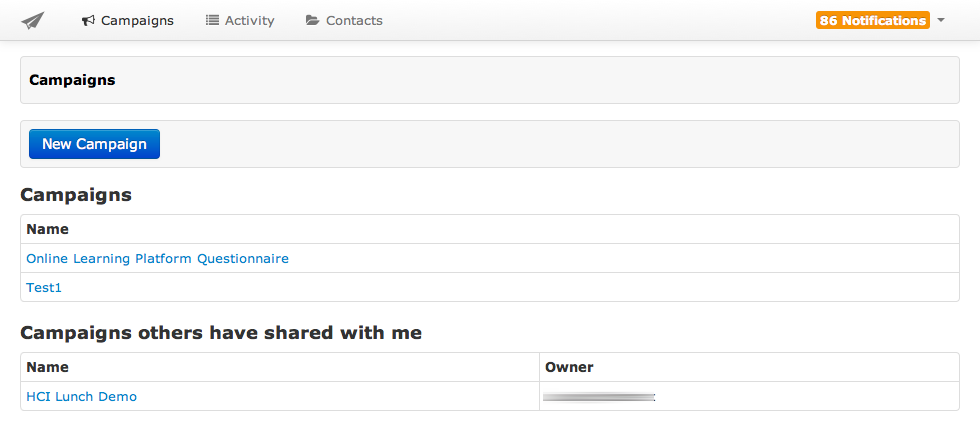
\includegraphics[width=1.00\textwidth]{imgs/CampaignsOverviewScreen.png}
	\caption[Myriad's Campaigns Overview Screen]{Myriad's Campaigns Overview Screen}
	\label{fig:CampaignsOverviewScreen}
\end{figure}

\subsection{Synchronization with Other Systems}
\label{subsec:5.2.2:SyncOtheSyst}

Myriad has the ability to get the recipients' information and their \ac{KVP}s from Google Spreadsheet\footnote{https://docs.google.com/spreadsheet/}. This is a convenient way in importing recipients' information into the system, since many people already keep their recipients' and related information in a spreadsheet environment as discussed in section \ref{subsec:5.1.3:ImpoExpoContInfo}. Therefore, Myriad offers a bi-directional syncing from and to a spreadsheet, as defined at beginning of the creation of a campaign. Besides this, Myriad also has an option to enter a recipient's first name, last name, and email address into the system directly.
\vspace{1cm}

The corresponding columns in a Google Spreadsheet start with "first name", "last name", and "email address" as shown in figure \ref{fig:GoogleSpreadsheet}. The rest of the columns will be filled out as a \ac{KVP}, and imported into the system as well.

\begin{figure}[htbp]
	\centering
	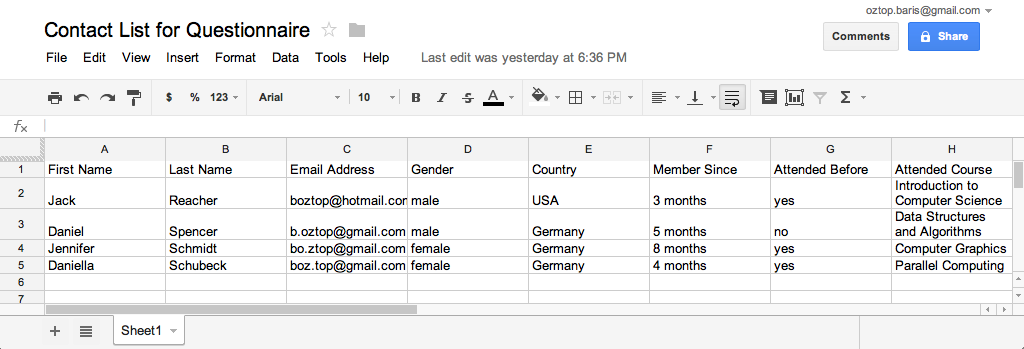
\includegraphics[width=1.00\textwidth]{imgs/GoogleSpreadsheet.png}
	\caption[A Google Spreadsheet to Import Recipients' Information into Myriad]{A Google Spreadsheet to Import Recipients' Information into Myriad}
	\label{fig:GoogleSpreadsheet}
\end{figure}

As mentioned in section \ref{subsec:5.1.4:InteEmaiClie}, importing existing email conversations as a campaign message into the system is an important feature. Researchers might have initiated conversations using their regular email client, and if later on they decide to make them more manageable, they can import them to Myriad. Myriad takes advantage of Gmail's labeling feature, which is equivalent to the \ac{IMAP} protocol's folders for the same purpose \citep{GoogleInc.2013}. Myriad creates a Gmail label in the user's account, and the only thing a user needs to do is the enable the label syncing feature at the campaign creation screen. Next, there will be a label similar to the campaign's name, and grouped under the root label, "myriad" in the Gmail's inbox (see figure \ref{fig:GmailLabels}). Hence, researchers will able to import email messages not considered a part of a campaign for some reason, into Myriad.

\begin{figure}[htbp]
	\centering
	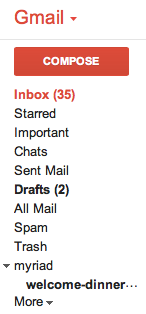
\includegraphics[scale=0.60]{imgs/GmailLabels.png}
	\caption[Gmail's Labels and Myriad's Campaigns Under the Myriad Label]{Gmail's Labels and Myriad's Campaigns Under the Myriad Label}
	\label{fig:GmailLabels}
\end{figure}

\subsection{Creating an Email Campaign}
\label{subsec:5.2.3:CreaEmaiCamp}

The campaign creation screen (see figure \ref{fig:CreateCampaign}) has input fields for a campaign name and Google Spreadsheet's \ac{URL} to synchronize with. Other two checkboxes for the spreadsheet are used to manage the frequency of synchronization and disabling the cascading warning messages in case of an erroneous data in the spreadsheet such as an empty email address field for a contact. The option for importing emails from Gmail's inbox is also in this screen, labeled as "synching section".

\begin{figure}[htbp]
	\centering
	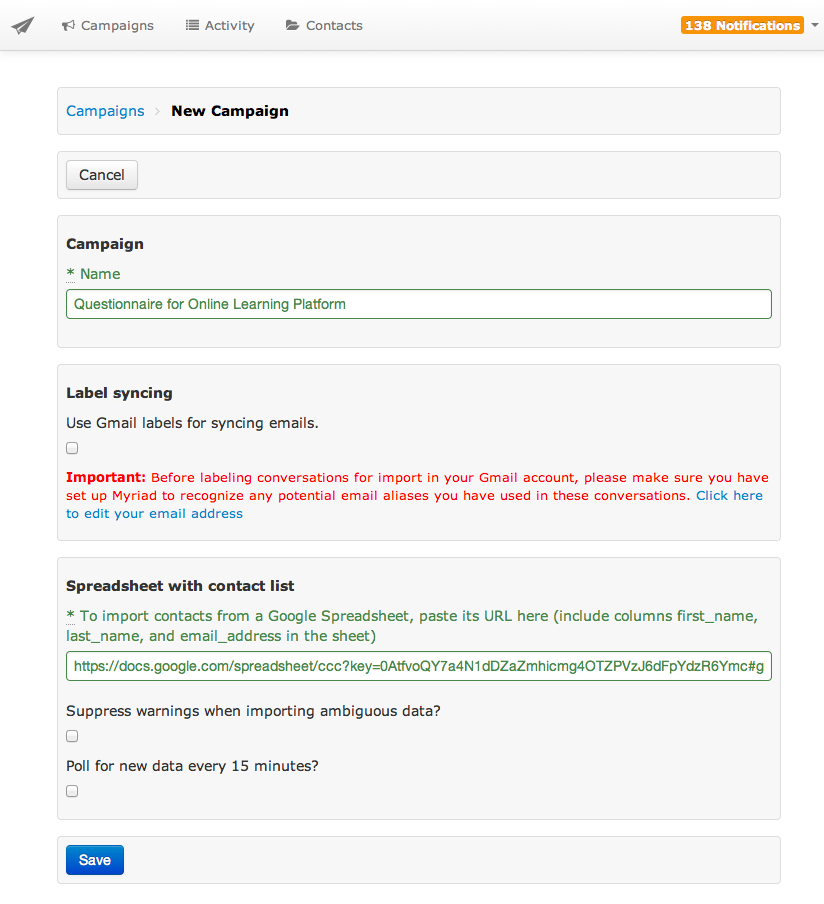
\includegraphics[width=1.00\textwidth]{imgs/CreateCampaign.png}
	\caption[Creating a Campaing in Myriad]{Creating a Campaing in Myriad}
	\label{fig:CreateCampaign}
\end{figure}

After the campaign is created, all the contacts and their \ac{KVP}s will be imported as long as the user provided a Google Spreadsheet \ac{URL} like in figure \ref{fig:ContactListInCampaign}.

\begin{figure}[htbp]
	\centering
	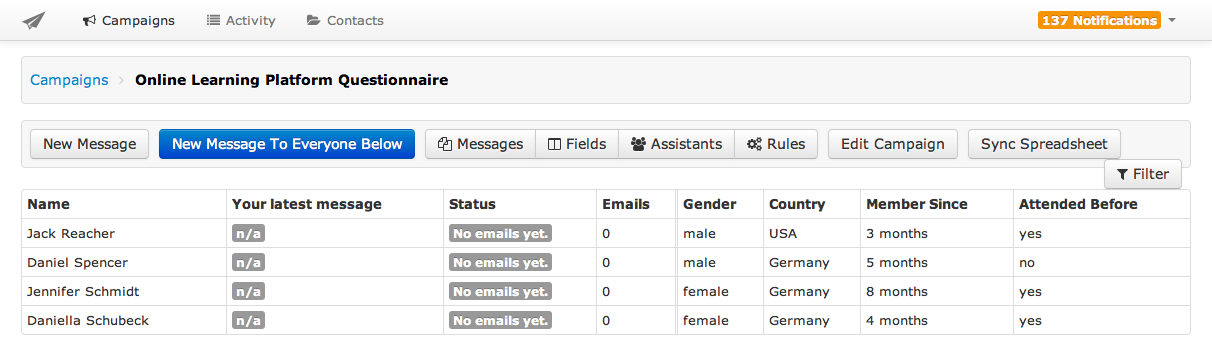
\includegraphics[width=1.00\textwidth]{imgs/ContactListInCampaign.png}
	\caption[Contacts and Their \ac{KVP}s After Synchronization in Myriad]{Contacts and Their \ac{KVP}s After Synchronization in Myriad}
	\label{fig:ContactListInCampaign}
\end{figure}

\clearpage

\subsection{Composing an Email Message}
\label{subsec:5.2.4:CompEmaiMess}

Users can send emails to all of the contacts they entered or imported into the system, or select a subset of them by using the filtering function as shown in figure \ref{fig:ContactFilters}. Provided filtering options are according to the values of \ac{KVP}s, the conversation statuses such as unread, replied, or unreplied, or the message's template names.
\vspace{1cm}

\begin{figure}[htbp]
	\centering
	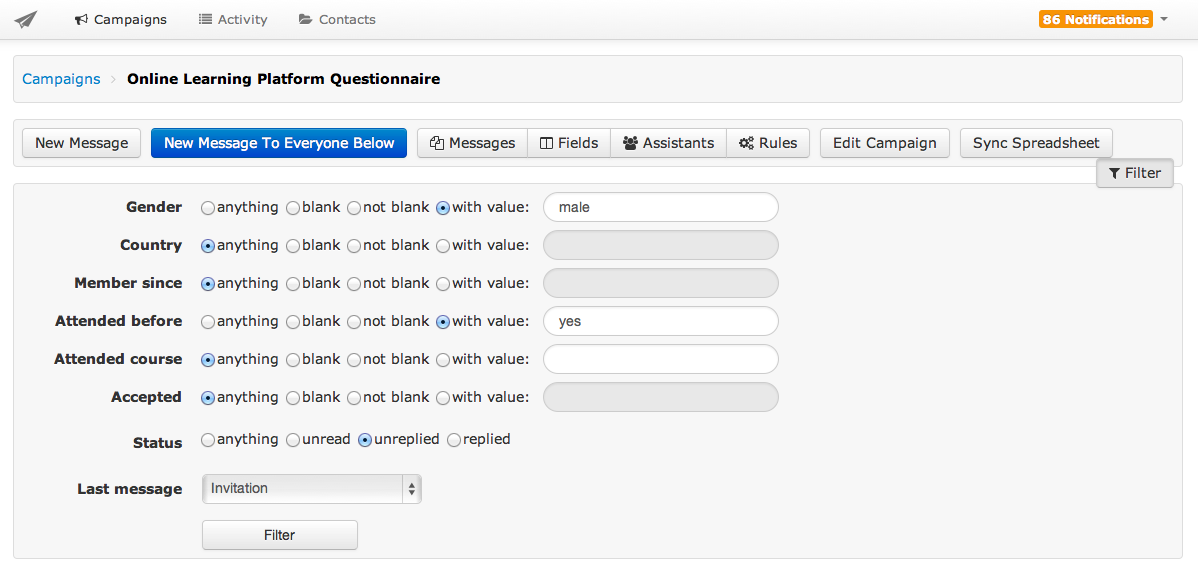
\includegraphics[width=1.00\textwidth]{imgs/ContactFilters.png}
	\caption[Filtering the Contact List in Myriad]{Filtering the Contact List in Myriad}
	\label{fig:ContactFilters}
\end{figure}

By pressing the corresponding button, users can now readily compose emails for their filtered recipients at the compose screen. The compose email pane (see figure \ref{fig:ComposeEmail}) contains a section that lists previously sent emails available for reuse. This is the same template concept that was introduced for the prototype in section \ref{subsec:4.2.2:ProtSyst}. It also shows the visualization of the state and flow of the communication by using a tree structure, as well as the number of messages sent by using the corresponding template. A more long term campaign's visualization tree can be found in appendix \ref{app:VisuCommStat}. The system also suggests an email template while composing a reply by considering the nodes at the same tree structure.
\vspace{1cm}

\begin{figure}[htbp]
	\centering
	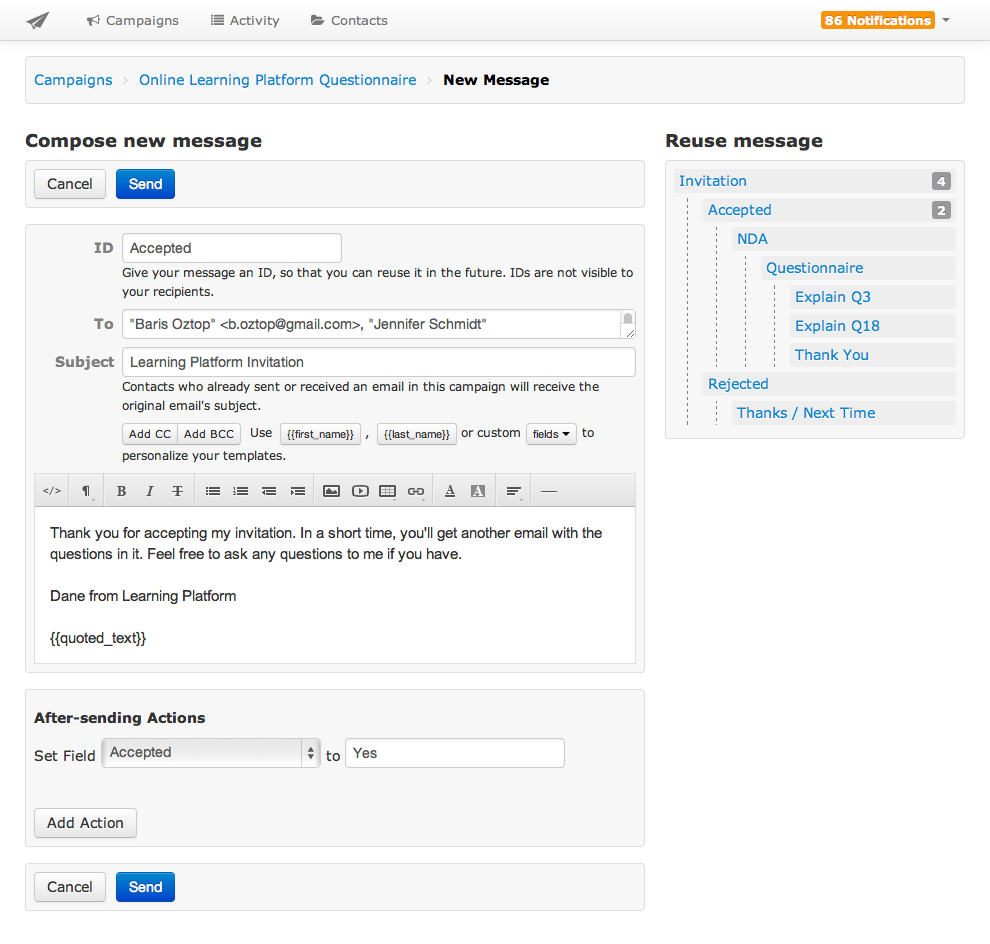
\includegraphics[width=1.00\textwidth]{imgs/ComposeEmail.png}
	\caption[Compose an Email in Myriad by Reusing Earlier Messages]{Compose an Email in Myriad by Reusing Earlier Messages}
	\label{fig:ComposeEmail}
\end{figure}

The compose pane allows users to add dynamic variables in the content of messages to personalize them according to the recipients. These variables are not just limited to the first name and last name, as they can also be of any keys from the assigned \ac{KVP}s in the campaign.
\vspace{1cm}

Each campaign has a link to the other campaigns, as long as the recipient is involved in both campaigns, as featured in the next section. A researcher can access conversations and \ac{KVP}s from other campaigns by switching to the campaign via the provided link. Providing an option to see the earlier campaigns a recipient got involved in gives broader knowledge about a recipient that may help researchers in personalizing the content of the emails more easily and properly. For example, if we have extracted information regarding which sports did the recipients got involved with in an earlier campaign. We can use the same information in making a friendlier and to frankly start a new campaign by mentioning details about the latest events of those sports areas in the country. Such a technique also supports the social exchange theory and the diffusion of responsibility theory as discussed in section \ref{sec:2.3:PersEmai}. There is also an option to hide the \ac{KVP}s in a campaign if they are not related at all or have become obsolete during the flow of a campaign to avoid cluttering the application's view.
\vspace{1cm}

In figure \ref{fig:ComposeEmail}, at the pane of "after-sending actions", users are able to set the values of the keys right after an email is sent. Therefore, a user does not need to browse to another screen in order to change or set \ac{KVP}s whose values depends on the email that was recently sent.
\vspace{1cm}

At the beginning of this section it was mentioned that a user can filter the recipients list, and then send an email to a subset, according to the filter's criteria. Myriad saves those filtered criteria under the "Rules" menu as shown in figure \ref{fig:AutomatedRules} after the user sent the email. Therefore, the next time the system receives new emails with the same conditions as before, user will see them under the rules menu, and the earlier sent email messages can be sent to those new matching recipients automatically, if user opt to enable the automated response feature or a user can simply press the send button manually in the same screen. For example, in figure \ref{fig:AutomatedRules}, there are three recipients whose "attending" key were set to "yes", and since the system already recognized that we have already sent an email to those attending, new matches for the same condition applies. In this case, the user can simply press the send button, or automate the process by enabling the provided option.

\begin{figure}[htbp]
	\centering
	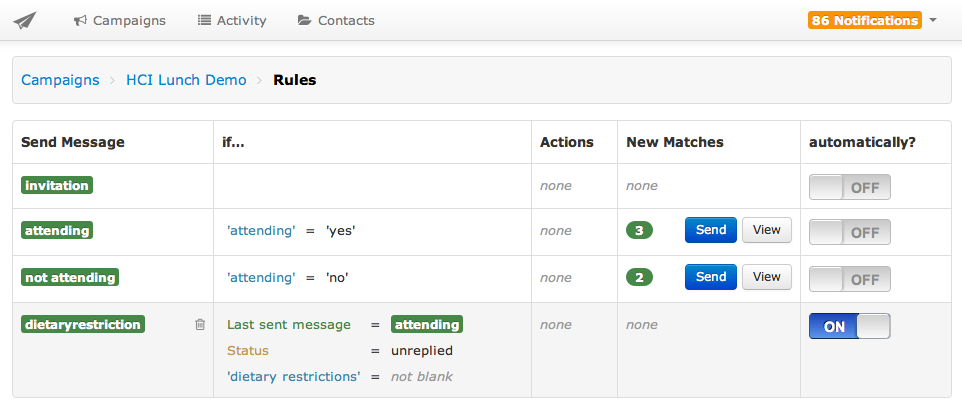
\includegraphics[width=1.00\textwidth]{imgs/AutomatedRules.png}
	\caption[Rules to Automate the Sending Process of the Emails in Myriad]{Rules to Automate the Sending Process of the Emails in Myriad}
	\label{fig:AutomatedRules}
\end{figure}

\subsection{Extracting Information from Email Messages}
\label{subsec:5.2.5:ExtrInfoEmaiMess}

Myriad's reading pane (see figure \ref{fig:MyriadReadingPane}) offers a threaded view wherein all of the messages between a specific recipient and a researcher are visually grouped together. The advantage of a threaded view is that it allows a researcher to get a quick overview of the whole state of a conversation, therefore a researcher can write a customized message more easily by focusing on the specific personality of the individual being responded to, considering earlier conversations with him or her at a single glance.
\vspace{1cm}

Each of the researcher's message is annotated with the name of the message template that was used with, making the latest state of the communication easily recognizable without having to look for its content. In figure \ref{fig:MyriadReadingPane}, emails sent by the user have green labels with indicators of the name of the template used, such as "Accepted" and "Invitation".
\vspace{1cm}

While reading a recipient's answer, the extracted information can be recorded as \ac{KVP}s at the right-hand side of the reading pane (see figure \ref{fig:MyriadReadingPane}). Earlier recorded keys' values can also be updated at the same pane. Having \ac{KVP}s along with the conversation thread gives the researcher necessary information about the person being replied to. Under the \ac{KVP}s pane, the researcher can also see if the recipient is involved with another campaign, and a link to the involved campaigns are provided with the number of emails exchanged, next to it. This is a helpful feature in reminding researchers about the existence of previous interactions with the recipient, and if necessary, the researcher can switch to other campaigns to get an overview of extracted information as \ac{KVP}s.
\vspace{1cm}

\begin{figure}[htbp]
	\centering
	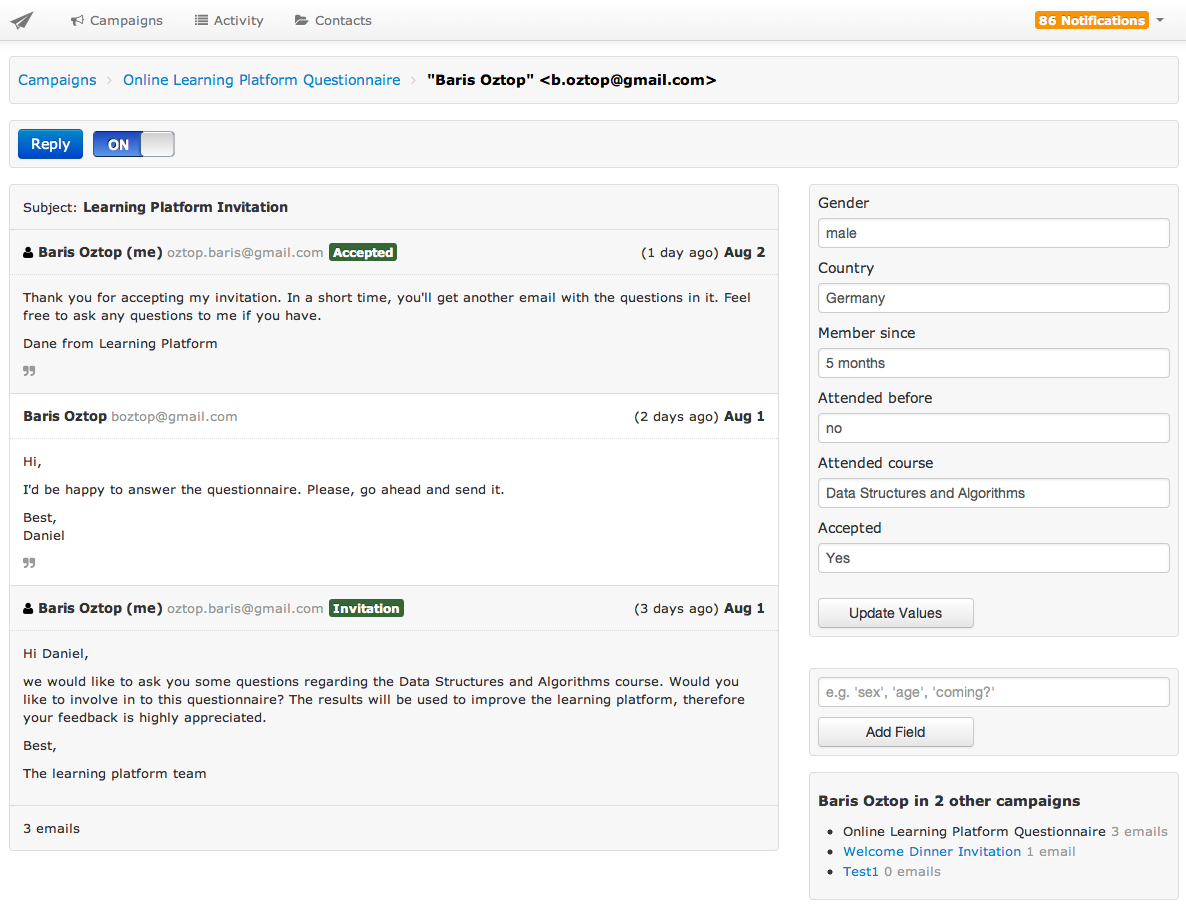
\includegraphics[width=1.00\textwidth]{imgs/MyriadReadingPane.png}
	\caption[The Reading Pane and the Extracted \ac{KVP}s in Myriad]{The Reading Pane and the Extracted \ac{KVP}s in Myriad}
	\label{fig:MyriadReadingPane}
\end{figure}

\subsection{Enabling Assistants}
\label{subsec:5.2.6:EnabAssi}

A researcher can add other researchers as assistants into a campaign by adding their Google account associated email addresses into Myriad, as shown in figure \ref{fig:AddAssistants}. The task of the assistant can range from extracting information from emails, writing answers to the recipients, to proofreading a researcher's emails before sending them, and many other tasks that can be generated according to the type of help a researcher needs.

\clearpage

\begin{figure}[htbp]
	\centering
	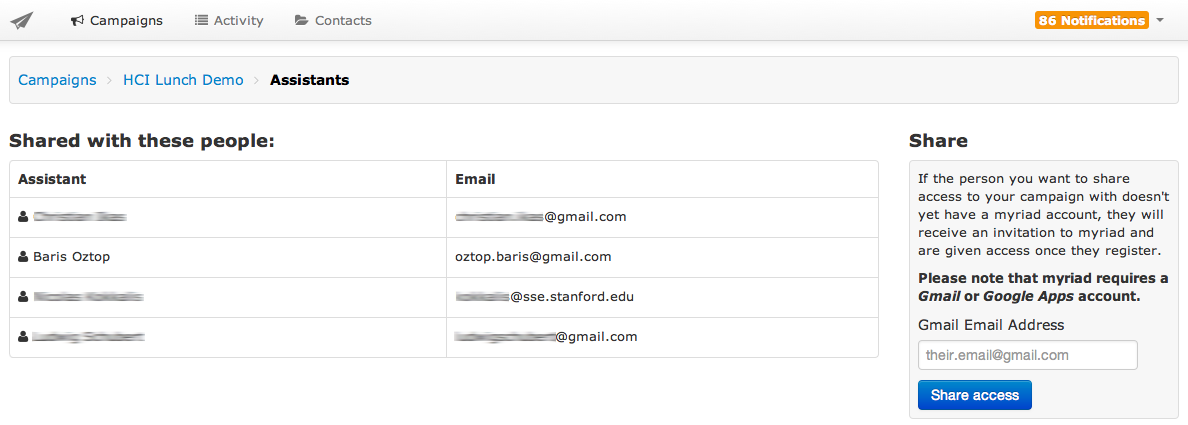
\includegraphics[width=1.00\textwidth]{imgs/AddAssistants.png}
	\caption[Rules to Automate the Sending Process of the Emails in Myriad]{Rules to Automate the Sending Process of the Emails in Myriad}
	\label{fig:AddAssistants}
\end{figure}

After an assistant is assigned to a campaign, he or she will get a notification email including the link to the campaign. Again, there will be a notification email for each email sent by a respondent to the assistants' email address to let them know that they need to act on the situation.
\vspace{1cm}

Myriad provides status labels for each received or sent email, giving a hint on the next awaiting action similar to what is shown in figure \ref{fig:EmailStatuses}. These status labels give hints about the next action to be taken according to the state of the conversation, such as if the user needs to read or to send a reply to a message, or the conversation awaits for an answer from the recipient's side to continue to the communication. There are also status labels related with Myriad's internal state regarding to an email message, such as if Myriad was able to send the messages successfully, or if there was a failure encountered while sending them. The same view also provides a column showing the name of the last message's template used to sent by the user. With this, the researchers and the assistants will easily realize what should be done next, and see the status of the communication for each recipient. 

\clearpage

\begin{figure}[htbp]
	\centering
	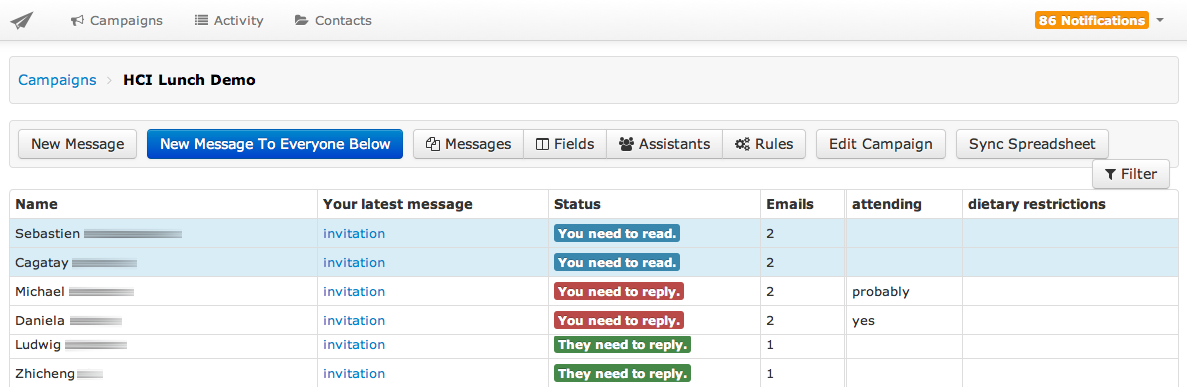
\includegraphics[width=1.00\textwidth]{imgs/EmailStatuses.png}
	\caption[Status Labels for Each Email in Myriad]{Status Labels for Each Email in Myriad}
	\label{fig:EmailStatuses}
\end{figure}

\section{Architecture}
\label{sec:5.3:FinaArch}

Similar to the prototype, Myriad was also developed using a framework stack of \ac{RoR}, jQuery, Bootstrap, and OAuth\footnote{OAuth is leveraged by using OmniAuth library (https://github.com/intridea/omniauth), and its Google authentication strategy is implementation by OmniAuth Google OAuth2. Details can be found at https://github.com/zquestz/omniauth-google-oauth2} protocol was used for the authentication with Gmail. The initial project structure was generated by a gem named Rails Apps Composer\footnote{https://github.com/RailsApps/rails\_apps\_composer}, consisting a collection of Rails application templates to start a project. Thanks to the other gems utilized for the project development and completing it on time in a robust way. The following section will discuss the implementation details of Myriad, how it makes mass email communication easier.

\subsection{Keeping Track of Recipients}
\label{subsec:5.3.1:ReciCont}

As mentioned in section \ref{sec:4.2:Prot}, the prototype was not able to keep the basic contact information of the recipients, only the messages of them. Therefore, extracted information such as \ac{KVP}s are only limited to email messages related to the recipients. The downside of this approach is its inability in obtaining all the \ac{KVP}s of the recipients all at one glance. Instead, we need to go through earlier emails of the recipients each time we need to create the same key, since the system was not aware of an existing \ac{KVP} created for a different email in the same campaign.
\vspace{1cm}

In Myriad's case, this issue was solved by keeping all the recipients' information in a separate data model named "contact" as shown in figure \ref{fig:UML_Draw_Final}. With this, we were able to keep track of the recipients among different campaigns through different conversations involving them, which is another set of a data model in the Myriad system, as each campaign involves many conversations with the recipient involved with them.
\vspace{1cm}

Myriad keeps all of the basic profile information of the recipients, including their first names, last names, and email addresses. These information can be imported into Myriad either by spreadsheet synchronization, by adding them into "To" filed when a user composes an email, or by importing from Gmail's inbox via the label synchronization. The recipients' email addresses are unique identifiers for Myriad in order to compare already existing recipient information with the synchronized ones. 

\begin{figure}[htbp]
	\centering
	\begin{pdfpic}
	    %LaTeX with PSTricks extensions
%%Creator: inkscape 0.48.2
%%Please note this file requires PSTricks extensions
\psset{xunit=.5pt,yunit=.5pt,runit=.5pt}
\begin{pspicture}(1183.75,1047.5)
{
\newrgbcolor{curcolor}{1 1 1}
\pscustom[linestyle=none,fillstyle=solid,fillcolor=curcolor]
{
\newpath
\moveto(0,739.0341375)
\lineto(835.254,739.0341375)
\lineto(835.254,-0.0818625)
\lineto(0,-0.0818625)
\closepath
}
}
{
\newrgbcolor{curcolor}{1 1 1}
\pscustom[linestyle=none,fillstyle=solid,fillcolor=curcolor]
{
\newpath
\moveto(0.882,540.35674026)
\lineto(267.77657592,540.35674026)
\lineto(267.77657592,515.66074026)
\lineto(0.882,515.66074026)
\closepath
\moveto(0.882,540.35674026)
}
}
{
\newrgbcolor{curcolor}{0 0 0}
\pscustom[linewidth=1.76400003,linecolor=curcolor]
{
\newpath
\moveto(0.882,540.35674026)
\lineto(267.77657592,540.35674026)
\lineto(267.77657592,515.66074026)
\lineto(0.882,515.66074026)
\closepath
\moveto(0.882,540.35674026)
}
}
{
\newrgbcolor{curcolor}{0 0 0}
\pscustom[linestyle=none,fillstyle=solid,fillcolor=curcolor]
{
\newpath
\moveto(113.0338125,524.16377813)
\curveto(112.54457768,523.91571563)(112.03467232,523.72622322)(111.50409375,523.59874688)
\curveto(110.98040625,523.46093438)(110.43260134,523.39202813)(109.864125,523.39202813)
\curveto(108.14491384,523.39202813)(106.78401518,523.86748169)(105.784875,524.82527813)
\curveto(104.78228884,525.78996563)(104.28271875,527.09229419)(104.28271875,528.73915313)
\curveto(104.28271875,530.38256697)(104.78228884,531.68144956)(105.784875,532.63924688)
\curveto(106.78401518,533.59359822)(108.14491384,534.07249688)(109.864125,534.07249688)
\curveto(110.43260134,534.07249688)(110.98040625,534.00703572)(111.50409375,533.87955938)
\curveto(112.03467232,533.74863706)(112.54457768,533.56259063)(113.0338125,533.31452813)
\lineto(113.0338125,531.17843438)
\curveto(112.54457768,531.51607456)(112.06223482,531.76413706)(111.58678125,531.92262188)
\curveto(111.10788259,532.07766072)(110.60142232,532.15690313)(110.07084375,532.15690313)
\curveto(109.12338259,532.15690313)(108.37919509,531.85371563)(107.83828125,531.24734063)
\curveto(107.29392232,530.64096563)(107.0251875,529.80375447)(107.0251875,528.73915313)
\curveto(107.0251875,527.67110669)(107.29392232,526.83734063)(107.83828125,526.23096563)
\curveto(108.37919509,525.62459063)(109.12338259,525.32140313)(110.07084375,525.32140313)
\curveto(110.60142232,525.32140313)(111.10788259,525.39719956)(111.58678125,525.55568438)
\curveto(112.06223482,525.71072322)(112.54457768,525.95878572)(113.0338125,526.29987188)
\closepath
\moveto(113.0338125,524.16377813)
}
}
{
\newrgbcolor{curcolor}{0 0 0}
\pscustom[linestyle=none,fillstyle=solid,fillcolor=curcolor]
{
\newpath
\moveto(118.79782031,529.74518438)
\curveto(118.24657031,529.74518438)(117.82624175,529.54535669)(117.54372656,529.15259063)
\curveto(117.2577654,528.75637947)(117.11650781,528.19134822)(117.11650781,527.45749688)
\curveto(117.11650781,526.71330938)(117.2577654,526.14138706)(117.54372656,525.74862188)
\curveto(117.82624175,525.36274688)(118.24657031,525.16980938)(118.79782031,525.16980938)
\curveto(119.32839888,525.16980938)(119.7383904,525.36274688)(120.02435156,525.74862188)
\curveto(120.30686675,526.14138706)(120.45157031,526.71330938)(120.45157031,527.45749688)
\curveto(120.45157031,528.19134822)(120.30686675,528.75637947)(120.02435156,529.15259063)
\curveto(119.7383904,529.54535669)(119.32839888,529.74518438)(118.79782031,529.74518438)
\closepath
\moveto(118.79782031,531.50918438)
\curveto(120.12082031,531.50918438)(121.15441406,531.15087188)(121.89860156,530.43424688)
\curveto(122.64967925,529.71762188)(123.02866406,528.72537188)(123.02866406,527.45749688)
\curveto(123.02866406,526.18962188)(122.64967925,525.19048169)(121.89860156,524.46696563)
\curveto(121.15441406,523.75034063)(120.12082031,523.39202813)(118.79782031,523.39202813)
\curveto(117.46448415,523.39202813)(116.42055425,523.75034063)(115.66947656,524.46696563)
\curveto(114.9149529,525.19048169)(114.53941406,526.18962188)(114.53941406,527.45749688)
\curveto(114.53941406,528.72537188)(114.9149529,529.71762188)(115.66947656,530.43424688)
\curveto(116.42055425,531.15087188)(117.46448415,531.50918438)(118.79782031,531.50918438)
\closepath
\moveto(118.79782031,531.50918438)
}
}
{
\newrgbcolor{curcolor}{0 0 0}
\pscustom[linestyle=none,fillstyle=solid,fillcolor=curcolor]
{
\newpath
\moveto(132.575625,528.29815313)
\lineto(132.575625,523.59874688)
\lineto(130.095,523.59874688)
\lineto(130.095,527.19565313)
\curveto(130.095,527.86404419)(130.08121875,528.32571563)(130.05365625,528.57377813)
\curveto(130.02609375,528.82873169)(129.97441384,529.01822322)(129.9020625,529.13880938)
\curveto(129.79870357,529.29384822)(129.66778125,529.41787947)(129.50240625,529.51090313)
\curveto(129.33703125,529.60048169)(129.14753884,529.64871563)(128.937375,529.64871563)
\curveto(128.42057857,529.64871563)(128.01747634,529.44544197)(127.724625,529.04234063)
\curveto(127.42832857,528.64612947)(127.283625,528.09832456)(127.283625,527.40237188)
\lineto(127.283625,523.59874688)
\lineto(124.81678125,523.59874688)
\lineto(124.81678125,531.31624688)
\lineto(127.283625,531.31624688)
\lineto(127.283625,530.18618438)
\curveto(127.65916384,530.63407456)(128.055375,530.96482456)(128.4688125,531.17843438)
\curveto(128.88914107,531.39893438)(129.35425759,531.50918438)(129.86071875,531.50918438)
\curveto(130.74960893,531.50918438)(131.42489107,531.23355938)(131.8865625,530.68230938)
\curveto(132.34478884,530.13794956)(132.575625,529.34552813)(132.575625,528.29815313)
\closepath
\moveto(132.575625,528.29815313)
}
}
{
\newrgbcolor{curcolor}{0 0 0}
\pscustom[linestyle=none,fillstyle=solid,fillcolor=curcolor]
{
\newpath
\moveto(137.56099219,533.50746563)
\lineto(137.56099219,531.31624688)
\lineto(140.09674219,531.31624688)
\lineto(140.09674219,529.55224688)
\lineto(137.56099219,529.55224688)
\lineto(137.56099219,526.28609063)
\curveto(137.56099219,525.92777813)(137.62989844,525.68316072)(137.76771094,525.55568438)
\curveto(137.9124145,525.42476206)(138.19837478,525.36274688)(138.62214844,525.36274688)
\lineto(139.89002344,525.36274688)
\lineto(139.89002344,523.59874688)
\lineto(137.76771094,523.59874688)
\curveto(136.79268728,523.59874688)(136.10362478,523.79857456)(135.70052344,524.20512188)
\curveto(135.293977,524.61855938)(135.09414844,525.31106697)(135.09414844,526.28609063)
\lineto(135.09414844,529.55224688)
\lineto(133.86761719,529.55224688)
\lineto(133.86761719,531.31624688)
\lineto(135.09414844,531.31624688)
\lineto(135.09414844,533.50746563)
\closepath
\moveto(137.56099219,533.50746563)
}
}
{
\newrgbcolor{curcolor}{0 0 0}
\pscustom[linestyle=none,fillstyle=solid,fillcolor=curcolor]
{
\newpath
\moveto(145.07177344,527.07162188)
\curveto(144.554977,527.07162188)(144.169102,526.98204419)(143.91414844,526.80977813)
\curveto(143.65574978,526.63406697)(143.52827344,526.37566919)(143.52827344,526.03802813)
\curveto(143.52827344,525.72450447)(143.62818728,525.47988706)(143.83146094,525.30762188)
\curveto(144.04162478,525.13191072)(144.334477,525.04577813)(144.71346094,525.04577813)
\curveto(145.17168728,525.04577813)(145.55756228,525.21115313)(145.87108594,525.54190313)
\curveto(146.19149978,525.87265313)(146.35342969,526.28953572)(146.35342969,526.79599688)
\lineto(146.35342969,527.07162188)
\closepath
\moveto(148.84783594,528.00874688)
\lineto(148.84783594,523.59874688)
\lineto(146.35342969,523.59874688)
\lineto(146.35342969,524.74259063)
\curveto(146.02267969,524.27402813)(145.65058594,523.92949688)(145.23714844,523.70899688)
\curveto(144.82371094,523.49883303)(144.32069487,523.39202813)(143.73499219,523.39202813)
\curveto(142.93567969,523.39202813)(142.28106987,523.62630938)(141.77805469,524.09487188)
\curveto(141.28192969,524.56343438)(141.03386719,525.16980938)(141.03386719,525.91399688)
\curveto(141.03386719,526.82355938)(141.34394487,527.48850447)(141.97099219,527.91227813)
\curveto(142.59459353,528.33260669)(143.57306228,528.54621563)(144.90639844,528.54621563)
\lineto(146.35342969,528.54621563)
\lineto(146.35342969,528.73915313)
\curveto(146.35342969,529.12502813)(146.19494487,529.40754419)(145.88486719,529.59359063)
\curveto(145.58167969,529.77619197)(145.10278103,529.86921563)(144.45161719,529.86921563)
\curveto(143.92792969,529.86921563)(143.43524978,529.81409063)(142.97702344,529.70384063)
\curveto(142.52568728,529.60048169)(142.1019145,529.44544197)(141.70914844,529.23527813)
\lineto(141.70914844,531.10952813)
\curveto(142.239727,531.23700447)(142.77374978,531.33347322)(143.30777344,531.39893438)
\curveto(143.838352,531.47128572)(144.37237478,531.50918438)(144.90639844,531.50918438)
\curveto(146.2914145,531.50918438)(147.29399978,531.23355938)(147.91071094,530.68230938)
\curveto(148.53431228,530.13105938)(148.84783594,529.23872322)(148.84783594,528.00874688)
\closepath
\moveto(148.84783594,528.00874688)
}
}
{
\newrgbcolor{curcolor}{0 0 0}
\pscustom[linestyle=none,fillstyle=solid,fillcolor=curcolor]
{
\newpath
\moveto(157.381875,531.08196563)
\lineto(157.381875,529.06990313)
\curveto(157.04078884,529.29729419)(156.69970357,529.46955938)(156.3620625,529.57980938)
\curveto(156.0313125,529.69005938)(155.67989107,529.74518438)(155.3146875,529.74518438)
\curveto(154.625625,529.74518438)(154.08815625,529.54191072)(153.70228125,529.13880938)
\curveto(153.32329643,528.73226206)(153.13725,528.17412188)(153.13725,527.45749688)
\curveto(153.13725,526.73053572)(153.32329643,526.16550447)(153.70228125,525.76240313)
\curveto(154.08815625,525.36619197)(154.625625,525.16980938)(155.3146875,525.16980938)
\curveto(155.7005625,525.16980938)(156.06576607,525.22493438)(156.4171875,525.33518438)
\curveto(156.76516384,525.45232456)(157.08557857,525.62459063)(157.381875,525.84509063)
\lineto(157.381875,523.83302813)
\curveto(156.996,523.68487964)(156.59978884,523.578075)(156.1966875,523.50227813)
\curveto(155.80047634,523.42992678)(155.40426607,523.39202813)(155.0115,523.39202813)
\curveto(153.61270357,523.39202813)(152.52053884,523.75034063)(151.7315625,524.46696563)
\curveto(150.94947634,525.18359063)(150.56015625,526.17928572)(150.56015625,527.45749688)
\curveto(150.56015625,528.72537188)(150.94947634,529.71762188)(151.7315625,530.43424688)
\curveto(152.52053884,531.15087188)(153.61270357,531.50918438)(155.0115,531.50918438)
\curveto(155.41460134,531.50918438)(155.8108125,531.47128572)(156.1966875,531.39893438)
\curveto(156.58945357,531.32313706)(156.98566384,531.21977813)(157.381875,531.08196563)
\closepath
\moveto(157.381875,531.08196563)
}
}
{
\newrgbcolor{curcolor}{0 0 0}
\pscustom[linestyle=none,fillstyle=solid,fillcolor=curcolor]
{
\newpath
\moveto(162.21220313,533.50746563)
\lineto(162.21220313,531.31624688)
\lineto(164.74795313,531.31624688)
\lineto(164.74795313,529.55224688)
\lineto(162.21220313,529.55224688)
\lineto(162.21220313,526.28609063)
\curveto(162.21220313,525.92777813)(162.28110937,525.68316072)(162.41892187,525.55568438)
\curveto(162.56362544,525.42476206)(162.84958572,525.36274688)(163.27335938,525.36274688)
\lineto(164.54123437,525.36274688)
\lineto(164.54123437,523.59874688)
\lineto(162.41892187,523.59874688)
\curveto(161.44389822,523.59874688)(160.75483572,523.79857456)(160.35173438,524.20512188)
\curveto(159.94518794,524.61855938)(159.74535937,525.31106697)(159.74535937,526.28609063)
\lineto(159.74535937,529.55224688)
\lineto(158.51882812,529.55224688)
\lineto(158.51882812,531.31624688)
\lineto(159.74535937,531.31624688)
\lineto(159.74535937,533.50746563)
\closepath
\moveto(162.21220313,533.50746563)
}
}
{
\newrgbcolor{curcolor}{1 1 1}
\pscustom[linestyle=none,fillstyle=solid,fillcolor=curcolor]
{
\newpath
\moveto(0.882,515.66074026)
\lineto(267.77657592,515.66074026)
\lineto(267.77657592,342.78874026)
\lineto(0.882,342.78874026)
\closepath
\moveto(0.882,515.66074026)
}
}
{
\newrgbcolor{curcolor}{0 0 0}
\pscustom[linewidth=1.76400003,linecolor=curcolor]
{
\newpath
\moveto(0.882,515.66074026)
\lineto(267.77657592,515.66074026)
\lineto(267.77657592,342.78874026)
\lineto(0.882,342.78874026)
\closepath
\moveto(0.882,515.66074026)
}
}
{
\newrgbcolor{curcolor}{0 0 0}
\pscustom[linestyle=none,fillstyle=solid,fillcolor=curcolor]
{
\newpath
\moveto(16.37557031,503.62971563)
\curveto(16.09994531,503.47123169)(15.81398415,503.35409063)(15.52113281,503.27140313)
\curveto(15.22483638,503.18871563)(14.92853906,503.14737188)(14.62535156,503.14737188)
\curveto(13.6503279,503.14737188)(12.88891406,503.43677812)(12.33766406,504.01559063)
\curveto(11.79330425,504.60129419)(11.52457031,505.41094197)(11.52457031,506.44109063)
\curveto(11.52457031,507.46779419)(11.79330425,508.27399688)(12.33766406,508.85280937)
\curveto(12.88891406,509.43851206)(13.6503279,509.73480937)(14.62535156,509.73480937)
\curveto(14.92853906,509.73480937)(15.2213904,509.69346563)(15.50735156,509.61077813)
\curveto(15.78986675,509.53498169)(16.07927388,509.41784062)(16.37557031,509.25246563)
\lineto(16.37557031,508.17752813)
\curveto(16.09994531,508.41525447)(15.82432031,508.59096563)(15.54869531,508.70121563)
\curveto(15.27996138,508.81146563)(14.9733279,508.86659063)(14.62535156,508.86659063)
\curveto(13.9810779,508.86659063)(13.4849529,508.65298169)(13.13697656,508.23265313)
\curveto(12.78555425,507.81921563)(12.61328906,507.21973169)(12.61328906,506.44109063)
\curveto(12.61328906,505.66934063)(12.78555425,505.06985669)(13.13697656,504.64952813)
\curveto(13.4849529,504.23609063)(13.9810779,504.02937188)(14.62535156,504.02937188)
\curveto(14.98366406,504.02937188)(15.3040779,504.08449688)(15.59003906,504.19474688)
\curveto(15.87255425,504.30499688)(16.13439888,504.47381697)(16.37557031,504.70465312)
\closepath
\moveto(16.37557031,503.62971563)
}
}
{
\newrgbcolor{curcolor}{0 0 0}
\pscustom[linestyle=none,fillstyle=solid,fillcolor=curcolor]
{
\newpath
\moveto(21.27135938,506.46865313)
\lineto(20.92682813,506.46865313)
\curveto(20.32734331,506.46865313)(19.87945313,506.36184822)(19.57626563,506.15168438)
\curveto(19.27307813,505.93807456)(19.12148438,505.62110669)(19.12148438,505.20077812)
\curveto(19.12148438,504.82179419)(19.23173438,504.52894197)(19.45223437,504.31877812)
\curveto(19.67962544,504.11550447)(19.99659331,504.01559063)(20.40314063,504.01559063)
\curveto(20.97161697,504.01559063)(21.41606294,504.21197322)(21.73992188,504.60818438)
\curveto(22.07067188,505.00094956)(22.23604687,505.54530937)(22.23604687,506.23437188)
\lineto(22.23604687,506.46865313)
\closepath
\moveto(23.26964063,506.89587188)
\lineto(23.26964063,503.31274688)
\lineto(22.23604687,503.31274688)
\lineto(22.23604687,504.23609063)
\curveto(22.01554688,503.86744197)(21.73303081,503.59181697)(21.39539063,503.40921563)
\curveto(21.06464063,503.23695)(20.65809331,503.14737188)(20.18264063,503.14737188)
\curveto(19.54870313,503.14737188)(19.03879688,503.32652813)(18.65292188,503.68484062)
\curveto(18.27393794,504.05004419)(18.08789062,504.53238706)(18.08789062,505.13187188)
\curveto(18.08789062,505.82782456)(18.32217188,506.35840312)(18.79073437,506.71671563)
\curveto(19.25929688,507.08191919)(19.94835938,507.26796562)(20.85792188,507.26796562)
\lineto(22.23604687,507.26796562)
\lineto(22.23604687,507.43334063)
\curveto(22.23604687,507.92946563)(22.10512544,508.29122322)(21.85017188,508.52205938)
\curveto(21.60210938,508.74944956)(21.20589822,508.86659063)(20.66498438,508.86659063)
\curveto(20.30667187,508.86659063)(19.94835938,508.81491072)(19.59004688,508.71499687)
\curveto(19.23173438,508.61163706)(18.88031294,508.46693437)(18.54267187,508.27399688)
\lineto(18.54267187,509.29380938)
\curveto(18.92854688,509.43851206)(19.29375044,509.54876206)(19.64517188,509.62455937)
\curveto(19.99314822,509.69691072)(20.33423438,509.73480937)(20.66498438,509.73480937)
\curveto(21.17833572,509.73480937)(21.61933572,509.65556697)(21.98798437,509.50052813)
\curveto(22.35318794,509.35237947)(22.65292947,509.12154419)(22.88376563,508.81146563)
\curveto(23.02157813,508.62541919)(23.11804688,508.39802812)(23.17317188,508.12240313)
\curveto(23.23518794,507.84677813)(23.26964063,507.43678572)(23.26964063,506.89587188)
\closepath
\moveto(23.26964063,506.89587188)
}
}
{
\newrgbcolor{curcolor}{0 0 0}
\pscustom[linestyle=none,fillstyle=solid,fillcolor=curcolor]
{
\newpath
\moveto(28.04139844,508.94927813)
\curveto(28.1585395,509.21456697)(28.31702344,509.41094956)(28.50996094,509.54187188)
\curveto(28.7097895,509.66934822)(28.95096094,509.73480937)(29.22658594,509.73480937)
\curveto(29.729602,509.73480937)(30.08446853,509.53498169)(30.28774219,509.14221563)
\curveto(30.49790603,508.75634063)(30.60471094,508.02593438)(30.60471094,506.95099688)
\lineto(30.60471094,503.31274688)
\lineto(29.66758594,503.31274688)
\lineto(29.66758594,506.89587188)
\curveto(29.66758594,507.78476206)(29.61590603,508.33601206)(29.51599219,508.54962188)
\curveto(29.41263237,508.75978572)(29.233477,508.86659063)(28.97852344,508.86659063)
\curveto(28.67533594,508.86659063)(28.46861719,508.74944956)(28.35836719,508.52205938)
\curveto(28.24811719,508.29122322)(28.19299219,507.75030938)(28.19299219,506.89587188)
\lineto(28.19299219,503.31274688)
\lineto(27.25586719,503.31274688)
\lineto(27.25586719,506.89587188)
\curveto(27.25586719,507.79509822)(27.20074219,508.34634822)(27.09049219,508.54962188)
\curveto(26.98713237,508.75978572)(26.80108594,508.86659063)(26.52546094,508.86659063)
\curveto(26.24983594,508.86659063)(26.05689844,508.74944956)(25.94664844,508.52205938)
\curveto(25.8432895,508.29122322)(25.79505469,507.75030938)(25.79505469,506.89587188)
\lineto(25.79505469,503.31274688)
\lineto(24.85792969,503.31274688)
\lineto(24.85792969,509.58321563)
\lineto(25.79505469,509.58321563)
\lineto(25.79505469,509.04574688)
\curveto(25.92253103,509.26624688)(26.07756987,509.43506697)(26.26361719,509.55565312)
\curveto(26.44621853,509.67279419)(26.65293728,509.73480937)(26.88377344,509.73480937)
\curveto(27.1662895,509.73480937)(27.40056987,509.66934822)(27.58661719,509.54187188)
\curveto(27.77955469,509.41094956)(27.93114844,509.21456697)(28.04139844,508.94927813)
\closepath
\moveto(28.04139844,508.94927813)
}
}
{
\newrgbcolor{curcolor}{0 0 0}
\pscustom[linestyle=none,fillstyle=solid,fillcolor=curcolor]
{
\newpath
\moveto(33.25415625,504.09827813)
\lineto(33.25415625,500.92859063)
\lineto(32.2205625,500.92859063)
\lineto(32.2205625,509.58321563)
\lineto(33.25415625,509.58321563)
\lineto(33.25415625,508.78390312)
\curveto(33.42642143,509.09398169)(33.65725759,509.32826206)(33.94321875,509.48674687)
\curveto(34.22573393,509.65212188)(34.55648393,509.73480937)(34.93546875,509.73480937)
\curveto(35.68654643,509.73480937)(36.27914107,509.43851206)(36.71325,508.85280937)
\curveto(37.14391384,508.26366072)(37.36096875,507.45056697)(37.36096875,506.41352813)
\curveto(37.36096875,505.40060669)(37.14391384,504.60129419)(36.71325,504.01559063)
\curveto(36.27914107,503.43677812)(35.68654643,503.14737188)(34.93546875,503.14737188)
\curveto(34.54959375,503.14737188)(34.21195357,503.23005937)(33.9294375,503.39543438)
\curveto(33.64347634,503.56080938)(33.41953125,503.79509063)(33.25415625,504.09827813)
\closepath
\moveto(36.28603125,506.44109063)
\curveto(36.28603125,507.24040313)(36.15510893,507.83988706)(35.90015625,508.24643438)
\curveto(35.65209375,508.65987188)(35.28,508.86659063)(34.783875,508.86659063)
\curveto(34.27741384,508.86659063)(33.89498393,508.65987188)(33.64003125,508.24643438)
\curveto(33.38163259,507.83988706)(33.25415625,507.24040313)(33.25415625,506.44109063)
\curveto(33.25415625,505.64866919)(33.38163259,505.04918438)(33.64003125,504.63574687)
\curveto(33.89498393,504.22919956)(34.27741384,504.02937188)(34.783875,504.02937188)
\curveto(35.28,504.02937188)(35.65209375,504.22919956)(35.90015625,504.63574687)
\curveto(36.15510893,505.03884822)(36.28603125,505.64177813)(36.28603125,506.44109063)
\closepath
\moveto(36.28603125,506.44109063)
}
}
{
\newrgbcolor{curcolor}{0 0 0}
\pscustom[linestyle=none,fillstyle=solid,fillcolor=curcolor]
{
\newpath
\moveto(41.99491406,506.46865313)
\lineto(41.65038281,506.46865313)
\curveto(41.050898,506.46865313)(40.60300781,506.36184822)(40.29982031,506.15168438)
\curveto(39.99663281,505.93807456)(39.84503906,505.62110669)(39.84503906,505.20077812)
\curveto(39.84503906,504.82179419)(39.95528906,504.52894197)(40.17578906,504.31877812)
\curveto(40.40318013,504.11550447)(40.720148,504.01559063)(41.12669531,504.01559063)
\curveto(41.69517165,504.01559063)(42.13961763,504.21197322)(42.46347656,504.60818438)
\curveto(42.79422656,505.00094956)(42.95960156,505.54530937)(42.95960156,506.23437188)
\lineto(42.95960156,506.46865313)
\closepath
\moveto(43.99319531,506.89587188)
\lineto(43.99319531,503.31274688)
\lineto(42.95960156,503.31274688)
\lineto(42.95960156,504.23609063)
\curveto(42.73910156,503.86744197)(42.4565855,503.59181697)(42.11894531,503.40921563)
\curveto(41.78819531,503.23695)(41.381648,503.14737188)(40.90619531,503.14737188)
\curveto(40.27225781,503.14737188)(39.76235156,503.32652813)(39.37647656,503.68484062)
\curveto(38.99749263,504.05004419)(38.81144531,504.53238706)(38.81144531,505.13187188)
\curveto(38.81144531,505.82782456)(39.04572656,506.35840312)(39.51428906,506.71671563)
\curveto(39.98285156,507.08191919)(40.67191406,507.26796562)(41.58147656,507.26796562)
\lineto(42.95960156,507.26796562)
\lineto(42.95960156,507.43334063)
\curveto(42.95960156,507.92946563)(42.82868013,508.29122322)(42.57372656,508.52205938)
\curveto(42.32566406,508.74944956)(41.9294529,508.86659063)(41.38853906,508.86659063)
\curveto(41.03022656,508.86659063)(40.67191406,508.81491072)(40.31360156,508.71499687)
\curveto(39.95528906,508.61163706)(39.60386763,508.46693437)(39.26622656,508.27399688)
\lineto(39.26622656,509.29380938)
\curveto(39.65210156,509.43851206)(40.01730513,509.54876206)(40.36872656,509.62455937)
\curveto(40.7167029,509.69691072)(41.05778906,509.73480937)(41.38853906,509.73480937)
\curveto(41.9018904,509.73480937)(42.3428904,509.65556697)(42.71153906,509.50052813)
\curveto(43.07674263,509.35237947)(43.37648415,509.12154419)(43.60732031,508.81146563)
\curveto(43.74513281,508.62541919)(43.84160156,508.39802812)(43.89672656,508.12240313)
\curveto(43.95874263,507.84677813)(43.99319531,507.43678572)(43.99319531,506.89587188)
\closepath
\moveto(43.99319531,506.89587188)
}
}
{
\newrgbcolor{curcolor}{0 0 0}
\pscustom[linestyle=none,fillstyle=solid,fillcolor=curcolor]
{
\newpath
\moveto(46.40835938,509.58321563)
\lineto(49.04057813,509.58321563)
\lineto(49.04057813,504.11205938)
\lineto(51.09398438,504.11205938)
\lineto(51.09398438,503.31274688)
\lineto(45.96735938,503.31274688)
\lineto(45.96735938,504.11205938)
\lineto(48.02076563,504.11205938)
\lineto(48.02076563,508.78390312)
\lineto(46.40835938,508.78390312)
\closepath
\moveto(48.02076563,512.02249688)
\lineto(49.04057813,512.02249688)
\lineto(49.04057813,510.71327812)
\lineto(48.02076563,510.71327812)
\closepath
\moveto(48.02076563,512.02249688)
}
}
{
\newrgbcolor{curcolor}{0 0 0}
\pscustom[linestyle=none,fillstyle=solid,fillcolor=curcolor]
{
\newpath
\moveto(56.69261719,506.49621562)
\curveto(56.69261719,507.26796562)(56.56169575,507.85366919)(56.30674219,508.26021563)
\curveto(56.05867969,508.66331697)(55.69003103,508.86659063)(55.20424219,508.86659063)
\curveto(54.69778103,508.86659063)(54.31190603,508.66331697)(54.04661719,508.26021563)
\curveto(53.78821853,507.85366919)(53.66074219,507.26796562)(53.66074219,506.49621562)
\curveto(53.66074219,505.72446562)(53.79166362,505.13531697)(54.06039844,504.73221563)
\curveto(54.32568728,504.32566919)(54.71156228,504.12584063)(55.21802344,504.12584063)
\curveto(55.69347612,504.12584063)(56.05867969,504.32566919)(56.30674219,504.73221563)
\curveto(56.56169575,505.13531697)(56.69261719,505.72446562)(56.69261719,506.49621562)
\closepath
\moveto(57.71242969,503.71240313)
\curveto(57.71242969,502.77527812)(57.49192969,502.06554419)(57.05092969,501.57630937)
\curveto(56.60992969,501.09052053)(55.95532075,500.84590313)(55.09399219,500.84590313)
\curveto(54.80803103,500.84590313)(54.50828862,500.87346562)(54.19821094,500.92859063)
\curveto(53.88468728,500.98371563)(53.57805469,501.06295803)(53.27486719,501.16287188)
\lineto(53.27486719,502.18268438)
\curveto(53.64007075,502.01041919)(53.97082075,501.87949688)(54.26711719,501.79680938)
\curveto(54.57030469,501.71412187)(54.84592969,501.67277813)(55.09399219,501.67277813)
\curveto(55.64524219,501.67277813)(56.04834353,501.82437187)(56.30674219,502.12755938)
\curveto(56.56169575,502.43074688)(56.69261719,502.90964553)(56.69261719,503.56080938)
\lineto(56.69261719,504.30499688)
\curveto(56.52724219,503.95357456)(56.29985112,503.69173169)(56.01733594,503.51946563)
\curveto(55.73137478,503.35409063)(55.38684353,503.27140313)(54.98374219,503.27140313)
\curveto(54.24644575,503.27140313)(53.66074219,503.56080938)(53.21974219,504.13962187)
\curveto(52.78563325,504.72532456)(52.57202344,505.51085669)(52.57202344,506.49621562)
\curveto(52.57202344,507.47812947)(52.78563325,508.26366072)(53.21974219,508.85280937)
\curveto(53.66074219,509.43851206)(54.24644575,509.73480937)(54.98374219,509.73480937)
\curveto(55.38684353,509.73480937)(55.72792969,509.65212188)(56.00355469,509.48674687)
\curveto(56.27917969,509.32826206)(56.50657075,509.08019956)(56.69261719,508.74255938)
\lineto(56.69261719,509.55565312)
\lineto(57.71242969,509.55565312)
\closepath
\moveto(57.71242969,503.71240313)
}
}
{
\newrgbcolor{curcolor}{0 0 0}
\pscustom[linestyle=none,fillstyle=solid,fillcolor=curcolor]
{
\newpath
\moveto(64.67540625,507.19905937)
\lineto(64.67540625,503.31274688)
\lineto(63.6418125,503.31274688)
\lineto(63.6418125,507.19905937)
\curveto(63.6418125,507.75719956)(63.53845268,508.17063706)(63.338625,508.43937188)
\curveto(63.1456875,508.70466072)(62.83560982,508.83902813)(62.41528125,508.83902813)
\curveto(61.92604732,508.83902813)(61.55395268,508.66676206)(61.299,508.32912187)
\curveto(61.04060134,507.98803572)(60.913125,507.49535669)(60.913125,506.85452813)
\lineto(60.913125,503.31274688)
\lineto(59.87953125,503.31274688)
\lineto(59.87953125,509.58321563)
\lineto(60.913125,509.58321563)
\lineto(60.913125,508.64609062)
\curveto(61.09572634,509.00440313)(61.34378884,509.27313706)(61.6573125,509.45918438)
\curveto(61.96739018,509.64178572)(62.33948482,509.73480937)(62.77359375,509.73480937)
\curveto(63.40753125,509.73480937)(63.87953884,509.52119956)(64.1930625,509.10087187)
\curveto(64.51347634,508.68743438)(64.67540625,508.05349688)(64.67540625,507.19905937)
\closepath
\moveto(64.67540625,507.19905937)
}
}
{
\newrgbcolor{curcolor}{0 0 0}
\pscustom[linestyle=none,fillstyle=solid,fillcolor=curcolor]
{
\newpath
\moveto(71.14225781,509.36271563)
\lineto(71.14225781,508.35668438)
\curveto(70.84596138,508.52894956)(70.54966406,508.65987188)(70.24647656,508.74255938)
\curveto(69.95017925,508.82524688)(69.64699175,508.86659063)(69.33691406,508.86659063)
\curveto(68.87524175,508.86659063)(68.53071138,508.79079419)(68.30332031,508.64609062)
\curveto(68.07248415,508.49794197)(67.95878906,508.26710669)(67.95878906,507.95702813)
\curveto(67.95878906,507.67106697)(68.04147656,507.46090313)(68.20685156,507.32309063)
\curveto(68.37911675,507.18527813)(68.80633638,507.05091072)(69.48850781,506.92343437)
\lineto(69.91572656,506.84074688)
\curveto(70.41874175,506.74772322)(70.80117165,506.55478572)(71.05957031,506.26193438)
\curveto(71.32485915,505.96563706)(71.45922656,505.59009822)(71.45922656,505.13187188)
\curveto(71.45922656,504.50482456)(71.23872656,504.01903572)(70.79772656,503.67105938)
\curveto(70.36361675,503.3196375)(69.75379665,503.14737188)(68.96482031,503.14737188)
\curveto(68.66163281,503.14737188)(68.33777388,503.18182456)(68.00013281,503.24384063)
\curveto(67.65904665,503.30930156)(67.29039888,503.40921563)(66.89763281,503.54702812)
\lineto(66.89763281,504.60818438)
\curveto(67.27317165,504.40491072)(67.63492925,504.25331697)(67.98635156,504.15340313)
\curveto(68.34466406,504.06037947)(68.67885915,504.01559063)(68.99238281,504.01559063)
\curveto(69.44027388,504.01559063)(69.79169531,504.10516919)(70.03975781,504.29121563)
\curveto(70.29471138,504.47381697)(70.42563281,504.73221563)(70.42563281,505.06296563)
\curveto(70.42563281,505.53841919)(69.96396138,505.86916919)(69.04750781,506.05521563)
\lineto(69.00616406,506.06899688)
\lineto(68.62028906,506.15168438)
\curveto(68.02080425,506.26193438)(67.58669531,506.45487188)(67.31107031,506.73049688)
\curveto(67.04233638,507.00612188)(66.91141406,507.37821562)(66.91141406,507.84677813)
\curveto(66.91141406,508.45315313)(67.11124175,508.91482456)(67.51778906,509.23868437)
\curveto(67.93122656,509.56943438)(68.51348415,509.73480937)(69.26800781,509.73480937)
\curveto(69.59875781,509.73480937)(69.91917165,509.70035669)(70.23269531,509.63834063)
\curveto(70.54277388,509.58321563)(70.84596138,509.49019197)(71.14225781,509.36271563)
\closepath
\moveto(71.14225781,509.36271563)
}
}
{
\newrgbcolor{curcolor}{0 0 0}
\pscustom[linestyle=none,fillstyle=solid,fillcolor=curcolor]
{
\newpath
\moveto(75.34898438,509.26624688)
\lineto(76.75467187,509.26624688)
\lineto(76.75467187,507.57115313)
\lineto(75.34898438,507.57115313)
\closepath
\moveto(75.34898438,505.02162187)
\lineto(76.75467187,505.02162187)
\lineto(76.75467187,503.31274688)
\lineto(75.34898438,503.31274688)
\closepath
\moveto(75.34898438,505.02162187)
}
}
{
\newrgbcolor{curcolor}{0 0 0}
\pscustom[linestyle=none,fillstyle=solid,fillcolor=curcolor]
{
\newpath
\moveto(92.43084375,503.61593437)
\curveto(92.14488259,503.45744956)(91.85203125,503.34375464)(91.54884375,503.27140313)
\curveto(91.24565625,503.18871563)(90.92179643,503.14737188)(90.58415625,503.14737188)
\curveto(89.50921875,503.14737188)(88.67200759,503.52291072)(88.07596875,504.27743438)
\curveto(87.48682009,505.03884822)(87.19396875,506.11034062)(87.19396875,507.48846563)
\curveto(87.19396875,508.84591919)(87.49026607,509.90707456)(88.08975,510.67193438)
\curveto(88.68578884,511.44368438)(89.51610893,511.82955938)(90.58415625,511.82955938)
\curveto(90.92179643,511.82955938)(91.24565625,511.78821563)(91.54884375,511.70552813)
\curveto(91.85203125,511.62973169)(92.14488259,511.51603572)(92.43084375,511.36099688)
\lineto(92.43084375,510.20337188)
\curveto(92.15521875,510.43076206)(91.85547634,510.60647322)(91.5350625,510.72705938)
\curveto(91.22153884,510.84419956)(90.90457009,510.90621563)(90.58415625,510.90621563)
\curveto(89.84685893,510.90621563)(89.29560893,510.62025447)(88.93040625,510.05177812)
\curveto(88.56175759,509.47985669)(88.37915625,508.62541919)(88.37915625,507.48846563)
\curveto(88.37915625,506.33773169)(88.56175759,505.47984822)(88.93040625,504.91137188)
\curveto(89.29560893,504.34978572)(89.84685893,504.07071562)(90.58415625,504.07071562)
\curveto(90.91490625,504.07071562)(91.23532009,504.12928572)(91.54884375,504.24987187)
\curveto(91.85892143,504.36701206)(92.15521875,504.54272322)(92.43084375,504.77355937)
\closepath
\moveto(92.43084375,503.61593437)
}
}
{
\newrgbcolor{curcolor}{0 0 0}
\pscustom[linestyle=none,fillstyle=solid,fillcolor=curcolor]
{
\newpath
\moveto(97.25772656,506.46865313)
\lineto(96.91319531,506.46865313)
\curveto(96.3137105,506.46865313)(95.86582031,506.36184822)(95.56263281,506.15168438)
\curveto(95.25944531,505.93807456)(95.10785156,505.62110669)(95.10785156,505.20077812)
\curveto(95.10785156,504.82179419)(95.21810156,504.52894197)(95.43860156,504.31877812)
\curveto(95.66599263,504.11550447)(95.9829605,504.01559063)(96.38950781,504.01559063)
\curveto(96.95798415,504.01559063)(97.40243013,504.21197322)(97.72628906,504.60818438)
\curveto(98.05703906,505.00094956)(98.22241406,505.54530937)(98.22241406,506.23437188)
\lineto(98.22241406,506.46865313)
\closepath
\moveto(99.25600781,506.89587188)
\lineto(99.25600781,503.31274688)
\lineto(98.22241406,503.31274688)
\lineto(98.22241406,504.23609063)
\curveto(98.00191406,503.86744197)(97.719398,503.59181697)(97.38175781,503.40921563)
\curveto(97.05100781,503.23695)(96.6444605,503.14737188)(96.16900781,503.14737188)
\curveto(95.53507031,503.14737188)(95.02516406,503.32652813)(94.63928906,503.68484062)
\curveto(94.26030513,504.05004419)(94.07425781,504.53238706)(94.07425781,505.13187188)
\curveto(94.07425781,505.82782456)(94.30853906,506.35840312)(94.77710156,506.71671563)
\curveto(95.24566406,507.08191919)(95.93472656,507.26796562)(96.84428906,507.26796562)
\lineto(98.22241406,507.26796562)
\lineto(98.22241406,507.43334063)
\curveto(98.22241406,507.92946563)(98.09149263,508.29122322)(97.83653906,508.52205938)
\curveto(97.58847656,508.74944956)(97.1922654,508.86659063)(96.65135156,508.86659063)
\curveto(96.29303906,508.86659063)(95.93472656,508.81491072)(95.57641406,508.71499687)
\curveto(95.21810156,508.61163706)(94.86668013,508.46693437)(94.52903906,508.27399688)
\lineto(94.52903906,509.29380938)
\curveto(94.91491406,509.43851206)(95.28011763,509.54876206)(95.63153906,509.62455937)
\curveto(95.9795154,509.69691072)(96.32060156,509.73480937)(96.65135156,509.73480937)
\curveto(97.1647029,509.73480937)(97.6057029,509.65556697)(97.97435156,509.50052813)
\curveto(98.33955513,509.35237947)(98.63929665,509.12154419)(98.87013281,508.81146563)
\curveto(99.00794531,508.62541919)(99.10441406,508.39802812)(99.15953906,508.12240313)
\curveto(99.22155513,507.84677813)(99.25600781,507.43678572)(99.25600781,506.89587188)
\closepath
\moveto(99.25600781,506.89587188)
}
}
{
\newrgbcolor{curcolor}{0 0 0}
\pscustom[linestyle=none,fillstyle=solid,fillcolor=curcolor]
{
\newpath
\moveto(104.02776563,508.94927813)
\curveto(104.14490669,509.21456697)(104.30339062,509.41094956)(104.49632812,509.54187188)
\curveto(104.69615669,509.66934822)(104.93732812,509.73480937)(105.21295312,509.73480937)
\curveto(105.71596919,509.73480937)(106.07083572,509.53498169)(106.27410937,509.14221563)
\curveto(106.48427322,508.75634063)(106.59107812,508.02593438)(106.59107812,506.95099688)
\lineto(106.59107812,503.31274688)
\lineto(105.65395313,503.31274688)
\lineto(105.65395313,506.89587188)
\curveto(105.65395313,507.78476206)(105.60227322,508.33601206)(105.50235937,508.54962188)
\curveto(105.39899956,508.75978572)(105.21984419,508.86659063)(104.96489062,508.86659063)
\curveto(104.66170313,508.86659063)(104.45498437,508.74944956)(104.34473438,508.52205938)
\curveto(104.23448437,508.29122322)(104.17935938,507.75030938)(104.17935938,506.89587188)
\lineto(104.17935938,503.31274688)
\lineto(103.24223437,503.31274688)
\lineto(103.24223437,506.89587188)
\curveto(103.24223437,507.79509822)(103.18710937,508.34634822)(103.07685937,508.54962188)
\curveto(102.97349956,508.75978572)(102.78745312,508.86659063)(102.51182812,508.86659063)
\curveto(102.23620313,508.86659063)(102.04326563,508.74944956)(101.93301562,508.52205938)
\curveto(101.82965669,508.29122322)(101.78142187,507.75030938)(101.78142187,506.89587188)
\lineto(101.78142187,503.31274688)
\lineto(100.84429687,503.31274688)
\lineto(100.84429687,509.58321563)
\lineto(101.78142187,509.58321563)
\lineto(101.78142187,509.04574688)
\curveto(101.90889822,509.26624688)(102.06393706,509.43506697)(102.24998437,509.55565312)
\curveto(102.43258572,509.67279419)(102.63930447,509.73480937)(102.87014063,509.73480937)
\curveto(103.15265669,509.73480937)(103.38693706,509.66934822)(103.57298438,509.54187188)
\curveto(103.76592188,509.41094956)(103.91751562,509.21456697)(104.02776563,508.94927813)
\closepath
\moveto(104.02776563,508.94927813)
}
}
{
\newrgbcolor{curcolor}{0 0 0}
\pscustom[linestyle=none,fillstyle=solid,fillcolor=curcolor]
{
\newpath
\moveto(109.24052344,504.09827813)
\lineto(109.24052344,500.92859063)
\lineto(108.20692969,500.92859063)
\lineto(108.20692969,509.58321563)
\lineto(109.24052344,509.58321563)
\lineto(109.24052344,508.78390312)
\curveto(109.41278862,509.09398169)(109.64362478,509.32826206)(109.92958594,509.48674687)
\curveto(110.21210112,509.65212188)(110.54285112,509.73480937)(110.92183594,509.73480937)
\curveto(111.67291362,509.73480937)(112.26550825,509.43851206)(112.69961719,508.85280937)
\curveto(113.13028103,508.26366072)(113.34733594,507.45056697)(113.34733594,506.41352813)
\curveto(113.34733594,505.40060669)(113.13028103,504.60129419)(112.69961719,504.01559063)
\curveto(112.26550825,503.43677812)(111.67291362,503.14737188)(110.92183594,503.14737188)
\curveto(110.53596094,503.14737188)(110.19832075,503.23005937)(109.91580469,503.39543438)
\curveto(109.62984353,503.56080938)(109.40589844,503.79509063)(109.24052344,504.09827813)
\closepath
\moveto(112.27239844,506.44109063)
\curveto(112.27239844,507.24040313)(112.14147612,507.83988706)(111.88652344,508.24643438)
\curveto(111.63846094,508.65987188)(111.26636719,508.86659063)(110.77024219,508.86659063)
\curveto(110.26378103,508.86659063)(109.88135112,508.65987188)(109.62639844,508.24643438)
\curveto(109.36799978,507.83988706)(109.24052344,507.24040313)(109.24052344,506.44109063)
\curveto(109.24052344,505.64866919)(109.36799978,505.04918438)(109.62639844,504.63574687)
\curveto(109.88135112,504.22919956)(110.26378103,504.02937188)(110.77024219,504.02937188)
\curveto(111.26636719,504.02937188)(111.63846094,504.22919956)(111.88652344,504.63574687)
\curveto(112.14147612,505.03884822)(112.27239844,505.64177813)(112.27239844,506.44109063)
\closepath
\moveto(112.27239844,506.44109063)
}
}
{
\newrgbcolor{curcolor}{0 0 0}
\pscustom[linestyle=none,fillstyle=solid,fillcolor=curcolor]
{
\newpath
\moveto(117.98128125,506.46865313)
\lineto(117.63675,506.46865313)
\curveto(117.03726518,506.46865313)(116.589375,506.36184822)(116.2861875,506.15168438)
\curveto(115.983,505.93807456)(115.83140625,505.62110669)(115.83140625,505.20077812)
\curveto(115.83140625,504.82179419)(115.94165625,504.52894197)(116.16215625,504.31877812)
\curveto(116.38954732,504.11550447)(116.70651518,504.01559063)(117.1130625,504.01559063)
\curveto(117.68153884,504.01559063)(118.12598482,504.21197322)(118.44984375,504.60818438)
\curveto(118.78059375,505.00094956)(118.94596875,505.54530937)(118.94596875,506.23437188)
\lineto(118.94596875,506.46865313)
\closepath
\moveto(119.9795625,506.89587188)
\lineto(119.9795625,503.31274688)
\lineto(118.94596875,503.31274688)
\lineto(118.94596875,504.23609063)
\curveto(118.72546875,503.86744197)(118.44295268,503.59181697)(118.1053125,503.40921563)
\curveto(117.7745625,503.23695)(117.36801518,503.14737188)(116.8925625,503.14737188)
\curveto(116.258625,503.14737188)(115.74871875,503.32652813)(115.36284375,503.68484062)
\curveto(114.98385982,504.05004419)(114.7978125,504.53238706)(114.7978125,505.13187188)
\curveto(114.7978125,505.82782456)(115.03209375,506.35840312)(115.50065625,506.71671563)
\curveto(115.96921875,507.08191919)(116.65828125,507.26796562)(117.56784375,507.26796562)
\lineto(118.94596875,507.26796562)
\lineto(118.94596875,507.43334063)
\curveto(118.94596875,507.92946563)(118.81504732,508.29122322)(118.56009375,508.52205938)
\curveto(118.31203125,508.74944956)(117.91582009,508.86659063)(117.37490625,508.86659063)
\curveto(117.01659375,508.86659063)(116.65828125,508.81491072)(116.29996875,508.71499687)
\curveto(115.94165625,508.61163706)(115.59023482,508.46693437)(115.25259375,508.27399688)
\lineto(115.25259375,509.29380938)
\curveto(115.63846875,509.43851206)(116.00367232,509.54876206)(116.35509375,509.62455937)
\curveto(116.70307009,509.69691072)(117.04415625,509.73480937)(117.37490625,509.73480937)
\curveto(117.88825759,509.73480937)(118.32925759,509.65556697)(118.69790625,509.50052813)
\curveto(119.06310982,509.35237947)(119.36285134,509.12154419)(119.5936875,508.81146563)
\curveto(119.7315,508.62541919)(119.82796875,508.39802812)(119.88309375,508.12240313)
\curveto(119.94510982,507.84677813)(119.9795625,507.43678572)(119.9795625,506.89587188)
\closepath
\moveto(119.9795625,506.89587188)
}
}
{
\newrgbcolor{curcolor}{0 0 0}
\pscustom[linestyle=none,fillstyle=solid,fillcolor=curcolor]
{
\newpath
\moveto(122.39472656,509.58321563)
\lineto(125.02694531,509.58321563)
\lineto(125.02694531,504.11205938)
\lineto(127.08035156,504.11205938)
\lineto(127.08035156,503.31274688)
\lineto(121.95372656,503.31274688)
\lineto(121.95372656,504.11205938)
\lineto(124.00713281,504.11205938)
\lineto(124.00713281,508.78390312)
\lineto(122.39472656,508.78390312)
\closepath
\moveto(124.00713281,512.02249688)
\lineto(125.02694531,512.02249688)
\lineto(125.02694531,510.71327812)
\lineto(124.00713281,510.71327812)
\closepath
\moveto(124.00713281,512.02249688)
}
}
{
\newrgbcolor{curcolor}{0 0 0}
\pscustom[linestyle=none,fillstyle=solid,fillcolor=curcolor]
{
\newpath
\moveto(132.67898437,506.49621562)
\curveto(132.67898437,507.26796562)(132.54806294,507.85366919)(132.29310938,508.26021563)
\curveto(132.04504687,508.66331697)(131.67639822,508.86659063)(131.19060938,508.86659063)
\curveto(130.68414822,508.86659063)(130.29827322,508.66331697)(130.03298437,508.26021563)
\curveto(129.77458572,507.85366919)(129.64710937,507.26796562)(129.64710937,506.49621562)
\curveto(129.64710937,505.72446562)(129.77803081,505.13531697)(130.04676563,504.73221563)
\curveto(130.31205447,504.32566919)(130.69792947,504.12584063)(131.20439063,504.12584063)
\curveto(131.67984331,504.12584063)(132.04504687,504.32566919)(132.29310938,504.73221563)
\curveto(132.54806294,505.13531697)(132.67898437,505.72446562)(132.67898437,506.49621562)
\closepath
\moveto(133.69879687,503.71240313)
\curveto(133.69879687,502.77527812)(133.47829687,502.06554419)(133.03729687,501.57630937)
\curveto(132.59629688,501.09052053)(131.94168794,500.84590313)(131.08035938,500.84590313)
\curveto(130.79439822,500.84590313)(130.49465581,500.87346562)(130.18457813,500.92859063)
\curveto(129.87105447,500.98371563)(129.56442187,501.06295803)(129.26123437,501.16287188)
\lineto(129.26123437,502.18268438)
\curveto(129.62643794,502.01041919)(129.95718794,501.87949688)(130.25348437,501.79680938)
\curveto(130.55667188,501.71412187)(130.83229687,501.67277813)(131.08035938,501.67277813)
\curveto(131.63160937,501.67277813)(132.03471072,501.82437187)(132.29310938,502.12755938)
\curveto(132.54806294,502.43074688)(132.67898437,502.90964553)(132.67898437,503.56080938)
\lineto(132.67898437,504.30499688)
\curveto(132.51360937,503.95357456)(132.28621831,503.69173169)(132.00370312,503.51946563)
\curveto(131.71774197,503.35409063)(131.37321072,503.27140313)(130.97010937,503.27140313)
\curveto(130.23281294,503.27140313)(129.64710937,503.56080938)(129.20610937,504.13962187)
\curveto(128.77200044,504.72532456)(128.55839062,505.51085669)(128.55839062,506.49621562)
\curveto(128.55839062,507.47812947)(128.77200044,508.26366072)(129.20610937,508.85280937)
\curveto(129.64710937,509.43851206)(130.23281294,509.73480937)(130.97010937,509.73480937)
\curveto(131.37321072,509.73480937)(131.71429688,509.65212188)(131.98992187,509.48674687)
\curveto(132.26554687,509.32826206)(132.49293794,509.08019956)(132.67898437,508.74255938)
\lineto(132.67898437,509.55565312)
\lineto(133.69879687,509.55565312)
\closepath
\moveto(133.69879687,503.71240313)
}
}
{
\newrgbcolor{curcolor}{0 0 0}
\pscustom[linestyle=none,fillstyle=solid,fillcolor=curcolor]
{
\newpath
\moveto(140.66177344,507.19905937)
\lineto(140.66177344,503.31274688)
\lineto(139.62817969,503.31274688)
\lineto(139.62817969,507.19905937)
\curveto(139.62817969,507.75719956)(139.52481987,508.17063706)(139.32499219,508.43937188)
\curveto(139.13205469,508.70466072)(138.821977,508.83902813)(138.40164844,508.83902813)
\curveto(137.9124145,508.83902813)(137.54031987,508.66676206)(137.28536719,508.32912187)
\curveto(137.02696853,507.98803572)(136.89949219,507.49535669)(136.89949219,506.85452813)
\lineto(136.89949219,503.31274688)
\lineto(135.86589844,503.31274688)
\lineto(135.86589844,509.58321563)
\lineto(136.89949219,509.58321563)
\lineto(136.89949219,508.64609062)
\curveto(137.08209353,509.00440313)(137.33015603,509.27313706)(137.64367969,509.45918438)
\curveto(137.95375737,509.64178572)(138.325852,509.73480937)(138.75996094,509.73480937)
\curveto(139.39389844,509.73480937)(139.86590603,509.52119956)(140.17942969,509.10087187)
\curveto(140.49984353,508.68743438)(140.66177344,508.05349688)(140.66177344,507.19905937)
\closepath
\moveto(140.66177344,507.19905937)
}
}
{
\newrgbcolor{curcolor}{0 0 0}
\pscustom[linestyle=none,fillstyle=solid,fillcolor=curcolor]
{
\newpath
\moveto(16.37557031,489.51771563)
\curveto(16.09994531,489.35923169)(15.81398415,489.24209063)(15.52113281,489.15940313)
\curveto(15.22483638,489.07671563)(14.92853906,489.03537188)(14.62535156,489.03537188)
\curveto(13.6503279,489.03537188)(12.88891406,489.32477813)(12.33766406,489.90359063)
\curveto(11.79330425,490.48929419)(11.52457031,491.29894197)(11.52457031,492.32909063)
\curveto(11.52457031,493.35579419)(11.79330425,494.16199688)(12.33766406,494.74080938)
\curveto(12.88891406,495.32651206)(13.6503279,495.62280938)(14.62535156,495.62280938)
\curveto(14.92853906,495.62280938)(15.2213904,495.58146563)(15.50735156,495.49877813)
\curveto(15.78986675,495.42298169)(16.07927388,495.30584063)(16.37557031,495.14046563)
\lineto(16.37557031,494.06552813)
\curveto(16.09994531,494.30325447)(15.82432031,494.47896563)(15.54869531,494.58921563)
\curveto(15.27996138,494.69946563)(14.9733279,494.75459063)(14.62535156,494.75459063)
\curveto(13.9810779,494.75459063)(13.4849529,494.54098169)(13.13697656,494.12065313)
\curveto(12.78555425,493.70721563)(12.61328906,493.10773169)(12.61328906,492.32909063)
\curveto(12.61328906,491.55734063)(12.78555425,490.95785669)(13.13697656,490.53752813)
\curveto(13.4849529,490.12409063)(13.9810779,489.91737188)(14.62535156,489.91737188)
\curveto(14.98366406,489.91737188)(15.3040779,489.97249688)(15.59003906,490.08274688)
\curveto(15.87255425,490.19299688)(16.13439888,490.36181697)(16.37557031,490.59265313)
\closepath
\moveto(16.37557031,489.51771563)
}
}
{
\newrgbcolor{curcolor}{0 0 0}
\pscustom[linestyle=none,fillstyle=solid,fillcolor=curcolor]
{
\newpath
\moveto(20.78901563,494.75459063)
\curveto(20.26532812,494.75459063)(19.86911697,494.54787188)(19.60382812,494.13443438)
\curveto(19.33509331,493.72788706)(19.20417188,493.12840313)(19.20417188,492.32909063)
\curveto(19.20417188,491.53666919)(19.33509331,490.93718438)(19.60382812,490.52374688)
\curveto(19.86911697,490.11719956)(20.26532812,489.91737188)(20.78901563,489.91737188)
\curveto(21.31959331,489.91737188)(21.71925044,490.11719956)(21.98798437,490.52374688)
\curveto(22.25327322,490.93718438)(22.38764063,491.53666919)(22.38764063,492.32909063)
\curveto(22.38764063,493.12840313)(22.25327322,493.72788706)(21.98798437,494.13443438)
\curveto(21.71925044,494.54787188)(21.31959331,494.75459063)(20.78901563,494.75459063)
\closepath
\moveto(20.78901563,495.62280938)
\curveto(21.66067947,495.62280938)(22.32562544,495.33684822)(22.78729688,494.76837188)
\curveto(23.24552322,494.20678572)(23.47635938,493.39369197)(23.47635938,492.32909063)
\curveto(23.47635938,491.26104419)(23.24552322,490.44450447)(22.78729688,489.87602813)
\curveto(22.32562544,489.31444197)(21.66067947,489.03537188)(20.78901563,489.03537188)
\curveto(19.92424197,489.03537188)(19.26274197,489.31444197)(18.80451563,489.87602813)
\curveto(18.34284331,490.44450447)(18.11545313,491.26104419)(18.11545313,492.32909063)
\curveto(18.11545313,493.39369197)(18.34284331,494.20678572)(18.80451563,494.76837188)
\curveto(19.26274197,495.33684822)(19.92424197,495.62280938)(20.78901563,495.62280938)
\closepath
\moveto(20.78901563,495.62280938)
}
}
{
\newrgbcolor{curcolor}{0 0 0}
\pscustom[linestyle=none,fillstyle=solid,fillcolor=curcolor]
{
\newpath
\moveto(30.13614844,493.08705938)
\lineto(30.13614844,489.20074688)
\lineto(29.10255469,489.20074688)
\lineto(29.10255469,493.08705938)
\curveto(29.10255469,493.64519956)(28.99919487,494.05863706)(28.79936719,494.32737188)
\curveto(28.60642969,494.59266072)(28.296352,494.72702813)(27.87602344,494.72702813)
\curveto(27.3867895,494.72702813)(27.01469487,494.55476206)(26.75974219,494.21712188)
\curveto(26.50134353,493.87603572)(26.37386719,493.38335669)(26.37386719,492.74252813)
\lineto(26.37386719,489.20074688)
\lineto(25.34027344,489.20074688)
\lineto(25.34027344,495.47121563)
\lineto(26.37386719,495.47121563)
\lineto(26.37386719,494.53409063)
\curveto(26.55646853,494.89240313)(26.80453103,495.16113706)(27.11805469,495.34718438)
\curveto(27.42813237,495.52978572)(27.800227,495.62280938)(28.23433594,495.62280938)
\curveto(28.86827344,495.62280938)(29.34028103,495.40919956)(29.65380469,494.98887188)
\curveto(29.97421853,494.57543438)(30.13614844,493.94149688)(30.13614844,493.08705938)
\closepath
\moveto(30.13614844,493.08705938)
}
}
{
\newrgbcolor{curcolor}{0 0 0}
\pscustom[linestyle=none,fillstyle=solid,fillcolor=curcolor]
{
\newpath
\moveto(31.7244375,495.47121563)
\lineto(32.78559375,495.47121563)
\lineto(34.60471875,490.20677813)
\lineto(36.437625,495.47121563)
\lineto(37.49878125,495.47121563)
\lineto(35.28,489.20074688)
\lineto(33.94321875,489.20074688)
\closepath
\moveto(31.7244375,495.47121563)
}
}
{
\newrgbcolor{curcolor}{0 0 0}
\pscustom[linestyle=none,fillstyle=solid,fillcolor=curcolor]
{
\newpath
\moveto(44.29638281,492.59093438)
\lineto(44.29638281,492.09480938)
\lineto(39.83125781,492.09480938)
\lineto(39.83125781,492.05346563)
\curveto(39.83125781,491.37129419)(40.01041406,490.84416072)(40.36872656,490.46862188)
\curveto(40.72703906,490.09997322)(41.22660915,489.91737188)(41.87088281,489.91737188)
\curveto(42.20163281,489.91737188)(42.54616406,489.96560669)(42.90447656,490.06896563)
\curveto(43.26278906,490.16887947)(43.641773,490.33080938)(44.04832031,490.55130938)
\lineto(44.04832031,489.51771563)
\curveto(43.66244531,489.35923169)(43.2834605,489.24209063)(42.91825781,489.15940313)
\curveto(42.54960915,489.07671563)(42.19474263,489.03537188)(41.85710156,489.03537188)
\curveto(40.8820779,489.03537188)(40.12066406,489.32477813)(39.56941406,489.90359063)
\curveto(39.02505513,490.48929419)(38.75632031,491.29894197)(38.75632031,492.32909063)
\curveto(38.75632031,493.32823169)(39.02160915,494.12754419)(39.55563281,494.72702813)
\curveto(40.09654665,495.32306697)(40.81317165,495.62280938)(41.70550781,495.62280938)
\curveto(42.50482031,495.62280938)(43.13186763,495.35062947)(43.59353906,494.80971563)
\curveto(44.06210156,494.26535669)(44.29638281,493.52805938)(44.29638281,492.59093438)
\closepath
\moveto(43.26278906,492.89412188)
\curveto(43.24211763,493.50049688)(43.09741406,493.95872322)(42.82178906,494.27224688)
\curveto(42.55305513,494.59266072)(42.16718013,494.75459063)(41.66416406,494.75459063)
\curveto(41.16803906,494.75459063)(40.75804665,494.58921563)(40.43763281,494.25846563)
\curveto(40.113773,493.92771563)(39.92772656,493.47293438)(39.87260156,492.89412188)
\closepath
\moveto(43.26278906,492.89412188)
}
}
{
\newrgbcolor{curcolor}{0 0 0}
\pscustom[linestyle=none,fillstyle=solid,fillcolor=curcolor]
{
\newpath
\moveto(51.43851563,494.17577813)
\curveto(51.21801562,494.34804419)(50.99062456,494.47207456)(50.76323438,494.54787188)
\curveto(50.54273438,494.63055938)(50.29467188,494.67190313)(50.01904688,494.67190313)
\curveto(49.37477322,494.67190313)(48.88209419,494.46862947)(48.54445313,494.06552813)
\curveto(48.20336697,493.65898169)(48.03454688,493.07672322)(48.03454688,492.31530938)
\lineto(48.03454688,489.20074688)
\lineto(47.00095313,489.20074688)
\lineto(47.00095313,495.47121563)
\lineto(48.03454688,495.47121563)
\lineto(48.03454688,494.24468438)
\curveto(48.20681206,494.68568438)(48.47554687,495.02332456)(48.83385938,495.26449688)
\curveto(49.19217187,495.50222322)(49.61249956,495.62280938)(50.10173437,495.62280938)
\curveto(50.34979688,495.62280938)(50.58407813,495.58835669)(50.80457813,495.52634063)
\curveto(51.02507813,495.46087947)(51.23524197,495.36441072)(51.43851563,495.23693438)
\closepath
\moveto(51.43851563,494.17577813)
}
}
{
\newrgbcolor{curcolor}{0 0 0}
\pscustom[linestyle=none,fillstyle=solid,fillcolor=curcolor]
{
\newpath
\moveto(57.32655469,495.25071563)
\lineto(57.32655469,494.24468438)
\curveto(57.03025825,494.41694956)(56.73396094,494.54787188)(56.43077344,494.63055938)
\curveto(56.13447612,494.71324688)(55.83128862,494.75459063)(55.52121094,494.75459063)
\curveto(55.05953862,494.75459063)(54.71500825,494.67879419)(54.48761719,494.53409063)
\curveto(54.25678103,494.38594197)(54.14308594,494.15510669)(54.14308594,493.84502813)
\curveto(54.14308594,493.55906697)(54.22577344,493.34890313)(54.39114844,493.21109063)
\curveto(54.56341362,493.07327813)(54.99063325,492.93891072)(55.67280469,492.81143438)
\lineto(56.10002344,492.72874688)
\curveto(56.60303862,492.63572322)(56.98546853,492.44278572)(57.24386719,492.14993438)
\curveto(57.50915603,491.85363706)(57.64352344,491.47809822)(57.64352344,491.01987188)
\curveto(57.64352344,490.39282456)(57.42302344,489.90703572)(56.98202344,489.55905938)
\curveto(56.54791362,489.2076375)(55.93809353,489.03537188)(55.14911719,489.03537188)
\curveto(54.84592969,489.03537188)(54.52207075,489.06982456)(54.18442969,489.13184063)
\curveto(53.84334353,489.19730156)(53.47469575,489.29721563)(53.08192969,489.43502813)
\lineto(53.08192969,490.49618438)
\curveto(53.45746853,490.29291072)(53.81922612,490.14131697)(54.17064844,490.04140313)
\curveto(54.52896094,489.94837947)(54.86315603,489.90359063)(55.17667969,489.90359063)
\curveto(55.62457075,489.90359063)(55.97599219,489.99316919)(56.22405469,490.17921563)
\curveto(56.47900825,490.36181697)(56.60992969,490.62021563)(56.60992969,490.95096563)
\curveto(56.60992969,491.42641919)(56.14825825,491.75716919)(55.23180469,491.94321563)
\lineto(55.19046094,491.95699688)
\lineto(54.80458594,492.03968438)
\curveto(54.20510112,492.14993438)(53.77099219,492.34287188)(53.49536719,492.61849688)
\curveto(53.22663325,492.89412188)(53.09571094,493.26621563)(53.09571094,493.73477813)
\curveto(53.09571094,494.34115313)(53.29553862,494.80282456)(53.70208594,495.12668438)
\curveto(54.11552344,495.45743438)(54.69778103,495.62280938)(55.45230469,495.62280938)
\curveto(55.78305469,495.62280938)(56.10346853,495.58835669)(56.41699219,495.52634063)
\curveto(56.72707075,495.47121563)(57.03025825,495.37819197)(57.32655469,495.25071563)
\closepath
\moveto(57.32655469,495.25071563)
}
}
{
\newrgbcolor{curcolor}{0 0 0}
\pscustom[linestyle=none,fillstyle=solid,fillcolor=curcolor]
{
\newpath
\moveto(62.71846875,492.35665313)
\lineto(62.3739375,492.35665313)
\curveto(61.77445268,492.35665313)(61.3265625,492.24984822)(61.023375,492.03968438)
\curveto(60.7201875,491.82607456)(60.56859375,491.50910669)(60.56859375,491.08877813)
\curveto(60.56859375,490.70979419)(60.67884375,490.41694197)(60.89934375,490.20677813)
\curveto(61.12673482,490.00350447)(61.44370268,489.90359063)(61.85025,489.90359063)
\curveto(62.41872634,489.90359063)(62.86317232,490.09997322)(63.18703125,490.49618438)
\curveto(63.51778125,490.88894956)(63.68315625,491.43330938)(63.68315625,492.12237188)
\lineto(63.68315625,492.35665313)
\closepath
\moveto(64.71675,492.78387188)
\lineto(64.71675,489.20074688)
\lineto(63.68315625,489.20074688)
\lineto(63.68315625,490.12409063)
\curveto(63.46265625,489.75544197)(63.18014018,489.47981697)(62.8425,489.29721563)
\curveto(62.51175,489.12495)(62.10520268,489.03537188)(61.62975,489.03537188)
\curveto(60.9958125,489.03537188)(60.48590625,489.21452813)(60.10003125,489.57284063)
\curveto(59.72104732,489.93804419)(59.535,490.42038706)(59.535,491.01987188)
\curveto(59.535,491.71582456)(59.76928125,492.24640313)(60.23784375,492.60471563)
\curveto(60.70640625,492.96991919)(61.39546875,493.15596563)(62.30503125,493.15596563)
\lineto(63.68315625,493.15596563)
\lineto(63.68315625,493.32134063)
\curveto(63.68315625,493.81746563)(63.55223482,494.17922322)(63.29728125,494.41005938)
\curveto(63.04921875,494.63744956)(62.65300759,494.75459063)(62.11209375,494.75459063)
\curveto(61.75378125,494.75459063)(61.39546875,494.70291072)(61.03715625,494.60299688)
\curveto(60.67884375,494.49963706)(60.32742232,494.35493438)(59.98978125,494.16199688)
\lineto(59.98978125,495.18180938)
\curveto(60.37565625,495.32651206)(60.74085982,495.43676206)(61.09228125,495.51255938)
\curveto(61.44025759,495.58491072)(61.78134375,495.62280938)(62.11209375,495.62280938)
\curveto(62.62544509,495.62280938)(63.06644509,495.54356697)(63.43509375,495.38852813)
\curveto(63.80029732,495.24037947)(64.10003884,495.00954419)(64.330875,494.69946563)
\curveto(64.4686875,494.51341919)(64.56515625,494.28602813)(64.62028125,494.01040313)
\curveto(64.68229732,493.73477813)(64.71675,493.32478572)(64.71675,492.78387188)
\closepath
\moveto(64.71675,492.78387188)
}
}
{
\newrgbcolor{curcolor}{0 0 0}
\pscustom[linestyle=none,fillstyle=solid,fillcolor=curcolor]
{
\newpath
\moveto(69.13019531,497.24899688)
\lineto(69.13019531,495.47121563)
\lineto(71.47300781,495.47121563)
\lineto(71.47300781,494.67190313)
\lineto(69.13019531,494.67190313)
\lineto(69.13019531,491.26793438)
\curveto(69.13019531,490.80626206)(69.2163279,490.48584822)(69.39203906,490.30324688)
\curveto(69.5746404,490.11719956)(69.88127388,490.02762188)(70.31538281,490.02762188)
\lineto(71.47300781,490.02762188)
\lineto(71.47300781,489.20074688)
\lineto(70.21891406,489.20074688)
\curveto(69.44716406,489.20074688)(68.89935915,489.35234063)(68.57894531,489.65552813)
\curveto(68.26542165,489.96560669)(68.11038281,490.50307456)(68.11038281,491.26793438)
\lineto(68.11038281,494.67190313)
\lineto(66.42907031,494.67190313)
\lineto(66.42907031,495.47121563)
\lineto(68.11038281,495.47121563)
\lineto(68.11038281,497.24899688)
\closepath
\moveto(69.13019531,497.24899688)
}
}
{
\newrgbcolor{curcolor}{0 0 0}
\pscustom[linestyle=none,fillstyle=solid,fillcolor=curcolor]
{
\newpath
\moveto(74.03976563,495.47121563)
\lineto(76.67198437,495.47121563)
\lineto(76.67198437,490.00005938)
\lineto(78.72539063,490.00005938)
\lineto(78.72539063,489.20074688)
\lineto(73.59876562,489.20074688)
\lineto(73.59876562,490.00005938)
\lineto(75.65217187,490.00005938)
\lineto(75.65217187,494.67190313)
\lineto(74.03976563,494.67190313)
\closepath
\moveto(75.65217187,497.91049688)
\lineto(76.67198437,497.91049688)
\lineto(76.67198437,496.60127813)
\lineto(75.65217187,496.60127813)
\closepath
\moveto(75.65217187,497.91049688)
}
}
{
\newrgbcolor{curcolor}{0 0 0}
\pscustom[linestyle=none,fillstyle=solid,fillcolor=curcolor]
{
\newpath
\moveto(82.95967969,494.75459063)
\curveto(82.43599219,494.75459063)(82.03978103,494.54787188)(81.77449219,494.13443438)
\curveto(81.50575737,493.72788706)(81.37483594,493.12840313)(81.37483594,492.32909063)
\curveto(81.37483594,491.53666919)(81.50575737,490.93718438)(81.77449219,490.52374688)
\curveto(82.03978103,490.11719956)(82.43599219,489.91737188)(82.95967969,489.91737188)
\curveto(83.49025737,489.91737188)(83.8899145,490.11719956)(84.15864844,490.52374688)
\curveto(84.42393728,490.93718438)(84.55830469,491.53666919)(84.55830469,492.32909063)
\curveto(84.55830469,493.12840313)(84.42393728,493.72788706)(84.15864844,494.13443438)
\curveto(83.8899145,494.54787188)(83.49025737,494.75459063)(82.95967969,494.75459063)
\closepath
\moveto(82.95967969,495.62280938)
\curveto(83.83134353,495.62280938)(84.4962895,495.33684822)(84.95796094,494.76837188)
\curveto(85.41618728,494.20678572)(85.64702344,493.39369197)(85.64702344,492.32909063)
\curveto(85.64702344,491.26104419)(85.41618728,490.44450447)(84.95796094,489.87602813)
\curveto(84.4962895,489.31444197)(83.83134353,489.03537188)(82.95967969,489.03537188)
\curveto(82.09490603,489.03537188)(81.43340603,489.31444197)(80.97517969,489.87602813)
\curveto(80.51350737,490.44450447)(80.28611719,491.26104419)(80.28611719,492.32909063)
\curveto(80.28611719,493.39369197)(80.51350737,494.20678572)(80.97517969,494.76837188)
\curveto(81.43340603,495.33684822)(82.09490603,495.62280938)(82.95967969,495.62280938)
\closepath
\moveto(82.95967969,495.62280938)
}
}
{
\newrgbcolor{curcolor}{0 0 0}
\pscustom[linestyle=none,fillstyle=solid,fillcolor=curcolor]
{
\newpath
\moveto(92.3068125,493.08705938)
\lineto(92.3068125,489.20074688)
\lineto(91.27321875,489.20074688)
\lineto(91.27321875,493.08705938)
\curveto(91.27321875,493.64519956)(91.16985893,494.05863706)(90.97003125,494.32737188)
\curveto(90.77709375,494.59266072)(90.46701607,494.72702813)(90.0466875,494.72702813)
\curveto(89.55745357,494.72702813)(89.18535893,494.55476206)(88.93040625,494.21712188)
\curveto(88.67200759,493.87603572)(88.54453125,493.38335669)(88.54453125,492.74252813)
\lineto(88.54453125,489.20074688)
\lineto(87.5109375,489.20074688)
\lineto(87.5109375,495.47121563)
\lineto(88.54453125,495.47121563)
\lineto(88.54453125,494.53409063)
\curveto(88.72713259,494.89240313)(88.97519509,495.16113706)(89.28871875,495.34718438)
\curveto(89.59879643,495.52978572)(89.97089107,495.62280938)(90.405,495.62280938)
\curveto(91.0389375,495.62280938)(91.51094509,495.40919956)(91.82446875,494.98887188)
\curveto(92.14488259,494.57543438)(92.3068125,493.94149688)(92.3068125,493.08705938)
\closepath
\moveto(92.3068125,493.08705938)
}
}
{
\newrgbcolor{curcolor}{0 0 0}
\pscustom[linestyle=none,fillstyle=solid,fillcolor=curcolor]
{
\newpath
\moveto(98.77366406,495.25071563)
\lineto(98.77366406,494.24468438)
\curveto(98.47736763,494.41694956)(98.18107031,494.54787188)(97.87788281,494.63055938)
\curveto(97.5815855,494.71324688)(97.278398,494.75459063)(96.96832031,494.75459063)
\curveto(96.506648,494.75459063)(96.16211763,494.67879419)(95.93472656,494.53409063)
\curveto(95.7038904,494.38594197)(95.59019531,494.15510669)(95.59019531,493.84502813)
\curveto(95.59019531,493.55906697)(95.67288281,493.34890313)(95.83825781,493.21109063)
\curveto(96.010523,493.07327813)(96.43774263,492.93891072)(97.11991406,492.81143438)
\lineto(97.54713281,492.72874688)
\curveto(98.050148,492.63572322)(98.4325779,492.44278572)(98.69097656,492.14993438)
\curveto(98.9562654,491.85363706)(99.09063281,491.47809822)(99.09063281,491.01987188)
\curveto(99.09063281,490.39282456)(98.87013281,489.90703572)(98.42913281,489.55905938)
\curveto(97.995023,489.2076375)(97.3852029,489.03537188)(96.59622656,489.03537188)
\curveto(96.29303906,489.03537188)(95.96918013,489.06982456)(95.63153906,489.13184063)
\curveto(95.2904529,489.19730156)(94.92180513,489.29721563)(94.52903906,489.43502813)
\lineto(94.52903906,490.49618438)
\curveto(94.9045779,490.29291072)(95.2663355,490.14131697)(95.61775781,490.04140313)
\curveto(95.97607031,489.94837947)(96.3102654,489.90359063)(96.62378906,489.90359063)
\curveto(97.07168013,489.90359063)(97.42310156,489.99316919)(97.67116406,490.17921563)
\curveto(97.92611763,490.36181697)(98.05703906,490.62021563)(98.05703906,490.95096563)
\curveto(98.05703906,491.42641919)(97.59536763,491.75716919)(96.67891406,491.94321563)
\lineto(96.63757031,491.95699688)
\lineto(96.25169531,492.03968438)
\curveto(95.6522105,492.14993438)(95.21810156,492.34287188)(94.94247656,492.61849688)
\curveto(94.67374263,492.89412188)(94.54282031,493.26621563)(94.54282031,493.73477813)
\curveto(94.54282031,494.34115313)(94.742648,494.80282456)(95.14919531,495.12668438)
\curveto(95.56263281,495.45743438)(96.1448904,495.62280938)(96.89941406,495.62280938)
\curveto(97.23016406,495.62280938)(97.5505779,495.58835669)(97.86410156,495.52634063)
\curveto(98.17418013,495.47121563)(98.47736763,495.37819197)(98.77366406,495.25071563)
\closepath
\moveto(98.77366406,495.25071563)
}
}
{
\newrgbcolor{curcolor}{0 0 0}
\pscustom[linestyle=none,fillstyle=solid,fillcolor=curcolor]
{
\newpath
\moveto(102.98039062,495.15424688)
\lineto(104.38607812,495.15424688)
\lineto(104.38607812,493.45915313)
\lineto(102.98039062,493.45915313)
\closepath
\moveto(102.98039062,490.90962188)
\lineto(104.38607812,490.90962188)
\lineto(104.38607812,489.20074688)
\lineto(102.98039062,489.20074688)
\closepath
\moveto(102.98039062,490.90962188)
}
}
{
\newrgbcolor{curcolor}{0 0 0}
\pscustom[linestyle=none,fillstyle=solid,fillcolor=curcolor]
{
\newpath
\moveto(120.06225,489.50393438)
\curveto(119.77628884,489.34544956)(119.4834375,489.23175464)(119.18025,489.15940313)
\curveto(118.8770625,489.07671563)(118.55320268,489.03537188)(118.2155625,489.03537188)
\curveto(117.140625,489.03537188)(116.30341384,489.41091072)(115.707375,490.16543438)
\curveto(115.11822634,490.92684822)(114.825375,491.99834063)(114.825375,493.37646563)
\curveto(114.825375,494.73391919)(115.12167232,495.79507456)(115.72115625,496.55993438)
\curveto(116.31719509,497.33168438)(117.14751518,497.71755938)(118.2155625,497.71755938)
\curveto(118.55320268,497.71755938)(118.8770625,497.67621563)(119.18025,497.59352813)
\curveto(119.4834375,497.51773169)(119.77628884,497.40403572)(120.06225,497.24899688)
\lineto(120.06225,496.09137188)
\curveto(119.786625,496.31876206)(119.48688259,496.49447322)(119.16646875,496.61505938)
\curveto(118.85294509,496.73219956)(118.53597634,496.79421563)(118.2155625,496.79421563)
\curveto(117.47826518,496.79421563)(116.92701518,496.50825447)(116.5618125,495.93977813)
\curveto(116.19316384,495.36785669)(116.0105625,494.51341919)(116.0105625,493.37646563)
\curveto(116.0105625,492.22573169)(116.19316384,491.36784822)(116.5618125,490.79937188)
\curveto(116.92701518,490.23778572)(117.47826518,489.95871563)(118.2155625,489.95871563)
\curveto(118.5463125,489.95871563)(118.86672634,490.01728572)(119.18025,490.13787188)
\curveto(119.49032768,490.25501206)(119.786625,490.43072322)(120.06225,490.66155938)
\closepath
\moveto(120.06225,489.50393438)
}
}
{
\newrgbcolor{curcolor}{0 0 0}
\pscustom[linestyle=none,fillstyle=solid,fillcolor=curcolor]
{
\newpath
\moveto(124.40678906,494.75459063)
\curveto(123.88310156,494.75459063)(123.4868904,494.54787188)(123.22160156,494.13443438)
\curveto(122.95286675,493.72788706)(122.82194531,493.12840313)(122.82194531,492.32909063)
\curveto(122.82194531,491.53666919)(122.95286675,490.93718438)(123.22160156,490.52374688)
\curveto(123.4868904,490.11719956)(123.88310156,489.91737188)(124.40678906,489.91737188)
\curveto(124.93736675,489.91737188)(125.33702388,490.11719956)(125.60575781,490.52374688)
\curveto(125.87104665,490.93718438)(126.00541406,491.53666919)(126.00541406,492.32909063)
\curveto(126.00541406,493.12840313)(125.87104665,493.72788706)(125.60575781,494.13443438)
\curveto(125.33702388,494.54787188)(124.93736675,494.75459063)(124.40678906,494.75459063)
\closepath
\moveto(124.40678906,495.62280938)
\curveto(125.2784529,495.62280938)(125.94339888,495.33684822)(126.40507031,494.76837188)
\curveto(126.86329665,494.20678572)(127.09413281,493.39369197)(127.09413281,492.32909063)
\curveto(127.09413281,491.26104419)(126.86329665,490.44450447)(126.40507031,489.87602813)
\curveto(125.94339888,489.31444197)(125.2784529,489.03537188)(124.40678906,489.03537188)
\curveto(123.5420154,489.03537188)(122.8805154,489.31444197)(122.42228906,489.87602813)
\curveto(121.96061675,490.44450447)(121.73322656,491.26104419)(121.73322656,492.32909063)
\curveto(121.73322656,493.39369197)(121.96061675,494.20678572)(122.42228906,494.76837188)
\curveto(122.8805154,495.33684822)(123.5420154,495.62280938)(124.40678906,495.62280938)
\closepath
\moveto(124.40678906,495.62280938)
}
}
{
\newrgbcolor{curcolor}{0 0 0}
\pscustom[linestyle=none,fillstyle=solid,fillcolor=curcolor]
{
\newpath
\moveto(133.75392188,493.08705938)
\lineto(133.75392188,489.20074688)
\lineto(132.72032813,489.20074688)
\lineto(132.72032813,493.08705938)
\curveto(132.72032813,493.64519956)(132.61696831,494.05863706)(132.41714063,494.32737188)
\curveto(132.22420313,494.59266072)(131.91412544,494.72702813)(131.49379687,494.72702813)
\curveto(131.00456294,494.72702813)(130.63246831,494.55476206)(130.37751563,494.21712188)
\curveto(130.11911697,493.87603572)(129.99164063,493.38335669)(129.99164063,492.74252813)
\lineto(129.99164063,489.20074688)
\lineto(128.95804688,489.20074688)
\lineto(128.95804688,495.47121563)
\lineto(129.99164063,495.47121563)
\lineto(129.99164063,494.53409063)
\curveto(130.17424197,494.89240313)(130.42230447,495.16113706)(130.73582812,495.34718438)
\curveto(131.04590581,495.52978572)(131.41800044,495.62280938)(131.85210937,495.62280938)
\curveto(132.48604687,495.62280938)(132.95805447,495.40919956)(133.27157812,494.98887188)
\curveto(133.59199197,494.57543438)(133.75392188,493.94149688)(133.75392188,493.08705938)
\closepath
\moveto(133.75392188,493.08705938)
}
}
{
\newrgbcolor{curcolor}{0 0 0}
\pscustom[linestyle=none,fillstyle=solid,fillcolor=curcolor]
{
\newpath
\moveto(135.34221094,495.47121563)
\lineto(136.40336719,495.47121563)
\lineto(138.22249219,490.20677813)
\lineto(140.05539844,495.47121563)
\lineto(141.11655469,495.47121563)
\lineto(138.89777344,489.20074688)
\lineto(137.56099219,489.20074688)
\closepath
\moveto(135.34221094,495.47121563)
}
}
{
\newrgbcolor{curcolor}{0 0 0}
\pscustom[linestyle=none,fillstyle=solid,fillcolor=curcolor]
{
\newpath
\moveto(147.91415625,492.59093438)
\lineto(147.91415625,492.09480938)
\lineto(143.44903125,492.09480938)
\lineto(143.44903125,492.05346563)
\curveto(143.44903125,491.37129419)(143.6281875,490.84416072)(143.9865,490.46862188)
\curveto(144.3448125,490.09997322)(144.84438259,489.91737188)(145.48865625,489.91737188)
\curveto(145.81940625,489.91737188)(146.1639375,489.96560669)(146.52225,490.06896563)
\curveto(146.8805625,490.16887947)(147.25954643,490.33080938)(147.66609375,490.55130938)
\lineto(147.66609375,489.51771563)
\curveto(147.28021875,489.35923169)(146.90123393,489.24209063)(146.53603125,489.15940313)
\curveto(146.16738259,489.07671563)(145.81251607,489.03537188)(145.474875,489.03537188)
\curveto(144.49985134,489.03537188)(143.7384375,489.32477813)(143.1871875,489.90359063)
\curveto(142.64282857,490.48929419)(142.37409375,491.29894197)(142.37409375,492.32909063)
\curveto(142.37409375,493.32823169)(142.63938259,494.12754419)(143.17340625,494.72702813)
\curveto(143.71432009,495.32306697)(144.43094509,495.62280938)(145.32328125,495.62280938)
\curveto(146.12259375,495.62280938)(146.74964107,495.35062947)(147.2113125,494.80971563)
\curveto(147.679875,494.26535669)(147.91415625,493.52805938)(147.91415625,492.59093438)
\closepath
\moveto(146.8805625,492.89412188)
\curveto(146.85989107,493.50049688)(146.7151875,493.95872322)(146.4395625,494.27224688)
\curveto(146.17082857,494.59266072)(145.78495357,494.75459063)(145.2819375,494.75459063)
\curveto(144.7858125,494.75459063)(144.37582009,494.58921563)(144.05540625,494.25846563)
\curveto(143.73154643,493.92771563)(143.5455,493.47293438)(143.490375,492.89412188)
\closepath
\moveto(146.8805625,492.89412188)
}
}
{
\newrgbcolor{curcolor}{0 0 0}
\pscustom[linestyle=none,fillstyle=solid,fillcolor=curcolor]
{
\newpath
\moveto(155.05628906,494.17577813)
\curveto(154.83578906,494.34804419)(154.608398,494.47207456)(154.38100781,494.54787188)
\curveto(154.16050781,494.63055938)(153.91244531,494.67190313)(153.63682031,494.67190313)
\curveto(152.99254665,494.67190313)(152.49986763,494.46862947)(152.16222656,494.06552813)
\curveto(151.8211404,493.65898169)(151.65232031,493.07672322)(151.65232031,492.31530938)
\lineto(151.65232031,489.20074688)
\lineto(150.61872656,489.20074688)
\lineto(150.61872656,495.47121563)
\lineto(151.65232031,495.47121563)
\lineto(151.65232031,494.24468438)
\curveto(151.8245855,494.68568438)(152.09332031,495.02332456)(152.45163281,495.26449688)
\curveto(152.80994531,495.50222322)(153.230273,495.62280938)(153.71950781,495.62280938)
\curveto(153.96757031,495.62280938)(154.20185156,495.58835669)(154.42235156,495.52634063)
\curveto(154.64285156,495.46087947)(154.8530154,495.36441072)(155.05628906,495.23693438)
\closepath
\moveto(155.05628906,494.17577813)
}
}
{
\newrgbcolor{curcolor}{0 0 0}
\pscustom[linestyle=none,fillstyle=solid,fillcolor=curcolor]
{
\newpath
\moveto(160.94432812,495.25071563)
\lineto(160.94432812,494.24468438)
\curveto(160.64803169,494.41694956)(160.35173438,494.54787188)(160.04854687,494.63055938)
\curveto(159.75224956,494.71324688)(159.44906206,494.75459063)(159.13898438,494.75459063)
\curveto(158.67731206,494.75459063)(158.33278169,494.67879419)(158.10539063,494.53409063)
\curveto(157.87455447,494.38594197)(157.76085937,494.15510669)(157.76085937,493.84502813)
\curveto(157.76085937,493.55906697)(157.84354688,493.34890313)(158.00892187,493.21109063)
\curveto(158.18118706,493.07327813)(158.60840669,492.93891072)(159.29057812,492.81143438)
\lineto(159.71779688,492.72874688)
\curveto(160.22081206,492.63572322)(160.60324197,492.44278572)(160.86164063,492.14993438)
\curveto(161.12692947,491.85363706)(161.26129687,491.47809822)(161.26129687,491.01987188)
\curveto(161.26129687,490.39282456)(161.04079688,489.90703572)(160.59979688,489.55905938)
\curveto(160.16568706,489.2076375)(159.55586697,489.03537188)(158.76689063,489.03537188)
\curveto(158.46370312,489.03537188)(158.13984419,489.06982456)(157.80220313,489.13184063)
\curveto(157.46111697,489.19730156)(157.09246919,489.29721563)(156.69970313,489.43502813)
\lineto(156.69970313,490.49618438)
\curveto(157.07524197,490.29291072)(157.43699956,490.14131697)(157.78842188,490.04140313)
\curveto(158.14673437,489.94837947)(158.48092947,489.90359063)(158.79445313,489.90359063)
\curveto(159.24234419,489.90359063)(159.59376563,489.99316919)(159.84182813,490.17921563)
\curveto(160.09678169,490.36181697)(160.22770313,490.62021563)(160.22770313,490.95096563)
\curveto(160.22770313,491.42641919)(159.76603169,491.75716919)(158.84957812,491.94321563)
\lineto(158.80823438,491.95699688)
\lineto(158.42235938,492.03968438)
\curveto(157.82287456,492.14993438)(157.38876563,492.34287188)(157.11314062,492.61849688)
\curveto(156.84440669,492.89412188)(156.71348438,493.26621563)(156.71348438,493.73477813)
\curveto(156.71348438,494.34115313)(156.91331206,494.80282456)(157.31985938,495.12668438)
\curveto(157.73329688,495.45743438)(158.31555447,495.62280938)(159.07007813,495.62280938)
\curveto(159.40082813,495.62280938)(159.72124197,495.58835669)(160.03476563,495.52634063)
\curveto(160.34484419,495.47121563)(160.64803169,495.37819197)(160.94432812,495.25071563)
\closepath
\moveto(160.94432812,495.25071563)
}
}
{
\newrgbcolor{curcolor}{0 0 0}
\pscustom[linestyle=none,fillstyle=solid,fillcolor=curcolor]
{
\newpath
\moveto(166.33624219,492.35665313)
\lineto(165.99171094,492.35665313)
\curveto(165.39222612,492.35665313)(164.94433594,492.24984822)(164.64114844,492.03968438)
\curveto(164.33796094,491.82607456)(164.18636719,491.50910669)(164.18636719,491.08877813)
\curveto(164.18636719,490.70979419)(164.29661719,490.41694197)(164.51711719,490.20677813)
\curveto(164.74450825,490.00350447)(165.06147612,489.90359063)(165.46802344,489.90359063)
\curveto(166.03649978,489.90359063)(166.48094575,490.09997322)(166.80480469,490.49618438)
\curveto(167.13555469,490.88894956)(167.30092969,491.43330938)(167.30092969,492.12237188)
\lineto(167.30092969,492.35665313)
\closepath
\moveto(168.33452344,492.78387188)
\lineto(168.33452344,489.20074688)
\lineto(167.30092969,489.20074688)
\lineto(167.30092969,490.12409063)
\curveto(167.08042969,489.75544197)(166.79791362,489.47981697)(166.46027344,489.29721563)
\curveto(166.12952344,489.12495)(165.72297612,489.03537188)(165.24752344,489.03537188)
\curveto(164.61358594,489.03537188)(164.10367969,489.21452813)(163.71780469,489.57284063)
\curveto(163.33882075,489.93804419)(163.15277344,490.42038706)(163.15277344,491.01987188)
\curveto(163.15277344,491.71582456)(163.38705469,492.24640313)(163.85561719,492.60471563)
\curveto(164.32417969,492.96991919)(165.01324219,493.15596563)(165.92280469,493.15596563)
\lineto(167.30092969,493.15596563)
\lineto(167.30092969,493.32134063)
\curveto(167.30092969,493.81746563)(167.17000825,494.17922322)(166.91505469,494.41005938)
\curveto(166.66699219,494.63744956)(166.27078103,494.75459063)(165.72986719,494.75459063)
\curveto(165.37155469,494.75459063)(165.01324219,494.70291072)(164.65492969,494.60299688)
\curveto(164.29661719,494.49963706)(163.94519575,494.35493438)(163.60755469,494.16199688)
\lineto(163.60755469,495.18180938)
\curveto(163.99342969,495.32651206)(164.35863325,495.43676206)(164.71005469,495.51255938)
\curveto(165.05803103,495.58491072)(165.39911719,495.62280938)(165.72986719,495.62280938)
\curveto(166.24321853,495.62280938)(166.68421853,495.54356697)(167.05286719,495.38852813)
\curveto(167.41807075,495.24037947)(167.71781228,495.00954419)(167.94864844,494.69946563)
\curveto(168.08646094,494.51341919)(168.18292969,494.28602813)(168.23805469,494.01040313)
\curveto(168.30007075,493.73477813)(168.33452344,493.32478572)(168.33452344,492.78387188)
\closepath
\moveto(168.33452344,492.78387188)
}
}
{
\newrgbcolor{curcolor}{0 0 0}
\pscustom[linestyle=none,fillstyle=solid,fillcolor=curcolor]
{
\newpath
\moveto(172.74796875,497.24899688)
\lineto(172.74796875,495.47121563)
\lineto(175.09078125,495.47121563)
\lineto(175.09078125,494.67190313)
\lineto(172.74796875,494.67190313)
\lineto(172.74796875,491.26793438)
\curveto(172.74796875,490.80626206)(172.83410134,490.48584822)(173.0098125,490.30324688)
\curveto(173.19241384,490.11719956)(173.49904732,490.02762188)(173.93315625,490.02762188)
\lineto(175.09078125,490.02762188)
\lineto(175.09078125,489.20074688)
\lineto(173.8366875,489.20074688)
\curveto(173.0649375,489.20074688)(172.51713259,489.35234063)(172.19671875,489.65552813)
\curveto(171.88319509,489.96560669)(171.72815625,490.50307456)(171.72815625,491.26793438)
\lineto(171.72815625,494.67190313)
\lineto(170.04684375,494.67190313)
\lineto(170.04684375,495.47121563)
\lineto(171.72815625,495.47121563)
\lineto(171.72815625,497.24899688)
\closepath
\moveto(172.74796875,497.24899688)
}
}
{
\newrgbcolor{curcolor}{0 0 0}
\pscustom[linestyle=none,fillstyle=solid,fillcolor=curcolor]
{
\newpath
\moveto(177.65753906,495.47121563)
\lineto(180.28975781,495.47121563)
\lineto(180.28975781,490.00005938)
\lineto(182.34316406,490.00005938)
\lineto(182.34316406,489.20074688)
\lineto(177.21653906,489.20074688)
\lineto(177.21653906,490.00005938)
\lineto(179.26994531,490.00005938)
\lineto(179.26994531,494.67190313)
\lineto(177.65753906,494.67190313)
\closepath
\moveto(179.26994531,497.91049688)
\lineto(180.28975781,497.91049688)
\lineto(180.28975781,496.60127813)
\lineto(179.26994531,496.60127813)
\closepath
\moveto(179.26994531,497.91049688)
}
}
{
\newrgbcolor{curcolor}{0 0 0}
\pscustom[linestyle=none,fillstyle=solid,fillcolor=curcolor]
{
\newpath
\moveto(186.57745313,494.75459063)
\curveto(186.05376563,494.75459063)(185.65755447,494.54787188)(185.39226562,494.13443438)
\curveto(185.12353081,493.72788706)(184.99260938,493.12840313)(184.99260938,492.32909063)
\curveto(184.99260938,491.53666919)(185.12353081,490.93718438)(185.39226562,490.52374688)
\curveto(185.65755447,490.11719956)(186.05376563,489.91737188)(186.57745313,489.91737188)
\curveto(187.10803081,489.91737188)(187.50768794,490.11719956)(187.77642188,490.52374688)
\curveto(188.04171072,490.93718438)(188.17607813,491.53666919)(188.17607813,492.32909063)
\curveto(188.17607813,493.12840313)(188.04171072,493.72788706)(187.77642188,494.13443438)
\curveto(187.50768794,494.54787188)(187.10803081,494.75459063)(186.57745313,494.75459063)
\closepath
\moveto(186.57745313,495.62280938)
\curveto(187.44911697,495.62280938)(188.11406294,495.33684822)(188.57573437,494.76837188)
\curveto(189.03396072,494.20678572)(189.26479688,493.39369197)(189.26479688,492.32909063)
\curveto(189.26479688,491.26104419)(189.03396072,490.44450447)(188.57573437,489.87602813)
\curveto(188.11406294,489.31444197)(187.44911697,489.03537188)(186.57745313,489.03537188)
\curveto(185.71267947,489.03537188)(185.05117947,489.31444197)(184.59295313,489.87602813)
\curveto(184.13128081,490.44450447)(183.90389063,491.26104419)(183.90389063,492.32909063)
\curveto(183.90389063,493.39369197)(184.13128081,494.20678572)(184.59295313,494.76837188)
\curveto(185.05117947,495.33684822)(185.71267947,495.62280938)(186.57745313,495.62280938)
\closepath
\moveto(186.57745313,495.62280938)
}
}
{
\newrgbcolor{curcolor}{0 0 0}
\pscustom[linestyle=none,fillstyle=solid,fillcolor=curcolor]
{
\newpath
\moveto(195.92458594,493.08705938)
\lineto(195.92458594,489.20074688)
\lineto(194.89099219,489.20074688)
\lineto(194.89099219,493.08705938)
\curveto(194.89099219,493.64519956)(194.78763237,494.05863706)(194.58780469,494.32737188)
\curveto(194.39486719,494.59266072)(194.0847895,494.72702813)(193.66446094,494.72702813)
\curveto(193.175227,494.72702813)(192.80313237,494.55476206)(192.54817969,494.21712188)
\curveto(192.28978103,493.87603572)(192.16230469,493.38335669)(192.16230469,492.74252813)
\lineto(192.16230469,489.20074688)
\lineto(191.12871094,489.20074688)
\lineto(191.12871094,495.47121563)
\lineto(192.16230469,495.47121563)
\lineto(192.16230469,494.53409063)
\curveto(192.34490603,494.89240313)(192.59296853,495.16113706)(192.90649219,495.34718438)
\curveto(193.21656987,495.52978572)(193.5886645,495.62280938)(194.02277344,495.62280938)
\curveto(194.65671094,495.62280938)(195.12871853,495.40919956)(195.44224219,494.98887188)
\curveto(195.76265603,494.57543438)(195.92458594,493.94149688)(195.92458594,493.08705938)
\closepath
\moveto(195.92458594,493.08705938)
}
}
{
\newrgbcolor{curcolor}{0 0 0}
\pscustom[linestyle=none,fillstyle=solid,fillcolor=curcolor]
{
\newpath
\moveto(16.66497656,478.47893438)
\lineto(16.66497656,477.98280938)
\lineto(12.19985156,477.98280938)
\lineto(12.19985156,477.94146563)
\curveto(12.19985156,477.25929419)(12.37900781,476.73216072)(12.73732031,476.35662188)
\curveto(13.09563281,475.98797322)(13.5952029,475.80537188)(14.23947656,475.80537188)
\curveto(14.57022656,475.80537188)(14.91475781,475.85360669)(15.27307031,475.95696563)
\curveto(15.63138281,476.05687947)(16.01036675,476.21880938)(16.41691406,476.43930938)
\lineto(16.41691406,475.40571563)
\curveto(16.03103906,475.24723169)(15.65205425,475.13009063)(15.28685156,475.04740313)
\curveto(14.9182029,474.96471563)(14.56333638,474.92337188)(14.22569531,474.92337188)
\curveto(13.25067165,474.92337188)(12.48925781,475.21277812)(11.93800781,475.79159063)
\curveto(11.39364888,476.37729419)(11.12491406,477.18694197)(11.12491406,478.21709063)
\curveto(11.12491406,479.21623169)(11.3902029,480.01554419)(11.92422656,480.61502813)
\curveto(12.4651404,481.21106697)(13.1817654,481.51080938)(14.07410156,481.51080938)
\curveto(14.87341406,481.51080938)(15.50046138,481.23862947)(15.96213281,480.69771563)
\curveto(16.43069531,480.15335669)(16.66497656,479.41605938)(16.66497656,478.47893438)
\closepath
\moveto(15.63138281,478.78212188)
\curveto(15.61071138,479.38849688)(15.46600781,479.84672322)(15.19038281,480.16024688)
\curveto(14.92164888,480.48066072)(14.53577388,480.64259063)(14.03275781,480.64259063)
\curveto(13.53663281,480.64259063)(13.1266404,480.47721563)(12.80622656,480.14646563)
\curveto(12.48236675,479.81571563)(12.29632031,479.36093437)(12.24119531,478.78212188)
\closepath
\moveto(15.63138281,478.78212188)
}
}
{
\newrgbcolor{curcolor}{0 0 0}
\pscustom[linestyle=none,fillstyle=solid,fillcolor=curcolor]
{
\newpath
\moveto(21.13354688,480.72527813)
\curveto(21.25068794,480.99056697)(21.40917188,481.18694956)(21.60210938,481.31787188)
\curveto(21.80193794,481.44534822)(22.04310938,481.51080938)(22.31873438,481.51080938)
\curveto(22.82175044,481.51080938)(23.17661697,481.31098169)(23.37989063,480.91821563)
\curveto(23.59005447,480.53234063)(23.69685938,479.80193438)(23.69685938,478.72699688)
\lineto(23.69685938,475.08874688)
\lineto(22.75973438,475.08874688)
\lineto(22.75973438,478.67187188)
\curveto(22.75973438,479.56076206)(22.70805447,480.11201206)(22.60814063,480.32562188)
\curveto(22.50478081,480.53578572)(22.32562544,480.64259063)(22.07067188,480.64259063)
\curveto(21.76748438,480.64259063)(21.56076563,480.52544956)(21.45051563,480.29805938)
\curveto(21.34026563,480.06722322)(21.28514063,479.52630938)(21.28514063,478.67187188)
\lineto(21.28514063,475.08874688)
\lineto(20.34801563,475.08874688)
\lineto(20.34801563,478.67187188)
\curveto(20.34801563,479.57109822)(20.29289063,480.12234822)(20.18264063,480.32562188)
\curveto(20.07928081,480.53578572)(19.89323438,480.64259063)(19.61760938,480.64259063)
\curveto(19.34198438,480.64259063)(19.14904687,480.52544956)(19.03879688,480.29805938)
\curveto(18.93543794,480.06722322)(18.88720313,479.52630938)(18.88720313,478.67187188)
\lineto(18.88720313,475.08874688)
\lineto(17.95007813,475.08874688)
\lineto(17.95007813,481.35921563)
\lineto(18.88720313,481.35921563)
\lineto(18.88720313,480.82174688)
\curveto(19.01467947,481.04224688)(19.16971831,481.21106697)(19.35576563,481.33165313)
\curveto(19.53836697,481.44879419)(19.74508572,481.51080938)(19.97592188,481.51080938)
\curveto(20.25843794,481.51080938)(20.49271831,481.44534822)(20.67876563,481.31787188)
\curveto(20.87170312,481.18694956)(21.02329687,480.99056697)(21.13354688,480.72527813)
\closepath
\moveto(21.13354688,480.72527813)
}
}
{
\newrgbcolor{curcolor}{0 0 0}
\pscustom[linestyle=none,fillstyle=solid,fillcolor=curcolor]
{
\newpath
\moveto(28.17921094,478.24465313)
\lineto(27.83467969,478.24465313)
\curveto(27.23519487,478.24465313)(26.78730469,478.13784822)(26.48411719,477.92768438)
\curveto(26.18092969,477.71407456)(26.02933594,477.39710669)(26.02933594,476.97677813)
\curveto(26.02933594,476.59779419)(26.13958594,476.30494197)(26.36008594,476.09477813)
\curveto(26.587477,475.89150447)(26.90444487,475.79159063)(27.31099219,475.79159063)
\curveto(27.87946853,475.79159063)(28.3239145,475.98797322)(28.64777344,476.38418438)
\curveto(28.97852344,476.77694956)(29.14389844,477.32130938)(29.14389844,478.01037188)
\lineto(29.14389844,478.24465313)
\closepath
\moveto(30.17749219,478.67187188)
\lineto(30.17749219,475.08874688)
\lineto(29.14389844,475.08874688)
\lineto(29.14389844,476.01209063)
\curveto(28.92339844,475.64344197)(28.64088237,475.36781697)(28.30324219,475.18521563)
\curveto(27.97249219,475.01295)(27.56594487,474.92337188)(27.09049219,474.92337188)
\curveto(26.45655469,474.92337188)(25.94664844,475.10252813)(25.56077344,475.46084063)
\curveto(25.1817895,475.82604419)(24.99574219,476.30838706)(24.99574219,476.90787188)
\curveto(24.99574219,477.60382456)(25.23002344,478.13440313)(25.69858594,478.49271563)
\curveto(26.16714844,478.85791919)(26.85621094,479.04396563)(27.76577344,479.04396563)
\lineto(29.14389844,479.04396563)
\lineto(29.14389844,479.20934063)
\curveto(29.14389844,479.70546563)(29.012977,480.06722322)(28.75802344,480.29805938)
\curveto(28.50996094,480.52544956)(28.11374978,480.64259063)(27.57283594,480.64259063)
\curveto(27.21452344,480.64259063)(26.85621094,480.59091072)(26.49789844,480.49099688)
\curveto(26.13958594,480.38763706)(25.7881645,480.24293438)(25.45052344,480.04999688)
\lineto(25.45052344,481.06980938)
\curveto(25.83639844,481.21451206)(26.201602,481.32476206)(26.55302344,481.40055938)
\curveto(26.90099978,481.47291072)(27.24208594,481.51080938)(27.57283594,481.51080938)
\curveto(28.08618728,481.51080938)(28.52718728,481.43156697)(28.89583594,481.27652813)
\curveto(29.2610395,481.12837947)(29.56078103,480.89754419)(29.79161719,480.58746563)
\curveto(29.92942969,480.40141919)(30.02589844,480.17402813)(30.08102344,479.89840313)
\curveto(30.1430395,479.62277813)(30.17749219,479.21278572)(30.17749219,478.67187188)
\closepath
\moveto(30.17749219,478.67187188)
}
}
{
\newrgbcolor{curcolor}{0 0 0}
\pscustom[linestyle=none,fillstyle=solid,fillcolor=curcolor]
{
\newpath
\moveto(32.59265625,481.35921563)
\lineto(35.224875,481.35921563)
\lineto(35.224875,475.88805938)
\lineto(37.27828125,475.88805938)
\lineto(37.27828125,475.08874688)
\lineto(32.15165625,475.08874688)
\lineto(32.15165625,475.88805938)
\lineto(34.2050625,475.88805938)
\lineto(34.2050625,480.55990313)
\lineto(32.59265625,480.55990313)
\closepath
\moveto(34.2050625,483.79849688)
\lineto(35.224875,483.79849688)
\lineto(35.224875,482.48927813)
\lineto(34.2050625,482.48927813)
\closepath
\moveto(34.2050625,483.79849688)
}
}
{
\newrgbcolor{curcolor}{0 0 0}
\pscustom[linestyle=none,fillstyle=solid,fillcolor=curcolor]
{
\newpath
\moveto(41.65038281,477.36265313)
\curveto(41.65038281,476.90098169)(41.73307031,476.55300447)(41.89844531,476.31527813)
\curveto(42.0707105,476.07410669)(42.32566406,475.95696563)(42.65641406,475.95696563)
\lineto(43.85538281,475.95696563)
\lineto(43.85538281,475.08874688)
\lineto(42.54616406,475.08874688)
\curveto(41.9294529,475.08874688)(41.45055513,475.28512947)(41.11291406,475.68134063)
\curveto(40.78216406,476.07410669)(40.61678906,476.63569197)(40.61678906,477.36265313)
\lineto(40.61678906,483.05430938)
\lineto(38.96303906,483.05430938)
\lineto(38.96303906,483.86740313)
\lineto(41.65038281,483.86740313)
\closepath
\moveto(41.65038281,477.36265313)
}
}
{
\newrgbcolor{curcolor}{0 0 0}
\pscustom[linestyle=none,fillstyle=solid,fillcolor=curcolor]
{
\newpath
\moveto(50.41870313,481.13871563)
\lineto(50.41870313,480.13268438)
\curveto(50.12240669,480.30494956)(49.82610938,480.43587188)(49.52292188,480.51855938)
\curveto(49.22662456,480.60124688)(48.92343706,480.64259063)(48.61335938,480.64259063)
\curveto(48.15168706,480.64259063)(47.80715669,480.56679419)(47.57976563,480.42209063)
\curveto(47.34892947,480.27394197)(47.23523438,480.04310669)(47.23523438,479.73302813)
\curveto(47.23523438,479.44706697)(47.31792188,479.23690313)(47.48329688,479.09909063)
\curveto(47.65556206,478.96127813)(48.08278169,478.82691072)(48.76495313,478.69943438)
\lineto(49.19217187,478.61674688)
\curveto(49.69518706,478.52372322)(50.07761697,478.33078572)(50.33601563,478.03793438)
\curveto(50.60130447,477.74163706)(50.73567188,477.36609822)(50.73567188,476.90787188)
\curveto(50.73567188,476.28082456)(50.51517188,475.79503572)(50.07417188,475.44705938)
\curveto(49.64006206,475.0956375)(49.03024197,474.92337188)(48.24126563,474.92337188)
\curveto(47.93807813,474.92337188)(47.61421919,474.95782456)(47.27657813,475.01984063)
\curveto(46.93549197,475.08530156)(46.56684419,475.18521563)(46.17407813,475.32302813)
\lineto(46.17407813,476.38418438)
\curveto(46.54961697,476.18091072)(46.91137456,476.02931697)(47.26279687,475.92940313)
\curveto(47.62110938,475.83637947)(47.95530447,475.79159063)(48.26882812,475.79159063)
\curveto(48.71671919,475.79159063)(49.06814063,475.88116919)(49.31620313,476.06721563)
\curveto(49.57115669,476.24981697)(49.70207812,476.50821563)(49.70207812,476.83896563)
\curveto(49.70207812,477.31441919)(49.24040669,477.64516919)(48.32395313,477.83121563)
\lineto(48.28260937,477.84499688)
\lineto(47.89673438,477.92768438)
\curveto(47.29724956,478.03793438)(46.86314062,478.23087188)(46.58751563,478.50649688)
\curveto(46.31878169,478.78212188)(46.18785938,479.15421563)(46.18785938,479.62277813)
\curveto(46.18785938,480.22915313)(46.38768706,480.69082456)(46.79423438,481.01468438)
\curveto(47.20767188,481.34543438)(47.78992947,481.51080938)(48.54445313,481.51080938)
\curveto(48.87520312,481.51080938)(49.19561697,481.47635669)(49.50914063,481.41434063)
\curveto(49.81921919,481.35921563)(50.12240669,481.26619197)(50.41870313,481.13871563)
\closepath
\moveto(50.41870313,481.13871563)
}
}
{
\newrgbcolor{curcolor}{0 0 0}
\pscustom[linestyle=none,fillstyle=solid,fillcolor=curcolor]
{
\newpath
\moveto(54.62542969,481.04224688)
\lineto(56.03111719,481.04224688)
\lineto(56.03111719,479.34715313)
\lineto(54.62542969,479.34715313)
\closepath
\moveto(54.62542969,476.79762188)
\lineto(56.03111719,476.79762188)
\lineto(56.03111719,475.08874688)
\lineto(54.62542969,475.08874688)
\closepath
\moveto(54.62542969,476.79762188)
}
}
{
\newrgbcolor{curcolor}{0 0 0}
\pscustom[linestyle=none,fillstyle=solid,fillcolor=curcolor]
{
\newpath
\moveto(66.80116406,483.45396563)
\lineto(71.76241406,483.45396563)
\lineto(71.76241406,482.48927813)
\lineto(67.93122656,482.48927813)
\lineto(67.93122656,480.02243438)
\lineto(71.59703906,480.02243438)
\lineto(71.59703906,479.07152813)
\lineto(67.93122656,479.07152813)
\lineto(67.93122656,476.03965313)
\lineto(71.87266406,476.03965313)
\lineto(71.87266406,475.08874688)
\lineto(66.80116406,475.08874688)
\closepath
\moveto(66.80116406,483.45396563)
}
}
{
\newrgbcolor{curcolor}{0 0 0}
\pscustom[linestyle=none,fillstyle=solid,fillcolor=curcolor]
{
\newpath
\moveto(76.39635938,480.72527813)
\curveto(76.51350044,480.99056697)(76.67198437,481.18694956)(76.86492187,481.31787188)
\curveto(77.06475044,481.44534822)(77.30592187,481.51080938)(77.58154688,481.51080938)
\curveto(78.08456294,481.51080938)(78.43942947,481.31098169)(78.64270312,480.91821563)
\curveto(78.85286697,480.53234063)(78.95967187,479.80193438)(78.95967187,478.72699688)
\lineto(78.95967187,475.08874688)
\lineto(78.02254688,475.08874688)
\lineto(78.02254688,478.67187188)
\curveto(78.02254688,479.56076206)(77.97086697,480.11201206)(77.87095312,480.32562188)
\curveto(77.76759331,480.53578572)(77.58843794,480.64259063)(77.33348437,480.64259063)
\curveto(77.03029688,480.64259063)(76.82357812,480.52544956)(76.71332813,480.29805938)
\curveto(76.60307812,480.06722322)(76.54795313,479.52630938)(76.54795313,478.67187188)
\lineto(76.54795313,475.08874688)
\lineto(75.61082812,475.08874688)
\lineto(75.61082812,478.67187188)
\curveto(75.61082812,479.57109822)(75.55570312,480.12234822)(75.44545313,480.32562188)
\curveto(75.34209331,480.53578572)(75.15604688,480.64259063)(74.88042187,480.64259063)
\curveto(74.60479688,480.64259063)(74.41185938,480.52544956)(74.30160937,480.29805938)
\curveto(74.19825044,480.06722322)(74.15001562,479.52630938)(74.15001562,478.67187188)
\lineto(74.15001562,475.08874688)
\lineto(73.21289062,475.08874688)
\lineto(73.21289062,481.35921563)
\lineto(74.15001562,481.35921563)
\lineto(74.15001562,480.82174688)
\curveto(74.27749197,481.04224688)(74.43253081,481.21106697)(74.61857812,481.33165313)
\curveto(74.80117947,481.44879419)(75.00789822,481.51080938)(75.23873438,481.51080938)
\curveto(75.52125044,481.51080938)(75.75553081,481.44534822)(75.94157813,481.31787188)
\curveto(76.13451563,481.18694956)(76.28610937,480.99056697)(76.39635938,480.72527813)
\closepath
\moveto(76.39635938,480.72527813)
}
}
{
\newrgbcolor{curcolor}{0 0 0}
\pscustom[linestyle=none,fillstyle=solid,fillcolor=curcolor]
{
\newpath
\moveto(83.44202344,478.24465313)
\lineto(83.09749219,478.24465313)
\curveto(82.49800737,478.24465313)(82.05011719,478.13784822)(81.74692969,477.92768438)
\curveto(81.44374219,477.71407456)(81.29214844,477.39710669)(81.29214844,476.97677813)
\curveto(81.29214844,476.59779419)(81.40239844,476.30494197)(81.62289844,476.09477813)
\curveto(81.8502895,475.89150447)(82.16725737,475.79159063)(82.57380469,475.79159063)
\curveto(83.14228103,475.79159063)(83.586727,475.98797322)(83.91058594,476.38418438)
\curveto(84.24133594,476.77694956)(84.40671094,477.32130938)(84.40671094,478.01037188)
\lineto(84.40671094,478.24465313)
\closepath
\moveto(85.44030469,478.67187188)
\lineto(85.44030469,475.08874688)
\lineto(84.40671094,475.08874688)
\lineto(84.40671094,476.01209063)
\curveto(84.18621094,475.64344197)(83.90369487,475.36781697)(83.56605469,475.18521563)
\curveto(83.23530469,475.01295)(82.82875737,474.92337188)(82.35330469,474.92337188)
\curveto(81.71936719,474.92337188)(81.20946094,475.10252813)(80.82358594,475.46084063)
\curveto(80.444602,475.82604419)(80.25855469,476.30838706)(80.25855469,476.90787188)
\curveto(80.25855469,477.60382456)(80.49283594,478.13440313)(80.96139844,478.49271563)
\curveto(81.42996094,478.85791919)(82.11902344,479.04396563)(83.02858594,479.04396563)
\lineto(84.40671094,479.04396563)
\lineto(84.40671094,479.20934063)
\curveto(84.40671094,479.70546563)(84.2757895,480.06722322)(84.02083594,480.29805938)
\curveto(83.77277344,480.52544956)(83.37656228,480.64259063)(82.83564844,480.64259063)
\curveto(82.47733594,480.64259063)(82.11902344,480.59091072)(81.76071094,480.49099688)
\curveto(81.40239844,480.38763706)(81.050977,480.24293438)(80.71333594,480.04999688)
\lineto(80.71333594,481.06980938)
\curveto(81.09921094,481.21451206)(81.4644145,481.32476206)(81.81583594,481.40055938)
\curveto(82.16381228,481.47291072)(82.50489844,481.51080938)(82.83564844,481.51080938)
\curveto(83.34899978,481.51080938)(83.78999978,481.43156697)(84.15864844,481.27652813)
\curveto(84.523852,481.12837947)(84.82359353,480.89754419)(85.05442969,480.58746563)
\curveto(85.19224219,480.40141919)(85.28871094,480.17402813)(85.34383594,479.89840313)
\curveto(85.405852,479.62277813)(85.44030469,479.21278572)(85.44030469,478.67187188)
\closepath
\moveto(85.44030469,478.67187188)
}
}
{
\newrgbcolor{curcolor}{0 0 0}
\pscustom[linestyle=none,fillstyle=solid,fillcolor=curcolor]
{
\newpath
\moveto(87.85546875,481.35921563)
\lineto(90.4876875,481.35921563)
\lineto(90.4876875,475.88805938)
\lineto(92.54109375,475.88805938)
\lineto(92.54109375,475.08874688)
\lineto(87.41446875,475.08874688)
\lineto(87.41446875,475.88805938)
\lineto(89.467875,475.88805938)
\lineto(89.467875,480.55990313)
\lineto(87.85546875,480.55990313)
\closepath
\moveto(89.467875,483.79849688)
\lineto(90.4876875,483.79849688)
\lineto(90.4876875,482.48927813)
\lineto(89.467875,482.48927813)
\closepath
\moveto(89.467875,483.79849688)
}
}
{
\newrgbcolor{curcolor}{0 0 0}
\pscustom[linestyle=none,fillstyle=solid,fillcolor=curcolor]
{
\newpath
\moveto(96.91319531,477.36265313)
\curveto(96.91319531,476.90098169)(96.99588281,476.55300447)(97.16125781,476.31527813)
\curveto(97.333523,476.07410669)(97.58847656,475.95696563)(97.91922656,475.95696563)
\lineto(99.11819531,475.95696563)
\lineto(99.11819531,475.08874688)
\lineto(97.80897656,475.08874688)
\curveto(97.1922654,475.08874688)(96.71336763,475.28512947)(96.37572656,475.68134063)
\curveto(96.04497656,476.07410669)(95.87960156,476.63569197)(95.87960156,477.36265313)
\lineto(95.87960156,483.05430938)
\lineto(94.22585156,483.05430938)
\lineto(94.22585156,483.86740313)
\lineto(96.91319531,483.86740313)
\closepath
\moveto(96.91319531,477.36265313)
}
}
{
\newrgbcolor{curcolor}{0 0 0}
\pscustom[linestyle=none,fillstyle=solid,fillcolor=curcolor]
{
\newpath
\moveto(13.86738281,469.02499688)
\lineto(13.86738281,467.24721563)
\lineto(16.21019531,467.24721563)
\lineto(16.21019531,466.44790313)
\lineto(13.86738281,466.44790313)
\lineto(13.86738281,463.04393438)
\curveto(13.86738281,462.58226206)(13.9535154,462.26184822)(14.12922656,462.07924688)
\curveto(14.3118279,461.89319956)(14.61846138,461.80362188)(15.05257031,461.80362188)
\lineto(16.21019531,461.80362188)
\lineto(16.21019531,460.97674688)
\lineto(14.95610156,460.97674688)
\curveto(14.18435156,460.97674688)(13.63654665,461.12834063)(13.31613281,461.43152813)
\curveto(13.00260915,461.74160669)(12.84757031,462.27907456)(12.84757031,463.04393438)
\lineto(12.84757031,466.44790313)
\lineto(11.16625781,466.44790313)
\lineto(11.16625781,467.24721563)
\lineto(12.84757031,467.24721563)
\lineto(12.84757031,469.02499688)
\closepath
\moveto(13.86738281,469.02499688)
}
}
{
\newrgbcolor{curcolor}{0 0 0}
\pscustom[linestyle=none,fillstyle=solid,fillcolor=curcolor]
{
\newpath
\moveto(23.57282813,464.36693438)
\lineto(23.57282813,463.87080938)
\lineto(19.10770313,463.87080938)
\lineto(19.10770313,463.82946563)
\curveto(19.10770313,463.14729419)(19.28685938,462.62016072)(19.64517188,462.24462188)
\curveto(20.00348437,461.87597322)(20.50305447,461.69337188)(21.14732813,461.69337188)
\curveto(21.47807813,461.69337188)(21.82260937,461.74160669)(22.18092188,461.84496563)
\curveto(22.53923437,461.94487947)(22.91821831,462.10680938)(23.32476563,462.32730938)
\lineto(23.32476563,461.29371563)
\curveto(22.93889062,461.13523169)(22.55990581,461.01809063)(22.19470313,460.93540313)
\curveto(21.82605447,460.85271563)(21.47118794,460.81137188)(21.13354688,460.81137188)
\curveto(20.15852322,460.81137188)(19.39710937,461.10077813)(18.84585937,461.67959063)
\curveto(18.30150044,462.26529419)(18.03276562,463.07494197)(18.03276562,464.10509063)
\curveto(18.03276562,465.10423169)(18.29805447,465.90354419)(18.83207813,466.50302813)
\curveto(19.37299197,467.09906697)(20.08961697,467.39880938)(20.98195313,467.39880938)
\curveto(21.78126563,467.39880938)(22.40831294,467.12662947)(22.86998438,466.58571563)
\curveto(23.33854688,466.04135669)(23.57282813,465.30405938)(23.57282813,464.36693438)
\closepath
\moveto(22.53923437,464.67012188)
\curveto(22.51856294,465.27649688)(22.37385938,465.73472322)(22.09823438,466.04824688)
\curveto(21.82950044,466.36866072)(21.44362544,466.53059063)(20.94060938,466.53059063)
\curveto(20.44448438,466.53059063)(20.03449197,466.36521563)(19.71407813,466.03446563)
\curveto(19.39021831,465.70371563)(19.20417188,465.24893438)(19.14904687,464.67012188)
\closepath
\moveto(22.53923437,464.67012188)
}
}
{
\newrgbcolor{curcolor}{0 0 0}
\pscustom[linestyle=none,fillstyle=solid,fillcolor=curcolor]
{
\newpath
\moveto(28.04139844,466.61327813)
\curveto(28.1585395,466.87856697)(28.31702344,467.07494956)(28.50996094,467.20587188)
\curveto(28.7097895,467.33334822)(28.95096094,467.39880938)(29.22658594,467.39880938)
\curveto(29.729602,467.39880938)(30.08446853,467.19898169)(30.28774219,466.80621563)
\curveto(30.49790603,466.42034063)(30.60471094,465.68993438)(30.60471094,464.61499688)
\lineto(30.60471094,460.97674688)
\lineto(29.66758594,460.97674688)
\lineto(29.66758594,464.55987188)
\curveto(29.66758594,465.44876206)(29.61590603,466.00001206)(29.51599219,466.21362188)
\curveto(29.41263237,466.42378572)(29.233477,466.53059063)(28.97852344,466.53059063)
\curveto(28.67533594,466.53059063)(28.46861719,466.41344956)(28.35836719,466.18605938)
\curveto(28.24811719,465.95522322)(28.19299219,465.41430938)(28.19299219,464.55987188)
\lineto(28.19299219,460.97674688)
\lineto(27.25586719,460.97674688)
\lineto(27.25586719,464.55987188)
\curveto(27.25586719,465.45909822)(27.20074219,466.01034822)(27.09049219,466.21362188)
\curveto(26.98713237,466.42378572)(26.80108594,466.53059063)(26.52546094,466.53059063)
\curveto(26.24983594,466.53059063)(26.05689844,466.41344956)(25.94664844,466.18605938)
\curveto(25.8432895,465.95522322)(25.79505469,465.41430938)(25.79505469,464.55987188)
\lineto(25.79505469,460.97674688)
\lineto(24.85792969,460.97674688)
\lineto(24.85792969,467.24721563)
\lineto(25.79505469,467.24721563)
\lineto(25.79505469,466.70974688)
\curveto(25.92253103,466.93024688)(26.07756987,467.09906697)(26.26361719,467.21965313)
\curveto(26.44621853,467.33679419)(26.65293728,467.39880938)(26.88377344,467.39880938)
\curveto(27.1662895,467.39880938)(27.40056987,467.33334822)(27.58661719,467.20587188)
\curveto(27.77955469,467.07494956)(27.93114844,466.87856697)(28.04139844,466.61327813)
\closepath
\moveto(28.04139844,466.61327813)
}
}
{
\newrgbcolor{curcolor}{0 0 0}
\pscustom[linestyle=none,fillstyle=solid,fillcolor=curcolor]
{
\newpath
\moveto(33.25415625,461.76227813)
\lineto(33.25415625,458.59259063)
\lineto(32.2205625,458.59259063)
\lineto(32.2205625,467.24721563)
\lineto(33.25415625,467.24721563)
\lineto(33.25415625,466.44790313)
\curveto(33.42642143,466.75798169)(33.65725759,466.99226206)(33.94321875,467.15074688)
\curveto(34.22573393,467.31612188)(34.55648393,467.39880938)(34.93546875,467.39880938)
\curveto(35.68654643,467.39880938)(36.27914107,467.10251206)(36.71325,466.51680938)
\curveto(37.14391384,465.92766072)(37.36096875,465.11456697)(37.36096875,464.07752813)
\curveto(37.36096875,463.06460669)(37.14391384,462.26529419)(36.71325,461.67959063)
\curveto(36.27914107,461.10077813)(35.68654643,460.81137188)(34.93546875,460.81137188)
\curveto(34.54959375,460.81137188)(34.21195357,460.89405938)(33.9294375,461.05943438)
\curveto(33.64347634,461.22480938)(33.41953125,461.45909063)(33.25415625,461.76227813)
\closepath
\moveto(36.28603125,464.10509063)
\curveto(36.28603125,464.90440313)(36.15510893,465.50388706)(35.90015625,465.91043438)
\curveto(35.65209375,466.32387188)(35.28,466.53059063)(34.783875,466.53059063)
\curveto(34.27741384,466.53059063)(33.89498393,466.32387188)(33.64003125,465.91043438)
\curveto(33.38163259,465.50388706)(33.25415625,464.90440313)(33.25415625,464.10509063)
\curveto(33.25415625,463.31266919)(33.38163259,462.71318438)(33.64003125,462.29974688)
\curveto(33.89498393,461.89319956)(34.27741384,461.69337188)(34.783875,461.69337188)
\curveto(35.28,461.69337188)(35.65209375,461.89319956)(35.90015625,462.29974688)
\curveto(36.15510893,462.70284822)(36.28603125,463.30577813)(36.28603125,464.10509063)
\closepath
\moveto(36.28603125,464.10509063)
}
}
{
\newrgbcolor{curcolor}{0 0 0}
\pscustom[linestyle=none,fillstyle=solid,fillcolor=curcolor]
{
\newpath
\moveto(41.65038281,463.25065313)
\curveto(41.65038281,462.78898169)(41.73307031,462.44100447)(41.89844531,462.20327813)
\curveto(42.0707105,461.96210669)(42.32566406,461.84496563)(42.65641406,461.84496563)
\lineto(43.85538281,461.84496563)
\lineto(43.85538281,460.97674688)
\lineto(42.54616406,460.97674688)
\curveto(41.9294529,460.97674688)(41.45055513,461.17312947)(41.11291406,461.56934063)
\curveto(40.78216406,461.96210669)(40.61678906,462.52369197)(40.61678906,463.25065313)
\lineto(40.61678906,468.94230938)
\lineto(38.96303906,468.94230938)
\lineto(38.96303906,469.75540313)
\lineto(41.65038281,469.75540313)
\closepath
\moveto(41.65038281,463.25065313)
}
}
{
\newrgbcolor{curcolor}{0 0 0}
\pscustom[linestyle=none,fillstyle=solid,fillcolor=curcolor]
{
\newpath
\moveto(48.90276563,464.13265313)
\lineto(48.55823438,464.13265313)
\curveto(47.95874956,464.13265313)(47.51085938,464.02584822)(47.20767188,463.81568438)
\curveto(46.90448438,463.60207456)(46.75289062,463.28510669)(46.75289062,462.86477813)
\curveto(46.75289062,462.48579419)(46.86314062,462.19294197)(47.08364063,461.98277813)
\curveto(47.31103169,461.77950447)(47.62799956,461.67959063)(48.03454688,461.67959063)
\curveto(48.60302322,461.67959063)(49.04746919,461.87597322)(49.37132813,462.27218438)
\curveto(49.70207812,462.66494956)(49.86745313,463.20930938)(49.86745313,463.89837188)
\lineto(49.86745313,464.13265313)
\closepath
\moveto(50.90104688,464.55987188)
\lineto(50.90104688,460.97674688)
\lineto(49.86745313,460.97674688)
\lineto(49.86745313,461.90009063)
\curveto(49.64695313,461.53144197)(49.36443706,461.25581697)(49.02679688,461.07321563)
\curveto(48.69604688,460.90095)(48.28949956,460.81137188)(47.81404688,460.81137188)
\curveto(47.18010938,460.81137188)(46.67020313,460.99052813)(46.28432813,461.34884063)
\curveto(45.90534419,461.71404419)(45.71929688,462.19638706)(45.71929688,462.79587188)
\curveto(45.71929688,463.49182456)(45.95357812,464.02240313)(46.42214063,464.38071563)
\curveto(46.89070313,464.74591919)(47.57976563,464.93196563)(48.48932813,464.93196563)
\lineto(49.86745313,464.93196563)
\lineto(49.86745313,465.09734063)
\curveto(49.86745313,465.59346563)(49.73653169,465.95522322)(49.48157812,466.18605938)
\curveto(49.23351563,466.41344956)(48.83730447,466.53059063)(48.29639063,466.53059063)
\curveto(47.93807813,466.53059063)(47.57976563,466.47891072)(47.22145313,466.37899688)
\curveto(46.86314062,466.27563706)(46.51171919,466.13093438)(46.17407813,465.93799688)
\lineto(46.17407813,466.95780938)
\curveto(46.55995312,467.10251206)(46.92515669,467.21276206)(47.27657813,467.28855938)
\curveto(47.62455447,467.36091072)(47.96564063,467.39880938)(48.29639063,467.39880938)
\curveto(48.80974197,467.39880938)(49.25074197,467.31956697)(49.61939063,467.16452813)
\curveto(49.98459419,467.01637947)(50.28433572,466.78554419)(50.51517188,466.47546563)
\curveto(50.65298438,466.28941919)(50.74945313,466.06202813)(50.80457813,465.78640313)
\curveto(50.86659419,465.51077813)(50.90104688,465.10078572)(50.90104688,464.55987188)
\closepath
\moveto(50.90104688,464.55987188)
}
}
{
\newrgbcolor{curcolor}{0 0 0}
\pscustom[linestyle=none,fillstyle=solid,fillcolor=curcolor]
{
\newpath
\moveto(55.31449219,469.02499688)
\lineto(55.31449219,467.24721563)
\lineto(57.65730469,467.24721563)
\lineto(57.65730469,466.44790313)
\lineto(55.31449219,466.44790313)
\lineto(55.31449219,463.04393438)
\curveto(55.31449219,462.58226206)(55.40062478,462.26184822)(55.57633594,462.07924688)
\curveto(55.75893728,461.89319956)(56.06557075,461.80362188)(56.49967969,461.80362188)
\lineto(57.65730469,461.80362188)
\lineto(57.65730469,460.97674688)
\lineto(56.40321094,460.97674688)
\curveto(55.63146094,460.97674688)(55.08365603,461.12834063)(54.76324219,461.43152813)
\curveto(54.44971853,461.74160669)(54.29467969,462.27907456)(54.29467969,463.04393438)
\lineto(54.29467969,466.44790313)
\lineto(52.61336719,466.44790313)
\lineto(52.61336719,467.24721563)
\lineto(54.29467969,467.24721563)
\lineto(54.29467969,469.02499688)
\closepath
\moveto(55.31449219,469.02499688)
}
}
{
\newrgbcolor{curcolor}{0 0 0}
\pscustom[linestyle=none,fillstyle=solid,fillcolor=curcolor]
{
\newpath
\moveto(65.0199375,464.36693438)
\lineto(65.0199375,463.87080938)
\lineto(60.5548125,463.87080938)
\lineto(60.5548125,463.82946563)
\curveto(60.5548125,463.14729419)(60.73396875,462.62016072)(61.09228125,462.24462188)
\curveto(61.45059375,461.87597322)(61.95016384,461.69337188)(62.5944375,461.69337188)
\curveto(62.9251875,461.69337188)(63.26971875,461.74160669)(63.62803125,461.84496563)
\curveto(63.98634375,461.94487947)(64.36532768,462.10680938)(64.771875,462.32730938)
\lineto(64.771875,461.29371563)
\curveto(64.386,461.13523169)(64.00701518,461.01809063)(63.6418125,460.93540313)
\curveto(63.27316384,460.85271563)(62.91829732,460.81137188)(62.58065625,460.81137188)
\curveto(61.60563259,460.81137188)(60.84421875,461.10077813)(60.29296875,461.67959063)
\curveto(59.74860982,462.26529419)(59.479875,463.07494197)(59.479875,464.10509063)
\curveto(59.479875,465.10423169)(59.74516384,465.90354419)(60.2791875,466.50302813)
\curveto(60.82010134,467.09906697)(61.53672634,467.39880938)(62.4290625,467.39880938)
\curveto(63.228375,467.39880938)(63.85542232,467.12662947)(64.31709375,466.58571563)
\curveto(64.78565625,466.04135669)(65.0199375,465.30405938)(65.0199375,464.36693438)
\closepath
\moveto(63.98634375,464.67012188)
\curveto(63.96567232,465.27649688)(63.82096875,465.73472322)(63.54534375,466.04824688)
\curveto(63.27660982,466.36866072)(62.89073482,466.53059063)(62.38771875,466.53059063)
\curveto(61.89159375,466.53059063)(61.48160134,466.36521563)(61.1611875,466.03446563)
\curveto(60.83732768,465.70371563)(60.65128125,465.24893438)(60.59615625,464.67012188)
\closepath
\moveto(63.98634375,464.67012188)
}
}
{
\newrgbcolor{curcolor}{0 0 0}
\pscustom[linestyle=none,fillstyle=solid,fillcolor=curcolor]
{
\newpath
\moveto(71.14225781,467.02671563)
\lineto(71.14225781,466.02068438)
\curveto(70.84596138,466.19294956)(70.54966406,466.32387188)(70.24647656,466.40655938)
\curveto(69.95017925,466.48924688)(69.64699175,466.53059063)(69.33691406,466.53059063)
\curveto(68.87524175,466.53059063)(68.53071138,466.45479419)(68.30332031,466.31009063)
\curveto(68.07248415,466.16194197)(67.95878906,465.93110669)(67.95878906,465.62102813)
\curveto(67.95878906,465.33506697)(68.04147656,465.12490313)(68.20685156,464.98709063)
\curveto(68.37911675,464.84927813)(68.80633638,464.71491072)(69.48850781,464.58743438)
\lineto(69.91572656,464.50474688)
\curveto(70.41874175,464.41172322)(70.80117165,464.21878572)(71.05957031,463.92593438)
\curveto(71.32485915,463.62963706)(71.45922656,463.25409822)(71.45922656,462.79587188)
\curveto(71.45922656,462.16882456)(71.23872656,461.68303572)(70.79772656,461.33505938)
\curveto(70.36361675,460.9836375)(69.75379665,460.81137188)(68.96482031,460.81137188)
\curveto(68.66163281,460.81137188)(68.33777388,460.84582456)(68.00013281,460.90784063)
\curveto(67.65904665,460.97330156)(67.29039888,461.07321563)(66.89763281,461.21102813)
\lineto(66.89763281,462.27218438)
\curveto(67.27317165,462.06891072)(67.63492925,461.91731697)(67.98635156,461.81740313)
\curveto(68.34466406,461.72437947)(68.67885915,461.67959063)(68.99238281,461.67959063)
\curveto(69.44027388,461.67959063)(69.79169531,461.76916919)(70.03975781,461.95521563)
\curveto(70.29471138,462.13781697)(70.42563281,462.39621563)(70.42563281,462.72696563)
\curveto(70.42563281,463.20241919)(69.96396138,463.53316919)(69.04750781,463.71921563)
\lineto(69.00616406,463.73299688)
\lineto(68.62028906,463.81568438)
\curveto(68.02080425,463.92593438)(67.58669531,464.11887188)(67.31107031,464.39449688)
\curveto(67.04233638,464.67012188)(66.91141406,465.04221563)(66.91141406,465.51077813)
\curveto(66.91141406,466.11715313)(67.11124175,466.57882456)(67.51778906,466.90268438)
\curveto(67.93122656,467.23343438)(68.51348415,467.39880938)(69.26800781,467.39880938)
\curveto(69.59875781,467.39880938)(69.91917165,467.36435669)(70.23269531,467.30234063)
\curveto(70.54277388,467.24721563)(70.84596138,467.15419197)(71.14225781,467.02671563)
\closepath
\moveto(71.14225781,467.02671563)
}
}
{
\newrgbcolor{curcolor}{0 0 0}
\pscustom[linestyle=none,fillstyle=solid,fillcolor=curcolor]
{
\newpath
\moveto(75.34898438,466.93024688)
\lineto(76.75467187,466.93024688)
\lineto(76.75467187,465.23515313)
\lineto(75.34898438,465.23515313)
\closepath
\moveto(75.34898438,462.68562188)
\lineto(76.75467187,462.68562188)
\lineto(76.75467187,460.97674688)
\lineto(75.34898438,460.97674688)
\closepath
\moveto(75.34898438,462.68562188)
}
}
{
\newrgbcolor{curcolor}{0 0 0}
\pscustom[linestyle=none,fillstyle=solid,fillcolor=curcolor]
{
\newpath
\moveto(86.6840625,469.34196563)
\lineto(93.06478125,469.34196563)
\lineto(93.06478125,468.37727813)
\lineto(90.44634375,468.37727813)
\lineto(90.44634375,460.97674688)
\lineto(89.31628125,460.97674688)
\lineto(89.31628125,468.37727813)
\lineto(86.6840625,468.37727813)
\closepath
\moveto(86.6840625,469.34196563)
}
}
{
\newrgbcolor{curcolor}{0 0 0}
\pscustom[linestyle=none,fillstyle=solid,fillcolor=curcolor]
{
\newpath
\moveto(99.55919531,464.36693438)
\lineto(99.55919531,463.87080938)
\lineto(95.09407031,463.87080938)
\lineto(95.09407031,463.82946563)
\curveto(95.09407031,463.14729419)(95.27322656,462.62016072)(95.63153906,462.24462188)
\curveto(95.98985156,461.87597322)(96.48942165,461.69337188)(97.13369531,461.69337188)
\curveto(97.46444531,461.69337188)(97.80897656,461.74160669)(98.16728906,461.84496563)
\curveto(98.52560156,461.94487947)(98.9045855,462.10680938)(99.31113281,462.32730938)
\lineto(99.31113281,461.29371563)
\curveto(98.92525781,461.13523169)(98.546273,461.01809063)(98.18107031,460.93540313)
\curveto(97.81242165,460.85271563)(97.45755513,460.81137188)(97.11991406,460.81137188)
\curveto(96.1448904,460.81137188)(95.38347656,461.10077813)(94.83222656,461.67959063)
\curveto(94.28786763,462.26529419)(94.01913281,463.07494197)(94.01913281,464.10509063)
\curveto(94.01913281,465.10423169)(94.28442165,465.90354419)(94.81844531,466.50302813)
\curveto(95.35935915,467.09906697)(96.07598415,467.39880938)(96.96832031,467.39880938)
\curveto(97.76763281,467.39880938)(98.39468013,467.12662947)(98.85635156,466.58571563)
\curveto(99.32491406,466.04135669)(99.55919531,465.30405938)(99.55919531,464.36693438)
\closepath
\moveto(98.52560156,464.67012188)
\curveto(98.50493013,465.27649688)(98.36022656,465.73472322)(98.08460156,466.04824688)
\curveto(97.81586763,466.36866072)(97.42999263,466.53059063)(96.92697656,466.53059063)
\curveto(96.43085156,466.53059063)(96.02085915,466.36521563)(95.70044531,466.03446563)
\curveto(95.3765855,465.70371563)(95.19053906,465.24893438)(95.13541406,464.67012188)
\closepath
\moveto(98.52560156,464.67012188)
}
}
{
\newrgbcolor{curcolor}{0 0 0}
\pscustom[linestyle=none,fillstyle=solid,fillcolor=curcolor]
{
\newpath
\moveto(104.02776563,466.61327813)
\curveto(104.14490669,466.87856697)(104.30339062,467.07494956)(104.49632812,467.20587188)
\curveto(104.69615669,467.33334822)(104.93732812,467.39880938)(105.21295312,467.39880938)
\curveto(105.71596919,467.39880938)(106.07083572,467.19898169)(106.27410937,466.80621563)
\curveto(106.48427322,466.42034063)(106.59107812,465.68993438)(106.59107812,464.61499688)
\lineto(106.59107812,460.97674688)
\lineto(105.65395313,460.97674688)
\lineto(105.65395313,464.55987188)
\curveto(105.65395313,465.44876206)(105.60227322,466.00001206)(105.50235937,466.21362188)
\curveto(105.39899956,466.42378572)(105.21984419,466.53059063)(104.96489062,466.53059063)
\curveto(104.66170313,466.53059063)(104.45498437,466.41344956)(104.34473438,466.18605938)
\curveto(104.23448437,465.95522322)(104.17935938,465.41430938)(104.17935938,464.55987188)
\lineto(104.17935938,460.97674688)
\lineto(103.24223437,460.97674688)
\lineto(103.24223437,464.55987188)
\curveto(103.24223437,465.45909822)(103.18710937,466.01034822)(103.07685937,466.21362188)
\curveto(102.97349956,466.42378572)(102.78745312,466.53059063)(102.51182812,466.53059063)
\curveto(102.23620313,466.53059063)(102.04326563,466.41344956)(101.93301562,466.18605938)
\curveto(101.82965669,465.95522322)(101.78142187,465.41430938)(101.78142187,464.55987188)
\lineto(101.78142187,460.97674688)
\lineto(100.84429687,460.97674688)
\lineto(100.84429687,467.24721563)
\lineto(101.78142187,467.24721563)
\lineto(101.78142187,466.70974688)
\curveto(101.90889822,466.93024688)(102.06393706,467.09906697)(102.24998437,467.21965313)
\curveto(102.43258572,467.33679419)(102.63930447,467.39880938)(102.87014063,467.39880938)
\curveto(103.15265669,467.39880938)(103.38693706,467.33334822)(103.57298438,467.20587188)
\curveto(103.76592188,467.07494956)(103.91751562,466.87856697)(104.02776563,466.61327813)
\closepath
\moveto(104.02776563,466.61327813)
}
}
{
\newrgbcolor{curcolor}{0 0 0}
\pscustom[linestyle=none,fillstyle=solid,fillcolor=curcolor]
{
\newpath
\moveto(109.24052344,461.76227813)
\lineto(109.24052344,458.59259063)
\lineto(108.20692969,458.59259063)
\lineto(108.20692969,467.24721563)
\lineto(109.24052344,467.24721563)
\lineto(109.24052344,466.44790313)
\curveto(109.41278862,466.75798169)(109.64362478,466.99226206)(109.92958594,467.15074688)
\curveto(110.21210112,467.31612188)(110.54285112,467.39880938)(110.92183594,467.39880938)
\curveto(111.67291362,467.39880938)(112.26550825,467.10251206)(112.69961719,466.51680938)
\curveto(113.13028103,465.92766072)(113.34733594,465.11456697)(113.34733594,464.07752813)
\curveto(113.34733594,463.06460669)(113.13028103,462.26529419)(112.69961719,461.67959063)
\curveto(112.26550825,461.10077813)(111.67291362,460.81137188)(110.92183594,460.81137188)
\curveto(110.53596094,460.81137188)(110.19832075,460.89405938)(109.91580469,461.05943438)
\curveto(109.62984353,461.22480938)(109.40589844,461.45909063)(109.24052344,461.76227813)
\closepath
\moveto(112.27239844,464.10509063)
\curveto(112.27239844,464.90440313)(112.14147612,465.50388706)(111.88652344,465.91043438)
\curveto(111.63846094,466.32387188)(111.26636719,466.53059063)(110.77024219,466.53059063)
\curveto(110.26378103,466.53059063)(109.88135112,466.32387188)(109.62639844,465.91043438)
\curveto(109.36799978,465.50388706)(109.24052344,464.90440313)(109.24052344,464.10509063)
\curveto(109.24052344,463.31266919)(109.36799978,462.71318438)(109.62639844,462.29974688)
\curveto(109.88135112,461.89319956)(110.26378103,461.69337188)(110.77024219,461.69337188)
\curveto(111.26636719,461.69337188)(111.63846094,461.89319956)(111.88652344,462.29974688)
\curveto(112.14147612,462.70284822)(112.27239844,463.30577813)(112.27239844,464.10509063)
\closepath
\moveto(112.27239844,464.10509063)
}
}
{
\newrgbcolor{curcolor}{0 0 0}
\pscustom[linestyle=none,fillstyle=solid,fillcolor=curcolor]
{
\newpath
\moveto(117.63675,463.25065313)
\curveto(117.63675,462.78898169)(117.7194375,462.44100447)(117.8848125,462.20327813)
\curveto(118.05707768,461.96210669)(118.31203125,461.84496563)(118.64278125,461.84496563)
\lineto(119.84175,461.84496563)
\lineto(119.84175,460.97674688)
\lineto(118.53253125,460.97674688)
\curveto(117.91582009,460.97674688)(117.43692232,461.17312947)(117.09928125,461.56934063)
\curveto(116.76853125,461.96210669)(116.60315625,462.52369197)(116.60315625,463.25065313)
\lineto(116.60315625,468.94230938)
\lineto(114.94940625,468.94230938)
\lineto(114.94940625,469.75540313)
\lineto(117.63675,469.75540313)
\closepath
\moveto(117.63675,463.25065313)
}
}
{
\newrgbcolor{curcolor}{0 0 0}
\pscustom[linestyle=none,fillstyle=solid,fillcolor=curcolor]
{
\newpath
\moveto(124.88913281,464.13265313)
\lineto(124.54460156,464.13265313)
\curveto(123.94511675,464.13265313)(123.49722656,464.02584822)(123.19403906,463.81568438)
\curveto(122.89085156,463.60207456)(122.73925781,463.28510669)(122.73925781,462.86477813)
\curveto(122.73925781,462.48579419)(122.84950781,462.19294197)(123.07000781,461.98277813)
\curveto(123.29739888,461.77950447)(123.61436675,461.67959063)(124.02091406,461.67959063)
\curveto(124.5893904,461.67959063)(125.03383638,461.87597322)(125.35769531,462.27218438)
\curveto(125.68844531,462.66494956)(125.85382031,463.20930938)(125.85382031,463.89837188)
\lineto(125.85382031,464.13265313)
\closepath
\moveto(126.88741406,464.55987188)
\lineto(126.88741406,460.97674688)
\lineto(125.85382031,460.97674688)
\lineto(125.85382031,461.90009063)
\curveto(125.63332031,461.53144197)(125.35080425,461.25581697)(125.01316406,461.07321563)
\curveto(124.68241406,460.90095)(124.27586675,460.81137188)(123.80041406,460.81137188)
\curveto(123.16647656,460.81137188)(122.65657031,460.99052813)(122.27069531,461.34884063)
\curveto(121.89171138,461.71404419)(121.70566406,462.19638706)(121.70566406,462.79587188)
\curveto(121.70566406,463.49182456)(121.93994531,464.02240313)(122.40850781,464.38071563)
\curveto(122.87707031,464.74591919)(123.56613281,464.93196563)(124.47569531,464.93196563)
\lineto(125.85382031,464.93196563)
\lineto(125.85382031,465.09734063)
\curveto(125.85382031,465.59346563)(125.72289888,465.95522322)(125.46794531,466.18605938)
\curveto(125.21988281,466.41344956)(124.82367165,466.53059063)(124.28275781,466.53059063)
\curveto(123.92444531,466.53059063)(123.56613281,466.47891072)(123.20782031,466.37899688)
\curveto(122.84950781,466.27563706)(122.49808638,466.13093438)(122.16044531,465.93799688)
\lineto(122.16044531,466.95780938)
\curveto(122.54632031,467.10251206)(122.91152388,467.21276206)(123.26294531,467.28855938)
\curveto(123.61092165,467.36091072)(123.95200781,467.39880938)(124.28275781,467.39880938)
\curveto(124.79610915,467.39880938)(125.23710915,467.31956697)(125.60575781,467.16452813)
\curveto(125.97096138,467.01637947)(126.2707029,466.78554419)(126.50153906,466.47546563)
\curveto(126.63935156,466.28941919)(126.73582031,466.06202813)(126.79094531,465.78640313)
\curveto(126.85296138,465.51077813)(126.88741406,465.10078572)(126.88741406,464.55987188)
\closepath
\moveto(126.88741406,464.55987188)
}
}
{
\newrgbcolor{curcolor}{0 0 0}
\pscustom[linestyle=none,fillstyle=solid,fillcolor=curcolor]
{
\newpath
\moveto(131.30085937,469.02499688)
\lineto(131.30085937,467.24721563)
\lineto(133.64367187,467.24721563)
\lineto(133.64367187,466.44790313)
\lineto(131.30085937,466.44790313)
\lineto(131.30085937,463.04393438)
\curveto(131.30085937,462.58226206)(131.38699197,462.26184822)(131.56270312,462.07924688)
\curveto(131.74530447,461.89319956)(132.05193794,461.80362188)(132.48604687,461.80362188)
\lineto(133.64367187,461.80362188)
\lineto(133.64367187,460.97674688)
\lineto(132.38957812,460.97674688)
\curveto(131.61782812,460.97674688)(131.07002322,461.12834063)(130.74960938,461.43152813)
\curveto(130.43608572,461.74160669)(130.28104687,462.27907456)(130.28104687,463.04393438)
\lineto(130.28104687,466.44790313)
\lineto(128.59973437,466.44790313)
\lineto(128.59973437,467.24721563)
\lineto(130.28104687,467.24721563)
\lineto(130.28104687,469.02499688)
\closepath
\moveto(131.30085937,469.02499688)
}
}
{
\newrgbcolor{curcolor}{0 0 0}
\pscustom[linestyle=none,fillstyle=solid,fillcolor=curcolor]
{
\newpath
\moveto(141.00630469,464.36693438)
\lineto(141.00630469,463.87080938)
\lineto(136.54117969,463.87080938)
\lineto(136.54117969,463.82946563)
\curveto(136.54117969,463.14729419)(136.72033594,462.62016072)(137.07864844,462.24462188)
\curveto(137.43696094,461.87597322)(137.93653103,461.69337188)(138.58080469,461.69337188)
\curveto(138.91155469,461.69337188)(139.25608594,461.74160669)(139.61439844,461.84496563)
\curveto(139.97271094,461.94487947)(140.35169487,462.10680938)(140.75824219,462.32730938)
\lineto(140.75824219,461.29371563)
\curveto(140.37236719,461.13523169)(139.99338237,461.01809063)(139.62817969,460.93540313)
\curveto(139.25953103,460.85271563)(138.9046645,460.81137188)(138.56702344,460.81137188)
\curveto(137.59199978,460.81137188)(136.83058594,461.10077813)(136.27933594,461.67959063)
\curveto(135.734977,462.26529419)(135.46624219,463.07494197)(135.46624219,464.10509063)
\curveto(135.46624219,465.10423169)(135.73153103,465.90354419)(136.26555469,466.50302813)
\curveto(136.80646853,467.09906697)(137.52309353,467.39880938)(138.41542969,467.39880938)
\curveto(139.21474219,467.39880938)(139.8417895,467.12662947)(140.30346094,466.58571563)
\curveto(140.77202344,466.04135669)(141.00630469,465.30405938)(141.00630469,464.36693438)
\closepath
\moveto(139.97271094,464.67012188)
\curveto(139.9520395,465.27649688)(139.80733594,465.73472322)(139.53171094,466.04824688)
\curveto(139.262977,466.36866072)(138.877102,466.53059063)(138.37408594,466.53059063)
\curveto(137.87796094,466.53059063)(137.46796853,466.36521563)(137.14755469,466.03446563)
\curveto(136.82369487,465.70371563)(136.63764844,465.24893438)(136.58252344,464.67012188)
\closepath
\moveto(139.97271094,464.67012188)
}
}
{
\newrgbcolor{curcolor}{0 0 0}
\pscustom[linestyle=none,fillstyle=solid,fillcolor=curcolor]
{
\newpath
\moveto(13.86738281,454.91299688)
\lineto(13.86738281,453.13521563)
\lineto(16.21019531,453.13521563)
\lineto(16.21019531,452.33590313)
\lineto(13.86738281,452.33590313)
\lineto(13.86738281,448.93193438)
\curveto(13.86738281,448.47026206)(13.9535154,448.14984822)(14.12922656,447.96724688)
\curveto(14.3118279,447.78119956)(14.61846138,447.69162188)(15.05257031,447.69162188)
\lineto(16.21019531,447.69162188)
\lineto(16.21019531,446.86474688)
\lineto(14.95610156,446.86474688)
\curveto(14.18435156,446.86474688)(13.63654665,447.01634063)(13.31613281,447.31952813)
\curveto(13.00260915,447.62960669)(12.84757031,448.16707456)(12.84757031,448.93193438)
\lineto(12.84757031,452.33590313)
\lineto(11.16625781,452.33590313)
\lineto(11.16625781,453.13521563)
\lineto(12.84757031,453.13521563)
\lineto(12.84757031,454.91299688)
\closepath
\moveto(13.86738281,454.91299688)
}
}
{
\newrgbcolor{curcolor}{0 0 0}
\pscustom[linestyle=none,fillstyle=solid,fillcolor=curcolor]
{
\newpath
\moveto(23.57282813,450.25493438)
\lineto(23.57282813,449.75880938)
\lineto(19.10770313,449.75880938)
\lineto(19.10770313,449.71746563)
\curveto(19.10770313,449.03529419)(19.28685938,448.50816072)(19.64517188,448.13262188)
\curveto(20.00348437,447.76397322)(20.50305447,447.58137188)(21.14732813,447.58137188)
\curveto(21.47807813,447.58137188)(21.82260937,447.62960669)(22.18092188,447.73296563)
\curveto(22.53923437,447.83287947)(22.91821831,447.99480938)(23.32476563,448.21530938)
\lineto(23.32476563,447.18171563)
\curveto(22.93889062,447.02323169)(22.55990581,446.90609063)(22.19470313,446.82340313)
\curveto(21.82605447,446.74071563)(21.47118794,446.69937188)(21.13354688,446.69937188)
\curveto(20.15852322,446.69937188)(19.39710937,446.98877813)(18.84585937,447.56759063)
\curveto(18.30150044,448.15329419)(18.03276562,448.96294197)(18.03276562,449.99309063)
\curveto(18.03276562,450.99223169)(18.29805447,451.79154419)(18.83207813,452.39102813)
\curveto(19.37299197,452.98706697)(20.08961697,453.28680938)(20.98195313,453.28680938)
\curveto(21.78126563,453.28680938)(22.40831294,453.01462947)(22.86998438,452.47371563)
\curveto(23.33854688,451.92935669)(23.57282813,451.19205938)(23.57282813,450.25493438)
\closepath
\moveto(22.53923437,450.55812188)
\curveto(22.51856294,451.16449688)(22.37385938,451.62272322)(22.09823438,451.93624688)
\curveto(21.82950044,452.25666072)(21.44362544,452.41859063)(20.94060938,452.41859063)
\curveto(20.44448438,452.41859063)(20.03449197,452.25321563)(19.71407813,451.92246563)
\curveto(19.39021831,451.59171563)(19.20417188,451.13693438)(19.14904687,450.55812188)
\closepath
\moveto(22.53923437,450.55812188)
}
}
{
\newrgbcolor{curcolor}{0 0 0}
\pscustom[linestyle=none,fillstyle=solid,fillcolor=curcolor]
{
\newpath
\moveto(28.04139844,452.50127813)
\curveto(28.1585395,452.76656697)(28.31702344,452.96294956)(28.50996094,453.09387188)
\curveto(28.7097895,453.22134822)(28.95096094,453.28680938)(29.22658594,453.28680938)
\curveto(29.729602,453.28680938)(30.08446853,453.08698169)(30.28774219,452.69421563)
\curveto(30.49790603,452.30834063)(30.60471094,451.57793438)(30.60471094,450.50299688)
\lineto(30.60471094,446.86474688)
\lineto(29.66758594,446.86474688)
\lineto(29.66758594,450.44787188)
\curveto(29.66758594,451.33676206)(29.61590603,451.88801206)(29.51599219,452.10162188)
\curveto(29.41263237,452.31178572)(29.233477,452.41859063)(28.97852344,452.41859063)
\curveto(28.67533594,452.41859063)(28.46861719,452.30144956)(28.35836719,452.07405938)
\curveto(28.24811719,451.84322322)(28.19299219,451.30230938)(28.19299219,450.44787188)
\lineto(28.19299219,446.86474688)
\lineto(27.25586719,446.86474688)
\lineto(27.25586719,450.44787188)
\curveto(27.25586719,451.34709822)(27.20074219,451.89834822)(27.09049219,452.10162188)
\curveto(26.98713237,452.31178572)(26.80108594,452.41859063)(26.52546094,452.41859063)
\curveto(26.24983594,452.41859063)(26.05689844,452.30144956)(25.94664844,452.07405938)
\curveto(25.8432895,451.84322322)(25.79505469,451.30230938)(25.79505469,450.44787188)
\lineto(25.79505469,446.86474688)
\lineto(24.85792969,446.86474688)
\lineto(24.85792969,453.13521563)
\lineto(25.79505469,453.13521563)
\lineto(25.79505469,452.59774688)
\curveto(25.92253103,452.81824688)(26.07756987,452.98706697)(26.26361719,453.10765313)
\curveto(26.44621853,453.22479419)(26.65293728,453.28680938)(26.88377344,453.28680938)
\curveto(27.1662895,453.28680938)(27.40056987,453.22134822)(27.58661719,453.09387188)
\curveto(27.77955469,452.96294956)(27.93114844,452.76656697)(28.04139844,452.50127813)
\closepath
\moveto(28.04139844,452.50127813)
}
}
{
\newrgbcolor{curcolor}{0 0 0}
\pscustom[linestyle=none,fillstyle=solid,fillcolor=curcolor]
{
\newpath
\moveto(33.25415625,447.65027813)
\lineto(33.25415625,444.48059063)
\lineto(32.2205625,444.48059063)
\lineto(32.2205625,453.13521563)
\lineto(33.25415625,453.13521563)
\lineto(33.25415625,452.33590313)
\curveto(33.42642143,452.64598169)(33.65725759,452.88026206)(33.94321875,453.03874688)
\curveto(34.22573393,453.20412188)(34.55648393,453.28680938)(34.93546875,453.28680938)
\curveto(35.68654643,453.28680938)(36.27914107,452.99051206)(36.71325,452.40480938)
\curveto(37.14391384,451.81566072)(37.36096875,451.00256697)(37.36096875,449.96552813)
\curveto(37.36096875,448.95260669)(37.14391384,448.15329419)(36.71325,447.56759063)
\curveto(36.27914107,446.98877813)(35.68654643,446.69937188)(34.93546875,446.69937188)
\curveto(34.54959375,446.69937188)(34.21195357,446.78205938)(33.9294375,446.94743438)
\curveto(33.64347634,447.11280938)(33.41953125,447.34709063)(33.25415625,447.65027813)
\closepath
\moveto(36.28603125,449.99309063)
\curveto(36.28603125,450.79240313)(36.15510893,451.39188706)(35.90015625,451.79843438)
\curveto(35.65209375,452.21187188)(35.28,452.41859063)(34.783875,452.41859063)
\curveto(34.27741384,452.41859063)(33.89498393,452.21187188)(33.64003125,451.79843438)
\curveto(33.38163259,451.39188706)(33.25415625,450.79240313)(33.25415625,449.99309063)
\curveto(33.25415625,449.20066919)(33.38163259,448.60118438)(33.64003125,448.18774688)
\curveto(33.89498393,447.78119956)(34.27741384,447.58137188)(34.783875,447.58137188)
\curveto(35.28,447.58137188)(35.65209375,447.78119956)(35.90015625,448.18774688)
\curveto(36.15510893,448.59084822)(36.28603125,449.19377813)(36.28603125,449.99309063)
\closepath
\moveto(36.28603125,449.99309063)
}
}
{
\newrgbcolor{curcolor}{0 0 0}
\pscustom[linestyle=none,fillstyle=solid,fillcolor=curcolor]
{
\newpath
\moveto(41.65038281,449.13865313)
\curveto(41.65038281,448.67698169)(41.73307031,448.32900447)(41.89844531,448.09127813)
\curveto(42.0707105,447.85010669)(42.32566406,447.73296563)(42.65641406,447.73296563)
\lineto(43.85538281,447.73296563)
\lineto(43.85538281,446.86474688)
\lineto(42.54616406,446.86474688)
\curveto(41.9294529,446.86474688)(41.45055513,447.06112947)(41.11291406,447.45734063)
\curveto(40.78216406,447.85010669)(40.61678906,448.41169197)(40.61678906,449.13865313)
\lineto(40.61678906,454.83030938)
\lineto(38.96303906,454.83030938)
\lineto(38.96303906,455.64340313)
\lineto(41.65038281,455.64340313)
\closepath
\moveto(41.65038281,449.13865313)
}
}
{
\newrgbcolor{curcolor}{0 0 0}
\pscustom[linestyle=none,fillstyle=solid,fillcolor=curcolor]
{
\newpath
\moveto(48.90276563,450.02065313)
\lineto(48.55823438,450.02065313)
\curveto(47.95874956,450.02065313)(47.51085938,449.91384822)(47.20767188,449.70368438)
\curveto(46.90448438,449.49007456)(46.75289062,449.17310669)(46.75289062,448.75277813)
\curveto(46.75289062,448.37379419)(46.86314062,448.08094197)(47.08364063,447.87077813)
\curveto(47.31103169,447.66750447)(47.62799956,447.56759063)(48.03454688,447.56759063)
\curveto(48.60302322,447.56759063)(49.04746919,447.76397322)(49.37132813,448.16018438)
\curveto(49.70207812,448.55294956)(49.86745313,449.09730938)(49.86745313,449.78637188)
\lineto(49.86745313,450.02065313)
\closepath
\moveto(50.90104688,450.44787188)
\lineto(50.90104688,446.86474688)
\lineto(49.86745313,446.86474688)
\lineto(49.86745313,447.78809063)
\curveto(49.64695313,447.41944197)(49.36443706,447.14381697)(49.02679688,446.96121563)
\curveto(48.69604688,446.78895)(48.28949956,446.69937188)(47.81404688,446.69937188)
\curveto(47.18010938,446.69937188)(46.67020313,446.87852813)(46.28432813,447.23684063)
\curveto(45.90534419,447.60204419)(45.71929688,448.08438706)(45.71929688,448.68387188)
\curveto(45.71929688,449.37982456)(45.95357812,449.91040313)(46.42214063,450.26871563)
\curveto(46.89070313,450.63391919)(47.57976563,450.81996563)(48.48932813,450.81996563)
\lineto(49.86745313,450.81996563)
\lineto(49.86745313,450.98534063)
\curveto(49.86745313,451.48146563)(49.73653169,451.84322322)(49.48157812,452.07405938)
\curveto(49.23351563,452.30144956)(48.83730447,452.41859063)(48.29639063,452.41859063)
\curveto(47.93807813,452.41859063)(47.57976563,452.36691072)(47.22145313,452.26699688)
\curveto(46.86314062,452.16363706)(46.51171919,452.01893438)(46.17407813,451.82599688)
\lineto(46.17407813,452.84580938)
\curveto(46.55995312,452.99051206)(46.92515669,453.10076206)(47.27657813,453.17655938)
\curveto(47.62455447,453.24891072)(47.96564063,453.28680938)(48.29639063,453.28680938)
\curveto(48.80974197,453.28680938)(49.25074197,453.20756697)(49.61939063,453.05252813)
\curveto(49.98459419,452.90437947)(50.28433572,452.67354419)(50.51517188,452.36346563)
\curveto(50.65298438,452.17741919)(50.74945313,451.95002813)(50.80457813,451.67440313)
\curveto(50.86659419,451.39877813)(50.90104688,450.98878572)(50.90104688,450.44787188)
\closepath
\moveto(50.90104688,450.44787188)
}
}
{
\newrgbcolor{curcolor}{0 0 0}
\pscustom[linestyle=none,fillstyle=solid,fillcolor=curcolor]
{
\newpath
\moveto(55.31449219,454.91299688)
\lineto(55.31449219,453.13521563)
\lineto(57.65730469,453.13521563)
\lineto(57.65730469,452.33590313)
\lineto(55.31449219,452.33590313)
\lineto(55.31449219,448.93193438)
\curveto(55.31449219,448.47026206)(55.40062478,448.14984822)(55.57633594,447.96724688)
\curveto(55.75893728,447.78119956)(56.06557075,447.69162188)(56.49967969,447.69162188)
\lineto(57.65730469,447.69162188)
\lineto(57.65730469,446.86474688)
\lineto(56.40321094,446.86474688)
\curveto(55.63146094,446.86474688)(55.08365603,447.01634063)(54.76324219,447.31952813)
\curveto(54.44971853,447.62960669)(54.29467969,448.16707456)(54.29467969,448.93193438)
\lineto(54.29467969,452.33590313)
\lineto(52.61336719,452.33590313)
\lineto(52.61336719,453.13521563)
\lineto(54.29467969,453.13521563)
\lineto(54.29467969,454.91299688)
\closepath
\moveto(55.31449219,454.91299688)
}
}
{
\newrgbcolor{curcolor}{0 0 0}
\pscustom[linestyle=none,fillstyle=solid,fillcolor=curcolor]
{
\newpath
\moveto(65.0199375,450.25493438)
\lineto(65.0199375,449.75880938)
\lineto(60.5548125,449.75880938)
\lineto(60.5548125,449.71746563)
\curveto(60.5548125,449.03529419)(60.73396875,448.50816072)(61.09228125,448.13262188)
\curveto(61.45059375,447.76397322)(61.95016384,447.58137188)(62.5944375,447.58137188)
\curveto(62.9251875,447.58137188)(63.26971875,447.62960669)(63.62803125,447.73296563)
\curveto(63.98634375,447.83287947)(64.36532768,447.99480938)(64.771875,448.21530938)
\lineto(64.771875,447.18171563)
\curveto(64.386,447.02323169)(64.00701518,446.90609063)(63.6418125,446.82340313)
\curveto(63.27316384,446.74071563)(62.91829732,446.69937188)(62.58065625,446.69937188)
\curveto(61.60563259,446.69937188)(60.84421875,446.98877813)(60.29296875,447.56759063)
\curveto(59.74860982,448.15329419)(59.479875,448.96294197)(59.479875,449.99309063)
\curveto(59.479875,450.99223169)(59.74516384,451.79154419)(60.2791875,452.39102813)
\curveto(60.82010134,452.98706697)(61.53672634,453.28680938)(62.4290625,453.28680938)
\curveto(63.228375,453.28680938)(63.85542232,453.01462947)(64.31709375,452.47371563)
\curveto(64.78565625,451.92935669)(65.0199375,451.19205938)(65.0199375,450.25493438)
\closepath
\moveto(63.98634375,450.55812188)
\curveto(63.96567232,451.16449688)(63.82096875,451.62272322)(63.54534375,451.93624688)
\curveto(63.27660982,452.25666072)(62.89073482,452.41859063)(62.38771875,452.41859063)
\curveto(61.89159375,452.41859063)(61.48160134,452.25321563)(61.1611875,451.92246563)
\curveto(60.83732768,451.59171563)(60.65128125,451.13693438)(60.59615625,450.55812188)
\closepath
\moveto(63.98634375,450.55812188)
}
}
{
\newrgbcolor{curcolor}{0 0 0}
\pscustom[linestyle=none,fillstyle=solid,fillcolor=curcolor]
{
\newpath
\moveto(71.14225781,452.91471563)
\lineto(71.14225781,451.90868438)
\curveto(70.84596138,452.08094956)(70.54966406,452.21187188)(70.24647656,452.29455938)
\curveto(69.95017925,452.37724688)(69.64699175,452.41859063)(69.33691406,452.41859063)
\curveto(68.87524175,452.41859063)(68.53071138,452.34279419)(68.30332031,452.19809063)
\curveto(68.07248415,452.04994197)(67.95878906,451.81910669)(67.95878906,451.50902813)
\curveto(67.95878906,451.22306697)(68.04147656,451.01290313)(68.20685156,450.87509063)
\curveto(68.37911675,450.73727813)(68.80633638,450.60291072)(69.48850781,450.47543438)
\lineto(69.91572656,450.39274688)
\curveto(70.41874175,450.29972322)(70.80117165,450.10678572)(71.05957031,449.81393438)
\curveto(71.32485915,449.51763706)(71.45922656,449.14209822)(71.45922656,448.68387188)
\curveto(71.45922656,448.05682456)(71.23872656,447.57103572)(70.79772656,447.22305938)
\curveto(70.36361675,446.8716375)(69.75379665,446.69937188)(68.96482031,446.69937188)
\curveto(68.66163281,446.69937188)(68.33777388,446.73382456)(68.00013281,446.79584063)
\curveto(67.65904665,446.86130156)(67.29039888,446.96121563)(66.89763281,447.09902813)
\lineto(66.89763281,448.16018438)
\curveto(67.27317165,447.95691072)(67.63492925,447.80531697)(67.98635156,447.70540313)
\curveto(68.34466406,447.61237947)(68.67885915,447.56759063)(68.99238281,447.56759063)
\curveto(69.44027388,447.56759063)(69.79169531,447.65716919)(70.03975781,447.84321563)
\curveto(70.29471138,448.02581697)(70.42563281,448.28421563)(70.42563281,448.61496563)
\curveto(70.42563281,449.09041919)(69.96396138,449.42116919)(69.04750781,449.60721563)
\lineto(69.00616406,449.62099688)
\lineto(68.62028906,449.70368438)
\curveto(68.02080425,449.81393438)(67.58669531,450.00687188)(67.31107031,450.28249688)
\curveto(67.04233638,450.55812188)(66.91141406,450.93021563)(66.91141406,451.39877813)
\curveto(66.91141406,452.00515313)(67.11124175,452.46682456)(67.51778906,452.79068438)
\curveto(67.93122656,453.12143438)(68.51348415,453.28680938)(69.26800781,453.28680938)
\curveto(69.59875781,453.28680938)(69.91917165,453.25235669)(70.23269531,453.19034063)
\curveto(70.54277388,453.13521563)(70.84596138,453.04219197)(71.14225781,452.91471563)
\closepath
\moveto(71.14225781,452.91471563)
}
}
{
\newrgbcolor{curcolor}{0 0 0}
\pscustom[linestyle=none,fillstyle=solid,fillcolor=curcolor]
{
\newpath
\moveto(78.33951563,444.60462188)
\lineto(78.33951563,444.16362188)
\lineto(72.60651563,444.16362188)
\lineto(72.60651563,444.60462188)
\closepath
\moveto(78.33951563,444.60462188)
}
}
{
\newrgbcolor{curcolor}{0 0 0}
\pscustom[linestyle=none,fillstyle=solid,fillcolor=curcolor]
{
\newpath
\moveto(85.45408594,447.18171563)
\curveto(85.17846094,447.02323169)(84.89249978,446.90609063)(84.59964844,446.82340313)
\curveto(84.303352,446.74071563)(84.00705469,446.69937188)(83.70386719,446.69937188)
\curveto(82.72884353,446.69937188)(81.96742969,446.98877813)(81.41617969,447.56759063)
\curveto(80.87181987,448.15329419)(80.60308594,448.96294197)(80.60308594,449.99309063)
\curveto(80.60308594,451.01979419)(80.87181987,451.82599688)(81.41617969,452.40480938)
\curveto(81.96742969,452.99051206)(82.72884353,453.28680938)(83.70386719,453.28680938)
\curveto(84.00705469,453.28680938)(84.29990603,453.24546563)(84.58586719,453.16277813)
\curveto(84.86838237,453.08698169)(85.1577895,452.96984063)(85.45408594,452.80446563)
\lineto(85.45408594,451.72952813)
\curveto(85.17846094,451.96725447)(84.90283594,452.14296563)(84.62721094,452.25321563)
\curveto(84.358477,452.36346563)(84.05184353,452.41859063)(83.70386719,452.41859063)
\curveto(83.05959353,452.41859063)(82.56346853,452.20498169)(82.21549219,451.78465313)
\curveto(81.86406987,451.37121563)(81.69180469,450.77173169)(81.69180469,449.99309063)
\curveto(81.69180469,449.22134063)(81.86406987,448.62185669)(82.21549219,448.20152813)
\curveto(82.56346853,447.78809063)(83.05959353,447.58137188)(83.70386719,447.58137188)
\curveto(84.06217969,447.58137188)(84.38259353,447.63649688)(84.66855469,447.74674688)
\curveto(84.95106987,447.85699688)(85.2129145,448.02581697)(85.45408594,448.25665313)
\closepath
\moveto(85.45408594,447.18171563)
}
}
{
\newrgbcolor{curcolor}{0 0 0}
\pscustom[linestyle=none,fillstyle=solid,fillcolor=curcolor]
{
\newpath
\moveto(89.86753125,452.41859063)
\curveto(89.34384375,452.41859063)(88.94763259,452.21187188)(88.68234375,451.79843438)
\curveto(88.41360893,451.39188706)(88.2826875,450.79240313)(88.2826875,449.99309063)
\curveto(88.2826875,449.20066919)(88.41360893,448.60118438)(88.68234375,448.18774688)
\curveto(88.94763259,447.78119956)(89.34384375,447.58137188)(89.86753125,447.58137188)
\curveto(90.39810893,447.58137188)(90.79776607,447.78119956)(91.0665,448.18774688)
\curveto(91.33178884,448.60118438)(91.46615625,449.20066919)(91.46615625,449.99309063)
\curveto(91.46615625,450.79240313)(91.33178884,451.39188706)(91.0665,451.79843438)
\curveto(90.79776607,452.21187188)(90.39810893,452.41859063)(89.86753125,452.41859063)
\closepath
\moveto(89.86753125,453.28680938)
\curveto(90.73919509,453.28680938)(91.40414107,453.00084822)(91.8658125,452.43237188)
\curveto(92.32403884,451.87078572)(92.554875,451.05769197)(92.554875,449.99309063)
\curveto(92.554875,448.92504419)(92.32403884,448.10850447)(91.8658125,447.54002813)
\curveto(91.40414107,446.97844197)(90.73919509,446.69937188)(89.86753125,446.69937188)
\curveto(89.00275759,446.69937188)(88.34125759,446.97844197)(87.88303125,447.54002813)
\curveto(87.42135893,448.10850447)(87.19396875,448.92504419)(87.19396875,449.99309063)
\curveto(87.19396875,451.05769197)(87.42135893,451.87078572)(87.88303125,452.43237188)
\curveto(88.34125759,453.00084822)(89.00275759,453.28680938)(89.86753125,453.28680938)
\closepath
\moveto(89.86753125,453.28680938)
}
}
{
\newrgbcolor{curcolor}{0 0 0}
\pscustom[linestyle=none,fillstyle=solid,fillcolor=curcolor]
{
\newpath
\moveto(99.21466406,450.75105938)
\lineto(99.21466406,446.86474688)
\lineto(98.18107031,446.86474688)
\lineto(98.18107031,450.75105938)
\curveto(98.18107031,451.30919956)(98.0777105,451.72263706)(97.87788281,451.99137188)
\curveto(97.68494531,452.25666072)(97.37486763,452.39102813)(96.95453906,452.39102813)
\curveto(96.46530513,452.39102813)(96.0932105,452.21876206)(95.83825781,451.88112188)
\curveto(95.57985915,451.54003572)(95.45238281,451.04735669)(95.45238281,450.40652813)
\lineto(95.45238281,446.86474688)
\lineto(94.41878906,446.86474688)
\lineto(94.41878906,453.13521563)
\lineto(95.45238281,453.13521563)
\lineto(95.45238281,452.19809063)
\curveto(95.63498415,452.55640313)(95.88304665,452.82513706)(96.19657031,453.01118438)
\curveto(96.506648,453.19378572)(96.87874263,453.28680938)(97.31285156,453.28680938)
\curveto(97.94678906,453.28680938)(98.41879665,453.07319956)(98.73232031,452.65287188)
\curveto(99.05273415,452.23943438)(99.21466406,451.60549688)(99.21466406,450.75105938)
\closepath
\moveto(99.21466406,450.75105938)
}
}
{
\newrgbcolor{curcolor}{0 0 0}
\pscustom[linestyle=none,fillstyle=solid,fillcolor=curcolor]
{
\newpath
\moveto(103.66945313,454.91299688)
\lineto(103.66945313,453.13521563)
\lineto(106.01226562,453.13521563)
\lineto(106.01226562,452.33590313)
\lineto(103.66945313,452.33590313)
\lineto(103.66945313,448.93193438)
\curveto(103.66945313,448.47026206)(103.75558572,448.14984822)(103.93129688,447.96724688)
\curveto(104.11389822,447.78119956)(104.42053169,447.69162188)(104.85464063,447.69162188)
\lineto(106.01226562,447.69162188)
\lineto(106.01226562,446.86474688)
\lineto(104.75817188,446.86474688)
\curveto(103.98642187,446.86474688)(103.43861697,447.01634063)(103.11820312,447.31952813)
\curveto(102.80467947,447.62960669)(102.64964063,448.16707456)(102.64964063,448.93193438)
\lineto(102.64964063,452.33590313)
\lineto(100.96832812,452.33590313)
\lineto(100.96832812,453.13521563)
\lineto(102.64964063,453.13521563)
\lineto(102.64964063,454.91299688)
\closepath
\moveto(103.66945313,454.91299688)
}
}
{
\newrgbcolor{curcolor}{0 0 0}
\pscustom[linestyle=none,fillstyle=solid,fillcolor=curcolor]
{
\newpath
\moveto(111.07342969,450.02065313)
\lineto(110.72889844,450.02065313)
\curveto(110.12941362,450.02065313)(109.68152344,449.91384822)(109.37833594,449.70368438)
\curveto(109.07514844,449.49007456)(108.92355469,449.17310669)(108.92355469,448.75277813)
\curveto(108.92355469,448.37379419)(109.03380469,448.08094197)(109.25430469,447.87077813)
\curveto(109.48169575,447.66750447)(109.79866362,447.56759063)(110.20521094,447.56759063)
\curveto(110.77368728,447.56759063)(111.21813325,447.76397322)(111.54199219,448.16018438)
\curveto(111.87274219,448.55294956)(112.03811719,449.09730938)(112.03811719,449.78637188)
\lineto(112.03811719,450.02065313)
\closepath
\moveto(113.07171094,450.44787188)
\lineto(113.07171094,446.86474688)
\lineto(112.03811719,446.86474688)
\lineto(112.03811719,447.78809063)
\curveto(111.81761719,447.41944197)(111.53510112,447.14381697)(111.19746094,446.96121563)
\curveto(110.86671094,446.78895)(110.46016362,446.69937188)(109.98471094,446.69937188)
\curveto(109.35077344,446.69937188)(108.84086719,446.87852813)(108.45499219,447.23684063)
\curveto(108.07600825,447.60204419)(107.88996094,448.08438706)(107.88996094,448.68387188)
\curveto(107.88996094,449.37982456)(108.12424219,449.91040313)(108.59280469,450.26871563)
\curveto(109.06136719,450.63391919)(109.75042969,450.81996563)(110.65999219,450.81996563)
\lineto(112.03811719,450.81996563)
\lineto(112.03811719,450.98534063)
\curveto(112.03811719,451.48146563)(111.90719575,451.84322322)(111.65224219,452.07405938)
\curveto(111.40417969,452.30144956)(111.00796853,452.41859063)(110.46705469,452.41859063)
\curveto(110.10874219,452.41859063)(109.75042969,452.36691072)(109.39211719,452.26699688)
\curveto(109.03380469,452.16363706)(108.68238325,452.01893438)(108.34474219,451.82599688)
\lineto(108.34474219,452.84580938)
\curveto(108.73061719,452.99051206)(109.09582075,453.10076206)(109.44724219,453.17655938)
\curveto(109.79521853,453.24891072)(110.13630469,453.28680938)(110.46705469,453.28680938)
\curveto(110.98040603,453.28680938)(111.42140603,453.20756697)(111.79005469,453.05252813)
\curveto(112.15525825,452.90437947)(112.45499978,452.67354419)(112.68583594,452.36346563)
\curveto(112.82364844,452.17741919)(112.92011719,451.95002813)(112.97524219,451.67440313)
\curveto(113.03725825,451.39877813)(113.07171094,450.98878572)(113.07171094,450.44787188)
\closepath
\moveto(113.07171094,450.44787188)
}
}
{
\newrgbcolor{curcolor}{0 0 0}
\pscustom[linestyle=none,fillstyle=solid,fillcolor=curcolor]
{
\newpath
\moveto(119.99334375,447.18171563)
\curveto(119.71771875,447.02323169)(119.43175759,446.90609063)(119.13890625,446.82340313)
\curveto(118.84260982,446.74071563)(118.5463125,446.69937188)(118.243125,446.69937188)
\curveto(117.26810134,446.69937188)(116.5066875,446.98877813)(115.9554375,447.56759063)
\curveto(115.41107768,448.15329419)(115.14234375,448.96294197)(115.14234375,449.99309063)
\curveto(115.14234375,451.01979419)(115.41107768,451.82599688)(115.9554375,452.40480938)
\curveto(116.5066875,452.99051206)(117.26810134,453.28680938)(118.243125,453.28680938)
\curveto(118.5463125,453.28680938)(118.83916384,453.24546563)(119.125125,453.16277813)
\curveto(119.40764018,453.08698169)(119.69704732,452.96984063)(119.99334375,452.80446563)
\lineto(119.99334375,451.72952813)
\curveto(119.71771875,451.96725447)(119.44209375,452.14296563)(119.16646875,452.25321563)
\curveto(118.89773482,452.36346563)(118.59110134,452.41859063)(118.243125,452.41859063)
\curveto(117.59885134,452.41859063)(117.10272634,452.20498169)(116.75475,451.78465313)
\curveto(116.40332768,451.37121563)(116.2310625,450.77173169)(116.2310625,449.99309063)
\curveto(116.2310625,449.22134063)(116.40332768,448.62185669)(116.75475,448.20152813)
\curveto(117.10272634,447.78809063)(117.59885134,447.58137188)(118.243125,447.58137188)
\curveto(118.6014375,447.58137188)(118.92185134,447.63649688)(119.2078125,447.74674688)
\curveto(119.49032768,447.85699688)(119.75217232,448.02581697)(119.99334375,448.25665313)
\closepath
\moveto(119.99334375,447.18171563)
}
}
{
\newrgbcolor{curcolor}{0 0 0}
\pscustom[linestyle=none,fillstyle=solid,fillcolor=curcolor]
{
\newpath
\moveto(124.39300781,454.91299688)
\lineto(124.39300781,453.13521563)
\lineto(126.73582031,453.13521563)
\lineto(126.73582031,452.33590313)
\lineto(124.39300781,452.33590313)
\lineto(124.39300781,448.93193438)
\curveto(124.39300781,448.47026206)(124.4791404,448.14984822)(124.65485156,447.96724688)
\curveto(124.8374529,447.78119956)(125.14408638,447.69162188)(125.57819531,447.69162188)
\lineto(126.73582031,447.69162188)
\lineto(126.73582031,446.86474688)
\lineto(125.48172656,446.86474688)
\curveto(124.70997656,446.86474688)(124.16217165,447.01634063)(123.84175781,447.31952813)
\curveto(123.52823415,447.62960669)(123.37319531,448.16707456)(123.37319531,448.93193438)
\lineto(123.37319531,452.33590313)
\lineto(121.69188281,452.33590313)
\lineto(121.69188281,453.13521563)
\lineto(123.37319531,453.13521563)
\lineto(123.37319531,454.91299688)
\closepath
\moveto(124.39300781,454.91299688)
}
}
{
\newrgbcolor{curcolor}{0 0 0}
\pscustom[linestyle=none,fillstyle=solid,fillcolor=curcolor]
{
\newpath
\moveto(133.31292188,452.91471563)
\lineto(133.31292188,451.90868438)
\curveto(133.01662544,452.08094956)(132.72032813,452.21187188)(132.41714063,452.29455938)
\curveto(132.12084331,452.37724688)(131.81765581,452.41859063)(131.50757813,452.41859063)
\curveto(131.04590581,452.41859063)(130.70137544,452.34279419)(130.47398437,452.19809063)
\curveto(130.24314822,452.04994197)(130.12945312,451.81910669)(130.12945312,451.50902813)
\curveto(130.12945312,451.22306697)(130.21214062,451.01290313)(130.37751563,450.87509063)
\curveto(130.54978081,450.73727813)(130.97700044,450.60291072)(131.65917187,450.47543438)
\lineto(132.08639063,450.39274688)
\curveto(132.58940581,450.29972322)(132.97183572,450.10678572)(133.23023438,449.81393438)
\curveto(133.49552322,449.51763706)(133.62989063,449.14209822)(133.62989063,448.68387188)
\curveto(133.62989063,448.05682456)(133.40939062,447.57103572)(132.96839062,447.22305938)
\curveto(132.53428081,446.8716375)(131.92446072,446.69937188)(131.13548438,446.69937188)
\curveto(130.83229687,446.69937188)(130.50843794,446.73382456)(130.17079688,446.79584063)
\curveto(129.82971072,446.86130156)(129.46106294,446.96121563)(129.06829687,447.09902813)
\lineto(129.06829687,448.16018438)
\curveto(129.44383572,447.95691072)(129.80559331,447.80531697)(130.15701562,447.70540313)
\curveto(130.51532812,447.61237947)(130.84952322,447.56759063)(131.16304687,447.56759063)
\curveto(131.61093794,447.56759063)(131.96235938,447.65716919)(132.21042188,447.84321563)
\curveto(132.46537544,448.02581697)(132.59629688,448.28421563)(132.59629688,448.61496563)
\curveto(132.59629688,449.09041919)(132.13462544,449.42116919)(131.21817187,449.60721563)
\lineto(131.17682812,449.62099688)
\lineto(130.79095312,449.70368438)
\curveto(130.19146831,449.81393438)(129.75735937,450.00687188)(129.48173438,450.28249688)
\curveto(129.21300044,450.55812188)(129.08207813,450.93021563)(129.08207813,451.39877813)
\curveto(129.08207813,452.00515313)(129.28190581,452.46682456)(129.68845312,452.79068438)
\curveto(130.10189063,453.12143438)(130.68414822,453.28680938)(131.43867187,453.28680938)
\curveto(131.76942188,453.28680938)(132.08983572,453.25235669)(132.40335938,453.19034063)
\curveto(132.71343794,453.13521563)(133.01662544,453.04219197)(133.31292188,452.91471563)
\closepath
\moveto(133.31292188,452.91471563)
}
}
{
\newrgbcolor{curcolor}{0 0 0}
\pscustom[linestyle=none,fillstyle=solid,fillcolor=curcolor]
{
\newpath
\moveto(137.51964844,452.81824688)
\lineto(138.92533594,452.81824688)
\lineto(138.92533594,451.12315313)
\lineto(137.51964844,451.12315313)
\closepath
\moveto(137.51964844,448.57362188)
\lineto(138.92533594,448.57362188)
\lineto(138.92533594,446.86474688)
\lineto(137.51964844,446.86474688)
\closepath
\moveto(137.51964844,448.57362188)
}
}
{
\newrgbcolor{curcolor}{0 0 0}
\pscustom[linestyle=none,fillstyle=solid,fillcolor=curcolor]
{
\newpath
\moveto(148.85472656,455.22996563)
\lineto(155.23544531,455.22996563)
\lineto(155.23544531,454.26527813)
\lineto(152.61700781,454.26527813)
\lineto(152.61700781,446.86474688)
\lineto(151.48694531,446.86474688)
\lineto(151.48694531,454.26527813)
\lineto(148.85472656,454.26527813)
\closepath
\moveto(148.85472656,455.22996563)
}
}
{
\newrgbcolor{curcolor}{0 0 0}
\pscustom[linestyle=none,fillstyle=solid,fillcolor=curcolor]
{
\newpath
\moveto(161.72985938,450.25493438)
\lineto(161.72985938,449.75880938)
\lineto(157.26473438,449.75880938)
\lineto(157.26473438,449.71746563)
\curveto(157.26473438,449.03529419)(157.44389062,448.50816072)(157.80220313,448.13262188)
\curveto(158.16051563,447.76397322)(158.66008572,447.58137188)(159.30435938,447.58137188)
\curveto(159.63510938,447.58137188)(159.97964063,447.62960669)(160.33795313,447.73296563)
\curveto(160.69626562,447.83287947)(161.07524956,447.99480938)(161.48179688,448.21530938)
\lineto(161.48179688,447.18171563)
\curveto(161.09592188,447.02323169)(160.71693706,446.90609063)(160.35173438,446.82340313)
\curveto(159.98308572,446.74071563)(159.62821919,446.69937188)(159.29057812,446.69937188)
\curveto(158.31555447,446.69937188)(157.55414063,446.98877813)(157.00289063,447.56759063)
\curveto(156.45853169,448.15329419)(156.18979688,448.96294197)(156.18979688,449.99309063)
\curveto(156.18979688,450.99223169)(156.45508572,451.79154419)(156.98910937,452.39102813)
\curveto(157.53002322,452.98706697)(158.24664822,453.28680938)(159.13898438,453.28680938)
\curveto(159.93829688,453.28680938)(160.56534419,453.01462947)(161.02701563,452.47371563)
\curveto(161.49557813,451.92935669)(161.72985938,451.19205938)(161.72985938,450.25493438)
\closepath
\moveto(160.69626562,450.55812188)
\curveto(160.67559419,451.16449688)(160.53089063,451.62272322)(160.25526563,451.93624688)
\curveto(159.98653169,452.25666072)(159.60065669,452.41859063)(159.09764062,452.41859063)
\curveto(158.60151563,452.41859063)(158.19152322,452.25321563)(157.87110938,451.92246563)
\curveto(157.54724956,451.59171563)(157.36120313,451.13693438)(157.30607812,450.55812188)
\closepath
\moveto(160.69626562,450.55812188)
}
}
{
\newrgbcolor{curcolor}{0 0 0}
\pscustom[linestyle=none,fillstyle=solid,fillcolor=curcolor]
{
\newpath
\moveto(166.19842969,452.50127813)
\curveto(166.31557075,452.76656697)(166.47405469,452.96294956)(166.66699219,453.09387188)
\curveto(166.86682075,453.22134822)(167.10799219,453.28680938)(167.38361719,453.28680938)
\curveto(167.88663325,453.28680938)(168.24149978,453.08698169)(168.44477344,452.69421563)
\curveto(168.65493728,452.30834063)(168.76174219,451.57793438)(168.76174219,450.50299688)
\lineto(168.76174219,446.86474688)
\lineto(167.82461719,446.86474688)
\lineto(167.82461719,450.44787188)
\curveto(167.82461719,451.33676206)(167.77293728,451.88801206)(167.67302344,452.10162188)
\curveto(167.56966362,452.31178572)(167.39050825,452.41859063)(167.13555469,452.41859063)
\curveto(166.83236719,452.41859063)(166.62564844,452.30144956)(166.51539844,452.07405938)
\curveto(166.40514844,451.84322322)(166.35002344,451.30230938)(166.35002344,450.44787188)
\lineto(166.35002344,446.86474688)
\lineto(165.41289844,446.86474688)
\lineto(165.41289844,450.44787188)
\curveto(165.41289844,451.34709822)(165.35777344,451.89834822)(165.24752344,452.10162188)
\curveto(165.14416362,452.31178572)(164.95811719,452.41859063)(164.68249219,452.41859063)
\curveto(164.40686719,452.41859063)(164.21392969,452.30144956)(164.10367969,452.07405938)
\curveto(164.00032075,451.84322322)(163.95208594,451.30230938)(163.95208594,450.44787188)
\lineto(163.95208594,446.86474688)
\lineto(163.01496094,446.86474688)
\lineto(163.01496094,453.13521563)
\lineto(163.95208594,453.13521563)
\lineto(163.95208594,452.59774688)
\curveto(164.07956228,452.81824688)(164.23460112,452.98706697)(164.42064844,453.10765313)
\curveto(164.60324978,453.22479419)(164.80996853,453.28680938)(165.04080469,453.28680938)
\curveto(165.32332075,453.28680938)(165.55760112,453.22134822)(165.74364844,453.09387188)
\curveto(165.93658594,452.96294956)(166.08817969,452.76656697)(166.19842969,452.50127813)
\closepath
\moveto(166.19842969,452.50127813)
}
}
{
\newrgbcolor{curcolor}{0 0 0}
\pscustom[linestyle=none,fillstyle=solid,fillcolor=curcolor]
{
\newpath
\moveto(171.4111875,447.65027813)
\lineto(171.4111875,444.48059063)
\lineto(170.37759375,444.48059063)
\lineto(170.37759375,453.13521563)
\lineto(171.4111875,453.13521563)
\lineto(171.4111875,452.33590313)
\curveto(171.58345268,452.64598169)(171.81428884,452.88026206)(172.10025,453.03874688)
\curveto(172.38276518,453.20412188)(172.71351518,453.28680938)(173.0925,453.28680938)
\curveto(173.84357768,453.28680938)(174.43617232,452.99051206)(174.87028125,452.40480938)
\curveto(175.30094509,451.81566072)(175.518,451.00256697)(175.518,449.96552813)
\curveto(175.518,448.95260669)(175.30094509,448.15329419)(174.87028125,447.56759063)
\curveto(174.43617232,446.98877813)(173.84357768,446.69937188)(173.0925,446.69937188)
\curveto(172.706625,446.69937188)(172.36898482,446.78205938)(172.08646875,446.94743438)
\curveto(171.80050759,447.11280938)(171.5765625,447.34709063)(171.4111875,447.65027813)
\closepath
\moveto(174.4430625,449.99309063)
\curveto(174.4430625,450.79240313)(174.31214018,451.39188706)(174.0571875,451.79843438)
\curveto(173.809125,452.21187188)(173.43703125,452.41859063)(172.94090625,452.41859063)
\curveto(172.43444509,452.41859063)(172.05201518,452.21187188)(171.7970625,451.79843438)
\curveto(171.53866384,451.39188706)(171.4111875,450.79240313)(171.4111875,449.99309063)
\curveto(171.4111875,449.20066919)(171.53866384,448.60118438)(171.7970625,448.18774688)
\curveto(172.05201518,447.78119956)(172.43444509,447.58137188)(172.94090625,447.58137188)
\curveto(173.43703125,447.58137188)(173.809125,447.78119956)(174.0571875,448.18774688)
\curveto(174.31214018,448.59084822)(174.4430625,449.19377813)(174.4430625,449.99309063)
\closepath
\moveto(174.4430625,449.99309063)
}
}
{
\newrgbcolor{curcolor}{0 0 0}
\pscustom[linestyle=none,fillstyle=solid,fillcolor=curcolor]
{
\newpath
\moveto(179.80741406,449.13865313)
\curveto(179.80741406,448.67698169)(179.89010156,448.32900447)(180.05547656,448.09127813)
\curveto(180.22774175,447.85010669)(180.48269531,447.73296563)(180.81344531,447.73296563)
\lineto(182.01241406,447.73296563)
\lineto(182.01241406,446.86474688)
\lineto(180.70319531,446.86474688)
\curveto(180.08648415,446.86474688)(179.60758638,447.06112947)(179.26994531,447.45734063)
\curveto(178.93919531,447.85010669)(178.77382031,448.41169197)(178.77382031,449.13865313)
\lineto(178.77382031,454.83030938)
\lineto(177.12007031,454.83030938)
\lineto(177.12007031,455.64340313)
\lineto(179.80741406,455.64340313)
\closepath
\moveto(179.80741406,449.13865313)
}
}
{
\newrgbcolor{curcolor}{0 0 0}
\pscustom[linestyle=none,fillstyle=solid,fillcolor=curcolor]
{
\newpath
\moveto(187.05979688,450.02065313)
\lineto(186.71526563,450.02065313)
\curveto(186.11578081,450.02065313)(185.66789063,449.91384822)(185.36470313,449.70368438)
\curveto(185.06151562,449.49007456)(184.90992188,449.17310669)(184.90992188,448.75277813)
\curveto(184.90992188,448.37379419)(185.02017188,448.08094197)(185.24067188,447.87077813)
\curveto(185.46806294,447.66750447)(185.78503081,447.56759063)(186.19157813,447.56759063)
\curveto(186.76005447,447.56759063)(187.20450044,447.76397322)(187.52835938,448.16018438)
\curveto(187.85910938,448.55294956)(188.02448438,449.09730938)(188.02448438,449.78637188)
\lineto(188.02448438,450.02065313)
\closepath
\moveto(189.05807813,450.44787188)
\lineto(189.05807813,446.86474688)
\lineto(188.02448438,446.86474688)
\lineto(188.02448438,447.78809063)
\curveto(187.80398437,447.41944197)(187.52146831,447.14381697)(187.18382812,446.96121563)
\curveto(186.85307812,446.78895)(186.44653081,446.69937188)(185.97107813,446.69937188)
\curveto(185.33714063,446.69937188)(184.82723438,446.87852813)(184.44135938,447.23684063)
\curveto(184.06237544,447.60204419)(183.87632813,448.08438706)(183.87632813,448.68387188)
\curveto(183.87632813,449.37982456)(184.11060937,449.91040313)(184.57917188,450.26871563)
\curveto(185.04773438,450.63391919)(185.73679688,450.81996563)(186.64635938,450.81996563)
\lineto(188.02448438,450.81996563)
\lineto(188.02448438,450.98534063)
\curveto(188.02448438,451.48146563)(187.89356294,451.84322322)(187.63860938,452.07405938)
\curveto(187.39054688,452.30144956)(186.99433572,452.41859063)(186.45342188,452.41859063)
\curveto(186.09510937,452.41859063)(185.73679688,452.36691072)(185.37848437,452.26699688)
\curveto(185.02017188,452.16363706)(184.66875044,452.01893438)(184.33110938,451.82599688)
\lineto(184.33110938,452.84580938)
\curveto(184.71698438,452.99051206)(185.08218794,453.10076206)(185.43360938,453.17655938)
\curveto(185.78158572,453.24891072)(186.12267188,453.28680938)(186.45342188,453.28680938)
\curveto(186.96677322,453.28680938)(187.40777322,453.20756697)(187.77642188,453.05252813)
\curveto(188.14162544,452.90437947)(188.44136697,452.67354419)(188.67220313,452.36346563)
\curveto(188.81001563,452.17741919)(188.90648437,451.95002813)(188.96160937,451.67440313)
\curveto(189.02362544,451.39877813)(189.05807813,450.98878572)(189.05807813,450.44787188)
\closepath
\moveto(189.05807813,450.44787188)
}
}
{
\newrgbcolor{curcolor}{0 0 0}
\pscustom[linestyle=none,fillstyle=solid,fillcolor=curcolor]
{
\newpath
\moveto(193.47152344,454.91299688)
\lineto(193.47152344,453.13521563)
\lineto(195.81433594,453.13521563)
\lineto(195.81433594,452.33590313)
\lineto(193.47152344,452.33590313)
\lineto(193.47152344,448.93193438)
\curveto(193.47152344,448.47026206)(193.55765603,448.14984822)(193.73336719,447.96724688)
\curveto(193.91596853,447.78119956)(194.222602,447.69162188)(194.65671094,447.69162188)
\lineto(195.81433594,447.69162188)
\lineto(195.81433594,446.86474688)
\lineto(194.56024219,446.86474688)
\curveto(193.78849219,446.86474688)(193.24068728,447.01634063)(192.92027344,447.31952813)
\curveto(192.60674978,447.62960669)(192.45171094,448.16707456)(192.45171094,448.93193438)
\lineto(192.45171094,452.33590313)
\lineto(190.77039844,452.33590313)
\lineto(190.77039844,453.13521563)
\lineto(192.45171094,453.13521563)
\lineto(192.45171094,454.91299688)
\closepath
\moveto(193.47152344,454.91299688)
}
}
{
\newrgbcolor{curcolor}{0 0 0}
\pscustom[linestyle=none,fillstyle=solid,fillcolor=curcolor]
{
\newpath
\moveto(203.17696875,450.25493438)
\lineto(203.17696875,449.75880938)
\lineto(198.71184375,449.75880938)
\lineto(198.71184375,449.71746563)
\curveto(198.71184375,449.03529419)(198.891,448.50816072)(199.2493125,448.13262188)
\curveto(199.607625,447.76397322)(200.10719509,447.58137188)(200.75146875,447.58137188)
\curveto(201.08221875,447.58137188)(201.42675,447.62960669)(201.7850625,447.73296563)
\curveto(202.143375,447.83287947)(202.52235893,447.99480938)(202.92890625,448.21530938)
\lineto(202.92890625,447.18171563)
\curveto(202.54303125,447.02323169)(202.16404643,446.90609063)(201.79884375,446.82340313)
\curveto(201.43019509,446.74071563)(201.07532857,446.69937188)(200.7376875,446.69937188)
\curveto(199.76266384,446.69937188)(199.00125,446.98877813)(198.45,447.56759063)
\curveto(197.90564107,448.15329419)(197.63690625,448.96294197)(197.63690625,449.99309063)
\curveto(197.63690625,450.99223169)(197.90219509,451.79154419)(198.43621875,452.39102813)
\curveto(198.97713259,452.98706697)(199.69375759,453.28680938)(200.58609375,453.28680938)
\curveto(201.38540625,453.28680938)(202.01245357,453.01462947)(202.474125,452.47371563)
\curveto(202.9426875,451.92935669)(203.17696875,451.19205938)(203.17696875,450.25493438)
\closepath
\moveto(202.143375,450.55812188)
\curveto(202.12270357,451.16449688)(201.978,451.62272322)(201.702375,451.93624688)
\curveto(201.43364107,452.25666072)(201.04776607,452.41859063)(200.54475,452.41859063)
\curveto(200.048625,452.41859063)(199.63863259,452.25321563)(199.31821875,451.92246563)
\curveto(198.99435893,451.59171563)(198.8083125,451.13693438)(198.7531875,450.55812188)
\closepath
\moveto(202.143375,450.55812188)
}
}
{
\newrgbcolor{curcolor}{0 0 0}
\pscustom[linestyle=none,fillstyle=solid,fillcolor=curcolor]
{
\newpath
\moveto(209.29928906,452.91471563)
\lineto(209.29928906,451.90868438)
\curveto(209.00299263,452.08094956)(208.70669531,452.21187188)(208.40350781,452.29455938)
\curveto(208.1072105,452.37724688)(207.804023,452.41859063)(207.49394531,452.41859063)
\curveto(207.032273,452.41859063)(206.68774263,452.34279419)(206.46035156,452.19809063)
\curveto(206.2295154,452.04994197)(206.11582031,451.81910669)(206.11582031,451.50902813)
\curveto(206.11582031,451.22306697)(206.19850781,451.01290313)(206.36388281,450.87509063)
\curveto(206.536148,450.73727813)(206.96336763,450.60291072)(207.64553906,450.47543438)
\lineto(208.07275781,450.39274688)
\curveto(208.575773,450.29972322)(208.9582029,450.10678572)(209.21660156,449.81393438)
\curveto(209.4818904,449.51763706)(209.61625781,449.14209822)(209.61625781,448.68387188)
\curveto(209.61625781,448.05682456)(209.39575781,447.57103572)(208.95475781,447.22305938)
\curveto(208.520648,446.8716375)(207.9108279,446.69937188)(207.12185156,446.69937188)
\curveto(206.81866406,446.69937188)(206.49480513,446.73382456)(206.15716406,446.79584063)
\curveto(205.8160779,446.86130156)(205.44743013,446.96121563)(205.05466406,447.09902813)
\lineto(205.05466406,448.16018438)
\curveto(205.4302029,447.95691072)(205.7919605,447.80531697)(206.14338281,447.70540313)
\curveto(206.50169531,447.61237947)(206.8358904,447.56759063)(207.14941406,447.56759063)
\curveto(207.59730513,447.56759063)(207.94872656,447.65716919)(208.19678906,447.84321563)
\curveto(208.45174263,448.02581697)(208.58266406,448.28421563)(208.58266406,448.61496563)
\curveto(208.58266406,449.09041919)(208.12099263,449.42116919)(207.20453906,449.60721563)
\lineto(207.16319531,449.62099688)
\lineto(206.77732031,449.70368438)
\curveto(206.1778355,449.81393438)(205.74372656,450.00687188)(205.46810156,450.28249688)
\curveto(205.19936763,450.55812188)(205.06844531,450.93021563)(205.06844531,451.39877813)
\curveto(205.06844531,452.00515313)(205.268273,452.46682456)(205.67482031,452.79068438)
\curveto(206.08825781,453.12143438)(206.6705154,453.28680938)(207.42503906,453.28680938)
\curveto(207.75578906,453.28680938)(208.0762029,453.25235669)(208.38972656,453.19034063)
\curveto(208.69980513,453.13521563)(209.00299263,453.04219197)(209.29928906,452.91471563)
\closepath
\moveto(209.29928906,452.91471563)
}
}
{
\newrgbcolor{curcolor}{0 0 0}
\pscustom[linestyle=none,fillstyle=solid,fillcolor=curcolor]
{
\newpath
\moveto(216.77217187,447.16793438)
\curveto(216.48621072,447.00944956)(216.19335938,446.89575464)(215.89017187,446.82340313)
\curveto(215.58698438,446.74071563)(215.26312456,446.69937188)(214.92548437,446.69937188)
\curveto(213.85054687,446.69937188)(213.01333572,447.07491072)(212.41729688,447.82943438)
\curveto(211.82814822,448.59084822)(211.53529688,449.66234063)(211.53529688,451.04046563)
\curveto(211.53529688,452.39791919)(211.83159419,453.45907456)(212.43107812,454.22393438)
\curveto(213.02711697,454.99568438)(213.85743706,455.38155938)(214.92548437,455.38155938)
\curveto(215.26312456,455.38155938)(215.58698438,455.34021563)(215.89017187,455.25752813)
\curveto(216.19335938,455.18173169)(216.48621072,455.06803572)(216.77217187,454.91299688)
\lineto(216.77217187,453.75537188)
\curveto(216.49654688,453.98276206)(216.19680447,454.15847322)(215.87639062,454.27905938)
\curveto(215.56286697,454.39619956)(215.24589822,454.45821563)(214.92548437,454.45821563)
\curveto(214.18818706,454.45821563)(213.63693706,454.17225447)(213.27173437,453.60377813)
\curveto(212.90308572,453.03185669)(212.72048438,452.17741919)(212.72048438,451.04046563)
\curveto(212.72048438,449.88973169)(212.90308572,449.03184822)(213.27173437,448.46337188)
\curveto(213.63693706,447.90178572)(214.18818706,447.62271563)(214.92548437,447.62271563)
\curveto(215.25623437,447.62271563)(215.57664822,447.68128572)(215.89017187,447.80187188)
\curveto(216.20024956,447.91901206)(216.49654688,448.09472322)(216.77217187,448.32555938)
\closepath
\moveto(216.77217187,447.16793438)
}
}
{
\newrgbcolor{curcolor}{0 0 0}
\pscustom[linestyle=none,fillstyle=solid,fillcolor=curcolor]
{
\newpath
\moveto(221.11671094,452.41859063)
\curveto(220.59302344,452.41859063)(220.19681228,452.21187188)(219.93152344,451.79843438)
\curveto(219.66278862,451.39188706)(219.53186719,450.79240313)(219.53186719,449.99309063)
\curveto(219.53186719,449.20066919)(219.66278862,448.60118438)(219.93152344,448.18774688)
\curveto(220.19681228,447.78119956)(220.59302344,447.58137188)(221.11671094,447.58137188)
\curveto(221.64728862,447.58137188)(222.04694575,447.78119956)(222.31567969,448.18774688)
\curveto(222.58096853,448.60118438)(222.71533594,449.20066919)(222.71533594,449.99309063)
\curveto(222.71533594,450.79240313)(222.58096853,451.39188706)(222.31567969,451.79843438)
\curveto(222.04694575,452.21187188)(221.64728862,452.41859063)(221.11671094,452.41859063)
\closepath
\moveto(221.11671094,453.28680938)
\curveto(221.98837478,453.28680938)(222.65332075,453.00084822)(223.11499219,452.43237188)
\curveto(223.57321853,451.87078572)(223.80405469,451.05769197)(223.80405469,449.99309063)
\curveto(223.80405469,448.92504419)(223.57321853,448.10850447)(223.11499219,447.54002813)
\curveto(222.65332075,446.97844197)(221.98837478,446.69937188)(221.11671094,446.69937188)
\curveto(220.25193728,446.69937188)(219.59043728,446.97844197)(219.13221094,447.54002813)
\curveto(218.67053862,448.10850447)(218.44314844,448.92504419)(218.44314844,449.99309063)
\curveto(218.44314844,451.05769197)(218.67053862,451.87078572)(219.13221094,452.43237188)
\curveto(219.59043728,453.00084822)(220.25193728,453.28680938)(221.11671094,453.28680938)
\closepath
\moveto(221.11671094,453.28680938)
}
}
{
\newrgbcolor{curcolor}{0 0 0}
\pscustom[linestyle=none,fillstyle=solid,fillcolor=curcolor]
{
\newpath
\moveto(230.46384375,450.75105938)
\lineto(230.46384375,446.86474688)
\lineto(229.43025,446.86474688)
\lineto(229.43025,450.75105938)
\curveto(229.43025,451.30919956)(229.32689018,451.72263706)(229.1270625,451.99137188)
\curveto(228.934125,452.25666072)(228.62404732,452.39102813)(228.20371875,452.39102813)
\curveto(227.71448482,452.39102813)(227.34239018,452.21876206)(227.0874375,451.88112188)
\curveto(226.82903884,451.54003572)(226.7015625,451.04735669)(226.7015625,450.40652813)
\lineto(226.7015625,446.86474688)
\lineto(225.66796875,446.86474688)
\lineto(225.66796875,453.13521563)
\lineto(226.7015625,453.13521563)
\lineto(226.7015625,452.19809063)
\curveto(226.88416384,452.55640313)(227.13222634,452.82513706)(227.44575,453.01118438)
\curveto(227.75582768,453.19378572)(228.12792232,453.28680938)(228.56203125,453.28680938)
\curveto(229.19596875,453.28680938)(229.66797634,453.07319956)(229.9815,452.65287188)
\curveto(230.30191384,452.23943438)(230.46384375,451.60549688)(230.46384375,450.75105938)
\closepath
\moveto(230.46384375,450.75105938)
}
}
{
\newrgbcolor{curcolor}{0 0 0}
\pscustom[linestyle=none,fillstyle=solid,fillcolor=curcolor]
{
\newpath
\moveto(234.91863281,454.91299688)
\lineto(234.91863281,453.13521563)
\lineto(237.26144531,453.13521563)
\lineto(237.26144531,452.33590313)
\lineto(234.91863281,452.33590313)
\lineto(234.91863281,448.93193438)
\curveto(234.91863281,448.47026206)(235.0047654,448.14984822)(235.18047656,447.96724688)
\curveto(235.3630779,447.78119956)(235.66971138,447.69162188)(236.10382031,447.69162188)
\lineto(237.26144531,447.69162188)
\lineto(237.26144531,446.86474688)
\lineto(236.00735156,446.86474688)
\curveto(235.23560156,446.86474688)(234.68779665,447.01634063)(234.36738281,447.31952813)
\curveto(234.05385915,447.62960669)(233.89882031,448.16707456)(233.89882031,448.93193438)
\lineto(233.89882031,452.33590313)
\lineto(232.21750781,452.33590313)
\lineto(232.21750781,453.13521563)
\lineto(233.89882031,453.13521563)
\lineto(233.89882031,454.91299688)
\closepath
\moveto(234.91863281,454.91299688)
}
}
{
\newrgbcolor{curcolor}{0 0 0}
\pscustom[linestyle=none,fillstyle=solid,fillcolor=curcolor]
{
\newpath
\moveto(242.32260938,450.02065313)
\lineto(241.97807812,450.02065313)
\curveto(241.37859331,450.02065313)(240.93070313,449.91384822)(240.62751563,449.70368438)
\curveto(240.32432812,449.49007456)(240.17273438,449.17310669)(240.17273438,448.75277813)
\curveto(240.17273438,448.37379419)(240.28298438,448.08094197)(240.50348437,447.87077813)
\curveto(240.73087544,447.66750447)(241.04784331,447.56759063)(241.45439063,447.56759063)
\curveto(242.02286697,447.56759063)(242.46731294,447.76397322)(242.79117188,448.16018438)
\curveto(243.12192187,448.55294956)(243.28729688,449.09730938)(243.28729688,449.78637188)
\lineto(243.28729688,450.02065313)
\closepath
\moveto(244.32089063,450.44787188)
\lineto(244.32089063,446.86474688)
\lineto(243.28729688,446.86474688)
\lineto(243.28729688,447.78809063)
\curveto(243.06679687,447.41944197)(242.78428081,447.14381697)(242.44664062,446.96121563)
\curveto(242.11589062,446.78895)(241.70934331,446.69937188)(241.23389063,446.69937188)
\curveto(240.59995313,446.69937188)(240.09004688,446.87852813)(239.70417188,447.23684063)
\curveto(239.32518794,447.60204419)(239.13914063,448.08438706)(239.13914063,448.68387188)
\curveto(239.13914063,449.37982456)(239.37342187,449.91040313)(239.84198438,450.26871563)
\curveto(240.31054688,450.63391919)(240.99960938,450.81996563)(241.90917187,450.81996563)
\lineto(243.28729688,450.81996563)
\lineto(243.28729688,450.98534063)
\curveto(243.28729688,451.48146563)(243.15637544,451.84322322)(242.90142188,452.07405938)
\curveto(242.65335938,452.30144956)(242.25714822,452.41859063)(241.71623437,452.41859063)
\curveto(241.35792187,452.41859063)(240.99960938,452.36691072)(240.64129687,452.26699688)
\curveto(240.28298438,452.16363706)(239.93156294,452.01893438)(239.59392188,451.82599688)
\lineto(239.59392188,452.84580938)
\curveto(239.97979688,452.99051206)(240.34500044,453.10076206)(240.69642187,453.17655938)
\curveto(241.04439822,453.24891072)(241.38548438,453.28680938)(241.71623437,453.28680938)
\curveto(242.22958572,453.28680938)(242.67058572,453.20756697)(243.03923438,453.05252813)
\curveto(243.40443794,452.90437947)(243.70417947,452.67354419)(243.93501563,452.36346563)
\curveto(244.07282813,452.17741919)(244.16929687,451.95002813)(244.22442187,451.67440313)
\curveto(244.28643794,451.39877813)(244.32089063,450.98878572)(244.32089063,450.44787188)
\closepath
\moveto(244.32089063,450.44787188)
}
}
{
\newrgbcolor{curcolor}{0 0 0}
\pscustom[linestyle=none,fillstyle=solid,fillcolor=curcolor]
{
\newpath
\moveto(251.24252344,447.18171563)
\curveto(250.96689844,447.02323169)(250.68093728,446.90609063)(250.38808594,446.82340313)
\curveto(250.0917895,446.74071563)(249.79549219,446.69937188)(249.49230469,446.69937188)
\curveto(248.51728103,446.69937188)(247.75586719,446.98877813)(247.20461719,447.56759063)
\curveto(246.66025737,448.15329419)(246.39152344,448.96294197)(246.39152344,449.99309063)
\curveto(246.39152344,451.01979419)(246.66025737,451.82599688)(247.20461719,452.40480938)
\curveto(247.75586719,452.99051206)(248.51728103,453.28680938)(249.49230469,453.28680938)
\curveto(249.79549219,453.28680938)(250.08834353,453.24546563)(250.37430469,453.16277813)
\curveto(250.65681987,453.08698169)(250.946227,452.96984063)(251.24252344,452.80446563)
\lineto(251.24252344,451.72952813)
\curveto(250.96689844,451.96725447)(250.69127344,452.14296563)(250.41564844,452.25321563)
\curveto(250.1469145,452.36346563)(249.84028103,452.41859063)(249.49230469,452.41859063)
\curveto(248.84803103,452.41859063)(248.35190603,452.20498169)(248.00392969,451.78465313)
\curveto(247.65250737,451.37121563)(247.48024219,450.77173169)(247.48024219,449.99309063)
\curveto(247.48024219,449.22134063)(247.65250737,448.62185669)(248.00392969,448.20152813)
\curveto(248.35190603,447.78809063)(248.84803103,447.58137188)(249.49230469,447.58137188)
\curveto(249.85061719,447.58137188)(250.17103103,447.63649688)(250.45699219,447.74674688)
\curveto(250.73950737,447.85699688)(251.001352,448.02581697)(251.24252344,448.25665313)
\closepath
\moveto(251.24252344,447.18171563)
}
}
{
\newrgbcolor{curcolor}{0 0 0}
\pscustom[linestyle=none,fillstyle=solid,fillcolor=curcolor]
{
\newpath
\moveto(255.6421875,454.91299688)
\lineto(255.6421875,453.13521563)
\lineto(257.985,453.13521563)
\lineto(257.985,452.33590313)
\lineto(255.6421875,452.33590313)
\lineto(255.6421875,448.93193438)
\curveto(255.6421875,448.47026206)(255.72832009,448.14984822)(255.90403125,447.96724688)
\curveto(256.08663259,447.78119956)(256.39326607,447.69162188)(256.827375,447.69162188)
\lineto(257.985,447.69162188)
\lineto(257.985,446.86474688)
\lineto(256.73090625,446.86474688)
\curveto(255.95915625,446.86474688)(255.41135134,447.01634063)(255.0909375,447.31952813)
\curveto(254.77741384,447.62960669)(254.622375,448.16707456)(254.622375,448.93193438)
\lineto(254.622375,452.33590313)
\lineto(252.9410625,452.33590313)
\lineto(252.9410625,453.13521563)
\lineto(254.622375,453.13521563)
\lineto(254.622375,454.91299688)
\closepath
\moveto(255.6421875,454.91299688)
}
}
{
\newrgbcolor{curcolor}{0 0 0}
\pscustom[linestyle=none,fillstyle=solid,fillcolor=curcolor]
{
\newpath
\moveto(264.56210156,452.91471563)
\lineto(264.56210156,451.90868438)
\curveto(264.26580513,452.08094956)(263.96950781,452.21187188)(263.66632031,452.29455938)
\curveto(263.370023,452.37724688)(263.0668355,452.41859063)(262.75675781,452.41859063)
\curveto(262.2950855,452.41859063)(261.95055513,452.34279419)(261.72316406,452.19809063)
\curveto(261.4923279,452.04994197)(261.37863281,451.81910669)(261.37863281,451.50902813)
\curveto(261.37863281,451.22306697)(261.46132031,451.01290313)(261.62669531,450.87509063)
\curveto(261.7989605,450.73727813)(262.22618013,450.60291072)(262.90835156,450.47543438)
\lineto(263.33557031,450.39274688)
\curveto(263.8385855,450.29972322)(264.2210154,450.10678572)(264.47941406,449.81393438)
\curveto(264.7447029,449.51763706)(264.87907031,449.14209822)(264.87907031,448.68387188)
\curveto(264.87907031,448.05682456)(264.65857031,447.57103572)(264.21757031,447.22305938)
\curveto(263.7834605,446.8716375)(263.1736404,446.69937188)(262.38466406,446.69937188)
\curveto(262.08147656,446.69937188)(261.75761763,446.73382456)(261.41997656,446.79584063)
\curveto(261.0788904,446.86130156)(260.71024263,446.96121563)(260.31747656,447.09902813)
\lineto(260.31747656,448.16018438)
\curveto(260.6930154,447.95691072)(261.054773,447.80531697)(261.40619531,447.70540313)
\curveto(261.76450781,447.61237947)(262.0987029,447.56759063)(262.41222656,447.56759063)
\curveto(262.86011763,447.56759063)(263.21153906,447.65716919)(263.45960156,447.84321563)
\curveto(263.71455513,448.02581697)(263.84547656,448.28421563)(263.84547656,448.61496563)
\curveto(263.84547656,449.09041919)(263.38380513,449.42116919)(262.46735156,449.60721563)
\lineto(262.42600781,449.62099688)
\lineto(262.04013281,449.70368438)
\curveto(261.440648,449.81393438)(261.00653906,450.00687188)(260.73091406,450.28249688)
\curveto(260.46218013,450.55812188)(260.33125781,450.93021563)(260.33125781,451.39877813)
\curveto(260.33125781,452.00515313)(260.5310855,452.46682456)(260.93763281,452.79068438)
\curveto(261.35107031,453.12143438)(261.9333279,453.28680938)(262.68785156,453.28680938)
\curveto(263.01860156,453.28680938)(263.3390154,453.25235669)(263.65253906,453.19034063)
\curveto(263.96261763,453.13521563)(264.26580513,453.04219197)(264.56210156,452.91471563)
\closepath
\moveto(264.56210156,452.91471563)
}
}
{
\newrgbcolor{curcolor}{0 0 0}
\pscustom[linestyle=none,fillstyle=solid,fillcolor=curcolor]
{
\newpath
\moveto(11.52457031,435.12312188)
\lineto(11.52457031,439.00943438)
\lineto(12.55816406,439.00943438)
\lineto(12.55816406,435.12312188)
\curveto(12.55816406,434.56153572)(12.65463281,434.14809822)(12.84757031,433.88280938)
\curveto(13.04739888,433.61407456)(13.36092165,433.48315313)(13.78469531,433.48315313)
\curveto(14.27048415,433.48315313)(14.6425779,433.65197322)(14.90097656,433.99305938)
\curveto(15.15592925,434.34103572)(15.28685156,434.83371563)(15.28685156,435.46765313)
\lineto(15.28685156,439.00943438)
\lineto(16.32044531,439.00943438)
\lineto(16.32044531,432.75274688)
\lineto(15.28685156,432.75274688)
\lineto(15.28685156,433.68987187)
\curveto(15.10080425,433.33155938)(14.84929665,433.05593437)(14.52888281,432.86299688)
\curveto(14.21535915,432.68039536)(13.84671138,432.58737188)(13.42638281,432.58737188)
\curveto(12.78210915,432.58737188)(12.30321138,432.79753589)(11.99313281,433.22130938)
\curveto(11.67960915,433.64163706)(11.52457031,434.27557456)(11.52457031,435.12312188)
\closepath
\moveto(11.52457031,435.12312188)
}
}
{
\newrgbcolor{curcolor}{0 0 0}
\pscustom[linestyle=none,fillstyle=solid,fillcolor=curcolor]
{
\newpath
\moveto(22.78729688,438.80271563)
\lineto(22.78729688,437.79668438)
\curveto(22.49100044,437.96894956)(22.19470313,438.09987188)(21.89151563,438.18255938)
\curveto(21.59521831,438.26524688)(21.29203081,438.30659063)(20.98195313,438.30659063)
\curveto(20.52028081,438.30659063)(20.17575044,438.23079419)(19.94835938,438.08609062)
\curveto(19.71752322,437.93794197)(19.60382812,437.70710669)(19.60382812,437.39702813)
\curveto(19.60382812,437.11106697)(19.68651563,436.90090313)(19.85189063,436.76309063)
\curveto(20.02415581,436.62527813)(20.45137544,436.49091072)(21.13354688,436.36343437)
\lineto(21.56076563,436.28074688)
\curveto(22.06378081,436.18772322)(22.44621072,435.99478572)(22.70460938,435.70193438)
\curveto(22.96989822,435.40563706)(23.10426563,435.03009822)(23.10426563,434.57187187)
\curveto(23.10426563,433.94482456)(22.88376563,433.45903572)(22.44276562,433.11105938)
\curveto(22.00865581,432.7596375)(21.39883572,432.58737188)(20.60985937,432.58737188)
\curveto(20.30667187,432.58737188)(19.98281294,432.62182456)(19.64517188,432.68384063)
\curveto(19.30408572,432.74930156)(18.93543794,432.84921562)(18.54267187,432.98702812)
\lineto(18.54267187,434.04818438)
\curveto(18.91821072,433.84491072)(19.27996831,433.69331697)(19.63139063,433.59340313)
\curveto(19.98970313,433.50037947)(20.32389822,433.45559063)(20.63742188,433.45559063)
\curveto(21.08531294,433.45559063)(21.43673438,433.54516919)(21.68479687,433.73121563)
\curveto(21.93975044,433.91381697)(22.07067188,434.17221563)(22.07067188,434.50296563)
\curveto(22.07067188,434.97841919)(21.60900044,435.30916919)(20.69254688,435.49521563)
\lineto(20.65120313,435.50899688)
\lineto(20.26532812,435.59168437)
\curveto(19.66584331,435.70193438)(19.23173438,435.89487188)(18.95610938,436.17049688)
\curveto(18.68737544,436.44612188)(18.55645313,436.81821562)(18.55645313,437.28677813)
\curveto(18.55645313,437.89315313)(18.75628081,438.35482456)(19.16282813,438.67868437)
\curveto(19.57626563,439.00943438)(20.15852322,439.17480937)(20.91304687,439.17480937)
\curveto(21.24379688,439.17480937)(21.56421072,439.14035669)(21.87773438,439.07834063)
\curveto(22.18781294,439.02321563)(22.49100044,438.93019197)(22.78729688,438.80271563)
\closepath
\moveto(22.78729688,438.80271563)
}
}
{
\newrgbcolor{curcolor}{0 0 0}
\pscustom[linestyle=none,fillstyle=solid,fillcolor=curcolor]
{
\newpath
\moveto(30.48067969,436.14293438)
\lineto(30.48067969,435.64680938)
\lineto(26.01555469,435.64680938)
\lineto(26.01555469,435.60546563)
\curveto(26.01555469,434.92329419)(26.19471094,434.39616072)(26.55302344,434.02062188)
\curveto(26.91133594,433.65197322)(27.41090603,433.46937188)(28.05517969,433.46937188)
\curveto(28.38592969,433.46937188)(28.73046094,433.51760669)(29.08877344,433.62096562)
\curveto(29.44708594,433.72087947)(29.82606987,433.88280938)(30.23261719,434.10330938)
\lineto(30.23261719,433.06971563)
\curveto(29.84674219,432.91123169)(29.46775737,432.79409063)(29.10255469,432.71140313)
\curveto(28.73390603,432.62871563)(28.3790395,432.58737188)(28.04139844,432.58737188)
\curveto(27.06637478,432.58737188)(26.30496094,432.87677812)(25.75371094,433.45559063)
\curveto(25.209352,434.04129419)(24.94061719,434.85094197)(24.94061719,435.88109063)
\curveto(24.94061719,436.88023169)(25.20590603,437.67954419)(25.73992969,438.27902813)
\curveto(26.28084353,438.87506697)(26.99746853,439.17480937)(27.88980469,439.17480937)
\curveto(28.68911719,439.17480937)(29.3161645,438.90262947)(29.77783594,438.36171562)
\curveto(30.24639844,437.81735669)(30.48067969,437.08005938)(30.48067969,436.14293438)
\closepath
\moveto(29.44708594,436.44612188)
\curveto(29.4264145,437.05249688)(29.28171094,437.51072322)(29.00608594,437.82424688)
\curveto(28.737352,438.14466072)(28.351477,438.30659063)(27.84846094,438.30659063)
\curveto(27.35233594,438.30659063)(26.94234353,438.14121563)(26.62192969,437.81046563)
\curveto(26.29806987,437.47971563)(26.11202344,437.02493437)(26.05689844,436.44612188)
\closepath
\moveto(29.44708594,436.44612188)
}
}
{
\newrgbcolor{curcolor}{0 0 0}
\pscustom[linestyle=none,fillstyle=solid,fillcolor=curcolor]
{
\newpath
\moveto(37.6228125,437.72777812)
\curveto(37.4023125,437.90004419)(37.17492143,438.02407456)(36.94753125,438.09987188)
\curveto(36.72703125,438.18255938)(36.47896875,438.22390312)(36.20334375,438.22390312)
\curveto(35.55907009,438.22390312)(35.06639107,438.02062947)(34.72875,437.61752813)
\curveto(34.38766384,437.21098169)(34.21884375,436.62872322)(34.21884375,435.86730937)
\lineto(34.21884375,432.75274688)
\lineto(33.18525,432.75274688)
\lineto(33.18525,439.02321563)
\lineto(34.21884375,439.02321563)
\lineto(34.21884375,437.79668438)
\curveto(34.39110893,438.23768438)(34.65984375,438.57532456)(35.01815625,438.81649688)
\curveto(35.37646875,439.05422322)(35.79679643,439.17480937)(36.28603125,439.17480937)
\curveto(36.53409375,439.17480937)(36.768375,439.14035669)(36.988875,439.07834063)
\curveto(37.209375,439.01287947)(37.41953884,438.91641072)(37.6228125,438.78893437)
\closepath
\moveto(37.6228125,437.72777812)
}
}
{
\newrgbcolor{curcolor}{0 0 0}
\pscustom[linestyle=none,fillstyle=solid,fillcolor=curcolor]
{
\newpath
\moveto(40.80972656,438.70624688)
\lineto(42.21541406,438.70624688)
\lineto(42.21541406,437.01115313)
\lineto(40.80972656,437.01115313)
\closepath
\moveto(40.80972656,434.46162187)
\lineto(42.21541406,434.46162187)
\lineto(42.21541406,432.75274688)
\lineto(40.80972656,432.75274688)
\closepath
\moveto(40.80972656,434.46162187)
}
}
{
\newrgbcolor{curcolor}{0 0 0}
\pscustom[linestyle=none,fillstyle=solid,fillcolor=curcolor]
{
\newpath
\moveto(52.70983594,435.96377813)
\lineto(52.70983594,441.11796563)
\lineto(53.83989844,441.11796563)
\lineto(53.83989844,435.44009063)
\curveto(53.83989844,435.03354419)(53.84678862,434.74413706)(53.86746094,434.57187187)
\curveto(53.89502344,434.39616072)(53.93636719,434.26179419)(53.99149219,434.17221563)
\curveto(54.10863325,433.95171563)(54.28089844,433.78634063)(54.50139844,433.67609063)
\curveto(54.72878862,433.56584063)(55.00441362,433.51071562)(55.32827344,433.51071562)
\curveto(55.65902344,433.51071562)(55.93464844,433.56584063)(56.15514844,433.67609063)
\curveto(56.37564844,433.78634063)(56.54791362,433.95171563)(56.67883594,434.17221563)
\curveto(56.73396094,434.26179419)(56.76841362,434.39616072)(56.78908594,434.57187187)
\curveto(56.81664844,434.74413706)(56.83042969,435.03354419)(56.83042969,435.44009063)
\lineto(56.83042969,441.11796563)
\lineto(57.96049219,441.11796563)
\lineto(57.96049219,435.96377813)
\curveto(57.96049219,435.10934063)(57.90536719,434.49607456)(57.79511719,434.13087188)
\curveto(57.69175825,433.77255938)(57.50915603,433.47626206)(57.24386719,433.24887188)
\curveto(56.99580469,433.02837188)(56.70984353,432.86299688)(56.38942969,432.75274688)
\curveto(56.07590603,432.64249688)(55.72103862,432.58737188)(55.32827344,432.58737188)
\curveto(54.94239844,432.58737188)(54.58753103,432.64249688)(54.26711719,432.75274688)
\curveto(53.95359353,432.86299688)(53.66763325,433.02837188)(53.41267969,433.24887188)
\curveto(53.15428103,433.47626206)(52.97167969,433.77600447)(52.86142969,434.14465312)
\curveto(52.75807075,434.50985669)(52.70983594,435.11623169)(52.70983594,435.96377813)
\closepath
\moveto(52.70983594,435.96377813)
}
}
{
\newrgbcolor{curcolor}{0 0 0}
\pscustom[linestyle=none,fillstyle=solid,fillcolor=curcolor]
{
\newpath
\moveto(64.23440625,438.80271563)
\lineto(64.23440625,437.79668438)
\curveto(63.93810982,437.96894956)(63.6418125,438.09987188)(63.338625,438.18255938)
\curveto(63.04232768,438.26524688)(62.73914018,438.30659063)(62.4290625,438.30659063)
\curveto(61.96739018,438.30659063)(61.62285982,438.23079419)(61.39546875,438.08609062)
\curveto(61.16463259,437.93794197)(61.0509375,437.70710669)(61.0509375,437.39702813)
\curveto(61.0509375,437.11106697)(61.133625,436.90090313)(61.299,436.76309063)
\curveto(61.47126518,436.62527813)(61.89848482,436.49091072)(62.58065625,436.36343437)
\lineto(63.007875,436.28074688)
\curveto(63.51089018,436.18772322)(63.89332009,435.99478572)(64.15171875,435.70193438)
\curveto(64.41700759,435.40563706)(64.551375,435.03009822)(64.551375,434.57187187)
\curveto(64.551375,433.94482456)(64.330875,433.45903572)(63.889875,433.11105938)
\curveto(63.45576518,432.7596375)(62.84594509,432.58737188)(62.05696875,432.58737188)
\curveto(61.75378125,432.58737188)(61.42992232,432.62182456)(61.09228125,432.68384063)
\curveto(60.75119509,432.74930156)(60.38254732,432.84921562)(59.98978125,432.98702812)
\lineto(59.98978125,434.04818438)
\curveto(60.36532009,433.84491072)(60.72707768,433.69331697)(61.0785,433.59340313)
\curveto(61.4368125,433.50037947)(61.77100759,433.45559063)(62.08453125,433.45559063)
\curveto(62.53242232,433.45559063)(62.88384375,433.54516919)(63.13190625,433.73121563)
\curveto(63.38685982,433.91381697)(63.51778125,434.17221563)(63.51778125,434.50296563)
\curveto(63.51778125,434.97841919)(63.05610982,435.30916919)(62.13965625,435.49521563)
\lineto(62.0983125,435.50899688)
\lineto(61.7124375,435.59168437)
\curveto(61.11295268,435.70193438)(60.67884375,435.89487188)(60.40321875,436.17049688)
\curveto(60.13448482,436.44612188)(60.0035625,436.81821562)(60.0035625,437.28677813)
\curveto(60.0035625,437.89315313)(60.20339018,438.35482456)(60.6099375,438.67868437)
\curveto(61.023375,439.00943438)(61.60563259,439.17480937)(62.36015625,439.17480937)
\curveto(62.69090625,439.17480937)(63.01132009,439.14035669)(63.32484375,439.07834063)
\curveto(63.63492232,439.02321563)(63.93810982,438.93019197)(64.23440625,438.80271563)
\closepath
\moveto(64.23440625,438.80271563)
}
}
{
\newrgbcolor{curcolor}{0 0 0}
\pscustom[linestyle=none,fillstyle=solid,fillcolor=curcolor]
{
\newpath
\moveto(71.92778906,436.14293438)
\lineto(71.92778906,435.64680938)
\lineto(67.46266406,435.64680938)
\lineto(67.46266406,435.60546563)
\curveto(67.46266406,434.92329419)(67.64182031,434.39616072)(68.00013281,434.02062188)
\curveto(68.35844531,433.65197322)(68.8580154,433.46937188)(69.50228906,433.46937188)
\curveto(69.83303906,433.46937188)(70.17757031,433.51760669)(70.53588281,433.62096562)
\curveto(70.89419531,433.72087947)(71.27317925,433.88280938)(71.67972656,434.10330938)
\lineto(71.67972656,433.06971563)
\curveto(71.29385156,432.91123169)(70.91486675,432.79409063)(70.54966406,432.71140313)
\curveto(70.1810154,432.62871563)(69.82614888,432.58737188)(69.48850781,432.58737188)
\curveto(68.51348415,432.58737188)(67.75207031,432.87677812)(67.20082031,433.45559063)
\curveto(66.65646138,434.04129419)(66.38772656,434.85094197)(66.38772656,435.88109063)
\curveto(66.38772656,436.88023169)(66.6530154,437.67954419)(67.18703906,438.27902813)
\curveto(67.7279529,438.87506697)(68.4445779,439.17480937)(69.33691406,439.17480937)
\curveto(70.13622656,439.17480937)(70.76327388,438.90262947)(71.22494531,438.36171562)
\curveto(71.69350781,437.81735669)(71.92778906,437.08005938)(71.92778906,436.14293438)
\closepath
\moveto(70.89419531,436.44612188)
\curveto(70.87352388,437.05249688)(70.72882031,437.51072322)(70.45319531,437.82424688)
\curveto(70.18446138,438.14466072)(69.79858638,438.30659063)(69.29557031,438.30659063)
\curveto(68.79944531,438.30659063)(68.3894529,438.14121563)(68.06903906,437.81046563)
\curveto(67.74517925,437.47971563)(67.55913281,437.02493437)(67.50400781,436.44612188)
\closepath
\moveto(70.89419531,436.44612188)
}
}
{
\newrgbcolor{curcolor}{0 0 0}
\pscustom[linestyle=none,fillstyle=solid,fillcolor=curcolor]
{
\newpath
\moveto(79.06992188,437.72777812)
\curveto(78.84942188,437.90004419)(78.62203081,438.02407456)(78.39464062,438.09987188)
\curveto(78.17414063,438.18255938)(77.92607813,438.22390312)(77.65045312,438.22390312)
\curveto(77.00617947,438.22390312)(76.51350044,438.02062947)(76.17585938,437.61752813)
\curveto(75.83477322,437.21098169)(75.66595313,436.62872322)(75.66595313,435.86730937)
\lineto(75.66595313,432.75274688)
\lineto(74.63235937,432.75274688)
\lineto(74.63235937,439.02321563)
\lineto(75.66595313,439.02321563)
\lineto(75.66595313,437.79668438)
\curveto(75.83821831,438.23768438)(76.10695313,438.57532456)(76.46526563,438.81649688)
\curveto(76.82357812,439.05422322)(77.24390581,439.17480937)(77.73314063,439.17480937)
\curveto(77.98120313,439.17480937)(78.21548438,439.14035669)(78.43598438,439.07834063)
\curveto(78.65648438,439.01287947)(78.86664822,438.91641072)(79.06992188,438.78893437)
\closepath
\moveto(79.06992188,437.72777812)
}
}
{
\newrgbcolor{curcolor}{0 0 0}
\pscustom[linestyle=none,fillstyle=solid,fillcolor=curcolor]
{
\newpath
\moveto(11.00088281,424.91121563)
\lineto(12.06203906,424.91121563)
\lineto(13.88116406,419.64677813)
\lineto(15.71407031,424.91121563)
\lineto(16.77522656,424.91121563)
\lineto(14.55644531,418.64074688)
\lineto(13.21966406,418.64074688)
\closepath
\moveto(11.00088281,424.91121563)
}
}
{
\newrgbcolor{curcolor}{0 0 0}
\pscustom[linestyle=none,fillstyle=solid,fillcolor=curcolor]
{
\newpath
\moveto(21.27135938,421.79665313)
\lineto(20.92682813,421.79665313)
\curveto(20.32734331,421.79665313)(19.87945313,421.68984822)(19.57626563,421.47968438)
\curveto(19.27307813,421.26607456)(19.12148438,420.94910669)(19.12148438,420.52877813)
\curveto(19.12148438,420.14979419)(19.23173438,419.85694197)(19.45223437,419.64677813)
\curveto(19.67962544,419.44350447)(19.99659331,419.34359063)(20.40314063,419.34359063)
\curveto(20.97161697,419.34359063)(21.41606294,419.53997322)(21.73992188,419.93618438)
\curveto(22.07067188,420.32894956)(22.23604687,420.87330938)(22.23604687,421.56237188)
\lineto(22.23604687,421.79665313)
\closepath
\moveto(23.26964063,422.22387188)
\lineto(23.26964063,418.64074688)
\lineto(22.23604687,418.64074688)
\lineto(22.23604687,419.56409063)
\curveto(22.01554688,419.19544197)(21.73303081,418.91981697)(21.39539063,418.73721563)
\curveto(21.06464063,418.56495)(20.65809331,418.47537188)(20.18264063,418.47537188)
\curveto(19.54870313,418.47537188)(19.03879688,418.65452813)(18.65292188,419.01284063)
\curveto(18.27393794,419.37804419)(18.08789062,419.86038706)(18.08789062,420.45987188)
\curveto(18.08789062,421.15582456)(18.32217188,421.68640313)(18.79073437,422.04471563)
\curveto(19.25929688,422.40991919)(19.94835938,422.59596563)(20.85792188,422.59596563)
\lineto(22.23604687,422.59596563)
\lineto(22.23604687,422.76134063)
\curveto(22.23604687,423.25746563)(22.10512544,423.61922322)(21.85017188,423.85005938)
\curveto(21.60210938,424.07744956)(21.20589822,424.19459063)(20.66498438,424.19459063)
\curveto(20.30667187,424.19459063)(19.94835938,424.14291072)(19.59004688,424.04299688)
\curveto(19.23173438,423.93963706)(18.88031294,423.79493438)(18.54267187,423.60199688)
\lineto(18.54267187,424.62180938)
\curveto(18.92854688,424.76651206)(19.29375044,424.87676206)(19.64517188,424.95255938)
\curveto(19.99314822,425.02491072)(20.33423438,425.06280938)(20.66498438,425.06280938)
\curveto(21.17833572,425.06280938)(21.61933572,424.98356697)(21.98798437,424.82852813)
\curveto(22.35318794,424.68037947)(22.65292947,424.44954419)(22.88376563,424.13946563)
\curveto(23.02157813,423.95341919)(23.11804688,423.72602813)(23.17317188,423.45040313)
\curveto(23.23518794,423.17477813)(23.26964063,422.76478572)(23.26964063,422.22387188)
\closepath
\moveto(23.26964063,422.22387188)
}
}
{
\newrgbcolor{curcolor}{0 0 0}
\pscustom[linestyle=none,fillstyle=solid,fillcolor=curcolor]
{
\newpath
\moveto(27.83467969,420.91465313)
\curveto(27.83467969,420.45298169)(27.91736719,420.10500447)(28.08274219,419.86727813)
\curveto(28.25500737,419.62610669)(28.50996094,419.50896563)(28.84071094,419.50896563)
\lineto(30.03967969,419.50896563)
\lineto(30.03967969,418.64074688)
\lineto(28.73046094,418.64074688)
\curveto(28.11374978,418.64074688)(27.634852,418.83712947)(27.29721094,419.23334063)
\curveto(26.96646094,419.62610669)(26.80108594,420.18769197)(26.80108594,420.91465313)
\lineto(26.80108594,426.60630938)
\lineto(25.14733594,426.60630938)
\lineto(25.14733594,427.41940313)
\lineto(27.83467969,427.41940313)
\closepath
\moveto(27.83467969,420.91465313)
}
}
{
\newrgbcolor{curcolor}{0 0 0}
\pscustom[linestyle=none,fillstyle=solid,fillcolor=curcolor]
{
\newpath
\moveto(32.248125,421.01112188)
\lineto(32.248125,424.89743438)
\lineto(33.28171875,424.89743438)
\lineto(33.28171875,421.01112188)
\curveto(33.28171875,420.44953572)(33.3781875,420.03609822)(33.571125,419.77080938)
\curveto(33.77095357,419.50207456)(34.08447634,419.37115313)(34.50825,419.37115313)
\curveto(34.99403884,419.37115313)(35.36613259,419.53997322)(35.62453125,419.88105938)
\curveto(35.87948393,420.22903572)(36.01040625,420.72171563)(36.01040625,421.35565313)
\lineto(36.01040625,424.89743438)
\lineto(37.044,424.89743438)
\lineto(37.044,418.64074688)
\lineto(36.01040625,418.64074688)
\lineto(36.01040625,419.57787188)
\curveto(35.82435893,419.21955938)(35.57285134,418.94393438)(35.2524375,418.75099688)
\curveto(34.93891384,418.56839536)(34.57026607,418.47537188)(34.1499375,418.47537188)
\curveto(33.50566384,418.47537188)(33.02676607,418.68553589)(32.7166875,419.10930938)
\curveto(32.40316384,419.52963706)(32.248125,420.16357456)(32.248125,421.01112188)
\closepath
\moveto(32.248125,421.01112188)
}
}
{
\newrgbcolor{curcolor}{0 0 0}
\pscustom[linestyle=none,fillstyle=solid,fillcolor=curcolor]
{
\newpath
\moveto(44.29638281,422.03093438)
\lineto(44.29638281,421.53480938)
\lineto(39.83125781,421.53480938)
\lineto(39.83125781,421.49346563)
\curveto(39.83125781,420.81129419)(40.01041406,420.28416072)(40.36872656,419.90862188)
\curveto(40.72703906,419.53997322)(41.22660915,419.35737188)(41.87088281,419.35737188)
\curveto(42.20163281,419.35737188)(42.54616406,419.40560669)(42.90447656,419.50896563)
\curveto(43.26278906,419.60887947)(43.641773,419.77080938)(44.04832031,419.99130938)
\lineto(44.04832031,418.95771563)
\curveto(43.66244531,418.79923169)(43.2834605,418.68209063)(42.91825781,418.59940313)
\curveto(42.54960915,418.51671563)(42.19474263,418.47537188)(41.85710156,418.47537188)
\curveto(40.8820779,418.47537188)(40.12066406,418.76477813)(39.56941406,419.34359063)
\curveto(39.02505513,419.92929419)(38.75632031,420.73894197)(38.75632031,421.76909063)
\curveto(38.75632031,422.76823169)(39.02160915,423.56754419)(39.55563281,424.16702813)
\curveto(40.09654665,424.76306697)(40.81317165,425.06280938)(41.70550781,425.06280938)
\curveto(42.50482031,425.06280938)(43.13186763,424.79062947)(43.59353906,424.24971563)
\curveto(44.06210156,423.70535669)(44.29638281,422.96805938)(44.29638281,422.03093438)
\closepath
\moveto(43.26278906,422.33412188)
\curveto(43.24211763,422.94049688)(43.09741406,423.39872322)(42.82178906,423.71224688)
\curveto(42.55305513,424.03266072)(42.16718013,424.19459063)(41.66416406,424.19459063)
\curveto(41.16803906,424.19459063)(40.75804665,424.02921563)(40.43763281,423.69846563)
\curveto(40.113773,423.36771563)(39.92772656,422.91293438)(39.87260156,422.33412188)
\closepath
\moveto(43.26278906,422.33412188)
}
}
{
\newrgbcolor{curcolor}{0 0 0}
\pscustom[linestyle=none,fillstyle=solid,fillcolor=curcolor]
{
\newpath
\moveto(50.41870313,424.69071563)
\lineto(50.41870313,423.68468438)
\curveto(50.12240669,423.85694956)(49.82610938,423.98787188)(49.52292188,424.07055938)
\curveto(49.22662456,424.15324688)(48.92343706,424.19459063)(48.61335938,424.19459063)
\curveto(48.15168706,424.19459063)(47.80715669,424.11879419)(47.57976563,423.97409063)
\curveto(47.34892947,423.82594197)(47.23523438,423.59510669)(47.23523438,423.28502813)
\curveto(47.23523438,422.99906697)(47.31792188,422.78890313)(47.48329688,422.65109063)
\curveto(47.65556206,422.51327813)(48.08278169,422.37891072)(48.76495313,422.25143438)
\lineto(49.19217187,422.16874688)
\curveto(49.69518706,422.07572322)(50.07761697,421.88278572)(50.33601563,421.58993438)
\curveto(50.60130447,421.29363706)(50.73567188,420.91809822)(50.73567188,420.45987188)
\curveto(50.73567188,419.83282456)(50.51517188,419.34703572)(50.07417188,418.99905938)
\curveto(49.64006206,418.6476375)(49.03024197,418.47537188)(48.24126563,418.47537188)
\curveto(47.93807813,418.47537188)(47.61421919,418.50982456)(47.27657813,418.57184063)
\curveto(46.93549197,418.63730156)(46.56684419,418.73721563)(46.17407813,418.87502813)
\lineto(46.17407813,419.93618438)
\curveto(46.54961697,419.73291072)(46.91137456,419.58131697)(47.26279687,419.48140313)
\curveto(47.62110938,419.38837947)(47.95530447,419.34359063)(48.26882812,419.34359063)
\curveto(48.71671919,419.34359063)(49.06814063,419.43316919)(49.31620313,419.61921563)
\curveto(49.57115669,419.80181697)(49.70207812,420.06021563)(49.70207812,420.39096563)
\curveto(49.70207812,420.86641919)(49.24040669,421.19716919)(48.32395313,421.38321563)
\lineto(48.28260937,421.39699688)
\lineto(47.89673438,421.47968438)
\curveto(47.29724956,421.58993438)(46.86314062,421.78287188)(46.58751563,422.05849688)
\curveto(46.31878169,422.33412188)(46.18785938,422.70621563)(46.18785938,423.17477813)
\curveto(46.18785938,423.78115313)(46.38768706,424.24282456)(46.79423438,424.56668438)
\curveto(47.20767188,424.89743438)(47.78992947,425.06280938)(48.54445313,425.06280938)
\curveto(48.87520312,425.06280938)(49.19561697,425.02835669)(49.50914063,424.96634063)
\curveto(49.81921919,424.91121563)(50.12240669,424.81819197)(50.41870313,424.69071563)
\closepath
\moveto(50.41870313,424.69071563)
}
}
{
\newrgbcolor{curcolor}{0 0 0}
\pscustom[linestyle=none,fillstyle=solid,fillcolor=curcolor]
{
\newpath
\moveto(54.62542969,424.59424688)
\lineto(56.03111719,424.59424688)
\lineto(56.03111719,422.89915313)
\lineto(54.62542969,422.89915313)
\closepath
\moveto(54.62542969,420.34962188)
\lineto(56.03111719,420.34962188)
\lineto(56.03111719,418.64074688)
\lineto(54.62542969,418.64074688)
\closepath
\moveto(54.62542969,420.34962188)
}
}
{
\newrgbcolor{curcolor}{0 0 0}
\pscustom[linestyle=none,fillstyle=solid,fillcolor=curcolor]
{
\newpath
\moveto(69.14397656,419.59165313)
\lineto(71.11469531,427.00596563)
\lineto(72.28610156,427.00596563)
\lineto(69.83303906,418.64074688)
\lineto(68.46869531,418.64074688)
\lineto(66.01563281,427.00596563)
\lineto(67.18703906,427.00596563)
\closepath
\moveto(69.14397656,419.59165313)
}
}
{
\newrgbcolor{curcolor}{0 0 0}
\pscustom[linestyle=none,fillstyle=solid,fillcolor=curcolor]
{
\newpath
\moveto(76.53417187,421.79665313)
\lineto(76.18964062,421.79665313)
\curveto(75.59015581,421.79665313)(75.14226562,421.68984822)(74.83907813,421.47968438)
\curveto(74.53589062,421.26607456)(74.38429688,420.94910669)(74.38429688,420.52877813)
\curveto(74.38429688,420.14979419)(74.49454687,419.85694197)(74.71504687,419.64677813)
\curveto(74.94243794,419.44350447)(75.25940581,419.34359063)(75.66595313,419.34359063)
\curveto(76.23442947,419.34359063)(76.67887544,419.53997322)(77.00273438,419.93618438)
\curveto(77.33348437,420.32894956)(77.49885937,420.87330938)(77.49885937,421.56237188)
\lineto(77.49885937,421.79665313)
\closepath
\moveto(78.53245313,422.22387188)
\lineto(78.53245313,418.64074688)
\lineto(77.49885937,418.64074688)
\lineto(77.49885937,419.56409063)
\curveto(77.27835937,419.19544197)(76.99584331,418.91981697)(76.65820312,418.73721563)
\curveto(76.32745313,418.56495)(75.92090581,418.47537188)(75.44545313,418.47537188)
\curveto(74.81151562,418.47537188)(74.30160937,418.65452813)(73.91573437,419.01284063)
\curveto(73.53675044,419.37804419)(73.35070312,419.86038706)(73.35070312,420.45987188)
\curveto(73.35070312,421.15582456)(73.58498438,421.68640313)(74.05354687,422.04471563)
\curveto(74.52210937,422.40991919)(75.21117188,422.59596563)(76.12073437,422.59596563)
\lineto(77.49885937,422.59596563)
\lineto(77.49885937,422.76134063)
\curveto(77.49885937,423.25746563)(77.36793794,423.61922322)(77.11298437,423.85005938)
\curveto(76.86492187,424.07744956)(76.46871072,424.19459063)(75.92779687,424.19459063)
\curveto(75.56948438,424.19459063)(75.21117188,424.14291072)(74.85285937,424.04299688)
\curveto(74.49454687,423.93963706)(74.14312544,423.79493438)(73.80548438,423.60199688)
\lineto(73.80548438,424.62180938)
\curveto(74.19135938,424.76651206)(74.55656294,424.87676206)(74.90798437,424.95255938)
\curveto(75.25596072,425.02491072)(75.59704688,425.06280938)(75.92779687,425.06280938)
\curveto(76.44114822,425.06280938)(76.88214822,424.98356697)(77.25079688,424.82852813)
\curveto(77.61600044,424.68037947)(77.91574197,424.44954419)(78.14657813,424.13946563)
\curveto(78.28439063,423.95341919)(78.38085938,423.72602813)(78.43598438,423.45040313)
\curveto(78.49800044,423.17477813)(78.53245313,422.76478572)(78.53245313,422.22387188)
\closepath
\moveto(78.53245313,422.22387188)
}
}
{
\newrgbcolor{curcolor}{0 0 0}
\pscustom[linestyle=none,fillstyle=solid,fillcolor=curcolor]
{
\newpath
\moveto(83.09749219,420.91465313)
\curveto(83.09749219,420.45298169)(83.18017969,420.10500447)(83.34555469,419.86727813)
\curveto(83.51781987,419.62610669)(83.77277344,419.50896563)(84.10352344,419.50896563)
\lineto(85.30249219,419.50896563)
\lineto(85.30249219,418.64074688)
\lineto(83.99327344,418.64074688)
\curveto(83.37656228,418.64074688)(82.8976645,418.83712947)(82.56002344,419.23334063)
\curveto(82.22927344,419.62610669)(82.06389844,420.18769197)(82.06389844,420.91465313)
\lineto(82.06389844,426.60630938)
\lineto(80.41014844,426.60630938)
\lineto(80.41014844,427.41940313)
\lineto(83.09749219,427.41940313)
\closepath
\moveto(83.09749219,420.91465313)
}
}
{
\newrgbcolor{curcolor}{0 0 0}
\pscustom[linestyle=none,fillstyle=solid,fillcolor=curcolor]
{
\newpath
\moveto(87.5109375,421.01112188)
\lineto(87.5109375,424.89743438)
\lineto(88.54453125,424.89743438)
\lineto(88.54453125,421.01112188)
\curveto(88.54453125,420.44953572)(88.641,420.03609822)(88.8339375,419.77080938)
\curveto(89.03376607,419.50207456)(89.34728884,419.37115313)(89.7710625,419.37115313)
\curveto(90.25685134,419.37115313)(90.62894509,419.53997322)(90.88734375,419.88105938)
\curveto(91.14229643,420.22903572)(91.27321875,420.72171563)(91.27321875,421.35565313)
\lineto(91.27321875,424.89743438)
\lineto(92.3068125,424.89743438)
\lineto(92.3068125,418.64074688)
\lineto(91.27321875,418.64074688)
\lineto(91.27321875,419.57787188)
\curveto(91.08717143,419.21955938)(90.83566384,418.94393438)(90.51525,418.75099688)
\curveto(90.20172634,418.56839536)(89.83307857,418.47537188)(89.41275,418.47537188)
\curveto(88.76847634,418.47537188)(88.28957857,418.68553589)(87.9795,419.10930938)
\curveto(87.66597634,419.52963706)(87.5109375,420.16357456)(87.5109375,421.01112188)
\closepath
\moveto(87.5109375,421.01112188)
}
}
{
\newrgbcolor{curcolor}{0 0 0}
\pscustom[linestyle=none,fillstyle=solid,fillcolor=curcolor]
{
\newpath
\moveto(99.55919531,422.03093438)
\lineto(99.55919531,421.53480938)
\lineto(95.09407031,421.53480938)
\lineto(95.09407031,421.49346563)
\curveto(95.09407031,420.81129419)(95.27322656,420.28416072)(95.63153906,419.90862188)
\curveto(95.98985156,419.53997322)(96.48942165,419.35737188)(97.13369531,419.35737188)
\curveto(97.46444531,419.35737188)(97.80897656,419.40560669)(98.16728906,419.50896563)
\curveto(98.52560156,419.60887947)(98.9045855,419.77080938)(99.31113281,419.99130938)
\lineto(99.31113281,418.95771563)
\curveto(98.92525781,418.79923169)(98.546273,418.68209063)(98.18107031,418.59940313)
\curveto(97.81242165,418.51671563)(97.45755513,418.47537188)(97.11991406,418.47537188)
\curveto(96.1448904,418.47537188)(95.38347656,418.76477813)(94.83222656,419.34359063)
\curveto(94.28786763,419.92929419)(94.01913281,420.73894197)(94.01913281,421.76909063)
\curveto(94.01913281,422.76823169)(94.28442165,423.56754419)(94.81844531,424.16702813)
\curveto(95.35935915,424.76306697)(96.07598415,425.06280938)(96.96832031,425.06280938)
\curveto(97.76763281,425.06280938)(98.39468013,424.79062947)(98.85635156,424.24971563)
\curveto(99.32491406,423.70535669)(99.55919531,422.96805938)(99.55919531,422.03093438)
\closepath
\moveto(98.52560156,422.33412188)
\curveto(98.50493013,422.94049688)(98.36022656,423.39872322)(98.08460156,423.71224688)
\curveto(97.81586763,424.03266072)(97.42999263,424.19459063)(96.92697656,424.19459063)
\curveto(96.43085156,424.19459063)(96.02085915,424.02921563)(95.70044531,423.69846563)
\curveto(95.3765855,423.36771563)(95.19053906,422.91293438)(95.13541406,422.33412188)
\closepath
\moveto(98.52560156,422.33412188)
}
}
{
\newrgbcolor{curcolor}{0 0 0}
\pscustom[linestyle=none,fillstyle=solid,fillcolor=curcolor]
{
\newpath
\moveto(16.66497656,407.91893438)
\lineto(16.66497656,407.42280938)
\lineto(12.19985156,407.42280938)
\lineto(12.19985156,407.38146563)
\curveto(12.19985156,406.69929419)(12.37900781,406.17216072)(12.73732031,405.79662188)
\curveto(13.09563281,405.42797322)(13.5952029,405.24537188)(14.23947656,405.24537188)
\curveto(14.57022656,405.24537188)(14.91475781,405.29360669)(15.27307031,405.39696563)
\curveto(15.63138281,405.49687947)(16.01036675,405.65880938)(16.41691406,405.87930938)
\lineto(16.41691406,404.84571563)
\curveto(16.03103906,404.68723169)(15.65205425,404.57009063)(15.28685156,404.48740313)
\curveto(14.9182029,404.40471563)(14.56333638,404.36337188)(14.22569531,404.36337188)
\curveto(13.25067165,404.36337188)(12.48925781,404.65277812)(11.93800781,405.23159063)
\curveto(11.39364888,405.81729419)(11.12491406,406.62694197)(11.12491406,407.65709063)
\curveto(11.12491406,408.65623169)(11.3902029,409.45554419)(11.92422656,410.05502813)
\curveto(12.4651404,410.65106697)(13.1817654,410.95080938)(14.07410156,410.95080938)
\curveto(14.87341406,410.95080938)(15.50046138,410.67862947)(15.96213281,410.13771562)
\curveto(16.43069531,409.59335669)(16.66497656,408.85605938)(16.66497656,407.91893438)
\closepath
\moveto(15.63138281,408.22212188)
\curveto(15.61071138,408.82849688)(15.46600781,409.28672322)(15.19038281,409.60024688)
\curveto(14.92164888,409.92066072)(14.53577388,410.08259063)(14.03275781,410.08259063)
\curveto(13.53663281,410.08259063)(13.1266404,409.91721563)(12.80622656,409.58646563)
\curveto(12.48236675,409.25571563)(12.29632031,408.80093437)(12.24119531,408.22212188)
\closepath
\moveto(15.63138281,408.22212188)
}
}
{
\newrgbcolor{curcolor}{0 0 0}
\pscustom[linestyle=none,fillstyle=solid,fillcolor=curcolor]
{
\newpath
\moveto(21.13354688,410.16527813)
\curveto(21.25068794,410.43056697)(21.40917188,410.62694956)(21.60210938,410.75787188)
\curveto(21.80193794,410.88534822)(22.04310938,410.95080938)(22.31873438,410.95080938)
\curveto(22.82175044,410.95080938)(23.17661697,410.75098169)(23.37989063,410.35821563)
\curveto(23.59005447,409.97234063)(23.69685938,409.24193438)(23.69685938,408.16699688)
\lineto(23.69685938,404.52874688)
\lineto(22.75973438,404.52874688)
\lineto(22.75973438,408.11187188)
\curveto(22.75973438,409.00076206)(22.70805447,409.55201206)(22.60814063,409.76562188)
\curveto(22.50478081,409.97578572)(22.32562544,410.08259063)(22.07067188,410.08259063)
\curveto(21.76748438,410.08259063)(21.56076563,409.96544956)(21.45051563,409.73805938)
\curveto(21.34026563,409.50722322)(21.28514063,408.96630938)(21.28514063,408.11187188)
\lineto(21.28514063,404.52874688)
\lineto(20.34801563,404.52874688)
\lineto(20.34801563,408.11187188)
\curveto(20.34801563,409.01109822)(20.29289063,409.56234822)(20.18264063,409.76562188)
\curveto(20.07928081,409.97578572)(19.89323438,410.08259063)(19.61760938,410.08259063)
\curveto(19.34198438,410.08259063)(19.14904687,409.96544956)(19.03879688,409.73805938)
\curveto(18.93543794,409.50722322)(18.88720313,408.96630938)(18.88720313,408.11187188)
\lineto(18.88720313,404.52874688)
\lineto(17.95007813,404.52874688)
\lineto(17.95007813,410.79921563)
\lineto(18.88720313,410.79921563)
\lineto(18.88720313,410.26174688)
\curveto(19.01467947,410.48224688)(19.16971831,410.65106697)(19.35576563,410.77165313)
\curveto(19.53836697,410.88879419)(19.74508572,410.95080938)(19.97592188,410.95080938)
\curveto(20.25843794,410.95080938)(20.49271831,410.88534822)(20.67876563,410.75787188)
\curveto(20.87170312,410.62694956)(21.02329687,410.43056697)(21.13354688,410.16527813)
\closepath
\moveto(21.13354688,410.16527813)
}
}
{
\newrgbcolor{curcolor}{0 0 0}
\pscustom[linestyle=none,fillstyle=solid,fillcolor=curcolor]
{
\newpath
\moveto(28.17921094,407.68465313)
\lineto(27.83467969,407.68465313)
\curveto(27.23519487,407.68465313)(26.78730469,407.57784822)(26.48411719,407.36768438)
\curveto(26.18092969,407.15407456)(26.02933594,406.83710669)(26.02933594,406.41677813)
\curveto(26.02933594,406.03779419)(26.13958594,405.74494197)(26.36008594,405.53477813)
\curveto(26.587477,405.33150447)(26.90444487,405.23159063)(27.31099219,405.23159063)
\curveto(27.87946853,405.23159063)(28.3239145,405.42797322)(28.64777344,405.82418438)
\curveto(28.97852344,406.21694956)(29.14389844,406.76130937)(29.14389844,407.45037188)
\lineto(29.14389844,407.68465313)
\closepath
\moveto(30.17749219,408.11187188)
\lineto(30.17749219,404.52874688)
\lineto(29.14389844,404.52874688)
\lineto(29.14389844,405.45209063)
\curveto(28.92339844,405.08344197)(28.64088237,404.80781697)(28.30324219,404.62521563)
\curveto(27.97249219,404.45295)(27.56594487,404.36337188)(27.09049219,404.36337188)
\curveto(26.45655469,404.36337188)(25.94664844,404.54252813)(25.56077344,404.90084063)
\curveto(25.1817895,405.26604419)(24.99574219,405.74838706)(24.99574219,406.34787188)
\curveto(24.99574219,407.04382456)(25.23002344,407.57440313)(25.69858594,407.93271563)
\curveto(26.16714844,408.29791919)(26.85621094,408.48396562)(27.76577344,408.48396562)
\lineto(29.14389844,408.48396562)
\lineto(29.14389844,408.64934063)
\curveto(29.14389844,409.14546563)(29.012977,409.50722322)(28.75802344,409.73805938)
\curveto(28.50996094,409.96544956)(28.11374978,410.08259063)(27.57283594,410.08259063)
\curveto(27.21452344,410.08259063)(26.85621094,410.03091072)(26.49789844,409.93099688)
\curveto(26.13958594,409.82763706)(25.7881645,409.68293438)(25.45052344,409.48999688)
\lineto(25.45052344,410.50980938)
\curveto(25.83639844,410.65451206)(26.201602,410.76476206)(26.55302344,410.84055937)
\curveto(26.90099978,410.91291072)(27.24208594,410.95080938)(27.57283594,410.95080938)
\curveto(28.08618728,410.95080938)(28.52718728,410.87156697)(28.89583594,410.71652813)
\curveto(29.2610395,410.56837947)(29.56078103,410.33754419)(29.79161719,410.02746563)
\curveto(29.92942969,409.84141919)(30.02589844,409.61402813)(30.08102344,409.33840313)
\curveto(30.1430395,409.06277813)(30.17749219,408.65278572)(30.17749219,408.11187188)
\closepath
\moveto(30.17749219,408.11187188)
}
}
{
\newrgbcolor{curcolor}{0 0 0}
\pscustom[linestyle=none,fillstyle=solid,fillcolor=curcolor]
{
\newpath
\moveto(32.59265625,410.79921563)
\lineto(35.224875,410.79921563)
\lineto(35.224875,405.32805938)
\lineto(37.27828125,405.32805938)
\lineto(37.27828125,404.52874688)
\lineto(32.15165625,404.52874688)
\lineto(32.15165625,405.32805938)
\lineto(34.2050625,405.32805938)
\lineto(34.2050625,409.99990313)
\lineto(32.59265625,409.99990313)
\closepath
\moveto(34.2050625,413.23849688)
\lineto(35.224875,413.23849688)
\lineto(35.224875,411.92927812)
\lineto(34.2050625,411.92927812)
\closepath
\moveto(34.2050625,413.23849688)
}
}
{
\newrgbcolor{curcolor}{0 0 0}
\pscustom[linestyle=none,fillstyle=solid,fillcolor=curcolor]
{
\newpath
\moveto(41.65038281,406.80265313)
\curveto(41.65038281,406.34098169)(41.73307031,405.99300447)(41.89844531,405.75527813)
\curveto(42.0707105,405.51410669)(42.32566406,405.39696563)(42.65641406,405.39696563)
\lineto(43.85538281,405.39696563)
\lineto(43.85538281,404.52874688)
\lineto(42.54616406,404.52874688)
\curveto(41.9294529,404.52874688)(41.45055513,404.72512947)(41.11291406,405.12134063)
\curveto(40.78216406,405.51410669)(40.61678906,406.07569197)(40.61678906,406.80265313)
\lineto(40.61678906,412.49430938)
\lineto(38.96303906,412.49430938)
\lineto(38.96303906,413.30740313)
\lineto(41.65038281,413.30740313)
\closepath
\moveto(41.65038281,406.80265313)
}
}
{
\newrgbcolor{curcolor}{0 0 0}
\pscustom[linestyle=none,fillstyle=solid,fillcolor=curcolor]
{
\newpath
\moveto(50.70810937,402.26862188)
\lineto(50.70810937,401.82762188)
\lineto(44.97510938,401.82762188)
\lineto(44.97510938,402.26862188)
\closepath
\moveto(50.70810937,402.26862188)
}
}
{
\newrgbcolor{curcolor}{0 0 0}
\pscustom[linestyle=none,fillstyle=solid,fillcolor=curcolor]
{
\newpath
\moveto(55.81061719,407.68465313)
\lineto(55.46608594,407.68465313)
\curveto(54.86660112,407.68465313)(54.41871094,407.57784822)(54.11552344,407.36768438)
\curveto(53.81233594,407.15407456)(53.66074219,406.83710669)(53.66074219,406.41677813)
\curveto(53.66074219,406.03779419)(53.77099219,405.74494197)(53.99149219,405.53477813)
\curveto(54.21888325,405.33150447)(54.53585112,405.23159063)(54.94239844,405.23159063)
\curveto(55.51087478,405.23159063)(55.95532075,405.42797322)(56.27917969,405.82418438)
\curveto(56.60992969,406.21694956)(56.77530469,406.76130937)(56.77530469,407.45037188)
\lineto(56.77530469,407.68465313)
\closepath
\moveto(57.80889844,408.11187188)
\lineto(57.80889844,404.52874688)
\lineto(56.77530469,404.52874688)
\lineto(56.77530469,405.45209063)
\curveto(56.55480469,405.08344197)(56.27228862,404.80781697)(55.93464844,404.62521563)
\curveto(55.60389844,404.45295)(55.19735112,404.36337188)(54.72189844,404.36337188)
\curveto(54.08796094,404.36337188)(53.57805469,404.54252813)(53.19217969,404.90084063)
\curveto(52.81319575,405.26604419)(52.62714844,405.74838706)(52.62714844,406.34787188)
\curveto(52.62714844,407.04382456)(52.86142969,407.57440313)(53.32999219,407.93271563)
\curveto(53.79855469,408.29791919)(54.48761719,408.48396562)(55.39717969,408.48396562)
\lineto(56.77530469,408.48396562)
\lineto(56.77530469,408.64934063)
\curveto(56.77530469,409.14546563)(56.64438325,409.50722322)(56.38942969,409.73805938)
\curveto(56.14136719,409.96544956)(55.74515603,410.08259063)(55.20424219,410.08259063)
\curveto(54.84592969,410.08259063)(54.48761719,410.03091072)(54.12930469,409.93099688)
\curveto(53.77099219,409.82763706)(53.41957075,409.68293438)(53.08192969,409.48999688)
\lineto(53.08192969,410.50980938)
\curveto(53.46780469,410.65451206)(53.83300825,410.76476206)(54.18442969,410.84055937)
\curveto(54.53240603,410.91291072)(54.87349219,410.95080938)(55.20424219,410.95080938)
\curveto(55.71759353,410.95080938)(56.15859353,410.87156697)(56.52724219,410.71652813)
\curveto(56.89244575,410.56837947)(57.19218728,410.33754419)(57.42302344,410.02746563)
\curveto(57.56083594,409.84141919)(57.65730469,409.61402813)(57.71242969,409.33840313)
\curveto(57.77444575,409.06277813)(57.80889844,408.65278572)(57.80889844,408.11187188)
\closepath
\moveto(57.80889844,408.11187188)
}
}
{
\newrgbcolor{curcolor}{0 0 0}
\pscustom[linestyle=none,fillstyle=solid,fillcolor=curcolor]
{
\newpath
\moveto(63.60046875,409.99990313)
\lineto(63.60046875,413.23849688)
\lineto(64.62028125,413.23849688)
\lineto(64.62028125,404.52874688)
\lineto(63.60046875,404.52874688)
\lineto(63.60046875,405.31427813)
\curveto(63.42475759,405.01109063)(63.19392232,404.77680938)(62.91140625,404.61143438)
\curveto(62.62544509,404.44605938)(62.29469509,404.36337188)(61.91915625,404.36337188)
\curveto(61.16463259,404.36337188)(60.56859375,404.65622322)(60.12759375,405.24537188)
\curveto(59.69348482,405.83107456)(59.479875,406.64416919)(59.479875,407.68465313)
\curveto(59.479875,408.70446563)(59.69348482,409.50377812)(60.12759375,410.08259063)
\curveto(60.56859375,410.66140313)(61.16463259,410.95080938)(61.91915625,410.95080938)
\curveto(62.29469509,410.95080938)(62.62544509,410.86812188)(62.91140625,410.70274688)
\curveto(63.20425759,410.54426206)(63.43509375,410.30998169)(63.60046875,409.99990313)
\closepath
\moveto(60.56859375,407.65709063)
\curveto(60.56859375,406.85777813)(60.692625,406.25484822)(60.9406875,405.85174688)
\curveto(61.19564018,405.44519956)(61.574625,405.24537188)(62.07075,405.24537188)
\curveto(62.566875,405.24537188)(62.94241384,405.44519956)(63.2008125,405.85174688)
\curveto(63.46610134,406.26518438)(63.60046875,406.86466919)(63.60046875,407.65709063)
\curveto(63.60046875,408.45640313)(63.46610134,409.05588706)(63.2008125,409.46243438)
\curveto(62.94241384,409.87587188)(62.566875,410.08259063)(62.07075,410.08259063)
\curveto(61.574625,410.08259063)(61.19564018,409.87587188)(60.9406875,409.46243438)
\curveto(60.692625,409.05588706)(60.56859375,408.45640313)(60.56859375,407.65709063)
\closepath
\moveto(60.56859375,407.65709063)
}
}
{
\newrgbcolor{curcolor}{0 0 0}
\pscustom[linestyle=none,fillstyle=solid,fillcolor=curcolor]
{
\newpath
\moveto(70.50832031,409.99990313)
\lineto(70.50832031,413.23849688)
\lineto(71.52813281,413.23849688)
\lineto(71.52813281,404.52874688)
\lineto(70.50832031,404.52874688)
\lineto(70.50832031,405.31427813)
\curveto(70.33260915,405.01109063)(70.10177388,404.77680938)(69.81925781,404.61143438)
\curveto(69.53329665,404.44605938)(69.20254665,404.36337188)(68.82700781,404.36337188)
\curveto(68.07248415,404.36337188)(67.47644531,404.65622322)(67.03544531,405.24537188)
\curveto(66.60133638,405.83107456)(66.38772656,406.64416919)(66.38772656,407.68465313)
\curveto(66.38772656,408.70446563)(66.60133638,409.50377812)(67.03544531,410.08259063)
\curveto(67.47644531,410.66140313)(68.07248415,410.95080938)(68.82700781,410.95080938)
\curveto(69.20254665,410.95080938)(69.53329665,410.86812188)(69.81925781,410.70274688)
\curveto(70.11210915,410.54426206)(70.34294531,410.30998169)(70.50832031,409.99990313)
\closepath
\moveto(67.47644531,407.65709063)
\curveto(67.47644531,406.85777813)(67.60047656,406.25484822)(67.84853906,405.85174688)
\curveto(68.10349175,405.44519956)(68.48247656,405.24537188)(68.97860156,405.24537188)
\curveto(69.47472656,405.24537188)(69.8502654,405.44519956)(70.10866406,405.85174688)
\curveto(70.3739529,406.26518438)(70.50832031,406.86466919)(70.50832031,407.65709063)
\curveto(70.50832031,408.45640313)(70.3739529,409.05588706)(70.10866406,409.46243438)
\curveto(69.8502654,409.87587188)(69.47472656,410.08259063)(68.97860156,410.08259063)
\curveto(68.48247656,410.08259063)(68.10349175,409.87587188)(67.84853906,409.46243438)
\curveto(67.60047656,409.05588706)(67.47644531,408.45640313)(67.47644531,407.65709063)
\closepath
\moveto(67.47644531,407.65709063)
}
}
{
\newrgbcolor{curcolor}{0 0 0}
\pscustom[linestyle=none,fillstyle=solid,fillcolor=curcolor]
{
\newpath
\moveto(79.06992188,409.50377812)
\curveto(78.84942188,409.67604419)(78.62203081,409.80007456)(78.39464062,409.87587188)
\curveto(78.17414063,409.95855938)(77.92607813,409.99990313)(77.65045312,409.99990313)
\curveto(77.00617947,409.99990313)(76.51350044,409.79662947)(76.17585938,409.39352813)
\curveto(75.83477322,408.98698169)(75.66595313,408.40472322)(75.66595313,407.64330938)
\lineto(75.66595313,404.52874688)
\lineto(74.63235937,404.52874688)
\lineto(74.63235937,410.79921563)
\lineto(75.66595313,410.79921563)
\lineto(75.66595313,409.57268438)
\curveto(75.83821831,410.01368438)(76.10695313,410.35132456)(76.46526563,410.59249688)
\curveto(76.82357812,410.83022322)(77.24390581,410.95080938)(77.73314063,410.95080938)
\curveto(77.98120313,410.95080938)(78.21548438,410.91635669)(78.43598438,410.85434063)
\curveto(78.65648438,410.78887947)(78.86664822,410.69241072)(79.06992188,410.56493438)
\closepath
\moveto(79.06992188,409.50377812)
}
}
{
\newrgbcolor{curcolor}{0 0 0}
\pscustom[linestyle=none,fillstyle=solid,fillcolor=curcolor]
{
\newpath
\moveto(85.74349219,407.91893438)
\lineto(85.74349219,407.42280938)
\lineto(81.27836719,407.42280938)
\lineto(81.27836719,407.38146563)
\curveto(81.27836719,406.69929419)(81.45752344,406.17216072)(81.81583594,405.79662188)
\curveto(82.17414844,405.42797322)(82.67371853,405.24537188)(83.31799219,405.24537188)
\curveto(83.64874219,405.24537188)(83.99327344,405.29360669)(84.35158594,405.39696563)
\curveto(84.70989844,405.49687947)(85.08888237,405.65880938)(85.49542969,405.87930938)
\lineto(85.49542969,404.84571563)
\curveto(85.10955469,404.68723169)(84.73056987,404.57009063)(84.36536719,404.48740313)
\curveto(83.99671853,404.40471563)(83.641852,404.36337188)(83.30421094,404.36337188)
\curveto(82.32918728,404.36337188)(81.56777344,404.65277812)(81.01652344,405.23159063)
\curveto(80.4721645,405.81729419)(80.20342969,406.62694197)(80.20342969,407.65709063)
\curveto(80.20342969,408.65623169)(80.46871853,409.45554419)(81.00274219,410.05502813)
\curveto(81.54365603,410.65106697)(82.26028103,410.95080938)(83.15261719,410.95080938)
\curveto(83.95192969,410.95080938)(84.578977,410.67862947)(85.04064844,410.13771562)
\curveto(85.50921094,409.59335669)(85.74349219,408.85605938)(85.74349219,407.91893438)
\closepath
\moveto(84.70989844,408.22212188)
\curveto(84.689227,408.82849688)(84.54452344,409.28672322)(84.26889844,409.60024688)
\curveto(84.0001645,409.92066072)(83.6142895,410.08259063)(83.11127344,410.08259063)
\curveto(82.61514844,410.08259063)(82.20515603,409.91721563)(81.88474219,409.58646563)
\curveto(81.56088237,409.25571563)(81.37483594,408.80093437)(81.31971094,408.22212188)
\closepath
\moveto(84.70989844,408.22212188)
}
}
{
\newrgbcolor{curcolor}{0 0 0}
\pscustom[linestyle=none,fillstyle=solid,fillcolor=curcolor]
{
\newpath
\moveto(91.8658125,410.57871563)
\lineto(91.8658125,409.57268438)
\curveto(91.56951607,409.74494956)(91.27321875,409.87587188)(90.97003125,409.95855938)
\curveto(90.67373393,410.04124688)(90.37054643,410.08259063)(90.06046875,410.08259063)
\curveto(89.59879643,410.08259063)(89.25426607,410.00679419)(89.026875,409.86209063)
\curveto(88.79603884,409.71394197)(88.68234375,409.48310669)(88.68234375,409.17302813)
\curveto(88.68234375,408.88706697)(88.76503125,408.67690313)(88.93040625,408.53909063)
\curveto(89.10267143,408.40127813)(89.52989107,408.26691072)(90.2120625,408.13943438)
\lineto(90.63928125,408.05674688)
\curveto(91.14229643,407.96372322)(91.52472634,407.77078572)(91.783125,407.47793438)
\curveto(92.04841384,407.18163706)(92.18278125,406.80609822)(92.18278125,406.34787188)
\curveto(92.18278125,405.72082456)(91.96228125,405.23503572)(91.52128125,404.88705938)
\curveto(91.08717143,404.5356375)(90.47735134,404.36337188)(89.688375,404.36337188)
\curveto(89.3851875,404.36337188)(89.06132857,404.39782456)(88.7236875,404.45984063)
\curveto(88.38260134,404.52530156)(88.01395357,404.62521563)(87.6211875,404.76302813)
\lineto(87.6211875,405.82418438)
\curveto(87.99672634,405.62091072)(88.35848393,405.46931697)(88.70990625,405.36940313)
\curveto(89.06821875,405.27637947)(89.40241384,405.23159063)(89.7159375,405.23159063)
\curveto(90.16382857,405.23159063)(90.51525,405.32116919)(90.7633125,405.50721563)
\curveto(91.01826607,405.68981697)(91.1491875,405.94821563)(91.1491875,406.27896563)
\curveto(91.1491875,406.75441919)(90.68751607,407.08516919)(89.7710625,407.27121563)
\lineto(89.72971875,407.28499688)
\lineto(89.34384375,407.36768438)
\curveto(88.74435893,407.47793438)(88.31025,407.67087188)(88.034625,407.94649688)
\curveto(87.76589107,408.22212188)(87.63496875,408.59421563)(87.63496875,409.06277813)
\curveto(87.63496875,409.66915313)(87.83479643,410.13082456)(88.24134375,410.45468437)
\curveto(88.65478125,410.78543438)(89.23703884,410.95080938)(89.9915625,410.95080938)
\curveto(90.3223125,410.95080938)(90.64272634,410.91635669)(90.95625,410.85434063)
\curveto(91.26632857,410.79921563)(91.56951607,410.70619197)(91.8658125,410.57871563)
\closepath
\moveto(91.8658125,410.57871563)
}
}
{
\newrgbcolor{curcolor}{0 0 0}
\pscustom[linestyle=none,fillstyle=solid,fillcolor=curcolor]
{
\newpath
\moveto(98.77366406,410.57871563)
\lineto(98.77366406,409.57268438)
\curveto(98.47736763,409.74494956)(98.18107031,409.87587188)(97.87788281,409.95855938)
\curveto(97.5815855,410.04124688)(97.278398,410.08259063)(96.96832031,410.08259063)
\curveto(96.506648,410.08259063)(96.16211763,410.00679419)(95.93472656,409.86209063)
\curveto(95.7038904,409.71394197)(95.59019531,409.48310669)(95.59019531,409.17302813)
\curveto(95.59019531,408.88706697)(95.67288281,408.67690313)(95.83825781,408.53909063)
\curveto(96.010523,408.40127813)(96.43774263,408.26691072)(97.11991406,408.13943438)
\lineto(97.54713281,408.05674688)
\curveto(98.050148,407.96372322)(98.4325779,407.77078572)(98.69097656,407.47793438)
\curveto(98.9562654,407.18163706)(99.09063281,406.80609822)(99.09063281,406.34787188)
\curveto(99.09063281,405.72082456)(98.87013281,405.23503572)(98.42913281,404.88705938)
\curveto(97.995023,404.5356375)(97.3852029,404.36337188)(96.59622656,404.36337188)
\curveto(96.29303906,404.36337188)(95.96918013,404.39782456)(95.63153906,404.45984063)
\curveto(95.2904529,404.52530156)(94.92180513,404.62521563)(94.52903906,404.76302813)
\lineto(94.52903906,405.82418438)
\curveto(94.9045779,405.62091072)(95.2663355,405.46931697)(95.61775781,405.36940313)
\curveto(95.97607031,405.27637947)(96.3102654,405.23159063)(96.62378906,405.23159063)
\curveto(97.07168013,405.23159063)(97.42310156,405.32116919)(97.67116406,405.50721563)
\curveto(97.92611763,405.68981697)(98.05703906,405.94821563)(98.05703906,406.27896563)
\curveto(98.05703906,406.75441919)(97.59536763,407.08516919)(96.67891406,407.27121563)
\lineto(96.63757031,407.28499688)
\lineto(96.25169531,407.36768438)
\curveto(95.6522105,407.47793438)(95.21810156,407.67087188)(94.94247656,407.94649688)
\curveto(94.67374263,408.22212188)(94.54282031,408.59421563)(94.54282031,409.06277813)
\curveto(94.54282031,409.66915313)(94.742648,410.13082456)(95.14919531,410.45468437)
\curveto(95.56263281,410.78543438)(96.1448904,410.95080938)(96.89941406,410.95080938)
\curveto(97.23016406,410.95080938)(97.5505779,410.91635669)(97.86410156,410.85434063)
\curveto(98.17418013,410.79921563)(98.47736763,410.70619197)(98.77366406,410.57871563)
\closepath
\moveto(98.77366406,410.57871563)
}
}
{
\newrgbcolor{curcolor}{0 0 0}
\pscustom[linestyle=none,fillstyle=solid,fillcolor=curcolor]
{
\newpath
\moveto(102.98039062,410.48224688)
\lineto(104.38607812,410.48224688)
\lineto(104.38607812,408.78715313)
\lineto(102.98039062,408.78715313)
\closepath
\moveto(102.98039062,406.23762188)
\lineto(104.38607812,406.23762188)
\lineto(104.38607812,404.52874688)
\lineto(102.98039062,404.52874688)
\closepath
\moveto(102.98039062,406.23762188)
}
}
{
\newrgbcolor{curcolor}{0 0 0}
\pscustom[linestyle=none,fillstyle=solid,fillcolor=curcolor]
{
\newpath
\moveto(119.49721875,410.57871563)
\lineto(119.49721875,409.57268438)
\curveto(119.20092232,409.74494956)(118.904625,409.87587188)(118.6014375,409.95855938)
\curveto(118.30514018,410.04124688)(118.00195268,410.08259063)(117.691875,410.08259063)
\curveto(117.23020268,410.08259063)(116.88567232,410.00679419)(116.65828125,409.86209063)
\curveto(116.42744509,409.71394197)(116.31375,409.48310669)(116.31375,409.17302813)
\curveto(116.31375,408.88706697)(116.3964375,408.67690313)(116.5618125,408.53909063)
\curveto(116.73407768,408.40127813)(117.16129732,408.26691072)(117.84346875,408.13943438)
\lineto(118.2706875,408.05674688)
\curveto(118.77370268,407.96372322)(119.15613259,407.77078572)(119.41453125,407.47793438)
\curveto(119.67982009,407.18163706)(119.8141875,406.80609822)(119.8141875,406.34787188)
\curveto(119.8141875,405.72082456)(119.5936875,405.23503572)(119.1526875,404.88705938)
\curveto(118.71857768,404.5356375)(118.10875759,404.36337188)(117.31978125,404.36337188)
\curveto(117.01659375,404.36337188)(116.69273482,404.39782456)(116.35509375,404.45984063)
\curveto(116.01400759,404.52530156)(115.64535982,404.62521563)(115.25259375,404.76302813)
\lineto(115.25259375,405.82418438)
\curveto(115.62813259,405.62091072)(115.98989018,405.46931697)(116.3413125,405.36940313)
\curveto(116.699625,405.27637947)(117.03382009,405.23159063)(117.34734375,405.23159063)
\curveto(117.79523482,405.23159063)(118.14665625,405.32116919)(118.39471875,405.50721563)
\curveto(118.64967232,405.68981697)(118.78059375,405.94821563)(118.78059375,406.27896563)
\curveto(118.78059375,406.75441919)(118.31892232,407.08516919)(117.40246875,407.27121563)
\lineto(117.361125,407.28499688)
\lineto(116.97525,407.36768438)
\curveto(116.37576518,407.47793438)(115.94165625,407.67087188)(115.66603125,407.94649688)
\curveto(115.39729732,408.22212188)(115.266375,408.59421563)(115.266375,409.06277813)
\curveto(115.266375,409.66915313)(115.46620268,410.13082456)(115.87275,410.45468437)
\curveto(116.2861875,410.78543438)(116.86844509,410.95080938)(117.62296875,410.95080938)
\curveto(117.95371875,410.95080938)(118.27413259,410.91635669)(118.58765625,410.85434063)
\curveto(118.89773482,410.79921563)(119.20092232,410.70619197)(119.49721875,410.57871563)
\closepath
\moveto(119.49721875,410.57871563)
}
}
{
\newrgbcolor{curcolor}{0 0 0}
\pscustom[linestyle=none,fillstyle=solid,fillcolor=curcolor]
{
\newpath
\moveto(124.39300781,412.57699688)
\lineto(124.39300781,410.79921563)
\lineto(126.73582031,410.79921563)
\lineto(126.73582031,409.99990313)
\lineto(124.39300781,409.99990313)
\lineto(124.39300781,406.59593438)
\curveto(124.39300781,406.13426206)(124.4791404,405.81384822)(124.65485156,405.63124688)
\curveto(124.8374529,405.44519956)(125.14408638,405.35562187)(125.57819531,405.35562187)
\lineto(126.73582031,405.35562187)
\lineto(126.73582031,404.52874688)
\lineto(125.48172656,404.52874688)
\curveto(124.70997656,404.52874688)(124.16217165,404.68034063)(123.84175781,404.98352813)
\curveto(123.52823415,405.29360669)(123.37319531,405.83107456)(123.37319531,406.59593438)
\lineto(123.37319531,409.99990313)
\lineto(121.69188281,409.99990313)
\lineto(121.69188281,410.79921563)
\lineto(123.37319531,410.79921563)
\lineto(123.37319531,412.57699688)
\closepath
\moveto(124.39300781,412.57699688)
}
}
{
\newrgbcolor{curcolor}{0 0 0}
\pscustom[linestyle=none,fillstyle=solid,fillcolor=curcolor]
{
\newpath
\moveto(134.33273438,409.50377812)
\curveto(134.11223437,409.67604419)(133.88484331,409.80007456)(133.65745312,409.87587188)
\curveto(133.43695313,409.95855938)(133.18889062,409.99990313)(132.91326563,409.99990313)
\curveto(132.26899197,409.99990313)(131.77631294,409.79662947)(131.43867187,409.39352813)
\curveto(131.09758572,408.98698169)(130.92876562,408.40472322)(130.92876562,407.64330938)
\lineto(130.92876562,404.52874688)
\lineto(129.89517187,404.52874688)
\lineto(129.89517187,410.79921563)
\lineto(130.92876562,410.79921563)
\lineto(130.92876562,409.57268438)
\curveto(131.10103081,410.01368438)(131.36976562,410.35132456)(131.72807812,410.59249688)
\curveto(132.08639063,410.83022322)(132.50671831,410.95080938)(132.99595312,410.95080938)
\curveto(133.24401563,410.95080938)(133.47829687,410.91635669)(133.69879687,410.85434063)
\curveto(133.91929687,410.78887947)(134.12946072,410.69241072)(134.33273438,410.56493438)
\closepath
\moveto(134.33273438,409.50377812)
}
}
{
\newrgbcolor{curcolor}{0 0 0}
\pscustom[linestyle=none,fillstyle=solid,fillcolor=curcolor]
{
\newpath
\moveto(136.21042969,410.79921563)
\lineto(138.84264844,410.79921563)
\lineto(138.84264844,405.32805938)
\lineto(140.89605469,405.32805938)
\lineto(140.89605469,404.52874688)
\lineto(135.76942969,404.52874688)
\lineto(135.76942969,405.32805938)
\lineto(137.82283594,405.32805938)
\lineto(137.82283594,409.99990313)
\lineto(136.21042969,409.99990313)
\closepath
\moveto(137.82283594,413.23849688)
\lineto(138.84264844,413.23849688)
\lineto(138.84264844,411.92927812)
\lineto(137.82283594,411.92927812)
\closepath
\moveto(137.82283594,413.23849688)
}
}
{
\newrgbcolor{curcolor}{0 0 0}
\pscustom[linestyle=none,fillstyle=solid,fillcolor=curcolor]
{
\newpath
\moveto(147.569625,408.41505937)
\lineto(147.569625,404.52874688)
\lineto(146.53603125,404.52874688)
\lineto(146.53603125,408.41505937)
\curveto(146.53603125,408.97319956)(146.43267143,409.38663706)(146.23284375,409.65537188)
\curveto(146.03990625,409.92066072)(145.72982857,410.05502813)(145.3095,410.05502813)
\curveto(144.82026607,410.05502813)(144.44817143,409.88276206)(144.19321875,409.54512188)
\curveto(143.93482009,409.20403572)(143.80734375,408.71135669)(143.80734375,408.07052813)
\lineto(143.80734375,404.52874688)
\lineto(142.77375,404.52874688)
\lineto(142.77375,410.79921563)
\lineto(143.80734375,410.79921563)
\lineto(143.80734375,409.86209063)
\curveto(143.98994509,410.22040313)(144.23800759,410.48913706)(144.55153125,410.67518438)
\curveto(144.86160893,410.85778572)(145.23370357,410.95080938)(145.6678125,410.95080938)
\curveto(146.30175,410.95080938)(146.77375759,410.73719956)(147.08728125,410.31687188)
\curveto(147.40769509,409.90343438)(147.569625,409.26949688)(147.569625,408.41505937)
\closepath
\moveto(147.569625,408.41505937)
}
}
{
\newrgbcolor{curcolor}{0 0 0}
\pscustom[linestyle=none,fillstyle=solid,fillcolor=curcolor]
{
\newpath
\moveto(153.40253906,407.71221562)
\curveto(153.40253906,408.48396562)(153.27161763,409.06966919)(153.01666406,409.47621563)
\curveto(152.76860156,409.87931697)(152.3999529,410.08259063)(151.91416406,410.08259063)
\curveto(151.4077029,410.08259063)(151.0218279,409.87931697)(150.75653906,409.47621563)
\curveto(150.4981404,409.06966919)(150.37066406,408.48396562)(150.37066406,407.71221562)
\curveto(150.37066406,406.94046563)(150.5015855,406.35131697)(150.77032031,405.94821563)
\curveto(151.03560915,405.54166919)(151.42148415,405.34184063)(151.92794531,405.34184063)
\curveto(152.403398,405.34184063)(152.76860156,405.54166919)(153.01666406,405.94821563)
\curveto(153.27161763,406.35131697)(153.40253906,406.94046563)(153.40253906,407.71221562)
\closepath
\moveto(154.42235156,404.92840313)
\curveto(154.42235156,403.99127813)(154.20185156,403.28154419)(153.76085156,402.79230938)
\curveto(153.31985156,402.30652053)(152.66524263,402.06190313)(151.80391406,402.06190313)
\curveto(151.5179529,402.06190313)(151.2182105,402.08946563)(150.90813281,402.14459063)
\curveto(150.59460915,402.19971563)(150.28797656,402.27895803)(149.98478906,402.37887188)
\lineto(149.98478906,403.39868438)
\curveto(150.34999263,403.22641919)(150.68074263,403.09549688)(150.97703906,403.01280938)
\curveto(151.28022656,402.93012187)(151.55585156,402.88877813)(151.80391406,402.88877813)
\curveto(152.35516406,402.88877813)(152.7582654,403.04037188)(153.01666406,403.34355938)
\curveto(153.27161763,403.64674688)(153.40253906,404.12564553)(153.40253906,404.77680938)
\lineto(153.40253906,405.52099688)
\curveto(153.23716406,405.16957456)(153.009773,404.90773169)(152.72725781,404.73546563)
\curveto(152.44129665,404.57009063)(152.0967654,404.48740313)(151.69366406,404.48740313)
\curveto(150.95636763,404.48740313)(150.37066406,404.77680938)(149.92966406,405.35562187)
\curveto(149.49555513,405.94132456)(149.28194531,406.72685669)(149.28194531,407.71221562)
\curveto(149.28194531,408.69412947)(149.49555513,409.47966072)(149.92966406,410.06880938)
\curveto(150.37066406,410.65451206)(150.95636763,410.95080938)(151.69366406,410.95080938)
\curveto(152.0967654,410.95080938)(152.43785156,410.86812188)(152.71347656,410.70274688)
\curveto(152.98910156,410.54426206)(153.21649263,410.29619956)(153.40253906,409.95855938)
\lineto(153.40253906,410.77165313)
\lineto(154.42235156,410.77165313)
\closepath
\moveto(154.42235156,404.92840313)
}
}
{
\newrgbcolor{curcolor}{0 0 0}
\pscustom[linestyle=none,fillstyle=solid,fillcolor=curcolor]
{
\newpath
\moveto(16.66497656,393.80693438)
\lineto(16.66497656,393.31080938)
\lineto(12.19985156,393.31080938)
\lineto(12.19985156,393.26946563)
\curveto(12.19985156,392.58729419)(12.37900781,392.06016072)(12.73732031,391.68462188)
\curveto(13.09563281,391.31597322)(13.5952029,391.13337188)(14.23947656,391.13337188)
\curveto(14.57022656,391.13337188)(14.91475781,391.18160669)(15.27307031,391.28496563)
\curveto(15.63138281,391.38487947)(16.01036675,391.54680938)(16.41691406,391.76730938)
\lineto(16.41691406,390.73371563)
\curveto(16.03103906,390.57523169)(15.65205425,390.45809063)(15.28685156,390.37540313)
\curveto(14.9182029,390.29271563)(14.56333638,390.25137188)(14.22569531,390.25137188)
\curveto(13.25067165,390.25137188)(12.48925781,390.54077813)(11.93800781,391.11959063)
\curveto(11.39364888,391.70529419)(11.12491406,392.51494197)(11.12491406,393.54509063)
\curveto(11.12491406,394.54423169)(11.3902029,395.34354419)(11.92422656,395.94302813)
\curveto(12.4651404,396.53906697)(13.1817654,396.83880938)(14.07410156,396.83880938)
\curveto(14.87341406,396.83880938)(15.50046138,396.56662947)(15.96213281,396.02571563)
\curveto(16.43069531,395.48135669)(16.66497656,394.74405938)(16.66497656,393.80693438)
\closepath
\moveto(15.63138281,394.11012188)
\curveto(15.61071138,394.71649688)(15.46600781,395.17472322)(15.19038281,395.48824688)
\curveto(14.92164888,395.80866072)(14.53577388,395.97059063)(14.03275781,395.97059063)
\curveto(13.53663281,395.97059063)(13.1266404,395.80521563)(12.80622656,395.47446563)
\curveto(12.48236675,395.14371563)(12.29632031,394.68893438)(12.24119531,394.11012188)
\closepath
\moveto(15.63138281,394.11012188)
}
}
{
\newrgbcolor{curcolor}{0 0 0}
\pscustom[linestyle=none,fillstyle=solid,fillcolor=curcolor]
{
\newpath
\moveto(21.13354688,396.05327813)
\curveto(21.25068794,396.31856697)(21.40917188,396.51494956)(21.60210938,396.64587188)
\curveto(21.80193794,396.77334822)(22.04310938,396.83880938)(22.31873438,396.83880938)
\curveto(22.82175044,396.83880938)(23.17661697,396.63898169)(23.37989063,396.24621563)
\curveto(23.59005447,395.86034063)(23.69685938,395.12993438)(23.69685938,394.05499688)
\lineto(23.69685938,390.41674688)
\lineto(22.75973438,390.41674688)
\lineto(22.75973438,393.99987188)
\curveto(22.75973438,394.88876206)(22.70805447,395.44001206)(22.60814063,395.65362188)
\curveto(22.50478081,395.86378572)(22.32562544,395.97059063)(22.07067188,395.97059063)
\curveto(21.76748438,395.97059063)(21.56076563,395.85344956)(21.45051563,395.62605938)
\curveto(21.34026563,395.39522322)(21.28514063,394.85430938)(21.28514063,393.99987188)
\lineto(21.28514063,390.41674688)
\lineto(20.34801563,390.41674688)
\lineto(20.34801563,393.99987188)
\curveto(20.34801563,394.89909822)(20.29289063,395.45034822)(20.18264063,395.65362188)
\curveto(20.07928081,395.86378572)(19.89323438,395.97059063)(19.61760938,395.97059063)
\curveto(19.34198438,395.97059063)(19.14904687,395.85344956)(19.03879688,395.62605938)
\curveto(18.93543794,395.39522322)(18.88720313,394.85430938)(18.88720313,393.99987188)
\lineto(18.88720313,390.41674688)
\lineto(17.95007813,390.41674688)
\lineto(17.95007813,396.68721563)
\lineto(18.88720313,396.68721563)
\lineto(18.88720313,396.14974688)
\curveto(19.01467947,396.37024688)(19.16971831,396.53906697)(19.35576563,396.65965313)
\curveto(19.53836697,396.77679419)(19.74508572,396.83880938)(19.97592188,396.83880938)
\curveto(20.25843794,396.83880938)(20.49271831,396.77334822)(20.67876563,396.64587188)
\curveto(20.87170312,396.51494956)(21.02329687,396.31856697)(21.13354688,396.05327813)
\closepath
\moveto(21.13354688,396.05327813)
}
}
{
\newrgbcolor{curcolor}{0 0 0}
\pscustom[linestyle=none,fillstyle=solid,fillcolor=curcolor]
{
\newpath
\moveto(28.17921094,393.57265313)
\lineto(27.83467969,393.57265313)
\curveto(27.23519487,393.57265313)(26.78730469,393.46584822)(26.48411719,393.25568438)
\curveto(26.18092969,393.04207456)(26.02933594,392.72510669)(26.02933594,392.30477813)
\curveto(26.02933594,391.92579419)(26.13958594,391.63294197)(26.36008594,391.42277813)
\curveto(26.587477,391.21950447)(26.90444487,391.11959063)(27.31099219,391.11959063)
\curveto(27.87946853,391.11959063)(28.3239145,391.31597322)(28.64777344,391.71218438)
\curveto(28.97852344,392.10494956)(29.14389844,392.64930938)(29.14389844,393.33837188)
\lineto(29.14389844,393.57265313)
\closepath
\moveto(30.17749219,393.99987188)
\lineto(30.17749219,390.41674688)
\lineto(29.14389844,390.41674688)
\lineto(29.14389844,391.34009063)
\curveto(28.92339844,390.97144197)(28.64088237,390.69581697)(28.30324219,390.51321563)
\curveto(27.97249219,390.34095)(27.56594487,390.25137188)(27.09049219,390.25137188)
\curveto(26.45655469,390.25137188)(25.94664844,390.43052813)(25.56077344,390.78884063)
\curveto(25.1817895,391.15404419)(24.99574219,391.63638706)(24.99574219,392.23587188)
\curveto(24.99574219,392.93182456)(25.23002344,393.46240313)(25.69858594,393.82071563)
\curveto(26.16714844,394.18591919)(26.85621094,394.37196563)(27.76577344,394.37196563)
\lineto(29.14389844,394.37196563)
\lineto(29.14389844,394.53734063)
\curveto(29.14389844,395.03346563)(29.012977,395.39522322)(28.75802344,395.62605938)
\curveto(28.50996094,395.85344956)(28.11374978,395.97059063)(27.57283594,395.97059063)
\curveto(27.21452344,395.97059063)(26.85621094,395.91891072)(26.49789844,395.81899688)
\curveto(26.13958594,395.71563706)(25.7881645,395.57093438)(25.45052344,395.37799688)
\lineto(25.45052344,396.39780938)
\curveto(25.83639844,396.54251206)(26.201602,396.65276206)(26.55302344,396.72855938)
\curveto(26.90099978,396.80091072)(27.24208594,396.83880938)(27.57283594,396.83880938)
\curveto(28.08618728,396.83880938)(28.52718728,396.75956697)(28.89583594,396.60452813)
\curveto(29.2610395,396.45637947)(29.56078103,396.22554419)(29.79161719,395.91546563)
\curveto(29.92942969,395.72941919)(30.02589844,395.50202813)(30.08102344,395.22640313)
\curveto(30.1430395,394.95077813)(30.17749219,394.54078572)(30.17749219,393.99987188)
\closepath
\moveto(30.17749219,393.99987188)
}
}
{
\newrgbcolor{curcolor}{0 0 0}
\pscustom[linestyle=none,fillstyle=solid,fillcolor=curcolor]
{
\newpath
\moveto(32.59265625,396.68721563)
\lineto(35.224875,396.68721563)
\lineto(35.224875,391.21605938)
\lineto(37.27828125,391.21605938)
\lineto(37.27828125,390.41674688)
\lineto(32.15165625,390.41674688)
\lineto(32.15165625,391.21605938)
\lineto(34.2050625,391.21605938)
\lineto(34.2050625,395.88790313)
\lineto(32.59265625,395.88790313)
\closepath
\moveto(34.2050625,399.12649688)
\lineto(35.224875,399.12649688)
\lineto(35.224875,397.81727813)
\lineto(34.2050625,397.81727813)
\closepath
\moveto(34.2050625,399.12649688)
}
}
{
\newrgbcolor{curcolor}{0 0 0}
\pscustom[linestyle=none,fillstyle=solid,fillcolor=curcolor]
{
\newpath
\moveto(41.65038281,392.69065313)
\curveto(41.65038281,392.22898169)(41.73307031,391.88100447)(41.89844531,391.64327813)
\curveto(42.0707105,391.40210669)(42.32566406,391.28496563)(42.65641406,391.28496563)
\lineto(43.85538281,391.28496563)
\lineto(43.85538281,390.41674688)
\lineto(42.54616406,390.41674688)
\curveto(41.9294529,390.41674688)(41.45055513,390.61312947)(41.11291406,391.00934063)
\curveto(40.78216406,391.40210669)(40.61678906,391.96369197)(40.61678906,392.69065313)
\lineto(40.61678906,398.38230938)
\lineto(38.96303906,398.38230938)
\lineto(38.96303906,399.19540313)
\lineto(41.65038281,399.19540313)
\closepath
\moveto(41.65038281,392.69065313)
}
}
{
\newrgbcolor{curcolor}{0 0 0}
\pscustom[linestyle=none,fillstyle=solid,fillcolor=curcolor]
{
\newpath
\moveto(50.41870313,396.46671563)
\lineto(50.41870313,395.46068438)
\curveto(50.12240669,395.63294956)(49.82610938,395.76387188)(49.52292188,395.84655938)
\curveto(49.22662456,395.92924688)(48.92343706,395.97059063)(48.61335938,395.97059063)
\curveto(48.15168706,395.97059063)(47.80715669,395.89479419)(47.57976563,395.75009063)
\curveto(47.34892947,395.60194197)(47.23523438,395.37110669)(47.23523438,395.06102813)
\curveto(47.23523438,394.77506697)(47.31792188,394.56490313)(47.48329688,394.42709063)
\curveto(47.65556206,394.28927813)(48.08278169,394.15491072)(48.76495313,394.02743438)
\lineto(49.19217187,393.94474688)
\curveto(49.69518706,393.85172322)(50.07761697,393.65878572)(50.33601563,393.36593438)
\curveto(50.60130447,393.06963706)(50.73567188,392.69409822)(50.73567188,392.23587188)
\curveto(50.73567188,391.60882456)(50.51517188,391.12303572)(50.07417188,390.77505938)
\curveto(49.64006206,390.4236375)(49.03024197,390.25137188)(48.24126563,390.25137188)
\curveto(47.93807813,390.25137188)(47.61421919,390.28582456)(47.27657813,390.34784063)
\curveto(46.93549197,390.41330156)(46.56684419,390.51321563)(46.17407813,390.65102813)
\lineto(46.17407813,391.71218438)
\curveto(46.54961697,391.50891072)(46.91137456,391.35731697)(47.26279687,391.25740313)
\curveto(47.62110938,391.16437947)(47.95530447,391.11959063)(48.26882812,391.11959063)
\curveto(48.71671919,391.11959063)(49.06814063,391.20916919)(49.31620313,391.39521563)
\curveto(49.57115669,391.57781697)(49.70207812,391.83621563)(49.70207812,392.16696563)
\curveto(49.70207812,392.64241919)(49.24040669,392.97316919)(48.32395313,393.15921563)
\lineto(48.28260937,393.17299688)
\lineto(47.89673438,393.25568438)
\curveto(47.29724956,393.36593438)(46.86314062,393.55887188)(46.58751563,393.83449688)
\curveto(46.31878169,394.11012188)(46.18785938,394.48221563)(46.18785938,394.95077813)
\curveto(46.18785938,395.55715313)(46.38768706,396.01882456)(46.79423438,396.34268438)
\curveto(47.20767188,396.67343438)(47.78992947,396.83880938)(48.54445313,396.83880938)
\curveto(48.87520312,396.83880938)(49.19561697,396.80435669)(49.50914063,396.74234063)
\curveto(49.81921919,396.68721563)(50.12240669,396.59419197)(50.41870313,396.46671563)
\closepath
\moveto(50.41870313,396.46671563)
}
}
{
\newrgbcolor{curcolor}{0 0 0}
\pscustom[linestyle=none,fillstyle=solid,fillcolor=curcolor]
{
\newpath
\moveto(57.61596094,388.15662188)
\lineto(57.61596094,387.71562188)
\lineto(51.88296094,387.71562188)
\lineto(51.88296094,388.15662188)
\closepath
\moveto(57.61596094,388.15662188)
}
}
{
\newrgbcolor{curcolor}{0 0 0}
\pscustom[linestyle=none,fillstyle=solid,fillcolor=curcolor]
{
\newpath
\moveto(64.73053125,390.73371563)
\curveto(64.45490625,390.57523169)(64.16894509,390.45809063)(63.87609375,390.37540313)
\curveto(63.57979732,390.29271563)(63.2835,390.25137188)(62.9803125,390.25137188)
\curveto(62.00528884,390.25137188)(61.243875,390.54077813)(60.692625,391.11959063)
\curveto(60.14826518,391.70529419)(59.87953125,392.51494197)(59.87953125,393.54509063)
\curveto(59.87953125,394.57179419)(60.14826518,395.37799688)(60.692625,395.95680938)
\curveto(61.243875,396.54251206)(62.00528884,396.83880938)(62.9803125,396.83880938)
\curveto(63.2835,396.83880938)(63.57635134,396.79746563)(63.8623125,396.71477813)
\curveto(64.14482768,396.63898169)(64.43423482,396.52184063)(64.73053125,396.35646563)
\lineto(64.73053125,395.28152813)
\curveto(64.45490625,395.51925447)(64.17928125,395.69496563)(63.90365625,395.80521563)
\curveto(63.63492232,395.91546563)(63.32828884,395.97059063)(62.9803125,395.97059063)
\curveto(62.33603884,395.97059063)(61.83991384,395.75698169)(61.4919375,395.33665313)
\curveto(61.14051518,394.92321563)(60.96825,394.32373169)(60.96825,393.54509063)
\curveto(60.96825,392.77334063)(61.14051518,392.17385669)(61.4919375,391.75352813)
\curveto(61.83991384,391.34009063)(62.33603884,391.13337188)(62.9803125,391.13337188)
\curveto(63.338625,391.13337188)(63.65903884,391.18849688)(63.945,391.29874688)
\curveto(64.22751518,391.40899688)(64.48935982,391.57781697)(64.73053125,391.80865313)
\closepath
\moveto(64.73053125,390.73371563)
}
}
{
\newrgbcolor{curcolor}{0 0 0}
\pscustom[linestyle=none,fillstyle=solid,fillcolor=curcolor]
{
\newpath
\moveto(69.14397656,395.97059063)
\curveto(68.62028906,395.97059063)(68.2240779,395.76387188)(67.95878906,395.35043438)
\curveto(67.69005425,394.94388706)(67.55913281,394.34440313)(67.55913281,393.54509063)
\curveto(67.55913281,392.75266919)(67.69005425,392.15318438)(67.95878906,391.73974688)
\curveto(68.2240779,391.33319956)(68.62028906,391.13337188)(69.14397656,391.13337188)
\curveto(69.67455425,391.13337188)(70.07421138,391.33319956)(70.34294531,391.73974688)
\curveto(70.60823415,392.15318438)(70.74260156,392.75266919)(70.74260156,393.54509063)
\curveto(70.74260156,394.34440313)(70.60823415,394.94388706)(70.34294531,395.35043438)
\curveto(70.07421138,395.76387188)(69.67455425,395.97059063)(69.14397656,395.97059063)
\closepath
\moveto(69.14397656,396.83880938)
\curveto(70.0156404,396.83880938)(70.68058638,396.55284822)(71.14225781,395.98437188)
\curveto(71.60048415,395.42278572)(71.83132031,394.60969197)(71.83132031,393.54509063)
\curveto(71.83132031,392.47704419)(71.60048415,391.66050447)(71.14225781,391.09202813)
\curveto(70.68058638,390.53044197)(70.0156404,390.25137188)(69.14397656,390.25137188)
\curveto(68.2792029,390.25137188)(67.6177029,390.53044197)(67.15947656,391.09202813)
\curveto(66.69780425,391.66050447)(66.47041406,392.47704419)(66.47041406,393.54509063)
\curveto(66.47041406,394.60969197)(66.69780425,395.42278572)(67.15947656,395.98437188)
\curveto(67.6177029,396.55284822)(68.2792029,396.83880938)(69.14397656,396.83880938)
\closepath
\moveto(69.14397656,396.83880938)
}
}
{
\newrgbcolor{curcolor}{0 0 0}
\pscustom[linestyle=none,fillstyle=solid,fillcolor=curcolor]
{
\newpath
\moveto(73.69523437,392.78712188)
\lineto(73.69523437,396.67343438)
\lineto(74.72882813,396.67343438)
\lineto(74.72882813,392.78712188)
\curveto(74.72882813,392.22553572)(74.82529688,391.81209822)(75.01823438,391.54680938)
\curveto(75.21806294,391.27807456)(75.53158572,391.14715313)(75.95535938,391.14715313)
\curveto(76.44114822,391.14715313)(76.81324197,391.31597322)(77.07164063,391.65705938)
\curveto(77.32659331,392.00503572)(77.45751562,392.49771563)(77.45751562,393.13165313)
\lineto(77.45751562,396.67343438)
\lineto(78.49110937,396.67343438)
\lineto(78.49110937,390.41674688)
\lineto(77.45751562,390.41674688)
\lineto(77.45751562,391.35387188)
\curveto(77.27146831,390.99555938)(77.01996072,390.71993438)(76.69954687,390.52699688)
\curveto(76.38602322,390.34439536)(76.01737544,390.25137188)(75.59704688,390.25137188)
\curveto(74.95277322,390.25137188)(74.47387544,390.46153589)(74.16379688,390.88530938)
\curveto(73.85027322,391.30563706)(73.69523437,391.93957456)(73.69523437,392.78712188)
\closepath
\moveto(73.69523437,392.78712188)
}
}
{
\newrgbcolor{curcolor}{0 0 0}
\pscustom[linestyle=none,fillstyle=solid,fillcolor=curcolor]
{
\newpath
\moveto(85.39896094,394.30305938)
\lineto(85.39896094,390.41674688)
\lineto(84.36536719,390.41674688)
\lineto(84.36536719,394.30305938)
\curveto(84.36536719,394.86119956)(84.26200737,395.27463706)(84.06217969,395.54337188)
\curveto(83.86924219,395.80866072)(83.5591645,395.94302813)(83.13883594,395.94302813)
\curveto(82.649602,395.94302813)(82.27750737,395.77076206)(82.02255469,395.43312188)
\curveto(81.76415603,395.09203572)(81.63667969,394.59935669)(81.63667969,393.95852813)
\lineto(81.63667969,390.41674688)
\lineto(80.60308594,390.41674688)
\lineto(80.60308594,396.68721563)
\lineto(81.63667969,396.68721563)
\lineto(81.63667969,395.75009063)
\curveto(81.81928103,396.10840313)(82.06734353,396.37713706)(82.38086719,396.56318438)
\curveto(82.69094487,396.74578572)(83.0630395,396.83880938)(83.49714844,396.83880938)
\curveto(84.13108594,396.83880938)(84.60309353,396.62519956)(84.91661719,396.20487188)
\curveto(85.23703103,395.79143438)(85.39896094,395.15749688)(85.39896094,394.30305938)
\closepath
\moveto(85.39896094,394.30305938)
}
}
{
\newrgbcolor{curcolor}{0 0 0}
\pscustom[linestyle=none,fillstyle=solid,fillcolor=curcolor]
{
\newpath
\moveto(89.85375,398.46499688)
\lineto(89.85375,396.68721563)
\lineto(92.1965625,396.68721563)
\lineto(92.1965625,395.88790313)
\lineto(89.85375,395.88790313)
\lineto(89.85375,392.48393438)
\curveto(89.85375,392.02226206)(89.93988259,391.70184822)(90.11559375,391.51924688)
\curveto(90.29819509,391.33319956)(90.60482857,391.24362188)(91.0389375,391.24362188)
\lineto(92.1965625,391.24362188)
\lineto(92.1965625,390.41674688)
\lineto(90.94246875,390.41674688)
\curveto(90.17071875,390.41674688)(89.62291384,390.56834063)(89.3025,390.87152813)
\curveto(88.98897634,391.18160669)(88.8339375,391.71907456)(88.8339375,392.48393438)
\lineto(88.8339375,395.88790313)
\lineto(87.152625,395.88790313)
\lineto(87.152625,396.68721563)
\lineto(88.8339375,396.68721563)
\lineto(88.8339375,398.46499688)
\closepath
\moveto(89.85375,398.46499688)
}
}
{
\newrgbcolor{curcolor}{0 0 0}
\pscustom[linestyle=none,fillstyle=solid,fillcolor=curcolor]
{
\newpath
\moveto(96.07253906,396.37024688)
\lineto(97.47822656,396.37024688)
\lineto(97.47822656,394.67515313)
\lineto(96.07253906,394.67515313)
\closepath
\moveto(96.07253906,392.12562188)
\lineto(97.47822656,392.12562188)
\lineto(97.47822656,390.41674688)
\lineto(96.07253906,390.41674688)
\closepath
\moveto(96.07253906,392.12562188)
}
}
{
\newrgbcolor{curcolor}{0 0 0}
\pscustom[linestyle=none,fillstyle=solid,fillcolor=curcolor]
{
\newpath
\moveto(108.57902344,396.68721563)
\lineto(111.21124219,396.68721563)
\lineto(111.21124219,391.21605938)
\lineto(113.26464844,391.21605938)
\lineto(113.26464844,390.41674688)
\lineto(108.13802344,390.41674688)
\lineto(108.13802344,391.21605938)
\lineto(110.19142969,391.21605938)
\lineto(110.19142969,395.88790313)
\lineto(108.57902344,395.88790313)
\closepath
\moveto(110.19142969,399.12649688)
\lineto(111.21124219,399.12649688)
\lineto(111.21124219,397.81727813)
\lineto(110.19142969,397.81727813)
\closepath
\moveto(110.19142969,399.12649688)
}
}
{
\newrgbcolor{curcolor}{0 0 0}
\pscustom[linestyle=none,fillstyle=solid,fillcolor=curcolor]
{
\newpath
\moveto(119.93821875,394.30305938)
\lineto(119.93821875,390.41674688)
\lineto(118.904625,390.41674688)
\lineto(118.904625,394.30305938)
\curveto(118.904625,394.86119956)(118.80126518,395.27463706)(118.6014375,395.54337188)
\curveto(118.4085,395.80866072)(118.09842232,395.94302813)(117.67809375,395.94302813)
\curveto(117.18885982,395.94302813)(116.81676518,395.77076206)(116.5618125,395.43312188)
\curveto(116.30341384,395.09203572)(116.1759375,394.59935669)(116.1759375,393.95852813)
\lineto(116.1759375,390.41674688)
\lineto(115.14234375,390.41674688)
\lineto(115.14234375,396.68721563)
\lineto(116.1759375,396.68721563)
\lineto(116.1759375,395.75009063)
\curveto(116.35853884,396.10840313)(116.60660134,396.37713706)(116.920125,396.56318438)
\curveto(117.23020268,396.74578572)(117.60229732,396.83880938)(118.03640625,396.83880938)
\curveto(118.67034375,396.83880938)(119.14235134,396.62519956)(119.455875,396.20487188)
\curveto(119.77628884,395.79143438)(119.93821875,395.15749688)(119.93821875,394.30305938)
\closepath
\moveto(119.93821875,394.30305938)
}
}
{
\newrgbcolor{curcolor}{0 0 0}
\pscustom[linestyle=none,fillstyle=solid,fillcolor=curcolor]
{
\newpath
\moveto(124.39300781,398.46499688)
\lineto(124.39300781,396.68721563)
\lineto(126.73582031,396.68721563)
\lineto(126.73582031,395.88790313)
\lineto(124.39300781,395.88790313)
\lineto(124.39300781,392.48393438)
\curveto(124.39300781,392.02226206)(124.4791404,391.70184822)(124.65485156,391.51924688)
\curveto(124.8374529,391.33319956)(125.14408638,391.24362188)(125.57819531,391.24362188)
\lineto(126.73582031,391.24362188)
\lineto(126.73582031,390.41674688)
\lineto(125.48172656,390.41674688)
\curveto(124.70997656,390.41674688)(124.16217165,390.56834063)(123.84175781,390.87152813)
\curveto(123.52823415,391.18160669)(123.37319531,391.71907456)(123.37319531,392.48393438)
\lineto(123.37319531,395.88790313)
\lineto(121.69188281,395.88790313)
\lineto(121.69188281,396.68721563)
\lineto(123.37319531,396.68721563)
\lineto(123.37319531,398.46499688)
\closepath
\moveto(124.39300781,398.46499688)
}
}
{
\newrgbcolor{curcolor}{0 0 0}
\pscustom[linestyle=none,fillstyle=solid,fillcolor=curcolor]
{
\newpath
\moveto(134.09845312,393.80693438)
\lineto(134.09845312,393.31080938)
\lineto(129.63332812,393.31080938)
\lineto(129.63332812,393.26946563)
\curveto(129.63332812,392.58729419)(129.81248437,392.06016072)(130.17079688,391.68462188)
\curveto(130.52910937,391.31597322)(131.02867947,391.13337188)(131.67295312,391.13337188)
\curveto(132.00370312,391.13337188)(132.34823438,391.18160669)(132.70654687,391.28496563)
\curveto(133.06485937,391.38487947)(133.44384331,391.54680938)(133.85039062,391.76730938)
\lineto(133.85039062,390.73371563)
\curveto(133.46451562,390.57523169)(133.08553081,390.45809063)(132.72032813,390.37540313)
\curveto(132.35167947,390.29271563)(131.99681294,390.25137188)(131.65917187,390.25137188)
\curveto(130.68414822,390.25137188)(129.92273438,390.54077813)(129.37148437,391.11959063)
\curveto(128.82712544,391.70529419)(128.55839062,392.51494197)(128.55839062,393.54509063)
\curveto(128.55839062,394.54423169)(128.82367947,395.34354419)(129.35770313,395.94302813)
\curveto(129.89861697,396.53906697)(130.61524197,396.83880938)(131.50757813,396.83880938)
\curveto(132.30689062,396.83880938)(132.93393794,396.56662947)(133.39560937,396.02571563)
\curveto(133.86417187,395.48135669)(134.09845312,394.74405938)(134.09845312,393.80693438)
\closepath
\moveto(133.06485937,394.11012188)
\curveto(133.04418794,394.71649688)(132.89948437,395.17472322)(132.62385937,395.48824688)
\curveto(132.35512544,395.80866072)(131.96925044,395.97059063)(131.46623437,395.97059063)
\curveto(130.97010937,395.97059063)(130.56011697,395.80521563)(130.23970313,395.47446563)
\curveto(129.91584331,395.14371563)(129.72979688,394.68893438)(129.67467188,394.11012188)
\closepath
\moveto(133.06485937,394.11012188)
}
}
{
\newrgbcolor{curcolor}{0 0 0}
\pscustom[linestyle=none,fillstyle=solid,fillcolor=curcolor]
{
\newpath
\moveto(139.58683594,393.60021563)
\curveto(139.58683594,394.37196563)(139.4559145,394.95766919)(139.20096094,395.36421563)
\curveto(138.95289844,395.76731697)(138.58424978,395.97059063)(138.09846094,395.97059063)
\curveto(137.59199978,395.97059063)(137.20612478,395.76731697)(136.94083594,395.36421563)
\curveto(136.68243728,394.95766919)(136.55496094,394.37196563)(136.55496094,393.60021563)
\curveto(136.55496094,392.82846563)(136.68588237,392.23931697)(136.95461719,391.83621563)
\curveto(137.21990603,391.42966919)(137.60578103,391.22984063)(138.11224219,391.22984063)
\curveto(138.58769487,391.22984063)(138.95289844,391.42966919)(139.20096094,391.83621563)
\curveto(139.4559145,392.23931697)(139.58683594,392.82846563)(139.58683594,393.60021563)
\closepath
\moveto(140.60664844,390.81640313)
\curveto(140.60664844,389.87927813)(140.38614844,389.16954419)(139.94514844,388.68030938)
\curveto(139.50414844,388.19452053)(138.8495395,387.94990313)(137.98821094,387.94990313)
\curveto(137.70224978,387.94990313)(137.40250737,387.97746563)(137.09242969,388.03259063)
\curveto(136.77890603,388.08771563)(136.47227344,388.16695803)(136.16908594,388.26687188)
\lineto(136.16908594,389.28668438)
\curveto(136.5342895,389.11441919)(136.8650395,388.98349688)(137.16133594,388.90080938)
\curveto(137.46452344,388.81812188)(137.74014844,388.77677813)(137.98821094,388.77677813)
\curveto(138.53946094,388.77677813)(138.94256228,388.92837188)(139.20096094,389.23155938)
\curveto(139.4559145,389.53474688)(139.58683594,390.01364553)(139.58683594,390.66480938)
\lineto(139.58683594,391.40899688)
\curveto(139.42146094,391.05757456)(139.19406987,390.79573169)(138.91155469,390.62346563)
\curveto(138.62559353,390.45809063)(138.28106228,390.37540313)(137.87796094,390.37540313)
\curveto(137.1406645,390.37540313)(136.55496094,390.66480938)(136.11396094,391.24362188)
\curveto(135.679852,391.82932456)(135.46624219,392.61485669)(135.46624219,393.60021563)
\curveto(135.46624219,394.58212947)(135.679852,395.36766072)(136.11396094,395.95680938)
\curveto(136.55496094,396.54251206)(137.1406645,396.83880938)(137.87796094,396.83880938)
\curveto(138.28106228,396.83880938)(138.62214844,396.75612188)(138.89777344,396.59074688)
\curveto(139.17339844,396.43226206)(139.4007895,396.18419956)(139.58683594,395.84655938)
\lineto(139.58683594,396.65965313)
\lineto(140.60664844,396.65965313)
\closepath
\moveto(140.60664844,390.81640313)
}
}
{
\newrgbcolor{curcolor}{0 0 0}
\pscustom[linestyle=none,fillstyle=solid,fillcolor=curcolor]
{
\newpath
\moveto(147.91415625,393.80693438)
\lineto(147.91415625,393.31080938)
\lineto(143.44903125,393.31080938)
\lineto(143.44903125,393.26946563)
\curveto(143.44903125,392.58729419)(143.6281875,392.06016072)(143.9865,391.68462188)
\curveto(144.3448125,391.31597322)(144.84438259,391.13337188)(145.48865625,391.13337188)
\curveto(145.81940625,391.13337188)(146.1639375,391.18160669)(146.52225,391.28496563)
\curveto(146.8805625,391.38487947)(147.25954643,391.54680938)(147.66609375,391.76730938)
\lineto(147.66609375,390.73371563)
\curveto(147.28021875,390.57523169)(146.90123393,390.45809063)(146.53603125,390.37540313)
\curveto(146.16738259,390.29271563)(145.81251607,390.25137188)(145.474875,390.25137188)
\curveto(144.49985134,390.25137188)(143.7384375,390.54077813)(143.1871875,391.11959063)
\curveto(142.64282857,391.70529419)(142.37409375,392.51494197)(142.37409375,393.54509063)
\curveto(142.37409375,394.54423169)(142.63938259,395.34354419)(143.17340625,395.94302813)
\curveto(143.71432009,396.53906697)(144.43094509,396.83880938)(145.32328125,396.83880938)
\curveto(146.12259375,396.83880938)(146.74964107,396.56662947)(147.2113125,396.02571563)
\curveto(147.679875,395.48135669)(147.91415625,394.74405938)(147.91415625,393.80693438)
\closepath
\moveto(146.8805625,394.11012188)
\curveto(146.85989107,394.71649688)(146.7151875,395.17472322)(146.4395625,395.48824688)
\curveto(146.17082857,395.80866072)(145.78495357,395.97059063)(145.2819375,395.97059063)
\curveto(144.7858125,395.97059063)(144.37582009,395.80521563)(144.05540625,395.47446563)
\curveto(143.73154643,395.14371563)(143.5455,394.68893438)(143.490375,394.11012188)
\closepath
\moveto(146.8805625,394.11012188)
}
}
{
\newrgbcolor{curcolor}{0 0 0}
\pscustom[linestyle=none,fillstyle=solid,fillcolor=curcolor]
{
\newpath
\moveto(155.05628906,395.39177813)
\curveto(154.83578906,395.56404419)(154.608398,395.68807456)(154.38100781,395.76387188)
\curveto(154.16050781,395.84655938)(153.91244531,395.88790313)(153.63682031,395.88790313)
\curveto(152.99254665,395.88790313)(152.49986763,395.68462947)(152.16222656,395.28152813)
\curveto(151.8211404,394.87498169)(151.65232031,394.29272322)(151.65232031,393.53130938)
\lineto(151.65232031,390.41674688)
\lineto(150.61872656,390.41674688)
\lineto(150.61872656,396.68721563)
\lineto(151.65232031,396.68721563)
\lineto(151.65232031,395.46068438)
\curveto(151.8245855,395.90168438)(152.09332031,396.23932456)(152.45163281,396.48049688)
\curveto(152.80994531,396.71822322)(153.230273,396.83880938)(153.71950781,396.83880938)
\curveto(153.96757031,396.83880938)(154.20185156,396.80435669)(154.42235156,396.74234063)
\curveto(154.64285156,396.67687947)(154.8530154,396.58041072)(155.05628906,396.45293438)
\closepath
\moveto(155.05628906,395.39177813)
}
}
{
\newrgbcolor{curcolor}{0 0 0}
\pscustom[linestyle=none,fillstyle=solid,fillcolor=curcolor]
{
\newpath
\moveto(16.38935156,385.01449688)
\lineto(16.38935156,384.16005938)
\lineto(15.21794531,384.16005938)
\curveto(14.84929665,384.16005938)(14.59089888,384.08081697)(14.44619531,383.92577813)
\curveto(14.29804665,383.77762947)(14.22569531,383.51234063)(14.22569531,383.12646563)
\lineto(14.22569531,382.57521563)
\lineto(16.38935156,382.57521563)
\lineto(16.38935156,381.77590313)
\lineto(14.22569531,381.77590313)
\lineto(14.22569531,376.30474688)
\lineto(13.20588281,376.30474688)
\lineto(13.20588281,381.77590313)
\lineto(11.52457031,381.77590313)
\lineto(11.52457031,382.57521563)
\lineto(13.20588281,382.57521563)
\lineto(13.20588281,383.01621563)
\curveto(13.20588281,383.69494197)(13.36092165,384.19451206)(13.67444531,384.51837188)
\curveto(13.98452388,384.84912188)(14.4772029,385.01449688)(15.14903906,385.01449688)
\closepath
\moveto(16.38935156,385.01449688)
}
}
{
\newrgbcolor{curcolor}{0 0 0}
\pscustom[linestyle=none,fillstyle=solid,fillcolor=curcolor]
{
\newpath
\moveto(18.77695313,382.57521563)
\lineto(21.40917188,382.57521563)
\lineto(21.40917188,377.10405938)
\lineto(23.46257813,377.10405938)
\lineto(23.46257813,376.30474688)
\lineto(18.33595312,376.30474688)
\lineto(18.33595312,377.10405938)
\lineto(20.38935938,377.10405938)
\lineto(20.38935938,381.77590313)
\lineto(18.77695313,381.77590313)
\closepath
\moveto(20.38935938,385.01449688)
\lineto(21.40917188,385.01449688)
\lineto(21.40917188,383.70527813)
\lineto(20.38935938,383.70527813)
\closepath
\moveto(20.38935938,385.01449688)
}
}
{
\newrgbcolor{curcolor}{0 0 0}
\pscustom[linestyle=none,fillstyle=solid,fillcolor=curcolor]
{
\newpath
\moveto(30.71496094,381.27977813)
\curveto(30.49446094,381.45204419)(30.26706987,381.57607456)(30.03967969,381.65187188)
\curveto(29.81917969,381.73455938)(29.57111719,381.77590313)(29.29549219,381.77590313)
\curveto(28.65121853,381.77590313)(28.1585395,381.57262947)(27.82089844,381.16952813)
\curveto(27.47981228,380.76298169)(27.31099219,380.18072322)(27.31099219,379.41930938)
\lineto(27.31099219,376.30474688)
\lineto(26.27739844,376.30474688)
\lineto(26.27739844,382.57521563)
\lineto(27.31099219,382.57521563)
\lineto(27.31099219,381.34868438)
\curveto(27.48325737,381.78968438)(27.75199219,382.12732456)(28.11030469,382.36849688)
\curveto(28.46861719,382.60622322)(28.88894487,382.72680938)(29.37817969,382.72680938)
\curveto(29.62624219,382.72680938)(29.86052344,382.69235669)(30.08102344,382.63034063)
\curveto(30.30152344,382.56487947)(30.51168728,382.46841072)(30.71496094,382.34093438)
\closepath
\moveto(30.71496094,381.27977813)
}
}
{
\newrgbcolor{curcolor}{0 0 0}
\pscustom[linestyle=none,fillstyle=solid,fillcolor=curcolor]
{
\newpath
\moveto(36.603,382.35471563)
\lineto(36.603,381.34868438)
\curveto(36.30670357,381.52094956)(36.01040625,381.65187188)(35.70721875,381.73455938)
\curveto(35.41092143,381.81724688)(35.10773393,381.85859063)(34.79765625,381.85859063)
\curveto(34.33598393,381.85859063)(33.99145357,381.78279419)(33.7640625,381.63809063)
\curveto(33.53322634,381.48994197)(33.41953125,381.25910669)(33.41953125,380.94902813)
\curveto(33.41953125,380.66306697)(33.50221875,380.45290313)(33.66759375,380.31509063)
\curveto(33.83985893,380.17727813)(34.26707857,380.04291072)(34.94925,379.91543438)
\lineto(35.37646875,379.83274688)
\curveto(35.87948393,379.73972322)(36.26191384,379.54678572)(36.5203125,379.25393438)
\curveto(36.78560134,378.95763706)(36.91996875,378.58209822)(36.91996875,378.12387188)
\curveto(36.91996875,377.49682456)(36.69946875,377.01103572)(36.25846875,376.66305938)
\curveto(35.82435893,376.3116375)(35.21453884,376.13937188)(34.4255625,376.13937188)
\curveto(34.122375,376.13937188)(33.79851607,376.17382456)(33.460875,376.23584063)
\curveto(33.11978884,376.30130156)(32.75114107,376.40121563)(32.358375,376.53902813)
\lineto(32.358375,377.60018438)
\curveto(32.73391384,377.39691072)(33.09567143,377.24531697)(33.44709375,377.14540313)
\curveto(33.80540625,377.05237947)(34.13960134,377.00759063)(34.453125,377.00759063)
\curveto(34.90101607,377.00759063)(35.2524375,377.09716919)(35.5005,377.28321563)
\curveto(35.75545357,377.46581697)(35.886375,377.72421563)(35.886375,378.05496563)
\curveto(35.886375,378.53041919)(35.42470357,378.86116919)(34.50825,379.04721563)
\lineto(34.46690625,379.06099688)
\lineto(34.08103125,379.14368438)
\curveto(33.48154643,379.25393438)(33.0474375,379.44687188)(32.7718125,379.72249688)
\curveto(32.50307857,379.99812188)(32.37215625,380.37021563)(32.37215625,380.83877813)
\curveto(32.37215625,381.44515313)(32.57198393,381.90682456)(32.97853125,382.23068438)
\curveto(33.39196875,382.56143438)(33.97422634,382.72680938)(34.72875,382.72680938)
\curveto(35.0595,382.72680938)(35.37991384,382.69235669)(35.6934375,382.63034063)
\curveto(36.00351607,382.57521563)(36.30670357,382.48219197)(36.603,382.35471563)
\closepath
\moveto(36.603,382.35471563)
}
}
{
\newrgbcolor{curcolor}{0 0 0}
\pscustom[linestyle=none,fillstyle=solid,fillcolor=curcolor]
{
\newpath
\moveto(41.49878906,384.35299688)
\lineto(41.49878906,382.57521563)
\lineto(43.84160156,382.57521563)
\lineto(43.84160156,381.77590313)
\lineto(41.49878906,381.77590313)
\lineto(41.49878906,378.37193438)
\curveto(41.49878906,377.91026206)(41.58492165,377.58984822)(41.76063281,377.40724688)
\curveto(41.94323415,377.22119956)(42.24986763,377.13162188)(42.68397656,377.13162188)
\lineto(43.84160156,377.13162188)
\lineto(43.84160156,376.30474688)
\lineto(42.58750781,376.30474688)
\curveto(41.81575781,376.30474688)(41.2679529,376.45634063)(40.94753906,376.75952813)
\curveto(40.6340154,377.06960669)(40.47897656,377.60707456)(40.47897656,378.37193438)
\lineto(40.47897656,381.77590313)
\lineto(38.79766406,381.77590313)
\lineto(38.79766406,382.57521563)
\lineto(40.47897656,382.57521563)
\lineto(40.47897656,384.35299688)
\closepath
\moveto(41.49878906,384.35299688)
}
}
{
\newrgbcolor{curcolor}{0 0 0}
\pscustom[linestyle=none,fillstyle=solid,fillcolor=curcolor]
{
\newpath
\moveto(50.70810937,374.04462188)
\lineto(50.70810937,373.60362188)
\lineto(44.97510938,373.60362188)
\lineto(44.97510938,374.04462188)
\closepath
\moveto(50.70810937,374.04462188)
}
}
{
\newrgbcolor{curcolor}{0 0 0}
\pscustom[linestyle=none,fillstyle=solid,fillcolor=curcolor]
{
\newpath
\moveto(57.76755469,380.19105938)
\lineto(57.76755469,376.30474688)
\lineto(56.73396094,376.30474688)
\lineto(56.73396094,380.19105938)
\curveto(56.73396094,380.74919956)(56.63060112,381.16263706)(56.43077344,381.43137188)
\curveto(56.23783594,381.69666072)(55.92775825,381.83102813)(55.50742969,381.83102813)
\curveto(55.01819575,381.83102813)(54.64610112,381.65876206)(54.39114844,381.32112188)
\curveto(54.13274978,380.98003572)(54.00527344,380.48735669)(54.00527344,379.84652813)
\lineto(54.00527344,376.30474688)
\lineto(52.97167969,376.30474688)
\lineto(52.97167969,382.57521563)
\lineto(54.00527344,382.57521563)
\lineto(54.00527344,381.63809063)
\curveto(54.18787478,381.99640313)(54.43593728,382.26513706)(54.74946094,382.45118438)
\curveto(55.05953862,382.63378572)(55.43163325,382.72680938)(55.86574219,382.72680938)
\curveto(56.49967969,382.72680938)(56.97168728,382.51319956)(57.28521094,382.09287188)
\curveto(57.60562478,381.67943438)(57.76755469,381.04549688)(57.76755469,380.19105938)
\closepath
\moveto(57.76755469,380.19105938)
}
}
{
\newrgbcolor{curcolor}{0 0 0}
\pscustom[linestyle=none,fillstyle=solid,fillcolor=curcolor]
{
\newpath
\moveto(62.71846875,379.46065313)
\lineto(62.3739375,379.46065313)
\curveto(61.77445268,379.46065313)(61.3265625,379.35384822)(61.023375,379.14368438)
\curveto(60.7201875,378.93007456)(60.56859375,378.61310669)(60.56859375,378.19277813)
\curveto(60.56859375,377.81379419)(60.67884375,377.52094197)(60.89934375,377.31077813)
\curveto(61.12673482,377.10750447)(61.44370268,377.00759063)(61.85025,377.00759063)
\curveto(62.41872634,377.00759063)(62.86317232,377.20397322)(63.18703125,377.60018438)
\curveto(63.51778125,377.99294956)(63.68315625,378.53730938)(63.68315625,379.22637188)
\lineto(63.68315625,379.46065313)
\closepath
\moveto(64.71675,379.88787188)
\lineto(64.71675,376.30474688)
\lineto(63.68315625,376.30474688)
\lineto(63.68315625,377.22809063)
\curveto(63.46265625,376.85944197)(63.18014018,376.58381697)(62.8425,376.40121563)
\curveto(62.51175,376.22895)(62.10520268,376.13937188)(61.62975,376.13937188)
\curveto(60.9958125,376.13937188)(60.48590625,376.31852813)(60.10003125,376.67684063)
\curveto(59.72104732,377.04204419)(59.535,377.52438706)(59.535,378.12387188)
\curveto(59.535,378.81982456)(59.76928125,379.35040313)(60.23784375,379.70871563)
\curveto(60.70640625,380.07391919)(61.39546875,380.25996563)(62.30503125,380.25996563)
\lineto(63.68315625,380.25996563)
\lineto(63.68315625,380.42534063)
\curveto(63.68315625,380.92146563)(63.55223482,381.28322322)(63.29728125,381.51405938)
\curveto(63.04921875,381.74144956)(62.65300759,381.85859063)(62.11209375,381.85859063)
\curveto(61.75378125,381.85859063)(61.39546875,381.80691072)(61.03715625,381.70699688)
\curveto(60.67884375,381.60363706)(60.32742232,381.45893438)(59.98978125,381.26599688)
\lineto(59.98978125,382.28580938)
\curveto(60.37565625,382.43051206)(60.74085982,382.54076206)(61.09228125,382.61655938)
\curveto(61.44025759,382.68891072)(61.78134375,382.72680938)(62.11209375,382.72680938)
\curveto(62.62544509,382.72680938)(63.06644509,382.64756697)(63.43509375,382.49252813)
\curveto(63.80029732,382.34437947)(64.10003884,382.11354419)(64.330875,381.80346563)
\curveto(64.4686875,381.61741919)(64.56515625,381.39002813)(64.62028125,381.11440313)
\curveto(64.68229732,380.83877813)(64.71675,380.42878572)(64.71675,379.88787188)
\closepath
\moveto(64.71675,379.88787188)
}
}
{
\newrgbcolor{curcolor}{0 0 0}
\pscustom[linestyle=none,fillstyle=solid,fillcolor=curcolor]
{
\newpath
\moveto(69.48850781,381.94127813)
\curveto(69.60564888,382.20656697)(69.76413281,382.40294956)(69.95707031,382.53387188)
\curveto(70.15689888,382.66134822)(70.39807031,382.72680938)(70.67369531,382.72680938)
\curveto(71.17671138,382.72680938)(71.5315779,382.52698169)(71.73485156,382.13421563)
\curveto(71.9450154,381.74834063)(72.05182031,381.01793438)(72.05182031,379.94299688)
\lineto(72.05182031,376.30474688)
\lineto(71.11469531,376.30474688)
\lineto(71.11469531,379.88787188)
\curveto(71.11469531,380.77676206)(71.0630154,381.32801206)(70.96310156,381.54162188)
\curveto(70.85974175,381.75178572)(70.68058638,381.85859063)(70.42563281,381.85859063)
\curveto(70.12244531,381.85859063)(69.91572656,381.74144956)(69.80547656,381.51405938)
\curveto(69.69522656,381.28322322)(69.64010156,380.74230938)(69.64010156,379.88787188)
\lineto(69.64010156,376.30474688)
\lineto(68.70297656,376.30474688)
\lineto(68.70297656,379.88787188)
\curveto(68.70297656,380.78709822)(68.64785156,381.33834822)(68.53760156,381.54162188)
\curveto(68.43424175,381.75178572)(68.24819531,381.85859063)(67.97257031,381.85859063)
\curveto(67.69694531,381.85859063)(67.50400781,381.74144956)(67.39375781,381.51405938)
\curveto(67.29039888,381.28322322)(67.24216406,380.74230938)(67.24216406,379.88787188)
\lineto(67.24216406,376.30474688)
\lineto(66.30503906,376.30474688)
\lineto(66.30503906,382.57521563)
\lineto(67.24216406,382.57521563)
\lineto(67.24216406,382.03774688)
\curveto(67.3696404,382.25824688)(67.52467925,382.42706697)(67.71072656,382.54765313)
\curveto(67.8933279,382.66479419)(68.10004665,382.72680938)(68.33088281,382.72680938)
\curveto(68.61339888,382.72680938)(68.84767925,382.66134822)(69.03372656,382.53387188)
\curveto(69.22666406,382.40294956)(69.37825781,382.20656697)(69.48850781,381.94127813)
\closepath
\moveto(69.48850781,381.94127813)
}
}
{
\newrgbcolor{curcolor}{0 0 0}
\pscustom[linestyle=none,fillstyle=solid,fillcolor=curcolor]
{
\newpath
\moveto(78.83564062,379.69493438)
\lineto(78.83564062,379.19880938)
\lineto(74.37051562,379.19880938)
\lineto(74.37051562,379.15746563)
\curveto(74.37051562,378.47529419)(74.54967188,377.94816072)(74.90798437,377.57262188)
\curveto(75.26629687,377.20397322)(75.76586697,377.02137188)(76.41014062,377.02137188)
\curveto(76.74089063,377.02137188)(77.08542187,377.06960669)(77.44373438,377.17296563)
\curveto(77.80204688,377.27287947)(78.18103081,377.43480938)(78.58757812,377.65530938)
\lineto(78.58757812,376.62171563)
\curveto(78.20170312,376.46323169)(77.82271831,376.34609063)(77.45751562,376.26340313)
\curveto(77.08886697,376.18071563)(76.73400044,376.13937188)(76.39635938,376.13937188)
\curveto(75.42133572,376.13937188)(74.65992187,376.42877813)(74.10867187,377.00759063)
\curveto(73.56431294,377.59329419)(73.29557813,378.40294197)(73.29557813,379.43309063)
\curveto(73.29557813,380.43223169)(73.56086697,381.23154419)(74.09489063,381.83102813)
\curveto(74.63580447,382.42706697)(75.35242947,382.72680938)(76.24476562,382.72680938)
\curveto(77.04407812,382.72680938)(77.67112544,382.45462947)(78.13279687,381.91371563)
\curveto(78.60135938,381.36935669)(78.83564062,380.63205938)(78.83564062,379.69493438)
\closepath
\moveto(77.80204688,379.99812188)
\curveto(77.78137544,380.60449688)(77.63667188,381.06272322)(77.36104687,381.37624688)
\curveto(77.09231294,381.69666072)(76.70643794,381.85859063)(76.20342188,381.85859063)
\curveto(75.70729687,381.85859063)(75.29730447,381.69321563)(74.97689062,381.36246563)
\curveto(74.65303081,381.03171563)(74.46698437,380.57693438)(74.41185938,379.99812188)
\closepath
\moveto(77.80204688,379.99812188)
}
}
{
\newrgbcolor{curcolor}{0 0 0}
\pscustom[linestyle=none,fillstyle=solid,fillcolor=curcolor]
{
\newpath
\moveto(82.25683594,382.25824688)
\lineto(83.66252344,382.25824688)
\lineto(83.66252344,380.56315313)
\lineto(82.25683594,380.56315313)
\closepath
\moveto(82.25683594,378.01362188)
\lineto(83.66252344,378.01362188)
\lineto(83.66252344,376.30474688)
\lineto(82.25683594,376.30474688)
\closepath
\moveto(82.25683594,378.01362188)
}
}
{
\newrgbcolor{curcolor}{0 0 0}
\pscustom[linestyle=none,fillstyle=solid,fillcolor=curcolor]
{
\newpath
\moveto(98.77366406,382.35471563)
\lineto(98.77366406,381.34868438)
\curveto(98.47736763,381.52094956)(98.18107031,381.65187188)(97.87788281,381.73455938)
\curveto(97.5815855,381.81724688)(97.278398,381.85859063)(96.96832031,381.85859063)
\curveto(96.506648,381.85859063)(96.16211763,381.78279419)(95.93472656,381.63809063)
\curveto(95.7038904,381.48994197)(95.59019531,381.25910669)(95.59019531,380.94902813)
\curveto(95.59019531,380.66306697)(95.67288281,380.45290313)(95.83825781,380.31509063)
\curveto(96.010523,380.17727813)(96.43774263,380.04291072)(97.11991406,379.91543438)
\lineto(97.54713281,379.83274688)
\curveto(98.050148,379.73972322)(98.4325779,379.54678572)(98.69097656,379.25393438)
\curveto(98.9562654,378.95763706)(99.09063281,378.58209822)(99.09063281,378.12387188)
\curveto(99.09063281,377.49682456)(98.87013281,377.01103572)(98.42913281,376.66305938)
\curveto(97.995023,376.3116375)(97.3852029,376.13937188)(96.59622656,376.13937188)
\curveto(96.29303906,376.13937188)(95.96918013,376.17382456)(95.63153906,376.23584063)
\curveto(95.2904529,376.30130156)(94.92180513,376.40121563)(94.52903906,376.53902813)
\lineto(94.52903906,377.60018438)
\curveto(94.9045779,377.39691072)(95.2663355,377.24531697)(95.61775781,377.14540313)
\curveto(95.97607031,377.05237947)(96.3102654,377.00759063)(96.62378906,377.00759063)
\curveto(97.07168013,377.00759063)(97.42310156,377.09716919)(97.67116406,377.28321563)
\curveto(97.92611763,377.46581697)(98.05703906,377.72421563)(98.05703906,378.05496563)
\curveto(98.05703906,378.53041919)(97.59536763,378.86116919)(96.67891406,379.04721563)
\lineto(96.63757031,379.06099688)
\lineto(96.25169531,379.14368438)
\curveto(95.6522105,379.25393438)(95.21810156,379.44687188)(94.94247656,379.72249688)
\curveto(94.67374263,379.99812188)(94.54282031,380.37021563)(94.54282031,380.83877813)
\curveto(94.54282031,381.44515313)(94.742648,381.90682456)(95.14919531,382.23068438)
\curveto(95.56263281,382.56143438)(96.1448904,382.72680938)(96.89941406,382.72680938)
\curveto(97.23016406,382.72680938)(97.5505779,382.69235669)(97.86410156,382.63034063)
\curveto(98.17418013,382.57521563)(98.47736763,382.48219197)(98.77366406,382.35471563)
\closepath
\moveto(98.77366406,382.35471563)
}
}
{
\newrgbcolor{curcolor}{0 0 0}
\pscustom[linestyle=none,fillstyle=solid,fillcolor=curcolor]
{
\newpath
\moveto(103.66945313,384.35299688)
\lineto(103.66945313,382.57521563)
\lineto(106.01226562,382.57521563)
\lineto(106.01226562,381.77590313)
\lineto(103.66945313,381.77590313)
\lineto(103.66945313,378.37193438)
\curveto(103.66945313,377.91026206)(103.75558572,377.58984822)(103.93129688,377.40724688)
\curveto(104.11389822,377.22119956)(104.42053169,377.13162188)(104.85464063,377.13162188)
\lineto(106.01226562,377.13162188)
\lineto(106.01226562,376.30474688)
\lineto(104.75817188,376.30474688)
\curveto(103.98642187,376.30474688)(103.43861697,376.45634063)(103.11820312,376.75952813)
\curveto(102.80467947,377.06960669)(102.64964063,377.60707456)(102.64964063,378.37193438)
\lineto(102.64964063,381.77590313)
\lineto(100.96832812,381.77590313)
\lineto(100.96832812,382.57521563)
\lineto(102.64964063,382.57521563)
\lineto(102.64964063,384.35299688)
\closepath
\moveto(103.66945313,384.35299688)
}
}
{
\newrgbcolor{curcolor}{0 0 0}
\pscustom[linestyle=none,fillstyle=solid,fillcolor=curcolor]
{
\newpath
\moveto(113.60917969,381.27977813)
\curveto(113.38867969,381.45204419)(113.16128862,381.57607456)(112.93389844,381.65187188)
\curveto(112.71339844,381.73455938)(112.46533594,381.77590313)(112.18971094,381.77590313)
\curveto(111.54543728,381.77590313)(111.05275825,381.57262947)(110.71511719,381.16952813)
\curveto(110.37403103,380.76298169)(110.20521094,380.18072322)(110.20521094,379.41930938)
\lineto(110.20521094,376.30474688)
\lineto(109.17161719,376.30474688)
\lineto(109.17161719,382.57521563)
\lineto(110.20521094,382.57521563)
\lineto(110.20521094,381.34868438)
\curveto(110.37747612,381.78968438)(110.64621094,382.12732456)(111.00452344,382.36849688)
\curveto(111.36283594,382.60622322)(111.78316362,382.72680938)(112.27239844,382.72680938)
\curveto(112.52046094,382.72680938)(112.75474219,382.69235669)(112.97524219,382.63034063)
\curveto(113.19574219,382.56487947)(113.40590603,382.46841072)(113.60917969,382.34093438)
\closepath
\moveto(113.60917969,381.27977813)
}
}
{
\newrgbcolor{curcolor}{0 0 0}
\pscustom[linestyle=none,fillstyle=solid,fillcolor=curcolor]
{
\newpath
\moveto(115.486875,382.57521563)
\lineto(118.11909375,382.57521563)
\lineto(118.11909375,377.10405938)
\lineto(120.1725,377.10405938)
\lineto(120.1725,376.30474688)
\lineto(115.045875,376.30474688)
\lineto(115.045875,377.10405938)
\lineto(117.09928125,377.10405938)
\lineto(117.09928125,381.77590313)
\lineto(115.486875,381.77590313)
\closepath
\moveto(117.09928125,385.01449688)
\lineto(118.11909375,385.01449688)
\lineto(118.11909375,383.70527813)
\lineto(117.09928125,383.70527813)
\closepath
\moveto(117.09928125,385.01449688)
}
}
{
\newrgbcolor{curcolor}{0 0 0}
\pscustom[linestyle=none,fillstyle=solid,fillcolor=curcolor]
{
\newpath
\moveto(126.84607031,380.19105938)
\lineto(126.84607031,376.30474688)
\lineto(125.81247656,376.30474688)
\lineto(125.81247656,380.19105938)
\curveto(125.81247656,380.74919956)(125.70911675,381.16263706)(125.50928906,381.43137188)
\curveto(125.31635156,381.69666072)(125.00627388,381.83102813)(124.58594531,381.83102813)
\curveto(124.09671138,381.83102813)(123.72461675,381.65876206)(123.46966406,381.32112188)
\curveto(123.2112654,380.98003572)(123.08378906,380.48735669)(123.08378906,379.84652813)
\lineto(123.08378906,376.30474688)
\lineto(122.05019531,376.30474688)
\lineto(122.05019531,382.57521563)
\lineto(123.08378906,382.57521563)
\lineto(123.08378906,381.63809063)
\curveto(123.2663904,381.99640313)(123.5144529,382.26513706)(123.82797656,382.45118438)
\curveto(124.13805425,382.63378572)(124.51014888,382.72680938)(124.94425781,382.72680938)
\curveto(125.57819531,382.72680938)(126.0502029,382.51319956)(126.36372656,382.09287188)
\curveto(126.6841404,381.67943438)(126.84607031,381.04549688)(126.84607031,380.19105938)
\closepath
\moveto(126.84607031,380.19105938)
}
}
{
\newrgbcolor{curcolor}{0 0 0}
\pscustom[linestyle=none,fillstyle=solid,fillcolor=curcolor]
{
\newpath
\moveto(132.67898437,379.48821563)
\curveto(132.67898437,380.25996563)(132.54806294,380.84566919)(132.29310938,381.25221563)
\curveto(132.04504687,381.65531697)(131.67639822,381.85859063)(131.19060938,381.85859063)
\curveto(130.68414822,381.85859063)(130.29827322,381.65531697)(130.03298437,381.25221563)
\curveto(129.77458572,380.84566919)(129.64710937,380.25996563)(129.64710937,379.48821563)
\curveto(129.64710937,378.71646563)(129.77803081,378.12731697)(130.04676563,377.72421563)
\curveto(130.31205447,377.31766919)(130.69792947,377.11784063)(131.20439063,377.11784063)
\curveto(131.67984331,377.11784063)(132.04504687,377.31766919)(132.29310938,377.72421563)
\curveto(132.54806294,378.12731697)(132.67898437,378.71646563)(132.67898437,379.48821563)
\closepath
\moveto(133.69879687,376.70440313)
\curveto(133.69879687,375.76727813)(133.47829687,375.05754419)(133.03729687,374.56830938)
\curveto(132.59629688,374.08252053)(131.94168794,373.83790313)(131.08035938,373.83790313)
\curveto(130.79439822,373.83790313)(130.49465581,373.86546563)(130.18457813,373.92059063)
\curveto(129.87105447,373.97571563)(129.56442187,374.05495803)(129.26123437,374.15487188)
\lineto(129.26123437,375.17468438)
\curveto(129.62643794,375.00241919)(129.95718794,374.87149688)(130.25348437,374.78880938)
\curveto(130.55667188,374.70612188)(130.83229687,374.66477813)(131.08035938,374.66477813)
\curveto(131.63160937,374.66477813)(132.03471072,374.81637188)(132.29310938,375.11955938)
\curveto(132.54806294,375.42274688)(132.67898437,375.90164553)(132.67898437,376.55280938)
\lineto(132.67898437,377.29699688)
\curveto(132.51360937,376.94557456)(132.28621831,376.68373169)(132.00370312,376.51146563)
\curveto(131.71774197,376.34609063)(131.37321072,376.26340313)(130.97010937,376.26340313)
\curveto(130.23281294,376.26340313)(129.64710937,376.55280938)(129.20610937,377.13162188)
\curveto(128.77200044,377.71732456)(128.55839062,378.50285669)(128.55839062,379.48821563)
\curveto(128.55839062,380.47012947)(128.77200044,381.25566072)(129.20610937,381.84480938)
\curveto(129.64710937,382.43051206)(130.23281294,382.72680938)(130.97010937,382.72680938)
\curveto(131.37321072,382.72680938)(131.71429688,382.64412188)(131.98992187,382.47874688)
\curveto(132.26554687,382.32026206)(132.49293794,382.07219956)(132.67898437,381.73455938)
\lineto(132.67898437,382.54765313)
\lineto(133.69879687,382.54765313)
\closepath
\moveto(133.69879687,376.70440313)
}
}
{
\newrgbcolor{curcolor}{0 0 0}
\pscustom[linestyle=none,fillstyle=solid,fillcolor=curcolor]
{
\newpath
\moveto(14.01897656,364.46665312)
\curveto(14.01897656,364.00498169)(14.10166406,363.65700447)(14.26703906,363.41927813)
\curveto(14.43930425,363.17810669)(14.69425781,363.06096562)(15.02500781,363.06096562)
\lineto(16.22397656,363.06096562)
\lineto(16.22397656,362.19274688)
\lineto(14.91475781,362.19274688)
\curveto(14.29804665,362.19274688)(13.81914888,362.38912947)(13.48150781,362.78534063)
\curveto(13.15075781,363.17810669)(12.98538281,363.73969197)(12.98538281,364.46665312)
\lineto(12.98538281,370.15830937)
\lineto(11.33163281,370.15830937)
\lineto(11.33163281,370.97140312)
\lineto(14.01897656,370.97140312)
\closepath
\moveto(14.01897656,364.46665312)
}
}
{
\newrgbcolor{curcolor}{0 0 0}
\pscustom[linestyle=none,fillstyle=solid,fillcolor=curcolor]
{
\newpath
\moveto(21.27135938,365.34865312)
\lineto(20.92682813,365.34865312)
\curveto(20.32734331,365.34865312)(19.87945313,365.24184822)(19.57626563,365.03168437)
\curveto(19.27307813,364.81807456)(19.12148438,364.50110669)(19.12148438,364.08077812)
\curveto(19.12148438,363.70179419)(19.23173438,363.40894197)(19.45223437,363.19877812)
\curveto(19.67962544,362.99550447)(19.99659331,362.89559063)(20.40314063,362.89559063)
\curveto(20.97161697,362.89559063)(21.41606294,363.09197322)(21.73992188,363.48818438)
\curveto(22.07067188,363.88094956)(22.23604687,364.42530937)(22.23604687,365.11437188)
\lineto(22.23604687,365.34865312)
\closepath
\moveto(23.26964063,365.77587188)
\lineto(23.26964063,362.19274688)
\lineto(22.23604687,362.19274688)
\lineto(22.23604687,363.11609063)
\curveto(22.01554688,362.74744197)(21.73303081,362.47181697)(21.39539063,362.28921562)
\curveto(21.06464063,362.11695)(20.65809331,362.02737188)(20.18264063,362.02737188)
\curveto(19.54870313,362.02737188)(19.03879688,362.20652813)(18.65292188,362.56484062)
\curveto(18.27393794,362.93004419)(18.08789062,363.41238706)(18.08789062,364.01187187)
\curveto(18.08789062,364.70782456)(18.32217188,365.23840312)(18.79073437,365.59671563)
\curveto(19.25929688,365.96191919)(19.94835938,366.14796562)(20.85792188,366.14796562)
\lineto(22.23604687,366.14796562)
\lineto(22.23604687,366.31334063)
\curveto(22.23604687,366.80946563)(22.10512544,367.17122322)(21.85017188,367.40205938)
\curveto(21.60210938,367.62944956)(21.20589822,367.74659063)(20.66498438,367.74659063)
\curveto(20.30667187,367.74659063)(19.94835938,367.69491072)(19.59004688,367.59499687)
\curveto(19.23173438,367.49163706)(18.88031294,367.34693437)(18.54267187,367.15399688)
\lineto(18.54267187,368.17380938)
\curveto(18.92854688,368.31851206)(19.29375044,368.42876206)(19.64517188,368.50455937)
\curveto(19.99314822,368.57691072)(20.33423438,368.61480937)(20.66498438,368.61480937)
\curveto(21.17833572,368.61480937)(21.61933572,368.53556697)(21.98798437,368.38052813)
\curveto(22.35318794,368.23237947)(22.65292947,368.00154419)(22.88376563,367.69146563)
\curveto(23.02157813,367.50541919)(23.11804688,367.27802812)(23.17317188,367.00240313)
\curveto(23.23518794,366.72677813)(23.26964063,366.31678572)(23.26964063,365.77587188)
\closepath
\moveto(23.26964063,365.77587188)
}
}
{
\newrgbcolor{curcolor}{0 0 0}
\pscustom[linestyle=none,fillstyle=solid,fillcolor=curcolor]
{
\newpath
\moveto(29.69514844,368.24271563)
\lineto(29.69514844,367.23668438)
\curveto(29.398852,367.40894956)(29.10255469,367.53987188)(28.79936719,367.62255938)
\curveto(28.50306987,367.70524688)(28.19988237,367.74659063)(27.88980469,367.74659063)
\curveto(27.42813237,367.74659063)(27.083602,367.67079419)(26.85621094,367.52609062)
\curveto(26.62537478,367.37794197)(26.51167969,367.14710669)(26.51167969,366.83702813)
\curveto(26.51167969,366.55106697)(26.59436719,366.34090313)(26.75974219,366.20309063)
\curveto(26.93200737,366.06527813)(27.359227,365.93091072)(28.04139844,365.80343437)
\lineto(28.46861719,365.72074688)
\curveto(28.97163237,365.62772322)(29.35406228,365.43478572)(29.61246094,365.14193438)
\curveto(29.87774978,364.84563706)(30.01211719,364.47009822)(30.01211719,364.01187187)
\curveto(30.01211719,363.38482456)(29.79161719,362.89903572)(29.35061719,362.55105938)
\curveto(28.91650737,362.1996375)(28.30668728,362.02737188)(27.51771094,362.02737188)
\curveto(27.21452344,362.02737188)(26.8906645,362.06182456)(26.55302344,362.12384063)
\curveto(26.21193728,362.18930156)(25.8432895,362.28921562)(25.45052344,362.42702812)
\lineto(25.45052344,363.48818438)
\curveto(25.82606228,363.28491072)(26.18781987,363.13331697)(26.53924219,363.03340313)
\curveto(26.89755469,362.94037947)(27.23174978,362.89559063)(27.54527344,362.89559063)
\curveto(27.9931645,362.89559063)(28.34458594,362.98516919)(28.59264844,363.17121563)
\curveto(28.847602,363.35381697)(28.97852344,363.61221563)(28.97852344,363.94296562)
\curveto(28.97852344,364.41841919)(28.516852,364.74916919)(27.60039844,364.93521563)
\lineto(27.55905469,364.94899688)
\lineto(27.17317969,365.03168437)
\curveto(26.57369487,365.14193438)(26.13958594,365.33487188)(25.86396094,365.61049688)
\curveto(25.595227,365.88612188)(25.46430469,366.25821562)(25.46430469,366.72677813)
\curveto(25.46430469,367.33315313)(25.66413237,367.79482456)(26.07067969,368.11868437)
\curveto(26.48411719,368.44943438)(27.06637478,368.61480937)(27.82089844,368.61480937)
\curveto(28.15164844,368.61480937)(28.47206228,368.58035669)(28.78558594,368.51834063)
\curveto(29.0956645,368.46321563)(29.398852,368.37019197)(29.69514844,368.24271563)
\closepath
\moveto(29.69514844,368.24271563)
}
}
{
\newrgbcolor{curcolor}{0 0 0}
\pscustom[linestyle=none,fillstyle=solid,fillcolor=curcolor]
{
\newpath
\moveto(34.5909375,370.24099688)
\lineto(34.5909375,368.46321563)
\lineto(36.93375,368.46321563)
\lineto(36.93375,367.66390312)
\lineto(34.5909375,367.66390312)
\lineto(34.5909375,364.25993438)
\curveto(34.5909375,363.79826206)(34.67707009,363.47784822)(34.85278125,363.29524688)
\curveto(35.03538259,363.10919956)(35.34201607,363.01962187)(35.776125,363.01962187)
\lineto(36.93375,363.01962187)
\lineto(36.93375,362.19274688)
\lineto(35.67965625,362.19274688)
\curveto(34.90790625,362.19274688)(34.36010134,362.34434063)(34.0396875,362.64752813)
\curveto(33.72616384,362.95760669)(33.571125,363.49507456)(33.571125,364.25993438)
\lineto(33.571125,367.66390312)
\lineto(31.8898125,367.66390312)
\lineto(31.8898125,368.46321563)
\lineto(33.571125,368.46321563)
\lineto(33.571125,370.24099688)
\closepath
\moveto(34.5909375,370.24099688)
}
}
{
\newrgbcolor{curcolor}{0 0 0}
\pscustom[linestyle=none,fillstyle=solid,fillcolor=curcolor]
{
\newpath
\moveto(43.80025781,359.93262187)
\lineto(43.80025781,359.49162188)
\lineto(38.06725781,359.49162188)
\lineto(38.06725781,359.93262187)
\closepath
\moveto(43.80025781,359.93262187)
}
}
{
\newrgbcolor{curcolor}{0 0 0}
\pscustom[linestyle=none,fillstyle=solid,fillcolor=curcolor]
{
\newpath
\moveto(50.85970313,366.07905937)
\lineto(50.85970313,362.19274688)
\lineto(49.82610938,362.19274688)
\lineto(49.82610938,366.07905937)
\curveto(49.82610938,366.63719956)(49.72274956,367.05063706)(49.52292188,367.31937188)
\curveto(49.32998438,367.58466072)(49.01990669,367.71902813)(48.59957813,367.71902813)
\curveto(48.11034419,367.71902813)(47.73824956,367.54676206)(47.48329688,367.20912187)
\curveto(47.22489822,366.86803572)(47.09742188,366.37535669)(47.09742188,365.73452812)
\lineto(47.09742188,362.19274688)
\lineto(46.06382813,362.19274688)
\lineto(46.06382813,368.46321563)
\lineto(47.09742188,368.46321563)
\lineto(47.09742188,367.52609062)
\curveto(47.28002322,367.88440313)(47.52808572,368.15313706)(47.84160938,368.33918438)
\curveto(48.15168706,368.52178572)(48.52378169,368.61480937)(48.95789063,368.61480937)
\curveto(49.59182813,368.61480937)(50.06383572,368.40119956)(50.37735938,367.98087187)
\curveto(50.69777322,367.56743438)(50.85970313,366.93349688)(50.85970313,366.07905937)
\closepath
\moveto(50.85970313,366.07905937)
}
}
{
\newrgbcolor{curcolor}{0 0 0}
\pscustom[linestyle=none,fillstyle=solid,fillcolor=curcolor]
{
\newpath
\moveto(55.81061719,365.34865312)
\lineto(55.46608594,365.34865312)
\curveto(54.86660112,365.34865312)(54.41871094,365.24184822)(54.11552344,365.03168437)
\curveto(53.81233594,364.81807456)(53.66074219,364.50110669)(53.66074219,364.08077812)
\curveto(53.66074219,363.70179419)(53.77099219,363.40894197)(53.99149219,363.19877812)
\curveto(54.21888325,362.99550447)(54.53585112,362.89559063)(54.94239844,362.89559063)
\curveto(55.51087478,362.89559063)(55.95532075,363.09197322)(56.27917969,363.48818438)
\curveto(56.60992969,363.88094956)(56.77530469,364.42530937)(56.77530469,365.11437188)
\lineto(56.77530469,365.34865312)
\closepath
\moveto(57.80889844,365.77587188)
\lineto(57.80889844,362.19274688)
\lineto(56.77530469,362.19274688)
\lineto(56.77530469,363.11609063)
\curveto(56.55480469,362.74744197)(56.27228862,362.47181697)(55.93464844,362.28921562)
\curveto(55.60389844,362.11695)(55.19735112,362.02737188)(54.72189844,362.02737188)
\curveto(54.08796094,362.02737188)(53.57805469,362.20652813)(53.19217969,362.56484062)
\curveto(52.81319575,362.93004419)(52.62714844,363.41238706)(52.62714844,364.01187187)
\curveto(52.62714844,364.70782456)(52.86142969,365.23840312)(53.32999219,365.59671563)
\curveto(53.79855469,365.96191919)(54.48761719,366.14796562)(55.39717969,366.14796562)
\lineto(56.77530469,366.14796562)
\lineto(56.77530469,366.31334063)
\curveto(56.77530469,366.80946563)(56.64438325,367.17122322)(56.38942969,367.40205938)
\curveto(56.14136719,367.62944956)(55.74515603,367.74659063)(55.20424219,367.74659063)
\curveto(54.84592969,367.74659063)(54.48761719,367.69491072)(54.12930469,367.59499687)
\curveto(53.77099219,367.49163706)(53.41957075,367.34693437)(53.08192969,367.15399688)
\lineto(53.08192969,368.17380938)
\curveto(53.46780469,368.31851206)(53.83300825,368.42876206)(54.18442969,368.50455937)
\curveto(54.53240603,368.57691072)(54.87349219,368.61480937)(55.20424219,368.61480937)
\curveto(55.71759353,368.61480937)(56.15859353,368.53556697)(56.52724219,368.38052813)
\curveto(56.89244575,368.23237947)(57.19218728,368.00154419)(57.42302344,367.69146563)
\curveto(57.56083594,367.50541919)(57.65730469,367.27802812)(57.71242969,367.00240313)
\curveto(57.77444575,366.72677813)(57.80889844,366.31678572)(57.80889844,365.77587188)
\closepath
\moveto(57.80889844,365.77587188)
}
}
{
\newrgbcolor{curcolor}{0 0 0}
\pscustom[linestyle=none,fillstyle=solid,fillcolor=curcolor]
{
\newpath
\moveto(62.58065625,367.82927813)
\curveto(62.69779732,368.09456697)(62.85628125,368.29094956)(63.04921875,368.42187188)
\curveto(63.24904732,368.54934822)(63.49021875,368.61480937)(63.76584375,368.61480937)
\curveto(64.26885982,368.61480937)(64.62372634,368.41498169)(64.827,368.02221563)
\curveto(65.03716384,367.63634063)(65.14396875,366.90593438)(65.14396875,365.83099688)
\lineto(65.14396875,362.19274688)
\lineto(64.20684375,362.19274688)
\lineto(64.20684375,365.77587188)
\curveto(64.20684375,366.66476206)(64.15516384,367.21601206)(64.05525,367.42962188)
\curveto(63.95189018,367.63978572)(63.77273482,367.74659063)(63.51778125,367.74659063)
\curveto(63.21459375,367.74659063)(63.007875,367.62944956)(62.897625,367.40205938)
\curveto(62.787375,367.17122322)(62.73225,366.63030938)(62.73225,365.77587188)
\lineto(62.73225,362.19274688)
\lineto(61.795125,362.19274688)
\lineto(61.795125,365.77587188)
\curveto(61.795125,366.67509822)(61.74,367.22634822)(61.62975,367.42962188)
\curveto(61.52639018,367.63978572)(61.34034375,367.74659063)(61.06471875,367.74659063)
\curveto(60.78909375,367.74659063)(60.59615625,367.62944956)(60.48590625,367.40205938)
\curveto(60.38254732,367.17122322)(60.3343125,366.63030938)(60.3343125,365.77587188)
\lineto(60.3343125,362.19274688)
\lineto(59.3971875,362.19274688)
\lineto(59.3971875,368.46321563)
\lineto(60.3343125,368.46321563)
\lineto(60.3343125,367.92574688)
\curveto(60.46178884,368.14624688)(60.61682768,368.31506697)(60.802875,368.43565312)
\curveto(60.98547634,368.55279419)(61.19219509,368.61480937)(61.42303125,368.61480937)
\curveto(61.70554732,368.61480937)(61.93982768,368.54934822)(62.125875,368.42187188)
\curveto(62.3188125,368.29094956)(62.47040625,368.09456697)(62.58065625,367.82927813)
\closepath
\moveto(62.58065625,367.82927813)
}
}
{
\newrgbcolor{curcolor}{0 0 0}
\pscustom[linestyle=none,fillstyle=solid,fillcolor=curcolor]
{
\newpath
\moveto(71.92778906,365.58293438)
\lineto(71.92778906,365.08680938)
\lineto(67.46266406,365.08680938)
\lineto(67.46266406,365.04546563)
\curveto(67.46266406,364.36329419)(67.64182031,363.83616072)(68.00013281,363.46062188)
\curveto(68.35844531,363.09197322)(68.8580154,362.90937188)(69.50228906,362.90937188)
\curveto(69.83303906,362.90937188)(70.17757031,362.95760669)(70.53588281,363.06096562)
\curveto(70.89419531,363.16087947)(71.27317925,363.32280938)(71.67972656,363.54330938)
\lineto(71.67972656,362.50971563)
\curveto(71.29385156,362.35123169)(70.91486675,362.23409063)(70.54966406,362.15140313)
\curveto(70.1810154,362.06871563)(69.82614888,362.02737188)(69.48850781,362.02737188)
\curveto(68.51348415,362.02737188)(67.75207031,362.31677812)(67.20082031,362.89559063)
\curveto(66.65646138,363.48129419)(66.38772656,364.29094197)(66.38772656,365.32109063)
\curveto(66.38772656,366.32023169)(66.6530154,367.11954419)(67.18703906,367.71902813)
\curveto(67.7279529,368.31506697)(68.4445779,368.61480937)(69.33691406,368.61480937)
\curveto(70.13622656,368.61480937)(70.76327388,368.34262947)(71.22494531,367.80171562)
\curveto(71.69350781,367.25735669)(71.92778906,366.52005938)(71.92778906,365.58293438)
\closepath
\moveto(70.89419531,365.88612188)
\curveto(70.87352388,366.49249688)(70.72882031,366.95072322)(70.45319531,367.26424688)
\curveto(70.18446138,367.58466072)(69.79858638,367.74659063)(69.29557031,367.74659063)
\curveto(68.79944531,367.74659063)(68.3894529,367.58121563)(68.06903906,367.25046563)
\curveto(67.74517925,366.91971563)(67.55913281,366.46493437)(67.50400781,365.88612188)
\closepath
\moveto(70.89419531,365.88612188)
}
}
{
\newrgbcolor{curcolor}{0 0 0}
\pscustom[linestyle=none,fillstyle=solid,fillcolor=curcolor]
{
\newpath
\moveto(75.34898438,368.14624688)
\lineto(76.75467187,368.14624688)
\lineto(76.75467187,366.45115313)
\lineto(75.34898438,366.45115313)
\closepath
\moveto(75.34898438,363.90162187)
\lineto(76.75467187,363.90162187)
\lineto(76.75467187,362.19274688)
\lineto(75.34898438,362.19274688)
\closepath
\moveto(75.34898438,363.90162187)
}
}
{
\newrgbcolor{curcolor}{0 0 0}
\pscustom[linestyle=none,fillstyle=solid,fillcolor=curcolor]
{
\newpath
\moveto(91.8658125,368.24271563)
\lineto(91.8658125,367.23668438)
\curveto(91.56951607,367.40894956)(91.27321875,367.53987188)(90.97003125,367.62255938)
\curveto(90.67373393,367.70524688)(90.37054643,367.74659063)(90.06046875,367.74659063)
\curveto(89.59879643,367.74659063)(89.25426607,367.67079419)(89.026875,367.52609062)
\curveto(88.79603884,367.37794197)(88.68234375,367.14710669)(88.68234375,366.83702813)
\curveto(88.68234375,366.55106697)(88.76503125,366.34090313)(88.93040625,366.20309063)
\curveto(89.10267143,366.06527813)(89.52989107,365.93091072)(90.2120625,365.80343437)
\lineto(90.63928125,365.72074688)
\curveto(91.14229643,365.62772322)(91.52472634,365.43478572)(91.783125,365.14193438)
\curveto(92.04841384,364.84563706)(92.18278125,364.47009822)(92.18278125,364.01187187)
\curveto(92.18278125,363.38482456)(91.96228125,362.89903572)(91.52128125,362.55105938)
\curveto(91.08717143,362.1996375)(90.47735134,362.02737188)(89.688375,362.02737188)
\curveto(89.3851875,362.02737188)(89.06132857,362.06182456)(88.7236875,362.12384063)
\curveto(88.38260134,362.18930156)(88.01395357,362.28921562)(87.6211875,362.42702812)
\lineto(87.6211875,363.48818438)
\curveto(87.99672634,363.28491072)(88.35848393,363.13331697)(88.70990625,363.03340313)
\curveto(89.06821875,362.94037947)(89.40241384,362.89559063)(89.7159375,362.89559063)
\curveto(90.16382857,362.89559063)(90.51525,362.98516919)(90.7633125,363.17121563)
\curveto(91.01826607,363.35381697)(91.1491875,363.61221563)(91.1491875,363.94296562)
\curveto(91.1491875,364.41841919)(90.68751607,364.74916919)(89.7710625,364.93521563)
\lineto(89.72971875,364.94899688)
\lineto(89.34384375,365.03168437)
\curveto(88.74435893,365.14193438)(88.31025,365.33487188)(88.034625,365.61049688)
\curveto(87.76589107,365.88612188)(87.63496875,366.25821562)(87.63496875,366.72677813)
\curveto(87.63496875,367.33315313)(87.83479643,367.79482456)(88.24134375,368.11868437)
\curveto(88.65478125,368.44943438)(89.23703884,368.61480937)(89.9915625,368.61480937)
\curveto(90.3223125,368.61480937)(90.64272634,368.58035669)(90.95625,368.51834063)
\curveto(91.26632857,368.46321563)(91.56951607,368.37019197)(91.8658125,368.24271563)
\closepath
\moveto(91.8658125,368.24271563)
}
}
{
\newrgbcolor{curcolor}{0 0 0}
\pscustom[linestyle=none,fillstyle=solid,fillcolor=curcolor]
{
\newpath
\moveto(96.76160156,370.24099688)
\lineto(96.76160156,368.46321563)
\lineto(99.10441406,368.46321563)
\lineto(99.10441406,367.66390312)
\lineto(96.76160156,367.66390312)
\lineto(96.76160156,364.25993438)
\curveto(96.76160156,363.79826206)(96.84773415,363.47784822)(97.02344531,363.29524688)
\curveto(97.20604665,363.10919956)(97.51268013,363.01962187)(97.94678906,363.01962187)
\lineto(99.10441406,363.01962187)
\lineto(99.10441406,362.19274688)
\lineto(97.85032031,362.19274688)
\curveto(97.07857031,362.19274688)(96.5307654,362.34434063)(96.21035156,362.64752813)
\curveto(95.8968279,362.95760669)(95.74178906,363.49507456)(95.74178906,364.25993438)
\lineto(95.74178906,367.66390312)
\lineto(94.06047656,367.66390312)
\lineto(94.06047656,368.46321563)
\lineto(95.74178906,368.46321563)
\lineto(95.74178906,370.24099688)
\closepath
\moveto(96.76160156,370.24099688)
}
}
{
\newrgbcolor{curcolor}{0 0 0}
\pscustom[linestyle=none,fillstyle=solid,fillcolor=curcolor]
{
\newpath
\moveto(106.70132813,367.16777812)
\curveto(106.48082813,367.34004419)(106.25343706,367.46407456)(106.02604687,367.53987188)
\curveto(105.80554688,367.62255938)(105.55748438,367.66390312)(105.28185937,367.66390312)
\curveto(104.63758572,367.66390312)(104.14490669,367.46062947)(103.80726562,367.05752813)
\curveto(103.46617947,366.65098169)(103.29735937,366.06872322)(103.29735937,365.30730937)
\lineto(103.29735937,362.19274688)
\lineto(102.26376562,362.19274688)
\lineto(102.26376562,368.46321563)
\lineto(103.29735937,368.46321563)
\lineto(103.29735937,367.23668438)
\curveto(103.46962456,367.67768438)(103.73835938,368.01532456)(104.09667187,368.25649688)
\curveto(104.45498437,368.49422322)(104.87531206,368.61480937)(105.36454688,368.61480937)
\curveto(105.61260938,368.61480937)(105.84689063,368.58035669)(106.06739063,368.51834063)
\curveto(106.28789063,368.45287947)(106.49805447,368.35641072)(106.70132813,368.22893437)
\closepath
\moveto(106.70132813,367.16777812)
}
}
{
\newrgbcolor{curcolor}{0 0 0}
\pscustom[linestyle=none,fillstyle=solid,fillcolor=curcolor]
{
\newpath
\moveto(108.57902344,368.46321563)
\lineto(111.21124219,368.46321563)
\lineto(111.21124219,362.99205937)
\lineto(113.26464844,362.99205937)
\lineto(113.26464844,362.19274688)
\lineto(108.13802344,362.19274688)
\lineto(108.13802344,362.99205937)
\lineto(110.19142969,362.99205937)
\lineto(110.19142969,367.66390312)
\lineto(108.57902344,367.66390312)
\closepath
\moveto(110.19142969,370.90249687)
\lineto(111.21124219,370.90249687)
\lineto(111.21124219,369.59327812)
\lineto(110.19142969,369.59327812)
\closepath
\moveto(110.19142969,370.90249687)
}
}
{
\newrgbcolor{curcolor}{0 0 0}
\pscustom[linestyle=none,fillstyle=solid,fillcolor=curcolor]
{
\newpath
\moveto(119.93821875,366.07905937)
\lineto(119.93821875,362.19274688)
\lineto(118.904625,362.19274688)
\lineto(118.904625,366.07905937)
\curveto(118.904625,366.63719956)(118.80126518,367.05063706)(118.6014375,367.31937188)
\curveto(118.4085,367.58466072)(118.09842232,367.71902813)(117.67809375,367.71902813)
\curveto(117.18885982,367.71902813)(116.81676518,367.54676206)(116.5618125,367.20912187)
\curveto(116.30341384,366.86803572)(116.1759375,366.37535669)(116.1759375,365.73452812)
\lineto(116.1759375,362.19274688)
\lineto(115.14234375,362.19274688)
\lineto(115.14234375,368.46321563)
\lineto(116.1759375,368.46321563)
\lineto(116.1759375,367.52609062)
\curveto(116.35853884,367.88440313)(116.60660134,368.15313706)(116.920125,368.33918438)
\curveto(117.23020268,368.52178572)(117.60229732,368.61480937)(118.03640625,368.61480937)
\curveto(118.67034375,368.61480937)(119.14235134,368.40119956)(119.455875,367.98087187)
\curveto(119.77628884,367.56743438)(119.93821875,366.93349688)(119.93821875,366.07905937)
\closepath
\moveto(119.93821875,366.07905937)
}
}
{
\newrgbcolor{curcolor}{0 0 0}
\pscustom[linestyle=none,fillstyle=solid,fillcolor=curcolor]
{
\newpath
\moveto(125.77113281,365.37621562)
\curveto(125.77113281,366.14796562)(125.64021138,366.73366919)(125.38525781,367.14021562)
\curveto(125.13719531,367.54331697)(124.76854665,367.74659063)(124.28275781,367.74659063)
\curveto(123.77629665,367.74659063)(123.39042165,367.54331697)(123.12513281,367.14021562)
\curveto(122.86673415,366.73366919)(122.73925781,366.14796562)(122.73925781,365.37621562)
\curveto(122.73925781,364.60446562)(122.87017925,364.01531697)(123.13891406,363.61221563)
\curveto(123.4042029,363.20566919)(123.7900779,363.00584063)(124.29653906,363.00584063)
\curveto(124.77199175,363.00584063)(125.13719531,363.20566919)(125.38525781,363.61221563)
\curveto(125.64021138,364.01531697)(125.77113281,364.60446562)(125.77113281,365.37621562)
\closepath
\moveto(126.79094531,362.59240313)
\curveto(126.79094531,361.65527812)(126.57044531,360.94554419)(126.12944531,360.45630937)
\curveto(125.68844531,359.97052053)(125.03383638,359.72590313)(124.17250781,359.72590313)
\curveto(123.88654665,359.72590313)(123.58680425,359.75346562)(123.27672656,359.80859063)
\curveto(122.9632029,359.86371562)(122.65657031,359.94295803)(122.35338281,360.04287188)
\lineto(122.35338281,361.06268438)
\curveto(122.71858638,360.89041919)(123.04933638,360.75949688)(123.34563281,360.67680938)
\curveto(123.64882031,360.59412187)(123.92444531,360.55277813)(124.17250781,360.55277813)
\curveto(124.72375781,360.55277813)(125.12685915,360.70437187)(125.38525781,361.00755938)
\curveto(125.64021138,361.31074688)(125.77113281,361.78964553)(125.77113281,362.44080938)
\lineto(125.77113281,363.18499688)
\curveto(125.60575781,362.83357456)(125.37836675,362.57173169)(125.09585156,362.39946563)
\curveto(124.8098904,362.23409063)(124.46535915,362.15140313)(124.06225781,362.15140313)
\curveto(123.32496138,362.15140313)(122.73925781,362.44080938)(122.29825781,363.01962187)
\curveto(121.86414888,363.60532456)(121.65053906,364.39085669)(121.65053906,365.37621562)
\curveto(121.65053906,366.35812947)(121.86414888,367.14366072)(122.29825781,367.73280937)
\curveto(122.73925781,368.31851206)(123.32496138,368.61480937)(124.06225781,368.61480937)
\curveto(124.46535915,368.61480937)(124.80644531,368.53212188)(125.08207031,368.36674687)
\curveto(125.35769531,368.20826206)(125.58508638,367.96019956)(125.77113281,367.62255938)
\lineto(125.77113281,368.43565312)
\lineto(126.79094531,368.43565312)
\closepath
\moveto(126.79094531,362.59240313)
}
}
{
\newrgbcolor{curcolor}{0 0 0}
\pscustom[linestyle=none,fillstyle=solid,fillcolor=curcolor]
{
\newpath
\moveto(15.87944531,354.13071563)
\lineto(15.87944531,353.12468438)
\curveto(15.58314888,353.29694956)(15.28685156,353.42787188)(14.98366406,353.51055938)
\curveto(14.68736675,353.59324688)(14.38417925,353.63459063)(14.07410156,353.63459063)
\curveto(13.61242925,353.63459063)(13.26789888,353.55879419)(13.04050781,353.41409063)
\curveto(12.80967165,353.26594197)(12.69597656,353.03510669)(12.69597656,352.72502813)
\curveto(12.69597656,352.43906697)(12.77866406,352.22890313)(12.94403906,352.09109063)
\curveto(13.11630425,351.95327813)(13.54352388,351.81891072)(14.22569531,351.69143438)
\lineto(14.65291406,351.60874688)
\curveto(15.15592925,351.51572322)(15.53835915,351.32278572)(15.79675781,351.02993438)
\curveto(16.06204665,350.73363706)(16.19641406,350.35809822)(16.19641406,349.89987188)
\curveto(16.19641406,349.27282456)(15.97591406,348.78703572)(15.53491406,348.43905938)
\curveto(15.10080425,348.0876375)(14.49098415,347.91537188)(13.70200781,347.91537188)
\curveto(13.39882031,347.91537188)(13.07496138,347.94982456)(12.73732031,348.01184063)
\curveto(12.39623415,348.07730156)(12.02758638,348.17721563)(11.63482031,348.31502813)
\lineto(11.63482031,349.37618438)
\curveto(12.01035915,349.17291072)(12.37211675,349.02131697)(12.72353906,348.92140313)
\curveto(13.08185156,348.82837947)(13.41604665,348.78359063)(13.72957031,348.78359063)
\curveto(14.17746138,348.78359063)(14.52888281,348.87316919)(14.77694531,349.05921563)
\curveto(15.03189888,349.24181697)(15.16282031,349.50021563)(15.16282031,349.83096563)
\curveto(15.16282031,350.30641919)(14.70114888,350.63716919)(13.78469531,350.82321563)
\lineto(13.74335156,350.83699688)
\lineto(13.35747656,350.91968438)
\curveto(12.75799175,351.02993438)(12.32388281,351.22287188)(12.04825781,351.49849688)
\curveto(11.77952388,351.77412188)(11.64860156,352.14621563)(11.64860156,352.61477813)
\curveto(11.64860156,353.22115313)(11.84842925,353.68282456)(12.25497656,354.00668438)
\curveto(12.66841406,354.33743438)(13.25067165,354.50280938)(14.00519531,354.50280938)
\curveto(14.33594531,354.50280938)(14.65635915,354.46835669)(14.96988281,354.40634063)
\curveto(15.27996138,354.35121563)(15.58314888,354.25819197)(15.87944531,354.13071563)
\closepath
\moveto(15.87944531,354.13071563)
}
}
{
\newrgbcolor{curcolor}{0 0 0}
\pscustom[linestyle=none,fillstyle=solid,fillcolor=curcolor]
{
\newpath
\moveto(20.92682813,350.35465313)
\curveto(20.92682813,349.89298169)(21.00951563,349.54500447)(21.17489062,349.30727813)
\curveto(21.34715581,349.06610669)(21.60210938,348.94896563)(21.93285937,348.94896563)
\lineto(23.13182813,348.94896563)
\lineto(23.13182813,348.08074688)
\lineto(21.82260937,348.08074688)
\curveto(21.20589822,348.08074688)(20.72700044,348.27712947)(20.38935938,348.67334063)
\curveto(20.05860937,349.06610669)(19.89323438,349.62769197)(19.89323438,350.35465313)
\lineto(19.89323438,356.04630938)
\lineto(18.23948437,356.04630938)
\lineto(18.23948437,356.85940313)
\lineto(20.92682813,356.85940313)
\closepath
\moveto(20.92682813,350.35465313)
}
}
{
\newrgbcolor{curcolor}{0 0 0}
\pscustom[linestyle=none,fillstyle=solid,fillcolor=curcolor]
{
\newpath
\moveto(25.34027344,350.45112188)
\lineto(25.34027344,354.33743438)
\lineto(26.37386719,354.33743438)
\lineto(26.37386719,350.45112188)
\curveto(26.37386719,349.88953572)(26.47033594,349.47609822)(26.66327344,349.21080938)
\curveto(26.863102,348.94207456)(27.17662478,348.81115313)(27.60039844,348.81115313)
\curveto(28.08618728,348.81115313)(28.45828103,348.97997322)(28.71667969,349.32105938)
\curveto(28.97163237,349.66903572)(29.10255469,350.16171563)(29.10255469,350.79565313)
\lineto(29.10255469,354.33743438)
\lineto(30.13614844,354.33743438)
\lineto(30.13614844,348.08074688)
\lineto(29.10255469,348.08074688)
\lineto(29.10255469,349.01787188)
\curveto(28.91650737,348.65955938)(28.66499978,348.38393438)(28.34458594,348.19099688)
\curveto(28.03106228,348.00839536)(27.6624145,347.91537188)(27.24208594,347.91537188)
\curveto(26.59781228,347.91537188)(26.1189145,348.12553589)(25.80883594,348.54930938)
\curveto(25.49531228,348.96963706)(25.34027344,349.60357456)(25.34027344,350.45112188)
\closepath
\moveto(25.34027344,350.45112188)
}
}
{
\newrgbcolor{curcolor}{0 0 0}
\pscustom[linestyle=none,fillstyle=solid,fillcolor=curcolor]
{
\newpath
\moveto(35.9690625,351.26421563)
\curveto(35.9690625,352.03596563)(35.83814107,352.62166919)(35.5831875,353.02821563)
\curveto(35.335125,353.43131697)(34.96647634,353.63459063)(34.4806875,353.63459063)
\curveto(33.97422634,353.63459063)(33.58835134,353.43131697)(33.3230625,353.02821563)
\curveto(33.06466384,352.62166919)(32.9371875,352.03596563)(32.9371875,351.26421563)
\curveto(32.9371875,350.49246563)(33.06810893,349.90331697)(33.33684375,349.50021563)
\curveto(33.60213259,349.09366919)(33.98800759,348.89384063)(34.49446875,348.89384063)
\curveto(34.96992143,348.89384063)(35.335125,349.09366919)(35.5831875,349.50021563)
\curveto(35.83814107,349.90331697)(35.9690625,350.49246563)(35.9690625,351.26421563)
\closepath
\moveto(36.988875,348.48040313)
\curveto(36.988875,347.54327813)(36.768375,346.83354419)(36.327375,346.34430938)
\curveto(35.886375,345.85852053)(35.23176607,345.61390313)(34.3704375,345.61390313)
\curveto(34.08447634,345.61390313)(33.78473393,345.64146563)(33.47465625,345.69659063)
\curveto(33.16113259,345.75171563)(32.8545,345.83095803)(32.5513125,345.93087188)
\lineto(32.5513125,346.95068438)
\curveto(32.91651607,346.77841919)(33.24726607,346.64749688)(33.5435625,346.56480938)
\curveto(33.84675,346.48212188)(34.122375,346.44077813)(34.3704375,346.44077813)
\curveto(34.9216875,346.44077813)(35.32478884,346.59237188)(35.5831875,346.89555938)
\curveto(35.83814107,347.19874688)(35.9690625,347.67764553)(35.9690625,348.32880938)
\lineto(35.9690625,349.07299688)
\curveto(35.8036875,348.72157456)(35.57629643,348.45973169)(35.29378125,348.28746563)
\curveto(35.00782009,348.12209063)(34.66328884,348.03940313)(34.2601875,348.03940313)
\curveto(33.52289107,348.03940313)(32.9371875,348.32880938)(32.4961875,348.90762188)
\curveto(32.06207857,349.49332456)(31.84846875,350.27885669)(31.84846875,351.26421563)
\curveto(31.84846875,352.24612947)(32.06207857,353.03166072)(32.4961875,353.62080938)
\curveto(32.9371875,354.20651206)(33.52289107,354.50280938)(34.2601875,354.50280938)
\curveto(34.66328884,354.50280938)(35.004375,354.42012188)(35.28,354.25474688)
\curveto(35.555625,354.09626206)(35.78301607,353.84819956)(35.9690625,353.51055938)
\lineto(35.9690625,354.32365313)
\lineto(36.988875,354.32365313)
\closepath
\moveto(36.988875,348.48040313)
}
}
{
\newrgbcolor{curcolor}{0 0 0}
\pscustom[linestyle=none,fillstyle=solid,fillcolor=curcolor]
{
\newpath
\moveto(40.80972656,354.03424688)
\lineto(42.21541406,354.03424688)
\lineto(42.21541406,352.33915313)
\lineto(40.80972656,352.33915313)
\closepath
\moveto(40.80972656,349.78962188)
\lineto(42.21541406,349.78962188)
\lineto(42.21541406,348.08074688)
\lineto(40.80972656,348.08074688)
\closepath
\moveto(40.80972656,349.78962188)
}
}
{
\newrgbcolor{curcolor}{0 0 0}
\pscustom[linestyle=none,fillstyle=solid,fillcolor=curcolor]
{
\newpath
\moveto(57.32655469,354.13071563)
\lineto(57.32655469,353.12468438)
\curveto(57.03025825,353.29694956)(56.73396094,353.42787188)(56.43077344,353.51055938)
\curveto(56.13447612,353.59324688)(55.83128862,353.63459063)(55.52121094,353.63459063)
\curveto(55.05953862,353.63459063)(54.71500825,353.55879419)(54.48761719,353.41409063)
\curveto(54.25678103,353.26594197)(54.14308594,353.03510669)(54.14308594,352.72502813)
\curveto(54.14308594,352.43906697)(54.22577344,352.22890313)(54.39114844,352.09109063)
\curveto(54.56341362,351.95327813)(54.99063325,351.81891072)(55.67280469,351.69143438)
\lineto(56.10002344,351.60874688)
\curveto(56.60303862,351.51572322)(56.98546853,351.32278572)(57.24386719,351.02993438)
\curveto(57.50915603,350.73363706)(57.64352344,350.35809822)(57.64352344,349.89987188)
\curveto(57.64352344,349.27282456)(57.42302344,348.78703572)(56.98202344,348.43905938)
\curveto(56.54791362,348.0876375)(55.93809353,347.91537188)(55.14911719,347.91537188)
\curveto(54.84592969,347.91537188)(54.52207075,347.94982456)(54.18442969,348.01184063)
\curveto(53.84334353,348.07730156)(53.47469575,348.17721563)(53.08192969,348.31502813)
\lineto(53.08192969,349.37618438)
\curveto(53.45746853,349.17291072)(53.81922612,349.02131697)(54.17064844,348.92140313)
\curveto(54.52896094,348.82837947)(54.86315603,348.78359063)(55.17667969,348.78359063)
\curveto(55.62457075,348.78359063)(55.97599219,348.87316919)(56.22405469,349.05921563)
\curveto(56.47900825,349.24181697)(56.60992969,349.50021563)(56.60992969,349.83096563)
\curveto(56.60992969,350.30641919)(56.14825825,350.63716919)(55.23180469,350.82321563)
\lineto(55.19046094,350.83699688)
\lineto(54.80458594,350.91968438)
\curveto(54.20510112,351.02993438)(53.77099219,351.22287188)(53.49536719,351.49849688)
\curveto(53.22663325,351.77412188)(53.09571094,352.14621563)(53.09571094,352.61477813)
\curveto(53.09571094,353.22115313)(53.29553862,353.68282456)(53.70208594,354.00668438)
\curveto(54.11552344,354.33743438)(54.69778103,354.50280938)(55.45230469,354.50280938)
\curveto(55.78305469,354.50280938)(56.10346853,354.46835669)(56.41699219,354.40634063)
\curveto(56.72707075,354.35121563)(57.03025825,354.25819197)(57.32655469,354.13071563)
\closepath
\moveto(57.32655469,354.13071563)
}
}
{
\newrgbcolor{curcolor}{0 0 0}
\pscustom[linestyle=none,fillstyle=solid,fillcolor=curcolor]
{
\newpath
\moveto(62.22234375,356.12899688)
\lineto(62.22234375,354.35121563)
\lineto(64.56515625,354.35121563)
\lineto(64.56515625,353.55190313)
\lineto(62.22234375,353.55190313)
\lineto(62.22234375,350.14793438)
\curveto(62.22234375,349.68626206)(62.30847634,349.36584822)(62.4841875,349.18324688)
\curveto(62.66678884,348.99719956)(62.97342232,348.90762188)(63.40753125,348.90762188)
\lineto(64.56515625,348.90762188)
\lineto(64.56515625,348.08074688)
\lineto(63.3110625,348.08074688)
\curveto(62.5393125,348.08074688)(61.99150759,348.23234063)(61.67109375,348.53552813)
\curveto(61.35757009,348.84560669)(61.20253125,349.38307456)(61.20253125,350.14793438)
\lineto(61.20253125,353.55190313)
\lineto(59.52121875,353.55190313)
\lineto(59.52121875,354.35121563)
\lineto(61.20253125,354.35121563)
\lineto(61.20253125,356.12899688)
\closepath
\moveto(62.22234375,356.12899688)
}
}
{
\newrgbcolor{curcolor}{0 0 0}
\pscustom[linestyle=none,fillstyle=solid,fillcolor=curcolor]
{
\newpath
\moveto(72.16207031,353.05577813)
\curveto(71.94157031,353.22804419)(71.71417925,353.35207456)(71.48678906,353.42787188)
\curveto(71.26628906,353.51055938)(71.01822656,353.55190313)(70.74260156,353.55190313)
\curveto(70.0983279,353.55190313)(69.60564888,353.34862947)(69.26800781,352.94552813)
\curveto(68.92692165,352.53898169)(68.75810156,351.95672322)(68.75810156,351.19530938)
\lineto(68.75810156,348.08074688)
\lineto(67.72450781,348.08074688)
\lineto(67.72450781,354.35121563)
\lineto(68.75810156,354.35121563)
\lineto(68.75810156,353.12468438)
\curveto(68.93036675,353.56568438)(69.19910156,353.90332456)(69.55741406,354.14449688)
\curveto(69.91572656,354.38222322)(70.33605425,354.50280938)(70.82528906,354.50280938)
\curveto(71.07335156,354.50280938)(71.30763281,354.46835669)(71.52813281,354.40634063)
\curveto(71.74863281,354.34087947)(71.95879665,354.24441072)(72.16207031,354.11693438)
\closepath
\moveto(72.16207031,353.05577813)
}
}
{
\newrgbcolor{curcolor}{0 0 0}
\pscustom[linestyle=none,fillstyle=solid,fillcolor=curcolor]
{
\newpath
\moveto(74.03976563,354.35121563)
\lineto(76.67198437,354.35121563)
\lineto(76.67198437,348.88005938)
\lineto(78.72539063,348.88005938)
\lineto(78.72539063,348.08074688)
\lineto(73.59876562,348.08074688)
\lineto(73.59876562,348.88005938)
\lineto(75.65217187,348.88005938)
\lineto(75.65217187,353.55190313)
\lineto(74.03976563,353.55190313)
\closepath
\moveto(75.65217187,356.79049688)
\lineto(76.67198437,356.79049688)
\lineto(76.67198437,355.48127813)
\lineto(75.65217187,355.48127813)
\closepath
\moveto(75.65217187,356.79049688)
}
}
{
\newrgbcolor{curcolor}{0 0 0}
\pscustom[linestyle=none,fillstyle=solid,fillcolor=curcolor]
{
\newpath
\moveto(85.39896094,351.96705938)
\lineto(85.39896094,348.08074688)
\lineto(84.36536719,348.08074688)
\lineto(84.36536719,351.96705938)
\curveto(84.36536719,352.52519956)(84.26200737,352.93863706)(84.06217969,353.20737188)
\curveto(83.86924219,353.47266072)(83.5591645,353.60702813)(83.13883594,353.60702813)
\curveto(82.649602,353.60702813)(82.27750737,353.43476206)(82.02255469,353.09712188)
\curveto(81.76415603,352.75603572)(81.63667969,352.26335669)(81.63667969,351.62252813)
\lineto(81.63667969,348.08074688)
\lineto(80.60308594,348.08074688)
\lineto(80.60308594,354.35121563)
\lineto(81.63667969,354.35121563)
\lineto(81.63667969,353.41409063)
\curveto(81.81928103,353.77240313)(82.06734353,354.04113706)(82.38086719,354.22718438)
\curveto(82.69094487,354.40978572)(83.0630395,354.50280938)(83.49714844,354.50280938)
\curveto(84.13108594,354.50280938)(84.60309353,354.28919956)(84.91661719,353.86887188)
\curveto(85.23703103,353.45543438)(85.39896094,352.82149688)(85.39896094,351.96705938)
\closepath
\moveto(85.39896094,351.96705938)
}
}
{
\newrgbcolor{curcolor}{0 0 0}
\pscustom[linestyle=none,fillstyle=solid,fillcolor=curcolor]
{
\newpath
\moveto(91.231875,351.26421563)
\curveto(91.231875,352.03596563)(91.10095357,352.62166919)(90.846,353.02821563)
\curveto(90.5979375,353.43131697)(90.22928884,353.63459063)(89.7435,353.63459063)
\curveto(89.23703884,353.63459063)(88.85116384,353.43131697)(88.585875,353.02821563)
\curveto(88.32747634,352.62166919)(88.2,352.03596563)(88.2,351.26421563)
\curveto(88.2,350.49246563)(88.33092143,349.90331697)(88.59965625,349.50021563)
\curveto(88.86494509,349.09366919)(89.25082009,348.89384063)(89.75728125,348.89384063)
\curveto(90.23273393,348.89384063)(90.5979375,349.09366919)(90.846,349.50021563)
\curveto(91.10095357,349.90331697)(91.231875,350.49246563)(91.231875,351.26421563)
\closepath
\moveto(92.2516875,348.48040313)
\curveto(92.2516875,347.54327813)(92.0311875,346.83354419)(91.5901875,346.34430938)
\curveto(91.1491875,345.85852053)(90.49457857,345.61390313)(89.63325,345.61390313)
\curveto(89.34728884,345.61390313)(89.04754643,345.64146563)(88.73746875,345.69659063)
\curveto(88.42394509,345.75171563)(88.1173125,345.83095803)(87.814125,345.93087188)
\lineto(87.814125,346.95068438)
\curveto(88.17932857,346.77841919)(88.51007857,346.64749688)(88.806375,346.56480938)
\curveto(89.1095625,346.48212188)(89.3851875,346.44077813)(89.63325,346.44077813)
\curveto(90.1845,346.44077813)(90.58760134,346.59237188)(90.846,346.89555938)
\curveto(91.10095357,347.19874688)(91.231875,347.67764553)(91.231875,348.32880938)
\lineto(91.231875,349.07299688)
\curveto(91.0665,348.72157456)(90.83910893,348.45973169)(90.55659375,348.28746563)
\curveto(90.27063259,348.12209063)(89.92610134,348.03940313)(89.523,348.03940313)
\curveto(88.78570357,348.03940313)(88.2,348.32880938)(87.759,348.90762188)
\curveto(87.32489107,349.49332456)(87.11128125,350.27885669)(87.11128125,351.26421563)
\curveto(87.11128125,352.24612947)(87.32489107,353.03166072)(87.759,353.62080938)
\curveto(88.2,354.20651206)(88.78570357,354.50280938)(89.523,354.50280938)
\curveto(89.92610134,354.50280938)(90.2671875,354.42012188)(90.5428125,354.25474688)
\curveto(90.8184375,354.09626206)(91.04582857,353.84819956)(91.231875,353.51055938)
\lineto(91.231875,354.32365313)
\lineto(92.2516875,354.32365313)
\closepath
\moveto(92.2516875,348.48040313)
}
}
{
\newrgbcolor{curcolor}{1 1 1}
\pscustom[linestyle=none,fillstyle=solid,fillcolor=curcolor]
{
\newpath
\moveto(574.80560928,574.49978934)
\lineto(834.90601572,574.49978934)
\lineto(834.90601572,549.80378934)
\lineto(574.80560928,549.80378934)
\closepath
\moveto(574.80560928,574.49978934)
}
}
{
\newrgbcolor{curcolor}{0 0 0}
\pscustom[linewidth=1.76400003,linecolor=curcolor]
{
\newpath
\moveto(574.80560928,574.49978934)
\lineto(834.90601572,574.49978934)
\lineto(834.90601572,549.80378934)
\lineto(574.80560928,549.80378934)
\closepath
\moveto(574.80560928,574.49978934)
}
}
{
\newrgbcolor{curcolor}{0 0 0}
\pscustom[linestyle=none,fillstyle=solid,fillcolor=curcolor]
{
\newpath
\moveto(668.00819531,568.0363875)
\lineto(677.48969531,568.0363875)
\lineto(677.48969531,566.024325)
\lineto(674.08572656,566.024325)
\lineto(674.08572656,557.74179375)
\lineto(671.42594531,557.74179375)
\lineto(671.42594531,566.024325)
\lineto(668.00819531,566.024325)
\closepath
\moveto(668.00819531,568.0363875)
}
}
{
\newrgbcolor{curcolor}{0 0 0}
\pscustom[linestyle=none,fillstyle=solid,fillcolor=curcolor]
{
\newpath
\moveto(685.57928906,561.62810625)
\lineto(685.57928906,560.9252625)
\lineto(679.81872656,560.9252625)
\curveto(679.87385156,560.34645)(680.08057031,559.90889509)(680.43888281,559.61604375)
\curveto(680.79719531,559.33008259)(681.2967654,559.188825)(681.94103906,559.188825)
\curveto(682.46472656,559.188825)(682.99530513,559.26117634)(683.53966406,559.409325)
\curveto(684.0805779,559.56436384)(684.64216406,559.79864509)(685.22097656,560.11216875)
\lineto(685.22097656,558.21035625)
\curveto(684.6318279,557.98985625)(684.04268013,557.82448125)(683.45697656,557.71423125)
\curveto(682.87816406,557.59709107)(682.29935156,557.535075)(681.72053906,557.535075)
\curveto(680.32174263,557.535075)(679.233023,557.88649643)(678.45438281,558.59623125)
\curveto(677.68263281,559.31285625)(677.29675781,560.31199643)(677.29675781,561.60054375)
\curveto(677.29675781,562.85808259)(677.67574263,563.8468875)(678.44060156,564.5635125)
\curveto(679.2020154,565.28702857)(680.2493904,565.65223125)(681.58272656,565.65223125)
\curveto(682.79547656,565.65223125)(683.76360915,565.28358259)(684.49057031,564.54973125)
\curveto(685.2140855,563.82277009)(685.57928906,562.84774643)(685.57928906,561.62810625)
\closepath
\moveto(683.04353906,562.4412)
\curveto(683.04353906,562.9097625)(682.90572656,563.28530134)(682.63010156,563.5712625)
\curveto(682.36136763,563.86411384)(682.00994531,564.0122625)(681.56894531,564.0122625)
\curveto(681.09004665,564.0122625)(680.70072656,563.87445)(680.39753906,563.598825)
\curveto(680.10124263,563.33009107)(679.9186404,562.94421607)(679.84628906,562.4412)
\closepath
\moveto(683.04353906,562.4412)
}
}
{
\newrgbcolor{curcolor}{0 0 0}
\pscustom[linestyle=none,fillstyle=solid,fillcolor=curcolor]
{
\newpath
\moveto(694.60600781,564.1776375)
\curveto(694.91608638,564.65309107)(695.28817925,565.01829375)(695.72228906,565.26635625)
\curveto(696.1529529,565.52130893)(696.62496138,565.65223125)(697.14175781,565.65223125)
\curveto(698.02375781,565.65223125)(698.69214888,565.37660625)(699.15382031,564.82535625)
\curveto(699.62238281,564.28099643)(699.85666406,563.488575)(699.85666406,562.4412)
\lineto(699.85666406,557.74179375)
\lineto(697.37603906,557.74179375)
\lineto(697.37603906,561.76591875)
\curveto(697.38292925,561.82793393)(697.38982031,561.89339509)(697.38982031,561.95885625)
\lineto(697.38982031,562.23448125)
\curveto(697.38982031,562.77539509)(697.30713281,563.17160625)(697.14175781,563.41966875)
\curveto(696.98327388,563.66773125)(696.72832031,563.7917625)(696.37000781,563.7917625)
\curveto(695.90144531,563.7917625)(695.53624175,563.598825)(695.28128906,563.21295)
\curveto(695.03322656,562.827075)(694.90230425,562.26548884)(694.89541406,561.5316375)
\lineto(694.89541406,557.74179375)
\lineto(692.41478906,557.74179375)
\lineto(692.41478906,561.76591875)
\curveto(692.41478906,562.62035625)(692.33899175,563.17160625)(692.19428906,563.41966875)
\curveto(692.0461404,563.66773125)(691.78429665,563.7917625)(691.40875781,563.7917625)
\curveto(690.92985915,563.7917625)(690.56121138,563.59193393)(690.30625781,563.19916875)
\curveto(690.04785915,562.81329375)(689.92038281,562.26204375)(689.92038281,561.54541875)
\lineto(689.92038281,557.74179375)
\lineto(687.43975781,557.74179375)
\lineto(687.43975781,565.45929375)
\lineto(689.92038281,565.45929375)
\lineto(689.92038281,564.32923125)
\curveto(690.22357031,564.77023125)(690.57154665,565.10098125)(690.96775781,565.32148125)
\curveto(691.36052388,565.54198125)(691.79463281,565.65223125)(692.26319531,565.65223125)
\curveto(692.79377388,565.65223125)(693.26233638,565.52130893)(693.66888281,565.26635625)
\curveto(694.08232031,565.00795759)(694.39239888,564.6462)(694.60600781,564.1776375)
\closepath
\moveto(694.60600781,564.1776375)
}
}
{
\newrgbcolor{curcolor}{0 0 0}
\pscustom[linestyle=none,fillstyle=solid,fillcolor=curcolor]
{
\newpath
\moveto(704.63186719,558.858075)
\lineto(704.63186719,554.8063875)
\lineto(702.16502344,554.8063875)
\lineto(702.16502344,565.45929375)
\lineto(704.63186719,565.45929375)
\lineto(704.63186719,564.32923125)
\curveto(704.96950825,564.77712143)(705.34849219,565.10787143)(705.76192969,565.32148125)
\curveto(706.17536719,565.54198125)(706.65082075,565.65223125)(707.19517969,565.65223125)
\curveto(708.13919575,565.65223125)(708.91783594,565.26980134)(709.52421094,564.5083875)
\curveto(710.13747612,563.75386384)(710.44755469,562.78573125)(710.44755469,561.60054375)
\curveto(710.44755469,560.40502009)(710.13747612,559.42655134)(709.52421094,558.6651375)
\curveto(708.91783594,557.91061384)(708.13919575,557.535075)(707.19517969,557.535075)
\curveto(706.65082075,557.535075)(706.17536719,557.64187991)(705.76192969,557.85204375)
\curveto(705.34849219,558.07254375)(704.96950825,558.40673884)(704.63186719,558.858075)
\closepath
\moveto(706.27183594,563.86066875)
\curveto(705.74814844,563.86066875)(705.34160112,563.66084107)(705.05908594,563.268075)
\curveto(704.77312478,562.8822)(704.63186719,562.32405893)(704.63186719,561.60054375)
\curveto(704.63186719,560.86324643)(704.77312478,560.30510625)(705.05908594,559.91923125)
\curveto(705.34160112,559.53335625)(705.74814844,559.34041875)(706.27183594,559.34041875)
\curveto(706.80241362,559.34041875)(707.20896094,559.53335625)(707.48458594,559.91923125)
\curveto(707.76021094,560.30510625)(707.89802344,560.86324643)(707.89802344,561.60054375)
\curveto(707.89802344,562.33439509)(707.76021094,562.89598125)(707.48458594,563.28185625)
\curveto(707.20896094,563.66773125)(706.80241362,563.86066875)(706.27183594,563.86066875)
\closepath
\moveto(706.27183594,563.86066875)
}
}
{
\newrgbcolor{curcolor}{0 0 0}
\pscustom[linestyle=none,fillstyle=solid,fillcolor=curcolor]
{
\newpath
\moveto(712.25978906,568.46360625)
\lineto(714.72663281,568.46360625)
\lineto(714.72663281,557.74179375)
\lineto(712.25978906,557.74179375)
\closepath
\moveto(712.25978906,568.46360625)
}
}
{
\newrgbcolor{curcolor}{0 0 0}
\pscustom[linestyle=none,fillstyle=solid,fillcolor=curcolor]
{
\newpath
\moveto(720.55954687,561.21466875)
\curveto(720.04275044,561.21466875)(719.65687544,561.12509107)(719.40192187,560.952825)
\curveto(719.14352322,560.77711384)(719.01604687,560.51871607)(719.01604687,560.181075)
\curveto(719.01604687,559.86755134)(719.11596072,559.62293393)(719.31923437,559.45066875)
\curveto(719.52939822,559.27495759)(719.82225044,559.188825)(720.20123438,559.188825)
\curveto(720.65946072,559.188825)(721.04533572,559.3542)(721.35885937,559.68495)
\curveto(721.67927322,560.0157)(721.84120312,560.43258259)(721.84120312,560.93904375)
\lineto(721.84120312,561.21466875)
\closepath
\moveto(724.33560937,562.15179375)
\lineto(724.33560937,557.74179375)
\lineto(721.84120312,557.74179375)
\lineto(721.84120312,558.8856375)
\curveto(721.51045312,558.417075)(721.13835937,558.07254375)(720.72492187,557.85204375)
\curveto(720.31148437,557.64187991)(719.80846831,557.535075)(719.22276562,557.535075)
\curveto(718.42345312,557.535075)(717.76884331,557.76935625)(717.26582812,558.23791875)
\curveto(716.76970312,558.70648125)(716.52164062,559.31285625)(716.52164062,560.05704375)
\curveto(716.52164062,560.96660625)(716.83171831,561.63155134)(717.45876562,562.055325)
\curveto(718.08236697,562.47565357)(719.06083572,562.6892625)(720.39417187,562.6892625)
\lineto(721.84120312,562.6892625)
\lineto(721.84120312,562.8822)
\curveto(721.84120312,563.268075)(721.68271831,563.55059107)(721.37264062,563.7366375)
\curveto(721.06945312,563.91923884)(720.59055447,564.0122625)(719.93939062,564.0122625)
\curveto(719.41570312,564.0122625)(718.92302322,563.9571375)(718.46479687,563.8468875)
\curveto(718.01346072,563.74352857)(717.58968794,563.58848884)(717.19692187,563.378325)
\lineto(717.19692187,565.252575)
\curveto(717.72750044,565.38005134)(718.26152322,565.47652009)(718.79554688,565.54198125)
\curveto(719.32612544,565.61433259)(719.86014822,565.65223125)(720.39417187,565.65223125)
\curveto(721.77918794,565.65223125)(722.78177322,565.37660625)(723.39848437,564.82535625)
\curveto(724.02208572,564.27410625)(724.33560937,563.38177009)(724.33560937,562.15179375)
\closepath
\moveto(724.33560937,562.15179375)
}
}
{
\newrgbcolor{curcolor}{0 0 0}
\pscustom[linestyle=none,fillstyle=solid,fillcolor=curcolor]
{
\newpath
\moveto(729.32786719,567.6505125)
\lineto(729.32786719,565.45929375)
\lineto(731.86361719,565.45929375)
\lineto(731.86361719,563.69529375)
\lineto(729.32786719,563.69529375)
\lineto(729.32786719,560.4291375)
\curveto(729.32786719,560.070825)(729.39677344,559.82620759)(729.53458594,559.69873125)
\curveto(729.6792895,559.56780893)(729.96524978,559.50579375)(730.38902344,559.50579375)
\lineto(731.65689844,559.50579375)
\lineto(731.65689844,557.74179375)
\lineto(729.53458594,557.74179375)
\curveto(728.55956228,557.74179375)(727.87049978,557.94162143)(727.46739844,558.34816875)
\curveto(727.060852,558.76160625)(726.86102344,559.45411384)(726.86102344,560.4291375)
\lineto(726.86102344,563.69529375)
\lineto(725.63449219,563.69529375)
\lineto(725.63449219,565.45929375)
\lineto(726.86102344,565.45929375)
\lineto(726.86102344,567.6505125)
\closepath
\moveto(729.32786719,567.6505125)
}
}
{
\newrgbcolor{curcolor}{0 0 0}
\pscustom[linestyle=none,fillstyle=solid,fillcolor=curcolor]
{
\newpath
\moveto(741.08327344,561.62810625)
\lineto(741.08327344,560.9252625)
\lineto(735.32271094,560.9252625)
\curveto(735.37783594,560.34645)(735.58455469,559.90889509)(735.94286719,559.61604375)
\curveto(736.30117969,559.33008259)(736.80074978,559.188825)(737.44502344,559.188825)
\curveto(737.96871094,559.188825)(738.4992895,559.26117634)(739.04364844,559.409325)
\curveto(739.58456228,559.56436384)(740.14614844,559.79864509)(740.72496094,560.11216875)
\lineto(740.72496094,558.21035625)
\curveto(740.13581228,557.98985625)(739.5466645,557.82448125)(738.96096094,557.71423125)
\curveto(738.38214844,557.59709107)(737.80333594,557.535075)(737.22452344,557.535075)
\curveto(735.825727,557.535075)(734.73700737,557.88649643)(733.95836719,558.59623125)
\curveto(733.18661719,559.31285625)(732.80074219,560.31199643)(732.80074219,561.60054375)
\curveto(732.80074219,562.85808259)(733.179727,563.8468875)(733.94458594,564.5635125)
\curveto(734.70599978,565.28702857)(735.75337478,565.65223125)(737.08671094,565.65223125)
\curveto(738.29946094,565.65223125)(739.26759353,565.28358259)(739.99455469,564.54973125)
\curveto(740.71806987,563.82277009)(741.08327344,562.84774643)(741.08327344,561.62810625)
\closepath
\moveto(738.54752344,562.4412)
\curveto(738.54752344,562.9097625)(738.40971094,563.28530134)(738.13408594,563.5712625)
\curveto(737.865352,563.86411384)(737.51392969,564.0122625)(737.07292969,564.0122625)
\curveto(736.59403103,564.0122625)(736.20471094,563.87445)(735.90152344,563.598825)
\curveto(735.605227,563.33009107)(735.42262478,562.94421607)(735.35027344,562.4412)
\closepath
\moveto(738.54752344,562.4412)
}
}
{
\newrgbcolor{curcolor}{1 1 1}
\pscustom[linestyle=none,fillstyle=solid,fillcolor=curcolor]
{
\newpath
\moveto(574.80560928,549.80378934)
\lineto(834.90601572,549.80378934)
\lineto(834.90601572,306.37178934)
\lineto(574.80560928,306.37178934)
\closepath
\moveto(574.80560928,549.80378934)
}
}
{
\newrgbcolor{curcolor}{0 0 0}
\pscustom[linewidth=1.76400003,linecolor=curcolor]
{
\newpath
\moveto(574.80560928,549.80378934)
\lineto(834.90601572,549.80378934)
\lineto(834.90601572,306.37178934)
\lineto(574.80560928,306.37178934)
\closepath
\moveto(574.80560928,549.80378934)
}
}
{
\newrgbcolor{curcolor}{0 0 0}
\pscustom[linestyle=none,fillstyle=solid,fillcolor=curcolor]
{
\newpath
\moveto(590.29917187,537.7727625)
\curveto(590.02354687,537.61427857)(589.73758572,537.4971375)(589.44473437,537.41445)
\curveto(589.14843794,537.3317625)(588.85214062,537.29041875)(588.54895312,537.29041875)
\curveto(587.57392947,537.29041875)(586.81251562,537.579825)(586.26126562,538.1586375)
\curveto(585.71690581,538.74434107)(585.44817187,539.55398884)(585.44817187,540.5841375)
\curveto(585.44817187,541.61084107)(585.71690581,542.41704375)(586.26126562,542.99585625)
\curveto(586.81251562,543.58155893)(587.57392947,543.87785625)(588.54895312,543.87785625)
\curveto(588.85214062,543.87785625)(589.14499197,543.8365125)(589.43095312,543.753825)
\curveto(589.71346831,543.67802857)(590.00287544,543.5608875)(590.29917187,543.3955125)
\lineto(590.29917187,542.320575)
\curveto(590.02354687,542.55830134)(589.74792187,542.7340125)(589.47229687,542.8442625)
\curveto(589.20356294,542.9545125)(588.89692947,543.0096375)(588.54895312,543.0096375)
\curveto(587.90467947,543.0096375)(587.40855447,542.79602857)(587.06057813,542.3757)
\curveto(586.70915581,541.9622625)(586.53689062,541.36277857)(586.53689062,540.5841375)
\curveto(586.53689062,539.8123875)(586.70915581,539.21290357)(587.06057813,538.792575)
\curveto(587.40855447,538.3791375)(587.90467947,538.17241875)(588.54895312,538.17241875)
\curveto(588.90726562,538.17241875)(589.22767947,538.22754375)(589.51364062,538.33779375)
\curveto(589.79615581,538.44804375)(590.05800044,538.61686384)(590.29917187,538.8477)
\closepath
\moveto(590.29917187,537.7727625)
}
}
{
\newrgbcolor{curcolor}{0 0 0}
\pscustom[linestyle=none,fillstyle=solid,fillcolor=curcolor]
{
\newpath
\moveto(595.19496094,540.6117)
\lineto(594.85042969,540.6117)
\curveto(594.25094487,540.6117)(593.80305469,540.50489509)(593.49986719,540.29473125)
\curveto(593.19667969,540.08112143)(593.04508594,539.76415357)(593.04508594,539.343825)
\curveto(593.04508594,538.96484107)(593.15533594,538.67198884)(593.37583594,538.461825)
\curveto(593.603227,538.25855134)(593.92019487,538.1586375)(594.32674219,538.1586375)
\curveto(594.89521853,538.1586375)(595.3396645,538.35502009)(595.66352344,538.75123125)
\curveto(595.99427344,539.14399643)(596.15964844,539.68835625)(596.15964844,540.37741875)
\lineto(596.15964844,540.6117)
\closepath
\moveto(597.19324219,541.03891875)
\lineto(597.19324219,537.45579375)
\lineto(596.15964844,537.45579375)
\lineto(596.15964844,538.3791375)
\curveto(595.93914844,538.01048884)(595.65663237,537.73486384)(595.31899219,537.5522625)
\curveto(594.98824219,537.37999688)(594.58169487,537.29041875)(594.10624219,537.29041875)
\curveto(593.47230469,537.29041875)(592.96239844,537.469575)(592.57652344,537.8278875)
\curveto(592.1975395,538.19309107)(592.01149219,538.67543393)(592.01149219,539.27491875)
\curveto(592.01149219,539.97087143)(592.24577344,540.50145)(592.71433594,540.8597625)
\curveto(593.18289844,541.22496607)(593.87196094,541.4110125)(594.78152344,541.4110125)
\lineto(596.15964844,541.4110125)
\lineto(596.15964844,541.5763875)
\curveto(596.15964844,542.0725125)(596.028727,542.43427009)(595.77377344,542.66510625)
\curveto(595.52571094,542.89249643)(595.12949978,543.0096375)(594.58858594,543.0096375)
\curveto(594.23027344,543.0096375)(593.87196094,542.95795759)(593.51364844,542.85804375)
\curveto(593.15533594,542.75468393)(592.8039145,542.60998125)(592.46627344,542.41704375)
\lineto(592.46627344,543.43685625)
\curveto(592.85214844,543.58155893)(593.217352,543.69180893)(593.56877344,543.76760625)
\curveto(593.91674978,543.83995759)(594.25783594,543.87785625)(594.58858594,543.87785625)
\curveto(595.10193728,543.87785625)(595.54293728,543.79861384)(595.91158594,543.643575)
\curveto(596.2767895,543.49542634)(596.57653103,543.26459107)(596.80736719,542.9545125)
\curveto(596.94517969,542.76846607)(597.04164844,542.541075)(597.09677344,542.26545)
\curveto(597.1587895,541.989825)(597.19324219,541.57983259)(597.19324219,541.03891875)
\closepath
\moveto(597.19324219,541.03891875)
}
}
{
\newrgbcolor{curcolor}{0 0 0}
\pscustom[linestyle=none,fillstyle=solid,fillcolor=curcolor]
{
\newpath
\moveto(601.965,543.092325)
\curveto(602.08214107,543.35761384)(602.240625,543.55399643)(602.4335625,543.68491875)
\curveto(602.63339107,543.81239509)(602.8745625,543.87785625)(603.1501875,543.87785625)
\curveto(603.65320357,543.87785625)(604.00807009,543.67802857)(604.21134375,543.2852625)
\curveto(604.42150759,542.8993875)(604.5283125,542.16898125)(604.5283125,541.09404375)
\lineto(604.5283125,537.45579375)
\lineto(603.5911875,537.45579375)
\lineto(603.5911875,541.03891875)
\curveto(603.5911875,541.92780893)(603.53950759,542.47905893)(603.43959375,542.69266875)
\curveto(603.33623393,542.90283259)(603.15707857,543.0096375)(602.902125,543.0096375)
\curveto(602.5989375,543.0096375)(602.39221875,542.89249643)(602.28196875,542.66510625)
\curveto(602.17171875,542.43427009)(602.11659375,541.89335625)(602.11659375,541.03891875)
\lineto(602.11659375,537.45579375)
\lineto(601.17946875,537.45579375)
\lineto(601.17946875,541.03891875)
\curveto(601.17946875,541.93814509)(601.12434375,542.48939509)(601.01409375,542.69266875)
\curveto(600.91073393,542.90283259)(600.7246875,543.0096375)(600.4490625,543.0096375)
\curveto(600.1734375,543.0096375)(599.9805,542.89249643)(599.87025,542.66510625)
\curveto(599.76689107,542.43427009)(599.71865625,541.89335625)(599.71865625,541.03891875)
\lineto(599.71865625,537.45579375)
\lineto(598.78153125,537.45579375)
\lineto(598.78153125,543.7262625)
\lineto(599.71865625,543.7262625)
\lineto(599.71865625,543.18879375)
\curveto(599.84613259,543.40929375)(600.00117143,543.57811384)(600.18721875,543.6987)
\curveto(600.36982009,543.81584107)(600.57653884,543.87785625)(600.807375,543.87785625)
\curveto(601.08989107,543.87785625)(601.32417143,543.81239509)(601.51021875,543.68491875)
\curveto(601.70315625,543.55399643)(601.85475,543.35761384)(601.965,543.092325)
\closepath
\moveto(601.965,543.092325)
}
}
{
\newrgbcolor{curcolor}{0 0 0}
\pscustom[linestyle=none,fillstyle=solid,fillcolor=curcolor]
{
\newpath
\moveto(607.17775781,538.241325)
\lineto(607.17775781,535.0716375)
\lineto(606.14416406,535.0716375)
\lineto(606.14416406,543.7262625)
\lineto(607.17775781,543.7262625)
\lineto(607.17775781,542.92695)
\curveto(607.350023,543.23702857)(607.58085915,543.47130893)(607.86682031,543.62979375)
\curveto(608.1493355,543.79516875)(608.4800855,543.87785625)(608.85907031,543.87785625)
\curveto(609.610148,543.87785625)(610.20274263,543.58155893)(610.63685156,542.99585625)
\curveto(611.0675154,542.40670759)(611.28457031,541.59361384)(611.28457031,540.556575)
\curveto(611.28457031,539.54365357)(611.0675154,538.74434107)(610.63685156,538.1586375)
\curveto(610.20274263,537.579825)(609.610148,537.29041875)(608.85907031,537.29041875)
\curveto(608.47319531,537.29041875)(608.13555513,537.37310625)(607.85303906,537.53848125)
\curveto(607.5670779,537.70385625)(607.34313281,537.9381375)(607.17775781,538.241325)
\closepath
\moveto(610.20963281,540.5841375)
\curveto(610.20963281,541.38345)(610.0787105,541.98293393)(609.82375781,542.38948125)
\curveto(609.57569531,542.80291875)(609.20360156,543.0096375)(608.70747656,543.0096375)
\curveto(608.2010154,543.0096375)(607.8185855,542.80291875)(607.56363281,542.38948125)
\curveto(607.30523415,541.98293393)(607.17775781,541.38345)(607.17775781,540.5841375)
\curveto(607.17775781,539.79171607)(607.30523415,539.19223125)(607.56363281,538.77879375)
\curveto(607.8185855,538.37224643)(608.2010154,538.17241875)(608.70747656,538.17241875)
\curveto(609.20360156,538.17241875)(609.57569531,538.37224643)(609.82375781,538.77879375)
\curveto(610.0787105,539.18189509)(610.20963281,539.784825)(610.20963281,540.5841375)
\closepath
\moveto(610.20963281,540.5841375)
}
}
{
\newrgbcolor{curcolor}{0 0 0}
\pscustom[linestyle=none,fillstyle=solid,fillcolor=curcolor]
{
\newpath
\moveto(615.91851563,540.6117)
\lineto(615.57398438,540.6117)
\curveto(614.97449956,540.6117)(614.52660938,540.50489509)(614.22342187,540.29473125)
\curveto(613.92023438,540.08112143)(613.76864062,539.76415357)(613.76864062,539.343825)
\curveto(613.76864062,538.96484107)(613.87889063,538.67198884)(614.09939063,538.461825)
\curveto(614.32678169,538.25855134)(614.64374956,538.1586375)(615.05029687,538.1586375)
\curveto(615.61877322,538.1586375)(616.06321919,538.35502009)(616.38707813,538.75123125)
\curveto(616.71782812,539.14399643)(616.88320313,539.68835625)(616.88320313,540.37741875)
\lineto(616.88320313,540.6117)
\closepath
\moveto(617.91679688,541.03891875)
\lineto(617.91679688,537.45579375)
\lineto(616.88320313,537.45579375)
\lineto(616.88320313,538.3791375)
\curveto(616.66270313,538.01048884)(616.38018706,537.73486384)(616.04254687,537.5522625)
\curveto(615.71179688,537.37999688)(615.30524956,537.29041875)(614.82979688,537.29041875)
\curveto(614.19585938,537.29041875)(613.68595312,537.469575)(613.30007813,537.8278875)
\curveto(612.92109419,538.19309107)(612.73504687,538.67543393)(612.73504687,539.27491875)
\curveto(612.73504687,539.97087143)(612.96932813,540.50145)(613.43789063,540.8597625)
\curveto(613.90645312,541.22496607)(614.59551562,541.4110125)(615.50507813,541.4110125)
\lineto(616.88320313,541.4110125)
\lineto(616.88320313,541.5763875)
\curveto(616.88320313,542.0725125)(616.75228169,542.43427009)(616.49732812,542.66510625)
\curveto(616.24926563,542.89249643)(615.85305447,543.0096375)(615.31214062,543.0096375)
\curveto(614.95382812,543.0096375)(614.59551562,542.95795759)(614.23720313,542.85804375)
\curveto(613.87889063,542.75468393)(613.52746919,542.60998125)(613.18982812,542.41704375)
\lineto(613.18982812,543.43685625)
\curveto(613.57570313,543.58155893)(613.94090669,543.69180893)(614.29232813,543.76760625)
\curveto(614.64030447,543.83995759)(614.98139063,543.87785625)(615.31214062,543.87785625)
\curveto(615.82549197,543.87785625)(616.26649197,543.79861384)(616.63514062,543.643575)
\curveto(617.00034419,543.49542634)(617.30008572,543.26459107)(617.53092187,542.9545125)
\curveto(617.66873437,542.76846607)(617.76520312,542.541075)(617.82032813,542.26545)
\curveto(617.88234419,541.989825)(617.91679688,541.57983259)(617.91679688,541.03891875)
\closepath
\moveto(617.91679688,541.03891875)
}
}
{
\newrgbcolor{curcolor}{0 0 0}
\pscustom[linestyle=none,fillstyle=solid,fillcolor=curcolor]
{
\newpath
\moveto(620.33196094,543.7262625)
\lineto(622.96417969,543.7262625)
\lineto(622.96417969,538.25510625)
\lineto(625.01758594,538.25510625)
\lineto(625.01758594,537.45579375)
\lineto(619.89096094,537.45579375)
\lineto(619.89096094,538.25510625)
\lineto(621.94436719,538.25510625)
\lineto(621.94436719,542.92695)
\lineto(620.33196094,542.92695)
\closepath
\moveto(621.94436719,546.16554375)
\lineto(622.96417969,546.16554375)
\lineto(622.96417969,544.856325)
\lineto(621.94436719,544.856325)
\closepath
\moveto(621.94436719,546.16554375)
}
}
{
\newrgbcolor{curcolor}{0 0 0}
\pscustom[linestyle=none,fillstyle=solid,fillcolor=curcolor]
{
\newpath
\moveto(630.61621875,540.6392625)
\curveto(630.61621875,541.4110125)(630.48529732,541.99671607)(630.23034375,542.4032625)
\curveto(629.98228125,542.80636384)(629.61363259,543.0096375)(629.12784375,543.0096375)
\curveto(628.62138259,543.0096375)(628.23550759,542.80636384)(627.97021875,542.4032625)
\curveto(627.71182009,541.99671607)(627.58434375,541.4110125)(627.58434375,540.6392625)
\curveto(627.58434375,539.8675125)(627.71526518,539.27836384)(627.984,538.8752625)
\curveto(628.24928884,538.46871607)(628.63516384,538.2688875)(629.141625,538.2688875)
\curveto(629.61707768,538.2688875)(629.98228125,538.46871607)(630.23034375,538.8752625)
\curveto(630.48529732,539.27836384)(630.61621875,539.8675125)(630.61621875,540.6392625)
\closepath
\moveto(631.63603125,537.85545)
\curveto(631.63603125,536.918325)(631.41553125,536.20859107)(630.97453125,535.71935625)
\curveto(630.53353125,535.23356741)(629.87892232,534.98895)(629.01759375,534.98895)
\curveto(628.73163259,534.98895)(628.43189018,535.0165125)(628.1218125,535.0716375)
\curveto(627.80828884,535.1267625)(627.50165625,535.20600491)(627.19846875,535.30591875)
\lineto(627.19846875,536.32573125)
\curveto(627.56367232,536.15346607)(627.89442232,536.02254375)(628.19071875,535.93985625)
\curveto(628.49390625,535.85716875)(628.76953125,535.815825)(629.01759375,535.815825)
\curveto(629.56884375,535.815825)(629.97194509,535.96741875)(630.23034375,536.27060625)
\curveto(630.48529732,536.57379375)(630.61621875,537.05269241)(630.61621875,537.70385625)
\lineto(630.61621875,538.44804375)
\curveto(630.45084375,538.09662143)(630.22345268,537.83477857)(629.9409375,537.6625125)
\curveto(629.65497634,537.4971375)(629.31044509,537.41445)(628.90734375,537.41445)
\curveto(628.17004732,537.41445)(627.58434375,537.70385625)(627.14334375,538.28266875)
\curveto(626.70923482,538.86837143)(626.495625,539.65390357)(626.495625,540.6392625)
\curveto(626.495625,541.62117634)(626.70923482,542.40670759)(627.14334375,542.99585625)
\curveto(627.58434375,543.58155893)(628.17004732,543.87785625)(628.90734375,543.87785625)
\curveto(629.31044509,543.87785625)(629.65153125,543.79516875)(629.92715625,543.62979375)
\curveto(630.20278125,543.47130893)(630.43017232,543.22324643)(630.61621875,542.88560625)
\lineto(630.61621875,543.6987)
\lineto(631.63603125,543.6987)
\closepath
\moveto(631.63603125,537.85545)
}
}
{
\newrgbcolor{curcolor}{0 0 0}
\pscustom[linestyle=none,fillstyle=solid,fillcolor=curcolor]
{
\newpath
\moveto(638.59900781,541.34210625)
\lineto(638.59900781,537.45579375)
\lineto(637.56541406,537.45579375)
\lineto(637.56541406,541.34210625)
\curveto(637.56541406,541.90024643)(637.46205425,542.31368393)(637.26222656,542.58241875)
\curveto(637.06928906,542.84770759)(636.75921138,542.982075)(636.33888281,542.982075)
\curveto(635.84964888,542.982075)(635.47755425,542.80980893)(635.22260156,542.47216875)
\curveto(634.9642029,542.13108259)(634.83672656,541.63840357)(634.83672656,540.997575)
\lineto(634.83672656,537.45579375)
\lineto(633.80313281,537.45579375)
\lineto(633.80313281,543.7262625)
\lineto(634.83672656,543.7262625)
\lineto(634.83672656,542.7891375)
\curveto(635.0193279,543.14745)(635.2673904,543.41618393)(635.58091406,543.60223125)
\curveto(635.89099175,543.78483259)(636.26308638,543.87785625)(636.69719531,543.87785625)
\curveto(637.33113281,543.87785625)(637.8031404,543.66424643)(638.11666406,543.24391875)
\curveto(638.4370779,542.83048125)(638.59900781,542.19654375)(638.59900781,541.34210625)
\closepath
\moveto(638.59900781,541.34210625)
}
}
{
\newrgbcolor{curcolor}{0 0 0}
\pscustom[linestyle=none,fillstyle=solid,fillcolor=curcolor]
{
\newpath
\moveto(642.36473437,543.40929375)
\lineto(643.77042188,543.40929375)
\lineto(643.77042188,541.7142)
\lineto(642.36473437,541.7142)
\closepath
\moveto(642.36473437,539.16466875)
\lineto(643.77042188,539.16466875)
\lineto(643.77042188,537.45579375)
\lineto(642.36473437,537.45579375)
\closepath
\moveto(642.36473437,539.16466875)
}
}
{
\newrgbcolor{curcolor}{0 0 0}
\pscustom[linestyle=none,fillstyle=solid,fillcolor=curcolor]
{
\newpath
\moveto(659.44659375,537.75898125)
\curveto(659.16063259,537.60049643)(658.86778125,537.48680152)(658.56459375,537.41445)
\curveto(658.26140625,537.3317625)(657.93754643,537.29041875)(657.59990625,537.29041875)
\curveto(656.52496875,537.29041875)(655.68775759,537.66595759)(655.09171875,538.42048125)
\curveto(654.50257009,539.18189509)(654.20971875,540.2533875)(654.20971875,541.6315125)
\curveto(654.20971875,542.98896607)(654.50601607,544.05012143)(655.1055,544.81498125)
\curveto(655.70153884,545.58673125)(656.53185893,545.97260625)(657.59990625,545.97260625)
\curveto(657.93754643,545.97260625)(658.26140625,545.9312625)(658.56459375,545.848575)
\curveto(658.86778125,545.77277857)(659.16063259,545.65908259)(659.44659375,545.50404375)
\lineto(659.44659375,544.34641875)
\curveto(659.17096875,544.57380893)(658.87122634,544.74952009)(658.5508125,544.87010625)
\curveto(658.23728884,544.98724643)(657.92032009,545.0492625)(657.59990625,545.0492625)
\curveto(656.86260893,545.0492625)(656.31135893,544.76330134)(655.94615625,544.194825)
\curveto(655.57750759,543.62290357)(655.39490625,542.76846607)(655.39490625,541.6315125)
\curveto(655.39490625,540.48077857)(655.57750759,539.62289509)(655.94615625,539.05441875)
\curveto(656.31135893,538.49283259)(656.86260893,538.2137625)(657.59990625,538.2137625)
\curveto(657.93065625,538.2137625)(658.25107009,538.27233259)(658.56459375,538.39291875)
\curveto(658.87467143,538.51005893)(659.17096875,538.68577009)(659.44659375,538.91660625)
\closepath
\moveto(659.44659375,537.75898125)
}
}
{
\newrgbcolor{curcolor}{0 0 0}
\pscustom[linestyle=none,fillstyle=solid,fillcolor=curcolor]
{
\newpath
\moveto(664.27347656,540.6117)
\lineto(663.92894531,540.6117)
\curveto(663.3294605,540.6117)(662.88157031,540.50489509)(662.57838281,540.29473125)
\curveto(662.27519531,540.08112143)(662.12360156,539.76415357)(662.12360156,539.343825)
\curveto(662.12360156,538.96484107)(662.23385156,538.67198884)(662.45435156,538.461825)
\curveto(662.68174263,538.25855134)(662.9987105,538.1586375)(663.40525781,538.1586375)
\curveto(663.97373415,538.1586375)(664.41818013,538.35502009)(664.74203906,538.75123125)
\curveto(665.07278906,539.14399643)(665.23816406,539.68835625)(665.23816406,540.37741875)
\lineto(665.23816406,540.6117)
\closepath
\moveto(666.27175781,541.03891875)
\lineto(666.27175781,537.45579375)
\lineto(665.23816406,537.45579375)
\lineto(665.23816406,538.3791375)
\curveto(665.01766406,538.01048884)(664.735148,537.73486384)(664.39750781,537.5522625)
\curveto(664.06675781,537.37999688)(663.6602105,537.29041875)(663.18475781,537.29041875)
\curveto(662.55082031,537.29041875)(662.04091406,537.469575)(661.65503906,537.8278875)
\curveto(661.27605513,538.19309107)(661.09000781,538.67543393)(661.09000781,539.27491875)
\curveto(661.09000781,539.97087143)(661.32428906,540.50145)(661.79285156,540.8597625)
\curveto(662.26141406,541.22496607)(662.95047656,541.4110125)(663.86003906,541.4110125)
\lineto(665.23816406,541.4110125)
\lineto(665.23816406,541.5763875)
\curveto(665.23816406,542.0725125)(665.10724263,542.43427009)(664.85228906,542.66510625)
\curveto(664.60422656,542.89249643)(664.2080154,543.0096375)(663.66710156,543.0096375)
\curveto(663.30878906,543.0096375)(662.95047656,542.95795759)(662.59216406,542.85804375)
\curveto(662.23385156,542.75468393)(661.88243013,542.60998125)(661.54478906,542.41704375)
\lineto(661.54478906,543.43685625)
\curveto(661.93066406,543.58155893)(662.29586763,543.69180893)(662.64728906,543.76760625)
\curveto(662.9952654,543.83995759)(663.33635156,543.87785625)(663.66710156,543.87785625)
\curveto(664.1804529,543.87785625)(664.6214529,543.79861384)(664.99010156,543.643575)
\curveto(665.35530513,543.49542634)(665.65504665,543.26459107)(665.88588281,542.9545125)
\curveto(666.02369531,542.76846607)(666.12016406,542.541075)(666.17528906,542.26545)
\curveto(666.23730513,541.989825)(666.27175781,541.57983259)(666.27175781,541.03891875)
\closepath
\moveto(666.27175781,541.03891875)
}
}
{
\newrgbcolor{curcolor}{0 0 0}
\pscustom[linestyle=none,fillstyle=solid,fillcolor=curcolor]
{
\newpath
\moveto(671.04351563,543.092325)
\curveto(671.16065669,543.35761384)(671.31914063,543.55399643)(671.51207813,543.68491875)
\curveto(671.71190669,543.81239509)(671.95307813,543.87785625)(672.22870313,543.87785625)
\curveto(672.73171919,543.87785625)(673.08658572,543.67802857)(673.28985937,543.2852625)
\curveto(673.50002322,542.8993875)(673.60682812,542.16898125)(673.60682812,541.09404375)
\lineto(673.60682812,537.45579375)
\lineto(672.66970312,537.45579375)
\lineto(672.66970312,541.03891875)
\curveto(672.66970312,541.92780893)(672.61802322,542.47905893)(672.51810937,542.69266875)
\curveto(672.41474956,542.90283259)(672.23559419,543.0096375)(671.98064062,543.0096375)
\curveto(671.67745313,543.0096375)(671.47073438,542.89249643)(671.36048438,542.66510625)
\curveto(671.25023437,542.43427009)(671.19510938,541.89335625)(671.19510938,541.03891875)
\lineto(671.19510938,537.45579375)
\lineto(670.25798437,537.45579375)
\lineto(670.25798437,541.03891875)
\curveto(670.25798437,541.93814509)(670.20285938,542.48939509)(670.09260938,542.69266875)
\curveto(669.98924956,542.90283259)(669.80320312,543.0096375)(669.52757812,543.0096375)
\curveto(669.25195312,543.0096375)(669.05901563,542.89249643)(668.94876562,542.66510625)
\curveto(668.84540669,542.43427009)(668.79717188,541.89335625)(668.79717188,541.03891875)
\lineto(668.79717188,537.45579375)
\lineto(667.86004687,537.45579375)
\lineto(667.86004687,543.7262625)
\lineto(668.79717188,543.7262625)
\lineto(668.79717188,543.18879375)
\curveto(668.92464822,543.40929375)(669.07968706,543.57811384)(669.26573437,543.6987)
\curveto(669.44833572,543.81584107)(669.65505447,543.87785625)(669.88589063,543.87785625)
\curveto(670.16840669,543.87785625)(670.40268706,543.81239509)(670.58873438,543.68491875)
\curveto(670.78167188,543.55399643)(670.93326562,543.35761384)(671.04351563,543.092325)
\closepath
\moveto(671.04351563,543.092325)
}
}
{
\newrgbcolor{curcolor}{0 0 0}
\pscustom[linestyle=none,fillstyle=solid,fillcolor=curcolor]
{
\newpath
\moveto(676.25627344,538.241325)
\lineto(676.25627344,535.0716375)
\lineto(675.22267969,535.0716375)
\lineto(675.22267969,543.7262625)
\lineto(676.25627344,543.7262625)
\lineto(676.25627344,542.92695)
\curveto(676.42853862,543.23702857)(676.65937478,543.47130893)(676.94533594,543.62979375)
\curveto(677.22785112,543.79516875)(677.55860112,543.87785625)(677.93758594,543.87785625)
\curveto(678.68866362,543.87785625)(679.28125825,543.58155893)(679.71536719,542.99585625)
\curveto(680.14603103,542.40670759)(680.36308594,541.59361384)(680.36308594,540.556575)
\curveto(680.36308594,539.54365357)(680.14603103,538.74434107)(679.71536719,538.1586375)
\curveto(679.28125825,537.579825)(678.68866362,537.29041875)(677.93758594,537.29041875)
\curveto(677.55171094,537.29041875)(677.21407075,537.37310625)(676.93155469,537.53848125)
\curveto(676.64559353,537.70385625)(676.42164844,537.9381375)(676.25627344,538.241325)
\closepath
\moveto(679.28814844,540.5841375)
\curveto(679.28814844,541.38345)(679.15722612,541.98293393)(678.90227344,542.38948125)
\curveto(678.65421094,542.80291875)(678.28211719,543.0096375)(677.78599219,543.0096375)
\curveto(677.27953103,543.0096375)(676.89710112,542.80291875)(676.64214844,542.38948125)
\curveto(676.38374978,541.98293393)(676.25627344,541.38345)(676.25627344,540.5841375)
\curveto(676.25627344,539.79171607)(676.38374978,539.19223125)(676.64214844,538.77879375)
\curveto(676.89710112,538.37224643)(677.27953103,538.17241875)(677.78599219,538.17241875)
\curveto(678.28211719,538.17241875)(678.65421094,538.37224643)(678.90227344,538.77879375)
\curveto(679.15722612,539.18189509)(679.28814844,539.784825)(679.28814844,540.5841375)
\closepath
\moveto(679.28814844,540.5841375)
}
}
{
\newrgbcolor{curcolor}{0 0 0}
\pscustom[linestyle=none,fillstyle=solid,fillcolor=curcolor]
{
\newpath
\moveto(684.99703125,540.6117)
\lineto(684.6525,540.6117)
\curveto(684.05301518,540.6117)(683.605125,540.50489509)(683.3019375,540.29473125)
\curveto(682.99875,540.08112143)(682.84715625,539.76415357)(682.84715625,539.343825)
\curveto(682.84715625,538.96484107)(682.95740625,538.67198884)(683.17790625,538.461825)
\curveto(683.40529732,538.25855134)(683.72226518,538.1586375)(684.1288125,538.1586375)
\curveto(684.69728884,538.1586375)(685.14173482,538.35502009)(685.46559375,538.75123125)
\curveto(685.79634375,539.14399643)(685.96171875,539.68835625)(685.96171875,540.37741875)
\lineto(685.96171875,540.6117)
\closepath
\moveto(686.9953125,541.03891875)
\lineto(686.9953125,537.45579375)
\lineto(685.96171875,537.45579375)
\lineto(685.96171875,538.3791375)
\curveto(685.74121875,538.01048884)(685.45870268,537.73486384)(685.1210625,537.5522625)
\curveto(684.7903125,537.37999688)(684.38376518,537.29041875)(683.9083125,537.29041875)
\curveto(683.274375,537.29041875)(682.76446875,537.469575)(682.37859375,537.8278875)
\curveto(681.99960982,538.19309107)(681.8135625,538.67543393)(681.8135625,539.27491875)
\curveto(681.8135625,539.97087143)(682.04784375,540.50145)(682.51640625,540.8597625)
\curveto(682.98496875,541.22496607)(683.67403125,541.4110125)(684.58359375,541.4110125)
\lineto(685.96171875,541.4110125)
\lineto(685.96171875,541.5763875)
\curveto(685.96171875,542.0725125)(685.83079732,542.43427009)(685.57584375,542.66510625)
\curveto(685.32778125,542.89249643)(684.93157009,543.0096375)(684.39065625,543.0096375)
\curveto(684.03234375,543.0096375)(683.67403125,542.95795759)(683.31571875,542.85804375)
\curveto(682.95740625,542.75468393)(682.60598482,542.60998125)(682.26834375,542.41704375)
\lineto(682.26834375,543.43685625)
\curveto(682.65421875,543.58155893)(683.01942232,543.69180893)(683.37084375,543.76760625)
\curveto(683.71882009,543.83995759)(684.05990625,543.87785625)(684.39065625,543.87785625)
\curveto(684.90400759,543.87785625)(685.34500759,543.79861384)(685.71365625,543.643575)
\curveto(686.07885982,543.49542634)(686.37860134,543.26459107)(686.6094375,542.9545125)
\curveto(686.74725,542.76846607)(686.84371875,542.541075)(686.89884375,542.26545)
\curveto(686.96085982,541.989825)(686.9953125,541.57983259)(686.9953125,541.03891875)
\closepath
\moveto(686.9953125,541.03891875)
}
}
{
\newrgbcolor{curcolor}{0 0 0}
\pscustom[linestyle=none,fillstyle=solid,fillcolor=curcolor]
{
\newpath
\moveto(689.41047656,543.7262625)
\lineto(692.04269531,543.7262625)
\lineto(692.04269531,538.25510625)
\lineto(694.09610156,538.25510625)
\lineto(694.09610156,537.45579375)
\lineto(688.96947656,537.45579375)
\lineto(688.96947656,538.25510625)
\lineto(691.02288281,538.25510625)
\lineto(691.02288281,542.92695)
\lineto(689.41047656,542.92695)
\closepath
\moveto(691.02288281,546.16554375)
\lineto(692.04269531,546.16554375)
\lineto(692.04269531,544.856325)
\lineto(691.02288281,544.856325)
\closepath
\moveto(691.02288281,546.16554375)
}
}
{
\newrgbcolor{curcolor}{0 0 0}
\pscustom[linestyle=none,fillstyle=solid,fillcolor=curcolor]
{
\newpath
\moveto(699.69473437,540.6392625)
\curveto(699.69473437,541.4110125)(699.56381294,541.99671607)(699.30885937,542.4032625)
\curveto(699.06079687,542.80636384)(698.69214822,543.0096375)(698.20635937,543.0096375)
\curveto(697.69989822,543.0096375)(697.31402322,542.80636384)(697.04873437,542.4032625)
\curveto(696.79033572,541.99671607)(696.66285937,541.4110125)(696.66285937,540.6392625)
\curveto(696.66285937,539.8675125)(696.79378081,539.27836384)(697.06251562,538.8752625)
\curveto(697.32780447,538.46871607)(697.71367947,538.2688875)(698.22014062,538.2688875)
\curveto(698.69559331,538.2688875)(699.06079687,538.46871607)(699.30885937,538.8752625)
\curveto(699.56381294,539.27836384)(699.69473437,539.8675125)(699.69473437,540.6392625)
\closepath
\moveto(700.71454687,537.85545)
\curveto(700.71454687,536.918325)(700.49404687,536.20859107)(700.05304687,535.71935625)
\curveto(699.61204687,535.23356741)(698.95743794,534.98895)(698.09610937,534.98895)
\curveto(697.81014822,534.98895)(697.51040581,535.0165125)(697.20032812,535.0716375)
\curveto(696.88680447,535.1267625)(696.58017187,535.20600491)(696.27698437,535.30591875)
\lineto(696.27698437,536.32573125)
\curveto(696.64218794,536.15346607)(696.97293794,536.02254375)(697.26923437,535.93985625)
\curveto(697.57242187,535.85716875)(697.84804687,535.815825)(698.09610937,535.815825)
\curveto(698.64735937,535.815825)(699.05046072,535.96741875)(699.30885937,536.27060625)
\curveto(699.56381294,536.57379375)(699.69473437,537.05269241)(699.69473437,537.70385625)
\lineto(699.69473437,538.44804375)
\curveto(699.52935937,538.09662143)(699.30196831,537.83477857)(699.01945312,537.6625125)
\curveto(698.73349197,537.4971375)(698.38896072,537.41445)(697.98585937,537.41445)
\curveto(697.24856294,537.41445)(696.66285937,537.70385625)(696.22185937,538.28266875)
\curveto(695.78775044,538.86837143)(695.57414062,539.65390357)(695.57414062,540.6392625)
\curveto(695.57414062,541.62117634)(695.78775044,542.40670759)(696.22185937,542.99585625)
\curveto(696.66285937,543.58155893)(697.24856294,543.87785625)(697.98585937,543.87785625)
\curveto(698.38896072,543.87785625)(698.73004687,543.79516875)(699.00567187,543.62979375)
\curveto(699.28129687,543.47130893)(699.50868794,543.22324643)(699.69473437,542.88560625)
\lineto(699.69473437,543.6987)
\lineto(700.71454687,543.6987)
\closepath
\moveto(700.71454687,537.85545)
}
}
{
\newrgbcolor{curcolor}{0 0 0}
\pscustom[linestyle=none,fillstyle=solid,fillcolor=curcolor]
{
\newpath
\moveto(707.67752344,541.34210625)
\lineto(707.67752344,537.45579375)
\lineto(706.64392969,537.45579375)
\lineto(706.64392969,541.34210625)
\curveto(706.64392969,541.90024643)(706.54056987,542.31368393)(706.34074219,542.58241875)
\curveto(706.14780469,542.84770759)(705.837727,542.982075)(705.41739844,542.982075)
\curveto(704.9281645,542.982075)(704.55606987,542.80980893)(704.30111719,542.47216875)
\curveto(704.04271853,542.13108259)(703.91524219,541.63840357)(703.91524219,540.997575)
\lineto(703.91524219,537.45579375)
\lineto(702.88164844,537.45579375)
\lineto(702.88164844,543.7262625)
\lineto(703.91524219,543.7262625)
\lineto(703.91524219,542.7891375)
\curveto(704.09784353,543.14745)(704.34590603,543.41618393)(704.65942969,543.60223125)
\curveto(704.96950737,543.78483259)(705.341602,543.87785625)(705.77571094,543.87785625)
\curveto(706.40964844,543.87785625)(706.88165603,543.66424643)(707.19517969,543.24391875)
\curveto(707.51559353,542.83048125)(707.67752344,542.19654375)(707.67752344,541.34210625)
\closepath
\moveto(707.67752344,541.34210625)
}
}
{
\newrgbcolor{curcolor}{0 0 0}
\pscustom[linestyle=none,fillstyle=solid,fillcolor=curcolor]
{
\newpath
\moveto(590.29917187,523.6607625)
\curveto(590.02354687,523.50227857)(589.73758572,523.3851375)(589.44473437,523.30245)
\curveto(589.14843794,523.2197625)(588.85214062,523.17841875)(588.54895312,523.17841875)
\curveto(587.57392947,523.17841875)(586.81251562,523.467825)(586.26126562,524.0466375)
\curveto(585.71690581,524.63234107)(585.44817187,525.44198884)(585.44817187,526.4721375)
\curveto(585.44817187,527.49884107)(585.71690581,528.30504375)(586.26126562,528.88385625)
\curveto(586.81251562,529.46955893)(587.57392947,529.76585625)(588.54895312,529.76585625)
\curveto(588.85214062,529.76585625)(589.14499197,529.7245125)(589.43095312,529.641825)
\curveto(589.71346831,529.56602857)(590.00287544,529.4488875)(590.29917187,529.2835125)
\lineto(590.29917187,528.208575)
\curveto(590.02354687,528.44630134)(589.74792187,528.6220125)(589.47229687,528.7322625)
\curveto(589.20356294,528.8425125)(588.89692947,528.8976375)(588.54895312,528.8976375)
\curveto(587.90467947,528.8976375)(587.40855447,528.68402857)(587.06057813,528.2637)
\curveto(586.70915581,527.8502625)(586.53689062,527.25077857)(586.53689062,526.4721375)
\curveto(586.53689062,525.7003875)(586.70915581,525.10090357)(587.06057813,524.680575)
\curveto(587.40855447,524.2671375)(587.90467947,524.06041875)(588.54895312,524.06041875)
\curveto(588.90726562,524.06041875)(589.22767947,524.11554375)(589.51364062,524.22579375)
\curveto(589.79615581,524.33604375)(590.05800044,524.50486384)(590.29917187,524.7357)
\closepath
\moveto(590.29917187,523.6607625)
}
}
{
\newrgbcolor{curcolor}{0 0 0}
\pscustom[linestyle=none,fillstyle=solid,fillcolor=curcolor]
{
\newpath
\moveto(597.15189844,527.23010625)
\lineto(597.15189844,523.34379375)
\lineto(596.11830469,523.34379375)
\lineto(596.11830469,527.23010625)
\curveto(596.11830469,527.78824643)(596.01494487,528.20168393)(595.81511719,528.47041875)
\curveto(595.62217969,528.73570759)(595.312102,528.870075)(594.89177344,528.870075)
\curveto(594.4025395,528.870075)(594.03044487,528.69780893)(593.77549219,528.36016875)
\curveto(593.51709353,528.01908259)(593.38961719,527.52640357)(593.38961719,526.885575)
\lineto(593.38961719,523.34379375)
\lineto(592.35602344,523.34379375)
\lineto(592.35602344,532.05354375)
\lineto(593.38961719,532.05354375)
\lineto(593.38961719,528.6771375)
\curveto(593.57221853,529.03545)(593.82028103,529.30418393)(594.13380469,529.49023125)
\curveto(594.44388237,529.67283259)(594.815977,529.76585625)(595.25008594,529.76585625)
\curveto(595.88402344,529.76585625)(596.35603103,529.55224643)(596.66955469,529.13191875)
\curveto(596.98996853,528.71848125)(597.15189844,528.08454375)(597.15189844,527.23010625)
\closepath
\moveto(597.15189844,527.23010625)
}
}
{
\newrgbcolor{curcolor}{0 0 0}
\pscustom[linestyle=none,fillstyle=solid,fillcolor=curcolor]
{
\newpath
\moveto(599.60840625,529.6142625)
\lineto(602.240625,529.6142625)
\lineto(602.240625,524.14310625)
\lineto(604.29403125,524.14310625)
\lineto(604.29403125,523.34379375)
\lineto(599.16740625,523.34379375)
\lineto(599.16740625,524.14310625)
\lineto(601.2208125,524.14310625)
\lineto(601.2208125,528.81495)
\lineto(599.60840625,528.81495)
\closepath
\moveto(601.2208125,532.05354375)
\lineto(602.240625,532.05354375)
\lineto(602.240625,530.744325)
\lineto(601.2208125,530.744325)
\closepath
\moveto(601.2208125,532.05354375)
}
}
{
\newrgbcolor{curcolor}{0 0 0}
\pscustom[linestyle=none,fillstyle=solid,fillcolor=curcolor]
{
\newpath
\moveto(608.66613281,525.6177)
\curveto(608.66613281,525.15602857)(608.74882031,524.80805134)(608.91419531,524.570325)
\curveto(609.0864605,524.32915357)(609.34141406,524.2120125)(609.67216406,524.2120125)
\lineto(610.87113281,524.2120125)
\lineto(610.87113281,523.34379375)
\lineto(609.56191406,523.34379375)
\curveto(608.9452029,523.34379375)(608.46630513,523.54017634)(608.12866406,523.9363875)
\curveto(607.79791406,524.32915357)(607.63253906,524.89073884)(607.63253906,525.6177)
\lineto(607.63253906,531.30935625)
\lineto(605.97878906,531.30935625)
\lineto(605.97878906,532.12245)
\lineto(608.66613281,532.12245)
\closepath
\moveto(608.66613281,525.6177)
}
}
{
\newrgbcolor{curcolor}{0 0 0}
\pscustom[linestyle=none,fillstyle=solid,fillcolor=curcolor]
{
\newpath
\moveto(616.80051563,528.81495)
\lineto(616.80051563,532.05354375)
\lineto(617.82032813,532.05354375)
\lineto(617.82032813,523.34379375)
\lineto(616.80051563,523.34379375)
\lineto(616.80051563,524.129325)
\curveto(616.62480447,523.8261375)(616.39396919,523.59185625)(616.11145313,523.42648125)
\curveto(615.82549197,523.26110625)(615.49474197,523.17841875)(615.11920313,523.17841875)
\curveto(614.36467947,523.17841875)(613.76864062,523.47127009)(613.32764062,524.06041875)
\curveto(612.89353169,524.64612143)(612.67992187,525.45921607)(612.67992187,526.4997)
\curveto(612.67992187,527.5195125)(612.89353169,528.318825)(613.32764062,528.8976375)
\curveto(613.76864062,529.47645)(614.36467947,529.76585625)(615.11920313,529.76585625)
\curveto(615.49474197,529.76585625)(615.82549197,529.68316875)(616.11145313,529.51779375)
\curveto(616.40430447,529.35930893)(616.63514062,529.12502857)(616.80051563,528.81495)
\closepath
\moveto(613.76864062,526.4721375)
\curveto(613.76864062,525.672825)(613.89267188,525.06989509)(614.14073437,524.66679375)
\curveto(614.39568706,524.26024643)(614.77467187,524.06041875)(615.27079687,524.06041875)
\curveto(615.76692187,524.06041875)(616.14246072,524.26024643)(616.40085937,524.66679375)
\curveto(616.66614822,525.08023125)(616.80051563,525.67971607)(616.80051563,526.4721375)
\curveto(616.80051563,527.27145)(616.66614822,527.87093393)(616.40085937,528.27748125)
\curveto(616.14246072,528.69091875)(615.76692187,528.8976375)(615.27079687,528.8976375)
\curveto(614.77467187,528.8976375)(614.39568706,528.69091875)(614.14073437,528.27748125)
\curveto(613.89267188,527.87093393)(613.76864062,527.27145)(613.76864062,526.4721375)
\closepath
\moveto(613.76864062,526.4721375)
}
}
{
\newrgbcolor{curcolor}{0 0 0}
\pscustom[linestyle=none,fillstyle=solid,fillcolor=curcolor]
{
\newpath
\moveto(625.36211719,528.318825)
\curveto(625.14161719,528.49109107)(624.91422612,528.61512143)(624.68683594,528.69091875)
\curveto(624.46633594,528.77360625)(624.21827344,528.81495)(623.94264844,528.81495)
\curveto(623.29837478,528.81495)(622.80569575,528.61167634)(622.46805469,528.208575)
\curveto(622.12696853,527.80202857)(621.95814844,527.21977009)(621.95814844,526.45835625)
\lineto(621.95814844,523.34379375)
\lineto(620.92455469,523.34379375)
\lineto(620.92455469,529.6142625)
\lineto(621.95814844,529.6142625)
\lineto(621.95814844,528.38773125)
\curveto(622.13041362,528.82873125)(622.39914844,529.16637143)(622.75746094,529.40754375)
\curveto(623.11577344,529.64527009)(623.53610112,529.76585625)(624.02533594,529.76585625)
\curveto(624.27339844,529.76585625)(624.50767969,529.73140357)(624.72817969,529.6693875)
\curveto(624.94867969,529.60392634)(625.15884353,529.50745759)(625.36211719,529.37998125)
\closepath
\moveto(625.36211719,528.318825)
}
}
{
\newrgbcolor{curcolor}{0 0 0}
\pscustom[linestyle=none,fillstyle=solid,fillcolor=curcolor]
{
\newpath
\moveto(632.0356875,526.73398125)
\lineto(632.0356875,526.23785625)
\lineto(627.5705625,526.23785625)
\lineto(627.5705625,526.1965125)
\curveto(627.5705625,525.51434107)(627.74971875,524.98720759)(628.10803125,524.61166875)
\curveto(628.46634375,524.24302009)(628.96591384,524.06041875)(629.6101875,524.06041875)
\curveto(629.9409375,524.06041875)(630.28546875,524.10865357)(630.64378125,524.2120125)
\curveto(631.00209375,524.31192634)(631.38107768,524.47385625)(631.787625,524.69435625)
\lineto(631.787625,523.6607625)
\curveto(631.40175,523.50227857)(631.02276518,523.3851375)(630.6575625,523.30245)
\curveto(630.28891384,523.2197625)(629.93404732,523.17841875)(629.59640625,523.17841875)
\curveto(628.62138259,523.17841875)(627.85996875,523.467825)(627.30871875,524.0466375)
\curveto(626.76435982,524.63234107)(626.495625,525.44198884)(626.495625,526.4721375)
\curveto(626.495625,527.47127857)(626.76091384,528.27059107)(627.2949375,528.870075)
\curveto(627.83585134,529.46611384)(628.55247634,529.76585625)(629.4448125,529.76585625)
\curveto(630.244125,529.76585625)(630.87117232,529.49367634)(631.33284375,528.9527625)
\curveto(631.80140625,528.40840357)(632.0356875,527.67110625)(632.0356875,526.73398125)
\closepath
\moveto(631.00209375,527.03716875)
\curveto(630.98142232,527.64354375)(630.83671875,528.10177009)(630.56109375,528.41529375)
\curveto(630.29235982,528.73570759)(629.90648482,528.8976375)(629.40346875,528.8976375)
\curveto(628.90734375,528.8976375)(628.49735134,528.7322625)(628.1769375,528.4015125)
\curveto(627.85307768,528.0707625)(627.66703125,527.61598125)(627.61190625,527.03716875)
\closepath
\moveto(631.00209375,527.03716875)
}
}
{
\newrgbcolor{curcolor}{0 0 0}
\pscustom[linestyle=none,fillstyle=solid,fillcolor=curcolor]
{
\newpath
\moveto(638.59900781,527.23010625)
\lineto(638.59900781,523.34379375)
\lineto(637.56541406,523.34379375)
\lineto(637.56541406,527.23010625)
\curveto(637.56541406,527.78824643)(637.46205425,528.20168393)(637.26222656,528.47041875)
\curveto(637.06928906,528.73570759)(636.75921138,528.870075)(636.33888281,528.870075)
\curveto(635.84964888,528.870075)(635.47755425,528.69780893)(635.22260156,528.36016875)
\curveto(634.9642029,528.01908259)(634.83672656,527.52640357)(634.83672656,526.885575)
\lineto(634.83672656,523.34379375)
\lineto(633.80313281,523.34379375)
\lineto(633.80313281,529.6142625)
\lineto(634.83672656,529.6142625)
\lineto(634.83672656,528.6771375)
\curveto(635.0193279,529.03545)(635.2673904,529.30418393)(635.58091406,529.49023125)
\curveto(635.89099175,529.67283259)(636.26308638,529.76585625)(636.69719531,529.76585625)
\curveto(637.33113281,529.76585625)(637.8031404,529.55224643)(638.11666406,529.13191875)
\curveto(638.4370779,528.71848125)(638.59900781,528.08454375)(638.59900781,527.23010625)
\closepath
\moveto(638.59900781,527.23010625)
}
}
{
\newrgbcolor{curcolor}{0 0 0}
\pscustom[linestyle=none,fillstyle=solid,fillcolor=curcolor]
{
\newpath
\moveto(642.36473437,529.29729375)
\lineto(643.77042188,529.29729375)
\lineto(643.77042188,527.6022)
\lineto(642.36473437,527.6022)
\closepath
\moveto(642.36473437,525.05266875)
\lineto(643.77042188,525.05266875)
\lineto(643.77042188,523.34379375)
\lineto(642.36473437,523.34379375)
\closepath
\moveto(642.36473437,525.05266875)
}
}
{
\newrgbcolor{curcolor}{0 0 0}
\pscustom[linestyle=none,fillstyle=solid,fillcolor=curcolor]
{
\newpath
\moveto(653.6998125,531.7090125)
\lineto(660.08053125,531.7090125)
\lineto(660.08053125,530.744325)
\lineto(657.46209375,530.744325)
\lineto(657.46209375,523.34379375)
\lineto(656.33203125,523.34379375)
\lineto(656.33203125,530.744325)
\lineto(653.6998125,530.744325)
\closepath
\moveto(653.6998125,531.7090125)
}
}
{
\newrgbcolor{curcolor}{0 0 0}
\pscustom[linestyle=none,fillstyle=solid,fillcolor=curcolor]
{
\newpath
\moveto(666.57494531,526.73398125)
\lineto(666.57494531,526.23785625)
\lineto(662.10982031,526.23785625)
\lineto(662.10982031,526.1965125)
\curveto(662.10982031,525.51434107)(662.28897656,524.98720759)(662.64728906,524.61166875)
\curveto(663.00560156,524.24302009)(663.50517165,524.06041875)(664.14944531,524.06041875)
\curveto(664.48019531,524.06041875)(664.82472656,524.10865357)(665.18303906,524.2120125)
\curveto(665.54135156,524.31192634)(665.9203355,524.47385625)(666.32688281,524.69435625)
\lineto(666.32688281,523.6607625)
\curveto(665.94100781,523.50227857)(665.562023,523.3851375)(665.19682031,523.30245)
\curveto(664.82817165,523.2197625)(664.47330513,523.17841875)(664.13566406,523.17841875)
\curveto(663.1606404,523.17841875)(662.39922656,523.467825)(661.84797656,524.0466375)
\curveto(661.30361763,524.63234107)(661.03488281,525.44198884)(661.03488281,526.4721375)
\curveto(661.03488281,527.47127857)(661.30017165,528.27059107)(661.83419531,528.870075)
\curveto(662.37510915,529.46611384)(663.09173415,529.76585625)(663.98407031,529.76585625)
\curveto(664.78338281,529.76585625)(665.41043013,529.49367634)(665.87210156,528.9527625)
\curveto(666.34066406,528.40840357)(666.57494531,527.67110625)(666.57494531,526.73398125)
\closepath
\moveto(665.54135156,527.03716875)
\curveto(665.52068013,527.64354375)(665.37597656,528.10177009)(665.10035156,528.41529375)
\curveto(664.83161763,528.73570759)(664.44574263,528.8976375)(663.94272656,528.8976375)
\curveto(663.44660156,528.8976375)(663.03660915,528.7322625)(662.71619531,528.4015125)
\curveto(662.3923355,528.0707625)(662.20628906,527.61598125)(662.15116406,527.03716875)
\closepath
\moveto(665.54135156,527.03716875)
}
}
{
\newrgbcolor{curcolor}{0 0 0}
\pscustom[linestyle=none,fillstyle=solid,fillcolor=curcolor]
{
\newpath
\moveto(671.04351563,528.980325)
\curveto(671.16065669,529.24561384)(671.31914063,529.44199643)(671.51207813,529.57291875)
\curveto(671.71190669,529.70039509)(671.95307813,529.76585625)(672.22870313,529.76585625)
\curveto(672.73171919,529.76585625)(673.08658572,529.56602857)(673.28985937,529.1732625)
\curveto(673.50002322,528.7873875)(673.60682812,528.05698125)(673.60682812,526.98204375)
\lineto(673.60682812,523.34379375)
\lineto(672.66970312,523.34379375)
\lineto(672.66970312,526.92691875)
\curveto(672.66970312,527.81580893)(672.61802322,528.36705893)(672.51810937,528.58066875)
\curveto(672.41474956,528.79083259)(672.23559419,528.8976375)(671.98064062,528.8976375)
\curveto(671.67745313,528.8976375)(671.47073438,528.78049643)(671.36048438,528.55310625)
\curveto(671.25023437,528.32227009)(671.19510938,527.78135625)(671.19510938,526.92691875)
\lineto(671.19510938,523.34379375)
\lineto(670.25798437,523.34379375)
\lineto(670.25798437,526.92691875)
\curveto(670.25798437,527.82614509)(670.20285938,528.37739509)(670.09260938,528.58066875)
\curveto(669.98924956,528.79083259)(669.80320312,528.8976375)(669.52757812,528.8976375)
\curveto(669.25195312,528.8976375)(669.05901563,528.78049643)(668.94876562,528.55310625)
\curveto(668.84540669,528.32227009)(668.79717188,527.78135625)(668.79717188,526.92691875)
\lineto(668.79717188,523.34379375)
\lineto(667.86004687,523.34379375)
\lineto(667.86004687,529.6142625)
\lineto(668.79717188,529.6142625)
\lineto(668.79717188,529.07679375)
\curveto(668.92464822,529.29729375)(669.07968706,529.46611384)(669.26573437,529.5867)
\curveto(669.44833572,529.70384107)(669.65505447,529.76585625)(669.88589063,529.76585625)
\curveto(670.16840669,529.76585625)(670.40268706,529.70039509)(670.58873438,529.57291875)
\curveto(670.78167188,529.44199643)(670.93326562,529.24561384)(671.04351563,528.980325)
\closepath
\moveto(671.04351563,528.980325)
}
}
{
\newrgbcolor{curcolor}{0 0 0}
\pscustom[linestyle=none,fillstyle=solid,fillcolor=curcolor]
{
\newpath
\moveto(676.25627344,524.129325)
\lineto(676.25627344,520.9596375)
\lineto(675.22267969,520.9596375)
\lineto(675.22267969,529.6142625)
\lineto(676.25627344,529.6142625)
\lineto(676.25627344,528.81495)
\curveto(676.42853862,529.12502857)(676.65937478,529.35930893)(676.94533594,529.51779375)
\curveto(677.22785112,529.68316875)(677.55860112,529.76585625)(677.93758594,529.76585625)
\curveto(678.68866362,529.76585625)(679.28125825,529.46955893)(679.71536719,528.88385625)
\curveto(680.14603103,528.29470759)(680.36308594,527.48161384)(680.36308594,526.444575)
\curveto(680.36308594,525.43165357)(680.14603103,524.63234107)(679.71536719,524.0466375)
\curveto(679.28125825,523.467825)(678.68866362,523.17841875)(677.93758594,523.17841875)
\curveto(677.55171094,523.17841875)(677.21407075,523.26110625)(676.93155469,523.42648125)
\curveto(676.64559353,523.59185625)(676.42164844,523.8261375)(676.25627344,524.129325)
\closepath
\moveto(679.28814844,526.4721375)
\curveto(679.28814844,527.27145)(679.15722612,527.87093393)(678.90227344,528.27748125)
\curveto(678.65421094,528.69091875)(678.28211719,528.8976375)(677.78599219,528.8976375)
\curveto(677.27953103,528.8976375)(676.89710112,528.69091875)(676.64214844,528.27748125)
\curveto(676.38374978,527.87093393)(676.25627344,527.27145)(676.25627344,526.4721375)
\curveto(676.25627344,525.67971607)(676.38374978,525.08023125)(676.64214844,524.66679375)
\curveto(676.89710112,524.26024643)(677.27953103,524.06041875)(677.78599219,524.06041875)
\curveto(678.28211719,524.06041875)(678.65421094,524.26024643)(678.90227344,524.66679375)
\curveto(679.15722612,525.06989509)(679.28814844,525.672825)(679.28814844,526.4721375)
\closepath
\moveto(679.28814844,526.4721375)
}
}
{
\newrgbcolor{curcolor}{0 0 0}
\pscustom[linestyle=none,fillstyle=solid,fillcolor=curcolor]
{
\newpath
\moveto(684.6525,525.6177)
\curveto(684.6525,525.15602857)(684.7351875,524.80805134)(684.9005625,524.570325)
\curveto(685.07282768,524.32915357)(685.32778125,524.2120125)(685.65853125,524.2120125)
\lineto(686.8575,524.2120125)
\lineto(686.8575,523.34379375)
\lineto(685.54828125,523.34379375)
\curveto(684.93157009,523.34379375)(684.45267232,523.54017634)(684.11503125,523.9363875)
\curveto(683.78428125,524.32915357)(683.61890625,524.89073884)(683.61890625,525.6177)
\lineto(683.61890625,531.30935625)
\lineto(681.96515625,531.30935625)
\lineto(681.96515625,532.12245)
\lineto(684.6525,532.12245)
\closepath
\moveto(684.6525,525.6177)
}
}
{
\newrgbcolor{curcolor}{0 0 0}
\pscustom[linestyle=none,fillstyle=solid,fillcolor=curcolor]
{
\newpath
\moveto(691.90488281,526.4997)
\lineto(691.56035156,526.4997)
\curveto(690.96086675,526.4997)(690.51297656,526.39289509)(690.20978906,526.18273125)
\curveto(689.90660156,525.96912143)(689.75500781,525.65215357)(689.75500781,525.231825)
\curveto(689.75500781,524.85284107)(689.86525781,524.55998884)(690.08575781,524.349825)
\curveto(690.31314888,524.14655134)(690.63011675,524.0466375)(691.03666406,524.0466375)
\curveto(691.6051404,524.0466375)(692.04958638,524.24302009)(692.37344531,524.63923125)
\curveto(692.70419531,525.03199643)(692.86957031,525.57635625)(692.86957031,526.26541875)
\lineto(692.86957031,526.4997)
\closepath
\moveto(693.90316406,526.92691875)
\lineto(693.90316406,523.34379375)
\lineto(692.86957031,523.34379375)
\lineto(692.86957031,524.2671375)
\curveto(692.64907031,523.89848884)(692.36655425,523.62286384)(692.02891406,523.4402625)
\curveto(691.69816406,523.26799687)(691.29161675,523.17841875)(690.81616406,523.17841875)
\curveto(690.18222656,523.17841875)(689.67232031,523.357575)(689.28644531,523.7158875)
\curveto(688.90746138,524.08109107)(688.72141406,524.56343393)(688.72141406,525.16291875)
\curveto(688.72141406,525.85887143)(688.95569531,526.38945)(689.42425781,526.7477625)
\curveto(689.89282031,527.11296607)(690.58188281,527.2990125)(691.49144531,527.2990125)
\lineto(692.86957031,527.2990125)
\lineto(692.86957031,527.4643875)
\curveto(692.86957031,527.9605125)(692.73864888,528.32227009)(692.48369531,528.55310625)
\curveto(692.23563281,528.78049643)(691.83942165,528.8976375)(691.29850781,528.8976375)
\curveto(690.94019531,528.8976375)(690.58188281,528.84595759)(690.22357031,528.74604375)
\curveto(689.86525781,528.64268393)(689.51383638,528.49798125)(689.17619531,528.30504375)
\lineto(689.17619531,529.32485625)
\curveto(689.56207031,529.46955893)(689.92727388,529.57980893)(690.27869531,529.65560625)
\curveto(690.62667165,529.72795759)(690.96775781,529.76585625)(691.29850781,529.76585625)
\curveto(691.81185915,529.76585625)(692.25285915,529.68661384)(692.62150781,529.531575)
\curveto(692.98671138,529.38342634)(693.2864529,529.15259107)(693.51728906,528.8425125)
\curveto(693.65510156,528.65646607)(693.75157031,528.429075)(693.80669531,528.15345)
\curveto(693.86871138,527.877825)(693.90316406,527.46783259)(693.90316406,526.92691875)
\closepath
\moveto(693.90316406,526.92691875)
}
}
{
\newrgbcolor{curcolor}{0 0 0}
\pscustom[linestyle=none,fillstyle=solid,fillcolor=curcolor]
{
\newpath
\moveto(698.31660937,531.39204375)
\lineto(698.31660937,529.6142625)
\lineto(700.65942187,529.6142625)
\lineto(700.65942187,528.81495)
\lineto(698.31660937,528.81495)
\lineto(698.31660937,525.41098125)
\curveto(698.31660937,524.94930893)(698.40274197,524.62889509)(698.57845312,524.44629375)
\curveto(698.76105447,524.26024643)(699.06768794,524.17066875)(699.50179687,524.17066875)
\lineto(700.65942187,524.17066875)
\lineto(700.65942187,523.34379375)
\lineto(699.40532812,523.34379375)
\curveto(698.63357812,523.34379375)(698.08577322,523.4953875)(697.76535938,523.798575)
\curveto(697.45183572,524.10865357)(697.29679687,524.64612143)(697.29679687,525.41098125)
\lineto(697.29679687,528.81495)
\lineto(695.61548437,528.81495)
\lineto(695.61548437,529.6142625)
\lineto(697.29679687,529.6142625)
\lineto(697.29679687,531.39204375)
\closepath
\moveto(698.31660937,531.39204375)
}
}
{
\newrgbcolor{curcolor}{0 0 0}
\pscustom[linestyle=none,fillstyle=solid,fillcolor=curcolor]
{
\newpath
\moveto(708.02205469,526.73398125)
\lineto(708.02205469,526.23785625)
\lineto(703.55692969,526.23785625)
\lineto(703.55692969,526.1965125)
\curveto(703.55692969,525.51434107)(703.73608594,524.98720759)(704.09439844,524.61166875)
\curveto(704.45271094,524.24302009)(704.95228103,524.06041875)(705.59655469,524.06041875)
\curveto(705.92730469,524.06041875)(706.27183594,524.10865357)(706.63014844,524.2120125)
\curveto(706.98846094,524.31192634)(707.36744487,524.47385625)(707.77399219,524.69435625)
\lineto(707.77399219,523.6607625)
\curveto(707.38811719,523.50227857)(707.00913237,523.3851375)(706.64392969,523.30245)
\curveto(706.27528103,523.2197625)(705.9204145,523.17841875)(705.58277344,523.17841875)
\curveto(704.60774978,523.17841875)(703.84633594,523.467825)(703.29508594,524.0466375)
\curveto(702.750727,524.63234107)(702.48199219,525.44198884)(702.48199219,526.4721375)
\curveto(702.48199219,527.47127857)(702.74728103,528.27059107)(703.28130469,528.870075)
\curveto(703.82221853,529.46611384)(704.53884353,529.76585625)(705.43117969,529.76585625)
\curveto(706.23049219,529.76585625)(706.8575395,529.49367634)(707.31921094,528.9527625)
\curveto(707.78777344,528.40840357)(708.02205469,527.67110625)(708.02205469,526.73398125)
\closepath
\moveto(706.98846094,527.03716875)
\curveto(706.9677895,527.64354375)(706.82308594,528.10177009)(706.54746094,528.41529375)
\curveto(706.278727,528.73570759)(705.892852,528.8976375)(705.38983594,528.8976375)
\curveto(704.89371094,528.8976375)(704.48371853,528.7322625)(704.16330469,528.4015125)
\curveto(703.83944487,528.0707625)(703.65339844,527.61598125)(703.59827344,527.03716875)
\closepath
\moveto(706.98846094,527.03716875)
}
}
{
\newrgbcolor{curcolor}{0 0 0}
\pscustom[linestyle=none,fillstyle=solid,fillcolor=curcolor]
{
\newpath
\moveto(590.29917187,509.5487625)
\curveto(590.02354687,509.39027857)(589.73758572,509.2731375)(589.44473437,509.19045)
\curveto(589.14843794,509.1077625)(588.85214062,509.06641875)(588.54895312,509.06641875)
\curveto(587.57392947,509.06641875)(586.81251562,509.355825)(586.26126562,509.9346375)
\curveto(585.71690581,510.52034107)(585.44817187,511.32998884)(585.44817187,512.3601375)
\curveto(585.44817187,513.38684107)(585.71690581,514.19304375)(586.26126562,514.77185625)
\curveto(586.81251562,515.35755893)(587.57392947,515.65385625)(588.54895312,515.65385625)
\curveto(588.85214062,515.65385625)(589.14499197,515.6125125)(589.43095312,515.529825)
\curveto(589.71346831,515.45402857)(590.00287544,515.3368875)(590.29917187,515.1715125)
\lineto(590.29917187,514.096575)
\curveto(590.02354687,514.33430134)(589.74792187,514.5100125)(589.47229687,514.6202625)
\curveto(589.20356294,514.7305125)(588.89692947,514.7856375)(588.54895312,514.7856375)
\curveto(587.90467947,514.7856375)(587.40855447,514.57202857)(587.06057813,514.1517)
\curveto(586.70915581,513.7382625)(586.53689062,513.13877857)(586.53689062,512.3601375)
\curveto(586.53689062,511.5883875)(586.70915581,510.98890357)(587.06057813,510.568575)
\curveto(587.40855447,510.1551375)(587.90467947,509.94841875)(588.54895312,509.94841875)
\curveto(588.90726562,509.94841875)(589.22767947,510.00354375)(589.51364062,510.11379375)
\curveto(589.79615581,510.22404375)(590.05800044,510.39286384)(590.29917187,510.6237)
\closepath
\moveto(590.29917187,509.5487625)
}
}
{
\newrgbcolor{curcolor}{0 0 0}
\pscustom[linestyle=none,fillstyle=solid,fillcolor=curcolor]
{
\newpath
\moveto(594.71261719,514.7856375)
\curveto(594.18892969,514.7856375)(593.79271853,514.57891875)(593.52742969,514.16548125)
\curveto(593.25869487,513.75893393)(593.12777344,513.15945)(593.12777344,512.3601375)
\curveto(593.12777344,511.56771607)(593.25869487,510.96823125)(593.52742969,510.55479375)
\curveto(593.79271853,510.14824643)(594.18892969,509.94841875)(594.71261719,509.94841875)
\curveto(595.24319487,509.94841875)(595.642852,510.14824643)(595.91158594,510.55479375)
\curveto(596.17687478,510.96823125)(596.31124219,511.56771607)(596.31124219,512.3601375)
\curveto(596.31124219,513.15945)(596.17687478,513.75893393)(595.91158594,514.16548125)
\curveto(595.642852,514.57891875)(595.24319487,514.7856375)(594.71261719,514.7856375)
\closepath
\moveto(594.71261719,515.65385625)
\curveto(595.58428103,515.65385625)(596.249227,515.36789509)(596.71089844,514.79941875)
\curveto(597.16912478,514.23783259)(597.39996094,513.42473884)(597.39996094,512.3601375)
\curveto(597.39996094,511.29209107)(597.16912478,510.47555134)(596.71089844,509.907075)
\curveto(596.249227,509.34548884)(595.58428103,509.06641875)(594.71261719,509.06641875)
\curveto(593.84784353,509.06641875)(593.18634353,509.34548884)(592.72811719,509.907075)
\curveto(592.26644487,510.47555134)(592.03905469,511.29209107)(592.03905469,512.3601375)
\curveto(592.03905469,513.42473884)(592.26644487,514.23783259)(592.72811719,514.79941875)
\curveto(593.18634353,515.36789509)(593.84784353,515.65385625)(594.71261719,515.65385625)
\closepath
\moveto(594.71261719,515.65385625)
}
}
{
\newrgbcolor{curcolor}{0 0 0}
\pscustom[linestyle=none,fillstyle=solid,fillcolor=curcolor]
{
\newpath
\moveto(604.05975,513.11810625)
\lineto(604.05975,509.23179375)
\lineto(603.02615625,509.23179375)
\lineto(603.02615625,513.11810625)
\curveto(603.02615625,513.67624643)(602.92279643,514.08968393)(602.72296875,514.35841875)
\curveto(602.53003125,514.62370759)(602.21995357,514.758075)(601.799625,514.758075)
\curveto(601.31039107,514.758075)(600.93829643,514.58580893)(600.68334375,514.24816875)
\curveto(600.42494509,513.90708259)(600.29746875,513.41440357)(600.29746875,512.773575)
\lineto(600.29746875,509.23179375)
\lineto(599.263875,509.23179375)
\lineto(599.263875,515.5022625)
\lineto(600.29746875,515.5022625)
\lineto(600.29746875,514.5651375)
\curveto(600.48007009,514.92345)(600.72813259,515.19218393)(601.04165625,515.37823125)
\curveto(601.35173393,515.56083259)(601.72382857,515.65385625)(602.1579375,515.65385625)
\curveto(602.791875,515.65385625)(603.26388259,515.44024643)(603.57740625,515.01991875)
\curveto(603.89782009,514.60648125)(604.05975,513.97254375)(604.05975,513.11810625)
\closepath
\moveto(604.05975,513.11810625)
}
}
{
\newrgbcolor{curcolor}{0 0 0}
\pscustom[linestyle=none,fillstyle=solid,fillcolor=curcolor]
{
\newpath
\moveto(608.51453906,517.28004375)
\lineto(608.51453906,515.5022625)
\lineto(610.85735156,515.5022625)
\lineto(610.85735156,514.70295)
\lineto(608.51453906,514.70295)
\lineto(608.51453906,511.29898125)
\curveto(608.51453906,510.83730893)(608.60067165,510.51689509)(608.77638281,510.33429375)
\curveto(608.95898415,510.14824643)(609.26561763,510.05866875)(609.69972656,510.05866875)
\lineto(610.85735156,510.05866875)
\lineto(610.85735156,509.23179375)
\lineto(609.60325781,509.23179375)
\curveto(608.83150781,509.23179375)(608.2837029,509.3833875)(607.96328906,509.686575)
\curveto(607.6497654,509.99665357)(607.49472656,510.53412143)(607.49472656,511.29898125)
\lineto(607.49472656,514.70295)
\lineto(605.81341406,514.70295)
\lineto(605.81341406,515.5022625)
\lineto(607.49472656,515.5022625)
\lineto(607.49472656,517.28004375)
\closepath
\moveto(608.51453906,517.28004375)
}
}
{
\newrgbcolor{curcolor}{0 0 0}
\pscustom[linestyle=none,fillstyle=solid,fillcolor=curcolor]
{
\newpath
\moveto(615.91851563,512.3877)
\lineto(615.57398438,512.3877)
\curveto(614.97449956,512.3877)(614.52660938,512.28089509)(614.22342187,512.07073125)
\curveto(613.92023438,511.85712143)(613.76864062,511.54015357)(613.76864062,511.119825)
\curveto(613.76864062,510.74084107)(613.87889063,510.44798884)(614.09939063,510.237825)
\curveto(614.32678169,510.03455134)(614.64374956,509.9346375)(615.05029687,509.9346375)
\curveto(615.61877322,509.9346375)(616.06321919,510.13102009)(616.38707813,510.52723125)
\curveto(616.71782812,510.91999643)(616.88320313,511.46435625)(616.88320313,512.15341875)
\lineto(616.88320313,512.3877)
\closepath
\moveto(617.91679688,512.81491875)
\lineto(617.91679688,509.23179375)
\lineto(616.88320313,509.23179375)
\lineto(616.88320313,510.1551375)
\curveto(616.66270313,509.78648884)(616.38018706,509.51086384)(616.04254687,509.3282625)
\curveto(615.71179688,509.15599688)(615.30524956,509.06641875)(614.82979688,509.06641875)
\curveto(614.19585938,509.06641875)(613.68595312,509.245575)(613.30007813,509.6038875)
\curveto(612.92109419,509.96909107)(612.73504687,510.45143393)(612.73504687,511.05091875)
\curveto(612.73504687,511.74687143)(612.96932813,512.27745)(613.43789063,512.6357625)
\curveto(613.90645312,513.00096607)(614.59551562,513.1870125)(615.50507813,513.1870125)
\lineto(616.88320313,513.1870125)
\lineto(616.88320313,513.3523875)
\curveto(616.88320313,513.8485125)(616.75228169,514.21027009)(616.49732812,514.44110625)
\curveto(616.24926563,514.66849643)(615.85305447,514.7856375)(615.31214062,514.7856375)
\curveto(614.95382812,514.7856375)(614.59551562,514.73395759)(614.23720313,514.63404375)
\curveto(613.87889063,514.53068393)(613.52746919,514.38598125)(613.18982812,514.19304375)
\lineto(613.18982812,515.21285625)
\curveto(613.57570313,515.35755893)(613.94090669,515.46780893)(614.29232813,515.54360625)
\curveto(614.64030447,515.61595759)(614.98139063,515.65385625)(615.31214062,515.65385625)
\curveto(615.82549197,515.65385625)(616.26649197,515.57461384)(616.63514062,515.419575)
\curveto(617.00034419,515.27142634)(617.30008572,515.04059107)(617.53092187,514.7305125)
\curveto(617.66873437,514.54446607)(617.76520312,514.317075)(617.82032813,514.04145)
\curveto(617.88234419,513.765825)(617.91679688,513.35583259)(617.91679688,512.81491875)
\closepath
\moveto(617.91679688,512.81491875)
}
}
{
\newrgbcolor{curcolor}{0 0 0}
\pscustom[linestyle=none,fillstyle=solid,fillcolor=curcolor]
{
\newpath
\moveto(624.83842969,509.5487625)
\curveto(624.56280469,509.39027857)(624.27684353,509.2731375)(623.98399219,509.19045)
\curveto(623.68769575,509.1077625)(623.39139844,509.06641875)(623.08821094,509.06641875)
\curveto(622.11318728,509.06641875)(621.35177344,509.355825)(620.80052344,509.9346375)
\curveto(620.25616362,510.52034107)(619.98742969,511.32998884)(619.98742969,512.3601375)
\curveto(619.98742969,513.38684107)(620.25616362,514.19304375)(620.80052344,514.77185625)
\curveto(621.35177344,515.35755893)(622.11318728,515.65385625)(623.08821094,515.65385625)
\curveto(623.39139844,515.65385625)(623.68424978,515.6125125)(623.97021094,515.529825)
\curveto(624.25272612,515.45402857)(624.54213325,515.3368875)(624.83842969,515.1715125)
\lineto(624.83842969,514.096575)
\curveto(624.56280469,514.33430134)(624.28717969,514.5100125)(624.01155469,514.6202625)
\curveto(623.74282075,514.7305125)(623.43618728,514.7856375)(623.08821094,514.7856375)
\curveto(622.44393728,514.7856375)(621.94781228,514.57202857)(621.59983594,514.1517)
\curveto(621.24841362,513.7382625)(621.07614844,513.13877857)(621.07614844,512.3601375)
\curveto(621.07614844,511.5883875)(621.24841362,510.98890357)(621.59983594,510.568575)
\curveto(621.94781228,510.1551375)(622.44393728,509.94841875)(623.08821094,509.94841875)
\curveto(623.44652344,509.94841875)(623.76693728,510.00354375)(624.05289844,510.11379375)
\curveto(624.33541362,510.22404375)(624.59725825,510.39286384)(624.83842969,510.6237)
\closepath
\moveto(624.83842969,509.5487625)
}
}
{
\newrgbcolor{curcolor}{0 0 0}
\pscustom[linestyle=none,fillstyle=solid,fillcolor=curcolor]
{
\newpath
\moveto(629.23809375,517.28004375)
\lineto(629.23809375,515.5022625)
\lineto(631.58090625,515.5022625)
\lineto(631.58090625,514.70295)
\lineto(629.23809375,514.70295)
\lineto(629.23809375,511.29898125)
\curveto(629.23809375,510.83730893)(629.32422634,510.51689509)(629.4999375,510.33429375)
\curveto(629.68253884,510.14824643)(629.98917232,510.05866875)(630.42328125,510.05866875)
\lineto(631.58090625,510.05866875)
\lineto(631.58090625,509.23179375)
\lineto(630.3268125,509.23179375)
\curveto(629.5550625,509.23179375)(629.00725759,509.3833875)(628.68684375,509.686575)
\curveto(628.37332009,509.99665357)(628.21828125,510.53412143)(628.21828125,511.29898125)
\lineto(628.21828125,514.70295)
\lineto(626.53696875,514.70295)
\lineto(626.53696875,515.5022625)
\lineto(628.21828125,515.5022625)
\lineto(628.21828125,517.28004375)
\closepath
\moveto(629.23809375,517.28004375)
}
}
{
\newrgbcolor{curcolor}{0 0 0}
\pscustom[linestyle=none,fillstyle=solid,fillcolor=curcolor]
{
\newpath
\moveto(638.15800781,515.2817625)
\lineto(638.15800781,514.27573125)
\curveto(637.86171138,514.44799643)(637.56541406,514.57891875)(637.26222656,514.66160625)
\curveto(636.96592925,514.74429375)(636.66274175,514.7856375)(636.35266406,514.7856375)
\curveto(635.89099175,514.7856375)(635.54646138,514.70984107)(635.31907031,514.5651375)
\curveto(635.08823415,514.41698884)(634.97453906,514.18615357)(634.97453906,513.876075)
\curveto(634.97453906,513.59011384)(635.05722656,513.37995)(635.22260156,513.2421375)
\curveto(635.39486675,513.104325)(635.82208638,512.96995759)(636.50425781,512.84248125)
\lineto(636.93147656,512.75979375)
\curveto(637.43449175,512.66677009)(637.81692165,512.47383259)(638.07532031,512.18098125)
\curveto(638.34060915,511.88468393)(638.47497656,511.50914509)(638.47497656,511.05091875)
\curveto(638.47497656,510.42387143)(638.25447656,509.93808259)(637.81347656,509.59010625)
\curveto(637.37936675,509.23868438)(636.76954665,509.06641875)(635.98057031,509.06641875)
\curveto(635.67738281,509.06641875)(635.35352388,509.10087143)(635.01588281,509.1628875)
\curveto(634.67479665,509.22834844)(634.30614888,509.3282625)(633.91338281,509.466075)
\lineto(633.91338281,510.52723125)
\curveto(634.28892165,510.32395759)(634.65067925,510.17236384)(635.00210156,510.07245)
\curveto(635.36041406,509.97942634)(635.69460915,509.9346375)(636.00813281,509.9346375)
\curveto(636.45602388,509.9346375)(636.80744531,510.02421607)(637.05550781,510.2102625)
\curveto(637.31046138,510.39286384)(637.44138281,510.6512625)(637.44138281,510.9820125)
\curveto(637.44138281,511.45746607)(636.97971138,511.78821607)(636.06325781,511.9742625)
\lineto(636.02191406,511.98804375)
\lineto(635.63603906,512.07073125)
\curveto(635.03655425,512.18098125)(634.60244531,512.37391875)(634.32682031,512.64954375)
\curveto(634.05808638,512.92516875)(633.92716406,513.2972625)(633.92716406,513.765825)
\curveto(633.92716406,514.3722)(634.12699175,514.83387143)(634.53353906,515.15773125)
\curveto(634.94697656,515.48848125)(635.52923415,515.65385625)(636.28375781,515.65385625)
\curveto(636.61450781,515.65385625)(636.93492165,515.61940357)(637.24844531,515.5573875)
\curveto(637.55852388,515.5022625)(637.86171138,515.40923884)(638.15800781,515.2817625)
\closepath
\moveto(638.15800781,515.2817625)
}
}
{
\newrgbcolor{curcolor}{0 0 0}
\pscustom[linestyle=none,fillstyle=solid,fillcolor=curcolor]
{
\newpath
\moveto(642.36473437,515.18529375)
\lineto(643.77042188,515.18529375)
\lineto(643.77042188,513.4902)
\lineto(642.36473437,513.4902)
\closepath
\moveto(642.36473437,510.94066875)
\lineto(643.77042188,510.94066875)
\lineto(643.77042188,509.23179375)
\lineto(642.36473437,509.23179375)
\closepath
\moveto(642.36473437,510.94066875)
}
}
{
\newrgbcolor{curcolor}{0 0 0}
\pscustom[linestyle=none,fillstyle=solid,fillcolor=curcolor]
{
\newpath
\moveto(659.44659375,509.53498125)
\curveto(659.16063259,509.37649643)(658.86778125,509.26280152)(658.56459375,509.19045)
\curveto(658.26140625,509.1077625)(657.93754643,509.06641875)(657.59990625,509.06641875)
\curveto(656.52496875,509.06641875)(655.68775759,509.44195759)(655.09171875,510.19648125)
\curveto(654.50257009,510.95789509)(654.20971875,512.0293875)(654.20971875,513.4075125)
\curveto(654.20971875,514.76496607)(654.50601607,515.82612143)(655.1055,516.59098125)
\curveto(655.70153884,517.36273125)(656.53185893,517.74860625)(657.59990625,517.74860625)
\curveto(657.93754643,517.74860625)(658.26140625,517.7072625)(658.56459375,517.624575)
\curveto(658.86778125,517.54877857)(659.16063259,517.43508259)(659.44659375,517.28004375)
\lineto(659.44659375,516.12241875)
\curveto(659.17096875,516.34980893)(658.87122634,516.52552009)(658.5508125,516.64610625)
\curveto(658.23728884,516.76324643)(657.92032009,516.8252625)(657.59990625,516.8252625)
\curveto(656.86260893,516.8252625)(656.31135893,516.53930134)(655.94615625,515.970825)
\curveto(655.57750759,515.39890357)(655.39490625,514.54446607)(655.39490625,513.4075125)
\curveto(655.39490625,512.25677857)(655.57750759,511.39889509)(655.94615625,510.83041875)
\curveto(656.31135893,510.26883259)(656.86260893,509.9897625)(657.59990625,509.9897625)
\curveto(657.93065625,509.9897625)(658.25107009,510.04833259)(658.56459375,510.16891875)
\curveto(658.87467143,510.28605893)(659.17096875,510.46177009)(659.44659375,510.69260625)
\closepath
\moveto(659.44659375,509.53498125)
}
}
{
\newrgbcolor{curcolor}{0 0 0}
\pscustom[linestyle=none,fillstyle=solid,fillcolor=curcolor]
{
\newpath
\moveto(663.79113281,514.7856375)
\curveto(663.26744531,514.7856375)(662.87123415,514.57891875)(662.60594531,514.16548125)
\curveto(662.3372105,513.75893393)(662.20628906,513.15945)(662.20628906,512.3601375)
\curveto(662.20628906,511.56771607)(662.3372105,510.96823125)(662.60594531,510.55479375)
\curveto(662.87123415,510.14824643)(663.26744531,509.94841875)(663.79113281,509.94841875)
\curveto(664.3217105,509.94841875)(664.72136763,510.14824643)(664.99010156,510.55479375)
\curveto(665.2553904,510.96823125)(665.38975781,511.56771607)(665.38975781,512.3601375)
\curveto(665.38975781,513.15945)(665.2553904,513.75893393)(664.99010156,514.16548125)
\curveto(664.72136763,514.57891875)(664.3217105,514.7856375)(663.79113281,514.7856375)
\closepath
\moveto(663.79113281,515.65385625)
\curveto(664.66279665,515.65385625)(665.32774263,515.36789509)(665.78941406,514.79941875)
\curveto(666.2476404,514.23783259)(666.47847656,513.42473884)(666.47847656,512.3601375)
\curveto(666.47847656,511.29209107)(666.2476404,510.47555134)(665.78941406,509.907075)
\curveto(665.32774263,509.34548884)(664.66279665,509.06641875)(663.79113281,509.06641875)
\curveto(662.92635915,509.06641875)(662.26485915,509.34548884)(661.80663281,509.907075)
\curveto(661.3449605,510.47555134)(661.11757031,511.29209107)(661.11757031,512.3601375)
\curveto(661.11757031,513.42473884)(661.3449605,514.23783259)(661.80663281,514.79941875)
\curveto(662.26485915,515.36789509)(662.92635915,515.65385625)(663.79113281,515.65385625)
\closepath
\moveto(663.79113281,515.65385625)
}
}
{
\newrgbcolor{curcolor}{0 0 0}
\pscustom[linestyle=none,fillstyle=solid,fillcolor=curcolor]
{
\newpath
\moveto(673.13826563,513.11810625)
\lineto(673.13826563,509.23179375)
\lineto(672.10467188,509.23179375)
\lineto(672.10467188,513.11810625)
\curveto(672.10467188,513.67624643)(672.00131206,514.08968393)(671.80148437,514.35841875)
\curveto(671.60854688,514.62370759)(671.29846919,514.758075)(670.87814063,514.758075)
\curveto(670.38890669,514.758075)(670.01681206,514.58580893)(669.76185937,514.24816875)
\curveto(669.50346072,513.90708259)(669.37598438,513.41440357)(669.37598438,512.773575)
\lineto(669.37598438,509.23179375)
\lineto(668.34239063,509.23179375)
\lineto(668.34239063,515.5022625)
\lineto(669.37598438,515.5022625)
\lineto(669.37598438,514.5651375)
\curveto(669.55858572,514.92345)(669.80664822,515.19218393)(670.12017187,515.37823125)
\curveto(670.43024956,515.56083259)(670.80234419,515.65385625)(671.23645313,515.65385625)
\curveto(671.87039063,515.65385625)(672.34239822,515.44024643)(672.65592187,515.01991875)
\curveto(672.97633572,514.60648125)(673.13826563,513.97254375)(673.13826563,513.11810625)
\closepath
\moveto(673.13826563,513.11810625)
}
}
{
\newrgbcolor{curcolor}{0 0 0}
\pscustom[linestyle=none,fillstyle=solid,fillcolor=curcolor]
{
\newpath
\moveto(677.59305469,517.28004375)
\lineto(677.59305469,515.5022625)
\lineto(679.93586719,515.5022625)
\lineto(679.93586719,514.70295)
\lineto(677.59305469,514.70295)
\lineto(677.59305469,511.29898125)
\curveto(677.59305469,510.83730893)(677.67918728,510.51689509)(677.85489844,510.33429375)
\curveto(678.03749978,510.14824643)(678.34413325,510.05866875)(678.77824219,510.05866875)
\lineto(679.93586719,510.05866875)
\lineto(679.93586719,509.23179375)
\lineto(678.68177344,509.23179375)
\curveto(677.91002344,509.23179375)(677.36221853,509.3833875)(677.04180469,509.686575)
\curveto(676.72828103,509.99665357)(676.57324219,510.53412143)(676.57324219,511.29898125)
\lineto(676.57324219,514.70295)
\lineto(674.89192969,514.70295)
\lineto(674.89192969,515.5022625)
\lineto(676.57324219,515.5022625)
\lineto(676.57324219,517.28004375)
\closepath
\moveto(677.59305469,517.28004375)
}
}
{
\newrgbcolor{curcolor}{0 0 0}
\pscustom[linestyle=none,fillstyle=solid,fillcolor=curcolor]
{
\newpath
\moveto(684.99703125,512.3877)
\lineto(684.6525,512.3877)
\curveto(684.05301518,512.3877)(683.605125,512.28089509)(683.3019375,512.07073125)
\curveto(682.99875,511.85712143)(682.84715625,511.54015357)(682.84715625,511.119825)
\curveto(682.84715625,510.74084107)(682.95740625,510.44798884)(683.17790625,510.237825)
\curveto(683.40529732,510.03455134)(683.72226518,509.9346375)(684.1288125,509.9346375)
\curveto(684.69728884,509.9346375)(685.14173482,510.13102009)(685.46559375,510.52723125)
\curveto(685.79634375,510.91999643)(685.96171875,511.46435625)(685.96171875,512.15341875)
\lineto(685.96171875,512.3877)
\closepath
\moveto(686.9953125,512.81491875)
\lineto(686.9953125,509.23179375)
\lineto(685.96171875,509.23179375)
\lineto(685.96171875,510.1551375)
\curveto(685.74121875,509.78648884)(685.45870268,509.51086384)(685.1210625,509.3282625)
\curveto(684.7903125,509.15599688)(684.38376518,509.06641875)(683.9083125,509.06641875)
\curveto(683.274375,509.06641875)(682.76446875,509.245575)(682.37859375,509.6038875)
\curveto(681.99960982,509.96909107)(681.8135625,510.45143393)(681.8135625,511.05091875)
\curveto(681.8135625,511.74687143)(682.04784375,512.27745)(682.51640625,512.6357625)
\curveto(682.98496875,513.00096607)(683.67403125,513.1870125)(684.58359375,513.1870125)
\lineto(685.96171875,513.1870125)
\lineto(685.96171875,513.3523875)
\curveto(685.96171875,513.8485125)(685.83079732,514.21027009)(685.57584375,514.44110625)
\curveto(685.32778125,514.66849643)(684.93157009,514.7856375)(684.39065625,514.7856375)
\curveto(684.03234375,514.7856375)(683.67403125,514.73395759)(683.31571875,514.63404375)
\curveto(682.95740625,514.53068393)(682.60598482,514.38598125)(682.26834375,514.19304375)
\lineto(682.26834375,515.21285625)
\curveto(682.65421875,515.35755893)(683.01942232,515.46780893)(683.37084375,515.54360625)
\curveto(683.71882009,515.61595759)(684.05990625,515.65385625)(684.39065625,515.65385625)
\curveto(684.90400759,515.65385625)(685.34500759,515.57461384)(685.71365625,515.419575)
\curveto(686.07885982,515.27142634)(686.37860134,515.04059107)(686.6094375,514.7305125)
\curveto(686.74725,514.54446607)(686.84371875,514.317075)(686.89884375,514.04145)
\curveto(686.96085982,513.765825)(686.9953125,513.35583259)(686.9953125,512.81491875)
\closepath
\moveto(686.9953125,512.81491875)
}
}
{
\newrgbcolor{curcolor}{0 0 0}
\pscustom[linestyle=none,fillstyle=solid,fillcolor=curcolor]
{
\newpath
\moveto(693.91694531,509.5487625)
\curveto(693.64132031,509.39027857)(693.35535915,509.2731375)(693.06250781,509.19045)
\curveto(692.76621138,509.1077625)(692.46991406,509.06641875)(692.16672656,509.06641875)
\curveto(691.1917029,509.06641875)(690.43028906,509.355825)(689.87903906,509.9346375)
\curveto(689.33467925,510.52034107)(689.06594531,511.32998884)(689.06594531,512.3601375)
\curveto(689.06594531,513.38684107)(689.33467925,514.19304375)(689.87903906,514.77185625)
\curveto(690.43028906,515.35755893)(691.1917029,515.65385625)(692.16672656,515.65385625)
\curveto(692.46991406,515.65385625)(692.7627654,515.6125125)(693.04872656,515.529825)
\curveto(693.33124175,515.45402857)(693.62064888,515.3368875)(693.91694531,515.1715125)
\lineto(693.91694531,514.096575)
\curveto(693.64132031,514.33430134)(693.36569531,514.5100125)(693.09007031,514.6202625)
\curveto(692.82133638,514.7305125)(692.5147029,514.7856375)(692.16672656,514.7856375)
\curveto(691.5224529,514.7856375)(691.0263279,514.57202857)(690.67835156,514.1517)
\curveto(690.32692925,513.7382625)(690.15466406,513.13877857)(690.15466406,512.3601375)
\curveto(690.15466406,511.5883875)(690.32692925,510.98890357)(690.67835156,510.568575)
\curveto(691.0263279,510.1551375)(691.5224529,509.94841875)(692.16672656,509.94841875)
\curveto(692.52503906,509.94841875)(692.8454529,510.00354375)(693.13141406,510.11379375)
\curveto(693.41392925,510.22404375)(693.67577388,510.39286384)(693.91694531,510.6237)
\closepath
\moveto(693.91694531,509.5487625)
}
}
{
\newrgbcolor{curcolor}{0 0 0}
\pscustom[linestyle=none,fillstyle=solid,fillcolor=curcolor]
{
\newpath
\moveto(698.31660937,517.28004375)
\lineto(698.31660937,515.5022625)
\lineto(700.65942187,515.5022625)
\lineto(700.65942187,514.70295)
\lineto(698.31660937,514.70295)
\lineto(698.31660937,511.29898125)
\curveto(698.31660937,510.83730893)(698.40274197,510.51689509)(698.57845312,510.33429375)
\curveto(698.76105447,510.14824643)(699.06768794,510.05866875)(699.50179687,510.05866875)
\lineto(700.65942187,510.05866875)
\lineto(700.65942187,509.23179375)
\lineto(699.40532812,509.23179375)
\curveto(698.63357812,509.23179375)(698.08577322,509.3833875)(697.76535938,509.686575)
\curveto(697.45183572,509.99665357)(697.29679687,510.53412143)(697.29679687,511.29898125)
\lineto(697.29679687,514.70295)
\lineto(695.61548437,514.70295)
\lineto(695.61548437,515.5022625)
\lineto(697.29679687,515.5022625)
\lineto(697.29679687,517.28004375)
\closepath
\moveto(698.31660937,517.28004375)
}
}
{
\newrgbcolor{curcolor}{0 0 0}
\pscustom[linestyle=none,fillstyle=solid,fillcolor=curcolor]
{
\newpath
\moveto(590.58857812,498.50998125)
\lineto(590.58857812,498.01385625)
\lineto(586.12345312,498.01385625)
\lineto(586.12345312,497.9725125)
\curveto(586.12345312,497.29034107)(586.30260937,496.76320759)(586.66092187,496.38766875)
\curveto(587.01923437,496.01902009)(587.51880447,495.83641875)(588.16307812,495.83641875)
\curveto(588.49382812,495.83641875)(588.83835937,495.88465357)(589.19667187,495.9880125)
\curveto(589.55498438,496.08792634)(589.93396831,496.24985625)(590.34051562,496.47035625)
\lineto(590.34051562,495.4367625)
\curveto(589.95464062,495.27827857)(589.57565581,495.1611375)(589.21045312,495.07845)
\curveto(588.84180447,494.9957625)(588.48693794,494.95441875)(588.14929688,494.95441875)
\curveto(587.17427322,494.95441875)(586.41285937,495.243825)(585.86160937,495.8226375)
\curveto(585.31725044,496.40834107)(585.04851562,497.21798884)(585.04851562,498.2481375)
\curveto(585.04851562,499.24727857)(585.31380447,500.04659107)(585.84782812,500.646075)
\curveto(586.38874197,501.24211384)(587.10536697,501.54185625)(587.99770312,501.54185625)
\curveto(588.79701562,501.54185625)(589.42406294,501.26967634)(589.88573437,500.7287625)
\curveto(590.35429687,500.18440357)(590.58857812,499.44710625)(590.58857812,498.50998125)
\closepath
\moveto(589.55498438,498.81316875)
\curveto(589.53431294,499.41954375)(589.38960937,499.87777009)(589.11398437,500.19129375)
\curveto(588.84525044,500.51170759)(588.45937544,500.6736375)(587.95635937,500.6736375)
\curveto(587.46023437,500.6736375)(587.05024197,500.5082625)(586.72982812,500.1775125)
\curveto(586.40596831,499.8467625)(586.21992187,499.39198125)(586.16479687,498.81316875)
\closepath
\moveto(589.55498438,498.81316875)
}
}
{
\newrgbcolor{curcolor}{0 0 0}
\pscustom[linestyle=none,fillstyle=solid,fillcolor=curcolor]
{
\newpath
\moveto(595.05714844,500.756325)
\curveto(595.1742895,501.02161384)(595.33277344,501.21799643)(595.52571094,501.34891875)
\curveto(595.7255395,501.47639509)(595.96671094,501.54185625)(596.24233594,501.54185625)
\curveto(596.745352,501.54185625)(597.10021853,501.34202857)(597.30349219,500.9492625)
\curveto(597.51365603,500.5633875)(597.62046094,499.83298125)(597.62046094,498.75804375)
\lineto(597.62046094,495.11979375)
\lineto(596.68333594,495.11979375)
\lineto(596.68333594,498.70291875)
\curveto(596.68333594,499.59180893)(596.63165603,500.14305893)(596.53174219,500.35666875)
\curveto(596.42838237,500.56683259)(596.249227,500.6736375)(595.99427344,500.6736375)
\curveto(595.69108594,500.6736375)(595.48436719,500.55649643)(595.37411719,500.32910625)
\curveto(595.26386719,500.09827009)(595.20874219,499.55735625)(595.20874219,498.70291875)
\lineto(595.20874219,495.11979375)
\lineto(594.27161719,495.11979375)
\lineto(594.27161719,498.70291875)
\curveto(594.27161719,499.60214509)(594.21649219,500.15339509)(594.10624219,500.35666875)
\curveto(594.00288237,500.56683259)(593.81683594,500.6736375)(593.54121094,500.6736375)
\curveto(593.26558594,500.6736375)(593.07264844,500.55649643)(592.96239844,500.32910625)
\curveto(592.8590395,500.09827009)(592.81080469,499.55735625)(592.81080469,498.70291875)
\lineto(592.81080469,495.11979375)
\lineto(591.87367969,495.11979375)
\lineto(591.87367969,501.3902625)
\lineto(592.81080469,501.3902625)
\lineto(592.81080469,500.85279375)
\curveto(592.93828103,501.07329375)(593.09331987,501.24211384)(593.27936719,501.3627)
\curveto(593.46196853,501.47984107)(593.66868728,501.54185625)(593.89952344,501.54185625)
\curveto(594.1820395,501.54185625)(594.41631987,501.47639509)(594.60236719,501.34891875)
\curveto(594.79530469,501.21799643)(594.94689844,501.02161384)(595.05714844,500.756325)
\closepath
\moveto(595.05714844,500.756325)
}
}
{
\newrgbcolor{curcolor}{0 0 0}
\pscustom[linestyle=none,fillstyle=solid,fillcolor=curcolor]
{
\newpath
\moveto(602.1028125,498.2757)
\lineto(601.75828125,498.2757)
\curveto(601.15879643,498.2757)(600.71090625,498.16889509)(600.40771875,497.95873125)
\curveto(600.10453125,497.74512143)(599.9529375,497.42815357)(599.9529375,497.007825)
\curveto(599.9529375,496.62884107)(600.0631875,496.33598884)(600.2836875,496.125825)
\curveto(600.51107857,495.92255134)(600.82804643,495.8226375)(601.23459375,495.8226375)
\curveto(601.80307009,495.8226375)(602.24751607,496.01902009)(602.571375,496.41523125)
\curveto(602.902125,496.80799643)(603.0675,497.35235625)(603.0675,498.04141875)
\lineto(603.0675,498.2757)
\closepath
\moveto(604.10109375,498.70291875)
\lineto(604.10109375,495.11979375)
\lineto(603.0675,495.11979375)
\lineto(603.0675,496.0431375)
\curveto(602.847,495.67448884)(602.56448393,495.39886384)(602.22684375,495.2162625)
\curveto(601.89609375,495.04399688)(601.48954643,494.95441875)(601.01409375,494.95441875)
\curveto(600.38015625,494.95441875)(599.87025,495.133575)(599.484375,495.4918875)
\curveto(599.10539107,495.85709107)(598.91934375,496.33943393)(598.91934375,496.93891875)
\curveto(598.91934375,497.63487143)(599.153625,498.16545)(599.6221875,498.5237625)
\curveto(600.09075,498.88896607)(600.7798125,499.0750125)(601.689375,499.0750125)
\lineto(603.0675,499.0750125)
\lineto(603.0675,499.2403875)
\curveto(603.0675,499.7365125)(602.93657857,500.09827009)(602.681625,500.32910625)
\curveto(602.4335625,500.55649643)(602.03735134,500.6736375)(601.4964375,500.6736375)
\curveto(601.138125,500.6736375)(600.7798125,500.62195759)(600.4215,500.52204375)
\curveto(600.0631875,500.41868393)(599.71176607,500.27398125)(599.374125,500.08104375)
\lineto(599.374125,501.10085625)
\curveto(599.76,501.24555893)(600.12520357,501.35580893)(600.476625,501.43160625)
\curveto(600.82460134,501.50395759)(601.1656875,501.54185625)(601.4964375,501.54185625)
\curveto(602.00978884,501.54185625)(602.45078884,501.46261384)(602.8194375,501.307575)
\curveto(603.18464107,501.15942634)(603.48438259,500.92859107)(603.71521875,500.6185125)
\curveto(603.85303125,500.43246607)(603.9495,500.205075)(604.004625,499.92945)
\curveto(604.06664107,499.653825)(604.10109375,499.24383259)(604.10109375,498.70291875)
\closepath
\moveto(604.10109375,498.70291875)
}
}
{
\newrgbcolor{curcolor}{0 0 0}
\pscustom[linestyle=none,fillstyle=solid,fillcolor=curcolor]
{
\newpath
\moveto(606.51625781,501.3902625)
\lineto(609.14847656,501.3902625)
\lineto(609.14847656,495.91910625)
\lineto(611.20188281,495.91910625)
\lineto(611.20188281,495.11979375)
\lineto(606.07525781,495.11979375)
\lineto(606.07525781,495.91910625)
\lineto(608.12866406,495.91910625)
\lineto(608.12866406,500.59095)
\lineto(606.51625781,500.59095)
\closepath
\moveto(608.12866406,503.82954375)
\lineto(609.14847656,503.82954375)
\lineto(609.14847656,502.520325)
\lineto(608.12866406,502.520325)
\closepath
\moveto(608.12866406,503.82954375)
}
}
{
\newrgbcolor{curcolor}{0 0 0}
\pscustom[linestyle=none,fillstyle=solid,fillcolor=curcolor]
{
\newpath
\moveto(615.57398438,497.3937)
\curveto(615.57398438,496.93202857)(615.65667188,496.58405134)(615.82204688,496.346325)
\curveto(615.99431206,496.10515357)(616.24926563,495.9880125)(616.58001562,495.9880125)
\lineto(617.77898438,495.9880125)
\lineto(617.77898438,495.11979375)
\lineto(616.46976563,495.11979375)
\curveto(615.85305447,495.11979375)(615.37415669,495.31617634)(615.03651562,495.7123875)
\curveto(614.70576563,496.10515357)(614.54039062,496.66673884)(614.54039062,497.3937)
\lineto(614.54039062,503.08535625)
\lineto(612.88664063,503.08535625)
\lineto(612.88664063,503.89845)
\lineto(615.57398438,503.89845)
\closepath
\moveto(615.57398438,497.3937)
}
}
{
\newrgbcolor{curcolor}{0 0 0}
\pscustom[linestyle=none,fillstyle=solid,fillcolor=curcolor]
{
\newpath
\moveto(624.34230469,501.1697625)
\lineto(624.34230469,500.16373125)
\curveto(624.04600825,500.33599643)(623.74971094,500.46691875)(623.44652344,500.54960625)
\curveto(623.15022612,500.63229375)(622.84703862,500.6736375)(622.53696094,500.6736375)
\curveto(622.07528862,500.6736375)(621.73075825,500.59784107)(621.50336719,500.4531375)
\curveto(621.27253103,500.30498884)(621.15883594,500.07415357)(621.15883594,499.764075)
\curveto(621.15883594,499.47811384)(621.24152344,499.26795)(621.40689844,499.1301375)
\curveto(621.57916362,498.992325)(622.00638325,498.85795759)(622.68855469,498.73048125)
\lineto(623.11577344,498.64779375)
\curveto(623.61878862,498.55477009)(624.00121853,498.36183259)(624.25961719,498.06898125)
\curveto(624.52490603,497.77268393)(624.65927344,497.39714509)(624.65927344,496.93891875)
\curveto(624.65927344,496.31187143)(624.43877344,495.82608259)(623.99777344,495.47810625)
\curveto(623.56366362,495.12668438)(622.95384353,494.95441875)(622.16486719,494.95441875)
\curveto(621.86167969,494.95441875)(621.53782075,494.98887143)(621.20017969,495.0508875)
\curveto(620.85909353,495.11634844)(620.49044575,495.2162625)(620.09767969,495.354075)
\lineto(620.09767969,496.41523125)
\curveto(620.47321853,496.21195759)(620.83497612,496.06036384)(621.18639844,495.96045)
\curveto(621.54471094,495.86742634)(621.87890603,495.8226375)(622.19242969,495.8226375)
\curveto(622.64032075,495.8226375)(622.99174219,495.91221607)(623.23980469,496.0982625)
\curveto(623.49475825,496.28086384)(623.62567969,496.5392625)(623.62567969,496.8700125)
\curveto(623.62567969,497.34546607)(623.16400825,497.67621607)(622.24755469,497.8622625)
\lineto(622.20621094,497.87604375)
\lineto(621.82033594,497.95873125)
\curveto(621.22085112,498.06898125)(620.78674219,498.26191875)(620.51111719,498.53754375)
\curveto(620.24238325,498.81316875)(620.11146094,499.1852625)(620.11146094,499.653825)
\curveto(620.11146094,500.2602)(620.31128862,500.72187143)(620.71783594,501.04573125)
\curveto(621.13127344,501.37648125)(621.71353103,501.54185625)(622.46805469,501.54185625)
\curveto(622.79880469,501.54185625)(623.11921853,501.50740357)(623.43274219,501.4453875)
\curveto(623.74282075,501.3902625)(624.04600825,501.29723884)(624.34230469,501.1697625)
\closepath
\moveto(624.34230469,501.1697625)
}
}
{
\newrgbcolor{curcolor}{0 0 0}
\pscustom[linestyle=none,fillstyle=solid,fillcolor=curcolor]
{
\newpath
\moveto(628.54903125,501.07329375)
\lineto(629.95471875,501.07329375)
\lineto(629.95471875,499.3782)
\lineto(628.54903125,499.3782)
\closepath
\moveto(628.54903125,496.82866875)
\lineto(629.95471875,496.82866875)
\lineto(629.95471875,495.11979375)
\lineto(628.54903125,495.11979375)
\closepath
\moveto(628.54903125,496.82866875)
}
}
{
\newrgbcolor{curcolor}{0 0 0}
\pscustom[linestyle=none,fillstyle=solid,fillcolor=curcolor]
{
\newpath
\moveto(640.72476562,503.4850125)
\lineto(645.68601562,503.4850125)
\lineto(645.68601562,502.520325)
\lineto(641.85482812,502.520325)
\lineto(641.85482812,500.05348125)
\lineto(645.52064062,500.05348125)
\lineto(645.52064062,499.102575)
\lineto(641.85482812,499.102575)
\lineto(641.85482812,496.0707)
\lineto(645.79626562,496.0707)
\lineto(645.79626562,495.11979375)
\lineto(640.72476562,495.11979375)
\closepath
\moveto(640.72476562,503.4850125)
}
}
{
\newrgbcolor{curcolor}{0 0 0}
\pscustom[linestyle=none,fillstyle=solid,fillcolor=curcolor]
{
\newpath
\moveto(650.31996094,500.756325)
\curveto(650.437102,501.02161384)(650.59558594,501.21799643)(650.78852344,501.34891875)
\curveto(650.988352,501.47639509)(651.22952344,501.54185625)(651.50514844,501.54185625)
\curveto(652.0081645,501.54185625)(652.36303103,501.34202857)(652.56630469,500.9492625)
\curveto(652.77646853,500.5633875)(652.88327344,499.83298125)(652.88327344,498.75804375)
\lineto(652.88327344,495.11979375)
\lineto(651.94614844,495.11979375)
\lineto(651.94614844,498.70291875)
\curveto(651.94614844,499.59180893)(651.89446853,500.14305893)(651.79455469,500.35666875)
\curveto(651.69119487,500.56683259)(651.5120395,500.6736375)(651.25708594,500.6736375)
\curveto(650.95389844,500.6736375)(650.74717969,500.55649643)(650.63692969,500.32910625)
\curveto(650.52667969,500.09827009)(650.47155469,499.55735625)(650.47155469,498.70291875)
\lineto(650.47155469,495.11979375)
\lineto(649.53442969,495.11979375)
\lineto(649.53442969,498.70291875)
\curveto(649.53442969,499.60214509)(649.47930469,500.15339509)(649.36905469,500.35666875)
\curveto(649.26569487,500.56683259)(649.07964844,500.6736375)(648.80402344,500.6736375)
\curveto(648.52839844,500.6736375)(648.33546094,500.55649643)(648.22521094,500.32910625)
\curveto(648.121852,500.09827009)(648.07361719,499.55735625)(648.07361719,498.70291875)
\lineto(648.07361719,495.11979375)
\lineto(647.13649219,495.11979375)
\lineto(647.13649219,501.3902625)
\lineto(648.07361719,501.3902625)
\lineto(648.07361719,500.85279375)
\curveto(648.20109353,501.07329375)(648.35613237,501.24211384)(648.54217969,501.3627)
\curveto(648.72478103,501.47984107)(648.93149978,501.54185625)(649.16233594,501.54185625)
\curveto(649.444852,501.54185625)(649.67913237,501.47639509)(649.86517969,501.34891875)
\curveto(650.05811719,501.21799643)(650.20971094,501.02161384)(650.31996094,500.756325)
\closepath
\moveto(650.31996094,500.756325)
}
}
{
\newrgbcolor{curcolor}{0 0 0}
\pscustom[linestyle=none,fillstyle=solid,fillcolor=curcolor]
{
\newpath
\moveto(657.365625,498.2757)
\lineto(657.02109375,498.2757)
\curveto(656.42160893,498.2757)(655.97371875,498.16889509)(655.67053125,497.95873125)
\curveto(655.36734375,497.74512143)(655.21575,497.42815357)(655.21575,497.007825)
\curveto(655.21575,496.62884107)(655.326,496.33598884)(655.5465,496.125825)
\curveto(655.77389107,495.92255134)(656.09085893,495.8226375)(656.49740625,495.8226375)
\curveto(657.06588259,495.8226375)(657.51032857,496.01902009)(657.8341875,496.41523125)
\curveto(658.1649375,496.80799643)(658.3303125,497.35235625)(658.3303125,498.04141875)
\lineto(658.3303125,498.2757)
\closepath
\moveto(659.36390625,498.70291875)
\lineto(659.36390625,495.11979375)
\lineto(658.3303125,495.11979375)
\lineto(658.3303125,496.0431375)
\curveto(658.1098125,495.67448884)(657.82729643,495.39886384)(657.48965625,495.2162625)
\curveto(657.15890625,495.04399688)(656.75235893,494.95441875)(656.27690625,494.95441875)
\curveto(655.64296875,494.95441875)(655.1330625,495.133575)(654.7471875,495.4918875)
\curveto(654.36820357,495.85709107)(654.18215625,496.33943393)(654.18215625,496.93891875)
\curveto(654.18215625,497.63487143)(654.4164375,498.16545)(654.885,498.5237625)
\curveto(655.3535625,498.88896607)(656.042625,499.0750125)(656.9521875,499.0750125)
\lineto(658.3303125,499.0750125)
\lineto(658.3303125,499.2403875)
\curveto(658.3303125,499.7365125)(658.19939107,500.09827009)(657.9444375,500.32910625)
\curveto(657.696375,500.55649643)(657.30016384,500.6736375)(656.75925,500.6736375)
\curveto(656.4009375,500.6736375)(656.042625,500.62195759)(655.6843125,500.52204375)
\curveto(655.326,500.41868393)(654.97457857,500.27398125)(654.6369375,500.08104375)
\lineto(654.6369375,501.10085625)
\curveto(655.0228125,501.24555893)(655.38801607,501.35580893)(655.7394375,501.43160625)
\curveto(656.08741384,501.50395759)(656.4285,501.54185625)(656.75925,501.54185625)
\curveto(657.27260134,501.54185625)(657.71360134,501.46261384)(658.08225,501.307575)
\curveto(658.44745357,501.15942634)(658.74719509,500.92859107)(658.97803125,500.6185125)
\curveto(659.11584375,500.43246607)(659.2123125,500.205075)(659.2674375,499.92945)
\curveto(659.32945357,499.653825)(659.36390625,499.24383259)(659.36390625,498.70291875)
\closepath
\moveto(659.36390625,498.70291875)
}
}
{
\newrgbcolor{curcolor}{0 0 0}
\pscustom[linestyle=none,fillstyle=solid,fillcolor=curcolor]
{
\newpath
\moveto(661.77907031,501.3902625)
\lineto(664.41128906,501.3902625)
\lineto(664.41128906,495.91910625)
\lineto(666.46469531,495.91910625)
\lineto(666.46469531,495.11979375)
\lineto(661.33807031,495.11979375)
\lineto(661.33807031,495.91910625)
\lineto(663.39147656,495.91910625)
\lineto(663.39147656,500.59095)
\lineto(661.77907031,500.59095)
\closepath
\moveto(663.39147656,503.82954375)
\lineto(664.41128906,503.82954375)
\lineto(664.41128906,502.520325)
\lineto(663.39147656,502.520325)
\closepath
\moveto(663.39147656,503.82954375)
}
}
{
\newrgbcolor{curcolor}{0 0 0}
\pscustom[linestyle=none,fillstyle=solid,fillcolor=curcolor]
{
\newpath
\moveto(670.83679688,497.3937)
\curveto(670.83679688,496.93202857)(670.91948438,496.58405134)(671.08485938,496.346325)
\curveto(671.25712456,496.10515357)(671.51207813,495.9880125)(671.84282812,495.9880125)
\lineto(673.04179688,495.9880125)
\lineto(673.04179688,495.11979375)
\lineto(671.73257813,495.11979375)
\curveto(671.11586697,495.11979375)(670.63696919,495.31617634)(670.29932812,495.7123875)
\curveto(669.96857813,496.10515357)(669.80320312,496.66673884)(669.80320312,497.3937)
\lineto(669.80320312,503.08535625)
\lineto(668.14945313,503.08535625)
\lineto(668.14945313,503.89845)
\lineto(670.83679688,503.89845)
\closepath
\moveto(670.83679688,497.3937)
}
}
{
\newrgbcolor{curcolor}{0 0 0}
\pscustom[linestyle=none,fillstyle=solid,fillcolor=curcolor]
{
\newpath
\moveto(586.45420312,481.793325)
\lineto(586.45420312,478.6236375)
\lineto(585.42060937,478.6236375)
\lineto(585.42060937,487.2782625)
\lineto(586.45420312,487.2782625)
\lineto(586.45420312,486.47895)
\curveto(586.62646831,486.78902857)(586.85730447,487.02330893)(587.14326562,487.18179375)
\curveto(587.42578081,487.34716875)(587.75653081,487.42985625)(588.13551562,487.42985625)
\curveto(588.88659331,487.42985625)(589.47918794,487.13355893)(589.91329688,486.54785625)
\curveto(590.34396072,485.95870759)(590.56101562,485.14561384)(590.56101562,484.108575)
\curveto(590.56101562,483.09565357)(590.34396072,482.29634107)(589.91329688,481.7106375)
\curveto(589.47918794,481.131825)(588.88659331,480.84241875)(588.13551562,480.84241875)
\curveto(587.74964062,480.84241875)(587.41200044,480.92510625)(587.12948437,481.09048125)
\curveto(586.84352322,481.25585625)(586.61957812,481.4901375)(586.45420312,481.793325)
\closepath
\moveto(589.48607812,484.1361375)
\curveto(589.48607812,484.93545)(589.35515581,485.53493393)(589.10020313,485.94148125)
\curveto(588.85214062,486.35491875)(588.48004687,486.5616375)(587.98392187,486.5616375)
\curveto(587.47746072,486.5616375)(587.09503081,486.35491875)(586.84007812,485.94148125)
\curveto(586.58167947,485.53493393)(586.45420312,484.93545)(586.45420312,484.1361375)
\curveto(586.45420312,483.34371607)(586.58167947,482.74423125)(586.84007812,482.33079375)
\curveto(587.09503081,481.92424643)(587.47746072,481.72441875)(587.98392187,481.72441875)
\curveto(588.48004687,481.72441875)(588.85214062,481.92424643)(589.10020313,482.33079375)
\curveto(589.35515581,482.73389509)(589.48607812,483.336825)(589.48607812,484.1361375)
\closepath
\moveto(589.48607812,484.1361375)
}
}
{
\newrgbcolor{curcolor}{0 0 0}
\pscustom[linestyle=none,fillstyle=solid,fillcolor=curcolor]
{
\newpath
\moveto(595.19496094,484.1637)
\lineto(594.85042969,484.1637)
\curveto(594.25094487,484.1637)(593.80305469,484.05689509)(593.49986719,483.84673125)
\curveto(593.19667969,483.63312143)(593.04508594,483.31615357)(593.04508594,482.895825)
\curveto(593.04508594,482.51684107)(593.15533594,482.22398884)(593.37583594,482.013825)
\curveto(593.603227,481.81055134)(593.92019487,481.7106375)(594.32674219,481.7106375)
\curveto(594.89521853,481.7106375)(595.3396645,481.90702009)(595.66352344,482.30323125)
\curveto(595.99427344,482.69599643)(596.15964844,483.24035625)(596.15964844,483.92941875)
\lineto(596.15964844,484.1637)
\closepath
\moveto(597.19324219,484.59091875)
\lineto(597.19324219,481.00779375)
\lineto(596.15964844,481.00779375)
\lineto(596.15964844,481.9311375)
\curveto(595.93914844,481.56248884)(595.65663237,481.28686384)(595.31899219,481.1042625)
\curveto(594.98824219,480.93199688)(594.58169487,480.84241875)(594.10624219,480.84241875)
\curveto(593.47230469,480.84241875)(592.96239844,481.021575)(592.57652344,481.3798875)
\curveto(592.1975395,481.74509107)(592.01149219,482.22743393)(592.01149219,482.82691875)
\curveto(592.01149219,483.52287143)(592.24577344,484.05345)(592.71433594,484.4117625)
\curveto(593.18289844,484.77696607)(593.87196094,484.9630125)(594.78152344,484.9630125)
\lineto(596.15964844,484.9630125)
\lineto(596.15964844,485.1283875)
\curveto(596.15964844,485.6245125)(596.028727,485.98627009)(595.77377344,486.21710625)
\curveto(595.52571094,486.44449643)(595.12949978,486.5616375)(594.58858594,486.5616375)
\curveto(594.23027344,486.5616375)(593.87196094,486.50995759)(593.51364844,486.41004375)
\curveto(593.15533594,486.30668393)(592.8039145,486.16198125)(592.46627344,485.96904375)
\lineto(592.46627344,486.98885625)
\curveto(592.85214844,487.13355893)(593.217352,487.24380893)(593.56877344,487.31960625)
\curveto(593.91674978,487.39195759)(594.25783594,487.42985625)(594.58858594,487.42985625)
\curveto(595.10193728,487.42985625)(595.54293728,487.35061384)(595.91158594,487.195575)
\curveto(596.2767895,487.04742634)(596.57653103,486.81659107)(596.80736719,486.5065125)
\curveto(596.94517969,486.32046607)(597.04164844,486.093075)(597.09677344,485.81745)
\curveto(597.1587895,485.541825)(597.19324219,485.13183259)(597.19324219,484.59091875)
\closepath
\moveto(597.19324219,484.59091875)
}
}
{
\newrgbcolor{curcolor}{0 0 0}
\pscustom[linestyle=none,fillstyle=solid,fillcolor=curcolor]
{
\newpath
\moveto(604.6385625,485.982825)
\curveto(604.4180625,486.15509107)(604.19067143,486.27912143)(603.96328125,486.35491875)
\curveto(603.74278125,486.43760625)(603.49471875,486.47895)(603.21909375,486.47895)
\curveto(602.57482009,486.47895)(602.08214107,486.27567634)(601.7445,485.872575)
\curveto(601.40341384,485.46602857)(601.23459375,484.88377009)(601.23459375,484.12235625)
\lineto(601.23459375,481.00779375)
\lineto(600.201,481.00779375)
\lineto(600.201,487.2782625)
\lineto(601.23459375,487.2782625)
\lineto(601.23459375,486.05173125)
\curveto(601.40685893,486.49273125)(601.67559375,486.83037143)(602.03390625,487.07154375)
\curveto(602.39221875,487.30927009)(602.81254643,487.42985625)(603.30178125,487.42985625)
\curveto(603.54984375,487.42985625)(603.784125,487.39540357)(604.004625,487.3333875)
\curveto(604.225125,487.26792634)(604.43528884,487.17145759)(604.6385625,487.04398125)
\closepath
\moveto(604.6385625,485.982825)
}
}
{
\newrgbcolor{curcolor}{0 0 0}
\pscustom[linestyle=none,fillstyle=solid,fillcolor=curcolor]
{
\newpath
\moveto(611.31213281,484.39798125)
\lineto(611.31213281,483.90185625)
\lineto(606.84700781,483.90185625)
\lineto(606.84700781,483.8605125)
\curveto(606.84700781,483.17834107)(607.02616406,482.65120759)(607.38447656,482.27566875)
\curveto(607.74278906,481.90702009)(608.24235915,481.72441875)(608.88663281,481.72441875)
\curveto(609.21738281,481.72441875)(609.56191406,481.77265357)(609.92022656,481.8760125)
\curveto(610.27853906,481.97592634)(610.657523,482.13785625)(611.06407031,482.35835625)
\lineto(611.06407031,481.3247625)
\curveto(610.67819531,481.16627857)(610.2992105,481.0491375)(609.93400781,480.96645)
\curveto(609.56535915,480.8837625)(609.21049263,480.84241875)(608.87285156,480.84241875)
\curveto(607.8978279,480.84241875)(607.13641406,481.131825)(606.58516406,481.7106375)
\curveto(606.04080513,482.29634107)(605.77207031,483.10598884)(605.77207031,484.1361375)
\curveto(605.77207031,485.13527857)(606.03735915,485.93459107)(606.57138281,486.534075)
\curveto(607.11229665,487.13011384)(607.82892165,487.42985625)(608.72125781,487.42985625)
\curveto(609.52057031,487.42985625)(610.14761763,487.15767634)(610.60928906,486.6167625)
\curveto(611.07785156,486.07240357)(611.31213281,485.33510625)(611.31213281,484.39798125)
\closepath
\moveto(610.27853906,484.70116875)
\curveto(610.25786763,485.30754375)(610.11316406,485.76577009)(609.83753906,486.07929375)
\curveto(609.56880513,486.39970759)(609.18293013,486.5616375)(608.67991406,486.5616375)
\curveto(608.18378906,486.5616375)(607.77379665,486.3962625)(607.45338281,486.0655125)
\curveto(607.129523,485.7347625)(606.94347656,485.27998125)(606.88835156,484.70116875)
\closepath
\moveto(610.27853906,484.70116875)
}
}
{
\newrgbcolor{curcolor}{0 0 0}
\pscustom[linestyle=none,fillstyle=solid,fillcolor=curcolor]
{
\newpath
\moveto(617.87545313,484.89410625)
\lineto(617.87545313,481.00779375)
\lineto(616.84185938,481.00779375)
\lineto(616.84185938,484.89410625)
\curveto(616.84185938,485.45224643)(616.73849956,485.86568393)(616.53867187,486.13441875)
\curveto(616.34573438,486.39970759)(616.03565669,486.534075)(615.61532813,486.534075)
\curveto(615.12609419,486.534075)(614.75399956,486.36180893)(614.49904687,486.02416875)
\curveto(614.24064822,485.68308259)(614.11317188,485.19040357)(614.11317188,484.549575)
\lineto(614.11317188,481.00779375)
\lineto(613.07957813,481.00779375)
\lineto(613.07957813,487.2782625)
\lineto(614.11317188,487.2782625)
\lineto(614.11317188,486.3411375)
\curveto(614.29577322,486.69945)(614.54383572,486.96818393)(614.85735937,487.15423125)
\curveto(615.16743706,487.33683259)(615.53953169,487.42985625)(615.97364063,487.42985625)
\curveto(616.60757813,487.42985625)(617.07958572,487.21624643)(617.39310937,486.79591875)
\curveto(617.71352322,486.38248125)(617.87545313,485.74854375)(617.87545313,484.89410625)
\closepath
\moveto(617.87545313,484.89410625)
}
}
{
\newrgbcolor{curcolor}{0 0 0}
\pscustom[linestyle=none,fillstyle=solid,fillcolor=curcolor]
{
\newpath
\moveto(622.33024219,489.05604375)
\lineto(622.33024219,487.2782625)
\lineto(624.67305469,487.2782625)
\lineto(624.67305469,486.47895)
\lineto(622.33024219,486.47895)
\lineto(622.33024219,483.07498125)
\curveto(622.33024219,482.61330893)(622.41637478,482.29289509)(622.59208594,482.11029375)
\curveto(622.77468728,481.92424643)(623.08132075,481.83466875)(623.51542969,481.83466875)
\lineto(624.67305469,481.83466875)
\lineto(624.67305469,481.00779375)
\lineto(623.41896094,481.00779375)
\curveto(622.64721094,481.00779375)(622.09940603,481.1593875)(621.77899219,481.462575)
\curveto(621.46546853,481.77265357)(621.31042969,482.31012143)(621.31042969,483.07498125)
\lineto(621.31042969,486.47895)
\lineto(619.62911719,486.47895)
\lineto(619.62911719,487.2782625)
\lineto(621.31042969,487.2782625)
\lineto(621.31042969,489.05604375)
\closepath
\moveto(622.33024219,489.05604375)
}
}
{
\newrgbcolor{curcolor}{0 0 0}
\pscustom[linestyle=none,fillstyle=solid,fillcolor=curcolor]
{
\newpath
\moveto(628.54903125,486.96129375)
\lineto(629.95471875,486.96129375)
\lineto(629.95471875,485.2662)
\lineto(628.54903125,485.2662)
\closepath
\moveto(628.54903125,482.71666875)
\lineto(629.95471875,482.71666875)
\lineto(629.95471875,481.00779375)
\lineto(628.54903125,481.00779375)
\closepath
\moveto(628.54903125,482.71666875)
}
}
{
\newrgbcolor{curcolor}{0 0 0}
\pscustom[linestyle=none,fillstyle=solid,fillcolor=curcolor]
{
\newpath
\moveto(639.88410937,489.3730125)
\lineto(646.26482813,489.3730125)
\lineto(646.26482813,488.408325)
\lineto(643.64639062,488.408325)
\lineto(643.64639062,481.00779375)
\lineto(642.51632812,481.00779375)
\lineto(642.51632812,488.408325)
\lineto(639.88410937,488.408325)
\closepath
\moveto(639.88410937,489.3730125)
}
}
{
\newrgbcolor{curcolor}{0 0 0}
\pscustom[linestyle=none,fillstyle=solid,fillcolor=curcolor]
{
\newpath
\moveto(652.75924219,484.39798125)
\lineto(652.75924219,483.90185625)
\lineto(648.29411719,483.90185625)
\lineto(648.29411719,483.8605125)
\curveto(648.29411719,483.17834107)(648.47327344,482.65120759)(648.83158594,482.27566875)
\curveto(649.18989844,481.90702009)(649.68946853,481.72441875)(650.33374219,481.72441875)
\curveto(650.66449219,481.72441875)(651.00902344,481.77265357)(651.36733594,481.8760125)
\curveto(651.72564844,481.97592634)(652.10463237,482.13785625)(652.51117969,482.35835625)
\lineto(652.51117969,481.3247625)
\curveto(652.12530469,481.16627857)(651.74631987,481.0491375)(651.38111719,480.96645)
\curveto(651.01246853,480.8837625)(650.657602,480.84241875)(650.31996094,480.84241875)
\curveto(649.34493728,480.84241875)(648.58352344,481.131825)(648.03227344,481.7106375)
\curveto(647.4879145,482.29634107)(647.21917969,483.10598884)(647.21917969,484.1361375)
\curveto(647.21917969,485.13527857)(647.48446853,485.93459107)(648.01849219,486.534075)
\curveto(648.55940603,487.13011384)(649.27603103,487.42985625)(650.16836719,487.42985625)
\curveto(650.96767969,487.42985625)(651.594727,487.15767634)(652.05639844,486.6167625)
\curveto(652.52496094,486.07240357)(652.75924219,485.33510625)(652.75924219,484.39798125)
\closepath
\moveto(651.72564844,484.70116875)
\curveto(651.704977,485.30754375)(651.56027344,485.76577009)(651.28464844,486.07929375)
\curveto(651.0159145,486.39970759)(650.6300395,486.5616375)(650.12702344,486.5616375)
\curveto(649.63089844,486.5616375)(649.22090603,486.3962625)(648.90049219,486.0655125)
\curveto(648.57663237,485.7347625)(648.39058594,485.27998125)(648.33546094,484.70116875)
\closepath
\moveto(651.72564844,484.70116875)
}
}
{
\newrgbcolor{curcolor}{0 0 0}
\pscustom[linestyle=none,fillstyle=solid,fillcolor=curcolor]
{
\newpath
\moveto(657.2278125,486.644325)
\curveto(657.34495357,486.90961384)(657.5034375,487.10599643)(657.696375,487.23691875)
\curveto(657.89620357,487.36439509)(658.137375,487.42985625)(658.413,487.42985625)
\curveto(658.91601607,487.42985625)(659.27088259,487.23002857)(659.47415625,486.8372625)
\curveto(659.68432009,486.4513875)(659.791125,485.72098125)(659.791125,484.64604375)
\lineto(659.791125,481.00779375)
\lineto(658.854,481.00779375)
\lineto(658.854,484.59091875)
\curveto(658.854,485.47980893)(658.80232009,486.03105893)(658.70240625,486.24466875)
\curveto(658.59904643,486.45483259)(658.41989107,486.5616375)(658.1649375,486.5616375)
\curveto(657.86175,486.5616375)(657.65503125,486.44449643)(657.54478125,486.21710625)
\curveto(657.43453125,485.98627009)(657.37940625,485.44535625)(657.37940625,484.59091875)
\lineto(657.37940625,481.00779375)
\lineto(656.44228125,481.00779375)
\lineto(656.44228125,484.59091875)
\curveto(656.44228125,485.49014509)(656.38715625,486.04139509)(656.27690625,486.24466875)
\curveto(656.17354643,486.45483259)(655.9875,486.5616375)(655.711875,486.5616375)
\curveto(655.43625,486.5616375)(655.2433125,486.44449643)(655.1330625,486.21710625)
\curveto(655.02970357,485.98627009)(654.98146875,485.44535625)(654.98146875,484.59091875)
\lineto(654.98146875,481.00779375)
\lineto(654.04434375,481.00779375)
\lineto(654.04434375,487.2782625)
\lineto(654.98146875,487.2782625)
\lineto(654.98146875,486.74079375)
\curveto(655.10894509,486.96129375)(655.26398393,487.13011384)(655.45003125,487.2507)
\curveto(655.63263259,487.36784107)(655.83935134,487.42985625)(656.0701875,487.42985625)
\curveto(656.35270357,487.42985625)(656.58698393,487.36439509)(656.77303125,487.23691875)
\curveto(656.96596875,487.10599643)(657.1175625,486.90961384)(657.2278125,486.644325)
\closepath
\moveto(657.2278125,486.644325)
}
}
{
\newrgbcolor{curcolor}{0 0 0}
\pscustom[linestyle=none,fillstyle=solid,fillcolor=curcolor]
{
\newpath
\moveto(662.44057031,481.793325)
\lineto(662.44057031,478.6236375)
\lineto(661.40697656,478.6236375)
\lineto(661.40697656,487.2782625)
\lineto(662.44057031,487.2782625)
\lineto(662.44057031,486.47895)
\curveto(662.6128355,486.78902857)(662.84367165,487.02330893)(663.12963281,487.18179375)
\curveto(663.412148,487.34716875)(663.742898,487.42985625)(664.12188281,487.42985625)
\curveto(664.8729605,487.42985625)(665.46555513,487.13355893)(665.89966406,486.54785625)
\curveto(666.3303279,485.95870759)(666.54738281,485.14561384)(666.54738281,484.108575)
\curveto(666.54738281,483.09565357)(666.3303279,482.29634107)(665.89966406,481.7106375)
\curveto(665.46555513,481.131825)(664.8729605,480.84241875)(664.12188281,480.84241875)
\curveto(663.73600781,480.84241875)(663.39836763,480.92510625)(663.11585156,481.09048125)
\curveto(662.8298904,481.25585625)(662.60594531,481.4901375)(662.44057031,481.793325)
\closepath
\moveto(665.47244531,484.1361375)
\curveto(665.47244531,484.93545)(665.341523,485.53493393)(665.08657031,485.94148125)
\curveto(664.83850781,486.35491875)(664.46641406,486.5616375)(663.97028906,486.5616375)
\curveto(663.4638279,486.5616375)(663.081398,486.35491875)(662.82644531,485.94148125)
\curveto(662.56804665,485.53493393)(662.44057031,484.93545)(662.44057031,484.1361375)
\curveto(662.44057031,483.34371607)(662.56804665,482.74423125)(662.82644531,482.33079375)
\curveto(663.081398,481.92424643)(663.4638279,481.72441875)(663.97028906,481.72441875)
\curveto(664.46641406,481.72441875)(664.83850781,481.92424643)(665.08657031,482.33079375)
\curveto(665.341523,482.73389509)(665.47244531,483.336825)(665.47244531,484.1361375)
\closepath
\moveto(665.47244531,484.1361375)
}
}
{
\newrgbcolor{curcolor}{0 0 0}
\pscustom[linestyle=none,fillstyle=solid,fillcolor=curcolor]
{
\newpath
\moveto(670.83679688,483.2817)
\curveto(670.83679688,482.82002857)(670.91948438,482.47205134)(671.08485938,482.234325)
\curveto(671.25712456,481.99315357)(671.51207813,481.8760125)(671.84282812,481.8760125)
\lineto(673.04179688,481.8760125)
\lineto(673.04179688,481.00779375)
\lineto(671.73257813,481.00779375)
\curveto(671.11586697,481.00779375)(670.63696919,481.20417634)(670.29932812,481.6003875)
\curveto(669.96857813,481.99315357)(669.80320312,482.55473884)(669.80320312,483.2817)
\lineto(669.80320312,488.97335625)
\lineto(668.14945313,488.97335625)
\lineto(668.14945313,489.78645)
\lineto(670.83679688,489.78645)
\closepath
\moveto(670.83679688,483.2817)
}
}
{
\newrgbcolor{curcolor}{0 0 0}
\pscustom[linestyle=none,fillstyle=solid,fillcolor=curcolor]
{
\newpath
\moveto(678.08917969,484.1637)
\lineto(677.74464844,484.1637)
\curveto(677.14516362,484.1637)(676.69727344,484.05689509)(676.39408594,483.84673125)
\curveto(676.09089844,483.63312143)(675.93930469,483.31615357)(675.93930469,482.895825)
\curveto(675.93930469,482.51684107)(676.04955469,482.22398884)(676.27005469,482.013825)
\curveto(676.49744575,481.81055134)(676.81441362,481.7106375)(677.22096094,481.7106375)
\curveto(677.78943728,481.7106375)(678.23388325,481.90702009)(678.55774219,482.30323125)
\curveto(678.88849219,482.69599643)(679.05386719,483.24035625)(679.05386719,483.92941875)
\lineto(679.05386719,484.1637)
\closepath
\moveto(680.08746094,484.59091875)
\lineto(680.08746094,481.00779375)
\lineto(679.05386719,481.00779375)
\lineto(679.05386719,481.9311375)
\curveto(678.83336719,481.56248884)(678.55085112,481.28686384)(678.21321094,481.1042625)
\curveto(677.88246094,480.93199688)(677.47591362,480.84241875)(677.00046094,480.84241875)
\curveto(676.36652344,480.84241875)(675.85661719,481.021575)(675.47074219,481.3798875)
\curveto(675.09175825,481.74509107)(674.90571094,482.22743393)(674.90571094,482.82691875)
\curveto(674.90571094,483.52287143)(675.13999219,484.05345)(675.60855469,484.4117625)
\curveto(676.07711719,484.77696607)(676.76617969,484.9630125)(677.67574219,484.9630125)
\lineto(679.05386719,484.9630125)
\lineto(679.05386719,485.1283875)
\curveto(679.05386719,485.6245125)(678.92294575,485.98627009)(678.66799219,486.21710625)
\curveto(678.41992969,486.44449643)(678.02371853,486.5616375)(677.48280469,486.5616375)
\curveto(677.12449219,486.5616375)(676.76617969,486.50995759)(676.40786719,486.41004375)
\curveto(676.04955469,486.30668393)(675.69813325,486.16198125)(675.36049219,485.96904375)
\lineto(675.36049219,486.98885625)
\curveto(675.74636719,487.13355893)(676.11157075,487.24380893)(676.46299219,487.31960625)
\curveto(676.81096853,487.39195759)(677.15205469,487.42985625)(677.48280469,487.42985625)
\curveto(677.99615603,487.42985625)(678.43715603,487.35061384)(678.80580469,487.195575)
\curveto(679.17100825,487.04742634)(679.47074978,486.81659107)(679.70158594,486.5065125)
\curveto(679.83939844,486.32046607)(679.93586719,486.093075)(679.99099219,485.81745)
\curveto(680.05300825,485.541825)(680.08746094,485.13183259)(680.08746094,484.59091875)
\closepath
\moveto(680.08746094,484.59091875)
}
}
{
\newrgbcolor{curcolor}{0 0 0}
\pscustom[linestyle=none,fillstyle=solid,fillcolor=curcolor]
{
\newpath
\moveto(684.50090625,489.05604375)
\lineto(684.50090625,487.2782625)
\lineto(686.84371875,487.2782625)
\lineto(686.84371875,486.47895)
\lineto(684.50090625,486.47895)
\lineto(684.50090625,483.07498125)
\curveto(684.50090625,482.61330893)(684.58703884,482.29289509)(684.76275,482.11029375)
\curveto(684.94535134,481.92424643)(685.25198482,481.83466875)(685.68609375,481.83466875)
\lineto(686.84371875,481.83466875)
\lineto(686.84371875,481.00779375)
\lineto(685.589625,481.00779375)
\curveto(684.817875,481.00779375)(684.27007009,481.1593875)(683.94965625,481.462575)
\curveto(683.63613259,481.77265357)(683.48109375,482.31012143)(683.48109375,483.07498125)
\lineto(683.48109375,486.47895)
\lineto(681.79978125,486.47895)
\lineto(681.79978125,487.2782625)
\lineto(683.48109375,487.2782625)
\lineto(683.48109375,489.05604375)
\closepath
\moveto(684.50090625,489.05604375)
}
}
{
\newrgbcolor{curcolor}{0 0 0}
\pscustom[linestyle=none,fillstyle=solid,fillcolor=curcolor]
{
\newpath
\moveto(694.20635156,484.39798125)
\lineto(694.20635156,483.90185625)
\lineto(689.74122656,483.90185625)
\lineto(689.74122656,483.8605125)
\curveto(689.74122656,483.17834107)(689.92038281,482.65120759)(690.27869531,482.27566875)
\curveto(690.63700781,481.90702009)(691.1365779,481.72441875)(691.78085156,481.72441875)
\curveto(692.11160156,481.72441875)(692.45613281,481.77265357)(692.81444531,481.8760125)
\curveto(693.17275781,481.97592634)(693.55174175,482.13785625)(693.95828906,482.35835625)
\lineto(693.95828906,481.3247625)
\curveto(693.57241406,481.16627857)(693.19342925,481.0491375)(692.82822656,480.96645)
\curveto(692.4595779,480.8837625)(692.10471138,480.84241875)(691.76707031,480.84241875)
\curveto(690.79204665,480.84241875)(690.03063281,481.131825)(689.47938281,481.7106375)
\curveto(688.93502388,482.29634107)(688.66628906,483.10598884)(688.66628906,484.1361375)
\curveto(688.66628906,485.13527857)(688.9315779,485.93459107)(689.46560156,486.534075)
\curveto(690.0065154,487.13011384)(690.7231404,487.42985625)(691.61547656,487.42985625)
\curveto(692.41478906,487.42985625)(693.04183638,487.15767634)(693.50350781,486.6167625)
\curveto(693.97207031,486.07240357)(694.20635156,485.33510625)(694.20635156,484.39798125)
\closepath
\moveto(693.17275781,484.70116875)
\curveto(693.15208638,485.30754375)(693.00738281,485.76577009)(692.73175781,486.07929375)
\curveto(692.46302388,486.39970759)(692.07714888,486.5616375)(691.57413281,486.5616375)
\curveto(691.07800781,486.5616375)(690.6680154,486.3962625)(690.34760156,486.0655125)
\curveto(690.02374175,485.7347625)(689.83769531,485.27998125)(689.78257031,484.70116875)
\closepath
\moveto(693.17275781,484.70116875)
}
}
{
\newrgbcolor{curcolor}{0 0 0}
\pscustom[linestyle=none,fillstyle=solid,fillcolor=curcolor]
{
\newpath
\moveto(589.80304687,472.9457625)
\lineto(589.80304687,471.93973125)
\curveto(589.50675044,472.11199643)(589.21045312,472.24291875)(588.90726562,472.32560625)
\curveto(588.61096831,472.40829375)(588.30778081,472.4496375)(587.99770312,472.4496375)
\curveto(587.53603081,472.4496375)(587.19150044,472.37384107)(586.96410937,472.2291375)
\curveto(586.73327322,472.08098884)(586.61957812,471.85015357)(586.61957812,471.540075)
\curveto(586.61957812,471.25411384)(586.70226562,471.04395)(586.86764062,470.9061375)
\curveto(587.03990581,470.768325)(587.46712544,470.63395759)(588.14929688,470.50648125)
\lineto(588.57651562,470.42379375)
\curveto(589.07953081,470.33077009)(589.46196072,470.13783259)(589.72035937,469.84498125)
\curveto(589.98564822,469.54868393)(590.12001562,469.17314509)(590.12001562,468.71491875)
\curveto(590.12001562,468.08787143)(589.89951562,467.60208259)(589.45851562,467.25410625)
\curveto(589.02440581,466.90268438)(588.41458572,466.73041875)(587.62560937,466.73041875)
\curveto(587.32242187,466.73041875)(586.99856294,466.76487143)(586.66092187,466.8268875)
\curveto(586.31983572,466.89234844)(585.95118794,466.9922625)(585.55842187,467.130075)
\lineto(585.55842187,468.19123125)
\curveto(585.93396072,467.98795759)(586.29571831,467.83636384)(586.64714062,467.73645)
\curveto(587.00545312,467.64342634)(587.33964822,467.5986375)(587.65317187,467.5986375)
\curveto(588.10106294,467.5986375)(588.45248437,467.68821607)(588.70054687,467.8742625)
\curveto(588.95550044,468.05686384)(589.08642187,468.3152625)(589.08642187,468.6460125)
\curveto(589.08642187,469.12146607)(588.62475044,469.45221607)(587.70829687,469.6382625)
\lineto(587.66695312,469.65204375)
\lineto(587.28107812,469.73473125)
\curveto(586.68159331,469.84498125)(586.24748437,470.03791875)(585.97185938,470.31354375)
\curveto(585.70312544,470.58916875)(585.57220312,470.9612625)(585.57220312,471.429825)
\curveto(585.57220312,472.0362)(585.77203081,472.49787143)(586.17857812,472.82173125)
\curveto(586.59201562,473.15248125)(587.17427322,473.31785625)(587.92879687,473.31785625)
\curveto(588.25954687,473.31785625)(588.57996072,473.28340357)(588.89348437,473.2213875)
\curveto(589.20356294,473.1662625)(589.50675044,473.07323884)(589.80304687,472.9457625)
\closepath
\moveto(589.80304687,472.9457625)
}
}
{
\newrgbcolor{curcolor}{0 0 0}
\pscustom[linestyle=none,fillstyle=solid,fillcolor=curcolor]
{
\newpath
\moveto(597.49642969,470.28598125)
\lineto(597.49642969,469.78985625)
\lineto(593.03130469,469.78985625)
\lineto(593.03130469,469.7485125)
\curveto(593.03130469,469.06634107)(593.21046094,468.53920759)(593.56877344,468.16366875)
\curveto(593.92708594,467.79502009)(594.42665603,467.61241875)(595.07092969,467.61241875)
\curveto(595.40167969,467.61241875)(595.74621094,467.66065357)(596.10452344,467.7640125)
\curveto(596.46283594,467.86392634)(596.84181987,468.02585625)(597.24836719,468.24635625)
\lineto(597.24836719,467.2127625)
\curveto(596.86249219,467.05427857)(596.48350737,466.9371375)(596.11830469,466.85445)
\curveto(595.74965603,466.7717625)(595.3947895,466.73041875)(595.05714844,466.73041875)
\curveto(594.08212478,466.73041875)(593.32071094,467.019825)(592.76946094,467.5986375)
\curveto(592.225102,468.18434107)(591.95636719,468.99398884)(591.95636719,470.0241375)
\curveto(591.95636719,471.02327857)(592.22165603,471.82259107)(592.75567969,472.422075)
\curveto(593.29659353,473.01811384)(594.01321853,473.31785625)(594.90555469,473.31785625)
\curveto(595.70486719,473.31785625)(596.3319145,473.04567634)(596.79358594,472.5047625)
\curveto(597.26214844,471.96040357)(597.49642969,471.22310625)(597.49642969,470.28598125)
\closepath
\moveto(596.46283594,470.58916875)
\curveto(596.4421645,471.19554375)(596.29746094,471.65377009)(596.02183594,471.96729375)
\curveto(595.753102,472.28770759)(595.367227,472.4496375)(594.86421094,472.4496375)
\curveto(594.36808594,472.4496375)(593.95809353,472.2842625)(593.63767969,471.9535125)
\curveto(593.31381987,471.6227625)(593.12777344,471.16798125)(593.07264844,470.58916875)
\closepath
\moveto(596.46283594,470.58916875)
}
}
{
\newrgbcolor{curcolor}{0 0 0}
\pscustom[linestyle=none,fillstyle=solid,fillcolor=curcolor]
{
\newpath
\moveto(602.1028125,470.0517)
\lineto(601.75828125,470.0517)
\curveto(601.15879643,470.0517)(600.71090625,469.94489509)(600.40771875,469.73473125)
\curveto(600.10453125,469.52112143)(599.9529375,469.20415357)(599.9529375,468.783825)
\curveto(599.9529375,468.40484107)(600.0631875,468.11198884)(600.2836875,467.901825)
\curveto(600.51107857,467.69855134)(600.82804643,467.5986375)(601.23459375,467.5986375)
\curveto(601.80307009,467.5986375)(602.24751607,467.79502009)(602.571375,468.19123125)
\curveto(602.902125,468.58399643)(603.0675,469.12835625)(603.0675,469.81741875)
\lineto(603.0675,470.0517)
\closepath
\moveto(604.10109375,470.47891875)
\lineto(604.10109375,466.89579375)
\lineto(603.0675,466.89579375)
\lineto(603.0675,467.8191375)
\curveto(602.847,467.45048884)(602.56448393,467.17486384)(602.22684375,466.9922625)
\curveto(601.89609375,466.81999688)(601.48954643,466.73041875)(601.01409375,466.73041875)
\curveto(600.38015625,466.73041875)(599.87025,466.909575)(599.484375,467.2678875)
\curveto(599.10539107,467.63309107)(598.91934375,468.11543393)(598.91934375,468.71491875)
\curveto(598.91934375,469.41087143)(599.153625,469.94145)(599.6221875,470.2997625)
\curveto(600.09075,470.66496607)(600.7798125,470.8510125)(601.689375,470.8510125)
\lineto(603.0675,470.8510125)
\lineto(603.0675,471.0163875)
\curveto(603.0675,471.5125125)(602.93657857,471.87427009)(602.681625,472.10510625)
\curveto(602.4335625,472.33249643)(602.03735134,472.4496375)(601.4964375,472.4496375)
\curveto(601.138125,472.4496375)(600.7798125,472.39795759)(600.4215,472.29804375)
\curveto(600.0631875,472.19468393)(599.71176607,472.04998125)(599.374125,471.85704375)
\lineto(599.374125,472.87685625)
\curveto(599.76,473.02155893)(600.12520357,473.13180893)(600.476625,473.20760625)
\curveto(600.82460134,473.27995759)(601.1656875,473.31785625)(601.4964375,473.31785625)
\curveto(602.00978884,473.31785625)(602.45078884,473.23861384)(602.8194375,473.083575)
\curveto(603.18464107,472.93542634)(603.48438259,472.70459107)(603.71521875,472.3945125)
\curveto(603.85303125,472.20846607)(603.9495,471.981075)(604.004625,471.70545)
\curveto(604.06664107,471.429825)(604.10109375,471.01983259)(604.10109375,470.47891875)
\closepath
\moveto(604.10109375,470.47891875)
}
}
{
\newrgbcolor{curcolor}{0 0 0}
\pscustom[linestyle=none,fillstyle=solid,fillcolor=curcolor]
{
\newpath
\moveto(611.54641406,471.870825)
\curveto(611.32591406,472.04309107)(611.098523,472.16712143)(610.87113281,472.24291875)
\curveto(610.65063281,472.32560625)(610.40257031,472.36695)(610.12694531,472.36695)
\curveto(609.48267165,472.36695)(608.98999263,472.16367634)(608.65235156,471.760575)
\curveto(608.3112654,471.35402857)(608.14244531,470.77177009)(608.14244531,470.01035625)
\lineto(608.14244531,466.89579375)
\lineto(607.10885156,466.89579375)
\lineto(607.10885156,473.1662625)
\lineto(608.14244531,473.1662625)
\lineto(608.14244531,471.93973125)
\curveto(608.3147105,472.38073125)(608.58344531,472.71837143)(608.94175781,472.95954375)
\curveto(609.30007031,473.19727009)(609.720398,473.31785625)(610.20963281,473.31785625)
\curveto(610.45769531,473.31785625)(610.69197656,473.28340357)(610.91247656,473.2213875)
\curveto(611.13297656,473.15592634)(611.3431404,473.05945759)(611.54641406,472.93198125)
\closepath
\moveto(611.54641406,471.870825)
}
}
{
\newrgbcolor{curcolor}{0 0 0}
\pscustom[linestyle=none,fillstyle=solid,fillcolor=curcolor]
{
\newpath
\moveto(617.93057813,467.2127625)
\curveto(617.65495313,467.05427857)(617.36899197,466.9371375)(617.07614062,466.85445)
\curveto(616.77984419,466.7717625)(616.48354688,466.73041875)(616.18035937,466.73041875)
\curveto(615.20533572,466.73041875)(614.44392188,467.019825)(613.89267188,467.5986375)
\curveto(613.34831206,468.18434107)(613.07957813,468.99398884)(613.07957813,470.0241375)
\curveto(613.07957813,471.05084107)(613.34831206,471.85704375)(613.89267188,472.43585625)
\curveto(614.44392188,473.02155893)(615.20533572,473.31785625)(616.18035937,473.31785625)
\curveto(616.48354688,473.31785625)(616.77639822,473.2765125)(617.06235938,473.193825)
\curveto(617.34487456,473.11802857)(617.63428169,473.0008875)(617.93057813,472.8355125)
\lineto(617.93057813,471.760575)
\curveto(617.65495313,471.99830134)(617.37932813,472.1740125)(617.10370313,472.2842625)
\curveto(616.83496919,472.3945125)(616.52833572,472.4496375)(616.18035937,472.4496375)
\curveto(615.53608572,472.4496375)(615.03996072,472.23602857)(614.69198438,471.8157)
\curveto(614.34056206,471.4022625)(614.16829688,470.80277857)(614.16829688,470.0241375)
\curveto(614.16829688,469.2523875)(614.34056206,468.65290357)(614.69198438,468.232575)
\curveto(615.03996072,467.8191375)(615.53608572,467.61241875)(616.18035937,467.61241875)
\curveto(616.53867187,467.61241875)(616.85908572,467.66754375)(617.14504688,467.77779375)
\curveto(617.42756206,467.88804375)(617.68940669,468.05686384)(617.93057813,468.2877)
\closepath
\moveto(617.93057813,467.2127625)
}
}
{
\newrgbcolor{curcolor}{0 0 0}
\pscustom[linestyle=none,fillstyle=solid,fillcolor=curcolor]
{
\newpath
\moveto(624.78330469,470.78210625)
\lineto(624.78330469,466.89579375)
\lineto(623.74971094,466.89579375)
\lineto(623.74971094,470.78210625)
\curveto(623.74971094,471.34024643)(623.64635112,471.75368393)(623.44652344,472.02241875)
\curveto(623.25358594,472.28770759)(622.94350825,472.422075)(622.52317969,472.422075)
\curveto(622.03394575,472.422075)(621.66185112,472.24980893)(621.40689844,471.91216875)
\curveto(621.14849978,471.57108259)(621.02102344,471.07840357)(621.02102344,470.437575)
\lineto(621.02102344,466.89579375)
\lineto(619.98742969,466.89579375)
\lineto(619.98742969,475.60554375)
\lineto(621.02102344,475.60554375)
\lineto(621.02102344,472.2291375)
\curveto(621.20362478,472.58745)(621.45168728,472.85618393)(621.76521094,473.04223125)
\curveto(622.07528862,473.22483259)(622.44738325,473.31785625)(622.88149219,473.31785625)
\curveto(623.51542969,473.31785625)(623.98743728,473.10424643)(624.30096094,472.68391875)
\curveto(624.62137478,472.27048125)(624.78330469,471.63654375)(624.78330469,470.78210625)
\closepath
\moveto(624.78330469,470.78210625)
}
}
{
\newrgbcolor{curcolor}{0 0 0}
\pscustom[linestyle=none,fillstyle=solid,fillcolor=curcolor]
{
\newpath
\moveto(632.0356875,470.28598125)
\lineto(632.0356875,469.78985625)
\lineto(627.5705625,469.78985625)
\lineto(627.5705625,469.7485125)
\curveto(627.5705625,469.06634107)(627.74971875,468.53920759)(628.10803125,468.16366875)
\curveto(628.46634375,467.79502009)(628.96591384,467.61241875)(629.6101875,467.61241875)
\curveto(629.9409375,467.61241875)(630.28546875,467.66065357)(630.64378125,467.7640125)
\curveto(631.00209375,467.86392634)(631.38107768,468.02585625)(631.787625,468.24635625)
\lineto(631.787625,467.2127625)
\curveto(631.40175,467.05427857)(631.02276518,466.9371375)(630.6575625,466.85445)
\curveto(630.28891384,466.7717625)(629.93404732,466.73041875)(629.59640625,466.73041875)
\curveto(628.62138259,466.73041875)(627.85996875,467.019825)(627.30871875,467.5986375)
\curveto(626.76435982,468.18434107)(626.495625,468.99398884)(626.495625,470.0241375)
\curveto(626.495625,471.02327857)(626.76091384,471.82259107)(627.2949375,472.422075)
\curveto(627.83585134,473.01811384)(628.55247634,473.31785625)(629.4448125,473.31785625)
\curveto(630.244125,473.31785625)(630.87117232,473.04567634)(631.33284375,472.5047625)
\curveto(631.80140625,471.96040357)(632.0356875,471.22310625)(632.0356875,470.28598125)
\closepath
\moveto(631.00209375,470.58916875)
\curveto(630.98142232,471.19554375)(630.83671875,471.65377009)(630.56109375,471.96729375)
\curveto(630.29235982,472.28770759)(629.90648482,472.4496375)(629.40346875,472.4496375)
\curveto(628.90734375,472.4496375)(628.49735134,472.2842625)(628.1769375,471.9535125)
\curveto(627.85307768,471.6227625)(627.66703125,471.16798125)(627.61190625,470.58916875)
\closepath
\moveto(631.00209375,470.58916875)
}
}
{
\newrgbcolor{curcolor}{0 0 0}
\pscustom[linestyle=none,fillstyle=solid,fillcolor=curcolor]
{
\newpath
\moveto(638.15800781,472.9457625)
\lineto(638.15800781,471.93973125)
\curveto(637.86171138,472.11199643)(637.56541406,472.24291875)(637.26222656,472.32560625)
\curveto(636.96592925,472.40829375)(636.66274175,472.4496375)(636.35266406,472.4496375)
\curveto(635.89099175,472.4496375)(635.54646138,472.37384107)(635.31907031,472.2291375)
\curveto(635.08823415,472.08098884)(634.97453906,471.85015357)(634.97453906,471.540075)
\curveto(634.97453906,471.25411384)(635.05722656,471.04395)(635.22260156,470.9061375)
\curveto(635.39486675,470.768325)(635.82208638,470.63395759)(636.50425781,470.50648125)
\lineto(636.93147656,470.42379375)
\curveto(637.43449175,470.33077009)(637.81692165,470.13783259)(638.07532031,469.84498125)
\curveto(638.34060915,469.54868393)(638.47497656,469.17314509)(638.47497656,468.71491875)
\curveto(638.47497656,468.08787143)(638.25447656,467.60208259)(637.81347656,467.25410625)
\curveto(637.37936675,466.90268438)(636.76954665,466.73041875)(635.98057031,466.73041875)
\curveto(635.67738281,466.73041875)(635.35352388,466.76487143)(635.01588281,466.8268875)
\curveto(634.67479665,466.89234844)(634.30614888,466.9922625)(633.91338281,467.130075)
\lineto(633.91338281,468.19123125)
\curveto(634.28892165,467.98795759)(634.65067925,467.83636384)(635.00210156,467.73645)
\curveto(635.36041406,467.64342634)(635.69460915,467.5986375)(636.00813281,467.5986375)
\curveto(636.45602388,467.5986375)(636.80744531,467.68821607)(637.05550781,467.8742625)
\curveto(637.31046138,468.05686384)(637.44138281,468.3152625)(637.44138281,468.6460125)
\curveto(637.44138281,469.12146607)(636.97971138,469.45221607)(636.06325781,469.6382625)
\lineto(636.02191406,469.65204375)
\lineto(635.63603906,469.73473125)
\curveto(635.03655425,469.84498125)(634.60244531,470.03791875)(634.32682031,470.31354375)
\curveto(634.05808638,470.58916875)(633.92716406,470.9612625)(633.92716406,471.429825)
\curveto(633.92716406,472.0362)(634.12699175,472.49787143)(634.53353906,472.82173125)
\curveto(634.94697656,473.15248125)(635.52923415,473.31785625)(636.28375781,473.31785625)
\curveto(636.61450781,473.31785625)(636.93492165,473.28340357)(637.24844531,473.2213875)
\curveto(637.55852388,473.1662625)(637.86171138,473.07323884)(638.15800781,472.9457625)
\closepath
\moveto(638.15800781,472.9457625)
}
}
{
\newrgbcolor{curcolor}{0 0 0}
\pscustom[linestyle=none,fillstyle=solid,fillcolor=curcolor]
{
\newpath
\moveto(642.36473437,472.84929375)
\lineto(643.77042188,472.84929375)
\lineto(643.77042188,471.1542)
\lineto(642.36473437,471.1542)
\closepath
\moveto(642.36473437,468.60466875)
\lineto(643.77042188,468.60466875)
\lineto(643.77042188,466.89579375)
\lineto(642.36473437,466.89579375)
\closepath
\moveto(642.36473437,468.60466875)
}
}
{
\newrgbcolor{curcolor}{0 0 0}
\pscustom[linestyle=none,fillstyle=solid,fillcolor=curcolor]
{
\newpath
\moveto(659.1020625,474.97160625)
\lineto(659.1020625,473.8277625)
\curveto(658.76097634,474.0482625)(658.41644509,474.2136375)(658.06846875,474.3238875)
\curveto(657.72738259,474.4341375)(657.37940625,474.4892625)(657.02109375,474.4892625)
\curveto(656.48707009,474.4892625)(656.06329643,474.36523125)(655.75321875,474.11716875)
\curveto(655.45003125,473.86910625)(655.2984375,473.53146607)(655.2984375,473.1111375)
\curveto(655.2984375,472.74248884)(655.39835134,472.45652857)(655.601625,472.2567)
\curveto(655.80145357,472.0637625)(656.18388259,471.90183259)(656.74546875,471.77435625)
\lineto(657.3380625,471.650325)
\curveto(658.11670357,471.46427857)(658.688625,471.17487143)(659.0469375,470.78210625)
\curveto(659.40525,470.38589509)(659.58440625,469.85187143)(659.58440625,469.18348125)
\curveto(659.58440625,468.38416875)(659.33634375,467.77090357)(658.84021875,467.350575)
\curveto(658.35098393,466.9371375)(657.63435893,466.73041875)(656.69034375,466.73041875)
\curveto(656.30446875,466.73041875)(655.91170357,466.77865357)(655.5189375,466.86823125)
\curveto(655.12272634,466.95091875)(654.72307009,467.07495)(654.31996875,467.240325)
\lineto(654.31996875,468.43929375)
\curveto(654.75063259,468.16366875)(655.15373393,467.96039509)(655.53271875,467.83291875)
\curveto(655.91859375,467.71233259)(656.30446875,467.6537625)(656.69034375,467.6537625)
\curveto(657.26915625,467.6537625)(657.71360134,467.78123884)(658.027125,468.0396375)
\curveto(658.34753884,468.29459107)(658.50946875,468.64945759)(658.50946875,469.10079375)
\curveto(658.50946875,469.52112143)(658.39921875,469.84498125)(658.17871875,470.06548125)
\curveto(657.95821875,470.28598125)(657.57578884,470.45480134)(657.034875,470.5753875)
\lineto(656.4285,470.7132)
\curveto(655.65675,470.88546607)(655.09171875,471.14730893)(654.73340625,471.49873125)
\curveto(654.38198393,471.85704375)(654.20971875,472.33249643)(654.20971875,472.93198125)
\curveto(654.20971875,473.68305893)(654.46122634,474.28598884)(654.9676875,474.737325)
\curveto(655.47070357,475.18521607)(656.13909375,475.41260625)(656.96596875,475.41260625)
\curveto(657.28638259,475.41260625)(657.62057857,475.37470759)(657.972,475.30235625)
\curveto(658.3303125,475.22655893)(658.70585134,475.11630893)(659.1020625,474.97160625)
\closepath
\moveto(659.1020625,474.97160625)
}
}
{
\newrgbcolor{curcolor}{0 0 0}
\pscustom[linestyle=none,fillstyle=solid,fillcolor=curcolor]
{
\newpath
\moveto(666.57494531,470.28598125)
\lineto(666.57494531,469.78985625)
\lineto(662.10982031,469.78985625)
\lineto(662.10982031,469.7485125)
\curveto(662.10982031,469.06634107)(662.28897656,468.53920759)(662.64728906,468.16366875)
\curveto(663.00560156,467.79502009)(663.50517165,467.61241875)(664.14944531,467.61241875)
\curveto(664.48019531,467.61241875)(664.82472656,467.66065357)(665.18303906,467.7640125)
\curveto(665.54135156,467.86392634)(665.9203355,468.02585625)(666.32688281,468.24635625)
\lineto(666.32688281,467.2127625)
\curveto(665.94100781,467.05427857)(665.562023,466.9371375)(665.19682031,466.85445)
\curveto(664.82817165,466.7717625)(664.47330513,466.73041875)(664.13566406,466.73041875)
\curveto(663.1606404,466.73041875)(662.39922656,467.019825)(661.84797656,467.5986375)
\curveto(661.30361763,468.18434107)(661.03488281,468.99398884)(661.03488281,470.0241375)
\curveto(661.03488281,471.02327857)(661.30017165,471.82259107)(661.83419531,472.422075)
\curveto(662.37510915,473.01811384)(663.09173415,473.31785625)(663.98407031,473.31785625)
\curveto(664.78338281,473.31785625)(665.41043013,473.04567634)(665.87210156,472.5047625)
\curveto(666.34066406,471.96040357)(666.57494531,471.22310625)(666.57494531,470.28598125)
\closepath
\moveto(665.54135156,470.58916875)
\curveto(665.52068013,471.19554375)(665.37597656,471.65377009)(665.10035156,471.96729375)
\curveto(664.83161763,472.28770759)(664.44574263,472.4496375)(663.94272656,472.4496375)
\curveto(663.44660156,472.4496375)(663.03660915,472.2842625)(662.71619531,471.9535125)
\curveto(662.3923355,471.6227625)(662.20628906,471.16798125)(662.15116406,470.58916875)
\closepath
\moveto(665.54135156,470.58916875)
}
}
{
\newrgbcolor{curcolor}{0 0 0}
\pscustom[linestyle=none,fillstyle=solid,fillcolor=curcolor]
{
\newpath
\moveto(671.18132813,470.0517)
\lineto(670.83679688,470.0517)
\curveto(670.23731206,470.0517)(669.78942188,469.94489509)(669.48623437,469.73473125)
\curveto(669.18304688,469.52112143)(669.03145312,469.20415357)(669.03145312,468.783825)
\curveto(669.03145312,468.40484107)(669.14170313,468.11198884)(669.36220313,467.901825)
\curveto(669.58959419,467.69855134)(669.90656206,467.5986375)(670.31310937,467.5986375)
\curveto(670.88158572,467.5986375)(671.32603169,467.79502009)(671.64989063,468.19123125)
\curveto(671.98064062,468.58399643)(672.14601563,469.12835625)(672.14601563,469.81741875)
\lineto(672.14601563,470.0517)
\closepath
\moveto(673.17960938,470.47891875)
\lineto(673.17960938,466.89579375)
\lineto(672.14601563,466.89579375)
\lineto(672.14601563,467.8191375)
\curveto(671.92551563,467.45048884)(671.64299956,467.17486384)(671.30535937,466.9922625)
\curveto(670.97460938,466.81999688)(670.56806206,466.73041875)(670.09260938,466.73041875)
\curveto(669.45867188,466.73041875)(668.94876562,466.909575)(668.56289063,467.2678875)
\curveto(668.18390669,467.63309107)(667.99785937,468.11543393)(667.99785937,468.71491875)
\curveto(667.99785937,469.41087143)(668.23214063,469.94145)(668.70070313,470.2997625)
\curveto(669.16926562,470.66496607)(669.85832812,470.8510125)(670.76789063,470.8510125)
\lineto(672.14601563,470.8510125)
\lineto(672.14601563,471.0163875)
\curveto(672.14601563,471.5125125)(672.01509419,471.87427009)(671.76014062,472.10510625)
\curveto(671.51207813,472.33249643)(671.11586697,472.4496375)(670.57495312,472.4496375)
\curveto(670.21664062,472.4496375)(669.85832812,472.39795759)(669.50001563,472.29804375)
\curveto(669.14170313,472.19468393)(668.79028169,472.04998125)(668.45264062,471.85704375)
\lineto(668.45264062,472.87685625)
\curveto(668.83851563,473.02155893)(669.20371919,473.13180893)(669.55514063,473.20760625)
\curveto(669.90311697,473.27995759)(670.24420313,473.31785625)(670.57495312,473.31785625)
\curveto(671.08830447,473.31785625)(671.52930447,473.23861384)(671.89795312,473.083575)
\curveto(672.26315669,472.93542634)(672.56289822,472.70459107)(672.79373437,472.3945125)
\curveto(672.93154687,472.20846607)(673.02801562,471.981075)(673.08314063,471.70545)
\curveto(673.14515669,471.429825)(673.17960938,471.01983259)(673.17960938,470.47891875)
\closepath
\moveto(673.17960938,470.47891875)
}
}
{
\newrgbcolor{curcolor}{0 0 0}
\pscustom[linestyle=none,fillstyle=solid,fillcolor=curcolor]
{
\newpath
\moveto(680.62492969,471.870825)
\curveto(680.40442969,472.04309107)(680.17703862,472.16712143)(679.94964844,472.24291875)
\curveto(679.72914844,472.32560625)(679.48108594,472.36695)(679.20546094,472.36695)
\curveto(678.56118728,472.36695)(678.06850825,472.16367634)(677.73086719,471.760575)
\curveto(677.38978103,471.35402857)(677.22096094,470.77177009)(677.22096094,470.01035625)
\lineto(677.22096094,466.89579375)
\lineto(676.18736719,466.89579375)
\lineto(676.18736719,473.1662625)
\lineto(677.22096094,473.1662625)
\lineto(677.22096094,471.93973125)
\curveto(677.39322612,472.38073125)(677.66196094,472.71837143)(678.02027344,472.95954375)
\curveto(678.37858594,473.19727009)(678.79891362,473.31785625)(679.28814844,473.31785625)
\curveto(679.53621094,473.31785625)(679.77049219,473.28340357)(679.99099219,473.2213875)
\curveto(680.21149219,473.15592634)(680.42165603,473.05945759)(680.62492969,472.93198125)
\closepath
\moveto(680.62492969,471.870825)
}
}
{
\newrgbcolor{curcolor}{0 0 0}
\pscustom[linestyle=none,fillstyle=solid,fillcolor=curcolor]
{
\newpath
\moveto(687.00909375,467.2127625)
\curveto(686.73346875,467.05427857)(686.44750759,466.9371375)(686.15465625,466.85445)
\curveto(685.85835982,466.7717625)(685.5620625,466.73041875)(685.258875,466.73041875)
\curveto(684.28385134,466.73041875)(683.5224375,467.019825)(682.9711875,467.5986375)
\curveto(682.42682768,468.18434107)(682.15809375,468.99398884)(682.15809375,470.0241375)
\curveto(682.15809375,471.05084107)(682.42682768,471.85704375)(682.9711875,472.43585625)
\curveto(683.5224375,473.02155893)(684.28385134,473.31785625)(685.258875,473.31785625)
\curveto(685.5620625,473.31785625)(685.85491384,473.2765125)(686.140875,473.193825)
\curveto(686.42339018,473.11802857)(686.71279732,473.0008875)(687.00909375,472.8355125)
\lineto(687.00909375,471.760575)
\curveto(686.73346875,471.99830134)(686.45784375,472.1740125)(686.18221875,472.2842625)
\curveto(685.91348482,472.3945125)(685.60685134,472.4496375)(685.258875,472.4496375)
\curveto(684.61460134,472.4496375)(684.11847634,472.23602857)(683.7705,471.8157)
\curveto(683.41907768,471.4022625)(683.2468125,470.80277857)(683.2468125,470.0241375)
\curveto(683.2468125,469.2523875)(683.41907768,468.65290357)(683.7705,468.232575)
\curveto(684.11847634,467.8191375)(684.61460134,467.61241875)(685.258875,467.61241875)
\curveto(685.6171875,467.61241875)(685.93760134,467.66754375)(686.2235625,467.77779375)
\curveto(686.50607768,467.88804375)(686.76792232,468.05686384)(687.00909375,468.2877)
\closepath
\moveto(687.00909375,467.2127625)
}
}
{
\newrgbcolor{curcolor}{0 0 0}
\pscustom[linestyle=none,fillstyle=solid,fillcolor=curcolor]
{
\newpath
\moveto(693.86182031,470.78210625)
\lineto(693.86182031,466.89579375)
\lineto(692.82822656,466.89579375)
\lineto(692.82822656,470.78210625)
\curveto(692.82822656,471.34024643)(692.72486675,471.75368393)(692.52503906,472.02241875)
\curveto(692.33210156,472.28770759)(692.02202388,472.422075)(691.60169531,472.422075)
\curveto(691.11246138,472.422075)(690.74036675,472.24980893)(690.48541406,471.91216875)
\curveto(690.2270154,471.57108259)(690.09953906,471.07840357)(690.09953906,470.437575)
\lineto(690.09953906,466.89579375)
\lineto(689.06594531,466.89579375)
\lineto(689.06594531,475.60554375)
\lineto(690.09953906,475.60554375)
\lineto(690.09953906,472.2291375)
\curveto(690.2821404,472.58745)(690.5302029,472.85618393)(690.84372656,473.04223125)
\curveto(691.15380425,473.22483259)(691.52589888,473.31785625)(691.96000781,473.31785625)
\curveto(692.59394531,473.31785625)(693.0659529,473.10424643)(693.37947656,472.68391875)
\curveto(693.6998904,472.27048125)(693.86182031,471.63654375)(693.86182031,470.78210625)
\closepath
\moveto(693.86182031,470.78210625)
}
}
{
\newrgbcolor{curcolor}{0 0 0}
\pscustom[linestyle=none,fillstyle=solid,fillcolor=curcolor]
{
\newpath
\moveto(587.79098437,460.83204375)
\lineto(587.79098437,459.0542625)
\lineto(590.13379687,459.0542625)
\lineto(590.13379687,458.25495)
\lineto(587.79098437,458.25495)
\lineto(587.79098437,454.85098125)
\curveto(587.79098437,454.38930893)(587.87711697,454.06889509)(588.05282812,453.88629375)
\curveto(588.23542947,453.70024643)(588.54206294,453.61066875)(588.97617187,453.61066875)
\lineto(590.13379687,453.61066875)
\lineto(590.13379687,452.78379375)
\lineto(588.87970312,452.78379375)
\curveto(588.10795312,452.78379375)(587.56014822,452.9353875)(587.23973438,453.238575)
\curveto(586.92621072,453.54865357)(586.77117187,454.08612143)(586.77117187,454.85098125)
\lineto(586.77117187,458.25495)
\lineto(585.08985937,458.25495)
\lineto(585.08985937,459.0542625)
\lineto(586.77117187,459.0542625)
\lineto(586.77117187,460.83204375)
\closepath
\moveto(587.79098437,460.83204375)
}
}
{
\newrgbcolor{curcolor}{0 0 0}
\pscustom[linestyle=none,fillstyle=solid,fillcolor=curcolor]
{
\newpath
\moveto(597.49642969,456.17398125)
\lineto(597.49642969,455.67785625)
\lineto(593.03130469,455.67785625)
\lineto(593.03130469,455.6365125)
\curveto(593.03130469,454.95434107)(593.21046094,454.42720759)(593.56877344,454.05166875)
\curveto(593.92708594,453.68302009)(594.42665603,453.50041875)(595.07092969,453.50041875)
\curveto(595.40167969,453.50041875)(595.74621094,453.54865357)(596.10452344,453.6520125)
\curveto(596.46283594,453.75192634)(596.84181987,453.91385625)(597.24836719,454.13435625)
\lineto(597.24836719,453.1007625)
\curveto(596.86249219,452.94227857)(596.48350737,452.8251375)(596.11830469,452.74245)
\curveto(595.74965603,452.6597625)(595.3947895,452.61841875)(595.05714844,452.61841875)
\curveto(594.08212478,452.61841875)(593.32071094,452.907825)(592.76946094,453.4866375)
\curveto(592.225102,454.07234107)(591.95636719,454.88198884)(591.95636719,455.9121375)
\curveto(591.95636719,456.91127857)(592.22165603,457.71059107)(592.75567969,458.310075)
\curveto(593.29659353,458.90611384)(594.01321853,459.20585625)(594.90555469,459.20585625)
\curveto(595.70486719,459.20585625)(596.3319145,458.93367634)(596.79358594,458.3927625)
\curveto(597.26214844,457.84840357)(597.49642969,457.11110625)(597.49642969,456.17398125)
\closepath
\moveto(596.46283594,456.47716875)
\curveto(596.4421645,457.08354375)(596.29746094,457.54177009)(596.02183594,457.85529375)
\curveto(595.753102,458.17570759)(595.367227,458.3376375)(594.86421094,458.3376375)
\curveto(594.36808594,458.3376375)(593.95809353,458.1722625)(593.63767969,457.8415125)
\curveto(593.31381987,457.5107625)(593.12777344,457.05598125)(593.07264844,456.47716875)
\closepath
\moveto(596.46283594,456.47716875)
}
}
{
\newrgbcolor{curcolor}{0 0 0}
\pscustom[linestyle=none,fillstyle=solid,fillcolor=curcolor]
{
\newpath
\moveto(601.965,458.420325)
\curveto(602.08214107,458.68561384)(602.240625,458.88199643)(602.4335625,459.01291875)
\curveto(602.63339107,459.14039509)(602.8745625,459.20585625)(603.1501875,459.20585625)
\curveto(603.65320357,459.20585625)(604.00807009,459.00602857)(604.21134375,458.6132625)
\curveto(604.42150759,458.2273875)(604.5283125,457.49698125)(604.5283125,456.42204375)
\lineto(604.5283125,452.78379375)
\lineto(603.5911875,452.78379375)
\lineto(603.5911875,456.36691875)
\curveto(603.5911875,457.25580893)(603.53950759,457.80705893)(603.43959375,458.02066875)
\curveto(603.33623393,458.23083259)(603.15707857,458.3376375)(602.902125,458.3376375)
\curveto(602.5989375,458.3376375)(602.39221875,458.22049643)(602.28196875,457.99310625)
\curveto(602.17171875,457.76227009)(602.11659375,457.22135625)(602.11659375,456.36691875)
\lineto(602.11659375,452.78379375)
\lineto(601.17946875,452.78379375)
\lineto(601.17946875,456.36691875)
\curveto(601.17946875,457.26614509)(601.12434375,457.81739509)(601.01409375,458.02066875)
\curveto(600.91073393,458.23083259)(600.7246875,458.3376375)(600.4490625,458.3376375)
\curveto(600.1734375,458.3376375)(599.9805,458.22049643)(599.87025,457.99310625)
\curveto(599.76689107,457.76227009)(599.71865625,457.22135625)(599.71865625,456.36691875)
\lineto(599.71865625,452.78379375)
\lineto(598.78153125,452.78379375)
\lineto(598.78153125,459.0542625)
\lineto(599.71865625,459.0542625)
\lineto(599.71865625,458.51679375)
\curveto(599.84613259,458.73729375)(600.00117143,458.90611384)(600.18721875,459.0267)
\curveto(600.36982009,459.14384107)(600.57653884,459.20585625)(600.807375,459.20585625)
\curveto(601.08989107,459.20585625)(601.32417143,459.14039509)(601.51021875,459.01291875)
\curveto(601.70315625,458.88199643)(601.85475,458.68561384)(601.965,458.420325)
\closepath
\moveto(601.965,458.420325)
}
}
{
\newrgbcolor{curcolor}{0 0 0}
\pscustom[linestyle=none,fillstyle=solid,fillcolor=curcolor]
{
\newpath
\moveto(607.17775781,453.569325)
\lineto(607.17775781,450.3996375)
\lineto(606.14416406,450.3996375)
\lineto(606.14416406,459.0542625)
\lineto(607.17775781,459.0542625)
\lineto(607.17775781,458.25495)
\curveto(607.350023,458.56502857)(607.58085915,458.79930893)(607.86682031,458.95779375)
\curveto(608.1493355,459.12316875)(608.4800855,459.20585625)(608.85907031,459.20585625)
\curveto(609.610148,459.20585625)(610.20274263,458.90955893)(610.63685156,458.32385625)
\curveto(611.0675154,457.73470759)(611.28457031,456.92161384)(611.28457031,455.884575)
\curveto(611.28457031,454.87165357)(611.0675154,454.07234107)(610.63685156,453.4866375)
\curveto(610.20274263,452.907825)(609.610148,452.61841875)(608.85907031,452.61841875)
\curveto(608.47319531,452.61841875)(608.13555513,452.70110625)(607.85303906,452.86648125)
\curveto(607.5670779,453.03185625)(607.34313281,453.2661375)(607.17775781,453.569325)
\closepath
\moveto(610.20963281,455.9121375)
\curveto(610.20963281,456.71145)(610.0787105,457.31093393)(609.82375781,457.71748125)
\curveto(609.57569531,458.13091875)(609.20360156,458.3376375)(608.70747656,458.3376375)
\curveto(608.2010154,458.3376375)(607.8185855,458.13091875)(607.56363281,457.71748125)
\curveto(607.30523415,457.31093393)(607.17775781,456.71145)(607.17775781,455.9121375)
\curveto(607.17775781,455.11971607)(607.30523415,454.52023125)(607.56363281,454.10679375)
\curveto(607.8185855,453.70024643)(608.2010154,453.50041875)(608.70747656,453.50041875)
\curveto(609.20360156,453.50041875)(609.57569531,453.70024643)(609.82375781,454.10679375)
\curveto(610.0787105,454.50989509)(610.20963281,455.112825)(610.20963281,455.9121375)
\closepath
\moveto(610.20963281,455.9121375)
}
}
{
\newrgbcolor{curcolor}{0 0 0}
\pscustom[linestyle=none,fillstyle=solid,fillcolor=curcolor]
{
\newpath
\moveto(615.57398438,455.0577)
\curveto(615.57398438,454.59602857)(615.65667188,454.24805134)(615.82204688,454.010325)
\curveto(615.99431206,453.76915357)(616.24926563,453.6520125)(616.58001562,453.6520125)
\lineto(617.77898438,453.6520125)
\lineto(617.77898438,452.78379375)
\lineto(616.46976563,452.78379375)
\curveto(615.85305447,452.78379375)(615.37415669,452.98017634)(615.03651562,453.3763875)
\curveto(614.70576563,453.76915357)(614.54039062,454.33073884)(614.54039062,455.0577)
\lineto(614.54039062,460.74935625)
\lineto(612.88664063,460.74935625)
\lineto(612.88664063,461.56245)
\lineto(615.57398438,461.56245)
\closepath
\moveto(615.57398438,455.0577)
}
}
{
\newrgbcolor{curcolor}{0 0 0}
\pscustom[linestyle=none,fillstyle=solid,fillcolor=curcolor]
{
\newpath
\moveto(622.82636719,455.9397)
\lineto(622.48183594,455.9397)
\curveto(621.88235112,455.9397)(621.43446094,455.83289509)(621.13127344,455.62273125)
\curveto(620.82808594,455.40912143)(620.67649219,455.09215357)(620.67649219,454.671825)
\curveto(620.67649219,454.29284107)(620.78674219,453.99998884)(621.00724219,453.789825)
\curveto(621.23463325,453.58655134)(621.55160112,453.4866375)(621.95814844,453.4866375)
\curveto(622.52662478,453.4866375)(622.97107075,453.68302009)(623.29492969,454.07923125)
\curveto(623.62567969,454.47199643)(623.79105469,455.01635625)(623.79105469,455.70541875)
\lineto(623.79105469,455.9397)
\closepath
\moveto(624.82464844,456.36691875)
\lineto(624.82464844,452.78379375)
\lineto(623.79105469,452.78379375)
\lineto(623.79105469,453.7071375)
\curveto(623.57055469,453.33848884)(623.28803862,453.06286384)(622.95039844,452.8802625)
\curveto(622.61964844,452.70799688)(622.21310112,452.61841875)(621.73764844,452.61841875)
\curveto(621.10371094,452.61841875)(620.59380469,452.797575)(620.20792969,453.1558875)
\curveto(619.82894575,453.52109107)(619.64289844,454.00343393)(619.64289844,454.60291875)
\curveto(619.64289844,455.29887143)(619.87717969,455.82945)(620.34574219,456.1877625)
\curveto(620.81430469,456.55296607)(621.50336719,456.7390125)(622.41292969,456.7390125)
\lineto(623.79105469,456.7390125)
\lineto(623.79105469,456.9043875)
\curveto(623.79105469,457.4005125)(623.66013325,457.76227009)(623.40517969,457.99310625)
\curveto(623.15711719,458.22049643)(622.76090603,458.3376375)(622.21999219,458.3376375)
\curveto(621.86167969,458.3376375)(621.50336719,458.28595759)(621.14505469,458.18604375)
\curveto(620.78674219,458.08268393)(620.43532075,457.93798125)(620.09767969,457.74504375)
\lineto(620.09767969,458.76485625)
\curveto(620.48355469,458.90955893)(620.84875825,459.01980893)(621.20017969,459.09560625)
\curveto(621.54815603,459.16795759)(621.88924219,459.20585625)(622.21999219,459.20585625)
\curveto(622.73334353,459.20585625)(623.17434353,459.12661384)(623.54299219,458.971575)
\curveto(623.90819575,458.82342634)(624.20793728,458.59259107)(624.43877344,458.2825125)
\curveto(624.57658594,458.09646607)(624.67305469,457.869075)(624.72817969,457.59345)
\curveto(624.79019575,457.317825)(624.82464844,456.90783259)(624.82464844,456.36691875)
\closepath
\moveto(624.82464844,456.36691875)
}
}
{
\newrgbcolor{curcolor}{0 0 0}
\pscustom[linestyle=none,fillstyle=solid,fillcolor=curcolor]
{
\newpath
\moveto(629.23809375,460.83204375)
\lineto(629.23809375,459.0542625)
\lineto(631.58090625,459.0542625)
\lineto(631.58090625,458.25495)
\lineto(629.23809375,458.25495)
\lineto(629.23809375,454.85098125)
\curveto(629.23809375,454.38930893)(629.32422634,454.06889509)(629.4999375,453.88629375)
\curveto(629.68253884,453.70024643)(629.98917232,453.61066875)(630.42328125,453.61066875)
\lineto(631.58090625,453.61066875)
\lineto(631.58090625,452.78379375)
\lineto(630.3268125,452.78379375)
\curveto(629.5550625,452.78379375)(629.00725759,452.9353875)(628.68684375,453.238575)
\curveto(628.37332009,453.54865357)(628.21828125,454.08612143)(628.21828125,454.85098125)
\lineto(628.21828125,458.25495)
\lineto(626.53696875,458.25495)
\lineto(626.53696875,459.0542625)
\lineto(628.21828125,459.0542625)
\lineto(628.21828125,460.83204375)
\closepath
\moveto(629.23809375,460.83204375)
}
}
{
\newrgbcolor{curcolor}{0 0 0}
\pscustom[linestyle=none,fillstyle=solid,fillcolor=curcolor]
{
\newpath
\moveto(638.94353906,456.17398125)
\lineto(638.94353906,455.67785625)
\lineto(634.47841406,455.67785625)
\lineto(634.47841406,455.6365125)
\curveto(634.47841406,454.95434107)(634.65757031,454.42720759)(635.01588281,454.05166875)
\curveto(635.37419531,453.68302009)(635.8737654,453.50041875)(636.51803906,453.50041875)
\curveto(636.84878906,453.50041875)(637.19332031,453.54865357)(637.55163281,453.6520125)
\curveto(637.90994531,453.75192634)(638.28892925,453.91385625)(638.69547656,454.13435625)
\lineto(638.69547656,453.1007625)
\curveto(638.30960156,452.94227857)(637.93061675,452.8251375)(637.56541406,452.74245)
\curveto(637.1967654,452.6597625)(636.84189888,452.61841875)(636.50425781,452.61841875)
\curveto(635.52923415,452.61841875)(634.76782031,452.907825)(634.21657031,453.4866375)
\curveto(633.67221138,454.07234107)(633.40347656,454.88198884)(633.40347656,455.9121375)
\curveto(633.40347656,456.91127857)(633.6687654,457.71059107)(634.20278906,458.310075)
\curveto(634.7437029,458.90611384)(635.4603279,459.20585625)(636.35266406,459.20585625)
\curveto(637.15197656,459.20585625)(637.77902388,458.93367634)(638.24069531,458.3927625)
\curveto(638.70925781,457.84840357)(638.94353906,457.11110625)(638.94353906,456.17398125)
\closepath
\moveto(637.90994531,456.47716875)
\curveto(637.88927388,457.08354375)(637.74457031,457.54177009)(637.46894531,457.85529375)
\curveto(637.20021138,458.17570759)(636.81433638,458.3376375)(636.31132031,458.3376375)
\curveto(635.81519531,458.3376375)(635.4052029,458.1722625)(635.08478906,457.8415125)
\curveto(634.76092925,457.5107625)(634.57488281,457.05598125)(634.51975781,456.47716875)
\closepath
\moveto(637.90994531,456.47716875)
}
}
{
\newrgbcolor{curcolor}{0 0 0}
\pscustom[linestyle=none,fillstyle=solid,fillcolor=curcolor]
{
\newpath
\moveto(645.06585937,458.8337625)
\lineto(645.06585937,457.82773125)
\curveto(644.76956294,457.99999643)(644.47326562,458.13091875)(644.17007812,458.21360625)
\curveto(643.87378081,458.29629375)(643.57059331,458.3376375)(643.26051562,458.3376375)
\curveto(642.79884331,458.3376375)(642.45431294,458.26184107)(642.22692187,458.1171375)
\curveto(641.99608572,457.96898884)(641.88239062,457.73815357)(641.88239062,457.428075)
\curveto(641.88239062,457.14211384)(641.96507812,456.93195)(642.13045312,456.7941375)
\curveto(642.30271831,456.656325)(642.72993794,456.52195759)(643.41210938,456.39448125)
\lineto(643.83932812,456.31179375)
\curveto(644.34234331,456.21877009)(644.72477322,456.02583259)(644.98317187,455.73298125)
\curveto(645.24846072,455.43668393)(645.38282812,455.06114509)(645.38282812,454.60291875)
\curveto(645.38282812,453.97587143)(645.16232812,453.49008259)(644.72132812,453.14210625)
\curveto(644.28721831,452.79068438)(643.67739822,452.61841875)(642.88842187,452.61841875)
\curveto(642.58523437,452.61841875)(642.26137544,452.65287143)(641.92373437,452.7148875)
\curveto(641.58264822,452.78034844)(641.21400044,452.8802625)(640.82123437,453.018075)
\lineto(640.82123437,454.07923125)
\curveto(641.19677322,453.87595759)(641.55853081,453.72436384)(641.90995312,453.62445)
\curveto(642.26826562,453.53142634)(642.60246072,453.4866375)(642.91598437,453.4866375)
\curveto(643.36387544,453.4866375)(643.71529687,453.57621607)(643.96335937,453.7622625)
\curveto(644.21831294,453.94486384)(644.34923437,454.2032625)(644.34923437,454.5340125)
\curveto(644.34923437,455.00946607)(643.88756294,455.34021607)(642.97110937,455.5262625)
\lineto(642.92976562,455.54004375)
\lineto(642.54389062,455.62273125)
\curveto(641.94440581,455.73298125)(641.51029687,455.92591875)(641.23467188,456.20154375)
\curveto(640.96593794,456.47716875)(640.83501562,456.8492625)(640.83501562,457.317825)
\curveto(640.83501562,457.9242)(641.03484331,458.38587143)(641.44139062,458.70973125)
\curveto(641.85482812,459.04048125)(642.43708572,459.20585625)(643.19160937,459.20585625)
\curveto(643.52235937,459.20585625)(643.84277322,459.17140357)(644.15629687,459.1093875)
\curveto(644.46637544,459.0542625)(644.76956294,458.96123884)(645.06585937,458.8337625)
\closepath
\moveto(645.06585937,458.8337625)
}
}
{
\newrgbcolor{curcolor}{0 0 0}
\pscustom[linestyle=none,fillstyle=solid,fillcolor=curcolor]
{
\newpath
\moveto(652.26311719,450.52366875)
\lineto(652.26311719,450.08266875)
\lineto(646.53011719,450.08266875)
\lineto(646.53011719,450.52366875)
\closepath
\moveto(652.26311719,450.52366875)
}
}
{
\newrgbcolor{curcolor}{0 0 0}
\pscustom[linestyle=none,fillstyle=solid,fillcolor=curcolor]
{
\newpath
\moveto(659.3776875,453.1007625)
\curveto(659.1020625,452.94227857)(658.81610134,452.8251375)(658.52325,452.74245)
\curveto(658.22695357,452.6597625)(657.93065625,452.61841875)(657.62746875,452.61841875)
\curveto(656.65244509,452.61841875)(655.89103125,452.907825)(655.33978125,453.4866375)
\curveto(654.79542143,454.07234107)(654.5266875,454.88198884)(654.5266875,455.9121375)
\curveto(654.5266875,456.93884107)(654.79542143,457.74504375)(655.33978125,458.32385625)
\curveto(655.89103125,458.90955893)(656.65244509,459.20585625)(657.62746875,459.20585625)
\curveto(657.93065625,459.20585625)(658.22350759,459.1645125)(658.50946875,459.081825)
\curveto(658.79198393,459.00602857)(659.08139107,458.8888875)(659.3776875,458.7235125)
\lineto(659.3776875,457.648575)
\curveto(659.1020625,457.88630134)(658.8264375,458.0620125)(658.5508125,458.1722625)
\curveto(658.28207857,458.2825125)(657.97544509,458.3376375)(657.62746875,458.3376375)
\curveto(656.98319509,458.3376375)(656.48707009,458.12402857)(656.13909375,457.7037)
\curveto(655.78767143,457.2902625)(655.61540625,456.69077857)(655.61540625,455.9121375)
\curveto(655.61540625,455.1403875)(655.78767143,454.54090357)(656.13909375,454.120575)
\curveto(656.48707009,453.7071375)(656.98319509,453.50041875)(657.62746875,453.50041875)
\curveto(657.98578125,453.50041875)(658.30619509,453.55554375)(658.59215625,453.66579375)
\curveto(658.87467143,453.77604375)(659.13651607,453.94486384)(659.3776875,454.1757)
\closepath
\moveto(659.3776875,453.1007625)
}
}
{
\newrgbcolor{curcolor}{0 0 0}
\pscustom[linestyle=none,fillstyle=solid,fillcolor=curcolor]
{
\newpath
\moveto(663.79113281,458.3376375)
\curveto(663.26744531,458.3376375)(662.87123415,458.13091875)(662.60594531,457.71748125)
\curveto(662.3372105,457.31093393)(662.20628906,456.71145)(662.20628906,455.9121375)
\curveto(662.20628906,455.11971607)(662.3372105,454.52023125)(662.60594531,454.10679375)
\curveto(662.87123415,453.70024643)(663.26744531,453.50041875)(663.79113281,453.50041875)
\curveto(664.3217105,453.50041875)(664.72136763,453.70024643)(664.99010156,454.10679375)
\curveto(665.2553904,454.52023125)(665.38975781,455.11971607)(665.38975781,455.9121375)
\curveto(665.38975781,456.71145)(665.2553904,457.31093393)(664.99010156,457.71748125)
\curveto(664.72136763,458.13091875)(664.3217105,458.3376375)(663.79113281,458.3376375)
\closepath
\moveto(663.79113281,459.20585625)
\curveto(664.66279665,459.20585625)(665.32774263,458.91989509)(665.78941406,458.35141875)
\curveto(666.2476404,457.78983259)(666.47847656,456.97673884)(666.47847656,455.9121375)
\curveto(666.47847656,454.84409107)(666.2476404,454.02755134)(665.78941406,453.459075)
\curveto(665.32774263,452.89748884)(664.66279665,452.61841875)(663.79113281,452.61841875)
\curveto(662.92635915,452.61841875)(662.26485915,452.89748884)(661.80663281,453.459075)
\curveto(661.3449605,454.02755134)(661.11757031,454.84409107)(661.11757031,455.9121375)
\curveto(661.11757031,456.97673884)(661.3449605,457.78983259)(661.80663281,458.35141875)
\curveto(662.26485915,458.91989509)(662.92635915,459.20585625)(663.79113281,459.20585625)
\closepath
\moveto(663.79113281,459.20585625)
}
}
{
\newrgbcolor{curcolor}{0 0 0}
\pscustom[linestyle=none,fillstyle=solid,fillcolor=curcolor]
{
\newpath
\moveto(673.13826563,456.67010625)
\lineto(673.13826563,452.78379375)
\lineto(672.10467188,452.78379375)
\lineto(672.10467188,456.67010625)
\curveto(672.10467188,457.22824643)(672.00131206,457.64168393)(671.80148437,457.91041875)
\curveto(671.60854688,458.17570759)(671.29846919,458.310075)(670.87814063,458.310075)
\curveto(670.38890669,458.310075)(670.01681206,458.13780893)(669.76185937,457.80016875)
\curveto(669.50346072,457.45908259)(669.37598438,456.96640357)(669.37598438,456.325575)
\lineto(669.37598438,452.78379375)
\lineto(668.34239063,452.78379375)
\lineto(668.34239063,459.0542625)
\lineto(669.37598438,459.0542625)
\lineto(669.37598438,458.1171375)
\curveto(669.55858572,458.47545)(669.80664822,458.74418393)(670.12017187,458.93023125)
\curveto(670.43024956,459.11283259)(670.80234419,459.20585625)(671.23645313,459.20585625)
\curveto(671.87039063,459.20585625)(672.34239822,458.99224643)(672.65592187,458.57191875)
\curveto(672.97633572,458.15848125)(673.13826563,457.52454375)(673.13826563,456.67010625)
\closepath
\moveto(673.13826563,456.67010625)
}
}
{
\newrgbcolor{curcolor}{0 0 0}
\pscustom[linestyle=none,fillstyle=solid,fillcolor=curcolor]
{
\newpath
\moveto(677.59305469,460.83204375)
\lineto(677.59305469,459.0542625)
\lineto(679.93586719,459.0542625)
\lineto(679.93586719,458.25495)
\lineto(677.59305469,458.25495)
\lineto(677.59305469,454.85098125)
\curveto(677.59305469,454.38930893)(677.67918728,454.06889509)(677.85489844,453.88629375)
\curveto(678.03749978,453.70024643)(678.34413325,453.61066875)(678.77824219,453.61066875)
\lineto(679.93586719,453.61066875)
\lineto(679.93586719,452.78379375)
\lineto(678.68177344,452.78379375)
\curveto(677.91002344,452.78379375)(677.36221853,452.9353875)(677.04180469,453.238575)
\curveto(676.72828103,453.54865357)(676.57324219,454.08612143)(676.57324219,454.85098125)
\lineto(676.57324219,458.25495)
\lineto(674.89192969,458.25495)
\lineto(674.89192969,459.0542625)
\lineto(676.57324219,459.0542625)
\lineto(676.57324219,460.83204375)
\closepath
\moveto(677.59305469,460.83204375)
}
}
{
\newrgbcolor{curcolor}{0 0 0}
\pscustom[linestyle=none,fillstyle=solid,fillcolor=curcolor]
{
\newpath
\moveto(684.99703125,455.9397)
\lineto(684.6525,455.9397)
\curveto(684.05301518,455.9397)(683.605125,455.83289509)(683.3019375,455.62273125)
\curveto(682.99875,455.40912143)(682.84715625,455.09215357)(682.84715625,454.671825)
\curveto(682.84715625,454.29284107)(682.95740625,453.99998884)(683.17790625,453.789825)
\curveto(683.40529732,453.58655134)(683.72226518,453.4866375)(684.1288125,453.4866375)
\curveto(684.69728884,453.4866375)(685.14173482,453.68302009)(685.46559375,454.07923125)
\curveto(685.79634375,454.47199643)(685.96171875,455.01635625)(685.96171875,455.70541875)
\lineto(685.96171875,455.9397)
\closepath
\moveto(686.9953125,456.36691875)
\lineto(686.9953125,452.78379375)
\lineto(685.96171875,452.78379375)
\lineto(685.96171875,453.7071375)
\curveto(685.74121875,453.33848884)(685.45870268,453.06286384)(685.1210625,452.8802625)
\curveto(684.7903125,452.70799688)(684.38376518,452.61841875)(683.9083125,452.61841875)
\curveto(683.274375,452.61841875)(682.76446875,452.797575)(682.37859375,453.1558875)
\curveto(681.99960982,453.52109107)(681.8135625,454.00343393)(681.8135625,454.60291875)
\curveto(681.8135625,455.29887143)(682.04784375,455.82945)(682.51640625,456.1877625)
\curveto(682.98496875,456.55296607)(683.67403125,456.7390125)(684.58359375,456.7390125)
\lineto(685.96171875,456.7390125)
\lineto(685.96171875,456.9043875)
\curveto(685.96171875,457.4005125)(685.83079732,457.76227009)(685.57584375,457.99310625)
\curveto(685.32778125,458.22049643)(684.93157009,458.3376375)(684.39065625,458.3376375)
\curveto(684.03234375,458.3376375)(683.67403125,458.28595759)(683.31571875,458.18604375)
\curveto(682.95740625,458.08268393)(682.60598482,457.93798125)(682.26834375,457.74504375)
\lineto(682.26834375,458.76485625)
\curveto(682.65421875,458.90955893)(683.01942232,459.01980893)(683.37084375,459.09560625)
\curveto(683.71882009,459.16795759)(684.05990625,459.20585625)(684.39065625,459.20585625)
\curveto(684.90400759,459.20585625)(685.34500759,459.12661384)(685.71365625,458.971575)
\curveto(686.07885982,458.82342634)(686.37860134,458.59259107)(686.6094375,458.2825125)
\curveto(686.74725,458.09646607)(686.84371875,457.869075)(686.89884375,457.59345)
\curveto(686.96085982,457.317825)(686.9953125,456.90783259)(686.9953125,456.36691875)
\closepath
\moveto(686.9953125,456.36691875)
}
}
{
\newrgbcolor{curcolor}{0 0 0}
\pscustom[linestyle=none,fillstyle=solid,fillcolor=curcolor]
{
\newpath
\moveto(693.91694531,453.1007625)
\curveto(693.64132031,452.94227857)(693.35535915,452.8251375)(693.06250781,452.74245)
\curveto(692.76621138,452.6597625)(692.46991406,452.61841875)(692.16672656,452.61841875)
\curveto(691.1917029,452.61841875)(690.43028906,452.907825)(689.87903906,453.4866375)
\curveto(689.33467925,454.07234107)(689.06594531,454.88198884)(689.06594531,455.9121375)
\curveto(689.06594531,456.93884107)(689.33467925,457.74504375)(689.87903906,458.32385625)
\curveto(690.43028906,458.90955893)(691.1917029,459.20585625)(692.16672656,459.20585625)
\curveto(692.46991406,459.20585625)(692.7627654,459.1645125)(693.04872656,459.081825)
\curveto(693.33124175,459.00602857)(693.62064888,458.8888875)(693.91694531,458.7235125)
\lineto(693.91694531,457.648575)
\curveto(693.64132031,457.88630134)(693.36569531,458.0620125)(693.09007031,458.1722625)
\curveto(692.82133638,458.2825125)(692.5147029,458.3376375)(692.16672656,458.3376375)
\curveto(691.5224529,458.3376375)(691.0263279,458.12402857)(690.67835156,457.7037)
\curveto(690.32692925,457.2902625)(690.15466406,456.69077857)(690.15466406,455.9121375)
\curveto(690.15466406,455.1403875)(690.32692925,454.54090357)(690.67835156,454.120575)
\curveto(691.0263279,453.7071375)(691.5224529,453.50041875)(692.16672656,453.50041875)
\curveto(692.52503906,453.50041875)(692.8454529,453.55554375)(693.13141406,453.66579375)
\curveto(693.41392925,453.77604375)(693.67577388,453.94486384)(693.91694531,454.1757)
\closepath
\moveto(693.91694531,453.1007625)
}
}
{
\newrgbcolor{curcolor}{0 0 0}
\pscustom[linestyle=none,fillstyle=solid,fillcolor=curcolor]
{
\newpath
\moveto(698.31660937,460.83204375)
\lineto(698.31660937,459.0542625)
\lineto(700.65942187,459.0542625)
\lineto(700.65942187,458.25495)
\lineto(698.31660937,458.25495)
\lineto(698.31660937,454.85098125)
\curveto(698.31660937,454.38930893)(698.40274197,454.06889509)(698.57845312,453.88629375)
\curveto(698.76105447,453.70024643)(699.06768794,453.61066875)(699.50179687,453.61066875)
\lineto(700.65942187,453.61066875)
\lineto(700.65942187,452.78379375)
\lineto(699.40532812,452.78379375)
\curveto(698.63357812,452.78379375)(698.08577322,452.9353875)(697.76535938,453.238575)
\curveto(697.45183572,453.54865357)(697.29679687,454.08612143)(697.29679687,454.85098125)
\lineto(697.29679687,458.25495)
\lineto(695.61548437,458.25495)
\lineto(695.61548437,459.0542625)
\lineto(697.29679687,459.0542625)
\lineto(697.29679687,460.83204375)
\closepath
\moveto(698.31660937,460.83204375)
}
}
{
\newrgbcolor{curcolor}{0 0 0}
\pscustom[linestyle=none,fillstyle=solid,fillcolor=curcolor]
{
\newpath
\moveto(707.23652344,458.8337625)
\lineto(707.23652344,457.82773125)
\curveto(706.940227,457.99999643)(706.64392969,458.13091875)(706.34074219,458.21360625)
\curveto(706.04444487,458.29629375)(705.74125737,458.3376375)(705.43117969,458.3376375)
\curveto(704.96950737,458.3376375)(704.624977,458.26184107)(704.39758594,458.1171375)
\curveto(704.16674978,457.96898884)(704.05305469,457.73815357)(704.05305469,457.428075)
\curveto(704.05305469,457.14211384)(704.13574219,456.93195)(704.30111719,456.7941375)
\curveto(704.47338237,456.656325)(704.900602,456.52195759)(705.58277344,456.39448125)
\lineto(706.00999219,456.31179375)
\curveto(706.51300737,456.21877009)(706.89543728,456.02583259)(707.15383594,455.73298125)
\curveto(707.41912478,455.43668393)(707.55349219,455.06114509)(707.55349219,454.60291875)
\curveto(707.55349219,453.97587143)(707.33299219,453.49008259)(706.89199219,453.14210625)
\curveto(706.45788237,452.79068438)(705.84806228,452.61841875)(705.05908594,452.61841875)
\curveto(704.75589844,452.61841875)(704.4320395,452.65287143)(704.09439844,452.7148875)
\curveto(703.75331228,452.78034844)(703.3846645,452.8802625)(702.99189844,453.018075)
\lineto(702.99189844,454.07923125)
\curveto(703.36743728,453.87595759)(703.72919487,453.72436384)(704.08061719,453.62445)
\curveto(704.43892969,453.53142634)(704.77312478,453.4866375)(705.08664844,453.4866375)
\curveto(705.5345395,453.4866375)(705.88596094,453.57621607)(706.13402344,453.7622625)
\curveto(706.388977,453.94486384)(706.51989844,454.2032625)(706.51989844,454.5340125)
\curveto(706.51989844,455.00946607)(706.058227,455.34021607)(705.14177344,455.5262625)
\lineto(705.10042969,455.54004375)
\lineto(704.71455469,455.62273125)
\curveto(704.11506987,455.73298125)(703.68096094,455.92591875)(703.40533594,456.20154375)
\curveto(703.136602,456.47716875)(703.00567969,456.8492625)(703.00567969,457.317825)
\curveto(703.00567969,457.9242)(703.20550737,458.38587143)(703.61205469,458.70973125)
\curveto(704.02549219,459.04048125)(704.60774978,459.20585625)(705.36227344,459.20585625)
\curveto(705.69302344,459.20585625)(706.01343728,459.17140357)(706.32696094,459.1093875)
\curveto(706.6370395,459.0542625)(706.940227,458.96123884)(707.23652344,458.8337625)
\closepath
\moveto(707.23652344,458.8337625)
}
}
{
\newrgbcolor{curcolor}{0 0 0}
\pscustom[linestyle=none,fillstyle=solid,fillcolor=curcolor]
{
\newpath
\moveto(711.44325,458.73729375)
\lineto(712.8489375,458.73729375)
\lineto(712.8489375,457.0422)
\lineto(711.44325,457.0422)
\closepath
\moveto(711.44325,454.49266875)
\lineto(712.8489375,454.49266875)
\lineto(712.8489375,452.78379375)
\lineto(711.44325,452.78379375)
\closepath
\moveto(711.44325,454.49266875)
}
}
{
\newrgbcolor{curcolor}{0 0 0}
\pscustom[linestyle=none,fillstyle=solid,fillcolor=curcolor]
{
\newpath
\moveto(722.77832813,461.1490125)
\lineto(729.15904688,461.1490125)
\lineto(729.15904688,460.184325)
\lineto(726.54060938,460.184325)
\lineto(726.54060938,452.78379375)
\lineto(725.41054688,452.78379375)
\lineto(725.41054688,460.184325)
\lineto(722.77832813,460.184325)
\closepath
\moveto(722.77832813,461.1490125)
}
}
{
\newrgbcolor{curcolor}{0 0 0}
\pscustom[linestyle=none,fillstyle=solid,fillcolor=curcolor]
{
\newpath
\moveto(735.65346094,456.17398125)
\lineto(735.65346094,455.67785625)
\lineto(731.18833594,455.67785625)
\lineto(731.18833594,455.6365125)
\curveto(731.18833594,454.95434107)(731.36749219,454.42720759)(731.72580469,454.05166875)
\curveto(732.08411719,453.68302009)(732.58368728,453.50041875)(733.22796094,453.50041875)
\curveto(733.55871094,453.50041875)(733.90324219,453.54865357)(734.26155469,453.6520125)
\curveto(734.61986719,453.75192634)(734.99885112,453.91385625)(735.40539844,454.13435625)
\lineto(735.40539844,453.1007625)
\curveto(735.01952344,452.94227857)(734.64053862,452.8251375)(734.27533594,452.74245)
\curveto(733.90668728,452.6597625)(733.55182075,452.61841875)(733.21417969,452.61841875)
\curveto(732.23915603,452.61841875)(731.47774219,452.907825)(730.92649219,453.4866375)
\curveto(730.38213325,454.07234107)(730.11339844,454.88198884)(730.11339844,455.9121375)
\curveto(730.11339844,456.91127857)(730.37868728,457.71059107)(730.91271094,458.310075)
\curveto(731.45362478,458.90611384)(732.17024978,459.20585625)(733.06258594,459.20585625)
\curveto(733.86189844,459.20585625)(734.48894575,458.93367634)(734.95061719,458.3927625)
\curveto(735.41917969,457.84840357)(735.65346094,457.11110625)(735.65346094,456.17398125)
\closepath
\moveto(734.61986719,456.47716875)
\curveto(734.59919575,457.08354375)(734.45449219,457.54177009)(734.17886719,457.85529375)
\curveto(733.91013325,458.17570759)(733.52425825,458.3376375)(733.02124219,458.3376375)
\curveto(732.52511719,458.3376375)(732.11512478,458.1722625)(731.79471094,457.8415125)
\curveto(731.47085112,457.5107625)(731.28480469,457.05598125)(731.22967969,456.47716875)
\closepath
\moveto(734.61986719,456.47716875)
}
}
{
\newrgbcolor{curcolor}{0 0 0}
\pscustom[linestyle=none,fillstyle=solid,fillcolor=curcolor]
{
\newpath
\moveto(740.12203125,458.420325)
\curveto(740.23917232,458.68561384)(740.39765625,458.88199643)(740.59059375,459.01291875)
\curveto(740.79042232,459.14039509)(741.03159375,459.20585625)(741.30721875,459.20585625)
\curveto(741.81023482,459.20585625)(742.16510134,459.00602857)(742.368375,458.6132625)
\curveto(742.57853884,458.2273875)(742.68534375,457.49698125)(742.68534375,456.42204375)
\lineto(742.68534375,452.78379375)
\lineto(741.74821875,452.78379375)
\lineto(741.74821875,456.36691875)
\curveto(741.74821875,457.25580893)(741.69653884,457.80705893)(741.596625,458.02066875)
\curveto(741.49326518,458.23083259)(741.31410982,458.3376375)(741.05915625,458.3376375)
\curveto(740.75596875,458.3376375)(740.54925,458.22049643)(740.439,457.99310625)
\curveto(740.32875,457.76227009)(740.273625,457.22135625)(740.273625,456.36691875)
\lineto(740.273625,452.78379375)
\lineto(739.3365,452.78379375)
\lineto(739.3365,456.36691875)
\curveto(739.3365,457.26614509)(739.281375,457.81739509)(739.171125,458.02066875)
\curveto(739.06776518,458.23083259)(738.88171875,458.3376375)(738.60609375,458.3376375)
\curveto(738.33046875,458.3376375)(738.13753125,458.22049643)(738.02728125,457.99310625)
\curveto(737.92392232,457.76227009)(737.8756875,457.22135625)(737.8756875,456.36691875)
\lineto(737.8756875,452.78379375)
\lineto(736.9385625,452.78379375)
\lineto(736.9385625,459.0542625)
\lineto(737.8756875,459.0542625)
\lineto(737.8756875,458.51679375)
\curveto(738.00316384,458.73729375)(738.15820268,458.90611384)(738.34425,459.0267)
\curveto(738.52685134,459.14384107)(738.73357009,459.20585625)(738.96440625,459.20585625)
\curveto(739.24692232,459.20585625)(739.48120268,459.14039509)(739.66725,459.01291875)
\curveto(739.8601875,458.88199643)(740.01178125,458.68561384)(740.12203125,458.420325)
\closepath
\moveto(740.12203125,458.420325)
}
}
{
\newrgbcolor{curcolor}{0 0 0}
\pscustom[linestyle=none,fillstyle=solid,fillcolor=curcolor]
{
\newpath
\moveto(745.33478906,453.569325)
\lineto(745.33478906,450.3996375)
\lineto(744.30119531,450.3996375)
\lineto(744.30119531,459.0542625)
\lineto(745.33478906,459.0542625)
\lineto(745.33478906,458.25495)
\curveto(745.50705425,458.56502857)(745.7378904,458.79930893)(746.02385156,458.95779375)
\curveto(746.30636675,459.12316875)(746.63711675,459.20585625)(747.01610156,459.20585625)
\curveto(747.76717925,459.20585625)(748.35977388,458.90955893)(748.79388281,458.32385625)
\curveto(749.22454665,457.73470759)(749.44160156,456.92161384)(749.44160156,455.884575)
\curveto(749.44160156,454.87165357)(749.22454665,454.07234107)(748.79388281,453.4866375)
\curveto(748.35977388,452.907825)(747.76717925,452.61841875)(747.01610156,452.61841875)
\curveto(746.63022656,452.61841875)(746.29258638,452.70110625)(746.01007031,452.86648125)
\curveto(745.72410915,453.03185625)(745.50016406,453.2661375)(745.33478906,453.569325)
\closepath
\moveto(748.36666406,455.9121375)
\curveto(748.36666406,456.71145)(748.23574175,457.31093393)(747.98078906,457.71748125)
\curveto(747.73272656,458.13091875)(747.36063281,458.3376375)(746.86450781,458.3376375)
\curveto(746.35804665,458.3376375)(745.97561675,458.13091875)(745.72066406,457.71748125)
\curveto(745.4622654,457.31093393)(745.33478906,456.71145)(745.33478906,455.9121375)
\curveto(745.33478906,455.11971607)(745.4622654,454.52023125)(745.72066406,454.10679375)
\curveto(745.97561675,453.70024643)(746.35804665,453.50041875)(746.86450781,453.50041875)
\curveto(747.36063281,453.50041875)(747.73272656,453.70024643)(747.98078906,454.10679375)
\curveto(748.23574175,454.50989509)(748.36666406,455.112825)(748.36666406,455.9121375)
\closepath
\moveto(748.36666406,455.9121375)
}
}
{
\newrgbcolor{curcolor}{0 0 0}
\pscustom[linestyle=none,fillstyle=solid,fillcolor=curcolor]
{
\newpath
\moveto(753.73101563,455.0577)
\curveto(753.73101563,454.59602857)(753.81370313,454.24805134)(753.97907813,454.010325)
\curveto(754.15134331,453.76915357)(754.40629688,453.6520125)(754.73704688,453.6520125)
\lineto(755.93601563,453.6520125)
\lineto(755.93601563,452.78379375)
\lineto(754.62679688,452.78379375)
\curveto(754.01008572,452.78379375)(753.53118794,452.98017634)(753.19354688,453.3763875)
\curveto(752.86279688,453.76915357)(752.69742188,454.33073884)(752.69742188,455.0577)
\lineto(752.69742188,460.74935625)
\lineto(751.04367188,460.74935625)
\lineto(751.04367188,461.56245)
\lineto(753.73101563,461.56245)
\closepath
\moveto(753.73101563,455.0577)
}
}
{
\newrgbcolor{curcolor}{0 0 0}
\pscustom[linestyle=none,fillstyle=solid,fillcolor=curcolor]
{
\newpath
\moveto(760.98339844,455.9397)
\lineto(760.63886719,455.9397)
\curveto(760.03938237,455.9397)(759.59149219,455.83289509)(759.28830469,455.62273125)
\curveto(758.98511719,455.40912143)(758.83352344,455.09215357)(758.83352344,454.671825)
\curveto(758.83352344,454.29284107)(758.94377344,453.99998884)(759.16427344,453.789825)
\curveto(759.3916645,453.58655134)(759.70863237,453.4866375)(760.11517969,453.4866375)
\curveto(760.68365603,453.4866375)(761.128102,453.68302009)(761.45196094,454.07923125)
\curveto(761.78271094,454.47199643)(761.94808594,455.01635625)(761.94808594,455.70541875)
\lineto(761.94808594,455.9397)
\closepath
\moveto(762.98167969,456.36691875)
\lineto(762.98167969,452.78379375)
\lineto(761.94808594,452.78379375)
\lineto(761.94808594,453.7071375)
\curveto(761.72758594,453.33848884)(761.44506987,453.06286384)(761.10742969,452.8802625)
\curveto(760.77667969,452.70799688)(760.37013237,452.61841875)(759.89467969,452.61841875)
\curveto(759.26074219,452.61841875)(758.75083594,452.797575)(758.36496094,453.1558875)
\curveto(757.985977,453.52109107)(757.79992969,454.00343393)(757.79992969,454.60291875)
\curveto(757.79992969,455.29887143)(758.03421094,455.82945)(758.50277344,456.1877625)
\curveto(758.97133594,456.55296607)(759.66039844,456.7390125)(760.56996094,456.7390125)
\lineto(761.94808594,456.7390125)
\lineto(761.94808594,456.9043875)
\curveto(761.94808594,457.4005125)(761.8171645,457.76227009)(761.56221094,457.99310625)
\curveto(761.31414844,458.22049643)(760.91793728,458.3376375)(760.37702344,458.3376375)
\curveto(760.01871094,458.3376375)(759.66039844,458.28595759)(759.30208594,458.18604375)
\curveto(758.94377344,458.08268393)(758.592352,457.93798125)(758.25471094,457.74504375)
\lineto(758.25471094,458.76485625)
\curveto(758.64058594,458.90955893)(759.0057895,459.01980893)(759.35721094,459.09560625)
\curveto(759.70518728,459.16795759)(760.04627344,459.20585625)(760.37702344,459.20585625)
\curveto(760.89037478,459.20585625)(761.33137478,459.12661384)(761.70002344,458.971575)
\curveto(762.065227,458.82342634)(762.36496853,458.59259107)(762.59580469,458.2825125)
\curveto(762.73361719,458.09646607)(762.83008594,457.869075)(762.88521094,457.59345)
\curveto(762.947227,457.317825)(762.98167969,456.90783259)(762.98167969,456.36691875)
\closepath
\moveto(762.98167969,456.36691875)
}
}
{
\newrgbcolor{curcolor}{0 0 0}
\pscustom[linestyle=none,fillstyle=solid,fillcolor=curcolor]
{
\newpath
\moveto(767.395125,460.83204375)
\lineto(767.395125,459.0542625)
\lineto(769.7379375,459.0542625)
\lineto(769.7379375,458.25495)
\lineto(767.395125,458.25495)
\lineto(767.395125,454.85098125)
\curveto(767.395125,454.38930893)(767.48125759,454.06889509)(767.65696875,453.88629375)
\curveto(767.83957009,453.70024643)(768.14620357,453.61066875)(768.5803125,453.61066875)
\lineto(769.7379375,453.61066875)
\lineto(769.7379375,452.78379375)
\lineto(768.48384375,452.78379375)
\curveto(767.71209375,452.78379375)(767.16428884,452.9353875)(766.843875,453.238575)
\curveto(766.53035134,453.54865357)(766.3753125,454.08612143)(766.3753125,454.85098125)
\lineto(766.3753125,458.25495)
\lineto(764.694,458.25495)
\lineto(764.694,459.0542625)
\lineto(766.3753125,459.0542625)
\lineto(766.3753125,460.83204375)
\closepath
\moveto(767.395125,460.83204375)
}
}
{
\newrgbcolor{curcolor}{0 0 0}
\pscustom[linestyle=none,fillstyle=solid,fillcolor=curcolor]
{
\newpath
\moveto(777.10057031,456.17398125)
\lineto(777.10057031,455.67785625)
\lineto(772.63544531,455.67785625)
\lineto(772.63544531,455.6365125)
\curveto(772.63544531,454.95434107)(772.81460156,454.42720759)(773.17291406,454.05166875)
\curveto(773.53122656,453.68302009)(774.03079665,453.50041875)(774.67507031,453.50041875)
\curveto(775.00582031,453.50041875)(775.35035156,453.54865357)(775.70866406,453.6520125)
\curveto(776.06697656,453.75192634)(776.4459605,453.91385625)(776.85250781,454.13435625)
\lineto(776.85250781,453.1007625)
\curveto(776.46663281,452.94227857)(776.087648,452.8251375)(775.72244531,452.74245)
\curveto(775.35379665,452.6597625)(774.99893013,452.61841875)(774.66128906,452.61841875)
\curveto(773.6862654,452.61841875)(772.92485156,452.907825)(772.37360156,453.4866375)
\curveto(771.82924263,454.07234107)(771.56050781,454.88198884)(771.56050781,455.9121375)
\curveto(771.56050781,456.91127857)(771.82579665,457.71059107)(772.35982031,458.310075)
\curveto(772.90073415,458.90611384)(773.61735915,459.20585625)(774.50969531,459.20585625)
\curveto(775.30900781,459.20585625)(775.93605513,458.93367634)(776.39772656,458.3927625)
\curveto(776.86628906,457.84840357)(777.10057031,457.11110625)(777.10057031,456.17398125)
\closepath
\moveto(776.06697656,456.47716875)
\curveto(776.04630513,457.08354375)(775.90160156,457.54177009)(775.62597656,457.85529375)
\curveto(775.35724263,458.17570759)(774.97136763,458.3376375)(774.46835156,458.3376375)
\curveto(773.97222656,458.3376375)(773.56223415,458.1722625)(773.24182031,457.8415125)
\curveto(772.9179605,457.5107625)(772.73191406,457.05598125)(772.67678906,456.47716875)
\closepath
\moveto(776.06697656,456.47716875)
}
}
{
\newrgbcolor{curcolor}{0 0 0}
\pscustom[linestyle=none,fillstyle=solid,fillcolor=curcolor]
{
\newpath
\moveto(783.22289062,458.8337625)
\lineto(783.22289062,457.82773125)
\curveto(782.92659419,457.99999643)(782.63029687,458.13091875)(782.32710937,458.21360625)
\curveto(782.03081206,458.29629375)(781.72762456,458.3376375)(781.41754687,458.3376375)
\curveto(780.95587456,458.3376375)(780.61134419,458.26184107)(780.38395312,458.1171375)
\curveto(780.15311697,457.96898884)(780.03942188,457.73815357)(780.03942188,457.428075)
\curveto(780.03942188,457.14211384)(780.12210938,456.93195)(780.28748437,456.7941375)
\curveto(780.45974956,456.656325)(780.88696919,456.52195759)(781.56914063,456.39448125)
\lineto(781.99635937,456.31179375)
\curveto(782.49937456,456.21877009)(782.88180447,456.02583259)(783.14020312,455.73298125)
\curveto(783.40549197,455.43668393)(783.53985937,455.06114509)(783.53985937,454.60291875)
\curveto(783.53985937,453.97587143)(783.31935937,453.49008259)(782.87835937,453.14210625)
\curveto(782.44424956,452.79068438)(781.83442947,452.61841875)(781.04545312,452.61841875)
\curveto(780.74226562,452.61841875)(780.41840669,452.65287143)(780.08076563,452.7148875)
\curveto(779.73967947,452.78034844)(779.37103169,452.8802625)(778.97826562,453.018075)
\lineto(778.97826562,454.07923125)
\curveto(779.35380447,453.87595759)(779.71556206,453.72436384)(780.06698437,453.62445)
\curveto(780.42529687,453.53142634)(780.75949197,453.4866375)(781.07301563,453.4866375)
\curveto(781.52090669,453.4866375)(781.87232812,453.57621607)(782.12039063,453.7622625)
\curveto(782.37534419,453.94486384)(782.50626562,454.2032625)(782.50626562,454.5340125)
\curveto(782.50626562,455.00946607)(782.04459419,455.34021607)(781.12814063,455.5262625)
\lineto(781.08679688,455.54004375)
\lineto(780.70092187,455.62273125)
\curveto(780.10143706,455.73298125)(779.66732813,455.92591875)(779.39170313,456.20154375)
\curveto(779.12296919,456.47716875)(778.99204688,456.8492625)(778.99204688,457.317825)
\curveto(778.99204688,457.9242)(779.19187456,458.38587143)(779.59842187,458.70973125)
\curveto(780.01185937,459.04048125)(780.59411697,459.20585625)(781.34864063,459.20585625)
\curveto(781.67939062,459.20585625)(781.99980447,459.17140357)(782.31332812,459.1093875)
\curveto(782.62340669,459.0542625)(782.92659419,458.96123884)(783.22289062,458.8337625)
\closepath
\moveto(783.22289062,458.8337625)
}
}
{
\newrgbcolor{curcolor}{0 0 0}
\pscustom[linestyle=none,fillstyle=solid,fillcolor=curcolor]
{
\newpath
\moveto(790.69577344,453.08698125)
\curveto(790.40981228,452.92849643)(790.11696094,452.81480152)(789.81377344,452.74245)
\curveto(789.51058594,452.6597625)(789.18672612,452.61841875)(788.84908594,452.61841875)
\curveto(787.77414844,452.61841875)(786.93693728,452.99395759)(786.34089844,453.74848125)
\curveto(785.75174978,454.50989509)(785.45889844,455.5813875)(785.45889844,456.9595125)
\curveto(785.45889844,458.31696607)(785.75519575,459.37812143)(786.35467969,460.14298125)
\curveto(786.95071853,460.91473125)(787.78103862,461.30060625)(788.84908594,461.30060625)
\curveto(789.18672612,461.30060625)(789.51058594,461.2592625)(789.81377344,461.176575)
\curveto(790.11696094,461.10077857)(790.40981228,460.98708259)(790.69577344,460.83204375)
\lineto(790.69577344,459.67441875)
\curveto(790.42014844,459.90180893)(790.12040603,460.07752009)(789.79999219,460.19810625)
\curveto(789.48646853,460.31524643)(789.16949978,460.3772625)(788.84908594,460.3772625)
\curveto(788.11178862,460.3772625)(787.56053862,460.09130134)(787.19533594,459.522825)
\curveto(786.82668728,458.95090357)(786.64408594,458.09646607)(786.64408594,456.9595125)
\curveto(786.64408594,455.80877857)(786.82668728,454.95089509)(787.19533594,454.38241875)
\curveto(787.56053862,453.82083259)(788.11178862,453.5417625)(788.84908594,453.5417625)
\curveto(789.17983594,453.5417625)(789.50024978,453.60033259)(789.81377344,453.72091875)
\curveto(790.12385112,453.83805893)(790.42014844,454.01377009)(790.69577344,454.24460625)
\closepath
\moveto(790.69577344,453.08698125)
}
}
{
\newrgbcolor{curcolor}{0 0 0}
\pscustom[linestyle=none,fillstyle=solid,fillcolor=curcolor]
{
\newpath
\moveto(795.0403125,458.3376375)
\curveto(794.516625,458.3376375)(794.12041384,458.13091875)(793.855125,457.71748125)
\curveto(793.58639018,457.31093393)(793.45546875,456.71145)(793.45546875,455.9121375)
\curveto(793.45546875,455.11971607)(793.58639018,454.52023125)(793.855125,454.10679375)
\curveto(794.12041384,453.70024643)(794.516625,453.50041875)(795.0403125,453.50041875)
\curveto(795.57089018,453.50041875)(795.97054732,453.70024643)(796.23928125,454.10679375)
\curveto(796.50457009,454.52023125)(796.6389375,455.11971607)(796.6389375,455.9121375)
\curveto(796.6389375,456.71145)(796.50457009,457.31093393)(796.23928125,457.71748125)
\curveto(795.97054732,458.13091875)(795.57089018,458.3376375)(795.0403125,458.3376375)
\closepath
\moveto(795.0403125,459.20585625)
\curveto(795.91197634,459.20585625)(796.57692232,458.91989509)(797.03859375,458.35141875)
\curveto(797.49682009,457.78983259)(797.72765625,456.97673884)(797.72765625,455.9121375)
\curveto(797.72765625,454.84409107)(797.49682009,454.02755134)(797.03859375,453.459075)
\curveto(796.57692232,452.89748884)(795.91197634,452.61841875)(795.0403125,452.61841875)
\curveto(794.17553884,452.61841875)(793.51403884,452.89748884)(793.0558125,453.459075)
\curveto(792.59414018,454.02755134)(792.36675,454.84409107)(792.36675,455.9121375)
\curveto(792.36675,456.97673884)(792.59414018,457.78983259)(793.0558125,458.35141875)
\curveto(793.51403884,458.91989509)(794.17553884,459.20585625)(795.0403125,459.20585625)
\closepath
\moveto(795.0403125,459.20585625)
}
}
{
\newrgbcolor{curcolor}{0 0 0}
\pscustom[linestyle=none,fillstyle=solid,fillcolor=curcolor]
{
\newpath
\moveto(804.38744531,456.67010625)
\lineto(804.38744531,452.78379375)
\lineto(803.35385156,452.78379375)
\lineto(803.35385156,456.67010625)
\curveto(803.35385156,457.22824643)(803.25049175,457.64168393)(803.05066406,457.91041875)
\curveto(802.85772656,458.17570759)(802.54764888,458.310075)(802.12732031,458.310075)
\curveto(801.63808638,458.310075)(801.26599175,458.13780893)(801.01103906,457.80016875)
\curveto(800.7526404,457.45908259)(800.62516406,456.96640357)(800.62516406,456.325575)
\lineto(800.62516406,452.78379375)
\lineto(799.59157031,452.78379375)
\lineto(799.59157031,459.0542625)
\lineto(800.62516406,459.0542625)
\lineto(800.62516406,458.1171375)
\curveto(800.8077654,458.47545)(801.0558279,458.74418393)(801.36935156,458.93023125)
\curveto(801.67942925,459.11283259)(802.05152388,459.20585625)(802.48563281,459.20585625)
\curveto(803.11957031,459.20585625)(803.5915779,458.99224643)(803.90510156,458.57191875)
\curveto(804.2255154,458.15848125)(804.38744531,457.52454375)(804.38744531,456.67010625)
\closepath
\moveto(804.38744531,456.67010625)
}
}
{
\newrgbcolor{curcolor}{0 0 0}
\pscustom[linestyle=none,fillstyle=solid,fillcolor=curcolor]
{
\newpath
\moveto(808.84223438,460.83204375)
\lineto(808.84223438,459.0542625)
\lineto(811.18504688,459.0542625)
\lineto(811.18504688,458.25495)
\lineto(808.84223438,458.25495)
\lineto(808.84223438,454.85098125)
\curveto(808.84223438,454.38930893)(808.92836697,454.06889509)(809.10407813,453.88629375)
\curveto(809.28667947,453.70024643)(809.59331294,453.61066875)(810.02742188,453.61066875)
\lineto(811.18504688,453.61066875)
\lineto(811.18504688,452.78379375)
\lineto(809.93095313,452.78379375)
\curveto(809.15920313,452.78379375)(808.61139822,452.9353875)(808.29098438,453.238575)
\curveto(807.97746072,453.54865357)(807.82242188,454.08612143)(807.82242188,454.85098125)
\lineto(807.82242188,458.25495)
\lineto(806.14110938,458.25495)
\lineto(806.14110938,459.0542625)
\lineto(807.82242188,459.0542625)
\lineto(807.82242188,460.83204375)
\closepath
\moveto(808.84223438,460.83204375)
}
}
{
\newrgbcolor{curcolor}{0 0 0}
\pscustom[linestyle=none,fillstyle=solid,fillcolor=curcolor]
{
\newpath
\moveto(816.24621094,455.9397)
\lineto(815.90167969,455.9397)
\curveto(815.30219487,455.9397)(814.85430469,455.83289509)(814.55111719,455.62273125)
\curveto(814.24792969,455.40912143)(814.09633594,455.09215357)(814.09633594,454.671825)
\curveto(814.09633594,454.29284107)(814.20658594,453.99998884)(814.42708594,453.789825)
\curveto(814.654477,453.58655134)(814.97144487,453.4866375)(815.37799219,453.4866375)
\curveto(815.94646853,453.4866375)(816.3909145,453.68302009)(816.71477344,454.07923125)
\curveto(817.04552344,454.47199643)(817.21089844,455.01635625)(817.21089844,455.70541875)
\lineto(817.21089844,455.9397)
\closepath
\moveto(818.24449219,456.36691875)
\lineto(818.24449219,452.78379375)
\lineto(817.21089844,452.78379375)
\lineto(817.21089844,453.7071375)
\curveto(816.99039844,453.33848884)(816.70788237,453.06286384)(816.37024219,452.8802625)
\curveto(816.03949219,452.70799688)(815.63294487,452.61841875)(815.15749219,452.61841875)
\curveto(814.52355469,452.61841875)(814.01364844,452.797575)(813.62777344,453.1558875)
\curveto(813.2487895,453.52109107)(813.06274219,454.00343393)(813.06274219,454.60291875)
\curveto(813.06274219,455.29887143)(813.29702344,455.82945)(813.76558594,456.1877625)
\curveto(814.23414844,456.55296607)(814.92321094,456.7390125)(815.83277344,456.7390125)
\lineto(817.21089844,456.7390125)
\lineto(817.21089844,456.9043875)
\curveto(817.21089844,457.4005125)(817.079977,457.76227009)(816.82502344,457.99310625)
\curveto(816.57696094,458.22049643)(816.18074978,458.3376375)(815.63983594,458.3376375)
\curveto(815.28152344,458.3376375)(814.92321094,458.28595759)(814.56489844,458.18604375)
\curveto(814.20658594,458.08268393)(813.8551645,457.93798125)(813.51752344,457.74504375)
\lineto(813.51752344,458.76485625)
\curveto(813.90339844,458.90955893)(814.268602,459.01980893)(814.62002344,459.09560625)
\curveto(814.96799978,459.16795759)(815.30908594,459.20585625)(815.63983594,459.20585625)
\curveto(816.15318728,459.20585625)(816.59418728,459.12661384)(816.96283594,458.971575)
\curveto(817.3280395,458.82342634)(817.62778103,458.59259107)(817.85861719,458.2825125)
\curveto(817.99642969,458.09646607)(818.09289844,457.869075)(818.14802344,457.59345)
\curveto(818.2100395,457.317825)(818.24449219,456.90783259)(818.24449219,456.36691875)
\closepath
\moveto(818.24449219,456.36691875)
}
}
{
\newrgbcolor{curcolor}{0 0 0}
\pscustom[linestyle=none,fillstyle=solid,fillcolor=curcolor]
{
\newpath
\moveto(825.166125,453.1007625)
\curveto(824.8905,452.94227857)(824.60453884,452.8251375)(824.3116875,452.74245)
\curveto(824.01539107,452.6597625)(823.71909375,452.61841875)(823.41590625,452.61841875)
\curveto(822.44088259,452.61841875)(821.67946875,452.907825)(821.12821875,453.4866375)
\curveto(820.58385893,454.07234107)(820.315125,454.88198884)(820.315125,455.9121375)
\curveto(820.315125,456.93884107)(820.58385893,457.74504375)(821.12821875,458.32385625)
\curveto(821.67946875,458.90955893)(822.44088259,459.20585625)(823.41590625,459.20585625)
\curveto(823.71909375,459.20585625)(824.01194509,459.1645125)(824.29790625,459.081825)
\curveto(824.58042143,459.00602857)(824.86982857,458.8888875)(825.166125,458.7235125)
\lineto(825.166125,457.648575)
\curveto(824.8905,457.88630134)(824.614875,458.0620125)(824.33925,458.1722625)
\curveto(824.07051607,458.2825125)(823.76388259,458.3376375)(823.41590625,458.3376375)
\curveto(822.77163259,458.3376375)(822.27550759,458.12402857)(821.92753125,457.7037)
\curveto(821.57610893,457.2902625)(821.40384375,456.69077857)(821.40384375,455.9121375)
\curveto(821.40384375,455.1403875)(821.57610893,454.54090357)(821.92753125,454.120575)
\curveto(822.27550759,453.7071375)(822.77163259,453.50041875)(823.41590625,453.50041875)
\curveto(823.77421875,453.50041875)(824.09463259,453.55554375)(824.38059375,453.66579375)
\curveto(824.66310893,453.77604375)(824.92495357,453.94486384)(825.166125,454.1757)
\closepath
\moveto(825.166125,453.1007625)
}
}
{
\newrgbcolor{curcolor}{0 0 0}
\pscustom[linestyle=none,fillstyle=solid,fillcolor=curcolor]
{
\newpath
\moveto(829.56578906,460.83204375)
\lineto(829.56578906,459.0542625)
\lineto(831.90860156,459.0542625)
\lineto(831.90860156,458.25495)
\lineto(829.56578906,458.25495)
\lineto(829.56578906,454.85098125)
\curveto(829.56578906,454.38930893)(829.65192165,454.06889509)(829.82763281,453.88629375)
\curveto(830.01023415,453.70024643)(830.31686763,453.61066875)(830.75097656,453.61066875)
\lineto(831.90860156,453.61066875)
\lineto(831.90860156,452.78379375)
\lineto(830.65450781,452.78379375)
\curveto(829.88275781,452.78379375)(829.3349529,452.9353875)(829.01453906,453.238575)
\curveto(828.7010154,453.54865357)(828.54597656,454.08612143)(828.54597656,454.85098125)
\lineto(828.54597656,458.25495)
\lineto(826.86466406,458.25495)
\lineto(826.86466406,459.0542625)
\lineto(828.54597656,459.0542625)
\lineto(828.54597656,460.83204375)
\closepath
\moveto(829.56578906,460.83204375)
}
}
{
\newrgbcolor{curcolor}{0 0 0}
\pscustom[linestyle=none,fillstyle=solid,fillcolor=curcolor]
{
\newpath
\moveto(585.44817187,441.04216875)
\lineto(585.44817187,444.92848125)
\lineto(586.48176562,444.92848125)
\lineto(586.48176562,441.04216875)
\curveto(586.48176562,440.48058259)(586.57823437,440.06714509)(586.77117187,439.80185625)
\curveto(586.97100044,439.53312143)(587.28452322,439.4022)(587.70829687,439.4022)
\curveto(588.19408572,439.4022)(588.56617947,439.57102009)(588.82457813,439.91210625)
\curveto(589.07953081,440.26008259)(589.21045312,440.7527625)(589.21045312,441.3867)
\lineto(589.21045312,444.92848125)
\lineto(590.24404687,444.92848125)
\lineto(590.24404687,438.67179375)
\lineto(589.21045312,438.67179375)
\lineto(589.21045312,439.60891875)
\curveto(589.02440581,439.25060625)(588.77289822,438.97498125)(588.45248437,438.78204375)
\curveto(588.13896072,438.59944223)(587.77031294,438.50641875)(587.34998437,438.50641875)
\curveto(586.70571072,438.50641875)(586.22681294,438.71658277)(585.91673437,439.14035625)
\curveto(585.60321072,439.56068393)(585.44817187,440.19462143)(585.44817187,441.04216875)
\closepath
\moveto(585.44817187,441.04216875)
}
}
{
\newrgbcolor{curcolor}{0 0 0}
\pscustom[linestyle=none,fillstyle=solid,fillcolor=curcolor]
{
\newpath
\moveto(596.71089844,444.7217625)
\lineto(596.71089844,443.71573125)
\curveto(596.414602,443.88799643)(596.11830469,444.01891875)(595.81511719,444.10160625)
\curveto(595.51881987,444.18429375)(595.21563237,444.2256375)(594.90555469,444.2256375)
\curveto(594.44388237,444.2256375)(594.099352,444.14984107)(593.87196094,444.0051375)
\curveto(593.64112478,443.85698884)(593.52742969,443.62615357)(593.52742969,443.316075)
\curveto(593.52742969,443.03011384)(593.61011719,442.81995)(593.77549219,442.6821375)
\curveto(593.94775737,442.544325)(594.374977,442.40995759)(595.05714844,442.28248125)
\lineto(595.48436719,442.19979375)
\curveto(595.98738237,442.10677009)(596.36981228,441.91383259)(596.62821094,441.62098125)
\curveto(596.89349978,441.32468393)(597.02786719,440.94914509)(597.02786719,440.49091875)
\curveto(597.02786719,439.86387143)(596.80736719,439.37808259)(596.36636719,439.03010625)
\curveto(595.93225737,438.67868438)(595.32243728,438.50641875)(594.53346094,438.50641875)
\curveto(594.23027344,438.50641875)(593.9064145,438.54087143)(593.56877344,438.6028875)
\curveto(593.22768728,438.66834844)(592.8590395,438.7682625)(592.46627344,438.906075)
\lineto(592.46627344,439.96723125)
\curveto(592.84181228,439.76395759)(593.20356987,439.61236384)(593.55499219,439.51245)
\curveto(593.91330469,439.41942634)(594.24749978,439.3746375)(594.56102344,439.3746375)
\curveto(595.0089145,439.3746375)(595.36033594,439.46421607)(595.60839844,439.6502625)
\curveto(595.863352,439.83286384)(595.99427344,440.0912625)(595.99427344,440.4220125)
\curveto(595.99427344,440.89746607)(595.532602,441.22821607)(594.61614844,441.4142625)
\lineto(594.57480469,441.42804375)
\lineto(594.18892969,441.51073125)
\curveto(593.58944487,441.62098125)(593.15533594,441.81391875)(592.87971094,442.08954375)
\curveto(592.610977,442.36516875)(592.48005469,442.7372625)(592.48005469,443.205825)
\curveto(592.48005469,443.8122)(592.67988237,444.27387143)(593.08642969,444.59773125)
\curveto(593.49986719,444.92848125)(594.08212478,445.09385625)(594.83664844,445.09385625)
\curveto(595.16739844,445.09385625)(595.48781228,445.05940357)(595.80133594,444.9973875)
\curveto(596.1114145,444.9422625)(596.414602,444.84923884)(596.71089844,444.7217625)
\closepath
\moveto(596.71089844,444.7217625)
}
}
{
\newrgbcolor{curcolor}{0 0 0}
\pscustom[linestyle=none,fillstyle=solid,fillcolor=curcolor]
{
\newpath
\moveto(604.40428125,442.06198125)
\lineto(604.40428125,441.56585625)
\lineto(599.93915625,441.56585625)
\lineto(599.93915625,441.5245125)
\curveto(599.93915625,440.84234107)(600.1183125,440.31520759)(600.476625,439.93966875)
\curveto(600.8349375,439.57102009)(601.33450759,439.38841875)(601.97878125,439.38841875)
\curveto(602.30953125,439.38841875)(602.6540625,439.43665357)(603.012375,439.5400125)
\curveto(603.3706875,439.63992634)(603.74967143,439.80185625)(604.15621875,440.02235625)
\lineto(604.15621875,438.9887625)
\curveto(603.77034375,438.83027857)(603.39135893,438.7131375)(603.02615625,438.63045)
\curveto(602.65750759,438.5477625)(602.30264107,438.50641875)(601.965,438.50641875)
\curveto(600.98997634,438.50641875)(600.2285625,438.795825)(599.6773125,439.3746375)
\curveto(599.13295357,439.96034107)(598.86421875,440.76998884)(598.86421875,441.8001375)
\curveto(598.86421875,442.79927857)(599.12950759,443.59859107)(599.66353125,444.198075)
\curveto(600.20444509,444.79411384)(600.92107009,445.09385625)(601.81340625,445.09385625)
\curveto(602.61271875,445.09385625)(603.23976607,444.82167634)(603.7014375,444.2807625)
\curveto(604.17,443.73640357)(604.40428125,442.99910625)(604.40428125,442.06198125)
\closepath
\moveto(603.3706875,442.36516875)
\curveto(603.35001607,442.97154375)(603.2053125,443.42977009)(602.9296875,443.74329375)
\curveto(602.66095357,444.06370759)(602.27507857,444.2256375)(601.7720625,444.2256375)
\curveto(601.2759375,444.2256375)(600.86594509,444.0602625)(600.54553125,443.7295125)
\curveto(600.22167143,443.3987625)(600.035625,442.94398125)(599.9805,442.36516875)
\closepath
\moveto(603.3706875,442.36516875)
}
}
{
\newrgbcolor{curcolor}{0 0 0}
\pscustom[linestyle=none,fillstyle=solid,fillcolor=curcolor]
{
\newpath
\moveto(611.54641406,443.646825)
\curveto(611.32591406,443.81909107)(611.098523,443.94312143)(610.87113281,444.01891875)
\curveto(610.65063281,444.10160625)(610.40257031,444.14295)(610.12694531,444.14295)
\curveto(609.48267165,444.14295)(608.98999263,443.93967634)(608.65235156,443.536575)
\curveto(608.3112654,443.13002857)(608.14244531,442.54777009)(608.14244531,441.78635625)
\lineto(608.14244531,438.67179375)
\lineto(607.10885156,438.67179375)
\lineto(607.10885156,444.9422625)
\lineto(608.14244531,444.9422625)
\lineto(608.14244531,443.71573125)
\curveto(608.3147105,444.15673125)(608.58344531,444.49437143)(608.94175781,444.73554375)
\curveto(609.30007031,444.97327009)(609.720398,445.09385625)(610.20963281,445.09385625)
\curveto(610.45769531,445.09385625)(610.69197656,445.05940357)(610.91247656,444.9973875)
\curveto(611.13297656,444.93192634)(611.3431404,444.83545759)(611.54641406,444.70798125)
\closepath
\moveto(611.54641406,443.646825)
}
}
{
\newrgbcolor{curcolor}{0 0 0}
\pscustom[linestyle=none,fillstyle=solid,fillcolor=curcolor]
{
\newpath
\moveto(614.73332812,444.62529375)
\lineto(616.13901563,444.62529375)
\lineto(616.13901563,442.9302)
\lineto(614.73332812,442.9302)
\closepath
\moveto(614.73332812,440.38066875)
\lineto(616.13901563,440.38066875)
\lineto(616.13901563,438.67179375)
\lineto(614.73332812,438.67179375)
\closepath
\moveto(614.73332812,440.38066875)
}
}
{
\newrgbcolor{curcolor}{0 0 0}
\pscustom[linestyle=none,fillstyle=solid,fillcolor=curcolor]
{
\newpath
\moveto(626.6334375,441.882825)
\lineto(626.6334375,447.0370125)
\lineto(627.7635,447.0370125)
\lineto(627.7635,441.3591375)
\curveto(627.7635,440.95259107)(627.77039018,440.66318393)(627.7910625,440.49091875)
\curveto(627.818625,440.31520759)(627.85996875,440.18084107)(627.91509375,440.0912625)
\curveto(628.03223482,439.8707625)(628.2045,439.7053875)(628.425,439.5951375)
\curveto(628.65239018,439.4848875)(628.92801518,439.4297625)(629.251875,439.4297625)
\curveto(629.582625,439.4297625)(629.85825,439.4848875)(630.07875,439.5951375)
\curveto(630.29925,439.7053875)(630.47151518,439.8707625)(630.6024375,440.0912625)
\curveto(630.6575625,440.18084107)(630.69201518,440.31520759)(630.7126875,440.49091875)
\curveto(630.74025,440.66318393)(630.75403125,440.95259107)(630.75403125,441.3591375)
\lineto(630.75403125,447.0370125)
\lineto(631.88409375,447.0370125)
\lineto(631.88409375,441.882825)
\curveto(631.88409375,441.0283875)(631.82896875,440.41512143)(631.71871875,440.04991875)
\curveto(631.61535982,439.69160625)(631.43275759,439.39530893)(631.16746875,439.16791875)
\curveto(630.91940625,438.94741875)(630.63344509,438.78204375)(630.31303125,438.67179375)
\curveto(629.99950759,438.56154375)(629.64464018,438.50641875)(629.251875,438.50641875)
\curveto(628.866,438.50641875)(628.51113259,438.56154375)(628.19071875,438.67179375)
\curveto(627.87719509,438.78204375)(627.59123482,438.94741875)(627.33628125,439.16791875)
\curveto(627.07788259,439.39530893)(626.89528125,439.69505134)(626.78503125,440.0637)
\curveto(626.68167232,440.42890357)(626.6334375,441.03527857)(626.6334375,441.882825)
\closepath
\moveto(626.6334375,441.882825)
}
}
{
\newrgbcolor{curcolor}{0 0 0}
\pscustom[linestyle=none,fillstyle=solid,fillcolor=curcolor]
{
\newpath
\moveto(638.15800781,444.7217625)
\lineto(638.15800781,443.71573125)
\curveto(637.86171138,443.88799643)(637.56541406,444.01891875)(637.26222656,444.10160625)
\curveto(636.96592925,444.18429375)(636.66274175,444.2256375)(636.35266406,444.2256375)
\curveto(635.89099175,444.2256375)(635.54646138,444.14984107)(635.31907031,444.0051375)
\curveto(635.08823415,443.85698884)(634.97453906,443.62615357)(634.97453906,443.316075)
\curveto(634.97453906,443.03011384)(635.05722656,442.81995)(635.22260156,442.6821375)
\curveto(635.39486675,442.544325)(635.82208638,442.40995759)(636.50425781,442.28248125)
\lineto(636.93147656,442.19979375)
\curveto(637.43449175,442.10677009)(637.81692165,441.91383259)(638.07532031,441.62098125)
\curveto(638.34060915,441.32468393)(638.47497656,440.94914509)(638.47497656,440.49091875)
\curveto(638.47497656,439.86387143)(638.25447656,439.37808259)(637.81347656,439.03010625)
\curveto(637.37936675,438.67868438)(636.76954665,438.50641875)(635.98057031,438.50641875)
\curveto(635.67738281,438.50641875)(635.35352388,438.54087143)(635.01588281,438.6028875)
\curveto(634.67479665,438.66834844)(634.30614888,438.7682625)(633.91338281,438.906075)
\lineto(633.91338281,439.96723125)
\curveto(634.28892165,439.76395759)(634.65067925,439.61236384)(635.00210156,439.51245)
\curveto(635.36041406,439.41942634)(635.69460915,439.3746375)(636.00813281,439.3746375)
\curveto(636.45602388,439.3746375)(636.80744531,439.46421607)(637.05550781,439.6502625)
\curveto(637.31046138,439.83286384)(637.44138281,440.0912625)(637.44138281,440.4220125)
\curveto(637.44138281,440.89746607)(636.97971138,441.22821607)(636.06325781,441.4142625)
\lineto(636.02191406,441.42804375)
\lineto(635.63603906,441.51073125)
\curveto(635.03655425,441.62098125)(634.60244531,441.81391875)(634.32682031,442.08954375)
\curveto(634.05808638,442.36516875)(633.92716406,442.7372625)(633.92716406,443.205825)
\curveto(633.92716406,443.8122)(634.12699175,444.27387143)(634.53353906,444.59773125)
\curveto(634.94697656,444.92848125)(635.52923415,445.09385625)(636.28375781,445.09385625)
\curveto(636.61450781,445.09385625)(636.93492165,445.05940357)(637.24844531,444.9973875)
\curveto(637.55852388,444.9422625)(637.86171138,444.84923884)(638.15800781,444.7217625)
\closepath
\moveto(638.15800781,444.7217625)
}
}
{
\newrgbcolor{curcolor}{0 0 0}
\pscustom[linestyle=none,fillstyle=solid,fillcolor=curcolor]
{
\newpath
\moveto(645.85139062,442.06198125)
\lineto(645.85139062,441.56585625)
\lineto(641.38626562,441.56585625)
\lineto(641.38626562,441.5245125)
\curveto(641.38626562,440.84234107)(641.56542187,440.31520759)(641.92373437,439.93966875)
\curveto(642.28204687,439.57102009)(642.78161697,439.38841875)(643.42589062,439.38841875)
\curveto(643.75664062,439.38841875)(644.10117187,439.43665357)(644.45948437,439.5400125)
\curveto(644.81779687,439.63992634)(645.19678081,439.80185625)(645.60332812,440.02235625)
\lineto(645.60332812,438.9887625)
\curveto(645.21745312,438.83027857)(644.83846831,438.7131375)(644.47326562,438.63045)
\curveto(644.10461697,438.5477625)(643.74975044,438.50641875)(643.41210938,438.50641875)
\curveto(642.43708572,438.50641875)(641.67567187,438.795825)(641.12442187,439.3746375)
\curveto(640.58006294,439.96034107)(640.31132812,440.76998884)(640.31132812,441.8001375)
\curveto(640.31132812,442.79927857)(640.57661697,443.59859107)(641.11064062,444.198075)
\curveto(641.65155447,444.79411384)(642.36817947,445.09385625)(643.26051562,445.09385625)
\curveto(644.05982812,445.09385625)(644.68687544,444.82167634)(645.14854687,444.2807625)
\curveto(645.61710937,443.73640357)(645.85139062,442.99910625)(645.85139062,442.06198125)
\closepath
\moveto(644.81779687,442.36516875)
\curveto(644.79712544,442.97154375)(644.65242187,443.42977009)(644.37679687,443.74329375)
\curveto(644.10806294,444.06370759)(643.72218794,444.2256375)(643.21917187,444.2256375)
\curveto(642.72304687,444.2256375)(642.31305447,444.0602625)(641.99264062,443.7295125)
\curveto(641.66878081,443.3987625)(641.48273437,442.94398125)(641.42760937,442.36516875)
\closepath
\moveto(644.81779687,442.36516875)
}
}
{
\newrgbcolor{curcolor}{0 0 0}
\pscustom[linestyle=none,fillstyle=solid,fillcolor=curcolor]
{
\newpath
\moveto(652.99352344,443.646825)
\curveto(652.77302344,443.81909107)(652.54563237,443.94312143)(652.31824219,444.01891875)
\curveto(652.09774219,444.10160625)(651.84967969,444.14295)(651.57405469,444.14295)
\curveto(650.92978103,444.14295)(650.437102,443.93967634)(650.09946094,443.536575)
\curveto(649.75837478,443.13002857)(649.58955469,442.54777009)(649.58955469,441.78635625)
\lineto(649.58955469,438.67179375)
\lineto(648.55596094,438.67179375)
\lineto(648.55596094,444.9422625)
\lineto(649.58955469,444.9422625)
\lineto(649.58955469,443.71573125)
\curveto(649.76181987,444.15673125)(650.03055469,444.49437143)(650.38886719,444.73554375)
\curveto(650.74717969,444.97327009)(651.16750737,445.09385625)(651.65674219,445.09385625)
\curveto(651.90480469,445.09385625)(652.13908594,445.05940357)(652.35958594,444.9973875)
\curveto(652.58008594,444.93192634)(652.79024978,444.83545759)(652.99352344,444.70798125)
\closepath
\moveto(652.99352344,443.646825)
}
}
{
\newrgbcolor{curcolor}{0 0 0}
\pscustom[linestyle=none,fillstyle=solid,fillcolor=curcolor]
{
\newpath
\moveto(584.92448437,430.8302625)
\lineto(585.98564062,430.8302625)
\lineto(587.80476562,425.565825)
\lineto(589.63767187,430.8302625)
\lineto(590.69882812,430.8302625)
\lineto(588.48004687,424.55979375)
\lineto(587.14326562,424.55979375)
\closepath
\moveto(584.92448437,430.8302625)
}
}
{
\newrgbcolor{curcolor}{0 0 0}
\pscustom[linestyle=none,fillstyle=solid,fillcolor=curcolor]
{
\newpath
\moveto(595.19496094,427.7157)
\lineto(594.85042969,427.7157)
\curveto(594.25094487,427.7157)(593.80305469,427.60889509)(593.49986719,427.39873125)
\curveto(593.19667969,427.18512143)(593.04508594,426.86815357)(593.04508594,426.447825)
\curveto(593.04508594,426.06884107)(593.15533594,425.77598884)(593.37583594,425.565825)
\curveto(593.603227,425.36255134)(593.92019487,425.2626375)(594.32674219,425.2626375)
\curveto(594.89521853,425.2626375)(595.3396645,425.45902009)(595.66352344,425.85523125)
\curveto(595.99427344,426.24799643)(596.15964844,426.79235625)(596.15964844,427.48141875)
\lineto(596.15964844,427.7157)
\closepath
\moveto(597.19324219,428.14291875)
\lineto(597.19324219,424.55979375)
\lineto(596.15964844,424.55979375)
\lineto(596.15964844,425.4831375)
\curveto(595.93914844,425.11448884)(595.65663237,424.83886384)(595.31899219,424.6562625)
\curveto(594.98824219,424.48399688)(594.58169487,424.39441875)(594.10624219,424.39441875)
\curveto(593.47230469,424.39441875)(592.96239844,424.573575)(592.57652344,424.9318875)
\curveto(592.1975395,425.29709107)(592.01149219,425.77943393)(592.01149219,426.37891875)
\curveto(592.01149219,427.07487143)(592.24577344,427.60545)(592.71433594,427.9637625)
\curveto(593.18289844,428.32896607)(593.87196094,428.5150125)(594.78152344,428.5150125)
\lineto(596.15964844,428.5150125)
\lineto(596.15964844,428.6803875)
\curveto(596.15964844,429.1765125)(596.028727,429.53827009)(595.77377344,429.76910625)
\curveto(595.52571094,429.99649643)(595.12949978,430.1136375)(594.58858594,430.1136375)
\curveto(594.23027344,430.1136375)(593.87196094,430.06195759)(593.51364844,429.96204375)
\curveto(593.15533594,429.85868393)(592.8039145,429.71398125)(592.46627344,429.52104375)
\lineto(592.46627344,430.54085625)
\curveto(592.85214844,430.68555893)(593.217352,430.79580893)(593.56877344,430.87160625)
\curveto(593.91674978,430.94395759)(594.25783594,430.98185625)(594.58858594,430.98185625)
\curveto(595.10193728,430.98185625)(595.54293728,430.90261384)(595.91158594,430.747575)
\curveto(596.2767895,430.59942634)(596.57653103,430.36859107)(596.80736719,430.0585125)
\curveto(596.94517969,429.87246607)(597.04164844,429.645075)(597.09677344,429.36945)
\curveto(597.1587895,429.093825)(597.19324219,428.68383259)(597.19324219,428.14291875)
\closepath
\moveto(597.19324219,428.14291875)
}
}
{
\newrgbcolor{curcolor}{0 0 0}
\pscustom[linestyle=none,fillstyle=solid,fillcolor=curcolor]
{
\newpath
\moveto(601.75828125,426.8337)
\curveto(601.75828125,426.37202857)(601.84096875,426.02405134)(602.00634375,425.786325)
\curveto(602.17860893,425.54515357)(602.4335625,425.4280125)(602.7643125,425.4280125)
\lineto(603.96328125,425.4280125)
\lineto(603.96328125,424.55979375)
\lineto(602.6540625,424.55979375)
\curveto(602.03735134,424.55979375)(601.55845357,424.75617634)(601.2208125,425.1523875)
\curveto(600.8900625,425.54515357)(600.7246875,426.10673884)(600.7246875,426.8337)
\lineto(600.7246875,432.52535625)
\lineto(599.0709375,432.52535625)
\lineto(599.0709375,433.33845)
\lineto(601.75828125,433.33845)
\closepath
\moveto(601.75828125,426.8337)
}
}
{
\newrgbcolor{curcolor}{0 0 0}
\pscustom[linestyle=none,fillstyle=solid,fillcolor=curcolor]
{
\newpath
\moveto(606.17172656,426.93016875)
\lineto(606.17172656,430.81648125)
\lineto(607.20532031,430.81648125)
\lineto(607.20532031,426.93016875)
\curveto(607.20532031,426.36858259)(607.30178906,425.95514509)(607.49472656,425.68985625)
\curveto(607.69455513,425.42112143)(608.0080779,425.2902)(608.43185156,425.2902)
\curveto(608.9176404,425.2902)(609.28973415,425.45902009)(609.54813281,425.80010625)
\curveto(609.8030855,426.14808259)(609.93400781,426.6407625)(609.93400781,427.2747)
\lineto(609.93400781,430.81648125)
\lineto(610.96760156,430.81648125)
\lineto(610.96760156,424.55979375)
\lineto(609.93400781,424.55979375)
\lineto(609.93400781,425.49691875)
\curveto(609.7479605,425.13860625)(609.4964529,424.86298125)(609.17603906,424.67004375)
\curveto(608.8625154,424.48744223)(608.49386763,424.39441875)(608.07353906,424.39441875)
\curveto(607.4292654,424.39441875)(606.95036763,424.60458277)(606.64028906,425.02835625)
\curveto(606.3267654,425.44868393)(606.17172656,426.08262143)(606.17172656,426.93016875)
\closepath
\moveto(606.17172656,426.93016875)
}
}
{
\newrgbcolor{curcolor}{0 0 0}
\pscustom[linestyle=none,fillstyle=solid,fillcolor=curcolor]
{
\newpath
\moveto(618.21998437,427.94998125)
\lineto(618.21998437,427.45385625)
\lineto(613.75485938,427.45385625)
\lineto(613.75485938,427.4125125)
\curveto(613.75485938,426.73034107)(613.93401563,426.20320759)(614.29232813,425.82766875)
\curveto(614.65064063,425.45902009)(615.15021072,425.27641875)(615.79448438,425.27641875)
\curveto(616.12523437,425.27641875)(616.46976563,425.32465357)(616.82807813,425.4280125)
\curveto(617.18639063,425.52792634)(617.56537456,425.68985625)(617.97192188,425.91035625)
\lineto(617.97192188,424.8767625)
\curveto(617.58604687,424.71827857)(617.20706206,424.6011375)(616.84185938,424.51845)
\curveto(616.47321072,424.4357625)(616.11834419,424.39441875)(615.78070313,424.39441875)
\curveto(614.80567947,424.39441875)(614.04426562,424.683825)(613.49301562,425.2626375)
\curveto(612.94865669,425.84834107)(612.67992187,426.65798884)(612.67992187,427.6881375)
\curveto(612.67992187,428.68727857)(612.94521072,429.48659107)(613.47923438,430.086075)
\curveto(614.02014822,430.68211384)(614.73677322,430.98185625)(615.62910937,430.98185625)
\curveto(616.42842188,430.98185625)(617.05546919,430.70967634)(617.51714063,430.1687625)
\curveto(617.98570312,429.62440357)(618.21998437,428.88710625)(618.21998437,427.94998125)
\closepath
\moveto(617.18639063,428.25316875)
\curveto(617.16571919,428.85954375)(617.02101563,429.31777009)(616.74539063,429.63129375)
\curveto(616.47665669,429.95170759)(616.09078169,430.1136375)(615.58776562,430.1136375)
\curveto(615.09164062,430.1136375)(614.68164822,429.9482625)(614.36123437,429.6175125)
\curveto(614.03737456,429.2867625)(613.85132813,428.83198125)(613.79620313,428.25316875)
\closepath
\moveto(617.18639063,428.25316875)
}
}
{
\newrgbcolor{curcolor}{0 0 0}
\pscustom[linestyle=none,fillstyle=solid,fillcolor=curcolor]
{
\newpath
\moveto(624.63171094,422.29966875)
\lineto(624.63171094,421.85866875)
\lineto(618.89871094,421.85866875)
\lineto(618.89871094,422.29966875)
\closepath
\moveto(624.63171094,422.29966875)
}
}
{
\newrgbcolor{curcolor}{0 0 0}
\pscustom[linestyle=none,fillstyle=solid,fillcolor=curcolor]
{
\newpath
\moveto(631.25015625,430.6097625)
\lineto(631.25015625,429.60373125)
\curveto(630.95385982,429.77599643)(630.6575625,429.90691875)(630.354375,429.98960625)
\curveto(630.05807768,430.07229375)(629.75489018,430.1136375)(629.4448125,430.1136375)
\curveto(628.98314018,430.1136375)(628.63860982,430.03784107)(628.41121875,429.8931375)
\curveto(628.18038259,429.74498884)(628.0666875,429.51415357)(628.0666875,429.204075)
\curveto(628.0666875,428.91811384)(628.149375,428.70795)(628.31475,428.5701375)
\curveto(628.48701518,428.432325)(628.91423482,428.29795759)(629.59640625,428.17048125)
\lineto(630.023625,428.08779375)
\curveto(630.52664018,427.99477009)(630.90907009,427.80183259)(631.16746875,427.50898125)
\curveto(631.43275759,427.21268393)(631.567125,426.83714509)(631.567125,426.37891875)
\curveto(631.567125,425.75187143)(631.346625,425.26608259)(630.905625,424.91810625)
\curveto(630.47151518,424.56668438)(629.86169509,424.39441875)(629.07271875,424.39441875)
\curveto(628.76953125,424.39441875)(628.44567232,424.42887143)(628.10803125,424.4908875)
\curveto(627.76694509,424.55634844)(627.39829732,424.6562625)(627.00553125,424.794075)
\lineto(627.00553125,425.85523125)
\curveto(627.38107009,425.65195759)(627.74282768,425.50036384)(628.09425,425.40045)
\curveto(628.4525625,425.30742634)(628.78675759,425.2626375)(629.10028125,425.2626375)
\curveto(629.54817232,425.2626375)(629.89959375,425.35221607)(630.14765625,425.5382625)
\curveto(630.40260982,425.72086384)(630.53353125,425.9792625)(630.53353125,426.3100125)
\curveto(630.53353125,426.78546607)(630.07185982,427.11621607)(629.15540625,427.3022625)
\lineto(629.1140625,427.31604375)
\lineto(628.7281875,427.39873125)
\curveto(628.12870268,427.50898125)(627.69459375,427.70191875)(627.41896875,427.97754375)
\curveto(627.15023482,428.25316875)(627.0193125,428.6252625)(627.0193125,429.093825)
\curveto(627.0193125,429.7002)(627.21914018,430.16187143)(627.6256875,430.48573125)
\curveto(628.039125,430.81648125)(628.62138259,430.98185625)(629.37590625,430.98185625)
\curveto(629.70665625,430.98185625)(630.02707009,430.94740357)(630.34059375,430.8853875)
\curveto(630.65067232,430.8302625)(630.95385982,430.73723884)(631.25015625,430.6097625)
\closepath
\moveto(631.25015625,430.6097625)
}
}
{
\newrgbcolor{curcolor}{0 0 0}
\pscustom[linestyle=none,fillstyle=solid,fillcolor=curcolor]
{
\newpath
\moveto(638.94353906,427.94998125)
\lineto(638.94353906,427.45385625)
\lineto(634.47841406,427.45385625)
\lineto(634.47841406,427.4125125)
\curveto(634.47841406,426.73034107)(634.65757031,426.20320759)(635.01588281,425.82766875)
\curveto(635.37419531,425.45902009)(635.8737654,425.27641875)(636.51803906,425.27641875)
\curveto(636.84878906,425.27641875)(637.19332031,425.32465357)(637.55163281,425.4280125)
\curveto(637.90994531,425.52792634)(638.28892925,425.68985625)(638.69547656,425.91035625)
\lineto(638.69547656,424.8767625)
\curveto(638.30960156,424.71827857)(637.93061675,424.6011375)(637.56541406,424.51845)
\curveto(637.1967654,424.4357625)(636.84189888,424.39441875)(636.50425781,424.39441875)
\curveto(635.52923415,424.39441875)(634.76782031,424.683825)(634.21657031,425.2626375)
\curveto(633.67221138,425.84834107)(633.40347656,426.65798884)(633.40347656,427.6881375)
\curveto(633.40347656,428.68727857)(633.6687654,429.48659107)(634.20278906,430.086075)
\curveto(634.7437029,430.68211384)(635.4603279,430.98185625)(636.35266406,430.98185625)
\curveto(637.15197656,430.98185625)(637.77902388,430.70967634)(638.24069531,430.1687625)
\curveto(638.70925781,429.62440357)(638.94353906,428.88710625)(638.94353906,427.94998125)
\closepath
\moveto(637.90994531,428.25316875)
\curveto(637.88927388,428.85954375)(637.74457031,429.31777009)(637.46894531,429.63129375)
\curveto(637.20021138,429.95170759)(636.81433638,430.1136375)(636.31132031,430.1136375)
\curveto(635.81519531,430.1136375)(635.4052029,429.9482625)(635.08478906,429.6175125)
\curveto(634.76092925,429.2867625)(634.57488281,428.83198125)(634.51975781,428.25316875)
\closepath
\moveto(637.90994531,428.25316875)
}
}
{
\newrgbcolor{curcolor}{0 0 0}
\pscustom[linestyle=none,fillstyle=solid,fillcolor=curcolor]
{
\newpath
\moveto(643.05379687,432.60804375)
\lineto(643.05379687,430.8302625)
\lineto(645.39660937,430.8302625)
\lineto(645.39660937,430.03095)
\lineto(643.05379687,430.03095)
\lineto(643.05379687,426.62698125)
\curveto(643.05379687,426.16530893)(643.13992947,425.84489509)(643.31564062,425.66229375)
\curveto(643.49824197,425.47624643)(643.80487544,425.38666875)(644.23898437,425.38666875)
\lineto(645.39660937,425.38666875)
\lineto(645.39660937,424.55979375)
\lineto(644.14251562,424.55979375)
\curveto(643.37076562,424.55979375)(642.82296072,424.7113875)(642.50254688,425.014575)
\curveto(642.18902322,425.32465357)(642.03398437,425.86212143)(642.03398437,426.62698125)
\lineto(642.03398437,430.03095)
\lineto(640.35267187,430.03095)
\lineto(640.35267187,430.8302625)
\lineto(642.03398437,430.8302625)
\lineto(642.03398437,432.60804375)
\closepath
\moveto(643.05379687,432.60804375)
}
}
{
\newrgbcolor{curcolor}{0 0 0}
\pscustom[linestyle=none,fillstyle=solid,fillcolor=curcolor]
{
\newpath
\moveto(649.96164844,432.60804375)
\lineto(649.96164844,430.8302625)
\lineto(652.30446094,430.8302625)
\lineto(652.30446094,430.03095)
\lineto(649.96164844,430.03095)
\lineto(649.96164844,426.62698125)
\curveto(649.96164844,426.16530893)(650.04778103,425.84489509)(650.22349219,425.66229375)
\curveto(650.40609353,425.47624643)(650.712727,425.38666875)(651.14683594,425.38666875)
\lineto(652.30446094,425.38666875)
\lineto(652.30446094,424.55979375)
\lineto(651.05036719,424.55979375)
\curveto(650.27861719,424.55979375)(649.73081228,424.7113875)(649.41039844,425.014575)
\curveto(649.09687478,425.32465357)(648.94183594,425.86212143)(648.94183594,426.62698125)
\lineto(648.94183594,430.03095)
\lineto(647.26052344,430.03095)
\lineto(647.26052344,430.8302625)
\lineto(648.94183594,430.8302625)
\lineto(648.94183594,432.60804375)
\closepath
\moveto(649.96164844,432.60804375)
}
}
{
\newrgbcolor{curcolor}{0 0 0}
\pscustom[linestyle=none,fillstyle=solid,fillcolor=curcolor]
{
\newpath
\moveto(654.87121875,430.8302625)
\lineto(657.5034375,430.8302625)
\lineto(657.5034375,425.35910625)
\lineto(659.55684375,425.35910625)
\lineto(659.55684375,424.55979375)
\lineto(654.43021875,424.55979375)
\lineto(654.43021875,425.35910625)
\lineto(656.483625,425.35910625)
\lineto(656.483625,430.03095)
\lineto(654.87121875,430.03095)
\closepath
\moveto(656.483625,433.26954375)
\lineto(657.5034375,433.26954375)
\lineto(657.5034375,431.960325)
\lineto(656.483625,431.960325)
\closepath
\moveto(656.483625,433.26954375)
}
}
{
\newrgbcolor{curcolor}{0 0 0}
\pscustom[linestyle=none,fillstyle=solid,fillcolor=curcolor]
{
\newpath
\moveto(666.23041406,428.44610625)
\lineto(666.23041406,424.55979375)
\lineto(665.19682031,424.55979375)
\lineto(665.19682031,428.44610625)
\curveto(665.19682031,429.00424643)(665.0934605,429.41768393)(664.89363281,429.68641875)
\curveto(664.70069531,429.95170759)(664.39061763,430.086075)(663.97028906,430.086075)
\curveto(663.48105513,430.086075)(663.1089605,429.91380893)(662.85400781,429.57616875)
\curveto(662.59560915,429.23508259)(662.46813281,428.74240357)(662.46813281,428.101575)
\lineto(662.46813281,424.55979375)
\lineto(661.43453906,424.55979375)
\lineto(661.43453906,430.8302625)
\lineto(662.46813281,430.8302625)
\lineto(662.46813281,429.8931375)
\curveto(662.65073415,430.25145)(662.89879665,430.52018393)(663.21232031,430.70623125)
\curveto(663.522398,430.88883259)(663.89449263,430.98185625)(664.32860156,430.98185625)
\curveto(664.96253906,430.98185625)(665.43454665,430.76824643)(665.74807031,430.34791875)
\curveto(666.06848415,429.93448125)(666.23041406,429.30054375)(666.23041406,428.44610625)
\closepath
\moveto(666.23041406,428.44610625)
}
}
{
\newrgbcolor{curcolor}{0 0 0}
\pscustom[linestyle=none,fillstyle=solid,fillcolor=curcolor]
{
\newpath
\moveto(672.06332812,427.7432625)
\curveto(672.06332812,428.5150125)(671.93240669,429.10071607)(671.67745313,429.5072625)
\curveto(671.42939062,429.91036384)(671.06074197,430.1136375)(670.57495312,430.1136375)
\curveto(670.06849197,430.1136375)(669.68261697,429.91036384)(669.41732813,429.5072625)
\curveto(669.15892947,429.10071607)(669.03145312,428.5150125)(669.03145312,427.7432625)
\curveto(669.03145312,426.9715125)(669.16237456,426.38236384)(669.43110938,425.9792625)
\curveto(669.69639822,425.57271607)(670.08227322,425.3728875)(670.58873438,425.3728875)
\curveto(671.06418706,425.3728875)(671.42939062,425.57271607)(671.67745313,425.9792625)
\curveto(671.93240669,426.38236384)(672.06332812,426.9715125)(672.06332812,427.7432625)
\closepath
\moveto(673.08314063,424.95945)
\curveto(673.08314063,424.022325)(672.86264063,423.31259107)(672.42164063,422.82335625)
\curveto(671.98064062,422.33756741)(671.32603169,422.09295)(670.46470313,422.09295)
\curveto(670.17874197,422.09295)(669.87899956,422.1205125)(669.56892188,422.1756375)
\curveto(669.25539822,422.2307625)(668.94876562,422.31000491)(668.64557813,422.40991875)
\lineto(668.64557813,423.42973125)
\curveto(669.01078169,423.25746607)(669.34153169,423.12654375)(669.63782813,423.04385625)
\curveto(669.94101562,422.96116875)(670.21664062,422.919825)(670.46470313,422.919825)
\curveto(671.01595313,422.919825)(671.41905447,423.07141875)(671.67745313,423.37460625)
\curveto(671.93240669,423.67779375)(672.06332812,424.15669241)(672.06332812,424.80785625)
\lineto(672.06332812,425.55204375)
\curveto(671.89795312,425.20062143)(671.67056206,424.93877857)(671.38804687,424.7665125)
\curveto(671.10208572,424.6011375)(670.75755447,424.51845)(670.35445312,424.51845)
\curveto(669.61715669,424.51845)(669.03145312,424.80785625)(668.59045312,425.38666875)
\curveto(668.15634419,425.97237143)(667.94273437,426.75790357)(667.94273437,427.7432625)
\curveto(667.94273437,428.72517634)(668.15634419,429.51070759)(668.59045312,430.09985625)
\curveto(669.03145312,430.68555893)(669.61715669,430.98185625)(670.35445312,430.98185625)
\curveto(670.75755447,430.98185625)(671.09864063,430.89916875)(671.37426563,430.73379375)
\curveto(671.64989063,430.57530893)(671.87728169,430.32724643)(672.06332812,429.98960625)
\lineto(672.06332812,430.8027)
\lineto(673.08314063,430.8027)
\closepath
\moveto(673.08314063,424.95945)
}
}
{
\newrgbcolor{curcolor}{0 0 0}
\pscustom[linestyle=none,fillstyle=solid,fillcolor=curcolor]
{
\newpath
\moveto(679.89452344,422.29966875)
\lineto(679.89452344,421.85866875)
\lineto(674.16152344,421.85866875)
\lineto(674.16152344,422.29966875)
\closepath
\moveto(679.89452344,422.29966875)
}
}
{
\newrgbcolor{curcolor}{0 0 0}
\pscustom[linestyle=none,fillstyle=solid,fillcolor=curcolor]
{
\newpath
\moveto(684.99703125,427.7157)
\lineto(684.6525,427.7157)
\curveto(684.05301518,427.7157)(683.605125,427.60889509)(683.3019375,427.39873125)
\curveto(682.99875,427.18512143)(682.84715625,426.86815357)(682.84715625,426.447825)
\curveto(682.84715625,426.06884107)(682.95740625,425.77598884)(683.17790625,425.565825)
\curveto(683.40529732,425.36255134)(683.72226518,425.2626375)(684.1288125,425.2626375)
\curveto(684.69728884,425.2626375)(685.14173482,425.45902009)(685.46559375,425.85523125)
\curveto(685.79634375,426.24799643)(685.96171875,426.79235625)(685.96171875,427.48141875)
\lineto(685.96171875,427.7157)
\closepath
\moveto(686.9953125,428.14291875)
\lineto(686.9953125,424.55979375)
\lineto(685.96171875,424.55979375)
\lineto(685.96171875,425.4831375)
\curveto(685.74121875,425.11448884)(685.45870268,424.83886384)(685.1210625,424.6562625)
\curveto(684.7903125,424.48399688)(684.38376518,424.39441875)(683.9083125,424.39441875)
\curveto(683.274375,424.39441875)(682.76446875,424.573575)(682.37859375,424.9318875)
\curveto(681.99960982,425.29709107)(681.8135625,425.77943393)(681.8135625,426.37891875)
\curveto(681.8135625,427.07487143)(682.04784375,427.60545)(682.51640625,427.9637625)
\curveto(682.98496875,428.32896607)(683.67403125,428.5150125)(684.58359375,428.5150125)
\lineto(685.96171875,428.5150125)
\lineto(685.96171875,428.6803875)
\curveto(685.96171875,429.1765125)(685.83079732,429.53827009)(685.57584375,429.76910625)
\curveto(685.32778125,429.99649643)(684.93157009,430.1136375)(684.39065625,430.1136375)
\curveto(684.03234375,430.1136375)(683.67403125,430.06195759)(683.31571875,429.96204375)
\curveto(682.95740625,429.85868393)(682.60598482,429.71398125)(682.26834375,429.52104375)
\lineto(682.26834375,430.54085625)
\curveto(682.65421875,430.68555893)(683.01942232,430.79580893)(683.37084375,430.87160625)
\curveto(683.71882009,430.94395759)(684.05990625,430.98185625)(684.39065625,430.98185625)
\curveto(684.90400759,430.98185625)(685.34500759,430.90261384)(685.71365625,430.747575)
\curveto(686.07885982,430.59942634)(686.37860134,430.36859107)(686.6094375,430.0585125)
\curveto(686.74725,429.87246607)(686.84371875,429.645075)(686.89884375,429.36945)
\curveto(686.96085982,429.093825)(686.9953125,428.68383259)(686.9953125,428.14291875)
\closepath
\moveto(686.9953125,428.14291875)
}
}
{
\newrgbcolor{curcolor}{0 0 0}
\pscustom[linestyle=none,fillstyle=solid,fillcolor=curcolor]
{
\newpath
\moveto(693.91694531,424.8767625)
\curveto(693.64132031,424.71827857)(693.35535915,424.6011375)(693.06250781,424.51845)
\curveto(692.76621138,424.4357625)(692.46991406,424.39441875)(692.16672656,424.39441875)
\curveto(691.1917029,424.39441875)(690.43028906,424.683825)(689.87903906,425.2626375)
\curveto(689.33467925,425.84834107)(689.06594531,426.65798884)(689.06594531,427.6881375)
\curveto(689.06594531,428.71484107)(689.33467925,429.52104375)(689.87903906,430.09985625)
\curveto(690.43028906,430.68555893)(691.1917029,430.98185625)(692.16672656,430.98185625)
\curveto(692.46991406,430.98185625)(692.7627654,430.9405125)(693.04872656,430.857825)
\curveto(693.33124175,430.78202857)(693.62064888,430.6648875)(693.91694531,430.4995125)
\lineto(693.91694531,429.424575)
\curveto(693.64132031,429.66230134)(693.36569531,429.8380125)(693.09007031,429.9482625)
\curveto(692.82133638,430.0585125)(692.5147029,430.1136375)(692.16672656,430.1136375)
\curveto(691.5224529,430.1136375)(691.0263279,429.90002857)(690.67835156,429.4797)
\curveto(690.32692925,429.0662625)(690.15466406,428.46677857)(690.15466406,427.6881375)
\curveto(690.15466406,426.9163875)(690.32692925,426.31690357)(690.67835156,425.896575)
\curveto(691.0263279,425.4831375)(691.5224529,425.27641875)(692.16672656,425.27641875)
\curveto(692.52503906,425.27641875)(692.8454529,425.33154375)(693.13141406,425.44179375)
\curveto(693.41392925,425.55204375)(693.67577388,425.72086384)(693.91694531,425.9517)
\closepath
\moveto(693.91694531,424.8767625)
}
}
{
\newrgbcolor{curcolor}{0 0 0}
\pscustom[linestyle=none,fillstyle=solid,fillcolor=curcolor]
{
\newpath
\moveto(698.31660937,432.60804375)
\lineto(698.31660937,430.8302625)
\lineto(700.65942187,430.8302625)
\lineto(700.65942187,430.03095)
\lineto(698.31660937,430.03095)
\lineto(698.31660937,426.62698125)
\curveto(698.31660937,426.16530893)(698.40274197,425.84489509)(698.57845312,425.66229375)
\curveto(698.76105447,425.47624643)(699.06768794,425.38666875)(699.50179687,425.38666875)
\lineto(700.65942187,425.38666875)
\lineto(700.65942187,424.55979375)
\lineto(699.40532812,424.55979375)
\curveto(698.63357812,424.55979375)(698.08577322,424.7113875)(697.76535938,425.014575)
\curveto(697.45183572,425.32465357)(697.29679687,425.86212143)(697.29679687,426.62698125)
\lineto(697.29679687,430.03095)
\lineto(695.61548437,430.03095)
\lineto(695.61548437,430.8302625)
\lineto(697.29679687,430.8302625)
\lineto(697.29679687,432.60804375)
\closepath
\moveto(698.31660937,432.60804375)
}
}
{
\newrgbcolor{curcolor}{0 0 0}
\pscustom[linestyle=none,fillstyle=solid,fillcolor=curcolor]
{
\newpath
\moveto(703.22617969,430.8302625)
\lineto(705.85839844,430.8302625)
\lineto(705.85839844,425.35910625)
\lineto(707.91180469,425.35910625)
\lineto(707.91180469,424.55979375)
\lineto(702.78517969,424.55979375)
\lineto(702.78517969,425.35910625)
\lineto(704.83858594,425.35910625)
\lineto(704.83858594,430.03095)
\lineto(703.22617969,430.03095)
\closepath
\moveto(704.83858594,433.26954375)
\lineto(705.85839844,433.26954375)
\lineto(705.85839844,431.960325)
\lineto(704.83858594,431.960325)
\closepath
\moveto(704.83858594,433.26954375)
}
}
{
\newrgbcolor{curcolor}{0 0 0}
\pscustom[linestyle=none,fillstyle=solid,fillcolor=curcolor]
{
\newpath
\moveto(712.14609375,430.1136375)
\curveto(711.62240625,430.1136375)(711.22619509,429.90691875)(710.96090625,429.49348125)
\curveto(710.69217143,429.08693393)(710.56125,428.48745)(710.56125,427.6881375)
\curveto(710.56125,426.89571607)(710.69217143,426.29623125)(710.96090625,425.88279375)
\curveto(711.22619509,425.47624643)(711.62240625,425.27641875)(712.14609375,425.27641875)
\curveto(712.67667143,425.27641875)(713.07632857,425.47624643)(713.3450625,425.88279375)
\curveto(713.61035134,426.29623125)(713.74471875,426.89571607)(713.74471875,427.6881375)
\curveto(713.74471875,428.48745)(713.61035134,429.08693393)(713.3450625,429.49348125)
\curveto(713.07632857,429.90691875)(712.67667143,430.1136375)(712.14609375,430.1136375)
\closepath
\moveto(712.14609375,430.98185625)
\curveto(713.01775759,430.98185625)(713.68270357,430.69589509)(714.144375,430.12741875)
\curveto(714.60260134,429.56583259)(714.8334375,428.75273884)(714.8334375,427.6881375)
\curveto(714.8334375,426.62009107)(714.60260134,425.80355134)(714.144375,425.235075)
\curveto(713.68270357,424.67348884)(713.01775759,424.39441875)(712.14609375,424.39441875)
\curveto(711.28132009,424.39441875)(710.61982009,424.67348884)(710.16159375,425.235075)
\curveto(709.69992143,425.80355134)(709.47253125,426.62009107)(709.47253125,427.6881375)
\curveto(709.47253125,428.75273884)(709.69992143,429.56583259)(710.16159375,430.12741875)
\curveto(710.61982009,430.69589509)(711.28132009,430.98185625)(712.14609375,430.98185625)
\closepath
\moveto(712.14609375,430.98185625)
}
}
{
\newrgbcolor{curcolor}{0 0 0}
\pscustom[linestyle=none,fillstyle=solid,fillcolor=curcolor]
{
\newpath
\moveto(721.49322656,428.44610625)
\lineto(721.49322656,424.55979375)
\lineto(720.45963281,424.55979375)
\lineto(720.45963281,428.44610625)
\curveto(720.45963281,429.00424643)(720.356273,429.41768393)(720.15644531,429.68641875)
\curveto(719.96350781,429.95170759)(719.65343013,430.086075)(719.23310156,430.086075)
\curveto(718.74386763,430.086075)(718.371773,429.91380893)(718.11682031,429.57616875)
\curveto(717.85842165,429.23508259)(717.73094531,428.74240357)(717.73094531,428.101575)
\lineto(717.73094531,424.55979375)
\lineto(716.69735156,424.55979375)
\lineto(716.69735156,430.8302625)
\lineto(717.73094531,430.8302625)
\lineto(717.73094531,429.8931375)
\curveto(717.91354665,430.25145)(718.16160915,430.52018393)(718.47513281,430.70623125)
\curveto(718.7852105,430.88883259)(719.15730513,430.98185625)(719.59141406,430.98185625)
\curveto(720.22535156,430.98185625)(720.69735915,430.76824643)(721.01088281,430.34791875)
\curveto(721.33129665,429.93448125)(721.49322656,429.30054375)(721.49322656,428.44610625)
\closepath
\moveto(721.49322656,428.44610625)
}
}
{
\newrgbcolor{curcolor}{0 0 0}
\pscustom[linestyle=none,fillstyle=solid,fillcolor=curcolor]
{
\newpath
\moveto(727.96007812,430.6097625)
\lineto(727.96007812,429.60373125)
\curveto(727.66378169,429.77599643)(727.36748438,429.90691875)(727.06429687,429.98960625)
\curveto(726.76799956,430.07229375)(726.46481206,430.1136375)(726.15473437,430.1136375)
\curveto(725.69306206,430.1136375)(725.34853169,430.03784107)(725.12114062,429.8931375)
\curveto(724.89030447,429.74498884)(724.77660938,429.51415357)(724.77660938,429.204075)
\curveto(724.77660938,428.91811384)(724.85929688,428.70795)(725.02467187,428.5701375)
\curveto(725.19693706,428.432325)(725.62415669,428.29795759)(726.30632813,428.17048125)
\lineto(726.73354688,428.08779375)
\curveto(727.23656206,427.99477009)(727.61899197,427.80183259)(727.87739062,427.50898125)
\curveto(728.14267947,427.21268393)(728.27704687,426.83714509)(728.27704687,426.37891875)
\curveto(728.27704687,425.75187143)(728.05654687,425.26608259)(727.61554687,424.91810625)
\curveto(727.18143706,424.56668438)(726.57161697,424.39441875)(725.78264062,424.39441875)
\curveto(725.47945312,424.39441875)(725.15559419,424.42887143)(724.81795313,424.4908875)
\curveto(724.47686697,424.55634844)(724.10821919,424.6562625)(723.71545312,424.794075)
\lineto(723.71545312,425.85523125)
\curveto(724.09099197,425.65195759)(724.45274956,425.50036384)(724.80417187,425.40045)
\curveto(725.16248437,425.30742634)(725.49667947,425.2626375)(725.81020313,425.2626375)
\curveto(726.25809419,425.2626375)(726.60951562,425.35221607)(726.85757813,425.5382625)
\curveto(727.11253169,425.72086384)(727.24345312,425.9792625)(727.24345312,426.3100125)
\curveto(727.24345312,426.78546607)(726.78178169,427.11621607)(725.86532813,427.3022625)
\lineto(725.82398438,427.31604375)
\lineto(725.43810937,427.39873125)
\curveto(724.83862456,427.50898125)(724.40451563,427.70191875)(724.12889063,427.97754375)
\curveto(723.86015669,428.25316875)(723.72923438,428.6252625)(723.72923438,429.093825)
\curveto(723.72923438,429.7002)(723.92906206,430.16187143)(724.33560937,430.48573125)
\curveto(724.74904687,430.81648125)(725.33130447,430.98185625)(726.08582813,430.98185625)
\curveto(726.41657813,430.98185625)(726.73699197,430.94740357)(727.05051563,430.8853875)
\curveto(727.36059419,430.8302625)(727.66378169,430.73723884)(727.96007812,430.6097625)
\closepath
\moveto(727.96007812,430.6097625)
}
}
{
\newrgbcolor{curcolor}{0 0 0}
\pscustom[linestyle=none,fillstyle=solid,fillcolor=curcolor]
{
\newpath
\moveto(732.16680469,430.51329375)
\lineto(733.57249219,430.51329375)
\lineto(733.57249219,428.8182)
\lineto(732.16680469,428.8182)
\closepath
\moveto(732.16680469,426.26866875)
\lineto(733.57249219,426.26866875)
\lineto(733.57249219,424.55979375)
\lineto(732.16680469,424.55979375)
\closepath
\moveto(732.16680469,426.26866875)
}
}
{
\newrgbcolor{curcolor}{0 0 0}
\pscustom[linestyle=none,fillstyle=solid,fillcolor=curcolor]
{
\newpath
\moveto(748.68363281,430.6097625)
\lineto(748.68363281,429.60373125)
\curveto(748.38733638,429.77599643)(748.09103906,429.90691875)(747.78785156,429.98960625)
\curveto(747.49155425,430.07229375)(747.18836675,430.1136375)(746.87828906,430.1136375)
\curveto(746.41661675,430.1136375)(746.07208638,430.03784107)(745.84469531,429.8931375)
\curveto(745.61385915,429.74498884)(745.50016406,429.51415357)(745.50016406,429.204075)
\curveto(745.50016406,428.91811384)(745.58285156,428.70795)(745.74822656,428.5701375)
\curveto(745.92049175,428.432325)(746.34771138,428.29795759)(747.02988281,428.17048125)
\lineto(747.45710156,428.08779375)
\curveto(747.96011675,427.99477009)(748.34254665,427.80183259)(748.60094531,427.50898125)
\curveto(748.86623415,427.21268393)(749.00060156,426.83714509)(749.00060156,426.37891875)
\curveto(749.00060156,425.75187143)(748.78010156,425.26608259)(748.33910156,424.91810625)
\curveto(747.90499175,424.56668438)(747.29517165,424.39441875)(746.50619531,424.39441875)
\curveto(746.20300781,424.39441875)(745.87914888,424.42887143)(745.54150781,424.4908875)
\curveto(745.20042165,424.55634844)(744.83177388,424.6562625)(744.43900781,424.794075)
\lineto(744.43900781,425.85523125)
\curveto(744.81454665,425.65195759)(745.17630425,425.50036384)(745.52772656,425.40045)
\curveto(745.88603906,425.30742634)(746.22023415,425.2626375)(746.53375781,425.2626375)
\curveto(746.98164888,425.2626375)(747.33307031,425.35221607)(747.58113281,425.5382625)
\curveto(747.83608638,425.72086384)(747.96700781,425.9792625)(747.96700781,426.3100125)
\curveto(747.96700781,426.78546607)(747.50533638,427.11621607)(746.58888281,427.3022625)
\lineto(746.54753906,427.31604375)
\lineto(746.16166406,427.39873125)
\curveto(745.56217925,427.50898125)(745.12807031,427.70191875)(744.85244531,427.97754375)
\curveto(744.58371138,428.25316875)(744.45278906,428.6252625)(744.45278906,429.093825)
\curveto(744.45278906,429.7002)(744.65261675,430.16187143)(745.05916406,430.48573125)
\curveto(745.47260156,430.81648125)(746.05485915,430.98185625)(746.80938281,430.98185625)
\curveto(747.14013281,430.98185625)(747.46054665,430.94740357)(747.77407031,430.8853875)
\curveto(748.08414888,430.8302625)(748.38733638,430.73723884)(748.68363281,430.6097625)
\closepath
\moveto(748.68363281,430.6097625)
}
}
{
\newrgbcolor{curcolor}{0 0 0}
\pscustom[linestyle=none,fillstyle=solid,fillcolor=curcolor]
{
\newpath
\moveto(753.57942188,432.60804375)
\lineto(753.57942188,430.8302625)
\lineto(755.92223438,430.8302625)
\lineto(755.92223438,430.03095)
\lineto(753.57942188,430.03095)
\lineto(753.57942188,426.62698125)
\curveto(753.57942188,426.16530893)(753.66555447,425.84489509)(753.84126563,425.66229375)
\curveto(754.02386697,425.47624643)(754.33050044,425.38666875)(754.76460938,425.38666875)
\lineto(755.92223438,425.38666875)
\lineto(755.92223438,424.55979375)
\lineto(754.66814063,424.55979375)
\curveto(753.89639063,424.55979375)(753.34858572,424.7113875)(753.02817188,425.014575)
\curveto(752.71464822,425.32465357)(752.55960938,425.86212143)(752.55960938,426.62698125)
\lineto(752.55960938,430.03095)
\lineto(750.87829688,430.03095)
\lineto(750.87829688,430.8302625)
\lineto(752.55960938,430.8302625)
\lineto(752.55960938,432.60804375)
\closepath
\moveto(753.57942188,432.60804375)
}
}
{
\newrgbcolor{curcolor}{0 0 0}
\pscustom[linestyle=none,fillstyle=solid,fillcolor=curcolor]
{
\newpath
\moveto(763.51914844,429.534825)
\curveto(763.29864844,429.70709107)(763.07125737,429.83112143)(762.84386719,429.90691875)
\curveto(762.62336719,429.98960625)(762.37530469,430.03095)(762.09967969,430.03095)
\curveto(761.45540603,430.03095)(760.962727,429.82767634)(760.62508594,429.424575)
\curveto(760.28399978,429.01802857)(760.11517969,428.43577009)(760.11517969,427.67435625)
\lineto(760.11517969,424.55979375)
\lineto(759.08158594,424.55979375)
\lineto(759.08158594,430.8302625)
\lineto(760.11517969,430.8302625)
\lineto(760.11517969,429.60373125)
\curveto(760.28744487,430.04473125)(760.55617969,430.38237143)(760.91449219,430.62354375)
\curveto(761.27280469,430.86127009)(761.69313237,430.98185625)(762.18236719,430.98185625)
\curveto(762.43042969,430.98185625)(762.66471094,430.94740357)(762.88521094,430.8853875)
\curveto(763.10571094,430.81992634)(763.31587478,430.72345759)(763.51914844,430.59598125)
\closepath
\moveto(763.51914844,429.534825)
}
}
{
\newrgbcolor{curcolor}{0 0 0}
\pscustom[linestyle=none,fillstyle=solid,fillcolor=curcolor]
{
\newpath
\moveto(765.39684375,430.8302625)
\lineto(768.0290625,430.8302625)
\lineto(768.0290625,425.35910625)
\lineto(770.08246875,425.35910625)
\lineto(770.08246875,424.55979375)
\lineto(764.95584375,424.55979375)
\lineto(764.95584375,425.35910625)
\lineto(767.00925,425.35910625)
\lineto(767.00925,430.03095)
\lineto(765.39684375,430.03095)
\closepath
\moveto(767.00925,433.26954375)
\lineto(768.0290625,433.26954375)
\lineto(768.0290625,431.960325)
\lineto(767.00925,431.960325)
\closepath
\moveto(767.00925,433.26954375)
}
}
{
\newrgbcolor{curcolor}{0 0 0}
\pscustom[linestyle=none,fillstyle=solid,fillcolor=curcolor]
{
\newpath
\moveto(776.75603906,428.44610625)
\lineto(776.75603906,424.55979375)
\lineto(775.72244531,424.55979375)
\lineto(775.72244531,428.44610625)
\curveto(775.72244531,429.00424643)(775.6190855,429.41768393)(775.41925781,429.68641875)
\curveto(775.22632031,429.95170759)(774.91624263,430.086075)(774.49591406,430.086075)
\curveto(774.00668013,430.086075)(773.6345855,429.91380893)(773.37963281,429.57616875)
\curveto(773.12123415,429.23508259)(772.99375781,428.74240357)(772.99375781,428.101575)
\lineto(772.99375781,424.55979375)
\lineto(771.96016406,424.55979375)
\lineto(771.96016406,430.8302625)
\lineto(772.99375781,430.8302625)
\lineto(772.99375781,429.8931375)
\curveto(773.17635915,430.25145)(773.42442165,430.52018393)(773.73794531,430.70623125)
\curveto(774.048023,430.88883259)(774.42011763,430.98185625)(774.85422656,430.98185625)
\curveto(775.48816406,430.98185625)(775.96017165,430.76824643)(776.27369531,430.34791875)
\curveto(776.59410915,429.93448125)(776.75603906,429.30054375)(776.75603906,428.44610625)
\closepath
\moveto(776.75603906,428.44610625)
}
}
{
\newrgbcolor{curcolor}{0 0 0}
\pscustom[linestyle=none,fillstyle=solid,fillcolor=curcolor]
{
\newpath
\moveto(782.58895312,427.7432625)
\curveto(782.58895312,428.5150125)(782.45803169,429.10071607)(782.20307813,429.5072625)
\curveto(781.95501562,429.91036384)(781.58636697,430.1136375)(781.10057812,430.1136375)
\curveto(780.59411697,430.1136375)(780.20824197,429.91036384)(779.94295313,429.5072625)
\curveto(779.68455447,429.10071607)(779.55707812,428.5150125)(779.55707812,427.7432625)
\curveto(779.55707812,426.9715125)(779.68799956,426.38236384)(779.95673437,425.9792625)
\curveto(780.22202322,425.57271607)(780.60789822,425.3728875)(781.11435938,425.3728875)
\curveto(781.58981206,425.3728875)(781.95501562,425.57271607)(782.20307813,425.9792625)
\curveto(782.45803169,426.38236384)(782.58895312,426.9715125)(782.58895312,427.7432625)
\closepath
\moveto(783.60876563,424.95945)
\curveto(783.60876563,424.022325)(783.38826563,423.31259107)(782.94726562,422.82335625)
\curveto(782.50626562,422.33756741)(781.85165669,422.09295)(780.99032813,422.09295)
\curveto(780.70436697,422.09295)(780.40462456,422.1205125)(780.09454687,422.1756375)
\curveto(779.78102322,422.2307625)(779.47439062,422.31000491)(779.17120313,422.40991875)
\lineto(779.17120313,423.42973125)
\curveto(779.53640669,423.25746607)(779.86715669,423.12654375)(780.16345313,423.04385625)
\curveto(780.46664062,422.96116875)(780.74226562,422.919825)(780.99032813,422.919825)
\curveto(781.54157813,422.919825)(781.94467947,423.07141875)(782.20307813,423.37460625)
\curveto(782.45803169,423.67779375)(782.58895312,424.15669241)(782.58895312,424.80785625)
\lineto(782.58895312,425.55204375)
\curveto(782.42357812,425.20062143)(782.19618706,424.93877857)(781.91367187,424.7665125)
\curveto(781.62771072,424.6011375)(781.28317947,424.51845)(780.88007812,424.51845)
\curveto(780.14278169,424.51845)(779.55707812,424.80785625)(779.11607812,425.38666875)
\curveto(778.68196919,425.97237143)(778.46835937,426.75790357)(778.46835937,427.7432625)
\curveto(778.46835937,428.72517634)(778.68196919,429.51070759)(779.11607812,430.09985625)
\curveto(779.55707812,430.68555893)(780.14278169,430.98185625)(780.88007812,430.98185625)
\curveto(781.28317947,430.98185625)(781.62426563,430.89916875)(781.89989063,430.73379375)
\curveto(782.17551563,430.57530893)(782.40290669,430.32724643)(782.58895312,429.98960625)
\lineto(782.58895312,430.8027)
\lineto(783.60876563,430.8027)
\closepath
\moveto(783.60876563,424.95945)
}
}
{
\newrgbcolor{curcolor}{0 0 0}
\pscustom[linestyle=none,fillstyle=solid,fillcolor=curcolor]
{
\newpath
\moveto(589.49985937,413.5761375)
\curveto(589.49985937,414.37545)(589.36893794,414.97493393)(589.11398437,415.38148125)
\curveto(588.86592187,415.79491875)(588.49382812,416.0016375)(587.99770312,416.0016375)
\curveto(587.49124197,416.0016375)(587.10881294,415.79491875)(586.85385937,415.38148125)
\curveto(586.59546072,414.97493393)(586.46798438,414.37545)(586.46798438,413.5761375)
\curveto(586.46798438,412.78371607)(586.59546072,412.18423125)(586.85385937,411.77079375)
\curveto(587.10881294,411.36424643)(587.49124197,411.16441875)(587.99770312,411.16441875)
\curveto(588.49382812,411.16441875)(588.86592187,411.36424643)(589.11398437,411.77079375)
\curveto(589.36893794,412.17389509)(589.49985937,412.776825)(589.49985937,413.5761375)
\closepath
\moveto(586.46798438,415.91895)
\curveto(586.63335937,416.2221375)(586.85730447,416.45641875)(587.14326562,416.62179375)
\curveto(587.43611697,416.78716875)(587.77031294,416.86985625)(588.14929688,416.86985625)
\curveto(588.91071072,416.86985625)(589.50675044,416.58045)(589.94085937,416.0016375)
\curveto(590.37152322,415.422825)(590.58857812,414.6235125)(590.58857812,413.6037)
\curveto(590.58857812,412.56321607)(590.36807813,411.75012143)(589.92707812,411.16441875)
\curveto(589.49296831,410.57527009)(588.90037544,410.28241875)(588.14929688,410.28241875)
\curveto(587.77031294,410.28241875)(587.43956294,410.36510625)(587.15704687,410.53048125)
\curveto(586.87108572,410.69585625)(586.64025044,410.9301375)(586.46798438,411.233325)
\lineto(586.46798438,410.44779375)
\lineto(585.43439062,410.44779375)
\lineto(585.43439062,419.15754375)
\lineto(586.46798438,419.15754375)
\closepath
\moveto(586.46798438,415.91895)
}
}
{
\newrgbcolor{curcolor}{0 0 0}
\pscustom[linestyle=none,fillstyle=solid,fillcolor=curcolor]
{
\newpath
\moveto(597.20702344,410.7647625)
\curveto(596.93139844,410.60627857)(596.64543728,410.4891375)(596.35258594,410.40645)
\curveto(596.0562895,410.3237625)(595.75999219,410.28241875)(595.45680469,410.28241875)
\curveto(594.48178103,410.28241875)(593.72036719,410.571825)(593.16911719,411.1506375)
\curveto(592.62475737,411.73634107)(592.35602344,412.54598884)(592.35602344,413.5761375)
\curveto(592.35602344,414.60284107)(592.62475737,415.40904375)(593.16911719,415.98785625)
\curveto(593.72036719,416.57355893)(594.48178103,416.86985625)(595.45680469,416.86985625)
\curveto(595.75999219,416.86985625)(596.05284353,416.8285125)(596.33880469,416.745825)
\curveto(596.62131987,416.67002857)(596.910727,416.5528875)(597.20702344,416.3875125)
\lineto(597.20702344,415.312575)
\curveto(596.93139844,415.55030134)(596.65577344,415.7260125)(596.38014844,415.8362625)
\curveto(596.1114145,415.9465125)(595.80478103,416.0016375)(595.45680469,416.0016375)
\curveto(594.81253103,416.0016375)(594.31640603,415.78802857)(593.96842969,415.3677)
\curveto(593.61700737,414.9542625)(593.44474219,414.35477857)(593.44474219,413.5761375)
\curveto(593.44474219,412.8043875)(593.61700737,412.20490357)(593.96842969,411.784575)
\curveto(594.31640603,411.3711375)(594.81253103,411.16441875)(595.45680469,411.16441875)
\curveto(595.81511719,411.16441875)(596.13553103,411.21954375)(596.42149219,411.32979375)
\curveto(596.70400737,411.44004375)(596.965852,411.60886384)(597.20702344,411.8397)
\closepath
\moveto(597.20702344,410.7647625)
}
}
{
\newrgbcolor{curcolor}{0 0 0}
\pscustom[linestyle=none,fillstyle=solid,fillcolor=curcolor]
{
\newpath
\moveto(604.114875,410.7647625)
\curveto(603.83925,410.60627857)(603.55328884,410.4891375)(603.2604375,410.40645)
\curveto(602.96414107,410.3237625)(602.66784375,410.28241875)(602.36465625,410.28241875)
\curveto(601.38963259,410.28241875)(600.62821875,410.571825)(600.07696875,411.1506375)
\curveto(599.53260893,411.73634107)(599.263875,412.54598884)(599.263875,413.5761375)
\curveto(599.263875,414.60284107)(599.53260893,415.40904375)(600.07696875,415.98785625)
\curveto(600.62821875,416.57355893)(601.38963259,416.86985625)(602.36465625,416.86985625)
\curveto(602.66784375,416.86985625)(602.96069509,416.8285125)(603.24665625,416.745825)
\curveto(603.52917143,416.67002857)(603.81857857,416.5528875)(604.114875,416.3875125)
\lineto(604.114875,415.312575)
\curveto(603.83925,415.55030134)(603.563625,415.7260125)(603.288,415.8362625)
\curveto(603.01926607,415.9465125)(602.71263259,416.0016375)(602.36465625,416.0016375)
\curveto(601.72038259,416.0016375)(601.22425759,415.78802857)(600.87628125,415.3677)
\curveto(600.52485893,414.9542625)(600.35259375,414.35477857)(600.35259375,413.5761375)
\curveto(600.35259375,412.8043875)(600.52485893,412.20490357)(600.87628125,411.784575)
\curveto(601.22425759,411.3711375)(601.72038259,411.16441875)(602.36465625,411.16441875)
\curveto(602.72296875,411.16441875)(603.04338259,411.21954375)(603.32934375,411.32979375)
\curveto(603.61185893,411.44004375)(603.87370357,411.60886384)(604.114875,411.8397)
\closepath
\moveto(604.114875,410.7647625)
}
}
{
\newrgbcolor{curcolor}{0 0 0}
\pscustom[linestyle=none,fillstyle=solid,fillcolor=curcolor]
{
\newpath
\moveto(607.82547656,416.40129375)
\lineto(609.23116406,416.40129375)
\lineto(609.23116406,414.7062)
\lineto(607.82547656,414.7062)
\closepath
\moveto(607.82547656,412.15666875)
\lineto(609.23116406,412.15666875)
\lineto(609.23116406,410.44779375)
\lineto(607.82547656,410.44779375)
\closepath
\moveto(607.82547656,412.15666875)
}
}
{
\newrgbcolor{curcolor}{0 0 0}
\pscustom[linestyle=none,fillstyle=solid,fillcolor=curcolor]
{
\newpath
\moveto(624.34230469,416.4977625)
\lineto(624.34230469,415.49173125)
\curveto(624.04600825,415.66399643)(623.74971094,415.79491875)(623.44652344,415.87760625)
\curveto(623.15022612,415.96029375)(622.84703862,416.0016375)(622.53696094,416.0016375)
\curveto(622.07528862,416.0016375)(621.73075825,415.92584107)(621.50336719,415.7811375)
\curveto(621.27253103,415.63298884)(621.15883594,415.40215357)(621.15883594,415.092075)
\curveto(621.15883594,414.80611384)(621.24152344,414.59595)(621.40689844,414.4581375)
\curveto(621.57916362,414.320325)(622.00638325,414.18595759)(622.68855469,414.05848125)
\lineto(623.11577344,413.97579375)
\curveto(623.61878862,413.88277009)(624.00121853,413.68983259)(624.25961719,413.39698125)
\curveto(624.52490603,413.10068393)(624.65927344,412.72514509)(624.65927344,412.26691875)
\curveto(624.65927344,411.63987143)(624.43877344,411.15408259)(623.99777344,410.80610625)
\curveto(623.56366362,410.45468437)(622.95384353,410.28241875)(622.16486719,410.28241875)
\curveto(621.86167969,410.28241875)(621.53782075,410.31687143)(621.20017969,410.3788875)
\curveto(620.85909353,410.44434844)(620.49044575,410.5442625)(620.09767969,410.682075)
\lineto(620.09767969,411.74323125)
\curveto(620.47321853,411.53995759)(620.83497612,411.38836384)(621.18639844,411.28845)
\curveto(621.54471094,411.19542634)(621.87890603,411.1506375)(622.19242969,411.1506375)
\curveto(622.64032075,411.1506375)(622.99174219,411.24021607)(623.23980469,411.4262625)
\curveto(623.49475825,411.60886384)(623.62567969,411.8672625)(623.62567969,412.1980125)
\curveto(623.62567969,412.67346607)(623.16400825,413.00421607)(622.24755469,413.1902625)
\lineto(622.20621094,413.20404375)
\lineto(621.82033594,413.28673125)
\curveto(621.22085112,413.39698125)(620.78674219,413.58991875)(620.51111719,413.86554375)
\curveto(620.24238325,414.14116875)(620.11146094,414.5132625)(620.11146094,414.981825)
\curveto(620.11146094,415.5882)(620.31128862,416.04987143)(620.71783594,416.37373125)
\curveto(621.13127344,416.70448125)(621.71353103,416.86985625)(622.46805469,416.86985625)
\curveto(622.79880469,416.86985625)(623.11921853,416.83540357)(623.43274219,416.7733875)
\curveto(623.74282075,416.7182625)(624.04600825,416.62523884)(624.34230469,416.4977625)
\closepath
\moveto(624.34230469,416.4977625)
}
}
{
\newrgbcolor{curcolor}{0 0 0}
\pscustom[linestyle=none,fillstyle=solid,fillcolor=curcolor]
{
\newpath
\moveto(629.23809375,418.49604375)
\lineto(629.23809375,416.7182625)
\lineto(631.58090625,416.7182625)
\lineto(631.58090625,415.91895)
\lineto(629.23809375,415.91895)
\lineto(629.23809375,412.51498125)
\curveto(629.23809375,412.05330893)(629.32422634,411.73289509)(629.4999375,411.55029375)
\curveto(629.68253884,411.36424643)(629.98917232,411.27466875)(630.42328125,411.27466875)
\lineto(631.58090625,411.27466875)
\lineto(631.58090625,410.44779375)
\lineto(630.3268125,410.44779375)
\curveto(629.5550625,410.44779375)(629.00725759,410.5993875)(628.68684375,410.902575)
\curveto(628.37332009,411.21265357)(628.21828125,411.75012143)(628.21828125,412.51498125)
\lineto(628.21828125,415.91895)
\lineto(626.53696875,415.91895)
\lineto(626.53696875,416.7182625)
\lineto(628.21828125,416.7182625)
\lineto(628.21828125,418.49604375)
\closepath
\moveto(629.23809375,418.49604375)
}
}
{
\newrgbcolor{curcolor}{0 0 0}
\pscustom[linestyle=none,fillstyle=solid,fillcolor=curcolor]
{
\newpath
\moveto(639.17782031,415.422825)
\curveto(638.95732031,415.59509107)(638.72992925,415.71912143)(638.50253906,415.79491875)
\curveto(638.28203906,415.87760625)(638.03397656,415.91895)(637.75835156,415.91895)
\curveto(637.1140779,415.91895)(636.62139888,415.71567634)(636.28375781,415.312575)
\curveto(635.94267165,414.90602857)(635.77385156,414.32377009)(635.77385156,413.56235625)
\lineto(635.77385156,410.44779375)
\lineto(634.74025781,410.44779375)
\lineto(634.74025781,416.7182625)
\lineto(635.77385156,416.7182625)
\lineto(635.77385156,415.49173125)
\curveto(635.94611675,415.93273125)(636.21485156,416.27037143)(636.57316406,416.51154375)
\curveto(636.93147656,416.74927009)(637.35180425,416.86985625)(637.84103906,416.86985625)
\curveto(638.08910156,416.86985625)(638.32338281,416.83540357)(638.54388281,416.7733875)
\curveto(638.76438281,416.70792634)(638.97454665,416.61145759)(639.17782031,416.48398125)
\closepath
\moveto(639.17782031,415.422825)
}
}
{
\newrgbcolor{curcolor}{0 0 0}
\pscustom[linestyle=none,fillstyle=solid,fillcolor=curcolor]
{
\newpath
\moveto(641.05551562,416.7182625)
\lineto(643.68773437,416.7182625)
\lineto(643.68773437,411.24710625)
\lineto(645.74114062,411.24710625)
\lineto(645.74114062,410.44779375)
\lineto(640.61451562,410.44779375)
\lineto(640.61451562,411.24710625)
\lineto(642.66792187,411.24710625)
\lineto(642.66792187,415.91895)
\lineto(641.05551562,415.91895)
\closepath
\moveto(642.66792187,419.15754375)
\lineto(643.68773437,419.15754375)
\lineto(643.68773437,417.848325)
\lineto(642.66792187,417.848325)
\closepath
\moveto(642.66792187,419.15754375)
}
}
{
\newrgbcolor{curcolor}{0 0 0}
\pscustom[linestyle=none,fillstyle=solid,fillcolor=curcolor]
{
\newpath
\moveto(652.41471094,414.33410625)
\lineto(652.41471094,410.44779375)
\lineto(651.38111719,410.44779375)
\lineto(651.38111719,414.33410625)
\curveto(651.38111719,414.89224643)(651.27775737,415.30568393)(651.07792969,415.57441875)
\curveto(650.88499219,415.83970759)(650.5749145,415.974075)(650.15458594,415.974075)
\curveto(649.665352,415.974075)(649.29325737,415.80180893)(649.03830469,415.46416875)
\curveto(648.77990603,415.12308259)(648.65242969,414.63040357)(648.65242969,413.989575)
\lineto(648.65242969,410.44779375)
\lineto(647.61883594,410.44779375)
\lineto(647.61883594,416.7182625)
\lineto(648.65242969,416.7182625)
\lineto(648.65242969,415.7811375)
\curveto(648.83503103,416.13945)(649.08309353,416.40818393)(649.39661719,416.59423125)
\curveto(649.70669487,416.77683259)(650.0787895,416.86985625)(650.51289844,416.86985625)
\curveto(651.14683594,416.86985625)(651.61884353,416.65624643)(651.93236719,416.23591875)
\curveto(652.25278103,415.82248125)(652.41471094,415.18854375)(652.41471094,414.33410625)
\closepath
\moveto(652.41471094,414.33410625)
}
}
{
\newrgbcolor{curcolor}{0 0 0}
\pscustom[linestyle=none,fillstyle=solid,fillcolor=curcolor]
{
\newpath
\moveto(658.247625,413.6312625)
\curveto(658.247625,414.4030125)(658.11670357,414.98871607)(657.86175,415.3952625)
\curveto(657.6136875,415.79836384)(657.24503884,416.0016375)(656.75925,416.0016375)
\curveto(656.25278884,416.0016375)(655.86691384,415.79836384)(655.601625,415.3952625)
\curveto(655.34322634,414.98871607)(655.21575,414.4030125)(655.21575,413.6312625)
\curveto(655.21575,412.8595125)(655.34667143,412.27036384)(655.61540625,411.8672625)
\curveto(655.88069509,411.46071607)(656.26657009,411.2608875)(656.77303125,411.2608875)
\curveto(657.24848393,411.2608875)(657.6136875,411.46071607)(657.86175,411.8672625)
\curveto(658.11670357,412.27036384)(658.247625,412.8595125)(658.247625,413.6312625)
\closepath
\moveto(659.2674375,410.84745)
\curveto(659.2674375,409.910325)(659.0469375,409.20059107)(658.6059375,408.71135625)
\curveto(658.1649375,408.22556741)(657.51032857,407.98095)(656.649,407.98095)
\curveto(656.36303884,407.98095)(656.06329643,408.0085125)(655.75321875,408.0636375)
\curveto(655.43969509,408.1187625)(655.1330625,408.19800491)(654.829875,408.29791875)
\lineto(654.829875,409.31773125)
\curveto(655.19507857,409.14546607)(655.52582857,409.01454375)(655.822125,408.93185625)
\curveto(656.1253125,408.84916875)(656.4009375,408.807825)(656.649,408.807825)
\curveto(657.20025,408.807825)(657.60335134,408.95941875)(657.86175,409.26260625)
\curveto(658.11670357,409.56579375)(658.247625,410.04469241)(658.247625,410.69585625)
\lineto(658.247625,411.44004375)
\curveto(658.08225,411.08862143)(657.85485893,410.82677857)(657.57234375,410.6545125)
\curveto(657.28638259,410.4891375)(656.94185134,410.40645)(656.53875,410.40645)
\curveto(655.80145357,410.40645)(655.21575,410.69585625)(654.77475,411.27466875)
\curveto(654.34064107,411.86037143)(654.12703125,412.64590357)(654.12703125,413.6312625)
\curveto(654.12703125,414.61317634)(654.34064107,415.39870759)(654.77475,415.98785625)
\curveto(655.21575,416.57355893)(655.80145357,416.86985625)(656.53875,416.86985625)
\curveto(656.94185134,416.86985625)(657.2829375,416.78716875)(657.5585625,416.62179375)
\curveto(657.8341875,416.46330893)(658.06157857,416.21524643)(658.247625,415.87760625)
\lineto(658.247625,416.6907)
\lineto(659.2674375,416.6907)
\closepath
\moveto(659.2674375,410.84745)
}
}
{
\newrgbcolor{curcolor}{0 0 0}
\pscustom[linestyle=none,fillstyle=solid,fillcolor=curcolor]
{
\newpath
\moveto(589.49985937,399.4641375)
\curveto(589.49985937,400.26345)(589.36893794,400.86293393)(589.11398437,401.26948125)
\curveto(588.86592187,401.68291875)(588.49382812,401.8896375)(587.99770312,401.8896375)
\curveto(587.49124197,401.8896375)(587.10881294,401.68291875)(586.85385937,401.26948125)
\curveto(586.59546072,400.86293393)(586.46798438,400.26345)(586.46798438,399.4641375)
\curveto(586.46798438,398.67171607)(586.59546072,398.07223125)(586.85385937,397.65879375)
\curveto(587.10881294,397.25224643)(587.49124197,397.05241875)(587.99770312,397.05241875)
\curveto(588.49382812,397.05241875)(588.86592187,397.25224643)(589.11398437,397.65879375)
\curveto(589.36893794,398.06189509)(589.49985937,398.664825)(589.49985937,399.4641375)
\closepath
\moveto(586.46798438,401.80695)
\curveto(586.63335937,402.1101375)(586.85730447,402.34441875)(587.14326562,402.50979375)
\curveto(587.43611697,402.67516875)(587.77031294,402.75785625)(588.14929688,402.75785625)
\curveto(588.91071072,402.75785625)(589.50675044,402.46845)(589.94085937,401.8896375)
\curveto(590.37152322,401.310825)(590.58857812,400.5115125)(590.58857812,399.4917)
\curveto(590.58857812,398.45121607)(590.36807813,397.63812143)(589.92707812,397.05241875)
\curveto(589.49296831,396.46327009)(588.90037544,396.17041875)(588.14929688,396.17041875)
\curveto(587.77031294,396.17041875)(587.43956294,396.25310625)(587.15704687,396.41848125)
\curveto(586.87108572,396.58385625)(586.64025044,396.8181375)(586.46798438,397.121325)
\lineto(586.46798438,396.33579375)
\lineto(585.43439062,396.33579375)
\lineto(585.43439062,405.04554375)
\lineto(586.46798438,405.04554375)
\closepath
\moveto(586.46798438,401.80695)
}
}
{
\newrgbcolor{curcolor}{0 0 0}
\pscustom[linestyle=none,fillstyle=solid,fillcolor=curcolor]
{
\newpath
\moveto(594.71261719,401.8896375)
\curveto(594.18892969,401.8896375)(593.79271853,401.68291875)(593.52742969,401.26948125)
\curveto(593.25869487,400.86293393)(593.12777344,400.26345)(593.12777344,399.4641375)
\curveto(593.12777344,398.67171607)(593.25869487,398.07223125)(593.52742969,397.65879375)
\curveto(593.79271853,397.25224643)(594.18892969,397.05241875)(594.71261719,397.05241875)
\curveto(595.24319487,397.05241875)(595.642852,397.25224643)(595.91158594,397.65879375)
\curveto(596.17687478,398.07223125)(596.31124219,398.67171607)(596.31124219,399.4641375)
\curveto(596.31124219,400.26345)(596.17687478,400.86293393)(595.91158594,401.26948125)
\curveto(595.642852,401.68291875)(595.24319487,401.8896375)(594.71261719,401.8896375)
\closepath
\moveto(594.71261719,402.75785625)
\curveto(595.58428103,402.75785625)(596.249227,402.47189509)(596.71089844,401.90341875)
\curveto(597.16912478,401.34183259)(597.39996094,400.52873884)(597.39996094,399.4641375)
\curveto(597.39996094,398.39609107)(597.16912478,397.57955134)(596.71089844,397.011075)
\curveto(596.249227,396.44948884)(595.58428103,396.17041875)(594.71261719,396.17041875)
\curveto(593.84784353,396.17041875)(593.18634353,396.44948884)(592.72811719,397.011075)
\curveto(592.26644487,397.57955134)(592.03905469,398.39609107)(592.03905469,399.4641375)
\curveto(592.03905469,400.52873884)(592.26644487,401.34183259)(592.72811719,401.90341875)
\curveto(593.18634353,402.47189509)(593.84784353,402.75785625)(594.71261719,402.75785625)
\closepath
\moveto(594.71261719,402.75785625)
}
}
{
\newrgbcolor{curcolor}{0 0 0}
\pscustom[linestyle=none,fillstyle=solid,fillcolor=curcolor]
{
\newpath
\moveto(602.9848125,401.80695)
\lineto(602.9848125,405.04554375)
\lineto(604.004625,405.04554375)
\lineto(604.004625,396.33579375)
\lineto(602.9848125,396.33579375)
\lineto(602.9848125,397.121325)
\curveto(602.80910134,396.8181375)(602.57826607,396.58385625)(602.29575,396.41848125)
\curveto(602.00978884,396.25310625)(601.67903884,396.17041875)(601.3035,396.17041875)
\curveto(600.54897634,396.17041875)(599.9529375,396.46327009)(599.5119375,397.05241875)
\curveto(599.07782857,397.63812143)(598.86421875,398.45121607)(598.86421875,399.4917)
\curveto(598.86421875,400.5115125)(599.07782857,401.310825)(599.5119375,401.8896375)
\curveto(599.9529375,402.46845)(600.54897634,402.75785625)(601.3035,402.75785625)
\curveto(601.67903884,402.75785625)(602.00978884,402.67516875)(602.29575,402.50979375)
\curveto(602.58860134,402.35130893)(602.8194375,402.11702857)(602.9848125,401.80695)
\closepath
\moveto(599.9529375,399.4641375)
\curveto(599.9529375,398.664825)(600.07696875,398.06189509)(600.32503125,397.65879375)
\curveto(600.57998393,397.25224643)(600.95896875,397.05241875)(601.45509375,397.05241875)
\curveto(601.95121875,397.05241875)(602.32675759,397.25224643)(602.58515625,397.65879375)
\curveto(602.85044509,398.07223125)(602.9848125,398.67171607)(602.9848125,399.4641375)
\curveto(602.9848125,400.26345)(602.85044509,400.86293393)(602.58515625,401.26948125)
\curveto(602.32675759,401.68291875)(601.95121875,401.8896375)(601.45509375,401.8896375)
\curveto(600.95896875,401.8896375)(600.57998393,401.68291875)(600.32503125,401.26948125)
\curveto(600.07696875,400.86293393)(599.9529375,400.26345)(599.9529375,399.4641375)
\closepath
\moveto(599.9529375,399.4641375)
}
}
{
\newrgbcolor{curcolor}{0 0 0}
\pscustom[linestyle=none,fillstyle=solid,fillcolor=curcolor]
{
\newpath
\moveto(609.89266406,398.34785625)
\curveto(609.7169529,397.91374643)(609.4964529,397.341825)(609.23116406,396.6252)
\curveto(608.8625154,395.64328616)(608.6144529,395.04035625)(608.48697656,394.81985625)
\curveto(608.3112654,394.53734107)(608.0942105,394.32028616)(607.83925781,394.1721375)
\curveto(607.58085915,394.02743393)(607.28111763,393.9516375)(606.94347656,393.9516375)
\lineto(606.11660156,393.9516375)
\lineto(606.11660156,394.806075)
\lineto(606.72297656,394.806075)
\curveto(607.02616406,394.806075)(607.26044531,394.89909866)(607.42582031,395.0817)
\curveto(607.5980855,395.25741116)(607.8185855,395.70874643)(608.08732031,396.4322625)
\lineto(605.66182031,402.6062625)
\lineto(606.75053906,402.6062625)
\lineto(608.61100781,397.7001375)
\lineto(610.44391406,402.6062625)
\lineto(611.53263281,402.6062625)
\closepath
\moveto(609.89266406,398.34785625)
}
}
{
\newrgbcolor{curcolor}{0 0 0}
\pscustom[linestyle=none,fillstyle=solid,fillcolor=curcolor]
{
\newpath
\moveto(617.72385937,394.07566875)
\lineto(617.72385937,393.63466875)
\lineto(611.99085938,393.63466875)
\lineto(611.99085938,394.07566875)
\closepath
\moveto(617.72385937,394.07566875)
}
}
{
\newrgbcolor{curcolor}{0 0 0}
\pscustom[linestyle=none,fillstyle=solid,fillcolor=curcolor]
{
\newpath
\moveto(622.33024219,404.38404375)
\lineto(622.33024219,402.6062625)
\lineto(624.67305469,402.6062625)
\lineto(624.67305469,401.80695)
\lineto(622.33024219,401.80695)
\lineto(622.33024219,398.40298125)
\curveto(622.33024219,397.94130893)(622.41637478,397.62089509)(622.59208594,397.43829375)
\curveto(622.77468728,397.25224643)(623.08132075,397.16266875)(623.51542969,397.16266875)
\lineto(624.67305469,397.16266875)
\lineto(624.67305469,396.33579375)
\lineto(623.41896094,396.33579375)
\curveto(622.64721094,396.33579375)(622.09940603,396.4873875)(621.77899219,396.790575)
\curveto(621.46546853,397.10065357)(621.31042969,397.63812143)(621.31042969,398.40298125)
\lineto(621.31042969,401.80695)
\lineto(619.62911719,401.80695)
\lineto(619.62911719,402.6062625)
\lineto(621.31042969,402.6062625)
\lineto(621.31042969,404.38404375)
\closepath
\moveto(622.33024219,404.38404375)
}
}
{
\newrgbcolor{curcolor}{0 0 0}
\pscustom[linestyle=none,fillstyle=solid,fillcolor=curcolor]
{
\newpath
\moveto(632.0356875,399.72598125)
\lineto(632.0356875,399.22985625)
\lineto(627.5705625,399.22985625)
\lineto(627.5705625,399.1885125)
\curveto(627.5705625,398.50634107)(627.74971875,397.97920759)(628.10803125,397.60366875)
\curveto(628.46634375,397.23502009)(628.96591384,397.05241875)(629.6101875,397.05241875)
\curveto(629.9409375,397.05241875)(630.28546875,397.10065357)(630.64378125,397.2040125)
\curveto(631.00209375,397.30392634)(631.38107768,397.46585625)(631.787625,397.68635625)
\lineto(631.787625,396.6527625)
\curveto(631.40175,396.49427857)(631.02276518,396.3771375)(630.6575625,396.29445)
\curveto(630.28891384,396.2117625)(629.93404732,396.17041875)(629.59640625,396.17041875)
\curveto(628.62138259,396.17041875)(627.85996875,396.459825)(627.30871875,397.0386375)
\curveto(626.76435982,397.62434107)(626.495625,398.43398884)(626.495625,399.4641375)
\curveto(626.495625,400.46327857)(626.76091384,401.26259107)(627.2949375,401.862075)
\curveto(627.83585134,402.45811384)(628.55247634,402.75785625)(629.4448125,402.75785625)
\curveto(630.244125,402.75785625)(630.87117232,402.48567634)(631.33284375,401.9447625)
\curveto(631.80140625,401.40040357)(632.0356875,400.66310625)(632.0356875,399.72598125)
\closepath
\moveto(631.00209375,400.02916875)
\curveto(630.98142232,400.63554375)(630.83671875,401.09377009)(630.56109375,401.40729375)
\curveto(630.29235982,401.72770759)(629.90648482,401.8896375)(629.40346875,401.8896375)
\curveto(628.90734375,401.8896375)(628.49735134,401.7242625)(628.1769375,401.3935125)
\curveto(627.85307768,401.0627625)(627.66703125,400.60798125)(627.61190625,400.02916875)
\closepath
\moveto(631.00209375,400.02916875)
}
}
{
\newrgbcolor{curcolor}{0 0 0}
\pscustom[linestyle=none,fillstyle=solid,fillcolor=curcolor]
{
\newpath
\moveto(636.50425781,401.972325)
\curveto(636.62139888,402.23761384)(636.77988281,402.43399643)(636.97282031,402.56491875)
\curveto(637.17264888,402.69239509)(637.41382031,402.75785625)(637.68944531,402.75785625)
\curveto(638.19246138,402.75785625)(638.5473279,402.55802857)(638.75060156,402.1652625)
\curveto(638.9607654,401.7793875)(639.06757031,401.04898125)(639.06757031,399.97404375)
\lineto(639.06757031,396.33579375)
\lineto(638.13044531,396.33579375)
\lineto(638.13044531,399.91891875)
\curveto(638.13044531,400.80780893)(638.0787654,401.35905893)(637.97885156,401.57266875)
\curveto(637.87549175,401.78283259)(637.69633638,401.8896375)(637.44138281,401.8896375)
\curveto(637.13819531,401.8896375)(636.93147656,401.77249643)(636.82122656,401.54510625)
\curveto(636.71097656,401.31427009)(636.65585156,400.77335625)(636.65585156,399.91891875)
\lineto(636.65585156,396.33579375)
\lineto(635.71872656,396.33579375)
\lineto(635.71872656,399.91891875)
\curveto(635.71872656,400.81814509)(635.66360156,401.36939509)(635.55335156,401.57266875)
\curveto(635.44999175,401.78283259)(635.26394531,401.8896375)(634.98832031,401.8896375)
\curveto(634.71269531,401.8896375)(634.51975781,401.77249643)(634.40950781,401.54510625)
\curveto(634.30614888,401.31427009)(634.25791406,400.77335625)(634.25791406,399.91891875)
\lineto(634.25791406,396.33579375)
\lineto(633.32078906,396.33579375)
\lineto(633.32078906,402.6062625)
\lineto(634.25791406,402.6062625)
\lineto(634.25791406,402.06879375)
\curveto(634.3853904,402.28929375)(634.54042925,402.45811384)(634.72647656,402.5787)
\curveto(634.9090779,402.69584107)(635.11579665,402.75785625)(635.34663281,402.75785625)
\curveto(635.62914888,402.75785625)(635.86342925,402.69239509)(636.04947656,402.56491875)
\curveto(636.24241406,402.43399643)(636.39400781,402.23761384)(636.50425781,401.972325)
\closepath
\moveto(636.50425781,401.972325)
}
}
{
\newrgbcolor{curcolor}{0 0 0}
\pscustom[linestyle=none,fillstyle=solid,fillcolor=curcolor]
{
\newpath
\moveto(641.71701562,397.121325)
\lineto(641.71701562,393.9516375)
\lineto(640.68342187,393.9516375)
\lineto(640.68342187,402.6062625)
\lineto(641.71701562,402.6062625)
\lineto(641.71701562,401.80695)
\curveto(641.88928081,402.11702857)(642.12011697,402.35130893)(642.40607812,402.50979375)
\curveto(642.68859331,402.67516875)(643.01934331,402.75785625)(643.39832812,402.75785625)
\curveto(644.14940581,402.75785625)(644.74200044,402.46155893)(645.17610938,401.87585625)
\curveto(645.60677322,401.28670759)(645.82382812,400.47361384)(645.82382812,399.436575)
\curveto(645.82382812,398.42365357)(645.60677322,397.62434107)(645.17610938,397.0386375)
\curveto(644.74200044,396.459825)(644.14940581,396.17041875)(643.39832812,396.17041875)
\curveto(643.01245312,396.17041875)(642.67481294,396.25310625)(642.39229687,396.41848125)
\curveto(642.10633572,396.58385625)(641.88239062,396.8181375)(641.71701562,397.121325)
\closepath
\moveto(644.74889062,399.4641375)
\curveto(644.74889062,400.26345)(644.61796831,400.86293393)(644.36301563,401.26948125)
\curveto(644.11495312,401.68291875)(643.74285937,401.8896375)(643.24673437,401.8896375)
\curveto(642.74027322,401.8896375)(642.35784331,401.68291875)(642.10289062,401.26948125)
\curveto(641.84449197,400.86293393)(641.71701562,400.26345)(641.71701562,399.4641375)
\curveto(641.71701562,398.67171607)(641.84449197,398.07223125)(642.10289062,397.65879375)
\curveto(642.35784331,397.25224643)(642.74027322,397.05241875)(643.24673437,397.05241875)
\curveto(643.74285937,397.05241875)(644.11495312,397.25224643)(644.36301563,397.65879375)
\curveto(644.61796831,398.06189509)(644.74889062,398.664825)(644.74889062,399.4641375)
\closepath
\moveto(644.74889062,399.4641375)
}
}
{
\newrgbcolor{curcolor}{0 0 0}
\pscustom[linestyle=none,fillstyle=solid,fillcolor=curcolor]
{
\newpath
\moveto(650.11324219,398.6097)
\curveto(650.11324219,398.14802857)(650.19592969,397.80005134)(650.36130469,397.562325)
\curveto(650.53356987,397.32115357)(650.78852344,397.2040125)(651.11927344,397.2040125)
\lineto(652.31824219,397.2040125)
\lineto(652.31824219,396.33579375)
\lineto(651.00902344,396.33579375)
\curveto(650.39231228,396.33579375)(649.9134145,396.53217634)(649.57577344,396.9283875)
\curveto(649.24502344,397.32115357)(649.07964844,397.88273884)(649.07964844,398.6097)
\lineto(649.07964844,404.30135625)
\lineto(647.42589844,404.30135625)
\lineto(647.42589844,405.11445)
\lineto(650.11324219,405.11445)
\closepath
\moveto(650.11324219,398.6097)
}
}
{
\newrgbcolor{curcolor}{0 0 0}
\pscustom[linestyle=none,fillstyle=solid,fillcolor=curcolor]
{
\newpath
\moveto(657.365625,399.4917)
\lineto(657.02109375,399.4917)
\curveto(656.42160893,399.4917)(655.97371875,399.38489509)(655.67053125,399.17473125)
\curveto(655.36734375,398.96112143)(655.21575,398.64415357)(655.21575,398.223825)
\curveto(655.21575,397.84484107)(655.326,397.55198884)(655.5465,397.341825)
\curveto(655.77389107,397.13855134)(656.09085893,397.0386375)(656.49740625,397.0386375)
\curveto(657.06588259,397.0386375)(657.51032857,397.23502009)(657.8341875,397.63123125)
\curveto(658.1649375,398.02399643)(658.3303125,398.56835625)(658.3303125,399.25741875)
\lineto(658.3303125,399.4917)
\closepath
\moveto(659.36390625,399.91891875)
\lineto(659.36390625,396.33579375)
\lineto(658.3303125,396.33579375)
\lineto(658.3303125,397.2591375)
\curveto(658.1098125,396.89048884)(657.82729643,396.61486384)(657.48965625,396.4322625)
\curveto(657.15890625,396.25999688)(656.75235893,396.17041875)(656.27690625,396.17041875)
\curveto(655.64296875,396.17041875)(655.1330625,396.349575)(654.7471875,396.7078875)
\curveto(654.36820357,397.07309107)(654.18215625,397.55543393)(654.18215625,398.15491875)
\curveto(654.18215625,398.85087143)(654.4164375,399.38145)(654.885,399.7397625)
\curveto(655.3535625,400.10496607)(656.042625,400.2910125)(656.9521875,400.2910125)
\lineto(658.3303125,400.2910125)
\lineto(658.3303125,400.4563875)
\curveto(658.3303125,400.9525125)(658.19939107,401.31427009)(657.9444375,401.54510625)
\curveto(657.696375,401.77249643)(657.30016384,401.8896375)(656.75925,401.8896375)
\curveto(656.4009375,401.8896375)(656.042625,401.83795759)(655.6843125,401.73804375)
\curveto(655.326,401.63468393)(654.97457857,401.48998125)(654.6369375,401.29704375)
\lineto(654.6369375,402.31685625)
\curveto(655.0228125,402.46155893)(655.38801607,402.57180893)(655.7394375,402.64760625)
\curveto(656.08741384,402.71995759)(656.4285,402.75785625)(656.75925,402.75785625)
\curveto(657.27260134,402.75785625)(657.71360134,402.67861384)(658.08225,402.523575)
\curveto(658.44745357,402.37542634)(658.74719509,402.14459107)(658.97803125,401.8345125)
\curveto(659.11584375,401.64846607)(659.2123125,401.421075)(659.2674375,401.14545)
\curveto(659.32945357,400.869825)(659.36390625,400.45983259)(659.36390625,399.91891875)
\closepath
\moveto(659.36390625,399.91891875)
}
}
{
\newrgbcolor{curcolor}{0 0 0}
\pscustom[linestyle=none,fillstyle=solid,fillcolor=curcolor]
{
\newpath
\moveto(663.77735156,404.38404375)
\lineto(663.77735156,402.6062625)
\lineto(666.12016406,402.6062625)
\lineto(666.12016406,401.80695)
\lineto(663.77735156,401.80695)
\lineto(663.77735156,398.40298125)
\curveto(663.77735156,397.94130893)(663.86348415,397.62089509)(664.03919531,397.43829375)
\curveto(664.22179665,397.25224643)(664.52843013,397.16266875)(664.96253906,397.16266875)
\lineto(666.12016406,397.16266875)
\lineto(666.12016406,396.33579375)
\lineto(664.86607031,396.33579375)
\curveto(664.09432031,396.33579375)(663.5465154,396.4873875)(663.22610156,396.790575)
\curveto(662.9125779,397.10065357)(662.75753906,397.63812143)(662.75753906,398.40298125)
\lineto(662.75753906,401.80695)
\lineto(661.07622656,401.80695)
\lineto(661.07622656,402.6062625)
\lineto(662.75753906,402.6062625)
\lineto(662.75753906,404.38404375)
\closepath
\moveto(663.77735156,404.38404375)
}
}
{
\newrgbcolor{curcolor}{0 0 0}
\pscustom[linestyle=none,fillstyle=solid,fillcolor=curcolor]
{
\newpath
\moveto(673.48279687,399.72598125)
\lineto(673.48279687,399.22985625)
\lineto(669.01767188,399.22985625)
\lineto(669.01767188,399.1885125)
\curveto(669.01767188,398.50634107)(669.19682813,397.97920759)(669.55514063,397.60366875)
\curveto(669.91345313,397.23502009)(670.41302322,397.05241875)(671.05729688,397.05241875)
\curveto(671.38804687,397.05241875)(671.73257813,397.10065357)(672.09089063,397.2040125)
\curveto(672.44920313,397.30392634)(672.82818706,397.46585625)(673.23473438,397.68635625)
\lineto(673.23473438,396.6527625)
\curveto(672.84885937,396.49427857)(672.46987456,396.3771375)(672.10467188,396.29445)
\curveto(671.73602322,396.2117625)(671.38115669,396.17041875)(671.04351563,396.17041875)
\curveto(670.06849197,396.17041875)(669.30707812,396.459825)(668.75582812,397.0386375)
\curveto(668.21146919,397.62434107)(667.94273437,398.43398884)(667.94273437,399.4641375)
\curveto(667.94273437,400.46327857)(668.20802322,401.26259107)(668.74204688,401.862075)
\curveto(669.28296072,402.45811384)(669.99958572,402.75785625)(670.89192187,402.75785625)
\curveto(671.69123438,402.75785625)(672.31828169,402.48567634)(672.77995313,401.9447625)
\curveto(673.24851562,401.40040357)(673.48279687,400.66310625)(673.48279687,399.72598125)
\closepath
\moveto(672.44920313,400.02916875)
\curveto(672.42853169,400.63554375)(672.28382813,401.09377009)(672.00820313,401.40729375)
\curveto(671.73946919,401.72770759)(671.35359419,401.8896375)(670.85057812,401.8896375)
\curveto(670.35445312,401.8896375)(669.94446072,401.7242625)(669.62404687,401.3935125)
\curveto(669.30018706,401.0627625)(669.11414063,400.60798125)(669.05901563,400.02916875)
\closepath
\moveto(672.44920313,400.02916875)
}
}
{
\newrgbcolor{curcolor}{0 0 0}
\pscustom[linestyle=none,fillstyle=solid,fillcolor=curcolor]
{
\newpath
\moveto(676.90399219,402.28929375)
\lineto(678.30967969,402.28929375)
\lineto(678.30967969,400.5942)
\lineto(676.90399219,400.5942)
\closepath
\moveto(676.90399219,398.04466875)
\lineto(678.30967969,398.04466875)
\lineto(678.30967969,396.33579375)
\lineto(676.90399219,396.33579375)
\closepath
\moveto(676.90399219,398.04466875)
}
}
{
\newrgbcolor{curcolor}{0 0 0}
\pscustom[linestyle=none,fillstyle=solid,fillcolor=curcolor]
{
\newpath
\moveto(691.40875781,404.38404375)
\lineto(691.40875781,402.6062625)
\lineto(693.75157031,402.6062625)
\lineto(693.75157031,401.80695)
\lineto(691.40875781,401.80695)
\lineto(691.40875781,398.40298125)
\curveto(691.40875781,397.94130893)(691.4948904,397.62089509)(691.67060156,397.43829375)
\curveto(691.8532029,397.25224643)(692.15983638,397.16266875)(692.59394531,397.16266875)
\lineto(693.75157031,397.16266875)
\lineto(693.75157031,396.33579375)
\lineto(692.49747656,396.33579375)
\curveto(691.72572656,396.33579375)(691.17792165,396.4873875)(690.85750781,396.790575)
\curveto(690.54398415,397.10065357)(690.38894531,397.63812143)(690.38894531,398.40298125)
\lineto(690.38894531,401.80695)
\lineto(688.70763281,401.80695)
\lineto(688.70763281,402.6062625)
\lineto(690.38894531,402.6062625)
\lineto(690.38894531,404.38404375)
\closepath
\moveto(691.40875781,404.38404375)
}
}
{
\newrgbcolor{curcolor}{0 0 0}
\pscustom[linestyle=none,fillstyle=solid,fillcolor=curcolor]
{
\newpath
\moveto(701.11420312,399.72598125)
\lineto(701.11420312,399.22985625)
\lineto(696.64907812,399.22985625)
\lineto(696.64907812,399.1885125)
\curveto(696.64907812,398.50634107)(696.82823437,397.97920759)(697.18654687,397.60366875)
\curveto(697.54485937,397.23502009)(698.04442947,397.05241875)(698.68870312,397.05241875)
\curveto(699.01945312,397.05241875)(699.36398437,397.10065357)(699.72229687,397.2040125)
\curveto(700.08060937,397.30392634)(700.45959331,397.46585625)(700.86614062,397.68635625)
\lineto(700.86614062,396.6527625)
\curveto(700.48026562,396.49427857)(700.10128081,396.3771375)(699.73607812,396.29445)
\curveto(699.36742947,396.2117625)(699.01256294,396.17041875)(698.67492187,396.17041875)
\curveto(697.69989822,396.17041875)(696.93848437,396.459825)(696.38723437,397.0386375)
\curveto(695.84287544,397.62434107)(695.57414062,398.43398884)(695.57414062,399.4641375)
\curveto(695.57414062,400.46327857)(695.83942947,401.26259107)(696.37345312,401.862075)
\curveto(696.91436697,402.45811384)(697.63099197,402.75785625)(698.52332812,402.75785625)
\curveto(699.32264062,402.75785625)(699.94968794,402.48567634)(700.41135937,401.9447625)
\curveto(700.87992187,401.40040357)(701.11420312,400.66310625)(701.11420312,399.72598125)
\closepath
\moveto(700.08060937,400.02916875)
\curveto(700.05993794,400.63554375)(699.91523437,401.09377009)(699.63960937,401.40729375)
\curveto(699.37087544,401.72770759)(698.98500044,401.8896375)(698.48198437,401.8896375)
\curveto(697.98585937,401.8896375)(697.57586697,401.7242625)(697.25545312,401.3935125)
\curveto(696.93159331,401.0627625)(696.74554687,400.60798125)(696.69042187,400.02916875)
\closepath
\moveto(700.08060937,400.02916875)
}
}
{
\newrgbcolor{curcolor}{0 0 0}
\pscustom[linestyle=none,fillstyle=solid,fillcolor=curcolor]
{
\newpath
\moveto(708.04961719,402.6062625)
\lineto(705.80327344,399.60195)
\lineto(708.27011719,396.33579375)
\lineto(707.08492969,396.33579375)
\lineto(705.23824219,398.84398125)
\lineto(703.40533594,396.33579375)
\lineto(702.22014844,396.33579375)
\lineto(704.68699219,399.60195)
\lineto(702.44064844,402.6062625)
\lineto(703.58449219,402.6062625)
\lineto(705.23824219,400.33235625)
\lineto(706.89199219,402.6062625)
\closepath
\moveto(708.04961719,402.6062625)
}
}
{
\newrgbcolor{curcolor}{0 0 0}
\pscustom[linestyle=none,fillstyle=solid,fillcolor=curcolor]
{
\newpath
\moveto(712.1323125,404.38404375)
\lineto(712.1323125,402.6062625)
\lineto(714.475125,402.6062625)
\lineto(714.475125,401.80695)
\lineto(712.1323125,401.80695)
\lineto(712.1323125,398.40298125)
\curveto(712.1323125,397.94130893)(712.21844509,397.62089509)(712.39415625,397.43829375)
\curveto(712.57675759,397.25224643)(712.88339107,397.16266875)(713.3175,397.16266875)
\lineto(714.475125,397.16266875)
\lineto(714.475125,396.33579375)
\lineto(713.22103125,396.33579375)
\curveto(712.44928125,396.33579375)(711.90147634,396.4873875)(711.5810625,396.790575)
\curveto(711.26753884,397.10065357)(711.1125,397.63812143)(711.1125,398.40298125)
\lineto(711.1125,401.80695)
\lineto(709.4311875,401.80695)
\lineto(709.4311875,402.6062625)
\lineto(711.1125,402.6062625)
\lineto(711.1125,404.38404375)
\closepath
\moveto(712.1323125,404.38404375)
}
}
{
\newrgbcolor{curcolor}{0 0 0}
\pscustom[linestyle=none,fillstyle=solid,fillcolor=curcolor]
{
\newpath
\moveto(590.29917187,382.5407625)
\curveto(590.02354687,382.38227857)(589.73758572,382.2651375)(589.44473437,382.18245)
\curveto(589.14843794,382.0997625)(588.85214062,382.05841875)(588.54895312,382.05841875)
\curveto(587.57392947,382.05841875)(586.81251562,382.347825)(586.26126562,382.9266375)
\curveto(585.71690581,383.51234107)(585.44817187,384.32198884)(585.44817187,385.3521375)
\curveto(585.44817187,386.37884107)(585.71690581,387.18504375)(586.26126562,387.76385625)
\curveto(586.81251562,388.34955893)(587.57392947,388.64585625)(588.54895312,388.64585625)
\curveto(588.85214062,388.64585625)(589.14499197,388.6045125)(589.43095312,388.521825)
\curveto(589.71346831,388.44602857)(590.00287544,388.3288875)(590.29917187,388.1635125)
\lineto(590.29917187,387.088575)
\curveto(590.02354687,387.32630134)(589.74792187,387.5020125)(589.47229687,387.6122625)
\curveto(589.20356294,387.7225125)(588.89692947,387.7776375)(588.54895312,387.7776375)
\curveto(587.90467947,387.7776375)(587.40855447,387.56402857)(587.06057813,387.1437)
\curveto(586.70915581,386.7302625)(586.53689062,386.13077857)(586.53689062,385.3521375)
\curveto(586.53689062,384.5803875)(586.70915581,383.98090357)(587.06057813,383.560575)
\curveto(587.40855447,383.1471375)(587.90467947,382.94041875)(588.54895312,382.94041875)
\curveto(588.90726562,382.94041875)(589.22767947,382.99554375)(589.51364062,383.10579375)
\curveto(589.79615581,383.21604375)(590.05800044,383.38486384)(590.29917187,383.6157)
\closepath
\moveto(590.29917187,382.5407625)
}
}
{
\newrgbcolor{curcolor}{0 0 0}
\pscustom[linestyle=none,fillstyle=solid,fillcolor=curcolor]
{
\newpath
\moveto(597.20702344,382.5407625)
\curveto(596.93139844,382.38227857)(596.64543728,382.2651375)(596.35258594,382.18245)
\curveto(596.0562895,382.0997625)(595.75999219,382.05841875)(595.45680469,382.05841875)
\curveto(594.48178103,382.05841875)(593.72036719,382.347825)(593.16911719,382.9266375)
\curveto(592.62475737,383.51234107)(592.35602344,384.32198884)(592.35602344,385.3521375)
\curveto(592.35602344,386.37884107)(592.62475737,387.18504375)(593.16911719,387.76385625)
\curveto(593.72036719,388.34955893)(594.48178103,388.64585625)(595.45680469,388.64585625)
\curveto(595.75999219,388.64585625)(596.05284353,388.6045125)(596.33880469,388.521825)
\curveto(596.62131987,388.44602857)(596.910727,388.3288875)(597.20702344,388.1635125)
\lineto(597.20702344,387.088575)
\curveto(596.93139844,387.32630134)(596.65577344,387.5020125)(596.38014844,387.6122625)
\curveto(596.1114145,387.7225125)(595.80478103,387.7776375)(595.45680469,387.7776375)
\curveto(594.81253103,387.7776375)(594.31640603,387.56402857)(593.96842969,387.1437)
\curveto(593.61700737,386.7302625)(593.44474219,386.13077857)(593.44474219,385.3521375)
\curveto(593.44474219,384.5803875)(593.61700737,383.98090357)(593.96842969,383.560575)
\curveto(594.31640603,383.1471375)(594.81253103,382.94041875)(595.45680469,382.94041875)
\curveto(595.81511719,382.94041875)(596.13553103,382.99554375)(596.42149219,383.10579375)
\curveto(596.70400737,383.21604375)(596.965852,383.38486384)(597.20702344,383.6157)
\closepath
\moveto(597.20702344,382.5407625)
}
}
{
\newrgbcolor{curcolor}{0 0 0}
\pscustom[linestyle=none,fillstyle=solid,fillcolor=curcolor]
{
\newpath
\moveto(600.917625,388.17729375)
\lineto(602.3233125,388.17729375)
\lineto(602.3233125,386.4822)
\lineto(600.917625,386.4822)
\closepath
\moveto(600.917625,383.93266875)
\lineto(602.3233125,383.93266875)
\lineto(602.3233125,382.22379375)
\lineto(600.917625,382.22379375)
\closepath
\moveto(600.917625,383.93266875)
}
}
{
\newrgbcolor{curcolor}{0 0 0}
\pscustom[linestyle=none,fillstyle=solid,fillcolor=curcolor]
{
\newpath
\moveto(617.43445313,388.2737625)
\lineto(617.43445313,387.26773125)
\curveto(617.13815669,387.43999643)(616.84185938,387.57091875)(616.53867187,387.65360625)
\curveto(616.24237456,387.73629375)(615.93918706,387.7776375)(615.62910937,387.7776375)
\curveto(615.16743706,387.7776375)(614.82290669,387.70184107)(614.59551562,387.5571375)
\curveto(614.36467947,387.40898884)(614.25098438,387.17815357)(614.25098438,386.868075)
\curveto(614.25098438,386.58211384)(614.33367188,386.37195)(614.49904687,386.2341375)
\curveto(614.67131206,386.096325)(615.09853169,385.96195759)(615.78070313,385.83448125)
\lineto(616.20792188,385.75179375)
\curveto(616.71093706,385.65877009)(617.09336697,385.46583259)(617.35176562,385.17298125)
\curveto(617.61705447,384.87668393)(617.75142188,384.50114509)(617.75142188,384.04291875)
\curveto(617.75142188,383.41587143)(617.53092187,382.93008259)(617.08992187,382.58210625)
\curveto(616.65581206,382.23068438)(616.04599197,382.05841875)(615.25701563,382.05841875)
\curveto(614.95382812,382.05841875)(614.62996919,382.09287143)(614.29232813,382.1548875)
\curveto(613.95124197,382.22034844)(613.58259419,382.3202625)(613.18982812,382.458075)
\lineto(613.18982812,383.51923125)
\curveto(613.56536697,383.31595759)(613.92712456,383.16436384)(614.27854687,383.06445)
\curveto(614.63685937,382.97142634)(614.97105447,382.9266375)(615.28457813,382.9266375)
\curveto(615.73246919,382.9266375)(616.08389062,383.01621607)(616.33195313,383.2022625)
\curveto(616.58690669,383.38486384)(616.71782812,383.6432625)(616.71782812,383.9740125)
\curveto(616.71782812,384.44946607)(616.25615669,384.78021607)(615.33970313,384.9662625)
\lineto(615.29835938,384.98004375)
\lineto(614.91248437,385.06273125)
\curveto(614.31299956,385.17298125)(613.87889063,385.36591875)(613.60326563,385.64154375)
\curveto(613.33453169,385.91716875)(613.20360938,386.2892625)(613.20360938,386.757825)
\curveto(613.20360938,387.3642)(613.40343706,387.82587143)(613.80998437,388.14973125)
\curveto(614.22342187,388.48048125)(614.80567947,388.64585625)(615.56020313,388.64585625)
\curveto(615.89095313,388.64585625)(616.21136697,388.61140357)(616.52489063,388.5493875)
\curveto(616.83496919,388.4942625)(617.13815669,388.40123884)(617.43445313,388.2737625)
\closepath
\moveto(617.43445313,388.2737625)
}
}
{
\newrgbcolor{curcolor}{0 0 0}
\pscustom[linestyle=none,fillstyle=solid,fillcolor=curcolor]
{
\newpath
\moveto(622.33024219,390.27204375)
\lineto(622.33024219,388.4942625)
\lineto(624.67305469,388.4942625)
\lineto(624.67305469,387.69495)
\lineto(622.33024219,387.69495)
\lineto(622.33024219,384.29098125)
\curveto(622.33024219,383.82930893)(622.41637478,383.50889509)(622.59208594,383.32629375)
\curveto(622.77468728,383.14024643)(623.08132075,383.05066875)(623.51542969,383.05066875)
\lineto(624.67305469,383.05066875)
\lineto(624.67305469,382.22379375)
\lineto(623.41896094,382.22379375)
\curveto(622.64721094,382.22379375)(622.09940603,382.3753875)(621.77899219,382.678575)
\curveto(621.46546853,382.98865357)(621.31042969,383.52612143)(621.31042969,384.29098125)
\lineto(621.31042969,387.69495)
\lineto(619.62911719,387.69495)
\lineto(619.62911719,388.4942625)
\lineto(621.31042969,388.4942625)
\lineto(621.31042969,390.27204375)
\closepath
\moveto(622.33024219,390.27204375)
}
}
{
\newrgbcolor{curcolor}{0 0 0}
\pscustom[linestyle=none,fillstyle=solid,fillcolor=curcolor]
{
\newpath
\moveto(632.26996875,387.198825)
\curveto(632.04946875,387.37109107)(631.82207768,387.49512143)(631.5946875,387.57091875)
\curveto(631.3741875,387.65360625)(631.126125,387.69495)(630.8505,387.69495)
\curveto(630.20622634,387.69495)(629.71354732,387.49167634)(629.37590625,387.088575)
\curveto(629.03482009,386.68202857)(628.866,386.09977009)(628.866,385.33835625)
\lineto(628.866,382.22379375)
\lineto(627.83240625,382.22379375)
\lineto(627.83240625,388.4942625)
\lineto(628.866,388.4942625)
\lineto(628.866,387.26773125)
\curveto(629.03826518,387.70873125)(629.307,388.04637143)(629.6653125,388.28754375)
\curveto(630.023625,388.52527009)(630.44395268,388.64585625)(630.9331875,388.64585625)
\curveto(631.18125,388.64585625)(631.41553125,388.61140357)(631.63603125,388.5493875)
\curveto(631.85653125,388.48392634)(632.06669509,388.38745759)(632.26996875,388.25998125)
\closepath
\moveto(632.26996875,387.198825)
}
}
{
\newrgbcolor{curcolor}{0 0 0}
\pscustom[linestyle=none,fillstyle=solid,fillcolor=curcolor]
{
\newpath
\moveto(634.14766406,388.4942625)
\lineto(636.77988281,388.4942625)
\lineto(636.77988281,383.02310625)
\lineto(638.83328906,383.02310625)
\lineto(638.83328906,382.22379375)
\lineto(633.70666406,382.22379375)
\lineto(633.70666406,383.02310625)
\lineto(635.76007031,383.02310625)
\lineto(635.76007031,387.69495)
\lineto(634.14766406,387.69495)
\closepath
\moveto(635.76007031,390.93354375)
\lineto(636.77988281,390.93354375)
\lineto(636.77988281,389.624325)
\lineto(635.76007031,389.624325)
\closepath
\moveto(635.76007031,390.93354375)
}
}
{
\newrgbcolor{curcolor}{0 0 0}
\pscustom[linestyle=none,fillstyle=solid,fillcolor=curcolor]
{
\newpath
\moveto(645.50685937,386.11010625)
\lineto(645.50685937,382.22379375)
\lineto(644.47326562,382.22379375)
\lineto(644.47326562,386.11010625)
\curveto(644.47326562,386.66824643)(644.36990581,387.08168393)(644.17007812,387.35041875)
\curveto(643.97714062,387.61570759)(643.66706294,387.750075)(643.24673437,387.750075)
\curveto(642.75750044,387.750075)(642.38540581,387.57780893)(642.13045312,387.24016875)
\curveto(641.87205447,386.89908259)(641.74457812,386.40640357)(641.74457812,385.765575)
\lineto(641.74457812,382.22379375)
\lineto(640.71098437,382.22379375)
\lineto(640.71098437,388.4942625)
\lineto(641.74457812,388.4942625)
\lineto(641.74457812,387.5571375)
\curveto(641.92717947,387.91545)(642.17524197,388.18418393)(642.48876562,388.37023125)
\curveto(642.79884331,388.55283259)(643.17093794,388.64585625)(643.60504687,388.64585625)
\curveto(644.23898437,388.64585625)(644.71099197,388.43224643)(645.02451562,388.01191875)
\curveto(645.34492947,387.59848125)(645.50685937,386.96454375)(645.50685937,386.11010625)
\closepath
\moveto(645.50685937,386.11010625)
}
}
{
\newrgbcolor{curcolor}{0 0 0}
\pscustom[linestyle=none,fillstyle=solid,fillcolor=curcolor]
{
\newpath
\moveto(651.33977344,385.4072625)
\curveto(651.33977344,386.1790125)(651.208852,386.76471607)(650.95389844,387.1712625)
\curveto(650.70583594,387.57436384)(650.33718728,387.7776375)(649.85139844,387.7776375)
\curveto(649.34493728,387.7776375)(648.95906228,387.57436384)(648.69377344,387.1712625)
\curveto(648.43537478,386.76471607)(648.30789844,386.1790125)(648.30789844,385.4072625)
\curveto(648.30789844,384.6355125)(648.43881987,384.04636384)(648.70755469,383.6432625)
\curveto(648.97284353,383.23671607)(649.35871853,383.0368875)(649.86517969,383.0368875)
\curveto(650.34063237,383.0368875)(650.70583594,383.23671607)(650.95389844,383.6432625)
\curveto(651.208852,384.04636384)(651.33977344,384.6355125)(651.33977344,385.4072625)
\closepath
\moveto(652.35958594,382.62345)
\curveto(652.35958594,381.686325)(652.13908594,380.97659107)(651.69808594,380.48735625)
\curveto(651.25708594,380.00156741)(650.602477,379.75695)(649.74114844,379.75695)
\curveto(649.45518728,379.75695)(649.15544487,379.7845125)(648.84536719,379.8396375)
\curveto(648.53184353,379.8947625)(648.22521094,379.97400491)(647.92202344,380.07391875)
\lineto(647.92202344,381.09373125)
\curveto(648.287227,380.92146607)(648.617977,380.79054375)(648.91427344,380.70785625)
\curveto(649.21746094,380.62516875)(649.49308594,380.583825)(649.74114844,380.583825)
\curveto(650.29239844,380.583825)(650.69549978,380.73541875)(650.95389844,381.03860625)
\curveto(651.208852,381.34179375)(651.33977344,381.82069241)(651.33977344,382.47185625)
\lineto(651.33977344,383.21604375)
\curveto(651.17439844,382.86462143)(650.94700737,382.60277857)(650.66449219,382.4305125)
\curveto(650.37853103,382.2651375)(650.03399978,382.18245)(649.63089844,382.18245)
\curveto(648.893602,382.18245)(648.30789844,382.47185625)(647.86689844,383.05066875)
\curveto(647.4327895,383.63637143)(647.21917969,384.42190357)(647.21917969,385.4072625)
\curveto(647.21917969,386.38917634)(647.4327895,387.17470759)(647.86689844,387.76385625)
\curveto(648.30789844,388.34955893)(648.893602,388.64585625)(649.63089844,388.64585625)
\curveto(650.03399978,388.64585625)(650.37508594,388.56316875)(650.65071094,388.39779375)
\curveto(650.92633594,388.23930893)(651.153727,387.99124643)(651.33977344,387.65360625)
\lineto(651.33977344,388.4667)
\lineto(652.35958594,388.4667)
\closepath
\moveto(652.35958594,382.62345)
}
}
{
\newrgbcolor{curcolor}{0 0 0}
\pscustom[linestyle=none,fillstyle=solid,fillcolor=curcolor]
{
\newpath
\moveto(590.58857812,371.50198125)
\lineto(590.58857812,371.00585625)
\lineto(586.12345312,371.00585625)
\lineto(586.12345312,370.9645125)
\curveto(586.12345312,370.28234107)(586.30260937,369.75520759)(586.66092187,369.37966875)
\curveto(587.01923437,369.01102009)(587.51880447,368.82841875)(588.16307812,368.82841875)
\curveto(588.49382812,368.82841875)(588.83835937,368.87665357)(589.19667187,368.9800125)
\curveto(589.55498438,369.07992634)(589.93396831,369.24185625)(590.34051562,369.46235625)
\lineto(590.34051562,368.4287625)
\curveto(589.95464062,368.27027857)(589.57565581,368.1531375)(589.21045312,368.07045)
\curveto(588.84180447,367.9877625)(588.48693794,367.94641875)(588.14929688,367.94641875)
\curveto(587.17427322,367.94641875)(586.41285937,368.235825)(585.86160937,368.8146375)
\curveto(585.31725044,369.40034107)(585.04851562,370.20998884)(585.04851562,371.2401375)
\curveto(585.04851562,372.23927857)(585.31380447,373.03859107)(585.84782812,373.638075)
\curveto(586.38874197,374.23411384)(587.10536697,374.53385625)(587.99770312,374.53385625)
\curveto(588.79701562,374.53385625)(589.42406294,374.26167634)(589.88573437,373.7207625)
\curveto(590.35429687,373.17640357)(590.58857812,372.43910625)(590.58857812,371.50198125)
\closepath
\moveto(589.55498438,371.80516875)
\curveto(589.53431294,372.41154375)(589.38960937,372.86977009)(589.11398437,373.18329375)
\curveto(588.84525044,373.50370759)(588.45937544,373.6656375)(587.95635937,373.6656375)
\curveto(587.46023437,373.6656375)(587.05024197,373.5002625)(586.72982812,373.1695125)
\curveto(586.40596831,372.8387625)(586.21992187,372.38398125)(586.16479687,371.80516875)
\closepath
\moveto(589.55498438,371.80516875)
}
}
{
\newrgbcolor{curcolor}{0 0 0}
\pscustom[linestyle=none,fillstyle=solid,fillcolor=curcolor]
{
\newpath
\moveto(595.05714844,373.748325)
\curveto(595.1742895,374.01361384)(595.33277344,374.20999643)(595.52571094,374.34091875)
\curveto(595.7255395,374.46839509)(595.96671094,374.53385625)(596.24233594,374.53385625)
\curveto(596.745352,374.53385625)(597.10021853,374.33402857)(597.30349219,373.9412625)
\curveto(597.51365603,373.5553875)(597.62046094,372.82498125)(597.62046094,371.75004375)
\lineto(597.62046094,368.11179375)
\lineto(596.68333594,368.11179375)
\lineto(596.68333594,371.69491875)
\curveto(596.68333594,372.58380893)(596.63165603,373.13505893)(596.53174219,373.34866875)
\curveto(596.42838237,373.55883259)(596.249227,373.6656375)(595.99427344,373.6656375)
\curveto(595.69108594,373.6656375)(595.48436719,373.54849643)(595.37411719,373.32110625)
\curveto(595.26386719,373.09027009)(595.20874219,372.54935625)(595.20874219,371.69491875)
\lineto(595.20874219,368.11179375)
\lineto(594.27161719,368.11179375)
\lineto(594.27161719,371.69491875)
\curveto(594.27161719,372.59414509)(594.21649219,373.14539509)(594.10624219,373.34866875)
\curveto(594.00288237,373.55883259)(593.81683594,373.6656375)(593.54121094,373.6656375)
\curveto(593.26558594,373.6656375)(593.07264844,373.54849643)(592.96239844,373.32110625)
\curveto(592.8590395,373.09027009)(592.81080469,372.54935625)(592.81080469,371.69491875)
\lineto(592.81080469,368.11179375)
\lineto(591.87367969,368.11179375)
\lineto(591.87367969,374.3822625)
\lineto(592.81080469,374.3822625)
\lineto(592.81080469,373.84479375)
\curveto(592.93828103,374.06529375)(593.09331987,374.23411384)(593.27936719,374.3547)
\curveto(593.46196853,374.47184107)(593.66868728,374.53385625)(593.89952344,374.53385625)
\curveto(594.1820395,374.53385625)(594.41631987,374.46839509)(594.60236719,374.34091875)
\curveto(594.79530469,374.20999643)(594.94689844,374.01361384)(595.05714844,373.748325)
\closepath
\moveto(595.05714844,373.748325)
}
}
{
\newrgbcolor{curcolor}{0 0 0}
\pscustom[linestyle=none,fillstyle=solid,fillcolor=curcolor]
{
\newpath
\moveto(602.1028125,371.2677)
\lineto(601.75828125,371.2677)
\curveto(601.15879643,371.2677)(600.71090625,371.16089509)(600.40771875,370.95073125)
\curveto(600.10453125,370.73712143)(599.9529375,370.42015357)(599.9529375,369.999825)
\curveto(599.9529375,369.62084107)(600.0631875,369.32798884)(600.2836875,369.117825)
\curveto(600.51107857,368.91455134)(600.82804643,368.8146375)(601.23459375,368.8146375)
\curveto(601.80307009,368.8146375)(602.24751607,369.01102009)(602.571375,369.40723125)
\curveto(602.902125,369.79999643)(603.0675,370.34435625)(603.0675,371.03341875)
\lineto(603.0675,371.2677)
\closepath
\moveto(604.10109375,371.69491875)
\lineto(604.10109375,368.11179375)
\lineto(603.0675,368.11179375)
\lineto(603.0675,369.0351375)
\curveto(602.847,368.66648884)(602.56448393,368.39086384)(602.22684375,368.2082625)
\curveto(601.89609375,368.03599688)(601.48954643,367.94641875)(601.01409375,367.94641875)
\curveto(600.38015625,367.94641875)(599.87025,368.125575)(599.484375,368.4838875)
\curveto(599.10539107,368.84909107)(598.91934375,369.33143393)(598.91934375,369.93091875)
\curveto(598.91934375,370.62687143)(599.153625,371.15745)(599.6221875,371.5157625)
\curveto(600.09075,371.88096607)(600.7798125,372.0670125)(601.689375,372.0670125)
\lineto(603.0675,372.0670125)
\lineto(603.0675,372.2323875)
\curveto(603.0675,372.7285125)(602.93657857,373.09027009)(602.681625,373.32110625)
\curveto(602.4335625,373.54849643)(602.03735134,373.6656375)(601.4964375,373.6656375)
\curveto(601.138125,373.6656375)(600.7798125,373.61395759)(600.4215,373.51404375)
\curveto(600.0631875,373.41068393)(599.71176607,373.26598125)(599.374125,373.07304375)
\lineto(599.374125,374.09285625)
\curveto(599.76,374.23755893)(600.12520357,374.34780893)(600.476625,374.42360625)
\curveto(600.82460134,374.49595759)(601.1656875,374.53385625)(601.4964375,374.53385625)
\curveto(602.00978884,374.53385625)(602.45078884,374.45461384)(602.8194375,374.299575)
\curveto(603.18464107,374.15142634)(603.48438259,373.92059107)(603.71521875,373.6105125)
\curveto(603.85303125,373.42446607)(603.9495,373.197075)(604.004625,372.92145)
\curveto(604.06664107,372.645825)(604.10109375,372.23583259)(604.10109375,371.69491875)
\closepath
\moveto(604.10109375,371.69491875)
}
}
{
\newrgbcolor{curcolor}{0 0 0}
\pscustom[linestyle=none,fillstyle=solid,fillcolor=curcolor]
{
\newpath
\moveto(606.51625781,374.3822625)
\lineto(609.14847656,374.3822625)
\lineto(609.14847656,368.91110625)
\lineto(611.20188281,368.91110625)
\lineto(611.20188281,368.11179375)
\lineto(606.07525781,368.11179375)
\lineto(606.07525781,368.91110625)
\lineto(608.12866406,368.91110625)
\lineto(608.12866406,373.58295)
\lineto(606.51625781,373.58295)
\closepath
\moveto(608.12866406,376.82154375)
\lineto(609.14847656,376.82154375)
\lineto(609.14847656,375.512325)
\lineto(608.12866406,375.512325)
\closepath
\moveto(608.12866406,376.82154375)
}
}
{
\newrgbcolor{curcolor}{0 0 0}
\pscustom[linestyle=none,fillstyle=solid,fillcolor=curcolor]
{
\newpath
\moveto(615.57398438,370.3857)
\curveto(615.57398438,369.92402857)(615.65667188,369.57605134)(615.82204688,369.338325)
\curveto(615.99431206,369.09715357)(616.24926563,368.9800125)(616.58001562,368.9800125)
\lineto(617.77898438,368.9800125)
\lineto(617.77898438,368.11179375)
\lineto(616.46976563,368.11179375)
\curveto(615.85305447,368.11179375)(615.37415669,368.30817634)(615.03651562,368.7043875)
\curveto(614.70576563,369.09715357)(614.54039062,369.65873884)(614.54039062,370.3857)
\lineto(614.54039062,376.07735625)
\lineto(612.88664063,376.07735625)
\lineto(612.88664063,376.89045)
\lineto(615.57398438,376.89045)
\closepath
\moveto(615.57398438,370.3857)
}
}
{
\newrgbcolor{curcolor}{0 0 0}
\pscustom[linestyle=none,fillstyle=solid,fillcolor=curcolor]
{
\newpath
\moveto(624.34230469,374.1617625)
\lineto(624.34230469,373.15573125)
\curveto(624.04600825,373.32799643)(623.74971094,373.45891875)(623.44652344,373.54160625)
\curveto(623.15022612,373.62429375)(622.84703862,373.6656375)(622.53696094,373.6656375)
\curveto(622.07528862,373.6656375)(621.73075825,373.58984107)(621.50336719,373.4451375)
\curveto(621.27253103,373.29698884)(621.15883594,373.06615357)(621.15883594,372.756075)
\curveto(621.15883594,372.47011384)(621.24152344,372.25995)(621.40689844,372.1221375)
\curveto(621.57916362,371.984325)(622.00638325,371.84995759)(622.68855469,371.72248125)
\lineto(623.11577344,371.63979375)
\curveto(623.61878862,371.54677009)(624.00121853,371.35383259)(624.25961719,371.06098125)
\curveto(624.52490603,370.76468393)(624.65927344,370.38914509)(624.65927344,369.93091875)
\curveto(624.65927344,369.30387143)(624.43877344,368.81808259)(623.99777344,368.47010625)
\curveto(623.56366362,368.11868438)(622.95384353,367.94641875)(622.16486719,367.94641875)
\curveto(621.86167969,367.94641875)(621.53782075,367.98087143)(621.20017969,368.0428875)
\curveto(620.85909353,368.10834844)(620.49044575,368.2082625)(620.09767969,368.346075)
\lineto(620.09767969,369.40723125)
\curveto(620.47321853,369.20395759)(620.83497612,369.05236384)(621.18639844,368.95245)
\curveto(621.54471094,368.85942634)(621.87890603,368.8146375)(622.19242969,368.8146375)
\curveto(622.64032075,368.8146375)(622.99174219,368.90421607)(623.23980469,369.0902625)
\curveto(623.49475825,369.27286384)(623.62567969,369.5312625)(623.62567969,369.8620125)
\curveto(623.62567969,370.33746607)(623.16400825,370.66821607)(622.24755469,370.8542625)
\lineto(622.20621094,370.86804375)
\lineto(621.82033594,370.95073125)
\curveto(621.22085112,371.06098125)(620.78674219,371.25391875)(620.51111719,371.52954375)
\curveto(620.24238325,371.80516875)(620.11146094,372.1772625)(620.11146094,372.645825)
\curveto(620.11146094,373.2522)(620.31128862,373.71387143)(620.71783594,374.03773125)
\curveto(621.13127344,374.36848125)(621.71353103,374.53385625)(622.46805469,374.53385625)
\curveto(622.79880469,374.53385625)(623.11921853,374.49940357)(623.43274219,374.4373875)
\curveto(623.74282075,374.3822625)(624.04600825,374.28923884)(624.34230469,374.1617625)
\closepath
\moveto(624.34230469,374.1617625)
}
}
{
\newrgbcolor{curcolor}{0 0 0}
\pscustom[linestyle=none,fillstyle=solid,fillcolor=curcolor]
{
\newpath
\moveto(631.5395625,365.85166875)
\lineto(631.5395625,365.41066875)
\lineto(625.8065625,365.41066875)
\lineto(625.8065625,365.85166875)
\closepath
\moveto(631.5395625,365.85166875)
}
}
{
\newrgbcolor{curcolor}{0 0 0}
\pscustom[linestyle=none,fillstyle=solid,fillcolor=curcolor]
{
\newpath
\moveto(638.65413281,368.4287625)
\curveto(638.37850781,368.27027857)(638.09254665,368.1531375)(637.79969531,368.07045)
\curveto(637.50339888,367.9877625)(637.20710156,367.94641875)(636.90391406,367.94641875)
\curveto(635.9288904,367.94641875)(635.16747656,368.235825)(634.61622656,368.8146375)
\curveto(634.07186675,369.40034107)(633.80313281,370.20998884)(633.80313281,371.2401375)
\curveto(633.80313281,372.26684107)(634.07186675,373.07304375)(634.61622656,373.65185625)
\curveto(635.16747656,374.23755893)(635.9288904,374.53385625)(636.90391406,374.53385625)
\curveto(637.20710156,374.53385625)(637.4999529,374.4925125)(637.78591406,374.409825)
\curveto(638.06842925,374.33402857)(638.35783638,374.2168875)(638.65413281,374.0515125)
\lineto(638.65413281,372.976575)
\curveto(638.37850781,373.21430134)(638.10288281,373.3900125)(637.82725781,373.5002625)
\curveto(637.55852388,373.6105125)(637.2518904,373.6656375)(636.90391406,373.6656375)
\curveto(636.2596404,373.6656375)(635.7635154,373.45202857)(635.41553906,373.0317)
\curveto(635.06411675,372.6182625)(634.89185156,372.01877857)(634.89185156,371.2401375)
\curveto(634.89185156,370.4683875)(635.06411675,369.86890357)(635.41553906,369.448575)
\curveto(635.7635154,369.0351375)(636.2596404,368.82841875)(636.90391406,368.82841875)
\curveto(637.26222656,368.82841875)(637.5826404,368.88354375)(637.86860156,368.99379375)
\curveto(638.15111675,369.10404375)(638.41296138,369.27286384)(638.65413281,369.5037)
\closepath
\moveto(638.65413281,368.4287625)
}
}
{
\newrgbcolor{curcolor}{0 0 0}
\pscustom[linestyle=none,fillstyle=solid,fillcolor=curcolor]
{
\newpath
\moveto(643.06757812,373.6656375)
\curveto(642.54389062,373.6656375)(642.14767947,373.45891875)(641.88239062,373.04548125)
\curveto(641.61365581,372.63893393)(641.48273437,372.03945)(641.48273437,371.2401375)
\curveto(641.48273437,370.44771607)(641.61365581,369.84823125)(641.88239062,369.43479375)
\curveto(642.14767947,369.02824643)(642.54389062,368.82841875)(643.06757812,368.82841875)
\curveto(643.59815581,368.82841875)(643.99781294,369.02824643)(644.26654687,369.43479375)
\curveto(644.53183572,369.84823125)(644.66620312,370.44771607)(644.66620312,371.2401375)
\curveto(644.66620312,372.03945)(644.53183572,372.63893393)(644.26654687,373.04548125)
\curveto(643.99781294,373.45891875)(643.59815581,373.6656375)(643.06757812,373.6656375)
\closepath
\moveto(643.06757812,374.53385625)
\curveto(643.93924197,374.53385625)(644.60418794,374.24789509)(645.06585937,373.67941875)
\curveto(645.52408572,373.11783259)(645.75492187,372.30473884)(645.75492187,371.2401375)
\curveto(645.75492187,370.17209107)(645.52408572,369.35555134)(645.06585937,368.787075)
\curveto(644.60418794,368.22548884)(643.93924197,367.94641875)(643.06757812,367.94641875)
\curveto(642.20280447,367.94641875)(641.54130447,368.22548884)(641.08307812,368.787075)
\curveto(640.62140581,369.35555134)(640.39401562,370.17209107)(640.39401562,371.2401375)
\curveto(640.39401562,372.30473884)(640.62140581,373.11783259)(641.08307812,373.67941875)
\curveto(641.54130447,374.24789509)(642.20280447,374.53385625)(643.06757812,374.53385625)
\closepath
\moveto(643.06757812,374.53385625)
}
}
{
\newrgbcolor{curcolor}{0 0 0}
\pscustom[linestyle=none,fillstyle=solid,fillcolor=curcolor]
{
\newpath
\moveto(647.61883594,370.48216875)
\lineto(647.61883594,374.36848125)
\lineto(648.65242969,374.36848125)
\lineto(648.65242969,370.48216875)
\curveto(648.65242969,369.92058259)(648.74889844,369.50714509)(648.94183594,369.24185625)
\curveto(649.1416645,368.97312143)(649.45518728,368.8422)(649.87896094,368.8422)
\curveto(650.36474978,368.8422)(650.73684353,369.01102009)(650.99524219,369.35210625)
\curveto(651.25019487,369.70008259)(651.38111719,370.1927625)(651.38111719,370.8267)
\lineto(651.38111719,374.36848125)
\lineto(652.41471094,374.36848125)
\lineto(652.41471094,368.11179375)
\lineto(651.38111719,368.11179375)
\lineto(651.38111719,369.04891875)
\curveto(651.19506987,368.69060625)(650.94356228,368.41498125)(650.62314844,368.22204375)
\curveto(650.30962478,368.03944223)(649.940977,367.94641875)(649.52064844,367.94641875)
\curveto(648.87637478,367.94641875)(648.397477,368.15658277)(648.08739844,368.58035625)
\curveto(647.77387478,369.00068393)(647.61883594,369.63462143)(647.61883594,370.48216875)
\closepath
\moveto(647.61883594,370.48216875)
}
}
{
\newrgbcolor{curcolor}{0 0 0}
\pscustom[linestyle=none,fillstyle=solid,fillcolor=curcolor]
{
\newpath
\moveto(659.3225625,371.99810625)
\lineto(659.3225625,368.11179375)
\lineto(658.28896875,368.11179375)
\lineto(658.28896875,371.99810625)
\curveto(658.28896875,372.55624643)(658.18560893,372.96968393)(657.98578125,373.23841875)
\curveto(657.79284375,373.50370759)(657.48276607,373.638075)(657.0624375,373.638075)
\curveto(656.57320357,373.638075)(656.20110893,373.46580893)(655.94615625,373.12816875)
\curveto(655.68775759,372.78708259)(655.56028125,372.29440357)(655.56028125,371.653575)
\lineto(655.56028125,368.11179375)
\lineto(654.5266875,368.11179375)
\lineto(654.5266875,374.3822625)
\lineto(655.56028125,374.3822625)
\lineto(655.56028125,373.4451375)
\curveto(655.74288259,373.80345)(655.99094509,374.07218393)(656.30446875,374.25823125)
\curveto(656.61454643,374.44083259)(656.98664107,374.53385625)(657.42075,374.53385625)
\curveto(658.0546875,374.53385625)(658.52669509,374.32024643)(658.84021875,373.89991875)
\curveto(659.16063259,373.48648125)(659.3225625,372.85254375)(659.3225625,371.99810625)
\closepath
\moveto(659.3225625,371.99810625)
}
}
{
\newrgbcolor{curcolor}{0 0 0}
\pscustom[linestyle=none,fillstyle=solid,fillcolor=curcolor]
{
\newpath
\moveto(663.77735156,376.16004375)
\lineto(663.77735156,374.3822625)
\lineto(666.12016406,374.3822625)
\lineto(666.12016406,373.58295)
\lineto(663.77735156,373.58295)
\lineto(663.77735156,370.17898125)
\curveto(663.77735156,369.71730893)(663.86348415,369.39689509)(664.03919531,369.21429375)
\curveto(664.22179665,369.02824643)(664.52843013,368.93866875)(664.96253906,368.93866875)
\lineto(666.12016406,368.93866875)
\lineto(666.12016406,368.11179375)
\lineto(664.86607031,368.11179375)
\curveto(664.09432031,368.11179375)(663.5465154,368.2633875)(663.22610156,368.566575)
\curveto(662.9125779,368.87665357)(662.75753906,369.41412143)(662.75753906,370.17898125)
\lineto(662.75753906,373.58295)
\lineto(661.07622656,373.58295)
\lineto(661.07622656,374.3822625)
\lineto(662.75753906,374.3822625)
\lineto(662.75753906,376.16004375)
\closepath
\moveto(663.77735156,376.16004375)
}
}
{
\newrgbcolor{curcolor}{0 0 0}
\pscustom[linestyle=none,fillstyle=solid,fillcolor=curcolor]
{
\newpath
\moveto(669.99614062,374.06529375)
\lineto(671.40182813,374.06529375)
\lineto(671.40182813,372.3702)
\lineto(669.99614062,372.3702)
\closepath
\moveto(669.99614062,369.82066875)
\lineto(671.40182813,369.82066875)
\lineto(671.40182813,368.11179375)
\lineto(669.99614062,368.11179375)
\closepath
\moveto(669.99614062,369.82066875)
}
}
{
\newrgbcolor{curcolor}{0 0 0}
\pscustom[linestyle=none,fillstyle=solid,fillcolor=curcolor]
{
\newpath
\moveto(682.502625,374.3822625)
\lineto(685.13484375,374.3822625)
\lineto(685.13484375,368.91110625)
\lineto(687.18825,368.91110625)
\lineto(687.18825,368.11179375)
\lineto(682.061625,368.11179375)
\lineto(682.061625,368.91110625)
\lineto(684.11503125,368.91110625)
\lineto(684.11503125,373.58295)
\lineto(682.502625,373.58295)
\closepath
\moveto(684.11503125,376.82154375)
\lineto(685.13484375,376.82154375)
\lineto(685.13484375,375.512325)
\lineto(684.11503125,375.512325)
\closepath
\moveto(684.11503125,376.82154375)
}
}
{
\newrgbcolor{curcolor}{0 0 0}
\pscustom[linestyle=none,fillstyle=solid,fillcolor=curcolor]
{
\newpath
\moveto(693.86182031,371.99810625)
\lineto(693.86182031,368.11179375)
\lineto(692.82822656,368.11179375)
\lineto(692.82822656,371.99810625)
\curveto(692.82822656,372.55624643)(692.72486675,372.96968393)(692.52503906,373.23841875)
\curveto(692.33210156,373.50370759)(692.02202388,373.638075)(691.60169531,373.638075)
\curveto(691.11246138,373.638075)(690.74036675,373.46580893)(690.48541406,373.12816875)
\curveto(690.2270154,372.78708259)(690.09953906,372.29440357)(690.09953906,371.653575)
\lineto(690.09953906,368.11179375)
\lineto(689.06594531,368.11179375)
\lineto(689.06594531,374.3822625)
\lineto(690.09953906,374.3822625)
\lineto(690.09953906,373.4451375)
\curveto(690.2821404,373.80345)(690.5302029,374.07218393)(690.84372656,374.25823125)
\curveto(691.15380425,374.44083259)(691.52589888,374.53385625)(691.96000781,374.53385625)
\curveto(692.59394531,374.53385625)(693.0659529,374.32024643)(693.37947656,373.89991875)
\curveto(693.6998904,373.48648125)(693.86182031,372.85254375)(693.86182031,371.99810625)
\closepath
\moveto(693.86182031,371.99810625)
}
}
{
\newrgbcolor{curcolor}{0 0 0}
\pscustom[linestyle=none,fillstyle=solid,fillcolor=curcolor]
{
\newpath
\moveto(698.31660937,376.16004375)
\lineto(698.31660937,374.3822625)
\lineto(700.65942187,374.3822625)
\lineto(700.65942187,373.58295)
\lineto(698.31660937,373.58295)
\lineto(698.31660937,370.17898125)
\curveto(698.31660937,369.71730893)(698.40274197,369.39689509)(698.57845312,369.21429375)
\curveto(698.76105447,369.02824643)(699.06768794,368.93866875)(699.50179687,368.93866875)
\lineto(700.65942187,368.93866875)
\lineto(700.65942187,368.11179375)
\lineto(699.40532812,368.11179375)
\curveto(698.63357812,368.11179375)(698.08577322,368.2633875)(697.76535938,368.566575)
\curveto(697.45183572,368.87665357)(697.29679687,369.41412143)(697.29679687,370.17898125)
\lineto(697.29679687,373.58295)
\lineto(695.61548437,373.58295)
\lineto(695.61548437,374.3822625)
\lineto(697.29679687,374.3822625)
\lineto(697.29679687,376.16004375)
\closepath
\moveto(698.31660937,376.16004375)
}
}
{
\newrgbcolor{curcolor}{0 0 0}
\pscustom[linestyle=none,fillstyle=solid,fillcolor=curcolor]
{
\newpath
\moveto(708.02205469,371.50198125)
\lineto(708.02205469,371.00585625)
\lineto(703.55692969,371.00585625)
\lineto(703.55692969,370.9645125)
\curveto(703.55692969,370.28234107)(703.73608594,369.75520759)(704.09439844,369.37966875)
\curveto(704.45271094,369.01102009)(704.95228103,368.82841875)(705.59655469,368.82841875)
\curveto(705.92730469,368.82841875)(706.27183594,368.87665357)(706.63014844,368.9800125)
\curveto(706.98846094,369.07992634)(707.36744487,369.24185625)(707.77399219,369.46235625)
\lineto(707.77399219,368.4287625)
\curveto(707.38811719,368.27027857)(707.00913237,368.1531375)(706.64392969,368.07045)
\curveto(706.27528103,367.9877625)(705.9204145,367.94641875)(705.58277344,367.94641875)
\curveto(704.60774978,367.94641875)(703.84633594,368.235825)(703.29508594,368.8146375)
\curveto(702.750727,369.40034107)(702.48199219,370.20998884)(702.48199219,371.2401375)
\curveto(702.48199219,372.23927857)(702.74728103,373.03859107)(703.28130469,373.638075)
\curveto(703.82221853,374.23411384)(704.53884353,374.53385625)(705.43117969,374.53385625)
\curveto(706.23049219,374.53385625)(706.8575395,374.26167634)(707.31921094,373.7207625)
\curveto(707.78777344,373.17640357)(708.02205469,372.43910625)(708.02205469,371.50198125)
\closepath
\moveto(706.98846094,371.80516875)
\curveto(706.9677895,372.41154375)(706.82308594,372.86977009)(706.54746094,373.18329375)
\curveto(706.278727,373.50370759)(705.892852,373.6656375)(705.38983594,373.6656375)
\curveto(704.89371094,373.6656375)(704.48371853,373.5002625)(704.16330469,373.1695125)
\curveto(703.83944487,372.8387625)(703.65339844,372.38398125)(703.59827344,371.80516875)
\closepath
\moveto(706.98846094,371.80516875)
}
}
{
\newrgbcolor{curcolor}{0 0 0}
\pscustom[linestyle=none,fillstyle=solid,fillcolor=curcolor]
{
\newpath
\moveto(713.5104375,371.2952625)
\curveto(713.5104375,372.0670125)(713.37951607,372.65271607)(713.1245625,373.0592625)
\curveto(712.8765,373.46236384)(712.50785134,373.6656375)(712.0220625,373.6656375)
\curveto(711.51560134,373.6656375)(711.12972634,373.46236384)(710.8644375,373.0592625)
\curveto(710.60603884,372.65271607)(710.4785625,372.0670125)(710.4785625,371.2952625)
\curveto(710.4785625,370.5235125)(710.60948393,369.93436384)(710.87821875,369.5312625)
\curveto(711.14350759,369.12471607)(711.52938259,368.9248875)(712.03584375,368.9248875)
\curveto(712.51129643,368.9248875)(712.8765,369.12471607)(713.1245625,369.5312625)
\curveto(713.37951607,369.93436384)(713.5104375,370.5235125)(713.5104375,371.2952625)
\closepath
\moveto(714.53025,368.51145)
\curveto(714.53025,367.574325)(714.30975,366.86459107)(713.86875,366.37535625)
\curveto(713.42775,365.88956741)(712.77314107,365.64495)(711.9118125,365.64495)
\curveto(711.62585134,365.64495)(711.32610893,365.6725125)(711.01603125,365.7276375)
\curveto(710.70250759,365.7827625)(710.395875,365.86200491)(710.0926875,365.96191875)
\lineto(710.0926875,366.98173125)
\curveto(710.45789107,366.80946607)(710.78864107,366.67854375)(711.0849375,366.59585625)
\curveto(711.388125,366.51316875)(711.66375,366.471825)(711.9118125,366.471825)
\curveto(712.4630625,366.471825)(712.86616384,366.62341875)(713.1245625,366.92660625)
\curveto(713.37951607,367.22979375)(713.5104375,367.70869241)(713.5104375,368.35985625)
\lineto(713.5104375,369.10404375)
\curveto(713.3450625,368.75262143)(713.11767143,368.49077857)(712.83515625,368.3185125)
\curveto(712.54919509,368.1531375)(712.20466384,368.07045)(711.8015625,368.07045)
\curveto(711.06426607,368.07045)(710.4785625,368.35985625)(710.0375625,368.93866875)
\curveto(709.60345357,369.52437143)(709.38984375,370.30990357)(709.38984375,371.2952625)
\curveto(709.38984375,372.27717634)(709.60345357,373.06270759)(710.0375625,373.65185625)
\curveto(710.4785625,374.23755893)(711.06426607,374.53385625)(711.8015625,374.53385625)
\curveto(712.20466384,374.53385625)(712.54575,374.45116875)(712.821375,374.28579375)
\curveto(713.097,374.12730893)(713.32439107,373.87924643)(713.5104375,373.54160625)
\lineto(713.5104375,374.3547)
\lineto(714.53025,374.3547)
\closepath
\moveto(714.53025,368.51145)
}
}
{
\newrgbcolor{curcolor}{0 0 0}
\pscustom[linestyle=none,fillstyle=solid,fillcolor=curcolor]
{
\newpath
\moveto(721.83775781,371.50198125)
\lineto(721.83775781,371.00585625)
\lineto(717.37263281,371.00585625)
\lineto(717.37263281,370.9645125)
\curveto(717.37263281,370.28234107)(717.55178906,369.75520759)(717.91010156,369.37966875)
\curveto(718.26841406,369.01102009)(718.76798415,368.82841875)(719.41225781,368.82841875)
\curveto(719.74300781,368.82841875)(720.08753906,368.87665357)(720.44585156,368.9800125)
\curveto(720.80416406,369.07992634)(721.183148,369.24185625)(721.58969531,369.46235625)
\lineto(721.58969531,368.4287625)
\curveto(721.20382031,368.27027857)(720.8248355,368.1531375)(720.45963281,368.07045)
\curveto(720.09098415,367.9877625)(719.73611763,367.94641875)(719.39847656,367.94641875)
\curveto(718.4234529,367.94641875)(717.66203906,368.235825)(717.11078906,368.8146375)
\curveto(716.56643013,369.40034107)(716.29769531,370.20998884)(716.29769531,371.2401375)
\curveto(716.29769531,372.23927857)(716.56298415,373.03859107)(717.09700781,373.638075)
\curveto(717.63792165,374.23411384)(718.35454665,374.53385625)(719.24688281,374.53385625)
\curveto(720.04619531,374.53385625)(720.67324263,374.26167634)(721.13491406,373.7207625)
\curveto(721.60347656,373.17640357)(721.83775781,372.43910625)(721.83775781,371.50198125)
\closepath
\moveto(720.80416406,371.80516875)
\curveto(720.78349263,372.41154375)(720.63878906,372.86977009)(720.36316406,373.18329375)
\curveto(720.09443013,373.50370759)(719.70855513,373.6656375)(719.20553906,373.6656375)
\curveto(718.70941406,373.6656375)(718.29942165,373.5002625)(717.97900781,373.1695125)
\curveto(717.655148,372.8387625)(717.46910156,372.38398125)(717.41397656,371.80516875)
\closepath
\moveto(720.80416406,371.80516875)
}
}
{
\newrgbcolor{curcolor}{0 0 0}
\pscustom[linestyle=none,fillstyle=solid,fillcolor=curcolor]
{
\newpath
\moveto(728.97989063,373.086825)
\curveto(728.75939063,373.25909107)(728.53199956,373.38312143)(728.30460938,373.45891875)
\curveto(728.08410938,373.54160625)(727.83604687,373.58295)(727.56042187,373.58295)
\curveto(726.91614822,373.58295)(726.42346919,373.37967634)(726.08582813,372.976575)
\curveto(725.74474197,372.57002857)(725.57592187,371.98777009)(725.57592187,371.22635625)
\lineto(725.57592187,368.11179375)
\lineto(724.54232813,368.11179375)
\lineto(724.54232813,374.3822625)
\lineto(725.57592187,374.3822625)
\lineto(725.57592187,373.15573125)
\curveto(725.74818706,373.59673125)(726.01692187,373.93437143)(726.37523437,374.17554375)
\curveto(726.73354688,374.41327009)(727.15387456,374.53385625)(727.64310937,374.53385625)
\curveto(727.89117188,374.53385625)(728.12545313,374.49940357)(728.34595313,374.4373875)
\curveto(728.56645312,374.37192634)(728.77661697,374.27545759)(728.97989063,374.14798125)
\closepath
\moveto(728.97989063,373.086825)
}
}
{
\newrgbcolor{curcolor}{0 0 0}
\pscustom[linestyle=none,fillstyle=solid,fillcolor=curcolor]
{
\newpath
\moveto(586.45420312,354.785325)
\lineto(586.45420312,351.6156375)
\lineto(585.42060937,351.6156375)
\lineto(585.42060937,360.2702625)
\lineto(586.45420312,360.2702625)
\lineto(586.45420312,359.47095)
\curveto(586.62646831,359.78102857)(586.85730447,360.01530893)(587.14326562,360.17379375)
\curveto(587.42578081,360.33916875)(587.75653081,360.42185625)(588.13551562,360.42185625)
\curveto(588.88659331,360.42185625)(589.47918794,360.12555893)(589.91329688,359.53985625)
\curveto(590.34396072,358.95070759)(590.56101562,358.13761384)(590.56101562,357.100575)
\curveto(590.56101562,356.08765357)(590.34396072,355.28834107)(589.91329688,354.7026375)
\curveto(589.47918794,354.123825)(588.88659331,353.83441875)(588.13551562,353.83441875)
\curveto(587.74964062,353.83441875)(587.41200044,353.91710625)(587.12948437,354.08248125)
\curveto(586.84352322,354.24785625)(586.61957812,354.4821375)(586.45420312,354.785325)
\closepath
\moveto(589.48607812,357.1281375)
\curveto(589.48607812,357.92745)(589.35515581,358.52693393)(589.10020313,358.93348125)
\curveto(588.85214062,359.34691875)(588.48004687,359.5536375)(587.98392187,359.5536375)
\curveto(587.47746072,359.5536375)(587.09503081,359.34691875)(586.84007812,358.93348125)
\curveto(586.58167947,358.52693393)(586.45420312,357.92745)(586.45420312,357.1281375)
\curveto(586.45420312,356.33571607)(586.58167947,355.73623125)(586.84007812,355.32279375)
\curveto(587.09503081,354.91624643)(587.47746072,354.71641875)(587.98392187,354.71641875)
\curveto(588.48004687,354.71641875)(588.85214062,354.91624643)(589.10020313,355.32279375)
\curveto(589.35515581,355.72589509)(589.48607812,356.328825)(589.48607812,357.1281375)
\closepath
\moveto(589.48607812,357.1281375)
}
}
{
\newrgbcolor{curcolor}{0 0 0}
\pscustom[linestyle=none,fillstyle=solid,fillcolor=curcolor]
{
\newpath
\moveto(595.19496094,357.1557)
\lineto(594.85042969,357.1557)
\curveto(594.25094487,357.1557)(593.80305469,357.04889509)(593.49986719,356.83873125)
\curveto(593.19667969,356.62512143)(593.04508594,356.30815357)(593.04508594,355.887825)
\curveto(593.04508594,355.50884107)(593.15533594,355.21598884)(593.37583594,355.005825)
\curveto(593.603227,354.80255134)(593.92019487,354.7026375)(594.32674219,354.7026375)
\curveto(594.89521853,354.7026375)(595.3396645,354.89902009)(595.66352344,355.29523125)
\curveto(595.99427344,355.68799643)(596.15964844,356.23235625)(596.15964844,356.92141875)
\lineto(596.15964844,357.1557)
\closepath
\moveto(597.19324219,357.58291875)
\lineto(597.19324219,353.99979375)
\lineto(596.15964844,353.99979375)
\lineto(596.15964844,354.9231375)
\curveto(595.93914844,354.55448884)(595.65663237,354.27886384)(595.31899219,354.0962625)
\curveto(594.98824219,353.92399688)(594.58169487,353.83441875)(594.10624219,353.83441875)
\curveto(593.47230469,353.83441875)(592.96239844,354.013575)(592.57652344,354.3718875)
\curveto(592.1975395,354.73709107)(592.01149219,355.21943393)(592.01149219,355.81891875)
\curveto(592.01149219,356.51487143)(592.24577344,357.04545)(592.71433594,357.4037625)
\curveto(593.18289844,357.76896607)(593.87196094,357.9550125)(594.78152344,357.9550125)
\lineto(596.15964844,357.9550125)
\lineto(596.15964844,358.1203875)
\curveto(596.15964844,358.6165125)(596.028727,358.97827009)(595.77377344,359.20910625)
\curveto(595.52571094,359.43649643)(595.12949978,359.5536375)(594.58858594,359.5536375)
\curveto(594.23027344,359.5536375)(593.87196094,359.50195759)(593.51364844,359.40204375)
\curveto(593.15533594,359.29868393)(592.8039145,359.15398125)(592.46627344,358.96104375)
\lineto(592.46627344,359.98085625)
\curveto(592.85214844,360.12555893)(593.217352,360.23580893)(593.56877344,360.31160625)
\curveto(593.91674978,360.38395759)(594.25783594,360.42185625)(594.58858594,360.42185625)
\curveto(595.10193728,360.42185625)(595.54293728,360.34261384)(595.91158594,360.187575)
\curveto(596.2767895,360.03942634)(596.57653103,359.80859107)(596.80736719,359.4985125)
\curveto(596.94517969,359.31246607)(597.04164844,359.085075)(597.09677344,358.80945)
\curveto(597.1587895,358.533825)(597.19324219,358.12383259)(597.19324219,357.58291875)
\closepath
\moveto(597.19324219,357.58291875)
}
}
{
\newrgbcolor{curcolor}{0 0 0}
\pscustom[linestyle=none,fillstyle=solid,fillcolor=curcolor]
{
\newpath
\moveto(604.6385625,358.974825)
\curveto(604.4180625,359.14709107)(604.19067143,359.27112143)(603.96328125,359.34691875)
\curveto(603.74278125,359.42960625)(603.49471875,359.47095)(603.21909375,359.47095)
\curveto(602.57482009,359.47095)(602.08214107,359.26767634)(601.7445,358.864575)
\curveto(601.40341384,358.45802857)(601.23459375,357.87577009)(601.23459375,357.11435625)
\lineto(601.23459375,353.99979375)
\lineto(600.201,353.99979375)
\lineto(600.201,360.2702625)
\lineto(601.23459375,360.2702625)
\lineto(601.23459375,359.04373125)
\curveto(601.40685893,359.48473125)(601.67559375,359.82237143)(602.03390625,360.06354375)
\curveto(602.39221875,360.30127009)(602.81254643,360.42185625)(603.30178125,360.42185625)
\curveto(603.54984375,360.42185625)(603.784125,360.38740357)(604.004625,360.3253875)
\curveto(604.225125,360.25992634)(604.43528884,360.16345759)(604.6385625,360.03598125)
\closepath
\moveto(604.6385625,358.974825)
}
}
{
\newrgbcolor{curcolor}{0 0 0}
\pscustom[linestyle=none,fillstyle=solid,fillcolor=curcolor]
{
\newpath
\moveto(611.31213281,357.38998125)
\lineto(611.31213281,356.89385625)
\lineto(606.84700781,356.89385625)
\lineto(606.84700781,356.8525125)
\curveto(606.84700781,356.17034107)(607.02616406,355.64320759)(607.38447656,355.26766875)
\curveto(607.74278906,354.89902009)(608.24235915,354.71641875)(608.88663281,354.71641875)
\curveto(609.21738281,354.71641875)(609.56191406,354.76465357)(609.92022656,354.8680125)
\curveto(610.27853906,354.96792634)(610.657523,355.12985625)(611.06407031,355.35035625)
\lineto(611.06407031,354.3167625)
\curveto(610.67819531,354.15827857)(610.2992105,354.0411375)(609.93400781,353.95845)
\curveto(609.56535915,353.8757625)(609.21049263,353.83441875)(608.87285156,353.83441875)
\curveto(607.8978279,353.83441875)(607.13641406,354.123825)(606.58516406,354.7026375)
\curveto(606.04080513,355.28834107)(605.77207031,356.09798884)(605.77207031,357.1281375)
\curveto(605.77207031,358.12727857)(606.03735915,358.92659107)(606.57138281,359.526075)
\curveto(607.11229665,360.12211384)(607.82892165,360.42185625)(608.72125781,360.42185625)
\curveto(609.52057031,360.42185625)(610.14761763,360.14967634)(610.60928906,359.6087625)
\curveto(611.07785156,359.06440357)(611.31213281,358.32710625)(611.31213281,357.38998125)
\closepath
\moveto(610.27853906,357.69316875)
\curveto(610.25786763,358.29954375)(610.11316406,358.75777009)(609.83753906,359.07129375)
\curveto(609.56880513,359.39170759)(609.18293013,359.5536375)(608.67991406,359.5536375)
\curveto(608.18378906,359.5536375)(607.77379665,359.3882625)(607.45338281,359.0575125)
\curveto(607.129523,358.7267625)(606.94347656,358.27198125)(606.88835156,357.69316875)
\closepath
\moveto(610.27853906,357.69316875)
}
}
{
\newrgbcolor{curcolor}{0 0 0}
\pscustom[linestyle=none,fillstyle=solid,fillcolor=curcolor]
{
\newpath
\moveto(617.87545313,357.88610625)
\lineto(617.87545313,353.99979375)
\lineto(616.84185938,353.99979375)
\lineto(616.84185938,357.88610625)
\curveto(616.84185938,358.44424643)(616.73849956,358.85768393)(616.53867187,359.12641875)
\curveto(616.34573438,359.39170759)(616.03565669,359.526075)(615.61532813,359.526075)
\curveto(615.12609419,359.526075)(614.75399956,359.35380893)(614.49904687,359.01616875)
\curveto(614.24064822,358.67508259)(614.11317188,358.18240357)(614.11317188,357.541575)
\lineto(614.11317188,353.99979375)
\lineto(613.07957813,353.99979375)
\lineto(613.07957813,360.2702625)
\lineto(614.11317188,360.2702625)
\lineto(614.11317188,359.3331375)
\curveto(614.29577322,359.69145)(614.54383572,359.96018393)(614.85735937,360.14623125)
\curveto(615.16743706,360.32883259)(615.53953169,360.42185625)(615.97364063,360.42185625)
\curveto(616.60757813,360.42185625)(617.07958572,360.20824643)(617.39310937,359.78791875)
\curveto(617.71352322,359.37448125)(617.87545313,358.74054375)(617.87545313,357.88610625)
\closepath
\moveto(617.87545313,357.88610625)
}
}
{
\newrgbcolor{curcolor}{0 0 0}
\pscustom[linestyle=none,fillstyle=solid,fillcolor=curcolor]
{
\newpath
\moveto(622.33024219,362.04804375)
\lineto(622.33024219,360.2702625)
\lineto(624.67305469,360.2702625)
\lineto(624.67305469,359.47095)
\lineto(622.33024219,359.47095)
\lineto(622.33024219,356.06698125)
\curveto(622.33024219,355.60530893)(622.41637478,355.28489509)(622.59208594,355.10229375)
\curveto(622.77468728,354.91624643)(623.08132075,354.82666875)(623.51542969,354.82666875)
\lineto(624.67305469,354.82666875)
\lineto(624.67305469,353.99979375)
\lineto(623.41896094,353.99979375)
\curveto(622.64721094,353.99979375)(622.09940603,354.1513875)(621.77899219,354.454575)
\curveto(621.46546853,354.76465357)(621.31042969,355.30212143)(621.31042969,356.06698125)
\lineto(621.31042969,359.47095)
\lineto(619.62911719,359.47095)
\lineto(619.62911719,360.2702625)
\lineto(621.31042969,360.2702625)
\lineto(621.31042969,362.04804375)
\closepath
\moveto(622.33024219,362.04804375)
}
}
{
\newrgbcolor{curcolor}{0 0 0}
\pscustom[linestyle=none,fillstyle=solid,fillcolor=curcolor]
{
\newpath
\moveto(631.5395625,351.73966875)
\lineto(631.5395625,351.29866875)
\lineto(625.8065625,351.29866875)
\lineto(625.8065625,351.73966875)
\closepath
\moveto(631.5395625,351.73966875)
}
}
{
\newrgbcolor{curcolor}{0 0 0}
\pscustom[linestyle=none,fillstyle=solid,fillcolor=curcolor]
{
\newpath
\moveto(634.14766406,360.2702625)
\lineto(636.77988281,360.2702625)
\lineto(636.77988281,354.79910625)
\lineto(638.83328906,354.79910625)
\lineto(638.83328906,353.99979375)
\lineto(633.70666406,353.99979375)
\lineto(633.70666406,354.79910625)
\lineto(635.76007031,354.79910625)
\lineto(635.76007031,359.47095)
\lineto(634.14766406,359.47095)
\closepath
\moveto(635.76007031,362.70954375)
\lineto(636.77988281,362.70954375)
\lineto(636.77988281,361.400325)
\lineto(635.76007031,361.400325)
\closepath
\moveto(635.76007031,362.70954375)
}
}
{
\newrgbcolor{curcolor}{0 0 0}
\pscustom[linestyle=none,fillstyle=solid,fillcolor=curcolor]
{
\newpath
\moveto(644.43192187,359.47095)
\lineto(644.43192187,362.70954375)
\lineto(645.45173438,362.70954375)
\lineto(645.45173438,353.99979375)
\lineto(644.43192187,353.99979375)
\lineto(644.43192187,354.785325)
\curveto(644.25621072,354.4821375)(644.02537544,354.24785625)(643.74285937,354.08248125)
\curveto(643.45689822,353.91710625)(643.12614822,353.83441875)(642.75060937,353.83441875)
\curveto(641.99608572,353.83441875)(641.40004687,354.12727009)(640.95904687,354.71641875)
\curveto(640.52493794,355.30212143)(640.31132812,356.11521607)(640.31132812,357.1557)
\curveto(640.31132812,358.1755125)(640.52493794,358.974825)(640.95904687,359.5536375)
\curveto(641.40004687,360.13245)(641.99608572,360.42185625)(642.75060937,360.42185625)
\curveto(643.12614822,360.42185625)(643.45689822,360.33916875)(643.74285937,360.17379375)
\curveto(644.03571072,360.01530893)(644.26654687,359.78102857)(644.43192187,359.47095)
\closepath
\moveto(641.40004687,357.1281375)
\curveto(641.40004687,356.328825)(641.52407812,355.72589509)(641.77214062,355.32279375)
\curveto(642.02709331,354.91624643)(642.40607812,354.71641875)(642.90220312,354.71641875)
\curveto(643.39832812,354.71641875)(643.77386697,354.91624643)(644.03226562,355.32279375)
\curveto(644.29755447,355.73623125)(644.43192187,356.33571607)(644.43192187,357.1281375)
\curveto(644.43192187,357.92745)(644.29755447,358.52693393)(644.03226562,358.93348125)
\curveto(643.77386697,359.34691875)(643.39832812,359.5536375)(642.90220312,359.5536375)
\curveto(642.40607812,359.5536375)(642.02709331,359.34691875)(641.77214062,358.93348125)
\curveto(641.52407812,358.52693393)(641.40004687,357.92745)(641.40004687,357.1281375)
\closepath
\moveto(641.40004687,357.1281375)
}
}
{
\newrgbcolor{curcolor}{0 0 0}
\pscustom[linestyle=none,fillstyle=solid,fillcolor=curcolor]
{
\newpath
\moveto(649.27258594,359.95329375)
\lineto(650.67827344,359.95329375)
\lineto(650.67827344,358.2582)
\lineto(649.27258594,358.2582)
\closepath
\moveto(649.27258594,355.70866875)
\lineto(650.67827344,355.70866875)
\lineto(650.67827344,353.99979375)
\lineto(649.27258594,353.99979375)
\closepath
\moveto(649.27258594,355.70866875)
}
}
{
\newrgbcolor{curcolor}{0 0 0}
\pscustom[linestyle=none,fillstyle=solid,fillcolor=curcolor]
{
\newpath
\moveto(661.77907031,360.2702625)
\lineto(664.41128906,360.2702625)
\lineto(664.41128906,354.79910625)
\lineto(666.46469531,354.79910625)
\lineto(666.46469531,353.99979375)
\lineto(661.33807031,353.99979375)
\lineto(661.33807031,354.79910625)
\lineto(663.39147656,354.79910625)
\lineto(663.39147656,359.47095)
\lineto(661.77907031,359.47095)
\closepath
\moveto(663.39147656,362.70954375)
\lineto(664.41128906,362.70954375)
\lineto(664.41128906,361.400325)
\lineto(663.39147656,361.400325)
\closepath
\moveto(663.39147656,362.70954375)
}
}
{
\newrgbcolor{curcolor}{0 0 0}
\pscustom[linestyle=none,fillstyle=solid,fillcolor=curcolor]
{
\newpath
\moveto(673.13826563,357.88610625)
\lineto(673.13826563,353.99979375)
\lineto(672.10467188,353.99979375)
\lineto(672.10467188,357.88610625)
\curveto(672.10467188,358.44424643)(672.00131206,358.85768393)(671.80148437,359.12641875)
\curveto(671.60854688,359.39170759)(671.29846919,359.526075)(670.87814063,359.526075)
\curveto(670.38890669,359.526075)(670.01681206,359.35380893)(669.76185937,359.01616875)
\curveto(669.50346072,358.67508259)(669.37598438,358.18240357)(669.37598438,357.541575)
\lineto(669.37598438,353.99979375)
\lineto(668.34239063,353.99979375)
\lineto(668.34239063,360.2702625)
\lineto(669.37598438,360.2702625)
\lineto(669.37598438,359.3331375)
\curveto(669.55858572,359.69145)(669.80664822,359.96018393)(670.12017187,360.14623125)
\curveto(670.43024956,360.32883259)(670.80234419,360.42185625)(671.23645313,360.42185625)
\curveto(671.87039063,360.42185625)(672.34239822,360.20824643)(672.65592187,359.78791875)
\curveto(672.97633572,359.37448125)(673.13826563,358.74054375)(673.13826563,357.88610625)
\closepath
\moveto(673.13826563,357.88610625)
}
}
{
\newrgbcolor{curcolor}{0 0 0}
\pscustom[linestyle=none,fillstyle=solid,fillcolor=curcolor]
{
\newpath
\moveto(677.59305469,362.04804375)
\lineto(677.59305469,360.2702625)
\lineto(679.93586719,360.2702625)
\lineto(679.93586719,359.47095)
\lineto(677.59305469,359.47095)
\lineto(677.59305469,356.06698125)
\curveto(677.59305469,355.60530893)(677.67918728,355.28489509)(677.85489844,355.10229375)
\curveto(678.03749978,354.91624643)(678.34413325,354.82666875)(678.77824219,354.82666875)
\lineto(679.93586719,354.82666875)
\lineto(679.93586719,353.99979375)
\lineto(678.68177344,353.99979375)
\curveto(677.91002344,353.99979375)(677.36221853,354.1513875)(677.04180469,354.454575)
\curveto(676.72828103,354.76465357)(676.57324219,355.30212143)(676.57324219,356.06698125)
\lineto(676.57324219,359.47095)
\lineto(674.89192969,359.47095)
\lineto(674.89192969,360.2702625)
\lineto(676.57324219,360.2702625)
\lineto(676.57324219,362.04804375)
\closepath
\moveto(677.59305469,362.04804375)
}
}
{
\newrgbcolor{curcolor}{0 0 0}
\pscustom[linestyle=none,fillstyle=solid,fillcolor=curcolor]
{
\newpath
\moveto(687.2985,357.38998125)
\lineto(687.2985,356.89385625)
\lineto(682.833375,356.89385625)
\lineto(682.833375,356.8525125)
\curveto(682.833375,356.17034107)(683.01253125,355.64320759)(683.37084375,355.26766875)
\curveto(683.72915625,354.89902009)(684.22872634,354.71641875)(684.873,354.71641875)
\curveto(685.20375,354.71641875)(685.54828125,354.76465357)(685.90659375,354.8680125)
\curveto(686.26490625,354.96792634)(686.64389018,355.12985625)(687.0504375,355.35035625)
\lineto(687.0504375,354.3167625)
\curveto(686.6645625,354.15827857)(686.28557768,354.0411375)(685.920375,353.95845)
\curveto(685.55172634,353.8757625)(685.19685982,353.83441875)(684.85921875,353.83441875)
\curveto(683.88419509,353.83441875)(683.12278125,354.123825)(682.57153125,354.7026375)
\curveto(682.02717232,355.28834107)(681.7584375,356.09798884)(681.7584375,357.1281375)
\curveto(681.7584375,358.12727857)(682.02372634,358.92659107)(682.55775,359.526075)
\curveto(683.09866384,360.12211384)(683.81528884,360.42185625)(684.707625,360.42185625)
\curveto(685.5069375,360.42185625)(686.13398482,360.14967634)(686.59565625,359.6087625)
\curveto(687.06421875,359.06440357)(687.2985,358.32710625)(687.2985,357.38998125)
\closepath
\moveto(686.26490625,357.69316875)
\curveto(686.24423482,358.29954375)(686.09953125,358.75777009)(685.82390625,359.07129375)
\curveto(685.55517232,359.39170759)(685.16929732,359.5536375)(684.66628125,359.5536375)
\curveto(684.17015625,359.5536375)(683.76016384,359.3882625)(683.43975,359.0575125)
\curveto(683.11589018,358.7267625)(682.92984375,358.27198125)(682.87471875,357.69316875)
\closepath
\moveto(686.26490625,357.69316875)
}
}
{
\newrgbcolor{curcolor}{0 0 0}
\pscustom[linestyle=none,fillstyle=solid,fillcolor=curcolor]
{
\newpath
\moveto(692.78688281,357.1832625)
\curveto(692.78688281,357.9550125)(692.65596138,358.54071607)(692.40100781,358.9472625)
\curveto(692.15294531,359.35036384)(691.78429665,359.5536375)(691.29850781,359.5536375)
\curveto(690.79204665,359.5536375)(690.40617165,359.35036384)(690.14088281,358.9472625)
\curveto(689.88248415,358.54071607)(689.75500781,357.9550125)(689.75500781,357.1832625)
\curveto(689.75500781,356.4115125)(689.88592925,355.82236384)(690.15466406,355.4192625)
\curveto(690.4199529,355.01271607)(690.8058279,354.8128875)(691.31228906,354.8128875)
\curveto(691.78774175,354.8128875)(692.15294531,355.01271607)(692.40100781,355.4192625)
\curveto(692.65596138,355.82236384)(692.78688281,356.4115125)(692.78688281,357.1832625)
\closepath
\moveto(693.80669531,354.39945)
\curveto(693.80669531,353.462325)(693.58619531,352.75259107)(693.14519531,352.26335625)
\curveto(692.70419531,351.77756741)(692.04958638,351.53295)(691.18825781,351.53295)
\curveto(690.90229665,351.53295)(690.60255425,351.5605125)(690.29247656,351.6156375)
\curveto(689.9789529,351.6707625)(689.67232031,351.75000491)(689.36913281,351.84991875)
\lineto(689.36913281,352.86973125)
\curveto(689.73433638,352.69746607)(690.06508638,352.56654375)(690.36138281,352.48385625)
\curveto(690.66457031,352.40116875)(690.94019531,352.359825)(691.18825781,352.359825)
\curveto(691.73950781,352.359825)(692.14260915,352.51141875)(692.40100781,352.81460625)
\curveto(692.65596138,353.11779375)(692.78688281,353.59669241)(692.78688281,354.24785625)
\lineto(692.78688281,354.99204375)
\curveto(692.62150781,354.64062143)(692.39411675,354.37877857)(692.11160156,354.2065125)
\curveto(691.8256404,354.0411375)(691.48110915,353.95845)(691.07800781,353.95845)
\curveto(690.34071138,353.95845)(689.75500781,354.24785625)(689.31400781,354.82666875)
\curveto(688.87989888,355.41237143)(688.66628906,356.19790357)(688.66628906,357.1832625)
\curveto(688.66628906,358.16517634)(688.87989888,358.95070759)(689.31400781,359.53985625)
\curveto(689.75500781,360.12555893)(690.34071138,360.42185625)(691.07800781,360.42185625)
\curveto(691.48110915,360.42185625)(691.82219531,360.33916875)(692.09782031,360.17379375)
\curveto(692.37344531,360.01530893)(692.60083638,359.76724643)(692.78688281,359.42960625)
\lineto(692.78688281,360.2427)
\lineto(693.80669531,360.2427)
\closepath
\moveto(693.80669531,354.39945)
}
}
{
\newrgbcolor{curcolor}{0 0 0}
\pscustom[linestyle=none,fillstyle=solid,fillcolor=curcolor]
{
\newpath
\moveto(701.11420312,357.38998125)
\lineto(701.11420312,356.89385625)
\lineto(696.64907812,356.89385625)
\lineto(696.64907812,356.8525125)
\curveto(696.64907812,356.17034107)(696.82823437,355.64320759)(697.18654687,355.26766875)
\curveto(697.54485937,354.89902009)(698.04442947,354.71641875)(698.68870312,354.71641875)
\curveto(699.01945312,354.71641875)(699.36398437,354.76465357)(699.72229687,354.8680125)
\curveto(700.08060937,354.96792634)(700.45959331,355.12985625)(700.86614062,355.35035625)
\lineto(700.86614062,354.3167625)
\curveto(700.48026562,354.15827857)(700.10128081,354.0411375)(699.73607812,353.95845)
\curveto(699.36742947,353.8757625)(699.01256294,353.83441875)(698.67492187,353.83441875)
\curveto(697.69989822,353.83441875)(696.93848437,354.123825)(696.38723437,354.7026375)
\curveto(695.84287544,355.28834107)(695.57414062,356.09798884)(695.57414062,357.1281375)
\curveto(695.57414062,358.12727857)(695.83942947,358.92659107)(696.37345312,359.526075)
\curveto(696.91436697,360.12211384)(697.63099197,360.42185625)(698.52332812,360.42185625)
\curveto(699.32264062,360.42185625)(699.94968794,360.14967634)(700.41135937,359.6087625)
\curveto(700.87992187,359.06440357)(701.11420312,358.32710625)(701.11420312,357.38998125)
\closepath
\moveto(700.08060937,357.69316875)
\curveto(700.05993794,358.29954375)(699.91523437,358.75777009)(699.63960937,359.07129375)
\curveto(699.37087544,359.39170759)(698.98500044,359.5536375)(698.48198437,359.5536375)
\curveto(697.98585937,359.5536375)(697.57586697,359.3882625)(697.25545312,359.0575125)
\curveto(696.93159331,358.7267625)(696.74554687,358.27198125)(696.69042187,357.69316875)
\closepath
\moveto(700.08060937,357.69316875)
}
}
{
\newrgbcolor{curcolor}{0 0 0}
\pscustom[linestyle=none,fillstyle=solid,fillcolor=curcolor]
{
\newpath
\moveto(708.25633594,358.974825)
\curveto(708.03583594,359.14709107)(707.80844487,359.27112143)(707.58105469,359.34691875)
\curveto(707.36055469,359.42960625)(707.11249219,359.47095)(706.83686719,359.47095)
\curveto(706.19259353,359.47095)(705.6999145,359.26767634)(705.36227344,358.864575)
\curveto(705.02118728,358.45802857)(704.85236719,357.87577009)(704.85236719,357.11435625)
\lineto(704.85236719,353.99979375)
\lineto(703.81877344,353.99979375)
\lineto(703.81877344,360.2702625)
\lineto(704.85236719,360.2702625)
\lineto(704.85236719,359.04373125)
\curveto(705.02463237,359.48473125)(705.29336719,359.82237143)(705.65167969,360.06354375)
\curveto(706.00999219,360.30127009)(706.43031987,360.42185625)(706.91955469,360.42185625)
\curveto(707.16761719,360.42185625)(707.40189844,360.38740357)(707.62239844,360.3253875)
\curveto(707.84289844,360.25992634)(708.05306228,360.16345759)(708.25633594,360.03598125)
\closepath
\moveto(708.25633594,358.974825)
}
}
{
\newrgbcolor{curcolor}{0 0 0}
\pscustom[linestyle=none,fillstyle=solid,fillcolor=curcolor]
{
\newpath
\moveto(589.80304687,345.9377625)
\lineto(589.80304687,344.93173125)
\curveto(589.50675044,345.10399643)(589.21045312,345.23491875)(588.90726562,345.31760625)
\curveto(588.61096831,345.40029375)(588.30778081,345.4416375)(587.99770312,345.4416375)
\curveto(587.53603081,345.4416375)(587.19150044,345.36584107)(586.96410937,345.2211375)
\curveto(586.73327322,345.07298884)(586.61957812,344.84215357)(586.61957812,344.532075)
\curveto(586.61957812,344.24611384)(586.70226562,344.03595)(586.86764062,343.8981375)
\curveto(587.03990581,343.760325)(587.46712544,343.62595759)(588.14929688,343.49848125)
\lineto(588.57651562,343.41579375)
\curveto(589.07953081,343.32277009)(589.46196072,343.12983259)(589.72035937,342.83698125)
\curveto(589.98564822,342.54068393)(590.12001562,342.16514509)(590.12001562,341.70691875)
\curveto(590.12001562,341.07987143)(589.89951562,340.59408259)(589.45851562,340.24610625)
\curveto(589.02440581,339.89468437)(588.41458572,339.72241875)(587.62560937,339.72241875)
\curveto(587.32242187,339.72241875)(586.99856294,339.75687143)(586.66092187,339.8188875)
\curveto(586.31983572,339.88434844)(585.95118794,339.9842625)(585.55842187,340.122075)
\lineto(585.55842187,341.18323125)
\curveto(585.93396072,340.97995759)(586.29571831,340.82836384)(586.64714062,340.72845)
\curveto(587.00545312,340.63542634)(587.33964822,340.5906375)(587.65317187,340.5906375)
\curveto(588.10106294,340.5906375)(588.45248437,340.68021607)(588.70054687,340.8662625)
\curveto(588.95550044,341.04886384)(589.08642187,341.3072625)(589.08642187,341.6380125)
\curveto(589.08642187,342.11346607)(588.62475044,342.44421607)(587.70829687,342.6302625)
\lineto(587.66695312,342.64404375)
\lineto(587.28107812,342.72673125)
\curveto(586.68159331,342.83698125)(586.24748437,343.02991875)(585.97185938,343.30554375)
\curveto(585.70312544,343.58116875)(585.57220312,343.9532625)(585.57220312,344.421825)
\curveto(585.57220312,345.0282)(585.77203081,345.48987143)(586.17857812,345.81373125)
\curveto(586.59201562,346.14448125)(587.17427322,346.30985625)(587.92879687,346.30985625)
\curveto(588.25954687,346.30985625)(588.57996072,346.27540357)(588.89348437,346.2133875)
\curveto(589.20356294,346.1582625)(589.50675044,346.06523884)(589.80304687,345.9377625)
\closepath
\moveto(589.80304687,345.9377625)
}
}
{
\newrgbcolor{curcolor}{0 0 0}
\pscustom[linestyle=none,fillstyle=solid,fillcolor=curcolor]
{
\newpath
\moveto(594.85042969,342.1617)
\curveto(594.85042969,341.70002857)(594.93311719,341.35205134)(595.09849219,341.114325)
\curveto(595.27075737,340.87315357)(595.52571094,340.7560125)(595.85646094,340.7560125)
\lineto(597.05542969,340.7560125)
\lineto(597.05542969,339.88779375)
\lineto(595.74621094,339.88779375)
\curveto(595.12949978,339.88779375)(594.650602,340.08417634)(594.31296094,340.4803875)
\curveto(593.98221094,340.87315357)(593.81683594,341.43473884)(593.81683594,342.1617)
\lineto(593.81683594,347.85335625)
\lineto(592.16308594,347.85335625)
\lineto(592.16308594,348.66645)
\lineto(594.85042969,348.66645)
\closepath
\moveto(594.85042969,342.1617)
}
}
{
\newrgbcolor{curcolor}{0 0 0}
\pscustom[linestyle=none,fillstyle=solid,fillcolor=curcolor]
{
\newpath
\moveto(599.263875,342.25816875)
\lineto(599.263875,346.14448125)
\lineto(600.29746875,346.14448125)
\lineto(600.29746875,342.25816875)
\curveto(600.29746875,341.69658259)(600.3939375,341.28314509)(600.586875,341.01785625)
\curveto(600.78670357,340.74912143)(601.10022634,340.6182)(601.524,340.6182)
\curveto(602.00978884,340.6182)(602.38188259,340.78702009)(602.64028125,341.12810625)
\curveto(602.89523393,341.47608259)(603.02615625,341.9687625)(603.02615625,342.6027)
\lineto(603.02615625,346.14448125)
\lineto(604.05975,346.14448125)
\lineto(604.05975,339.88779375)
\lineto(603.02615625,339.88779375)
\lineto(603.02615625,340.82491875)
\curveto(602.84010893,340.46660625)(602.58860134,340.19098125)(602.2681875,339.99804375)
\curveto(601.95466384,339.81544223)(601.58601607,339.72241875)(601.1656875,339.72241875)
\curveto(600.52141384,339.72241875)(600.04251607,339.93258277)(599.7324375,340.35635625)
\curveto(599.41891384,340.77668393)(599.263875,341.41062143)(599.263875,342.25816875)
\closepath
\moveto(599.263875,342.25816875)
}
}
{
\newrgbcolor{curcolor}{0 0 0}
\pscustom[linestyle=none,fillstyle=solid,fillcolor=curcolor]
{
\newpath
\moveto(609.89266406,343.0712625)
\curveto(609.89266406,343.8430125)(609.76174263,344.42871607)(609.50678906,344.8352625)
\curveto(609.25872656,345.23836384)(608.8900779,345.4416375)(608.40428906,345.4416375)
\curveto(607.8978279,345.4416375)(607.5119529,345.23836384)(607.24666406,344.8352625)
\curveto(606.9882654,344.42871607)(606.86078906,343.8430125)(606.86078906,343.0712625)
\curveto(606.86078906,342.2995125)(606.9917105,341.71036384)(607.26044531,341.3072625)
\curveto(607.52573415,340.90071607)(607.91160915,340.7008875)(608.41807031,340.7008875)
\curveto(608.893523,340.7008875)(609.25872656,340.90071607)(609.50678906,341.3072625)
\curveto(609.76174263,341.71036384)(609.89266406,342.2995125)(609.89266406,343.0712625)
\closepath
\moveto(610.91247656,340.28745)
\curveto(610.91247656,339.350325)(610.69197656,338.64059107)(610.25097656,338.15135625)
\curveto(609.80997656,337.66556741)(609.15536763,337.42095)(608.29403906,337.42095)
\curveto(608.0080779,337.42095)(607.7083355,337.4485125)(607.39825781,337.5036375)
\curveto(607.08473415,337.5587625)(606.77810156,337.63800491)(606.47491406,337.73791875)
\lineto(606.47491406,338.75773125)
\curveto(606.84011763,338.58546607)(607.17086763,338.45454375)(607.46716406,338.37185625)
\curveto(607.77035156,338.28916875)(608.04597656,338.247825)(608.29403906,338.247825)
\curveto(608.84528906,338.247825)(609.2483904,338.39941875)(609.50678906,338.70260625)
\curveto(609.76174263,339.00579375)(609.89266406,339.48469241)(609.89266406,340.13585625)
\lineto(609.89266406,340.88004375)
\curveto(609.72728906,340.52862143)(609.499898,340.26677857)(609.21738281,340.0945125)
\curveto(608.93142165,339.9291375)(608.5868904,339.84645)(608.18378906,339.84645)
\curveto(607.44649263,339.84645)(606.86078906,340.13585625)(606.41978906,340.71466875)
\curveto(605.98568013,341.30037143)(605.77207031,342.08590357)(605.77207031,343.0712625)
\curveto(605.77207031,344.05317634)(605.98568013,344.83870759)(606.41978906,345.42785625)
\curveto(606.86078906,346.01355893)(607.44649263,346.30985625)(608.18378906,346.30985625)
\curveto(608.5868904,346.30985625)(608.92797656,346.22716875)(609.20360156,346.06179375)
\curveto(609.47922656,345.90330893)(609.70661763,345.65524643)(609.89266406,345.31760625)
\lineto(609.89266406,346.1307)
\lineto(610.91247656,346.1307)
\closepath
\moveto(610.91247656,340.28745)
}
}
{
\newrgbcolor{curcolor}{0 0 0}
\pscustom[linestyle=none,fillstyle=solid,fillcolor=curcolor]
{
\newpath
\moveto(614.73332812,345.84129375)
\lineto(616.13901563,345.84129375)
\lineto(616.13901563,344.1462)
\lineto(614.73332812,344.1462)
\closepath
\moveto(614.73332812,341.59666875)
\lineto(616.13901563,341.59666875)
\lineto(616.13901563,339.88779375)
\lineto(614.73332812,339.88779375)
\closepath
\moveto(614.73332812,341.59666875)
}
}
{
\newrgbcolor{curcolor}{0 0 0}
\pscustom[linestyle=none,fillstyle=solid,fillcolor=curcolor]
{
\newpath
\moveto(631.25015625,345.9377625)
\lineto(631.25015625,344.93173125)
\curveto(630.95385982,345.10399643)(630.6575625,345.23491875)(630.354375,345.31760625)
\curveto(630.05807768,345.40029375)(629.75489018,345.4416375)(629.4448125,345.4416375)
\curveto(628.98314018,345.4416375)(628.63860982,345.36584107)(628.41121875,345.2211375)
\curveto(628.18038259,345.07298884)(628.0666875,344.84215357)(628.0666875,344.532075)
\curveto(628.0666875,344.24611384)(628.149375,344.03595)(628.31475,343.8981375)
\curveto(628.48701518,343.760325)(628.91423482,343.62595759)(629.59640625,343.49848125)
\lineto(630.023625,343.41579375)
\curveto(630.52664018,343.32277009)(630.90907009,343.12983259)(631.16746875,342.83698125)
\curveto(631.43275759,342.54068393)(631.567125,342.16514509)(631.567125,341.70691875)
\curveto(631.567125,341.07987143)(631.346625,340.59408259)(630.905625,340.24610625)
\curveto(630.47151518,339.89468437)(629.86169509,339.72241875)(629.07271875,339.72241875)
\curveto(628.76953125,339.72241875)(628.44567232,339.75687143)(628.10803125,339.8188875)
\curveto(627.76694509,339.88434844)(627.39829732,339.9842625)(627.00553125,340.122075)
\lineto(627.00553125,341.18323125)
\curveto(627.38107009,340.97995759)(627.74282768,340.82836384)(628.09425,340.72845)
\curveto(628.4525625,340.63542634)(628.78675759,340.5906375)(629.10028125,340.5906375)
\curveto(629.54817232,340.5906375)(629.89959375,340.68021607)(630.14765625,340.8662625)
\curveto(630.40260982,341.04886384)(630.53353125,341.3072625)(630.53353125,341.6380125)
\curveto(630.53353125,342.11346607)(630.07185982,342.44421607)(629.15540625,342.6302625)
\lineto(629.1140625,342.64404375)
\lineto(628.7281875,342.72673125)
\curveto(628.12870268,342.83698125)(627.69459375,343.02991875)(627.41896875,343.30554375)
\curveto(627.15023482,343.58116875)(627.0193125,343.9532625)(627.0193125,344.421825)
\curveto(627.0193125,345.0282)(627.21914018,345.48987143)(627.6256875,345.81373125)
\curveto(628.039125,346.14448125)(628.62138259,346.30985625)(629.37590625,346.30985625)
\curveto(629.70665625,346.30985625)(630.02707009,346.27540357)(630.34059375,346.2133875)
\curveto(630.65067232,346.1582625)(630.95385982,346.06523884)(631.25015625,345.9377625)
\closepath
\moveto(631.25015625,345.9377625)
}
}
{
\newrgbcolor{curcolor}{0 0 0}
\pscustom[linestyle=none,fillstyle=solid,fillcolor=curcolor]
{
\newpath
\moveto(636.14594531,347.93604375)
\lineto(636.14594531,346.1582625)
\lineto(638.48875781,346.1582625)
\lineto(638.48875781,345.35895)
\lineto(636.14594531,345.35895)
\lineto(636.14594531,341.95498125)
\curveto(636.14594531,341.49330893)(636.2320779,341.17289509)(636.40778906,340.99029375)
\curveto(636.5903904,340.80424643)(636.89702388,340.71466875)(637.33113281,340.71466875)
\lineto(638.48875781,340.71466875)
\lineto(638.48875781,339.88779375)
\lineto(637.23466406,339.88779375)
\curveto(636.46291406,339.88779375)(635.91510915,340.0393875)(635.59469531,340.342575)
\curveto(635.28117165,340.65265357)(635.12613281,341.19012143)(635.12613281,341.95498125)
\lineto(635.12613281,345.35895)
\lineto(633.44482031,345.35895)
\lineto(633.44482031,346.1582625)
\lineto(635.12613281,346.1582625)
\lineto(635.12613281,347.93604375)
\closepath
\moveto(636.14594531,347.93604375)
}
}
{
\newrgbcolor{curcolor}{0 0 0}
\pscustom[linestyle=none,fillstyle=solid,fillcolor=curcolor]
{
\newpath
\moveto(646.08567188,344.862825)
\curveto(645.86517187,345.03509107)(645.63778081,345.15912143)(645.41039062,345.23491875)
\curveto(645.18989062,345.31760625)(644.94182812,345.35895)(644.66620312,345.35895)
\curveto(644.02192947,345.35895)(643.52925044,345.15567634)(643.19160937,344.752575)
\curveto(642.85052322,344.34602857)(642.68170312,343.76377009)(642.68170312,343.00235625)
\lineto(642.68170312,339.88779375)
\lineto(641.64810937,339.88779375)
\lineto(641.64810937,346.1582625)
\lineto(642.68170312,346.1582625)
\lineto(642.68170312,344.93173125)
\curveto(642.85396831,345.37273125)(643.12270312,345.71037143)(643.48101562,345.95154375)
\curveto(643.83932812,346.18927009)(644.25965581,346.30985625)(644.74889062,346.30985625)
\curveto(644.99695313,346.30985625)(645.23123437,346.27540357)(645.45173438,346.2133875)
\curveto(645.67223437,346.14792634)(645.88239822,346.05145759)(646.08567188,345.92398125)
\closepath
\moveto(646.08567188,344.862825)
}
}
{
\newrgbcolor{curcolor}{0 0 0}
\pscustom[linestyle=none,fillstyle=solid,fillcolor=curcolor]
{
\newpath
\moveto(647.96336719,346.1582625)
\lineto(650.59558594,346.1582625)
\lineto(650.59558594,340.68710625)
\lineto(652.64899219,340.68710625)
\lineto(652.64899219,339.88779375)
\lineto(647.52236719,339.88779375)
\lineto(647.52236719,340.68710625)
\lineto(649.57577344,340.68710625)
\lineto(649.57577344,345.35895)
\lineto(647.96336719,345.35895)
\closepath
\moveto(649.57577344,348.59754375)
\lineto(650.59558594,348.59754375)
\lineto(650.59558594,347.288325)
\lineto(649.57577344,347.288325)
\closepath
\moveto(649.57577344,348.59754375)
}
}
{
\newrgbcolor{curcolor}{0 0 0}
\pscustom[linestyle=none,fillstyle=solid,fillcolor=curcolor]
{
\newpath
\moveto(659.3225625,343.77410625)
\lineto(659.3225625,339.88779375)
\lineto(658.28896875,339.88779375)
\lineto(658.28896875,343.77410625)
\curveto(658.28896875,344.33224643)(658.18560893,344.74568393)(657.98578125,345.01441875)
\curveto(657.79284375,345.27970759)(657.48276607,345.414075)(657.0624375,345.414075)
\curveto(656.57320357,345.414075)(656.20110893,345.24180893)(655.94615625,344.90416875)
\curveto(655.68775759,344.56308259)(655.56028125,344.07040357)(655.56028125,343.429575)
\lineto(655.56028125,339.88779375)
\lineto(654.5266875,339.88779375)
\lineto(654.5266875,346.1582625)
\lineto(655.56028125,346.1582625)
\lineto(655.56028125,345.2211375)
\curveto(655.74288259,345.57945)(655.99094509,345.84818393)(656.30446875,346.03423125)
\curveto(656.61454643,346.21683259)(656.98664107,346.30985625)(657.42075,346.30985625)
\curveto(658.0546875,346.30985625)(658.52669509,346.09624643)(658.84021875,345.67591875)
\curveto(659.16063259,345.26248125)(659.3225625,344.62854375)(659.3225625,343.77410625)
\closepath
\moveto(659.3225625,343.77410625)
}
}
{
\newrgbcolor{curcolor}{0 0 0}
\pscustom[linestyle=none,fillstyle=solid,fillcolor=curcolor]
{
\newpath
\moveto(665.15547656,343.0712625)
\curveto(665.15547656,343.8430125)(665.02455513,344.42871607)(664.76960156,344.8352625)
\curveto(664.52153906,345.23836384)(664.1528904,345.4416375)(663.66710156,345.4416375)
\curveto(663.1606404,345.4416375)(662.7747654,345.23836384)(662.50947656,344.8352625)
\curveto(662.2510779,344.42871607)(662.12360156,343.8430125)(662.12360156,343.0712625)
\curveto(662.12360156,342.2995125)(662.254523,341.71036384)(662.52325781,341.3072625)
\curveto(662.78854665,340.90071607)(663.17442165,340.7008875)(663.68088281,340.7008875)
\curveto(664.1563355,340.7008875)(664.52153906,340.90071607)(664.76960156,341.3072625)
\curveto(665.02455513,341.71036384)(665.15547656,342.2995125)(665.15547656,343.0712625)
\closepath
\moveto(666.17528906,340.28745)
\curveto(666.17528906,339.350325)(665.95478906,338.64059107)(665.51378906,338.15135625)
\curveto(665.07278906,337.66556741)(664.41818013,337.42095)(663.55685156,337.42095)
\curveto(663.2708904,337.42095)(662.971148,337.4485125)(662.66107031,337.5036375)
\curveto(662.34754665,337.5587625)(662.04091406,337.63800491)(661.73772656,337.73791875)
\lineto(661.73772656,338.75773125)
\curveto(662.10293013,338.58546607)(662.43368013,338.45454375)(662.72997656,338.37185625)
\curveto(663.03316406,338.28916875)(663.30878906,338.247825)(663.55685156,338.247825)
\curveto(664.10810156,338.247825)(664.5112029,338.39941875)(664.76960156,338.70260625)
\curveto(665.02455513,339.00579375)(665.15547656,339.48469241)(665.15547656,340.13585625)
\lineto(665.15547656,340.88004375)
\curveto(664.99010156,340.52862143)(664.7627105,340.26677857)(664.48019531,340.0945125)
\curveto(664.19423415,339.9291375)(663.8497029,339.84645)(663.44660156,339.84645)
\curveto(662.70930513,339.84645)(662.12360156,340.13585625)(661.68260156,340.71466875)
\curveto(661.24849263,341.30037143)(661.03488281,342.08590357)(661.03488281,343.0712625)
\curveto(661.03488281,344.05317634)(661.24849263,344.83870759)(661.68260156,345.42785625)
\curveto(662.12360156,346.01355893)(662.70930513,346.30985625)(663.44660156,346.30985625)
\curveto(663.8497029,346.30985625)(664.19078906,346.22716875)(664.46641406,346.06179375)
\curveto(664.74203906,345.90330893)(664.96943013,345.65524643)(665.15547656,345.31760625)
\lineto(665.15547656,346.1307)
\lineto(666.17528906,346.1307)
\closepath
\moveto(666.17528906,340.28745)
}
}
{
\newrgbcolor{curcolor}{0 0 0}
\pscustom[linestyle=none,fillstyle=solid,fillcolor=curcolor]
{
\newpath
\moveto(589.80304687,331.8257625)
\lineto(589.80304687,330.81973125)
\curveto(589.50675044,330.99199643)(589.21045312,331.12291875)(588.90726562,331.20560625)
\curveto(588.61096831,331.28829375)(588.30778081,331.3296375)(587.99770312,331.3296375)
\curveto(587.53603081,331.3296375)(587.19150044,331.25384107)(586.96410937,331.1091375)
\curveto(586.73327322,330.96098884)(586.61957812,330.73015357)(586.61957812,330.420075)
\curveto(586.61957812,330.13411384)(586.70226562,329.92395)(586.86764062,329.7861375)
\curveto(587.03990581,329.648325)(587.46712544,329.51395759)(588.14929688,329.38648125)
\lineto(588.57651562,329.30379375)
\curveto(589.07953081,329.21077009)(589.46196072,329.01783259)(589.72035937,328.72498125)
\curveto(589.98564822,328.42868393)(590.12001562,328.05314509)(590.12001562,327.59491875)
\curveto(590.12001562,326.96787143)(589.89951562,326.48208259)(589.45851562,326.13410625)
\curveto(589.02440581,325.78268438)(588.41458572,325.61041875)(587.62560937,325.61041875)
\curveto(587.32242187,325.61041875)(586.99856294,325.64487143)(586.66092187,325.7068875)
\curveto(586.31983572,325.77234844)(585.95118794,325.8722625)(585.55842187,326.010075)
\lineto(585.55842187,327.07123125)
\curveto(585.93396072,326.86795759)(586.29571831,326.71636384)(586.64714062,326.61645)
\curveto(587.00545312,326.52342634)(587.33964822,326.4786375)(587.65317187,326.4786375)
\curveto(588.10106294,326.4786375)(588.45248437,326.56821607)(588.70054687,326.7542625)
\curveto(588.95550044,326.93686384)(589.08642187,327.1952625)(589.08642187,327.5260125)
\curveto(589.08642187,328.00146607)(588.62475044,328.33221607)(587.70829687,328.5182625)
\lineto(587.66695312,328.53204375)
\lineto(587.28107812,328.61473125)
\curveto(586.68159331,328.72498125)(586.24748437,328.91791875)(585.97185938,329.19354375)
\curveto(585.70312544,329.46916875)(585.57220312,329.8412625)(585.57220312,330.309825)
\curveto(585.57220312,330.9162)(585.77203081,331.37787143)(586.17857812,331.70173125)
\curveto(586.59201562,332.03248125)(587.17427322,332.19785625)(587.92879687,332.19785625)
\curveto(588.25954687,332.19785625)(588.57996072,332.16340357)(588.89348437,332.1013875)
\curveto(589.20356294,332.0462625)(589.50675044,331.95323884)(589.80304687,331.8257625)
\closepath
\moveto(589.80304687,331.8257625)
}
}
{
\newrgbcolor{curcolor}{0 0 0}
\pscustom[linestyle=none,fillstyle=solid,fillcolor=curcolor]
{
\newpath
\moveto(592.35602344,328.14616875)
\lineto(592.35602344,332.03248125)
\lineto(593.38961719,332.03248125)
\lineto(593.38961719,328.14616875)
\curveto(593.38961719,327.58458259)(593.48608594,327.17114509)(593.67902344,326.90585625)
\curveto(593.878852,326.63712143)(594.19237478,326.5062)(594.61614844,326.5062)
\curveto(595.10193728,326.5062)(595.47403103,326.67502009)(595.73242969,327.01610625)
\curveto(595.98738237,327.36408259)(596.11830469,327.8567625)(596.11830469,328.4907)
\lineto(596.11830469,332.03248125)
\lineto(597.15189844,332.03248125)
\lineto(597.15189844,325.77579375)
\lineto(596.11830469,325.77579375)
\lineto(596.11830469,326.71291875)
\curveto(595.93225737,326.35460625)(595.68074978,326.07898125)(595.36033594,325.88604375)
\curveto(595.04681228,325.70344223)(594.6781645,325.61041875)(594.25783594,325.61041875)
\curveto(593.61356228,325.61041875)(593.1346645,325.82058277)(592.82458594,326.24435625)
\curveto(592.51106228,326.66468393)(592.35602344,327.29862143)(592.35602344,328.14616875)
\closepath
\moveto(592.35602344,328.14616875)
}
}
{
\newrgbcolor{curcolor}{0 0 0}
\pscustom[linestyle=none,fillstyle=solid,fillcolor=curcolor]
{
\newpath
\moveto(603.3155625,328.9041375)
\curveto(603.3155625,329.70345)(603.18464107,330.30293393)(602.9296875,330.70948125)
\curveto(602.681625,331.12291875)(602.30953125,331.3296375)(601.81340625,331.3296375)
\curveto(601.30694509,331.3296375)(600.92451607,331.12291875)(600.6695625,330.70948125)
\curveto(600.41116384,330.30293393)(600.2836875,329.70345)(600.2836875,328.9041375)
\curveto(600.2836875,328.11171607)(600.41116384,327.51223125)(600.6695625,327.09879375)
\curveto(600.92451607,326.69224643)(601.30694509,326.49241875)(601.81340625,326.49241875)
\curveto(602.30953125,326.49241875)(602.681625,326.69224643)(602.9296875,327.09879375)
\curveto(603.18464107,327.50189509)(603.3155625,328.104825)(603.3155625,328.9041375)
\closepath
\moveto(600.2836875,331.24695)
\curveto(600.4490625,331.5501375)(600.67300759,331.78441875)(600.95896875,331.94979375)
\curveto(601.25182009,332.11516875)(601.58601607,332.19785625)(601.965,332.19785625)
\curveto(602.72641384,332.19785625)(603.32245357,331.90845)(603.7565625,331.3296375)
\curveto(604.18722634,330.750825)(604.40428125,329.9515125)(604.40428125,328.9317)
\curveto(604.40428125,327.89121607)(604.18378125,327.07812143)(603.74278125,326.49241875)
\curveto(603.30867143,325.90327009)(602.71607857,325.61041875)(601.965,325.61041875)
\curveto(601.58601607,325.61041875)(601.25526607,325.69310625)(600.97275,325.85848125)
\curveto(600.68678884,326.02385625)(600.45595357,326.2581375)(600.2836875,326.561325)
\lineto(600.2836875,325.77579375)
\lineto(599.25009375,325.77579375)
\lineto(599.25009375,334.48554375)
\lineto(600.2836875,334.48554375)
\closepath
\moveto(600.2836875,331.24695)
}
}
{
\newrgbcolor{curcolor}{0 0 0}
\pscustom[linestyle=none,fillstyle=solid,fillcolor=curcolor]
{
\newpath
\moveto(608.44563281,325.66554375)
\lineto(608.44563281,331.24695)
\lineto(606.66785156,331.24695)
\lineto(606.66785156,332.0462625)
\lineto(609.47922656,332.0462625)
\lineto(609.47922656,325.66554375)
\curveto(609.47922656,324.94202857)(609.3069605,324.38044241)(608.96932031,323.98423125)
\curveto(608.63857031,323.59146607)(608.16311763,323.3916375)(607.54985156,323.3916375)
\lineto(606.13038281,323.3916375)
\lineto(606.13038281,324.25985625)
\lineto(607.43960156,324.25985625)
\curveto(607.77035156,324.25985625)(608.01841406,324.38044241)(608.18378906,324.61816875)
\curveto(608.35605513,324.84900491)(608.44563281,325.19698125)(608.44563281,325.66554375)
\closepath
\moveto(608.44563281,334.48554375)
\lineto(609.47922656,334.48554375)
\lineto(609.47922656,333.176325)
\lineto(608.44563281,333.176325)
\closepath
\moveto(608.44563281,334.48554375)
}
}
{
\newrgbcolor{curcolor}{0 0 0}
\pscustom[linestyle=none,fillstyle=solid,fillcolor=curcolor]
{
\newpath
\moveto(618.21998437,329.16598125)
\lineto(618.21998437,328.66985625)
\lineto(613.75485938,328.66985625)
\lineto(613.75485938,328.6285125)
\curveto(613.75485938,327.94634107)(613.93401563,327.41920759)(614.29232813,327.04366875)
\curveto(614.65064063,326.67502009)(615.15021072,326.49241875)(615.79448438,326.49241875)
\curveto(616.12523437,326.49241875)(616.46976563,326.54065357)(616.82807813,326.6440125)
\curveto(617.18639063,326.74392634)(617.56537456,326.90585625)(617.97192188,327.12635625)
\lineto(617.97192188,326.0927625)
\curveto(617.58604687,325.93427857)(617.20706206,325.8171375)(616.84185938,325.73445)
\curveto(616.47321072,325.6517625)(616.11834419,325.61041875)(615.78070313,325.61041875)
\curveto(614.80567947,325.61041875)(614.04426562,325.899825)(613.49301562,326.4786375)
\curveto(612.94865669,327.06434107)(612.67992187,327.87398884)(612.67992187,328.9041375)
\curveto(612.67992187,329.90327857)(612.94521072,330.70259107)(613.47923438,331.302075)
\curveto(614.02014822,331.89811384)(614.73677322,332.19785625)(615.62910937,332.19785625)
\curveto(616.42842188,332.19785625)(617.05546919,331.92567634)(617.51714063,331.3847625)
\curveto(617.98570312,330.84040357)(618.21998437,330.10310625)(618.21998437,329.16598125)
\closepath
\moveto(617.18639063,329.46916875)
\curveto(617.16571919,330.07554375)(617.02101563,330.53377009)(616.74539063,330.84729375)
\curveto(616.47665669,331.16770759)(616.09078169,331.3296375)(615.58776562,331.3296375)
\curveto(615.09164062,331.3296375)(614.68164822,331.1642625)(614.36123437,330.8335125)
\curveto(614.03737456,330.5027625)(613.85132813,330.04798125)(613.79620313,329.46916875)
\closepath
\moveto(617.18639063,329.46916875)
}
}
{
\newrgbcolor{curcolor}{0 0 0}
\pscustom[linestyle=none,fillstyle=solid,fillcolor=curcolor]
{
\newpath
\moveto(624.83842969,326.0927625)
\curveto(624.56280469,325.93427857)(624.27684353,325.8171375)(623.98399219,325.73445)
\curveto(623.68769575,325.6517625)(623.39139844,325.61041875)(623.08821094,325.61041875)
\curveto(622.11318728,325.61041875)(621.35177344,325.899825)(620.80052344,326.4786375)
\curveto(620.25616362,327.06434107)(619.98742969,327.87398884)(619.98742969,328.9041375)
\curveto(619.98742969,329.93084107)(620.25616362,330.73704375)(620.80052344,331.31585625)
\curveto(621.35177344,331.90155893)(622.11318728,332.19785625)(623.08821094,332.19785625)
\curveto(623.39139844,332.19785625)(623.68424978,332.1565125)(623.97021094,332.073825)
\curveto(624.25272612,331.99802857)(624.54213325,331.8808875)(624.83842969,331.7155125)
\lineto(624.83842969,330.640575)
\curveto(624.56280469,330.87830134)(624.28717969,331.0540125)(624.01155469,331.1642625)
\curveto(623.74282075,331.2745125)(623.43618728,331.3296375)(623.08821094,331.3296375)
\curveto(622.44393728,331.3296375)(621.94781228,331.11602857)(621.59983594,330.6957)
\curveto(621.24841362,330.2822625)(621.07614844,329.68277857)(621.07614844,328.9041375)
\curveto(621.07614844,328.1323875)(621.24841362,327.53290357)(621.59983594,327.112575)
\curveto(621.94781228,326.6991375)(622.44393728,326.49241875)(623.08821094,326.49241875)
\curveto(623.44652344,326.49241875)(623.76693728,326.54754375)(624.05289844,326.65779375)
\curveto(624.33541362,326.76804375)(624.59725825,326.93686384)(624.83842969,327.1677)
\closepath
\moveto(624.83842969,326.0927625)
}
}
{
\newrgbcolor{curcolor}{0 0 0}
\pscustom[linestyle=none,fillstyle=solid,fillcolor=curcolor]
{
\newpath
\moveto(629.23809375,333.82404375)
\lineto(629.23809375,332.0462625)
\lineto(631.58090625,332.0462625)
\lineto(631.58090625,331.24695)
\lineto(629.23809375,331.24695)
\lineto(629.23809375,327.84298125)
\curveto(629.23809375,327.38130893)(629.32422634,327.06089509)(629.4999375,326.87829375)
\curveto(629.68253884,326.69224643)(629.98917232,326.60266875)(630.42328125,326.60266875)
\lineto(631.58090625,326.60266875)
\lineto(631.58090625,325.77579375)
\lineto(630.3268125,325.77579375)
\curveto(629.5550625,325.77579375)(629.00725759,325.9273875)(628.68684375,326.230575)
\curveto(628.37332009,326.54065357)(628.21828125,327.07812143)(628.21828125,327.84298125)
\lineto(628.21828125,331.24695)
\lineto(626.53696875,331.24695)
\lineto(626.53696875,332.0462625)
\lineto(628.21828125,332.0462625)
\lineto(628.21828125,333.82404375)
\closepath
\moveto(629.23809375,333.82404375)
}
}
{
\newrgbcolor{curcolor}{0 0 0}
\pscustom[linestyle=none,fillstyle=solid,fillcolor=curcolor]
{
\newpath
\moveto(638.44741406,323.51566875)
\lineto(638.44741406,323.07466875)
\lineto(632.71441406,323.07466875)
\lineto(632.71441406,323.51566875)
\closepath
\moveto(638.44741406,323.51566875)
}
}
{
\newrgbcolor{curcolor}{0 0 0}
\pscustom[linestyle=none,fillstyle=solid,fillcolor=curcolor]
{
\newpath
\moveto(643.05379687,333.82404375)
\lineto(643.05379687,332.0462625)
\lineto(645.39660937,332.0462625)
\lineto(645.39660937,331.24695)
\lineto(643.05379687,331.24695)
\lineto(643.05379687,327.84298125)
\curveto(643.05379687,327.38130893)(643.13992947,327.06089509)(643.31564062,326.87829375)
\curveto(643.49824197,326.69224643)(643.80487544,326.60266875)(644.23898437,326.60266875)
\lineto(645.39660937,326.60266875)
\lineto(645.39660937,325.77579375)
\lineto(644.14251562,325.77579375)
\curveto(643.37076562,325.77579375)(642.82296072,325.9273875)(642.50254688,326.230575)
\curveto(642.18902322,326.54065357)(642.03398437,327.07812143)(642.03398437,327.84298125)
\lineto(642.03398437,331.24695)
\lineto(640.35267187,331.24695)
\lineto(640.35267187,332.0462625)
\lineto(642.03398437,332.0462625)
\lineto(642.03398437,333.82404375)
\closepath
\moveto(643.05379687,333.82404375)
}
}
{
\newrgbcolor{curcolor}{0 0 0}
\pscustom[linestyle=none,fillstyle=solid,fillcolor=curcolor]
{
\newpath
\moveto(652.75924219,329.16598125)
\lineto(652.75924219,328.66985625)
\lineto(648.29411719,328.66985625)
\lineto(648.29411719,328.6285125)
\curveto(648.29411719,327.94634107)(648.47327344,327.41920759)(648.83158594,327.04366875)
\curveto(649.18989844,326.67502009)(649.68946853,326.49241875)(650.33374219,326.49241875)
\curveto(650.66449219,326.49241875)(651.00902344,326.54065357)(651.36733594,326.6440125)
\curveto(651.72564844,326.74392634)(652.10463237,326.90585625)(652.51117969,327.12635625)
\lineto(652.51117969,326.0927625)
\curveto(652.12530469,325.93427857)(651.74631987,325.8171375)(651.38111719,325.73445)
\curveto(651.01246853,325.6517625)(650.657602,325.61041875)(650.31996094,325.61041875)
\curveto(649.34493728,325.61041875)(648.58352344,325.899825)(648.03227344,326.4786375)
\curveto(647.4879145,327.06434107)(647.21917969,327.87398884)(647.21917969,328.9041375)
\curveto(647.21917969,329.90327857)(647.48446853,330.70259107)(648.01849219,331.302075)
\curveto(648.55940603,331.89811384)(649.27603103,332.19785625)(650.16836719,332.19785625)
\curveto(650.96767969,332.19785625)(651.594727,331.92567634)(652.05639844,331.3847625)
\curveto(652.52496094,330.84040357)(652.75924219,330.10310625)(652.75924219,329.16598125)
\closepath
\moveto(651.72564844,329.46916875)
\curveto(651.704977,330.07554375)(651.56027344,330.53377009)(651.28464844,330.84729375)
\curveto(651.0159145,331.16770759)(650.6300395,331.3296375)(650.12702344,331.3296375)
\curveto(649.63089844,331.3296375)(649.22090603,331.1642625)(648.90049219,330.8335125)
\curveto(648.57663237,330.5027625)(648.39058594,330.04798125)(648.33546094,329.46916875)
\closepath
\moveto(651.72564844,329.46916875)
}
}
{
\newrgbcolor{curcolor}{0 0 0}
\pscustom[linestyle=none,fillstyle=solid,fillcolor=curcolor]
{
\newpath
\moveto(657.2278125,331.412325)
\curveto(657.34495357,331.67761384)(657.5034375,331.87399643)(657.696375,332.00491875)
\curveto(657.89620357,332.13239509)(658.137375,332.19785625)(658.413,332.19785625)
\curveto(658.91601607,332.19785625)(659.27088259,331.99802857)(659.47415625,331.6052625)
\curveto(659.68432009,331.2193875)(659.791125,330.48898125)(659.791125,329.41404375)
\lineto(659.791125,325.77579375)
\lineto(658.854,325.77579375)
\lineto(658.854,329.35891875)
\curveto(658.854,330.24780893)(658.80232009,330.79905893)(658.70240625,331.01266875)
\curveto(658.59904643,331.22283259)(658.41989107,331.3296375)(658.1649375,331.3296375)
\curveto(657.86175,331.3296375)(657.65503125,331.21249643)(657.54478125,330.98510625)
\curveto(657.43453125,330.75427009)(657.37940625,330.21335625)(657.37940625,329.35891875)
\lineto(657.37940625,325.77579375)
\lineto(656.44228125,325.77579375)
\lineto(656.44228125,329.35891875)
\curveto(656.44228125,330.25814509)(656.38715625,330.80939509)(656.27690625,331.01266875)
\curveto(656.17354643,331.22283259)(655.9875,331.3296375)(655.711875,331.3296375)
\curveto(655.43625,331.3296375)(655.2433125,331.21249643)(655.1330625,330.98510625)
\curveto(655.02970357,330.75427009)(654.98146875,330.21335625)(654.98146875,329.35891875)
\lineto(654.98146875,325.77579375)
\lineto(654.04434375,325.77579375)
\lineto(654.04434375,332.0462625)
\lineto(654.98146875,332.0462625)
\lineto(654.98146875,331.50879375)
\curveto(655.10894509,331.72929375)(655.26398393,331.89811384)(655.45003125,332.0187)
\curveto(655.63263259,332.13584107)(655.83935134,332.19785625)(656.0701875,332.19785625)
\curveto(656.35270357,332.19785625)(656.58698393,332.13239509)(656.77303125,332.00491875)
\curveto(656.96596875,331.87399643)(657.1175625,331.67761384)(657.2278125,331.412325)
\closepath
\moveto(657.2278125,331.412325)
}
}
{
\newrgbcolor{curcolor}{0 0 0}
\pscustom[linestyle=none,fillstyle=solid,fillcolor=curcolor]
{
\newpath
\moveto(662.44057031,326.561325)
\lineto(662.44057031,323.3916375)
\lineto(661.40697656,323.3916375)
\lineto(661.40697656,332.0462625)
\lineto(662.44057031,332.0462625)
\lineto(662.44057031,331.24695)
\curveto(662.6128355,331.55702857)(662.84367165,331.79130893)(663.12963281,331.94979375)
\curveto(663.412148,332.11516875)(663.742898,332.19785625)(664.12188281,332.19785625)
\curveto(664.8729605,332.19785625)(665.46555513,331.90155893)(665.89966406,331.31585625)
\curveto(666.3303279,330.72670759)(666.54738281,329.91361384)(666.54738281,328.876575)
\curveto(666.54738281,327.86365357)(666.3303279,327.06434107)(665.89966406,326.4786375)
\curveto(665.46555513,325.899825)(664.8729605,325.61041875)(664.12188281,325.61041875)
\curveto(663.73600781,325.61041875)(663.39836763,325.69310625)(663.11585156,325.85848125)
\curveto(662.8298904,326.02385625)(662.60594531,326.2581375)(662.44057031,326.561325)
\closepath
\moveto(665.47244531,328.9041375)
\curveto(665.47244531,329.70345)(665.341523,330.30293393)(665.08657031,330.70948125)
\curveto(664.83850781,331.12291875)(664.46641406,331.3296375)(663.97028906,331.3296375)
\curveto(663.4638279,331.3296375)(663.081398,331.12291875)(662.82644531,330.70948125)
\curveto(662.56804665,330.30293393)(662.44057031,329.70345)(662.44057031,328.9041375)
\curveto(662.44057031,328.11171607)(662.56804665,327.51223125)(662.82644531,327.09879375)
\curveto(663.081398,326.69224643)(663.4638279,326.49241875)(663.97028906,326.49241875)
\curveto(664.46641406,326.49241875)(664.83850781,326.69224643)(665.08657031,327.09879375)
\curveto(665.341523,327.50189509)(665.47244531,328.104825)(665.47244531,328.9041375)
\closepath
\moveto(665.47244531,328.9041375)
}
}
{
\newrgbcolor{curcolor}{0 0 0}
\pscustom[linestyle=none,fillstyle=solid,fillcolor=curcolor]
{
\newpath
\moveto(670.83679688,328.0497)
\curveto(670.83679688,327.58802857)(670.91948438,327.24005134)(671.08485938,327.002325)
\curveto(671.25712456,326.76115357)(671.51207813,326.6440125)(671.84282812,326.6440125)
\lineto(673.04179688,326.6440125)
\lineto(673.04179688,325.77579375)
\lineto(671.73257813,325.77579375)
\curveto(671.11586697,325.77579375)(670.63696919,325.97217634)(670.29932812,326.3683875)
\curveto(669.96857813,326.76115357)(669.80320312,327.32273884)(669.80320312,328.0497)
\lineto(669.80320312,333.74135625)
\lineto(668.14945313,333.74135625)
\lineto(668.14945313,334.55445)
\lineto(670.83679688,334.55445)
\closepath
\moveto(670.83679688,328.0497)
}
}
{
\newrgbcolor{curcolor}{0 0 0}
\pscustom[linestyle=none,fillstyle=solid,fillcolor=curcolor]
{
\newpath
\moveto(678.08917969,328.9317)
\lineto(677.74464844,328.9317)
\curveto(677.14516362,328.9317)(676.69727344,328.82489509)(676.39408594,328.61473125)
\curveto(676.09089844,328.40112143)(675.93930469,328.08415357)(675.93930469,327.663825)
\curveto(675.93930469,327.28484107)(676.04955469,326.99198884)(676.27005469,326.781825)
\curveto(676.49744575,326.57855134)(676.81441362,326.4786375)(677.22096094,326.4786375)
\curveto(677.78943728,326.4786375)(678.23388325,326.67502009)(678.55774219,327.07123125)
\curveto(678.88849219,327.46399643)(679.05386719,328.00835625)(679.05386719,328.69741875)
\lineto(679.05386719,328.9317)
\closepath
\moveto(680.08746094,329.35891875)
\lineto(680.08746094,325.77579375)
\lineto(679.05386719,325.77579375)
\lineto(679.05386719,326.6991375)
\curveto(678.83336719,326.33048884)(678.55085112,326.05486384)(678.21321094,325.8722625)
\curveto(677.88246094,325.69999688)(677.47591362,325.61041875)(677.00046094,325.61041875)
\curveto(676.36652344,325.61041875)(675.85661719,325.789575)(675.47074219,326.1478875)
\curveto(675.09175825,326.51309107)(674.90571094,326.99543393)(674.90571094,327.59491875)
\curveto(674.90571094,328.29087143)(675.13999219,328.82145)(675.60855469,329.1797625)
\curveto(676.07711719,329.54496607)(676.76617969,329.7310125)(677.67574219,329.7310125)
\lineto(679.05386719,329.7310125)
\lineto(679.05386719,329.8963875)
\curveto(679.05386719,330.3925125)(678.92294575,330.75427009)(678.66799219,330.98510625)
\curveto(678.41992969,331.21249643)(678.02371853,331.3296375)(677.48280469,331.3296375)
\curveto(677.12449219,331.3296375)(676.76617969,331.27795759)(676.40786719,331.17804375)
\curveto(676.04955469,331.07468393)(675.69813325,330.92998125)(675.36049219,330.73704375)
\lineto(675.36049219,331.75685625)
\curveto(675.74636719,331.90155893)(676.11157075,332.01180893)(676.46299219,332.08760625)
\curveto(676.81096853,332.15995759)(677.15205469,332.19785625)(677.48280469,332.19785625)
\curveto(677.99615603,332.19785625)(678.43715603,332.11861384)(678.80580469,331.963575)
\curveto(679.17100825,331.81542634)(679.47074978,331.58459107)(679.70158594,331.2745125)
\curveto(679.83939844,331.08846607)(679.93586719,330.861075)(679.99099219,330.58545)
\curveto(680.05300825,330.309825)(680.08746094,329.89983259)(680.08746094,329.35891875)
\closepath
\moveto(680.08746094,329.35891875)
}
}
{
\newrgbcolor{curcolor}{0 0 0}
\pscustom[linestyle=none,fillstyle=solid,fillcolor=curcolor]
{
\newpath
\moveto(684.50090625,333.82404375)
\lineto(684.50090625,332.0462625)
\lineto(686.84371875,332.0462625)
\lineto(686.84371875,331.24695)
\lineto(684.50090625,331.24695)
\lineto(684.50090625,327.84298125)
\curveto(684.50090625,327.38130893)(684.58703884,327.06089509)(684.76275,326.87829375)
\curveto(684.94535134,326.69224643)(685.25198482,326.60266875)(685.68609375,326.60266875)
\lineto(686.84371875,326.60266875)
\lineto(686.84371875,325.77579375)
\lineto(685.589625,325.77579375)
\curveto(684.817875,325.77579375)(684.27007009,325.9273875)(683.94965625,326.230575)
\curveto(683.63613259,326.54065357)(683.48109375,327.07812143)(683.48109375,327.84298125)
\lineto(683.48109375,331.24695)
\lineto(681.79978125,331.24695)
\lineto(681.79978125,332.0462625)
\lineto(683.48109375,332.0462625)
\lineto(683.48109375,333.82404375)
\closepath
\moveto(684.50090625,333.82404375)
}
}
{
\newrgbcolor{curcolor}{0 0 0}
\pscustom[linestyle=none,fillstyle=solid,fillcolor=curcolor]
{
\newpath
\moveto(694.20635156,329.16598125)
\lineto(694.20635156,328.66985625)
\lineto(689.74122656,328.66985625)
\lineto(689.74122656,328.6285125)
\curveto(689.74122656,327.94634107)(689.92038281,327.41920759)(690.27869531,327.04366875)
\curveto(690.63700781,326.67502009)(691.1365779,326.49241875)(691.78085156,326.49241875)
\curveto(692.11160156,326.49241875)(692.45613281,326.54065357)(692.81444531,326.6440125)
\curveto(693.17275781,326.74392634)(693.55174175,326.90585625)(693.95828906,327.12635625)
\lineto(693.95828906,326.0927625)
\curveto(693.57241406,325.93427857)(693.19342925,325.8171375)(692.82822656,325.73445)
\curveto(692.4595779,325.6517625)(692.10471138,325.61041875)(691.76707031,325.61041875)
\curveto(690.79204665,325.61041875)(690.03063281,325.899825)(689.47938281,326.4786375)
\curveto(688.93502388,327.06434107)(688.66628906,327.87398884)(688.66628906,328.9041375)
\curveto(688.66628906,329.90327857)(688.9315779,330.70259107)(689.46560156,331.302075)
\curveto(690.0065154,331.89811384)(690.7231404,332.19785625)(691.61547656,332.19785625)
\curveto(692.41478906,332.19785625)(693.04183638,331.92567634)(693.50350781,331.3847625)
\curveto(693.97207031,330.84040357)(694.20635156,330.10310625)(694.20635156,329.16598125)
\closepath
\moveto(693.17275781,329.46916875)
\curveto(693.15208638,330.07554375)(693.00738281,330.53377009)(692.73175781,330.84729375)
\curveto(692.46302388,331.16770759)(692.07714888,331.3296375)(691.57413281,331.3296375)
\curveto(691.07800781,331.3296375)(690.6680154,331.1642625)(690.34760156,330.8335125)
\curveto(690.02374175,330.5027625)(689.83769531,330.04798125)(689.78257031,329.46916875)
\closepath
\moveto(693.17275781,329.46916875)
}
}
{
\newrgbcolor{curcolor}{0 0 0}
\pscustom[linestyle=none,fillstyle=solid,fillcolor=curcolor]
{
\newpath
\moveto(697.62754687,331.72929375)
\lineto(699.03323438,331.72929375)
\lineto(699.03323438,330.0342)
\lineto(697.62754687,330.0342)
\closepath
\moveto(697.62754687,327.48466875)
\lineto(699.03323438,327.48466875)
\lineto(699.03323438,325.77579375)
\lineto(697.62754687,325.77579375)
\closepath
\moveto(697.62754687,327.48466875)
}
}
{
\newrgbcolor{curcolor}{0 0 0}
\pscustom[linestyle=none,fillstyle=solid,fillcolor=curcolor]
{
\newpath
\moveto(714.144375,331.8257625)
\lineto(714.144375,330.81973125)
\curveto(713.84807857,330.99199643)(713.55178125,331.12291875)(713.24859375,331.20560625)
\curveto(712.95229643,331.28829375)(712.64910893,331.3296375)(712.33903125,331.3296375)
\curveto(711.87735893,331.3296375)(711.53282857,331.25384107)(711.3054375,331.1091375)
\curveto(711.07460134,330.96098884)(710.96090625,330.73015357)(710.96090625,330.420075)
\curveto(710.96090625,330.13411384)(711.04359375,329.92395)(711.20896875,329.7861375)
\curveto(711.38123393,329.648325)(711.80845357,329.51395759)(712.490625,329.38648125)
\lineto(712.91784375,329.30379375)
\curveto(713.42085893,329.21077009)(713.80328884,329.01783259)(714.0616875,328.72498125)
\curveto(714.32697634,328.42868393)(714.46134375,328.05314509)(714.46134375,327.59491875)
\curveto(714.46134375,326.96787143)(714.24084375,326.48208259)(713.79984375,326.13410625)
\curveto(713.36573393,325.78268438)(712.75591384,325.61041875)(711.9669375,325.61041875)
\curveto(711.66375,325.61041875)(711.33989107,325.64487143)(711.00225,325.7068875)
\curveto(710.66116384,325.77234844)(710.29251607,325.8722625)(709.89975,326.010075)
\lineto(709.89975,327.07123125)
\curveto(710.27528884,326.86795759)(710.63704643,326.71636384)(710.98846875,326.61645)
\curveto(711.34678125,326.52342634)(711.68097634,326.4786375)(711.9945,326.4786375)
\curveto(712.44239107,326.4786375)(712.7938125,326.56821607)(713.041875,326.7542625)
\curveto(713.29682857,326.93686384)(713.42775,327.1952625)(713.42775,327.5260125)
\curveto(713.42775,328.00146607)(712.96607857,328.33221607)(712.049625,328.5182625)
\lineto(712.00828125,328.53204375)
\lineto(711.62240625,328.61473125)
\curveto(711.02292143,328.72498125)(710.5888125,328.91791875)(710.3131875,329.19354375)
\curveto(710.04445357,329.46916875)(709.91353125,329.8412625)(709.91353125,330.309825)
\curveto(709.91353125,330.9162)(710.11335893,331.37787143)(710.51990625,331.70173125)
\curveto(710.93334375,332.03248125)(711.51560134,332.19785625)(712.270125,332.19785625)
\curveto(712.600875,332.19785625)(712.92128884,332.16340357)(713.2348125,332.1013875)
\curveto(713.54489107,332.0462625)(713.84807857,331.95323884)(714.144375,331.8257625)
\closepath
\moveto(714.144375,331.8257625)
}
}
{
\newrgbcolor{curcolor}{0 0 0}
\pscustom[linestyle=none,fillstyle=solid,fillcolor=curcolor]
{
\newpath
\moveto(719.04016406,333.82404375)
\lineto(719.04016406,332.0462625)
\lineto(721.38297656,332.0462625)
\lineto(721.38297656,331.24695)
\lineto(719.04016406,331.24695)
\lineto(719.04016406,327.84298125)
\curveto(719.04016406,327.38130893)(719.12629665,327.06089509)(719.30200781,326.87829375)
\curveto(719.48460915,326.69224643)(719.79124263,326.60266875)(720.22535156,326.60266875)
\lineto(721.38297656,326.60266875)
\lineto(721.38297656,325.77579375)
\lineto(720.12888281,325.77579375)
\curveto(719.35713281,325.77579375)(718.8093279,325.9273875)(718.48891406,326.230575)
\curveto(718.1753904,326.54065357)(718.02035156,327.07812143)(718.02035156,327.84298125)
\lineto(718.02035156,331.24695)
\lineto(716.33903906,331.24695)
\lineto(716.33903906,332.0462625)
\lineto(718.02035156,332.0462625)
\lineto(718.02035156,333.82404375)
\closepath
\moveto(719.04016406,333.82404375)
}
}
{
\newrgbcolor{curcolor}{0 0 0}
\pscustom[linestyle=none,fillstyle=solid,fillcolor=curcolor]
{
\newpath
\moveto(728.97989063,330.750825)
\curveto(728.75939063,330.92309107)(728.53199956,331.04712143)(728.30460938,331.12291875)
\curveto(728.08410938,331.20560625)(727.83604687,331.24695)(727.56042187,331.24695)
\curveto(726.91614822,331.24695)(726.42346919,331.04367634)(726.08582813,330.640575)
\curveto(725.74474197,330.23402857)(725.57592187,329.65177009)(725.57592187,328.89035625)
\lineto(725.57592187,325.77579375)
\lineto(724.54232813,325.77579375)
\lineto(724.54232813,332.0462625)
\lineto(725.57592187,332.0462625)
\lineto(725.57592187,330.81973125)
\curveto(725.74818706,331.26073125)(726.01692187,331.59837143)(726.37523437,331.83954375)
\curveto(726.73354688,332.07727009)(727.15387456,332.19785625)(727.64310937,332.19785625)
\curveto(727.89117188,332.19785625)(728.12545313,332.16340357)(728.34595313,332.1013875)
\curveto(728.56645312,332.03592634)(728.77661697,331.93945759)(728.97989063,331.81198125)
\closepath
\moveto(728.97989063,330.750825)
}
}
{
\newrgbcolor{curcolor}{0 0 0}
\pscustom[linestyle=none,fillstyle=solid,fillcolor=curcolor]
{
\newpath
\moveto(730.85758594,332.0462625)
\lineto(733.48980469,332.0462625)
\lineto(733.48980469,326.57510625)
\lineto(735.54321094,326.57510625)
\lineto(735.54321094,325.77579375)
\lineto(730.41658594,325.77579375)
\lineto(730.41658594,326.57510625)
\lineto(732.46999219,326.57510625)
\lineto(732.46999219,331.24695)
\lineto(730.85758594,331.24695)
\closepath
\moveto(732.46999219,334.48554375)
\lineto(733.48980469,334.48554375)
\lineto(733.48980469,333.176325)
\lineto(732.46999219,333.176325)
\closepath
\moveto(732.46999219,334.48554375)
}
}
{
\newrgbcolor{curcolor}{0 0 0}
\pscustom[linestyle=none,fillstyle=solid,fillcolor=curcolor]
{
\newpath
\moveto(742.21678125,329.66210625)
\lineto(742.21678125,325.77579375)
\lineto(741.1831875,325.77579375)
\lineto(741.1831875,329.66210625)
\curveto(741.1831875,330.22024643)(741.07982768,330.63368393)(740.88,330.90241875)
\curveto(740.6870625,331.16770759)(740.37698482,331.302075)(739.95665625,331.302075)
\curveto(739.46742232,331.302075)(739.09532768,331.12980893)(738.840375,330.79216875)
\curveto(738.58197634,330.45108259)(738.4545,329.95840357)(738.4545,329.317575)
\lineto(738.4545,325.77579375)
\lineto(737.42090625,325.77579375)
\lineto(737.42090625,332.0462625)
\lineto(738.4545,332.0462625)
\lineto(738.4545,331.1091375)
\curveto(738.63710134,331.46745)(738.88516384,331.73618393)(739.1986875,331.92223125)
\curveto(739.50876518,332.10483259)(739.88085982,332.19785625)(740.31496875,332.19785625)
\curveto(740.94890625,332.19785625)(741.42091384,331.98424643)(741.7344375,331.56391875)
\curveto(742.05485134,331.15048125)(742.21678125,330.51654375)(742.21678125,329.66210625)
\closepath
\moveto(742.21678125,329.66210625)
}
}
{
\newrgbcolor{curcolor}{0 0 0}
\pscustom[linestyle=none,fillstyle=solid,fillcolor=curcolor]
{
\newpath
\moveto(748.04969531,328.9592625)
\curveto(748.04969531,329.7310125)(747.91877388,330.31671607)(747.66382031,330.7232625)
\curveto(747.41575781,331.12636384)(747.04710915,331.3296375)(746.56132031,331.3296375)
\curveto(746.05485915,331.3296375)(745.66898415,331.12636384)(745.40369531,330.7232625)
\curveto(745.14529665,330.31671607)(745.01782031,329.7310125)(745.01782031,328.9592625)
\curveto(745.01782031,328.1875125)(745.14874175,327.59836384)(745.41747656,327.1952625)
\curveto(745.6827654,326.78871607)(746.0686404,326.5888875)(746.57510156,326.5888875)
\curveto(747.05055425,326.5888875)(747.41575781,326.78871607)(747.66382031,327.1952625)
\curveto(747.91877388,327.59836384)(748.04969531,328.1875125)(748.04969531,328.9592625)
\closepath
\moveto(749.06950781,326.17545)
\curveto(749.06950781,325.238325)(748.84900781,324.52859107)(748.40800781,324.03935625)
\curveto(747.96700781,323.55356741)(747.31239888,323.30895)(746.45107031,323.30895)
\curveto(746.16510915,323.30895)(745.86536675,323.3365125)(745.55528906,323.3916375)
\curveto(745.2417654,323.4467625)(744.93513281,323.52600491)(744.63194531,323.62591875)
\lineto(744.63194531,324.64573125)
\curveto(744.99714888,324.47346607)(745.32789888,324.34254375)(745.62419531,324.25985625)
\curveto(745.92738281,324.17716875)(746.20300781,324.135825)(746.45107031,324.135825)
\curveto(747.00232031,324.135825)(747.40542165,324.28741875)(747.66382031,324.59060625)
\curveto(747.91877388,324.89379375)(748.04969531,325.37269241)(748.04969531,326.02385625)
\lineto(748.04969531,326.76804375)
\curveto(747.88432031,326.41662143)(747.65692925,326.15477857)(747.37441406,325.9825125)
\curveto(747.0884529,325.8171375)(746.74392165,325.73445)(746.34082031,325.73445)
\curveto(745.60352388,325.73445)(745.01782031,326.02385625)(744.57682031,326.60266875)
\curveto(744.14271138,327.18837143)(743.92910156,327.97390357)(743.92910156,328.9592625)
\curveto(743.92910156,329.94117634)(744.14271138,330.72670759)(744.57682031,331.31585625)
\curveto(745.01782031,331.90155893)(745.60352388,332.19785625)(746.34082031,332.19785625)
\curveto(746.74392165,332.19785625)(747.08500781,332.11516875)(747.36063281,331.94979375)
\curveto(747.63625781,331.79130893)(747.86364888,331.54324643)(748.04969531,331.20560625)
\lineto(748.04969531,332.0187)
\lineto(749.06950781,332.0187)
\closepath
\moveto(749.06950781,326.17545)
}
}
{
\newrgbcolor{curcolor}{0 0 0}
\pscustom[linestyle=none,fillstyle=solid,fillcolor=curcolor]
{
\newpath
\moveto(587.79098437,319.71204375)
\lineto(587.79098437,317.9342625)
\lineto(590.13379687,317.9342625)
\lineto(590.13379687,317.13495)
\lineto(587.79098437,317.13495)
\lineto(587.79098437,313.73098125)
\curveto(587.79098437,313.26930893)(587.87711697,312.94889509)(588.05282812,312.76629375)
\curveto(588.23542947,312.58024643)(588.54206294,312.49066875)(588.97617187,312.49066875)
\lineto(590.13379687,312.49066875)
\lineto(590.13379687,311.66379375)
\lineto(588.87970312,311.66379375)
\curveto(588.10795312,311.66379375)(587.56014822,311.8153875)(587.23973438,312.118575)
\curveto(586.92621072,312.42865357)(586.77117187,312.96612143)(586.77117187,313.73098125)
\lineto(586.77117187,317.13495)
\lineto(585.08985937,317.13495)
\lineto(585.08985937,317.9342625)
\lineto(586.77117187,317.9342625)
\lineto(586.77117187,319.71204375)
\closepath
\moveto(587.79098437,319.71204375)
}
}
{
\newrgbcolor{curcolor}{0 0 0}
\pscustom[linestyle=none,fillstyle=solid,fillcolor=curcolor]
{
\newpath
\moveto(592.70055469,317.9342625)
\lineto(595.33277344,317.9342625)
\lineto(595.33277344,312.46310625)
\lineto(597.38617969,312.46310625)
\lineto(597.38617969,311.66379375)
\lineto(592.25955469,311.66379375)
\lineto(592.25955469,312.46310625)
\lineto(594.31296094,312.46310625)
\lineto(594.31296094,317.13495)
\lineto(592.70055469,317.13495)
\closepath
\moveto(594.31296094,320.37354375)
\lineto(595.33277344,320.37354375)
\lineto(595.33277344,319.064325)
\lineto(594.31296094,319.064325)
\closepath
\moveto(594.31296094,320.37354375)
}
}
{
\newrgbcolor{curcolor}{0 0 0}
\pscustom[linestyle=none,fillstyle=solid,fillcolor=curcolor]
{
\newpath
\moveto(601.6066875,319.71204375)
\lineto(601.6066875,317.9342625)
\lineto(603.9495,317.9342625)
\lineto(603.9495,317.13495)
\lineto(601.6066875,317.13495)
\lineto(601.6066875,313.73098125)
\curveto(601.6066875,313.26930893)(601.69282009,312.94889509)(601.86853125,312.76629375)
\curveto(602.05113259,312.58024643)(602.35776607,312.49066875)(602.791875,312.49066875)
\lineto(603.9495,312.49066875)
\lineto(603.9495,311.66379375)
\lineto(602.69540625,311.66379375)
\curveto(601.92365625,311.66379375)(601.37585134,311.8153875)(601.0554375,312.118575)
\curveto(600.74191384,312.42865357)(600.586875,312.96612143)(600.586875,313.73098125)
\lineto(600.586875,317.13495)
\lineto(598.9055625,317.13495)
\lineto(598.9055625,317.9342625)
\lineto(600.586875,317.9342625)
\lineto(600.586875,319.71204375)
\closepath
\moveto(601.6066875,319.71204375)
}
}
{
\newrgbcolor{curcolor}{0 0 0}
\pscustom[linestyle=none,fillstyle=solid,fillcolor=curcolor]
{
\newpath
\moveto(608.66613281,313.9377)
\curveto(608.66613281,313.47602857)(608.74882031,313.12805134)(608.91419531,312.890325)
\curveto(609.0864605,312.64915357)(609.34141406,312.5320125)(609.67216406,312.5320125)
\lineto(610.87113281,312.5320125)
\lineto(610.87113281,311.66379375)
\lineto(609.56191406,311.66379375)
\curveto(608.9452029,311.66379375)(608.46630513,311.86017634)(608.12866406,312.2563875)
\curveto(607.79791406,312.64915357)(607.63253906,313.21073884)(607.63253906,313.9377)
\lineto(607.63253906,319.62935625)
\lineto(605.97878906,319.62935625)
\lineto(605.97878906,320.44245)
\lineto(608.66613281,320.44245)
\closepath
\moveto(608.66613281,313.9377)
}
}
{
\newrgbcolor{curcolor}{0 0 0}
\pscustom[linestyle=none,fillstyle=solid,fillcolor=curcolor]
{
\newpath
\moveto(618.21998437,315.05398125)
\lineto(618.21998437,314.55785625)
\lineto(613.75485938,314.55785625)
\lineto(613.75485938,314.5165125)
\curveto(613.75485938,313.83434107)(613.93401563,313.30720759)(614.29232813,312.93166875)
\curveto(614.65064063,312.56302009)(615.15021072,312.38041875)(615.79448438,312.38041875)
\curveto(616.12523437,312.38041875)(616.46976563,312.42865357)(616.82807813,312.5320125)
\curveto(617.18639063,312.63192634)(617.56537456,312.79385625)(617.97192188,313.01435625)
\lineto(617.97192188,311.9807625)
\curveto(617.58604687,311.82227857)(617.20706206,311.7051375)(616.84185938,311.62245)
\curveto(616.47321072,311.5397625)(616.11834419,311.49841875)(615.78070313,311.49841875)
\curveto(614.80567947,311.49841875)(614.04426562,311.787825)(613.49301562,312.3666375)
\curveto(612.94865669,312.95234107)(612.67992187,313.76198884)(612.67992187,314.7921375)
\curveto(612.67992187,315.79127857)(612.94521072,316.59059107)(613.47923438,317.190075)
\curveto(614.02014822,317.78611384)(614.73677322,318.08585625)(615.62910937,318.08585625)
\curveto(616.42842188,318.08585625)(617.05546919,317.81367634)(617.51714063,317.2727625)
\curveto(617.98570312,316.72840357)(618.21998437,315.99110625)(618.21998437,315.05398125)
\closepath
\moveto(617.18639063,315.35716875)
\curveto(617.16571919,315.96354375)(617.02101563,316.42177009)(616.74539063,316.73529375)
\curveto(616.47665669,317.05570759)(616.09078169,317.2176375)(615.58776562,317.2176375)
\curveto(615.09164062,317.2176375)(614.68164822,317.0522625)(614.36123437,316.7215125)
\curveto(614.03737456,316.3907625)(613.85132813,315.93598125)(613.79620313,315.35716875)
\closepath
\moveto(617.18639063,315.35716875)
}
}
{
\newrgbcolor{curcolor}{0 0 0}
\pscustom[linestyle=none,fillstyle=solid,fillcolor=curcolor]
{
\newpath
\moveto(621.64117969,317.61729375)
\lineto(623.04686719,317.61729375)
\lineto(623.04686719,315.9222)
\lineto(621.64117969,315.9222)
\closepath
\moveto(621.64117969,313.37266875)
\lineto(623.04686719,313.37266875)
\lineto(623.04686719,311.66379375)
\lineto(621.64117969,311.66379375)
\closepath
\moveto(621.64117969,313.37266875)
}
}
{
\newrgbcolor{curcolor}{0 0 0}
\pscustom[linestyle=none,fillstyle=solid,fillcolor=curcolor]
{
\newpath
\moveto(638.15800781,317.7137625)
\lineto(638.15800781,316.70773125)
\curveto(637.86171138,316.87999643)(637.56541406,317.01091875)(637.26222656,317.09360625)
\curveto(636.96592925,317.17629375)(636.66274175,317.2176375)(636.35266406,317.2176375)
\curveto(635.89099175,317.2176375)(635.54646138,317.14184107)(635.31907031,316.9971375)
\curveto(635.08823415,316.84898884)(634.97453906,316.61815357)(634.97453906,316.308075)
\curveto(634.97453906,316.02211384)(635.05722656,315.81195)(635.22260156,315.6741375)
\curveto(635.39486675,315.536325)(635.82208638,315.40195759)(636.50425781,315.27448125)
\lineto(636.93147656,315.19179375)
\curveto(637.43449175,315.09877009)(637.81692165,314.90583259)(638.07532031,314.61298125)
\curveto(638.34060915,314.31668393)(638.47497656,313.94114509)(638.47497656,313.48291875)
\curveto(638.47497656,312.85587143)(638.25447656,312.37008259)(637.81347656,312.02210625)
\curveto(637.37936675,311.67068438)(636.76954665,311.49841875)(635.98057031,311.49841875)
\curveto(635.67738281,311.49841875)(635.35352388,311.53287143)(635.01588281,311.5948875)
\curveto(634.67479665,311.66034844)(634.30614888,311.7602625)(633.91338281,311.898075)
\lineto(633.91338281,312.95923125)
\curveto(634.28892165,312.75595759)(634.65067925,312.60436384)(635.00210156,312.50445)
\curveto(635.36041406,312.41142634)(635.69460915,312.3666375)(636.00813281,312.3666375)
\curveto(636.45602388,312.3666375)(636.80744531,312.45621607)(637.05550781,312.6422625)
\curveto(637.31046138,312.82486384)(637.44138281,313.0832625)(637.44138281,313.4140125)
\curveto(637.44138281,313.88946607)(636.97971138,314.22021607)(636.06325781,314.4062625)
\lineto(636.02191406,314.42004375)
\lineto(635.63603906,314.50273125)
\curveto(635.03655425,314.61298125)(634.60244531,314.80591875)(634.32682031,315.08154375)
\curveto(634.05808638,315.35716875)(633.92716406,315.7292625)(633.92716406,316.197825)
\curveto(633.92716406,316.8042)(634.12699175,317.26587143)(634.53353906,317.58973125)
\curveto(634.94697656,317.92048125)(635.52923415,318.08585625)(636.28375781,318.08585625)
\curveto(636.61450781,318.08585625)(636.93492165,318.05140357)(637.24844531,317.9893875)
\curveto(637.55852388,317.9342625)(637.86171138,317.84123884)(638.15800781,317.7137625)
\closepath
\moveto(638.15800781,317.7137625)
}
}
{
\newrgbcolor{curcolor}{0 0 0}
\pscustom[linestyle=none,fillstyle=solid,fillcolor=curcolor]
{
\newpath
\moveto(643.05379687,319.71204375)
\lineto(643.05379687,317.9342625)
\lineto(645.39660937,317.9342625)
\lineto(645.39660937,317.13495)
\lineto(643.05379687,317.13495)
\lineto(643.05379687,313.73098125)
\curveto(643.05379687,313.26930893)(643.13992947,312.94889509)(643.31564062,312.76629375)
\curveto(643.49824197,312.58024643)(643.80487544,312.49066875)(644.23898437,312.49066875)
\lineto(645.39660937,312.49066875)
\lineto(645.39660937,311.66379375)
\lineto(644.14251562,311.66379375)
\curveto(643.37076562,311.66379375)(642.82296072,311.8153875)(642.50254688,312.118575)
\curveto(642.18902322,312.42865357)(642.03398437,312.96612143)(642.03398437,313.73098125)
\lineto(642.03398437,317.13495)
\lineto(640.35267187,317.13495)
\lineto(640.35267187,317.9342625)
\lineto(642.03398437,317.9342625)
\lineto(642.03398437,319.71204375)
\closepath
\moveto(643.05379687,319.71204375)
}
}
{
\newrgbcolor{curcolor}{0 0 0}
\pscustom[linestyle=none,fillstyle=solid,fillcolor=curcolor]
{
\newpath
\moveto(652.99352344,316.638825)
\curveto(652.77302344,316.81109107)(652.54563237,316.93512143)(652.31824219,317.01091875)
\curveto(652.09774219,317.09360625)(651.84967969,317.13495)(651.57405469,317.13495)
\curveto(650.92978103,317.13495)(650.437102,316.93167634)(650.09946094,316.528575)
\curveto(649.75837478,316.12202857)(649.58955469,315.53977009)(649.58955469,314.77835625)
\lineto(649.58955469,311.66379375)
\lineto(648.55596094,311.66379375)
\lineto(648.55596094,317.9342625)
\lineto(649.58955469,317.9342625)
\lineto(649.58955469,316.70773125)
\curveto(649.76181987,317.14873125)(650.03055469,317.48637143)(650.38886719,317.72754375)
\curveto(650.74717969,317.96527009)(651.16750737,318.08585625)(651.65674219,318.08585625)
\curveto(651.90480469,318.08585625)(652.13908594,318.05140357)(652.35958594,317.9893875)
\curveto(652.58008594,317.92392634)(652.79024978,317.82745759)(652.99352344,317.69998125)
\closepath
\moveto(652.99352344,316.638825)
}
}
{
\newrgbcolor{curcolor}{0 0 0}
\pscustom[linestyle=none,fillstyle=solid,fillcolor=curcolor]
{
\newpath
\moveto(654.87121875,317.9342625)
\lineto(657.5034375,317.9342625)
\lineto(657.5034375,312.46310625)
\lineto(659.55684375,312.46310625)
\lineto(659.55684375,311.66379375)
\lineto(654.43021875,311.66379375)
\lineto(654.43021875,312.46310625)
\lineto(656.483625,312.46310625)
\lineto(656.483625,317.13495)
\lineto(654.87121875,317.13495)
\closepath
\moveto(656.483625,320.37354375)
\lineto(657.5034375,320.37354375)
\lineto(657.5034375,319.064325)
\lineto(656.483625,319.064325)
\closepath
\moveto(656.483625,320.37354375)
}
}
{
\newrgbcolor{curcolor}{0 0 0}
\pscustom[linestyle=none,fillstyle=solid,fillcolor=curcolor]
{
\newpath
\moveto(666.23041406,315.55010625)
\lineto(666.23041406,311.66379375)
\lineto(665.19682031,311.66379375)
\lineto(665.19682031,315.55010625)
\curveto(665.19682031,316.10824643)(665.0934605,316.52168393)(664.89363281,316.79041875)
\curveto(664.70069531,317.05570759)(664.39061763,317.190075)(663.97028906,317.190075)
\curveto(663.48105513,317.190075)(663.1089605,317.01780893)(662.85400781,316.68016875)
\curveto(662.59560915,316.33908259)(662.46813281,315.84640357)(662.46813281,315.205575)
\lineto(662.46813281,311.66379375)
\lineto(661.43453906,311.66379375)
\lineto(661.43453906,317.9342625)
\lineto(662.46813281,317.9342625)
\lineto(662.46813281,316.9971375)
\curveto(662.65073415,317.35545)(662.89879665,317.62418393)(663.21232031,317.81023125)
\curveto(663.522398,317.99283259)(663.89449263,318.08585625)(664.32860156,318.08585625)
\curveto(664.96253906,318.08585625)(665.43454665,317.87224643)(665.74807031,317.45191875)
\curveto(666.06848415,317.03848125)(666.23041406,316.40454375)(666.23041406,315.55010625)
\closepath
\moveto(666.23041406,315.55010625)
}
}
{
\newrgbcolor{curcolor}{0 0 0}
\pscustom[linestyle=none,fillstyle=solid,fillcolor=curcolor]
{
\newpath
\moveto(672.06332812,314.8472625)
\curveto(672.06332812,315.6190125)(671.93240669,316.20471607)(671.67745313,316.6112625)
\curveto(671.42939062,317.01436384)(671.06074197,317.2176375)(670.57495312,317.2176375)
\curveto(670.06849197,317.2176375)(669.68261697,317.01436384)(669.41732813,316.6112625)
\curveto(669.15892947,316.20471607)(669.03145312,315.6190125)(669.03145312,314.8472625)
\curveto(669.03145312,314.0755125)(669.16237456,313.48636384)(669.43110938,313.0832625)
\curveto(669.69639822,312.67671607)(670.08227322,312.4768875)(670.58873438,312.4768875)
\curveto(671.06418706,312.4768875)(671.42939062,312.67671607)(671.67745313,313.0832625)
\curveto(671.93240669,313.48636384)(672.06332812,314.0755125)(672.06332812,314.8472625)
\closepath
\moveto(673.08314063,312.06345)
\curveto(673.08314063,311.126325)(672.86264063,310.41659107)(672.42164063,309.92735625)
\curveto(671.98064062,309.44156741)(671.32603169,309.19695)(670.46470313,309.19695)
\curveto(670.17874197,309.19695)(669.87899956,309.2245125)(669.56892188,309.2796375)
\curveto(669.25539822,309.3347625)(668.94876562,309.41400491)(668.64557813,309.51391875)
\lineto(668.64557813,310.53373125)
\curveto(669.01078169,310.36146607)(669.34153169,310.23054375)(669.63782813,310.14785625)
\curveto(669.94101562,310.06516875)(670.21664062,310.023825)(670.46470313,310.023825)
\curveto(671.01595313,310.023825)(671.41905447,310.17541875)(671.67745313,310.47860625)
\curveto(671.93240669,310.78179375)(672.06332812,311.26069241)(672.06332812,311.91185625)
\lineto(672.06332812,312.65604375)
\curveto(671.89795312,312.30462143)(671.67056206,312.04277857)(671.38804687,311.8705125)
\curveto(671.10208572,311.7051375)(670.75755447,311.62245)(670.35445312,311.62245)
\curveto(669.61715669,311.62245)(669.03145312,311.91185625)(668.59045312,312.49066875)
\curveto(668.15634419,313.07637143)(667.94273437,313.86190357)(667.94273437,314.8472625)
\curveto(667.94273437,315.82917634)(668.15634419,316.61470759)(668.59045312,317.20385625)
\curveto(669.03145312,317.78955893)(669.61715669,318.08585625)(670.35445312,318.08585625)
\curveto(670.75755447,318.08585625)(671.09864063,318.00316875)(671.37426563,317.83779375)
\curveto(671.64989063,317.67930893)(671.87728169,317.43124643)(672.06332812,317.09360625)
\lineto(672.06332812,317.9067)
\lineto(673.08314063,317.9067)
\closepath
\moveto(673.08314063,312.06345)
}
}
{
\newrgbcolor{curcolor}{1 1 1}
\pscustom[linestyle=none,fillstyle=solid,fillcolor=curcolor]
{
\newpath
\moveto(478.50911388,226.3199523)
\lineto(779.3606898,226.3199523)
\lineto(779.3606898,201.6239523)
\lineto(478.50911388,201.6239523)
\closepath
\moveto(478.50911388,226.3199523)
}
}
{
\newrgbcolor{curcolor}{0 0 0}
\pscustom[linewidth=1.76400003,linecolor=curcolor]
{
\newpath
\moveto(478.50911388,226.3199523)
\lineto(779.3606898,226.3199523)
\lineto(779.3606898,201.6239523)
\lineto(478.50911388,201.6239523)
\closepath
\moveto(478.50911388,226.3199523)
}
}
{
\newrgbcolor{curcolor}{0 0 0}
\pscustom[linestyle=none,fillstyle=solid,fillcolor=curcolor]
{
\newpath
\moveto(598.79875781,210.12698906)
\curveto(598.309523,209.87892656)(597.79961763,209.68943415)(597.26903906,209.56195781)
\curveto(596.74535156,209.42414531)(596.19754665,209.35523906)(595.62907031,209.35523906)
\curveto(593.90985915,209.35523906)(592.5489605,209.83069263)(591.54982031,210.78848906)
\curveto(590.54723415,211.75317656)(590.04766406,213.05550513)(590.04766406,214.70236406)
\curveto(590.04766406,216.3457779)(590.54723415,217.6446605)(591.54982031,218.60245781)
\curveto(592.5489605,219.55680915)(593.90985915,220.03570781)(595.62907031,220.03570781)
\curveto(596.19754665,220.03570781)(596.74535156,219.97024665)(597.26903906,219.84277031)
\curveto(597.79961763,219.711848)(598.309523,219.52580156)(598.79875781,219.27773906)
\lineto(598.79875781,217.14164531)
\curveto(598.309523,217.4792855)(597.82718013,217.727348)(597.35172656,217.88583281)
\curveto(596.8728279,218.04087165)(596.36636763,218.12011406)(595.83578906,218.12011406)
\curveto(594.8883279,218.12011406)(594.1441404,217.81692656)(593.60322656,217.21055156)
\curveto(593.05886763,216.60417656)(592.79013281,215.7669654)(592.79013281,214.70236406)
\curveto(592.79013281,213.63431763)(593.05886763,212.80055156)(593.60322656,212.19417656)
\curveto(594.1441404,211.58780156)(594.8883279,211.28461406)(595.83578906,211.28461406)
\curveto(596.36636763,211.28461406)(596.8728279,211.3604105)(597.35172656,211.51889531)
\curveto(597.82718013,211.67393415)(598.309523,211.92199665)(598.79875781,212.26308281)
\closepath
\moveto(598.79875781,210.12698906)
}
}
{
\newrgbcolor{curcolor}{0 0 0}
\pscustom[linestyle=none,fillstyle=solid,fillcolor=curcolor]
{
\newpath
\moveto(604.34226562,213.03483281)
\curveto(603.82546919,213.03483281)(603.43959419,212.94525513)(603.18464063,212.77298906)
\curveto(602.92624197,212.5972779)(602.79876562,212.33888013)(602.79876562,212.00123906)
\curveto(602.79876562,211.6877154)(602.89867947,211.443098)(603.10195313,211.27083281)
\curveto(603.31211697,211.09512165)(603.60496919,211.00898906)(603.98395313,211.00898906)
\curveto(604.44217947,211.00898906)(604.82805447,211.17436406)(605.14157813,211.50511406)
\curveto(605.46199197,211.83586406)(605.62392188,212.25274665)(605.62392188,212.75920781)
\lineto(605.62392188,213.03483281)
\closepath
\moveto(608.11832813,213.97195781)
\lineto(608.11832813,209.56195781)
\lineto(605.62392188,209.56195781)
\lineto(605.62392188,210.70580156)
\curveto(605.29317187,210.23723906)(604.92107813,209.89270781)(604.50764063,209.67220781)
\curveto(604.09420313,209.46204397)(603.59118706,209.35523906)(603.00548438,209.35523906)
\curveto(602.20617187,209.35523906)(601.55156206,209.58952031)(601.04854688,210.05808281)
\curveto(600.55242188,210.52664531)(600.30435937,211.13302031)(600.30435937,211.87720781)
\curveto(600.30435937,212.78677031)(600.61443706,213.4517154)(601.24148438,213.87548906)
\curveto(601.86508572,214.29581763)(602.84355447,214.50942656)(604.17689063,214.50942656)
\lineto(605.62392188,214.50942656)
\lineto(605.62392188,214.70236406)
\curveto(605.62392188,215.08823906)(605.46543706,215.37075513)(605.15535937,215.55680156)
\curveto(604.85217188,215.7394029)(604.37327322,215.83242656)(603.72210938,215.83242656)
\curveto(603.19842188,215.83242656)(602.70574197,215.77730156)(602.24751563,215.66705156)
\curveto(601.79617947,215.56369263)(601.37240669,215.4086529)(600.97964063,215.19848906)
\lineto(600.97964063,217.07273906)
\curveto(601.51021919,217.2002154)(602.04424197,217.29668415)(602.57826563,217.36214531)
\curveto(603.10884419,217.43449665)(603.64286697,217.47239531)(604.17689063,217.47239531)
\curveto(605.56190669,217.47239531)(606.56449197,217.19677031)(607.18120313,216.64552031)
\curveto(607.80480447,216.09427031)(608.11832813,215.20193415)(608.11832813,213.97195781)
\closepath
\moveto(608.11832813,213.97195781)
}
}
{
\newrgbcolor{curcolor}{0 0 0}
\pscustom[linestyle=none,fillstyle=solid,fillcolor=curcolor]
{
\newpath
\moveto(617.56192969,215.99780156)
\curveto(617.87200825,216.47325513)(618.24410112,216.83845781)(618.67821094,217.08652031)
\curveto(619.10887478,217.341473)(619.58088325,217.47239531)(620.09767969,217.47239531)
\curveto(620.97967969,217.47239531)(621.64807075,217.19677031)(622.10974219,216.64552031)
\curveto(622.57830469,216.1011605)(622.81258594,215.30873906)(622.81258594,214.26136406)
\lineto(622.81258594,209.56195781)
\lineto(620.33196094,209.56195781)
\lineto(620.33196094,213.58608281)
\curveto(620.33885112,213.648098)(620.34574219,213.71355915)(620.34574219,213.77902031)
\lineto(620.34574219,214.05464531)
\curveto(620.34574219,214.59555915)(620.26305469,214.99177031)(620.09767969,215.23983281)
\curveto(619.93919575,215.48789531)(619.68424219,215.61192656)(619.32592969,215.61192656)
\curveto(618.85736719,215.61192656)(618.49216362,215.41898906)(618.23721094,215.03311406)
\curveto(617.98914844,214.64723906)(617.85822612,214.0856529)(617.85133594,213.35180156)
\lineto(617.85133594,209.56195781)
\lineto(615.37071094,209.56195781)
\lineto(615.37071094,213.58608281)
\curveto(615.37071094,214.44052031)(615.29491362,214.99177031)(615.15021094,215.23983281)
\curveto(615.00206228,215.48789531)(614.74021853,215.61192656)(614.36467969,215.61192656)
\curveto(613.88578103,215.61192656)(613.51713325,215.412098)(613.26217969,215.01933281)
\curveto(613.00378103,214.63345781)(612.87630469,214.08220781)(612.87630469,213.36558281)
\lineto(612.87630469,209.56195781)
\lineto(610.39567969,209.56195781)
\lineto(610.39567969,217.27945781)
\lineto(612.87630469,217.27945781)
\lineto(612.87630469,216.14939531)
\curveto(613.17949219,216.59039531)(613.52746853,216.92114531)(613.92367969,217.14164531)
\curveto(614.31644575,217.36214531)(614.75055469,217.47239531)(615.21911719,217.47239531)
\curveto(615.74969575,217.47239531)(616.21825825,217.341473)(616.62480469,217.08652031)
\curveto(617.03824219,216.82812165)(617.34832075,216.46636406)(617.56192969,215.99780156)
\closepath
\moveto(617.56192969,215.99780156)
}
}
{
\newrgbcolor{curcolor}{0 0 0}
\pscustom[linestyle=none,fillstyle=solid,fillcolor=curcolor]
{
\newpath
\moveto(627.58778906,210.67823906)
\lineto(627.58778906,206.62655156)
\lineto(625.12094531,206.62655156)
\lineto(625.12094531,217.27945781)
\lineto(627.58778906,217.27945781)
\lineto(627.58778906,216.14939531)
\curveto(627.92543013,216.5972855)(628.30441406,216.9280355)(628.71785156,217.14164531)
\curveto(629.13128906,217.36214531)(629.60674263,217.47239531)(630.15110156,217.47239531)
\curveto(631.09511763,217.47239531)(631.87375781,217.0899654)(632.48013281,216.32855156)
\curveto(633.093398,215.5740279)(633.40347656,214.60589531)(633.40347656,213.42070781)
\curveto(633.40347656,212.22518415)(633.093398,211.2467154)(632.48013281,210.48530156)
\curveto(631.87375781,209.7307779)(631.09511763,209.35523906)(630.15110156,209.35523906)
\curveto(629.60674263,209.35523906)(629.13128906,209.46204397)(628.71785156,209.67220781)
\curveto(628.30441406,209.89270781)(627.92543013,210.2269029)(627.58778906,210.67823906)
\closepath
\moveto(629.22775781,215.68083281)
\curveto(628.70407031,215.68083281)(628.297523,215.48100513)(628.01500781,215.08823906)
\curveto(627.72904665,214.70236406)(627.58778906,214.144223)(627.58778906,213.42070781)
\curveto(627.58778906,212.6834105)(627.72904665,212.12527031)(628.01500781,211.73939531)
\curveto(628.297523,211.35352031)(628.70407031,211.16058281)(629.22775781,211.16058281)
\curveto(629.7583355,211.16058281)(630.16488281,211.35352031)(630.44050781,211.73939531)
\curveto(630.71613281,212.12527031)(630.85394531,212.6834105)(630.85394531,213.42070781)
\curveto(630.85394531,214.15455915)(630.71613281,214.71614531)(630.44050781,215.10202031)
\curveto(630.16488281,215.48789531)(629.7583355,215.68083281)(629.22775781,215.68083281)
\closepath
\moveto(629.22775781,215.68083281)
}
}
{
\newrgbcolor{curcolor}{0 0 0}
\pscustom[linestyle=none,fillstyle=solid,fillcolor=curcolor]
{
\newpath
\moveto(638.67480469,213.03483281)
\curveto(638.15800825,213.03483281)(637.77213325,212.94525513)(637.51717969,212.77298906)
\curveto(637.25878103,212.5972779)(637.13130469,212.33888013)(637.13130469,212.00123906)
\curveto(637.13130469,211.6877154)(637.23121853,211.443098)(637.43449219,211.27083281)
\curveto(637.64465603,211.09512165)(637.93750825,211.00898906)(638.31649219,211.00898906)
\curveto(638.77471853,211.00898906)(639.16059353,211.17436406)(639.47411719,211.50511406)
\curveto(639.79453103,211.83586406)(639.95646094,212.25274665)(639.95646094,212.75920781)
\lineto(639.95646094,213.03483281)
\closepath
\moveto(642.45086719,213.97195781)
\lineto(642.45086719,209.56195781)
\lineto(639.95646094,209.56195781)
\lineto(639.95646094,210.70580156)
\curveto(639.62571094,210.23723906)(639.25361719,209.89270781)(638.84017969,209.67220781)
\curveto(638.42674219,209.46204397)(637.92372612,209.35523906)(637.33802344,209.35523906)
\curveto(636.53871094,209.35523906)(635.88410112,209.58952031)(635.38108594,210.05808281)
\curveto(634.88496094,210.52664531)(634.63689844,211.13302031)(634.63689844,211.87720781)
\curveto(634.63689844,212.78677031)(634.94697612,213.4517154)(635.57402344,213.87548906)
\curveto(636.19762478,214.29581763)(637.17609353,214.50942656)(638.50942969,214.50942656)
\lineto(639.95646094,214.50942656)
\lineto(639.95646094,214.70236406)
\curveto(639.95646094,215.08823906)(639.79797612,215.37075513)(639.48789844,215.55680156)
\curveto(639.18471094,215.7394029)(638.70581228,215.83242656)(638.05464844,215.83242656)
\curveto(637.53096094,215.83242656)(637.03828103,215.77730156)(636.58005469,215.66705156)
\curveto(636.12871853,215.56369263)(635.70494575,215.4086529)(635.31217969,215.19848906)
\lineto(635.31217969,217.07273906)
\curveto(635.84275825,217.2002154)(636.37678103,217.29668415)(636.91080469,217.36214531)
\curveto(637.44138325,217.43449665)(637.97540603,217.47239531)(638.50942969,217.47239531)
\curveto(639.89444575,217.47239531)(640.89703103,217.19677031)(641.51374219,216.64552031)
\curveto(642.13734353,216.09427031)(642.45086719,215.20193415)(642.45086719,213.97195781)
\closepath
\moveto(642.45086719,213.97195781)
}
}
{
\newrgbcolor{curcolor}{0 0 0}
\pscustom[linestyle=none,fillstyle=solid,fillcolor=curcolor]
{
\newpath
\moveto(644.742,217.27945781)
\lineto(647.20884375,217.27945781)
\lineto(647.20884375,209.56195781)
\lineto(644.742,209.56195781)
\closepath
\moveto(644.742,220.28377031)
\lineto(647.20884375,220.28377031)
\lineto(647.20884375,218.27170781)
\lineto(644.742,218.27170781)
\closepath
\moveto(644.742,220.28377031)
}
}
{
\newrgbcolor{curcolor}{0 0 0}
\pscustom[linestyle=none,fillstyle=solid,fillcolor=curcolor]
{
\newpath
\moveto(654.83332031,210.87117656)
\curveto(654.49223415,210.4198404)(654.11669531,210.0890904)(653.70325781,209.87892656)
\curveto(653.29671138,209.66531763)(652.82814888,209.56195781)(652.29757031,209.56195781)
\curveto(651.35010915,209.56195781)(650.56802388,209.93405156)(649.95475781,210.67823906)
\curveto(649.33804665,211.42242656)(649.03141406,212.36644263)(649.03141406,213.51717656)
\curveto(649.03141406,214.6644654)(649.33804665,215.6050355)(649.95475781,216.34233281)
\curveto(650.56802388,217.08652031)(651.35010915,217.45861406)(652.29757031,217.45861406)
\curveto(652.82814888,217.45861406)(653.29671138,217.35180915)(653.70325781,217.14164531)
\curveto(654.11669531,216.9280355)(654.49223415,216.5938404)(654.83332031,216.13561406)
\lineto(654.83332031,217.27945781)
\lineto(657.31394531,217.27945781)
\lineto(657.31394531,210.34748906)
\curveto(657.31394531,209.1002855)(656.92117925,208.14938013)(656.14253906,207.49477031)
\curveto(655.3604529,206.84360647)(654.22694531,206.51630156)(652.73857031,206.51630156)
\curveto(652.24933638,206.51630156)(651.78077388,206.55420022)(651.33288281,206.62655156)
\curveto(650.88154665,206.702348)(650.43021138,206.812598)(649.98232031,206.95730156)
\lineto(649.98232031,208.88667656)
\curveto(650.41298415,208.63861406)(650.83675781,208.45601272)(651.25019531,208.33542656)
\curveto(651.66363281,208.20795022)(652.07707031,208.14248906)(652.49050781,208.14248906)
\curveto(653.29671138,208.14248906)(653.88930425,208.32164531)(654.26828906,208.67995781)
\curveto(654.6438279,209.03138013)(654.83332031,209.58262969)(654.83332031,210.34748906)
\closepath
\moveto(653.20713281,215.68083281)
\curveto(652.70067165,215.68083281)(652.30446138,215.4913404)(652.02194531,215.11580156)
\curveto(651.73598415,214.73681763)(651.59472656,214.20623906)(651.59472656,213.51717656)
\curveto(651.59472656,212.80744263)(651.73253906,212.269973)(652.00816406,211.90477031)
\curveto(652.28378906,211.53612165)(652.68344531,211.35352031)(653.20713281,211.35352031)
\curveto(653.72048415,211.35352031)(654.1201404,211.53956763)(654.40610156,211.91855156)
\curveto(654.68861675,212.2940904)(654.83332031,212.82811406)(654.83332031,213.51717656)
\curveto(654.83332031,214.20623906)(654.68861675,214.73681763)(654.40610156,215.11580156)
\curveto(654.1201404,215.4913404)(653.72048415,215.68083281)(653.20713281,215.68083281)
\closepath
\moveto(653.20713281,215.68083281)
}
}
{
\newrgbcolor{curcolor}{0 0 0}
\pscustom[linestyle=none,fillstyle=solid,fillcolor=curcolor]
{
\newpath
\moveto(667.43627344,214.26136406)
\lineto(667.43627344,209.56195781)
\lineto(664.95564844,209.56195781)
\lineto(664.95564844,213.15886406)
\curveto(664.95564844,213.82725513)(664.94186719,214.28892656)(664.91430469,214.53698906)
\curveto(664.88674219,214.79194263)(664.83506228,214.98143415)(664.76271094,215.10202031)
\curveto(664.659352,215.25705915)(664.52842969,215.3810904)(664.36305469,215.47411406)
\curveto(664.19767969,215.56369263)(664.00818728,215.61192656)(663.79802344,215.61192656)
\curveto(663.281227,215.61192656)(662.87812478,215.4086529)(662.58527344,215.00555156)
\curveto(662.288977,214.6093404)(662.14427344,214.0615355)(662.14427344,213.36558281)
\lineto(662.14427344,209.56195781)
\lineto(659.67742969,209.56195781)
\lineto(659.67742969,217.27945781)
\lineto(662.14427344,217.27945781)
\lineto(662.14427344,216.14939531)
\curveto(662.51981228,216.5972855)(662.91602344,216.9280355)(663.32946094,217.14164531)
\curveto(663.7497895,217.36214531)(664.21490603,217.47239531)(664.72136719,217.47239531)
\curveto(665.61025737,217.47239531)(666.2855395,217.19677031)(666.74721094,216.64552031)
\curveto(667.20543728,216.1011605)(667.43627344,215.30873906)(667.43627344,214.26136406)
\closepath
\moveto(667.43627344,214.26136406)
}
}
{
\newrgbcolor{curcolor}{1 1 1}
\pscustom[linestyle=none,fillstyle=solid,fillcolor=curcolor]
{
\newpath
\moveto(478.50911388,201.6239523)
\lineto(779.3606898,201.6239523)
\lineto(779.3606898,0.5279523)
\lineto(478.50911388,0.5279523)
\closepath
\moveto(478.50911388,201.6239523)
}
}
{
\newrgbcolor{curcolor}{0 0 0}
\pscustom[linewidth=1.76400003,linecolor=curcolor]
{
\newpath
\moveto(478.50911388,201.6239523)
\lineto(779.3606898,201.6239523)
\lineto(779.3606898,0.5279523)
\lineto(478.50911388,0.5279523)
\closepath
\moveto(478.50911388,201.6239523)
}
}
{
\newrgbcolor{curcolor}{0 0 0}
\pscustom[linestyle=none,fillstyle=solid,fillcolor=curcolor]
{
\newpath
\moveto(491.990625,192.43186406)
\lineto(491.64609375,192.43186406)
\curveto(491.04660893,192.43186406)(490.59871875,192.32505915)(490.29553125,192.11489531)
\curveto(489.99234375,191.9012855)(489.84075,191.58431763)(489.84075,191.16398906)
\curveto(489.84075,190.78500513)(489.951,190.4921529)(490.1715,190.28198906)
\curveto(490.39889107,190.0787154)(490.71585893,189.97880156)(491.12240625,189.97880156)
\curveto(491.69088259,189.97880156)(492.13532857,190.17518415)(492.4591875,190.57139531)
\curveto(492.7899375,190.9641605)(492.9553125,191.50852031)(492.9553125,192.19758281)
\lineto(492.9553125,192.43186406)
\closepath
\moveto(493.98890625,192.85908281)
\lineto(493.98890625,189.27595781)
\lineto(492.9553125,189.27595781)
\lineto(492.9553125,190.19930156)
\curveto(492.7348125,189.8306529)(492.45229643,189.5550279)(492.11465625,189.37242656)
\curveto(491.78390625,189.20016094)(491.37735893,189.11058281)(490.90190625,189.11058281)
\curveto(490.26796875,189.11058281)(489.7580625,189.28973906)(489.3721875,189.64805156)
\curveto(488.99320357,190.01325513)(488.80715625,190.495598)(488.80715625,191.09508281)
\curveto(488.80715625,191.7910355)(489.0414375,192.32161406)(489.51,192.67992656)
\curveto(489.9785625,193.04513013)(490.667625,193.23117656)(491.5771875,193.23117656)
\lineto(492.9553125,193.23117656)
\lineto(492.9553125,193.39655156)
\curveto(492.9553125,193.89267656)(492.82439107,194.25443415)(492.5694375,194.48527031)
\curveto(492.321375,194.7126605)(491.92516384,194.82980156)(491.38425,194.82980156)
\curveto(491.0259375,194.82980156)(490.667625,194.77812165)(490.3093125,194.67820781)
\curveto(489.951,194.574848)(489.59957857,194.43014531)(489.2619375,194.23720781)
\lineto(489.2619375,195.25702031)
\curveto(489.6478125,195.401723)(490.01301607,195.511973)(490.3644375,195.58777031)
\curveto(490.71241384,195.66012165)(491.0535,195.69802031)(491.38425,195.69802031)
\curveto(491.89760134,195.69802031)(492.33860134,195.6187779)(492.70725,195.46373906)
\curveto(493.07245357,195.3155904)(493.37219509,195.08475513)(493.60303125,194.77467656)
\curveto(493.74084375,194.58863013)(493.8373125,194.36123906)(493.8924375,194.08561406)
\curveto(493.95445357,193.80998906)(493.98890625,193.39999665)(493.98890625,192.85908281)
\closepath
\moveto(493.98890625,192.85908281)
}
}
{
\newrgbcolor{curcolor}{0 0 0}
\pscustom[linestyle=none,fillstyle=solid,fillcolor=curcolor]
{
\newpath
\moveto(500.41441406,195.32592656)
\lineto(500.41441406,194.31989531)
\curveto(500.11811763,194.4921605)(499.82182031,194.62308281)(499.51863281,194.70577031)
\curveto(499.2223355,194.78845781)(498.919148,194.82980156)(498.60907031,194.82980156)
\curveto(498.147398,194.82980156)(497.80286763,194.75400513)(497.57547656,194.60930156)
\curveto(497.3446404,194.4611529)(497.23094531,194.23031763)(497.23094531,193.92023906)
\curveto(497.23094531,193.6342779)(497.31363281,193.42411406)(497.47900781,193.28630156)
\curveto(497.651273,193.14848906)(498.07849263,193.01412165)(498.76066406,192.88664531)
\lineto(499.18788281,192.80395781)
\curveto(499.690898,192.71093415)(500.0733279,192.51799665)(500.33172656,192.22514531)
\curveto(500.5970154,191.928848)(500.73138281,191.55330915)(500.73138281,191.09508281)
\curveto(500.73138281,190.4680355)(500.51088281,189.98224665)(500.06988281,189.63427031)
\curveto(499.635773,189.28284844)(499.0259529,189.11058281)(498.23697656,189.11058281)
\curveto(497.93378906,189.11058281)(497.60993013,189.1450355)(497.27228906,189.20705156)
\curveto(496.9312029,189.2725125)(496.56255513,189.37242656)(496.16978906,189.51023906)
\lineto(496.16978906,190.57139531)
\curveto(496.5453279,190.36812165)(496.9070855,190.2165279)(497.25850781,190.11661406)
\curveto(497.61682031,190.0235904)(497.9510154,189.97880156)(498.26453906,189.97880156)
\curveto(498.71243013,189.97880156)(499.06385156,190.06838013)(499.31191406,190.25442656)
\curveto(499.56686763,190.4370279)(499.69778906,190.69542656)(499.69778906,191.02617656)
\curveto(499.69778906,191.50163013)(499.23611763,191.83238013)(498.31966406,192.01842656)
\lineto(498.27832031,192.03220781)
\lineto(497.89244531,192.11489531)
\curveto(497.2929605,192.22514531)(496.85885156,192.41808281)(496.58322656,192.69370781)
\curveto(496.31449263,192.96933281)(496.18357031,193.34142656)(496.18357031,193.80998906)
\curveto(496.18357031,194.41636406)(496.383398,194.8780355)(496.78994531,195.20189531)
\curveto(497.20338281,195.53264531)(497.7856404,195.69802031)(498.54016406,195.69802031)
\curveto(498.87091406,195.69802031)(499.1913279,195.66356763)(499.50485156,195.60155156)
\curveto(499.81493013,195.54642656)(500.11811763,195.4534029)(500.41441406,195.32592656)
\closepath
\moveto(500.41441406,195.32592656)
}
}
{
\newrgbcolor{curcolor}{0 0 0}
\pscustom[linestyle=none,fillstyle=solid,fillcolor=curcolor]
{
\newpath
\moveto(507.32226562,195.32592656)
\lineto(507.32226562,194.31989531)
\curveto(507.02596919,194.4921605)(506.72967188,194.62308281)(506.42648438,194.70577031)
\curveto(506.13018706,194.78845781)(505.82699956,194.82980156)(505.51692188,194.82980156)
\curveto(505.05524956,194.82980156)(504.71071919,194.75400513)(504.48332813,194.60930156)
\curveto(504.25249197,194.4611529)(504.13879688,194.23031763)(504.13879688,193.92023906)
\curveto(504.13879688,193.6342779)(504.22148437,193.42411406)(504.38685938,193.28630156)
\curveto(504.55912456,193.14848906)(504.98634419,193.01412165)(505.66851562,192.88664531)
\lineto(506.09573438,192.80395781)
\curveto(506.59874956,192.71093415)(506.98117947,192.51799665)(507.23957813,192.22514531)
\curveto(507.50486697,191.928848)(507.63923438,191.55330915)(507.63923438,191.09508281)
\curveto(507.63923438,190.4680355)(507.41873437,189.98224665)(506.97773438,189.63427031)
\curveto(506.54362456,189.28284844)(505.93380447,189.11058281)(505.14482813,189.11058281)
\curveto(504.84164063,189.11058281)(504.51778169,189.1450355)(504.18014063,189.20705156)
\curveto(503.83905447,189.2725125)(503.47040669,189.37242656)(503.07764063,189.51023906)
\lineto(503.07764063,190.57139531)
\curveto(503.45317947,190.36812165)(503.81493706,190.2165279)(504.16635938,190.11661406)
\curveto(504.52467188,190.0235904)(504.85886697,189.97880156)(505.17239062,189.97880156)
\curveto(505.62028169,189.97880156)(505.97170313,190.06838013)(506.21976563,190.25442656)
\curveto(506.47471919,190.4370279)(506.60564063,190.69542656)(506.60564063,191.02617656)
\curveto(506.60564063,191.50163013)(506.14396919,191.83238013)(505.22751563,192.01842656)
\lineto(505.18617188,192.03220781)
\lineto(504.80029688,192.11489531)
\curveto(504.20081206,192.22514531)(503.76670312,192.41808281)(503.49107813,192.69370781)
\curveto(503.22234419,192.96933281)(503.09142188,193.34142656)(503.09142188,193.80998906)
\curveto(503.09142188,194.41636406)(503.29124956,194.8780355)(503.69779687,195.20189531)
\curveto(504.11123437,195.53264531)(504.69349197,195.69802031)(505.44801562,195.69802031)
\curveto(505.77876563,195.69802031)(506.09917947,195.66356763)(506.41270313,195.60155156)
\curveto(506.72278169,195.54642656)(507.02596919,195.4534029)(507.32226562,195.32592656)
\closepath
\moveto(507.32226562,195.32592656)
}
}
{
\newrgbcolor{curcolor}{0 0 0}
\pscustom[linestyle=none,fillstyle=solid,fillcolor=curcolor]
{
\newpath
\moveto(510.21977344,195.54642656)
\lineto(512.85199219,195.54642656)
\lineto(512.85199219,190.07527031)
\lineto(514.90539844,190.07527031)
\lineto(514.90539844,189.27595781)
\lineto(509.77877344,189.27595781)
\lineto(509.77877344,190.07527031)
\lineto(511.83217969,190.07527031)
\lineto(511.83217969,194.74711406)
\lineto(510.21977344,194.74711406)
\closepath
\moveto(511.83217969,197.98570781)
\lineto(512.85199219,197.98570781)
\lineto(512.85199219,196.67648906)
\lineto(511.83217969,196.67648906)
\closepath
\moveto(511.83217969,197.98570781)
}
}
{
\newrgbcolor{curcolor}{0 0 0}
\pscustom[linestyle=none,fillstyle=solid,fillcolor=curcolor]
{
\newpath
\moveto(521.13796875,195.32592656)
\lineto(521.13796875,194.31989531)
\curveto(520.84167232,194.4921605)(520.545375,194.62308281)(520.2421875,194.70577031)
\curveto(519.94589018,194.78845781)(519.64270268,194.82980156)(519.332625,194.82980156)
\curveto(518.87095268,194.82980156)(518.52642232,194.75400513)(518.29903125,194.60930156)
\curveto(518.06819509,194.4611529)(517.9545,194.23031763)(517.9545,193.92023906)
\curveto(517.9545,193.6342779)(518.0371875,193.42411406)(518.2025625,193.28630156)
\curveto(518.37482768,193.14848906)(518.80204732,193.01412165)(519.48421875,192.88664531)
\lineto(519.9114375,192.80395781)
\curveto(520.41445268,192.71093415)(520.79688259,192.51799665)(521.05528125,192.22514531)
\curveto(521.32057009,191.928848)(521.4549375,191.55330915)(521.4549375,191.09508281)
\curveto(521.4549375,190.4680355)(521.2344375,189.98224665)(520.7934375,189.63427031)
\curveto(520.35932768,189.28284844)(519.74950759,189.11058281)(518.96053125,189.11058281)
\curveto(518.65734375,189.11058281)(518.33348482,189.1450355)(517.99584375,189.20705156)
\curveto(517.65475759,189.2725125)(517.28610982,189.37242656)(516.89334375,189.51023906)
\lineto(516.89334375,190.57139531)
\curveto(517.26888259,190.36812165)(517.63064018,190.2165279)(517.9820625,190.11661406)
\curveto(518.340375,190.0235904)(518.67457009,189.97880156)(518.98809375,189.97880156)
\curveto(519.43598482,189.97880156)(519.78740625,190.06838013)(520.03546875,190.25442656)
\curveto(520.29042232,190.4370279)(520.42134375,190.69542656)(520.42134375,191.02617656)
\curveto(520.42134375,191.50163013)(519.95967232,191.83238013)(519.04321875,192.01842656)
\lineto(519.001875,192.03220781)
\lineto(518.616,192.11489531)
\curveto(518.01651518,192.22514531)(517.58240625,192.41808281)(517.30678125,192.69370781)
\curveto(517.03804732,192.96933281)(516.907125,193.34142656)(516.907125,193.80998906)
\curveto(516.907125,194.41636406)(517.10695268,194.8780355)(517.5135,195.20189531)
\curveto(517.9269375,195.53264531)(518.50919509,195.69802031)(519.26371875,195.69802031)
\curveto(519.59446875,195.69802031)(519.91488259,195.66356763)(520.22840625,195.60155156)
\curveto(520.53848482,195.54642656)(520.84167232,195.4534029)(521.13796875,195.32592656)
\closepath
\moveto(521.13796875,195.32592656)
}
}
{
\newrgbcolor{curcolor}{0 0 0}
\pscustom[linestyle=none,fillstyle=solid,fillcolor=curcolor]
{
\newpath
\moveto(526.03375781,197.32420781)
\lineto(526.03375781,195.54642656)
\lineto(528.37657031,195.54642656)
\lineto(528.37657031,194.74711406)
\lineto(526.03375781,194.74711406)
\lineto(526.03375781,191.34314531)
\curveto(526.03375781,190.881473)(526.1198904,190.56105915)(526.29560156,190.37845781)
\curveto(526.4782029,190.1924105)(526.78483638,190.10283281)(527.21894531,190.10283281)
\lineto(528.37657031,190.10283281)
\lineto(528.37657031,189.27595781)
\lineto(527.12247656,189.27595781)
\curveto(526.35072656,189.27595781)(525.80292165,189.42755156)(525.48250781,189.73073906)
\curveto(525.16898415,190.04081763)(525.01394531,190.5782855)(525.01394531,191.34314531)
\lineto(525.01394531,194.74711406)
\lineto(523.33263281,194.74711406)
\lineto(523.33263281,195.54642656)
\lineto(525.01394531,195.54642656)
\lineto(525.01394531,197.32420781)
\closepath
\moveto(526.03375781,197.32420781)
}
}
{
\newrgbcolor{curcolor}{0 0 0}
\pscustom[linestyle=none,fillstyle=solid,fillcolor=curcolor]
{
\newpath
\moveto(533.43773437,192.43186406)
\lineto(533.09320312,192.43186406)
\curveto(532.49371831,192.43186406)(532.04582812,192.32505915)(531.74264062,192.11489531)
\curveto(531.43945312,191.9012855)(531.28785937,191.58431763)(531.28785937,191.16398906)
\curveto(531.28785937,190.78500513)(531.39810937,190.4921529)(531.61860938,190.28198906)
\curveto(531.84600044,190.0787154)(532.16296831,189.97880156)(532.56951562,189.97880156)
\curveto(533.13799197,189.97880156)(533.58243794,190.17518415)(533.90629687,190.57139531)
\curveto(534.23704687,190.9641605)(534.40242187,191.50852031)(534.40242187,192.19758281)
\lineto(534.40242187,192.43186406)
\closepath
\moveto(535.43601562,192.85908281)
\lineto(535.43601562,189.27595781)
\lineto(534.40242187,189.27595781)
\lineto(534.40242187,190.19930156)
\curveto(534.18192187,189.8306529)(533.89940581,189.5550279)(533.56176562,189.37242656)
\curveto(533.23101562,189.20016094)(532.82446831,189.11058281)(532.34901562,189.11058281)
\curveto(531.71507812,189.11058281)(531.20517187,189.28973906)(530.81929687,189.64805156)
\curveto(530.44031294,190.01325513)(530.25426562,190.495598)(530.25426562,191.09508281)
\curveto(530.25426562,191.7910355)(530.48854687,192.32161406)(530.95710937,192.67992656)
\curveto(531.42567187,193.04513013)(532.11473437,193.23117656)(533.02429688,193.23117656)
\lineto(534.40242187,193.23117656)
\lineto(534.40242187,193.39655156)
\curveto(534.40242187,193.89267656)(534.27150044,194.25443415)(534.01654687,194.48527031)
\curveto(533.76848437,194.7126605)(533.37227322,194.82980156)(532.83135937,194.82980156)
\curveto(532.47304687,194.82980156)(532.11473437,194.77812165)(531.75642188,194.67820781)
\curveto(531.39810937,194.574848)(531.04668794,194.43014531)(530.70904687,194.23720781)
\lineto(530.70904687,195.25702031)
\curveto(531.09492187,195.401723)(531.46012544,195.511973)(531.81154687,195.58777031)
\curveto(532.15952322,195.66012165)(532.50060937,195.69802031)(532.83135937,195.69802031)
\curveto(533.34471072,195.69802031)(533.78571072,195.6187779)(534.15435937,195.46373906)
\curveto(534.51956294,195.3155904)(534.81930447,195.08475513)(535.05014062,194.77467656)
\curveto(535.18795312,194.58863013)(535.28442187,194.36123906)(535.33954687,194.08561406)
\curveto(535.40156294,193.80998906)(535.43601562,193.39999665)(535.43601562,192.85908281)
\closepath
\moveto(535.43601562,192.85908281)
}
}
{
\newrgbcolor{curcolor}{0 0 0}
\pscustom[linestyle=none,fillstyle=solid,fillcolor=curcolor]
{
\newpath
\moveto(542.30252344,193.16227031)
\lineto(542.30252344,189.27595781)
\lineto(541.26892969,189.27595781)
\lineto(541.26892969,193.16227031)
\curveto(541.26892969,193.7204105)(541.16556987,194.133848)(540.96574219,194.40258281)
\curveto(540.77280469,194.66787165)(540.462727,194.80223906)(540.04239844,194.80223906)
\curveto(539.5531645,194.80223906)(539.18106987,194.629973)(538.92611719,194.29233281)
\curveto(538.66771853,193.95124665)(538.54024219,193.45856763)(538.54024219,192.81773906)
\lineto(538.54024219,189.27595781)
\lineto(537.50664844,189.27595781)
\lineto(537.50664844,195.54642656)
\lineto(538.54024219,195.54642656)
\lineto(538.54024219,194.60930156)
\curveto(538.72284353,194.96761406)(538.97090603,195.236348)(539.28442969,195.42239531)
\curveto(539.59450737,195.60499665)(539.966602,195.69802031)(540.40071094,195.69802031)
\curveto(541.03464844,195.69802031)(541.50665603,195.4844105)(541.82017969,195.06408281)
\curveto(542.14059353,194.65064531)(542.30252344,194.01670781)(542.30252344,193.16227031)
\closepath
\moveto(542.30252344,193.16227031)
}
}
{
\newrgbcolor{curcolor}{0 0 0}
\pscustom[linestyle=none,fillstyle=solid,fillcolor=curcolor]
{
\newpath
\moveto(546.7573125,197.32420781)
\lineto(546.7573125,195.54642656)
\lineto(549.100125,195.54642656)
\lineto(549.100125,194.74711406)
\lineto(546.7573125,194.74711406)
\lineto(546.7573125,191.34314531)
\curveto(546.7573125,190.881473)(546.84344509,190.56105915)(547.01915625,190.37845781)
\curveto(547.20175759,190.1924105)(547.50839107,190.10283281)(547.9425,190.10283281)
\lineto(549.100125,190.10283281)
\lineto(549.100125,189.27595781)
\lineto(547.84603125,189.27595781)
\curveto(547.07428125,189.27595781)(546.52647634,189.42755156)(546.2060625,189.73073906)
\curveto(545.89253884,190.04081763)(545.7375,190.5782855)(545.7375,191.34314531)
\lineto(545.7375,194.74711406)
\lineto(544.0561875,194.74711406)
\lineto(544.0561875,195.54642656)
\lineto(545.7375,195.54642656)
\lineto(545.7375,197.32420781)
\closepath
\moveto(546.7573125,197.32420781)
}
}
{
\newrgbcolor{curcolor}{0 0 0}
\pscustom[linestyle=none,fillstyle=solid,fillcolor=curcolor]
{
\newpath
\moveto(555.96663281,187.01583281)
\lineto(555.96663281,186.57483281)
\lineto(550.23363281,186.57483281)
\lineto(550.23363281,187.01583281)
\closepath
\moveto(555.96663281,187.01583281)
}
}
{
\newrgbcolor{curcolor}{0 0 0}
\pscustom[linestyle=none,fillstyle=solid,fillcolor=curcolor]
{
\newpath
\moveto(561.06914063,192.43186406)
\lineto(560.72460938,192.43186406)
\curveto(560.12512456,192.43186406)(559.67723438,192.32505915)(559.37404687,192.11489531)
\curveto(559.07085938,191.9012855)(558.91926562,191.58431763)(558.91926562,191.16398906)
\curveto(558.91926562,190.78500513)(559.02951563,190.4921529)(559.25001563,190.28198906)
\curveto(559.47740669,190.0787154)(559.79437456,189.97880156)(560.20092187,189.97880156)
\curveto(560.76939822,189.97880156)(561.21384419,190.17518415)(561.53770313,190.57139531)
\curveto(561.86845312,190.9641605)(562.03382813,191.50852031)(562.03382813,192.19758281)
\lineto(562.03382813,192.43186406)
\closepath
\moveto(563.06742188,192.85908281)
\lineto(563.06742188,189.27595781)
\lineto(562.03382813,189.27595781)
\lineto(562.03382813,190.19930156)
\curveto(561.81332812,189.8306529)(561.53081206,189.5550279)(561.19317187,189.37242656)
\curveto(560.86242187,189.20016094)(560.45587456,189.11058281)(559.98042188,189.11058281)
\curveto(559.34648438,189.11058281)(558.83657812,189.28973906)(558.45070313,189.64805156)
\curveto(558.07171919,190.01325513)(557.88567187,190.495598)(557.88567187,191.09508281)
\curveto(557.88567187,191.7910355)(558.11995313,192.32161406)(558.58851563,192.67992656)
\curveto(559.05707812,193.04513013)(559.74614062,193.23117656)(560.65570313,193.23117656)
\lineto(562.03382813,193.23117656)
\lineto(562.03382813,193.39655156)
\curveto(562.03382813,193.89267656)(561.90290669,194.25443415)(561.64795312,194.48527031)
\curveto(561.39989063,194.7126605)(561.00367947,194.82980156)(560.46276562,194.82980156)
\curveto(560.10445312,194.82980156)(559.74614062,194.77812165)(559.38782813,194.67820781)
\curveto(559.02951563,194.574848)(558.67809419,194.43014531)(558.34045312,194.23720781)
\lineto(558.34045312,195.25702031)
\curveto(558.72632813,195.401723)(559.09153169,195.511973)(559.44295313,195.58777031)
\curveto(559.79092947,195.66012165)(560.13201563,195.69802031)(560.46276562,195.69802031)
\curveto(560.97611697,195.69802031)(561.41711697,195.6187779)(561.78576562,195.46373906)
\curveto(562.15096919,195.3155904)(562.45071072,195.08475513)(562.68154687,194.77467656)
\curveto(562.81935937,194.58863013)(562.91582812,194.36123906)(562.97095313,194.08561406)
\curveto(563.03296919,193.80998906)(563.06742188,193.39999665)(563.06742188,192.85908281)
\closepath
\moveto(563.06742188,192.85908281)
}
}
{
\newrgbcolor{curcolor}{0 0 0}
\pscustom[linestyle=none,fillstyle=solid,fillcolor=curcolor]
{
\newpath
\moveto(569.49292969,195.32592656)
\lineto(569.49292969,194.31989531)
\curveto(569.19663325,194.4921605)(568.90033594,194.62308281)(568.59714844,194.70577031)
\curveto(568.30085112,194.78845781)(567.99766362,194.82980156)(567.68758594,194.82980156)
\curveto(567.22591362,194.82980156)(566.88138325,194.75400513)(566.65399219,194.60930156)
\curveto(566.42315603,194.4611529)(566.30946094,194.23031763)(566.30946094,193.92023906)
\curveto(566.30946094,193.6342779)(566.39214844,193.42411406)(566.55752344,193.28630156)
\curveto(566.72978862,193.14848906)(567.15700825,193.01412165)(567.83917969,192.88664531)
\lineto(568.26639844,192.80395781)
\curveto(568.76941362,192.71093415)(569.15184353,192.51799665)(569.41024219,192.22514531)
\curveto(569.67553103,191.928848)(569.80989844,191.55330915)(569.80989844,191.09508281)
\curveto(569.80989844,190.4680355)(569.58939844,189.98224665)(569.14839844,189.63427031)
\curveto(568.71428862,189.28284844)(568.10446853,189.11058281)(567.31549219,189.11058281)
\curveto(567.01230469,189.11058281)(566.68844575,189.1450355)(566.35080469,189.20705156)
\curveto(566.00971853,189.2725125)(565.64107075,189.37242656)(565.24830469,189.51023906)
\lineto(565.24830469,190.57139531)
\curveto(565.62384353,190.36812165)(565.98560112,190.2165279)(566.33702344,190.11661406)
\curveto(566.69533594,190.0235904)(567.02953103,189.97880156)(567.34305469,189.97880156)
\curveto(567.79094575,189.97880156)(568.14236719,190.06838013)(568.39042969,190.25442656)
\curveto(568.64538325,190.4370279)(568.77630469,190.69542656)(568.77630469,191.02617656)
\curveto(568.77630469,191.50163013)(568.31463325,191.83238013)(567.39817969,192.01842656)
\lineto(567.35683594,192.03220781)
\lineto(566.97096094,192.11489531)
\curveto(566.37147612,192.22514531)(565.93736719,192.41808281)(565.66174219,192.69370781)
\curveto(565.39300825,192.96933281)(565.26208594,193.34142656)(565.26208594,193.80998906)
\curveto(565.26208594,194.41636406)(565.46191362,194.8780355)(565.86846094,195.20189531)
\curveto(566.28189844,195.53264531)(566.86415603,195.69802031)(567.61867969,195.69802031)
\curveto(567.94942969,195.69802031)(568.26984353,195.66356763)(568.58336719,195.60155156)
\curveto(568.89344575,195.54642656)(569.19663325,195.4534029)(569.49292969,195.32592656)
\closepath
\moveto(569.49292969,195.32592656)
}
}
{
\newrgbcolor{curcolor}{0 0 0}
\pscustom[linestyle=none,fillstyle=solid,fillcolor=curcolor]
{
\newpath
\moveto(576.40078125,195.32592656)
\lineto(576.40078125,194.31989531)
\curveto(576.10448482,194.4921605)(575.8081875,194.62308281)(575.505,194.70577031)
\curveto(575.20870268,194.78845781)(574.90551518,194.82980156)(574.5954375,194.82980156)
\curveto(574.13376518,194.82980156)(573.78923482,194.75400513)(573.56184375,194.60930156)
\curveto(573.33100759,194.4611529)(573.2173125,194.23031763)(573.2173125,193.92023906)
\curveto(573.2173125,193.6342779)(573.3,193.42411406)(573.465375,193.28630156)
\curveto(573.63764018,193.14848906)(574.06485982,193.01412165)(574.74703125,192.88664531)
\lineto(575.17425,192.80395781)
\curveto(575.67726518,192.71093415)(576.05969509,192.51799665)(576.31809375,192.22514531)
\curveto(576.58338259,191.928848)(576.71775,191.55330915)(576.71775,191.09508281)
\curveto(576.71775,190.4680355)(576.49725,189.98224665)(576.05625,189.63427031)
\curveto(575.62214018,189.28284844)(575.01232009,189.11058281)(574.22334375,189.11058281)
\curveto(573.92015625,189.11058281)(573.59629732,189.1450355)(573.25865625,189.20705156)
\curveto(572.91757009,189.2725125)(572.54892232,189.37242656)(572.15615625,189.51023906)
\lineto(572.15615625,190.57139531)
\curveto(572.53169509,190.36812165)(572.89345268,190.2165279)(573.244875,190.11661406)
\curveto(573.6031875,190.0235904)(573.93738259,189.97880156)(574.25090625,189.97880156)
\curveto(574.69879732,189.97880156)(575.05021875,190.06838013)(575.29828125,190.25442656)
\curveto(575.55323482,190.4370279)(575.68415625,190.69542656)(575.68415625,191.02617656)
\curveto(575.68415625,191.50163013)(575.22248482,191.83238013)(574.30603125,192.01842656)
\lineto(574.2646875,192.03220781)
\lineto(573.8788125,192.11489531)
\curveto(573.27932768,192.22514531)(572.84521875,192.41808281)(572.56959375,192.69370781)
\curveto(572.30085982,192.96933281)(572.1699375,193.34142656)(572.1699375,193.80998906)
\curveto(572.1699375,194.41636406)(572.36976518,194.8780355)(572.7763125,195.20189531)
\curveto(573.18975,195.53264531)(573.77200759,195.69802031)(574.52653125,195.69802031)
\curveto(574.85728125,195.69802031)(575.17769509,195.66356763)(575.49121875,195.60155156)
\curveto(575.80129732,195.54642656)(576.10448482,195.4534029)(576.40078125,195.32592656)
\closepath
\moveto(576.40078125,195.32592656)
}
}
{
\newrgbcolor{curcolor}{0 0 0}
\pscustom[linestyle=none,fillstyle=solid,fillcolor=curcolor]
{
\newpath
\moveto(579.29828906,195.54642656)
\lineto(581.93050781,195.54642656)
\lineto(581.93050781,190.07527031)
\lineto(583.98391406,190.07527031)
\lineto(583.98391406,189.27595781)
\lineto(578.85728906,189.27595781)
\lineto(578.85728906,190.07527031)
\lineto(580.91069531,190.07527031)
\lineto(580.91069531,194.74711406)
\lineto(579.29828906,194.74711406)
\closepath
\moveto(580.91069531,197.98570781)
\lineto(581.93050781,197.98570781)
\lineto(581.93050781,196.67648906)
\lineto(580.91069531,196.67648906)
\closepath
\moveto(580.91069531,197.98570781)
}
}
{
\newrgbcolor{curcolor}{0 0 0}
\pscustom[linestyle=none,fillstyle=solid,fillcolor=curcolor]
{
\newpath
\moveto(589.58254688,192.45942656)
\curveto(589.58254688,193.23117656)(589.45162544,193.81688013)(589.19667188,194.22342656)
\curveto(588.94860938,194.6265279)(588.57996072,194.82980156)(588.09417188,194.82980156)
\curveto(587.58771072,194.82980156)(587.20183572,194.6265279)(586.93654688,194.22342656)
\curveto(586.67814822,193.81688013)(586.55067188,193.23117656)(586.55067188,192.45942656)
\curveto(586.55067188,191.68767656)(586.68159331,191.0985279)(586.95032813,190.69542656)
\curveto(587.21561697,190.28888013)(587.60149197,190.08905156)(588.10795313,190.08905156)
\curveto(588.58340581,190.08905156)(588.94860938,190.28888013)(589.19667188,190.69542656)
\curveto(589.45162544,191.0985279)(589.58254688,191.68767656)(589.58254688,192.45942656)
\closepath
\moveto(590.60235938,189.67561406)
\curveto(590.60235938,188.73848906)(590.38185938,188.02875513)(589.94085938,187.53952031)
\curveto(589.49985938,187.05373147)(588.84525044,186.80911406)(587.98392188,186.80911406)
\curveto(587.69796072,186.80911406)(587.39821831,186.83667656)(587.08814063,186.89180156)
\curveto(586.77461697,186.94692656)(586.46798438,187.02616897)(586.16479688,187.12608281)
\lineto(586.16479688,188.14589531)
\curveto(586.53000044,187.97363013)(586.86075044,187.84270781)(587.15704688,187.76002031)
\curveto(587.46023438,187.67733281)(587.73585938,187.63598906)(587.98392188,187.63598906)
\curveto(588.53517188,187.63598906)(588.93827322,187.78758281)(589.19667188,188.09077031)
\curveto(589.45162544,188.39395781)(589.58254688,188.87285647)(589.58254688,189.52402031)
\lineto(589.58254688,190.26820781)
\curveto(589.41717188,189.9167855)(589.18978081,189.65494263)(588.90726563,189.48267656)
\curveto(588.62130447,189.31730156)(588.27677322,189.23461406)(587.87367188,189.23461406)
\curveto(587.13637544,189.23461406)(586.55067188,189.52402031)(586.10967188,190.10283281)
\curveto(585.67556294,190.6885355)(585.46195313,191.47406763)(585.46195313,192.45942656)
\curveto(585.46195313,193.4413404)(585.67556294,194.22687165)(586.10967188,194.81602031)
\curveto(586.55067188,195.401723)(587.13637544,195.69802031)(587.87367188,195.69802031)
\curveto(588.27677322,195.69802031)(588.61785938,195.61533281)(588.89348438,195.44995781)
\curveto(589.16910938,195.291473)(589.39650044,195.0434105)(589.58254688,194.70577031)
\lineto(589.58254688,195.51886406)
\lineto(590.60235938,195.51886406)
\closepath
\moveto(590.60235938,189.67561406)
}
}
{
\newrgbcolor{curcolor}{0 0 0}
\pscustom[linestyle=none,fillstyle=solid,fillcolor=curcolor]
{
\newpath
\moveto(597.56533594,193.16227031)
\lineto(597.56533594,189.27595781)
\lineto(596.53174219,189.27595781)
\lineto(596.53174219,193.16227031)
\curveto(596.53174219,193.7204105)(596.42838237,194.133848)(596.22855469,194.40258281)
\curveto(596.03561719,194.66787165)(595.7255395,194.80223906)(595.30521094,194.80223906)
\curveto(594.815977,194.80223906)(594.44388237,194.629973)(594.18892969,194.29233281)
\curveto(593.93053103,193.95124665)(593.80305469,193.45856763)(593.80305469,192.81773906)
\lineto(593.80305469,189.27595781)
\lineto(592.76946094,189.27595781)
\lineto(592.76946094,195.54642656)
\lineto(593.80305469,195.54642656)
\lineto(593.80305469,194.60930156)
\curveto(593.98565603,194.96761406)(594.23371853,195.236348)(594.54724219,195.42239531)
\curveto(594.85731987,195.60499665)(595.2294145,195.69802031)(595.66352344,195.69802031)
\curveto(596.29746094,195.69802031)(596.76946853,195.4844105)(597.08299219,195.06408281)
\curveto(597.40340603,194.65064531)(597.56533594,194.01670781)(597.56533594,193.16227031)
\closepath
\moveto(597.56533594,193.16227031)
}
}
{
\newrgbcolor{curcolor}{0 0 0}
\pscustom[linestyle=none,fillstyle=solid,fillcolor=curcolor]
{
\newpath
\moveto(602.3784375,194.91248906)
\curveto(602.49557857,195.1777779)(602.6540625,195.3741605)(602.847,195.50508281)
\curveto(603.04682857,195.63255915)(603.288,195.69802031)(603.563625,195.69802031)
\curveto(604.06664107,195.69802031)(604.42150759,195.49819263)(604.62478125,195.10542656)
\curveto(604.83494509,194.71955156)(604.94175,193.98914531)(604.94175,192.91420781)
\lineto(604.94175,189.27595781)
\lineto(604.004625,189.27595781)
\lineto(604.004625,192.85908281)
\curveto(604.004625,193.747973)(603.95294509,194.299223)(603.85303125,194.51283281)
\curveto(603.74967143,194.72299665)(603.57051607,194.82980156)(603.3155625,194.82980156)
\curveto(603.012375,194.82980156)(602.80565625,194.7126605)(602.69540625,194.48527031)
\curveto(602.58515625,194.25443415)(602.53003125,193.71352031)(602.53003125,192.85908281)
\lineto(602.53003125,189.27595781)
\lineto(601.59290625,189.27595781)
\lineto(601.59290625,192.85908281)
\curveto(601.59290625,193.75830915)(601.53778125,194.30955915)(601.42753125,194.51283281)
\curveto(601.32417143,194.72299665)(601.138125,194.82980156)(600.8625,194.82980156)
\curveto(600.586875,194.82980156)(600.3939375,194.7126605)(600.2836875,194.48527031)
\curveto(600.18032857,194.25443415)(600.13209375,193.71352031)(600.13209375,192.85908281)
\lineto(600.13209375,189.27595781)
\lineto(599.19496875,189.27595781)
\lineto(599.19496875,195.54642656)
\lineto(600.13209375,195.54642656)
\lineto(600.13209375,195.00895781)
\curveto(600.25957009,195.22945781)(600.41460893,195.3982779)(600.60065625,195.51886406)
\curveto(600.78325759,195.63600513)(600.98997634,195.69802031)(601.2208125,195.69802031)
\curveto(601.50332857,195.69802031)(601.73760893,195.63255915)(601.92365625,195.50508281)
\curveto(602.11659375,195.3741605)(602.2681875,195.1777779)(602.3784375,194.91248906)
\closepath
\moveto(602.3784375,194.91248906)
}
}
{
\newrgbcolor{curcolor}{0 0 0}
\pscustom[linestyle=none,fillstyle=solid,fillcolor=curcolor]
{
\newpath
\moveto(611.72557031,192.66614531)
\lineto(611.72557031,192.17002031)
\lineto(607.26044531,192.17002031)
\lineto(607.26044531,192.12867656)
\curveto(607.26044531,191.44650513)(607.43960156,190.91937165)(607.79791406,190.54383281)
\curveto(608.15622656,190.17518415)(608.65579665,189.99258281)(609.30007031,189.99258281)
\curveto(609.63082031,189.99258281)(609.97535156,190.04081763)(610.33366406,190.14417656)
\curveto(610.69197656,190.2440904)(611.0709605,190.40602031)(611.47750781,190.62652031)
\lineto(611.47750781,189.59292656)
\curveto(611.09163281,189.43444263)(610.712648,189.31730156)(610.34744531,189.23461406)
\curveto(609.97879665,189.15192656)(609.62393013,189.11058281)(609.28628906,189.11058281)
\curveto(608.3112654,189.11058281)(607.54985156,189.39998906)(606.99860156,189.97880156)
\curveto(606.45424263,190.56450513)(606.18550781,191.3741529)(606.18550781,192.40430156)
\curveto(606.18550781,193.40344263)(606.45079665,194.20275513)(606.98482031,194.80223906)
\curveto(607.52573415,195.3982779)(608.24235915,195.69802031)(609.13469531,195.69802031)
\curveto(609.93400781,195.69802031)(610.56105513,195.4258404)(611.02272656,194.88492656)
\curveto(611.49128906,194.34056763)(611.72557031,193.60327031)(611.72557031,192.66614531)
\closepath
\moveto(610.69197656,192.96933281)
\curveto(610.67130513,193.57570781)(610.52660156,194.03393415)(610.25097656,194.34745781)
\curveto(609.98224263,194.66787165)(609.59636763,194.82980156)(609.09335156,194.82980156)
\curveto(608.59722656,194.82980156)(608.18723415,194.66442656)(607.86682031,194.33367656)
\curveto(607.5429605,194.00292656)(607.35691406,193.54814531)(607.30178906,192.96933281)
\closepath
\moveto(610.69197656,192.96933281)
}
}
{
\newrgbcolor{curcolor}{0 0 0}
\pscustom[linestyle=none,fillstyle=solid,fillcolor=curcolor]
{
\newpath
\moveto(618.28889063,193.16227031)
\lineto(618.28889063,189.27595781)
\lineto(617.25529687,189.27595781)
\lineto(617.25529687,193.16227031)
\curveto(617.25529687,193.7204105)(617.15193706,194.133848)(616.95210937,194.40258281)
\curveto(616.75917187,194.66787165)(616.44909419,194.80223906)(616.02876563,194.80223906)
\curveto(615.53953169,194.80223906)(615.16743706,194.629973)(614.91248437,194.29233281)
\curveto(614.65408572,193.95124665)(614.52660938,193.45856763)(614.52660938,192.81773906)
\lineto(614.52660938,189.27595781)
\lineto(613.49301562,189.27595781)
\lineto(613.49301562,195.54642656)
\lineto(614.52660938,195.54642656)
\lineto(614.52660938,194.60930156)
\curveto(614.70921072,194.96761406)(614.95727322,195.236348)(615.27079687,195.42239531)
\curveto(615.58087456,195.60499665)(615.95296919,195.69802031)(616.38707813,195.69802031)
\curveto(617.02101563,195.69802031)(617.49302322,195.4844105)(617.80654687,195.06408281)
\curveto(618.12696072,194.65064531)(618.28889063,194.01670781)(618.28889063,193.16227031)
\closepath
\moveto(618.28889063,193.16227031)
}
}
{
\newrgbcolor{curcolor}{0 0 0}
\pscustom[linestyle=none,fillstyle=solid,fillcolor=curcolor]
{
\newpath
\moveto(622.74367969,197.32420781)
\lineto(622.74367969,195.54642656)
\lineto(625.08649219,195.54642656)
\lineto(625.08649219,194.74711406)
\lineto(622.74367969,194.74711406)
\lineto(622.74367969,191.34314531)
\curveto(622.74367969,190.881473)(622.82981228,190.56105915)(623.00552344,190.37845781)
\curveto(623.18812478,190.1924105)(623.49475825,190.10283281)(623.92886719,190.10283281)
\lineto(625.08649219,190.10283281)
\lineto(625.08649219,189.27595781)
\lineto(623.83239844,189.27595781)
\curveto(623.06064844,189.27595781)(622.51284353,189.42755156)(622.19242969,189.73073906)
\curveto(621.87890603,190.04081763)(621.72386719,190.5782855)(621.72386719,191.34314531)
\lineto(621.72386719,194.74711406)
\lineto(620.04255469,194.74711406)
\lineto(620.04255469,195.54642656)
\lineto(621.72386719,195.54642656)
\lineto(621.72386719,197.32420781)
\closepath
\moveto(622.74367969,197.32420781)
}
}
{
\newrgbcolor{curcolor}{0 0 0}
\pscustom[linestyle=none,fillstyle=solid,fillcolor=curcolor]
{
\newpath
\moveto(631.66359375,195.32592656)
\lineto(631.66359375,194.31989531)
\curveto(631.36729732,194.4921605)(631.071,194.62308281)(630.7678125,194.70577031)
\curveto(630.47151518,194.78845781)(630.16832768,194.82980156)(629.85825,194.82980156)
\curveto(629.39657768,194.82980156)(629.05204732,194.75400513)(628.82465625,194.60930156)
\curveto(628.59382009,194.4611529)(628.480125,194.23031763)(628.480125,193.92023906)
\curveto(628.480125,193.6342779)(628.5628125,193.42411406)(628.7281875,193.28630156)
\curveto(628.90045268,193.14848906)(629.32767232,193.01412165)(630.00984375,192.88664531)
\lineto(630.4370625,192.80395781)
\curveto(630.94007768,192.71093415)(631.32250759,192.51799665)(631.58090625,192.22514531)
\curveto(631.84619509,191.928848)(631.9805625,191.55330915)(631.9805625,191.09508281)
\curveto(631.9805625,190.4680355)(631.7600625,189.98224665)(631.3190625,189.63427031)
\curveto(630.88495268,189.28284844)(630.27513259,189.11058281)(629.48615625,189.11058281)
\curveto(629.18296875,189.11058281)(628.85910982,189.1450355)(628.52146875,189.20705156)
\curveto(628.18038259,189.2725125)(627.81173482,189.37242656)(627.41896875,189.51023906)
\lineto(627.41896875,190.57139531)
\curveto(627.79450759,190.36812165)(628.15626518,190.2165279)(628.5076875,190.11661406)
\curveto(628.866,190.0235904)(629.20019509,189.97880156)(629.51371875,189.97880156)
\curveto(629.96160982,189.97880156)(630.31303125,190.06838013)(630.56109375,190.25442656)
\curveto(630.81604732,190.4370279)(630.94696875,190.69542656)(630.94696875,191.02617656)
\curveto(630.94696875,191.50163013)(630.48529732,191.83238013)(629.56884375,192.01842656)
\lineto(629.5275,192.03220781)
\lineto(629.141625,192.11489531)
\curveto(628.54214018,192.22514531)(628.10803125,192.41808281)(627.83240625,192.69370781)
\curveto(627.56367232,192.96933281)(627.43275,193.34142656)(627.43275,193.80998906)
\curveto(627.43275,194.41636406)(627.63257768,194.8780355)(628.039125,195.20189531)
\curveto(628.4525625,195.53264531)(629.03482009,195.69802031)(629.78934375,195.69802031)
\curveto(630.12009375,195.69802031)(630.44050759,195.66356763)(630.75403125,195.60155156)
\curveto(631.06410982,195.54642656)(631.36729732,195.4534029)(631.66359375,195.32592656)
\closepath
\moveto(631.66359375,195.32592656)
}
}
{
\newrgbcolor{curcolor}{0 0 0}
\pscustom[linestyle=none,fillstyle=solid,fillcolor=curcolor]
{
\newpath
\moveto(635.87032031,195.22945781)
\lineto(637.27600781,195.22945781)
\lineto(637.27600781,193.53436406)
\lineto(635.87032031,193.53436406)
\closepath
\moveto(635.87032031,190.98483281)
\lineto(637.27600781,190.98483281)
\lineto(637.27600781,189.27595781)
\lineto(635.87032031,189.27595781)
\closepath
\moveto(635.87032031,190.98483281)
}
}
{
\newrgbcolor{curcolor}{0 0 0}
\pscustom[linestyle=none,fillstyle=solid,fillcolor=curcolor]
{
\newpath
\moveto(650.38886719,196.63514531)
\lineto(649.20367969,192.36295781)
\lineto(651.58783594,192.36295781)
\closepath
\moveto(649.71358594,197.64117656)
\lineto(651.07792969,197.64117656)
\lineto(653.64124219,189.27595781)
\lineto(652.46983594,189.27595781)
\lineto(651.84967969,191.45339531)
\lineto(648.92805469,191.45339531)
\lineto(648.32167969,189.27595781)
\lineto(647.15027344,189.27595781)
\closepath
\moveto(649.71358594,197.64117656)
}
}
{
\newrgbcolor{curcolor}{0 0 0}
\pscustom[linestyle=none,fillstyle=solid,fillcolor=curcolor]
{
\newpath
\moveto(659.295,195.32592656)
\lineto(659.295,194.31989531)
\curveto(658.99870357,194.4921605)(658.70240625,194.62308281)(658.39921875,194.70577031)
\curveto(658.10292143,194.78845781)(657.79973393,194.82980156)(657.48965625,194.82980156)
\curveto(657.02798393,194.82980156)(656.68345357,194.75400513)(656.4560625,194.60930156)
\curveto(656.22522634,194.4611529)(656.11153125,194.23031763)(656.11153125,193.92023906)
\curveto(656.11153125,193.6342779)(656.19421875,193.42411406)(656.35959375,193.28630156)
\curveto(656.53185893,193.14848906)(656.95907857,193.01412165)(657.64125,192.88664531)
\lineto(658.06846875,192.80395781)
\curveto(658.57148393,192.71093415)(658.95391384,192.51799665)(659.2123125,192.22514531)
\curveto(659.47760134,191.928848)(659.61196875,191.55330915)(659.61196875,191.09508281)
\curveto(659.61196875,190.4680355)(659.39146875,189.98224665)(658.95046875,189.63427031)
\curveto(658.51635893,189.28284844)(657.90653884,189.11058281)(657.1175625,189.11058281)
\curveto(656.814375,189.11058281)(656.49051607,189.1450355)(656.152875,189.20705156)
\curveto(655.81178884,189.2725125)(655.44314107,189.37242656)(655.050375,189.51023906)
\lineto(655.050375,190.57139531)
\curveto(655.42591384,190.36812165)(655.78767143,190.2165279)(656.13909375,190.11661406)
\curveto(656.49740625,190.0235904)(656.83160134,189.97880156)(657.145125,189.97880156)
\curveto(657.59301607,189.97880156)(657.9444375,190.06838013)(658.1925,190.25442656)
\curveto(658.44745357,190.4370279)(658.578375,190.69542656)(658.578375,191.02617656)
\curveto(658.578375,191.50163013)(658.11670357,191.83238013)(657.20025,192.01842656)
\lineto(657.15890625,192.03220781)
\lineto(656.77303125,192.11489531)
\curveto(656.17354643,192.22514531)(655.7394375,192.41808281)(655.4638125,192.69370781)
\curveto(655.19507857,192.96933281)(655.06415625,193.34142656)(655.06415625,193.80998906)
\curveto(655.06415625,194.41636406)(655.26398393,194.8780355)(655.67053125,195.20189531)
\curveto(656.08396875,195.53264531)(656.66622634,195.69802031)(657.42075,195.69802031)
\curveto(657.7515,195.69802031)(658.07191384,195.66356763)(658.3854375,195.60155156)
\curveto(658.69551607,195.54642656)(658.99870357,195.4534029)(659.295,195.32592656)
\closepath
\moveto(659.295,195.32592656)
}
}
{
\newrgbcolor{curcolor}{0 0 0}
\pscustom[linestyle=none,fillstyle=solid,fillcolor=curcolor]
{
\newpath
\moveto(666.20285156,195.32592656)
\lineto(666.20285156,194.31989531)
\curveto(665.90655513,194.4921605)(665.61025781,194.62308281)(665.30707031,194.70577031)
\curveto(665.010773,194.78845781)(664.7075855,194.82980156)(664.39750781,194.82980156)
\curveto(663.9358355,194.82980156)(663.59130513,194.75400513)(663.36391406,194.60930156)
\curveto(663.1330779,194.4611529)(663.01938281,194.23031763)(663.01938281,193.92023906)
\curveto(663.01938281,193.6342779)(663.10207031,193.42411406)(663.26744531,193.28630156)
\curveto(663.4397105,193.14848906)(663.86693013,193.01412165)(664.54910156,192.88664531)
\lineto(664.97632031,192.80395781)
\curveto(665.4793355,192.71093415)(665.8617654,192.51799665)(666.12016406,192.22514531)
\curveto(666.3854529,191.928848)(666.51982031,191.55330915)(666.51982031,191.09508281)
\curveto(666.51982031,190.4680355)(666.29932031,189.98224665)(665.85832031,189.63427031)
\curveto(665.4242105,189.28284844)(664.8143904,189.11058281)(664.02541406,189.11058281)
\curveto(663.72222656,189.11058281)(663.39836763,189.1450355)(663.06072656,189.20705156)
\curveto(662.7196404,189.2725125)(662.35099263,189.37242656)(661.95822656,189.51023906)
\lineto(661.95822656,190.57139531)
\curveto(662.3337654,190.36812165)(662.695523,190.2165279)(663.04694531,190.11661406)
\curveto(663.40525781,190.0235904)(663.7394529,189.97880156)(664.05297656,189.97880156)
\curveto(664.50086763,189.97880156)(664.85228906,190.06838013)(665.10035156,190.25442656)
\curveto(665.35530513,190.4370279)(665.48622656,190.69542656)(665.48622656,191.02617656)
\curveto(665.48622656,191.50163013)(665.02455513,191.83238013)(664.10810156,192.01842656)
\lineto(664.06675781,192.03220781)
\lineto(663.68088281,192.11489531)
\curveto(663.081398,192.22514531)(662.64728906,192.41808281)(662.37166406,192.69370781)
\curveto(662.10293013,192.96933281)(661.97200781,193.34142656)(661.97200781,193.80998906)
\curveto(661.97200781,194.41636406)(662.1718355,194.8780355)(662.57838281,195.20189531)
\curveto(662.99182031,195.53264531)(663.5740779,195.69802031)(664.32860156,195.69802031)
\curveto(664.65935156,195.69802031)(664.9797654,195.66356763)(665.29328906,195.60155156)
\curveto(665.60336763,195.54642656)(665.90655513,195.4534029)(666.20285156,195.32592656)
\closepath
\moveto(666.20285156,195.32592656)
}
}
{
\newrgbcolor{curcolor}{0 0 0}
\pscustom[linestyle=none,fillstyle=solid,fillcolor=curcolor]
{
\newpath
\moveto(669.10035938,195.54642656)
\lineto(671.73257813,195.54642656)
\lineto(671.73257813,190.07527031)
\lineto(673.78598437,190.07527031)
\lineto(673.78598437,189.27595781)
\lineto(668.65935938,189.27595781)
\lineto(668.65935938,190.07527031)
\lineto(670.71276562,190.07527031)
\lineto(670.71276562,194.74711406)
\lineto(669.10035938,194.74711406)
\closepath
\moveto(670.71276562,197.98570781)
\lineto(671.73257813,197.98570781)
\lineto(671.73257813,196.67648906)
\lineto(670.71276562,196.67648906)
\closepath
\moveto(670.71276562,197.98570781)
}
}
{
\newrgbcolor{curcolor}{0 0 0}
\pscustom[linestyle=none,fillstyle=solid,fillcolor=curcolor]
{
\newpath
\moveto(680.01855469,195.32592656)
\lineto(680.01855469,194.31989531)
\curveto(679.72225825,194.4921605)(679.42596094,194.62308281)(679.12277344,194.70577031)
\curveto(678.82647612,194.78845781)(678.52328862,194.82980156)(678.21321094,194.82980156)
\curveto(677.75153862,194.82980156)(677.40700825,194.75400513)(677.17961719,194.60930156)
\curveto(676.94878103,194.4611529)(676.83508594,194.23031763)(676.83508594,193.92023906)
\curveto(676.83508594,193.6342779)(676.91777344,193.42411406)(677.08314844,193.28630156)
\curveto(677.25541362,193.14848906)(677.68263325,193.01412165)(678.36480469,192.88664531)
\lineto(678.79202344,192.80395781)
\curveto(679.29503862,192.71093415)(679.67746853,192.51799665)(679.93586719,192.22514531)
\curveto(680.20115603,191.928848)(680.33552344,191.55330915)(680.33552344,191.09508281)
\curveto(680.33552344,190.4680355)(680.11502344,189.98224665)(679.67402344,189.63427031)
\curveto(679.23991362,189.28284844)(678.63009353,189.11058281)(677.84111719,189.11058281)
\curveto(677.53792969,189.11058281)(677.21407075,189.1450355)(676.87642969,189.20705156)
\curveto(676.53534353,189.2725125)(676.16669575,189.37242656)(675.77392969,189.51023906)
\lineto(675.77392969,190.57139531)
\curveto(676.14946853,190.36812165)(676.51122612,190.2165279)(676.86264844,190.11661406)
\curveto(677.22096094,190.0235904)(677.55515603,189.97880156)(677.86867969,189.97880156)
\curveto(678.31657075,189.97880156)(678.66799219,190.06838013)(678.91605469,190.25442656)
\curveto(679.17100825,190.4370279)(679.30192969,190.69542656)(679.30192969,191.02617656)
\curveto(679.30192969,191.50163013)(678.84025825,191.83238013)(677.92380469,192.01842656)
\lineto(677.88246094,192.03220781)
\lineto(677.49658594,192.11489531)
\curveto(676.89710112,192.22514531)(676.46299219,192.41808281)(676.18736719,192.69370781)
\curveto(675.91863325,192.96933281)(675.78771094,193.34142656)(675.78771094,193.80998906)
\curveto(675.78771094,194.41636406)(675.98753862,194.8780355)(676.39408594,195.20189531)
\curveto(676.80752344,195.53264531)(677.38978103,195.69802031)(678.14430469,195.69802031)
\curveto(678.47505469,195.69802031)(678.79546853,195.66356763)(679.10899219,195.60155156)
\curveto(679.41907075,195.54642656)(679.72225825,195.4534029)(680.01855469,195.32592656)
\closepath
\moveto(680.01855469,195.32592656)
}
}
{
\newrgbcolor{curcolor}{0 0 0}
\pscustom[linestyle=none,fillstyle=solid,fillcolor=curcolor]
{
\newpath
\moveto(684.91434375,197.32420781)
\lineto(684.91434375,195.54642656)
\lineto(687.25715625,195.54642656)
\lineto(687.25715625,194.74711406)
\lineto(684.91434375,194.74711406)
\lineto(684.91434375,191.34314531)
\curveto(684.91434375,190.881473)(685.00047634,190.56105915)(685.1761875,190.37845781)
\curveto(685.35878884,190.1924105)(685.66542232,190.10283281)(686.09953125,190.10283281)
\lineto(687.25715625,190.10283281)
\lineto(687.25715625,189.27595781)
\lineto(686.0030625,189.27595781)
\curveto(685.2313125,189.27595781)(684.68350759,189.42755156)(684.36309375,189.73073906)
\curveto(684.04957009,190.04081763)(683.89453125,190.5782855)(683.89453125,191.34314531)
\lineto(683.89453125,194.74711406)
\lineto(682.21321875,194.74711406)
\lineto(682.21321875,195.54642656)
\lineto(683.89453125,195.54642656)
\lineto(683.89453125,197.32420781)
\closepath
\moveto(684.91434375,197.32420781)
}
}
{
\newrgbcolor{curcolor}{0 0 0}
\pscustom[linestyle=none,fillstyle=solid,fillcolor=curcolor]
{
\newpath
\moveto(692.31832031,192.43186406)
\lineto(691.97378906,192.43186406)
\curveto(691.37430425,192.43186406)(690.92641406,192.32505915)(690.62322656,192.11489531)
\curveto(690.32003906,191.9012855)(690.16844531,191.58431763)(690.16844531,191.16398906)
\curveto(690.16844531,190.78500513)(690.27869531,190.4921529)(690.49919531,190.28198906)
\curveto(690.72658638,190.0787154)(691.04355425,189.97880156)(691.45010156,189.97880156)
\curveto(692.0185779,189.97880156)(692.46302388,190.17518415)(692.78688281,190.57139531)
\curveto(693.11763281,190.9641605)(693.28300781,191.50852031)(693.28300781,192.19758281)
\lineto(693.28300781,192.43186406)
\closepath
\moveto(694.31660156,192.85908281)
\lineto(694.31660156,189.27595781)
\lineto(693.28300781,189.27595781)
\lineto(693.28300781,190.19930156)
\curveto(693.06250781,189.8306529)(692.77999175,189.5550279)(692.44235156,189.37242656)
\curveto(692.11160156,189.20016094)(691.70505425,189.11058281)(691.22960156,189.11058281)
\curveto(690.59566406,189.11058281)(690.08575781,189.28973906)(689.69988281,189.64805156)
\curveto(689.32089888,190.01325513)(689.13485156,190.495598)(689.13485156,191.09508281)
\curveto(689.13485156,191.7910355)(689.36913281,192.32161406)(689.83769531,192.67992656)
\curveto(690.30625781,193.04513013)(690.99532031,193.23117656)(691.90488281,193.23117656)
\lineto(693.28300781,193.23117656)
\lineto(693.28300781,193.39655156)
\curveto(693.28300781,193.89267656)(693.15208638,194.25443415)(692.89713281,194.48527031)
\curveto(692.64907031,194.7126605)(692.25285915,194.82980156)(691.71194531,194.82980156)
\curveto(691.35363281,194.82980156)(690.99532031,194.77812165)(690.63700781,194.67820781)
\curveto(690.27869531,194.574848)(689.92727388,194.43014531)(689.58963281,194.23720781)
\lineto(689.58963281,195.25702031)
\curveto(689.97550781,195.401723)(690.34071138,195.511973)(690.69213281,195.58777031)
\curveto(691.04010915,195.66012165)(691.38119531,195.69802031)(691.71194531,195.69802031)
\curveto(692.22529665,195.69802031)(692.66629665,195.6187779)(693.03494531,195.46373906)
\curveto(693.40014888,195.3155904)(693.6998904,195.08475513)(693.93072656,194.77467656)
\curveto(694.06853906,194.58863013)(694.16500781,194.36123906)(694.22013281,194.08561406)
\curveto(694.28214888,193.80998906)(694.31660156,193.39999665)(694.31660156,192.85908281)
\closepath
\moveto(694.31660156,192.85908281)
}
}
{
\newrgbcolor{curcolor}{0 0 0}
\pscustom[linestyle=none,fillstyle=solid,fillcolor=curcolor]
{
\newpath
\moveto(701.18310938,193.16227031)
\lineto(701.18310938,189.27595781)
\lineto(700.14951563,189.27595781)
\lineto(700.14951563,193.16227031)
\curveto(700.14951563,193.7204105)(700.04615581,194.133848)(699.84632813,194.40258281)
\curveto(699.65339063,194.66787165)(699.34331294,194.80223906)(698.92298438,194.80223906)
\curveto(698.43375044,194.80223906)(698.06165581,194.629973)(697.80670313,194.29233281)
\curveto(697.54830447,193.95124665)(697.42082813,193.45856763)(697.42082813,192.81773906)
\lineto(697.42082813,189.27595781)
\lineto(696.38723438,189.27595781)
\lineto(696.38723438,195.54642656)
\lineto(697.42082813,195.54642656)
\lineto(697.42082813,194.60930156)
\curveto(697.60342947,194.96761406)(697.85149197,195.236348)(698.16501563,195.42239531)
\curveto(698.47509331,195.60499665)(698.84718794,195.69802031)(699.28129688,195.69802031)
\curveto(699.91523438,195.69802031)(700.38724197,195.4844105)(700.70076563,195.06408281)
\curveto(701.02117947,194.65064531)(701.18310938,194.01670781)(701.18310938,193.16227031)
\closepath
\moveto(701.18310938,193.16227031)
}
}
{
\newrgbcolor{curcolor}{0 0 0}
\pscustom[linestyle=none,fillstyle=solid,fillcolor=curcolor]
{
\newpath
\moveto(705.63789844,197.32420781)
\lineto(705.63789844,195.54642656)
\lineto(707.98071094,195.54642656)
\lineto(707.98071094,194.74711406)
\lineto(705.63789844,194.74711406)
\lineto(705.63789844,191.34314531)
\curveto(705.63789844,190.881473)(705.72403103,190.56105915)(705.89974219,190.37845781)
\curveto(706.08234353,190.1924105)(706.388977,190.10283281)(706.82308594,190.10283281)
\lineto(707.98071094,190.10283281)
\lineto(707.98071094,189.27595781)
\lineto(706.72661719,189.27595781)
\curveto(705.95486719,189.27595781)(705.40706228,189.42755156)(705.08664844,189.73073906)
\curveto(704.77312478,190.04081763)(704.61808594,190.5782855)(704.61808594,191.34314531)
\lineto(704.61808594,194.74711406)
\lineto(702.93677344,194.74711406)
\lineto(702.93677344,195.54642656)
\lineto(704.61808594,195.54642656)
\lineto(704.61808594,197.32420781)
\closepath
\moveto(705.63789844,197.32420781)
}
}
{
\newrgbcolor{curcolor}{0 0 0}
\pscustom[linestyle=none,fillstyle=solid,fillcolor=curcolor]
{
\newpath
\moveto(712.55953125,196.63514531)
\lineto(711.37434375,192.36295781)
\lineto(713.7585,192.36295781)
\closepath
\moveto(711.88425,197.64117656)
\lineto(713.24859375,197.64117656)
\lineto(715.81190625,189.27595781)
\lineto(714.6405,189.27595781)
\lineto(714.02034375,191.45339531)
\lineto(711.09871875,191.45339531)
\lineto(710.49234375,189.27595781)
\lineto(709.3209375,189.27595781)
\closepath
\moveto(711.88425,197.64117656)
}
}
{
\newrgbcolor{curcolor}{0 0 0}
\pscustom[linestyle=none,fillstyle=solid,fillcolor=curcolor]
{
\newpath
\moveto(721.46566406,195.32592656)
\lineto(721.46566406,194.31989531)
\curveto(721.16936763,194.4921605)(720.87307031,194.62308281)(720.56988281,194.70577031)
\curveto(720.2735855,194.78845781)(719.970398,194.82980156)(719.66032031,194.82980156)
\curveto(719.198648,194.82980156)(718.85411763,194.75400513)(718.62672656,194.60930156)
\curveto(718.3958904,194.4611529)(718.28219531,194.23031763)(718.28219531,193.92023906)
\curveto(718.28219531,193.6342779)(718.36488281,193.42411406)(718.53025781,193.28630156)
\curveto(718.702523,193.14848906)(719.12974263,193.01412165)(719.81191406,192.88664531)
\lineto(720.23913281,192.80395781)
\curveto(720.742148,192.71093415)(721.1245779,192.51799665)(721.38297656,192.22514531)
\curveto(721.6482654,191.928848)(721.78263281,191.55330915)(721.78263281,191.09508281)
\curveto(721.78263281,190.4680355)(721.56213281,189.98224665)(721.12113281,189.63427031)
\curveto(720.687023,189.28284844)(720.0772029,189.11058281)(719.28822656,189.11058281)
\curveto(718.98503906,189.11058281)(718.66118013,189.1450355)(718.32353906,189.20705156)
\curveto(717.9824529,189.2725125)(717.61380513,189.37242656)(717.22103906,189.51023906)
\lineto(717.22103906,190.57139531)
\curveto(717.5965779,190.36812165)(717.9583355,190.2165279)(718.30975781,190.11661406)
\curveto(718.66807031,190.0235904)(719.0022654,189.97880156)(719.31578906,189.97880156)
\curveto(719.76368013,189.97880156)(720.11510156,190.06838013)(720.36316406,190.25442656)
\curveto(720.61811763,190.4370279)(720.74903906,190.69542656)(720.74903906,191.02617656)
\curveto(720.74903906,191.50163013)(720.28736763,191.83238013)(719.37091406,192.01842656)
\lineto(719.32957031,192.03220781)
\lineto(718.94369531,192.11489531)
\curveto(718.3442105,192.22514531)(717.91010156,192.41808281)(717.63447656,192.69370781)
\curveto(717.36574263,192.96933281)(717.23482031,193.34142656)(717.23482031,193.80998906)
\curveto(717.23482031,194.41636406)(717.434648,194.8780355)(717.84119531,195.20189531)
\curveto(718.25463281,195.53264531)(718.8368904,195.69802031)(719.59141406,195.69802031)
\curveto(719.92216406,195.69802031)(720.2425779,195.66356763)(720.55610156,195.60155156)
\curveto(720.86618013,195.54642656)(721.16936763,195.4534029)(721.46566406,195.32592656)
\closepath
\moveto(721.46566406,195.32592656)
}
}
{
\newrgbcolor{curcolor}{0 0 0}
\pscustom[linestyle=none,fillstyle=solid,fillcolor=curcolor]
{
\newpath
\moveto(728.37351562,195.32592656)
\lineto(728.37351562,194.31989531)
\curveto(728.07721919,194.4921605)(727.78092187,194.62308281)(727.47773437,194.70577031)
\curveto(727.18143706,194.78845781)(726.87824956,194.82980156)(726.56817187,194.82980156)
\curveto(726.10649956,194.82980156)(725.76196919,194.75400513)(725.53457812,194.60930156)
\curveto(725.30374197,194.4611529)(725.19004688,194.23031763)(725.19004688,193.92023906)
\curveto(725.19004688,193.6342779)(725.27273438,193.42411406)(725.43810937,193.28630156)
\curveto(725.61037456,193.14848906)(726.03759419,193.01412165)(726.71976563,192.88664531)
\lineto(727.14698437,192.80395781)
\curveto(727.64999956,192.71093415)(728.03242947,192.51799665)(728.29082812,192.22514531)
\curveto(728.55611697,191.928848)(728.69048437,191.55330915)(728.69048437,191.09508281)
\curveto(728.69048437,190.4680355)(728.46998437,189.98224665)(728.02898437,189.63427031)
\curveto(727.59487456,189.28284844)(726.98505447,189.11058281)(726.19607812,189.11058281)
\curveto(725.89289062,189.11058281)(725.56903169,189.1450355)(725.23139063,189.20705156)
\curveto(724.89030447,189.2725125)(724.52165669,189.37242656)(724.12889062,189.51023906)
\lineto(724.12889062,190.57139531)
\curveto(724.50442947,190.36812165)(724.86618706,190.2165279)(725.21760937,190.11661406)
\curveto(725.57592187,190.0235904)(725.91011697,189.97880156)(726.22364063,189.97880156)
\curveto(726.67153169,189.97880156)(727.02295312,190.06838013)(727.27101563,190.25442656)
\curveto(727.52596919,190.4370279)(727.65689062,190.69542656)(727.65689062,191.02617656)
\curveto(727.65689062,191.50163013)(727.19521919,191.83238013)(726.27876563,192.01842656)
\lineto(726.23742187,192.03220781)
\lineto(725.85154687,192.11489531)
\curveto(725.25206206,192.22514531)(724.81795313,192.41808281)(724.54232813,192.69370781)
\curveto(724.27359419,192.96933281)(724.14267188,193.34142656)(724.14267188,193.80998906)
\curveto(724.14267188,194.41636406)(724.34249956,194.8780355)(724.74904687,195.20189531)
\curveto(725.16248437,195.53264531)(725.74474197,195.69802031)(726.49926563,195.69802031)
\curveto(726.83001562,195.69802031)(727.15042947,195.66356763)(727.46395312,195.60155156)
\curveto(727.77403169,195.54642656)(728.07721919,195.4534029)(728.37351562,195.32592656)
\closepath
\moveto(728.37351562,195.32592656)
}
}
{
\newrgbcolor{curcolor}{0 0 0}
\pscustom[linestyle=none,fillstyle=solid,fillcolor=curcolor]
{
\newpath
\moveto(731.27102344,195.54642656)
\lineto(733.90324219,195.54642656)
\lineto(733.90324219,190.07527031)
\lineto(735.95664844,190.07527031)
\lineto(735.95664844,189.27595781)
\lineto(730.83002344,189.27595781)
\lineto(730.83002344,190.07527031)
\lineto(732.88342969,190.07527031)
\lineto(732.88342969,194.74711406)
\lineto(731.27102344,194.74711406)
\closepath
\moveto(732.88342969,197.98570781)
\lineto(733.90324219,197.98570781)
\lineto(733.90324219,196.67648906)
\lineto(732.88342969,196.67648906)
\closepath
\moveto(732.88342969,197.98570781)
}
}
{
\newrgbcolor{curcolor}{0 0 0}
\pscustom[linestyle=none,fillstyle=solid,fillcolor=curcolor]
{
\newpath
\moveto(741.55528125,192.45942656)
\curveto(741.55528125,193.23117656)(741.42435982,193.81688013)(741.16940625,194.22342656)
\curveto(740.92134375,194.6265279)(740.55269509,194.82980156)(740.06690625,194.82980156)
\curveto(739.56044509,194.82980156)(739.17457009,194.6265279)(738.90928125,194.22342656)
\curveto(738.65088259,193.81688013)(738.52340625,193.23117656)(738.52340625,192.45942656)
\curveto(738.52340625,191.68767656)(738.65432768,191.0985279)(738.9230625,190.69542656)
\curveto(739.18835134,190.28888013)(739.57422634,190.08905156)(740.0806875,190.08905156)
\curveto(740.55614018,190.08905156)(740.92134375,190.28888013)(741.16940625,190.69542656)
\curveto(741.42435982,191.0985279)(741.55528125,191.68767656)(741.55528125,192.45942656)
\closepath
\moveto(742.57509375,189.67561406)
\curveto(742.57509375,188.73848906)(742.35459375,188.02875513)(741.91359375,187.53952031)
\curveto(741.47259375,187.05373147)(740.81798482,186.80911406)(739.95665625,186.80911406)
\curveto(739.67069509,186.80911406)(739.37095268,186.83667656)(739.060875,186.89180156)
\curveto(738.74735134,186.94692656)(738.44071875,187.02616897)(738.13753125,187.12608281)
\lineto(738.13753125,188.14589531)
\curveto(738.50273482,187.97363013)(738.83348482,187.84270781)(739.12978125,187.76002031)
\curveto(739.43296875,187.67733281)(739.70859375,187.63598906)(739.95665625,187.63598906)
\curveto(740.50790625,187.63598906)(740.91100759,187.78758281)(741.16940625,188.09077031)
\curveto(741.42435982,188.39395781)(741.55528125,188.87285647)(741.55528125,189.52402031)
\lineto(741.55528125,190.26820781)
\curveto(741.38990625,189.9167855)(741.16251518,189.65494263)(740.88,189.48267656)
\curveto(740.59403884,189.31730156)(740.24950759,189.23461406)(739.84640625,189.23461406)
\curveto(739.10910982,189.23461406)(738.52340625,189.52402031)(738.08240625,190.10283281)
\curveto(737.64829732,190.6885355)(737.4346875,191.47406763)(737.4346875,192.45942656)
\curveto(737.4346875,193.4413404)(737.64829732,194.22687165)(738.08240625,194.81602031)
\curveto(738.52340625,195.401723)(739.10910982,195.69802031)(739.84640625,195.69802031)
\curveto(740.24950759,195.69802031)(740.59059375,195.61533281)(740.86621875,195.44995781)
\curveto(741.14184375,195.291473)(741.36923482,195.0434105)(741.55528125,194.70577031)
\lineto(741.55528125,195.51886406)
\lineto(742.57509375,195.51886406)
\closepath
\moveto(742.57509375,189.67561406)
}
}
{
\newrgbcolor{curcolor}{0 0 0}
\pscustom[linestyle=none,fillstyle=solid,fillcolor=curcolor]
{
\newpath
\moveto(749.53807031,193.16227031)
\lineto(749.53807031,189.27595781)
\lineto(748.50447656,189.27595781)
\lineto(748.50447656,193.16227031)
\curveto(748.50447656,193.7204105)(748.40111675,194.133848)(748.20128906,194.40258281)
\curveto(748.00835156,194.66787165)(747.69827388,194.80223906)(747.27794531,194.80223906)
\curveto(746.78871138,194.80223906)(746.41661675,194.629973)(746.16166406,194.29233281)
\curveto(745.9032654,193.95124665)(745.77578906,193.45856763)(745.77578906,192.81773906)
\lineto(745.77578906,189.27595781)
\lineto(744.74219531,189.27595781)
\lineto(744.74219531,195.54642656)
\lineto(745.77578906,195.54642656)
\lineto(745.77578906,194.60930156)
\curveto(745.9583904,194.96761406)(746.2064529,195.236348)(746.51997656,195.42239531)
\curveto(746.83005425,195.60499665)(747.20214888,195.69802031)(747.63625781,195.69802031)
\curveto(748.27019531,195.69802031)(748.7422029,195.4844105)(749.05572656,195.06408281)
\curveto(749.3761404,194.65064531)(749.53807031,194.01670781)(749.53807031,193.16227031)
\closepath
\moveto(749.53807031,193.16227031)
}
}
{
\newrgbcolor{curcolor}{0 0 0}
\pscustom[linestyle=none,fillstyle=solid,fillcolor=curcolor]
{
\newpath
\moveto(754.35117188,194.91248906)
\curveto(754.46831294,195.1777779)(754.62679688,195.3741605)(754.81973438,195.50508281)
\curveto(755.01956294,195.63255915)(755.26073438,195.69802031)(755.53635938,195.69802031)
\curveto(756.03937544,195.69802031)(756.39424197,195.49819263)(756.59751563,195.10542656)
\curveto(756.80767947,194.71955156)(756.91448438,193.98914531)(756.91448438,192.91420781)
\lineto(756.91448438,189.27595781)
\lineto(755.97735937,189.27595781)
\lineto(755.97735937,192.85908281)
\curveto(755.97735937,193.747973)(755.92567947,194.299223)(755.82576563,194.51283281)
\curveto(755.72240581,194.72299665)(755.54325044,194.82980156)(755.28829688,194.82980156)
\curveto(754.98510938,194.82980156)(754.77839063,194.7126605)(754.66814063,194.48527031)
\curveto(754.55789063,194.25443415)(754.50276563,193.71352031)(754.50276563,192.85908281)
\lineto(754.50276563,189.27595781)
\lineto(753.56564063,189.27595781)
\lineto(753.56564063,192.85908281)
\curveto(753.56564063,193.75830915)(753.51051563,194.30955915)(753.40026563,194.51283281)
\curveto(753.29690581,194.72299665)(753.11085938,194.82980156)(752.83523438,194.82980156)
\curveto(752.55960938,194.82980156)(752.36667188,194.7126605)(752.25642188,194.48527031)
\curveto(752.15306294,194.25443415)(752.10482813,193.71352031)(752.10482813,192.85908281)
\lineto(752.10482813,189.27595781)
\lineto(751.16770313,189.27595781)
\lineto(751.16770313,195.54642656)
\lineto(752.10482813,195.54642656)
\lineto(752.10482813,195.00895781)
\curveto(752.23230447,195.22945781)(752.38734331,195.3982779)(752.57339063,195.51886406)
\curveto(752.75599197,195.63600513)(752.96271072,195.69802031)(753.19354688,195.69802031)
\curveto(753.47606294,195.69802031)(753.71034331,195.63255915)(753.89639063,195.50508281)
\curveto(754.08932813,195.3741605)(754.24092188,195.1777779)(754.35117188,194.91248906)
\closepath
\moveto(754.35117188,194.91248906)
}
}
{
\newrgbcolor{curcolor}{0 0 0}
\pscustom[linestyle=none,fillstyle=solid,fillcolor=curcolor]
{
\newpath
\moveto(763.69830469,192.66614531)
\lineto(763.69830469,192.17002031)
\lineto(759.23317969,192.17002031)
\lineto(759.23317969,192.12867656)
\curveto(759.23317969,191.44650513)(759.41233594,190.91937165)(759.77064844,190.54383281)
\curveto(760.12896094,190.17518415)(760.62853103,189.99258281)(761.27280469,189.99258281)
\curveto(761.60355469,189.99258281)(761.94808594,190.04081763)(762.30639844,190.14417656)
\curveto(762.66471094,190.2440904)(763.04369487,190.40602031)(763.45024219,190.62652031)
\lineto(763.45024219,189.59292656)
\curveto(763.06436719,189.43444263)(762.68538237,189.31730156)(762.32017969,189.23461406)
\curveto(761.95153103,189.15192656)(761.5966645,189.11058281)(761.25902344,189.11058281)
\curveto(760.28399978,189.11058281)(759.52258594,189.39998906)(758.97133594,189.97880156)
\curveto(758.426977,190.56450513)(758.15824219,191.3741529)(758.15824219,192.40430156)
\curveto(758.15824219,193.40344263)(758.42353103,194.20275513)(758.95755469,194.80223906)
\curveto(759.49846853,195.3982779)(760.21509353,195.69802031)(761.10742969,195.69802031)
\curveto(761.90674219,195.69802031)(762.5337895,195.4258404)(762.99546094,194.88492656)
\curveto(763.46402344,194.34056763)(763.69830469,193.60327031)(763.69830469,192.66614531)
\closepath
\moveto(762.66471094,192.96933281)
\curveto(762.6440395,193.57570781)(762.49933594,194.03393415)(762.22371094,194.34745781)
\curveto(761.954977,194.66787165)(761.569102,194.82980156)(761.06608594,194.82980156)
\curveto(760.56996094,194.82980156)(760.15996853,194.66442656)(759.83955469,194.33367656)
\curveto(759.51569487,194.00292656)(759.32964844,193.54814531)(759.27452344,192.96933281)
\closepath
\moveto(762.66471094,192.96933281)
}
}
{
\newrgbcolor{curcolor}{0 0 0}
\pscustom[linestyle=none,fillstyle=solid,fillcolor=curcolor]
{
\newpath
\moveto(770.261625,193.16227031)
\lineto(770.261625,189.27595781)
\lineto(769.22803125,189.27595781)
\lineto(769.22803125,193.16227031)
\curveto(769.22803125,193.7204105)(769.12467143,194.133848)(768.92484375,194.40258281)
\curveto(768.73190625,194.66787165)(768.42182857,194.80223906)(768.0015,194.80223906)
\curveto(767.51226607,194.80223906)(767.14017143,194.629973)(766.88521875,194.29233281)
\curveto(766.62682009,193.95124665)(766.49934375,193.45856763)(766.49934375,192.81773906)
\lineto(766.49934375,189.27595781)
\lineto(765.46575,189.27595781)
\lineto(765.46575,195.54642656)
\lineto(766.49934375,195.54642656)
\lineto(766.49934375,194.60930156)
\curveto(766.68194509,194.96761406)(766.93000759,195.236348)(767.24353125,195.42239531)
\curveto(767.55360893,195.60499665)(767.92570357,195.69802031)(768.3598125,195.69802031)
\curveto(768.99375,195.69802031)(769.46575759,195.4844105)(769.77928125,195.06408281)
\curveto(770.09969509,194.65064531)(770.261625,194.01670781)(770.261625,193.16227031)
\closepath
\moveto(770.261625,193.16227031)
}
}
{
\newrgbcolor{curcolor}{0 0 0}
\pscustom[linestyle=none,fillstyle=solid,fillcolor=curcolor]
{
\newpath
\moveto(774.71641406,197.32420781)
\lineto(774.71641406,195.54642656)
\lineto(777.05922656,195.54642656)
\lineto(777.05922656,194.74711406)
\lineto(774.71641406,194.74711406)
\lineto(774.71641406,191.34314531)
\curveto(774.71641406,190.881473)(774.80254665,190.56105915)(774.97825781,190.37845781)
\curveto(775.16085915,190.1924105)(775.46749263,190.10283281)(775.90160156,190.10283281)
\lineto(777.05922656,190.10283281)
\lineto(777.05922656,189.27595781)
\lineto(775.80513281,189.27595781)
\curveto(775.03338281,189.27595781)(774.4855779,189.42755156)(774.16516406,189.73073906)
\curveto(773.8516404,190.04081763)(773.69660156,190.5782855)(773.69660156,191.34314531)
\lineto(773.69660156,194.74711406)
\lineto(772.01528906,194.74711406)
\lineto(772.01528906,195.54642656)
\lineto(773.69660156,195.54642656)
\lineto(773.69660156,197.32420781)
\closepath
\moveto(774.71641406,197.32420781)
}
}
{
\newrgbcolor{curcolor}{0 0 0}
\pscustom[linestyle=none,fillstyle=solid,fillcolor=curcolor]
{
\newpath
\moveto(491.990625,178.31986406)
\lineto(491.64609375,178.31986406)
\curveto(491.04660893,178.31986406)(490.59871875,178.21305915)(490.29553125,178.00289531)
\curveto(489.99234375,177.7892855)(489.84075,177.47231763)(489.84075,177.05198906)
\curveto(489.84075,176.67300513)(489.951,176.3801529)(490.1715,176.16998906)
\curveto(490.39889107,175.9667154)(490.71585893,175.86680156)(491.12240625,175.86680156)
\curveto(491.69088259,175.86680156)(492.13532857,176.06318415)(492.4591875,176.45939531)
\curveto(492.7899375,176.8521605)(492.9553125,177.39652031)(492.9553125,178.08558281)
\lineto(492.9553125,178.31986406)
\closepath
\moveto(493.98890625,178.74708281)
\lineto(493.98890625,175.16395781)
\lineto(492.9553125,175.16395781)
\lineto(492.9553125,176.08730156)
\curveto(492.7348125,175.7186529)(492.45229643,175.4430279)(492.11465625,175.26042656)
\curveto(491.78390625,175.08816094)(491.37735893,174.99858281)(490.90190625,174.99858281)
\curveto(490.26796875,174.99858281)(489.7580625,175.17773906)(489.3721875,175.53605156)
\curveto(488.99320357,175.90125513)(488.80715625,176.383598)(488.80715625,176.98308281)
\curveto(488.80715625,177.6790355)(489.0414375,178.20961406)(489.51,178.56792656)
\curveto(489.9785625,178.93313013)(490.667625,179.11917656)(491.5771875,179.11917656)
\lineto(492.9553125,179.11917656)
\lineto(492.9553125,179.28455156)
\curveto(492.9553125,179.78067656)(492.82439107,180.14243415)(492.5694375,180.37327031)
\curveto(492.321375,180.6006605)(491.92516384,180.71780156)(491.38425,180.71780156)
\curveto(491.0259375,180.71780156)(490.667625,180.66612165)(490.3093125,180.56620781)
\curveto(489.951,180.462848)(489.59957857,180.31814531)(489.2619375,180.12520781)
\lineto(489.2619375,181.14502031)
\curveto(489.6478125,181.289723)(490.01301607,181.399973)(490.3644375,181.47577031)
\curveto(490.71241384,181.54812165)(491.0535,181.58602031)(491.38425,181.58602031)
\curveto(491.89760134,181.58602031)(492.33860134,181.5067779)(492.70725,181.35173906)
\curveto(493.07245357,181.2035904)(493.37219509,180.97275513)(493.60303125,180.66267656)
\curveto(493.74084375,180.47663013)(493.8373125,180.24923906)(493.8924375,179.97361406)
\curveto(493.95445357,179.69798906)(493.98890625,179.28799665)(493.98890625,178.74708281)
\closepath
\moveto(493.98890625,178.74708281)
}
}
{
\newrgbcolor{curcolor}{0 0 0}
\pscustom[linestyle=none,fillstyle=solid,fillcolor=curcolor]
{
\newpath
\moveto(500.41441406,181.21392656)
\lineto(500.41441406,180.20789531)
\curveto(500.11811763,180.3801605)(499.82182031,180.51108281)(499.51863281,180.59377031)
\curveto(499.2223355,180.67645781)(498.919148,180.71780156)(498.60907031,180.71780156)
\curveto(498.147398,180.71780156)(497.80286763,180.64200513)(497.57547656,180.49730156)
\curveto(497.3446404,180.3491529)(497.23094531,180.11831763)(497.23094531,179.80823906)
\curveto(497.23094531,179.5222779)(497.31363281,179.31211406)(497.47900781,179.17430156)
\curveto(497.651273,179.03648906)(498.07849263,178.90212165)(498.76066406,178.77464531)
\lineto(499.18788281,178.69195781)
\curveto(499.690898,178.59893415)(500.0733279,178.40599665)(500.33172656,178.11314531)
\curveto(500.5970154,177.816848)(500.73138281,177.44130915)(500.73138281,176.98308281)
\curveto(500.73138281,176.3560355)(500.51088281,175.87024665)(500.06988281,175.52227031)
\curveto(499.635773,175.17084844)(499.0259529,174.99858281)(498.23697656,174.99858281)
\curveto(497.93378906,174.99858281)(497.60993013,175.0330355)(497.27228906,175.09505156)
\curveto(496.9312029,175.1605125)(496.56255513,175.26042656)(496.16978906,175.39823906)
\lineto(496.16978906,176.45939531)
\curveto(496.5453279,176.25612165)(496.9070855,176.1045279)(497.25850781,176.00461406)
\curveto(497.61682031,175.9115904)(497.9510154,175.86680156)(498.26453906,175.86680156)
\curveto(498.71243013,175.86680156)(499.06385156,175.95638013)(499.31191406,176.14242656)
\curveto(499.56686763,176.3250279)(499.69778906,176.58342656)(499.69778906,176.91417656)
\curveto(499.69778906,177.38963013)(499.23611763,177.72038013)(498.31966406,177.90642656)
\lineto(498.27832031,177.92020781)
\lineto(497.89244531,178.00289531)
\curveto(497.2929605,178.11314531)(496.85885156,178.30608281)(496.58322656,178.58170781)
\curveto(496.31449263,178.85733281)(496.18357031,179.22942656)(496.18357031,179.69798906)
\curveto(496.18357031,180.30436406)(496.383398,180.7660355)(496.78994531,181.08989531)
\curveto(497.20338281,181.42064531)(497.7856404,181.58602031)(498.54016406,181.58602031)
\curveto(498.87091406,181.58602031)(499.1913279,181.55156763)(499.50485156,181.48955156)
\curveto(499.81493013,181.43442656)(500.11811763,181.3414029)(500.41441406,181.21392656)
\closepath
\moveto(500.41441406,181.21392656)
}
}
{
\newrgbcolor{curcolor}{0 0 0}
\pscustom[linestyle=none,fillstyle=solid,fillcolor=curcolor]
{
\newpath
\moveto(507.32226562,181.21392656)
\lineto(507.32226562,180.20789531)
\curveto(507.02596919,180.3801605)(506.72967188,180.51108281)(506.42648438,180.59377031)
\curveto(506.13018706,180.67645781)(505.82699956,180.71780156)(505.51692188,180.71780156)
\curveto(505.05524956,180.71780156)(504.71071919,180.64200513)(504.48332813,180.49730156)
\curveto(504.25249197,180.3491529)(504.13879688,180.11831763)(504.13879688,179.80823906)
\curveto(504.13879688,179.5222779)(504.22148437,179.31211406)(504.38685938,179.17430156)
\curveto(504.55912456,179.03648906)(504.98634419,178.90212165)(505.66851562,178.77464531)
\lineto(506.09573438,178.69195781)
\curveto(506.59874956,178.59893415)(506.98117947,178.40599665)(507.23957813,178.11314531)
\curveto(507.50486697,177.816848)(507.63923438,177.44130915)(507.63923438,176.98308281)
\curveto(507.63923438,176.3560355)(507.41873437,175.87024665)(506.97773438,175.52227031)
\curveto(506.54362456,175.17084844)(505.93380447,174.99858281)(505.14482813,174.99858281)
\curveto(504.84164063,174.99858281)(504.51778169,175.0330355)(504.18014063,175.09505156)
\curveto(503.83905447,175.1605125)(503.47040669,175.26042656)(503.07764063,175.39823906)
\lineto(503.07764063,176.45939531)
\curveto(503.45317947,176.25612165)(503.81493706,176.1045279)(504.16635938,176.00461406)
\curveto(504.52467188,175.9115904)(504.85886697,175.86680156)(505.17239062,175.86680156)
\curveto(505.62028169,175.86680156)(505.97170313,175.95638013)(506.21976563,176.14242656)
\curveto(506.47471919,176.3250279)(506.60564063,176.58342656)(506.60564063,176.91417656)
\curveto(506.60564063,177.38963013)(506.14396919,177.72038013)(505.22751563,177.90642656)
\lineto(505.18617188,177.92020781)
\lineto(504.80029688,178.00289531)
\curveto(504.20081206,178.11314531)(503.76670312,178.30608281)(503.49107813,178.58170781)
\curveto(503.22234419,178.85733281)(503.09142188,179.22942656)(503.09142188,179.69798906)
\curveto(503.09142188,180.30436406)(503.29124956,180.7660355)(503.69779687,181.08989531)
\curveto(504.11123437,181.42064531)(504.69349197,181.58602031)(505.44801562,181.58602031)
\curveto(505.77876563,181.58602031)(506.09917947,181.55156763)(506.41270313,181.48955156)
\curveto(506.72278169,181.43442656)(507.02596919,181.3414029)(507.32226562,181.21392656)
\closepath
\moveto(507.32226562,181.21392656)
}
}
{
\newrgbcolor{curcolor}{0 0 0}
\pscustom[linestyle=none,fillstyle=solid,fillcolor=curcolor]
{
\newpath
\moveto(510.21977344,181.43442656)
\lineto(512.85199219,181.43442656)
\lineto(512.85199219,175.96327031)
\lineto(514.90539844,175.96327031)
\lineto(514.90539844,175.16395781)
\lineto(509.77877344,175.16395781)
\lineto(509.77877344,175.96327031)
\lineto(511.83217969,175.96327031)
\lineto(511.83217969,180.63511406)
\lineto(510.21977344,180.63511406)
\closepath
\moveto(511.83217969,183.87370781)
\lineto(512.85199219,183.87370781)
\lineto(512.85199219,182.56448906)
\lineto(511.83217969,182.56448906)
\closepath
\moveto(511.83217969,183.87370781)
}
}
{
\newrgbcolor{curcolor}{0 0 0}
\pscustom[linestyle=none,fillstyle=solid,fillcolor=curcolor]
{
\newpath
\moveto(521.13796875,181.21392656)
\lineto(521.13796875,180.20789531)
\curveto(520.84167232,180.3801605)(520.545375,180.51108281)(520.2421875,180.59377031)
\curveto(519.94589018,180.67645781)(519.64270268,180.71780156)(519.332625,180.71780156)
\curveto(518.87095268,180.71780156)(518.52642232,180.64200513)(518.29903125,180.49730156)
\curveto(518.06819509,180.3491529)(517.9545,180.11831763)(517.9545,179.80823906)
\curveto(517.9545,179.5222779)(518.0371875,179.31211406)(518.2025625,179.17430156)
\curveto(518.37482768,179.03648906)(518.80204732,178.90212165)(519.48421875,178.77464531)
\lineto(519.9114375,178.69195781)
\curveto(520.41445268,178.59893415)(520.79688259,178.40599665)(521.05528125,178.11314531)
\curveto(521.32057009,177.816848)(521.4549375,177.44130915)(521.4549375,176.98308281)
\curveto(521.4549375,176.3560355)(521.2344375,175.87024665)(520.7934375,175.52227031)
\curveto(520.35932768,175.17084844)(519.74950759,174.99858281)(518.96053125,174.99858281)
\curveto(518.65734375,174.99858281)(518.33348482,175.0330355)(517.99584375,175.09505156)
\curveto(517.65475759,175.1605125)(517.28610982,175.26042656)(516.89334375,175.39823906)
\lineto(516.89334375,176.45939531)
\curveto(517.26888259,176.25612165)(517.63064018,176.1045279)(517.9820625,176.00461406)
\curveto(518.340375,175.9115904)(518.67457009,175.86680156)(518.98809375,175.86680156)
\curveto(519.43598482,175.86680156)(519.78740625,175.95638013)(520.03546875,176.14242656)
\curveto(520.29042232,176.3250279)(520.42134375,176.58342656)(520.42134375,176.91417656)
\curveto(520.42134375,177.38963013)(519.95967232,177.72038013)(519.04321875,177.90642656)
\lineto(519.001875,177.92020781)
\lineto(518.616,178.00289531)
\curveto(518.01651518,178.11314531)(517.58240625,178.30608281)(517.30678125,178.58170781)
\curveto(517.03804732,178.85733281)(516.907125,179.22942656)(516.907125,179.69798906)
\curveto(516.907125,180.30436406)(517.10695268,180.7660355)(517.5135,181.08989531)
\curveto(517.9269375,181.42064531)(518.50919509,181.58602031)(519.26371875,181.58602031)
\curveto(519.59446875,181.58602031)(519.91488259,181.55156763)(520.22840625,181.48955156)
\curveto(520.53848482,181.43442656)(520.84167232,181.3414029)(521.13796875,181.21392656)
\closepath
\moveto(521.13796875,181.21392656)
}
}
{
\newrgbcolor{curcolor}{0 0 0}
\pscustom[linestyle=none,fillstyle=solid,fillcolor=curcolor]
{
\newpath
\moveto(526.03375781,183.21220781)
\lineto(526.03375781,181.43442656)
\lineto(528.37657031,181.43442656)
\lineto(528.37657031,180.63511406)
\lineto(526.03375781,180.63511406)
\lineto(526.03375781,177.23114531)
\curveto(526.03375781,176.769473)(526.1198904,176.44905915)(526.29560156,176.26645781)
\curveto(526.4782029,176.0804105)(526.78483638,175.99083281)(527.21894531,175.99083281)
\lineto(528.37657031,175.99083281)
\lineto(528.37657031,175.16395781)
\lineto(527.12247656,175.16395781)
\curveto(526.35072656,175.16395781)(525.80292165,175.31555156)(525.48250781,175.61873906)
\curveto(525.16898415,175.92881763)(525.01394531,176.4662855)(525.01394531,177.23114531)
\lineto(525.01394531,180.63511406)
\lineto(523.33263281,180.63511406)
\lineto(523.33263281,181.43442656)
\lineto(525.01394531,181.43442656)
\lineto(525.01394531,183.21220781)
\closepath
\moveto(526.03375781,183.21220781)
}
}
{
\newrgbcolor{curcolor}{0 0 0}
\pscustom[linestyle=none,fillstyle=solid,fillcolor=curcolor]
{
\newpath
\moveto(533.43773437,178.31986406)
\lineto(533.09320312,178.31986406)
\curveto(532.49371831,178.31986406)(532.04582812,178.21305915)(531.74264062,178.00289531)
\curveto(531.43945312,177.7892855)(531.28785937,177.47231763)(531.28785937,177.05198906)
\curveto(531.28785937,176.67300513)(531.39810937,176.3801529)(531.61860938,176.16998906)
\curveto(531.84600044,175.9667154)(532.16296831,175.86680156)(532.56951562,175.86680156)
\curveto(533.13799197,175.86680156)(533.58243794,176.06318415)(533.90629687,176.45939531)
\curveto(534.23704687,176.8521605)(534.40242187,177.39652031)(534.40242187,178.08558281)
\lineto(534.40242187,178.31986406)
\closepath
\moveto(535.43601562,178.74708281)
\lineto(535.43601562,175.16395781)
\lineto(534.40242187,175.16395781)
\lineto(534.40242187,176.08730156)
\curveto(534.18192187,175.7186529)(533.89940581,175.4430279)(533.56176562,175.26042656)
\curveto(533.23101562,175.08816094)(532.82446831,174.99858281)(532.34901562,174.99858281)
\curveto(531.71507812,174.99858281)(531.20517187,175.17773906)(530.81929687,175.53605156)
\curveto(530.44031294,175.90125513)(530.25426562,176.383598)(530.25426562,176.98308281)
\curveto(530.25426562,177.6790355)(530.48854687,178.20961406)(530.95710937,178.56792656)
\curveto(531.42567187,178.93313013)(532.11473437,179.11917656)(533.02429688,179.11917656)
\lineto(534.40242187,179.11917656)
\lineto(534.40242187,179.28455156)
\curveto(534.40242187,179.78067656)(534.27150044,180.14243415)(534.01654687,180.37327031)
\curveto(533.76848437,180.6006605)(533.37227322,180.71780156)(532.83135937,180.71780156)
\curveto(532.47304687,180.71780156)(532.11473437,180.66612165)(531.75642188,180.56620781)
\curveto(531.39810937,180.462848)(531.04668794,180.31814531)(530.70904687,180.12520781)
\lineto(530.70904687,181.14502031)
\curveto(531.09492187,181.289723)(531.46012544,181.399973)(531.81154687,181.47577031)
\curveto(532.15952322,181.54812165)(532.50060937,181.58602031)(532.83135937,181.58602031)
\curveto(533.34471072,181.58602031)(533.78571072,181.5067779)(534.15435937,181.35173906)
\curveto(534.51956294,181.2035904)(534.81930447,180.97275513)(535.05014062,180.66267656)
\curveto(535.18795312,180.47663013)(535.28442187,180.24923906)(535.33954687,179.97361406)
\curveto(535.40156294,179.69798906)(535.43601562,179.28799665)(535.43601562,178.74708281)
\closepath
\moveto(535.43601562,178.74708281)
}
}
{
\newrgbcolor{curcolor}{0 0 0}
\pscustom[linestyle=none,fillstyle=solid,fillcolor=curcolor]
{
\newpath
\moveto(542.30252344,179.05027031)
\lineto(542.30252344,175.16395781)
\lineto(541.26892969,175.16395781)
\lineto(541.26892969,179.05027031)
\curveto(541.26892969,179.6084105)(541.16556987,180.021848)(540.96574219,180.29058281)
\curveto(540.77280469,180.55587165)(540.462727,180.69023906)(540.04239844,180.69023906)
\curveto(539.5531645,180.69023906)(539.18106987,180.517973)(538.92611719,180.18033281)
\curveto(538.66771853,179.83924665)(538.54024219,179.34656763)(538.54024219,178.70573906)
\lineto(538.54024219,175.16395781)
\lineto(537.50664844,175.16395781)
\lineto(537.50664844,181.43442656)
\lineto(538.54024219,181.43442656)
\lineto(538.54024219,180.49730156)
\curveto(538.72284353,180.85561406)(538.97090603,181.124348)(539.28442969,181.31039531)
\curveto(539.59450737,181.49299665)(539.966602,181.58602031)(540.40071094,181.58602031)
\curveto(541.03464844,181.58602031)(541.50665603,181.3724105)(541.82017969,180.95208281)
\curveto(542.14059353,180.53864531)(542.30252344,179.90470781)(542.30252344,179.05027031)
\closepath
\moveto(542.30252344,179.05027031)
}
}
{
\newrgbcolor{curcolor}{0 0 0}
\pscustom[linestyle=none,fillstyle=solid,fillcolor=curcolor]
{
\newpath
\moveto(546.7573125,183.21220781)
\lineto(546.7573125,181.43442656)
\lineto(549.100125,181.43442656)
\lineto(549.100125,180.63511406)
\lineto(546.7573125,180.63511406)
\lineto(546.7573125,177.23114531)
\curveto(546.7573125,176.769473)(546.84344509,176.44905915)(547.01915625,176.26645781)
\curveto(547.20175759,176.0804105)(547.50839107,175.99083281)(547.9425,175.99083281)
\lineto(549.100125,175.99083281)
\lineto(549.100125,175.16395781)
\lineto(547.84603125,175.16395781)
\curveto(547.07428125,175.16395781)(546.52647634,175.31555156)(546.2060625,175.61873906)
\curveto(545.89253884,175.92881763)(545.7375,176.4662855)(545.7375,177.23114531)
\lineto(545.7375,180.63511406)
\lineto(544.0561875,180.63511406)
\lineto(544.0561875,181.43442656)
\lineto(545.7375,181.43442656)
\lineto(545.7375,183.21220781)
\closepath
\moveto(546.7573125,183.21220781)
}
}
{
\newrgbcolor{curcolor}{0 0 0}
\pscustom[linestyle=none,fillstyle=solid,fillcolor=curcolor]
{
\newpath
\moveto(555.67722656,181.21392656)
\lineto(555.67722656,180.20789531)
\curveto(555.38093013,180.3801605)(555.08463281,180.51108281)(554.78144531,180.59377031)
\curveto(554.485148,180.67645781)(554.1819605,180.71780156)(553.87188281,180.71780156)
\curveto(553.4102105,180.71780156)(553.06568013,180.64200513)(552.83828906,180.49730156)
\curveto(552.6074529,180.3491529)(552.49375781,180.11831763)(552.49375781,179.80823906)
\curveto(552.49375781,179.5222779)(552.57644531,179.31211406)(552.74182031,179.17430156)
\curveto(552.9140855,179.03648906)(553.34130513,178.90212165)(554.02347656,178.77464531)
\lineto(554.45069531,178.69195781)
\curveto(554.9537105,178.59893415)(555.3361404,178.40599665)(555.59453906,178.11314531)
\curveto(555.8598279,177.816848)(555.99419531,177.44130915)(555.99419531,176.98308281)
\curveto(555.99419531,176.3560355)(555.77369531,175.87024665)(555.33269531,175.52227031)
\curveto(554.8985855,175.17084844)(554.2887654,174.99858281)(553.49978906,174.99858281)
\curveto(553.19660156,174.99858281)(552.87274263,175.0330355)(552.53510156,175.09505156)
\curveto(552.1940154,175.1605125)(551.82536763,175.26042656)(551.43260156,175.39823906)
\lineto(551.43260156,176.45939531)
\curveto(551.8081404,176.25612165)(552.169898,176.1045279)(552.52132031,176.00461406)
\curveto(552.87963281,175.9115904)(553.2138279,175.86680156)(553.52735156,175.86680156)
\curveto(553.97524263,175.86680156)(554.32666406,175.95638013)(554.57472656,176.14242656)
\curveto(554.82968013,176.3250279)(554.96060156,176.58342656)(554.96060156,176.91417656)
\curveto(554.96060156,177.38963013)(554.49893013,177.72038013)(553.58247656,177.90642656)
\lineto(553.54113281,177.92020781)
\lineto(553.15525781,178.00289531)
\curveto(552.555773,178.11314531)(552.12166406,178.30608281)(551.84603906,178.58170781)
\curveto(551.57730513,178.85733281)(551.44638281,179.22942656)(551.44638281,179.69798906)
\curveto(551.44638281,180.30436406)(551.6462105,180.7660355)(552.05275781,181.08989531)
\curveto(552.46619531,181.42064531)(553.0484529,181.58602031)(553.80297656,181.58602031)
\curveto(554.13372656,181.58602031)(554.4541404,181.55156763)(554.76766406,181.48955156)
\curveto(555.07774263,181.43442656)(555.38093013,181.3414029)(555.67722656,181.21392656)
\closepath
\moveto(555.67722656,181.21392656)
}
}
{
\newrgbcolor{curcolor}{0 0 0}
\pscustom[linestyle=none,fillstyle=solid,fillcolor=curcolor]
{
\newpath
\moveto(559.88395312,181.11745781)
\lineto(561.28964063,181.11745781)
\lineto(561.28964063,179.42236406)
\lineto(559.88395312,179.42236406)
\closepath
\moveto(559.88395312,176.87283281)
\lineto(561.28964063,176.87283281)
\lineto(561.28964063,175.16395781)
\lineto(559.88395312,175.16395781)
\closepath
\moveto(559.88395312,176.87283281)
}
}
{
\newrgbcolor{curcolor}{0 0 0}
\pscustom[linestyle=none,fillstyle=solid,fillcolor=curcolor]
{
\newpath
\moveto(571.7840625,178.37498906)
\lineto(571.7840625,183.52917656)
\lineto(572.914125,183.52917656)
\lineto(572.914125,177.85130156)
\curveto(572.914125,177.44475513)(572.92101518,177.155348)(572.9416875,176.98308281)
\curveto(572.96925,176.80737165)(573.01059375,176.67300513)(573.06571875,176.58342656)
\curveto(573.18285982,176.36292656)(573.355125,176.19755156)(573.575625,176.08730156)
\curveto(573.80301518,175.97705156)(574.07864018,175.92192656)(574.4025,175.92192656)
\curveto(574.73325,175.92192656)(575.008875,175.97705156)(575.229375,176.08730156)
\curveto(575.449875,176.19755156)(575.62214018,176.36292656)(575.7530625,176.58342656)
\curveto(575.8081875,176.67300513)(575.84264018,176.80737165)(575.8633125,176.98308281)
\curveto(575.890875,177.155348)(575.90465625,177.44475513)(575.90465625,177.85130156)
\lineto(575.90465625,183.52917656)
\lineto(577.03471875,183.52917656)
\lineto(577.03471875,178.37498906)
\curveto(577.03471875,177.52055156)(576.97959375,176.9072855)(576.86934375,176.54208281)
\curveto(576.76598482,176.18377031)(576.58338259,175.887473)(576.31809375,175.66008281)
\curveto(576.07003125,175.43958281)(575.78407009,175.27420781)(575.46365625,175.16395781)
\curveto(575.15013259,175.05370781)(574.79526518,174.99858281)(574.4025,174.99858281)
\curveto(574.016625,174.99858281)(573.66175759,175.05370781)(573.34134375,175.16395781)
\curveto(573.02782009,175.27420781)(572.74185982,175.43958281)(572.48690625,175.66008281)
\curveto(572.22850759,175.887473)(572.04590625,176.1872154)(571.93565625,176.55586406)
\curveto(571.83229732,176.92106763)(571.7840625,177.52744263)(571.7840625,178.37498906)
\closepath
\moveto(571.7840625,178.37498906)
}
}
{
\newrgbcolor{curcolor}{0 0 0}
\pscustom[linestyle=none,fillstyle=solid,fillcolor=curcolor]
{
\newpath
\moveto(583.30863281,181.21392656)
\lineto(583.30863281,180.20789531)
\curveto(583.01233638,180.3801605)(582.71603906,180.51108281)(582.41285156,180.59377031)
\curveto(582.11655425,180.67645781)(581.81336675,180.71780156)(581.50328906,180.71780156)
\curveto(581.04161675,180.71780156)(580.69708638,180.64200513)(580.46969531,180.49730156)
\curveto(580.23885915,180.3491529)(580.12516406,180.11831763)(580.12516406,179.80823906)
\curveto(580.12516406,179.5222779)(580.20785156,179.31211406)(580.37322656,179.17430156)
\curveto(580.54549175,179.03648906)(580.97271138,178.90212165)(581.65488281,178.77464531)
\lineto(582.08210156,178.69195781)
\curveto(582.58511675,178.59893415)(582.96754665,178.40599665)(583.22594531,178.11314531)
\curveto(583.49123415,177.816848)(583.62560156,177.44130915)(583.62560156,176.98308281)
\curveto(583.62560156,176.3560355)(583.40510156,175.87024665)(582.96410156,175.52227031)
\curveto(582.52999175,175.17084844)(581.92017165,174.99858281)(581.13119531,174.99858281)
\curveto(580.82800781,174.99858281)(580.50414888,175.0330355)(580.16650781,175.09505156)
\curveto(579.82542165,175.1605125)(579.45677388,175.26042656)(579.06400781,175.39823906)
\lineto(579.06400781,176.45939531)
\curveto(579.43954665,176.25612165)(579.80130425,176.1045279)(580.15272656,176.00461406)
\curveto(580.51103906,175.9115904)(580.84523415,175.86680156)(581.15875781,175.86680156)
\curveto(581.60664888,175.86680156)(581.95807031,175.95638013)(582.20613281,176.14242656)
\curveto(582.46108638,176.3250279)(582.59200781,176.58342656)(582.59200781,176.91417656)
\curveto(582.59200781,177.38963013)(582.13033638,177.72038013)(581.21388281,177.90642656)
\lineto(581.17253906,177.92020781)
\lineto(580.78666406,178.00289531)
\curveto(580.18717925,178.11314531)(579.75307031,178.30608281)(579.47744531,178.58170781)
\curveto(579.20871138,178.85733281)(579.07778906,179.22942656)(579.07778906,179.69798906)
\curveto(579.07778906,180.30436406)(579.27761675,180.7660355)(579.68416406,181.08989531)
\curveto(580.09760156,181.42064531)(580.67985915,181.58602031)(581.43438281,181.58602031)
\curveto(581.76513281,181.58602031)(582.08554665,181.55156763)(582.39907031,181.48955156)
\curveto(582.70914888,181.43442656)(583.01233638,181.3414029)(583.30863281,181.21392656)
\closepath
\moveto(583.30863281,181.21392656)
}
}
{
\newrgbcolor{curcolor}{0 0 0}
\pscustom[linestyle=none,fillstyle=solid,fillcolor=curcolor]
{
\newpath
\moveto(591.00201563,178.55414531)
\lineto(591.00201563,178.05802031)
\lineto(586.53689063,178.05802031)
\lineto(586.53689063,178.01667656)
\curveto(586.53689063,177.33450513)(586.71604688,176.80737165)(587.07435938,176.43183281)
\curveto(587.43267188,176.06318415)(587.93224197,175.88058281)(588.57651563,175.88058281)
\curveto(588.90726563,175.88058281)(589.25179688,175.92881763)(589.61010938,176.03217656)
\curveto(589.96842188,176.1320904)(590.34740581,176.29402031)(590.75395313,176.51452031)
\lineto(590.75395313,175.48092656)
\curveto(590.36807813,175.32244263)(589.98909331,175.20530156)(589.62389063,175.12261406)
\curveto(589.25524197,175.03992656)(588.90037544,174.99858281)(588.56273438,174.99858281)
\curveto(587.58771072,174.99858281)(586.82629688,175.28798906)(586.27504688,175.86680156)
\curveto(585.73068794,176.45250513)(585.46195313,177.2621529)(585.46195313,178.29230156)
\curveto(585.46195313,179.29144263)(585.72724197,180.09075513)(586.26126563,180.69023906)
\curveto(586.80217947,181.2862779)(587.51880447,181.58602031)(588.41114063,181.58602031)
\curveto(589.21045313,181.58602031)(589.83750044,181.3138404)(590.29917188,180.77292656)
\curveto(590.76773438,180.22856763)(591.00201563,179.49127031)(591.00201563,178.55414531)
\closepath
\moveto(589.96842188,178.85733281)
\curveto(589.94775044,179.46370781)(589.80304688,179.92193415)(589.52742188,180.23545781)
\curveto(589.25868794,180.55587165)(588.87281294,180.71780156)(588.36979688,180.71780156)
\curveto(587.87367188,180.71780156)(587.46367947,180.55242656)(587.14326563,180.22167656)
\curveto(586.81940581,179.89092656)(586.63335938,179.43614531)(586.57823438,178.85733281)
\closepath
\moveto(589.96842188,178.85733281)
}
}
{
\newrgbcolor{curcolor}{0 0 0}
\pscustom[linestyle=none,fillstyle=solid,fillcolor=curcolor]
{
\newpath
\moveto(598.14414844,180.13898906)
\curveto(597.92364844,180.31125513)(597.69625737,180.4352855)(597.46886719,180.51108281)
\curveto(597.24836719,180.59377031)(597.00030469,180.63511406)(596.72467969,180.63511406)
\curveto(596.08040603,180.63511406)(595.587727,180.4318404)(595.25008594,180.02873906)
\curveto(594.90899978,179.62219263)(594.74017969,179.03993415)(594.74017969,178.27852031)
\lineto(594.74017969,175.16395781)
\lineto(593.70658594,175.16395781)
\lineto(593.70658594,181.43442656)
\lineto(594.74017969,181.43442656)
\lineto(594.74017969,180.20789531)
\curveto(594.91244487,180.64889531)(595.18117969,180.9865355)(595.53949219,181.22770781)
\curveto(595.89780469,181.46543415)(596.31813237,181.58602031)(596.80736719,181.58602031)
\curveto(597.05542969,181.58602031)(597.28971094,181.55156763)(597.51021094,181.48955156)
\curveto(597.73071094,181.4240904)(597.94087478,181.32762165)(598.14414844,181.20014531)
\closepath
\moveto(598.14414844,180.13898906)
}
}
{
\newrgbcolor{curcolor}{0 0 0}
\pscustom[linestyle=none,fillstyle=solid,fillcolor=curcolor]
{
\newpath
\moveto(494.0026875,161.36892656)
\curveto(493.7270625,161.21044263)(493.44110134,161.09330156)(493.14825,161.01061406)
\curveto(492.85195357,160.92792656)(492.55565625,160.88658281)(492.25246875,160.88658281)
\curveto(491.27744509,160.88658281)(490.51603125,161.17598906)(489.96478125,161.75480156)
\curveto(489.42042143,162.34050513)(489.1516875,163.1501529)(489.1516875,164.18030156)
\curveto(489.1516875,165.20700513)(489.42042143,166.01320781)(489.96478125,166.59202031)
\curveto(490.51603125,167.177723)(491.27744509,167.47402031)(492.25246875,167.47402031)
\curveto(492.55565625,167.47402031)(492.84850759,167.43267656)(493.13446875,167.34998906)
\curveto(493.41698393,167.27419263)(493.70639107,167.15705156)(494.0026875,166.99167656)
\lineto(494.0026875,165.91673906)
\curveto(493.7270625,166.1544654)(493.4514375,166.33017656)(493.1758125,166.44042656)
\curveto(492.90707857,166.55067656)(492.60044509,166.60580156)(492.25246875,166.60580156)
\curveto(491.60819509,166.60580156)(491.11207009,166.39219263)(490.76409375,165.97186406)
\curveto(490.41267143,165.55842656)(490.24040625,164.95894263)(490.24040625,164.18030156)
\curveto(490.24040625,163.40855156)(490.41267143,162.80906763)(490.76409375,162.38873906)
\curveto(491.11207009,161.97530156)(491.60819509,161.76858281)(492.25246875,161.76858281)
\curveto(492.61078125,161.76858281)(492.93119509,161.82370781)(493.21715625,161.93395781)
\curveto(493.49967143,162.04420781)(493.76151607,162.2130279)(494.0026875,162.44386406)
\closepath
\moveto(494.0026875,161.36892656)
}
}
{
\newrgbcolor{curcolor}{0 0 0}
\pscustom[linestyle=none,fillstyle=solid,fillcolor=curcolor]
{
\newpath
\moveto(498.41613281,166.60580156)
\curveto(497.89244531,166.60580156)(497.49623415,166.39908281)(497.23094531,165.98564531)
\curveto(496.9622105,165.579098)(496.83128906,164.97961406)(496.83128906,164.18030156)
\curveto(496.83128906,163.38788013)(496.9622105,162.78839531)(497.23094531,162.37495781)
\curveto(497.49623415,161.9684105)(497.89244531,161.76858281)(498.41613281,161.76858281)
\curveto(498.9467105,161.76858281)(499.34636763,161.9684105)(499.61510156,162.37495781)
\curveto(499.8803904,162.78839531)(500.01475781,163.38788013)(500.01475781,164.18030156)
\curveto(500.01475781,164.97961406)(499.8803904,165.579098)(499.61510156,165.98564531)
\curveto(499.34636763,166.39908281)(498.9467105,166.60580156)(498.41613281,166.60580156)
\closepath
\moveto(498.41613281,167.47402031)
\curveto(499.28779665,167.47402031)(499.95274263,167.18805915)(500.41441406,166.61958281)
\curveto(500.8726404,166.05799665)(501.10347656,165.2449029)(501.10347656,164.18030156)
\curveto(501.10347656,163.11225513)(500.8726404,162.2957154)(500.41441406,161.72723906)
\curveto(499.95274263,161.1656529)(499.28779665,160.88658281)(498.41613281,160.88658281)
\curveto(497.55135915,160.88658281)(496.88985915,161.1656529)(496.43163281,161.72723906)
\curveto(495.9699605,162.2957154)(495.74257031,163.11225513)(495.74257031,164.18030156)
\curveto(495.74257031,165.2449029)(495.9699605,166.05799665)(496.43163281,166.61958281)
\curveto(496.88985915,167.18805915)(497.55135915,167.47402031)(498.41613281,167.47402031)
\closepath
\moveto(498.41613281,167.47402031)
}
}
{
\newrgbcolor{curcolor}{0 0 0}
\pscustom[linestyle=none,fillstyle=solid,fillcolor=curcolor]
{
\newpath
\moveto(507.76326563,164.93827031)
\lineto(507.76326563,161.05195781)
\lineto(506.72967188,161.05195781)
\lineto(506.72967188,164.93827031)
\curveto(506.72967188,165.4964105)(506.62631206,165.909848)(506.42648438,166.17858281)
\curveto(506.23354688,166.44387165)(505.92346919,166.57823906)(505.50314063,166.57823906)
\curveto(505.01390669,166.57823906)(504.64181206,166.405973)(504.38685938,166.06833281)
\curveto(504.12846072,165.72724665)(504.00098438,165.23456763)(504.00098438,164.59373906)
\lineto(504.00098438,161.05195781)
\lineto(502.96739063,161.05195781)
\lineto(502.96739063,167.32242656)
\lineto(504.00098438,167.32242656)
\lineto(504.00098438,166.38530156)
\curveto(504.18358572,166.74361406)(504.43164822,167.012348)(504.74517187,167.19839531)
\curveto(505.05524956,167.38099665)(505.42734419,167.47402031)(505.86145313,167.47402031)
\curveto(506.49539063,167.47402031)(506.96739822,167.2604105)(507.28092187,166.84008281)
\curveto(507.60133572,166.42664531)(507.76326563,165.79270781)(507.76326563,164.93827031)
\closepath
\moveto(507.76326563,164.93827031)
}
}
{
\newrgbcolor{curcolor}{0 0 0}
\pscustom[linestyle=none,fillstyle=solid,fillcolor=curcolor]
{
\newpath
\moveto(512.21805469,169.10020781)
\lineto(512.21805469,167.32242656)
\lineto(514.56086719,167.32242656)
\lineto(514.56086719,166.52311406)
\lineto(512.21805469,166.52311406)
\lineto(512.21805469,163.11914531)
\curveto(512.21805469,162.657473)(512.30418728,162.33705915)(512.47989844,162.15445781)
\curveto(512.66249978,161.9684105)(512.96913325,161.87883281)(513.40324219,161.87883281)
\lineto(514.56086719,161.87883281)
\lineto(514.56086719,161.05195781)
\lineto(513.30677344,161.05195781)
\curveto(512.53502344,161.05195781)(511.98721853,161.20355156)(511.66680469,161.50673906)
\curveto(511.35328103,161.81681763)(511.19824219,162.3542855)(511.19824219,163.11914531)
\lineto(511.19824219,166.52311406)
\lineto(509.51692969,166.52311406)
\lineto(509.51692969,167.32242656)
\lineto(511.19824219,167.32242656)
\lineto(511.19824219,169.10020781)
\closepath
\moveto(512.21805469,169.10020781)
}
}
{
\newrgbcolor{curcolor}{0 0 0}
\pscustom[linestyle=none,fillstyle=solid,fillcolor=curcolor]
{
\newpath
\moveto(519.62203125,164.20786406)
\lineto(519.2775,164.20786406)
\curveto(518.67801518,164.20786406)(518.230125,164.10105915)(517.9269375,163.89089531)
\curveto(517.62375,163.6772855)(517.47215625,163.36031763)(517.47215625,162.93998906)
\curveto(517.47215625,162.56100513)(517.58240625,162.2681529)(517.80290625,162.05798906)
\curveto(518.03029732,161.8547154)(518.34726518,161.75480156)(518.7538125,161.75480156)
\curveto(519.32228884,161.75480156)(519.76673482,161.95118415)(520.09059375,162.34739531)
\curveto(520.42134375,162.7401605)(520.58671875,163.28452031)(520.58671875,163.97358281)
\lineto(520.58671875,164.20786406)
\closepath
\moveto(521.6203125,164.63508281)
\lineto(521.6203125,161.05195781)
\lineto(520.58671875,161.05195781)
\lineto(520.58671875,161.97530156)
\curveto(520.36621875,161.6066529)(520.08370268,161.3310279)(519.7460625,161.14842656)
\curveto(519.4153125,160.97616094)(519.00876518,160.88658281)(518.5333125,160.88658281)
\curveto(517.899375,160.88658281)(517.38946875,161.06573906)(517.00359375,161.42405156)
\curveto(516.62460982,161.78925513)(516.4385625,162.271598)(516.4385625,162.87108281)
\curveto(516.4385625,163.5670355)(516.67284375,164.09761406)(517.14140625,164.45592656)
\curveto(517.60996875,164.82113013)(518.29903125,165.00717656)(519.20859375,165.00717656)
\lineto(520.58671875,165.00717656)
\lineto(520.58671875,165.17255156)
\curveto(520.58671875,165.66867656)(520.45579732,166.03043415)(520.20084375,166.26127031)
\curveto(519.95278125,166.4886605)(519.55657009,166.60580156)(519.01565625,166.60580156)
\curveto(518.65734375,166.60580156)(518.29903125,166.55412165)(517.94071875,166.45420781)
\curveto(517.58240625,166.350848)(517.23098482,166.20614531)(516.89334375,166.01320781)
\lineto(516.89334375,167.03302031)
\curveto(517.27921875,167.177723)(517.64442232,167.287973)(517.99584375,167.36377031)
\curveto(518.34382009,167.43612165)(518.68490625,167.47402031)(519.01565625,167.47402031)
\curveto(519.52900759,167.47402031)(519.97000759,167.3947779)(520.33865625,167.23973906)
\curveto(520.70385982,167.0915904)(521.00360134,166.86075513)(521.2344375,166.55067656)
\curveto(521.37225,166.36463013)(521.46871875,166.13723906)(521.52384375,165.86161406)
\curveto(521.58585982,165.58598906)(521.6203125,165.17599665)(521.6203125,164.63508281)
\closepath
\moveto(521.6203125,164.63508281)
}
}
{
\newrgbcolor{curcolor}{0 0 0}
\pscustom[linestyle=none,fillstyle=solid,fillcolor=curcolor]
{
\newpath
\moveto(528.54194531,161.36892656)
\curveto(528.26632031,161.21044263)(527.98035915,161.09330156)(527.68750781,161.01061406)
\curveto(527.39121138,160.92792656)(527.09491406,160.88658281)(526.79172656,160.88658281)
\curveto(525.8167029,160.88658281)(525.05528906,161.17598906)(524.50403906,161.75480156)
\curveto(523.95967925,162.34050513)(523.69094531,163.1501529)(523.69094531,164.18030156)
\curveto(523.69094531,165.20700513)(523.95967925,166.01320781)(524.50403906,166.59202031)
\curveto(525.05528906,167.177723)(525.8167029,167.47402031)(526.79172656,167.47402031)
\curveto(527.09491406,167.47402031)(527.3877654,167.43267656)(527.67372656,167.34998906)
\curveto(527.95624175,167.27419263)(528.24564888,167.15705156)(528.54194531,166.99167656)
\lineto(528.54194531,165.91673906)
\curveto(528.26632031,166.1544654)(527.99069531,166.33017656)(527.71507031,166.44042656)
\curveto(527.44633638,166.55067656)(527.1397029,166.60580156)(526.79172656,166.60580156)
\curveto(526.1474529,166.60580156)(525.6513279,166.39219263)(525.30335156,165.97186406)
\curveto(524.95192925,165.55842656)(524.77966406,164.95894263)(524.77966406,164.18030156)
\curveto(524.77966406,163.40855156)(524.95192925,162.80906763)(525.30335156,162.38873906)
\curveto(525.6513279,161.97530156)(526.1474529,161.76858281)(526.79172656,161.76858281)
\curveto(527.15003906,161.76858281)(527.4704529,161.82370781)(527.75641406,161.93395781)
\curveto(528.03892925,162.04420781)(528.30077388,162.2130279)(528.54194531,162.44386406)
\closepath
\moveto(528.54194531,161.36892656)
}
}
{
\newrgbcolor{curcolor}{0 0 0}
\pscustom[linestyle=none,fillstyle=solid,fillcolor=curcolor]
{
\newpath
\moveto(532.94160937,169.10020781)
\lineto(532.94160937,167.32242656)
\lineto(535.28442187,167.32242656)
\lineto(535.28442187,166.52311406)
\lineto(532.94160937,166.52311406)
\lineto(532.94160937,163.11914531)
\curveto(532.94160937,162.657473)(533.02774197,162.33705915)(533.20345312,162.15445781)
\curveto(533.38605447,161.9684105)(533.69268794,161.87883281)(534.12679687,161.87883281)
\lineto(535.28442187,161.87883281)
\lineto(535.28442187,161.05195781)
\lineto(534.03032812,161.05195781)
\curveto(533.25857812,161.05195781)(532.71077322,161.20355156)(532.39035938,161.50673906)
\curveto(532.07683572,161.81681763)(531.92179687,162.3542855)(531.92179687,163.11914531)
\lineto(531.92179687,166.52311406)
\lineto(530.24048437,166.52311406)
\lineto(530.24048437,167.32242656)
\lineto(531.92179687,167.32242656)
\lineto(531.92179687,169.10020781)
\closepath
\moveto(532.94160937,169.10020781)
}
}
{
\newrgbcolor{curcolor}{0 0 0}
\pscustom[linestyle=none,fillstyle=solid,fillcolor=curcolor]
{
\newpath
\moveto(541.86152344,167.10192656)
\lineto(541.86152344,166.09589531)
\curveto(541.565227,166.2681605)(541.26892969,166.39908281)(540.96574219,166.48177031)
\curveto(540.66944487,166.56445781)(540.36625737,166.60580156)(540.05617969,166.60580156)
\curveto(539.59450737,166.60580156)(539.249977,166.53000513)(539.02258594,166.38530156)
\curveto(538.79174978,166.2371529)(538.67805469,166.00631763)(538.67805469,165.69623906)
\curveto(538.67805469,165.4102779)(538.76074219,165.20011406)(538.92611719,165.06230156)
\curveto(539.09838237,164.92448906)(539.525602,164.79012165)(540.20777344,164.66264531)
\lineto(540.63499219,164.57995781)
\curveto(541.13800737,164.48693415)(541.52043728,164.29399665)(541.77883594,164.00114531)
\curveto(542.04412478,163.704848)(542.17849219,163.32930915)(542.17849219,162.87108281)
\curveto(542.17849219,162.2440355)(541.95799219,161.75824665)(541.51699219,161.41027031)
\curveto(541.08288237,161.05884844)(540.47306228,160.88658281)(539.68408594,160.88658281)
\curveto(539.38089844,160.88658281)(539.0570395,160.9210355)(538.71939844,160.98305156)
\curveto(538.37831228,161.0485125)(538.0096645,161.14842656)(537.61689844,161.28623906)
\lineto(537.61689844,162.34739531)
\curveto(537.99243728,162.14412165)(538.35419487,161.9925279)(538.70561719,161.89261406)
\curveto(539.06392969,161.7995904)(539.39812478,161.75480156)(539.71164844,161.75480156)
\curveto(540.1595395,161.75480156)(540.51096094,161.84438013)(540.75902344,162.03042656)
\curveto(541.013977,162.2130279)(541.14489844,162.47142656)(541.14489844,162.80217656)
\curveto(541.14489844,163.27763013)(540.683227,163.60838013)(539.76677344,163.79442656)
\lineto(539.72542969,163.80820781)
\lineto(539.33955469,163.89089531)
\curveto(538.74006987,164.00114531)(538.30596094,164.19408281)(538.03033594,164.46970781)
\curveto(537.761602,164.74533281)(537.63067969,165.11742656)(537.63067969,165.58598906)
\curveto(537.63067969,166.19236406)(537.83050737,166.6540355)(538.23705469,166.97789531)
\curveto(538.65049219,167.30864531)(539.23274978,167.47402031)(539.98727344,167.47402031)
\curveto(540.31802344,167.47402031)(540.63843728,167.43956763)(540.95196094,167.37755156)
\curveto(541.2620395,167.32242656)(541.565227,167.2294029)(541.86152344,167.10192656)
\closepath
\moveto(541.86152344,167.10192656)
}
}
{
\newrgbcolor{curcolor}{0 0 0}
\pscustom[linestyle=none,fillstyle=solid,fillcolor=curcolor]
{
\newpath
\moveto(546.06825,167.00545781)
\lineto(547.4739375,167.00545781)
\lineto(547.4739375,165.31036406)
\lineto(546.06825,165.31036406)
\closepath
\moveto(546.06825,162.76083281)
\lineto(547.4739375,162.76083281)
\lineto(547.4739375,161.05195781)
\lineto(546.06825,161.05195781)
\closepath
\moveto(546.06825,162.76083281)
}
}
{
\newrgbcolor{curcolor}{0 0 0}
\pscustom[linestyle=none,fillstyle=solid,fillcolor=curcolor]
{
\newpath
\moveto(563.15010938,161.35514531)
\curveto(562.86414822,161.1966605)(562.57129688,161.08296558)(562.26810937,161.01061406)
\curveto(561.96492187,160.92792656)(561.64106206,160.88658281)(561.30342188,160.88658281)
\curveto(560.22848437,160.88658281)(559.39127322,161.26212165)(558.79523437,162.01664531)
\curveto(558.20608572,162.77805915)(557.91323438,163.84955156)(557.91323438,165.22767656)
\curveto(557.91323438,166.58513013)(558.20953169,167.6462855)(558.80901563,168.41114531)
\curveto(559.40505447,169.18289531)(560.23537456,169.56877031)(561.30342188,169.56877031)
\curveto(561.64106206,169.56877031)(561.96492187,169.52742656)(562.26810937,169.44473906)
\curveto(562.57129688,169.36894263)(562.86414822,169.25524665)(563.15010938,169.10020781)
\lineto(563.15010938,167.94258281)
\curveto(562.87448437,168.169973)(562.57474197,168.34568415)(562.25432813,168.46627031)
\curveto(561.94080447,168.5834105)(561.62383572,168.64542656)(561.30342188,168.64542656)
\curveto(560.56612456,168.64542656)(560.01487456,168.3594654)(559.64967187,167.79098906)
\curveto(559.28102322,167.21906763)(559.09842187,166.36463013)(559.09842187,165.22767656)
\curveto(559.09842187,164.07694263)(559.28102322,163.21905915)(559.64967187,162.65058281)
\curveto(560.01487456,162.08899665)(560.56612456,161.80992656)(561.30342188,161.80992656)
\curveto(561.63417187,161.80992656)(561.95458572,161.86849665)(562.26810937,161.98908281)
\curveto(562.57818706,162.106223)(562.87448437,162.28193415)(563.15010938,162.51277031)
\closepath
\moveto(563.15010938,161.35514531)
}
}
{
\newrgbcolor{curcolor}{0 0 0}
\pscustom[linestyle=none,fillstyle=solid,fillcolor=curcolor]
{
\newpath
\moveto(567.49464844,166.60580156)
\curveto(566.97096094,166.60580156)(566.57474978,166.39908281)(566.30946094,165.98564531)
\curveto(566.04072612,165.579098)(565.90980469,164.97961406)(565.90980469,164.18030156)
\curveto(565.90980469,163.38788013)(566.04072612,162.78839531)(566.30946094,162.37495781)
\curveto(566.57474978,161.9684105)(566.97096094,161.76858281)(567.49464844,161.76858281)
\curveto(568.02522612,161.76858281)(568.42488325,161.9684105)(568.69361719,162.37495781)
\curveto(568.95890603,162.78839531)(569.09327344,163.38788013)(569.09327344,164.18030156)
\curveto(569.09327344,164.97961406)(568.95890603,165.579098)(568.69361719,165.98564531)
\curveto(568.42488325,166.39908281)(568.02522612,166.60580156)(567.49464844,166.60580156)
\closepath
\moveto(567.49464844,167.47402031)
\curveto(568.36631228,167.47402031)(569.03125825,167.18805915)(569.49292969,166.61958281)
\curveto(569.95115603,166.05799665)(570.18199219,165.2449029)(570.18199219,164.18030156)
\curveto(570.18199219,163.11225513)(569.95115603,162.2957154)(569.49292969,161.72723906)
\curveto(569.03125825,161.1656529)(568.36631228,160.88658281)(567.49464844,160.88658281)
\curveto(566.62987478,160.88658281)(565.96837478,161.1656529)(565.51014844,161.72723906)
\curveto(565.04847612,162.2957154)(564.82108594,163.11225513)(564.82108594,164.18030156)
\curveto(564.82108594,165.2449029)(565.04847612,166.05799665)(565.51014844,166.61958281)
\curveto(565.96837478,167.18805915)(566.62987478,167.47402031)(567.49464844,167.47402031)
\closepath
\moveto(567.49464844,167.47402031)
}
}
{
\newrgbcolor{curcolor}{0 0 0}
\pscustom[linestyle=none,fillstyle=solid,fillcolor=curcolor]
{
\newpath
\moveto(576.84178125,164.93827031)
\lineto(576.84178125,161.05195781)
\lineto(575.8081875,161.05195781)
\lineto(575.8081875,164.93827031)
\curveto(575.8081875,165.4964105)(575.70482768,165.909848)(575.505,166.17858281)
\curveto(575.3120625,166.44387165)(575.00198482,166.57823906)(574.58165625,166.57823906)
\curveto(574.09242232,166.57823906)(573.72032768,166.405973)(573.465375,166.06833281)
\curveto(573.20697634,165.72724665)(573.0795,165.23456763)(573.0795,164.59373906)
\lineto(573.0795,161.05195781)
\lineto(572.04590625,161.05195781)
\lineto(572.04590625,167.32242656)
\lineto(573.0795,167.32242656)
\lineto(573.0795,166.38530156)
\curveto(573.26210134,166.74361406)(573.51016384,167.012348)(573.8236875,167.19839531)
\curveto(574.13376518,167.38099665)(574.50585982,167.47402031)(574.93996875,167.47402031)
\curveto(575.57390625,167.47402031)(576.04591384,167.2604105)(576.3594375,166.84008281)
\curveto(576.67985134,166.42664531)(576.84178125,165.79270781)(576.84178125,164.93827031)
\closepath
\moveto(576.84178125,164.93827031)
}
}
{
\newrgbcolor{curcolor}{0 0 0}
\pscustom[linestyle=none,fillstyle=solid,fillcolor=curcolor]
{
\newpath
\moveto(581.29657031,169.10020781)
\lineto(581.29657031,167.32242656)
\lineto(583.63938281,167.32242656)
\lineto(583.63938281,166.52311406)
\lineto(581.29657031,166.52311406)
\lineto(581.29657031,163.11914531)
\curveto(581.29657031,162.657473)(581.3827029,162.33705915)(581.55841406,162.15445781)
\curveto(581.7410154,161.9684105)(582.04764888,161.87883281)(582.48175781,161.87883281)
\lineto(583.63938281,161.87883281)
\lineto(583.63938281,161.05195781)
\lineto(582.38528906,161.05195781)
\curveto(581.61353906,161.05195781)(581.06573415,161.20355156)(580.74532031,161.50673906)
\curveto(580.43179665,161.81681763)(580.27675781,162.3542855)(580.27675781,163.11914531)
\lineto(580.27675781,166.52311406)
\lineto(578.59544531,166.52311406)
\lineto(578.59544531,167.32242656)
\lineto(580.27675781,167.32242656)
\lineto(580.27675781,169.10020781)
\closepath
\moveto(581.29657031,169.10020781)
}
}
{
\newrgbcolor{curcolor}{0 0 0}
\pscustom[linestyle=none,fillstyle=solid,fillcolor=curcolor]
{
\newpath
\moveto(588.70054688,164.20786406)
\lineto(588.35601563,164.20786406)
\curveto(587.75653081,164.20786406)(587.30864063,164.10105915)(587.00545313,163.89089531)
\curveto(586.70226563,163.6772855)(586.55067188,163.36031763)(586.55067188,162.93998906)
\curveto(586.55067188,162.56100513)(586.66092188,162.2681529)(586.88142188,162.05798906)
\curveto(587.10881294,161.8547154)(587.42578081,161.75480156)(587.83232813,161.75480156)
\curveto(588.40080447,161.75480156)(588.84525044,161.95118415)(589.16910938,162.34739531)
\curveto(589.49985938,162.7401605)(589.66523438,163.28452031)(589.66523438,163.97358281)
\lineto(589.66523438,164.20786406)
\closepath
\moveto(590.69882813,164.63508281)
\lineto(590.69882813,161.05195781)
\lineto(589.66523438,161.05195781)
\lineto(589.66523438,161.97530156)
\curveto(589.44473438,161.6066529)(589.16221831,161.3310279)(588.82457813,161.14842656)
\curveto(588.49382813,160.97616094)(588.08728081,160.88658281)(587.61182813,160.88658281)
\curveto(586.97789063,160.88658281)(586.46798438,161.06573906)(586.08210938,161.42405156)
\curveto(585.70312544,161.78925513)(585.51707813,162.271598)(585.51707813,162.87108281)
\curveto(585.51707813,163.5670355)(585.75135938,164.09761406)(586.21992188,164.45592656)
\curveto(586.68848438,164.82113013)(587.37754688,165.00717656)(588.28710938,165.00717656)
\lineto(589.66523438,165.00717656)
\lineto(589.66523438,165.17255156)
\curveto(589.66523438,165.66867656)(589.53431294,166.03043415)(589.27935938,166.26127031)
\curveto(589.03129688,166.4886605)(588.63508572,166.60580156)(588.09417188,166.60580156)
\curveto(587.73585938,166.60580156)(587.37754688,166.55412165)(587.01923438,166.45420781)
\curveto(586.66092188,166.350848)(586.30950044,166.20614531)(585.97185938,166.01320781)
\lineto(585.97185938,167.03302031)
\curveto(586.35773438,167.177723)(586.72293794,167.287973)(587.07435938,167.36377031)
\curveto(587.42233572,167.43612165)(587.76342188,167.47402031)(588.09417188,167.47402031)
\curveto(588.60752322,167.47402031)(589.04852322,167.3947779)(589.41717188,167.23973906)
\curveto(589.78237544,167.0915904)(590.08211697,166.86075513)(590.31295313,166.55067656)
\curveto(590.45076563,166.36463013)(590.54723438,166.13723906)(590.60235938,165.86161406)
\curveto(590.66437544,165.58598906)(590.69882813,165.17599665)(590.69882813,164.63508281)
\closepath
\moveto(590.69882813,164.63508281)
}
}
{
\newrgbcolor{curcolor}{0 0 0}
\pscustom[linestyle=none,fillstyle=solid,fillcolor=curcolor]
{
\newpath
\moveto(597.62046094,161.36892656)
\curveto(597.34483594,161.21044263)(597.05887478,161.09330156)(596.76602344,161.01061406)
\curveto(596.469727,160.92792656)(596.17342969,160.88658281)(595.87024219,160.88658281)
\curveto(594.89521853,160.88658281)(594.13380469,161.17598906)(593.58255469,161.75480156)
\curveto(593.03819487,162.34050513)(592.76946094,163.1501529)(592.76946094,164.18030156)
\curveto(592.76946094,165.20700513)(593.03819487,166.01320781)(593.58255469,166.59202031)
\curveto(594.13380469,167.177723)(594.89521853,167.47402031)(595.87024219,167.47402031)
\curveto(596.17342969,167.47402031)(596.46628103,167.43267656)(596.75224219,167.34998906)
\curveto(597.03475737,167.27419263)(597.3241645,167.15705156)(597.62046094,166.99167656)
\lineto(597.62046094,165.91673906)
\curveto(597.34483594,166.1544654)(597.06921094,166.33017656)(596.79358594,166.44042656)
\curveto(596.524852,166.55067656)(596.21821853,166.60580156)(595.87024219,166.60580156)
\curveto(595.22596853,166.60580156)(594.72984353,166.39219263)(594.38186719,165.97186406)
\curveto(594.03044487,165.55842656)(593.85817969,164.95894263)(593.85817969,164.18030156)
\curveto(593.85817969,163.40855156)(594.03044487,162.80906763)(594.38186719,162.38873906)
\curveto(594.72984353,161.97530156)(595.22596853,161.76858281)(595.87024219,161.76858281)
\curveto(596.22855469,161.76858281)(596.54896853,161.82370781)(596.83492969,161.93395781)
\curveto(597.11744487,162.04420781)(597.3792895,162.2130279)(597.62046094,162.44386406)
\closepath
\moveto(597.62046094,161.36892656)
}
}
{
\newrgbcolor{curcolor}{0 0 0}
\pscustom[linestyle=none,fillstyle=solid,fillcolor=curcolor]
{
\newpath
\moveto(602.020125,169.10020781)
\lineto(602.020125,167.32242656)
\lineto(604.3629375,167.32242656)
\lineto(604.3629375,166.52311406)
\lineto(602.020125,166.52311406)
\lineto(602.020125,163.11914531)
\curveto(602.020125,162.657473)(602.10625759,162.33705915)(602.28196875,162.15445781)
\curveto(602.46457009,161.9684105)(602.77120357,161.87883281)(603.2053125,161.87883281)
\lineto(604.3629375,161.87883281)
\lineto(604.3629375,161.05195781)
\lineto(603.10884375,161.05195781)
\curveto(602.33709375,161.05195781)(601.78928884,161.20355156)(601.468875,161.50673906)
\curveto(601.15535134,161.81681763)(601.0003125,162.3542855)(601.0003125,163.11914531)
\lineto(601.0003125,166.52311406)
\lineto(599.319,166.52311406)
\lineto(599.319,167.32242656)
\lineto(601.0003125,167.32242656)
\lineto(601.0003125,169.10020781)
\closepath
\moveto(602.020125,169.10020781)
}
}
{
\newrgbcolor{curcolor}{0 0 0}
\pscustom[linestyle=none,fillstyle=solid,fillcolor=curcolor]
{
\newpath
\moveto(494.0026875,147.25692656)
\curveto(493.7270625,147.09844263)(493.44110134,146.98130156)(493.14825,146.89861406)
\curveto(492.85195357,146.81592656)(492.55565625,146.77458281)(492.25246875,146.77458281)
\curveto(491.27744509,146.77458281)(490.51603125,147.06398906)(489.96478125,147.64280156)
\curveto(489.42042143,148.22850513)(489.1516875,149.0381529)(489.1516875,150.06830156)
\curveto(489.1516875,151.09500513)(489.42042143,151.90120781)(489.96478125,152.48002031)
\curveto(490.51603125,153.065723)(491.27744509,153.36202031)(492.25246875,153.36202031)
\curveto(492.55565625,153.36202031)(492.84850759,153.32067656)(493.13446875,153.23798906)
\curveto(493.41698393,153.16219263)(493.70639107,153.04505156)(494.0026875,152.87967656)
\lineto(494.0026875,151.80473906)
\curveto(493.7270625,152.0424654)(493.4514375,152.21817656)(493.1758125,152.32842656)
\curveto(492.90707857,152.43867656)(492.60044509,152.49380156)(492.25246875,152.49380156)
\curveto(491.60819509,152.49380156)(491.11207009,152.28019263)(490.76409375,151.85986406)
\curveto(490.41267143,151.44642656)(490.24040625,150.84694263)(490.24040625,150.06830156)
\curveto(490.24040625,149.29655156)(490.41267143,148.69706763)(490.76409375,148.27673906)
\curveto(491.11207009,147.86330156)(491.60819509,147.65658281)(492.25246875,147.65658281)
\curveto(492.61078125,147.65658281)(492.93119509,147.71170781)(493.21715625,147.82195781)
\curveto(493.49967143,147.93220781)(493.76151607,148.1010279)(494.0026875,148.33186406)
\closepath
\moveto(494.0026875,147.25692656)
}
}
{
\newrgbcolor{curcolor}{0 0 0}
\pscustom[linestyle=none,fillstyle=solid,fillcolor=curcolor]
{
\newpath
\moveto(498.41613281,152.49380156)
\curveto(497.89244531,152.49380156)(497.49623415,152.28708281)(497.23094531,151.87364531)
\curveto(496.9622105,151.467098)(496.83128906,150.86761406)(496.83128906,150.06830156)
\curveto(496.83128906,149.27588013)(496.9622105,148.67639531)(497.23094531,148.26295781)
\curveto(497.49623415,147.8564105)(497.89244531,147.65658281)(498.41613281,147.65658281)
\curveto(498.9467105,147.65658281)(499.34636763,147.8564105)(499.61510156,148.26295781)
\curveto(499.8803904,148.67639531)(500.01475781,149.27588013)(500.01475781,150.06830156)
\curveto(500.01475781,150.86761406)(499.8803904,151.467098)(499.61510156,151.87364531)
\curveto(499.34636763,152.28708281)(498.9467105,152.49380156)(498.41613281,152.49380156)
\closepath
\moveto(498.41613281,153.36202031)
\curveto(499.28779665,153.36202031)(499.95274263,153.07605915)(500.41441406,152.50758281)
\curveto(500.8726404,151.94599665)(501.10347656,151.1329029)(501.10347656,150.06830156)
\curveto(501.10347656,149.00025513)(500.8726404,148.1837154)(500.41441406,147.61523906)
\curveto(499.95274263,147.0536529)(499.28779665,146.77458281)(498.41613281,146.77458281)
\curveto(497.55135915,146.77458281)(496.88985915,147.0536529)(496.43163281,147.61523906)
\curveto(495.9699605,148.1837154)(495.74257031,149.00025513)(495.74257031,150.06830156)
\curveto(495.74257031,151.1329029)(495.9699605,151.94599665)(496.43163281,152.50758281)
\curveto(496.88985915,153.07605915)(497.55135915,153.36202031)(498.41613281,153.36202031)
\closepath
\moveto(498.41613281,153.36202031)
}
}
{
\newrgbcolor{curcolor}{0 0 0}
\pscustom[linestyle=none,fillstyle=solid,fillcolor=curcolor]
{
\newpath
\moveto(507.76326563,150.82627031)
\lineto(507.76326563,146.93995781)
\lineto(506.72967188,146.93995781)
\lineto(506.72967188,150.82627031)
\curveto(506.72967188,151.3844105)(506.62631206,151.797848)(506.42648438,152.06658281)
\curveto(506.23354688,152.33187165)(505.92346919,152.46623906)(505.50314063,152.46623906)
\curveto(505.01390669,152.46623906)(504.64181206,152.293973)(504.38685938,151.95633281)
\curveto(504.12846072,151.61524665)(504.00098438,151.12256763)(504.00098438,150.48173906)
\lineto(504.00098438,146.93995781)
\lineto(502.96739063,146.93995781)
\lineto(502.96739063,153.21042656)
\lineto(504.00098438,153.21042656)
\lineto(504.00098438,152.27330156)
\curveto(504.18358572,152.63161406)(504.43164822,152.900348)(504.74517187,153.08639531)
\curveto(505.05524956,153.26899665)(505.42734419,153.36202031)(505.86145313,153.36202031)
\curveto(506.49539063,153.36202031)(506.96739822,153.1484105)(507.28092187,152.72808281)
\curveto(507.60133572,152.31464531)(507.76326563,151.68070781)(507.76326563,150.82627031)
\closepath
\moveto(507.76326563,150.82627031)
}
}
{
\newrgbcolor{curcolor}{0 0 0}
\pscustom[linestyle=none,fillstyle=solid,fillcolor=curcolor]
{
\newpath
\moveto(509.35155469,153.21042656)
\lineto(510.41271094,153.21042656)
\lineto(512.23183594,147.94598906)
\lineto(514.06474219,153.21042656)
\lineto(515.12589844,153.21042656)
\lineto(512.90711719,146.93995781)
\lineto(511.57033594,146.93995781)
\closepath
\moveto(509.35155469,153.21042656)
}
}
{
\newrgbcolor{curcolor}{0 0 0}
\pscustom[linestyle=none,fillstyle=solid,fillcolor=curcolor]
{
\newpath
\moveto(521.9235,150.33014531)
\lineto(521.9235,149.83402031)
\lineto(517.458375,149.83402031)
\lineto(517.458375,149.79267656)
\curveto(517.458375,149.11050513)(517.63753125,148.58337165)(517.99584375,148.20783281)
\curveto(518.35415625,147.83918415)(518.85372634,147.65658281)(519.498,147.65658281)
\curveto(519.82875,147.65658281)(520.17328125,147.70481763)(520.53159375,147.80817656)
\curveto(520.88990625,147.9080904)(521.26889018,148.07002031)(521.6754375,148.29052031)
\lineto(521.6754375,147.25692656)
\curveto(521.2895625,147.09844263)(520.91057768,146.98130156)(520.545375,146.89861406)
\curveto(520.17672634,146.81592656)(519.82185982,146.77458281)(519.48421875,146.77458281)
\curveto(518.50919509,146.77458281)(517.74778125,147.06398906)(517.19653125,147.64280156)
\curveto(516.65217232,148.22850513)(516.3834375,149.0381529)(516.3834375,150.06830156)
\curveto(516.3834375,151.06744263)(516.64872634,151.86675513)(517.18275,152.46623906)
\curveto(517.72366384,153.0622779)(518.44028884,153.36202031)(519.332625,153.36202031)
\curveto(520.1319375,153.36202031)(520.75898482,153.0898404)(521.22065625,152.54892656)
\curveto(521.68921875,152.00456763)(521.9235,151.26727031)(521.9235,150.33014531)
\closepath
\moveto(520.88990625,150.63333281)
\curveto(520.86923482,151.23970781)(520.72453125,151.69793415)(520.44890625,152.01145781)
\curveto(520.18017232,152.33187165)(519.79429732,152.49380156)(519.29128125,152.49380156)
\curveto(518.79515625,152.49380156)(518.38516384,152.32842656)(518.06475,151.99767656)
\curveto(517.74089018,151.66692656)(517.55484375,151.21214531)(517.49971875,150.63333281)
\closepath
\moveto(520.88990625,150.63333281)
}
}
{
\newrgbcolor{curcolor}{0 0 0}
\pscustom[linestyle=none,fillstyle=solid,fillcolor=curcolor]
{
\newpath
\moveto(529.06563281,151.91498906)
\curveto(528.84513281,152.08725513)(528.61774175,152.2112855)(528.39035156,152.28708281)
\curveto(528.16985156,152.36977031)(527.92178906,152.41111406)(527.64616406,152.41111406)
\curveto(527.0018904,152.41111406)(526.50921138,152.2078404)(526.17157031,151.80473906)
\curveto(525.83048415,151.39819263)(525.66166406,150.81593415)(525.66166406,150.05452031)
\lineto(525.66166406,146.93995781)
\lineto(524.62807031,146.93995781)
\lineto(524.62807031,153.21042656)
\lineto(525.66166406,153.21042656)
\lineto(525.66166406,151.98389531)
\curveto(525.83392925,152.42489531)(526.10266406,152.7625355)(526.46097656,153.00370781)
\curveto(526.81928906,153.24143415)(527.23961675,153.36202031)(527.72885156,153.36202031)
\curveto(527.97691406,153.36202031)(528.21119531,153.32756763)(528.43169531,153.26555156)
\curveto(528.65219531,153.2000904)(528.86235915,153.10362165)(529.06563281,152.97614531)
\closepath
\moveto(529.06563281,151.91498906)
}
}
{
\newrgbcolor{curcolor}{0 0 0}
\pscustom[linestyle=none,fillstyle=solid,fillcolor=curcolor]
{
\newpath
\moveto(534.95367187,152.98992656)
\lineto(534.95367187,151.98389531)
\curveto(534.65737544,152.1561605)(534.36107812,152.28708281)(534.05789062,152.36977031)
\curveto(533.76159331,152.45245781)(533.45840581,152.49380156)(533.14832812,152.49380156)
\curveto(532.68665581,152.49380156)(532.34212544,152.41800513)(532.11473437,152.27330156)
\curveto(531.88389822,152.1251529)(531.77020312,151.89431763)(531.77020312,151.58423906)
\curveto(531.77020312,151.2982779)(531.85289062,151.08811406)(532.01826562,150.95030156)
\curveto(532.19053081,150.81248906)(532.61775044,150.67812165)(533.29992187,150.55064531)
\lineto(533.72714062,150.46795781)
\curveto(534.23015581,150.37493415)(534.61258572,150.18199665)(534.87098437,149.88914531)
\curveto(535.13627322,149.592848)(535.27064062,149.21730915)(535.27064062,148.75908281)
\curveto(535.27064062,148.1320355)(535.05014062,147.64624665)(534.60914062,147.29827031)
\curveto(534.17503081,146.94684844)(533.56521072,146.77458281)(532.77623437,146.77458281)
\curveto(532.47304687,146.77458281)(532.14918794,146.8090355)(531.81154687,146.87105156)
\curveto(531.47046072,146.9365125)(531.10181294,147.03642656)(530.70904687,147.17423906)
\lineto(530.70904687,148.23539531)
\curveto(531.08458572,148.03212165)(531.44634331,147.8805279)(531.79776562,147.78061406)
\curveto(532.15607812,147.6875904)(532.49027322,147.64280156)(532.80379687,147.64280156)
\curveto(533.25168794,147.64280156)(533.60310937,147.73238013)(533.85117187,147.91842656)
\curveto(534.10612544,148.1010279)(534.23704687,148.35942656)(534.23704687,148.69017656)
\curveto(534.23704687,149.16563013)(533.77537544,149.49638013)(532.85892187,149.68242656)
\lineto(532.81757812,149.69620781)
\lineto(532.43170312,149.77889531)
\curveto(531.83221831,149.88914531)(531.39810937,150.08208281)(531.12248437,150.35770781)
\curveto(530.85375044,150.63333281)(530.72282812,151.00542656)(530.72282812,151.47398906)
\curveto(530.72282812,152.08036406)(530.92265581,152.5420355)(531.32920312,152.86589531)
\curveto(531.74264062,153.19664531)(532.32489822,153.36202031)(533.07942187,153.36202031)
\curveto(533.41017187,153.36202031)(533.73058572,153.32756763)(534.04410937,153.26555156)
\curveto(534.35418794,153.21042656)(534.65737544,153.1174029)(534.95367187,152.98992656)
\closepath
\moveto(534.95367187,152.98992656)
}
}
{
\newrgbcolor{curcolor}{0 0 0}
\pscustom[linestyle=none,fillstyle=solid,fillcolor=curcolor]
{
\newpath
\moveto(540.34558594,150.09586406)
\lineto(540.00105469,150.09586406)
\curveto(539.40156987,150.09586406)(538.95367969,149.98905915)(538.65049219,149.77889531)
\curveto(538.34730469,149.5652855)(538.19571094,149.24831763)(538.19571094,148.82798906)
\curveto(538.19571094,148.44900513)(538.30596094,148.1561529)(538.52646094,147.94598906)
\curveto(538.753852,147.7427154)(539.07081987,147.64280156)(539.47736719,147.64280156)
\curveto(540.04584353,147.64280156)(540.4902895,147.83918415)(540.81414844,148.23539531)
\curveto(541.14489844,148.6281605)(541.31027344,149.17252031)(541.31027344,149.86158281)
\lineto(541.31027344,150.09586406)
\closepath
\moveto(542.34386719,150.52308281)
\lineto(542.34386719,146.93995781)
\lineto(541.31027344,146.93995781)
\lineto(541.31027344,147.86330156)
\curveto(541.08977344,147.4946529)(540.80725737,147.2190279)(540.46961719,147.03642656)
\curveto(540.13886719,146.86416094)(539.73231987,146.77458281)(539.25686719,146.77458281)
\curveto(538.62292969,146.77458281)(538.11302344,146.95373906)(537.72714844,147.31205156)
\curveto(537.3481645,147.67725513)(537.16211719,148.159598)(537.16211719,148.75908281)
\curveto(537.16211719,149.4550355)(537.39639844,149.98561406)(537.86496094,150.34392656)
\curveto(538.33352344,150.70913013)(539.02258594,150.89517656)(539.93214844,150.89517656)
\lineto(541.31027344,150.89517656)
\lineto(541.31027344,151.06055156)
\curveto(541.31027344,151.55667656)(541.179352,151.91843415)(540.92439844,152.14927031)
\curveto(540.67633594,152.3766605)(540.28012478,152.49380156)(539.73921094,152.49380156)
\curveto(539.38089844,152.49380156)(539.02258594,152.44212165)(538.66427344,152.34220781)
\curveto(538.30596094,152.238848)(537.9545395,152.09414531)(537.61689844,151.90120781)
\lineto(537.61689844,152.92102031)
\curveto(538.00277344,153.065723)(538.367977,153.175973)(538.71939844,153.25177031)
\curveto(539.06737478,153.32412165)(539.40846094,153.36202031)(539.73921094,153.36202031)
\curveto(540.25256228,153.36202031)(540.69356228,153.2827779)(541.06221094,153.12773906)
\curveto(541.4274145,152.9795904)(541.72715603,152.74875513)(541.95799219,152.43867656)
\curveto(542.09580469,152.25263013)(542.19227344,152.02523906)(542.24739844,151.74961406)
\curveto(542.3094145,151.47398906)(542.34386719,151.06399665)(542.34386719,150.52308281)
\closepath
\moveto(542.34386719,150.52308281)
}
}
{
\newrgbcolor{curcolor}{0 0 0}
\pscustom[linestyle=none,fillstyle=solid,fillcolor=curcolor]
{
\newpath
\moveto(546.7573125,154.98820781)
\lineto(546.7573125,153.21042656)
\lineto(549.100125,153.21042656)
\lineto(549.100125,152.41111406)
\lineto(546.7573125,152.41111406)
\lineto(546.7573125,149.00714531)
\curveto(546.7573125,148.545473)(546.84344509,148.22505915)(547.01915625,148.04245781)
\curveto(547.20175759,147.8564105)(547.50839107,147.76683281)(547.9425,147.76683281)
\lineto(549.100125,147.76683281)
\lineto(549.100125,146.93995781)
\lineto(547.84603125,146.93995781)
\curveto(547.07428125,146.93995781)(546.52647634,147.09155156)(546.2060625,147.39473906)
\curveto(545.89253884,147.70481763)(545.7375,148.2422855)(545.7375,149.00714531)
\lineto(545.7375,152.41111406)
\lineto(544.0561875,152.41111406)
\lineto(544.0561875,153.21042656)
\lineto(545.7375,153.21042656)
\lineto(545.7375,154.98820781)
\closepath
\moveto(546.7573125,154.98820781)
}
}
{
\newrgbcolor{curcolor}{0 0 0}
\pscustom[linestyle=none,fillstyle=solid,fillcolor=curcolor]
{
\newpath
\moveto(551.66688281,153.21042656)
\lineto(554.29910156,153.21042656)
\lineto(554.29910156,147.73927031)
\lineto(556.35250781,147.73927031)
\lineto(556.35250781,146.93995781)
\lineto(551.22588281,146.93995781)
\lineto(551.22588281,147.73927031)
\lineto(553.27928906,147.73927031)
\lineto(553.27928906,152.41111406)
\lineto(551.66688281,152.41111406)
\closepath
\moveto(553.27928906,155.64970781)
\lineto(554.29910156,155.64970781)
\lineto(554.29910156,154.34048906)
\lineto(553.27928906,154.34048906)
\closepath
\moveto(553.27928906,155.64970781)
}
}
{
\newrgbcolor{curcolor}{0 0 0}
\pscustom[linestyle=none,fillstyle=solid,fillcolor=curcolor]
{
\newpath
\moveto(560.58679688,152.49380156)
\curveto(560.06310937,152.49380156)(559.66689822,152.28708281)(559.40160938,151.87364531)
\curveto(559.13287456,151.467098)(559.00195312,150.86761406)(559.00195312,150.06830156)
\curveto(559.00195312,149.27588013)(559.13287456,148.67639531)(559.40160938,148.26295781)
\curveto(559.66689822,147.8564105)(560.06310937,147.65658281)(560.58679688,147.65658281)
\curveto(561.11737456,147.65658281)(561.51703169,147.8564105)(561.78576562,148.26295781)
\curveto(562.05105447,148.67639531)(562.18542187,149.27588013)(562.18542187,150.06830156)
\curveto(562.18542187,150.86761406)(562.05105447,151.467098)(561.78576562,151.87364531)
\curveto(561.51703169,152.28708281)(561.11737456,152.49380156)(560.58679688,152.49380156)
\closepath
\moveto(560.58679688,153.36202031)
\curveto(561.45846072,153.36202031)(562.12340669,153.07605915)(562.58507812,152.50758281)
\curveto(563.04330447,151.94599665)(563.27414062,151.1329029)(563.27414062,150.06830156)
\curveto(563.27414062,149.00025513)(563.04330447,148.1837154)(562.58507812,147.61523906)
\curveto(562.12340669,147.0536529)(561.45846072,146.77458281)(560.58679688,146.77458281)
\curveto(559.72202322,146.77458281)(559.06052322,147.0536529)(558.60229687,147.61523906)
\curveto(558.14062456,148.1837154)(557.91323438,149.00025513)(557.91323438,150.06830156)
\curveto(557.91323438,151.1329029)(558.14062456,151.94599665)(558.60229687,152.50758281)
\curveto(559.06052322,153.07605915)(559.72202322,153.36202031)(560.58679688,153.36202031)
\closepath
\moveto(560.58679688,153.36202031)
}
}
{
\newrgbcolor{curcolor}{0 0 0}
\pscustom[linestyle=none,fillstyle=solid,fillcolor=curcolor]
{
\newpath
\moveto(569.93392969,150.82627031)
\lineto(569.93392969,146.93995781)
\lineto(568.90033594,146.93995781)
\lineto(568.90033594,150.82627031)
\curveto(568.90033594,151.3844105)(568.79697612,151.797848)(568.59714844,152.06658281)
\curveto(568.40421094,152.33187165)(568.09413325,152.46623906)(567.67380469,152.46623906)
\curveto(567.18457075,152.46623906)(566.81247612,152.293973)(566.55752344,151.95633281)
\curveto(566.29912478,151.61524665)(566.17164844,151.12256763)(566.17164844,150.48173906)
\lineto(566.17164844,146.93995781)
\lineto(565.13805469,146.93995781)
\lineto(565.13805469,153.21042656)
\lineto(566.17164844,153.21042656)
\lineto(566.17164844,152.27330156)
\curveto(566.35424978,152.63161406)(566.60231228,152.900348)(566.91583594,153.08639531)
\curveto(567.22591362,153.26899665)(567.59800825,153.36202031)(568.03211719,153.36202031)
\curveto(568.66605469,153.36202031)(569.13806228,153.1484105)(569.45158594,152.72808281)
\curveto(569.77199978,152.31464531)(569.93392969,151.68070781)(569.93392969,150.82627031)
\closepath
\moveto(569.93392969,150.82627031)
}
}
{
\newrgbcolor{curcolor}{0 0 0}
\pscustom[linestyle=none,fillstyle=solid,fillcolor=curcolor]
{
\newpath
\moveto(576.40078125,152.98992656)
\lineto(576.40078125,151.98389531)
\curveto(576.10448482,152.1561605)(575.8081875,152.28708281)(575.505,152.36977031)
\curveto(575.20870268,152.45245781)(574.90551518,152.49380156)(574.5954375,152.49380156)
\curveto(574.13376518,152.49380156)(573.78923482,152.41800513)(573.56184375,152.27330156)
\curveto(573.33100759,152.1251529)(573.2173125,151.89431763)(573.2173125,151.58423906)
\curveto(573.2173125,151.2982779)(573.3,151.08811406)(573.465375,150.95030156)
\curveto(573.63764018,150.81248906)(574.06485982,150.67812165)(574.74703125,150.55064531)
\lineto(575.17425,150.46795781)
\curveto(575.67726518,150.37493415)(576.05969509,150.18199665)(576.31809375,149.88914531)
\curveto(576.58338259,149.592848)(576.71775,149.21730915)(576.71775,148.75908281)
\curveto(576.71775,148.1320355)(576.49725,147.64624665)(576.05625,147.29827031)
\curveto(575.62214018,146.94684844)(575.01232009,146.77458281)(574.22334375,146.77458281)
\curveto(573.92015625,146.77458281)(573.59629732,146.8090355)(573.25865625,146.87105156)
\curveto(572.91757009,146.9365125)(572.54892232,147.03642656)(572.15615625,147.17423906)
\lineto(572.15615625,148.23539531)
\curveto(572.53169509,148.03212165)(572.89345268,147.8805279)(573.244875,147.78061406)
\curveto(573.6031875,147.6875904)(573.93738259,147.64280156)(574.25090625,147.64280156)
\curveto(574.69879732,147.64280156)(575.05021875,147.73238013)(575.29828125,147.91842656)
\curveto(575.55323482,148.1010279)(575.68415625,148.35942656)(575.68415625,148.69017656)
\curveto(575.68415625,149.16563013)(575.22248482,149.49638013)(574.30603125,149.68242656)
\lineto(574.2646875,149.69620781)
\lineto(573.8788125,149.77889531)
\curveto(573.27932768,149.88914531)(572.84521875,150.08208281)(572.56959375,150.35770781)
\curveto(572.30085982,150.63333281)(572.1699375,151.00542656)(572.1699375,151.47398906)
\curveto(572.1699375,152.08036406)(572.36976518,152.5420355)(572.7763125,152.86589531)
\curveto(573.18975,153.19664531)(573.77200759,153.36202031)(574.52653125,153.36202031)
\curveto(574.85728125,153.36202031)(575.17769509,153.32756763)(575.49121875,153.26555156)
\curveto(575.80129732,153.21042656)(576.10448482,153.1174029)(576.40078125,152.98992656)
\closepath
\moveto(576.40078125,152.98992656)
}
}
{
\newrgbcolor{curcolor}{0 0 0}
\pscustom[linestyle=none,fillstyle=solid,fillcolor=curcolor]
{
\newpath
\moveto(580.60750781,152.89345781)
\lineto(582.01319531,152.89345781)
\lineto(582.01319531,151.19836406)
\lineto(580.60750781,151.19836406)
\closepath
\moveto(580.60750781,148.64883281)
\lineto(582.01319531,148.64883281)
\lineto(582.01319531,146.93995781)
\lineto(580.60750781,146.93995781)
\closepath
\moveto(580.60750781,148.64883281)
}
}
{
\newrgbcolor{curcolor}{0 0 0}
\pscustom[linestyle=none,fillstyle=solid,fillcolor=curcolor]
{
\newpath
\moveto(597.68936719,147.24314531)
\curveto(597.40340603,147.0846605)(597.11055469,146.97096558)(596.80736719,146.89861406)
\curveto(596.50417969,146.81592656)(596.18031987,146.77458281)(595.84267969,146.77458281)
\curveto(594.76774219,146.77458281)(593.93053103,147.15012165)(593.33449219,147.90464531)
\curveto(592.74534353,148.66605915)(592.45249219,149.73755156)(592.45249219,151.11567656)
\curveto(592.45249219,152.47313013)(592.7487895,153.5342855)(593.34827344,154.29914531)
\curveto(593.94431228,155.07089531)(594.77463237,155.45677031)(595.84267969,155.45677031)
\curveto(596.18031987,155.45677031)(596.50417969,155.41542656)(596.80736719,155.33273906)
\curveto(597.11055469,155.25694263)(597.40340603,155.14324665)(597.68936719,154.98820781)
\lineto(597.68936719,153.83058281)
\curveto(597.41374219,154.057973)(597.11399978,154.23368415)(596.79358594,154.35427031)
\curveto(596.48006228,154.4714105)(596.16309353,154.53342656)(595.84267969,154.53342656)
\curveto(595.10538237,154.53342656)(594.55413237,154.2474654)(594.18892969,153.67898906)
\curveto(593.82028103,153.10706763)(593.63767969,152.25263013)(593.63767969,151.11567656)
\curveto(593.63767969,149.96494263)(593.82028103,149.10705915)(594.18892969,148.53858281)
\curveto(594.55413237,147.97699665)(595.10538237,147.69792656)(595.84267969,147.69792656)
\curveto(596.17342969,147.69792656)(596.49384353,147.75649665)(596.80736719,147.87708281)
\curveto(597.11744487,147.994223)(597.41374219,148.16993415)(597.68936719,148.40077031)
\closepath
\moveto(597.68936719,147.24314531)
}
}
{
\newrgbcolor{curcolor}{0 0 0}
\pscustom[linestyle=none,fillstyle=solid,fillcolor=curcolor]
{
\newpath
\moveto(602.03390625,152.49380156)
\curveto(601.51021875,152.49380156)(601.11400759,152.28708281)(600.84871875,151.87364531)
\curveto(600.57998393,151.467098)(600.4490625,150.86761406)(600.4490625,150.06830156)
\curveto(600.4490625,149.27588013)(600.57998393,148.67639531)(600.84871875,148.26295781)
\curveto(601.11400759,147.8564105)(601.51021875,147.65658281)(602.03390625,147.65658281)
\curveto(602.56448393,147.65658281)(602.96414107,147.8564105)(603.232875,148.26295781)
\curveto(603.49816384,148.67639531)(603.63253125,149.27588013)(603.63253125,150.06830156)
\curveto(603.63253125,150.86761406)(603.49816384,151.467098)(603.232875,151.87364531)
\curveto(602.96414107,152.28708281)(602.56448393,152.49380156)(602.03390625,152.49380156)
\closepath
\moveto(602.03390625,153.36202031)
\curveto(602.90557009,153.36202031)(603.57051607,153.07605915)(604.0321875,152.50758281)
\curveto(604.49041384,151.94599665)(604.72125,151.1329029)(604.72125,150.06830156)
\curveto(604.72125,149.00025513)(604.49041384,148.1837154)(604.0321875,147.61523906)
\curveto(603.57051607,147.0536529)(602.90557009,146.77458281)(602.03390625,146.77458281)
\curveto(601.16913259,146.77458281)(600.50763259,147.0536529)(600.04940625,147.61523906)
\curveto(599.58773393,148.1837154)(599.36034375,149.00025513)(599.36034375,150.06830156)
\curveto(599.36034375,151.1329029)(599.58773393,151.94599665)(600.04940625,152.50758281)
\curveto(600.50763259,153.07605915)(601.16913259,153.36202031)(602.03390625,153.36202031)
\closepath
\moveto(602.03390625,153.36202031)
}
}
{
\newrgbcolor{curcolor}{0 0 0}
\pscustom[linestyle=none,fillstyle=solid,fillcolor=curcolor]
{
\newpath
\moveto(611.38103906,150.82627031)
\lineto(611.38103906,146.93995781)
\lineto(610.34744531,146.93995781)
\lineto(610.34744531,150.82627031)
\curveto(610.34744531,151.3844105)(610.2440855,151.797848)(610.04425781,152.06658281)
\curveto(609.85132031,152.33187165)(609.54124263,152.46623906)(609.12091406,152.46623906)
\curveto(608.63168013,152.46623906)(608.2595855,152.293973)(608.00463281,151.95633281)
\curveto(607.74623415,151.61524665)(607.61875781,151.12256763)(607.61875781,150.48173906)
\lineto(607.61875781,146.93995781)
\lineto(606.58516406,146.93995781)
\lineto(606.58516406,153.21042656)
\lineto(607.61875781,153.21042656)
\lineto(607.61875781,152.27330156)
\curveto(607.80135915,152.63161406)(608.04942165,152.900348)(608.36294531,153.08639531)
\curveto(608.673023,153.26899665)(609.04511763,153.36202031)(609.47922656,153.36202031)
\curveto(610.11316406,153.36202031)(610.58517165,153.1484105)(610.89869531,152.72808281)
\curveto(611.21910915,152.31464531)(611.38103906,151.68070781)(611.38103906,150.82627031)
\closepath
\moveto(611.38103906,150.82627031)
}
}
{
\newrgbcolor{curcolor}{0 0 0}
\pscustom[linestyle=none,fillstyle=solid,fillcolor=curcolor]
{
\newpath
\moveto(612.96932812,153.21042656)
\lineto(614.03048438,153.21042656)
\lineto(615.84960938,147.94598906)
\lineto(617.68251562,153.21042656)
\lineto(618.74367188,153.21042656)
\lineto(616.52489063,146.93995781)
\lineto(615.18810937,146.93995781)
\closepath
\moveto(612.96932812,153.21042656)
}
}
{
\newrgbcolor{curcolor}{0 0 0}
\pscustom[linestyle=none,fillstyle=solid,fillcolor=curcolor]
{
\newpath
\moveto(625.54127344,150.33014531)
\lineto(625.54127344,149.83402031)
\lineto(621.07614844,149.83402031)
\lineto(621.07614844,149.79267656)
\curveto(621.07614844,149.11050513)(621.25530469,148.58337165)(621.61361719,148.20783281)
\curveto(621.97192969,147.83918415)(622.47149978,147.65658281)(623.11577344,147.65658281)
\curveto(623.44652344,147.65658281)(623.79105469,147.70481763)(624.14936719,147.80817656)
\curveto(624.50767969,147.9080904)(624.88666362,148.07002031)(625.29321094,148.29052031)
\lineto(625.29321094,147.25692656)
\curveto(624.90733594,147.09844263)(624.52835112,146.98130156)(624.16314844,146.89861406)
\curveto(623.79449978,146.81592656)(623.43963325,146.77458281)(623.10199219,146.77458281)
\curveto(622.12696853,146.77458281)(621.36555469,147.06398906)(620.81430469,147.64280156)
\curveto(620.26994575,148.22850513)(620.00121094,149.0381529)(620.00121094,150.06830156)
\curveto(620.00121094,151.06744263)(620.26649978,151.86675513)(620.80052344,152.46623906)
\curveto(621.34143728,153.0622779)(622.05806228,153.36202031)(622.95039844,153.36202031)
\curveto(623.74971094,153.36202031)(624.37675825,153.0898404)(624.83842969,152.54892656)
\curveto(625.30699219,152.00456763)(625.54127344,151.26727031)(625.54127344,150.33014531)
\closepath
\moveto(624.50767969,150.63333281)
\curveto(624.48700825,151.23970781)(624.34230469,151.69793415)(624.06667969,152.01145781)
\curveto(623.79794575,152.33187165)(623.41207075,152.49380156)(622.90905469,152.49380156)
\curveto(622.41292969,152.49380156)(622.00293728,152.32842656)(621.68252344,151.99767656)
\curveto(621.35866362,151.66692656)(621.17261719,151.21214531)(621.11749219,150.63333281)
\closepath
\moveto(624.50767969,150.63333281)
}
}
{
\newrgbcolor{curcolor}{0 0 0}
\pscustom[linestyle=none,fillstyle=solid,fillcolor=curcolor]
{
\newpath
\moveto(632.68340625,151.91498906)
\curveto(632.46290625,152.08725513)(632.23551518,152.2112855)(632.008125,152.28708281)
\curveto(631.787625,152.36977031)(631.5395625,152.41111406)(631.2639375,152.41111406)
\curveto(630.61966384,152.41111406)(630.12698482,152.2078404)(629.78934375,151.80473906)
\curveto(629.44825759,151.39819263)(629.2794375,150.81593415)(629.2794375,150.05452031)
\lineto(629.2794375,146.93995781)
\lineto(628.24584375,146.93995781)
\lineto(628.24584375,153.21042656)
\lineto(629.2794375,153.21042656)
\lineto(629.2794375,151.98389531)
\curveto(629.45170268,152.42489531)(629.7204375,152.7625355)(630.07875,153.00370781)
\curveto(630.4370625,153.24143415)(630.85739018,153.36202031)(631.346625,153.36202031)
\curveto(631.5946875,153.36202031)(631.82896875,153.32756763)(632.04946875,153.26555156)
\curveto(632.26996875,153.2000904)(632.48013259,153.10362165)(632.68340625,152.97614531)
\closepath
\moveto(632.68340625,151.91498906)
}
}
{
\newrgbcolor{curcolor}{0 0 0}
\pscustom[linestyle=none,fillstyle=solid,fillcolor=curcolor]
{
\newpath
\moveto(638.57144531,152.98992656)
\lineto(638.57144531,151.98389531)
\curveto(638.27514888,152.1561605)(637.97885156,152.28708281)(637.67566406,152.36977031)
\curveto(637.37936675,152.45245781)(637.07617925,152.49380156)(636.76610156,152.49380156)
\curveto(636.30442925,152.49380156)(635.95989888,152.41800513)(635.73250781,152.27330156)
\curveto(635.50167165,152.1251529)(635.38797656,151.89431763)(635.38797656,151.58423906)
\curveto(635.38797656,151.2982779)(635.47066406,151.08811406)(635.63603906,150.95030156)
\curveto(635.80830425,150.81248906)(636.23552388,150.67812165)(636.91769531,150.55064531)
\lineto(637.34491406,150.46795781)
\curveto(637.84792925,150.37493415)(638.23035915,150.18199665)(638.48875781,149.88914531)
\curveto(638.75404665,149.592848)(638.88841406,149.21730915)(638.88841406,148.75908281)
\curveto(638.88841406,148.1320355)(638.66791406,147.64624665)(638.22691406,147.29827031)
\curveto(637.79280425,146.94684844)(637.18298415,146.77458281)(636.39400781,146.77458281)
\curveto(636.09082031,146.77458281)(635.76696138,146.8090355)(635.42932031,146.87105156)
\curveto(635.08823415,146.9365125)(634.71958638,147.03642656)(634.32682031,147.17423906)
\lineto(634.32682031,148.23539531)
\curveto(634.70235915,148.03212165)(635.06411675,147.8805279)(635.41553906,147.78061406)
\curveto(635.77385156,147.6875904)(636.10804665,147.64280156)(636.42157031,147.64280156)
\curveto(636.86946138,147.64280156)(637.22088281,147.73238013)(637.46894531,147.91842656)
\curveto(637.72389888,148.1010279)(637.85482031,148.35942656)(637.85482031,148.69017656)
\curveto(637.85482031,149.16563013)(637.39314888,149.49638013)(636.47669531,149.68242656)
\lineto(636.43535156,149.69620781)
\lineto(636.04947656,149.77889531)
\curveto(635.44999175,149.88914531)(635.01588281,150.08208281)(634.74025781,150.35770781)
\curveto(634.47152388,150.63333281)(634.34060156,151.00542656)(634.34060156,151.47398906)
\curveto(634.34060156,152.08036406)(634.54042925,152.5420355)(634.94697656,152.86589531)
\curveto(635.36041406,153.19664531)(635.94267165,153.36202031)(636.69719531,153.36202031)
\curveto(637.02794531,153.36202031)(637.34835915,153.32756763)(637.66188281,153.26555156)
\curveto(637.97196138,153.21042656)(638.27514888,153.1174029)(638.57144531,152.98992656)
\closepath
\moveto(638.57144531,152.98992656)
}
}
{
\newrgbcolor{curcolor}{0 0 0}
\pscustom[linestyle=none,fillstyle=solid,fillcolor=curcolor]
{
\newpath
\moveto(643.96335938,150.09586406)
\lineto(643.61882813,150.09586406)
\curveto(643.01934331,150.09586406)(642.57145313,149.98905915)(642.26826563,149.77889531)
\curveto(641.96507813,149.5652855)(641.81348438,149.24831763)(641.81348438,148.82798906)
\curveto(641.81348438,148.44900513)(641.92373438,148.1561529)(642.14423438,147.94598906)
\curveto(642.37162544,147.7427154)(642.68859331,147.64280156)(643.09514062,147.64280156)
\curveto(643.66361697,147.64280156)(644.10806294,147.83918415)(644.43192188,148.23539531)
\curveto(644.76267188,148.6281605)(644.92804688,149.17252031)(644.92804688,149.86158281)
\lineto(644.92804688,150.09586406)
\closepath
\moveto(645.96164063,150.52308281)
\lineto(645.96164063,146.93995781)
\lineto(644.92804688,146.93995781)
\lineto(644.92804688,147.86330156)
\curveto(644.70754688,147.4946529)(644.42503081,147.2190279)(644.08739063,147.03642656)
\curveto(643.75664063,146.86416094)(643.35009331,146.77458281)(642.87464063,146.77458281)
\curveto(642.24070313,146.77458281)(641.73079688,146.95373906)(641.34492188,147.31205156)
\curveto(640.96593794,147.67725513)(640.77989063,148.159598)(640.77989063,148.75908281)
\curveto(640.77989063,149.4550355)(641.01417188,149.98561406)(641.48273438,150.34392656)
\curveto(641.95129688,150.70913013)(642.64035938,150.89517656)(643.54992188,150.89517656)
\lineto(644.92804688,150.89517656)
\lineto(644.92804688,151.06055156)
\curveto(644.92804688,151.55667656)(644.79712544,151.91843415)(644.54217188,152.14927031)
\curveto(644.29410938,152.3766605)(643.89789822,152.49380156)(643.35698438,152.49380156)
\curveto(642.99867188,152.49380156)(642.64035938,152.44212165)(642.28204688,152.34220781)
\curveto(641.92373438,152.238848)(641.57231294,152.09414531)(641.23467188,151.90120781)
\lineto(641.23467188,152.92102031)
\curveto(641.62054688,153.065723)(641.98575044,153.175973)(642.33717188,153.25177031)
\curveto(642.68514822,153.32412165)(643.02623438,153.36202031)(643.35698438,153.36202031)
\curveto(643.87033572,153.36202031)(644.31133572,153.2827779)(644.67998438,153.12773906)
\curveto(645.04518794,152.9795904)(645.34492947,152.74875513)(645.57576563,152.43867656)
\curveto(645.71357813,152.25263013)(645.81004688,152.02523906)(645.86517188,151.74961406)
\curveto(645.92718794,151.47398906)(645.96164063,151.06399665)(645.96164063,150.52308281)
\closepath
\moveto(645.96164063,150.52308281)
}
}
{
\newrgbcolor{curcolor}{0 0 0}
\pscustom[linestyle=none,fillstyle=solid,fillcolor=curcolor]
{
\newpath
\moveto(650.37508594,154.98820781)
\lineto(650.37508594,153.21042656)
\lineto(652.71789844,153.21042656)
\lineto(652.71789844,152.41111406)
\lineto(650.37508594,152.41111406)
\lineto(650.37508594,149.00714531)
\curveto(650.37508594,148.545473)(650.46121853,148.22505915)(650.63692969,148.04245781)
\curveto(650.81953103,147.8564105)(651.1261645,147.76683281)(651.56027344,147.76683281)
\lineto(652.71789844,147.76683281)
\lineto(652.71789844,146.93995781)
\lineto(651.46380469,146.93995781)
\curveto(650.69205469,146.93995781)(650.14424978,147.09155156)(649.82383594,147.39473906)
\curveto(649.51031228,147.70481763)(649.35527344,148.2422855)(649.35527344,149.00714531)
\lineto(649.35527344,152.41111406)
\lineto(647.67396094,152.41111406)
\lineto(647.67396094,153.21042656)
\lineto(649.35527344,153.21042656)
\lineto(649.35527344,154.98820781)
\closepath
\moveto(650.37508594,154.98820781)
}
}
{
\newrgbcolor{curcolor}{0 0 0}
\pscustom[linestyle=none,fillstyle=solid,fillcolor=curcolor]
{
\newpath
\moveto(655.28465625,153.21042656)
\lineto(657.916875,153.21042656)
\lineto(657.916875,147.73927031)
\lineto(659.97028125,147.73927031)
\lineto(659.97028125,146.93995781)
\lineto(654.84365625,146.93995781)
\lineto(654.84365625,147.73927031)
\lineto(656.8970625,147.73927031)
\lineto(656.8970625,152.41111406)
\lineto(655.28465625,152.41111406)
\closepath
\moveto(656.8970625,155.64970781)
\lineto(657.916875,155.64970781)
\lineto(657.916875,154.34048906)
\lineto(656.8970625,154.34048906)
\closepath
\moveto(656.8970625,155.64970781)
}
}
{
\newrgbcolor{curcolor}{0 0 0}
\pscustom[linestyle=none,fillstyle=solid,fillcolor=curcolor]
{
\newpath
\moveto(664.20457031,152.49380156)
\curveto(663.68088281,152.49380156)(663.28467165,152.28708281)(663.01938281,151.87364531)
\curveto(662.750648,151.467098)(662.61972656,150.86761406)(662.61972656,150.06830156)
\curveto(662.61972656,149.27588013)(662.750648,148.67639531)(663.01938281,148.26295781)
\curveto(663.28467165,147.8564105)(663.68088281,147.65658281)(664.20457031,147.65658281)
\curveto(664.735148,147.65658281)(665.13480513,147.8564105)(665.40353906,148.26295781)
\curveto(665.6688279,148.67639531)(665.80319531,149.27588013)(665.80319531,150.06830156)
\curveto(665.80319531,150.86761406)(665.6688279,151.467098)(665.40353906,151.87364531)
\curveto(665.13480513,152.28708281)(664.735148,152.49380156)(664.20457031,152.49380156)
\closepath
\moveto(664.20457031,153.36202031)
\curveto(665.07623415,153.36202031)(665.74118013,153.07605915)(666.20285156,152.50758281)
\curveto(666.6610779,151.94599665)(666.89191406,151.1329029)(666.89191406,150.06830156)
\curveto(666.89191406,149.00025513)(666.6610779,148.1837154)(666.20285156,147.61523906)
\curveto(665.74118013,147.0536529)(665.07623415,146.77458281)(664.20457031,146.77458281)
\curveto(663.33979665,146.77458281)(662.67829665,147.0536529)(662.22007031,147.61523906)
\curveto(661.758398,148.1837154)(661.53100781,149.00025513)(661.53100781,150.06830156)
\curveto(661.53100781,151.1329029)(661.758398,151.94599665)(662.22007031,152.50758281)
\curveto(662.67829665,153.07605915)(663.33979665,153.36202031)(664.20457031,153.36202031)
\closepath
\moveto(664.20457031,153.36202031)
}
}
{
\newrgbcolor{curcolor}{0 0 0}
\pscustom[linestyle=none,fillstyle=solid,fillcolor=curcolor]
{
\newpath
\moveto(673.55170313,150.82627031)
\lineto(673.55170313,146.93995781)
\lineto(672.51810937,146.93995781)
\lineto(672.51810937,150.82627031)
\curveto(672.51810937,151.3844105)(672.41474956,151.797848)(672.21492187,152.06658281)
\curveto(672.02198437,152.33187165)(671.71190669,152.46623906)(671.29157813,152.46623906)
\curveto(670.80234419,152.46623906)(670.43024956,152.293973)(670.17529687,151.95633281)
\curveto(669.91689822,151.61524665)(669.78942188,151.12256763)(669.78942188,150.48173906)
\lineto(669.78942188,146.93995781)
\lineto(668.75582812,146.93995781)
\lineto(668.75582812,153.21042656)
\lineto(669.78942188,153.21042656)
\lineto(669.78942188,152.27330156)
\curveto(669.97202322,152.63161406)(670.22008572,152.900348)(670.53360937,153.08639531)
\curveto(670.84368706,153.26899665)(671.21578169,153.36202031)(671.64989063,153.36202031)
\curveto(672.28382813,153.36202031)(672.75583572,153.1484105)(673.06935937,152.72808281)
\curveto(673.38977322,152.31464531)(673.55170313,151.68070781)(673.55170313,150.82627031)
\closepath
\moveto(673.55170313,150.82627031)
}
}
{
\newrgbcolor{curcolor}{0 0 0}
\pscustom[linestyle=none,fillstyle=solid,fillcolor=curcolor]
{
\newpath
\moveto(494.29209375,136.21814531)
\lineto(494.29209375,135.72202031)
\lineto(489.82696875,135.72202031)
\lineto(489.82696875,135.68067656)
\curveto(489.82696875,134.99850513)(490.006125,134.47137165)(490.3644375,134.09583281)
\curveto(490.72275,133.72718415)(491.22232009,133.54458281)(491.86659375,133.54458281)
\curveto(492.19734375,133.54458281)(492.541875,133.59281763)(492.9001875,133.69617656)
\curveto(493.2585,133.7960904)(493.63748393,133.95802031)(494.04403125,134.17852031)
\lineto(494.04403125,133.14492656)
\curveto(493.65815625,132.98644263)(493.27917143,132.86930156)(492.91396875,132.78661406)
\curveto(492.54532009,132.70392656)(492.19045357,132.66258281)(491.8528125,132.66258281)
\curveto(490.87778884,132.66258281)(490.116375,132.95198906)(489.565125,133.53080156)
\curveto(489.02076607,134.11650513)(488.75203125,134.9261529)(488.75203125,135.95630156)
\curveto(488.75203125,136.95544263)(489.01732009,137.75475513)(489.55134375,138.35423906)
\curveto(490.09225759,138.9502779)(490.80888259,139.25002031)(491.70121875,139.25002031)
\curveto(492.50053125,139.25002031)(493.12757857,138.9778404)(493.58925,138.43692656)
\curveto(494.0578125,137.89256763)(494.29209375,137.15527031)(494.29209375,136.21814531)
\closepath
\moveto(493.2585,136.52133281)
\curveto(493.23782857,137.12770781)(493.093125,137.58593415)(492.8175,137.89945781)
\curveto(492.54876607,138.21987165)(492.16289107,138.38180156)(491.659875,138.38180156)
\curveto(491.16375,138.38180156)(490.75375759,138.21642656)(490.43334375,137.88567656)
\curveto(490.10948393,137.55492656)(489.9234375,137.10014531)(489.8683125,136.52133281)
\closepath
\moveto(493.2585,136.52133281)
}
}
{
\newrgbcolor{curcolor}{0 0 0}
\pscustom[linestyle=none,fillstyle=solid,fillcolor=curcolor]
{
\newpath
\moveto(498.76066406,138.46448906)
\curveto(498.87780513,138.7297779)(499.03628906,138.9261605)(499.22922656,139.05708281)
\curveto(499.42905513,139.18455915)(499.67022656,139.25002031)(499.94585156,139.25002031)
\curveto(500.44886763,139.25002031)(500.80373415,139.05019263)(501.00700781,138.65742656)
\curveto(501.21717165,138.27155156)(501.32397656,137.54114531)(501.32397656,136.46620781)
\lineto(501.32397656,132.82795781)
\lineto(500.38685156,132.82795781)
\lineto(500.38685156,136.41108281)
\curveto(500.38685156,137.299973)(500.33517165,137.851223)(500.23525781,138.06483281)
\curveto(500.131898,138.27499665)(499.95274263,138.38180156)(499.69778906,138.38180156)
\curveto(499.39460156,138.38180156)(499.18788281,138.2646605)(499.07763281,138.03727031)
\curveto(498.96738281,137.80643415)(498.91225781,137.26552031)(498.91225781,136.41108281)
\lineto(498.91225781,132.82795781)
\lineto(497.97513281,132.82795781)
\lineto(497.97513281,136.41108281)
\curveto(497.97513281,137.31030915)(497.92000781,137.86155915)(497.80975781,138.06483281)
\curveto(497.706398,138.27499665)(497.52035156,138.38180156)(497.24472656,138.38180156)
\curveto(496.96910156,138.38180156)(496.77616406,138.2646605)(496.66591406,138.03727031)
\curveto(496.56255513,137.80643415)(496.51432031,137.26552031)(496.51432031,136.41108281)
\lineto(496.51432031,132.82795781)
\lineto(495.57719531,132.82795781)
\lineto(495.57719531,139.09842656)
\lineto(496.51432031,139.09842656)
\lineto(496.51432031,138.56095781)
\curveto(496.64179665,138.78145781)(496.7968355,138.9502779)(496.98288281,139.07086406)
\curveto(497.16548415,139.18800513)(497.3722029,139.25002031)(497.60303906,139.25002031)
\curveto(497.88555513,139.25002031)(498.1198355,139.18455915)(498.30588281,139.05708281)
\curveto(498.49882031,138.9261605)(498.65041406,138.7297779)(498.76066406,138.46448906)
\closepath
\moveto(498.76066406,138.46448906)
}
}
{
\newrgbcolor{curcolor}{0 0 0}
\pscustom[linestyle=none,fillstyle=solid,fillcolor=curcolor]
{
\newpath
\moveto(505.80632812,135.98386406)
\lineto(505.46179688,135.98386406)
\curveto(504.86231206,135.98386406)(504.41442188,135.87705915)(504.11123437,135.66689531)
\curveto(503.80804688,135.4532855)(503.65645312,135.13631763)(503.65645312,134.71598906)
\curveto(503.65645312,134.33700513)(503.76670312,134.0441529)(503.98720313,133.83398906)
\curveto(504.21459419,133.6307154)(504.53156206,133.53080156)(504.93810938,133.53080156)
\curveto(505.50658572,133.53080156)(505.95103169,133.72718415)(506.27489063,134.12339531)
\curveto(506.60564063,134.5161605)(506.77101563,135.06052031)(506.77101563,135.74958281)
\lineto(506.77101563,135.98386406)
\closepath
\moveto(507.80460937,136.41108281)
\lineto(507.80460937,132.82795781)
\lineto(506.77101563,132.82795781)
\lineto(506.77101563,133.75130156)
\curveto(506.55051563,133.3826529)(506.26799956,133.1070279)(505.93035938,132.92442656)
\curveto(505.59960938,132.75216094)(505.19306206,132.66258281)(504.71760937,132.66258281)
\curveto(504.08367187,132.66258281)(503.57376563,132.84173906)(503.18789063,133.20005156)
\curveto(502.80890669,133.56525513)(502.62285938,134.047598)(502.62285938,134.64708281)
\curveto(502.62285938,135.3430355)(502.85714062,135.87361406)(503.32570313,136.23192656)
\curveto(503.79426563,136.59713013)(504.48332813,136.78317656)(505.39289063,136.78317656)
\lineto(506.77101563,136.78317656)
\lineto(506.77101563,136.94855156)
\curveto(506.77101563,137.44467656)(506.64009419,137.80643415)(506.38514063,138.03727031)
\curveto(506.13707813,138.2646605)(505.74086697,138.38180156)(505.19995313,138.38180156)
\curveto(504.84164063,138.38180156)(504.48332813,138.33012165)(504.12501563,138.23020781)
\curveto(503.76670312,138.126848)(503.41528169,137.98214531)(503.07764063,137.78920781)
\lineto(503.07764063,138.80902031)
\curveto(503.46351563,138.953723)(503.82871919,139.063973)(504.18014063,139.13977031)
\curveto(504.52811697,139.21212165)(504.86920313,139.25002031)(505.19995313,139.25002031)
\curveto(505.71330447,139.25002031)(506.15430447,139.1707779)(506.52295313,139.01573906)
\curveto(506.88815669,138.8675904)(507.18789822,138.63675513)(507.41873437,138.32667656)
\curveto(507.55654687,138.14063013)(507.65301563,137.91323906)(507.70814062,137.63761406)
\curveto(507.77015669,137.36198906)(507.80460937,136.95199665)(507.80460937,136.41108281)
\closepath
\moveto(507.80460937,136.41108281)
}
}
{
\newrgbcolor{curcolor}{0 0 0}
\pscustom[linestyle=none,fillstyle=solid,fillcolor=curcolor]
{
\newpath
\moveto(510.21977344,139.09842656)
\lineto(512.85199219,139.09842656)
\lineto(512.85199219,133.62727031)
\lineto(514.90539844,133.62727031)
\lineto(514.90539844,132.82795781)
\lineto(509.77877344,132.82795781)
\lineto(509.77877344,133.62727031)
\lineto(511.83217969,133.62727031)
\lineto(511.83217969,138.29911406)
\lineto(510.21977344,138.29911406)
\closepath
\moveto(511.83217969,141.53770781)
\lineto(512.85199219,141.53770781)
\lineto(512.85199219,140.22848906)
\lineto(511.83217969,140.22848906)
\closepath
\moveto(511.83217969,141.53770781)
}
}
{
\newrgbcolor{curcolor}{0 0 0}
\pscustom[linestyle=none,fillstyle=solid,fillcolor=curcolor]
{
\newpath
\moveto(519.2775,135.10186406)
\curveto(519.2775,134.64019263)(519.3601875,134.2922154)(519.5255625,134.05448906)
\curveto(519.69782768,133.81331763)(519.95278125,133.69617656)(520.28353125,133.69617656)
\lineto(521.4825,133.69617656)
\lineto(521.4825,132.82795781)
\lineto(520.17328125,132.82795781)
\curveto(519.55657009,132.82795781)(519.07767232,133.0243404)(518.74003125,133.42055156)
\curveto(518.40928125,133.81331763)(518.24390625,134.3749029)(518.24390625,135.10186406)
\lineto(518.24390625,140.79352031)
\lineto(516.59015625,140.79352031)
\lineto(516.59015625,141.60661406)
\lineto(519.2775,141.60661406)
\closepath
\moveto(519.2775,135.10186406)
}
}
{
\newrgbcolor{curcolor}{0 0 0}
\pscustom[linestyle=none,fillstyle=solid,fillcolor=curcolor]
{
\newpath
\moveto(528.04582031,138.87792656)
\lineto(528.04582031,137.87189531)
\curveto(527.74952388,138.0441605)(527.45322656,138.17508281)(527.15003906,138.25777031)
\curveto(526.85374175,138.34045781)(526.55055425,138.38180156)(526.24047656,138.38180156)
\curveto(525.77880425,138.38180156)(525.43427388,138.30600513)(525.20688281,138.16130156)
\curveto(524.97604665,138.0131529)(524.86235156,137.78231763)(524.86235156,137.47223906)
\curveto(524.86235156,137.1862779)(524.94503906,136.97611406)(525.11041406,136.83830156)
\curveto(525.28267925,136.70048906)(525.70989888,136.56612165)(526.39207031,136.43864531)
\lineto(526.81928906,136.35595781)
\curveto(527.32230425,136.26293415)(527.70473415,136.06999665)(527.96313281,135.77714531)
\curveto(528.22842165,135.480848)(528.36278906,135.10530915)(528.36278906,134.64708281)
\curveto(528.36278906,134.0200355)(528.14228906,133.53424665)(527.70128906,133.18627031)
\curveto(527.26717925,132.83484844)(526.65735915,132.66258281)(525.86838281,132.66258281)
\curveto(525.56519531,132.66258281)(525.24133638,132.6970355)(524.90369531,132.75905156)
\curveto(524.56260915,132.8245125)(524.19396138,132.92442656)(523.80119531,133.06223906)
\lineto(523.80119531,134.12339531)
\curveto(524.17673415,133.92012165)(524.53849175,133.7685279)(524.88991406,133.66861406)
\curveto(525.24822656,133.5755904)(525.58242165,133.53080156)(525.89594531,133.53080156)
\curveto(526.34383638,133.53080156)(526.69525781,133.62038013)(526.94332031,133.80642656)
\curveto(527.19827388,133.9890279)(527.32919531,134.24742656)(527.32919531,134.57817656)
\curveto(527.32919531,135.05363013)(526.86752388,135.38438013)(525.95107031,135.57042656)
\lineto(525.90972656,135.58420781)
\lineto(525.52385156,135.66689531)
\curveto(524.92436675,135.77714531)(524.49025781,135.97008281)(524.21463281,136.24570781)
\curveto(523.94589888,136.52133281)(523.81497656,136.89342656)(523.81497656,137.36198906)
\curveto(523.81497656,137.96836406)(524.01480425,138.4300355)(524.42135156,138.75389531)
\curveto(524.83478906,139.08464531)(525.41704665,139.25002031)(526.17157031,139.25002031)
\curveto(526.50232031,139.25002031)(526.82273415,139.21556763)(527.13625781,139.15355156)
\curveto(527.44633638,139.09842656)(527.74952388,139.0054029)(528.04582031,138.87792656)
\closepath
\moveto(528.04582031,138.87792656)
}
}
{
\newrgbcolor{curcolor}{0 0 0}
\pscustom[linestyle=none,fillstyle=solid,fillcolor=curcolor]
{
\newpath
\moveto(532.25254687,138.78145781)
\lineto(533.65823438,138.78145781)
\lineto(533.65823438,137.08636406)
\lineto(532.25254687,137.08636406)
\closepath
\moveto(532.25254687,134.53683281)
\lineto(533.65823438,134.53683281)
\lineto(533.65823438,132.82795781)
\lineto(532.25254687,132.82795781)
\closepath
\moveto(532.25254687,134.53683281)
}
}
{
\newrgbcolor{curcolor}{0 0 0}
\pscustom[linestyle=none,fillstyle=solid,fillcolor=curcolor]
{
\newpath
\moveto(544.42828125,141.19317656)
\lineto(549.38953125,141.19317656)
\lineto(549.38953125,140.22848906)
\lineto(545.55834375,140.22848906)
\lineto(545.55834375,137.76164531)
\lineto(549.22415625,137.76164531)
\lineto(549.22415625,136.81073906)
\lineto(545.55834375,136.81073906)
\lineto(545.55834375,133.77886406)
\lineto(549.49978125,133.77886406)
\lineto(549.49978125,132.82795781)
\lineto(544.42828125,132.82795781)
\closepath
\moveto(544.42828125,141.19317656)
}
}
{
\newrgbcolor{curcolor}{0 0 0}
\pscustom[linestyle=none,fillstyle=solid,fillcolor=curcolor]
{
\newpath
\moveto(554.02347656,138.46448906)
\curveto(554.14061763,138.7297779)(554.29910156,138.9261605)(554.49203906,139.05708281)
\curveto(554.69186763,139.18455915)(554.93303906,139.25002031)(555.20866406,139.25002031)
\curveto(555.71168013,139.25002031)(556.06654665,139.05019263)(556.26982031,138.65742656)
\curveto(556.47998415,138.27155156)(556.58678906,137.54114531)(556.58678906,136.46620781)
\lineto(556.58678906,132.82795781)
\lineto(555.64966406,132.82795781)
\lineto(555.64966406,136.41108281)
\curveto(555.64966406,137.299973)(555.59798415,137.851223)(555.49807031,138.06483281)
\curveto(555.3947105,138.27499665)(555.21555513,138.38180156)(554.96060156,138.38180156)
\curveto(554.65741406,138.38180156)(554.45069531,138.2646605)(554.34044531,138.03727031)
\curveto(554.23019531,137.80643415)(554.17507031,137.26552031)(554.17507031,136.41108281)
\lineto(554.17507031,132.82795781)
\lineto(553.23794531,132.82795781)
\lineto(553.23794531,136.41108281)
\curveto(553.23794531,137.31030915)(553.18282031,137.86155915)(553.07257031,138.06483281)
\curveto(552.9692105,138.27499665)(552.78316406,138.38180156)(552.50753906,138.38180156)
\curveto(552.23191406,138.38180156)(552.03897656,138.2646605)(551.92872656,138.03727031)
\curveto(551.82536763,137.80643415)(551.77713281,137.26552031)(551.77713281,136.41108281)
\lineto(551.77713281,132.82795781)
\lineto(550.84000781,132.82795781)
\lineto(550.84000781,139.09842656)
\lineto(551.77713281,139.09842656)
\lineto(551.77713281,138.56095781)
\curveto(551.90460915,138.78145781)(552.059648,138.9502779)(552.24569531,139.07086406)
\curveto(552.42829665,139.18800513)(552.6350154,139.25002031)(552.86585156,139.25002031)
\curveto(553.14836763,139.25002031)(553.382648,139.18455915)(553.56869531,139.05708281)
\curveto(553.76163281,138.9261605)(553.91322656,138.7297779)(554.02347656,138.46448906)
\closepath
\moveto(554.02347656,138.46448906)
}
}
{
\newrgbcolor{curcolor}{0 0 0}
\pscustom[linestyle=none,fillstyle=solid,fillcolor=curcolor]
{
\newpath
\moveto(561.06914063,135.98386406)
\lineto(560.72460938,135.98386406)
\curveto(560.12512456,135.98386406)(559.67723438,135.87705915)(559.37404687,135.66689531)
\curveto(559.07085938,135.4532855)(558.91926562,135.13631763)(558.91926562,134.71598906)
\curveto(558.91926562,134.33700513)(559.02951563,134.0441529)(559.25001563,133.83398906)
\curveto(559.47740669,133.6307154)(559.79437456,133.53080156)(560.20092187,133.53080156)
\curveto(560.76939822,133.53080156)(561.21384419,133.72718415)(561.53770313,134.12339531)
\curveto(561.86845312,134.5161605)(562.03382813,135.06052031)(562.03382813,135.74958281)
\lineto(562.03382813,135.98386406)
\closepath
\moveto(563.06742188,136.41108281)
\lineto(563.06742188,132.82795781)
\lineto(562.03382813,132.82795781)
\lineto(562.03382813,133.75130156)
\curveto(561.81332812,133.3826529)(561.53081206,133.1070279)(561.19317187,132.92442656)
\curveto(560.86242187,132.75216094)(560.45587456,132.66258281)(559.98042188,132.66258281)
\curveto(559.34648438,132.66258281)(558.83657812,132.84173906)(558.45070313,133.20005156)
\curveto(558.07171919,133.56525513)(557.88567187,134.047598)(557.88567187,134.64708281)
\curveto(557.88567187,135.3430355)(558.11995313,135.87361406)(558.58851563,136.23192656)
\curveto(559.05707812,136.59713013)(559.74614062,136.78317656)(560.65570313,136.78317656)
\lineto(562.03382813,136.78317656)
\lineto(562.03382813,136.94855156)
\curveto(562.03382813,137.44467656)(561.90290669,137.80643415)(561.64795312,138.03727031)
\curveto(561.39989063,138.2646605)(561.00367947,138.38180156)(560.46276562,138.38180156)
\curveto(560.10445312,138.38180156)(559.74614062,138.33012165)(559.38782813,138.23020781)
\curveto(559.02951563,138.126848)(558.67809419,137.98214531)(558.34045312,137.78920781)
\lineto(558.34045312,138.80902031)
\curveto(558.72632813,138.953723)(559.09153169,139.063973)(559.44295313,139.13977031)
\curveto(559.79092947,139.21212165)(560.13201563,139.25002031)(560.46276562,139.25002031)
\curveto(560.97611697,139.25002031)(561.41711697,139.1707779)(561.78576562,139.01573906)
\curveto(562.15096919,138.8675904)(562.45071072,138.63675513)(562.68154687,138.32667656)
\curveto(562.81935937,138.14063013)(562.91582812,137.91323906)(562.97095313,137.63761406)
\curveto(563.03296919,137.36198906)(563.06742188,136.95199665)(563.06742188,136.41108281)
\closepath
\moveto(563.06742188,136.41108281)
}
}
{
\newrgbcolor{curcolor}{0 0 0}
\pscustom[linestyle=none,fillstyle=solid,fillcolor=curcolor]
{
\newpath
\moveto(565.48258594,139.09842656)
\lineto(568.11480469,139.09842656)
\lineto(568.11480469,133.62727031)
\lineto(570.16821094,133.62727031)
\lineto(570.16821094,132.82795781)
\lineto(565.04158594,132.82795781)
\lineto(565.04158594,133.62727031)
\lineto(567.09499219,133.62727031)
\lineto(567.09499219,138.29911406)
\lineto(565.48258594,138.29911406)
\closepath
\moveto(567.09499219,141.53770781)
\lineto(568.11480469,141.53770781)
\lineto(568.11480469,140.22848906)
\lineto(567.09499219,140.22848906)
\closepath
\moveto(567.09499219,141.53770781)
}
}
{
\newrgbcolor{curcolor}{0 0 0}
\pscustom[linestyle=none,fillstyle=solid,fillcolor=curcolor]
{
\newpath
\moveto(574.5403125,135.10186406)
\curveto(574.5403125,134.64019263)(574.623,134.2922154)(574.788375,134.05448906)
\curveto(574.96064018,133.81331763)(575.21559375,133.69617656)(575.54634375,133.69617656)
\lineto(576.7453125,133.69617656)
\lineto(576.7453125,132.82795781)
\lineto(575.43609375,132.82795781)
\curveto(574.81938259,132.82795781)(574.34048482,133.0243404)(574.00284375,133.42055156)
\curveto(573.67209375,133.81331763)(573.50671875,134.3749029)(573.50671875,135.10186406)
\lineto(573.50671875,140.79352031)
\lineto(571.85296875,140.79352031)
\lineto(571.85296875,141.60661406)
\lineto(574.5403125,141.60661406)
\closepath
\moveto(574.5403125,135.10186406)
}
}
{
\newrgbcolor{curcolor}{0 0 0}
\pscustom[linestyle=none,fillstyle=solid,fillcolor=curcolor]
{
\newpath
\moveto(489.38596875,127.42570781)
\lineto(490.447125,127.42570781)
\lineto(490.447125,122.38177031)
\lineto(493.14825,124.98642656)
\lineto(494.40234375,124.98642656)
\lineto(491.9355,122.62983281)
\lineto(494.78821875,118.71595781)
\lineto(493.534125,118.71595781)
\lineto(491.218875,121.95455156)
\lineto(490.447125,121.22414531)
\lineto(490.447125,118.71595781)
\lineto(489.38596875,118.71595781)
\closepath
\moveto(489.38596875,127.42570781)
}
}
{
\newrgbcolor{curcolor}{0 0 0}
\pscustom[linestyle=none,fillstyle=solid,fillcolor=curcolor]
{
\newpath
\moveto(501.19994531,122.10614531)
\lineto(501.19994531,121.61002031)
\lineto(496.73482031,121.61002031)
\lineto(496.73482031,121.56867656)
\curveto(496.73482031,120.88650513)(496.91397656,120.35937165)(497.27228906,119.98383281)
\curveto(497.63060156,119.61518415)(498.13017165,119.43258281)(498.77444531,119.43258281)
\curveto(499.10519531,119.43258281)(499.44972656,119.48081763)(499.80803906,119.58417656)
\curveto(500.16635156,119.6840904)(500.5453355,119.84602031)(500.95188281,120.06652031)
\lineto(500.95188281,119.03292656)
\curveto(500.56600781,118.87444263)(500.187023,118.75730156)(499.82182031,118.67461406)
\curveto(499.45317165,118.59192656)(499.09830513,118.55058281)(498.76066406,118.55058281)
\curveto(497.7856404,118.55058281)(497.02422656,118.83998906)(496.47297656,119.41880156)
\curveto(495.92861763,120.00450513)(495.65988281,120.8141529)(495.65988281,121.84430156)
\curveto(495.65988281,122.84344263)(495.92517165,123.64275513)(496.45919531,124.24223906)
\curveto(497.00010915,124.8382779)(497.71673415,125.13802031)(498.60907031,125.13802031)
\curveto(499.40838281,125.13802031)(500.03543013,124.8658404)(500.49710156,124.32492656)
\curveto(500.96566406,123.78056763)(501.19994531,123.04327031)(501.19994531,122.10614531)
\closepath
\moveto(500.16635156,122.40933281)
\curveto(500.14568013,123.01570781)(500.00097656,123.47393415)(499.72535156,123.78745781)
\curveto(499.45661763,124.10787165)(499.07074263,124.26980156)(498.56772656,124.26980156)
\curveto(498.07160156,124.26980156)(497.66160915,124.10442656)(497.34119531,123.77367656)
\curveto(497.0173355,123.44292656)(496.83128906,122.98814531)(496.77616406,122.40933281)
\closepath
\moveto(500.16635156,122.40933281)
}
}
{
\newrgbcolor{curcolor}{0 0 0}
\pscustom[linestyle=none,fillstyle=solid,fillcolor=curcolor]
{
\newpath
\moveto(506.68832812,120.72802031)
\curveto(506.51261697,120.2939105)(506.29211697,119.72198906)(506.02682813,119.00536406)
\curveto(505.65817947,118.02345022)(505.41011697,117.42052031)(505.28264062,117.20002031)
\curveto(505.10692947,116.91750513)(504.88987456,116.70045022)(504.63492188,116.55230156)
\curveto(504.37652322,116.407598)(504.07678169,116.33180156)(503.73914063,116.33180156)
\lineto(502.91226563,116.33180156)
\lineto(502.91226563,117.18623906)
\lineto(503.51864062,117.18623906)
\curveto(503.82182813,117.18623906)(504.05610938,117.27926272)(504.22148437,117.46186406)
\curveto(504.39374956,117.63757522)(504.61424956,118.0889105)(504.88298438,118.81242656)
\lineto(502.45748438,124.98642656)
\lineto(503.54620313,124.98642656)
\lineto(505.40667188,120.08030156)
\lineto(507.23957813,124.98642656)
\lineto(508.32829688,124.98642656)
\closepath
\moveto(506.68832812,120.72802031)
}
}
{
\newrgbcolor{curcolor}{0 0 0}
\pscustom[linestyle=none,fillstyle=solid,fillcolor=curcolor]
{
\newpath
\moveto(514.23011719,124.76592656)
\lineto(514.23011719,123.75989531)
\curveto(513.93382075,123.9321605)(513.63752344,124.06308281)(513.33433594,124.14577031)
\curveto(513.03803862,124.22845781)(512.73485112,124.26980156)(512.42477344,124.26980156)
\curveto(511.96310112,124.26980156)(511.61857075,124.19400513)(511.39117969,124.04930156)
\curveto(511.16034353,123.9011529)(511.04664844,123.67031763)(511.04664844,123.36023906)
\curveto(511.04664844,123.0742779)(511.12933594,122.86411406)(511.29471094,122.72630156)
\curveto(511.46697612,122.58848906)(511.89419575,122.45412165)(512.57636719,122.32664531)
\lineto(513.00358594,122.24395781)
\curveto(513.50660112,122.15093415)(513.88903103,121.95799665)(514.14742969,121.66514531)
\curveto(514.41271853,121.368848)(514.54708594,120.99330915)(514.54708594,120.53508281)
\curveto(514.54708594,119.9080355)(514.32658594,119.42224665)(513.88558594,119.07427031)
\curveto(513.45147612,118.72284844)(512.84165603,118.55058281)(512.05267969,118.55058281)
\curveto(511.74949219,118.55058281)(511.42563325,118.5850355)(511.08799219,118.64705156)
\curveto(510.74690603,118.7125125)(510.37825825,118.81242656)(509.98549219,118.95023906)
\lineto(509.98549219,120.01139531)
\curveto(510.36103103,119.80812165)(510.72278862,119.6565279)(511.07421094,119.55661406)
\curveto(511.43252344,119.4635904)(511.76671853,119.41880156)(512.08024219,119.41880156)
\curveto(512.52813325,119.41880156)(512.87955469,119.50838013)(513.12761719,119.69442656)
\curveto(513.38257075,119.8770279)(513.51349219,120.13542656)(513.51349219,120.46617656)
\curveto(513.51349219,120.94163013)(513.05182075,121.27238013)(512.13536719,121.45842656)
\lineto(512.09402344,121.47220781)
\lineto(511.70814844,121.55489531)
\curveto(511.10866362,121.66514531)(510.67455469,121.85808281)(510.39892969,122.13370781)
\curveto(510.13019575,122.40933281)(509.99927344,122.78142656)(509.99927344,123.24998906)
\curveto(509.99927344,123.85636406)(510.19910112,124.3180355)(510.60564844,124.64189531)
\curveto(511.01908594,124.97264531)(511.60134353,125.13802031)(512.35586719,125.13802031)
\curveto(512.68661719,125.13802031)(513.00703103,125.10356763)(513.32055469,125.04155156)
\curveto(513.63063325,124.98642656)(513.93382075,124.8934029)(514.23011719,124.76592656)
\closepath
\moveto(514.23011719,124.76592656)
}
}
{
\newrgbcolor{curcolor}{0 0 0}
\pscustom[linestyle=none,fillstyle=solid,fillcolor=curcolor]
{
\newpath
\moveto(518.43684375,124.66945781)
\lineto(519.84253125,124.66945781)
\lineto(519.84253125,122.97436406)
\lineto(518.43684375,122.97436406)
\closepath
\moveto(518.43684375,120.42483281)
\lineto(519.84253125,120.42483281)
\lineto(519.84253125,118.71595781)
\lineto(518.43684375,118.71595781)
\closepath
\moveto(518.43684375,120.42483281)
}
}
{
\newrgbcolor{curcolor}{0 0 0}
\pscustom[linestyle=none,fillstyle=solid,fillcolor=curcolor]
{
\newpath
\moveto(530.28182812,127.08117656)
\lineto(531.41189062,127.08117656)
\lineto(531.41189062,123.36023906)
\lineto(534.93989062,127.08117656)
\lineto(536.27667187,127.08117656)
\lineto(533.02429688,123.66342656)
\lineto(536.37314062,118.71595781)
\lineto(535.00879687,118.71595781)
\lineto(532.28010937,122.90545781)
\lineto(531.41189062,121.98211406)
\lineto(531.41189062,118.71595781)
\lineto(530.28182812,118.71595781)
\closepath
\moveto(530.28182812,127.08117656)
}
}
{
\newrgbcolor{curcolor}{0 0 0}
\pscustom[linestyle=none,fillstyle=solid,fillcolor=curcolor]
{
\newpath
\moveto(542.64705469,122.10614531)
\lineto(542.64705469,121.61002031)
\lineto(538.18192969,121.61002031)
\lineto(538.18192969,121.56867656)
\curveto(538.18192969,120.88650513)(538.36108594,120.35937165)(538.71939844,119.98383281)
\curveto(539.07771094,119.61518415)(539.57728103,119.43258281)(540.22155469,119.43258281)
\curveto(540.55230469,119.43258281)(540.89683594,119.48081763)(541.25514844,119.58417656)
\curveto(541.61346094,119.6840904)(541.99244487,119.84602031)(542.39899219,120.06652031)
\lineto(542.39899219,119.03292656)
\curveto(542.01311719,118.87444263)(541.63413237,118.75730156)(541.26892969,118.67461406)
\curveto(540.90028103,118.59192656)(540.5454145,118.55058281)(540.20777344,118.55058281)
\curveto(539.23274978,118.55058281)(538.47133594,118.83998906)(537.92008594,119.41880156)
\curveto(537.375727,120.00450513)(537.10699219,120.8141529)(537.10699219,121.84430156)
\curveto(537.10699219,122.84344263)(537.37228103,123.64275513)(537.90630469,124.24223906)
\curveto(538.44721853,124.8382779)(539.16384353,125.13802031)(540.05617969,125.13802031)
\curveto(540.85549219,125.13802031)(541.4825395,124.8658404)(541.94421094,124.32492656)
\curveto(542.41277344,123.78056763)(542.64705469,123.04327031)(542.64705469,122.10614531)
\closepath
\moveto(541.61346094,122.40933281)
\curveto(541.5927895,123.01570781)(541.44808594,123.47393415)(541.17246094,123.78745781)
\curveto(540.903727,124.10787165)(540.517852,124.26980156)(540.01483594,124.26980156)
\curveto(539.51871094,124.26980156)(539.10871853,124.10442656)(538.78830469,123.77367656)
\curveto(538.46444487,123.44292656)(538.27839844,122.98814531)(538.22327344,122.40933281)
\closepath
\moveto(541.61346094,122.40933281)
}
}
{
\newrgbcolor{curcolor}{0 0 0}
\pscustom[linestyle=none,fillstyle=solid,fillcolor=curcolor]
{
\newpath
\moveto(548.1354375,120.72802031)
\curveto(547.95972634,120.2939105)(547.73922634,119.72198906)(547.4739375,119.00536406)
\curveto(547.10528884,118.02345022)(546.85722634,117.42052031)(546.72975,117.20002031)
\curveto(546.55403884,116.91750513)(546.33698393,116.70045022)(546.08203125,116.55230156)
\curveto(545.82363259,116.407598)(545.52389107,116.33180156)(545.18625,116.33180156)
\lineto(544.359375,116.33180156)
\lineto(544.359375,117.18623906)
\lineto(544.96575,117.18623906)
\curveto(545.2689375,117.18623906)(545.50321875,117.27926272)(545.66859375,117.46186406)
\curveto(545.84085893,117.63757522)(546.06135893,118.0889105)(546.33009375,118.81242656)
\lineto(543.90459375,124.98642656)
\lineto(544.9933125,124.98642656)
\lineto(546.85378125,120.08030156)
\lineto(548.6866875,124.98642656)
\lineto(549.77540625,124.98642656)
\closepath
\moveto(548.1354375,120.72802031)
}
}
{
\newrgbcolor{curcolor}{0 0 0}
\pscustom[linestyle=none,fillstyle=solid,fillcolor=curcolor]
{
\newpath
\moveto(493.5065625,110.65392656)
\lineto(493.5065625,109.64789531)
\curveto(493.21026607,109.8201605)(492.91396875,109.95108281)(492.61078125,110.03377031)
\curveto(492.31448393,110.11645781)(492.01129643,110.15780156)(491.70121875,110.15780156)
\curveto(491.23954643,110.15780156)(490.89501607,110.08200513)(490.667625,109.93730156)
\curveto(490.43678884,109.7891529)(490.32309375,109.55831763)(490.32309375,109.24823906)
\curveto(490.32309375,108.9622779)(490.40578125,108.75211406)(490.57115625,108.61430156)
\curveto(490.74342143,108.47648906)(491.17064107,108.34212165)(491.8528125,108.21464531)
\lineto(492.28003125,108.13195781)
\curveto(492.78304643,108.03893415)(493.16547634,107.84599665)(493.423875,107.55314531)
\curveto(493.68916384,107.256848)(493.82353125,106.88130915)(493.82353125,106.42308281)
\curveto(493.82353125,105.7960355)(493.60303125,105.31024665)(493.16203125,104.96227031)
\curveto(492.72792143,104.61084844)(492.11810134,104.43858281)(491.329125,104.43858281)
\curveto(491.0259375,104.43858281)(490.70207857,104.4730355)(490.3644375,104.53505156)
\curveto(490.02335134,104.6005125)(489.65470357,104.70042656)(489.2619375,104.83823906)
\lineto(489.2619375,105.89939531)
\curveto(489.63747634,105.69612165)(489.99923393,105.5445279)(490.35065625,105.44461406)
\curveto(490.70896875,105.3515904)(491.04316384,105.30680156)(491.3566875,105.30680156)
\curveto(491.80457857,105.30680156)(492.156,105.39638013)(492.4040625,105.58242656)
\curveto(492.65901607,105.7650279)(492.7899375,106.02342656)(492.7899375,106.35417656)
\curveto(492.7899375,106.82963013)(492.32826607,107.16038013)(491.4118125,107.34642656)
\lineto(491.37046875,107.36020781)
\lineto(490.98459375,107.44289531)
\curveto(490.38510893,107.55314531)(489.951,107.74608281)(489.675375,108.02170781)
\curveto(489.40664107,108.29733281)(489.27571875,108.66942656)(489.27571875,109.13798906)
\curveto(489.27571875,109.74436406)(489.47554643,110.2060355)(489.88209375,110.52989531)
\curveto(490.29553125,110.86064531)(490.87778884,111.02602031)(491.6323125,111.02602031)
\curveto(491.9630625,111.02602031)(492.28347634,110.99156763)(492.597,110.92955156)
\curveto(492.90707857,110.87442656)(493.21026607,110.7814029)(493.5065625,110.65392656)
\closepath
\moveto(493.5065625,110.65392656)
}
}
{
\newrgbcolor{curcolor}{0 0 0}
\pscustom[linestyle=none,fillstyle=solid,fillcolor=curcolor]
{
\newpath
\moveto(501.19994531,107.99414531)
\lineto(501.19994531,107.49802031)
\lineto(496.73482031,107.49802031)
\lineto(496.73482031,107.45667656)
\curveto(496.73482031,106.77450513)(496.91397656,106.24737165)(497.27228906,105.87183281)
\curveto(497.63060156,105.50318415)(498.13017165,105.32058281)(498.77444531,105.32058281)
\curveto(499.10519531,105.32058281)(499.44972656,105.36881763)(499.80803906,105.47217656)
\curveto(500.16635156,105.5720904)(500.5453355,105.73402031)(500.95188281,105.95452031)
\lineto(500.95188281,104.92092656)
\curveto(500.56600781,104.76244263)(500.187023,104.64530156)(499.82182031,104.56261406)
\curveto(499.45317165,104.47992656)(499.09830513,104.43858281)(498.76066406,104.43858281)
\curveto(497.7856404,104.43858281)(497.02422656,104.72798906)(496.47297656,105.30680156)
\curveto(495.92861763,105.89250513)(495.65988281,106.7021529)(495.65988281,107.73230156)
\curveto(495.65988281,108.73144263)(495.92517165,109.53075513)(496.45919531,110.13023906)
\curveto(497.00010915,110.7262779)(497.71673415,111.02602031)(498.60907031,111.02602031)
\curveto(499.40838281,111.02602031)(500.03543013,110.7538404)(500.49710156,110.21292656)
\curveto(500.96566406,109.66856763)(501.19994531,108.93127031)(501.19994531,107.99414531)
\closepath
\moveto(500.16635156,108.29733281)
\curveto(500.14568013,108.90370781)(500.00097656,109.36193415)(499.72535156,109.67545781)
\curveto(499.45661763,109.99587165)(499.07074263,110.15780156)(498.56772656,110.15780156)
\curveto(498.07160156,110.15780156)(497.66160915,109.99242656)(497.34119531,109.66167656)
\curveto(497.0173355,109.33092656)(496.83128906,108.87614531)(496.77616406,108.29733281)
\closepath
\moveto(500.16635156,108.29733281)
}
}
{
\newrgbcolor{curcolor}{0 0 0}
\pscustom[linestyle=none,fillstyle=solid,fillcolor=curcolor]
{
\newpath
\moveto(505.80632812,107.75986406)
\lineto(505.46179688,107.75986406)
\curveto(504.86231206,107.75986406)(504.41442188,107.65305915)(504.11123437,107.44289531)
\curveto(503.80804688,107.2292855)(503.65645312,106.91231763)(503.65645312,106.49198906)
\curveto(503.65645312,106.11300513)(503.76670312,105.8201529)(503.98720313,105.60998906)
\curveto(504.21459419,105.4067154)(504.53156206,105.30680156)(504.93810938,105.30680156)
\curveto(505.50658572,105.30680156)(505.95103169,105.50318415)(506.27489063,105.89939531)
\curveto(506.60564063,106.2921605)(506.77101563,106.83652031)(506.77101563,107.52558281)
\lineto(506.77101563,107.75986406)
\closepath
\moveto(507.80460937,108.18708281)
\lineto(507.80460937,104.60395781)
\lineto(506.77101563,104.60395781)
\lineto(506.77101563,105.52730156)
\curveto(506.55051563,105.1586529)(506.26799956,104.8830279)(505.93035938,104.70042656)
\curveto(505.59960938,104.52816094)(505.19306206,104.43858281)(504.71760937,104.43858281)
\curveto(504.08367187,104.43858281)(503.57376563,104.61773906)(503.18789063,104.97605156)
\curveto(502.80890669,105.34125513)(502.62285938,105.823598)(502.62285938,106.42308281)
\curveto(502.62285938,107.1190355)(502.85714062,107.64961406)(503.32570313,108.00792656)
\curveto(503.79426563,108.37313013)(504.48332813,108.55917656)(505.39289063,108.55917656)
\lineto(506.77101563,108.55917656)
\lineto(506.77101563,108.72455156)
\curveto(506.77101563,109.22067656)(506.64009419,109.58243415)(506.38514063,109.81327031)
\curveto(506.13707813,110.0406605)(505.74086697,110.15780156)(505.19995313,110.15780156)
\curveto(504.84164063,110.15780156)(504.48332813,110.10612165)(504.12501563,110.00620781)
\curveto(503.76670312,109.902848)(503.41528169,109.75814531)(503.07764063,109.56520781)
\lineto(503.07764063,110.58502031)
\curveto(503.46351563,110.729723)(503.82871919,110.839973)(504.18014063,110.91577031)
\curveto(504.52811697,110.98812165)(504.86920313,111.02602031)(505.19995313,111.02602031)
\curveto(505.71330447,111.02602031)(506.15430447,110.9467779)(506.52295313,110.79173906)
\curveto(506.88815669,110.6435904)(507.18789822,110.41275513)(507.41873437,110.10267656)
\curveto(507.55654687,109.91663013)(507.65301563,109.68923906)(507.70814062,109.41361406)
\curveto(507.77015669,109.13798906)(507.80460937,108.72799665)(507.80460937,108.18708281)
\closepath
\moveto(507.80460937,108.18708281)
}
}
{
\newrgbcolor{curcolor}{0 0 0}
\pscustom[linestyle=none,fillstyle=solid,fillcolor=curcolor]
{
\newpath
\moveto(515.24992969,109.57898906)
\curveto(515.02942969,109.75125513)(514.80203862,109.8752855)(514.57464844,109.95108281)
\curveto(514.35414844,110.03377031)(514.10608594,110.07511406)(513.83046094,110.07511406)
\curveto(513.18618728,110.07511406)(512.69350825,109.8718404)(512.35586719,109.46873906)
\curveto(512.01478103,109.06219263)(511.84596094,108.47993415)(511.84596094,107.71852031)
\lineto(511.84596094,104.60395781)
\lineto(510.81236719,104.60395781)
\lineto(510.81236719,110.87442656)
\lineto(511.84596094,110.87442656)
\lineto(511.84596094,109.64789531)
\curveto(512.01822612,110.08889531)(512.28696094,110.4265355)(512.64527344,110.66770781)
\curveto(513.00358594,110.90543415)(513.42391362,111.02602031)(513.91314844,111.02602031)
\curveto(514.16121094,111.02602031)(514.39549219,110.99156763)(514.61599219,110.92955156)
\curveto(514.83649219,110.8640904)(515.04665603,110.76762165)(515.24992969,110.64014531)
\closepath
\moveto(515.24992969,109.57898906)
}
}
{
\newrgbcolor{curcolor}{0 0 0}
\pscustom[linestyle=none,fillstyle=solid,fillcolor=curcolor]
{
\newpath
\moveto(521.63409375,104.92092656)
\curveto(521.35846875,104.76244263)(521.07250759,104.64530156)(520.77965625,104.56261406)
\curveto(520.48335982,104.47992656)(520.1870625,104.43858281)(519.883875,104.43858281)
\curveto(518.90885134,104.43858281)(518.1474375,104.72798906)(517.5961875,105.30680156)
\curveto(517.05182768,105.89250513)(516.78309375,106.7021529)(516.78309375,107.73230156)
\curveto(516.78309375,108.75900513)(517.05182768,109.56520781)(517.5961875,110.14402031)
\curveto(518.1474375,110.729723)(518.90885134,111.02602031)(519.883875,111.02602031)
\curveto(520.1870625,111.02602031)(520.47991384,110.98467656)(520.765875,110.90198906)
\curveto(521.04839018,110.82619263)(521.33779732,110.70905156)(521.63409375,110.54367656)
\lineto(521.63409375,109.46873906)
\curveto(521.35846875,109.7064654)(521.08284375,109.88217656)(520.80721875,109.99242656)
\curveto(520.53848482,110.10267656)(520.23185134,110.15780156)(519.883875,110.15780156)
\curveto(519.23960134,110.15780156)(518.74347634,109.94419263)(518.3955,109.52386406)
\curveto(518.04407768,109.11042656)(517.8718125,108.51094263)(517.8718125,107.73230156)
\curveto(517.8718125,106.96055156)(518.04407768,106.36106763)(518.3955,105.94073906)
\curveto(518.74347634,105.52730156)(519.23960134,105.32058281)(519.883875,105.32058281)
\curveto(520.2421875,105.32058281)(520.56260134,105.37570781)(520.8485625,105.48595781)
\curveto(521.13107768,105.59620781)(521.39292232,105.7650279)(521.63409375,105.99586406)
\closepath
\moveto(521.63409375,104.92092656)
}
}
{
\newrgbcolor{curcolor}{0 0 0}
\pscustom[linestyle=none,fillstyle=solid,fillcolor=curcolor]
{
\newpath
\moveto(528.48682031,108.49027031)
\lineto(528.48682031,104.60395781)
\lineto(527.45322656,104.60395781)
\lineto(527.45322656,108.49027031)
\curveto(527.45322656,109.0484105)(527.34986675,109.461848)(527.15003906,109.73058281)
\curveto(526.95710156,109.99587165)(526.64702388,110.13023906)(526.22669531,110.13023906)
\curveto(525.73746138,110.13023906)(525.36536675,109.957973)(525.11041406,109.62033281)
\curveto(524.8520154,109.27924665)(524.72453906,108.78656763)(524.72453906,108.14573906)
\lineto(524.72453906,104.60395781)
\lineto(523.69094531,104.60395781)
\lineto(523.69094531,113.31370781)
\lineto(524.72453906,113.31370781)
\lineto(524.72453906,109.93730156)
\curveto(524.9071404,110.29561406)(525.1552029,110.564348)(525.46872656,110.75039531)
\curveto(525.77880425,110.93299665)(526.15089888,111.02602031)(526.58500781,111.02602031)
\curveto(527.21894531,111.02602031)(527.6909529,110.8124105)(528.00447656,110.39208281)
\curveto(528.3248904,109.97864531)(528.48682031,109.34470781)(528.48682031,108.49027031)
\closepath
\moveto(528.48682031,108.49027031)
}
}
{
\newrgbcolor{curcolor}{0 0 0}
\pscustom[linestyle=none,fillstyle=solid,fillcolor=curcolor]
{
\newpath
\moveto(535.73920312,107.99414531)
\lineto(535.73920312,107.49802031)
\lineto(531.27407812,107.49802031)
\lineto(531.27407812,107.45667656)
\curveto(531.27407812,106.77450513)(531.45323437,106.24737165)(531.81154687,105.87183281)
\curveto(532.16985937,105.50318415)(532.66942947,105.32058281)(533.31370312,105.32058281)
\curveto(533.64445312,105.32058281)(533.98898437,105.36881763)(534.34729687,105.47217656)
\curveto(534.70560937,105.5720904)(535.08459331,105.73402031)(535.49114062,105.95452031)
\lineto(535.49114062,104.92092656)
\curveto(535.10526562,104.76244263)(534.72628081,104.64530156)(534.36107812,104.56261406)
\curveto(533.99242947,104.47992656)(533.63756294,104.43858281)(533.29992187,104.43858281)
\curveto(532.32489822,104.43858281)(531.56348437,104.72798906)(531.01223437,105.30680156)
\curveto(530.46787544,105.89250513)(530.19914062,106.7021529)(530.19914062,107.73230156)
\curveto(530.19914062,108.73144263)(530.46442947,109.53075513)(530.99845312,110.13023906)
\curveto(531.53936697,110.7262779)(532.25599197,111.02602031)(533.14832812,111.02602031)
\curveto(533.94764062,111.02602031)(534.57468794,110.7538404)(535.03635937,110.21292656)
\curveto(535.50492187,109.66856763)(535.73920312,108.93127031)(535.73920312,107.99414531)
\closepath
\moveto(534.70560937,108.29733281)
\curveto(534.68493794,108.90370781)(534.54023437,109.36193415)(534.26460937,109.67545781)
\curveto(533.99587544,109.99587165)(533.61000044,110.15780156)(533.10698437,110.15780156)
\curveto(532.61085937,110.15780156)(532.20086697,109.99242656)(531.88045312,109.66167656)
\curveto(531.55659331,109.33092656)(531.37054687,108.87614531)(531.31542187,108.29733281)
\closepath
\moveto(534.70560937,108.29733281)
}
}
{
\newrgbcolor{curcolor}{0 0 0}
\pscustom[linestyle=none,fillstyle=solid,fillcolor=curcolor]
{
\newpath
\moveto(541.86152344,110.65392656)
\lineto(541.86152344,109.64789531)
\curveto(541.565227,109.8201605)(541.26892969,109.95108281)(540.96574219,110.03377031)
\curveto(540.66944487,110.11645781)(540.36625737,110.15780156)(540.05617969,110.15780156)
\curveto(539.59450737,110.15780156)(539.249977,110.08200513)(539.02258594,109.93730156)
\curveto(538.79174978,109.7891529)(538.67805469,109.55831763)(538.67805469,109.24823906)
\curveto(538.67805469,108.9622779)(538.76074219,108.75211406)(538.92611719,108.61430156)
\curveto(539.09838237,108.47648906)(539.525602,108.34212165)(540.20777344,108.21464531)
\lineto(540.63499219,108.13195781)
\curveto(541.13800737,108.03893415)(541.52043728,107.84599665)(541.77883594,107.55314531)
\curveto(542.04412478,107.256848)(542.17849219,106.88130915)(542.17849219,106.42308281)
\curveto(542.17849219,105.7960355)(541.95799219,105.31024665)(541.51699219,104.96227031)
\curveto(541.08288237,104.61084844)(540.47306228,104.43858281)(539.68408594,104.43858281)
\curveto(539.38089844,104.43858281)(539.0570395,104.4730355)(538.71939844,104.53505156)
\curveto(538.37831228,104.6005125)(538.0096645,104.70042656)(537.61689844,104.83823906)
\lineto(537.61689844,105.89939531)
\curveto(537.99243728,105.69612165)(538.35419487,105.5445279)(538.70561719,105.44461406)
\curveto(539.06392969,105.3515904)(539.39812478,105.30680156)(539.71164844,105.30680156)
\curveto(540.1595395,105.30680156)(540.51096094,105.39638013)(540.75902344,105.58242656)
\curveto(541.013977,105.7650279)(541.14489844,106.02342656)(541.14489844,106.35417656)
\curveto(541.14489844,106.82963013)(540.683227,107.16038013)(539.76677344,107.34642656)
\lineto(539.72542969,107.36020781)
\lineto(539.33955469,107.44289531)
\curveto(538.74006987,107.55314531)(538.30596094,107.74608281)(538.03033594,108.02170781)
\curveto(537.761602,108.29733281)(537.63067969,108.66942656)(537.63067969,109.13798906)
\curveto(537.63067969,109.74436406)(537.83050737,110.2060355)(538.23705469,110.52989531)
\curveto(538.65049219,110.86064531)(539.23274978,111.02602031)(539.98727344,111.02602031)
\curveto(540.31802344,111.02602031)(540.63843728,110.99156763)(540.95196094,110.92955156)
\curveto(541.2620395,110.87442656)(541.565227,110.7814029)(541.86152344,110.65392656)
\closepath
\moveto(541.86152344,110.65392656)
}
}
{
\newrgbcolor{curcolor}{0 0 0}
\pscustom[linestyle=none,fillstyle=solid,fillcolor=curcolor]
{
\newpath
\moveto(546.06825,110.55745781)
\lineto(547.4739375,110.55745781)
\lineto(547.4739375,108.86236406)
\lineto(546.06825,108.86236406)
\closepath
\moveto(546.06825,106.31283281)
\lineto(547.4739375,106.31283281)
\lineto(547.4739375,104.60395781)
\lineto(546.06825,104.60395781)
\closepath
\moveto(546.06825,106.31283281)
}
}
{
\newrgbcolor{curcolor}{0 0 0}
\pscustom[linestyle=none,fillstyle=solid,fillcolor=curcolor]
{
\newpath
\moveto(562.80557813,112.67977031)
\lineto(562.80557813,111.53592656)
\curveto(562.46449197,111.75642656)(562.11996072,111.92180156)(561.77198437,112.03205156)
\curveto(561.43089822,112.14230156)(561.08292188,112.19742656)(560.72460938,112.19742656)
\curveto(560.19058572,112.19742656)(559.76681206,112.07339531)(559.45673437,111.82533281)
\curveto(559.15354687,111.57727031)(559.00195312,111.23963013)(559.00195312,110.81930156)
\curveto(559.00195312,110.4506529)(559.10186697,110.16469263)(559.30514063,109.96486406)
\curveto(559.50496919,109.77192656)(559.88739822,109.60999665)(560.44898438,109.48252031)
\lineto(561.04157813,109.35848906)
\curveto(561.82021919,109.17244263)(562.39214063,108.8830355)(562.75045313,108.49027031)
\curveto(563.10876563,108.09405915)(563.28792188,107.5600355)(563.28792188,106.89164531)
\curveto(563.28792188,106.09233281)(563.03985937,105.47906763)(562.54373437,105.05873906)
\curveto(562.05449956,104.64530156)(561.33787456,104.43858281)(560.39385938,104.43858281)
\curveto(560.00798437,104.43858281)(559.61521919,104.48681763)(559.22245313,104.57639531)
\curveto(558.82624197,104.65908281)(558.42658572,104.78311406)(558.02348437,104.94848906)
\lineto(558.02348437,106.14745781)
\curveto(558.45414822,105.87183281)(558.85724956,105.66855915)(559.23623437,105.54108281)
\curveto(559.62210938,105.42049665)(560.00798437,105.36192656)(560.39385938,105.36192656)
\curveto(560.97267188,105.36192656)(561.41711697,105.4894029)(561.73064062,105.74780156)
\curveto(562.05105447,106.00275513)(562.21298438,106.35762165)(562.21298438,106.80895781)
\curveto(562.21298438,107.2292855)(562.10273437,107.55314531)(561.88223438,107.77364531)
\curveto(561.66173438,107.99414531)(561.27930447,108.1629654)(560.73839062,108.28355156)
\lineto(560.13201563,108.42136406)
\curveto(559.36026563,108.59363013)(558.79523437,108.855473)(558.43692188,109.20689531)
\curveto(558.08549956,109.56520781)(557.91323438,110.0406605)(557.91323438,110.64014531)
\curveto(557.91323438,111.391223)(558.16474197,111.9941529)(558.67120313,112.44548906)
\curveto(559.17421919,112.89338013)(559.84260938,113.12077031)(560.66948438,113.12077031)
\curveto(560.98989822,113.12077031)(561.32409419,113.08287165)(561.67551563,113.01052031)
\curveto(562.03382813,112.934723)(562.40936697,112.824473)(562.80557813,112.67977031)
\closepath
\moveto(562.80557813,112.67977031)
}
}
{
\newrgbcolor{curcolor}{0 0 0}
\pscustom[linestyle=none,fillstyle=solid,fillcolor=curcolor]
{
\newpath
\moveto(570.27846094,107.99414531)
\lineto(570.27846094,107.49802031)
\lineto(565.81333594,107.49802031)
\lineto(565.81333594,107.45667656)
\curveto(565.81333594,106.77450513)(565.99249219,106.24737165)(566.35080469,105.87183281)
\curveto(566.70911719,105.50318415)(567.20868728,105.32058281)(567.85296094,105.32058281)
\curveto(568.18371094,105.32058281)(568.52824219,105.36881763)(568.88655469,105.47217656)
\curveto(569.24486719,105.5720904)(569.62385112,105.73402031)(570.03039844,105.95452031)
\lineto(570.03039844,104.92092656)
\curveto(569.64452344,104.76244263)(569.26553862,104.64530156)(568.90033594,104.56261406)
\curveto(568.53168728,104.47992656)(568.17682075,104.43858281)(567.83917969,104.43858281)
\curveto(566.86415603,104.43858281)(566.10274219,104.72798906)(565.55149219,105.30680156)
\curveto(565.00713325,105.89250513)(564.73839844,106.7021529)(564.73839844,107.73230156)
\curveto(564.73839844,108.73144263)(565.00368728,109.53075513)(565.53771094,110.13023906)
\curveto(566.07862478,110.7262779)(566.79524978,111.02602031)(567.68758594,111.02602031)
\curveto(568.48689844,111.02602031)(569.11394575,110.7538404)(569.57561719,110.21292656)
\curveto(570.04417969,109.66856763)(570.27846094,108.93127031)(570.27846094,107.99414531)
\closepath
\moveto(569.24486719,108.29733281)
\curveto(569.22419575,108.90370781)(569.07949219,109.36193415)(568.80386719,109.67545781)
\curveto(568.53513325,109.99587165)(568.14925825,110.15780156)(567.64624219,110.15780156)
\curveto(567.15011719,110.15780156)(566.74012478,109.99242656)(566.41971094,109.66167656)
\curveto(566.09585112,109.33092656)(565.90980469,108.87614531)(565.85467969,108.29733281)
\closepath
\moveto(569.24486719,108.29733281)
}
}
{
\newrgbcolor{curcolor}{0 0 0}
\pscustom[linestyle=none,fillstyle=solid,fillcolor=curcolor]
{
\newpath
\moveto(574.88484375,107.75986406)
\lineto(574.5403125,107.75986406)
\curveto(573.94082768,107.75986406)(573.4929375,107.65305915)(573.18975,107.44289531)
\curveto(572.8865625,107.2292855)(572.73496875,106.91231763)(572.73496875,106.49198906)
\curveto(572.73496875,106.11300513)(572.84521875,105.8201529)(573.06571875,105.60998906)
\curveto(573.29310982,105.4067154)(573.61007768,105.30680156)(574.016625,105.30680156)
\curveto(574.58510134,105.30680156)(575.02954732,105.50318415)(575.35340625,105.89939531)
\curveto(575.68415625,106.2921605)(575.84953125,106.83652031)(575.84953125,107.52558281)
\lineto(575.84953125,107.75986406)
\closepath
\moveto(576.883125,108.18708281)
\lineto(576.883125,104.60395781)
\lineto(575.84953125,104.60395781)
\lineto(575.84953125,105.52730156)
\curveto(575.62903125,105.1586529)(575.34651518,104.8830279)(575.008875,104.70042656)
\curveto(574.678125,104.52816094)(574.27157768,104.43858281)(573.796125,104.43858281)
\curveto(573.1621875,104.43858281)(572.65228125,104.61773906)(572.26640625,104.97605156)
\curveto(571.88742232,105.34125513)(571.701375,105.823598)(571.701375,106.42308281)
\curveto(571.701375,107.1190355)(571.93565625,107.64961406)(572.40421875,108.00792656)
\curveto(572.87278125,108.37313013)(573.56184375,108.55917656)(574.47140625,108.55917656)
\lineto(575.84953125,108.55917656)
\lineto(575.84953125,108.72455156)
\curveto(575.84953125,109.22067656)(575.71860982,109.58243415)(575.46365625,109.81327031)
\curveto(575.21559375,110.0406605)(574.81938259,110.15780156)(574.27846875,110.15780156)
\curveto(573.92015625,110.15780156)(573.56184375,110.10612165)(573.20353125,110.00620781)
\curveto(572.84521875,109.902848)(572.49379732,109.75814531)(572.15615625,109.56520781)
\lineto(572.15615625,110.58502031)
\curveto(572.54203125,110.729723)(572.90723482,110.839973)(573.25865625,110.91577031)
\curveto(573.60663259,110.98812165)(573.94771875,111.02602031)(574.27846875,111.02602031)
\curveto(574.79182009,111.02602031)(575.23282009,110.9467779)(575.60146875,110.79173906)
\curveto(575.96667232,110.6435904)(576.26641384,110.41275513)(576.49725,110.10267656)
\curveto(576.6350625,109.91663013)(576.73153125,109.68923906)(576.78665625,109.41361406)
\curveto(576.84867232,109.13798906)(576.883125,108.72799665)(576.883125,108.18708281)
\closepath
\moveto(576.883125,108.18708281)
}
}
{
\newrgbcolor{curcolor}{0 0 0}
\pscustom[linestyle=none,fillstyle=solid,fillcolor=curcolor]
{
\newpath
\moveto(584.32844531,109.57898906)
\curveto(584.10794531,109.75125513)(583.88055425,109.8752855)(583.65316406,109.95108281)
\curveto(583.43266406,110.03377031)(583.18460156,110.07511406)(582.90897656,110.07511406)
\curveto(582.2647029,110.07511406)(581.77202388,109.8718404)(581.43438281,109.46873906)
\curveto(581.09329665,109.06219263)(580.92447656,108.47993415)(580.92447656,107.71852031)
\lineto(580.92447656,104.60395781)
\lineto(579.89088281,104.60395781)
\lineto(579.89088281,110.87442656)
\lineto(580.92447656,110.87442656)
\lineto(580.92447656,109.64789531)
\curveto(581.09674175,110.08889531)(581.36547656,110.4265355)(581.72378906,110.66770781)
\curveto(582.08210156,110.90543415)(582.50242925,111.02602031)(582.99166406,111.02602031)
\curveto(583.23972656,111.02602031)(583.47400781,110.99156763)(583.69450781,110.92955156)
\curveto(583.91500781,110.8640904)(584.12517165,110.76762165)(584.32844531,110.64014531)
\closepath
\moveto(584.32844531,109.57898906)
}
}
{
\newrgbcolor{curcolor}{0 0 0}
\pscustom[linestyle=none,fillstyle=solid,fillcolor=curcolor]
{
\newpath
\moveto(590.71260938,104.92092656)
\curveto(590.43698438,104.76244263)(590.15102322,104.64530156)(589.85817188,104.56261406)
\curveto(589.56187544,104.47992656)(589.26557813,104.43858281)(588.96239063,104.43858281)
\curveto(587.98736697,104.43858281)(587.22595313,104.72798906)(586.67470313,105.30680156)
\curveto(586.13034331,105.89250513)(585.86160938,106.7021529)(585.86160938,107.73230156)
\curveto(585.86160938,108.75900513)(586.13034331,109.56520781)(586.67470313,110.14402031)
\curveto(587.22595313,110.729723)(587.98736697,111.02602031)(588.96239063,111.02602031)
\curveto(589.26557813,111.02602031)(589.55842947,110.98467656)(589.84439063,110.90198906)
\curveto(590.12690581,110.82619263)(590.41631294,110.70905156)(590.71260938,110.54367656)
\lineto(590.71260938,109.46873906)
\curveto(590.43698438,109.7064654)(590.16135938,109.88217656)(589.88573438,109.99242656)
\curveto(589.61700044,110.10267656)(589.31036697,110.15780156)(588.96239063,110.15780156)
\curveto(588.31811697,110.15780156)(587.82199197,109.94419263)(587.47401563,109.52386406)
\curveto(587.12259331,109.11042656)(586.95032813,108.51094263)(586.95032813,107.73230156)
\curveto(586.95032813,106.96055156)(587.12259331,106.36106763)(587.47401563,105.94073906)
\curveto(587.82199197,105.52730156)(588.31811697,105.32058281)(588.96239063,105.32058281)
\curveto(589.32070313,105.32058281)(589.64111697,105.37570781)(589.92707813,105.48595781)
\curveto(590.20959331,105.59620781)(590.47143794,105.7650279)(590.71260938,105.99586406)
\closepath
\moveto(590.71260938,104.92092656)
}
}
{
\newrgbcolor{curcolor}{0 0 0}
\pscustom[linestyle=none,fillstyle=solid,fillcolor=curcolor]
{
\newpath
\moveto(597.56533594,108.49027031)
\lineto(597.56533594,104.60395781)
\lineto(596.53174219,104.60395781)
\lineto(596.53174219,108.49027031)
\curveto(596.53174219,109.0484105)(596.42838237,109.461848)(596.22855469,109.73058281)
\curveto(596.03561719,109.99587165)(595.7255395,110.13023906)(595.30521094,110.13023906)
\curveto(594.815977,110.13023906)(594.44388237,109.957973)(594.18892969,109.62033281)
\curveto(593.93053103,109.27924665)(593.80305469,108.78656763)(593.80305469,108.14573906)
\lineto(593.80305469,104.60395781)
\lineto(592.76946094,104.60395781)
\lineto(592.76946094,113.31370781)
\lineto(593.80305469,113.31370781)
\lineto(593.80305469,109.93730156)
\curveto(593.98565603,110.29561406)(594.23371853,110.564348)(594.54724219,110.75039531)
\curveto(594.85731987,110.93299665)(595.2294145,111.02602031)(595.66352344,111.02602031)
\curveto(596.29746094,111.02602031)(596.76946853,110.8124105)(597.08299219,110.39208281)
\curveto(597.40340603,109.97864531)(597.56533594,109.34470781)(597.56533594,108.49027031)
\closepath
\moveto(597.56533594,108.49027031)
}
}
{
\newrgbcolor{curcolor}{0 0 0}
\pscustom[linestyle=none,fillstyle=solid,fillcolor=curcolor]
{
\newpath
\moveto(493.5065625,96.54192656)
\lineto(493.5065625,95.53589531)
\curveto(493.21026607,95.7081605)(492.91396875,95.83908281)(492.61078125,95.92177031)
\curveto(492.31448393,96.00445781)(492.01129643,96.04580156)(491.70121875,96.04580156)
\curveto(491.23954643,96.04580156)(490.89501607,95.97000513)(490.667625,95.82530156)
\curveto(490.43678884,95.6771529)(490.32309375,95.44631763)(490.32309375,95.13623906)
\curveto(490.32309375,94.8502779)(490.40578125,94.64011406)(490.57115625,94.50230156)
\curveto(490.74342143,94.36448906)(491.17064107,94.23012165)(491.8528125,94.10264531)
\lineto(492.28003125,94.01995781)
\curveto(492.78304643,93.92693415)(493.16547634,93.73399665)(493.423875,93.44114531)
\curveto(493.68916384,93.144848)(493.82353125,92.76930915)(493.82353125,92.31108281)
\curveto(493.82353125,91.6840355)(493.60303125,91.19824665)(493.16203125,90.85027031)
\curveto(492.72792143,90.49884844)(492.11810134,90.32658281)(491.329125,90.32658281)
\curveto(491.0259375,90.32658281)(490.70207857,90.3610355)(490.3644375,90.42305156)
\curveto(490.02335134,90.4885125)(489.65470357,90.58842656)(489.2619375,90.72623906)
\lineto(489.2619375,91.78739531)
\curveto(489.63747634,91.58412165)(489.99923393,91.4325279)(490.35065625,91.33261406)
\curveto(490.70896875,91.2395904)(491.04316384,91.19480156)(491.3566875,91.19480156)
\curveto(491.80457857,91.19480156)(492.156,91.28438013)(492.4040625,91.47042656)
\curveto(492.65901607,91.6530279)(492.7899375,91.91142656)(492.7899375,92.24217656)
\curveto(492.7899375,92.71763013)(492.32826607,93.04838013)(491.4118125,93.23442656)
\lineto(491.37046875,93.24820781)
\lineto(490.98459375,93.33089531)
\curveto(490.38510893,93.44114531)(489.951,93.63408281)(489.675375,93.90970781)
\curveto(489.40664107,94.18533281)(489.27571875,94.55742656)(489.27571875,95.02598906)
\curveto(489.27571875,95.63236406)(489.47554643,96.0940355)(489.88209375,96.41789531)
\curveto(490.29553125,96.74864531)(490.87778884,96.91402031)(491.6323125,96.91402031)
\curveto(491.9630625,96.91402031)(492.28347634,96.87956763)(492.597,96.81755156)
\curveto(492.90707857,96.76242656)(493.21026607,96.6694029)(493.5065625,96.54192656)
\closepath
\moveto(493.5065625,96.54192656)
}
}
{
\newrgbcolor{curcolor}{0 0 0}
\pscustom[linestyle=none,fillstyle=solid,fillcolor=curcolor]
{
\newpath
\moveto(497.06557031,91.27748906)
\lineto(497.06557031,88.10780156)
\lineto(496.03197656,88.10780156)
\lineto(496.03197656,96.76242656)
\lineto(497.06557031,96.76242656)
\lineto(497.06557031,95.96311406)
\curveto(497.2378355,96.27319263)(497.46867165,96.507473)(497.75463281,96.66595781)
\curveto(498.037148,96.83133281)(498.367898,96.91402031)(498.74688281,96.91402031)
\curveto(499.4979605,96.91402031)(500.09055513,96.617723)(500.52466406,96.03202031)
\curveto(500.9553279,95.44287165)(501.17238281,94.6297779)(501.17238281,93.59273906)
\curveto(501.17238281,92.57981763)(500.9553279,91.78050513)(500.52466406,91.19480156)
\curveto(500.09055513,90.61598906)(499.4979605,90.32658281)(498.74688281,90.32658281)
\curveto(498.36100781,90.32658281)(498.02336763,90.40927031)(497.74085156,90.57464531)
\curveto(497.4548904,90.74002031)(497.23094531,90.97430156)(497.06557031,91.27748906)
\closepath
\moveto(500.09744531,93.62030156)
\curveto(500.09744531,94.41961406)(499.966523,95.019098)(499.71157031,95.42564531)
\curveto(499.46350781,95.83908281)(499.09141406,96.04580156)(498.59528906,96.04580156)
\curveto(498.0888279,96.04580156)(497.706398,95.83908281)(497.45144531,95.42564531)
\curveto(497.19304665,95.019098)(497.06557031,94.41961406)(497.06557031,93.62030156)
\curveto(497.06557031,92.82788013)(497.19304665,92.22839531)(497.45144531,91.81495781)
\curveto(497.706398,91.4084105)(498.0888279,91.20858281)(498.59528906,91.20858281)
\curveto(499.09141406,91.20858281)(499.46350781,91.4084105)(499.71157031,91.81495781)
\curveto(499.966523,92.21805915)(500.09744531,92.82098906)(500.09744531,93.62030156)
\closepath
\moveto(500.09744531,93.62030156)
}
}
{
\newrgbcolor{curcolor}{0 0 0}
\pscustom[linestyle=none,fillstyle=solid,fillcolor=curcolor]
{
\newpath
\moveto(508.34207813,95.46698906)
\curveto(508.12157812,95.63925513)(507.89418706,95.7632855)(507.66679687,95.83908281)
\curveto(507.44629688,95.92177031)(507.19823438,95.96311406)(506.92260938,95.96311406)
\curveto(506.27833572,95.96311406)(505.78565669,95.7598404)(505.44801562,95.35673906)
\curveto(505.10692947,94.95019263)(504.93810938,94.36793415)(504.93810938,93.60652031)
\lineto(504.93810938,90.49195781)
\lineto(503.90451562,90.49195781)
\lineto(503.90451562,96.76242656)
\lineto(504.93810938,96.76242656)
\lineto(504.93810938,95.53589531)
\curveto(505.11037456,95.97689531)(505.37910937,96.3145355)(505.73742187,96.55570781)
\curveto(506.09573438,96.79343415)(506.51606206,96.91402031)(507.00529687,96.91402031)
\curveto(507.25335938,96.91402031)(507.48764062,96.87956763)(507.70814062,96.81755156)
\curveto(507.92864063,96.7520904)(508.13880447,96.65562165)(508.34207813,96.52814531)
\closepath
\moveto(508.34207813,95.46698906)
}
}
{
\newrgbcolor{curcolor}{0 0 0}
\pscustom[linestyle=none,fillstyle=solid,fillcolor=curcolor]
{
\newpath
\moveto(515.01564844,93.88214531)
\lineto(515.01564844,93.38602031)
\lineto(510.55052344,93.38602031)
\lineto(510.55052344,93.34467656)
\curveto(510.55052344,92.66250513)(510.72967969,92.13537165)(511.08799219,91.75983281)
\curveto(511.44630469,91.39118415)(511.94587478,91.20858281)(512.59014844,91.20858281)
\curveto(512.92089844,91.20858281)(513.26542969,91.25681763)(513.62374219,91.36017656)
\curveto(513.98205469,91.4600904)(514.36103862,91.62202031)(514.76758594,91.84252031)
\lineto(514.76758594,90.80892656)
\curveto(514.38171094,90.65044263)(514.00272612,90.53330156)(513.63752344,90.45061406)
\curveto(513.26887478,90.36792656)(512.91400825,90.32658281)(512.57636719,90.32658281)
\curveto(511.60134353,90.32658281)(510.83992969,90.61598906)(510.28867969,91.19480156)
\curveto(509.74432075,91.78050513)(509.47558594,92.5901529)(509.47558594,93.62030156)
\curveto(509.47558594,94.61944263)(509.74087478,95.41875513)(510.27489844,96.01823906)
\curveto(510.81581228,96.6142779)(511.53243728,96.91402031)(512.42477344,96.91402031)
\curveto(513.22408594,96.91402031)(513.85113325,96.6418404)(514.31280469,96.10092656)
\curveto(514.78136719,95.55656763)(515.01564844,94.81927031)(515.01564844,93.88214531)
\closepath
\moveto(513.98205469,94.18533281)
\curveto(513.96138325,94.79170781)(513.81667969,95.24993415)(513.54105469,95.56345781)
\curveto(513.27232075,95.88387165)(512.88644575,96.04580156)(512.38342969,96.04580156)
\curveto(511.88730469,96.04580156)(511.47731228,95.88042656)(511.15689844,95.54967656)
\curveto(510.83303862,95.21892656)(510.64699219,94.76414531)(510.59186719,94.18533281)
\closepath
\moveto(513.98205469,94.18533281)
}
}
{
\newrgbcolor{curcolor}{0 0 0}
\pscustom[linestyle=none,fillstyle=solid,fillcolor=curcolor]
{
\newpath
\moveto(519.62203125,93.64786406)
\lineto(519.2775,93.64786406)
\curveto(518.67801518,93.64786406)(518.230125,93.54105915)(517.9269375,93.33089531)
\curveto(517.62375,93.1172855)(517.47215625,92.80031763)(517.47215625,92.37998906)
\curveto(517.47215625,92.00100513)(517.58240625,91.7081529)(517.80290625,91.49798906)
\curveto(518.03029732,91.2947154)(518.34726518,91.19480156)(518.7538125,91.19480156)
\curveto(519.32228884,91.19480156)(519.76673482,91.39118415)(520.09059375,91.78739531)
\curveto(520.42134375,92.1801605)(520.58671875,92.72452031)(520.58671875,93.41358281)
\lineto(520.58671875,93.64786406)
\closepath
\moveto(521.6203125,94.07508281)
\lineto(521.6203125,90.49195781)
\lineto(520.58671875,90.49195781)
\lineto(520.58671875,91.41530156)
\curveto(520.36621875,91.0466529)(520.08370268,90.7710279)(519.7460625,90.58842656)
\curveto(519.4153125,90.41616094)(519.00876518,90.32658281)(518.5333125,90.32658281)
\curveto(517.899375,90.32658281)(517.38946875,90.50573906)(517.00359375,90.86405156)
\curveto(516.62460982,91.22925513)(516.4385625,91.711598)(516.4385625,92.31108281)
\curveto(516.4385625,93.0070355)(516.67284375,93.53761406)(517.14140625,93.89592656)
\curveto(517.60996875,94.26113013)(518.29903125,94.44717656)(519.20859375,94.44717656)
\lineto(520.58671875,94.44717656)
\lineto(520.58671875,94.61255156)
\curveto(520.58671875,95.10867656)(520.45579732,95.47043415)(520.20084375,95.70127031)
\curveto(519.95278125,95.9286605)(519.55657009,96.04580156)(519.01565625,96.04580156)
\curveto(518.65734375,96.04580156)(518.29903125,95.99412165)(517.94071875,95.89420781)
\curveto(517.58240625,95.790848)(517.23098482,95.64614531)(516.89334375,95.45320781)
\lineto(516.89334375,96.47302031)
\curveto(517.27921875,96.617723)(517.64442232,96.727973)(517.99584375,96.80377031)
\curveto(518.34382009,96.87612165)(518.68490625,96.91402031)(519.01565625,96.91402031)
\curveto(519.52900759,96.91402031)(519.97000759,96.8347779)(520.33865625,96.67973906)
\curveto(520.70385982,96.5315904)(521.00360134,96.30075513)(521.2344375,95.99067656)
\curveto(521.37225,95.80463013)(521.46871875,95.57723906)(521.52384375,95.30161406)
\curveto(521.58585982,95.02598906)(521.6203125,94.61599665)(521.6203125,94.07508281)
\closepath
\moveto(521.6203125,94.07508281)
}
}
{
\newrgbcolor{curcolor}{0 0 0}
\pscustom[linestyle=none,fillstyle=solid,fillcolor=curcolor]
{
\newpath
\moveto(527.41188281,95.96311406)
\lineto(527.41188281,99.20170781)
\lineto(528.43169531,99.20170781)
\lineto(528.43169531,90.49195781)
\lineto(527.41188281,90.49195781)
\lineto(527.41188281,91.27748906)
\curveto(527.23617165,90.97430156)(527.00533638,90.74002031)(526.72282031,90.57464531)
\curveto(526.43685915,90.40927031)(526.10610915,90.32658281)(525.73057031,90.32658281)
\curveto(524.97604665,90.32658281)(524.38000781,90.61943415)(523.93900781,91.20858281)
\curveto(523.50489888,91.7942855)(523.29128906,92.60738013)(523.29128906,93.64786406)
\curveto(523.29128906,94.66767656)(523.50489888,95.46698906)(523.93900781,96.04580156)
\curveto(524.38000781,96.62461406)(524.97604665,96.91402031)(525.73057031,96.91402031)
\curveto(526.10610915,96.91402031)(526.43685915,96.83133281)(526.72282031,96.66595781)
\curveto(527.01567165,96.507473)(527.24650781,96.27319263)(527.41188281,95.96311406)
\closepath
\moveto(524.38000781,93.62030156)
\curveto(524.38000781,92.82098906)(524.50403906,92.21805915)(524.75210156,91.81495781)
\curveto(525.00705425,91.4084105)(525.38603906,91.20858281)(525.88216406,91.20858281)
\curveto(526.37828906,91.20858281)(526.7538279,91.4084105)(527.01222656,91.81495781)
\curveto(527.2775154,92.22839531)(527.41188281,92.82788013)(527.41188281,93.62030156)
\curveto(527.41188281,94.41961406)(527.2775154,95.019098)(527.01222656,95.42564531)
\curveto(526.7538279,95.83908281)(526.37828906,96.04580156)(525.88216406,96.04580156)
\curveto(525.38603906,96.04580156)(525.00705425,95.83908281)(524.75210156,95.42564531)
\curveto(524.50403906,95.019098)(524.38000781,94.41961406)(524.38000781,93.62030156)
\closepath
\moveto(524.38000781,93.62030156)
}
}
{
\newrgbcolor{curcolor}{0 0 0}
\pscustom[linestyle=none,fillstyle=solid,fillcolor=curcolor]
{
\newpath
\moveto(534.95367187,96.54192656)
\lineto(534.95367187,95.53589531)
\curveto(534.65737544,95.7081605)(534.36107812,95.83908281)(534.05789062,95.92177031)
\curveto(533.76159331,96.00445781)(533.45840581,96.04580156)(533.14832812,96.04580156)
\curveto(532.68665581,96.04580156)(532.34212544,95.97000513)(532.11473437,95.82530156)
\curveto(531.88389822,95.6771529)(531.77020312,95.44631763)(531.77020312,95.13623906)
\curveto(531.77020312,94.8502779)(531.85289062,94.64011406)(532.01826562,94.50230156)
\curveto(532.19053081,94.36448906)(532.61775044,94.23012165)(533.29992187,94.10264531)
\lineto(533.72714062,94.01995781)
\curveto(534.23015581,93.92693415)(534.61258572,93.73399665)(534.87098437,93.44114531)
\curveto(535.13627322,93.144848)(535.27064062,92.76930915)(535.27064062,92.31108281)
\curveto(535.27064062,91.6840355)(535.05014062,91.19824665)(534.60914062,90.85027031)
\curveto(534.17503081,90.49884844)(533.56521072,90.32658281)(532.77623437,90.32658281)
\curveto(532.47304687,90.32658281)(532.14918794,90.3610355)(531.81154687,90.42305156)
\curveto(531.47046072,90.4885125)(531.10181294,90.58842656)(530.70904687,90.72623906)
\lineto(530.70904687,91.78739531)
\curveto(531.08458572,91.58412165)(531.44634331,91.4325279)(531.79776562,91.33261406)
\curveto(532.15607812,91.2395904)(532.49027322,91.19480156)(532.80379687,91.19480156)
\curveto(533.25168794,91.19480156)(533.60310937,91.28438013)(533.85117187,91.47042656)
\curveto(534.10612544,91.6530279)(534.23704687,91.91142656)(534.23704687,92.24217656)
\curveto(534.23704687,92.71763013)(533.77537544,93.04838013)(532.85892187,93.23442656)
\lineto(532.81757812,93.24820781)
\lineto(532.43170312,93.33089531)
\curveto(531.83221831,93.44114531)(531.39810937,93.63408281)(531.12248437,93.90970781)
\curveto(530.85375044,94.18533281)(530.72282812,94.55742656)(530.72282812,95.02598906)
\curveto(530.72282812,95.63236406)(530.92265581,96.0940355)(531.32920312,96.41789531)
\curveto(531.74264062,96.74864531)(532.32489822,96.91402031)(533.07942187,96.91402031)
\curveto(533.41017187,96.91402031)(533.73058572,96.87956763)(534.04410937,96.81755156)
\curveto(534.35418794,96.76242656)(534.65737544,96.6694029)(534.95367187,96.54192656)
\closepath
\moveto(534.95367187,96.54192656)
}
}
{
\newrgbcolor{curcolor}{0 0 0}
\pscustom[linestyle=none,fillstyle=solid,fillcolor=curcolor]
{
\newpath
\moveto(542.30252344,94.37827031)
\lineto(542.30252344,90.49195781)
\lineto(541.26892969,90.49195781)
\lineto(541.26892969,94.37827031)
\curveto(541.26892969,94.9364105)(541.16556987,95.349848)(540.96574219,95.61858281)
\curveto(540.77280469,95.88387165)(540.462727,96.01823906)(540.04239844,96.01823906)
\curveto(539.5531645,96.01823906)(539.18106987,95.845973)(538.92611719,95.50833281)
\curveto(538.66771853,95.16724665)(538.54024219,94.67456763)(538.54024219,94.03373906)
\lineto(538.54024219,90.49195781)
\lineto(537.50664844,90.49195781)
\lineto(537.50664844,99.20170781)
\lineto(538.54024219,99.20170781)
\lineto(538.54024219,95.82530156)
\curveto(538.72284353,96.18361406)(538.97090603,96.452348)(539.28442969,96.63839531)
\curveto(539.59450737,96.82099665)(539.966602,96.91402031)(540.40071094,96.91402031)
\curveto(541.03464844,96.91402031)(541.50665603,96.7004105)(541.82017969,96.28008281)
\curveto(542.14059353,95.86664531)(542.30252344,95.23270781)(542.30252344,94.37827031)
\closepath
\moveto(542.30252344,94.37827031)
}
}
{
\newrgbcolor{curcolor}{0 0 0}
\pscustom[linestyle=none,fillstyle=solid,fillcolor=curcolor]
{
\newpath
\moveto(549.55490625,93.88214531)
\lineto(549.55490625,93.38602031)
\lineto(545.08978125,93.38602031)
\lineto(545.08978125,93.34467656)
\curveto(545.08978125,92.66250513)(545.2689375,92.13537165)(545.62725,91.75983281)
\curveto(545.9855625,91.39118415)(546.48513259,91.20858281)(547.12940625,91.20858281)
\curveto(547.46015625,91.20858281)(547.8046875,91.25681763)(548.163,91.36017656)
\curveto(548.5213125,91.4600904)(548.90029643,91.62202031)(549.30684375,91.84252031)
\lineto(549.30684375,90.80892656)
\curveto(548.92096875,90.65044263)(548.54198393,90.53330156)(548.17678125,90.45061406)
\curveto(547.80813259,90.36792656)(547.45326607,90.32658281)(547.115625,90.32658281)
\curveto(546.14060134,90.32658281)(545.3791875,90.61598906)(544.8279375,91.19480156)
\curveto(544.28357857,91.78050513)(544.01484375,92.5901529)(544.01484375,93.62030156)
\curveto(544.01484375,94.61944263)(544.28013259,95.41875513)(544.81415625,96.01823906)
\curveto(545.35507009,96.6142779)(546.07169509,96.91402031)(546.96403125,96.91402031)
\curveto(547.76334375,96.91402031)(548.39039107,96.6418404)(548.8520625,96.10092656)
\curveto(549.320625,95.55656763)(549.55490625,94.81927031)(549.55490625,93.88214531)
\closepath
\moveto(548.5213125,94.18533281)
\curveto(548.50064107,94.79170781)(548.3559375,95.24993415)(548.0803125,95.56345781)
\curveto(547.81157857,95.88387165)(547.42570357,96.04580156)(546.9226875,96.04580156)
\curveto(546.4265625,96.04580156)(546.01657009,95.88042656)(545.69615625,95.54967656)
\curveto(545.37229643,95.21892656)(545.18625,94.76414531)(545.131125,94.18533281)
\closepath
\moveto(548.5213125,94.18533281)
}
}
{
\newrgbcolor{curcolor}{0 0 0}
\pscustom[linestyle=none,fillstyle=solid,fillcolor=curcolor]
{
\newpath
\moveto(556.46275781,93.88214531)
\lineto(556.46275781,93.38602031)
\lineto(551.99763281,93.38602031)
\lineto(551.99763281,93.34467656)
\curveto(551.99763281,92.66250513)(552.17678906,92.13537165)(552.53510156,91.75983281)
\curveto(552.89341406,91.39118415)(553.39298415,91.20858281)(554.03725781,91.20858281)
\curveto(554.36800781,91.20858281)(554.71253906,91.25681763)(555.07085156,91.36017656)
\curveto(555.42916406,91.4600904)(555.808148,91.62202031)(556.21469531,91.84252031)
\lineto(556.21469531,90.80892656)
\curveto(555.82882031,90.65044263)(555.4498355,90.53330156)(555.08463281,90.45061406)
\curveto(554.71598415,90.36792656)(554.36111763,90.32658281)(554.02347656,90.32658281)
\curveto(553.0484529,90.32658281)(552.28703906,90.61598906)(551.73578906,91.19480156)
\curveto(551.19143013,91.78050513)(550.92269531,92.5901529)(550.92269531,93.62030156)
\curveto(550.92269531,94.61944263)(551.18798415,95.41875513)(551.72200781,96.01823906)
\curveto(552.26292165,96.6142779)(552.97954665,96.91402031)(553.87188281,96.91402031)
\curveto(554.67119531,96.91402031)(555.29824263,96.6418404)(555.75991406,96.10092656)
\curveto(556.22847656,95.55656763)(556.46275781,94.81927031)(556.46275781,93.88214531)
\closepath
\moveto(555.42916406,94.18533281)
\curveto(555.40849263,94.79170781)(555.26378906,95.24993415)(554.98816406,95.56345781)
\curveto(554.71943013,95.88387165)(554.33355513,96.04580156)(553.83053906,96.04580156)
\curveto(553.33441406,96.04580156)(552.92442165,95.88042656)(552.60400781,95.54967656)
\curveto(552.280148,95.21892656)(552.09410156,94.76414531)(552.03897656,94.18533281)
\closepath
\moveto(555.42916406,94.18533281)
}
}
{
\newrgbcolor{curcolor}{0 0 0}
\pscustom[linestyle=none,fillstyle=solid,fillcolor=curcolor]
{
\newpath
\moveto(560.57301563,98.54020781)
\lineto(560.57301563,96.76242656)
\lineto(562.91582812,96.76242656)
\lineto(562.91582812,95.96311406)
\lineto(560.57301563,95.96311406)
\lineto(560.57301563,92.55914531)
\curveto(560.57301563,92.097473)(560.65914822,91.77705915)(560.83485937,91.59445781)
\curveto(561.01746072,91.4084105)(561.32409419,91.31883281)(561.75820313,91.31883281)
\lineto(562.91582812,91.31883281)
\lineto(562.91582812,90.49195781)
\lineto(561.66173438,90.49195781)
\curveto(560.88998438,90.49195781)(560.34217947,90.64355156)(560.02176563,90.94673906)
\curveto(559.70824197,91.25681763)(559.55320312,91.7942855)(559.55320312,92.55914531)
\lineto(559.55320312,95.96311406)
\lineto(557.87189062,95.96311406)
\lineto(557.87189062,96.76242656)
\lineto(559.55320312,96.76242656)
\lineto(559.55320312,98.54020781)
\closepath
\moveto(560.57301563,98.54020781)
}
}
{
\newrgbcolor{curcolor}{0 0 0}
\pscustom[linestyle=none,fillstyle=solid,fillcolor=curcolor]
{
\newpath
\moveto(566.79180469,96.44545781)
\lineto(568.19749219,96.44545781)
\lineto(568.19749219,94.75036406)
\lineto(566.79180469,94.75036406)
\closepath
\moveto(566.79180469,92.20083281)
\lineto(568.19749219,92.20083281)
\lineto(568.19749219,90.49195781)
\lineto(566.79180469,90.49195781)
\closepath
\moveto(566.79180469,92.20083281)
}
}
{
\newrgbcolor{curcolor}{0 0 0}
\pscustom[linestyle=none,fillstyle=solid,fillcolor=curcolor]
{
\newpath
\moveto(583.52913281,98.56777031)
\lineto(583.52913281,97.42392656)
\curveto(583.18804665,97.64442656)(582.8435154,97.80980156)(582.49553906,97.92005156)
\curveto(582.1544529,98.03030156)(581.80647656,98.08542656)(581.44816406,98.08542656)
\curveto(580.9141404,98.08542656)(580.49036675,97.96139531)(580.18028906,97.71333281)
\curveto(579.87710156,97.46527031)(579.72550781,97.12763013)(579.72550781,96.70730156)
\curveto(579.72550781,96.3386529)(579.82542165,96.05269263)(580.02869531,95.85286406)
\curveto(580.22852388,95.65992656)(580.6109529,95.49799665)(581.17253906,95.37052031)
\lineto(581.76513281,95.24648906)
\curveto(582.54377388,95.06044263)(583.11569531,94.7710355)(583.47400781,94.37827031)
\curveto(583.83232031,93.98205915)(584.01147656,93.4480355)(584.01147656,92.77964531)
\curveto(584.01147656,91.98033281)(583.76341406,91.36706763)(583.26728906,90.94673906)
\curveto(582.77805425,90.53330156)(582.06142925,90.32658281)(581.11741406,90.32658281)
\curveto(580.73153906,90.32658281)(580.33877388,90.37481763)(579.94600781,90.46439531)
\curveto(579.54979665,90.54708281)(579.1501404,90.67111406)(578.74703906,90.83648906)
\lineto(578.74703906,92.03545781)
\curveto(579.1777029,91.75983281)(579.58080425,91.55655915)(579.95978906,91.42908281)
\curveto(580.34566406,91.30849665)(580.73153906,91.24992656)(581.11741406,91.24992656)
\curveto(581.69622656,91.24992656)(582.14067165,91.3774029)(582.45419531,91.63580156)
\curveto(582.77460915,91.89075513)(582.93653906,92.24562165)(582.93653906,92.69695781)
\curveto(582.93653906,93.1172855)(582.82628906,93.44114531)(582.60578906,93.66164531)
\curveto(582.38528906,93.88214531)(582.00285915,94.0509654)(581.46194531,94.17155156)
\lineto(580.85557031,94.30936406)
\curveto(580.08382031,94.48163013)(579.51878906,94.743473)(579.16047656,95.09489531)
\curveto(578.80905425,95.45320781)(578.63678906,95.9286605)(578.63678906,96.52814531)
\curveto(578.63678906,97.279223)(578.88829665,97.8821529)(579.39475781,98.33348906)
\curveto(579.89777388,98.78138013)(580.56616406,99.00877031)(581.39303906,99.00877031)
\curveto(581.7134529,99.00877031)(582.04764888,98.97087165)(582.39907031,98.89852031)
\curveto(582.75738281,98.822723)(583.13292165,98.712473)(583.52913281,98.56777031)
\closepath
\moveto(583.52913281,98.56777031)
}
}
{
\newrgbcolor{curcolor}{0 0 0}
\pscustom[linestyle=none,fillstyle=solid,fillcolor=curcolor]
{
\newpath
\moveto(586.86764063,91.27748906)
\lineto(586.86764063,88.10780156)
\lineto(585.83404688,88.10780156)
\lineto(585.83404688,96.76242656)
\lineto(586.86764063,96.76242656)
\lineto(586.86764063,95.96311406)
\curveto(587.03990581,96.27319263)(587.27074197,96.507473)(587.55670313,96.66595781)
\curveto(587.83921831,96.83133281)(588.16996831,96.91402031)(588.54895313,96.91402031)
\curveto(589.30003081,96.91402031)(589.89262544,96.617723)(590.32673438,96.03202031)
\curveto(590.75739822,95.44287165)(590.97445313,94.6297779)(590.97445313,93.59273906)
\curveto(590.97445313,92.57981763)(590.75739822,91.78050513)(590.32673438,91.19480156)
\curveto(589.89262544,90.61598906)(589.30003081,90.32658281)(588.54895313,90.32658281)
\curveto(588.16307813,90.32658281)(587.82543794,90.40927031)(587.54292188,90.57464531)
\curveto(587.25696072,90.74002031)(587.03301563,90.97430156)(586.86764063,91.27748906)
\closepath
\moveto(589.89951563,93.62030156)
\curveto(589.89951563,94.41961406)(589.76859331,95.019098)(589.51364063,95.42564531)
\curveto(589.26557813,95.83908281)(588.89348438,96.04580156)(588.39735938,96.04580156)
\curveto(587.89089822,96.04580156)(587.50846831,95.83908281)(587.25351563,95.42564531)
\curveto(586.99511697,95.019098)(586.86764063,94.41961406)(586.86764063,93.62030156)
\curveto(586.86764063,92.82788013)(586.99511697,92.22839531)(587.25351563,91.81495781)
\curveto(587.50846831,91.4084105)(587.89089822,91.20858281)(588.39735938,91.20858281)
\curveto(588.89348438,91.20858281)(589.26557813,91.4084105)(589.51364063,91.81495781)
\curveto(589.76859331,92.21805915)(589.89951563,92.82098906)(589.89951563,93.62030156)
\closepath
\moveto(589.89951563,93.62030156)
}
}
{
\newrgbcolor{curcolor}{0 0 0}
\pscustom[linestyle=none,fillstyle=solid,fillcolor=curcolor]
{
\newpath
\moveto(598.14414844,95.46698906)
\curveto(597.92364844,95.63925513)(597.69625737,95.7632855)(597.46886719,95.83908281)
\curveto(597.24836719,95.92177031)(597.00030469,95.96311406)(596.72467969,95.96311406)
\curveto(596.08040603,95.96311406)(595.587727,95.7598404)(595.25008594,95.35673906)
\curveto(594.90899978,94.95019263)(594.74017969,94.36793415)(594.74017969,93.60652031)
\lineto(594.74017969,90.49195781)
\lineto(593.70658594,90.49195781)
\lineto(593.70658594,96.76242656)
\lineto(594.74017969,96.76242656)
\lineto(594.74017969,95.53589531)
\curveto(594.91244487,95.97689531)(595.18117969,96.3145355)(595.53949219,96.55570781)
\curveto(595.89780469,96.79343415)(596.31813237,96.91402031)(596.80736719,96.91402031)
\curveto(597.05542969,96.91402031)(597.28971094,96.87956763)(597.51021094,96.81755156)
\curveto(597.73071094,96.7520904)(597.94087478,96.65562165)(598.14414844,96.52814531)
\closepath
\moveto(598.14414844,95.46698906)
}
}
{
\newrgbcolor{curcolor}{0 0 0}
\pscustom[linestyle=none,fillstyle=solid,fillcolor=curcolor]
{
\newpath
\moveto(604.81771875,93.88214531)
\lineto(604.81771875,93.38602031)
\lineto(600.35259375,93.38602031)
\lineto(600.35259375,93.34467656)
\curveto(600.35259375,92.66250513)(600.53175,92.13537165)(600.8900625,91.75983281)
\curveto(601.248375,91.39118415)(601.74794509,91.20858281)(602.39221875,91.20858281)
\curveto(602.72296875,91.20858281)(603.0675,91.25681763)(603.4258125,91.36017656)
\curveto(603.784125,91.4600904)(604.16310893,91.62202031)(604.56965625,91.84252031)
\lineto(604.56965625,90.80892656)
\curveto(604.18378125,90.65044263)(603.80479643,90.53330156)(603.43959375,90.45061406)
\curveto(603.07094509,90.36792656)(602.71607857,90.32658281)(602.3784375,90.32658281)
\curveto(601.40341384,90.32658281)(600.642,90.61598906)(600.09075,91.19480156)
\curveto(599.54639107,91.78050513)(599.27765625,92.5901529)(599.27765625,93.62030156)
\curveto(599.27765625,94.61944263)(599.54294509,95.41875513)(600.07696875,96.01823906)
\curveto(600.61788259,96.6142779)(601.33450759,96.91402031)(602.22684375,96.91402031)
\curveto(603.02615625,96.91402031)(603.65320357,96.6418404)(604.114875,96.10092656)
\curveto(604.5834375,95.55656763)(604.81771875,94.81927031)(604.81771875,93.88214531)
\closepath
\moveto(603.784125,94.18533281)
\curveto(603.76345357,94.79170781)(603.61875,95.24993415)(603.343125,95.56345781)
\curveto(603.07439107,95.88387165)(602.68851607,96.04580156)(602.1855,96.04580156)
\curveto(601.689375,96.04580156)(601.27938259,95.88042656)(600.95896875,95.54967656)
\curveto(600.63510893,95.21892656)(600.4490625,94.76414531)(600.3939375,94.18533281)
\closepath
\moveto(603.784125,94.18533281)
}
}
{
\newrgbcolor{curcolor}{0 0 0}
\pscustom[linestyle=none,fillstyle=solid,fillcolor=curcolor]
{
\newpath
\moveto(609.42410156,93.64786406)
\lineto(609.07957031,93.64786406)
\curveto(608.4800855,93.64786406)(608.03219531,93.54105915)(607.72900781,93.33089531)
\curveto(607.42582031,93.1172855)(607.27422656,92.80031763)(607.27422656,92.37998906)
\curveto(607.27422656,92.00100513)(607.38447656,91.7081529)(607.60497656,91.49798906)
\curveto(607.83236763,91.2947154)(608.1493355,91.19480156)(608.55588281,91.19480156)
\curveto(609.12435915,91.19480156)(609.56880513,91.39118415)(609.89266406,91.78739531)
\curveto(610.22341406,92.1801605)(610.38878906,92.72452031)(610.38878906,93.41358281)
\lineto(610.38878906,93.64786406)
\closepath
\moveto(611.42238281,94.07508281)
\lineto(611.42238281,90.49195781)
\lineto(610.38878906,90.49195781)
\lineto(610.38878906,91.41530156)
\curveto(610.16828906,91.0466529)(609.885773,90.7710279)(609.54813281,90.58842656)
\curveto(609.21738281,90.41616094)(608.8108355,90.32658281)(608.33538281,90.32658281)
\curveto(607.70144531,90.32658281)(607.19153906,90.50573906)(606.80566406,90.86405156)
\curveto(606.42668013,91.22925513)(606.24063281,91.711598)(606.24063281,92.31108281)
\curveto(606.24063281,93.0070355)(606.47491406,93.53761406)(606.94347656,93.89592656)
\curveto(607.41203906,94.26113013)(608.10110156,94.44717656)(609.01066406,94.44717656)
\lineto(610.38878906,94.44717656)
\lineto(610.38878906,94.61255156)
\curveto(610.38878906,95.10867656)(610.25786763,95.47043415)(610.00291406,95.70127031)
\curveto(609.75485156,95.9286605)(609.3586404,96.04580156)(608.81772656,96.04580156)
\curveto(608.45941406,96.04580156)(608.10110156,95.99412165)(607.74278906,95.89420781)
\curveto(607.38447656,95.790848)(607.03305513,95.64614531)(606.69541406,95.45320781)
\lineto(606.69541406,96.47302031)
\curveto(607.08128906,96.617723)(607.44649263,96.727973)(607.79791406,96.80377031)
\curveto(608.1458904,96.87612165)(608.48697656,96.91402031)(608.81772656,96.91402031)
\curveto(609.3310779,96.91402031)(609.7720779,96.8347779)(610.14072656,96.67973906)
\curveto(610.50593013,96.5315904)(610.80567165,96.30075513)(611.03650781,95.99067656)
\curveto(611.17432031,95.80463013)(611.27078906,95.57723906)(611.32591406,95.30161406)
\curveto(611.38793013,95.02598906)(611.42238281,94.61599665)(611.42238281,94.07508281)
\closepath
\moveto(611.42238281,94.07508281)
}
}
{
\newrgbcolor{curcolor}{0 0 0}
\pscustom[linestyle=none,fillstyle=solid,fillcolor=curcolor]
{
\newpath
\moveto(617.21395312,95.96311406)
\lineto(617.21395312,99.20170781)
\lineto(618.23376563,99.20170781)
\lineto(618.23376563,90.49195781)
\lineto(617.21395312,90.49195781)
\lineto(617.21395312,91.27748906)
\curveto(617.03824197,90.97430156)(616.80740669,90.74002031)(616.52489063,90.57464531)
\curveto(616.23892947,90.40927031)(615.90817947,90.32658281)(615.53264062,90.32658281)
\curveto(614.77811697,90.32658281)(614.18207812,90.61943415)(613.74107812,91.20858281)
\curveto(613.30696919,91.7942855)(613.09335937,92.60738013)(613.09335937,93.64786406)
\curveto(613.09335937,94.66767656)(613.30696919,95.46698906)(613.74107812,96.04580156)
\curveto(614.18207812,96.62461406)(614.77811697,96.91402031)(615.53264062,96.91402031)
\curveto(615.90817947,96.91402031)(616.23892947,96.83133281)(616.52489063,96.66595781)
\curveto(616.81774197,96.507473)(617.04857812,96.27319263)(617.21395312,95.96311406)
\closepath
\moveto(614.18207812,93.62030156)
\curveto(614.18207812,92.82098906)(614.30610938,92.21805915)(614.55417187,91.81495781)
\curveto(614.80912456,91.4084105)(615.18810937,91.20858281)(615.68423437,91.20858281)
\curveto(616.18035937,91.20858281)(616.55589822,91.4084105)(616.81429687,91.81495781)
\curveto(617.07958572,92.22839531)(617.21395312,92.82788013)(617.21395312,93.62030156)
\curveto(617.21395312,94.41961406)(617.07958572,95.019098)(616.81429687,95.42564531)
\curveto(616.55589822,95.83908281)(616.18035937,96.04580156)(615.68423437,96.04580156)
\curveto(615.18810937,96.04580156)(614.80912456,95.83908281)(614.55417187,95.42564531)
\curveto(614.30610938,95.019098)(614.18207812,94.41961406)(614.18207812,93.62030156)
\closepath
\moveto(614.18207812,93.62030156)
}
}
{
\newrgbcolor{curcolor}{0 0 0}
\pscustom[linestyle=none,fillstyle=solid,fillcolor=curcolor]
{
\newpath
\moveto(624.75574219,96.54192656)
\lineto(624.75574219,95.53589531)
\curveto(624.45944575,95.7081605)(624.16314844,95.83908281)(623.85996094,95.92177031)
\curveto(623.56366362,96.00445781)(623.26047612,96.04580156)(622.95039844,96.04580156)
\curveto(622.48872612,96.04580156)(622.14419575,95.97000513)(621.91680469,95.82530156)
\curveto(621.68596853,95.6771529)(621.57227344,95.44631763)(621.57227344,95.13623906)
\curveto(621.57227344,94.8502779)(621.65496094,94.64011406)(621.82033594,94.50230156)
\curveto(621.99260112,94.36448906)(622.41982075,94.23012165)(623.10199219,94.10264531)
\lineto(623.52921094,94.01995781)
\curveto(624.03222612,93.92693415)(624.41465603,93.73399665)(624.67305469,93.44114531)
\curveto(624.93834353,93.144848)(625.07271094,92.76930915)(625.07271094,92.31108281)
\curveto(625.07271094,91.6840355)(624.85221094,91.19824665)(624.41121094,90.85027031)
\curveto(623.97710112,90.49884844)(623.36728103,90.32658281)(622.57830469,90.32658281)
\curveto(622.27511719,90.32658281)(621.95125825,90.3610355)(621.61361719,90.42305156)
\curveto(621.27253103,90.4885125)(620.90388325,90.58842656)(620.51111719,90.72623906)
\lineto(620.51111719,91.78739531)
\curveto(620.88665603,91.58412165)(621.24841362,91.4325279)(621.59983594,91.33261406)
\curveto(621.95814844,91.2395904)(622.29234353,91.19480156)(622.60586719,91.19480156)
\curveto(623.05375825,91.19480156)(623.40517969,91.28438013)(623.65324219,91.47042656)
\curveto(623.90819575,91.6530279)(624.03911719,91.91142656)(624.03911719,92.24217656)
\curveto(624.03911719,92.71763013)(623.57744575,93.04838013)(622.66099219,93.23442656)
\lineto(622.61964844,93.24820781)
\lineto(622.23377344,93.33089531)
\curveto(621.63428862,93.44114531)(621.20017969,93.63408281)(620.92455469,93.90970781)
\curveto(620.65582075,94.18533281)(620.52489844,94.55742656)(620.52489844,95.02598906)
\curveto(620.52489844,95.63236406)(620.72472612,96.0940355)(621.13127344,96.41789531)
\curveto(621.54471094,96.74864531)(622.12696853,96.91402031)(622.88149219,96.91402031)
\curveto(623.21224219,96.91402031)(623.53265603,96.87956763)(623.84617969,96.81755156)
\curveto(624.15625825,96.76242656)(624.45944575,96.6694029)(624.75574219,96.54192656)
\closepath
\moveto(624.75574219,96.54192656)
}
}
{
\newrgbcolor{curcolor}{0 0 0}
\pscustom[linestyle=none,fillstyle=solid,fillcolor=curcolor]
{
\newpath
\moveto(632.10459375,94.37827031)
\lineto(632.10459375,90.49195781)
\lineto(631.071,90.49195781)
\lineto(631.071,94.37827031)
\curveto(631.071,94.9364105)(630.96764018,95.349848)(630.7678125,95.61858281)
\curveto(630.574875,95.88387165)(630.26479732,96.01823906)(629.84446875,96.01823906)
\curveto(629.35523482,96.01823906)(628.98314018,95.845973)(628.7281875,95.50833281)
\curveto(628.46978884,95.16724665)(628.3423125,94.67456763)(628.3423125,94.03373906)
\lineto(628.3423125,90.49195781)
\lineto(627.30871875,90.49195781)
\lineto(627.30871875,99.20170781)
\lineto(628.3423125,99.20170781)
\lineto(628.3423125,95.82530156)
\curveto(628.52491384,96.18361406)(628.77297634,96.452348)(629.0865,96.63839531)
\curveto(629.39657768,96.82099665)(629.76867232,96.91402031)(630.20278125,96.91402031)
\curveto(630.83671875,96.91402031)(631.30872634,96.7004105)(631.62225,96.28008281)
\curveto(631.94266384,95.86664531)(632.10459375,95.23270781)(632.10459375,94.37827031)
\closepath
\moveto(632.10459375,94.37827031)
}
}
{
\newrgbcolor{curcolor}{0 0 0}
\pscustom[linestyle=none,fillstyle=solid,fillcolor=curcolor]
{
\newpath
\moveto(639.35697656,93.88214531)
\lineto(639.35697656,93.38602031)
\lineto(634.89185156,93.38602031)
\lineto(634.89185156,93.34467656)
\curveto(634.89185156,92.66250513)(635.07100781,92.13537165)(635.42932031,91.75983281)
\curveto(635.78763281,91.39118415)(636.2872029,91.20858281)(636.93147656,91.20858281)
\curveto(637.26222656,91.20858281)(637.60675781,91.25681763)(637.96507031,91.36017656)
\curveto(638.32338281,91.4600904)(638.70236675,91.62202031)(639.10891406,91.84252031)
\lineto(639.10891406,90.80892656)
\curveto(638.72303906,90.65044263)(638.34405425,90.53330156)(637.97885156,90.45061406)
\curveto(637.6102029,90.36792656)(637.25533638,90.32658281)(636.91769531,90.32658281)
\curveto(635.94267165,90.32658281)(635.18125781,90.61598906)(634.63000781,91.19480156)
\curveto(634.08564888,91.78050513)(633.81691406,92.5901529)(633.81691406,93.62030156)
\curveto(633.81691406,94.61944263)(634.0822029,95.41875513)(634.61622656,96.01823906)
\curveto(635.1571404,96.6142779)(635.8737654,96.91402031)(636.76610156,96.91402031)
\curveto(637.56541406,96.91402031)(638.19246138,96.6418404)(638.65413281,96.10092656)
\curveto(639.12269531,95.55656763)(639.35697656,94.81927031)(639.35697656,93.88214531)
\closepath
\moveto(638.32338281,94.18533281)
\curveto(638.30271138,94.79170781)(638.15800781,95.24993415)(637.88238281,95.56345781)
\curveto(637.61364888,95.88387165)(637.22777388,96.04580156)(636.72475781,96.04580156)
\curveto(636.22863281,96.04580156)(635.8186404,95.88042656)(635.49822656,95.54967656)
\curveto(635.17436675,95.21892656)(634.98832031,94.76414531)(634.93319531,94.18533281)
\closepath
\moveto(638.32338281,94.18533281)
}
}
{
\newrgbcolor{curcolor}{0 0 0}
\pscustom[linestyle=none,fillstyle=solid,fillcolor=curcolor]
{
\newpath
\moveto(646.26482813,93.88214531)
\lineto(646.26482813,93.38602031)
\lineto(641.79970313,93.38602031)
\lineto(641.79970313,93.34467656)
\curveto(641.79970313,92.66250513)(641.97885938,92.13537165)(642.33717188,91.75983281)
\curveto(642.69548438,91.39118415)(643.19505447,91.20858281)(643.83932813,91.20858281)
\curveto(644.17007813,91.20858281)(644.51460938,91.25681763)(644.87292188,91.36017656)
\curveto(645.23123438,91.4600904)(645.61021831,91.62202031)(646.01676563,91.84252031)
\lineto(646.01676563,90.80892656)
\curveto(645.63089063,90.65044263)(645.25190581,90.53330156)(644.88670313,90.45061406)
\curveto(644.51805447,90.36792656)(644.16318794,90.32658281)(643.82554688,90.32658281)
\curveto(642.85052322,90.32658281)(642.08910938,90.61598906)(641.53785938,91.19480156)
\curveto(640.99350044,91.78050513)(640.72476563,92.5901529)(640.72476563,93.62030156)
\curveto(640.72476563,94.61944263)(640.99005447,95.41875513)(641.52407813,96.01823906)
\curveto(642.06499197,96.6142779)(642.78161697,96.91402031)(643.67395313,96.91402031)
\curveto(644.47326563,96.91402031)(645.10031294,96.6418404)(645.56198438,96.10092656)
\curveto(646.03054688,95.55656763)(646.26482813,94.81927031)(646.26482813,93.88214531)
\closepath
\moveto(645.23123438,94.18533281)
\curveto(645.21056294,94.79170781)(645.06585938,95.24993415)(644.79023438,95.56345781)
\curveto(644.52150044,95.88387165)(644.13562544,96.04580156)(643.63260938,96.04580156)
\curveto(643.13648438,96.04580156)(642.72649197,95.88042656)(642.40607813,95.54967656)
\curveto(642.08221831,95.21892656)(641.89617188,94.76414531)(641.84104688,94.18533281)
\closepath
\moveto(645.23123438,94.18533281)
}
}
{
\newrgbcolor{curcolor}{0 0 0}
\pscustom[linestyle=none,fillstyle=solid,fillcolor=curcolor]
{
\newpath
\moveto(650.37508594,98.54020781)
\lineto(650.37508594,96.76242656)
\lineto(652.71789844,96.76242656)
\lineto(652.71789844,95.96311406)
\lineto(650.37508594,95.96311406)
\lineto(650.37508594,92.55914531)
\curveto(650.37508594,92.097473)(650.46121853,91.77705915)(650.63692969,91.59445781)
\curveto(650.81953103,91.4084105)(651.1261645,91.31883281)(651.56027344,91.31883281)
\lineto(652.71789844,91.31883281)
\lineto(652.71789844,90.49195781)
\lineto(651.46380469,90.49195781)
\curveto(650.69205469,90.49195781)(650.14424978,90.64355156)(649.82383594,90.94673906)
\curveto(649.51031228,91.25681763)(649.35527344,91.7942855)(649.35527344,92.55914531)
\lineto(649.35527344,95.96311406)
\lineto(647.67396094,95.96311406)
\lineto(647.67396094,96.76242656)
\lineto(649.35527344,96.76242656)
\lineto(649.35527344,98.54020781)
\closepath
\moveto(650.37508594,98.54020781)
}
}
{
\newrgbcolor{curcolor}{0 0 0}
\pscustom[linestyle=none,fillstyle=solid,fillcolor=curcolor]
{
\newpath
\moveto(491.4945,84.42820781)
\lineto(491.4945,82.65042656)
\lineto(493.8373125,82.65042656)
\lineto(493.8373125,81.85111406)
\lineto(491.4945,81.85111406)
\lineto(491.4945,78.44714531)
\curveto(491.4945,77.985473)(491.58063259,77.66505915)(491.75634375,77.48245781)
\curveto(491.93894509,77.2964105)(492.24557857,77.20683281)(492.6796875,77.20683281)
\lineto(493.8373125,77.20683281)
\lineto(493.8373125,76.37995781)
\lineto(492.58321875,76.37995781)
\curveto(491.81146875,76.37995781)(491.26366384,76.53155156)(490.94325,76.83473906)
\curveto(490.62972634,77.14481763)(490.4746875,77.6822855)(490.4746875,78.44714531)
\lineto(490.4746875,81.85111406)
\lineto(488.793375,81.85111406)
\lineto(488.793375,82.65042656)
\lineto(490.4746875,82.65042656)
\lineto(490.4746875,84.42820781)
\closepath
\moveto(491.4945,84.42820781)
}
}
{
\newrgbcolor{curcolor}{0 0 0}
\pscustom[linestyle=none,fillstyle=solid,fillcolor=curcolor]
{
\newpath
\moveto(501.19994531,79.77014531)
\lineto(501.19994531,79.27402031)
\lineto(496.73482031,79.27402031)
\lineto(496.73482031,79.23267656)
\curveto(496.73482031,78.55050513)(496.91397656,78.02337165)(497.27228906,77.64783281)
\curveto(497.63060156,77.27918415)(498.13017165,77.09658281)(498.77444531,77.09658281)
\curveto(499.10519531,77.09658281)(499.44972656,77.14481763)(499.80803906,77.24817656)
\curveto(500.16635156,77.3480904)(500.5453355,77.51002031)(500.95188281,77.73052031)
\lineto(500.95188281,76.69692656)
\curveto(500.56600781,76.53844263)(500.187023,76.42130156)(499.82182031,76.33861406)
\curveto(499.45317165,76.25592656)(499.09830513,76.21458281)(498.76066406,76.21458281)
\curveto(497.7856404,76.21458281)(497.02422656,76.50398906)(496.47297656,77.08280156)
\curveto(495.92861763,77.66850513)(495.65988281,78.4781529)(495.65988281,79.50830156)
\curveto(495.65988281,80.50744263)(495.92517165,81.30675513)(496.45919531,81.90623906)
\curveto(497.00010915,82.5022779)(497.71673415,82.80202031)(498.60907031,82.80202031)
\curveto(499.40838281,82.80202031)(500.03543013,82.5298404)(500.49710156,81.98892656)
\curveto(500.96566406,81.44456763)(501.19994531,80.70727031)(501.19994531,79.77014531)
\closepath
\moveto(500.16635156,80.07333281)
\curveto(500.14568013,80.67970781)(500.00097656,81.13793415)(499.72535156,81.45145781)
\curveto(499.45661763,81.77187165)(499.07074263,81.93380156)(498.56772656,81.93380156)
\curveto(498.07160156,81.93380156)(497.66160915,81.76842656)(497.34119531,81.43767656)
\curveto(497.0173355,81.10692656)(496.83128906,80.65214531)(496.77616406,80.07333281)
\closepath
\moveto(500.16635156,80.07333281)
}
}
{
\newrgbcolor{curcolor}{0 0 0}
\pscustom[linestyle=none,fillstyle=solid,fillcolor=curcolor]
{
\newpath
\moveto(505.66851562,82.01648906)
\curveto(505.78565669,82.2817779)(505.94414062,82.4781605)(506.13707813,82.60908281)
\curveto(506.33690669,82.73655915)(506.57807812,82.80202031)(506.85370312,82.80202031)
\curveto(507.35671919,82.80202031)(507.71158572,82.60219263)(507.91485937,82.20942656)
\curveto(508.12502322,81.82355156)(508.23182812,81.09314531)(508.23182812,80.01820781)
\lineto(508.23182812,76.37995781)
\lineto(507.29470313,76.37995781)
\lineto(507.29470313,79.96308281)
\curveto(507.29470313,80.851973)(507.24302322,81.403223)(507.14310937,81.61683281)
\curveto(507.03974956,81.82699665)(506.86059419,81.93380156)(506.60564063,81.93380156)
\curveto(506.30245312,81.93380156)(506.09573438,81.8166605)(505.98548437,81.58927031)
\curveto(505.87523437,81.35843415)(505.82010938,80.81752031)(505.82010938,79.96308281)
\lineto(505.82010938,76.37995781)
\lineto(504.88298438,76.37995781)
\lineto(504.88298438,79.96308281)
\curveto(504.88298438,80.86230915)(504.82785938,81.41355915)(504.71760937,81.61683281)
\curveto(504.61424956,81.82699665)(504.42820312,81.93380156)(504.15257812,81.93380156)
\curveto(503.87695312,81.93380156)(503.68401563,81.8166605)(503.57376563,81.58927031)
\curveto(503.47040669,81.35843415)(503.42217188,80.81752031)(503.42217188,79.96308281)
\lineto(503.42217188,76.37995781)
\lineto(502.48504688,76.37995781)
\lineto(502.48504688,82.65042656)
\lineto(503.42217188,82.65042656)
\lineto(503.42217188,82.11295781)
\curveto(503.54964822,82.33345781)(503.70468706,82.5022779)(503.89073438,82.62286406)
\curveto(504.07333572,82.74000513)(504.28005447,82.80202031)(504.51089063,82.80202031)
\curveto(504.79340669,82.80202031)(505.02768706,82.73655915)(505.21373438,82.60908281)
\curveto(505.40667188,82.4781605)(505.55826562,82.2817779)(505.66851562,82.01648906)
\closepath
\moveto(505.66851562,82.01648906)
}
}
{
\newrgbcolor{curcolor}{0 0 0}
\pscustom[linestyle=none,fillstyle=solid,fillcolor=curcolor]
{
\newpath
\moveto(510.88127344,77.16548906)
\lineto(510.88127344,73.99580156)
\lineto(509.84767969,73.99580156)
\lineto(509.84767969,82.65042656)
\lineto(510.88127344,82.65042656)
\lineto(510.88127344,81.85111406)
\curveto(511.05353862,82.16119263)(511.28437478,82.395473)(511.57033594,82.55395781)
\curveto(511.85285112,82.71933281)(512.18360112,82.80202031)(512.56258594,82.80202031)
\curveto(513.31366362,82.80202031)(513.90625825,82.505723)(514.34036719,81.92002031)
\curveto(514.77103103,81.33087165)(514.98808594,80.5177779)(514.98808594,79.48073906)
\curveto(514.98808594,78.46781763)(514.77103103,77.66850513)(514.34036719,77.08280156)
\curveto(513.90625825,76.50398906)(513.31366362,76.21458281)(512.56258594,76.21458281)
\curveto(512.17671094,76.21458281)(511.83907075,76.29727031)(511.55655469,76.46264531)
\curveto(511.27059353,76.62802031)(511.04664844,76.86230156)(510.88127344,77.16548906)
\closepath
\moveto(513.91314844,79.50830156)
\curveto(513.91314844,80.30761406)(513.78222612,80.907098)(513.52727344,81.31364531)
\curveto(513.27921094,81.72708281)(512.90711719,81.93380156)(512.41099219,81.93380156)
\curveto(511.90453103,81.93380156)(511.52210112,81.72708281)(511.26714844,81.31364531)
\curveto(511.00874978,80.907098)(510.88127344,80.30761406)(510.88127344,79.50830156)
\curveto(510.88127344,78.71588013)(511.00874978,78.11639531)(511.26714844,77.70295781)
\curveto(511.52210112,77.2964105)(511.90453103,77.09658281)(512.41099219,77.09658281)
\curveto(512.90711719,77.09658281)(513.27921094,77.2964105)(513.52727344,77.70295781)
\curveto(513.78222612,78.10605915)(513.91314844,78.70898906)(513.91314844,79.50830156)
\closepath
\moveto(513.91314844,79.50830156)
}
}
{
\newrgbcolor{curcolor}{0 0 0}
\pscustom[linestyle=none,fillstyle=solid,fillcolor=curcolor]
{
\newpath
\moveto(519.2775,78.65386406)
\curveto(519.2775,78.19219263)(519.3601875,77.8442154)(519.5255625,77.60648906)
\curveto(519.69782768,77.36531763)(519.95278125,77.24817656)(520.28353125,77.24817656)
\lineto(521.4825,77.24817656)
\lineto(521.4825,76.37995781)
\lineto(520.17328125,76.37995781)
\curveto(519.55657009,76.37995781)(519.07767232,76.5763404)(518.74003125,76.97255156)
\curveto(518.40928125,77.36531763)(518.24390625,77.9269029)(518.24390625,78.65386406)
\lineto(518.24390625,84.34552031)
\lineto(516.59015625,84.34552031)
\lineto(516.59015625,85.15861406)
\lineto(519.2775,85.15861406)
\closepath
\moveto(519.2775,78.65386406)
}
}
{
\newrgbcolor{curcolor}{0 0 0}
\pscustom[linestyle=none,fillstyle=solid,fillcolor=curcolor]
{
\newpath
\moveto(526.52988281,79.53586406)
\lineto(526.18535156,79.53586406)
\curveto(525.58586675,79.53586406)(525.13797656,79.42905915)(524.83478906,79.21889531)
\curveto(524.53160156,79.0052855)(524.38000781,78.68831763)(524.38000781,78.26798906)
\curveto(524.38000781,77.88900513)(524.49025781,77.5961529)(524.71075781,77.38598906)
\curveto(524.93814888,77.1827154)(525.25511675,77.08280156)(525.66166406,77.08280156)
\curveto(526.2301404,77.08280156)(526.67458638,77.27918415)(526.99844531,77.67539531)
\curveto(527.32919531,78.0681605)(527.49457031,78.61252031)(527.49457031,79.30158281)
\lineto(527.49457031,79.53586406)
\closepath
\moveto(528.52816406,79.96308281)
\lineto(528.52816406,76.37995781)
\lineto(527.49457031,76.37995781)
\lineto(527.49457031,77.30330156)
\curveto(527.27407031,76.9346529)(526.99155425,76.6590279)(526.65391406,76.47642656)
\curveto(526.32316406,76.30416094)(525.91661675,76.21458281)(525.44116406,76.21458281)
\curveto(524.80722656,76.21458281)(524.29732031,76.39373906)(523.91144531,76.75205156)
\curveto(523.53246138,77.11725513)(523.34641406,77.599598)(523.34641406,78.19908281)
\curveto(523.34641406,78.8950355)(523.58069531,79.42561406)(524.04925781,79.78392656)
\curveto(524.51782031,80.14913013)(525.20688281,80.33517656)(526.11644531,80.33517656)
\lineto(527.49457031,80.33517656)
\lineto(527.49457031,80.50055156)
\curveto(527.49457031,80.99667656)(527.36364888,81.35843415)(527.10869531,81.58927031)
\curveto(526.86063281,81.8166605)(526.46442165,81.93380156)(525.92350781,81.93380156)
\curveto(525.56519531,81.93380156)(525.20688281,81.88212165)(524.84857031,81.78220781)
\curveto(524.49025781,81.678848)(524.13883638,81.53414531)(523.80119531,81.34120781)
\lineto(523.80119531,82.36102031)
\curveto(524.18707031,82.505723)(524.55227388,82.615973)(524.90369531,82.69177031)
\curveto(525.25167165,82.76412165)(525.59275781,82.80202031)(525.92350781,82.80202031)
\curveto(526.43685915,82.80202031)(526.87785915,82.7227779)(527.24650781,82.56773906)
\curveto(527.61171138,82.4195904)(527.9114529,82.18875513)(528.14228906,81.87867656)
\curveto(528.28010156,81.69263013)(528.37657031,81.46523906)(528.43169531,81.18961406)
\curveto(528.49371138,80.91398906)(528.52816406,80.50399665)(528.52816406,79.96308281)
\closepath
\moveto(528.52816406,79.96308281)
}
}
{
\newrgbcolor{curcolor}{0 0 0}
\pscustom[linestyle=none,fillstyle=solid,fillcolor=curcolor]
{
\newpath
\moveto(532.94160937,84.42820781)
\lineto(532.94160937,82.65042656)
\lineto(535.28442187,82.65042656)
\lineto(535.28442187,81.85111406)
\lineto(532.94160937,81.85111406)
\lineto(532.94160937,78.44714531)
\curveto(532.94160937,77.985473)(533.02774197,77.66505915)(533.20345312,77.48245781)
\curveto(533.38605447,77.2964105)(533.69268794,77.20683281)(534.12679687,77.20683281)
\lineto(535.28442187,77.20683281)
\lineto(535.28442187,76.37995781)
\lineto(534.03032812,76.37995781)
\curveto(533.25857812,76.37995781)(532.71077322,76.53155156)(532.39035938,76.83473906)
\curveto(532.07683572,77.14481763)(531.92179687,77.6822855)(531.92179687,78.44714531)
\lineto(531.92179687,81.85111406)
\lineto(530.24048437,81.85111406)
\lineto(530.24048437,82.65042656)
\lineto(531.92179687,82.65042656)
\lineto(531.92179687,84.42820781)
\closepath
\moveto(532.94160937,84.42820781)
}
}
{
\newrgbcolor{curcolor}{0 0 0}
\pscustom[linestyle=none,fillstyle=solid,fillcolor=curcolor]
{
\newpath
\moveto(542.64705469,79.77014531)
\lineto(542.64705469,79.27402031)
\lineto(538.18192969,79.27402031)
\lineto(538.18192969,79.23267656)
\curveto(538.18192969,78.55050513)(538.36108594,78.02337165)(538.71939844,77.64783281)
\curveto(539.07771094,77.27918415)(539.57728103,77.09658281)(540.22155469,77.09658281)
\curveto(540.55230469,77.09658281)(540.89683594,77.14481763)(541.25514844,77.24817656)
\curveto(541.61346094,77.3480904)(541.99244487,77.51002031)(542.39899219,77.73052031)
\lineto(542.39899219,76.69692656)
\curveto(542.01311719,76.53844263)(541.63413237,76.42130156)(541.26892969,76.33861406)
\curveto(540.90028103,76.25592656)(540.5454145,76.21458281)(540.20777344,76.21458281)
\curveto(539.23274978,76.21458281)(538.47133594,76.50398906)(537.92008594,77.08280156)
\curveto(537.375727,77.66850513)(537.10699219,78.4781529)(537.10699219,79.50830156)
\curveto(537.10699219,80.50744263)(537.37228103,81.30675513)(537.90630469,81.90623906)
\curveto(538.44721853,82.5022779)(539.16384353,82.80202031)(540.05617969,82.80202031)
\curveto(540.85549219,82.80202031)(541.4825395,82.5298404)(541.94421094,81.98892656)
\curveto(542.41277344,81.44456763)(542.64705469,80.70727031)(542.64705469,79.77014531)
\closepath
\moveto(541.61346094,80.07333281)
\curveto(541.5927895,80.67970781)(541.44808594,81.13793415)(541.17246094,81.45145781)
\curveto(540.903727,81.77187165)(540.517852,81.93380156)(540.01483594,81.93380156)
\curveto(539.51871094,81.93380156)(539.10871853,81.76842656)(538.78830469,81.43767656)
\curveto(538.46444487,81.10692656)(538.27839844,80.65214531)(538.22327344,80.07333281)
\closepath
\moveto(541.61346094,80.07333281)
}
}
{
\newrgbcolor{curcolor}{0 0 0}
\pscustom[linestyle=none,fillstyle=solid,fillcolor=curcolor]
{
\newpath
\moveto(548.769375,82.42992656)
\lineto(548.769375,81.42389531)
\curveto(548.47307857,81.5961605)(548.17678125,81.72708281)(547.87359375,81.80977031)
\curveto(547.57729643,81.89245781)(547.27410893,81.93380156)(546.96403125,81.93380156)
\curveto(546.50235893,81.93380156)(546.15782857,81.85800513)(545.9304375,81.71330156)
\curveto(545.69960134,81.5651529)(545.58590625,81.33431763)(545.58590625,81.02423906)
\curveto(545.58590625,80.7382779)(545.66859375,80.52811406)(545.83396875,80.39030156)
\curveto(546.00623393,80.25248906)(546.43345357,80.11812165)(547.115625,79.99064531)
\lineto(547.54284375,79.90795781)
\curveto(548.04585893,79.81493415)(548.42828884,79.62199665)(548.6866875,79.32914531)
\curveto(548.95197634,79.032848)(549.08634375,78.65730915)(549.08634375,78.19908281)
\curveto(549.08634375,77.5720355)(548.86584375,77.08624665)(548.42484375,76.73827031)
\curveto(547.99073393,76.38684844)(547.38091384,76.21458281)(546.5919375,76.21458281)
\curveto(546.28875,76.21458281)(545.96489107,76.2490355)(545.62725,76.31105156)
\curveto(545.28616384,76.3765125)(544.91751607,76.47642656)(544.52475,76.61423906)
\lineto(544.52475,77.67539531)
\curveto(544.90028884,77.47212165)(545.26204643,77.3205279)(545.61346875,77.22061406)
\curveto(545.97178125,77.1275904)(546.30597634,77.08280156)(546.6195,77.08280156)
\curveto(547.06739107,77.08280156)(547.4188125,77.17238013)(547.666875,77.35842656)
\curveto(547.92182857,77.5410279)(548.05275,77.79942656)(548.05275,78.13017656)
\curveto(548.05275,78.60563013)(547.59107857,78.93638013)(546.674625,79.12242656)
\lineto(546.63328125,79.13620781)
\lineto(546.24740625,79.21889531)
\curveto(545.64792143,79.32914531)(545.2138125,79.52208281)(544.9381875,79.79770781)
\curveto(544.66945357,80.07333281)(544.53853125,80.44542656)(544.53853125,80.91398906)
\curveto(544.53853125,81.52036406)(544.73835893,81.9820355)(545.14490625,82.30589531)
\curveto(545.55834375,82.63664531)(546.14060134,82.80202031)(546.895125,82.80202031)
\curveto(547.225875,82.80202031)(547.54628884,82.76756763)(547.8598125,82.70555156)
\curveto(548.16989107,82.65042656)(548.47307857,82.5574029)(548.769375,82.42992656)
\closepath
\moveto(548.769375,82.42992656)
}
}
{
\newrgbcolor{curcolor}{0 0 0}
\pscustom[linestyle=none,fillstyle=solid,fillcolor=curcolor]
{
\newpath
\moveto(552.97610156,82.33345781)
\lineto(554.38178906,82.33345781)
\lineto(554.38178906,80.63836406)
\lineto(552.97610156,80.63836406)
\closepath
\moveto(552.97610156,78.08883281)
\lineto(554.38178906,78.08883281)
\lineto(554.38178906,76.37995781)
\lineto(552.97610156,76.37995781)
\closepath
\moveto(552.97610156,78.08883281)
}
}
{
\newrgbcolor{curcolor}{0 0 0}
\pscustom[linestyle=none,fillstyle=solid,fillcolor=curcolor]
{
\newpath
\moveto(564.31117969,84.74517656)
\lineto(570.69189844,84.74517656)
\lineto(570.69189844,83.78048906)
\lineto(568.07346094,83.78048906)
\lineto(568.07346094,76.37995781)
\lineto(566.94339844,76.37995781)
\lineto(566.94339844,83.78048906)
\lineto(564.31117969,83.78048906)
\closepath
\moveto(564.31117969,84.74517656)
}
}
{
\newrgbcolor{curcolor}{0 0 0}
\pscustom[linestyle=none,fillstyle=solid,fillcolor=curcolor]
{
\newpath
\moveto(577.1863125,79.77014531)
\lineto(577.1863125,79.27402031)
\lineto(572.7211875,79.27402031)
\lineto(572.7211875,79.23267656)
\curveto(572.7211875,78.55050513)(572.90034375,78.02337165)(573.25865625,77.64783281)
\curveto(573.61696875,77.27918415)(574.11653884,77.09658281)(574.7608125,77.09658281)
\curveto(575.0915625,77.09658281)(575.43609375,77.14481763)(575.79440625,77.24817656)
\curveto(576.15271875,77.3480904)(576.53170268,77.51002031)(576.93825,77.73052031)
\lineto(576.93825,76.69692656)
\curveto(576.552375,76.53844263)(576.17339018,76.42130156)(575.8081875,76.33861406)
\curveto(575.43953884,76.25592656)(575.08467232,76.21458281)(574.74703125,76.21458281)
\curveto(573.77200759,76.21458281)(573.01059375,76.50398906)(572.45934375,77.08280156)
\curveto(571.91498482,77.66850513)(571.64625,78.4781529)(571.64625,79.50830156)
\curveto(571.64625,80.50744263)(571.91153884,81.30675513)(572.4455625,81.90623906)
\curveto(572.98647634,82.5022779)(573.70310134,82.80202031)(574.5954375,82.80202031)
\curveto(575.39475,82.80202031)(576.02179732,82.5298404)(576.48346875,81.98892656)
\curveto(576.95203125,81.44456763)(577.1863125,80.70727031)(577.1863125,79.77014531)
\closepath
\moveto(576.15271875,80.07333281)
\curveto(576.13204732,80.67970781)(575.98734375,81.13793415)(575.71171875,81.45145781)
\curveto(575.44298482,81.77187165)(575.05710982,81.93380156)(574.55409375,81.93380156)
\curveto(574.05796875,81.93380156)(573.64797634,81.76842656)(573.3275625,81.43767656)
\curveto(573.00370268,81.10692656)(572.81765625,80.65214531)(572.76253125,80.07333281)
\closepath
\moveto(576.15271875,80.07333281)
}
}
{
\newrgbcolor{curcolor}{0 0 0}
\pscustom[linestyle=none,fillstyle=solid,fillcolor=curcolor]
{
\newpath
\moveto(581.65488281,82.01648906)
\curveto(581.77202388,82.2817779)(581.93050781,82.4781605)(582.12344531,82.60908281)
\curveto(582.32327388,82.73655915)(582.56444531,82.80202031)(582.84007031,82.80202031)
\curveto(583.34308638,82.80202031)(583.6979529,82.60219263)(583.90122656,82.20942656)
\curveto(584.1113904,81.82355156)(584.21819531,81.09314531)(584.21819531,80.01820781)
\lineto(584.21819531,76.37995781)
\lineto(583.28107031,76.37995781)
\lineto(583.28107031,79.96308281)
\curveto(583.28107031,80.851973)(583.2293904,81.403223)(583.12947656,81.61683281)
\curveto(583.02611675,81.82699665)(582.84696138,81.93380156)(582.59200781,81.93380156)
\curveto(582.28882031,81.93380156)(582.08210156,81.8166605)(581.97185156,81.58927031)
\curveto(581.86160156,81.35843415)(581.80647656,80.81752031)(581.80647656,79.96308281)
\lineto(581.80647656,76.37995781)
\lineto(580.86935156,76.37995781)
\lineto(580.86935156,79.96308281)
\curveto(580.86935156,80.86230915)(580.81422656,81.41355915)(580.70397656,81.61683281)
\curveto(580.60061675,81.82699665)(580.41457031,81.93380156)(580.13894531,81.93380156)
\curveto(579.86332031,81.93380156)(579.67038281,81.8166605)(579.56013281,81.58927031)
\curveto(579.45677388,81.35843415)(579.40853906,80.81752031)(579.40853906,79.96308281)
\lineto(579.40853906,76.37995781)
\lineto(578.47141406,76.37995781)
\lineto(578.47141406,82.65042656)
\lineto(579.40853906,82.65042656)
\lineto(579.40853906,82.11295781)
\curveto(579.5360154,82.33345781)(579.69105425,82.5022779)(579.87710156,82.62286406)
\curveto(580.0597029,82.74000513)(580.26642165,82.80202031)(580.49725781,82.80202031)
\curveto(580.77977388,82.80202031)(581.01405425,82.73655915)(581.20010156,82.60908281)
\curveto(581.39303906,82.4781605)(581.54463281,82.2817779)(581.65488281,82.01648906)
\closepath
\moveto(581.65488281,82.01648906)
}
}
{
\newrgbcolor{curcolor}{0 0 0}
\pscustom[linestyle=none,fillstyle=solid,fillcolor=curcolor]
{
\newpath
\moveto(586.86764063,77.16548906)
\lineto(586.86764063,73.99580156)
\lineto(585.83404688,73.99580156)
\lineto(585.83404688,82.65042656)
\lineto(586.86764063,82.65042656)
\lineto(586.86764063,81.85111406)
\curveto(587.03990581,82.16119263)(587.27074197,82.395473)(587.55670313,82.55395781)
\curveto(587.83921831,82.71933281)(588.16996831,82.80202031)(588.54895313,82.80202031)
\curveto(589.30003081,82.80202031)(589.89262544,82.505723)(590.32673438,81.92002031)
\curveto(590.75739822,81.33087165)(590.97445313,80.5177779)(590.97445313,79.48073906)
\curveto(590.97445313,78.46781763)(590.75739822,77.66850513)(590.32673438,77.08280156)
\curveto(589.89262544,76.50398906)(589.30003081,76.21458281)(588.54895313,76.21458281)
\curveto(588.16307813,76.21458281)(587.82543794,76.29727031)(587.54292188,76.46264531)
\curveto(587.25696072,76.62802031)(587.03301563,76.86230156)(586.86764063,77.16548906)
\closepath
\moveto(589.89951563,79.50830156)
\curveto(589.89951563,80.30761406)(589.76859331,80.907098)(589.51364063,81.31364531)
\curveto(589.26557813,81.72708281)(588.89348438,81.93380156)(588.39735938,81.93380156)
\curveto(587.89089822,81.93380156)(587.50846831,81.72708281)(587.25351563,81.31364531)
\curveto(586.99511697,80.907098)(586.86764063,80.30761406)(586.86764063,79.50830156)
\curveto(586.86764063,78.71588013)(586.99511697,78.11639531)(587.25351563,77.70295781)
\curveto(587.50846831,77.2964105)(587.89089822,77.09658281)(588.39735938,77.09658281)
\curveto(588.89348438,77.09658281)(589.26557813,77.2964105)(589.51364063,77.70295781)
\curveto(589.76859331,78.10605915)(589.89951563,78.70898906)(589.89951563,79.50830156)
\closepath
\moveto(589.89951563,79.50830156)
}
}
{
\newrgbcolor{curcolor}{0 0 0}
\pscustom[linestyle=none,fillstyle=solid,fillcolor=curcolor]
{
\newpath
\moveto(595.26386719,78.65386406)
\curveto(595.26386719,78.19219263)(595.34655469,77.8442154)(595.51192969,77.60648906)
\curveto(595.68419487,77.36531763)(595.93914844,77.24817656)(596.26989844,77.24817656)
\lineto(597.46886719,77.24817656)
\lineto(597.46886719,76.37995781)
\lineto(596.15964844,76.37995781)
\curveto(595.54293728,76.37995781)(595.0640395,76.5763404)(594.72639844,76.97255156)
\curveto(594.39564844,77.36531763)(594.23027344,77.9269029)(594.23027344,78.65386406)
\lineto(594.23027344,84.34552031)
\lineto(592.57652344,84.34552031)
\lineto(592.57652344,85.15861406)
\lineto(595.26386719,85.15861406)
\closepath
\moveto(595.26386719,78.65386406)
}
}
{
\newrgbcolor{curcolor}{0 0 0}
\pscustom[linestyle=none,fillstyle=solid,fillcolor=curcolor]
{
\newpath
\moveto(602.51625,79.53586406)
\lineto(602.17171875,79.53586406)
\curveto(601.57223393,79.53586406)(601.12434375,79.42905915)(600.82115625,79.21889531)
\curveto(600.51796875,79.0052855)(600.366375,78.68831763)(600.366375,78.26798906)
\curveto(600.366375,77.88900513)(600.476625,77.5961529)(600.697125,77.38598906)
\curveto(600.92451607,77.1827154)(601.24148393,77.08280156)(601.64803125,77.08280156)
\curveto(602.21650759,77.08280156)(602.66095357,77.27918415)(602.9848125,77.67539531)
\curveto(603.3155625,78.0681605)(603.4809375,78.61252031)(603.4809375,79.30158281)
\lineto(603.4809375,79.53586406)
\closepath
\moveto(604.51453125,79.96308281)
\lineto(604.51453125,76.37995781)
\lineto(603.4809375,76.37995781)
\lineto(603.4809375,77.30330156)
\curveto(603.2604375,76.9346529)(602.97792143,76.6590279)(602.64028125,76.47642656)
\curveto(602.30953125,76.30416094)(601.90298393,76.21458281)(601.42753125,76.21458281)
\curveto(600.79359375,76.21458281)(600.2836875,76.39373906)(599.8978125,76.75205156)
\curveto(599.51882857,77.11725513)(599.33278125,77.599598)(599.33278125,78.19908281)
\curveto(599.33278125,78.8950355)(599.5670625,79.42561406)(600.035625,79.78392656)
\curveto(600.5041875,80.14913013)(601.19325,80.33517656)(602.1028125,80.33517656)
\lineto(603.4809375,80.33517656)
\lineto(603.4809375,80.50055156)
\curveto(603.4809375,80.99667656)(603.35001607,81.35843415)(603.0950625,81.58927031)
\curveto(602.847,81.8166605)(602.45078884,81.93380156)(601.909875,81.93380156)
\curveto(601.5515625,81.93380156)(601.19325,81.88212165)(600.8349375,81.78220781)
\curveto(600.476625,81.678848)(600.12520357,81.53414531)(599.7875625,81.34120781)
\lineto(599.7875625,82.36102031)
\curveto(600.1734375,82.505723)(600.53864107,82.615973)(600.8900625,82.69177031)
\curveto(601.23803884,82.76412165)(601.579125,82.80202031)(601.909875,82.80202031)
\curveto(602.42322634,82.80202031)(602.86422634,82.7227779)(603.232875,82.56773906)
\curveto(603.59807857,82.4195904)(603.89782009,82.18875513)(604.12865625,81.87867656)
\curveto(604.26646875,81.69263013)(604.3629375,81.46523906)(604.4180625,81.18961406)
\curveto(604.48007857,80.91398906)(604.51453125,80.50399665)(604.51453125,79.96308281)
\closepath
\moveto(604.51453125,79.96308281)
}
}
{
\newrgbcolor{curcolor}{0 0 0}
\pscustom[linestyle=none,fillstyle=solid,fillcolor=curcolor]
{
\newpath
\moveto(608.92797656,84.42820781)
\lineto(608.92797656,82.65042656)
\lineto(611.27078906,82.65042656)
\lineto(611.27078906,81.85111406)
\lineto(608.92797656,81.85111406)
\lineto(608.92797656,78.44714531)
\curveto(608.92797656,77.985473)(609.01410915,77.66505915)(609.18982031,77.48245781)
\curveto(609.37242165,77.2964105)(609.67905513,77.20683281)(610.11316406,77.20683281)
\lineto(611.27078906,77.20683281)
\lineto(611.27078906,76.37995781)
\lineto(610.01669531,76.37995781)
\curveto(609.24494531,76.37995781)(608.6971404,76.53155156)(608.37672656,76.83473906)
\curveto(608.0632029,77.14481763)(607.90816406,77.6822855)(607.90816406,78.44714531)
\lineto(607.90816406,81.85111406)
\lineto(606.22685156,81.85111406)
\lineto(606.22685156,82.65042656)
\lineto(607.90816406,82.65042656)
\lineto(607.90816406,84.42820781)
\closepath
\moveto(608.92797656,84.42820781)
}
}
{
\newrgbcolor{curcolor}{0 0 0}
\pscustom[linestyle=none,fillstyle=solid,fillcolor=curcolor]
{
\newpath
\moveto(618.63342187,79.77014531)
\lineto(618.63342187,79.27402031)
\lineto(614.16829688,79.27402031)
\lineto(614.16829688,79.23267656)
\curveto(614.16829688,78.55050513)(614.34745313,78.02337165)(614.70576563,77.64783281)
\curveto(615.06407813,77.27918415)(615.56364822,77.09658281)(616.20792188,77.09658281)
\curveto(616.53867187,77.09658281)(616.88320313,77.14481763)(617.24151563,77.24817656)
\curveto(617.59982813,77.3480904)(617.97881206,77.51002031)(618.38535938,77.73052031)
\lineto(618.38535938,76.69692656)
\curveto(617.99948437,76.53844263)(617.62049956,76.42130156)(617.25529687,76.33861406)
\curveto(616.88664822,76.25592656)(616.53178169,76.21458281)(616.19414063,76.21458281)
\curveto(615.21911697,76.21458281)(614.45770312,76.50398906)(613.90645312,77.08280156)
\curveto(613.36209419,77.66850513)(613.09335937,78.4781529)(613.09335937,79.50830156)
\curveto(613.09335937,80.50744263)(613.35864822,81.30675513)(613.89267188,81.90623906)
\curveto(614.43358572,82.5022779)(615.15021072,82.80202031)(616.04254687,82.80202031)
\curveto(616.84185938,82.80202031)(617.46890669,82.5298404)(617.93057813,81.98892656)
\curveto(618.39914062,81.44456763)(618.63342187,80.70727031)(618.63342187,79.77014531)
\closepath
\moveto(617.59982813,80.07333281)
\curveto(617.57915669,80.67970781)(617.43445313,81.13793415)(617.15882813,81.45145781)
\curveto(616.89009419,81.77187165)(616.50421919,81.93380156)(616.00120312,81.93380156)
\curveto(615.50507812,81.93380156)(615.09508572,81.76842656)(614.77467187,81.43767656)
\curveto(614.45081206,81.10692656)(614.26476562,80.65214531)(614.20964063,80.07333281)
\closepath
\moveto(617.59982813,80.07333281)
}
}
{
\newrgbcolor{curcolor}{0 0 0}
\pscustom[linestyle=none,fillstyle=solid,fillcolor=curcolor]
{
\newpath
\moveto(489.1516875,64.63833281)
\lineto(489.1516875,68.52464531)
\lineto(490.18528125,68.52464531)
\lineto(490.18528125,64.63833281)
\curveto(490.18528125,64.07674665)(490.28175,63.66330915)(490.4746875,63.39802031)
\curveto(490.67451607,63.1292855)(490.98803884,62.99836406)(491.4118125,62.99836406)
\curveto(491.89760134,62.99836406)(492.26969509,63.16718415)(492.52809375,63.50827031)
\curveto(492.78304643,63.85624665)(492.91396875,64.34892656)(492.91396875,64.98286406)
\lineto(492.91396875,68.52464531)
\lineto(493.9475625,68.52464531)
\lineto(493.9475625,62.26795781)
\lineto(492.91396875,62.26795781)
\lineto(492.91396875,63.20508281)
\curveto(492.72792143,62.84677031)(492.47641384,62.57114531)(492.156,62.37820781)
\curveto(491.84247634,62.19560629)(491.47382857,62.10258281)(491.0535,62.10258281)
\curveto(490.40922634,62.10258281)(489.93032857,62.31274683)(489.62025,62.73652031)
\curveto(489.30672634,63.156848)(489.1516875,63.7907855)(489.1516875,64.63833281)
\closepath
\moveto(489.1516875,64.63833281)
}
}
{
\newrgbcolor{curcolor}{0 0 0}
\pscustom[linestyle=none,fillstyle=solid,fillcolor=curcolor]
{
\newpath
\moveto(500.41441406,68.31792656)
\lineto(500.41441406,67.31189531)
\curveto(500.11811763,67.4841605)(499.82182031,67.61508281)(499.51863281,67.69777031)
\curveto(499.2223355,67.78045781)(498.919148,67.82180156)(498.60907031,67.82180156)
\curveto(498.147398,67.82180156)(497.80286763,67.74600513)(497.57547656,67.60130156)
\curveto(497.3446404,67.4531529)(497.23094531,67.22231763)(497.23094531,66.91223906)
\curveto(497.23094531,66.6262779)(497.31363281,66.41611406)(497.47900781,66.27830156)
\curveto(497.651273,66.14048906)(498.07849263,66.00612165)(498.76066406,65.87864531)
\lineto(499.18788281,65.79595781)
\curveto(499.690898,65.70293415)(500.0733279,65.50999665)(500.33172656,65.21714531)
\curveto(500.5970154,64.920848)(500.73138281,64.54530915)(500.73138281,64.08708281)
\curveto(500.73138281,63.4600355)(500.51088281,62.97424665)(500.06988281,62.62627031)
\curveto(499.635773,62.27484844)(499.0259529,62.10258281)(498.23697656,62.10258281)
\curveto(497.93378906,62.10258281)(497.60993013,62.1370355)(497.27228906,62.19905156)
\curveto(496.9312029,62.2645125)(496.56255513,62.36442656)(496.16978906,62.50223906)
\lineto(496.16978906,63.56339531)
\curveto(496.5453279,63.36012165)(496.9070855,63.2085279)(497.25850781,63.10861406)
\curveto(497.61682031,63.0155904)(497.9510154,62.97080156)(498.26453906,62.97080156)
\curveto(498.71243013,62.97080156)(499.06385156,63.06038013)(499.31191406,63.24642656)
\curveto(499.56686763,63.4290279)(499.69778906,63.68742656)(499.69778906,64.01817656)
\curveto(499.69778906,64.49363013)(499.23611763,64.82438013)(498.31966406,65.01042656)
\lineto(498.27832031,65.02420781)
\lineto(497.89244531,65.10689531)
\curveto(497.2929605,65.21714531)(496.85885156,65.41008281)(496.58322656,65.68570781)
\curveto(496.31449263,65.96133281)(496.18357031,66.33342656)(496.18357031,66.80198906)
\curveto(496.18357031,67.40836406)(496.383398,67.8700355)(496.78994531,68.19389531)
\curveto(497.20338281,68.52464531)(497.7856404,68.69002031)(498.54016406,68.69002031)
\curveto(498.87091406,68.69002031)(499.1913279,68.65556763)(499.50485156,68.59355156)
\curveto(499.81493013,68.53842656)(500.11811763,68.4454029)(500.41441406,68.31792656)
\closepath
\moveto(500.41441406,68.31792656)
}
}
{
\newrgbcolor{curcolor}{0 0 0}
\pscustom[linestyle=none,fillstyle=solid,fillcolor=curcolor]
{
\newpath
\moveto(508.10779688,65.65814531)
\lineto(508.10779688,65.16202031)
\lineto(503.64267188,65.16202031)
\lineto(503.64267188,65.12067656)
\curveto(503.64267188,64.43850513)(503.82182813,63.91137165)(504.18014063,63.53583281)
\curveto(504.53845312,63.16718415)(505.03802322,62.98458281)(505.68229688,62.98458281)
\curveto(506.01304687,62.98458281)(506.35757813,63.03281763)(506.71589062,63.13617656)
\curveto(507.07420312,63.2360904)(507.45318706,63.39802031)(507.85973438,63.61852031)
\lineto(507.85973438,62.58492656)
\curveto(507.47385938,62.42644263)(507.09487456,62.30930156)(506.72967188,62.22661406)
\curveto(506.36102322,62.14392656)(506.00615669,62.10258281)(505.66851562,62.10258281)
\curveto(504.69349197,62.10258281)(503.93207813,62.39198906)(503.38082812,62.97080156)
\curveto(502.83646919,63.55650513)(502.56773437,64.3661529)(502.56773437,65.39630156)
\curveto(502.56773437,66.39544263)(502.83302322,67.19475513)(503.36704688,67.79423906)
\curveto(503.90796072,68.3902779)(504.62458572,68.69002031)(505.51692188,68.69002031)
\curveto(506.31623438,68.69002031)(506.94328169,68.4178404)(507.40495313,67.87692656)
\curveto(507.87351562,67.33256763)(508.10779688,66.59527031)(508.10779688,65.65814531)
\closepath
\moveto(507.07420312,65.96133281)
\curveto(507.05353169,66.56770781)(506.90882813,67.02593415)(506.63320313,67.33945781)
\curveto(506.36446919,67.65987165)(505.97859419,67.82180156)(505.47557813,67.82180156)
\curveto(504.97945313,67.82180156)(504.56946072,67.65642656)(504.24904688,67.32567656)
\curveto(503.92518706,66.99492656)(503.73914063,66.54014531)(503.68401563,65.96133281)
\closepath
\moveto(507.07420312,65.96133281)
}
}
{
\newrgbcolor{curcolor}{0 0 0}
\pscustom[linestyle=none,fillstyle=solid,fillcolor=curcolor]
{
\newpath
\moveto(515.24992969,67.24298906)
\curveto(515.02942969,67.41525513)(514.80203862,67.5392855)(514.57464844,67.61508281)
\curveto(514.35414844,67.69777031)(514.10608594,67.73911406)(513.83046094,67.73911406)
\curveto(513.18618728,67.73911406)(512.69350825,67.5358404)(512.35586719,67.13273906)
\curveto(512.01478103,66.72619263)(511.84596094,66.14393415)(511.84596094,65.38252031)
\lineto(511.84596094,62.26795781)
\lineto(510.81236719,62.26795781)
\lineto(510.81236719,68.53842656)
\lineto(511.84596094,68.53842656)
\lineto(511.84596094,67.31189531)
\curveto(512.01822612,67.75289531)(512.28696094,68.0905355)(512.64527344,68.33170781)
\curveto(513.00358594,68.56943415)(513.42391362,68.69002031)(513.91314844,68.69002031)
\curveto(514.16121094,68.69002031)(514.39549219,68.65556763)(514.61599219,68.59355156)
\curveto(514.83649219,68.5280904)(515.04665603,68.43162165)(515.24992969,68.30414531)
\closepath
\moveto(515.24992969,67.24298906)
}
}
{
\newrgbcolor{curcolor}{0 0 0}
\pscustom[linestyle=none,fillstyle=solid,fillcolor=curcolor]
{
\newpath
\moveto(518.43684375,68.22145781)
\lineto(519.84253125,68.22145781)
\lineto(519.84253125,66.52636406)
\lineto(518.43684375,66.52636406)
\closepath
\moveto(518.43684375,63.97683281)
\lineto(519.84253125,63.97683281)
\lineto(519.84253125,62.26795781)
\lineto(518.43684375,62.26795781)
\closepath
\moveto(518.43684375,63.97683281)
}
}
{
\newrgbcolor{curcolor}{0 0 0}
\pscustom[linestyle=none,fillstyle=solid,fillcolor=curcolor]
{
\newpath
\moveto(530.33695312,65.47898906)
\lineto(530.33695312,70.63317656)
\lineto(531.46701562,70.63317656)
\lineto(531.46701562,64.95530156)
\curveto(531.46701562,64.54875513)(531.47390581,64.259348)(531.49457812,64.08708281)
\curveto(531.52214062,63.91137165)(531.56348437,63.77700513)(531.61860938,63.68742656)
\curveto(531.73575044,63.46692656)(531.90801562,63.30155156)(532.12851562,63.19130156)
\curveto(532.35590581,63.08105156)(532.63153081,63.02592656)(532.95539062,63.02592656)
\curveto(533.28614062,63.02592656)(533.56176562,63.08105156)(533.78226562,63.19130156)
\curveto(534.00276562,63.30155156)(534.17503081,63.46692656)(534.30595312,63.68742656)
\curveto(534.36107812,63.77700513)(534.39553081,63.91137165)(534.41620312,64.08708281)
\curveto(534.44376562,64.259348)(534.45754687,64.54875513)(534.45754687,64.95530156)
\lineto(534.45754687,70.63317656)
\lineto(535.58760937,70.63317656)
\lineto(535.58760937,65.47898906)
\curveto(535.58760937,64.62455156)(535.53248437,64.0112855)(535.42223437,63.64608281)
\curveto(535.31887544,63.28777031)(535.13627322,62.991473)(534.87098437,62.76408281)
\curveto(534.62292187,62.54358281)(534.33696072,62.37820781)(534.01654687,62.26795781)
\curveto(533.70302322,62.15770781)(533.34815581,62.10258281)(532.95539062,62.10258281)
\curveto(532.56951562,62.10258281)(532.21464822,62.15770781)(531.89423437,62.26795781)
\curveto(531.58071072,62.37820781)(531.29475044,62.54358281)(531.03979687,62.76408281)
\curveto(530.78139822,62.991473)(530.59879687,63.2912154)(530.48854687,63.65986406)
\curveto(530.38518794,64.02506763)(530.33695312,64.63144263)(530.33695312,65.47898906)
\closepath
\moveto(530.33695312,65.47898906)
}
}
{
\newrgbcolor{curcolor}{0 0 0}
\pscustom[linestyle=none,fillstyle=solid,fillcolor=curcolor]
{
\newpath
\moveto(541.86152344,68.31792656)
\lineto(541.86152344,67.31189531)
\curveto(541.565227,67.4841605)(541.26892969,67.61508281)(540.96574219,67.69777031)
\curveto(540.66944487,67.78045781)(540.36625737,67.82180156)(540.05617969,67.82180156)
\curveto(539.59450737,67.82180156)(539.249977,67.74600513)(539.02258594,67.60130156)
\curveto(538.79174978,67.4531529)(538.67805469,67.22231763)(538.67805469,66.91223906)
\curveto(538.67805469,66.6262779)(538.76074219,66.41611406)(538.92611719,66.27830156)
\curveto(539.09838237,66.14048906)(539.525602,66.00612165)(540.20777344,65.87864531)
\lineto(540.63499219,65.79595781)
\curveto(541.13800737,65.70293415)(541.52043728,65.50999665)(541.77883594,65.21714531)
\curveto(542.04412478,64.920848)(542.17849219,64.54530915)(542.17849219,64.08708281)
\curveto(542.17849219,63.4600355)(541.95799219,62.97424665)(541.51699219,62.62627031)
\curveto(541.08288237,62.27484844)(540.47306228,62.10258281)(539.68408594,62.10258281)
\curveto(539.38089844,62.10258281)(539.0570395,62.1370355)(538.71939844,62.19905156)
\curveto(538.37831228,62.2645125)(538.0096645,62.36442656)(537.61689844,62.50223906)
\lineto(537.61689844,63.56339531)
\curveto(537.99243728,63.36012165)(538.35419487,63.2085279)(538.70561719,63.10861406)
\curveto(539.06392969,63.0155904)(539.39812478,62.97080156)(539.71164844,62.97080156)
\curveto(540.1595395,62.97080156)(540.51096094,63.06038013)(540.75902344,63.24642656)
\curveto(541.013977,63.4290279)(541.14489844,63.68742656)(541.14489844,64.01817656)
\curveto(541.14489844,64.49363013)(540.683227,64.82438013)(539.76677344,65.01042656)
\lineto(539.72542969,65.02420781)
\lineto(539.33955469,65.10689531)
\curveto(538.74006987,65.21714531)(538.30596094,65.41008281)(538.03033594,65.68570781)
\curveto(537.761602,65.96133281)(537.63067969,66.33342656)(537.63067969,66.80198906)
\curveto(537.63067969,67.40836406)(537.83050737,67.8700355)(538.23705469,68.19389531)
\curveto(538.65049219,68.52464531)(539.23274978,68.69002031)(539.98727344,68.69002031)
\curveto(540.31802344,68.69002031)(540.63843728,68.65556763)(540.95196094,68.59355156)
\curveto(541.2620395,68.53842656)(541.565227,68.4454029)(541.86152344,68.31792656)
\closepath
\moveto(541.86152344,68.31792656)
}
}
{
\newrgbcolor{curcolor}{0 0 0}
\pscustom[linestyle=none,fillstyle=solid,fillcolor=curcolor]
{
\newpath
\moveto(549.55490625,65.65814531)
\lineto(549.55490625,65.16202031)
\lineto(545.08978125,65.16202031)
\lineto(545.08978125,65.12067656)
\curveto(545.08978125,64.43850513)(545.2689375,63.91137165)(545.62725,63.53583281)
\curveto(545.9855625,63.16718415)(546.48513259,62.98458281)(547.12940625,62.98458281)
\curveto(547.46015625,62.98458281)(547.8046875,63.03281763)(548.163,63.13617656)
\curveto(548.5213125,63.2360904)(548.90029643,63.39802031)(549.30684375,63.61852031)
\lineto(549.30684375,62.58492656)
\curveto(548.92096875,62.42644263)(548.54198393,62.30930156)(548.17678125,62.22661406)
\curveto(547.80813259,62.14392656)(547.45326607,62.10258281)(547.115625,62.10258281)
\curveto(546.14060134,62.10258281)(545.3791875,62.39198906)(544.8279375,62.97080156)
\curveto(544.28357857,63.55650513)(544.01484375,64.3661529)(544.01484375,65.39630156)
\curveto(544.01484375,66.39544263)(544.28013259,67.19475513)(544.81415625,67.79423906)
\curveto(545.35507009,68.3902779)(546.07169509,68.69002031)(546.96403125,68.69002031)
\curveto(547.76334375,68.69002031)(548.39039107,68.4178404)(548.8520625,67.87692656)
\curveto(549.320625,67.33256763)(549.55490625,66.59527031)(549.55490625,65.65814531)
\closepath
\moveto(548.5213125,65.96133281)
\curveto(548.50064107,66.56770781)(548.3559375,67.02593415)(548.0803125,67.33945781)
\curveto(547.81157857,67.65987165)(547.42570357,67.82180156)(546.9226875,67.82180156)
\curveto(546.4265625,67.82180156)(546.01657009,67.65642656)(545.69615625,67.32567656)
\curveto(545.37229643,66.99492656)(545.18625,66.54014531)(545.131125,65.96133281)
\closepath
\moveto(548.5213125,65.96133281)
}
}
{
\newrgbcolor{curcolor}{0 0 0}
\pscustom[linestyle=none,fillstyle=solid,fillcolor=curcolor]
{
\newpath
\moveto(556.69703906,67.24298906)
\curveto(556.47653906,67.41525513)(556.249148,67.5392855)(556.02175781,67.61508281)
\curveto(555.80125781,67.69777031)(555.55319531,67.73911406)(555.27757031,67.73911406)
\curveto(554.63329665,67.73911406)(554.14061763,67.5358404)(553.80297656,67.13273906)
\curveto(553.4618904,66.72619263)(553.29307031,66.14393415)(553.29307031,65.38252031)
\lineto(553.29307031,62.26795781)
\lineto(552.25947656,62.26795781)
\lineto(552.25947656,68.53842656)
\lineto(553.29307031,68.53842656)
\lineto(553.29307031,67.31189531)
\curveto(553.4653355,67.75289531)(553.73407031,68.0905355)(554.09238281,68.33170781)
\curveto(554.45069531,68.56943415)(554.871023,68.69002031)(555.36025781,68.69002031)
\curveto(555.60832031,68.69002031)(555.84260156,68.65556763)(556.06310156,68.59355156)
\curveto(556.28360156,68.5280904)(556.4937654,68.43162165)(556.69703906,68.30414531)
\closepath
\moveto(556.69703906,67.24298906)
}
}
{
\newrgbcolor{curcolor}{0 0 0}
\pscustom[linestyle=none,fillstyle=solid,fillcolor=curcolor]
{
\newpath
\moveto(488.628,54.42642656)
\lineto(489.68915625,54.42642656)
\lineto(491.50828125,49.16198906)
\lineto(493.3411875,54.42642656)
\lineto(494.40234375,54.42642656)
\lineto(492.1835625,48.15595781)
\lineto(490.84678125,48.15595781)
\closepath
\moveto(488.628,54.42642656)
}
}
{
\newrgbcolor{curcolor}{0 0 0}
\pscustom[linestyle=none,fillstyle=solid,fillcolor=curcolor]
{
\newpath
\moveto(498.89847656,51.31186406)
\lineto(498.55394531,51.31186406)
\curveto(497.9544605,51.31186406)(497.50657031,51.20505915)(497.20338281,50.99489531)
\curveto(496.90019531,50.7812855)(496.74860156,50.46431763)(496.74860156,50.04398906)
\curveto(496.74860156,49.66500513)(496.85885156,49.3721529)(497.07935156,49.16198906)
\curveto(497.30674263,48.9587154)(497.6237105,48.85880156)(498.03025781,48.85880156)
\curveto(498.59873415,48.85880156)(499.04318013,49.05518415)(499.36703906,49.45139531)
\curveto(499.69778906,49.8441605)(499.86316406,50.38852031)(499.86316406,51.07758281)
\lineto(499.86316406,51.31186406)
\closepath
\moveto(500.89675781,51.73908281)
\lineto(500.89675781,48.15595781)
\lineto(499.86316406,48.15595781)
\lineto(499.86316406,49.07930156)
\curveto(499.64266406,48.7106529)(499.360148,48.4350279)(499.02250781,48.25242656)
\curveto(498.69175781,48.08016094)(498.2852105,47.99058281)(497.80975781,47.99058281)
\curveto(497.17582031,47.99058281)(496.66591406,48.16973906)(496.28003906,48.52805156)
\curveto(495.90105513,48.89325513)(495.71500781,49.375598)(495.71500781,49.97508281)
\curveto(495.71500781,50.6710355)(495.94928906,51.20161406)(496.41785156,51.55992656)
\curveto(496.88641406,51.92513013)(497.57547656,52.11117656)(498.48503906,52.11117656)
\lineto(499.86316406,52.11117656)
\lineto(499.86316406,52.27655156)
\curveto(499.86316406,52.77267656)(499.73224263,53.13443415)(499.47728906,53.36527031)
\curveto(499.22922656,53.5926605)(498.8330154,53.70980156)(498.29210156,53.70980156)
\curveto(497.93378906,53.70980156)(497.57547656,53.65812165)(497.21716406,53.55820781)
\curveto(496.85885156,53.454848)(496.50743013,53.31014531)(496.16978906,53.11720781)
\lineto(496.16978906,54.13702031)
\curveto(496.55566406,54.281723)(496.92086763,54.391973)(497.27228906,54.46777031)
\curveto(497.6202654,54.54012165)(497.96135156,54.57802031)(498.29210156,54.57802031)
\curveto(498.8054529,54.57802031)(499.2464529,54.4987779)(499.61510156,54.34373906)
\curveto(499.98030513,54.1955904)(500.28004665,53.96475513)(500.51088281,53.65467656)
\curveto(500.64869531,53.46863013)(500.74516406,53.24123906)(500.80028906,52.96561406)
\curveto(500.86230513,52.68998906)(500.89675781,52.27999665)(500.89675781,51.73908281)
\closepath
\moveto(500.89675781,51.73908281)
}
}
{
\newrgbcolor{curcolor}{0 0 0}
\pscustom[linestyle=none,fillstyle=solid,fillcolor=curcolor]
{
\newpath
\moveto(505.46179688,50.42986406)
\curveto(505.46179688,49.96819263)(505.54448438,49.6202154)(505.70985938,49.38248906)
\curveto(505.88212456,49.14131763)(506.13707813,49.02417656)(506.46782812,49.02417656)
\lineto(507.66679687,49.02417656)
\lineto(507.66679687,48.15595781)
\lineto(506.35757813,48.15595781)
\curveto(505.74086697,48.15595781)(505.26196919,48.3523404)(504.92432812,48.74855156)
\curveto(504.59357813,49.14131763)(504.42820312,49.7029029)(504.42820312,50.42986406)
\lineto(504.42820312,56.12152031)
\lineto(502.77445313,56.12152031)
\lineto(502.77445313,56.93461406)
\lineto(505.46179688,56.93461406)
\closepath
\moveto(505.46179688,50.42986406)
}
}
{
\newrgbcolor{curcolor}{0 0 0}
\pscustom[linestyle=none,fillstyle=solid,fillcolor=curcolor]
{
\newpath
\moveto(509.87524219,50.52633281)
\lineto(509.87524219,54.41264531)
\lineto(510.90883594,54.41264531)
\lineto(510.90883594,50.52633281)
\curveto(510.90883594,49.96474665)(511.00530469,49.55130915)(511.19824219,49.28602031)
\curveto(511.39807075,49.0172855)(511.71159353,48.88636406)(512.13536719,48.88636406)
\curveto(512.62115603,48.88636406)(512.99324978,49.05518415)(513.25164844,49.39627031)
\curveto(513.50660112,49.74424665)(513.63752344,50.23692656)(513.63752344,50.87086406)
\lineto(513.63752344,54.41264531)
\lineto(514.67111719,54.41264531)
\lineto(514.67111719,48.15595781)
\lineto(513.63752344,48.15595781)
\lineto(513.63752344,49.09308281)
\curveto(513.45147612,48.73477031)(513.19996853,48.45914531)(512.87955469,48.26620781)
\curveto(512.56603103,48.08360629)(512.19738325,47.99058281)(511.77705469,47.99058281)
\curveto(511.13278103,47.99058281)(510.65388325,48.20074683)(510.34380469,48.62452031)
\curveto(510.03028103,49.044848)(509.87524219,49.6787855)(509.87524219,50.52633281)
\closepath
\moveto(509.87524219,50.52633281)
}
}
{
\newrgbcolor{curcolor}{0 0 0}
\pscustom[linestyle=none,fillstyle=solid,fillcolor=curcolor]
{
\newpath
\moveto(521.9235,51.54614531)
\lineto(521.9235,51.05002031)
\lineto(517.458375,51.05002031)
\lineto(517.458375,51.00867656)
\curveto(517.458375,50.32650513)(517.63753125,49.79937165)(517.99584375,49.42383281)
\curveto(518.35415625,49.05518415)(518.85372634,48.87258281)(519.498,48.87258281)
\curveto(519.82875,48.87258281)(520.17328125,48.92081763)(520.53159375,49.02417656)
\curveto(520.88990625,49.1240904)(521.26889018,49.28602031)(521.6754375,49.50652031)
\lineto(521.6754375,48.47292656)
\curveto(521.2895625,48.31444263)(520.91057768,48.19730156)(520.545375,48.11461406)
\curveto(520.17672634,48.03192656)(519.82185982,47.99058281)(519.48421875,47.99058281)
\curveto(518.50919509,47.99058281)(517.74778125,48.27998906)(517.19653125,48.85880156)
\curveto(516.65217232,49.44450513)(516.3834375,50.2541529)(516.3834375,51.28430156)
\curveto(516.3834375,52.28344263)(516.64872634,53.08275513)(517.18275,53.68223906)
\curveto(517.72366384,54.2782779)(518.44028884,54.57802031)(519.332625,54.57802031)
\curveto(520.1319375,54.57802031)(520.75898482,54.3058404)(521.22065625,53.76492656)
\curveto(521.68921875,53.22056763)(521.9235,52.48327031)(521.9235,51.54614531)
\closepath
\moveto(520.88990625,51.84933281)
\curveto(520.86923482,52.45570781)(520.72453125,52.91393415)(520.44890625,53.22745781)
\curveto(520.18017232,53.54787165)(519.79429732,53.70980156)(519.29128125,53.70980156)
\curveto(518.79515625,53.70980156)(518.38516384,53.54442656)(518.06475,53.21367656)
\curveto(517.74089018,52.88292656)(517.55484375,52.42814531)(517.49971875,51.84933281)
\closepath
\moveto(520.88990625,51.84933281)
}
}
{
\newrgbcolor{curcolor}{0 0 0}
\pscustom[linestyle=none,fillstyle=solid,fillcolor=curcolor]
{
\newpath
\moveto(528.04582031,54.20592656)
\lineto(528.04582031,53.19989531)
\curveto(527.74952388,53.3721605)(527.45322656,53.50308281)(527.15003906,53.58577031)
\curveto(526.85374175,53.66845781)(526.55055425,53.70980156)(526.24047656,53.70980156)
\curveto(525.77880425,53.70980156)(525.43427388,53.63400513)(525.20688281,53.48930156)
\curveto(524.97604665,53.3411529)(524.86235156,53.11031763)(524.86235156,52.80023906)
\curveto(524.86235156,52.5142779)(524.94503906,52.30411406)(525.11041406,52.16630156)
\curveto(525.28267925,52.02848906)(525.70989888,51.89412165)(526.39207031,51.76664531)
\lineto(526.81928906,51.68395781)
\curveto(527.32230425,51.59093415)(527.70473415,51.39799665)(527.96313281,51.10514531)
\curveto(528.22842165,50.808848)(528.36278906,50.43330915)(528.36278906,49.97508281)
\curveto(528.36278906,49.3480355)(528.14228906,48.86224665)(527.70128906,48.51427031)
\curveto(527.26717925,48.16284844)(526.65735915,47.99058281)(525.86838281,47.99058281)
\curveto(525.56519531,47.99058281)(525.24133638,48.0250355)(524.90369531,48.08705156)
\curveto(524.56260915,48.1525125)(524.19396138,48.25242656)(523.80119531,48.39023906)
\lineto(523.80119531,49.45139531)
\curveto(524.17673415,49.24812165)(524.53849175,49.0965279)(524.88991406,48.99661406)
\curveto(525.24822656,48.9035904)(525.58242165,48.85880156)(525.89594531,48.85880156)
\curveto(526.34383638,48.85880156)(526.69525781,48.94838013)(526.94332031,49.13442656)
\curveto(527.19827388,49.3170279)(527.32919531,49.57542656)(527.32919531,49.90617656)
\curveto(527.32919531,50.38163013)(526.86752388,50.71238013)(525.95107031,50.89842656)
\lineto(525.90972656,50.91220781)
\lineto(525.52385156,50.99489531)
\curveto(524.92436675,51.10514531)(524.49025781,51.29808281)(524.21463281,51.57370781)
\curveto(523.94589888,51.84933281)(523.81497656,52.22142656)(523.81497656,52.68998906)
\curveto(523.81497656,53.29636406)(524.01480425,53.7580355)(524.42135156,54.08189531)
\curveto(524.83478906,54.41264531)(525.41704665,54.57802031)(526.17157031,54.57802031)
\curveto(526.50232031,54.57802031)(526.82273415,54.54356763)(527.13625781,54.48155156)
\curveto(527.44633638,54.42642656)(527.74952388,54.3334029)(528.04582031,54.20592656)
\closepath
\moveto(528.04582031,54.20592656)
}
}
{
\newrgbcolor{curcolor}{0 0 0}
\pscustom[linestyle=none,fillstyle=solid,fillcolor=curcolor]
{
\newpath
\moveto(532.25254687,54.10945781)
\lineto(533.65823438,54.10945781)
\lineto(533.65823438,52.41436406)
\lineto(532.25254687,52.41436406)
\closepath
\moveto(532.25254687,49.86483281)
\lineto(533.65823438,49.86483281)
\lineto(533.65823438,48.15595781)
\lineto(532.25254687,48.15595781)
\closepath
\moveto(532.25254687,49.86483281)
}
}
{
\newrgbcolor{curcolor}{0 0 0}
\pscustom[linestyle=none,fillstyle=solid,fillcolor=curcolor]
{
\newpath
\moveto(546.77109375,49.10686406)
\lineto(548.7418125,56.52117656)
\lineto(549.91321875,56.52117656)
\lineto(547.46015625,48.15595781)
\lineto(546.0958125,48.15595781)
\lineto(543.64275,56.52117656)
\lineto(544.81415625,56.52117656)
\closepath
\moveto(546.77109375,49.10686406)
}
}
{
\newrgbcolor{curcolor}{0 0 0}
\pscustom[linestyle=none,fillstyle=solid,fillcolor=curcolor]
{
\newpath
\moveto(554.16128906,51.31186406)
\lineto(553.81675781,51.31186406)
\curveto(553.217273,51.31186406)(552.76938281,51.20505915)(552.46619531,50.99489531)
\curveto(552.16300781,50.7812855)(552.01141406,50.46431763)(552.01141406,50.04398906)
\curveto(552.01141406,49.66500513)(552.12166406,49.3721529)(552.34216406,49.16198906)
\curveto(552.56955513,48.9587154)(552.886523,48.85880156)(553.29307031,48.85880156)
\curveto(553.86154665,48.85880156)(554.30599263,49.05518415)(554.62985156,49.45139531)
\curveto(554.96060156,49.8441605)(555.12597656,50.38852031)(555.12597656,51.07758281)
\lineto(555.12597656,51.31186406)
\closepath
\moveto(556.15957031,51.73908281)
\lineto(556.15957031,48.15595781)
\lineto(555.12597656,48.15595781)
\lineto(555.12597656,49.07930156)
\curveto(554.90547656,48.7106529)(554.6229605,48.4350279)(554.28532031,48.25242656)
\curveto(553.95457031,48.08016094)(553.548023,47.99058281)(553.07257031,47.99058281)
\curveto(552.43863281,47.99058281)(551.92872656,48.16973906)(551.54285156,48.52805156)
\curveto(551.16386763,48.89325513)(550.97782031,49.375598)(550.97782031,49.97508281)
\curveto(550.97782031,50.6710355)(551.21210156,51.20161406)(551.68066406,51.55992656)
\curveto(552.14922656,51.92513013)(552.83828906,52.11117656)(553.74785156,52.11117656)
\lineto(555.12597656,52.11117656)
\lineto(555.12597656,52.27655156)
\curveto(555.12597656,52.77267656)(554.99505513,53.13443415)(554.74010156,53.36527031)
\curveto(554.49203906,53.5926605)(554.0958279,53.70980156)(553.55491406,53.70980156)
\curveto(553.19660156,53.70980156)(552.83828906,53.65812165)(552.47997656,53.55820781)
\curveto(552.12166406,53.454848)(551.77024263,53.31014531)(551.43260156,53.11720781)
\lineto(551.43260156,54.13702031)
\curveto(551.81847656,54.281723)(552.18368013,54.391973)(552.53510156,54.46777031)
\curveto(552.8830779,54.54012165)(553.22416406,54.57802031)(553.55491406,54.57802031)
\curveto(554.0682654,54.57802031)(554.5092654,54.4987779)(554.87791406,54.34373906)
\curveto(555.24311763,54.1955904)(555.54285915,53.96475513)(555.77369531,53.65467656)
\curveto(555.91150781,53.46863013)(556.00797656,53.24123906)(556.06310156,52.96561406)
\curveto(556.12511763,52.68998906)(556.15957031,52.27999665)(556.15957031,51.73908281)
\closepath
\moveto(556.15957031,51.73908281)
}
}
{
\newrgbcolor{curcolor}{0 0 0}
\pscustom[linestyle=none,fillstyle=solid,fillcolor=curcolor]
{
\newpath
\moveto(560.72460938,50.42986406)
\curveto(560.72460938,49.96819263)(560.80729688,49.6202154)(560.97267188,49.38248906)
\curveto(561.14493706,49.14131763)(561.39989063,49.02417656)(561.73064062,49.02417656)
\lineto(562.92960938,49.02417656)
\lineto(562.92960938,48.15595781)
\lineto(561.62039063,48.15595781)
\curveto(561.00367947,48.15595781)(560.52478169,48.3523404)(560.18714062,48.74855156)
\curveto(559.85639063,49.14131763)(559.69101562,49.7029029)(559.69101562,50.42986406)
\lineto(559.69101562,56.12152031)
\lineto(558.03726563,56.12152031)
\lineto(558.03726563,56.93461406)
\lineto(560.72460938,56.93461406)
\closepath
\moveto(560.72460938,50.42986406)
}
}
{
\newrgbcolor{curcolor}{0 0 0}
\pscustom[linestyle=none,fillstyle=solid,fillcolor=curcolor]
{
\newpath
\moveto(565.13805469,50.52633281)
\lineto(565.13805469,54.41264531)
\lineto(566.17164844,54.41264531)
\lineto(566.17164844,50.52633281)
\curveto(566.17164844,49.96474665)(566.26811719,49.55130915)(566.46105469,49.28602031)
\curveto(566.66088325,49.0172855)(566.97440603,48.88636406)(567.39817969,48.88636406)
\curveto(567.88396853,48.88636406)(568.25606228,49.05518415)(568.51446094,49.39627031)
\curveto(568.76941362,49.74424665)(568.90033594,50.23692656)(568.90033594,50.87086406)
\lineto(568.90033594,54.41264531)
\lineto(569.93392969,54.41264531)
\lineto(569.93392969,48.15595781)
\lineto(568.90033594,48.15595781)
\lineto(568.90033594,49.09308281)
\curveto(568.71428862,48.73477031)(568.46278103,48.45914531)(568.14236719,48.26620781)
\curveto(567.82884353,48.08360629)(567.46019575,47.99058281)(567.03986719,47.99058281)
\curveto(566.39559353,47.99058281)(565.91669575,48.20074683)(565.60661719,48.62452031)
\curveto(565.29309353,49.044848)(565.13805469,49.6787855)(565.13805469,50.52633281)
\closepath
\moveto(565.13805469,50.52633281)
}
}
{
\newrgbcolor{curcolor}{0 0 0}
\pscustom[linestyle=none,fillstyle=solid,fillcolor=curcolor]
{
\newpath
\moveto(577.1863125,51.54614531)
\lineto(577.1863125,51.05002031)
\lineto(572.7211875,51.05002031)
\lineto(572.7211875,51.00867656)
\curveto(572.7211875,50.32650513)(572.90034375,49.79937165)(573.25865625,49.42383281)
\curveto(573.61696875,49.05518415)(574.11653884,48.87258281)(574.7608125,48.87258281)
\curveto(575.0915625,48.87258281)(575.43609375,48.92081763)(575.79440625,49.02417656)
\curveto(576.15271875,49.1240904)(576.53170268,49.28602031)(576.93825,49.50652031)
\lineto(576.93825,48.47292656)
\curveto(576.552375,48.31444263)(576.17339018,48.19730156)(575.8081875,48.11461406)
\curveto(575.43953884,48.03192656)(575.08467232,47.99058281)(574.74703125,47.99058281)
\curveto(573.77200759,47.99058281)(573.01059375,48.27998906)(572.45934375,48.85880156)
\curveto(571.91498482,49.44450513)(571.64625,50.2541529)(571.64625,51.28430156)
\curveto(571.64625,52.28344263)(571.91153884,53.08275513)(572.4455625,53.68223906)
\curveto(572.98647634,54.2782779)(573.70310134,54.57802031)(574.5954375,54.57802031)
\curveto(575.39475,54.57802031)(576.02179732,54.3058404)(576.48346875,53.76492656)
\curveto(576.95203125,53.22056763)(577.1863125,52.48327031)(577.1863125,51.54614531)
\closepath
\moveto(576.15271875,51.84933281)
\curveto(576.13204732,52.45570781)(575.98734375,52.91393415)(575.71171875,53.22745781)
\curveto(575.44298482,53.54787165)(575.05710982,53.70980156)(574.55409375,53.70980156)
\curveto(574.05796875,53.70980156)(573.64797634,53.54442656)(573.3275625,53.21367656)
\curveto(573.00370268,52.88292656)(572.81765625,52.42814531)(572.76253125,51.84933281)
\closepath
\moveto(576.15271875,51.84933281)
}
}
{
\newrgbcolor{curcolor}{0 0 0}
\pscustom[linestyle=none,fillstyle=solid,fillcolor=curcolor]
{
\newpath
\moveto(494.0026875,34.36092656)
\curveto(493.7270625,34.20244263)(493.44110134,34.08530156)(493.14825,34.00261406)
\curveto(492.85195357,33.91992656)(492.55565625,33.87858281)(492.25246875,33.87858281)
\curveto(491.27744509,33.87858281)(490.51603125,34.16798906)(489.96478125,34.74680156)
\curveto(489.42042143,35.33250513)(489.1516875,36.1421529)(489.1516875,37.17230156)
\curveto(489.1516875,38.19900513)(489.42042143,39.00520781)(489.96478125,39.58402031)
\curveto(490.51603125,40.169723)(491.27744509,40.46602031)(492.25246875,40.46602031)
\curveto(492.55565625,40.46602031)(492.84850759,40.42467656)(493.13446875,40.34198906)
\curveto(493.41698393,40.26619263)(493.70639107,40.14905156)(494.0026875,39.98367656)
\lineto(494.0026875,38.90873906)
\curveto(493.7270625,39.1464654)(493.4514375,39.32217656)(493.1758125,39.43242656)
\curveto(492.90707857,39.54267656)(492.60044509,39.59780156)(492.25246875,39.59780156)
\curveto(491.60819509,39.59780156)(491.11207009,39.38419263)(490.76409375,38.96386406)
\curveto(490.41267143,38.55042656)(490.24040625,37.95094263)(490.24040625,37.17230156)
\curveto(490.24040625,36.40055156)(490.41267143,35.80106763)(490.76409375,35.38073906)
\curveto(491.11207009,34.96730156)(491.60819509,34.76058281)(492.25246875,34.76058281)
\curveto(492.61078125,34.76058281)(492.93119509,34.81570781)(493.21715625,34.92595781)
\curveto(493.49967143,35.03620781)(493.76151607,35.2050279)(494.0026875,35.43586406)
\closepath
\moveto(494.0026875,34.36092656)
}
}
{
\newrgbcolor{curcolor}{0 0 0}
\pscustom[linestyle=none,fillstyle=solid,fillcolor=curcolor]
{
\newpath
\moveto(498.41613281,39.59780156)
\curveto(497.89244531,39.59780156)(497.49623415,39.39108281)(497.23094531,38.97764531)
\curveto(496.9622105,38.571098)(496.83128906,37.97161406)(496.83128906,37.17230156)
\curveto(496.83128906,36.37988013)(496.9622105,35.78039531)(497.23094531,35.36695781)
\curveto(497.49623415,34.9604105)(497.89244531,34.76058281)(498.41613281,34.76058281)
\curveto(498.9467105,34.76058281)(499.34636763,34.9604105)(499.61510156,35.36695781)
\curveto(499.8803904,35.78039531)(500.01475781,36.37988013)(500.01475781,37.17230156)
\curveto(500.01475781,37.97161406)(499.8803904,38.571098)(499.61510156,38.97764531)
\curveto(499.34636763,39.39108281)(498.9467105,39.59780156)(498.41613281,39.59780156)
\closepath
\moveto(498.41613281,40.46602031)
\curveto(499.28779665,40.46602031)(499.95274263,40.18005915)(500.41441406,39.61158281)
\curveto(500.8726404,39.04999665)(501.10347656,38.2369029)(501.10347656,37.17230156)
\curveto(501.10347656,36.10425513)(500.8726404,35.2877154)(500.41441406,34.71923906)
\curveto(499.95274263,34.1576529)(499.28779665,33.87858281)(498.41613281,33.87858281)
\curveto(497.55135915,33.87858281)(496.88985915,34.1576529)(496.43163281,34.71923906)
\curveto(495.9699605,35.2877154)(495.74257031,36.10425513)(495.74257031,37.17230156)
\curveto(495.74257031,38.2369029)(495.9699605,39.04999665)(496.43163281,39.61158281)
\curveto(496.88985915,40.18005915)(497.55135915,40.46602031)(498.41613281,40.46602031)
\closepath
\moveto(498.41613281,40.46602031)
}
}
{
\newrgbcolor{curcolor}{0 0 0}
\pscustom[linestyle=none,fillstyle=solid,fillcolor=curcolor]
{
\newpath
\moveto(507.76326563,37.93027031)
\lineto(507.76326563,34.04395781)
\lineto(506.72967188,34.04395781)
\lineto(506.72967188,37.93027031)
\curveto(506.72967188,38.4884105)(506.62631206,38.901848)(506.42648438,39.17058281)
\curveto(506.23354688,39.43587165)(505.92346919,39.57023906)(505.50314063,39.57023906)
\curveto(505.01390669,39.57023906)(504.64181206,39.397973)(504.38685938,39.06033281)
\curveto(504.12846072,38.71924665)(504.00098438,38.22656763)(504.00098438,37.58573906)
\lineto(504.00098438,34.04395781)
\lineto(502.96739063,34.04395781)
\lineto(502.96739063,40.31442656)
\lineto(504.00098438,40.31442656)
\lineto(504.00098438,39.37730156)
\curveto(504.18358572,39.73561406)(504.43164822,40.004348)(504.74517187,40.19039531)
\curveto(505.05524956,40.37299665)(505.42734419,40.46602031)(505.86145313,40.46602031)
\curveto(506.49539063,40.46602031)(506.96739822,40.2524105)(507.28092187,39.83208281)
\curveto(507.60133572,39.41864531)(507.76326563,38.78470781)(507.76326563,37.93027031)
\closepath
\moveto(507.76326563,37.93027031)
}
}
{
\newrgbcolor{curcolor}{0 0 0}
\pscustom[linestyle=none,fillstyle=solid,fillcolor=curcolor]
{
\newpath
\moveto(509.35155469,40.31442656)
\lineto(510.41271094,40.31442656)
\lineto(512.23183594,35.04998906)
\lineto(514.06474219,40.31442656)
\lineto(515.12589844,40.31442656)
\lineto(512.90711719,34.04395781)
\lineto(511.57033594,34.04395781)
\closepath
\moveto(509.35155469,40.31442656)
}
}
{
\newrgbcolor{curcolor}{0 0 0}
\pscustom[linestyle=none,fillstyle=solid,fillcolor=curcolor]
{
\newpath
\moveto(521.9235,37.43414531)
\lineto(521.9235,36.93802031)
\lineto(517.458375,36.93802031)
\lineto(517.458375,36.89667656)
\curveto(517.458375,36.21450513)(517.63753125,35.68737165)(517.99584375,35.31183281)
\curveto(518.35415625,34.94318415)(518.85372634,34.76058281)(519.498,34.76058281)
\curveto(519.82875,34.76058281)(520.17328125,34.80881763)(520.53159375,34.91217656)
\curveto(520.88990625,35.0120904)(521.26889018,35.17402031)(521.6754375,35.39452031)
\lineto(521.6754375,34.36092656)
\curveto(521.2895625,34.20244263)(520.91057768,34.08530156)(520.545375,34.00261406)
\curveto(520.17672634,33.91992656)(519.82185982,33.87858281)(519.48421875,33.87858281)
\curveto(518.50919509,33.87858281)(517.74778125,34.16798906)(517.19653125,34.74680156)
\curveto(516.65217232,35.33250513)(516.3834375,36.1421529)(516.3834375,37.17230156)
\curveto(516.3834375,38.17144263)(516.64872634,38.97075513)(517.18275,39.57023906)
\curveto(517.72366384,40.1662779)(518.44028884,40.46602031)(519.332625,40.46602031)
\curveto(520.1319375,40.46602031)(520.75898482,40.1938404)(521.22065625,39.65292656)
\curveto(521.68921875,39.10856763)(521.9235,38.37127031)(521.9235,37.43414531)
\closepath
\moveto(520.88990625,37.73733281)
\curveto(520.86923482,38.34370781)(520.72453125,38.80193415)(520.44890625,39.11545781)
\curveto(520.18017232,39.43587165)(519.79429732,39.59780156)(519.29128125,39.59780156)
\curveto(518.79515625,39.59780156)(518.38516384,39.43242656)(518.06475,39.10167656)
\curveto(517.74089018,38.77092656)(517.55484375,38.31614531)(517.49971875,37.73733281)
\closepath
\moveto(520.88990625,37.73733281)
}
}
{
\newrgbcolor{curcolor}{0 0 0}
\pscustom[linestyle=none,fillstyle=solid,fillcolor=curcolor]
{
\newpath
\moveto(529.06563281,39.01898906)
\curveto(528.84513281,39.19125513)(528.61774175,39.3152855)(528.39035156,39.39108281)
\curveto(528.16985156,39.47377031)(527.92178906,39.51511406)(527.64616406,39.51511406)
\curveto(527.0018904,39.51511406)(526.50921138,39.3118404)(526.17157031,38.90873906)
\curveto(525.83048415,38.50219263)(525.66166406,37.91993415)(525.66166406,37.15852031)
\lineto(525.66166406,34.04395781)
\lineto(524.62807031,34.04395781)
\lineto(524.62807031,40.31442656)
\lineto(525.66166406,40.31442656)
\lineto(525.66166406,39.08789531)
\curveto(525.83392925,39.52889531)(526.10266406,39.8665355)(526.46097656,40.10770781)
\curveto(526.81928906,40.34543415)(527.23961675,40.46602031)(527.72885156,40.46602031)
\curveto(527.97691406,40.46602031)(528.21119531,40.43156763)(528.43169531,40.36955156)
\curveto(528.65219531,40.3040904)(528.86235915,40.20762165)(529.06563281,40.08014531)
\closepath
\moveto(529.06563281,39.01898906)
}
}
{
\newrgbcolor{curcolor}{0 0 0}
\pscustom[linestyle=none,fillstyle=solid,fillcolor=curcolor]
{
\newpath
\moveto(534.95367187,40.09392656)
\lineto(534.95367187,39.08789531)
\curveto(534.65737544,39.2601605)(534.36107812,39.39108281)(534.05789062,39.47377031)
\curveto(533.76159331,39.55645781)(533.45840581,39.59780156)(533.14832812,39.59780156)
\curveto(532.68665581,39.59780156)(532.34212544,39.52200513)(532.11473437,39.37730156)
\curveto(531.88389822,39.2291529)(531.77020312,38.99831763)(531.77020312,38.68823906)
\curveto(531.77020312,38.4022779)(531.85289062,38.19211406)(532.01826562,38.05430156)
\curveto(532.19053081,37.91648906)(532.61775044,37.78212165)(533.29992187,37.65464531)
\lineto(533.72714062,37.57195781)
\curveto(534.23015581,37.47893415)(534.61258572,37.28599665)(534.87098437,36.99314531)
\curveto(535.13627322,36.696848)(535.27064062,36.32130915)(535.27064062,35.86308281)
\curveto(535.27064062,35.2360355)(535.05014062,34.75024665)(534.60914062,34.40227031)
\curveto(534.17503081,34.05084844)(533.56521072,33.87858281)(532.77623437,33.87858281)
\curveto(532.47304687,33.87858281)(532.14918794,33.9130355)(531.81154687,33.97505156)
\curveto(531.47046072,34.0405125)(531.10181294,34.14042656)(530.70904687,34.27823906)
\lineto(530.70904687,35.33939531)
\curveto(531.08458572,35.13612165)(531.44634331,34.9845279)(531.79776562,34.88461406)
\curveto(532.15607812,34.7915904)(532.49027322,34.74680156)(532.80379687,34.74680156)
\curveto(533.25168794,34.74680156)(533.60310937,34.83638013)(533.85117187,35.02242656)
\curveto(534.10612544,35.2050279)(534.23704687,35.46342656)(534.23704687,35.79417656)
\curveto(534.23704687,36.26963013)(533.77537544,36.60038013)(532.85892187,36.78642656)
\lineto(532.81757812,36.80020781)
\lineto(532.43170312,36.88289531)
\curveto(531.83221831,36.99314531)(531.39810937,37.18608281)(531.12248437,37.46170781)
\curveto(530.85375044,37.73733281)(530.72282812,38.10942656)(530.72282812,38.57798906)
\curveto(530.72282812,39.18436406)(530.92265581,39.6460355)(531.32920312,39.96989531)
\curveto(531.74264062,40.30064531)(532.32489822,40.46602031)(533.07942187,40.46602031)
\curveto(533.41017187,40.46602031)(533.73058572,40.43156763)(534.04410937,40.36955156)
\curveto(534.35418794,40.31442656)(534.65737544,40.2214029)(534.95367187,40.09392656)
\closepath
\moveto(534.95367187,40.09392656)
}
}
{
\newrgbcolor{curcolor}{0 0 0}
\pscustom[linestyle=none,fillstyle=solid,fillcolor=curcolor]
{
\newpath
\moveto(540.34558594,37.19986406)
\lineto(540.00105469,37.19986406)
\curveto(539.40156987,37.19986406)(538.95367969,37.09305915)(538.65049219,36.88289531)
\curveto(538.34730469,36.6692855)(538.19571094,36.35231763)(538.19571094,35.93198906)
\curveto(538.19571094,35.55300513)(538.30596094,35.2601529)(538.52646094,35.04998906)
\curveto(538.753852,34.8467154)(539.07081987,34.74680156)(539.47736719,34.74680156)
\curveto(540.04584353,34.74680156)(540.4902895,34.94318415)(540.81414844,35.33939531)
\curveto(541.14489844,35.7321605)(541.31027344,36.27652031)(541.31027344,36.96558281)
\lineto(541.31027344,37.19986406)
\closepath
\moveto(542.34386719,37.62708281)
\lineto(542.34386719,34.04395781)
\lineto(541.31027344,34.04395781)
\lineto(541.31027344,34.96730156)
\curveto(541.08977344,34.5986529)(540.80725737,34.3230279)(540.46961719,34.14042656)
\curveto(540.13886719,33.96816094)(539.73231987,33.87858281)(539.25686719,33.87858281)
\curveto(538.62292969,33.87858281)(538.11302344,34.05773906)(537.72714844,34.41605156)
\curveto(537.3481645,34.78125513)(537.16211719,35.263598)(537.16211719,35.86308281)
\curveto(537.16211719,36.5590355)(537.39639844,37.08961406)(537.86496094,37.44792656)
\curveto(538.33352344,37.81313013)(539.02258594,37.99917656)(539.93214844,37.99917656)
\lineto(541.31027344,37.99917656)
\lineto(541.31027344,38.16455156)
\curveto(541.31027344,38.66067656)(541.179352,39.02243415)(540.92439844,39.25327031)
\curveto(540.67633594,39.4806605)(540.28012478,39.59780156)(539.73921094,39.59780156)
\curveto(539.38089844,39.59780156)(539.02258594,39.54612165)(538.66427344,39.44620781)
\curveto(538.30596094,39.342848)(537.9545395,39.19814531)(537.61689844,39.00520781)
\lineto(537.61689844,40.02502031)
\curveto(538.00277344,40.169723)(538.367977,40.279973)(538.71939844,40.35577031)
\curveto(539.06737478,40.42812165)(539.40846094,40.46602031)(539.73921094,40.46602031)
\curveto(540.25256228,40.46602031)(540.69356228,40.3867779)(541.06221094,40.23173906)
\curveto(541.4274145,40.0835904)(541.72715603,39.85275513)(541.95799219,39.54267656)
\curveto(542.09580469,39.35663013)(542.19227344,39.12923906)(542.24739844,38.85361406)
\curveto(542.3094145,38.57798906)(542.34386719,38.16799665)(542.34386719,37.62708281)
\closepath
\moveto(542.34386719,37.62708281)
}
}
{
\newrgbcolor{curcolor}{0 0 0}
\pscustom[linestyle=none,fillstyle=solid,fillcolor=curcolor]
{
\newpath
\moveto(546.7573125,42.09220781)
\lineto(546.7573125,40.31442656)
\lineto(549.100125,40.31442656)
\lineto(549.100125,39.51511406)
\lineto(546.7573125,39.51511406)
\lineto(546.7573125,36.11114531)
\curveto(546.7573125,35.649473)(546.84344509,35.32905915)(547.01915625,35.14645781)
\curveto(547.20175759,34.9604105)(547.50839107,34.87083281)(547.9425,34.87083281)
\lineto(549.100125,34.87083281)
\lineto(549.100125,34.04395781)
\lineto(547.84603125,34.04395781)
\curveto(547.07428125,34.04395781)(546.52647634,34.19555156)(546.2060625,34.49873906)
\curveto(545.89253884,34.80881763)(545.7375,35.3462855)(545.7375,36.11114531)
\lineto(545.7375,39.51511406)
\lineto(544.0561875,39.51511406)
\lineto(544.0561875,40.31442656)
\lineto(545.7375,40.31442656)
\lineto(545.7375,42.09220781)
\closepath
\moveto(546.7573125,42.09220781)
}
}
{
\newrgbcolor{curcolor}{0 0 0}
\pscustom[linestyle=none,fillstyle=solid,fillcolor=curcolor]
{
\newpath
\moveto(551.66688281,40.31442656)
\lineto(554.29910156,40.31442656)
\lineto(554.29910156,34.84327031)
\lineto(556.35250781,34.84327031)
\lineto(556.35250781,34.04395781)
\lineto(551.22588281,34.04395781)
\lineto(551.22588281,34.84327031)
\lineto(553.27928906,34.84327031)
\lineto(553.27928906,39.51511406)
\lineto(551.66688281,39.51511406)
\closepath
\moveto(553.27928906,42.75370781)
\lineto(554.29910156,42.75370781)
\lineto(554.29910156,41.44448906)
\lineto(553.27928906,41.44448906)
\closepath
\moveto(553.27928906,42.75370781)
}
}
{
\newrgbcolor{curcolor}{0 0 0}
\pscustom[linestyle=none,fillstyle=solid,fillcolor=curcolor]
{
\newpath
\moveto(560.58679688,39.59780156)
\curveto(560.06310937,39.59780156)(559.66689822,39.39108281)(559.40160938,38.97764531)
\curveto(559.13287456,38.571098)(559.00195312,37.97161406)(559.00195312,37.17230156)
\curveto(559.00195312,36.37988013)(559.13287456,35.78039531)(559.40160938,35.36695781)
\curveto(559.66689822,34.9604105)(560.06310937,34.76058281)(560.58679688,34.76058281)
\curveto(561.11737456,34.76058281)(561.51703169,34.9604105)(561.78576562,35.36695781)
\curveto(562.05105447,35.78039531)(562.18542187,36.37988013)(562.18542187,37.17230156)
\curveto(562.18542187,37.97161406)(562.05105447,38.571098)(561.78576562,38.97764531)
\curveto(561.51703169,39.39108281)(561.11737456,39.59780156)(560.58679688,39.59780156)
\closepath
\moveto(560.58679688,40.46602031)
\curveto(561.45846072,40.46602031)(562.12340669,40.18005915)(562.58507812,39.61158281)
\curveto(563.04330447,39.04999665)(563.27414062,38.2369029)(563.27414062,37.17230156)
\curveto(563.27414062,36.10425513)(563.04330447,35.2877154)(562.58507812,34.71923906)
\curveto(562.12340669,34.1576529)(561.45846072,33.87858281)(560.58679688,33.87858281)
\curveto(559.72202322,33.87858281)(559.06052322,34.1576529)(558.60229687,34.71923906)
\curveto(558.14062456,35.2877154)(557.91323438,36.10425513)(557.91323438,37.17230156)
\curveto(557.91323438,38.2369029)(558.14062456,39.04999665)(558.60229687,39.61158281)
\curveto(559.06052322,40.18005915)(559.72202322,40.46602031)(560.58679688,40.46602031)
\closepath
\moveto(560.58679688,40.46602031)
}
}
{
\newrgbcolor{curcolor}{0 0 0}
\pscustom[linestyle=none,fillstyle=solid,fillcolor=curcolor]
{
\newpath
\moveto(569.93392969,37.93027031)
\lineto(569.93392969,34.04395781)
\lineto(568.90033594,34.04395781)
\lineto(568.90033594,37.93027031)
\curveto(568.90033594,38.4884105)(568.79697612,38.901848)(568.59714844,39.17058281)
\curveto(568.40421094,39.43587165)(568.09413325,39.57023906)(567.67380469,39.57023906)
\curveto(567.18457075,39.57023906)(566.81247612,39.397973)(566.55752344,39.06033281)
\curveto(566.29912478,38.71924665)(566.17164844,38.22656763)(566.17164844,37.58573906)
\lineto(566.17164844,34.04395781)
\lineto(565.13805469,34.04395781)
\lineto(565.13805469,40.31442656)
\lineto(566.17164844,40.31442656)
\lineto(566.17164844,39.37730156)
\curveto(566.35424978,39.73561406)(566.60231228,40.004348)(566.91583594,40.19039531)
\curveto(567.22591362,40.37299665)(567.59800825,40.46602031)(568.03211719,40.46602031)
\curveto(568.66605469,40.46602031)(569.13806228,40.2524105)(569.45158594,39.83208281)
\curveto(569.77199978,39.41864531)(569.93392969,38.78470781)(569.93392969,37.93027031)
\closepath
\moveto(569.93392969,37.93027031)
}
}
{
\newrgbcolor{curcolor}{0 0 0}
\pscustom[linestyle=none,fillstyle=solid,fillcolor=curcolor]
{
\newpath
\moveto(576.40078125,40.09392656)
\lineto(576.40078125,39.08789531)
\curveto(576.10448482,39.2601605)(575.8081875,39.39108281)(575.505,39.47377031)
\curveto(575.20870268,39.55645781)(574.90551518,39.59780156)(574.5954375,39.59780156)
\curveto(574.13376518,39.59780156)(573.78923482,39.52200513)(573.56184375,39.37730156)
\curveto(573.33100759,39.2291529)(573.2173125,38.99831763)(573.2173125,38.68823906)
\curveto(573.2173125,38.4022779)(573.3,38.19211406)(573.465375,38.05430156)
\curveto(573.63764018,37.91648906)(574.06485982,37.78212165)(574.74703125,37.65464531)
\lineto(575.17425,37.57195781)
\curveto(575.67726518,37.47893415)(576.05969509,37.28599665)(576.31809375,36.99314531)
\curveto(576.58338259,36.696848)(576.71775,36.32130915)(576.71775,35.86308281)
\curveto(576.71775,35.2360355)(576.49725,34.75024665)(576.05625,34.40227031)
\curveto(575.62214018,34.05084844)(575.01232009,33.87858281)(574.22334375,33.87858281)
\curveto(573.92015625,33.87858281)(573.59629732,33.9130355)(573.25865625,33.97505156)
\curveto(572.91757009,34.0405125)(572.54892232,34.14042656)(572.15615625,34.27823906)
\lineto(572.15615625,35.33939531)
\curveto(572.53169509,35.13612165)(572.89345268,34.9845279)(573.244875,34.88461406)
\curveto(573.6031875,34.7915904)(573.93738259,34.74680156)(574.25090625,34.74680156)
\curveto(574.69879732,34.74680156)(575.05021875,34.83638013)(575.29828125,35.02242656)
\curveto(575.55323482,35.2050279)(575.68415625,35.46342656)(575.68415625,35.79417656)
\curveto(575.68415625,36.26963013)(575.22248482,36.60038013)(574.30603125,36.78642656)
\lineto(574.2646875,36.80020781)
\lineto(573.8788125,36.88289531)
\curveto(573.27932768,36.99314531)(572.84521875,37.18608281)(572.56959375,37.46170781)
\curveto(572.30085982,37.73733281)(572.1699375,38.10942656)(572.1699375,38.57798906)
\curveto(572.1699375,39.18436406)(572.36976518,39.6460355)(572.7763125,39.96989531)
\curveto(573.18975,40.30064531)(573.77200759,40.46602031)(574.52653125,40.46602031)
\curveto(574.85728125,40.46602031)(575.17769509,40.43156763)(575.49121875,40.36955156)
\curveto(575.80129732,40.31442656)(576.10448482,40.2214029)(576.40078125,40.09392656)
\closepath
\moveto(576.40078125,40.09392656)
}
}
{
\newrgbcolor{curcolor}{0 0 0}
\pscustom[linestyle=none,fillstyle=solid,fillcolor=curcolor]
{
\newpath
\moveto(583.59803906,31.78383281)
\lineto(583.59803906,31.34283281)
\lineto(577.86503906,31.34283281)
\lineto(577.86503906,31.78383281)
\closepath
\moveto(583.59803906,31.78383281)
}
}
{
\newrgbcolor{curcolor}{0 0 0}
\pscustom[linestyle=none,fillstyle=solid,fillcolor=curcolor]
{
\newpath
\moveto(590.71260938,34.36092656)
\curveto(590.43698438,34.20244263)(590.15102322,34.08530156)(589.85817188,34.00261406)
\curveto(589.56187544,33.91992656)(589.26557813,33.87858281)(588.96239063,33.87858281)
\curveto(587.98736697,33.87858281)(587.22595313,34.16798906)(586.67470313,34.74680156)
\curveto(586.13034331,35.33250513)(585.86160938,36.1421529)(585.86160938,37.17230156)
\curveto(585.86160938,38.19900513)(586.13034331,39.00520781)(586.67470313,39.58402031)
\curveto(587.22595313,40.169723)(587.98736697,40.46602031)(588.96239063,40.46602031)
\curveto(589.26557813,40.46602031)(589.55842947,40.42467656)(589.84439063,40.34198906)
\curveto(590.12690581,40.26619263)(590.41631294,40.14905156)(590.71260938,39.98367656)
\lineto(590.71260938,38.90873906)
\curveto(590.43698438,39.1464654)(590.16135938,39.32217656)(589.88573438,39.43242656)
\curveto(589.61700044,39.54267656)(589.31036697,39.59780156)(588.96239063,39.59780156)
\curveto(588.31811697,39.59780156)(587.82199197,39.38419263)(587.47401563,38.96386406)
\curveto(587.12259331,38.55042656)(586.95032813,37.95094263)(586.95032813,37.17230156)
\curveto(586.95032813,36.40055156)(587.12259331,35.80106763)(587.47401563,35.38073906)
\curveto(587.82199197,34.96730156)(588.31811697,34.76058281)(588.96239063,34.76058281)
\curveto(589.32070313,34.76058281)(589.64111697,34.81570781)(589.92707813,34.92595781)
\curveto(590.20959331,35.03620781)(590.47143794,35.2050279)(590.71260938,35.43586406)
\closepath
\moveto(590.71260938,34.36092656)
}
}
{
\newrgbcolor{curcolor}{0 0 0}
\pscustom[linestyle=none,fillstyle=solid,fillcolor=curcolor]
{
\newpath
\moveto(595.12605469,39.59780156)
\curveto(594.60236719,39.59780156)(594.20615603,39.39108281)(593.94086719,38.97764531)
\curveto(593.67213237,38.571098)(593.54121094,37.97161406)(593.54121094,37.17230156)
\curveto(593.54121094,36.37988013)(593.67213237,35.78039531)(593.94086719,35.36695781)
\curveto(594.20615603,34.9604105)(594.60236719,34.76058281)(595.12605469,34.76058281)
\curveto(595.65663237,34.76058281)(596.0562895,34.9604105)(596.32502344,35.36695781)
\curveto(596.59031228,35.78039531)(596.72467969,36.37988013)(596.72467969,37.17230156)
\curveto(596.72467969,37.97161406)(596.59031228,38.571098)(596.32502344,38.97764531)
\curveto(596.0562895,39.39108281)(595.65663237,39.59780156)(595.12605469,39.59780156)
\closepath
\moveto(595.12605469,40.46602031)
\curveto(595.99771853,40.46602031)(596.6626645,40.18005915)(597.12433594,39.61158281)
\curveto(597.58256228,39.04999665)(597.81339844,38.2369029)(597.81339844,37.17230156)
\curveto(597.81339844,36.10425513)(597.58256228,35.2877154)(597.12433594,34.71923906)
\curveto(596.6626645,34.1576529)(595.99771853,33.87858281)(595.12605469,33.87858281)
\curveto(594.26128103,33.87858281)(593.59978103,34.1576529)(593.14155469,34.71923906)
\curveto(592.67988237,35.2877154)(592.45249219,36.10425513)(592.45249219,37.17230156)
\curveto(592.45249219,38.2369029)(592.67988237,39.04999665)(593.14155469,39.61158281)
\curveto(593.59978103,40.18005915)(594.26128103,40.46602031)(595.12605469,40.46602031)
\closepath
\moveto(595.12605469,40.46602031)
}
}
{
\newrgbcolor{curcolor}{0 0 0}
\pscustom[linestyle=none,fillstyle=solid,fillcolor=curcolor]
{
\newpath
\moveto(599.6773125,36.41433281)
\lineto(599.6773125,40.30064531)
\lineto(600.71090625,40.30064531)
\lineto(600.71090625,36.41433281)
\curveto(600.71090625,35.85274665)(600.807375,35.43930915)(601.0003125,35.17402031)
\curveto(601.20014107,34.9052855)(601.51366384,34.77436406)(601.9374375,34.77436406)
\curveto(602.42322634,34.77436406)(602.79532009,34.94318415)(603.05371875,35.28427031)
\curveto(603.30867143,35.63224665)(603.43959375,36.12492656)(603.43959375,36.75886406)
\lineto(603.43959375,40.30064531)
\lineto(604.4731875,40.30064531)
\lineto(604.4731875,34.04395781)
\lineto(603.43959375,34.04395781)
\lineto(603.43959375,34.98108281)
\curveto(603.25354643,34.62277031)(603.00203884,34.34714531)(602.681625,34.15420781)
\curveto(602.36810134,33.97160629)(601.99945357,33.87858281)(601.579125,33.87858281)
\curveto(600.93485134,33.87858281)(600.45595357,34.08874683)(600.145875,34.51252031)
\curveto(599.83235134,34.932848)(599.6773125,35.5667855)(599.6773125,36.41433281)
\closepath
\moveto(599.6773125,36.41433281)
}
}
{
\newrgbcolor{curcolor}{0 0 0}
\pscustom[linestyle=none,fillstyle=solid,fillcolor=curcolor]
{
\newpath
\moveto(611.38103906,37.93027031)
\lineto(611.38103906,34.04395781)
\lineto(610.34744531,34.04395781)
\lineto(610.34744531,37.93027031)
\curveto(610.34744531,38.4884105)(610.2440855,38.901848)(610.04425781,39.17058281)
\curveto(609.85132031,39.43587165)(609.54124263,39.57023906)(609.12091406,39.57023906)
\curveto(608.63168013,39.57023906)(608.2595855,39.397973)(608.00463281,39.06033281)
\curveto(607.74623415,38.71924665)(607.61875781,38.22656763)(607.61875781,37.58573906)
\lineto(607.61875781,34.04395781)
\lineto(606.58516406,34.04395781)
\lineto(606.58516406,40.31442656)
\lineto(607.61875781,40.31442656)
\lineto(607.61875781,39.37730156)
\curveto(607.80135915,39.73561406)(608.04942165,40.004348)(608.36294531,40.19039531)
\curveto(608.673023,40.37299665)(609.04511763,40.46602031)(609.47922656,40.46602031)
\curveto(610.11316406,40.46602031)(610.58517165,40.2524105)(610.89869531,39.83208281)
\curveto(611.21910915,39.41864531)(611.38103906,38.78470781)(611.38103906,37.93027031)
\closepath
\moveto(611.38103906,37.93027031)
}
}
{
\newrgbcolor{curcolor}{0 0 0}
\pscustom[linestyle=none,fillstyle=solid,fillcolor=curcolor]
{
\newpath
\moveto(615.83582813,42.09220781)
\lineto(615.83582813,40.31442656)
\lineto(618.17864062,40.31442656)
\lineto(618.17864062,39.51511406)
\lineto(615.83582813,39.51511406)
\lineto(615.83582813,36.11114531)
\curveto(615.83582813,35.649473)(615.92196072,35.32905915)(616.09767187,35.14645781)
\curveto(616.28027322,34.9604105)(616.58690669,34.87083281)(617.02101563,34.87083281)
\lineto(618.17864062,34.87083281)
\lineto(618.17864062,34.04395781)
\lineto(616.92454688,34.04395781)
\curveto(616.15279688,34.04395781)(615.60499197,34.19555156)(615.28457813,34.49873906)
\curveto(614.97105447,34.80881763)(614.81601562,35.3462855)(614.81601562,36.11114531)
\lineto(614.81601562,39.51511406)
\lineto(613.13470312,39.51511406)
\lineto(613.13470312,40.31442656)
\lineto(614.81601562,40.31442656)
\lineto(614.81601562,42.09220781)
\closepath
\moveto(615.83582813,42.09220781)
}
}
{
\newrgbcolor{curcolor}{0 0 0}
\pscustom[linestyle=none,fillstyle=solid,fillcolor=curcolor]
{
\newpath
\moveto(622.05461719,39.99745781)
\lineto(623.46030469,39.99745781)
\lineto(623.46030469,38.30236406)
\lineto(622.05461719,38.30236406)
\closepath
\moveto(622.05461719,35.75283281)
\lineto(623.46030469,35.75283281)
\lineto(623.46030469,34.04395781)
\lineto(622.05461719,34.04395781)
\closepath
\moveto(622.05461719,35.75283281)
}
}
{
\newrgbcolor{curcolor}{0 0 0}
\pscustom[linestyle=none,fillstyle=solid,fillcolor=curcolor]
{
\newpath
\moveto(634.56110156,40.31442656)
\lineto(637.19332031,40.31442656)
\lineto(637.19332031,34.84327031)
\lineto(639.24672656,34.84327031)
\lineto(639.24672656,34.04395781)
\lineto(634.12010156,34.04395781)
\lineto(634.12010156,34.84327031)
\lineto(636.17350781,34.84327031)
\lineto(636.17350781,39.51511406)
\lineto(634.56110156,39.51511406)
\closepath
\moveto(636.17350781,42.75370781)
\lineto(637.19332031,42.75370781)
\lineto(637.19332031,41.44448906)
\lineto(636.17350781,41.44448906)
\closepath
\moveto(636.17350781,42.75370781)
}
}
{
\newrgbcolor{curcolor}{0 0 0}
\pscustom[linestyle=none,fillstyle=solid,fillcolor=curcolor]
{
\newpath
\moveto(645.92029688,37.93027031)
\lineto(645.92029688,34.04395781)
\lineto(644.88670313,34.04395781)
\lineto(644.88670313,37.93027031)
\curveto(644.88670313,38.4884105)(644.78334331,38.901848)(644.58351563,39.17058281)
\curveto(644.39057813,39.43587165)(644.08050044,39.57023906)(643.66017188,39.57023906)
\curveto(643.17093794,39.57023906)(642.79884331,39.397973)(642.54389063,39.06033281)
\curveto(642.28549197,38.71924665)(642.15801563,38.22656763)(642.15801563,37.58573906)
\lineto(642.15801563,34.04395781)
\lineto(641.12442188,34.04395781)
\lineto(641.12442188,40.31442656)
\lineto(642.15801563,40.31442656)
\lineto(642.15801563,39.37730156)
\curveto(642.34061697,39.73561406)(642.58867947,40.004348)(642.90220313,40.19039531)
\curveto(643.21228081,40.37299665)(643.58437544,40.46602031)(644.01848438,40.46602031)
\curveto(644.65242188,40.46602031)(645.12442947,40.2524105)(645.43795313,39.83208281)
\curveto(645.75836697,39.41864531)(645.92029688,38.78470781)(645.92029688,37.93027031)
\closepath
\moveto(645.92029688,37.93027031)
}
}
{
\newrgbcolor{curcolor}{0 0 0}
\pscustom[linestyle=none,fillstyle=solid,fillcolor=curcolor]
{
\newpath
\moveto(650.37508594,42.09220781)
\lineto(650.37508594,40.31442656)
\lineto(652.71789844,40.31442656)
\lineto(652.71789844,39.51511406)
\lineto(650.37508594,39.51511406)
\lineto(650.37508594,36.11114531)
\curveto(650.37508594,35.649473)(650.46121853,35.32905915)(650.63692969,35.14645781)
\curveto(650.81953103,34.9604105)(651.1261645,34.87083281)(651.56027344,34.87083281)
\lineto(652.71789844,34.87083281)
\lineto(652.71789844,34.04395781)
\lineto(651.46380469,34.04395781)
\curveto(650.69205469,34.04395781)(650.14424978,34.19555156)(649.82383594,34.49873906)
\curveto(649.51031228,34.80881763)(649.35527344,35.3462855)(649.35527344,36.11114531)
\lineto(649.35527344,39.51511406)
\lineto(647.67396094,39.51511406)
\lineto(647.67396094,40.31442656)
\lineto(649.35527344,40.31442656)
\lineto(649.35527344,42.09220781)
\closepath
\moveto(650.37508594,42.09220781)
}
}
{
\newrgbcolor{curcolor}{0 0 0}
\pscustom[linestyle=none,fillstyle=solid,fillcolor=curcolor]
{
\newpath
\moveto(660.08053125,37.43414531)
\lineto(660.08053125,36.93802031)
\lineto(655.61540625,36.93802031)
\lineto(655.61540625,36.89667656)
\curveto(655.61540625,36.21450513)(655.7945625,35.68737165)(656.152875,35.31183281)
\curveto(656.5111875,34.94318415)(657.01075759,34.76058281)(657.65503125,34.76058281)
\curveto(657.98578125,34.76058281)(658.3303125,34.80881763)(658.688625,34.91217656)
\curveto(659.0469375,35.0120904)(659.42592143,35.17402031)(659.83246875,35.39452031)
\lineto(659.83246875,34.36092656)
\curveto(659.44659375,34.20244263)(659.06760893,34.08530156)(658.70240625,34.00261406)
\curveto(658.33375759,33.91992656)(657.97889107,33.87858281)(657.64125,33.87858281)
\curveto(656.66622634,33.87858281)(655.9048125,34.16798906)(655.3535625,34.74680156)
\curveto(654.80920357,35.33250513)(654.54046875,36.1421529)(654.54046875,37.17230156)
\curveto(654.54046875,38.17144263)(654.80575759,38.97075513)(655.33978125,39.57023906)
\curveto(655.88069509,40.1662779)(656.59732009,40.46602031)(657.48965625,40.46602031)
\curveto(658.28896875,40.46602031)(658.91601607,40.1938404)(659.3776875,39.65292656)
\curveto(659.84625,39.10856763)(660.08053125,38.37127031)(660.08053125,37.43414531)
\closepath
\moveto(659.0469375,37.73733281)
\curveto(659.02626607,38.34370781)(658.8815625,38.80193415)(658.6059375,39.11545781)
\curveto(658.33720357,39.43587165)(657.95132857,39.59780156)(657.4483125,39.59780156)
\curveto(656.9521875,39.59780156)(656.54219509,39.43242656)(656.22178125,39.10167656)
\curveto(655.89792143,38.77092656)(655.711875,38.31614531)(655.65675,37.73733281)
\closepath
\moveto(659.0469375,37.73733281)
}
}
{
\newrgbcolor{curcolor}{0 0 0}
\pscustom[linestyle=none,fillstyle=solid,fillcolor=curcolor]
{
\newpath
\moveto(665.56891406,37.22742656)
\curveto(665.56891406,37.99917656)(665.43799263,38.58488013)(665.18303906,38.99142656)
\curveto(664.93497656,39.3945279)(664.5663279,39.59780156)(664.08053906,39.59780156)
\curveto(663.5740779,39.59780156)(663.1882029,39.3945279)(662.92291406,38.99142656)
\curveto(662.6645154,38.58488013)(662.53703906,37.99917656)(662.53703906,37.22742656)
\curveto(662.53703906,36.45567656)(662.6679605,35.8665279)(662.93669531,35.46342656)
\curveto(663.20198415,35.05688013)(663.58785915,34.85705156)(664.09432031,34.85705156)
\curveto(664.569773,34.85705156)(664.93497656,35.05688013)(665.18303906,35.46342656)
\curveto(665.43799263,35.8665279)(665.56891406,36.45567656)(665.56891406,37.22742656)
\closepath
\moveto(666.58872656,34.44361406)
\curveto(666.58872656,33.50648906)(666.36822656,32.79675513)(665.92722656,32.30752031)
\curveto(665.48622656,31.82173147)(664.83161763,31.57711406)(663.97028906,31.57711406)
\curveto(663.6843279,31.57711406)(663.3845855,31.60467656)(663.07450781,31.65980156)
\curveto(662.76098415,31.71492656)(662.45435156,31.79416897)(662.15116406,31.89408281)
\lineto(662.15116406,32.91389531)
\curveto(662.51636763,32.74163013)(662.84711763,32.61070781)(663.14341406,32.52802031)
\curveto(663.44660156,32.44533281)(663.72222656,32.40398906)(663.97028906,32.40398906)
\curveto(664.52153906,32.40398906)(664.9246404,32.55558281)(665.18303906,32.85877031)
\curveto(665.43799263,33.16195781)(665.56891406,33.64085647)(665.56891406,34.29202031)
\lineto(665.56891406,35.03620781)
\curveto(665.40353906,34.6847855)(665.176148,34.42294263)(664.89363281,34.25067656)
\curveto(664.60767165,34.08530156)(664.2631404,34.00261406)(663.86003906,34.00261406)
\curveto(663.12274263,34.00261406)(662.53703906,34.29202031)(662.09603906,34.87083281)
\curveto(661.66193013,35.4565355)(661.44832031,36.24206763)(661.44832031,37.22742656)
\curveto(661.44832031,38.2093404)(661.66193013,38.99487165)(662.09603906,39.58402031)
\curveto(662.53703906,40.169723)(663.12274263,40.46602031)(663.86003906,40.46602031)
\curveto(664.2631404,40.46602031)(664.60422656,40.38333281)(664.87985156,40.21795781)
\curveto(665.15547656,40.059473)(665.38286763,39.8114105)(665.56891406,39.47377031)
\lineto(665.56891406,40.28686406)
\lineto(666.58872656,40.28686406)
\closepath
\moveto(666.58872656,34.44361406)
}
}
{
\newrgbcolor{curcolor}{0 0 0}
\pscustom[linestyle=none,fillstyle=solid,fillcolor=curcolor]
{
\newpath
\moveto(673.89623437,37.43414531)
\lineto(673.89623437,36.93802031)
\lineto(669.43110938,36.93802031)
\lineto(669.43110938,36.89667656)
\curveto(669.43110938,36.21450513)(669.61026563,35.68737165)(669.96857813,35.31183281)
\curveto(670.32689063,34.94318415)(670.82646072,34.76058281)(671.47073438,34.76058281)
\curveto(671.80148437,34.76058281)(672.14601563,34.80881763)(672.50432813,34.91217656)
\curveto(672.86264063,35.0120904)(673.24162456,35.17402031)(673.64817188,35.39452031)
\lineto(673.64817188,34.36092656)
\curveto(673.26229687,34.20244263)(672.88331206,34.08530156)(672.51810937,34.00261406)
\curveto(672.14946072,33.91992656)(671.79459419,33.87858281)(671.45695313,33.87858281)
\curveto(670.48192947,33.87858281)(669.72051562,34.16798906)(669.16926562,34.74680156)
\curveto(668.62490669,35.33250513)(668.35617187,36.1421529)(668.35617187,37.17230156)
\curveto(668.35617187,38.17144263)(668.62146072,38.97075513)(669.15548438,39.57023906)
\curveto(669.69639822,40.1662779)(670.41302322,40.46602031)(671.30535937,40.46602031)
\curveto(672.10467188,40.46602031)(672.73171919,40.1938404)(673.19339063,39.65292656)
\curveto(673.66195312,39.10856763)(673.89623437,38.37127031)(673.89623437,37.43414531)
\closepath
\moveto(672.86264063,37.73733281)
\curveto(672.84196919,38.34370781)(672.69726562,38.80193415)(672.42164063,39.11545781)
\curveto(672.15290669,39.43587165)(671.76703169,39.59780156)(671.26401562,39.59780156)
\curveto(670.76789062,39.59780156)(670.35789822,39.43242656)(670.03748437,39.10167656)
\curveto(669.71362456,38.77092656)(669.52757812,38.31614531)(669.47245313,37.73733281)
\closepath
\moveto(672.86264063,37.73733281)
}
}
{
\newrgbcolor{curcolor}{0 0 0}
\pscustom[linestyle=none,fillstyle=solid,fillcolor=curcolor]
{
\newpath
\moveto(681.03836719,39.01898906)
\curveto(680.81786719,39.19125513)(680.59047612,39.3152855)(680.36308594,39.39108281)
\curveto(680.14258594,39.47377031)(679.89452344,39.51511406)(679.61889844,39.51511406)
\curveto(678.97462478,39.51511406)(678.48194575,39.3118404)(678.14430469,38.90873906)
\curveto(677.80321853,38.50219263)(677.63439844,37.91993415)(677.63439844,37.15852031)
\lineto(677.63439844,34.04395781)
\lineto(676.60080469,34.04395781)
\lineto(676.60080469,40.31442656)
\lineto(677.63439844,40.31442656)
\lineto(677.63439844,39.08789531)
\curveto(677.80666362,39.52889531)(678.07539844,39.8665355)(678.43371094,40.10770781)
\curveto(678.79202344,40.34543415)(679.21235112,40.46602031)(679.70158594,40.46602031)
\curveto(679.94964844,40.46602031)(680.18392969,40.43156763)(680.40442969,40.36955156)
\curveto(680.62492969,40.3040904)(680.83509353,40.20762165)(681.03836719,40.08014531)
\closepath
\moveto(681.03836719,39.01898906)
}
}
{
\newrgbcolor{curcolor}{0 0 0}
\pscustom[linestyle=none,fillstyle=solid,fillcolor=curcolor]
{
\newpath
\moveto(493.9475625,23.81827031)
\lineto(493.9475625,19.93195781)
\lineto(492.91396875,19.93195781)
\lineto(492.91396875,23.81827031)
\curveto(492.91396875,24.3764105)(492.81060893,24.789848)(492.61078125,25.05858281)
\curveto(492.41784375,25.32387165)(492.10776607,25.45823906)(491.6874375,25.45823906)
\curveto(491.19820357,25.45823906)(490.82610893,25.285973)(490.57115625,24.94833281)
\curveto(490.31275759,24.60724665)(490.18528125,24.11456763)(490.18528125,23.47373906)
\lineto(490.18528125,19.93195781)
\lineto(489.1516875,19.93195781)
\lineto(489.1516875,26.20242656)
\lineto(490.18528125,26.20242656)
\lineto(490.18528125,25.26530156)
\curveto(490.36788259,25.62361406)(490.61594509,25.892348)(490.92946875,26.07839531)
\curveto(491.23954643,26.26099665)(491.61164107,26.35402031)(492.04575,26.35402031)
\curveto(492.6796875,26.35402031)(493.15169509,26.1404105)(493.46521875,25.72008281)
\curveto(493.78563259,25.30664531)(493.9475625,24.67270781)(493.9475625,23.81827031)
\closepath
\moveto(493.9475625,23.81827031)
}
}
{
\newrgbcolor{curcolor}{0 0 0}
\pscustom[linestyle=none,fillstyle=solid,fillcolor=curcolor]
{
\newpath
\moveto(498.89847656,23.08786406)
\lineto(498.55394531,23.08786406)
\curveto(497.9544605,23.08786406)(497.50657031,22.98105915)(497.20338281,22.77089531)
\curveto(496.90019531,22.5572855)(496.74860156,22.24031763)(496.74860156,21.81998906)
\curveto(496.74860156,21.44100513)(496.85885156,21.1481529)(497.07935156,20.93798906)
\curveto(497.30674263,20.7347154)(497.6237105,20.63480156)(498.03025781,20.63480156)
\curveto(498.59873415,20.63480156)(499.04318013,20.83118415)(499.36703906,21.22739531)
\curveto(499.69778906,21.6201605)(499.86316406,22.16452031)(499.86316406,22.85358281)
\lineto(499.86316406,23.08786406)
\closepath
\moveto(500.89675781,23.51508281)
\lineto(500.89675781,19.93195781)
\lineto(499.86316406,19.93195781)
\lineto(499.86316406,20.85530156)
\curveto(499.64266406,20.4866529)(499.360148,20.2110279)(499.02250781,20.02842656)
\curveto(498.69175781,19.85616094)(498.2852105,19.76658281)(497.80975781,19.76658281)
\curveto(497.17582031,19.76658281)(496.66591406,19.94573906)(496.28003906,20.30405156)
\curveto(495.90105513,20.66925513)(495.71500781,21.151598)(495.71500781,21.75108281)
\curveto(495.71500781,22.4470355)(495.94928906,22.97761406)(496.41785156,23.33592656)
\curveto(496.88641406,23.70113013)(497.57547656,23.88717656)(498.48503906,23.88717656)
\lineto(499.86316406,23.88717656)
\lineto(499.86316406,24.05255156)
\curveto(499.86316406,24.54867656)(499.73224263,24.91043415)(499.47728906,25.14127031)
\curveto(499.22922656,25.3686605)(498.8330154,25.48580156)(498.29210156,25.48580156)
\curveto(497.93378906,25.48580156)(497.57547656,25.43412165)(497.21716406,25.33420781)
\curveto(496.85885156,25.230848)(496.50743013,25.08614531)(496.16978906,24.89320781)
\lineto(496.16978906,25.91302031)
\curveto(496.55566406,26.057723)(496.92086763,26.167973)(497.27228906,26.24377031)
\curveto(497.6202654,26.31612165)(497.96135156,26.35402031)(498.29210156,26.35402031)
\curveto(498.8054529,26.35402031)(499.2464529,26.2747779)(499.61510156,26.11973906)
\curveto(499.98030513,25.9715904)(500.28004665,25.74075513)(500.51088281,25.43067656)
\curveto(500.64869531,25.24463013)(500.74516406,25.01723906)(500.80028906,24.74161406)
\curveto(500.86230513,24.46598906)(500.89675781,24.05599665)(500.89675781,23.51508281)
\closepath
\moveto(500.89675781,23.51508281)
}
}
{
\newrgbcolor{curcolor}{0 0 0}
\pscustom[linestyle=none,fillstyle=solid,fillcolor=curcolor]
{
\newpath
\moveto(505.66851562,25.56848906)
\curveto(505.78565669,25.8337779)(505.94414062,26.0301605)(506.13707813,26.16108281)
\curveto(506.33690669,26.28855915)(506.57807812,26.35402031)(506.85370312,26.35402031)
\curveto(507.35671919,26.35402031)(507.71158572,26.15419263)(507.91485937,25.76142656)
\curveto(508.12502322,25.37555156)(508.23182812,24.64514531)(508.23182812,23.57020781)
\lineto(508.23182812,19.93195781)
\lineto(507.29470313,19.93195781)
\lineto(507.29470313,23.51508281)
\curveto(507.29470313,24.403973)(507.24302322,24.955223)(507.14310937,25.16883281)
\curveto(507.03974956,25.37899665)(506.86059419,25.48580156)(506.60564063,25.48580156)
\curveto(506.30245312,25.48580156)(506.09573438,25.3686605)(505.98548437,25.14127031)
\curveto(505.87523437,24.91043415)(505.82010938,24.36952031)(505.82010938,23.51508281)
\lineto(505.82010938,19.93195781)
\lineto(504.88298438,19.93195781)
\lineto(504.88298438,23.51508281)
\curveto(504.88298438,24.41430915)(504.82785938,24.96555915)(504.71760937,25.16883281)
\curveto(504.61424956,25.37899665)(504.42820312,25.48580156)(504.15257812,25.48580156)
\curveto(503.87695312,25.48580156)(503.68401563,25.3686605)(503.57376563,25.14127031)
\curveto(503.47040669,24.91043415)(503.42217188,24.36952031)(503.42217188,23.51508281)
\lineto(503.42217188,19.93195781)
\lineto(502.48504688,19.93195781)
\lineto(502.48504688,26.20242656)
\lineto(503.42217188,26.20242656)
\lineto(503.42217188,25.66495781)
\curveto(503.54964822,25.88545781)(503.70468706,26.0542779)(503.89073438,26.17486406)
\curveto(504.07333572,26.29200513)(504.28005447,26.35402031)(504.51089063,26.35402031)
\curveto(504.79340669,26.35402031)(505.02768706,26.28855915)(505.21373438,26.16108281)
\curveto(505.40667188,26.0301605)(505.55826562,25.8337779)(505.66851562,25.56848906)
\closepath
\moveto(505.66851562,25.56848906)
}
}
{
\newrgbcolor{curcolor}{0 0 0}
\pscustom[linestyle=none,fillstyle=solid,fillcolor=curcolor]
{
\newpath
\moveto(515.01564844,23.32214531)
\lineto(515.01564844,22.82602031)
\lineto(510.55052344,22.82602031)
\lineto(510.55052344,22.78467656)
\curveto(510.55052344,22.10250513)(510.72967969,21.57537165)(511.08799219,21.19983281)
\curveto(511.44630469,20.83118415)(511.94587478,20.64858281)(512.59014844,20.64858281)
\curveto(512.92089844,20.64858281)(513.26542969,20.69681763)(513.62374219,20.80017656)
\curveto(513.98205469,20.9000904)(514.36103862,21.06202031)(514.76758594,21.28252031)
\lineto(514.76758594,20.24892656)
\curveto(514.38171094,20.09044263)(514.00272612,19.97330156)(513.63752344,19.89061406)
\curveto(513.26887478,19.80792656)(512.91400825,19.76658281)(512.57636719,19.76658281)
\curveto(511.60134353,19.76658281)(510.83992969,20.05598906)(510.28867969,20.63480156)
\curveto(509.74432075,21.22050513)(509.47558594,22.0301529)(509.47558594,23.06030156)
\curveto(509.47558594,24.05944263)(509.74087478,24.85875513)(510.27489844,25.45823906)
\curveto(510.81581228,26.0542779)(511.53243728,26.35402031)(512.42477344,26.35402031)
\curveto(513.22408594,26.35402031)(513.85113325,26.0818404)(514.31280469,25.54092656)
\curveto(514.78136719,24.99656763)(515.01564844,24.25927031)(515.01564844,23.32214531)
\closepath
\moveto(513.98205469,23.62533281)
\curveto(513.96138325,24.23170781)(513.81667969,24.68993415)(513.54105469,25.00345781)
\curveto(513.27232075,25.32387165)(512.88644575,25.48580156)(512.38342969,25.48580156)
\curveto(511.88730469,25.48580156)(511.47731228,25.32042656)(511.15689844,24.98967656)
\curveto(510.83303862,24.65892656)(510.64699219,24.20414531)(510.59186719,23.62533281)
\closepath
\moveto(513.98205469,23.62533281)
}
}
{
\newrgbcolor{curcolor}{0 0 0}
\pscustom[linestyle=none,fillstyle=solid,fillcolor=curcolor]
{
\newpath
\moveto(518.43684375,25.88545781)
\lineto(519.84253125,25.88545781)
\lineto(519.84253125,24.19036406)
\lineto(518.43684375,24.19036406)
\closepath
\moveto(518.43684375,21.64083281)
\lineto(519.84253125,21.64083281)
\lineto(519.84253125,19.93195781)
\lineto(518.43684375,19.93195781)
\closepath
\moveto(518.43684375,21.64083281)
}
}
{
\newrgbcolor{curcolor}{0 0 0}
\pscustom[linestyle=none,fillstyle=solid,fillcolor=curcolor]
{
\newpath
\moveto(534.95367187,25.98192656)
\lineto(534.95367187,24.97589531)
\curveto(534.65737544,25.1481605)(534.36107812,25.27908281)(534.05789062,25.36177031)
\curveto(533.76159331,25.44445781)(533.45840581,25.48580156)(533.14832812,25.48580156)
\curveto(532.68665581,25.48580156)(532.34212544,25.41000513)(532.11473437,25.26530156)
\curveto(531.88389822,25.1171529)(531.77020312,24.88631763)(531.77020312,24.57623906)
\curveto(531.77020312,24.2902779)(531.85289062,24.08011406)(532.01826562,23.94230156)
\curveto(532.19053081,23.80448906)(532.61775044,23.67012165)(533.29992187,23.54264531)
\lineto(533.72714062,23.45995781)
\curveto(534.23015581,23.36693415)(534.61258572,23.17399665)(534.87098437,22.88114531)
\curveto(535.13627322,22.584848)(535.27064062,22.20930915)(535.27064062,21.75108281)
\curveto(535.27064062,21.1240355)(535.05014062,20.63824665)(534.60914062,20.29027031)
\curveto(534.17503081,19.93884844)(533.56521072,19.76658281)(532.77623437,19.76658281)
\curveto(532.47304687,19.76658281)(532.14918794,19.8010355)(531.81154687,19.86305156)
\curveto(531.47046072,19.9285125)(531.10181294,20.02842656)(530.70904687,20.16623906)
\lineto(530.70904687,21.22739531)
\curveto(531.08458572,21.02412165)(531.44634331,20.8725279)(531.79776562,20.77261406)
\curveto(532.15607812,20.6795904)(532.49027322,20.63480156)(532.80379687,20.63480156)
\curveto(533.25168794,20.63480156)(533.60310937,20.72438013)(533.85117187,20.91042656)
\curveto(534.10612544,21.0930279)(534.23704687,21.35142656)(534.23704687,21.68217656)
\curveto(534.23704687,22.15763013)(533.77537544,22.48838013)(532.85892187,22.67442656)
\lineto(532.81757812,22.68820781)
\lineto(532.43170312,22.77089531)
\curveto(531.83221831,22.88114531)(531.39810937,23.07408281)(531.12248437,23.34970781)
\curveto(530.85375044,23.62533281)(530.72282812,23.99742656)(530.72282812,24.46598906)
\curveto(530.72282812,25.07236406)(530.92265581,25.5340355)(531.32920312,25.85789531)
\curveto(531.74264062,26.18864531)(532.32489822,26.35402031)(533.07942187,26.35402031)
\curveto(533.41017187,26.35402031)(533.73058572,26.31956763)(534.04410937,26.25755156)
\curveto(534.35418794,26.20242656)(534.65737544,26.1094029)(534.95367187,25.98192656)
\closepath
\moveto(534.95367187,25.98192656)
}
}
{
\newrgbcolor{curcolor}{0 0 0}
\pscustom[linestyle=none,fillstyle=solid,fillcolor=curcolor]
{
\newpath
\moveto(539.84946094,27.98020781)
\lineto(539.84946094,26.20242656)
\lineto(542.19227344,26.20242656)
\lineto(542.19227344,25.40311406)
\lineto(539.84946094,25.40311406)
\lineto(539.84946094,21.99914531)
\curveto(539.84946094,21.537473)(539.93559353,21.21705915)(540.11130469,21.03445781)
\curveto(540.29390603,20.8484105)(540.6005395,20.75883281)(541.03464844,20.75883281)
\lineto(542.19227344,20.75883281)
\lineto(542.19227344,19.93195781)
\lineto(540.93817969,19.93195781)
\curveto(540.16642969,19.93195781)(539.61862478,20.08355156)(539.29821094,20.38673906)
\curveto(538.98468728,20.69681763)(538.82964844,21.2342855)(538.82964844,21.99914531)
\lineto(538.82964844,25.40311406)
\lineto(537.14833594,25.40311406)
\lineto(537.14833594,26.20242656)
\lineto(538.82964844,26.20242656)
\lineto(538.82964844,27.98020781)
\closepath
\moveto(539.84946094,27.98020781)
}
}
{
\newrgbcolor{curcolor}{0 0 0}
\pscustom[linestyle=none,fillstyle=solid,fillcolor=curcolor]
{
\newpath
\moveto(549.7891875,24.90698906)
\curveto(549.5686875,25.07925513)(549.34129643,25.2032855)(549.11390625,25.27908281)
\curveto(548.89340625,25.36177031)(548.64534375,25.40311406)(548.36971875,25.40311406)
\curveto(547.72544509,25.40311406)(547.23276607,25.1998404)(546.895125,24.79673906)
\curveto(546.55403884,24.39019263)(546.38521875,23.80793415)(546.38521875,23.04652031)
\lineto(546.38521875,19.93195781)
\lineto(545.351625,19.93195781)
\lineto(545.351625,26.20242656)
\lineto(546.38521875,26.20242656)
\lineto(546.38521875,24.97589531)
\curveto(546.55748393,25.41689531)(546.82621875,25.7545355)(547.18453125,25.99570781)
\curveto(547.54284375,26.23343415)(547.96317143,26.35402031)(548.45240625,26.35402031)
\curveto(548.70046875,26.35402031)(548.93475,26.31956763)(549.15525,26.25755156)
\curveto(549.37575,26.1920904)(549.58591384,26.09562165)(549.7891875,25.96814531)
\closepath
\moveto(549.7891875,24.90698906)
}
}
{
\newrgbcolor{curcolor}{0 0 0}
\pscustom[linestyle=none,fillstyle=solid,fillcolor=curcolor]
{
\newpath
\moveto(551.66688281,26.20242656)
\lineto(554.29910156,26.20242656)
\lineto(554.29910156,20.73127031)
\lineto(556.35250781,20.73127031)
\lineto(556.35250781,19.93195781)
\lineto(551.22588281,19.93195781)
\lineto(551.22588281,20.73127031)
\lineto(553.27928906,20.73127031)
\lineto(553.27928906,25.40311406)
\lineto(551.66688281,25.40311406)
\closepath
\moveto(553.27928906,28.64170781)
\lineto(554.29910156,28.64170781)
\lineto(554.29910156,27.33248906)
\lineto(553.27928906,27.33248906)
\closepath
\moveto(553.27928906,28.64170781)
}
}
{
\newrgbcolor{curcolor}{0 0 0}
\pscustom[linestyle=none,fillstyle=solid,fillcolor=curcolor]
{
\newpath
\moveto(563.02607813,23.81827031)
\lineto(563.02607813,19.93195781)
\lineto(561.99248438,19.93195781)
\lineto(561.99248438,23.81827031)
\curveto(561.99248438,24.3764105)(561.88912456,24.789848)(561.68929687,25.05858281)
\curveto(561.49635937,25.32387165)(561.18628169,25.45823906)(560.76595313,25.45823906)
\curveto(560.27671919,25.45823906)(559.90462456,25.285973)(559.64967187,24.94833281)
\curveto(559.39127322,24.60724665)(559.26379688,24.11456763)(559.26379688,23.47373906)
\lineto(559.26379688,19.93195781)
\lineto(558.23020313,19.93195781)
\lineto(558.23020313,26.20242656)
\lineto(559.26379688,26.20242656)
\lineto(559.26379688,25.26530156)
\curveto(559.44639822,25.62361406)(559.69446072,25.892348)(560.00798437,26.07839531)
\curveto(560.31806206,26.26099665)(560.69015669,26.35402031)(561.12426563,26.35402031)
\curveto(561.75820313,26.35402031)(562.23021072,26.1404105)(562.54373437,25.72008281)
\curveto(562.86414822,25.30664531)(563.02607813,24.67270781)(563.02607813,23.81827031)
\closepath
\moveto(563.02607813,23.81827031)
}
}
{
\newrgbcolor{curcolor}{0 0 0}
\pscustom[linestyle=none,fillstyle=solid,fillcolor=curcolor]
{
\newpath
\moveto(568.85899219,23.11542656)
\curveto(568.85899219,23.88717656)(568.72807075,24.47288013)(568.47311719,24.87942656)
\curveto(568.22505469,25.2825279)(567.85640603,25.48580156)(567.37061719,25.48580156)
\curveto(566.86415603,25.48580156)(566.47828103,25.2825279)(566.21299219,24.87942656)
\curveto(565.95459353,24.47288013)(565.82711719,23.88717656)(565.82711719,23.11542656)
\curveto(565.82711719,22.34367656)(565.95803862,21.7545279)(566.22677344,21.35142656)
\curveto(566.49206228,20.94488013)(566.87793728,20.74505156)(567.38439844,20.74505156)
\curveto(567.85985112,20.74505156)(568.22505469,20.94488013)(568.47311719,21.35142656)
\curveto(568.72807075,21.7545279)(568.85899219,22.34367656)(568.85899219,23.11542656)
\closepath
\moveto(569.87880469,20.33161406)
\curveto(569.87880469,19.39448906)(569.65830469,18.68475513)(569.21730469,18.19552031)
\curveto(568.77630469,17.70973147)(568.12169575,17.46511406)(567.26036719,17.46511406)
\curveto(566.97440603,17.46511406)(566.67466362,17.49267656)(566.36458594,17.54780156)
\curveto(566.05106228,17.60292656)(565.74442969,17.68216897)(565.44124219,17.78208281)
\lineto(565.44124219,18.80189531)
\curveto(565.80644575,18.62963013)(566.13719575,18.49870781)(566.43349219,18.41602031)
\curveto(566.73667969,18.33333281)(567.01230469,18.29198906)(567.26036719,18.29198906)
\curveto(567.81161719,18.29198906)(568.21471853,18.44358281)(568.47311719,18.74677031)
\curveto(568.72807075,19.04995781)(568.85899219,19.52885647)(568.85899219,20.18002031)
\lineto(568.85899219,20.92420781)
\curveto(568.69361719,20.5727855)(568.46622612,20.31094263)(568.18371094,20.13867656)
\curveto(567.89774978,19.97330156)(567.55321853,19.89061406)(567.15011719,19.89061406)
\curveto(566.41282075,19.89061406)(565.82711719,20.18002031)(565.38611719,20.75883281)
\curveto(564.95200825,21.3445355)(564.73839844,22.13006763)(564.73839844,23.11542656)
\curveto(564.73839844,24.0973404)(564.95200825,24.88287165)(565.38611719,25.47202031)
\curveto(565.82711719,26.057723)(566.41282075,26.35402031)(567.15011719,26.35402031)
\curveto(567.55321853,26.35402031)(567.89430469,26.27133281)(568.16992969,26.10595781)
\curveto(568.44555469,25.947473)(568.67294575,25.6994105)(568.85899219,25.36177031)
\lineto(568.85899219,26.17486406)
\lineto(569.87880469,26.17486406)
\closepath
\moveto(569.87880469,20.33161406)
}
}
{
\newrgbcolor{curcolor}{0 0 0}
\pscustom[linestyle=none,fillstyle=solid,fillcolor=curcolor]
{
\newpath
\moveto(493.5065625,11.86992656)
\lineto(493.5065625,10.86389531)
\curveto(493.21026607,11.0361605)(492.91396875,11.16708281)(492.61078125,11.24977031)
\curveto(492.31448393,11.33245781)(492.01129643,11.37380156)(491.70121875,11.37380156)
\curveto(491.23954643,11.37380156)(490.89501607,11.29800513)(490.667625,11.15330156)
\curveto(490.43678884,11.0051529)(490.32309375,10.77431763)(490.32309375,10.46423906)
\curveto(490.32309375,10.1782779)(490.40578125,9.96811406)(490.57115625,9.83030156)
\curveto(490.74342143,9.69248906)(491.17064107,9.55812165)(491.8528125,9.43064531)
\lineto(492.28003125,9.34795781)
\curveto(492.78304643,9.25493415)(493.16547634,9.06199665)(493.423875,8.76914531)
\curveto(493.68916384,8.472848)(493.82353125,8.09730915)(493.82353125,7.63908281)
\curveto(493.82353125,7.0120355)(493.60303125,6.52624665)(493.16203125,6.17827031)
\curveto(492.72792143,5.82684844)(492.11810134,5.65458281)(491.329125,5.65458281)
\curveto(491.0259375,5.65458281)(490.70207857,5.6890355)(490.3644375,5.75105156)
\curveto(490.02335134,5.8165125)(489.65470357,5.91642656)(489.2619375,6.05423906)
\lineto(489.2619375,7.11539531)
\curveto(489.63747634,6.91212165)(489.99923393,6.7605279)(490.35065625,6.66061406)
\curveto(490.70896875,6.5675904)(491.04316384,6.52280156)(491.3566875,6.52280156)
\curveto(491.80457857,6.52280156)(492.156,6.61238013)(492.4040625,6.79842656)
\curveto(492.65901607,6.9810279)(492.7899375,7.23942656)(492.7899375,7.57017656)
\curveto(492.7899375,8.04563013)(492.32826607,8.37638013)(491.4118125,8.56242656)
\lineto(491.37046875,8.57620781)
\lineto(490.98459375,8.65889531)
\curveto(490.38510893,8.76914531)(489.951,8.96208281)(489.675375,9.23770781)
\curveto(489.40664107,9.51333281)(489.27571875,9.88542656)(489.27571875,10.35398906)
\curveto(489.27571875,10.96036406)(489.47554643,11.4220355)(489.88209375,11.74589531)
\curveto(490.29553125,12.07664531)(490.87778884,12.24202031)(491.6323125,12.24202031)
\curveto(491.9630625,12.24202031)(492.28347634,12.20756763)(492.597,12.14555156)
\curveto(492.90707857,12.09042656)(493.21026607,11.9974029)(493.5065625,11.86992656)
\closepath
\moveto(493.5065625,11.86992656)
}
}
{
\newrgbcolor{curcolor}{0 0 0}
\pscustom[linestyle=none,fillstyle=solid,fillcolor=curcolor]
{
\newpath
\moveto(499.78047656,7.83202031)
\curveto(499.6047654,7.3979105)(499.3842654,6.82598906)(499.11897656,6.10936406)
\curveto(498.7503279,5.12745022)(498.5022654,4.52452031)(498.37478906,4.30402031)
\curveto(498.1990779,4.02150513)(497.982023,3.80445022)(497.72707031,3.65630156)
\curveto(497.46867165,3.511598)(497.16893013,3.43580156)(496.83128906,3.43580156)
\lineto(496.00441406,3.43580156)
\lineto(496.00441406,4.29023906)
\lineto(496.61078906,4.29023906)
\curveto(496.91397656,4.29023906)(497.14825781,4.38326272)(497.31363281,4.56586406)
\curveto(497.485898,4.74157522)(497.706398,5.1929105)(497.97513281,5.91642656)
\lineto(495.54963281,12.09042656)
\lineto(496.63835156,12.09042656)
\lineto(498.49882031,7.18430156)
\lineto(500.33172656,12.09042656)
\lineto(501.42044531,12.09042656)
\closepath
\moveto(499.78047656,7.83202031)
}
}
{
\newrgbcolor{curcolor}{0 0 0}
\pscustom[linestyle=none,fillstyle=solid,fillcolor=curcolor]
{
\newpath
\moveto(507.76326563,9.70627031)
\lineto(507.76326563,5.81995781)
\lineto(506.72967188,5.81995781)
\lineto(506.72967188,9.70627031)
\curveto(506.72967188,10.2644105)(506.62631206,10.677848)(506.42648438,10.94658281)
\curveto(506.23354688,11.21187165)(505.92346919,11.34623906)(505.50314063,11.34623906)
\curveto(505.01390669,11.34623906)(504.64181206,11.173973)(504.38685938,10.83633281)
\curveto(504.12846072,10.49524665)(504.00098438,10.00256763)(504.00098438,9.36173906)
\lineto(504.00098438,5.81995781)
\lineto(502.96739063,5.81995781)
\lineto(502.96739063,12.09042656)
\lineto(504.00098438,12.09042656)
\lineto(504.00098438,11.15330156)
\curveto(504.18358572,11.51161406)(504.43164822,11.780348)(504.74517187,11.96639531)
\curveto(505.05524956,12.14899665)(505.42734419,12.24202031)(505.86145313,12.24202031)
\curveto(506.49539063,12.24202031)(506.96739822,12.0284105)(507.28092187,11.60808281)
\curveto(507.60133572,11.19464531)(507.76326563,10.56070781)(507.76326563,9.70627031)
\closepath
\moveto(507.76326563,9.70627031)
}
}
{
\newrgbcolor{curcolor}{0 0 0}
\pscustom[linestyle=none,fillstyle=solid,fillcolor=curcolor]
{
\newpath
\moveto(514.72624219,6.13692656)
\curveto(514.45061719,5.97844263)(514.16465603,5.86130156)(513.87180469,5.77861406)
\curveto(513.57550825,5.69592656)(513.27921094,5.65458281)(512.97602344,5.65458281)
\curveto(512.00099978,5.65458281)(511.23958594,5.94398906)(510.68833594,6.52280156)
\curveto(510.14397612,7.10850513)(509.87524219,7.9181529)(509.87524219,8.94830156)
\curveto(509.87524219,9.97500513)(510.14397612,10.78120781)(510.68833594,11.36002031)
\curveto(511.23958594,11.945723)(512.00099978,12.24202031)(512.97602344,12.24202031)
\curveto(513.27921094,12.24202031)(513.57206228,12.20067656)(513.85802344,12.11798906)
\curveto(514.14053862,12.04219263)(514.42994575,11.92505156)(514.72624219,11.75967656)
\lineto(514.72624219,10.68473906)
\curveto(514.45061719,10.9224654)(514.17499219,11.09817656)(513.89936719,11.20842656)
\curveto(513.63063325,11.31867656)(513.32399978,11.37380156)(512.97602344,11.37380156)
\curveto(512.33174978,11.37380156)(511.83562478,11.16019263)(511.48764844,10.73986406)
\curveto(511.13622612,10.32642656)(510.96396094,9.72694263)(510.96396094,8.94830156)
\curveto(510.96396094,8.17655156)(511.13622612,7.57706763)(511.48764844,7.15673906)
\curveto(511.83562478,6.74330156)(512.33174978,6.53658281)(512.97602344,6.53658281)
\curveto(513.33433594,6.53658281)(513.65474978,6.59170781)(513.94071094,6.70195781)
\curveto(514.22322612,6.81220781)(514.48507075,6.9810279)(514.72624219,7.21186406)
\closepath
\moveto(514.72624219,6.13692656)
}
}
{
\newrgbcolor{curcolor}{0 0 0}
\pscustom[linestyle=none,fillstyle=solid,fillcolor=curcolor]
{
\newpath
\moveto(521.427375,3.55983281)
\lineto(521.427375,3.11883281)
\lineto(515.694375,3.11883281)
\lineto(515.694375,3.55983281)
\closepath
\moveto(521.427375,3.55983281)
}
}
{
\newrgbcolor{curcolor}{0 0 0}
\pscustom[linestyle=none,fillstyle=solid,fillcolor=curcolor]
{
\newpath
\moveto(526.18535156,8.09386406)
\curveto(526.18535156,7.63219263)(526.26803906,7.2842154)(526.43341406,7.04648906)
\curveto(526.60567925,6.80531763)(526.86063281,6.68817656)(527.19138281,6.68817656)
\lineto(528.39035156,6.68817656)
\lineto(528.39035156,5.81995781)
\lineto(527.08113281,5.81995781)
\curveto(526.46442165,5.81995781)(525.98552388,6.0163404)(525.64788281,6.41255156)
\curveto(525.31713281,6.80531763)(525.15175781,7.3669029)(525.15175781,8.09386406)
\lineto(525.15175781,13.78552031)
\lineto(523.49800781,13.78552031)
\lineto(523.49800781,14.59861406)
\lineto(526.18535156,14.59861406)
\closepath
\moveto(526.18535156,8.09386406)
}
}
{
\newrgbcolor{curcolor}{0 0 0}
\pscustom[linestyle=none,fillstyle=solid,fillcolor=curcolor]
{
\newpath
\moveto(533.43773437,8.97586406)
\lineto(533.09320312,8.97586406)
\curveto(532.49371831,8.97586406)(532.04582812,8.86905915)(531.74264062,8.65889531)
\curveto(531.43945312,8.4452855)(531.28785937,8.12831763)(531.28785937,7.70798906)
\curveto(531.28785937,7.32900513)(531.39810937,7.0361529)(531.61860938,6.82598906)
\curveto(531.84600044,6.6227154)(532.16296831,6.52280156)(532.56951562,6.52280156)
\curveto(533.13799197,6.52280156)(533.58243794,6.71918415)(533.90629687,7.11539531)
\curveto(534.23704687,7.5081605)(534.40242187,8.05252031)(534.40242187,8.74158281)
\lineto(534.40242187,8.97586406)
\closepath
\moveto(535.43601562,9.40308281)
\lineto(535.43601562,5.81995781)
\lineto(534.40242187,5.81995781)
\lineto(534.40242187,6.74330156)
\curveto(534.18192187,6.3746529)(533.89940581,6.0990279)(533.56176562,5.91642656)
\curveto(533.23101562,5.74416094)(532.82446831,5.65458281)(532.34901562,5.65458281)
\curveto(531.71507812,5.65458281)(531.20517187,5.83373906)(530.81929687,6.19205156)
\curveto(530.44031294,6.55725513)(530.25426562,7.039598)(530.25426562,7.63908281)
\curveto(530.25426562,8.3350355)(530.48854687,8.86561406)(530.95710937,9.22392656)
\curveto(531.42567187,9.58913013)(532.11473437,9.77517656)(533.02429688,9.77517656)
\lineto(534.40242187,9.77517656)
\lineto(534.40242187,9.94055156)
\curveto(534.40242187,10.43667656)(534.27150044,10.79843415)(534.01654687,11.02927031)
\curveto(533.76848437,11.2566605)(533.37227322,11.37380156)(532.83135937,11.37380156)
\curveto(532.47304687,11.37380156)(532.11473437,11.32212165)(531.75642188,11.22220781)
\curveto(531.39810937,11.118848)(531.04668794,10.97414531)(530.70904687,10.78120781)
\lineto(530.70904687,11.80102031)
\curveto(531.09492187,11.945723)(531.46012544,12.055973)(531.81154687,12.13177031)
\curveto(532.15952322,12.20412165)(532.50060937,12.24202031)(532.83135937,12.24202031)
\curveto(533.34471072,12.24202031)(533.78571072,12.1627779)(534.15435937,12.00773906)
\curveto(534.51956294,11.8595904)(534.81930447,11.62875513)(535.05014062,11.31867656)
\curveto(535.18795312,11.13263013)(535.28442187,10.90523906)(535.33954687,10.62961406)
\curveto(535.40156294,10.35398906)(535.43601562,9.94399665)(535.43601562,9.40308281)
\closepath
\moveto(535.43601562,9.40308281)
}
}
{
\newrgbcolor{curcolor}{0 0 0}
\pscustom[linestyle=none,fillstyle=solid,fillcolor=curcolor]
{
\newpath
\moveto(541.55833594,8.94830156)
\curveto(541.55833594,9.74761406)(541.4274145,10.347098)(541.17246094,10.75364531)
\curveto(540.92439844,11.16708281)(540.55230469,11.37380156)(540.05617969,11.37380156)
\curveto(539.54971853,11.37380156)(539.1672895,11.16708281)(538.91233594,10.75364531)
\curveto(538.65393728,10.347098)(538.52646094,9.74761406)(538.52646094,8.94830156)
\curveto(538.52646094,8.15588013)(538.65393728,7.55639531)(538.91233594,7.14295781)
\curveto(539.1672895,6.7364105)(539.54971853,6.53658281)(540.05617969,6.53658281)
\curveto(540.55230469,6.53658281)(540.92439844,6.7364105)(541.17246094,7.14295781)
\curveto(541.4274145,7.54605915)(541.55833594,8.14898906)(541.55833594,8.94830156)
\closepath
\moveto(538.52646094,11.29111406)
\curveto(538.69183594,11.59430156)(538.91578103,11.82858281)(539.20174219,11.99395781)
\curveto(539.49459353,12.15933281)(539.8287895,12.24202031)(540.20777344,12.24202031)
\curveto(540.96918728,12.24202031)(541.565227,11.95261406)(541.99933594,11.37380156)
\curveto(542.42999978,10.79498906)(542.64705469,9.99567656)(542.64705469,8.97586406)
\curveto(542.64705469,7.93538013)(542.42655469,7.1222855)(541.98555469,6.53658281)
\curveto(541.55144487,5.94743415)(540.958852,5.65458281)(540.20777344,5.65458281)
\curveto(539.8287895,5.65458281)(539.4980395,5.73727031)(539.21552344,5.90264531)
\curveto(538.92956228,6.06802031)(538.698727,6.30230156)(538.52646094,6.60548906)
\lineto(538.52646094,5.81995781)
\lineto(537.49286719,5.81995781)
\lineto(537.49286719,14.52970781)
\lineto(538.52646094,14.52970781)
\closepath
\moveto(538.52646094,11.29111406)
}
}
{
\newrgbcolor{curcolor}{0 0 0}
\pscustom[linestyle=none,fillstyle=solid,fillcolor=curcolor]
{
\newpath
\moveto(549.55490625,9.21014531)
\lineto(549.55490625,8.71402031)
\lineto(545.08978125,8.71402031)
\lineto(545.08978125,8.67267656)
\curveto(545.08978125,7.99050513)(545.2689375,7.46337165)(545.62725,7.08783281)
\curveto(545.9855625,6.71918415)(546.48513259,6.53658281)(547.12940625,6.53658281)
\curveto(547.46015625,6.53658281)(547.8046875,6.58481763)(548.163,6.68817656)
\curveto(548.5213125,6.7880904)(548.90029643,6.95002031)(549.30684375,7.17052031)
\lineto(549.30684375,6.13692656)
\curveto(548.92096875,5.97844263)(548.54198393,5.86130156)(548.17678125,5.77861406)
\curveto(547.80813259,5.69592656)(547.45326607,5.65458281)(547.115625,5.65458281)
\curveto(546.14060134,5.65458281)(545.3791875,5.94398906)(544.8279375,6.52280156)
\curveto(544.28357857,7.10850513)(544.01484375,7.9181529)(544.01484375,8.94830156)
\curveto(544.01484375,9.94744263)(544.28013259,10.74675513)(544.81415625,11.34623906)
\curveto(545.35507009,11.9422779)(546.07169509,12.24202031)(546.96403125,12.24202031)
\curveto(547.76334375,12.24202031)(548.39039107,11.9698404)(548.8520625,11.42892656)
\curveto(549.320625,10.88456763)(549.55490625,10.14727031)(549.55490625,9.21014531)
\closepath
\moveto(548.5213125,9.51333281)
\curveto(548.50064107,10.11970781)(548.3559375,10.57793415)(548.0803125,10.89145781)
\curveto(547.81157857,11.21187165)(547.42570357,11.37380156)(546.9226875,11.37380156)
\curveto(546.4265625,11.37380156)(546.01657009,11.20842656)(545.69615625,10.87767656)
\curveto(545.37229643,10.54692656)(545.18625,10.09214531)(545.131125,9.51333281)
\closepath
\moveto(548.5213125,9.51333281)
}
}
{
\newrgbcolor{curcolor}{0 0 0}
\pscustom[linestyle=none,fillstyle=solid,fillcolor=curcolor]
{
\newpath
\moveto(553.81675781,8.09386406)
\curveto(553.81675781,7.63219263)(553.89944531,7.2842154)(554.06482031,7.04648906)
\curveto(554.2370855,6.80531763)(554.49203906,6.68817656)(554.82278906,6.68817656)
\lineto(556.02175781,6.68817656)
\lineto(556.02175781,5.81995781)
\lineto(554.71253906,5.81995781)
\curveto(554.0958279,5.81995781)(553.61693013,6.0163404)(553.27928906,6.41255156)
\curveto(552.94853906,6.80531763)(552.78316406,7.3669029)(552.78316406,8.09386406)
\lineto(552.78316406,13.78552031)
\lineto(551.12941406,13.78552031)
\lineto(551.12941406,14.59861406)
\lineto(553.81675781,14.59861406)
\closepath
\moveto(553.81675781,8.09386406)
}
}
{
\newrgbcolor{curcolor}{0 0 0}
\pscustom[linestyle=none,fillstyle=solid,fillcolor=curcolor]
{
\newpath
\moveto(562.58507812,11.86992656)
\lineto(562.58507812,10.86389531)
\curveto(562.28878169,11.0361605)(561.99248438,11.16708281)(561.68929687,11.24977031)
\curveto(561.39299956,11.33245781)(561.08981206,11.37380156)(560.77973437,11.37380156)
\curveto(560.31806206,11.37380156)(559.97353169,11.29800513)(559.74614062,11.15330156)
\curveto(559.51530447,11.0051529)(559.40160938,10.77431763)(559.40160938,10.46423906)
\curveto(559.40160938,10.1782779)(559.48429688,9.96811406)(559.64967187,9.83030156)
\curveto(559.82193706,9.69248906)(560.24915669,9.55812165)(560.93132813,9.43064531)
\lineto(561.35854688,9.34795781)
\curveto(561.86156206,9.25493415)(562.24399197,9.06199665)(562.50239062,8.76914531)
\curveto(562.76767947,8.472848)(562.90204687,8.09730915)(562.90204687,7.63908281)
\curveto(562.90204687,7.0120355)(562.68154687,6.52624665)(562.24054687,6.17827031)
\curveto(561.80643706,5.82684844)(561.19661697,5.65458281)(560.40764062,5.65458281)
\curveto(560.10445312,5.65458281)(559.78059419,5.6890355)(559.44295313,5.75105156)
\curveto(559.10186697,5.8165125)(558.73321919,5.91642656)(558.34045312,6.05423906)
\lineto(558.34045312,7.11539531)
\curveto(558.71599197,6.91212165)(559.07774956,6.7605279)(559.42917187,6.66061406)
\curveto(559.78748437,6.5675904)(560.12167947,6.52280156)(560.43520313,6.52280156)
\curveto(560.88309419,6.52280156)(561.23451562,6.61238013)(561.48257813,6.79842656)
\curveto(561.73753169,6.9810279)(561.86845312,7.23942656)(561.86845312,7.57017656)
\curveto(561.86845312,8.04563013)(561.40678169,8.37638013)(560.49032813,8.56242656)
\lineto(560.44898438,8.57620781)
\lineto(560.06310937,8.65889531)
\curveto(559.46362456,8.76914531)(559.02951563,8.96208281)(558.75389063,9.23770781)
\curveto(558.48515669,9.51333281)(558.35423438,9.88542656)(558.35423438,10.35398906)
\curveto(558.35423438,10.96036406)(558.55406206,11.4220355)(558.96060937,11.74589531)
\curveto(559.37404687,12.07664531)(559.95630447,12.24202031)(560.71082813,12.24202031)
\curveto(561.04157813,12.24202031)(561.36199197,12.20756763)(561.67551563,12.14555156)
\curveto(561.98559419,12.09042656)(562.28878169,11.9974029)(562.58507812,11.86992656)
\closepath
\moveto(562.58507812,11.86992656)
}
}
{
\newrgbcolor{curcolor}{0 0 0}
\pscustom[linestyle=none,fillstyle=solid,fillcolor=curcolor]
{
\newpath
\moveto(566.79180469,11.77345781)
\lineto(568.19749219,11.77345781)
\lineto(568.19749219,10.07836406)
\lineto(566.79180469,10.07836406)
\closepath
\moveto(566.79180469,7.52883281)
\lineto(568.19749219,7.52883281)
\lineto(568.19749219,5.81995781)
\lineto(566.79180469,5.81995781)
\closepath
\moveto(566.79180469,7.52883281)
}
}
{
\newrgbcolor{curcolor}{0 0 0}
\pscustom[linestyle=none,fillstyle=solid,fillcolor=curcolor]
{
\newpath
\moveto(583.00544531,8.94830156)
\curveto(583.00544531,9.74761406)(582.87452388,10.347098)(582.61957031,10.75364531)
\curveto(582.37150781,11.16708281)(581.99941406,11.37380156)(581.50328906,11.37380156)
\curveto(580.9968279,11.37380156)(580.61439888,11.16708281)(580.35944531,10.75364531)
\curveto(580.10104665,10.347098)(579.97357031,9.74761406)(579.97357031,8.94830156)
\curveto(579.97357031,8.15588013)(580.10104665,7.55639531)(580.35944531,7.14295781)
\curveto(580.61439888,6.7364105)(580.9968279,6.53658281)(581.50328906,6.53658281)
\curveto(581.99941406,6.53658281)(582.37150781,6.7364105)(582.61957031,7.14295781)
\curveto(582.87452388,7.54605915)(583.00544531,8.14898906)(583.00544531,8.94830156)
\closepath
\moveto(579.97357031,11.29111406)
\curveto(580.13894531,11.59430156)(580.3628904,11.82858281)(580.64885156,11.99395781)
\curveto(580.9417029,12.15933281)(581.27589888,12.24202031)(581.65488281,12.24202031)
\curveto(582.41629665,12.24202031)(583.01233638,11.95261406)(583.44644531,11.37380156)
\curveto(583.87710915,10.79498906)(584.09416406,9.99567656)(584.09416406,8.97586406)
\curveto(584.09416406,7.93538013)(583.87366406,7.1222855)(583.43266406,6.53658281)
\curveto(582.99855425,5.94743415)(582.40596138,5.65458281)(581.65488281,5.65458281)
\curveto(581.27589888,5.65458281)(580.94514888,5.73727031)(580.66263281,5.90264531)
\curveto(580.37667165,6.06802031)(580.14583638,6.30230156)(579.97357031,6.60548906)
\lineto(579.97357031,5.81995781)
\lineto(578.93997656,5.81995781)
\lineto(578.93997656,14.52970781)
\lineto(579.97357031,14.52970781)
\closepath
\moveto(579.97357031,11.29111406)
}
}
{
\newrgbcolor{curcolor}{0 0 0}
\pscustom[linestyle=none,fillstyle=solid,fillcolor=curcolor]
{
\newpath
\moveto(588.21820313,11.37380156)
\curveto(587.69451563,11.37380156)(587.29830447,11.16708281)(587.03301563,10.75364531)
\curveto(586.76428081,10.347098)(586.63335938,9.74761406)(586.63335938,8.94830156)
\curveto(586.63335938,8.15588013)(586.76428081,7.55639531)(587.03301563,7.14295781)
\curveto(587.29830447,6.7364105)(587.69451563,6.53658281)(588.21820313,6.53658281)
\curveto(588.74878081,6.53658281)(589.14843794,6.7364105)(589.41717188,7.14295781)
\curveto(589.68246072,7.55639531)(589.81682813,8.15588013)(589.81682813,8.94830156)
\curveto(589.81682813,9.74761406)(589.68246072,10.347098)(589.41717188,10.75364531)
\curveto(589.14843794,11.16708281)(588.74878081,11.37380156)(588.21820313,11.37380156)
\closepath
\moveto(588.21820313,12.24202031)
\curveto(589.08986697,12.24202031)(589.75481294,11.95605915)(590.21648438,11.38758281)
\curveto(590.67471072,10.82599665)(590.90554688,10.0129029)(590.90554688,8.94830156)
\curveto(590.90554688,7.88025513)(590.67471072,7.0637154)(590.21648438,6.49523906)
\curveto(589.75481294,5.9336529)(589.08986697,5.65458281)(588.21820313,5.65458281)
\curveto(587.35342947,5.65458281)(586.69192947,5.9336529)(586.23370313,6.49523906)
\curveto(585.77203081,7.0637154)(585.54464063,7.88025513)(585.54464063,8.94830156)
\curveto(585.54464063,10.0129029)(585.77203081,10.82599665)(586.23370313,11.38758281)
\curveto(586.69192947,11.95605915)(587.35342947,12.24202031)(588.21820313,12.24202031)
\closepath
\moveto(588.21820313,12.24202031)
}
}
{
\newrgbcolor{curcolor}{0 0 0}
\pscustom[linestyle=none,fillstyle=solid,fillcolor=curcolor]
{
\newpath
\moveto(595.12605469,11.37380156)
\curveto(594.60236719,11.37380156)(594.20615603,11.16708281)(593.94086719,10.75364531)
\curveto(593.67213237,10.347098)(593.54121094,9.74761406)(593.54121094,8.94830156)
\curveto(593.54121094,8.15588013)(593.67213237,7.55639531)(593.94086719,7.14295781)
\curveto(594.20615603,6.7364105)(594.60236719,6.53658281)(595.12605469,6.53658281)
\curveto(595.65663237,6.53658281)(596.0562895,6.7364105)(596.32502344,7.14295781)
\curveto(596.59031228,7.55639531)(596.72467969,8.15588013)(596.72467969,8.94830156)
\curveto(596.72467969,9.74761406)(596.59031228,10.347098)(596.32502344,10.75364531)
\curveto(596.0562895,11.16708281)(595.65663237,11.37380156)(595.12605469,11.37380156)
\closepath
\moveto(595.12605469,12.24202031)
\curveto(595.99771853,12.24202031)(596.6626645,11.95605915)(597.12433594,11.38758281)
\curveto(597.58256228,10.82599665)(597.81339844,10.0129029)(597.81339844,8.94830156)
\curveto(597.81339844,7.88025513)(597.58256228,7.0637154)(597.12433594,6.49523906)
\curveto(596.6626645,5.9336529)(595.99771853,5.65458281)(595.12605469,5.65458281)
\curveto(594.26128103,5.65458281)(593.59978103,5.9336529)(593.14155469,6.49523906)
\curveto(592.67988237,7.0637154)(592.45249219,7.88025513)(592.45249219,8.94830156)
\curveto(592.45249219,10.0129029)(592.67988237,10.82599665)(593.14155469,11.38758281)
\curveto(593.59978103,11.95605915)(594.26128103,12.24202031)(595.12605469,12.24202031)
\closepath
\moveto(595.12605469,12.24202031)
}
}
{
\newrgbcolor{curcolor}{0 0 0}
\pscustom[linestyle=none,fillstyle=solid,fillcolor=curcolor]
{
\newpath
\moveto(602.17171875,8.09386406)
\curveto(602.17171875,7.63219263)(602.25440625,7.2842154)(602.41978125,7.04648906)
\curveto(602.59204643,6.80531763)(602.847,6.68817656)(603.17775,6.68817656)
\lineto(604.37671875,6.68817656)
\lineto(604.37671875,5.81995781)
\lineto(603.0675,5.81995781)
\curveto(602.45078884,5.81995781)(601.97189107,6.0163404)(601.63425,6.41255156)
\curveto(601.3035,6.80531763)(601.138125,7.3669029)(601.138125,8.09386406)
\lineto(601.138125,13.78552031)
\lineto(599.484375,13.78552031)
\lineto(599.484375,14.59861406)
\lineto(602.17171875,14.59861406)
\closepath
\moveto(602.17171875,8.09386406)
}
}
{
\newrgbcolor{curcolor}{0 0 0}
\pscustom[linestyle=none,fillstyle=solid,fillcolor=curcolor]
{
\newpath
\moveto(611.72557031,9.21014531)
\lineto(611.72557031,8.71402031)
\lineto(607.26044531,8.71402031)
\lineto(607.26044531,8.67267656)
\curveto(607.26044531,7.99050513)(607.43960156,7.46337165)(607.79791406,7.08783281)
\curveto(608.15622656,6.71918415)(608.65579665,6.53658281)(609.30007031,6.53658281)
\curveto(609.63082031,6.53658281)(609.97535156,6.58481763)(610.33366406,6.68817656)
\curveto(610.69197656,6.7880904)(611.0709605,6.95002031)(611.47750781,7.17052031)
\lineto(611.47750781,6.13692656)
\curveto(611.09163281,5.97844263)(610.712648,5.86130156)(610.34744531,5.77861406)
\curveto(609.97879665,5.69592656)(609.62393013,5.65458281)(609.28628906,5.65458281)
\curveto(608.3112654,5.65458281)(607.54985156,5.94398906)(606.99860156,6.52280156)
\curveto(606.45424263,7.10850513)(606.18550781,7.9181529)(606.18550781,8.94830156)
\curveto(606.18550781,9.94744263)(606.45079665,10.74675513)(606.98482031,11.34623906)
\curveto(607.52573415,11.9422779)(608.24235915,12.24202031)(609.13469531,12.24202031)
\curveto(609.93400781,12.24202031)(610.56105513,11.9698404)(611.02272656,11.42892656)
\curveto(611.49128906,10.88456763)(611.72557031,10.14727031)(611.72557031,9.21014531)
\closepath
\moveto(610.69197656,9.51333281)
\curveto(610.67130513,10.11970781)(610.52660156,10.57793415)(610.25097656,10.89145781)
\curveto(609.98224263,11.21187165)(609.59636763,11.37380156)(609.09335156,11.37380156)
\curveto(608.59722656,11.37380156)(608.18723415,11.20842656)(607.86682031,10.87767656)
\curveto(607.5429605,10.54692656)(607.35691406,10.09214531)(607.30178906,9.51333281)
\closepath
\moveto(610.69197656,9.51333281)
}
}
{
\newrgbcolor{curcolor}{0 0 0}
\pscustom[linestyle=none,fillstyle=solid,fillcolor=curcolor]
{
\newpath
\moveto(616.33195313,8.97586406)
\lineto(615.98742187,8.97586406)
\curveto(615.38793706,8.97586406)(614.94004688,8.86905915)(614.63685937,8.65889531)
\curveto(614.33367188,8.4452855)(614.18207812,8.12831763)(614.18207812,7.70798906)
\curveto(614.18207812,7.32900513)(614.29232813,7.0361529)(614.51282813,6.82598906)
\curveto(614.74021919,6.6227154)(615.05718706,6.52280156)(615.46373437,6.52280156)
\curveto(616.03221072,6.52280156)(616.47665669,6.71918415)(616.80051563,7.11539531)
\curveto(617.13126562,7.5081605)(617.29664063,8.05252031)(617.29664063,8.74158281)
\lineto(617.29664063,8.97586406)
\closepath
\moveto(618.33023438,9.40308281)
\lineto(618.33023438,5.81995781)
\lineto(617.29664063,5.81995781)
\lineto(617.29664063,6.74330156)
\curveto(617.07614062,6.3746529)(616.79362456,6.0990279)(616.45598437,5.91642656)
\curveto(616.12523437,5.74416094)(615.71868706,5.65458281)(615.24323438,5.65458281)
\curveto(614.60929688,5.65458281)(614.09939062,5.83373906)(613.71351563,6.19205156)
\curveto(613.33453169,6.55725513)(613.14848437,7.039598)(613.14848437,7.63908281)
\curveto(613.14848437,8.3350355)(613.38276563,8.86561406)(613.85132813,9.22392656)
\curveto(614.31989062,9.58913013)(615.00895312,9.77517656)(615.91851563,9.77517656)
\lineto(617.29664063,9.77517656)
\lineto(617.29664063,9.94055156)
\curveto(617.29664063,10.43667656)(617.16571919,10.79843415)(616.91076562,11.02927031)
\curveto(616.66270313,11.2566605)(616.26649197,11.37380156)(615.72557812,11.37380156)
\curveto(615.36726562,11.37380156)(615.00895312,11.32212165)(614.65064063,11.22220781)
\curveto(614.29232813,11.118848)(613.94090669,10.97414531)(613.60326562,10.78120781)
\lineto(613.60326562,11.80102031)
\curveto(613.98914063,11.945723)(614.35434419,12.055973)(614.70576563,12.13177031)
\curveto(615.05374197,12.20412165)(615.39482813,12.24202031)(615.72557812,12.24202031)
\curveto(616.23892947,12.24202031)(616.67992947,12.1627779)(617.04857812,12.00773906)
\curveto(617.41378169,11.8595904)(617.71352322,11.62875513)(617.94435937,11.31867656)
\curveto(618.08217187,11.13263013)(618.17864062,10.90523906)(618.23376563,10.62961406)
\curveto(618.29578169,10.35398906)(618.33023438,9.94399665)(618.33023438,9.40308281)
\closepath
\moveto(618.33023438,9.40308281)
}
}
{
\newrgbcolor{curcolor}{0 0 0}
\pscustom[linestyle=none,fillstyle=solid,fillcolor=curcolor]
{
\newpath
\moveto(625.19674219,9.70627031)
\lineto(625.19674219,5.81995781)
\lineto(624.16314844,5.81995781)
\lineto(624.16314844,9.70627031)
\curveto(624.16314844,10.2644105)(624.05978862,10.677848)(623.85996094,10.94658281)
\curveto(623.66702344,11.21187165)(623.35694575,11.34623906)(622.93661719,11.34623906)
\curveto(622.44738325,11.34623906)(622.07528862,11.173973)(621.82033594,10.83633281)
\curveto(621.56193728,10.49524665)(621.43446094,10.00256763)(621.43446094,9.36173906)
\lineto(621.43446094,5.81995781)
\lineto(620.40086719,5.81995781)
\lineto(620.40086719,12.09042656)
\lineto(621.43446094,12.09042656)
\lineto(621.43446094,11.15330156)
\curveto(621.61706228,11.51161406)(621.86512478,11.780348)(622.17864844,11.96639531)
\curveto(622.48872612,12.14899665)(622.86082075,12.24202031)(623.29492969,12.24202031)
\curveto(623.92886719,12.24202031)(624.40087478,12.0284105)(624.71439844,11.60808281)
\curveto(625.03481228,11.19464531)(625.19674219,10.56070781)(625.19674219,9.70627031)
\closepath
\moveto(625.19674219,9.70627031)
}
}
{
\newrgbcolor{curcolor}{1 1 1}
\pscustom[linestyle=none,fillstyle=solid,fillcolor=curcolor]
{
\newpath
\moveto(65.31622776,268.25286066)
\lineto(203.17351572,268.25286066)
\lineto(203.17351572,243.55686066)
\lineto(65.31622776,243.55686066)
\closepath
\moveto(65.31622776,268.25286066)
}
}
{
\newrgbcolor{curcolor}{0 0 0}
\pscustom[linewidth=1.76400003,linecolor=curcolor]
{
\newpath
\moveto(65.31622776,268.25286066)
\lineto(203.17351572,268.25286066)
\lineto(203.17351572,243.55686066)
\lineto(65.31622776,243.55686066)
\closepath
\moveto(65.31622776,268.25286066)
}
}
{
\newrgbcolor{curcolor}{0 0 0}
\pscustom[linestyle=none,fillstyle=solid,fillcolor=curcolor]
{
\newpath
\moveto(112.29651562,261.78945)
\lineto(114.97007813,261.78945)
\lineto(117.69876562,254.19598125)
\lineto(120.41367188,261.78945)
\lineto(123.08723437,261.78945)
\lineto(119.26982813,251.49485625)
\lineto(116.11392188,251.49485625)
\closepath
\moveto(112.29651562,261.78945)
}
}
{
\newrgbcolor{curcolor}{0 0 0}
\pscustom[linestyle=none,fillstyle=solid,fillcolor=curcolor]
{
\newpath
\moveto(126.91497656,254.96773125)
\curveto(126.39818013,254.96773125)(126.01230513,254.87815357)(125.75735156,254.7058875)
\curveto(125.4989529,254.53017634)(125.37147656,254.27177857)(125.37147656,253.9341375)
\curveto(125.37147656,253.62061384)(125.4713904,253.37599643)(125.67466406,253.20373125)
\curveto(125.8848279,253.02802009)(126.17768013,252.9418875)(126.55666406,252.9418875)
\curveto(127.0148904,252.9418875)(127.4007654,253.1072625)(127.71428906,253.4380125)
\curveto(128.0347029,253.7687625)(128.19663281,254.18564509)(128.19663281,254.69210625)
\lineto(128.19663281,254.96773125)
\closepath
\moveto(130.69103906,255.90485625)
\lineto(130.69103906,251.49485625)
\lineto(128.19663281,251.49485625)
\lineto(128.19663281,252.6387)
\curveto(127.86588281,252.1701375)(127.49378906,251.82560625)(127.08035156,251.60510625)
\curveto(126.66691406,251.39494241)(126.163898,251.2881375)(125.57819531,251.2881375)
\curveto(124.77888281,251.2881375)(124.124273,251.52241875)(123.62125781,251.99098125)
\curveto(123.12513281,252.45954375)(122.87707031,253.06591875)(122.87707031,253.81010625)
\curveto(122.87707031,254.71966875)(123.187148,255.38461384)(123.81419531,255.8083875)
\curveto(124.43779665,256.22871607)(125.4162654,256.442325)(126.74960156,256.442325)
\lineto(128.19663281,256.442325)
\lineto(128.19663281,256.6352625)
\curveto(128.19663281,257.0211375)(128.038148,257.30365357)(127.72807031,257.4897)
\curveto(127.42488281,257.67230134)(126.94598415,257.765325)(126.29482031,257.765325)
\curveto(125.77113281,257.765325)(125.2784529,257.7102)(124.82022656,257.59995)
\curveto(124.3688904,257.49659107)(123.94511763,257.34155134)(123.55235156,257.1313875)
\lineto(123.55235156,259.0056375)
\curveto(124.08293013,259.13311384)(124.6169529,259.22958259)(125.15097656,259.29504375)
\curveto(125.68155513,259.36739509)(126.2155779,259.40529375)(126.74960156,259.40529375)
\curveto(128.13461763,259.40529375)(129.1372029,259.12966875)(129.75391406,258.57841875)
\curveto(130.3775154,258.02716875)(130.69103906,257.13483259)(130.69103906,255.90485625)
\closepath
\moveto(130.69103906,255.90485625)
}
}
{
\newrgbcolor{curcolor}{0 0 0}
\pscustom[linestyle=none,fillstyle=solid,fillcolor=curcolor]
{
\newpath
\moveto(132.98217188,262.21666875)
\lineto(135.44901562,262.21666875)
\lineto(135.44901562,251.49485625)
\lineto(132.98217188,251.49485625)
\closepath
\moveto(132.98217188,262.21666875)
}
}
{
\newrgbcolor{curcolor}{0 0 0}
\pscustom[linestyle=none,fillstyle=solid,fillcolor=curcolor]
{
\newpath
\moveto(137.74014844,254.49916875)
\lineto(137.74014844,259.21235625)
\lineto(140.22077344,259.21235625)
\lineto(140.22077344,258.44060625)
\curveto(140.22077344,258.02716875)(140.21388325,257.50348125)(140.20699219,256.86954375)
\lineto(140.20699219,255.60166875)
\curveto(140.20699219,254.98495759)(140.22077344,254.5405125)(140.24833594,254.2648875)
\curveto(140.28278862,253.9892625)(140.34480469,253.78943393)(140.42749219,253.67229375)
\curveto(140.52740603,253.50691875)(140.65488325,253.37599643)(140.81336719,253.28641875)
\curveto(140.97874219,253.20373125)(141.16478862,253.1623875)(141.37839844,253.1623875)
\curveto(141.89174978,253.1623875)(142.29485112,253.35877009)(142.59114844,253.75498125)
\curveto(142.88399978,254.14774643)(143.03214844,254.69899643)(143.03214844,255.40873125)
\lineto(143.03214844,259.21235625)
\lineto(145.49899219,259.21235625)
\lineto(145.49899219,251.49485625)
\lineto(143.03214844,251.49485625)
\lineto(143.03214844,252.6111375)
\curveto(142.66349978,252.15980134)(142.26728862,251.82560625)(141.84696094,251.60510625)
\curveto(141.43352344,251.39494241)(140.97874219,251.2881375)(140.48261719,251.2881375)
\curveto(139.59028103,251.2881375)(138.91155469,251.5637625)(138.44299219,252.1150125)
\curveto(137.97442969,252.6662625)(137.74014844,253.45868393)(137.74014844,254.49916875)
\closepath
\moveto(137.74014844,254.49916875)
}
}
{
\newrgbcolor{curcolor}{0 0 0}
\pscustom[linestyle=none,fillstyle=solid,fillcolor=curcolor]
{
\newpath
\moveto(155.56964063,255.38116875)
\lineto(155.56964063,254.678325)
\lineto(149.80907813,254.678325)
\curveto(149.86420313,254.0995125)(150.07092188,253.66195759)(150.42923438,253.36910625)
\curveto(150.78754688,253.08314509)(151.28711697,252.9418875)(151.93139063,252.9418875)
\curveto(152.45507812,252.9418875)(152.98565669,253.01423884)(153.53001563,253.1623875)
\curveto(154.07092947,253.31742634)(154.63251563,253.55170759)(155.21132813,253.86523125)
\lineto(155.21132813,251.96341875)
\curveto(154.62217947,251.74291875)(154.03303169,251.57754375)(153.44732813,251.46729375)
\curveto(152.86851563,251.35015357)(152.28970313,251.2881375)(151.71089063,251.2881375)
\curveto(150.31209419,251.2881375)(149.22337456,251.63955893)(148.44473438,252.34929375)
\curveto(147.67298438,253.06591875)(147.28710938,254.06505893)(147.28710938,255.35360625)
\curveto(147.28710938,256.61114509)(147.66609419,257.59995)(148.43095313,258.316575)
\curveto(149.19236697,259.04009107)(150.23974197,259.40529375)(151.57307813,259.40529375)
\curveto(152.78582813,259.40529375)(153.75396072,259.03664509)(154.48092188,258.30279375)
\curveto(155.20443706,257.57583259)(155.56964063,256.60080893)(155.56964063,255.38116875)
\closepath
\moveto(153.03389063,256.1942625)
\curveto(153.03389063,256.662825)(152.89607813,257.03836384)(152.62045313,257.324325)
\curveto(152.35171919,257.61717634)(152.00029688,257.765325)(151.55929688,257.765325)
\curveto(151.08039822,257.765325)(150.69107813,257.6275125)(150.38789063,257.3518875)
\curveto(150.09159419,257.08315357)(149.90899197,256.69727857)(149.83664063,256.1942625)
\closepath
\moveto(153.03389063,256.1942625)
}
}
{
\newrgbcolor{curcolor}{1 1 1}
\pscustom[linestyle=none,fillstyle=solid,fillcolor=curcolor]
{
\newpath
\moveto(65.31622776,243.55686066)
\lineto(203.17351572,243.55686066)
\lineto(203.17351572,169.46886066)
\lineto(65.31622776,169.46886066)
\closepath
\moveto(65.31622776,243.55686066)
}
}
{
\newrgbcolor{curcolor}{0 0 0}
\pscustom[linewidth=1.76400003,linecolor=curcolor]
{
\newpath
\moveto(65.31622776,243.55686066)
\lineto(203.17351572,243.55686066)
\lineto(203.17351572,169.46886066)
\lineto(65.31622776,169.46886066)
\closepath
\moveto(65.31622776,243.55686066)
}
}
{
\newrgbcolor{curcolor}{0 0 0}
\pscustom[linestyle=none,fillstyle=solid,fillcolor=curcolor]
{
\newpath
\moveto(80.80980469,231.525825)
\curveto(80.53417969,231.36734107)(80.24821853,231.2502)(79.95536719,231.1675125)
\curveto(79.65907075,231.084825)(79.36277344,231.04348125)(79.05958594,231.04348125)
\curveto(78.08456228,231.04348125)(77.32314844,231.3328875)(76.77189844,231.9117)
\curveto(76.22753862,232.49740357)(75.95880469,233.30705134)(75.95880469,234.3372)
\curveto(75.95880469,235.36390357)(76.22753862,236.17010625)(76.77189844,236.74891875)
\curveto(77.32314844,237.33462143)(78.08456228,237.63091875)(79.05958594,237.63091875)
\curveto(79.36277344,237.63091875)(79.65562478,237.589575)(79.94158594,237.5068875)
\curveto(80.22410112,237.43109107)(80.51350825,237.31395)(80.80980469,237.148575)
\lineto(80.80980469,236.0736375)
\curveto(80.53417969,236.31136384)(80.25855469,236.487075)(79.98292969,236.597325)
\curveto(79.71419575,236.707575)(79.40756228,236.7627)(79.05958594,236.7627)
\curveto(78.41531228,236.7627)(77.91918728,236.54909107)(77.57121094,236.1287625)
\curveto(77.21978862,235.715325)(77.04752344,235.11584107)(77.04752344,234.3372)
\curveto(77.04752344,233.56545)(77.21978862,232.96596607)(77.57121094,232.5456375)
\curveto(77.91918728,232.1322)(78.41531228,231.92548125)(79.05958594,231.92548125)
\curveto(79.41789844,231.92548125)(79.73831228,231.98060625)(80.02427344,232.09085625)
\curveto(80.30678862,232.20110625)(80.56863325,232.36992634)(80.80980469,232.6007625)
\closepath
\moveto(80.80980469,231.525825)
}
}
{
\newrgbcolor{curcolor}{0 0 0}
\pscustom[linestyle=none,fillstyle=solid,fillcolor=curcolor]
{
\newpath
\moveto(85.70559375,234.3647625)
\lineto(85.3610625,234.3647625)
\curveto(84.76157768,234.3647625)(84.3136875,234.25795759)(84.0105,234.04779375)
\curveto(83.7073125,233.83418393)(83.55571875,233.51721607)(83.55571875,233.0968875)
\curveto(83.55571875,232.71790357)(83.66596875,232.42505134)(83.88646875,232.2148875)
\curveto(84.11385982,232.01161384)(84.43082768,231.9117)(84.837375,231.9117)
\curveto(85.40585134,231.9117)(85.85029732,232.10808259)(86.17415625,232.50429375)
\curveto(86.50490625,232.89705893)(86.67028125,233.44141875)(86.67028125,234.13048125)
\lineto(86.67028125,234.3647625)
\closepath
\moveto(87.703875,234.79198125)
\lineto(87.703875,231.20885625)
\lineto(86.67028125,231.20885625)
\lineto(86.67028125,232.1322)
\curveto(86.44978125,231.76355134)(86.16726518,231.48792634)(85.829625,231.305325)
\curveto(85.498875,231.13305938)(85.09232768,231.04348125)(84.616875,231.04348125)
\curveto(83.9829375,231.04348125)(83.47303125,231.2226375)(83.08715625,231.58095)
\curveto(82.70817232,231.94615357)(82.522125,232.42849643)(82.522125,233.02798125)
\curveto(82.522125,233.72393393)(82.75640625,234.2545125)(83.22496875,234.612825)
\curveto(83.69353125,234.97802857)(84.38259375,235.164075)(85.29215625,235.164075)
\lineto(86.67028125,235.164075)
\lineto(86.67028125,235.32945)
\curveto(86.67028125,235.825575)(86.53935982,236.18733259)(86.28440625,236.41816875)
\curveto(86.03634375,236.64555893)(85.64013259,236.7627)(85.09921875,236.7627)
\curveto(84.74090625,236.7627)(84.38259375,236.71102009)(84.02428125,236.61110625)
\curveto(83.66596875,236.50774643)(83.31454732,236.36304375)(82.97690625,236.17010625)
\lineto(82.97690625,237.18991875)
\curveto(83.36278125,237.33462143)(83.72798482,237.44487143)(84.07940625,237.52066875)
\curveto(84.42738259,237.59302009)(84.76846875,237.63091875)(85.09921875,237.63091875)
\curveto(85.61257009,237.63091875)(86.05357009,237.55167634)(86.42221875,237.3966375)
\curveto(86.78742232,237.24848884)(87.08716384,237.01765357)(87.318,236.707575)
\curveto(87.4558125,236.52152857)(87.55228125,236.2941375)(87.60740625,236.0185125)
\curveto(87.66942232,235.7428875)(87.703875,235.33289509)(87.703875,234.79198125)
\closepath
\moveto(87.703875,234.79198125)
}
}
{
\newrgbcolor{curcolor}{0 0 0}
\pscustom[linestyle=none,fillstyle=solid,fillcolor=curcolor]
{
\newpath
\moveto(92.47563281,236.8453875)
\curveto(92.59277388,237.11067634)(92.75125781,237.30705893)(92.94419531,237.43798125)
\curveto(93.14402388,237.56545759)(93.38519531,237.63091875)(93.66082031,237.63091875)
\curveto(94.16383638,237.63091875)(94.5187029,237.43109107)(94.72197656,237.038325)
\curveto(94.9321404,236.65245)(95.03894531,235.92204375)(95.03894531,234.84710625)
\lineto(95.03894531,231.20885625)
\lineto(94.10182031,231.20885625)
\lineto(94.10182031,234.79198125)
\curveto(94.10182031,235.68087143)(94.0501404,236.23212143)(93.95022656,236.44573125)
\curveto(93.84686675,236.65589509)(93.66771138,236.7627)(93.41275781,236.7627)
\curveto(93.10957031,236.7627)(92.90285156,236.64555893)(92.79260156,236.41816875)
\curveto(92.68235156,236.18733259)(92.62722656,235.64641875)(92.62722656,234.79198125)
\lineto(92.62722656,231.20885625)
\lineto(91.69010156,231.20885625)
\lineto(91.69010156,234.79198125)
\curveto(91.69010156,235.69120759)(91.63497656,236.24245759)(91.52472656,236.44573125)
\curveto(91.42136675,236.65589509)(91.23532031,236.7627)(90.95969531,236.7627)
\curveto(90.68407031,236.7627)(90.49113281,236.64555893)(90.38088281,236.41816875)
\curveto(90.27752388,236.18733259)(90.22928906,235.64641875)(90.22928906,234.79198125)
\lineto(90.22928906,231.20885625)
\lineto(89.29216406,231.20885625)
\lineto(89.29216406,237.479325)
\lineto(90.22928906,237.479325)
\lineto(90.22928906,236.94185625)
\curveto(90.3567654,237.16235625)(90.51180425,237.33117634)(90.69785156,237.4517625)
\curveto(90.8804529,237.56890357)(91.08717165,237.63091875)(91.31800781,237.63091875)
\curveto(91.60052388,237.63091875)(91.83480425,237.56545759)(92.02085156,237.43798125)
\curveto(92.21378906,237.30705893)(92.36538281,237.11067634)(92.47563281,236.8453875)
\closepath
\moveto(92.47563281,236.8453875)
}
}
{
\newrgbcolor{curcolor}{0 0 0}
\pscustom[linestyle=none,fillstyle=solid,fillcolor=curcolor]
{
\newpath
\moveto(97.68839063,231.9943875)
\lineto(97.68839063,228.8247)
\lineto(96.65479688,228.8247)
\lineto(96.65479688,237.479325)
\lineto(97.68839063,237.479325)
\lineto(97.68839063,236.6800125)
\curveto(97.86065581,236.99009107)(98.09149197,237.22437143)(98.37745313,237.38285625)
\curveto(98.65996831,237.54823125)(98.99071831,237.63091875)(99.36970313,237.63091875)
\curveto(100.12078081,237.63091875)(100.71337544,237.33462143)(101.14748438,236.74891875)
\curveto(101.57814822,236.15977009)(101.79520313,235.34667634)(101.79520313,234.3096375)
\curveto(101.79520313,233.29671607)(101.57814822,232.49740357)(101.14748438,231.9117)
\curveto(100.71337544,231.3328875)(100.12078081,231.04348125)(99.36970313,231.04348125)
\curveto(98.98382813,231.04348125)(98.64618794,231.12616875)(98.36367188,231.29154375)
\curveto(98.07771072,231.45691875)(97.85376563,231.6912)(97.68839063,231.9943875)
\closepath
\moveto(100.72026563,234.3372)
\curveto(100.72026563,235.1365125)(100.58934331,235.73599643)(100.33439063,236.14254375)
\curveto(100.08632813,236.55598125)(99.71423438,236.7627)(99.21810938,236.7627)
\curveto(98.71164822,236.7627)(98.32921831,236.55598125)(98.07426563,236.14254375)
\curveto(97.81586697,235.73599643)(97.68839063,235.1365125)(97.68839063,234.3372)
\curveto(97.68839063,233.54477857)(97.81586697,232.94529375)(98.07426563,232.53185625)
\curveto(98.32921831,232.12530893)(98.71164822,231.92548125)(99.21810938,231.92548125)
\curveto(99.71423438,231.92548125)(100.08632813,232.12530893)(100.33439063,232.53185625)
\curveto(100.58934331,232.93495759)(100.72026563,233.5378875)(100.72026563,234.3372)
\closepath
\moveto(100.72026563,234.3372)
}
}
{
\newrgbcolor{curcolor}{0 0 0}
\pscustom[linestyle=none,fillstyle=solid,fillcolor=curcolor]
{
\newpath
\moveto(106.42914844,234.3647625)
\lineto(106.08461719,234.3647625)
\curveto(105.48513237,234.3647625)(105.03724219,234.25795759)(104.73405469,234.04779375)
\curveto(104.43086719,233.83418393)(104.27927344,233.51721607)(104.27927344,233.0968875)
\curveto(104.27927344,232.71790357)(104.38952344,232.42505134)(104.61002344,232.2148875)
\curveto(104.8374145,232.01161384)(105.15438237,231.9117)(105.56092969,231.9117)
\curveto(106.12940603,231.9117)(106.573852,232.10808259)(106.89771094,232.50429375)
\curveto(107.22846094,232.89705893)(107.39383594,233.44141875)(107.39383594,234.13048125)
\lineto(107.39383594,234.3647625)
\closepath
\moveto(108.42742969,234.79198125)
\lineto(108.42742969,231.20885625)
\lineto(107.39383594,231.20885625)
\lineto(107.39383594,232.1322)
\curveto(107.17333594,231.76355134)(106.89081987,231.48792634)(106.55317969,231.305325)
\curveto(106.22242969,231.13305938)(105.81588237,231.04348125)(105.34042969,231.04348125)
\curveto(104.70649219,231.04348125)(104.19658594,231.2226375)(103.81071094,231.58095)
\curveto(103.431727,231.94615357)(103.24567969,232.42849643)(103.24567969,233.02798125)
\curveto(103.24567969,233.72393393)(103.47996094,234.2545125)(103.94852344,234.612825)
\curveto(104.41708594,234.97802857)(105.10614844,235.164075)(106.01571094,235.164075)
\lineto(107.39383594,235.164075)
\lineto(107.39383594,235.32945)
\curveto(107.39383594,235.825575)(107.2629145,236.18733259)(107.00796094,236.41816875)
\curveto(106.75989844,236.64555893)(106.36368728,236.7627)(105.82277344,236.7627)
\curveto(105.46446094,236.7627)(105.10614844,236.71102009)(104.74783594,236.61110625)
\curveto(104.38952344,236.50774643)(104.038102,236.36304375)(103.70046094,236.17010625)
\lineto(103.70046094,237.18991875)
\curveto(104.08633594,237.33462143)(104.4515395,237.44487143)(104.80296094,237.52066875)
\curveto(105.15093728,237.59302009)(105.49202344,237.63091875)(105.82277344,237.63091875)
\curveto(106.33612478,237.63091875)(106.77712478,237.55167634)(107.14577344,237.3966375)
\curveto(107.510977,237.24848884)(107.81071853,237.01765357)(108.04155469,236.707575)
\curveto(108.17936719,236.52152857)(108.27583594,236.2941375)(108.33096094,236.0185125)
\curveto(108.392977,235.7428875)(108.42742969,235.33289509)(108.42742969,234.79198125)
\closepath
\moveto(108.42742969,234.79198125)
}
}
{
\newrgbcolor{curcolor}{0 0 0}
\pscustom[linestyle=none,fillstyle=solid,fillcolor=curcolor]
{
\newpath
\moveto(110.84260048,237.479325)
\lineto(113.47481923,237.479325)
\lineto(113.47481923,232.00816875)
\lineto(115.52822548,232.00816875)
\lineto(115.52822548,231.20885625)
\lineto(110.40160048,231.20885625)
\lineto(110.40160048,232.00816875)
\lineto(112.45500673,232.00816875)
\lineto(112.45500673,236.6800125)
\lineto(110.84260048,236.6800125)
\closepath
\moveto(112.45500673,239.91860625)
\lineto(113.47481923,239.91860625)
\lineto(113.47481923,238.6093875)
\lineto(112.45500673,238.6093875)
\closepath
\moveto(112.45500673,239.91860625)
}
}
{
\newrgbcolor{curcolor}{0 0 0}
\pscustom[linestyle=none,fillstyle=solid,fillcolor=curcolor]
{
\newpath
\moveto(121.12685156,234.392325)
\curveto(121.12685156,235.164075)(120.99593013,235.74977857)(120.74097656,236.156325)
\curveto(120.49291406,236.55942634)(120.1242654,236.7627)(119.63847656,236.7627)
\curveto(119.1320154,236.7627)(118.7461404,236.55942634)(118.48085156,236.156325)
\curveto(118.2224529,235.74977857)(118.09497656,235.164075)(118.09497656,234.392325)
\curveto(118.09497656,233.620575)(118.225898,233.03142634)(118.49463281,232.628325)
\curveto(118.75992165,232.22177857)(119.14579665,232.02195)(119.65225781,232.02195)
\curveto(120.1277105,232.02195)(120.49291406,232.22177857)(120.74097656,232.628325)
\curveto(120.99593013,233.03142634)(121.12685156,233.620575)(121.12685156,234.392325)
\closepath
\moveto(122.14666406,231.6085125)
\curveto(122.14666406,230.6713875)(121.92616406,229.96165357)(121.48516406,229.47241875)
\curveto(121.04416406,228.98662991)(120.38955513,228.7420125)(119.52822656,228.7420125)
\curveto(119.2422654,228.7420125)(118.942523,228.769575)(118.63244531,228.8247)
\curveto(118.31892165,228.879825)(118.01228906,228.95906741)(117.70910156,229.05898125)
\lineto(117.70910156,230.07879375)
\curveto(118.07430513,229.90652857)(118.40505513,229.77560625)(118.70135156,229.69291875)
\curveto(119.00453906,229.61023125)(119.28016406,229.5688875)(119.52822656,229.5688875)
\curveto(120.07947656,229.5688875)(120.4825779,229.72048125)(120.74097656,230.02366875)
\curveto(120.99593013,230.32685625)(121.12685156,230.80575491)(121.12685156,231.45691875)
\lineto(121.12685156,232.20110625)
\curveto(120.96147656,231.84968393)(120.7340855,231.58784107)(120.45157031,231.415575)
\curveto(120.16560915,231.2502)(119.8210779,231.1675125)(119.41797656,231.1675125)
\curveto(118.68068013,231.1675125)(118.09497656,231.45691875)(117.65397656,232.03573125)
\curveto(117.21986763,232.62143393)(117.00625781,233.40696607)(117.00625781,234.392325)
\curveto(117.00625781,235.37423884)(117.21986763,236.15977009)(117.65397656,236.74891875)
\curveto(118.09497656,237.33462143)(118.68068013,237.63091875)(119.41797656,237.63091875)
\curveto(119.8210779,237.63091875)(120.16216406,237.54823125)(120.43778906,237.38285625)
\curveto(120.71341406,237.22437143)(120.94080513,236.97630893)(121.12685156,236.63866875)
\lineto(121.12685156,237.4517625)
\lineto(122.14666406,237.4517625)
\closepath
\moveto(122.14666406,231.6085125)
}
}
{
\newrgbcolor{curcolor}{0 0 0}
\pscustom[linestyle=none,fillstyle=solid,fillcolor=curcolor]
{
\newpath
\moveto(129.10964062,235.09516875)
\lineto(129.10964062,231.20885625)
\lineto(128.07604688,231.20885625)
\lineto(128.07604688,235.09516875)
\curveto(128.07604688,235.65330893)(127.97268706,236.06674643)(127.77285938,236.33548125)
\curveto(127.57992187,236.60077009)(127.26984419,236.7351375)(126.84951563,236.7351375)
\curveto(126.36028169,236.7351375)(125.98818706,236.56287143)(125.73323438,236.22523125)
\curveto(125.47483572,235.88414509)(125.34735938,235.39146607)(125.34735938,234.7506375)
\lineto(125.34735938,231.20885625)
\lineto(124.31376563,231.20885625)
\lineto(124.31376563,237.479325)
\lineto(125.34735938,237.479325)
\lineto(125.34735938,236.5422)
\curveto(125.52996072,236.9005125)(125.77802322,237.16924643)(126.09154688,237.35529375)
\curveto(126.40162456,237.53789509)(126.77371919,237.63091875)(127.20782813,237.63091875)
\curveto(127.84176563,237.63091875)(128.31377322,237.41730893)(128.62729688,236.99698125)
\curveto(128.94771072,236.58354375)(129.10964062,235.94960625)(129.10964062,235.09516875)
\closepath
\moveto(129.10964062,235.09516875)
}
}
{
\newrgbcolor{curcolor}{0 0 0}
\pscustom[linestyle=none,fillstyle=solid,fillcolor=curcolor]
{
\newpath
\moveto(132.87536719,237.16235625)
\lineto(134.28105469,237.16235625)
\lineto(134.28105469,235.4672625)
\lineto(132.87536719,235.4672625)
\closepath
\moveto(132.87536719,232.91773125)
\lineto(134.28105469,232.91773125)
\lineto(134.28105469,231.20885625)
\lineto(132.87536719,231.20885625)
\closepath
\moveto(132.87536719,232.91773125)
}
}
{
\newrgbcolor{curcolor}{0 0 0}
\pscustom[linestyle=none,fillstyle=solid,fillcolor=curcolor]
{
\newpath
\moveto(149.95722656,231.51204375)
\curveto(149.6712654,231.35355893)(149.37841406,231.23986402)(149.07522656,231.1675125)
\curveto(148.77203906,231.084825)(148.44817925,231.04348125)(148.11053906,231.04348125)
\curveto(147.03560156,231.04348125)(146.1983904,231.41902009)(145.60235156,232.17354375)
\curveto(145.0132029,232.93495759)(144.72035156,234.00645)(144.72035156,235.384575)
\curveto(144.72035156,236.74202857)(145.01664888,237.80318393)(145.61613281,238.56804375)
\curveto(146.21217165,239.33979375)(147.04249175,239.72566875)(148.11053906,239.72566875)
\curveto(148.44817925,239.72566875)(148.77203906,239.684325)(149.07522656,239.6016375)
\curveto(149.37841406,239.52584107)(149.6712654,239.41214509)(149.95722656,239.25710625)
\lineto(149.95722656,238.09948125)
\curveto(149.68160156,238.32687143)(149.38185915,238.50258259)(149.06144531,238.62316875)
\curveto(148.74792165,238.74030893)(148.4309529,238.802325)(148.11053906,238.802325)
\curveto(147.37324175,238.802325)(146.82199175,238.51636384)(146.45678906,237.9478875)
\curveto(146.0881404,237.37596607)(145.90553906,236.52152857)(145.90553906,235.384575)
\curveto(145.90553906,234.23384107)(146.0881404,233.37595759)(146.45678906,232.80748125)
\curveto(146.82199175,232.24589509)(147.37324175,231.966825)(148.11053906,231.966825)
\curveto(148.44128906,231.966825)(148.7617029,232.02539509)(149.07522656,232.14598125)
\curveto(149.38530425,232.26312143)(149.68160156,232.43883259)(149.95722656,232.66966875)
\closepath
\moveto(149.95722656,231.51204375)
}
}
{
\newrgbcolor{curcolor}{0 0 0}
\pscustom[linestyle=none,fillstyle=solid,fillcolor=curcolor]
{
\newpath
\moveto(154.78410938,234.3647625)
\lineto(154.43957812,234.3647625)
\curveto(153.84009331,234.3647625)(153.39220313,234.25795759)(153.08901563,234.04779375)
\curveto(152.78582812,233.83418393)(152.63423438,233.51721607)(152.63423438,233.0968875)
\curveto(152.63423438,232.71790357)(152.74448438,232.42505134)(152.96498438,232.2148875)
\curveto(153.19237544,232.01161384)(153.50934331,231.9117)(153.91589063,231.9117)
\curveto(154.48436697,231.9117)(154.92881294,232.10808259)(155.25267188,232.50429375)
\curveto(155.58342187,232.89705893)(155.74879688,233.44141875)(155.74879688,234.13048125)
\lineto(155.74879688,234.3647625)
\closepath
\moveto(156.78239063,234.79198125)
\lineto(156.78239063,231.20885625)
\lineto(155.74879688,231.20885625)
\lineto(155.74879688,232.1322)
\curveto(155.52829687,231.76355134)(155.24578081,231.48792634)(154.90814062,231.305325)
\curveto(154.57739062,231.13305938)(154.17084331,231.04348125)(153.69539063,231.04348125)
\curveto(153.06145313,231.04348125)(152.55154688,231.2226375)(152.16567188,231.58095)
\curveto(151.78668794,231.94615357)(151.60064063,232.42849643)(151.60064063,233.02798125)
\curveto(151.60064063,233.72393393)(151.83492187,234.2545125)(152.30348438,234.612825)
\curveto(152.77204688,234.97802857)(153.46110938,235.164075)(154.37067187,235.164075)
\lineto(155.74879688,235.164075)
\lineto(155.74879688,235.32945)
\curveto(155.74879688,235.825575)(155.61787544,236.18733259)(155.36292188,236.41816875)
\curveto(155.11485938,236.64555893)(154.71864822,236.7627)(154.17773438,236.7627)
\curveto(153.81942187,236.7627)(153.46110938,236.71102009)(153.10279687,236.61110625)
\curveto(152.74448438,236.50774643)(152.39306294,236.36304375)(152.05542188,236.17010625)
\lineto(152.05542188,237.18991875)
\curveto(152.44129688,237.33462143)(152.80650044,237.44487143)(153.15792187,237.52066875)
\curveto(153.50589822,237.59302009)(153.84698438,237.63091875)(154.17773438,237.63091875)
\curveto(154.69108572,237.63091875)(155.13208572,237.55167634)(155.50073438,237.3966375)
\curveto(155.86593794,237.24848884)(156.16567947,237.01765357)(156.39651563,236.707575)
\curveto(156.53432813,236.52152857)(156.63079687,236.2941375)(156.68592187,236.0185125)
\curveto(156.74793794,235.7428875)(156.78239063,235.33289509)(156.78239063,234.79198125)
\closepath
\moveto(156.78239063,234.79198125)
}
}
{
\newrgbcolor{curcolor}{0 0 0}
\pscustom[linestyle=none,fillstyle=solid,fillcolor=curcolor]
{
\newpath
\moveto(161.55414844,236.8453875)
\curveto(161.6712895,237.11067634)(161.82977344,237.30705893)(162.02271094,237.43798125)
\curveto(162.2225395,237.56545759)(162.46371094,237.63091875)(162.73933594,237.63091875)
\curveto(163.242352,237.63091875)(163.59721853,237.43109107)(163.80049219,237.038325)
\curveto(164.01065603,236.65245)(164.11746094,235.92204375)(164.11746094,234.84710625)
\lineto(164.11746094,231.20885625)
\lineto(163.18033594,231.20885625)
\lineto(163.18033594,234.79198125)
\curveto(163.18033594,235.68087143)(163.12865603,236.23212143)(163.02874219,236.44573125)
\curveto(162.92538237,236.65589509)(162.746227,236.7627)(162.49127344,236.7627)
\curveto(162.18808594,236.7627)(161.98136719,236.64555893)(161.87111719,236.41816875)
\curveto(161.76086719,236.18733259)(161.70574219,235.64641875)(161.70574219,234.79198125)
\lineto(161.70574219,231.20885625)
\lineto(160.76861719,231.20885625)
\lineto(160.76861719,234.79198125)
\curveto(160.76861719,235.69120759)(160.71349219,236.24245759)(160.60324219,236.44573125)
\curveto(160.49988237,236.65589509)(160.31383594,236.7627)(160.03821094,236.7627)
\curveto(159.76258594,236.7627)(159.56964844,236.64555893)(159.45939844,236.41816875)
\curveto(159.3560395,236.18733259)(159.30780469,235.64641875)(159.30780469,234.79198125)
\lineto(159.30780469,231.20885625)
\lineto(158.37067969,231.20885625)
\lineto(158.37067969,237.479325)
\lineto(159.30780469,237.479325)
\lineto(159.30780469,236.94185625)
\curveto(159.43528103,237.16235625)(159.59031987,237.33117634)(159.77636719,237.4517625)
\curveto(159.95896853,237.56890357)(160.16568728,237.63091875)(160.39652344,237.63091875)
\curveto(160.6790395,237.63091875)(160.91331987,237.56545759)(161.09936719,237.43798125)
\curveto(161.29230469,237.30705893)(161.44389844,237.11067634)(161.55414844,236.8453875)
\closepath
\moveto(161.55414844,236.8453875)
}
}
{
\newrgbcolor{curcolor}{0 0 0}
\pscustom[linestyle=none,fillstyle=solid,fillcolor=curcolor]
{
\newpath
\moveto(166.76690625,231.9943875)
\lineto(166.76690625,228.8247)
\lineto(165.7333125,228.8247)
\lineto(165.7333125,237.479325)
\lineto(166.76690625,237.479325)
\lineto(166.76690625,236.6800125)
\curveto(166.93917143,236.99009107)(167.17000759,237.22437143)(167.45596875,237.38285625)
\curveto(167.73848393,237.54823125)(168.06923393,237.63091875)(168.44821875,237.63091875)
\curveto(169.19929643,237.63091875)(169.79189107,237.33462143)(170.226,236.74891875)
\curveto(170.65666384,236.15977009)(170.87371875,235.34667634)(170.87371875,234.3096375)
\curveto(170.87371875,233.29671607)(170.65666384,232.49740357)(170.226,231.9117)
\curveto(169.79189107,231.3328875)(169.19929643,231.04348125)(168.44821875,231.04348125)
\curveto(168.06234375,231.04348125)(167.72470357,231.12616875)(167.4421875,231.29154375)
\curveto(167.15622634,231.45691875)(166.93228125,231.6912)(166.76690625,231.9943875)
\closepath
\moveto(169.79878125,234.3372)
\curveto(169.79878125,235.1365125)(169.66785893,235.73599643)(169.41290625,236.14254375)
\curveto(169.16484375,236.55598125)(168.79275,236.7627)(168.296625,236.7627)
\curveto(167.79016384,236.7627)(167.40773393,236.55598125)(167.15278125,236.14254375)
\curveto(166.89438259,235.73599643)(166.76690625,235.1365125)(166.76690625,234.3372)
\curveto(166.76690625,233.54477857)(166.89438259,232.94529375)(167.15278125,232.53185625)
\curveto(167.40773393,232.12530893)(167.79016384,231.92548125)(168.296625,231.92548125)
\curveto(168.79275,231.92548125)(169.16484375,232.12530893)(169.41290625,232.53185625)
\curveto(169.66785893,232.93495759)(169.79878125,233.5378875)(169.79878125,234.3372)
\closepath
\moveto(169.79878125,234.3372)
}
}
{
\newrgbcolor{curcolor}{0 0 0}
\pscustom[linestyle=none,fillstyle=solid,fillcolor=curcolor]
{
\newpath
\moveto(175.50766406,234.3647625)
\lineto(175.16313281,234.3647625)
\curveto(174.563648,234.3647625)(174.11575781,234.25795759)(173.81257031,234.04779375)
\curveto(173.50938281,233.83418393)(173.35778906,233.51721607)(173.35778906,233.0968875)
\curveto(173.35778906,232.71790357)(173.46803906,232.42505134)(173.68853906,232.2148875)
\curveto(173.91593013,232.01161384)(174.232898,231.9117)(174.63944531,231.9117)
\curveto(175.20792165,231.9117)(175.65236763,232.10808259)(175.97622656,232.50429375)
\curveto(176.30697656,232.89705893)(176.47235156,233.44141875)(176.47235156,234.13048125)
\lineto(176.47235156,234.3647625)
\closepath
\moveto(177.50594531,234.79198125)
\lineto(177.50594531,231.20885625)
\lineto(176.47235156,231.20885625)
\lineto(176.47235156,232.1322)
\curveto(176.25185156,231.76355134)(175.9693355,231.48792634)(175.63169531,231.305325)
\curveto(175.30094531,231.13305938)(174.894398,231.04348125)(174.41894531,231.04348125)
\curveto(173.78500781,231.04348125)(173.27510156,231.2226375)(172.88922656,231.58095)
\curveto(172.51024263,231.94615357)(172.32419531,232.42849643)(172.32419531,233.02798125)
\curveto(172.32419531,233.72393393)(172.55847656,234.2545125)(173.02703906,234.612825)
\curveto(173.49560156,234.97802857)(174.18466406,235.164075)(175.09422656,235.164075)
\lineto(176.47235156,235.164075)
\lineto(176.47235156,235.32945)
\curveto(176.47235156,235.825575)(176.34143013,236.18733259)(176.08647656,236.41816875)
\curveto(175.83841406,236.64555893)(175.4422029,236.7627)(174.90128906,236.7627)
\curveto(174.54297656,236.7627)(174.18466406,236.71102009)(173.82635156,236.61110625)
\curveto(173.46803906,236.50774643)(173.11661763,236.36304375)(172.77897656,236.17010625)
\lineto(172.77897656,237.18991875)
\curveto(173.16485156,237.33462143)(173.53005513,237.44487143)(173.88147656,237.52066875)
\curveto(174.2294529,237.59302009)(174.57053906,237.63091875)(174.90128906,237.63091875)
\curveto(175.4146404,237.63091875)(175.8556404,237.55167634)(176.22428906,237.3966375)
\curveto(176.58949263,237.24848884)(176.88923415,237.01765357)(177.12007031,236.707575)
\curveto(177.25788281,236.52152857)(177.35435156,236.2941375)(177.40947656,236.0185125)
\curveto(177.47149263,235.7428875)(177.50594531,235.33289509)(177.50594531,234.79198125)
\closepath
\moveto(177.50594531,234.79198125)
}
}
{
\newrgbcolor{curcolor}{0 0 0}
\pscustom[linestyle=none,fillstyle=solid,fillcolor=curcolor]
{
\newpath
\moveto(179.92110937,237.479325)
\lineto(182.55332813,237.479325)
\lineto(182.55332813,232.00816875)
\lineto(184.60673438,232.00816875)
\lineto(184.60673438,231.20885625)
\lineto(179.48010938,231.20885625)
\lineto(179.48010938,232.00816875)
\lineto(181.53351563,232.00816875)
\lineto(181.53351563,236.6800125)
\lineto(179.92110937,236.6800125)
\closepath
\moveto(181.53351563,239.91860625)
\lineto(182.55332813,239.91860625)
\lineto(182.55332813,238.6093875)
\lineto(181.53351563,238.6093875)
\closepath
\moveto(181.53351563,239.91860625)
}
}
{
\newrgbcolor{curcolor}{0 0 0}
\pscustom[linestyle=none,fillstyle=solid,fillcolor=curcolor]
{
\newpath
\moveto(190.20536719,234.392325)
\curveto(190.20536719,235.164075)(190.07444575,235.74977857)(189.81949219,236.156325)
\curveto(189.57142969,236.55942634)(189.20278103,236.7627)(188.71699219,236.7627)
\curveto(188.21053103,236.7627)(187.82465603,236.55942634)(187.55936719,236.156325)
\curveto(187.30096853,235.74977857)(187.17349219,235.164075)(187.17349219,234.392325)
\curveto(187.17349219,233.620575)(187.30441362,233.03142634)(187.57314844,232.628325)
\curveto(187.83843728,232.22177857)(188.22431228,232.02195)(188.73077344,232.02195)
\curveto(189.20622612,232.02195)(189.57142969,232.22177857)(189.81949219,232.628325)
\curveto(190.07444575,233.03142634)(190.20536719,233.620575)(190.20536719,234.392325)
\closepath
\moveto(191.22517969,231.6085125)
\curveto(191.22517969,230.6713875)(191.00467969,229.96165357)(190.56367969,229.47241875)
\curveto(190.12267969,228.98662991)(189.46807075,228.7420125)(188.60674219,228.7420125)
\curveto(188.32078103,228.7420125)(188.02103862,228.769575)(187.71096094,228.8247)
\curveto(187.39743728,228.879825)(187.09080469,228.95906741)(186.78761719,229.05898125)
\lineto(186.78761719,230.07879375)
\curveto(187.15282075,229.90652857)(187.48357075,229.77560625)(187.77986719,229.69291875)
\curveto(188.08305469,229.61023125)(188.35867969,229.5688875)(188.60674219,229.5688875)
\curveto(189.15799219,229.5688875)(189.56109353,229.72048125)(189.81949219,230.02366875)
\curveto(190.07444575,230.32685625)(190.20536719,230.80575491)(190.20536719,231.45691875)
\lineto(190.20536719,232.20110625)
\curveto(190.03999219,231.84968393)(189.81260112,231.58784107)(189.53008594,231.415575)
\curveto(189.24412478,231.2502)(188.89959353,231.1675125)(188.49649219,231.1675125)
\curveto(187.75919575,231.1675125)(187.17349219,231.45691875)(186.73249219,232.03573125)
\curveto(186.29838325,232.62143393)(186.08477344,233.40696607)(186.08477344,234.392325)
\curveto(186.08477344,235.37423884)(186.29838325,236.15977009)(186.73249219,236.74891875)
\curveto(187.17349219,237.33462143)(187.75919575,237.63091875)(188.49649219,237.63091875)
\curveto(188.89959353,237.63091875)(189.24067969,237.54823125)(189.51630469,237.38285625)
\curveto(189.79192969,237.22437143)(190.01932075,236.97630893)(190.20536719,236.63866875)
\lineto(190.20536719,237.4517625)
\lineto(191.22517969,237.4517625)
\closepath
\moveto(191.22517969,231.6085125)
}
}
{
\newrgbcolor{curcolor}{0 0 0}
\pscustom[linestyle=none,fillstyle=solid,fillcolor=curcolor]
{
\newpath
\moveto(198.18815625,235.09516875)
\lineto(198.18815625,231.20885625)
\lineto(197.1545625,231.20885625)
\lineto(197.1545625,235.09516875)
\curveto(197.1545625,235.65330893)(197.05120268,236.06674643)(196.851375,236.33548125)
\curveto(196.6584375,236.60077009)(196.34835982,236.7351375)(195.92803125,236.7351375)
\curveto(195.43879732,236.7351375)(195.06670268,236.56287143)(194.81175,236.22523125)
\curveto(194.55335134,235.88414509)(194.425875,235.39146607)(194.425875,234.7506375)
\lineto(194.425875,231.20885625)
\lineto(193.39228125,231.20885625)
\lineto(193.39228125,237.479325)
\lineto(194.425875,237.479325)
\lineto(194.425875,236.5422)
\curveto(194.60847634,236.9005125)(194.85653884,237.16924643)(195.1700625,237.35529375)
\curveto(195.48014018,237.53789509)(195.85223482,237.63091875)(196.28634375,237.63091875)
\curveto(196.92028125,237.63091875)(197.39228884,237.41730893)(197.7058125,236.99698125)
\curveto(198.02622634,236.58354375)(198.18815625,235.94960625)(198.18815625,235.09516875)
\closepath
\moveto(198.18815625,235.09516875)
}
}
{
\newrgbcolor{curcolor}{0 0 0}
\pscustom[linestyle=none,fillstyle=solid,fillcolor=curcolor]
{
\newpath
\moveto(80.80980469,217.413825)
\curveto(80.53417969,217.25534107)(80.24821853,217.1382)(79.95536719,217.0555125)
\curveto(79.65907075,216.972825)(79.36277344,216.93148125)(79.05958594,216.93148125)
\curveto(78.08456228,216.93148125)(77.32314844,217.2208875)(76.77189844,217.7997)
\curveto(76.22753862,218.38540357)(75.95880469,219.19505134)(75.95880469,220.2252)
\curveto(75.95880469,221.25190357)(76.22753862,222.05810625)(76.77189844,222.63691875)
\curveto(77.32314844,223.22262143)(78.08456228,223.51891875)(79.05958594,223.51891875)
\curveto(79.36277344,223.51891875)(79.65562478,223.477575)(79.94158594,223.3948875)
\curveto(80.22410112,223.31909107)(80.51350825,223.20195)(80.80980469,223.036575)
\lineto(80.80980469,221.9616375)
\curveto(80.53417969,222.19936384)(80.25855469,222.375075)(79.98292969,222.485325)
\curveto(79.71419575,222.595575)(79.40756228,222.6507)(79.05958594,222.6507)
\curveto(78.41531228,222.6507)(77.91918728,222.43709107)(77.57121094,222.0167625)
\curveto(77.21978862,221.603325)(77.04752344,221.00384107)(77.04752344,220.2252)
\curveto(77.04752344,219.45345)(77.21978862,218.85396607)(77.57121094,218.4336375)
\curveto(77.91918728,218.0202)(78.41531228,217.81348125)(79.05958594,217.81348125)
\curveto(79.41789844,217.81348125)(79.73831228,217.86860625)(80.02427344,217.97885625)
\curveto(80.30678862,218.08910625)(80.56863325,218.25792634)(80.80980469,218.4887625)
\closepath
\moveto(80.80980469,217.413825)
}
}
{
\newrgbcolor{curcolor}{0 0 0}
\pscustom[linestyle=none,fillstyle=solid,fillcolor=curcolor]
{
\newpath
\moveto(85.22325,222.6507)
\curveto(84.6995625,222.6507)(84.30335134,222.44398125)(84.0380625,222.03054375)
\curveto(83.76932768,221.62399643)(83.63840625,221.0245125)(83.63840625,220.2252)
\curveto(83.63840625,219.43277857)(83.76932768,218.83329375)(84.0380625,218.41985625)
\curveto(84.30335134,218.01330893)(84.6995625,217.81348125)(85.22325,217.81348125)
\curveto(85.75382768,217.81348125)(86.15348482,218.01330893)(86.42221875,218.41985625)
\curveto(86.68750759,218.83329375)(86.821875,219.43277857)(86.821875,220.2252)
\curveto(86.821875,221.0245125)(86.68750759,221.62399643)(86.42221875,222.03054375)
\curveto(86.15348482,222.44398125)(85.75382768,222.6507)(85.22325,222.6507)
\closepath
\moveto(85.22325,223.51891875)
\curveto(86.09491384,223.51891875)(86.75985982,223.23295759)(87.22153125,222.66448125)
\curveto(87.67975759,222.10289509)(87.91059375,221.28980134)(87.91059375,220.2252)
\curveto(87.91059375,219.15715357)(87.67975759,218.34061384)(87.22153125,217.7721375)
\curveto(86.75985982,217.21055134)(86.09491384,216.93148125)(85.22325,216.93148125)
\curveto(84.35847634,216.93148125)(83.69697634,217.21055134)(83.23875,217.7721375)
\curveto(82.77707768,218.34061384)(82.5496875,219.15715357)(82.5496875,220.2252)
\curveto(82.5496875,221.28980134)(82.77707768,222.10289509)(83.23875,222.66448125)
\curveto(83.69697634,223.23295759)(84.35847634,223.51891875)(85.22325,223.51891875)
\closepath
\moveto(85.22325,223.51891875)
}
}
{
\newrgbcolor{curcolor}{0 0 0}
\pscustom[linestyle=none,fillstyle=solid,fillcolor=curcolor]
{
\newpath
\moveto(94.57038281,220.98316875)
\lineto(94.57038281,217.09685625)
\lineto(93.53678906,217.09685625)
\lineto(93.53678906,220.98316875)
\curveto(93.53678906,221.54130893)(93.43342925,221.95474643)(93.23360156,222.22348125)
\curveto(93.04066406,222.48877009)(92.73058638,222.6231375)(92.31025781,222.6231375)
\curveto(91.82102388,222.6231375)(91.44892925,222.45087143)(91.19397656,222.11323125)
\curveto(90.9355779,221.77214509)(90.80810156,221.27946607)(90.80810156,220.6386375)
\lineto(90.80810156,217.09685625)
\lineto(89.77450781,217.09685625)
\lineto(89.77450781,223.367325)
\lineto(90.80810156,223.367325)
\lineto(90.80810156,222.4302)
\curveto(90.9907029,222.7885125)(91.2387654,223.05724643)(91.55228906,223.24329375)
\curveto(91.86236675,223.42589509)(92.23446138,223.51891875)(92.66857031,223.51891875)
\curveto(93.30250781,223.51891875)(93.7745154,223.30530893)(94.08803906,222.88498125)
\curveto(94.4084529,222.47154375)(94.57038281,221.83760625)(94.57038281,220.98316875)
\closepath
\moveto(94.57038281,220.98316875)
}
}
{
\newrgbcolor{curcolor}{0 0 0}
\pscustom[linestyle=none,fillstyle=solid,fillcolor=curcolor]
{
\newpath
\moveto(99.02517188,225.14510625)
\lineto(99.02517188,223.367325)
\lineto(101.36798438,223.367325)
\lineto(101.36798438,222.5680125)
\lineto(99.02517188,222.5680125)
\lineto(99.02517188,219.16404375)
\curveto(99.02517188,218.70237143)(99.11130447,218.38195759)(99.28701563,218.19935625)
\curveto(99.46961697,218.01330893)(99.77625044,217.92373125)(100.21035938,217.92373125)
\lineto(101.36798438,217.92373125)
\lineto(101.36798438,217.09685625)
\lineto(100.11389063,217.09685625)
\curveto(99.34214063,217.09685625)(98.79433572,217.24845)(98.47392188,217.5516375)
\curveto(98.16039822,217.86171607)(98.00535938,218.39918393)(98.00535938,219.16404375)
\lineto(98.00535938,222.5680125)
\lineto(96.32404688,222.5680125)
\lineto(96.32404688,223.367325)
\lineto(98.00535938,223.367325)
\lineto(98.00535938,225.14510625)
\closepath
\moveto(99.02517188,225.14510625)
}
}
{
\newrgbcolor{curcolor}{0 0 0}
\pscustom[linestyle=none,fillstyle=solid,fillcolor=curcolor]
{
\newpath
\moveto(106.42914844,220.2527625)
\lineto(106.08461719,220.2527625)
\curveto(105.48513237,220.2527625)(105.03724219,220.14595759)(104.73405469,219.93579375)
\curveto(104.43086719,219.72218393)(104.27927344,219.40521607)(104.27927344,218.9848875)
\curveto(104.27927344,218.60590357)(104.38952344,218.31305134)(104.61002344,218.1028875)
\curveto(104.8374145,217.89961384)(105.15438237,217.7997)(105.56092969,217.7997)
\curveto(106.12940603,217.7997)(106.573852,217.99608259)(106.89771094,218.39229375)
\curveto(107.22846094,218.78505893)(107.39383594,219.32941875)(107.39383594,220.01848125)
\lineto(107.39383594,220.2527625)
\closepath
\moveto(108.42742969,220.67998125)
\lineto(108.42742969,217.09685625)
\lineto(107.39383594,217.09685625)
\lineto(107.39383594,218.0202)
\curveto(107.17333594,217.65155134)(106.89081987,217.37592634)(106.55317969,217.193325)
\curveto(106.22242969,217.02105938)(105.81588237,216.93148125)(105.34042969,216.93148125)
\curveto(104.70649219,216.93148125)(104.19658594,217.1106375)(103.81071094,217.46895)
\curveto(103.431727,217.83415357)(103.24567969,218.31649643)(103.24567969,218.91598125)
\curveto(103.24567969,219.61193393)(103.47996094,220.1425125)(103.94852344,220.500825)
\curveto(104.41708594,220.86602857)(105.10614844,221.052075)(106.01571094,221.052075)
\lineto(107.39383594,221.052075)
\lineto(107.39383594,221.21745)
\curveto(107.39383594,221.713575)(107.2629145,222.07533259)(107.00796094,222.30616875)
\curveto(106.75989844,222.53355893)(106.36368728,222.6507)(105.82277344,222.6507)
\curveto(105.46446094,222.6507)(105.10614844,222.59902009)(104.74783594,222.49910625)
\curveto(104.38952344,222.39574643)(104.038102,222.25104375)(103.70046094,222.05810625)
\lineto(103.70046094,223.07791875)
\curveto(104.08633594,223.22262143)(104.4515395,223.33287143)(104.80296094,223.40866875)
\curveto(105.15093728,223.48102009)(105.49202344,223.51891875)(105.82277344,223.51891875)
\curveto(106.33612478,223.51891875)(106.77712478,223.43967634)(107.14577344,223.2846375)
\curveto(107.510977,223.13648884)(107.81071853,222.90565357)(108.04155469,222.595575)
\curveto(108.17936719,222.40952857)(108.27583594,222.1821375)(108.33096094,221.9065125)
\curveto(108.392977,221.6308875)(108.42742969,221.22089509)(108.42742969,220.67998125)
\closepath
\moveto(108.42742969,220.67998125)
}
}
{
\newrgbcolor{curcolor}{0 0 0}
\pscustom[linestyle=none,fillstyle=solid,fillcolor=curcolor]
{
\newpath
\moveto(115.34906923,217.413825)
\curveto(115.07344423,217.25534107)(114.78748307,217.1382)(114.49463173,217.0555125)
\curveto(114.1983353,216.972825)(113.90203798,216.93148125)(113.59885048,216.93148125)
\curveto(112.62382682,216.93148125)(111.86241298,217.2208875)(111.31116298,217.7997)
\curveto(110.76680316,218.38540357)(110.49806923,219.19505134)(110.49806923,220.2252)
\curveto(110.49806923,221.25190357)(110.76680316,222.05810625)(111.31116298,222.63691875)
\curveto(111.86241298,223.22262143)(112.62382682,223.51891875)(113.59885048,223.51891875)
\curveto(113.90203798,223.51891875)(114.19488932,223.477575)(114.48085048,223.3948875)
\curveto(114.76336566,223.31909107)(115.0527728,223.20195)(115.34906923,223.036575)
\lineto(115.34906923,221.9616375)
\curveto(115.07344423,222.19936384)(114.79781923,222.375075)(114.52219423,222.485325)
\curveto(114.2534603,222.595575)(113.94682682,222.6507)(113.59885048,222.6507)
\curveto(112.95457682,222.6507)(112.45845182,222.43709107)(112.11047548,222.0167625)
\curveto(111.75905316,221.603325)(111.58678798,221.00384107)(111.58678798,220.2252)
\curveto(111.58678798,219.45345)(111.75905316,218.85396607)(112.11047548,218.4336375)
\curveto(112.45845182,218.0202)(112.95457682,217.81348125)(113.59885048,217.81348125)
\curveto(113.95716298,217.81348125)(114.27757682,217.86860625)(114.56353798,217.97885625)
\curveto(114.84605316,218.08910625)(115.1078978,218.25792634)(115.34906923,218.4887625)
\closepath
\moveto(115.34906923,217.413825)
}
}
{
\newrgbcolor{curcolor}{0 0 0}
\pscustom[linestyle=none,fillstyle=solid,fillcolor=curcolor]
{
\newpath
\moveto(119.74872656,225.14510625)
\lineto(119.74872656,223.367325)
\lineto(122.09153906,223.367325)
\lineto(122.09153906,222.5680125)
\lineto(119.74872656,222.5680125)
\lineto(119.74872656,219.16404375)
\curveto(119.74872656,218.70237143)(119.83485915,218.38195759)(120.01057031,218.19935625)
\curveto(120.19317165,218.01330893)(120.49980513,217.92373125)(120.93391406,217.92373125)
\lineto(122.09153906,217.92373125)
\lineto(122.09153906,217.09685625)
\lineto(120.83744531,217.09685625)
\curveto(120.06569531,217.09685625)(119.5178904,217.24845)(119.19747656,217.5516375)
\curveto(118.8839529,217.86171607)(118.72891406,218.39918393)(118.72891406,219.16404375)
\lineto(118.72891406,222.5680125)
\lineto(117.04760156,222.5680125)
\lineto(117.04760156,223.367325)
\lineto(118.72891406,223.367325)
\lineto(118.72891406,225.14510625)
\closepath
\moveto(119.74872656,225.14510625)
}
}
{
\newrgbcolor{curcolor}{0 0 0}
\pscustom[linestyle=none,fillstyle=solid,fillcolor=curcolor]
{
\newpath
\moveto(125.96751563,223.05035625)
\lineto(127.37320313,223.05035625)
\lineto(127.37320313,221.3552625)
\lineto(125.96751563,221.3552625)
\closepath
\moveto(125.96751563,218.80573125)
\lineto(127.37320313,218.80573125)
\lineto(127.37320313,217.09685625)
\lineto(125.96751563,217.09685625)
\closepath
\moveto(125.96751563,218.80573125)
}
}
{
\newrgbcolor{curcolor}{0 0 0}
\pscustom[linestyle=none,fillstyle=solid,fillcolor=curcolor]
{
\newpath
\moveto(143.049375,217.40004375)
\curveto(142.76341384,217.24155893)(142.4705625,217.12786402)(142.167375,217.0555125)
\curveto(141.8641875,216.972825)(141.54032768,216.93148125)(141.2026875,216.93148125)
\curveto(140.12775,216.93148125)(139.29053884,217.30702009)(138.6945,218.06154375)
\curveto(138.10535134,218.82295759)(137.8125,219.89445)(137.8125,221.272575)
\curveto(137.8125,222.63002857)(138.10879732,223.69118393)(138.70828125,224.45604375)
\curveto(139.30432009,225.22779375)(140.13464018,225.61366875)(141.2026875,225.61366875)
\curveto(141.54032768,225.61366875)(141.8641875,225.572325)(142.167375,225.4896375)
\curveto(142.4705625,225.41384107)(142.76341384,225.30014509)(143.049375,225.14510625)
\lineto(143.049375,223.98748125)
\curveto(142.77375,224.21487143)(142.47400759,224.39058259)(142.15359375,224.51116875)
\curveto(141.84007009,224.62830893)(141.52310134,224.690325)(141.2026875,224.690325)
\curveto(140.46539018,224.690325)(139.91414018,224.40436384)(139.5489375,223.8358875)
\curveto(139.18028884,223.26396607)(138.9976875,222.40952857)(138.9976875,221.272575)
\curveto(138.9976875,220.12184107)(139.18028884,219.26395759)(139.5489375,218.69548125)
\curveto(139.91414018,218.13389509)(140.46539018,217.854825)(141.2026875,217.854825)
\curveto(141.5334375,217.854825)(141.85385134,217.91339509)(142.167375,218.03398125)
\curveto(142.47745268,218.15112143)(142.77375,218.32683259)(143.049375,218.55766875)
\closepath
\moveto(143.049375,217.40004375)
}
}
{
\newrgbcolor{curcolor}{0 0 0}
\pscustom[linestyle=none,fillstyle=solid,fillcolor=curcolor]
{
\newpath
\moveto(147.39391406,222.6507)
\curveto(146.87022656,222.6507)(146.4740154,222.44398125)(146.20872656,222.03054375)
\curveto(145.93999175,221.62399643)(145.80907031,221.0245125)(145.80907031,220.2252)
\curveto(145.80907031,219.43277857)(145.93999175,218.83329375)(146.20872656,218.41985625)
\curveto(146.4740154,218.01330893)(146.87022656,217.81348125)(147.39391406,217.81348125)
\curveto(147.92449175,217.81348125)(148.32414888,218.01330893)(148.59288281,218.41985625)
\curveto(148.85817165,218.83329375)(148.99253906,219.43277857)(148.99253906,220.2252)
\curveto(148.99253906,221.0245125)(148.85817165,221.62399643)(148.59288281,222.03054375)
\curveto(148.32414888,222.44398125)(147.92449175,222.6507)(147.39391406,222.6507)
\closepath
\moveto(147.39391406,223.51891875)
\curveto(148.2655779,223.51891875)(148.93052388,223.23295759)(149.39219531,222.66448125)
\curveto(149.85042165,222.10289509)(150.08125781,221.28980134)(150.08125781,220.2252)
\curveto(150.08125781,219.15715357)(149.85042165,218.34061384)(149.39219531,217.7721375)
\curveto(148.93052388,217.21055134)(148.2655779,216.93148125)(147.39391406,216.93148125)
\curveto(146.5291404,216.93148125)(145.8676404,217.21055134)(145.40941406,217.7721375)
\curveto(144.94774175,218.34061384)(144.72035156,219.15715357)(144.72035156,220.2252)
\curveto(144.72035156,221.28980134)(144.94774175,222.10289509)(145.40941406,222.66448125)
\curveto(145.8676404,223.23295759)(146.5291404,223.51891875)(147.39391406,223.51891875)
\closepath
\moveto(147.39391406,223.51891875)
}
}
{
\newrgbcolor{curcolor}{0 0 0}
\pscustom[linestyle=none,fillstyle=solid,fillcolor=curcolor]
{
\newpath
\moveto(156.74104687,220.98316875)
\lineto(156.74104687,217.09685625)
\lineto(155.70745313,217.09685625)
\lineto(155.70745313,220.98316875)
\curveto(155.70745313,221.54130893)(155.60409331,221.95474643)(155.40426562,222.22348125)
\curveto(155.21132812,222.48877009)(154.90125044,222.6231375)(154.48092188,222.6231375)
\curveto(153.99168794,222.6231375)(153.61959331,222.45087143)(153.36464062,222.11323125)
\curveto(153.10624197,221.77214509)(152.97876562,221.27946607)(152.97876562,220.6386375)
\lineto(152.97876562,217.09685625)
\lineto(151.94517187,217.09685625)
\lineto(151.94517187,223.367325)
\lineto(152.97876562,223.367325)
\lineto(152.97876562,222.4302)
\curveto(153.16136697,222.7885125)(153.40942947,223.05724643)(153.72295313,223.24329375)
\curveto(154.03303081,223.42589509)(154.40512544,223.51891875)(154.83923437,223.51891875)
\curveto(155.47317187,223.51891875)(155.94517947,223.30530893)(156.25870313,222.88498125)
\curveto(156.57911697,222.47154375)(156.74104687,221.83760625)(156.74104687,220.98316875)
\closepath
\moveto(156.74104687,220.98316875)
}
}
{
\newrgbcolor{curcolor}{0 0 0}
\pscustom[linestyle=none,fillstyle=solid,fillcolor=curcolor]
{
\newpath
\moveto(161.19583594,225.14510625)
\lineto(161.19583594,223.367325)
\lineto(163.53864844,223.367325)
\lineto(163.53864844,222.5680125)
\lineto(161.19583594,222.5680125)
\lineto(161.19583594,219.16404375)
\curveto(161.19583594,218.70237143)(161.28196853,218.38195759)(161.45767969,218.19935625)
\curveto(161.64028103,218.01330893)(161.9469145,217.92373125)(162.38102344,217.92373125)
\lineto(163.53864844,217.92373125)
\lineto(163.53864844,217.09685625)
\lineto(162.28455469,217.09685625)
\curveto(161.51280469,217.09685625)(160.96499978,217.24845)(160.64458594,217.5516375)
\curveto(160.33106228,217.86171607)(160.17602344,218.39918393)(160.17602344,219.16404375)
\lineto(160.17602344,222.5680125)
\lineto(158.49471094,222.5680125)
\lineto(158.49471094,223.367325)
\lineto(160.17602344,223.367325)
\lineto(160.17602344,225.14510625)
\closepath
\moveto(161.19583594,225.14510625)
}
}
{
\newrgbcolor{curcolor}{0 0 0}
\pscustom[linestyle=none,fillstyle=solid,fillcolor=curcolor]
{
\newpath
\moveto(168.5998125,220.2527625)
\lineto(168.25528125,220.2527625)
\curveto(167.65579643,220.2527625)(167.20790625,220.14595759)(166.90471875,219.93579375)
\curveto(166.60153125,219.72218393)(166.4499375,219.40521607)(166.4499375,218.9848875)
\curveto(166.4499375,218.60590357)(166.5601875,218.31305134)(166.7806875,218.1028875)
\curveto(167.00807857,217.89961384)(167.32504643,217.7997)(167.73159375,217.7997)
\curveto(168.30007009,217.7997)(168.74451607,217.99608259)(169.068375,218.39229375)
\curveto(169.399125,218.78505893)(169.5645,219.32941875)(169.5645,220.01848125)
\lineto(169.5645,220.2527625)
\closepath
\moveto(170.59809375,220.67998125)
\lineto(170.59809375,217.09685625)
\lineto(169.5645,217.09685625)
\lineto(169.5645,218.0202)
\curveto(169.344,217.65155134)(169.06148393,217.37592634)(168.72384375,217.193325)
\curveto(168.39309375,217.02105938)(167.98654643,216.93148125)(167.51109375,216.93148125)
\curveto(166.87715625,216.93148125)(166.36725,217.1106375)(165.981375,217.46895)
\curveto(165.60239107,217.83415357)(165.41634375,218.31649643)(165.41634375,218.91598125)
\curveto(165.41634375,219.61193393)(165.650625,220.1425125)(166.1191875,220.500825)
\curveto(166.58775,220.86602857)(167.2768125,221.052075)(168.186375,221.052075)
\lineto(169.5645,221.052075)
\lineto(169.5645,221.21745)
\curveto(169.5645,221.713575)(169.43357857,222.07533259)(169.178625,222.30616875)
\curveto(168.9305625,222.53355893)(168.53435134,222.6507)(167.9934375,222.6507)
\curveto(167.635125,222.6507)(167.2768125,222.59902009)(166.9185,222.49910625)
\curveto(166.5601875,222.39574643)(166.20876607,222.25104375)(165.871125,222.05810625)
\lineto(165.871125,223.07791875)
\curveto(166.257,223.22262143)(166.62220357,223.33287143)(166.973625,223.40866875)
\curveto(167.32160134,223.48102009)(167.6626875,223.51891875)(167.9934375,223.51891875)
\curveto(168.50678884,223.51891875)(168.94778884,223.43967634)(169.3164375,223.2846375)
\curveto(169.68164107,223.13648884)(169.98138259,222.90565357)(170.21221875,222.595575)
\curveto(170.35003125,222.40952857)(170.4465,222.1821375)(170.501625,221.9065125)
\curveto(170.56364107,221.6308875)(170.59809375,221.22089509)(170.59809375,220.67998125)
\closepath
\moveto(170.59809375,220.67998125)
}
}
{
\newrgbcolor{curcolor}{0 0 0}
\pscustom[linestyle=none,fillstyle=solid,fillcolor=curcolor]
{
\newpath
\moveto(177.51972656,217.413825)
\curveto(177.24410156,217.25534107)(176.9581404,217.1382)(176.66528906,217.0555125)
\curveto(176.36899263,216.972825)(176.07269531,216.93148125)(175.76950781,216.93148125)
\curveto(174.79448415,216.93148125)(174.03307031,217.2208875)(173.48182031,217.7997)
\curveto(172.9374605,218.38540357)(172.66872656,219.19505134)(172.66872656,220.2252)
\curveto(172.66872656,221.25190357)(172.9374605,222.05810625)(173.48182031,222.63691875)
\curveto(174.03307031,223.22262143)(174.79448415,223.51891875)(175.76950781,223.51891875)
\curveto(176.07269531,223.51891875)(176.36554665,223.477575)(176.65150781,223.3948875)
\curveto(176.934023,223.31909107)(177.22343013,223.20195)(177.51972656,223.036575)
\lineto(177.51972656,221.9616375)
\curveto(177.24410156,222.19936384)(176.96847656,222.375075)(176.69285156,222.485325)
\curveto(176.42411763,222.595575)(176.11748415,222.6507)(175.76950781,222.6507)
\curveto(175.12523415,222.6507)(174.62910915,222.43709107)(174.28113281,222.0167625)
\curveto(173.9297105,221.603325)(173.75744531,221.00384107)(173.75744531,220.2252)
\curveto(173.75744531,219.45345)(173.9297105,218.85396607)(174.28113281,218.4336375)
\curveto(174.62910915,218.0202)(175.12523415,217.81348125)(175.76950781,217.81348125)
\curveto(176.12782031,217.81348125)(176.44823415,217.86860625)(176.73419531,217.97885625)
\curveto(177.0167105,218.08910625)(177.27855513,218.25792634)(177.51972656,218.4887625)
\closepath
\moveto(177.51972656,217.413825)
}
}
{
\newrgbcolor{curcolor}{0 0 0}
\pscustom[linestyle=none,fillstyle=solid,fillcolor=curcolor]
{
\newpath
\moveto(181.91939063,225.14510625)
\lineto(181.91939063,223.367325)
\lineto(184.26220312,223.367325)
\lineto(184.26220312,222.5680125)
\lineto(181.91939063,222.5680125)
\lineto(181.91939063,219.16404375)
\curveto(181.91939063,218.70237143)(182.00552322,218.38195759)(182.18123438,218.19935625)
\curveto(182.36383572,218.01330893)(182.67046919,217.92373125)(183.10457812,217.92373125)
\lineto(184.26220312,217.92373125)
\lineto(184.26220312,217.09685625)
\lineto(183.00810938,217.09685625)
\curveto(182.23635938,217.09685625)(181.68855447,217.24845)(181.36814062,217.5516375)
\curveto(181.05461697,217.86171607)(180.89957813,218.39918393)(180.89957813,219.16404375)
\lineto(180.89957813,222.5680125)
\lineto(179.21826562,222.5680125)
\lineto(179.21826562,223.367325)
\lineto(180.89957813,223.367325)
\lineto(180.89957813,225.14510625)
\closepath
\moveto(181.91939063,225.14510625)
}
}
{
\newrgbcolor{curcolor}{0 0 0}
\pscustom[linestyle=none,fillstyle=solid,fillcolor=curcolor]
{
\newpath
\moveto(76.19308594,211.69460625)
\lineto(77.25424219,211.69460625)
\lineto(77.25424219,206.65066875)
\lineto(79.95536719,209.255325)
\lineto(81.20946094,209.255325)
\lineto(78.74261719,206.89873125)
\lineto(81.59533594,202.98485625)
\lineto(80.34124219,202.98485625)
\lineto(78.02599219,206.22345)
\lineto(77.25424219,205.49304375)
\lineto(77.25424219,202.98485625)
\lineto(76.19308594,202.98485625)
\closepath
\moveto(76.19308594,211.69460625)
}
}
{
\newrgbcolor{curcolor}{0 0 0}
\pscustom[linestyle=none,fillstyle=solid,fillcolor=curcolor]
{
\newpath
\moveto(88.0070625,206.37504375)
\lineto(88.0070625,205.87891875)
\lineto(83.5419375,205.87891875)
\lineto(83.5419375,205.837575)
\curveto(83.5419375,205.15540357)(83.72109375,204.62827009)(84.07940625,204.25273125)
\curveto(84.43771875,203.88408259)(84.93728884,203.70148125)(85.5815625,203.70148125)
\curveto(85.9123125,203.70148125)(86.25684375,203.74971607)(86.61515625,203.853075)
\curveto(86.97346875,203.95298884)(87.35245268,204.11491875)(87.759,204.33541875)
\lineto(87.759,203.301825)
\curveto(87.373125,203.14334107)(86.99414018,203.0262)(86.6289375,202.9435125)
\curveto(86.26028884,202.860825)(85.90542232,202.81948125)(85.56778125,202.81948125)
\curveto(84.59275759,202.81948125)(83.83134375,203.1088875)(83.28009375,203.6877)
\curveto(82.73573482,204.27340357)(82.467,205.08305134)(82.467,206.1132)
\curveto(82.467,207.11234107)(82.73228884,207.91165357)(83.2663125,208.5111375)
\curveto(83.80722634,209.10717634)(84.52385134,209.40691875)(85.4161875,209.40691875)
\curveto(86.2155,209.40691875)(86.84254732,209.13473884)(87.30421875,208.593825)
\curveto(87.77278125,208.04946607)(88.0070625,207.31216875)(88.0070625,206.37504375)
\closepath
\moveto(86.97346875,206.67823125)
\curveto(86.95279732,207.28460625)(86.80809375,207.74283259)(86.53246875,208.05635625)
\curveto(86.26373482,208.37677009)(85.87785982,208.5387)(85.37484375,208.5387)
\curveto(84.87871875,208.5387)(84.46872634,208.373325)(84.1483125,208.042575)
\curveto(83.82445268,207.711825)(83.63840625,207.25704375)(83.58328125,206.67823125)
\closepath
\moveto(86.97346875,206.67823125)
}
}
{
\newrgbcolor{curcolor}{0 0 0}
\pscustom[linestyle=none,fillstyle=solid,fillcolor=curcolor]
{
\newpath
\moveto(93.49544531,204.99691875)
\curveto(93.31973415,204.56280893)(93.09923415,203.9908875)(92.83394531,203.2742625)
\curveto(92.46529665,202.29234866)(92.21723415,201.68941875)(92.08975781,201.46891875)
\curveto(91.91404665,201.18640357)(91.69699175,200.96934866)(91.44203906,200.8212)
\curveto(91.1836404,200.67649643)(90.88389888,200.6007)(90.54625781,200.6007)
\lineto(89.71938281,200.6007)
\lineto(89.71938281,201.4551375)
\lineto(90.32575781,201.4551375)
\curveto(90.62894531,201.4551375)(90.86322656,201.54816116)(91.02860156,201.7307625)
\curveto(91.20086675,201.90647366)(91.42136675,202.35780893)(91.69010156,203.081325)
\lineto(89.26460156,209.255325)
\lineto(90.35332031,209.255325)
\lineto(92.21378906,204.3492)
\lineto(94.04669531,209.255325)
\lineto(95.13541406,209.255325)
\closepath
\moveto(93.49544531,204.99691875)
}
}
{
\newrgbcolor{curcolor}{0 0 0}
\pscustom[linestyle=none,fillstyle=solid,fillcolor=curcolor]
{
\newpath
\moveto(98.33610938,208.93835625)
\lineto(99.74179688,208.93835625)
\lineto(99.74179688,207.2432625)
\lineto(98.33610938,207.2432625)
\closepath
\moveto(98.33610938,204.69373125)
\lineto(99.74179688,204.69373125)
\lineto(99.74179688,202.98485625)
\lineto(98.33610938,202.98485625)
\closepath
\moveto(98.33610938,204.69373125)
}
}
{
\newrgbcolor{curcolor}{0 0 0}
\pscustom[linestyle=none,fillstyle=solid,fillcolor=curcolor]
{
\newpath
\moveto(110.18110048,211.350075)
\lineto(111.31116298,211.350075)
\lineto(111.31116298,207.6291375)
\lineto(114.83916298,211.350075)
\lineto(116.17594423,211.350075)
\lineto(112.92356923,207.932325)
\lineto(116.27241298,202.98485625)
\lineto(114.90806923,202.98485625)
\lineto(112.17938173,207.17435625)
\lineto(111.31116298,206.2510125)
\lineto(111.31116298,202.98485625)
\lineto(110.18110048,202.98485625)
\closepath
\moveto(110.18110048,211.350075)
}
}
{
\newrgbcolor{curcolor}{0 0 0}
\pscustom[linestyle=none,fillstyle=solid,fillcolor=curcolor]
{
\newpath
\moveto(122.54632031,206.37504375)
\lineto(122.54632031,205.87891875)
\lineto(118.08119531,205.87891875)
\lineto(118.08119531,205.837575)
\curveto(118.08119531,205.15540357)(118.26035156,204.62827009)(118.61866406,204.25273125)
\curveto(118.97697656,203.88408259)(119.47654665,203.70148125)(120.12082031,203.70148125)
\curveto(120.45157031,203.70148125)(120.79610156,203.74971607)(121.15441406,203.853075)
\curveto(121.51272656,203.95298884)(121.8917105,204.11491875)(122.29825781,204.33541875)
\lineto(122.29825781,203.301825)
\curveto(121.91238281,203.14334107)(121.533398,203.0262)(121.16819531,202.9435125)
\curveto(120.79954665,202.860825)(120.44468013,202.81948125)(120.10703906,202.81948125)
\curveto(119.1320154,202.81948125)(118.37060156,203.1088875)(117.81935156,203.6877)
\curveto(117.27499263,204.27340357)(117.00625781,205.08305134)(117.00625781,206.1132)
\curveto(117.00625781,207.11234107)(117.27154665,207.91165357)(117.80557031,208.5111375)
\curveto(118.34648415,209.10717634)(119.06310915,209.40691875)(119.95544531,209.40691875)
\curveto(120.75475781,209.40691875)(121.38180513,209.13473884)(121.84347656,208.593825)
\curveto(122.31203906,208.04946607)(122.54632031,207.31216875)(122.54632031,206.37504375)
\closepath
\moveto(121.51272656,206.67823125)
\curveto(121.49205513,207.28460625)(121.34735156,207.74283259)(121.07172656,208.05635625)
\curveto(120.80299263,208.37677009)(120.41711763,208.5387)(119.91410156,208.5387)
\curveto(119.41797656,208.5387)(119.00798415,208.373325)(118.68757031,208.042575)
\curveto(118.3637105,207.711825)(118.17766406,207.25704375)(118.12253906,206.67823125)
\closepath
\moveto(121.51272656,206.67823125)
}
}
{
\newrgbcolor{curcolor}{0 0 0}
\pscustom[linestyle=none,fillstyle=solid,fillcolor=curcolor]
{
\newpath
\moveto(128.03470312,204.99691875)
\curveto(127.85899197,204.56280893)(127.63849197,203.9908875)(127.37320313,203.2742625)
\curveto(127.00455447,202.29234866)(126.75649197,201.68941875)(126.62901563,201.46891875)
\curveto(126.45330447,201.18640357)(126.23624956,200.96934866)(125.98129687,200.8212)
\curveto(125.72289822,200.67649643)(125.42315669,200.6007)(125.08551562,200.6007)
\lineto(124.25864062,200.6007)
\lineto(124.25864062,201.4551375)
\lineto(124.86501562,201.4551375)
\curveto(125.16820313,201.4551375)(125.40248438,201.54816116)(125.56785937,201.7307625)
\curveto(125.74012456,201.90647366)(125.96062456,202.35780893)(126.22935938,203.081325)
\lineto(123.80385938,209.255325)
\lineto(124.89257812,209.255325)
\lineto(126.75304688,204.3492)
\lineto(128.58595313,209.255325)
\lineto(129.67467188,209.255325)
\closepath
\moveto(128.03470312,204.99691875)
}
}
{
\newrgbcolor{curcolor}{0 0 0}
\pscustom[linestyle=none,fillstyle=solid,fillcolor=curcolor]
{
\newpath
\moveto(75.95880469,191.24323125)
\lineto(75.95880469,195.12954375)
\lineto(76.99239844,195.12954375)
\lineto(76.99239844,191.24323125)
\curveto(76.99239844,190.68164509)(77.08886719,190.26820759)(77.28180469,190.00291875)
\curveto(77.48163325,189.73418393)(77.79515603,189.6032625)(78.21892969,189.6032625)
\curveto(78.70471853,189.6032625)(79.07681228,189.77208259)(79.33521094,190.11316875)
\curveto(79.59016362,190.46114509)(79.72108594,190.953825)(79.72108594,191.5877625)
\lineto(79.72108594,195.12954375)
\lineto(80.75467969,195.12954375)
\lineto(80.75467969,188.87285625)
\lineto(79.72108594,188.87285625)
\lineto(79.72108594,189.80998125)
\curveto(79.53503862,189.45166875)(79.28353103,189.17604375)(78.96311719,188.98310625)
\curveto(78.64959353,188.80050473)(78.28094575,188.70748125)(77.86061719,188.70748125)
\curveto(77.21634353,188.70748125)(76.73744575,188.91764527)(76.42736719,189.34141875)
\curveto(76.11384353,189.76174643)(75.95880469,190.39568393)(75.95880469,191.24323125)
\closepath
\moveto(75.95880469,191.24323125)
}
}
{
\newrgbcolor{curcolor}{0 0 0}
\pscustom[linestyle=none,fillstyle=solid,fillcolor=curcolor]
{
\newpath
\moveto(87.22153125,194.922825)
\lineto(87.22153125,193.91679375)
\curveto(86.92523482,194.08905893)(86.6289375,194.21998125)(86.32575,194.30266875)
\curveto(86.02945268,194.38535625)(85.72626518,194.4267)(85.4161875,194.4267)
\curveto(84.95451518,194.4267)(84.60998482,194.35090357)(84.38259375,194.2062)
\curveto(84.15175759,194.05805134)(84.0380625,193.82721607)(84.0380625,193.5171375)
\curveto(84.0380625,193.23117634)(84.12075,193.0210125)(84.286125,192.8832)
\curveto(84.45839018,192.7453875)(84.88560982,192.61102009)(85.56778125,192.48354375)
\lineto(85.995,192.40085625)
\curveto(86.49801518,192.30783259)(86.88044509,192.11489509)(87.13884375,191.82204375)
\curveto(87.40413259,191.52574643)(87.5385,191.15020759)(87.5385,190.69198125)
\curveto(87.5385,190.06493393)(87.318,189.57914509)(86.877,189.23116875)
\curveto(86.44289018,188.87974688)(85.83307009,188.70748125)(85.04409375,188.70748125)
\curveto(84.74090625,188.70748125)(84.41704732,188.74193393)(84.07940625,188.80395)
\curveto(83.73832009,188.86941094)(83.36967232,188.969325)(82.97690625,189.1071375)
\lineto(82.97690625,190.16829375)
\curveto(83.35244509,189.96502009)(83.71420268,189.81342634)(84.065625,189.7135125)
\curveto(84.4239375,189.62048884)(84.75813259,189.5757)(85.07165625,189.5757)
\curveto(85.51954732,189.5757)(85.87096875,189.66527857)(86.11903125,189.851325)
\curveto(86.37398482,190.03392634)(86.50490625,190.292325)(86.50490625,190.623075)
\curveto(86.50490625,191.09852857)(86.04323482,191.42927857)(85.12678125,191.615325)
\lineto(85.0854375,191.62910625)
\lineto(84.6995625,191.71179375)
\curveto(84.10007768,191.82204375)(83.66596875,192.01498125)(83.39034375,192.29060625)
\curveto(83.12160982,192.56623125)(82.9906875,192.938325)(82.9906875,193.4068875)
\curveto(82.9906875,194.0132625)(83.19051518,194.47493393)(83.5970625,194.79879375)
\curveto(84.0105,195.12954375)(84.59275759,195.29491875)(85.34728125,195.29491875)
\curveto(85.67803125,195.29491875)(85.99844509,195.26046607)(86.31196875,195.19845)
\curveto(86.62204732,195.143325)(86.92523482,195.05030134)(87.22153125,194.922825)
\closepath
\moveto(87.22153125,194.922825)
}
}
{
\newrgbcolor{curcolor}{0 0 0}
\pscustom[linestyle=none,fillstyle=solid,fillcolor=curcolor]
{
\newpath
\moveto(94.91491406,192.26304375)
\lineto(94.91491406,191.76691875)
\lineto(90.44978906,191.76691875)
\lineto(90.44978906,191.725575)
\curveto(90.44978906,191.04340357)(90.62894531,190.51627009)(90.98725781,190.14073125)
\curveto(91.34557031,189.77208259)(91.8451404,189.58948125)(92.48941406,189.58948125)
\curveto(92.82016406,189.58948125)(93.16469531,189.63771607)(93.52300781,189.741075)
\curveto(93.88132031,189.84098884)(94.26030425,190.00291875)(94.66685156,190.22341875)
\lineto(94.66685156,189.189825)
\curveto(94.28097656,189.03134107)(93.90199175,188.9142)(93.53678906,188.8315125)
\curveto(93.1681404,188.748825)(92.81327388,188.70748125)(92.47563281,188.70748125)
\curveto(91.50060915,188.70748125)(90.73919531,188.9968875)(90.18794531,189.5757)
\curveto(89.64358638,190.16140357)(89.37485156,190.97105134)(89.37485156,192.0012)
\curveto(89.37485156,193.00034107)(89.6401404,193.79965357)(90.17416406,194.3991375)
\curveto(90.7150779,194.99517634)(91.4317029,195.29491875)(92.32403906,195.29491875)
\curveto(93.12335156,195.29491875)(93.75039888,195.02273884)(94.21207031,194.481825)
\curveto(94.68063281,193.93746607)(94.91491406,193.20016875)(94.91491406,192.26304375)
\closepath
\moveto(93.88132031,192.56623125)
\curveto(93.86064888,193.17260625)(93.71594531,193.63083259)(93.44032031,193.94435625)
\curveto(93.17158638,194.26477009)(92.78571138,194.4267)(92.28269531,194.4267)
\curveto(91.78657031,194.4267)(91.3765779,194.261325)(91.05616406,193.930575)
\curveto(90.73230425,193.599825)(90.54625781,193.14504375)(90.49113281,192.56623125)
\closepath
\moveto(93.88132031,192.56623125)
}
}
{
\newrgbcolor{curcolor}{0 0 0}
\pscustom[linestyle=none,fillstyle=solid,fillcolor=curcolor]
{
\newpath
\moveto(102.05704688,193.8478875)
\curveto(101.83654688,194.02015357)(101.60915581,194.14418393)(101.38176562,194.21998125)
\curveto(101.16126562,194.30266875)(100.91320313,194.3440125)(100.63757813,194.3440125)
\curveto(99.99330447,194.3440125)(99.50062544,194.14073884)(99.16298438,193.7376375)
\curveto(98.82189822,193.33109107)(98.65307813,192.74883259)(98.65307813,191.98741875)
\lineto(98.65307813,188.87285625)
\lineto(97.61948438,188.87285625)
\lineto(97.61948438,195.143325)
\lineto(98.65307813,195.143325)
\lineto(98.65307813,193.91679375)
\curveto(98.82534331,194.35779375)(99.09407813,194.69543393)(99.45239063,194.93660625)
\curveto(99.81070313,195.17433259)(100.23103081,195.29491875)(100.72026563,195.29491875)
\curveto(100.96832812,195.29491875)(101.20260938,195.26046607)(101.42310938,195.19845)
\curveto(101.64360938,195.13298884)(101.85377322,195.03652009)(102.05704688,194.90904375)
\closepath
\moveto(102.05704688,193.8478875)
}
}
{
\newrgbcolor{curcolor}{0 0 0}
\pscustom[linestyle=none,fillstyle=solid,fillcolor=curcolor]
{
\newpath
\moveto(105.24396094,194.82635625)
\lineto(106.64964844,194.82635625)
\lineto(106.64964844,193.1312625)
\lineto(105.24396094,193.1312625)
\closepath
\moveto(105.24396094,190.58173125)
\lineto(106.64964844,190.58173125)
\lineto(106.64964844,188.87285625)
\lineto(105.24396094,188.87285625)
\closepath
\moveto(105.24396094,190.58173125)
}
}
{
\newrgbcolor{curcolor}{0 0 0}
\pscustom[linestyle=none,fillstyle=solid,fillcolor=curcolor]
{
\newpath
\moveto(117.14407031,192.0838875)
\lineto(117.14407031,197.238075)
\lineto(118.27413281,197.238075)
\lineto(118.27413281,191.5602)
\curveto(118.27413281,191.15365357)(118.281023,190.86424643)(118.30169531,190.69198125)
\curveto(118.32925781,190.51627009)(118.37060156,190.38190357)(118.42572656,190.292325)
\curveto(118.54286763,190.071825)(118.71513281,189.90645)(118.93563281,189.7962)
\curveto(119.163023,189.68595)(119.438648,189.630825)(119.76250781,189.630825)
\curveto(120.09325781,189.630825)(120.36888281,189.68595)(120.58938281,189.7962)
\curveto(120.80988281,189.90645)(120.982148,190.071825)(121.11307031,190.292325)
\curveto(121.16819531,190.38190357)(121.202648,190.51627009)(121.22332031,190.69198125)
\curveto(121.25088281,190.86424643)(121.26466406,191.15365357)(121.26466406,191.5602)
\lineto(121.26466406,197.238075)
\lineto(122.39472656,197.238075)
\lineto(122.39472656,192.0838875)
\curveto(122.39472656,191.22945)(122.33960156,190.61618393)(122.22935156,190.25098125)
\curveto(122.12599263,189.89266875)(121.9433904,189.59637143)(121.67810156,189.36898125)
\curveto(121.43003906,189.14848125)(121.1440779,188.98310625)(120.82366406,188.87285625)
\curveto(120.5101404,188.76260625)(120.155273,188.70748125)(119.76250781,188.70748125)
\curveto(119.37663281,188.70748125)(119.0217654,188.76260625)(118.70135156,188.87285625)
\curveto(118.3878279,188.98310625)(118.10186763,189.14848125)(117.84691406,189.36898125)
\curveto(117.5885154,189.59637143)(117.40591406,189.89611384)(117.29566406,190.2647625)
\curveto(117.19230513,190.62996607)(117.14407031,191.23634107)(117.14407031,192.0838875)
\closepath
\moveto(117.14407031,192.0838875)
}
}
{
\newrgbcolor{curcolor}{0 0 0}
\pscustom[linestyle=none,fillstyle=solid,fillcolor=curcolor]
{
\newpath
\moveto(128.66864062,194.922825)
\lineto(128.66864062,193.91679375)
\curveto(128.37234419,194.08905893)(128.07604688,194.21998125)(127.77285938,194.30266875)
\curveto(127.47656206,194.38535625)(127.17337456,194.4267)(126.86329688,194.4267)
\curveto(126.40162456,194.4267)(126.05709419,194.35090357)(125.82970313,194.2062)
\curveto(125.59886697,194.05805134)(125.48517188,193.82721607)(125.48517188,193.5171375)
\curveto(125.48517188,193.23117634)(125.56785937,193.0210125)(125.73323438,192.8832)
\curveto(125.90549956,192.7453875)(126.33271919,192.61102009)(127.01489063,192.48354375)
\lineto(127.44210938,192.40085625)
\curveto(127.94512456,192.30783259)(128.32755447,192.11489509)(128.58595313,191.82204375)
\curveto(128.85124197,191.52574643)(128.98560937,191.15020759)(128.98560937,190.69198125)
\curveto(128.98560937,190.06493393)(128.76510938,189.57914509)(128.32410938,189.23116875)
\curveto(127.88999956,188.87974688)(127.28017947,188.70748125)(126.49120312,188.70748125)
\curveto(126.18801563,188.70748125)(125.86415669,188.74193393)(125.52651563,188.80395)
\curveto(125.18542947,188.86941094)(124.81678169,188.969325)(124.42401563,189.1071375)
\lineto(124.42401563,190.16829375)
\curveto(124.79955447,189.96502009)(125.16131206,189.81342634)(125.51273438,189.7135125)
\curveto(125.87104688,189.62048884)(126.20524197,189.5757)(126.51876563,189.5757)
\curveto(126.96665669,189.5757)(127.31807812,189.66527857)(127.56614063,189.851325)
\curveto(127.82109419,190.03392634)(127.95201563,190.292325)(127.95201563,190.623075)
\curveto(127.95201563,191.09852857)(127.49034419,191.42927857)(126.57389063,191.615325)
\lineto(126.53254688,191.62910625)
\lineto(126.14667188,191.71179375)
\curveto(125.54718706,191.82204375)(125.11307813,192.01498125)(124.83745313,192.29060625)
\curveto(124.56871919,192.56623125)(124.43779688,192.938325)(124.43779688,193.4068875)
\curveto(124.43779688,194.0132625)(124.63762456,194.47493393)(125.04417188,194.79879375)
\curveto(125.45760938,195.12954375)(126.03986697,195.29491875)(126.79439063,195.29491875)
\curveto(127.12514063,195.29491875)(127.44555447,195.26046607)(127.75907813,195.19845)
\curveto(128.06915669,195.143325)(128.37234419,195.05030134)(128.66864062,194.922825)
\closepath
\moveto(128.66864062,194.922825)
}
}
{
\newrgbcolor{curcolor}{0 0 0}
\pscustom[linestyle=none,fillstyle=solid,fillcolor=curcolor]
{
\newpath
\moveto(136.36202344,192.26304375)
\lineto(136.36202344,191.76691875)
\lineto(131.89689844,191.76691875)
\lineto(131.89689844,191.725575)
\curveto(131.89689844,191.04340357)(132.07605469,190.51627009)(132.43436719,190.14073125)
\curveto(132.79267969,189.77208259)(133.29224978,189.58948125)(133.93652344,189.58948125)
\curveto(134.26727344,189.58948125)(134.61180469,189.63771607)(134.97011719,189.741075)
\curveto(135.32842969,189.84098884)(135.70741362,190.00291875)(136.11396094,190.22341875)
\lineto(136.11396094,189.189825)
\curveto(135.72808594,189.03134107)(135.34910112,188.9142)(134.98389844,188.8315125)
\curveto(134.61524978,188.748825)(134.26038325,188.70748125)(133.92274219,188.70748125)
\curveto(132.94771853,188.70748125)(132.18630469,188.9968875)(131.63505469,189.5757)
\curveto(131.09069575,190.16140357)(130.82196094,190.97105134)(130.82196094,192.0012)
\curveto(130.82196094,193.00034107)(131.08724978,193.79965357)(131.62127344,194.3991375)
\curveto(132.16218728,194.99517634)(132.87881228,195.29491875)(133.77114844,195.29491875)
\curveto(134.57046094,195.29491875)(135.19750825,195.02273884)(135.65917969,194.481825)
\curveto(136.12774219,193.93746607)(136.36202344,193.20016875)(136.36202344,192.26304375)
\closepath
\moveto(135.32842969,192.56623125)
\curveto(135.30775825,193.17260625)(135.16305469,193.63083259)(134.88742969,193.94435625)
\curveto(134.61869575,194.26477009)(134.23282075,194.4267)(133.72980469,194.4267)
\curveto(133.23367969,194.4267)(132.82368728,194.261325)(132.50327344,193.930575)
\curveto(132.17941362,193.599825)(131.99336719,193.14504375)(131.93824219,192.56623125)
\closepath
\moveto(135.32842969,192.56623125)
}
}
{
\newrgbcolor{curcolor}{0 0 0}
\pscustom[linestyle=none,fillstyle=solid,fillcolor=curcolor]
{
\newpath
\moveto(143.50415625,193.8478875)
\curveto(143.28365625,194.02015357)(143.05626518,194.14418393)(142.828875,194.21998125)
\curveto(142.608375,194.30266875)(142.3603125,194.3440125)(142.0846875,194.3440125)
\curveto(141.44041384,194.3440125)(140.94773482,194.14073884)(140.61009375,193.7376375)
\curveto(140.26900759,193.33109107)(140.1001875,192.74883259)(140.1001875,191.98741875)
\lineto(140.1001875,188.87285625)
\lineto(139.06659375,188.87285625)
\lineto(139.06659375,195.143325)
\lineto(140.1001875,195.143325)
\lineto(140.1001875,193.91679375)
\curveto(140.27245268,194.35779375)(140.5411875,194.69543393)(140.8995,194.93660625)
\curveto(141.2578125,195.17433259)(141.67814018,195.29491875)(142.167375,195.29491875)
\curveto(142.4154375,195.29491875)(142.64971875,195.26046607)(142.87021875,195.19845)
\curveto(143.09071875,195.13298884)(143.30088259,195.03652009)(143.50415625,194.90904375)
\closepath
\moveto(143.50415625,193.8478875)
}
}
{
\newrgbcolor{curcolor}{0 0 0}
\pscustom[linestyle=none,fillstyle=solid,fillcolor=curcolor]
{
\newpath
\moveto(80.80980469,175.077825)
\curveto(80.53417969,174.91934107)(80.24821853,174.8022)(79.95536719,174.7195125)
\curveto(79.65907075,174.636825)(79.36277344,174.59548125)(79.05958594,174.59548125)
\curveto(78.08456228,174.59548125)(77.32314844,174.8848875)(76.77189844,175.4637)
\curveto(76.22753862,176.04940357)(75.95880469,176.85905134)(75.95880469,177.8892)
\curveto(75.95880469,178.91590357)(76.22753862,179.72210625)(76.77189844,180.30091875)
\curveto(77.32314844,180.88662143)(78.08456228,181.18291875)(79.05958594,181.18291875)
\curveto(79.36277344,181.18291875)(79.65562478,181.141575)(79.94158594,181.0588875)
\curveto(80.22410112,180.98309107)(80.51350825,180.86595)(80.80980469,180.700575)
\lineto(80.80980469,179.6256375)
\curveto(80.53417969,179.86336384)(80.25855469,180.039075)(79.98292969,180.149325)
\curveto(79.71419575,180.259575)(79.40756228,180.3147)(79.05958594,180.3147)
\curveto(78.41531228,180.3147)(77.91918728,180.10109107)(77.57121094,179.6807625)
\curveto(77.21978862,179.267325)(77.04752344,178.66784107)(77.04752344,177.8892)
\curveto(77.04752344,177.11745)(77.21978862,176.51796607)(77.57121094,176.0976375)
\curveto(77.91918728,175.6842)(78.41531228,175.47748125)(79.05958594,175.47748125)
\curveto(79.41789844,175.47748125)(79.73831228,175.53260625)(80.02427344,175.64285625)
\curveto(80.30678862,175.75310625)(80.56863325,175.92192634)(80.80980469,176.1527625)
\closepath
\moveto(80.80980469,175.077825)
}
}
{
\newrgbcolor{curcolor}{0 0 0}
\pscustom[linestyle=none,fillstyle=solid,fillcolor=curcolor]
{
\newpath
\moveto(85.22325,180.3147)
\curveto(84.6995625,180.3147)(84.30335134,180.10798125)(84.0380625,179.69454375)
\curveto(83.76932768,179.28799643)(83.63840625,178.6885125)(83.63840625,177.8892)
\curveto(83.63840625,177.09677857)(83.76932768,176.49729375)(84.0380625,176.08385625)
\curveto(84.30335134,175.67730893)(84.6995625,175.47748125)(85.22325,175.47748125)
\curveto(85.75382768,175.47748125)(86.15348482,175.67730893)(86.42221875,176.08385625)
\curveto(86.68750759,176.49729375)(86.821875,177.09677857)(86.821875,177.8892)
\curveto(86.821875,178.6885125)(86.68750759,179.28799643)(86.42221875,179.69454375)
\curveto(86.15348482,180.10798125)(85.75382768,180.3147)(85.22325,180.3147)
\closepath
\moveto(85.22325,181.18291875)
\curveto(86.09491384,181.18291875)(86.75985982,180.89695759)(87.22153125,180.32848125)
\curveto(87.67975759,179.76689509)(87.91059375,178.95380134)(87.91059375,177.8892)
\curveto(87.91059375,176.82115357)(87.67975759,176.00461384)(87.22153125,175.4361375)
\curveto(86.75985982,174.87455134)(86.09491384,174.59548125)(85.22325,174.59548125)
\curveto(84.35847634,174.59548125)(83.69697634,174.87455134)(83.23875,175.4361375)
\curveto(82.77707768,176.00461384)(82.5496875,176.82115357)(82.5496875,177.8892)
\curveto(82.5496875,178.95380134)(82.77707768,179.76689509)(83.23875,180.32848125)
\curveto(83.69697634,180.89695759)(84.35847634,181.18291875)(85.22325,181.18291875)
\closepath
\moveto(85.22325,181.18291875)
}
}
{
\newrgbcolor{curcolor}{0 0 0}
\pscustom[linestyle=none,fillstyle=solid,fillcolor=curcolor]
{
\newpath
\moveto(94.57038281,178.64716875)
\lineto(94.57038281,174.76085625)
\lineto(93.53678906,174.76085625)
\lineto(93.53678906,178.64716875)
\curveto(93.53678906,179.20530893)(93.43342925,179.61874643)(93.23360156,179.88748125)
\curveto(93.04066406,180.15277009)(92.73058638,180.2871375)(92.31025781,180.2871375)
\curveto(91.82102388,180.2871375)(91.44892925,180.11487143)(91.19397656,179.77723125)
\curveto(90.9355779,179.43614509)(90.80810156,178.94346607)(90.80810156,178.3026375)
\lineto(90.80810156,174.76085625)
\lineto(89.77450781,174.76085625)
\lineto(89.77450781,181.031325)
\lineto(90.80810156,181.031325)
\lineto(90.80810156,180.0942)
\curveto(90.9907029,180.4525125)(91.2387654,180.72124643)(91.55228906,180.90729375)
\curveto(91.86236675,181.08989509)(92.23446138,181.18291875)(92.66857031,181.18291875)
\curveto(93.30250781,181.18291875)(93.7745154,180.96930893)(94.08803906,180.54898125)
\curveto(94.4084529,180.13554375)(94.57038281,179.50160625)(94.57038281,178.64716875)
\closepath
\moveto(94.57038281,178.64716875)
}
}
{
\newrgbcolor{curcolor}{0 0 0}
\pscustom[linestyle=none,fillstyle=solid,fillcolor=curcolor]
{
\newpath
\moveto(99.02517188,182.80910625)
\lineto(99.02517188,181.031325)
\lineto(101.36798438,181.031325)
\lineto(101.36798438,180.2320125)
\lineto(99.02517188,180.2320125)
\lineto(99.02517188,176.82804375)
\curveto(99.02517188,176.36637143)(99.11130447,176.04595759)(99.28701563,175.86335625)
\curveto(99.46961697,175.67730893)(99.77625044,175.58773125)(100.21035938,175.58773125)
\lineto(101.36798438,175.58773125)
\lineto(101.36798438,174.76085625)
\lineto(100.11389063,174.76085625)
\curveto(99.34214063,174.76085625)(98.79433572,174.91245)(98.47392188,175.2156375)
\curveto(98.16039822,175.52571607)(98.00535938,176.06318393)(98.00535938,176.82804375)
\lineto(98.00535938,180.2320125)
\lineto(96.32404688,180.2320125)
\lineto(96.32404688,181.031325)
\lineto(98.00535938,181.031325)
\lineto(98.00535938,182.80910625)
\closepath
\moveto(99.02517188,182.80910625)
}
}
{
\newrgbcolor{curcolor}{0 0 0}
\pscustom[linestyle=none,fillstyle=solid,fillcolor=curcolor]
{
\newpath
\moveto(108.73061719,178.15104375)
\lineto(108.73061719,177.65491875)
\lineto(104.26549219,177.65491875)
\lineto(104.26549219,177.613575)
\curveto(104.26549219,176.93140357)(104.44464844,176.40427009)(104.80296094,176.02873125)
\curveto(105.16127344,175.66008259)(105.66084353,175.47748125)(106.30511719,175.47748125)
\curveto(106.63586719,175.47748125)(106.98039844,175.52571607)(107.33871094,175.629075)
\curveto(107.69702344,175.72898884)(108.07600737,175.89091875)(108.48255469,176.11141875)
\lineto(108.48255469,175.077825)
\curveto(108.09667969,174.91934107)(107.71769487,174.8022)(107.35249219,174.7195125)
\curveto(106.98384353,174.636825)(106.628977,174.59548125)(106.29133594,174.59548125)
\curveto(105.31631228,174.59548125)(104.55489844,174.8848875)(104.00364844,175.4637)
\curveto(103.4592895,176.04940357)(103.19055469,176.85905134)(103.19055469,177.8892)
\curveto(103.19055469,178.88834107)(103.45584353,179.68765357)(103.98986719,180.2871375)
\curveto(104.53078103,180.88317634)(105.24740603,181.18291875)(106.13974219,181.18291875)
\curveto(106.93905469,181.18291875)(107.566102,180.91073884)(108.02777344,180.369825)
\curveto(108.49633594,179.82546607)(108.73061719,179.08816875)(108.73061719,178.15104375)
\closepath
\moveto(107.69702344,178.45423125)
\curveto(107.676352,179.06060625)(107.53164844,179.51883259)(107.25602344,179.83235625)
\curveto(106.9872895,180.15277009)(106.6014145,180.3147)(106.09839844,180.3147)
\curveto(105.60227344,180.3147)(105.19228103,180.149325)(104.87186719,179.818575)
\curveto(104.54800737,179.487825)(104.36196094,179.03304375)(104.30683594,178.45423125)
\closepath
\moveto(107.69702344,178.45423125)
}
}
{
\newrgbcolor{curcolor}{0 0 0}
\pscustom[linestyle=none,fillstyle=solid,fillcolor=curcolor]
{
\newpath
\moveto(115.29394423,178.64716875)
\lineto(115.29394423,174.76085625)
\lineto(114.26035048,174.76085625)
\lineto(114.26035048,178.64716875)
\curveto(114.26035048,179.20530893)(114.15699066,179.61874643)(113.95716298,179.88748125)
\curveto(113.76422548,180.15277009)(113.4541478,180.2871375)(113.03381923,180.2871375)
\curveto(112.5445853,180.2871375)(112.17249066,180.11487143)(111.91753798,179.77723125)
\curveto(111.65913932,179.43614509)(111.53166298,178.94346607)(111.53166298,178.3026375)
\lineto(111.53166298,174.76085625)
\lineto(110.49806923,174.76085625)
\lineto(110.49806923,181.031325)
\lineto(111.53166298,181.031325)
\lineto(111.53166298,180.0942)
\curveto(111.71426432,180.4525125)(111.96232682,180.72124643)(112.27585048,180.90729375)
\curveto(112.58592816,181.08989509)(112.9580228,181.18291875)(113.39213173,181.18291875)
\curveto(114.02606923,181.18291875)(114.49807682,180.96930893)(114.81160048,180.54898125)
\curveto(115.13201432,180.13554375)(115.29394423,179.50160625)(115.29394423,178.64716875)
\closepath
\moveto(115.29394423,178.64716875)
}
}
{
\newrgbcolor{curcolor}{0 0 0}
\pscustom[linestyle=none,fillstyle=solid,fillcolor=curcolor]
{
\newpath
\moveto(119.74872656,182.80910625)
\lineto(119.74872656,181.031325)
\lineto(122.09153906,181.031325)
\lineto(122.09153906,180.2320125)
\lineto(119.74872656,180.2320125)
\lineto(119.74872656,176.82804375)
\curveto(119.74872656,176.36637143)(119.83485915,176.04595759)(120.01057031,175.86335625)
\curveto(120.19317165,175.67730893)(120.49980513,175.58773125)(120.93391406,175.58773125)
\lineto(122.09153906,175.58773125)
\lineto(122.09153906,174.76085625)
\lineto(120.83744531,174.76085625)
\curveto(120.06569531,174.76085625)(119.5178904,174.91245)(119.19747656,175.2156375)
\curveto(118.8839529,175.52571607)(118.72891406,176.06318393)(118.72891406,176.82804375)
\lineto(118.72891406,180.2320125)
\lineto(117.04760156,180.2320125)
\lineto(117.04760156,181.031325)
\lineto(118.72891406,181.031325)
\lineto(118.72891406,182.80910625)
\closepath
\moveto(119.74872656,182.80910625)
}
}
{
\newrgbcolor{curcolor}{0 0 0}
\pscustom[linestyle=none,fillstyle=solid,fillcolor=curcolor]
{
\newpath
\moveto(125.96751563,180.71435625)
\lineto(127.37320313,180.71435625)
\lineto(127.37320313,179.0192625)
\lineto(125.96751563,179.0192625)
\closepath
\moveto(125.96751563,176.46973125)
\lineto(127.37320313,176.46973125)
\lineto(127.37320313,174.76085625)
\lineto(125.96751563,174.76085625)
\closepath
\moveto(125.96751563,176.46973125)
}
}
{
\newrgbcolor{curcolor}{0 0 0}
\pscustom[linestyle=none,fillstyle=solid,fillcolor=curcolor]
{
\newpath
\moveto(137.30259375,183.126075)
\lineto(143.6833125,183.126075)
\lineto(143.6833125,182.1613875)
\lineto(141.064875,182.1613875)
\lineto(141.064875,174.76085625)
\lineto(139.9348125,174.76085625)
\lineto(139.9348125,182.1613875)
\lineto(137.30259375,182.1613875)
\closepath
\moveto(137.30259375,183.126075)
}
}
{
\newrgbcolor{curcolor}{0 0 0}
\pscustom[linestyle=none,fillstyle=solid,fillcolor=curcolor]
{
\newpath
\moveto(150.17772656,178.15104375)
\lineto(150.17772656,177.65491875)
\lineto(145.71260156,177.65491875)
\lineto(145.71260156,177.613575)
\curveto(145.71260156,176.93140357)(145.89175781,176.40427009)(146.25007031,176.02873125)
\curveto(146.60838281,175.66008259)(147.1079529,175.47748125)(147.75222656,175.47748125)
\curveto(148.08297656,175.47748125)(148.42750781,175.52571607)(148.78582031,175.629075)
\curveto(149.14413281,175.72898884)(149.52311675,175.89091875)(149.92966406,176.11141875)
\lineto(149.92966406,175.077825)
\curveto(149.54378906,174.91934107)(149.16480425,174.8022)(148.79960156,174.7195125)
\curveto(148.4309529,174.636825)(148.07608638,174.59548125)(147.73844531,174.59548125)
\curveto(146.76342165,174.59548125)(146.00200781,174.8848875)(145.45075781,175.4637)
\curveto(144.90639888,176.04940357)(144.63766406,176.85905134)(144.63766406,177.8892)
\curveto(144.63766406,178.88834107)(144.9029529,179.68765357)(145.43697656,180.2871375)
\curveto(145.9778904,180.88317634)(146.6945154,181.18291875)(147.58685156,181.18291875)
\curveto(148.38616406,181.18291875)(149.01321138,180.91073884)(149.47488281,180.369825)
\curveto(149.94344531,179.82546607)(150.17772656,179.08816875)(150.17772656,178.15104375)
\closepath
\moveto(149.14413281,178.45423125)
\curveto(149.12346138,179.06060625)(148.97875781,179.51883259)(148.70313281,179.83235625)
\curveto(148.43439888,180.15277009)(148.04852388,180.3147)(147.54550781,180.3147)
\curveto(147.04938281,180.3147)(146.6393904,180.149325)(146.31897656,179.818575)
\curveto(145.99511675,179.487825)(145.80907031,179.03304375)(145.75394531,178.45423125)
\closepath
\moveto(149.14413281,178.45423125)
}
}
{
\newrgbcolor{curcolor}{0 0 0}
\pscustom[linestyle=none,fillstyle=solid,fillcolor=curcolor]
{
\newpath
\moveto(157.11314062,181.031325)
\lineto(154.86679688,178.0270125)
\lineto(157.33364063,174.76085625)
\lineto(156.14845313,174.76085625)
\lineto(154.30176563,177.26904375)
\lineto(152.46885937,174.76085625)
\lineto(151.28367188,174.76085625)
\lineto(153.75051562,178.0270125)
\lineto(151.50417187,181.031325)
\lineto(152.64801562,181.031325)
\lineto(154.30176563,178.75741875)
\lineto(155.95551563,181.031325)
\closepath
\moveto(157.11314062,181.031325)
}
}
{
\newrgbcolor{curcolor}{0 0 0}
\pscustom[linestyle=none,fillstyle=solid,fillcolor=curcolor]
{
\newpath
\moveto(161.19583594,182.80910625)
\lineto(161.19583594,181.031325)
\lineto(163.53864844,181.031325)
\lineto(163.53864844,180.2320125)
\lineto(161.19583594,180.2320125)
\lineto(161.19583594,176.82804375)
\curveto(161.19583594,176.36637143)(161.28196853,176.04595759)(161.45767969,175.86335625)
\curveto(161.64028103,175.67730893)(161.9469145,175.58773125)(162.38102344,175.58773125)
\lineto(163.53864844,175.58773125)
\lineto(163.53864844,174.76085625)
\lineto(162.28455469,174.76085625)
\curveto(161.51280469,174.76085625)(160.96499978,174.91245)(160.64458594,175.2156375)
\curveto(160.33106228,175.52571607)(160.17602344,176.06318393)(160.17602344,176.82804375)
\lineto(160.17602344,180.2320125)
\lineto(158.49471094,180.2320125)
\lineto(158.49471094,181.031325)
\lineto(160.17602344,181.031325)
\lineto(160.17602344,182.80910625)
\closepath
\moveto(161.19583594,182.80910625)
}
}
{
\newrgbcolor{curcolor}{1 1 1}
\pscustom[linestyle=none,fillstyle=solid,fillcolor=curcolor]
{
\newpath
\moveto(234.19857132,169.84439862)
\lineto(412.80355368,169.84439862)
\lineto(412.80355368,145.14839862)
\lineto(234.19857132,145.14839862)
\closepath
\moveto(234.19857132,169.84439862)
}
}
{
\newrgbcolor{curcolor}{0 0 0}
\pscustom[linewidth=1.76400003,linecolor=curcolor]
{
\newpath
\moveto(234.19857132,169.84439862)
\lineto(412.80355368,169.84439862)
\lineto(412.80355368,145.14839862)
\lineto(234.19857132,145.14839862)
\closepath
\moveto(234.19857132,169.84439862)
}
}
{
\newrgbcolor{curcolor}{0 0 0}
\pscustom[linestyle=none,fillstyle=solid,fillcolor=curcolor]
{
\newpath
\moveto(309.94720312,163.38098906)
\lineto(312.60698438,163.38098906)
\lineto(312.60698438,159.61870781)
\lineto(316.42439063,163.38098906)
\lineto(319.51139062,163.38098906)
\lineto(314.55014062,158.50242656)
\lineto(320.02129688,153.08639531)
\lineto(316.70001562,153.08639531)
\lineto(312.60698438,157.13808281)
\lineto(312.60698438,153.08639531)
\lineto(309.94720312,153.08639531)
\closepath
\moveto(309.94720312,163.38098906)
}
}
{
\newrgbcolor{curcolor}{0 0 0}
\pscustom[linestyle=none,fillstyle=solid,fillcolor=curcolor]
{
\newpath
\moveto(328.47953906,156.97270781)
\lineto(328.47953906,156.26986406)
\lineto(322.71897656,156.26986406)
\curveto(322.77410156,155.69105156)(322.98082031,155.25349665)(323.33913281,154.96064531)
\curveto(323.69744531,154.67468415)(324.1970154,154.53342656)(324.84128906,154.53342656)
\curveto(325.36497656,154.53342656)(325.89555513,154.6057779)(326.43991406,154.75392656)
\curveto(326.9808279,154.9089654)(327.54241406,155.14324665)(328.12122656,155.45677031)
\lineto(328.12122656,153.55495781)
\curveto(327.5320779,153.33445781)(326.94293013,153.16908281)(326.35722656,153.05883281)
\curveto(325.77841406,152.94169263)(325.19960156,152.87967656)(324.62078906,152.87967656)
\curveto(323.22199263,152.87967656)(322.133273,153.231098)(321.35463281,153.94083281)
\curveto(320.58288281,154.65745781)(320.19700781,155.656598)(320.19700781,156.94514531)
\curveto(320.19700781,158.20268415)(320.57599263,159.19148906)(321.34085156,159.90811406)
\curveto(322.1022654,160.63163013)(323.1496404,160.99683281)(324.48297656,160.99683281)
\curveto(325.69572656,160.99683281)(326.66385915,160.62818415)(327.39082031,159.89433281)
\curveto(328.1143355,159.16737165)(328.47953906,158.192348)(328.47953906,156.97270781)
\closepath
\moveto(325.94378906,157.78580156)
\curveto(325.94378906,158.25436406)(325.80597656,158.6299029)(325.53035156,158.91586406)
\curveto(325.26161763,159.2087154)(324.91019531,159.35686406)(324.46919531,159.35686406)
\curveto(323.99029665,159.35686406)(323.60097656,159.21905156)(323.29778906,158.94342656)
\curveto(323.00149263,158.67469263)(322.8188904,158.28881763)(322.74653906,157.78580156)
\closepath
\moveto(325.94378906,157.78580156)
}
}
{
\newrgbcolor{curcolor}{0 0 0}
\pscustom[linestyle=none,fillstyle=solid,fillcolor=curcolor]
{
\newpath
\moveto(329.34775781,160.80389531)
\lineto(331.81460156,160.80389531)
\lineto(333.88178906,155.56702031)
\lineto(335.64578906,160.80389531)
\lineto(338.11263281,160.80389531)
\lineto(334.87403906,152.35598906)
\curveto(334.54328906,151.4946605)(334.16085915,150.89173147)(333.73019531,150.55064531)
\curveto(333.29608638,150.21300513)(332.72416406,150.04073906)(332.00753906,150.04073906)
\lineto(330.58807031,150.04073906)
\lineto(330.58807031,151.65314531)
\lineto(331.35982031,151.65314531)
\curveto(331.77325781,151.65314531)(332.07644531,151.72205156)(332.26938281,151.85986406)
\curveto(332.46232031,151.9907855)(332.60702388,152.22851272)(332.71038281,152.57648906)
\lineto(332.77928906,152.78320781)
\closepath
\moveto(329.34775781,160.80389531)
}
}
{
\newrgbcolor{curcolor}{1 1 1}
\pscustom[linestyle=none,fillstyle=solid,fillcolor=curcolor]
{
\newpath
\moveto(234.19857132,145.14839862)
\lineto(412.80355368,145.14839862)
\lineto(412.80355368,56.94839862)
\lineto(234.19857132,56.94839862)
\closepath
\moveto(234.19857132,145.14839862)
}
}
{
\newrgbcolor{curcolor}{0 0 0}
\pscustom[linewidth=1.76400003,linecolor=curcolor]
{
\newpath
\moveto(234.19857132,145.14839862)
\lineto(412.80355368,145.14839862)
\lineto(412.80355368,56.94839862)
\lineto(234.19857132,56.94839862)
\closepath
\moveto(234.19857132,145.14839862)
}
}
{
\newrgbcolor{curcolor}{0 0 0}
\pscustom[linestyle=none,fillstyle=solid,fillcolor=curcolor]
{
\newpath
\moveto(249.69213281,133.11736406)
\curveto(249.41650781,132.95888013)(249.13054665,132.84173906)(248.83769531,132.75905156)
\curveto(248.54139888,132.67636406)(248.24510156,132.63502031)(247.94191406,132.63502031)
\curveto(246.9668904,132.63502031)(246.20547656,132.92442656)(245.65422656,133.50323906)
\curveto(245.10986675,134.08894263)(244.84113281,134.8985904)(244.84113281,135.92873906)
\curveto(244.84113281,136.95544263)(245.10986675,137.76164531)(245.65422656,138.34045781)
\curveto(246.20547656,138.9261605)(246.9668904,139.22245781)(247.94191406,139.22245781)
\curveto(248.24510156,139.22245781)(248.5379529,139.18111406)(248.82391406,139.09842656)
\curveto(249.10642925,139.02263013)(249.39583638,138.90548906)(249.69213281,138.74011406)
\lineto(249.69213281,137.66517656)
\curveto(249.41650781,137.9029029)(249.14088281,138.07861406)(248.86525781,138.18886406)
\curveto(248.59652388,138.29911406)(248.2898904,138.35423906)(247.94191406,138.35423906)
\curveto(247.2976404,138.35423906)(246.8015154,138.14063013)(246.45353906,137.72030156)
\curveto(246.10211675,137.30686406)(245.92985156,136.70738013)(245.92985156,135.92873906)
\curveto(245.92985156,135.15698906)(246.10211675,134.55750513)(246.45353906,134.13717656)
\curveto(246.8015154,133.72373906)(247.2976404,133.51702031)(247.94191406,133.51702031)
\curveto(248.30022656,133.51702031)(248.6206404,133.57214531)(248.90660156,133.68239531)
\curveto(249.18911675,133.79264531)(249.45096138,133.9614654)(249.69213281,134.19230156)
\closepath
\moveto(249.69213281,133.11736406)
}
}
{
\newrgbcolor{curcolor}{0 0 0}
\pscustom[linestyle=none,fillstyle=solid,fillcolor=curcolor]
{
\newpath
\moveto(254.58792188,135.95630156)
\lineto(254.24339062,135.95630156)
\curveto(253.64390581,135.95630156)(253.19601563,135.84949665)(252.89282812,135.63933281)
\curveto(252.58964062,135.425723)(252.43804687,135.10875513)(252.43804687,134.68842656)
\curveto(252.43804687,134.30944263)(252.54829688,134.0165904)(252.76879687,133.80642656)
\curveto(252.99618794,133.6031529)(253.31315581,133.50323906)(253.71970312,133.50323906)
\curveto(254.28817947,133.50323906)(254.73262544,133.69962165)(255.05648437,134.09583281)
\curveto(255.38723437,134.488598)(255.55260938,135.03295781)(255.55260938,135.72202031)
\lineto(255.55260938,135.95630156)
\closepath
\moveto(256.58620312,136.38352031)
\lineto(256.58620312,132.80039531)
\lineto(255.55260938,132.80039531)
\lineto(255.55260938,133.72373906)
\curveto(255.33210937,133.3550904)(255.04959331,133.0794654)(254.71195312,132.89686406)
\curveto(254.38120312,132.72459844)(253.97465581,132.63502031)(253.49920313,132.63502031)
\curveto(252.86526563,132.63502031)(252.35535938,132.81417656)(251.96948438,133.17248906)
\curveto(251.59050044,133.53769263)(251.40445313,134.0200355)(251.40445313,134.61952031)
\curveto(251.40445313,135.315473)(251.63873437,135.84605156)(252.10729688,136.20436406)
\curveto(252.57585937,136.56956763)(253.26492187,136.75561406)(254.17448437,136.75561406)
\lineto(255.55260938,136.75561406)
\lineto(255.55260938,136.92098906)
\curveto(255.55260938,137.41711406)(255.42168794,137.77887165)(255.16673438,138.00970781)
\curveto(254.91867188,138.237098)(254.52246072,138.35423906)(253.98154687,138.35423906)
\curveto(253.62323437,138.35423906)(253.26492187,138.30255915)(252.90660937,138.20264531)
\curveto(252.54829688,138.0992855)(252.19687544,137.95458281)(251.85923437,137.76164531)
\lineto(251.85923437,138.78145781)
\curveto(252.24510937,138.9261605)(252.61031294,139.0364105)(252.96173437,139.11220781)
\curveto(253.30971072,139.18455915)(253.65079687,139.22245781)(253.98154687,139.22245781)
\curveto(254.49489822,139.22245781)(254.93589822,139.1432154)(255.30454687,138.98817656)
\curveto(255.66975044,138.8400279)(255.96949197,138.60919263)(256.20032812,138.29911406)
\curveto(256.33814062,138.11306763)(256.43460937,137.88567656)(256.48973438,137.61005156)
\curveto(256.55175044,137.33442656)(256.58620312,136.92443415)(256.58620312,136.38352031)
\closepath
\moveto(256.58620312,136.38352031)
}
}
{
\newrgbcolor{curcolor}{0 0 0}
\pscustom[linestyle=none,fillstyle=solid,fillcolor=curcolor]
{
\newpath
\moveto(261.35796094,138.43692656)
\curveto(261.475102,138.7022154)(261.63358594,138.898598)(261.82652344,139.02952031)
\curveto(262.026352,139.15699665)(262.26752344,139.22245781)(262.54314844,139.22245781)
\curveto(263.0461645,139.22245781)(263.40103103,139.02263013)(263.60430469,138.62986406)
\curveto(263.81446853,138.24398906)(263.92127344,137.51358281)(263.92127344,136.43864531)
\lineto(263.92127344,132.80039531)
\lineto(262.98414844,132.80039531)
\lineto(262.98414844,136.38352031)
\curveto(262.98414844,137.2724105)(262.93246853,137.8236605)(262.83255469,138.03727031)
\curveto(262.72919487,138.24743415)(262.5500395,138.35423906)(262.29508594,138.35423906)
\curveto(261.99189844,138.35423906)(261.78517969,138.237098)(261.67492969,138.00970781)
\curveto(261.56467969,137.77887165)(261.50955469,137.23795781)(261.50955469,136.38352031)
\lineto(261.50955469,132.80039531)
\lineto(260.57242969,132.80039531)
\lineto(260.57242969,136.38352031)
\curveto(260.57242969,137.28274665)(260.51730469,137.83399665)(260.40705469,138.03727031)
\curveto(260.30369487,138.24743415)(260.11764844,138.35423906)(259.84202344,138.35423906)
\curveto(259.56639844,138.35423906)(259.37346094,138.237098)(259.26321094,138.00970781)
\curveto(259.159852,137.77887165)(259.11161719,137.23795781)(259.11161719,136.38352031)
\lineto(259.11161719,132.80039531)
\lineto(258.17449219,132.80039531)
\lineto(258.17449219,139.07086406)
\lineto(259.11161719,139.07086406)
\lineto(259.11161719,138.53339531)
\curveto(259.23909353,138.75389531)(259.39413237,138.9227154)(259.58017969,139.04330156)
\curveto(259.76278103,139.16044263)(259.96949978,139.22245781)(260.20033594,139.22245781)
\curveto(260.482852,139.22245781)(260.71713237,139.15699665)(260.90317969,139.02952031)
\curveto(261.09611719,138.898598)(261.24771094,138.7022154)(261.35796094,138.43692656)
\closepath
\moveto(261.35796094,138.43692656)
}
}
{
\newrgbcolor{curcolor}{0 0 0}
\pscustom[linestyle=none,fillstyle=solid,fillcolor=curcolor]
{
\newpath
\moveto(266.57071875,133.58592656)
\lineto(266.57071875,130.41623906)
\lineto(265.537125,130.41623906)
\lineto(265.537125,139.07086406)
\lineto(266.57071875,139.07086406)
\lineto(266.57071875,138.27155156)
\curveto(266.74298393,138.58163013)(266.97382009,138.8159105)(267.25978125,138.97439531)
\curveto(267.54229643,139.13977031)(267.87304643,139.22245781)(268.25203125,139.22245781)
\curveto(269.00310893,139.22245781)(269.59570357,138.9261605)(270.0298125,138.34045781)
\curveto(270.46047634,137.75130915)(270.67753125,136.9382154)(270.67753125,135.90117656)
\curveto(270.67753125,134.88825513)(270.46047634,134.08894263)(270.0298125,133.50323906)
\curveto(269.59570357,132.92442656)(269.00310893,132.63502031)(268.25203125,132.63502031)
\curveto(267.86615625,132.63502031)(267.52851607,132.71770781)(267.246,132.88308281)
\curveto(266.96003884,133.04845781)(266.73609375,133.28273906)(266.57071875,133.58592656)
\closepath
\moveto(269.60259375,135.92873906)
\curveto(269.60259375,136.72805156)(269.47167143,137.3275355)(269.21671875,137.73408281)
\curveto(268.96865625,138.14752031)(268.5965625,138.35423906)(268.1004375,138.35423906)
\curveto(267.59397634,138.35423906)(267.21154643,138.14752031)(266.95659375,137.73408281)
\curveto(266.69819509,137.3275355)(266.57071875,136.72805156)(266.57071875,135.92873906)
\curveto(266.57071875,135.13631763)(266.69819509,134.53683281)(266.95659375,134.12339531)
\curveto(267.21154643,133.716848)(267.59397634,133.51702031)(268.1004375,133.51702031)
\curveto(268.5965625,133.51702031)(268.96865625,133.716848)(269.21671875,134.12339531)
\curveto(269.47167143,134.52649665)(269.60259375,135.12942656)(269.60259375,135.92873906)
\closepath
\moveto(269.60259375,135.92873906)
}
}
{
\newrgbcolor{curcolor}{0 0 0}
\pscustom[linestyle=none,fillstyle=solid,fillcolor=curcolor]
{
\newpath
\moveto(275.31147656,135.95630156)
\lineto(274.96694531,135.95630156)
\curveto(274.3674605,135.95630156)(273.91957031,135.84949665)(273.61638281,135.63933281)
\curveto(273.31319531,135.425723)(273.16160156,135.10875513)(273.16160156,134.68842656)
\curveto(273.16160156,134.30944263)(273.27185156,134.0165904)(273.49235156,133.80642656)
\curveto(273.71974263,133.6031529)(274.0367105,133.50323906)(274.44325781,133.50323906)
\curveto(275.01173415,133.50323906)(275.45618013,133.69962165)(275.78003906,134.09583281)
\curveto(276.11078906,134.488598)(276.27616406,135.03295781)(276.27616406,135.72202031)
\lineto(276.27616406,135.95630156)
\closepath
\moveto(277.30975781,136.38352031)
\lineto(277.30975781,132.80039531)
\lineto(276.27616406,132.80039531)
\lineto(276.27616406,133.72373906)
\curveto(276.05566406,133.3550904)(275.773148,133.0794654)(275.43550781,132.89686406)
\curveto(275.10475781,132.72459844)(274.6982105,132.63502031)(274.22275781,132.63502031)
\curveto(273.58882031,132.63502031)(273.07891406,132.81417656)(272.69303906,133.17248906)
\curveto(272.31405513,133.53769263)(272.12800781,134.0200355)(272.12800781,134.61952031)
\curveto(272.12800781,135.315473)(272.36228906,135.84605156)(272.83085156,136.20436406)
\curveto(273.29941406,136.56956763)(273.98847656,136.75561406)(274.89803906,136.75561406)
\lineto(276.27616406,136.75561406)
\lineto(276.27616406,136.92098906)
\curveto(276.27616406,137.41711406)(276.14524263,137.77887165)(275.89028906,138.00970781)
\curveto(275.64222656,138.237098)(275.2460154,138.35423906)(274.70510156,138.35423906)
\curveto(274.34678906,138.35423906)(273.98847656,138.30255915)(273.63016406,138.20264531)
\curveto(273.27185156,138.0992855)(272.92043013,137.95458281)(272.58278906,137.76164531)
\lineto(272.58278906,138.78145781)
\curveto(272.96866406,138.9261605)(273.33386763,139.0364105)(273.68528906,139.11220781)
\curveto(274.0332654,139.18455915)(274.37435156,139.22245781)(274.70510156,139.22245781)
\curveto(275.2184529,139.22245781)(275.6594529,139.1432154)(276.02810156,138.98817656)
\curveto(276.39330513,138.8400279)(276.69304665,138.60919263)(276.92388281,138.29911406)
\curveto(277.06169531,138.11306763)(277.15816406,137.88567656)(277.21328906,137.61005156)
\curveto(277.27530513,137.33442656)(277.30975781,136.92443415)(277.30975781,136.38352031)
\closepath
\moveto(277.30975781,136.38352031)
}
}
{
\newrgbcolor{curcolor}{0 0 0}
\pscustom[linestyle=none,fillstyle=solid,fillcolor=curcolor]
{
\newpath
\moveto(279.72492188,139.07086406)
\lineto(282.35714062,139.07086406)
\lineto(282.35714062,133.59970781)
\lineto(284.41054688,133.59970781)
\lineto(284.41054688,132.80039531)
\lineto(279.28392188,132.80039531)
\lineto(279.28392188,133.59970781)
\lineto(281.33732812,133.59970781)
\lineto(281.33732812,138.27155156)
\lineto(279.72492188,138.27155156)
\closepath
\moveto(281.33732812,141.51014531)
\lineto(282.35714062,141.51014531)
\lineto(282.35714062,140.20092656)
\lineto(281.33732812,140.20092656)
\closepath
\moveto(281.33732812,141.51014531)
}
}
{
\newrgbcolor{curcolor}{0 0 0}
\pscustom[linestyle=none,fillstyle=solid,fillcolor=curcolor]
{
\newpath
\moveto(290.00917969,135.98386406)
\curveto(290.00917969,136.75561406)(289.87825825,137.34131763)(289.62330469,137.74786406)
\curveto(289.37524219,138.1509654)(289.00659353,138.35423906)(288.52080469,138.35423906)
\curveto(288.01434353,138.35423906)(287.62846853,138.1509654)(287.36317969,137.74786406)
\curveto(287.10478103,137.34131763)(286.97730469,136.75561406)(286.97730469,135.98386406)
\curveto(286.97730469,135.21211406)(287.10822612,134.6229654)(287.37696094,134.21986406)
\curveto(287.64224978,133.81331763)(288.02812478,133.61348906)(288.53458594,133.61348906)
\curveto(289.01003862,133.61348906)(289.37524219,133.81331763)(289.62330469,134.21986406)
\curveto(289.87825825,134.6229654)(290.00917969,135.21211406)(290.00917969,135.98386406)
\closepath
\moveto(291.02899219,133.20005156)
\curveto(291.02899219,132.26292656)(290.80849219,131.55319263)(290.36749219,131.06395781)
\curveto(289.92649219,130.57816897)(289.27188325,130.33355156)(288.41055469,130.33355156)
\curveto(288.12459353,130.33355156)(287.82485112,130.36111406)(287.51477344,130.41623906)
\curveto(287.20124978,130.47136406)(286.89461719,130.55060647)(286.59142969,130.65052031)
\lineto(286.59142969,131.67033281)
\curveto(286.95663325,131.49806763)(287.28738325,131.36714531)(287.58367969,131.28445781)
\curveto(287.88686719,131.20177031)(288.16249219,131.16042656)(288.41055469,131.16042656)
\curveto(288.96180469,131.16042656)(289.36490603,131.31202031)(289.62330469,131.61520781)
\curveto(289.87825825,131.91839531)(290.00917969,132.39729397)(290.00917969,133.04845781)
\lineto(290.00917969,133.79264531)
\curveto(289.84380469,133.441223)(289.61641362,133.17938013)(289.33389844,133.00711406)
\curveto(289.04793728,132.84173906)(288.70340603,132.75905156)(288.30030469,132.75905156)
\curveto(287.56300825,132.75905156)(286.97730469,133.04845781)(286.53630469,133.62727031)
\curveto(286.10219575,134.212973)(285.88858594,134.99850513)(285.88858594,135.98386406)
\curveto(285.88858594,136.9657779)(286.10219575,137.75130915)(286.53630469,138.34045781)
\curveto(286.97730469,138.9261605)(287.56300825,139.22245781)(288.30030469,139.22245781)
\curveto(288.70340603,139.22245781)(289.04449219,139.13977031)(289.32011719,138.97439531)
\curveto(289.59574219,138.8159105)(289.82313325,138.567848)(290.00917969,138.23020781)
\lineto(290.00917969,139.04330156)
\lineto(291.02899219,139.04330156)
\closepath
\moveto(291.02899219,133.20005156)
}
}
{
\newrgbcolor{curcolor}{0 0 0}
\pscustom[linestyle=none,fillstyle=solid,fillcolor=curcolor]
{
\newpath
\moveto(297.99196875,136.68670781)
\lineto(297.99196875,132.80039531)
\lineto(296.958375,132.80039531)
\lineto(296.958375,136.68670781)
\curveto(296.958375,137.244848)(296.85501518,137.6582855)(296.6551875,137.92702031)
\curveto(296.46225,138.19230915)(296.15217232,138.32667656)(295.73184375,138.32667656)
\curveto(295.24260982,138.32667656)(294.87051518,138.1544105)(294.6155625,137.81677031)
\curveto(294.35716384,137.47568415)(294.2296875,136.98300513)(294.2296875,136.34217656)
\lineto(294.2296875,132.80039531)
\lineto(293.19609375,132.80039531)
\lineto(293.19609375,139.07086406)
\lineto(294.2296875,139.07086406)
\lineto(294.2296875,138.13373906)
\curveto(294.41228884,138.49205156)(294.66035134,138.7607855)(294.973875,138.94683281)
\curveto(295.28395268,139.12943415)(295.65604732,139.22245781)(296.09015625,139.22245781)
\curveto(296.72409375,139.22245781)(297.19610134,139.008848)(297.509625,138.58852031)
\curveto(297.83003884,138.17508281)(297.99196875,137.54114531)(297.99196875,136.68670781)
\closepath
\moveto(297.99196875,136.68670781)
}
}
{
\newrgbcolor{curcolor}{0 0 0}
\pscustom[linestyle=none,fillstyle=solid,fillcolor=curcolor]
{
\newpath
\moveto(301.75769531,138.75389531)
\lineto(303.16338281,138.75389531)
\lineto(303.16338281,137.05880156)
\lineto(301.75769531,137.05880156)
\closepath
\moveto(301.75769531,134.50927031)
\lineto(303.16338281,134.50927031)
\lineto(303.16338281,132.80039531)
\lineto(301.75769531,132.80039531)
\closepath
\moveto(301.75769531,134.50927031)
}
}
{
\newrgbcolor{curcolor}{0 0 0}
\pscustom[linestyle=none,fillstyle=solid,fillcolor=curcolor]
{
\newpath
\moveto(318.83955469,133.10358281)
\curveto(318.55359353,132.945098)(318.26074219,132.83140308)(317.95755469,132.75905156)
\curveto(317.65436719,132.67636406)(317.33050737,132.63502031)(316.99286719,132.63502031)
\curveto(315.91792969,132.63502031)(315.08071853,133.01055915)(314.48467969,133.76508281)
\curveto(313.89553103,134.52649665)(313.60267969,135.59798906)(313.60267969,136.97611406)
\curveto(313.60267969,138.33356763)(313.898977,139.394723)(314.49846094,140.15958281)
\curveto(315.09449978,140.93133281)(315.92481987,141.31720781)(316.99286719,141.31720781)
\curveto(317.33050737,141.31720781)(317.65436719,141.27586406)(317.95755469,141.19317656)
\curveto(318.26074219,141.11738013)(318.55359353,141.00368415)(318.83955469,140.84864531)
\lineto(318.83955469,139.69102031)
\curveto(318.56392969,139.9184105)(318.26418728,140.09412165)(317.94377344,140.21470781)
\curveto(317.63024978,140.331848)(317.31328103,140.39386406)(316.99286719,140.39386406)
\curveto(316.25556987,140.39386406)(315.70431987,140.1079029)(315.33911719,139.53942656)
\curveto(314.97046853,138.96750513)(314.78786719,138.11306763)(314.78786719,136.97611406)
\curveto(314.78786719,135.82538013)(314.97046853,134.96749665)(315.33911719,134.39902031)
\curveto(315.70431987,133.83743415)(316.25556987,133.55836406)(316.99286719,133.55836406)
\curveto(317.32361719,133.55836406)(317.64403103,133.61693415)(317.95755469,133.73752031)
\curveto(318.26763237,133.8546605)(318.56392969,134.03037165)(318.83955469,134.26120781)
\closepath
\moveto(318.83955469,133.10358281)
}
}
{
\newrgbcolor{curcolor}{0 0 0}
\pscustom[linestyle=none,fillstyle=solid,fillcolor=curcolor]
{
\newpath
\moveto(323.6664375,135.95630156)
\lineto(323.32190625,135.95630156)
\curveto(322.72242143,135.95630156)(322.27453125,135.84949665)(321.97134375,135.63933281)
\curveto(321.66815625,135.425723)(321.5165625,135.10875513)(321.5165625,134.68842656)
\curveto(321.5165625,134.30944263)(321.6268125,134.0165904)(321.8473125,133.80642656)
\curveto(322.07470357,133.6031529)(322.39167143,133.50323906)(322.79821875,133.50323906)
\curveto(323.36669509,133.50323906)(323.81114107,133.69962165)(324.135,134.09583281)
\curveto(324.46575,134.488598)(324.631125,135.03295781)(324.631125,135.72202031)
\lineto(324.631125,135.95630156)
\closepath
\moveto(325.66471875,136.38352031)
\lineto(325.66471875,132.80039531)
\lineto(324.631125,132.80039531)
\lineto(324.631125,133.72373906)
\curveto(324.410625,133.3550904)(324.12810893,133.0794654)(323.79046875,132.89686406)
\curveto(323.45971875,132.72459844)(323.05317143,132.63502031)(322.57771875,132.63502031)
\curveto(321.94378125,132.63502031)(321.433875,132.81417656)(321.048,133.17248906)
\curveto(320.66901607,133.53769263)(320.48296875,134.0200355)(320.48296875,134.61952031)
\curveto(320.48296875,135.315473)(320.71725,135.84605156)(321.1858125,136.20436406)
\curveto(321.654375,136.56956763)(322.3434375,136.75561406)(323.253,136.75561406)
\lineto(324.631125,136.75561406)
\lineto(324.631125,136.92098906)
\curveto(324.631125,137.41711406)(324.50020357,137.77887165)(324.24525,138.00970781)
\curveto(323.9971875,138.237098)(323.60097634,138.35423906)(323.0600625,138.35423906)
\curveto(322.70175,138.35423906)(322.3434375,138.30255915)(321.985125,138.20264531)
\curveto(321.6268125,138.0992855)(321.27539107,137.95458281)(320.93775,137.76164531)
\lineto(320.93775,138.78145781)
\curveto(321.323625,138.9261605)(321.68882857,139.0364105)(322.04025,139.11220781)
\curveto(322.38822634,139.18455915)(322.7293125,139.22245781)(323.0600625,139.22245781)
\curveto(323.57341384,139.22245781)(324.01441384,139.1432154)(324.3830625,138.98817656)
\curveto(324.74826607,138.8400279)(325.04800759,138.60919263)(325.27884375,138.29911406)
\curveto(325.41665625,138.11306763)(325.513125,137.88567656)(325.56825,137.61005156)
\curveto(325.63026607,137.33442656)(325.66471875,136.92443415)(325.66471875,136.38352031)
\closepath
\moveto(325.66471875,136.38352031)
}
}
{
\newrgbcolor{curcolor}{0 0 0}
\pscustom[linestyle=none,fillstyle=solid,fillcolor=curcolor]
{
\newpath
\moveto(330.43647656,138.43692656)
\curveto(330.55361763,138.7022154)(330.71210156,138.898598)(330.90503906,139.02952031)
\curveto(331.10486763,139.15699665)(331.34603906,139.22245781)(331.62166406,139.22245781)
\curveto(332.12468013,139.22245781)(332.47954665,139.02263013)(332.68282031,138.62986406)
\curveto(332.89298415,138.24398906)(332.99978906,137.51358281)(332.99978906,136.43864531)
\lineto(332.99978906,132.80039531)
\lineto(332.06266406,132.80039531)
\lineto(332.06266406,136.38352031)
\curveto(332.06266406,137.2724105)(332.01098415,137.8236605)(331.91107031,138.03727031)
\curveto(331.8077105,138.24743415)(331.62855513,138.35423906)(331.37360156,138.35423906)
\curveto(331.07041406,138.35423906)(330.86369531,138.237098)(330.75344531,138.00970781)
\curveto(330.64319531,137.77887165)(330.58807031,137.23795781)(330.58807031,136.38352031)
\lineto(330.58807031,132.80039531)
\lineto(329.65094531,132.80039531)
\lineto(329.65094531,136.38352031)
\curveto(329.65094531,137.28274665)(329.59582031,137.83399665)(329.48557031,138.03727031)
\curveto(329.3822105,138.24743415)(329.19616406,138.35423906)(328.92053906,138.35423906)
\curveto(328.64491406,138.35423906)(328.45197656,138.237098)(328.34172656,138.00970781)
\curveto(328.23836763,137.77887165)(328.19013281,137.23795781)(328.19013281,136.38352031)
\lineto(328.19013281,132.80039531)
\lineto(327.25300781,132.80039531)
\lineto(327.25300781,139.07086406)
\lineto(328.19013281,139.07086406)
\lineto(328.19013281,138.53339531)
\curveto(328.31760915,138.75389531)(328.472648,138.9227154)(328.65869531,139.04330156)
\curveto(328.84129665,139.16044263)(329.0480154,139.22245781)(329.27885156,139.22245781)
\curveto(329.56136763,139.22245781)(329.795648,139.15699665)(329.98169531,139.02952031)
\curveto(330.17463281,138.898598)(330.32622656,138.7022154)(330.43647656,138.43692656)
\closepath
\moveto(330.43647656,138.43692656)
}
}
{
\newrgbcolor{curcolor}{0 0 0}
\pscustom[linestyle=none,fillstyle=solid,fillcolor=curcolor]
{
\newpath
\moveto(335.64923437,133.58592656)
\lineto(335.64923437,130.41623906)
\lineto(334.61564063,130.41623906)
\lineto(334.61564063,139.07086406)
\lineto(335.64923437,139.07086406)
\lineto(335.64923437,138.27155156)
\curveto(335.82149956,138.58163013)(336.05233572,138.8159105)(336.33829688,138.97439531)
\curveto(336.62081206,139.13977031)(336.95156206,139.22245781)(337.33054688,139.22245781)
\curveto(338.08162456,139.22245781)(338.67421919,138.9261605)(339.10832813,138.34045781)
\curveto(339.53899197,137.75130915)(339.75604688,136.9382154)(339.75604688,135.90117656)
\curveto(339.75604688,134.88825513)(339.53899197,134.08894263)(339.10832813,133.50323906)
\curveto(338.67421919,132.92442656)(338.08162456,132.63502031)(337.33054688,132.63502031)
\curveto(336.94467188,132.63502031)(336.60703169,132.71770781)(336.32451563,132.88308281)
\curveto(336.03855447,133.04845781)(335.81460938,133.28273906)(335.64923437,133.58592656)
\closepath
\moveto(338.68110938,135.92873906)
\curveto(338.68110938,136.72805156)(338.55018706,137.3275355)(338.29523438,137.73408281)
\curveto(338.04717188,138.14752031)(337.67507813,138.35423906)(337.17895313,138.35423906)
\curveto(336.67249197,138.35423906)(336.29006206,138.14752031)(336.03510937,137.73408281)
\curveto(335.77671072,137.3275355)(335.64923437,136.72805156)(335.64923437,135.92873906)
\curveto(335.64923437,135.13631763)(335.77671072,134.53683281)(336.03510937,134.12339531)
\curveto(336.29006206,133.716848)(336.67249197,133.51702031)(337.17895313,133.51702031)
\curveto(337.67507813,133.51702031)(338.04717188,133.716848)(338.29523438,134.12339531)
\curveto(338.55018706,134.52649665)(338.68110938,135.12942656)(338.68110938,135.92873906)
\closepath
\moveto(338.68110938,135.92873906)
}
}
{
\newrgbcolor{curcolor}{0 0 0}
\pscustom[linestyle=none,fillstyle=solid,fillcolor=curcolor]
{
\newpath
\moveto(344.38999219,135.95630156)
\lineto(344.04546094,135.95630156)
\curveto(343.44597612,135.95630156)(342.99808594,135.84949665)(342.69489844,135.63933281)
\curveto(342.39171094,135.425723)(342.24011719,135.10875513)(342.24011719,134.68842656)
\curveto(342.24011719,134.30944263)(342.35036719,134.0165904)(342.57086719,133.80642656)
\curveto(342.79825825,133.6031529)(343.11522612,133.50323906)(343.52177344,133.50323906)
\curveto(344.09024978,133.50323906)(344.53469575,133.69962165)(344.85855469,134.09583281)
\curveto(345.18930469,134.488598)(345.35467969,135.03295781)(345.35467969,135.72202031)
\lineto(345.35467969,135.95630156)
\closepath
\moveto(346.38827344,136.38352031)
\lineto(346.38827344,132.80039531)
\lineto(345.35467969,132.80039531)
\lineto(345.35467969,133.72373906)
\curveto(345.13417969,133.3550904)(344.85166362,133.0794654)(344.51402344,132.89686406)
\curveto(344.18327344,132.72459844)(343.77672612,132.63502031)(343.30127344,132.63502031)
\curveto(342.66733594,132.63502031)(342.15742969,132.81417656)(341.77155469,133.17248906)
\curveto(341.39257075,133.53769263)(341.20652344,134.0200355)(341.20652344,134.61952031)
\curveto(341.20652344,135.315473)(341.44080469,135.84605156)(341.90936719,136.20436406)
\curveto(342.37792969,136.56956763)(343.06699219,136.75561406)(343.97655469,136.75561406)
\lineto(345.35467969,136.75561406)
\lineto(345.35467969,136.92098906)
\curveto(345.35467969,137.41711406)(345.22375825,137.77887165)(344.96880469,138.00970781)
\curveto(344.72074219,138.237098)(344.32453103,138.35423906)(343.78361719,138.35423906)
\curveto(343.42530469,138.35423906)(343.06699219,138.30255915)(342.70867969,138.20264531)
\curveto(342.35036719,138.0992855)(341.99894575,137.95458281)(341.66130469,137.76164531)
\lineto(341.66130469,138.78145781)
\curveto(342.04717969,138.9261605)(342.41238325,139.0364105)(342.76380469,139.11220781)
\curveto(343.11178103,139.18455915)(343.45286719,139.22245781)(343.78361719,139.22245781)
\curveto(344.29696853,139.22245781)(344.73796853,139.1432154)(345.10661719,138.98817656)
\curveto(345.47182075,138.8400279)(345.77156228,138.60919263)(346.00239844,138.29911406)
\curveto(346.14021094,138.11306763)(346.23667969,137.88567656)(346.29180469,137.61005156)
\curveto(346.35382075,137.33442656)(346.38827344,136.92443415)(346.38827344,136.38352031)
\closepath
\moveto(346.38827344,136.38352031)
}
}
{
\newrgbcolor{curcolor}{0 0 0}
\pscustom[linestyle=none,fillstyle=solid,fillcolor=curcolor]
{
\newpath
\moveto(348.8034375,139.07086406)
\lineto(351.43565625,139.07086406)
\lineto(351.43565625,133.59970781)
\lineto(353.4890625,133.59970781)
\lineto(353.4890625,132.80039531)
\lineto(348.3624375,132.80039531)
\lineto(348.3624375,133.59970781)
\lineto(350.41584375,133.59970781)
\lineto(350.41584375,138.27155156)
\lineto(348.8034375,138.27155156)
\closepath
\moveto(350.41584375,141.51014531)
\lineto(351.43565625,141.51014531)
\lineto(351.43565625,140.20092656)
\lineto(350.41584375,140.20092656)
\closepath
\moveto(350.41584375,141.51014531)
}
}
{
\newrgbcolor{curcolor}{0 0 0}
\pscustom[linestyle=none,fillstyle=solid,fillcolor=curcolor]
{
\newpath
\moveto(359.08769531,135.98386406)
\curveto(359.08769531,136.75561406)(358.95677388,137.34131763)(358.70182031,137.74786406)
\curveto(358.45375781,138.1509654)(358.08510915,138.35423906)(357.59932031,138.35423906)
\curveto(357.09285915,138.35423906)(356.70698415,138.1509654)(356.44169531,137.74786406)
\curveto(356.18329665,137.34131763)(356.05582031,136.75561406)(356.05582031,135.98386406)
\curveto(356.05582031,135.21211406)(356.18674175,134.6229654)(356.45547656,134.21986406)
\curveto(356.7207654,133.81331763)(357.1066404,133.61348906)(357.61310156,133.61348906)
\curveto(358.08855425,133.61348906)(358.45375781,133.81331763)(358.70182031,134.21986406)
\curveto(358.95677388,134.6229654)(359.08769531,135.21211406)(359.08769531,135.98386406)
\closepath
\moveto(360.10750781,133.20005156)
\curveto(360.10750781,132.26292656)(359.88700781,131.55319263)(359.44600781,131.06395781)
\curveto(359.00500781,130.57816897)(358.35039888,130.33355156)(357.48907031,130.33355156)
\curveto(357.20310915,130.33355156)(356.90336675,130.36111406)(356.59328906,130.41623906)
\curveto(356.2797654,130.47136406)(355.97313281,130.55060647)(355.66994531,130.65052031)
\lineto(355.66994531,131.67033281)
\curveto(356.03514888,131.49806763)(356.36589888,131.36714531)(356.66219531,131.28445781)
\curveto(356.96538281,131.20177031)(357.24100781,131.16042656)(357.48907031,131.16042656)
\curveto(358.04032031,131.16042656)(358.44342165,131.31202031)(358.70182031,131.61520781)
\curveto(358.95677388,131.91839531)(359.08769531,132.39729397)(359.08769531,133.04845781)
\lineto(359.08769531,133.79264531)
\curveto(358.92232031,133.441223)(358.69492925,133.17938013)(358.41241406,133.00711406)
\curveto(358.1264529,132.84173906)(357.78192165,132.75905156)(357.37882031,132.75905156)
\curveto(356.64152388,132.75905156)(356.05582031,133.04845781)(355.61482031,133.62727031)
\curveto(355.18071138,134.212973)(354.96710156,134.99850513)(354.96710156,135.98386406)
\curveto(354.96710156,136.9657779)(355.18071138,137.75130915)(355.61482031,138.34045781)
\curveto(356.05582031,138.9261605)(356.64152388,139.22245781)(357.37882031,139.22245781)
\curveto(357.78192165,139.22245781)(358.12300781,139.13977031)(358.39863281,138.97439531)
\curveto(358.67425781,138.8159105)(358.90164888,138.567848)(359.08769531,138.23020781)
\lineto(359.08769531,139.04330156)
\lineto(360.10750781,139.04330156)
\closepath
\moveto(360.10750781,133.20005156)
}
}
{
\newrgbcolor{curcolor}{0 0 0}
\pscustom[linestyle=none,fillstyle=solid,fillcolor=curcolor]
{
\newpath
\moveto(367.07048438,136.68670781)
\lineto(367.07048438,132.80039531)
\lineto(366.03689063,132.80039531)
\lineto(366.03689063,136.68670781)
\curveto(366.03689063,137.244848)(365.93353081,137.6582855)(365.73370313,137.92702031)
\curveto(365.54076563,138.19230915)(365.23068794,138.32667656)(364.81035938,138.32667656)
\curveto(364.32112544,138.32667656)(363.94903081,138.1544105)(363.69407813,137.81677031)
\curveto(363.43567947,137.47568415)(363.30820313,136.98300513)(363.30820313,136.34217656)
\lineto(363.30820313,132.80039531)
\lineto(362.27460938,132.80039531)
\lineto(362.27460938,139.07086406)
\lineto(363.30820313,139.07086406)
\lineto(363.30820313,138.13373906)
\curveto(363.49080447,138.49205156)(363.73886697,138.7607855)(364.05239062,138.94683281)
\curveto(364.36246831,139.12943415)(364.73456294,139.22245781)(365.16867188,139.22245781)
\curveto(365.80260938,139.22245781)(366.27461697,139.008848)(366.58814062,138.58852031)
\curveto(366.90855447,138.17508281)(367.07048438,137.54114531)(367.07048438,136.68670781)
\closepath
\moveto(367.07048438,136.68670781)
}
}
{
\newrgbcolor{curcolor}{0 0 0}
\pscustom[linestyle=none,fillstyle=solid,fillcolor=curcolor]
{
\newpath
\moveto(245.07541406,127.39814531)
\lineto(246.13657031,127.39814531)
\lineto(246.13657031,122.35420781)
\lineto(248.83769531,124.95886406)
\lineto(250.09178906,124.95886406)
\lineto(247.62494531,122.60227031)
\lineto(250.47766406,118.68839531)
\lineto(249.22357031,118.68839531)
\lineto(246.90832031,121.92698906)
\lineto(246.13657031,121.19658281)
\lineto(246.13657031,118.68839531)
\lineto(245.07541406,118.68839531)
\closepath
\moveto(245.07541406,127.39814531)
}
}
{
\newrgbcolor{curcolor}{0 0 0}
\pscustom[linestyle=none,fillstyle=solid,fillcolor=curcolor]
{
\newpath
\moveto(256.88939062,122.07858281)
\lineto(256.88939062,121.58245781)
\lineto(252.42426563,121.58245781)
\lineto(252.42426563,121.54111406)
\curveto(252.42426563,120.85894263)(252.60342187,120.33180915)(252.96173437,119.95627031)
\curveto(253.32004688,119.58762165)(253.81961697,119.40502031)(254.46389063,119.40502031)
\curveto(254.79464062,119.40502031)(255.13917187,119.45325513)(255.49748437,119.55661406)
\curveto(255.85579687,119.6565279)(256.23478081,119.81845781)(256.64132812,120.03895781)
\lineto(256.64132812,119.00536406)
\curveto(256.25545312,118.84688013)(255.87646831,118.72973906)(255.51126562,118.64705156)
\curveto(255.14261697,118.56436406)(254.78775044,118.52302031)(254.45010937,118.52302031)
\curveto(253.47508572,118.52302031)(252.71367187,118.81242656)(252.16242188,119.39123906)
\curveto(251.61806294,119.97694263)(251.34932812,120.7865904)(251.34932812,121.81673906)
\curveto(251.34932812,122.81588013)(251.61461697,123.61519263)(252.14864062,124.21467656)
\curveto(252.68955447,124.8107154)(253.40617947,125.11045781)(254.29851562,125.11045781)
\curveto(255.09782813,125.11045781)(255.72487544,124.8382779)(256.18654687,124.29736406)
\curveto(256.65510937,123.75300513)(256.88939062,123.01570781)(256.88939062,122.07858281)
\closepath
\moveto(255.85579687,122.38177031)
\curveto(255.83512544,122.98814531)(255.69042187,123.44637165)(255.41479688,123.75989531)
\curveto(255.14606294,124.08030915)(254.76018794,124.24223906)(254.25717187,124.24223906)
\curveto(253.76104688,124.24223906)(253.35105447,124.07686406)(253.03064062,123.74611406)
\curveto(252.70678081,123.41536406)(252.52073437,122.96058281)(252.46560937,122.38177031)
\closepath
\moveto(255.85579687,122.38177031)
}
}
{
\newrgbcolor{curcolor}{0 0 0}
\pscustom[linestyle=none,fillstyle=solid,fillcolor=curcolor]
{
\newpath
\moveto(262.37777344,120.70045781)
\curveto(262.20206228,120.266348)(261.98156228,119.69442656)(261.71627344,118.97780156)
\curveto(261.34762478,117.99588772)(261.09956228,117.39295781)(260.97208594,117.17245781)
\curveto(260.79637478,116.88994263)(260.57931987,116.67288772)(260.32436719,116.52473906)
\curveto(260.06596853,116.3800355)(259.766227,116.30423906)(259.42858594,116.30423906)
\lineto(258.60171094,116.30423906)
\lineto(258.60171094,117.15867656)
\lineto(259.20808594,117.15867656)
\curveto(259.51127344,117.15867656)(259.74555469,117.25170022)(259.91092969,117.43430156)
\curveto(260.08319487,117.61001272)(260.30369487,118.061348)(260.57242969,118.78486406)
\lineto(258.14692969,124.95886406)
\lineto(259.23564844,124.95886406)
\lineto(261.09611719,120.05273906)
\lineto(262.92902344,124.95886406)
\lineto(264.01774219,124.95886406)
\closepath
\moveto(262.37777344,120.70045781)
}
}
{
\newrgbcolor{curcolor}{0 0 0}
\pscustom[linestyle=none,fillstyle=solid,fillcolor=curcolor]
{
\newpath
\moveto(270.20896875,116.42827031)
\lineto(270.20896875,115.98727031)
\lineto(264.47596875,115.98727031)
\lineto(264.47596875,116.42827031)
\closepath
\moveto(270.20896875,116.42827031)
}
}
{
\newrgbcolor{curcolor}{0 0 0}
\pscustom[linestyle=none,fillstyle=solid,fillcolor=curcolor]
{
\newpath
\moveto(276.52422656,121.81673906)
\curveto(276.52422656,122.61605156)(276.39330513,123.2155355)(276.13835156,123.62208281)
\curveto(275.89028906,124.03552031)(275.51819531,124.24223906)(275.02207031,124.24223906)
\curveto(274.51560915,124.24223906)(274.13318013,124.03552031)(273.87822656,123.62208281)
\curveto(273.6198279,123.2155355)(273.49235156,122.61605156)(273.49235156,121.81673906)
\curveto(273.49235156,121.02431763)(273.6198279,120.42483281)(273.87822656,120.01139531)
\curveto(274.13318013,119.604848)(274.51560915,119.40502031)(275.02207031,119.40502031)
\curveto(275.51819531,119.40502031)(275.89028906,119.604848)(276.13835156,120.01139531)
\curveto(276.39330513,120.41449665)(276.52422656,121.01742656)(276.52422656,121.81673906)
\closepath
\moveto(273.49235156,124.15955156)
\curveto(273.65772656,124.46273906)(273.88167165,124.69702031)(274.16763281,124.86239531)
\curveto(274.46048415,125.02777031)(274.79468013,125.11045781)(275.17366406,125.11045781)
\curveto(275.9350779,125.11045781)(276.53111763,124.82105156)(276.96522656,124.24223906)
\curveto(277.3958904,123.66342656)(277.61294531,122.86411406)(277.61294531,121.84430156)
\curveto(277.61294531,120.80381763)(277.39244531,119.990723)(276.95144531,119.40502031)
\curveto(276.5173355,118.81587165)(275.92474263,118.52302031)(275.17366406,118.52302031)
\curveto(274.79468013,118.52302031)(274.46393013,118.60570781)(274.18141406,118.77108281)
\curveto(273.8954529,118.93645781)(273.66461763,119.17073906)(273.49235156,119.47392656)
\lineto(273.49235156,118.68839531)
\lineto(272.45875781,118.68839531)
\lineto(272.45875781,127.39814531)
\lineto(273.49235156,127.39814531)
\closepath
\moveto(273.49235156,124.15955156)
}
}
{
\newrgbcolor{curcolor}{0 0 0}
\pscustom[linestyle=none,fillstyle=solid,fillcolor=curcolor]
{
\newpath
\moveto(279.72492188,124.95886406)
\lineto(282.35714062,124.95886406)
\lineto(282.35714062,119.48770781)
\lineto(284.41054688,119.48770781)
\lineto(284.41054688,118.68839531)
\lineto(279.28392188,118.68839531)
\lineto(279.28392188,119.48770781)
\lineto(281.33732812,119.48770781)
\lineto(281.33732812,124.15955156)
\lineto(279.72492188,124.15955156)
\closepath
\moveto(281.33732812,127.39814531)
\lineto(282.35714062,127.39814531)
\lineto(282.35714062,126.08892656)
\lineto(281.33732812,126.08892656)
\closepath
\moveto(281.33732812,127.39814531)
}
}
{
\newrgbcolor{curcolor}{0 0 0}
\pscustom[linestyle=none,fillstyle=solid,fillcolor=curcolor]
{
\newpath
\moveto(291.08411719,122.57470781)
\lineto(291.08411719,118.68839531)
\lineto(290.05052344,118.68839531)
\lineto(290.05052344,122.57470781)
\curveto(290.05052344,123.132848)(289.94716362,123.5462855)(289.74733594,123.81502031)
\curveto(289.55439844,124.08030915)(289.24432075,124.21467656)(288.82399219,124.21467656)
\curveto(288.33475825,124.21467656)(287.96266362,124.0424105)(287.70771094,123.70477031)
\curveto(287.44931228,123.36368415)(287.32183594,122.87100513)(287.32183594,122.23017656)
\lineto(287.32183594,118.68839531)
\lineto(286.28824219,118.68839531)
\lineto(286.28824219,124.95886406)
\lineto(287.32183594,124.95886406)
\lineto(287.32183594,124.02173906)
\curveto(287.50443728,124.38005156)(287.75249978,124.6487855)(288.06602344,124.83483281)
\curveto(288.37610112,125.01743415)(288.74819575,125.11045781)(289.18230469,125.11045781)
\curveto(289.81624219,125.11045781)(290.28824978,124.896848)(290.60177344,124.47652031)
\curveto(290.92218728,124.06308281)(291.08411719,123.42914531)(291.08411719,122.57470781)
\closepath
\moveto(291.08411719,122.57470781)
}
}
{
\newrgbcolor{curcolor}{0 0 0}
\pscustom[linestyle=none,fillstyle=solid,fillcolor=curcolor]
{
\newpath
\moveto(296.91703125,124.15955156)
\lineto(296.91703125,127.39814531)
\lineto(297.93684375,127.39814531)
\lineto(297.93684375,118.68839531)
\lineto(296.91703125,118.68839531)
\lineto(296.91703125,119.47392656)
\curveto(296.74132009,119.17073906)(296.51048482,118.93645781)(296.22796875,118.77108281)
\curveto(295.94200759,118.60570781)(295.61125759,118.52302031)(295.23571875,118.52302031)
\curveto(294.48119509,118.52302031)(293.88515625,118.81587165)(293.44415625,119.40502031)
\curveto(293.01004732,119.990723)(292.7964375,120.80381763)(292.7964375,121.84430156)
\curveto(292.7964375,122.86411406)(293.01004732,123.66342656)(293.44415625,124.24223906)
\curveto(293.88515625,124.82105156)(294.48119509,125.11045781)(295.23571875,125.11045781)
\curveto(295.61125759,125.11045781)(295.94200759,125.02777031)(296.22796875,124.86239531)
\curveto(296.52082009,124.7039105)(296.75165625,124.46963013)(296.91703125,124.15955156)
\closepath
\moveto(293.88515625,121.81673906)
\curveto(293.88515625,121.01742656)(294.0091875,120.41449665)(294.25725,120.01139531)
\curveto(294.51220268,119.604848)(294.8911875,119.40502031)(295.3873125,119.40502031)
\curveto(295.8834375,119.40502031)(296.25897634,119.604848)(296.517375,120.01139531)
\curveto(296.78266384,120.42483281)(296.91703125,121.02431763)(296.91703125,121.81673906)
\curveto(296.91703125,122.61605156)(296.78266384,123.2155355)(296.517375,123.62208281)
\curveto(296.25897634,124.03552031)(295.8834375,124.24223906)(295.3873125,124.24223906)
\curveto(294.8911875,124.24223906)(294.51220268,124.03552031)(294.25725,123.62208281)
\curveto(294.0091875,123.2155355)(293.88515625,122.61605156)(293.88515625,121.81673906)
\closepath
\moveto(293.88515625,121.81673906)
}
}
{
\newrgbcolor{curcolor}{0 0 0}
\pscustom[linestyle=none,fillstyle=solid,fillcolor=curcolor]
{
\newpath
\moveto(300.44847656,124.95886406)
\lineto(303.08069531,124.95886406)
\lineto(303.08069531,119.48770781)
\lineto(305.13410156,119.48770781)
\lineto(305.13410156,118.68839531)
\lineto(300.00747656,118.68839531)
\lineto(300.00747656,119.48770781)
\lineto(302.06088281,119.48770781)
\lineto(302.06088281,124.15955156)
\lineto(300.44847656,124.15955156)
\closepath
\moveto(302.06088281,127.39814531)
\lineto(303.08069531,127.39814531)
\lineto(303.08069531,126.08892656)
\lineto(302.06088281,126.08892656)
\closepath
\moveto(302.06088281,127.39814531)
}
}
{
\newrgbcolor{curcolor}{0 0 0}
\pscustom[linestyle=none,fillstyle=solid,fillcolor=curcolor]
{
\newpath
\moveto(311.80767188,122.57470781)
\lineto(311.80767188,118.68839531)
\lineto(310.77407813,118.68839531)
\lineto(310.77407813,122.57470781)
\curveto(310.77407813,123.132848)(310.67071831,123.5462855)(310.47089063,123.81502031)
\curveto(310.27795313,124.08030915)(309.96787544,124.21467656)(309.54754688,124.21467656)
\curveto(309.05831294,124.21467656)(308.68621831,124.0424105)(308.43126563,123.70477031)
\curveto(308.17286697,123.36368415)(308.04539063,122.87100513)(308.04539063,122.23017656)
\lineto(308.04539063,118.68839531)
\lineto(307.01179688,118.68839531)
\lineto(307.01179688,124.95886406)
\lineto(308.04539063,124.95886406)
\lineto(308.04539063,124.02173906)
\curveto(308.22799197,124.38005156)(308.47605447,124.6487855)(308.78957812,124.83483281)
\curveto(309.09965581,125.01743415)(309.47175044,125.11045781)(309.90585938,125.11045781)
\curveto(310.53979688,125.11045781)(311.01180447,124.896848)(311.32532812,124.47652031)
\curveto(311.64574197,124.06308281)(311.80767188,123.42914531)(311.80767188,122.57470781)
\closepath
\moveto(311.80767188,122.57470781)
}
}
{
\newrgbcolor{curcolor}{0 0 0}
\pscustom[linestyle=none,fillstyle=solid,fillcolor=curcolor]
{
\newpath
\moveto(317.64058594,121.87186406)
\curveto(317.64058594,122.64361406)(317.5096645,123.22931763)(317.25471094,123.63586406)
\curveto(317.00664844,124.0389654)(316.63799978,124.24223906)(316.15221094,124.24223906)
\curveto(315.64574978,124.24223906)(315.25987478,124.0389654)(314.99458594,123.63586406)
\curveto(314.73618728,123.22931763)(314.60871094,122.64361406)(314.60871094,121.87186406)
\curveto(314.60871094,121.10011406)(314.73963237,120.5109654)(315.00836719,120.10786406)
\curveto(315.27365603,119.70131763)(315.65953103,119.50148906)(316.16599219,119.50148906)
\curveto(316.64144487,119.50148906)(317.00664844,119.70131763)(317.25471094,120.10786406)
\curveto(317.5096645,120.5109654)(317.64058594,121.10011406)(317.64058594,121.87186406)
\closepath
\moveto(318.66039844,119.08805156)
\curveto(318.66039844,118.15092656)(318.43989844,117.44119263)(317.99889844,116.95195781)
\curveto(317.55789844,116.46616897)(316.9032895,116.22155156)(316.04196094,116.22155156)
\curveto(315.75599978,116.22155156)(315.45625737,116.24911406)(315.14617969,116.30423906)
\curveto(314.83265603,116.35936406)(314.52602344,116.43860647)(314.22283594,116.53852031)
\lineto(314.22283594,117.55833281)
\curveto(314.5880395,117.38606763)(314.9187895,117.25514531)(315.21508594,117.17245781)
\curveto(315.51827344,117.08977031)(315.79389844,117.04842656)(316.04196094,117.04842656)
\curveto(316.59321094,117.04842656)(316.99631228,117.20002031)(317.25471094,117.50320781)
\curveto(317.5096645,117.80639531)(317.64058594,118.28529397)(317.64058594,118.93645781)
\lineto(317.64058594,119.68064531)
\curveto(317.47521094,119.329223)(317.24781987,119.06738013)(316.96530469,118.89511406)
\curveto(316.67934353,118.72973906)(316.33481228,118.64705156)(315.93171094,118.64705156)
\curveto(315.1944145,118.64705156)(314.60871094,118.93645781)(314.16771094,119.51527031)
\curveto(313.733602,120.100973)(313.51999219,120.88650513)(313.51999219,121.87186406)
\curveto(313.51999219,122.8537779)(313.733602,123.63930915)(314.16771094,124.22845781)
\curveto(314.60871094,124.8141605)(315.1944145,125.11045781)(315.93171094,125.11045781)
\curveto(316.33481228,125.11045781)(316.67589844,125.02777031)(316.95152344,124.86239531)
\curveto(317.22714844,124.7039105)(317.4545395,124.455848)(317.64058594,124.11820781)
\lineto(317.64058594,124.93130156)
\lineto(318.66039844,124.93130156)
\closepath
\moveto(318.66039844,119.08805156)
}
}
{
\newrgbcolor{curcolor}{0 0 0}
\pscustom[linestyle=none,fillstyle=solid,fillcolor=curcolor]
{
\newpath
\moveto(325.182375,124.73836406)
\lineto(325.182375,123.73233281)
\curveto(324.88607857,123.904598)(324.58978125,124.03552031)(324.28659375,124.11820781)
\curveto(323.99029643,124.20089531)(323.68710893,124.24223906)(323.37703125,124.24223906)
\curveto(322.91535893,124.24223906)(322.57082857,124.16644263)(322.3434375,124.02173906)
\curveto(322.11260134,123.8735904)(321.99890625,123.64275513)(321.99890625,123.33267656)
\curveto(321.99890625,123.0467154)(322.08159375,122.83655156)(322.24696875,122.69873906)
\curveto(322.41923393,122.56092656)(322.84645357,122.42655915)(323.528625,122.29908281)
\lineto(323.95584375,122.21639531)
\curveto(324.45885893,122.12337165)(324.84128884,121.93043415)(325.0996875,121.63758281)
\curveto(325.36497634,121.3412855)(325.49934375,120.96574665)(325.49934375,120.50752031)
\curveto(325.49934375,119.880473)(325.27884375,119.39468415)(324.83784375,119.04670781)
\curveto(324.40373393,118.69528594)(323.79391384,118.52302031)(323.0049375,118.52302031)
\curveto(322.70175,118.52302031)(322.37789107,118.557473)(322.04025,118.61948906)
\curveto(321.69916384,118.68495)(321.33051607,118.78486406)(320.93775,118.92267656)
\lineto(320.93775,119.98383281)
\curveto(321.31328884,119.78055915)(321.67504643,119.6289654)(322.02646875,119.52905156)
\curveto(322.38478125,119.4360279)(322.71897634,119.39123906)(323.0325,119.39123906)
\curveto(323.48039107,119.39123906)(323.8318125,119.48081763)(324.079875,119.66686406)
\curveto(324.33482857,119.8494654)(324.46575,120.10786406)(324.46575,120.43861406)
\curveto(324.46575,120.91406763)(324.00407857,121.24481763)(323.087625,121.43086406)
\lineto(323.04628125,121.44464531)
\lineto(322.66040625,121.52733281)
\curveto(322.06092143,121.63758281)(321.6268125,121.83052031)(321.3511875,122.10614531)
\curveto(321.08245357,122.38177031)(320.95153125,122.75386406)(320.95153125,123.22242656)
\curveto(320.95153125,123.82880156)(321.15135893,124.290473)(321.55790625,124.61433281)
\curveto(321.97134375,124.94508281)(322.55360134,125.11045781)(323.308125,125.11045781)
\curveto(323.638875,125.11045781)(323.95928884,125.07600513)(324.2728125,125.01398906)
\curveto(324.58289107,124.95886406)(324.88607857,124.8658404)(325.182375,124.73836406)
\closepath
\moveto(325.182375,124.73836406)
}
}
{
\newrgbcolor{curcolor}{0 0 0}
\pscustom[linestyle=none,fillstyle=solid,fillcolor=curcolor]
{
\newpath
\moveto(329.38910156,124.64189531)
\lineto(330.79478906,124.64189531)
\lineto(330.79478906,122.94680156)
\lineto(329.38910156,122.94680156)
\closepath
\moveto(329.38910156,120.39727031)
\lineto(330.79478906,120.39727031)
\lineto(330.79478906,118.68839531)
\lineto(329.38910156,118.68839531)
\closepath
\moveto(329.38910156,120.39727031)
}
}
{
\newrgbcolor{curcolor}{0 0 0}
\pscustom[linestyle=none,fillstyle=solid,fillcolor=curcolor]
{
\newpath
\moveto(341.23408594,127.05361406)
\lineto(342.36414844,127.05361406)
\lineto(342.36414844,123.33267656)
\lineto(345.89214844,127.05361406)
\lineto(347.22892969,127.05361406)
\lineto(343.97655469,123.63586406)
\lineto(347.32539844,118.68839531)
\lineto(345.96105469,118.68839531)
\lineto(343.23236719,122.87789531)
\lineto(342.36414844,121.95455156)
\lineto(342.36414844,118.68839531)
\lineto(341.23408594,118.68839531)
\closepath
\moveto(341.23408594,127.05361406)
}
}
{
\newrgbcolor{curcolor}{0 0 0}
\pscustom[linestyle=none,fillstyle=solid,fillcolor=curcolor]
{
\newpath
\moveto(353.5993125,122.07858281)
\lineto(353.5993125,121.58245781)
\lineto(349.1341875,121.58245781)
\lineto(349.1341875,121.54111406)
\curveto(349.1341875,120.85894263)(349.31334375,120.33180915)(349.67165625,119.95627031)
\curveto(350.02996875,119.58762165)(350.52953884,119.40502031)(351.1738125,119.40502031)
\curveto(351.5045625,119.40502031)(351.84909375,119.45325513)(352.20740625,119.55661406)
\curveto(352.56571875,119.6565279)(352.94470268,119.81845781)(353.35125,120.03895781)
\lineto(353.35125,119.00536406)
\curveto(352.965375,118.84688013)(352.58639018,118.72973906)(352.2211875,118.64705156)
\curveto(351.85253884,118.56436406)(351.49767232,118.52302031)(351.16003125,118.52302031)
\curveto(350.18500759,118.52302031)(349.42359375,118.81242656)(348.87234375,119.39123906)
\curveto(348.32798482,119.97694263)(348.05925,120.7865904)(348.05925,121.81673906)
\curveto(348.05925,122.81588013)(348.32453884,123.61519263)(348.8585625,124.21467656)
\curveto(349.39947634,124.8107154)(350.11610134,125.11045781)(351.0084375,125.11045781)
\curveto(351.80775,125.11045781)(352.43479732,124.8382779)(352.89646875,124.29736406)
\curveto(353.36503125,123.75300513)(353.5993125,123.01570781)(353.5993125,122.07858281)
\closepath
\moveto(352.56571875,122.38177031)
\curveto(352.54504732,122.98814531)(352.40034375,123.44637165)(352.12471875,123.75989531)
\curveto(351.85598482,124.08030915)(351.47010982,124.24223906)(350.96709375,124.24223906)
\curveto(350.47096875,124.24223906)(350.06097634,124.07686406)(349.7405625,123.74611406)
\curveto(349.41670268,123.41536406)(349.23065625,122.96058281)(349.17553125,122.38177031)
\closepath
\moveto(352.56571875,122.38177031)
}
}
{
\newrgbcolor{curcolor}{0 0 0}
\pscustom[linestyle=none,fillstyle=solid,fillcolor=curcolor]
{
\newpath
\moveto(359.08769531,120.70045781)
\curveto(358.91198415,120.266348)(358.69148415,119.69442656)(358.42619531,118.97780156)
\curveto(358.05754665,117.99588772)(357.80948415,117.39295781)(357.68200781,117.17245781)
\curveto(357.50629665,116.88994263)(357.28924175,116.67288772)(357.03428906,116.52473906)
\curveto(356.7758904,116.3800355)(356.47614888,116.30423906)(356.13850781,116.30423906)
\lineto(355.31163281,116.30423906)
\lineto(355.31163281,117.15867656)
\lineto(355.91800781,117.15867656)
\curveto(356.22119531,117.15867656)(356.45547656,117.25170022)(356.62085156,117.43430156)
\curveto(356.79311675,117.61001272)(357.01361675,118.061348)(357.28235156,118.78486406)
\lineto(354.85685156,124.95886406)
\lineto(355.94557031,124.95886406)
\lineto(357.80603906,120.05273906)
\lineto(359.63894531,124.95886406)
\lineto(360.72766406,124.95886406)
\closepath
\moveto(359.08769531,120.70045781)
}
}
{
\newrgbcolor{curcolor}{0 0 0}
\pscustom[linestyle=none,fillstyle=solid,fillcolor=curcolor]
{
\newpath
\moveto(363.25307813,122.68495781)
\lineto(363.25307813,119.61173906)
\lineto(364.58985938,119.61173906)
\curveto(365.25135937,119.61173906)(365.71992188,119.72543415)(365.99554688,119.95627031)
\curveto(366.27117187,120.1836605)(366.40898437,120.5660904)(366.40898437,121.10011406)
\curveto(366.40898437,121.6410279)(366.26083572,122.04068415)(365.96798438,122.29908281)
\curveto(365.67168794,122.5540355)(365.21346072,122.68495781)(364.58985938,122.68495781)
\closepath
\moveto(363.25307813,126.11648906)
\lineto(363.25307813,123.59452031)
\lineto(364.56229688,123.59452031)
\curveto(365.11354687,123.59452031)(365.50631294,123.69788013)(365.74748437,123.91148906)
\curveto(365.99554688,124.1216529)(366.11957813,124.46273906)(366.11957813,124.93130156)
\curveto(366.11957813,125.34473906)(365.99899197,125.6410355)(365.76126563,125.82708281)
\curveto(365.52009331,126.02002031)(365.12043794,126.11648906)(364.56229688,126.11648906)
\closepath
\moveto(362.10923438,127.05361406)
\lineto(364.58985938,127.05361406)
\curveto(365.44429688,127.05361406)(366.09890581,126.86412165)(366.56057813,126.48858281)
\curveto(367.02914063,126.11993415)(367.26342188,125.59969263)(367.26342188,124.93130156)
\curveto(367.26342188,124.41450513)(367.13939063,124.0114029)(366.89132813,123.71855156)
\curveto(366.65015581,123.42225513)(366.28495313,123.2396529)(365.78882813,123.16730156)
\curveto(366.34007812,123.08461406)(366.77074197,122.85033281)(367.08426563,122.46445781)
\curveto(367.39434331,122.07858281)(367.55282813,121.5859029)(367.55282813,120.98986406)
\curveto(367.55282813,120.22500513)(367.30476563,119.65308281)(366.80864063,119.26720781)
\curveto(366.31251563,118.88133281)(365.57177322,118.68839531)(364.58985938,118.68839531)
\lineto(362.10923438,118.68839531)
\closepath
\moveto(362.10923438,127.05361406)
}
}
{
\newrgbcolor{curcolor}{0 0 0}
\pscustom[linestyle=none,fillstyle=solid,fillcolor=curcolor]
{
\newpath
\moveto(369.52699219,124.95886406)
\lineto(372.15921094,124.95886406)
\lineto(372.15921094,119.48770781)
\lineto(374.21261719,119.48770781)
\lineto(374.21261719,118.68839531)
\lineto(369.08599219,118.68839531)
\lineto(369.08599219,119.48770781)
\lineto(371.13939844,119.48770781)
\lineto(371.13939844,124.15955156)
\lineto(369.52699219,124.15955156)
\closepath
\moveto(371.13939844,127.39814531)
\lineto(372.15921094,127.39814531)
\lineto(372.15921094,126.08892656)
\lineto(371.13939844,126.08892656)
\closepath
\moveto(371.13939844,127.39814531)
}
}
{
\newrgbcolor{curcolor}{0 0 0}
\pscustom[linestyle=none,fillstyle=solid,fillcolor=curcolor]
{
\newpath
\moveto(380.8861875,122.57470781)
\lineto(380.8861875,118.68839531)
\lineto(379.85259375,118.68839531)
\lineto(379.85259375,122.57470781)
\curveto(379.85259375,123.132848)(379.74923393,123.5462855)(379.54940625,123.81502031)
\curveto(379.35646875,124.08030915)(379.04639107,124.21467656)(378.6260625,124.21467656)
\curveto(378.13682857,124.21467656)(377.76473393,124.0424105)(377.50978125,123.70477031)
\curveto(377.25138259,123.36368415)(377.12390625,122.87100513)(377.12390625,122.23017656)
\lineto(377.12390625,118.68839531)
\lineto(376.0903125,118.68839531)
\lineto(376.0903125,124.95886406)
\lineto(377.12390625,124.95886406)
\lineto(377.12390625,124.02173906)
\curveto(377.30650759,124.38005156)(377.55457009,124.6487855)(377.86809375,124.83483281)
\curveto(378.17817143,125.01743415)(378.55026607,125.11045781)(378.984375,125.11045781)
\curveto(379.6183125,125.11045781)(380.09032009,124.896848)(380.40384375,124.47652031)
\curveto(380.72425759,124.06308281)(380.8861875,123.42914531)(380.8861875,122.57470781)
\closepath
\moveto(380.8861875,122.57470781)
}
}
{
\newrgbcolor{curcolor}{0 0 0}
\pscustom[linestyle=none,fillstyle=solid,fillcolor=curcolor]
{
\newpath
\moveto(386.71910156,124.15955156)
\lineto(386.71910156,127.39814531)
\lineto(387.73891406,127.39814531)
\lineto(387.73891406,118.68839531)
\lineto(386.71910156,118.68839531)
\lineto(386.71910156,119.47392656)
\curveto(386.5433904,119.17073906)(386.31255513,118.93645781)(386.03003906,118.77108281)
\curveto(385.7440779,118.60570781)(385.4133279,118.52302031)(385.03778906,118.52302031)
\curveto(384.2832654,118.52302031)(383.68722656,118.81587165)(383.24622656,119.40502031)
\curveto(382.81211763,119.990723)(382.59850781,120.80381763)(382.59850781,121.84430156)
\curveto(382.59850781,122.86411406)(382.81211763,123.66342656)(383.24622656,124.24223906)
\curveto(383.68722656,124.82105156)(384.2832654,125.11045781)(385.03778906,125.11045781)
\curveto(385.4133279,125.11045781)(385.7440779,125.02777031)(386.03003906,124.86239531)
\curveto(386.3228904,124.7039105)(386.55372656,124.46963013)(386.71910156,124.15955156)
\closepath
\moveto(383.68722656,121.81673906)
\curveto(383.68722656,121.01742656)(383.81125781,120.41449665)(384.05932031,120.01139531)
\curveto(384.314273,119.604848)(384.69325781,119.40502031)(385.18938281,119.40502031)
\curveto(385.68550781,119.40502031)(386.06104665,119.604848)(386.31944531,120.01139531)
\curveto(386.58473415,120.42483281)(386.71910156,121.02431763)(386.71910156,121.81673906)
\curveto(386.71910156,122.61605156)(386.58473415,123.2155355)(386.31944531,123.62208281)
\curveto(386.06104665,124.03552031)(385.68550781,124.24223906)(385.18938281,124.24223906)
\curveto(384.69325781,124.24223906)(384.314273,124.03552031)(384.05932031,123.62208281)
\curveto(383.81125781,123.2155355)(383.68722656,122.61605156)(383.68722656,121.81673906)
\closepath
\moveto(383.68722656,121.81673906)
}
}
{
\newrgbcolor{curcolor}{0 0 0}
\pscustom[linestyle=none,fillstyle=solid,fillcolor=curcolor]
{
\newpath
\moveto(390.25054687,124.95886406)
\lineto(392.88276562,124.95886406)
\lineto(392.88276562,119.48770781)
\lineto(394.93617188,119.48770781)
\lineto(394.93617188,118.68839531)
\lineto(389.80954688,118.68839531)
\lineto(389.80954688,119.48770781)
\lineto(391.86295312,119.48770781)
\lineto(391.86295312,124.15955156)
\lineto(390.25054687,124.15955156)
\closepath
\moveto(391.86295312,127.39814531)
\lineto(392.88276562,127.39814531)
\lineto(392.88276562,126.08892656)
\lineto(391.86295312,126.08892656)
\closepath
\moveto(391.86295312,127.39814531)
}
}
{
\newrgbcolor{curcolor}{0 0 0}
\pscustom[linestyle=none,fillstyle=solid,fillcolor=curcolor]
{
\newpath
\moveto(401.60974219,122.57470781)
\lineto(401.60974219,118.68839531)
\lineto(400.57614844,118.68839531)
\lineto(400.57614844,122.57470781)
\curveto(400.57614844,123.132848)(400.47278862,123.5462855)(400.27296094,123.81502031)
\curveto(400.08002344,124.08030915)(399.76994575,124.21467656)(399.34961719,124.21467656)
\curveto(398.86038325,124.21467656)(398.48828862,124.0424105)(398.23333594,123.70477031)
\curveto(397.97493728,123.36368415)(397.84746094,122.87100513)(397.84746094,122.23017656)
\lineto(397.84746094,118.68839531)
\lineto(396.81386719,118.68839531)
\lineto(396.81386719,124.95886406)
\lineto(397.84746094,124.95886406)
\lineto(397.84746094,124.02173906)
\curveto(398.03006228,124.38005156)(398.27812478,124.6487855)(398.59164844,124.83483281)
\curveto(398.90172612,125.01743415)(399.27382075,125.11045781)(399.70792969,125.11045781)
\curveto(400.34186719,125.11045781)(400.81387478,124.896848)(401.12739844,124.47652031)
\curveto(401.44781228,124.06308281)(401.60974219,123.42914531)(401.60974219,122.57470781)
\closepath
\moveto(401.60974219,122.57470781)
}
}
{
\newrgbcolor{curcolor}{0 0 0}
\pscustom[linestyle=none,fillstyle=solid,fillcolor=curcolor]
{
\newpath
\moveto(407.44265625,121.87186406)
\curveto(407.44265625,122.64361406)(407.31173482,123.22931763)(407.05678125,123.63586406)
\curveto(406.80871875,124.0389654)(406.44007009,124.24223906)(405.95428125,124.24223906)
\curveto(405.44782009,124.24223906)(405.06194509,124.0389654)(404.79665625,123.63586406)
\curveto(404.53825759,123.22931763)(404.41078125,122.64361406)(404.41078125,121.87186406)
\curveto(404.41078125,121.10011406)(404.54170268,120.5109654)(404.8104375,120.10786406)
\curveto(405.07572634,119.70131763)(405.46160134,119.50148906)(405.9680625,119.50148906)
\curveto(406.44351518,119.50148906)(406.80871875,119.70131763)(407.05678125,120.10786406)
\curveto(407.31173482,120.5109654)(407.44265625,121.10011406)(407.44265625,121.87186406)
\closepath
\moveto(408.46246875,119.08805156)
\curveto(408.46246875,118.15092656)(408.24196875,117.44119263)(407.80096875,116.95195781)
\curveto(407.35996875,116.46616897)(406.70535982,116.22155156)(405.84403125,116.22155156)
\curveto(405.55807009,116.22155156)(405.25832768,116.24911406)(404.94825,116.30423906)
\curveto(404.63472634,116.35936406)(404.32809375,116.43860647)(404.02490625,116.53852031)
\lineto(404.02490625,117.55833281)
\curveto(404.39010982,117.38606763)(404.72085982,117.25514531)(405.01715625,117.17245781)
\curveto(405.32034375,117.08977031)(405.59596875,117.04842656)(405.84403125,117.04842656)
\curveto(406.39528125,117.04842656)(406.79838259,117.20002031)(407.05678125,117.50320781)
\curveto(407.31173482,117.80639531)(407.44265625,118.28529397)(407.44265625,118.93645781)
\lineto(407.44265625,119.68064531)
\curveto(407.27728125,119.329223)(407.04989018,119.06738013)(406.767375,118.89511406)
\curveto(406.48141384,118.72973906)(406.13688259,118.64705156)(405.73378125,118.64705156)
\curveto(404.99648482,118.64705156)(404.41078125,118.93645781)(403.96978125,119.51527031)
\curveto(403.53567232,120.100973)(403.3220625,120.88650513)(403.3220625,121.87186406)
\curveto(403.3220625,122.8537779)(403.53567232,123.63930915)(403.96978125,124.22845781)
\curveto(404.41078125,124.8141605)(404.99648482,125.11045781)(405.73378125,125.11045781)
\curveto(406.13688259,125.11045781)(406.47796875,125.02777031)(406.75359375,124.86239531)
\curveto(407.02921875,124.7039105)(407.25660982,124.455848)(407.44265625,124.11820781)
\lineto(407.44265625,124.93130156)
\lineto(408.46246875,124.93130156)
\closepath
\moveto(408.46246875,119.08805156)
}
}
{
\newrgbcolor{curcolor}{0 0 0}
\pscustom[linestyle=none,fillstyle=solid,fillcolor=curcolor]
{
\newpath
\moveto(244.84113281,106.94677031)
\lineto(244.84113281,110.83308281)
\lineto(245.87472656,110.83308281)
\lineto(245.87472656,106.94677031)
\curveto(245.87472656,106.38518415)(245.97119531,105.97174665)(246.16413281,105.70645781)
\curveto(246.36396138,105.437723)(246.67748415,105.30680156)(247.10125781,105.30680156)
\curveto(247.58704665,105.30680156)(247.9591404,105.47562165)(248.21753906,105.81670781)
\curveto(248.47249175,106.16468415)(248.60341406,106.65736406)(248.60341406,107.29130156)
\lineto(248.60341406,110.83308281)
\lineto(249.63700781,110.83308281)
\lineto(249.63700781,104.57639531)
\lineto(248.60341406,104.57639531)
\lineto(248.60341406,105.51352031)
\curveto(248.41736675,105.15520781)(248.16585915,104.87958281)(247.84544531,104.68664531)
\curveto(247.53192165,104.50404379)(247.16327388,104.41102031)(246.74294531,104.41102031)
\curveto(246.09867165,104.41102031)(245.61977388,104.62118433)(245.30969531,105.04495781)
\curveto(244.99617165,105.4652855)(244.84113281,106.099223)(244.84113281,106.94677031)
\closepath
\moveto(244.84113281,106.94677031)
}
}
{
\newrgbcolor{curcolor}{0 0 0}
\pscustom[linestyle=none,fillstyle=solid,fillcolor=curcolor]
{
\newpath
\moveto(256.10385938,110.62636406)
\lineto(256.10385938,109.62033281)
\curveto(255.80756294,109.792598)(255.51126562,109.92352031)(255.20807812,110.00620781)
\curveto(254.91178081,110.08889531)(254.60859331,110.13023906)(254.29851562,110.13023906)
\curveto(253.83684331,110.13023906)(253.49231294,110.05444263)(253.26492187,109.90973906)
\curveto(253.03408572,109.7615904)(252.92039062,109.53075513)(252.92039062,109.22067656)
\curveto(252.92039062,108.9347154)(253.00307813,108.72455156)(253.16845312,108.58673906)
\curveto(253.34071831,108.44892656)(253.76793794,108.31455915)(254.45010937,108.18708281)
\lineto(254.87732812,108.10439531)
\curveto(255.38034331,108.01137165)(255.76277322,107.81843415)(256.02117187,107.52558281)
\curveto(256.28646072,107.2292855)(256.42082813,106.85374665)(256.42082813,106.39552031)
\curveto(256.42082813,105.768473)(256.20032812,105.28268415)(255.75932812,104.93470781)
\curveto(255.32521831,104.58328594)(254.71539822,104.41102031)(253.92642187,104.41102031)
\curveto(253.62323437,104.41102031)(253.29937544,104.445473)(252.96173437,104.50748906)
\curveto(252.62064822,104.57295)(252.25200044,104.67286406)(251.85923437,104.81067656)
\lineto(251.85923437,105.87183281)
\curveto(252.23477322,105.66855915)(252.59653081,105.5169654)(252.94795312,105.41705156)
\curveto(253.30626562,105.3240279)(253.64046072,105.27923906)(253.95398438,105.27923906)
\curveto(254.40187544,105.27923906)(254.75329687,105.36881763)(255.00135937,105.55486406)
\curveto(255.25631294,105.7374654)(255.38723437,105.99586406)(255.38723437,106.32661406)
\curveto(255.38723437,106.80206763)(254.92556294,107.13281763)(254.00910937,107.31886406)
\lineto(253.96776562,107.33264531)
\lineto(253.58189062,107.41533281)
\curveto(252.98240581,107.52558281)(252.54829688,107.71852031)(252.27267187,107.99414531)
\curveto(252.00393794,108.26977031)(251.87301562,108.64186406)(251.87301562,109.11042656)
\curveto(251.87301562,109.71680156)(252.07284331,110.178473)(252.47939063,110.50233281)
\curveto(252.89282812,110.83308281)(253.47508572,110.99845781)(254.22960937,110.99845781)
\curveto(254.56035937,110.99845781)(254.88077322,110.96400513)(255.19429687,110.90198906)
\curveto(255.50437544,110.84686406)(255.80756294,110.7538404)(256.10385938,110.62636406)
\closepath
\moveto(256.10385938,110.62636406)
}
}
{
\newrgbcolor{curcolor}{0 0 0}
\pscustom[linestyle=none,fillstyle=solid,fillcolor=curcolor]
{
\newpath
\moveto(263.79724219,107.96658281)
\lineto(263.79724219,107.47045781)
\lineto(259.33211719,107.47045781)
\lineto(259.33211719,107.42911406)
\curveto(259.33211719,106.74694263)(259.51127344,106.21980915)(259.86958594,105.84427031)
\curveto(260.22789844,105.47562165)(260.72746853,105.29302031)(261.37174219,105.29302031)
\curveto(261.70249219,105.29302031)(262.04702344,105.34125513)(262.40533594,105.44461406)
\curveto(262.76364844,105.5445279)(263.14263237,105.70645781)(263.54917969,105.92695781)
\lineto(263.54917969,104.89336406)
\curveto(263.16330469,104.73488013)(262.78431987,104.61773906)(262.41911719,104.53505156)
\curveto(262.05046853,104.45236406)(261.695602,104.41102031)(261.35796094,104.41102031)
\curveto(260.38293728,104.41102031)(259.62152344,104.70042656)(259.07027344,105.27923906)
\curveto(258.5259145,105.86494263)(258.25717969,106.6745904)(258.25717969,107.70473906)
\curveto(258.25717969,108.70388013)(258.52246853,109.50319263)(259.05649219,110.10267656)
\curveto(259.59740603,110.6987154)(260.31403103,110.99845781)(261.20636719,110.99845781)
\curveto(262.00567969,110.99845781)(262.632727,110.7262779)(263.09439844,110.18536406)
\curveto(263.56296094,109.64100513)(263.79724219,108.90370781)(263.79724219,107.96658281)
\closepath
\moveto(262.76364844,108.26977031)
\curveto(262.742977,108.87614531)(262.59827344,109.33437165)(262.32264844,109.64789531)
\curveto(262.0539145,109.96830915)(261.6680395,110.13023906)(261.16502344,110.13023906)
\curveto(260.66889844,110.13023906)(260.25890603,109.96486406)(259.93849219,109.63411406)
\curveto(259.61463237,109.30336406)(259.42858594,108.84858281)(259.37346094,108.26977031)
\closepath
\moveto(262.76364844,108.26977031)
}
}
{
\newrgbcolor{curcolor}{0 0 0}
\pscustom[linestyle=none,fillstyle=solid,fillcolor=curcolor]
{
\newpath
\moveto(270.939375,109.55142656)
\curveto(270.718875,109.72369263)(270.49148393,109.847723)(270.26409375,109.92352031)
\curveto(270.04359375,110.00620781)(269.79553125,110.04755156)(269.51990625,110.04755156)
\curveto(268.87563259,110.04755156)(268.38295357,109.8442779)(268.0453125,109.44117656)
\curveto(267.70422634,109.03463013)(267.53540625,108.45237165)(267.53540625,107.69095781)
\lineto(267.53540625,104.57639531)
\lineto(266.5018125,104.57639531)
\lineto(266.5018125,110.84686406)
\lineto(267.53540625,110.84686406)
\lineto(267.53540625,109.62033281)
\curveto(267.70767143,110.06133281)(267.97640625,110.398973)(268.33471875,110.64014531)
\curveto(268.69303125,110.87787165)(269.11335893,110.99845781)(269.60259375,110.99845781)
\curveto(269.85065625,110.99845781)(270.0849375,110.96400513)(270.3054375,110.90198906)
\curveto(270.5259375,110.8365279)(270.73610134,110.74005915)(270.939375,110.61258281)
\closepath
\moveto(270.939375,109.55142656)
}
}
{
\newrgbcolor{curcolor}{0 0 0}
\pscustom[linestyle=none,fillstyle=solid,fillcolor=curcolor]
{
\newpath
\moveto(274.12628906,110.52989531)
\lineto(275.53197656,110.52989531)
\lineto(275.53197656,108.83480156)
\lineto(274.12628906,108.83480156)
\closepath
\moveto(274.12628906,106.28527031)
\lineto(275.53197656,106.28527031)
\lineto(275.53197656,104.57639531)
\lineto(274.12628906,104.57639531)
\closepath
\moveto(274.12628906,106.28527031)
}
}
{
\newrgbcolor{curcolor}{0 0 0}
\pscustom[linestyle=none,fillstyle=solid,fillcolor=curcolor]
{
\newpath
\moveto(286.02639844,107.78742656)
\lineto(286.02639844,112.94161406)
\lineto(287.15646094,112.94161406)
\lineto(287.15646094,107.26373906)
\curveto(287.15646094,106.85719263)(287.16335112,106.5677855)(287.18402344,106.39552031)
\curveto(287.21158594,106.21980915)(287.25292969,106.08544263)(287.30805469,105.99586406)
\curveto(287.42519575,105.77536406)(287.59746094,105.60998906)(287.81796094,105.49973906)
\curveto(288.04535112,105.38948906)(288.32097612,105.33436406)(288.64483594,105.33436406)
\curveto(288.97558594,105.33436406)(289.25121094,105.38948906)(289.47171094,105.49973906)
\curveto(289.69221094,105.60998906)(289.86447612,105.77536406)(289.99539844,105.99586406)
\curveto(290.05052344,106.08544263)(290.08497612,106.21980915)(290.10564844,106.39552031)
\curveto(290.13321094,106.5677855)(290.14699219,106.85719263)(290.14699219,107.26373906)
\lineto(290.14699219,112.94161406)
\lineto(291.27705469,112.94161406)
\lineto(291.27705469,107.78742656)
\curveto(291.27705469,106.93298906)(291.22192969,106.319723)(291.11167969,105.95452031)
\curveto(291.00832075,105.59620781)(290.82571853,105.2999105)(290.56042969,105.07252031)
\curveto(290.31236719,104.85202031)(290.02640603,104.68664531)(289.70599219,104.57639531)
\curveto(289.39246853,104.46614531)(289.03760112,104.41102031)(288.64483594,104.41102031)
\curveto(288.25896094,104.41102031)(287.90409353,104.46614531)(287.58367969,104.57639531)
\curveto(287.27015603,104.68664531)(286.98419575,104.85202031)(286.72924219,105.07252031)
\curveto(286.47084353,105.2999105)(286.28824219,105.5996529)(286.17799219,105.96830156)
\curveto(286.07463325,106.33350513)(286.02639844,106.93988013)(286.02639844,107.78742656)
\closepath
\moveto(286.02639844,107.78742656)
}
}
{
\newrgbcolor{curcolor}{0 0 0}
\pscustom[linestyle=none,fillstyle=solid,fillcolor=curcolor]
{
\newpath
\moveto(297.55096875,110.62636406)
\lineto(297.55096875,109.62033281)
\curveto(297.25467232,109.792598)(296.958375,109.92352031)(296.6551875,110.00620781)
\curveto(296.35889018,110.08889531)(296.05570268,110.13023906)(295.745625,110.13023906)
\curveto(295.28395268,110.13023906)(294.93942232,110.05444263)(294.71203125,109.90973906)
\curveto(294.48119509,109.7615904)(294.3675,109.53075513)(294.3675,109.22067656)
\curveto(294.3675,108.9347154)(294.4501875,108.72455156)(294.6155625,108.58673906)
\curveto(294.78782768,108.44892656)(295.21504732,108.31455915)(295.89721875,108.18708281)
\lineto(296.3244375,108.10439531)
\curveto(296.82745268,108.01137165)(297.20988259,107.81843415)(297.46828125,107.52558281)
\curveto(297.73357009,107.2292855)(297.8679375,106.85374665)(297.8679375,106.39552031)
\curveto(297.8679375,105.768473)(297.6474375,105.28268415)(297.2064375,104.93470781)
\curveto(296.77232768,104.58328594)(296.16250759,104.41102031)(295.37353125,104.41102031)
\curveto(295.07034375,104.41102031)(294.74648482,104.445473)(294.40884375,104.50748906)
\curveto(294.06775759,104.57295)(293.69910982,104.67286406)(293.30634375,104.81067656)
\lineto(293.30634375,105.87183281)
\curveto(293.68188259,105.66855915)(294.04364018,105.5169654)(294.3950625,105.41705156)
\curveto(294.753375,105.3240279)(295.08757009,105.27923906)(295.40109375,105.27923906)
\curveto(295.84898482,105.27923906)(296.20040625,105.36881763)(296.44846875,105.55486406)
\curveto(296.70342232,105.7374654)(296.83434375,105.99586406)(296.83434375,106.32661406)
\curveto(296.83434375,106.80206763)(296.37267232,107.13281763)(295.45621875,107.31886406)
\lineto(295.414875,107.33264531)
\lineto(295.029,107.41533281)
\curveto(294.42951518,107.52558281)(293.99540625,107.71852031)(293.71978125,107.99414531)
\curveto(293.45104732,108.26977031)(293.320125,108.64186406)(293.320125,109.11042656)
\curveto(293.320125,109.71680156)(293.51995268,110.178473)(293.9265,110.50233281)
\curveto(294.3399375,110.83308281)(294.92219509,110.99845781)(295.67671875,110.99845781)
\curveto(296.00746875,110.99845781)(296.32788259,110.96400513)(296.64140625,110.90198906)
\curveto(296.95148482,110.84686406)(297.25467232,110.7538404)(297.55096875,110.62636406)
\closepath
\moveto(297.55096875,110.62636406)
}
}
{
\newrgbcolor{curcolor}{0 0 0}
\pscustom[linestyle=none,fillstyle=solid,fillcolor=curcolor]
{
\newpath
\moveto(305.24435156,107.96658281)
\lineto(305.24435156,107.47045781)
\lineto(300.77922656,107.47045781)
\lineto(300.77922656,107.42911406)
\curveto(300.77922656,106.74694263)(300.95838281,106.21980915)(301.31669531,105.84427031)
\curveto(301.67500781,105.47562165)(302.1745779,105.29302031)(302.81885156,105.29302031)
\curveto(303.14960156,105.29302031)(303.49413281,105.34125513)(303.85244531,105.44461406)
\curveto(304.21075781,105.5445279)(304.58974175,105.70645781)(304.99628906,105.92695781)
\lineto(304.99628906,104.89336406)
\curveto(304.61041406,104.73488013)(304.23142925,104.61773906)(303.86622656,104.53505156)
\curveto(303.4975779,104.45236406)(303.14271138,104.41102031)(302.80507031,104.41102031)
\curveto(301.83004665,104.41102031)(301.06863281,104.70042656)(300.51738281,105.27923906)
\curveto(299.97302388,105.86494263)(299.70428906,106.6745904)(299.70428906,107.70473906)
\curveto(299.70428906,108.70388013)(299.9695779,109.50319263)(300.50360156,110.10267656)
\curveto(301.0445154,110.6987154)(301.7611404,110.99845781)(302.65347656,110.99845781)
\curveto(303.45278906,110.99845781)(304.07983638,110.7262779)(304.54150781,110.18536406)
\curveto(305.01007031,109.64100513)(305.24435156,108.90370781)(305.24435156,107.96658281)
\closepath
\moveto(304.21075781,108.26977031)
\curveto(304.19008638,108.87614531)(304.04538281,109.33437165)(303.76975781,109.64789531)
\curveto(303.50102388,109.96830915)(303.11514888,110.13023906)(302.61213281,110.13023906)
\curveto(302.11600781,110.13023906)(301.7060154,109.96486406)(301.38560156,109.63411406)
\curveto(301.06174175,109.30336406)(300.87569531,108.84858281)(300.82057031,108.26977031)
\closepath
\moveto(304.21075781,108.26977031)
}
}
{
\newrgbcolor{curcolor}{0 0 0}
\pscustom[linestyle=none,fillstyle=solid,fillcolor=curcolor]
{
\newpath
\moveto(312.38648438,109.55142656)
\curveto(312.16598437,109.72369263)(311.93859331,109.847723)(311.71120312,109.92352031)
\curveto(311.49070313,110.00620781)(311.24264063,110.04755156)(310.96701563,110.04755156)
\curveto(310.32274197,110.04755156)(309.83006294,109.8442779)(309.49242187,109.44117656)
\curveto(309.15133572,109.03463013)(308.98251563,108.45237165)(308.98251563,107.69095781)
\lineto(308.98251563,104.57639531)
\lineto(307.94892187,104.57639531)
\lineto(307.94892187,110.84686406)
\lineto(308.98251563,110.84686406)
\lineto(308.98251563,109.62033281)
\curveto(309.15478081,110.06133281)(309.42351562,110.398973)(309.78182813,110.64014531)
\curveto(310.14014063,110.87787165)(310.56046831,110.99845781)(311.04970313,110.99845781)
\curveto(311.29776563,110.99845781)(311.53204687,110.96400513)(311.75254688,110.90198906)
\curveto(311.97304688,110.8365279)(312.18321072,110.74005915)(312.38648438,110.61258281)
\closepath
\moveto(312.38648438,109.55142656)
}
}
{
\newrgbcolor{curcolor}{0 0 0}
\pscustom[linestyle=none,fillstyle=solid,fillcolor=curcolor]
{
\newpath
\moveto(244.31744531,96.73486406)
\lineto(245.37860156,96.73486406)
\lineto(247.19772656,91.47042656)
\lineto(249.03063281,96.73486406)
\lineto(250.09178906,96.73486406)
\lineto(247.87300781,90.46439531)
\lineto(246.53622656,90.46439531)
\closepath
\moveto(244.31744531,96.73486406)
}
}
{
\newrgbcolor{curcolor}{0 0 0}
\pscustom[linestyle=none,fillstyle=solid,fillcolor=curcolor]
{
\newpath
\moveto(254.58792188,93.62030156)
\lineto(254.24339062,93.62030156)
\curveto(253.64390581,93.62030156)(253.19601563,93.51349665)(252.89282812,93.30333281)
\curveto(252.58964062,93.089723)(252.43804687,92.77275513)(252.43804687,92.35242656)
\curveto(252.43804687,91.97344263)(252.54829688,91.6805904)(252.76879687,91.47042656)
\curveto(252.99618794,91.2671529)(253.31315581,91.16723906)(253.71970312,91.16723906)
\curveto(254.28817947,91.16723906)(254.73262544,91.36362165)(255.05648437,91.75983281)
\curveto(255.38723437,92.152598)(255.55260938,92.69695781)(255.55260938,93.38602031)
\lineto(255.55260938,93.62030156)
\closepath
\moveto(256.58620312,94.04752031)
\lineto(256.58620312,90.46439531)
\lineto(255.55260938,90.46439531)
\lineto(255.55260938,91.38773906)
\curveto(255.33210937,91.0190904)(255.04959331,90.7434654)(254.71195312,90.56086406)
\curveto(254.38120312,90.38859844)(253.97465581,90.29902031)(253.49920313,90.29902031)
\curveto(252.86526563,90.29902031)(252.35535938,90.47817656)(251.96948438,90.83648906)
\curveto(251.59050044,91.20169263)(251.40445313,91.6840355)(251.40445313,92.28352031)
\curveto(251.40445313,92.979473)(251.63873437,93.51005156)(252.10729688,93.86836406)
\curveto(252.57585937,94.23356763)(253.26492187,94.41961406)(254.17448437,94.41961406)
\lineto(255.55260938,94.41961406)
\lineto(255.55260938,94.58498906)
\curveto(255.55260938,95.08111406)(255.42168794,95.44287165)(255.16673438,95.67370781)
\curveto(254.91867188,95.901098)(254.52246072,96.01823906)(253.98154687,96.01823906)
\curveto(253.62323437,96.01823906)(253.26492187,95.96655915)(252.90660937,95.86664531)
\curveto(252.54829688,95.7632855)(252.19687544,95.61858281)(251.85923437,95.42564531)
\lineto(251.85923437,96.44545781)
\curveto(252.24510937,96.5901605)(252.61031294,96.7004105)(252.96173437,96.77620781)
\curveto(253.30971072,96.84855915)(253.65079687,96.88645781)(253.98154687,96.88645781)
\curveto(254.49489822,96.88645781)(254.93589822,96.8072154)(255.30454687,96.65217656)
\curveto(255.66975044,96.5040279)(255.96949197,96.27319263)(256.20032812,95.96311406)
\curveto(256.33814062,95.77706763)(256.43460937,95.54967656)(256.48973438,95.27405156)
\curveto(256.55175044,94.99842656)(256.58620312,94.58843415)(256.58620312,94.04752031)
\closepath
\moveto(256.58620312,94.04752031)
}
}
{
\newrgbcolor{curcolor}{0 0 0}
\pscustom[linestyle=none,fillstyle=solid,fillcolor=curcolor]
{
\newpath
\moveto(261.15124219,92.73830156)
\curveto(261.15124219,92.27663013)(261.23392969,91.9286529)(261.39930469,91.69092656)
\curveto(261.57156987,91.44975513)(261.82652344,91.33261406)(262.15727344,91.33261406)
\lineto(263.35624219,91.33261406)
\lineto(263.35624219,90.46439531)
\lineto(262.04702344,90.46439531)
\curveto(261.43031228,90.46439531)(260.9514145,90.6607779)(260.61377344,91.05698906)
\curveto(260.28302344,91.44975513)(260.11764844,92.0113404)(260.11764844,92.73830156)
\lineto(260.11764844,98.42995781)
\lineto(258.46389844,98.42995781)
\lineto(258.46389844,99.24305156)
\lineto(261.15124219,99.24305156)
\closepath
\moveto(261.15124219,92.73830156)
}
}
{
\newrgbcolor{curcolor}{0 0 0}
\pscustom[linestyle=none,fillstyle=solid,fillcolor=curcolor]
{
\newpath
\moveto(265.5646875,92.83477031)
\lineto(265.5646875,96.72108281)
\lineto(266.59828125,96.72108281)
\lineto(266.59828125,92.83477031)
\curveto(266.59828125,92.27318415)(266.69475,91.85974665)(266.8876875,91.59445781)
\curveto(267.08751607,91.325723)(267.40103884,91.19480156)(267.8248125,91.19480156)
\curveto(268.31060134,91.19480156)(268.68269509,91.36362165)(268.94109375,91.70470781)
\curveto(269.19604643,92.05268415)(269.32696875,92.54536406)(269.32696875,93.17930156)
\lineto(269.32696875,96.72108281)
\lineto(270.3605625,96.72108281)
\lineto(270.3605625,90.46439531)
\lineto(269.32696875,90.46439531)
\lineto(269.32696875,91.40152031)
\curveto(269.14092143,91.04320781)(268.88941384,90.76758281)(268.569,90.57464531)
\curveto(268.25547634,90.39204379)(267.88682857,90.29902031)(267.4665,90.29902031)
\curveto(266.82222634,90.29902031)(266.34332857,90.50918433)(266.03325,90.93295781)
\curveto(265.71972634,91.3532855)(265.5646875,91.987223)(265.5646875,92.83477031)
\closepath
\moveto(265.5646875,92.83477031)
}
}
{
\newrgbcolor{curcolor}{0 0 0}
\pscustom[linestyle=none,fillstyle=solid,fillcolor=curcolor]
{
\newpath
\moveto(277.61294531,93.85458281)
\lineto(277.61294531,93.35845781)
\lineto(273.14782031,93.35845781)
\lineto(273.14782031,93.31711406)
\curveto(273.14782031,92.63494263)(273.32697656,92.10780915)(273.68528906,91.73227031)
\curveto(274.04360156,91.36362165)(274.54317165,91.18102031)(275.18744531,91.18102031)
\curveto(275.51819531,91.18102031)(275.86272656,91.22925513)(276.22103906,91.33261406)
\curveto(276.57935156,91.4325279)(276.9583355,91.59445781)(277.36488281,91.81495781)
\lineto(277.36488281,90.78136406)
\curveto(276.97900781,90.62288013)(276.600023,90.50573906)(276.23482031,90.42305156)
\curveto(275.86617165,90.34036406)(275.51130513,90.29902031)(275.17366406,90.29902031)
\curveto(274.1986404,90.29902031)(273.43722656,90.58842656)(272.88597656,91.16723906)
\curveto(272.34161763,91.75294263)(272.07288281,92.5625904)(272.07288281,93.59273906)
\curveto(272.07288281,94.59188013)(272.33817165,95.39119263)(272.87219531,95.99067656)
\curveto(273.41310915,96.5867154)(274.12973415,96.88645781)(275.02207031,96.88645781)
\curveto(275.82138281,96.88645781)(276.44843013,96.6142779)(276.91010156,96.07336406)
\curveto(277.37866406,95.52900513)(277.61294531,94.79170781)(277.61294531,93.85458281)
\closepath
\moveto(276.57935156,94.15777031)
\curveto(276.55868013,94.76414531)(276.41397656,95.22237165)(276.13835156,95.53589531)
\curveto(275.86961763,95.85630915)(275.48374263,96.01823906)(274.98072656,96.01823906)
\curveto(274.48460156,96.01823906)(274.07460915,95.85286406)(273.75419531,95.52211406)
\curveto(273.4303355,95.19136406)(273.24428906,94.73658281)(273.18916406,94.15777031)
\closepath
\moveto(276.57935156,94.15777031)
}
}
{
\newrgbcolor{curcolor}{0 0 0}
\pscustom[linestyle=none,fillstyle=solid,fillcolor=curcolor]
{
\newpath
\moveto(283.73526563,96.51436406)
\lineto(283.73526563,95.50833281)
\curveto(283.43896919,95.680598)(283.14267188,95.81152031)(282.83948438,95.89420781)
\curveto(282.54318706,95.97689531)(282.23999956,96.01823906)(281.92992188,96.01823906)
\curveto(281.46824956,96.01823906)(281.12371919,95.94244263)(280.89632813,95.79773906)
\curveto(280.66549197,95.6495904)(280.55179688,95.41875513)(280.55179688,95.10867656)
\curveto(280.55179688,94.8227154)(280.63448437,94.61255156)(280.79985938,94.47473906)
\curveto(280.97212456,94.33692656)(281.39934419,94.20255915)(282.08151563,94.07508281)
\lineto(282.50873438,93.99239531)
\curveto(283.01174956,93.89937165)(283.39417947,93.70643415)(283.65257813,93.41358281)
\curveto(283.91786697,93.1172855)(284.05223438,92.74174665)(284.05223438,92.28352031)
\curveto(284.05223438,91.656473)(283.83173437,91.17068415)(283.39073438,90.82270781)
\curveto(282.95662456,90.47128594)(282.34680447,90.29902031)(281.55782813,90.29902031)
\curveto(281.25464063,90.29902031)(280.93078169,90.333473)(280.59314063,90.39548906)
\curveto(280.25205447,90.46095)(279.88340669,90.56086406)(279.49064063,90.69867656)
\lineto(279.49064063,91.75983281)
\curveto(279.86617947,91.55655915)(280.22793706,91.4049654)(280.57935938,91.30505156)
\curveto(280.93767188,91.2120279)(281.27186697,91.16723906)(281.58539063,91.16723906)
\curveto(282.03328169,91.16723906)(282.38470313,91.25681763)(282.63276563,91.44286406)
\curveto(282.88771919,91.6254654)(283.01864063,91.88386406)(283.01864063,92.21461406)
\curveto(283.01864063,92.69006763)(282.55696919,93.02081763)(281.64051563,93.20686406)
\lineto(281.59917188,93.22064531)
\lineto(281.21329688,93.30333281)
\curveto(280.61381206,93.41358281)(280.17970313,93.60652031)(279.90407813,93.88214531)
\curveto(279.63534419,94.15777031)(279.50442188,94.52986406)(279.50442188,94.99842656)
\curveto(279.50442188,95.60480156)(279.70424956,96.066473)(280.11079688,96.39033281)
\curveto(280.52423437,96.72108281)(281.10649197,96.88645781)(281.86101562,96.88645781)
\curveto(282.19176563,96.88645781)(282.51217947,96.85200513)(282.82570313,96.78998906)
\curveto(283.13578169,96.73486406)(283.43896919,96.6418404)(283.73526563,96.51436406)
\closepath
\moveto(283.73526563,96.51436406)
}
}
{
\newrgbcolor{curcolor}{0 0 0}
\pscustom[linestyle=none,fillstyle=solid,fillcolor=curcolor]
{
\newpath
\moveto(287.94199219,96.41789531)
\lineto(289.34767969,96.41789531)
\lineto(289.34767969,94.72280156)
\lineto(287.94199219,94.72280156)
\closepath
\moveto(287.94199219,92.17327031)
\lineto(289.34767969,92.17327031)
\lineto(289.34767969,90.46439531)
\lineto(287.94199219,90.46439531)
\closepath
\moveto(287.94199219,92.17327031)
}
}
{
\newrgbcolor{curcolor}{0 0 0}
\pscustom[linestyle=none,fillstyle=solid,fillcolor=curcolor]
{
\newpath
\moveto(302.46053906,91.41530156)
\lineto(304.43125781,98.82961406)
\lineto(305.60266406,98.82961406)
\lineto(303.14960156,90.46439531)
\lineto(301.78525781,90.46439531)
\lineto(299.33219531,98.82961406)
\lineto(300.50360156,98.82961406)
\closepath
\moveto(302.46053906,91.41530156)
}
}
{
\newrgbcolor{curcolor}{0 0 0}
\pscustom[linestyle=none,fillstyle=solid,fillcolor=curcolor]
{
\newpath
\moveto(309.85073438,93.62030156)
\lineto(309.50620313,93.62030156)
\curveto(308.90671831,93.62030156)(308.45882813,93.51349665)(308.15564063,93.30333281)
\curveto(307.85245313,93.089723)(307.70085937,92.77275513)(307.70085937,92.35242656)
\curveto(307.70085937,91.97344263)(307.81110938,91.6805904)(308.03160938,91.47042656)
\curveto(308.25900044,91.2671529)(308.57596831,91.16723906)(308.98251563,91.16723906)
\curveto(309.55099197,91.16723906)(309.99543794,91.36362165)(310.31929688,91.75983281)
\curveto(310.65004688,92.152598)(310.81542188,92.69695781)(310.81542188,93.38602031)
\lineto(310.81542188,93.62030156)
\closepath
\moveto(311.84901562,94.04752031)
\lineto(311.84901562,90.46439531)
\lineto(310.81542188,90.46439531)
\lineto(310.81542188,91.38773906)
\curveto(310.59492188,91.0190904)(310.31240581,90.7434654)(309.97476563,90.56086406)
\curveto(309.64401563,90.38859844)(309.23746831,90.29902031)(308.76201563,90.29902031)
\curveto(308.12807813,90.29902031)(307.61817188,90.47817656)(307.23229688,90.83648906)
\curveto(306.85331294,91.20169263)(306.66726563,91.6840355)(306.66726563,92.28352031)
\curveto(306.66726563,92.979473)(306.90154688,93.51005156)(307.37010938,93.86836406)
\curveto(307.83867188,94.23356763)(308.52773438,94.41961406)(309.43729688,94.41961406)
\lineto(310.81542188,94.41961406)
\lineto(310.81542188,94.58498906)
\curveto(310.81542188,95.08111406)(310.68450044,95.44287165)(310.42954688,95.67370781)
\curveto(310.18148438,95.901098)(309.78527322,96.01823906)(309.24435938,96.01823906)
\curveto(308.88604688,96.01823906)(308.52773438,95.96655915)(308.16942188,95.86664531)
\curveto(307.81110938,95.7632855)(307.45968794,95.61858281)(307.12204688,95.42564531)
\lineto(307.12204688,96.44545781)
\curveto(307.50792188,96.5901605)(307.87312544,96.7004105)(308.22454688,96.77620781)
\curveto(308.57252322,96.84855915)(308.91360938,96.88645781)(309.24435938,96.88645781)
\curveto(309.75771072,96.88645781)(310.19871072,96.8072154)(310.56735938,96.65217656)
\curveto(310.93256294,96.5040279)(311.23230447,96.27319263)(311.46314062,95.96311406)
\curveto(311.60095313,95.77706763)(311.69742188,95.54967656)(311.75254688,95.27405156)
\curveto(311.81456294,94.99842656)(311.84901562,94.58843415)(311.84901562,94.04752031)
\closepath
\moveto(311.84901562,94.04752031)
}
}
{
\newrgbcolor{curcolor}{0 0 0}
\pscustom[linestyle=none,fillstyle=solid,fillcolor=curcolor]
{
\newpath
\moveto(316.41405469,92.73830156)
\curveto(316.41405469,92.27663013)(316.49674219,91.9286529)(316.66211719,91.69092656)
\curveto(316.83438237,91.44975513)(317.08933594,91.33261406)(317.42008594,91.33261406)
\lineto(318.61905469,91.33261406)
\lineto(318.61905469,90.46439531)
\lineto(317.30983594,90.46439531)
\curveto(316.69312478,90.46439531)(316.214227,90.6607779)(315.87658594,91.05698906)
\curveto(315.54583594,91.44975513)(315.38046094,92.0113404)(315.38046094,92.73830156)
\lineto(315.38046094,98.42995781)
\lineto(313.72671094,98.42995781)
\lineto(313.72671094,99.24305156)
\lineto(316.41405469,99.24305156)
\closepath
\moveto(316.41405469,92.73830156)
}
}
{
\newrgbcolor{curcolor}{0 0 0}
\pscustom[linestyle=none,fillstyle=solid,fillcolor=curcolor]
{
\newpath
\moveto(320.8275,92.83477031)
\lineto(320.8275,96.72108281)
\lineto(321.86109375,96.72108281)
\lineto(321.86109375,92.83477031)
\curveto(321.86109375,92.27318415)(321.9575625,91.85974665)(322.1505,91.59445781)
\curveto(322.35032857,91.325723)(322.66385134,91.19480156)(323.087625,91.19480156)
\curveto(323.57341384,91.19480156)(323.94550759,91.36362165)(324.20390625,91.70470781)
\curveto(324.45885893,92.05268415)(324.58978125,92.54536406)(324.58978125,93.17930156)
\lineto(324.58978125,96.72108281)
\lineto(325.623375,96.72108281)
\lineto(325.623375,90.46439531)
\lineto(324.58978125,90.46439531)
\lineto(324.58978125,91.40152031)
\curveto(324.40373393,91.04320781)(324.15222634,90.76758281)(323.8318125,90.57464531)
\curveto(323.51828884,90.39204379)(323.14964107,90.29902031)(322.7293125,90.29902031)
\curveto(322.08503884,90.29902031)(321.60614107,90.50918433)(321.2960625,90.93295781)
\curveto(320.98253884,91.3532855)(320.8275,91.987223)(320.8275,92.83477031)
\closepath
\moveto(320.8275,92.83477031)
}
}
{
\newrgbcolor{curcolor}{0 0 0}
\pscustom[linestyle=none,fillstyle=solid,fillcolor=curcolor]
{
\newpath
\moveto(332.87575781,93.85458281)
\lineto(332.87575781,93.35845781)
\lineto(328.41063281,93.35845781)
\lineto(328.41063281,93.31711406)
\curveto(328.41063281,92.63494263)(328.58978906,92.10780915)(328.94810156,91.73227031)
\curveto(329.30641406,91.36362165)(329.80598415,91.18102031)(330.45025781,91.18102031)
\curveto(330.78100781,91.18102031)(331.12553906,91.22925513)(331.48385156,91.33261406)
\curveto(331.84216406,91.4325279)(332.221148,91.59445781)(332.62769531,91.81495781)
\lineto(332.62769531,90.78136406)
\curveto(332.24182031,90.62288013)(331.8628355,90.50573906)(331.49763281,90.42305156)
\curveto(331.12898415,90.34036406)(330.77411763,90.29902031)(330.43647656,90.29902031)
\curveto(329.4614529,90.29902031)(328.70003906,90.58842656)(328.14878906,91.16723906)
\curveto(327.60443013,91.75294263)(327.33569531,92.5625904)(327.33569531,93.59273906)
\curveto(327.33569531,94.59188013)(327.60098415,95.39119263)(328.13500781,95.99067656)
\curveto(328.67592165,96.5867154)(329.39254665,96.88645781)(330.28488281,96.88645781)
\curveto(331.08419531,96.88645781)(331.71124263,96.6142779)(332.17291406,96.07336406)
\curveto(332.64147656,95.52900513)(332.87575781,94.79170781)(332.87575781,93.85458281)
\closepath
\moveto(331.84216406,94.15777031)
\curveto(331.82149263,94.76414531)(331.67678906,95.22237165)(331.40116406,95.53589531)
\curveto(331.13243013,95.85630915)(330.74655513,96.01823906)(330.24353906,96.01823906)
\curveto(329.74741406,96.01823906)(329.33742165,95.85286406)(329.01700781,95.52211406)
\curveto(328.693148,95.19136406)(328.50710156,94.73658281)(328.45197656,94.15777031)
\closepath
\moveto(331.84216406,94.15777031)
}
}
{
\newrgbcolor{curcolor}{0 0 0}
\pscustom[linestyle=none,fillstyle=solid,fillcolor=curcolor]
{
\newpath
\moveto(249.63700781,80.23870781)
\lineto(249.63700781,76.35239531)
\lineto(248.60341406,76.35239531)
\lineto(248.60341406,80.23870781)
\curveto(248.60341406,80.796848)(248.50005425,81.2102855)(248.30022656,81.47902031)
\curveto(248.10728906,81.74430915)(247.79721138,81.87867656)(247.37688281,81.87867656)
\curveto(246.88764888,81.87867656)(246.51555425,81.7064105)(246.26060156,81.36877031)
\curveto(246.0022029,81.02768415)(245.87472656,80.53500513)(245.87472656,79.89417656)
\lineto(245.87472656,76.35239531)
\lineto(244.84113281,76.35239531)
\lineto(244.84113281,82.62286406)
\lineto(245.87472656,82.62286406)
\lineto(245.87472656,81.68573906)
\curveto(246.0573279,82.04405156)(246.3053904,82.3127855)(246.61891406,82.49883281)
\curveto(246.92899175,82.68143415)(247.30108638,82.77445781)(247.73519531,82.77445781)
\curveto(248.36913281,82.77445781)(248.8411404,82.560848)(249.15466406,82.14052031)
\curveto(249.4750779,81.72708281)(249.63700781,81.09314531)(249.63700781,80.23870781)
\closepath
\moveto(249.63700781,80.23870781)
}
}
{
\newrgbcolor{curcolor}{0 0 0}
\pscustom[linestyle=none,fillstyle=solid,fillcolor=curcolor]
{
\newpath
\moveto(254.58792188,79.50830156)
\lineto(254.24339062,79.50830156)
\curveto(253.64390581,79.50830156)(253.19601563,79.40149665)(252.89282812,79.19133281)
\curveto(252.58964062,78.977723)(252.43804687,78.66075513)(252.43804687,78.24042656)
\curveto(252.43804687,77.86144263)(252.54829688,77.5685904)(252.76879687,77.35842656)
\curveto(252.99618794,77.1551529)(253.31315581,77.05523906)(253.71970312,77.05523906)
\curveto(254.28817947,77.05523906)(254.73262544,77.25162165)(255.05648437,77.64783281)
\curveto(255.38723437,78.040598)(255.55260938,78.58495781)(255.55260938,79.27402031)
\lineto(255.55260938,79.50830156)
\closepath
\moveto(256.58620312,79.93552031)
\lineto(256.58620312,76.35239531)
\lineto(255.55260938,76.35239531)
\lineto(255.55260938,77.27573906)
\curveto(255.33210937,76.9070904)(255.04959331,76.6314654)(254.71195312,76.44886406)
\curveto(254.38120312,76.27659844)(253.97465581,76.18702031)(253.49920313,76.18702031)
\curveto(252.86526563,76.18702031)(252.35535938,76.36617656)(251.96948438,76.72448906)
\curveto(251.59050044,77.08969263)(251.40445313,77.5720355)(251.40445313,78.17152031)
\curveto(251.40445313,78.867473)(251.63873437,79.39805156)(252.10729688,79.75636406)
\curveto(252.57585937,80.12156763)(253.26492187,80.30761406)(254.17448437,80.30761406)
\lineto(255.55260938,80.30761406)
\lineto(255.55260938,80.47298906)
\curveto(255.55260938,80.96911406)(255.42168794,81.33087165)(255.16673438,81.56170781)
\curveto(254.91867188,81.789098)(254.52246072,81.90623906)(253.98154687,81.90623906)
\curveto(253.62323437,81.90623906)(253.26492187,81.85455915)(252.90660937,81.75464531)
\curveto(252.54829688,81.6512855)(252.19687544,81.50658281)(251.85923437,81.31364531)
\lineto(251.85923437,82.33345781)
\curveto(252.24510937,82.4781605)(252.61031294,82.5884105)(252.96173437,82.66420781)
\curveto(253.30971072,82.73655915)(253.65079687,82.77445781)(253.98154687,82.77445781)
\curveto(254.49489822,82.77445781)(254.93589822,82.6952154)(255.30454687,82.54017656)
\curveto(255.66975044,82.3920279)(255.96949197,82.16119263)(256.20032812,81.85111406)
\curveto(256.33814062,81.66506763)(256.43460937,81.43767656)(256.48973438,81.16205156)
\curveto(256.55175044,80.88642656)(256.58620312,80.47643415)(256.58620312,79.93552031)
\closepath
\moveto(256.58620312,79.93552031)
}
}
{
\newrgbcolor{curcolor}{0 0 0}
\pscustom[linestyle=none,fillstyle=solid,fillcolor=curcolor]
{
\newpath
\moveto(261.35796094,81.98892656)
\curveto(261.475102,82.2542154)(261.63358594,82.450598)(261.82652344,82.58152031)
\curveto(262.026352,82.70899665)(262.26752344,82.77445781)(262.54314844,82.77445781)
\curveto(263.0461645,82.77445781)(263.40103103,82.57463013)(263.60430469,82.18186406)
\curveto(263.81446853,81.79598906)(263.92127344,81.06558281)(263.92127344,79.99064531)
\lineto(263.92127344,76.35239531)
\lineto(262.98414844,76.35239531)
\lineto(262.98414844,79.93552031)
\curveto(262.98414844,80.8244105)(262.93246853,81.3756605)(262.83255469,81.58927031)
\curveto(262.72919487,81.79943415)(262.5500395,81.90623906)(262.29508594,81.90623906)
\curveto(261.99189844,81.90623906)(261.78517969,81.789098)(261.67492969,81.56170781)
\curveto(261.56467969,81.33087165)(261.50955469,80.78995781)(261.50955469,79.93552031)
\lineto(261.50955469,76.35239531)
\lineto(260.57242969,76.35239531)
\lineto(260.57242969,79.93552031)
\curveto(260.57242969,80.83474665)(260.51730469,81.38599665)(260.40705469,81.58927031)
\curveto(260.30369487,81.79943415)(260.11764844,81.90623906)(259.84202344,81.90623906)
\curveto(259.56639844,81.90623906)(259.37346094,81.789098)(259.26321094,81.56170781)
\curveto(259.159852,81.33087165)(259.11161719,80.78995781)(259.11161719,79.93552031)
\lineto(259.11161719,76.35239531)
\lineto(258.17449219,76.35239531)
\lineto(258.17449219,82.62286406)
\lineto(259.11161719,82.62286406)
\lineto(259.11161719,82.08539531)
\curveto(259.23909353,82.30589531)(259.39413237,82.4747154)(259.58017969,82.59530156)
\curveto(259.76278103,82.71244263)(259.96949978,82.77445781)(260.20033594,82.77445781)
\curveto(260.482852,82.77445781)(260.71713237,82.70899665)(260.90317969,82.58152031)
\curveto(261.09611719,82.450598)(261.24771094,82.2542154)(261.35796094,81.98892656)
\closepath
\moveto(261.35796094,81.98892656)
}
}
{
\newrgbcolor{curcolor}{0 0 0}
\pscustom[linestyle=none,fillstyle=solid,fillcolor=curcolor]
{
\newpath
\moveto(270.70509375,79.74258281)
\lineto(270.70509375,79.24645781)
\lineto(266.23996875,79.24645781)
\lineto(266.23996875,79.20511406)
\curveto(266.23996875,78.52294263)(266.419125,77.99580915)(266.7774375,77.62027031)
\curveto(267.13575,77.25162165)(267.63532009,77.06902031)(268.27959375,77.06902031)
\curveto(268.61034375,77.06902031)(268.954875,77.11725513)(269.3131875,77.22061406)
\curveto(269.6715,77.3205279)(270.05048393,77.48245781)(270.45703125,77.70295781)
\lineto(270.45703125,76.66936406)
\curveto(270.07115625,76.51088013)(269.69217143,76.39373906)(269.32696875,76.31105156)
\curveto(268.95832009,76.22836406)(268.60345357,76.18702031)(268.2658125,76.18702031)
\curveto(267.29078884,76.18702031)(266.529375,76.47642656)(265.978125,77.05523906)
\curveto(265.43376607,77.64094263)(265.16503125,78.4505904)(265.16503125,79.48073906)
\curveto(265.16503125,80.47988013)(265.43032009,81.27919263)(265.96434375,81.87867656)
\curveto(266.50525759,82.4747154)(267.22188259,82.77445781)(268.11421875,82.77445781)
\curveto(268.91353125,82.77445781)(269.54057857,82.5022779)(270.00225,81.96136406)
\curveto(270.4708125,81.41700513)(270.70509375,80.67970781)(270.70509375,79.74258281)
\closepath
\moveto(269.6715,80.04577031)
\curveto(269.65082857,80.65214531)(269.506125,81.11037165)(269.2305,81.42389531)
\curveto(268.96176607,81.74430915)(268.57589107,81.90623906)(268.072875,81.90623906)
\curveto(267.57675,81.90623906)(267.16675759,81.74086406)(266.84634375,81.41011406)
\curveto(266.52248393,81.07936406)(266.3364375,80.62458281)(266.2813125,80.04577031)
\closepath
\moveto(269.6715,80.04577031)
}
}
{
\newrgbcolor{curcolor}{0 0 0}
\pscustom[linestyle=none,fillstyle=solid,fillcolor=curcolor]
{
\newpath
\moveto(274.12628906,82.30589531)
\lineto(275.53197656,82.30589531)
\lineto(275.53197656,80.61080156)
\lineto(274.12628906,80.61080156)
\closepath
\moveto(274.12628906,78.06127031)
\lineto(275.53197656,78.06127031)
\lineto(275.53197656,76.35239531)
\lineto(274.12628906,76.35239531)
\closepath
\moveto(274.12628906,78.06127031)
}
}
{
\newrgbcolor{curcolor}{0 0 0}
\pscustom[linestyle=none,fillstyle=solid,fillcolor=curcolor]
{
\newpath
\moveto(290.64311719,82.40236406)
\lineto(290.64311719,81.39633281)
\curveto(290.34682075,81.568598)(290.05052344,81.69952031)(289.74733594,81.78220781)
\curveto(289.45103862,81.86489531)(289.14785112,81.90623906)(288.83777344,81.90623906)
\curveto(288.37610112,81.90623906)(288.03157075,81.83044263)(287.80417969,81.68573906)
\curveto(287.57334353,81.5375904)(287.45964844,81.30675513)(287.45964844,80.99667656)
\curveto(287.45964844,80.7107154)(287.54233594,80.50055156)(287.70771094,80.36273906)
\curveto(287.87997612,80.22492656)(288.30719575,80.09055915)(288.98936719,79.96308281)
\lineto(289.41658594,79.88039531)
\curveto(289.91960112,79.78737165)(290.30203103,79.59443415)(290.56042969,79.30158281)
\curveto(290.82571853,79.0052855)(290.96008594,78.62974665)(290.96008594,78.17152031)
\curveto(290.96008594,77.544473)(290.73958594,77.05868415)(290.29858594,76.71070781)
\curveto(289.86447612,76.35928594)(289.25465603,76.18702031)(288.46567969,76.18702031)
\curveto(288.16249219,76.18702031)(287.83863325,76.221473)(287.50099219,76.28348906)
\curveto(287.15990603,76.34895)(286.79125825,76.44886406)(286.39849219,76.58667656)
\lineto(286.39849219,77.64783281)
\curveto(286.77403103,77.44455915)(287.13578862,77.2929654)(287.48721094,77.19305156)
\curveto(287.84552344,77.1000279)(288.17971853,77.05523906)(288.49324219,77.05523906)
\curveto(288.94113325,77.05523906)(289.29255469,77.14481763)(289.54061719,77.33086406)
\curveto(289.79557075,77.5134654)(289.92649219,77.77186406)(289.92649219,78.10261406)
\curveto(289.92649219,78.57806763)(289.46482075,78.90881763)(288.54836719,79.09486406)
\lineto(288.50702344,79.10864531)
\lineto(288.12114844,79.19133281)
\curveto(287.52166362,79.30158281)(287.08755469,79.49452031)(286.81192969,79.77014531)
\curveto(286.54319575,80.04577031)(286.41227344,80.41786406)(286.41227344,80.88642656)
\curveto(286.41227344,81.49280156)(286.61210112,81.954473)(287.01864844,82.27833281)
\curveto(287.43208594,82.60908281)(288.01434353,82.77445781)(288.76886719,82.77445781)
\curveto(289.09961719,82.77445781)(289.42003103,82.74000513)(289.73355469,82.67798906)
\curveto(290.04363325,82.62286406)(290.34682075,82.5298404)(290.64311719,82.40236406)
\closepath
\moveto(290.64311719,82.40236406)
}
}
{
\newrgbcolor{curcolor}{0 0 0}
\pscustom[linestyle=none,fillstyle=solid,fillcolor=curcolor]
{
\newpath
\moveto(295.53890625,84.40064531)
\lineto(295.53890625,82.62286406)
\lineto(297.88171875,82.62286406)
\lineto(297.88171875,81.82355156)
\lineto(295.53890625,81.82355156)
\lineto(295.53890625,78.41958281)
\curveto(295.53890625,77.9579105)(295.62503884,77.63749665)(295.80075,77.45489531)
\curveto(295.98335134,77.268848)(296.28998482,77.17927031)(296.72409375,77.17927031)
\lineto(297.88171875,77.17927031)
\lineto(297.88171875,76.35239531)
\lineto(296.627625,76.35239531)
\curveto(295.855875,76.35239531)(295.30807009,76.50398906)(294.98765625,76.80717656)
\curveto(294.67413259,77.11725513)(294.51909375,77.654723)(294.51909375,78.41958281)
\lineto(294.51909375,81.82355156)
\lineto(292.83778125,81.82355156)
\lineto(292.83778125,82.62286406)
\lineto(294.51909375,82.62286406)
\lineto(294.51909375,84.40064531)
\closepath
\moveto(295.53890625,84.40064531)
}
}
{
\newrgbcolor{curcolor}{0 0 0}
\pscustom[linestyle=none,fillstyle=solid,fillcolor=curcolor]
{
\newpath
\moveto(305.47863281,81.32742656)
\curveto(305.25813281,81.49969263)(305.03074175,81.623723)(304.80335156,81.69952031)
\curveto(304.58285156,81.78220781)(304.33478906,81.82355156)(304.05916406,81.82355156)
\curveto(303.4148904,81.82355156)(302.92221138,81.6202779)(302.58457031,81.21717656)
\curveto(302.24348415,80.81063013)(302.07466406,80.22837165)(302.07466406,79.46695781)
\lineto(302.07466406,76.35239531)
\lineto(301.04107031,76.35239531)
\lineto(301.04107031,82.62286406)
\lineto(302.07466406,82.62286406)
\lineto(302.07466406,81.39633281)
\curveto(302.24692925,81.83733281)(302.51566406,82.174973)(302.87397656,82.41614531)
\curveto(303.23228906,82.65387165)(303.65261675,82.77445781)(304.14185156,82.77445781)
\curveto(304.38991406,82.77445781)(304.62419531,82.74000513)(304.84469531,82.67798906)
\curveto(305.06519531,82.6125279)(305.27535915,82.51605915)(305.47863281,82.38858281)
\closepath
\moveto(305.47863281,81.32742656)
}
}
{
\newrgbcolor{curcolor}{0 0 0}
\pscustom[linestyle=none,fillstyle=solid,fillcolor=curcolor]
{
\newpath
\moveto(307.35632813,82.62286406)
\lineto(309.98854687,82.62286406)
\lineto(309.98854687,77.15170781)
\lineto(312.04195313,77.15170781)
\lineto(312.04195313,76.35239531)
\lineto(306.91532813,76.35239531)
\lineto(306.91532813,77.15170781)
\lineto(308.96873437,77.15170781)
\lineto(308.96873437,81.82355156)
\lineto(307.35632813,81.82355156)
\closepath
\moveto(308.96873437,85.06214531)
\lineto(309.98854687,85.06214531)
\lineto(309.98854687,83.75292656)
\lineto(308.96873437,83.75292656)
\closepath
\moveto(308.96873437,85.06214531)
}
}
{
\newrgbcolor{curcolor}{0 0 0}
\pscustom[linestyle=none,fillstyle=solid,fillcolor=curcolor]
{
\newpath
\moveto(318.71552344,80.23870781)
\lineto(318.71552344,76.35239531)
\lineto(317.68192969,76.35239531)
\lineto(317.68192969,80.23870781)
\curveto(317.68192969,80.796848)(317.57856987,81.2102855)(317.37874219,81.47902031)
\curveto(317.18580469,81.74430915)(316.875727,81.87867656)(316.45539844,81.87867656)
\curveto(315.9661645,81.87867656)(315.59406987,81.7064105)(315.33911719,81.36877031)
\curveto(315.08071853,81.02768415)(314.95324219,80.53500513)(314.95324219,79.89417656)
\lineto(314.95324219,76.35239531)
\lineto(313.91964844,76.35239531)
\lineto(313.91964844,82.62286406)
\lineto(314.95324219,82.62286406)
\lineto(314.95324219,81.68573906)
\curveto(315.13584353,82.04405156)(315.38390603,82.3127855)(315.69742969,82.49883281)
\curveto(316.00750737,82.68143415)(316.379602,82.77445781)(316.81371094,82.77445781)
\curveto(317.44764844,82.77445781)(317.91965603,82.560848)(318.23317969,82.14052031)
\curveto(318.55359353,81.72708281)(318.71552344,81.09314531)(318.71552344,80.23870781)
\closepath
\moveto(318.71552344,80.23870781)
}
}
{
\newrgbcolor{curcolor}{0 0 0}
\pscustom[linestyle=none,fillstyle=solid,fillcolor=curcolor]
{
\newpath
\moveto(324.5484375,79.53586406)
\curveto(324.5484375,80.30761406)(324.41751607,80.89331763)(324.1625625,81.29986406)
\curveto(323.9145,81.7029654)(323.54585134,81.90623906)(323.0600625,81.90623906)
\curveto(322.55360134,81.90623906)(322.16772634,81.7029654)(321.9024375,81.29986406)
\curveto(321.64403884,80.89331763)(321.5165625,80.30761406)(321.5165625,79.53586406)
\curveto(321.5165625,78.76411406)(321.64748393,78.1749654)(321.91621875,77.77186406)
\curveto(322.18150759,77.36531763)(322.56738259,77.16548906)(323.07384375,77.16548906)
\curveto(323.54929643,77.16548906)(323.9145,77.36531763)(324.1625625,77.77186406)
\curveto(324.41751607,78.1749654)(324.5484375,78.76411406)(324.5484375,79.53586406)
\closepath
\moveto(325.56825,76.75205156)
\curveto(325.56825,75.81492656)(325.34775,75.10519263)(324.90675,74.61595781)
\curveto(324.46575,74.13016897)(323.81114107,73.88555156)(322.9498125,73.88555156)
\curveto(322.66385134,73.88555156)(322.36410893,73.91311406)(322.05403125,73.96823906)
\curveto(321.74050759,74.02336406)(321.433875,74.10260647)(321.1306875,74.20252031)
\lineto(321.1306875,75.22233281)
\curveto(321.49589107,75.05006763)(321.82664107,74.91914531)(322.1229375,74.83645781)
\curveto(322.426125,74.75377031)(322.70175,74.71242656)(322.9498125,74.71242656)
\curveto(323.5010625,74.71242656)(323.90416384,74.86402031)(324.1625625,75.16720781)
\curveto(324.41751607,75.47039531)(324.5484375,75.94929397)(324.5484375,76.60045781)
\lineto(324.5484375,77.34464531)
\curveto(324.3830625,76.993223)(324.15567143,76.73138013)(323.87315625,76.55911406)
\curveto(323.58719509,76.39373906)(323.24266384,76.31105156)(322.8395625,76.31105156)
\curveto(322.10226607,76.31105156)(321.5165625,76.60045781)(321.0755625,77.17927031)
\curveto(320.64145357,77.764973)(320.42784375,78.55050513)(320.42784375,79.53586406)
\curveto(320.42784375,80.5177779)(320.64145357,81.30330915)(321.0755625,81.89245781)
\curveto(321.5165625,82.4781605)(322.10226607,82.77445781)(322.8395625,82.77445781)
\curveto(323.24266384,82.77445781)(323.58375,82.69177031)(323.859375,82.52639531)
\curveto(324.135,82.3679105)(324.36239107,82.119848)(324.5484375,81.78220781)
\lineto(324.5484375,82.59530156)
\lineto(325.56825,82.59530156)
\closepath
\moveto(325.56825,76.75205156)
}
}
{
\newrgbcolor{curcolor}{0 0 0}
\pscustom[linestyle=none,fillstyle=solid,fillcolor=curcolor]
{
\newpath
\moveto(244.31744531,68.51086406)
\lineto(245.37860156,68.51086406)
\lineto(247.19772656,63.24642656)
\lineto(249.03063281,68.51086406)
\lineto(250.09178906,68.51086406)
\lineto(247.87300781,62.24039531)
\lineto(246.53622656,62.24039531)
\closepath
\moveto(244.31744531,68.51086406)
}
}
{
\newrgbcolor{curcolor}{0 0 0}
\pscustom[linestyle=none,fillstyle=solid,fillcolor=curcolor]
{
\newpath
\moveto(252.09351562,68.51086406)
\lineto(254.72573438,68.51086406)
\lineto(254.72573438,63.03970781)
\lineto(256.77914062,63.03970781)
\lineto(256.77914062,62.24039531)
\lineto(251.65251563,62.24039531)
\lineto(251.65251563,63.03970781)
\lineto(253.70592188,63.03970781)
\lineto(253.70592188,67.71155156)
\lineto(252.09351562,67.71155156)
\closepath
\moveto(253.70592188,70.95014531)
\lineto(254.72573438,70.95014531)
\lineto(254.72573438,69.64092656)
\lineto(253.70592188,69.64092656)
\closepath
\moveto(253.70592188,70.95014531)
}
}
{
\newrgbcolor{curcolor}{0 0 0}
\pscustom[linestyle=none,fillstyle=solid,fillcolor=curcolor]
{
\newpath
\moveto(263.01171094,68.29036406)
\lineto(263.01171094,67.28433281)
\curveto(262.7154145,67.456598)(262.41911719,67.58752031)(262.11592969,67.67020781)
\curveto(261.81963237,67.75289531)(261.51644487,67.79423906)(261.20636719,67.79423906)
\curveto(260.74469487,67.79423906)(260.4001645,67.71844263)(260.17277344,67.57373906)
\curveto(259.94193728,67.4255904)(259.82824219,67.19475513)(259.82824219,66.88467656)
\curveto(259.82824219,66.5987154)(259.91092969,66.38855156)(260.07630469,66.25073906)
\curveto(260.24856987,66.11292656)(260.6757895,65.97855915)(261.35796094,65.85108281)
\lineto(261.78517969,65.76839531)
\curveto(262.28819487,65.67537165)(262.67062478,65.48243415)(262.92902344,65.18958281)
\curveto(263.19431228,64.8932855)(263.32867969,64.51774665)(263.32867969,64.05952031)
\curveto(263.32867969,63.432473)(263.10817969,62.94668415)(262.66717969,62.59870781)
\curveto(262.23306987,62.24728594)(261.62324978,62.07502031)(260.83427344,62.07502031)
\curveto(260.53108594,62.07502031)(260.207227,62.109473)(259.86958594,62.17148906)
\curveto(259.52849978,62.23695)(259.159852,62.33686406)(258.76708594,62.47467656)
\lineto(258.76708594,63.53583281)
\curveto(259.14262478,63.33255915)(259.50438237,63.1809654)(259.85580469,63.08105156)
\curveto(260.21411719,62.9880279)(260.54831228,62.94323906)(260.86183594,62.94323906)
\curveto(261.309727,62.94323906)(261.66114844,63.03281763)(261.90921094,63.21886406)
\curveto(262.1641645,63.4014654)(262.29508594,63.65986406)(262.29508594,63.99061406)
\curveto(262.29508594,64.46606763)(261.8334145,64.79681763)(260.91696094,64.98286406)
\lineto(260.87561719,64.99664531)
\lineto(260.48974219,65.07933281)
\curveto(259.89025737,65.18958281)(259.45614844,65.38252031)(259.18052344,65.65814531)
\curveto(258.9117895,65.93377031)(258.78086719,66.30586406)(258.78086719,66.77442656)
\curveto(258.78086719,67.38080156)(258.98069487,67.842473)(259.38724219,68.16633281)
\curveto(259.80067969,68.49708281)(260.38293728,68.66245781)(261.13746094,68.66245781)
\curveto(261.46821094,68.66245781)(261.78862478,68.62800513)(262.10214844,68.56598906)
\curveto(262.412227,68.51086406)(262.7154145,68.4178404)(263.01171094,68.29036406)
\closepath
\moveto(263.01171094,68.29036406)
}
}
{
\newrgbcolor{curcolor}{0 0 0}
\pscustom[linestyle=none,fillstyle=solid,fillcolor=curcolor]
{
\newpath
\moveto(265.90921875,68.51086406)
\lineto(268.5414375,68.51086406)
\lineto(268.5414375,63.03970781)
\lineto(270.59484375,63.03970781)
\lineto(270.59484375,62.24039531)
\lineto(265.46821875,62.24039531)
\lineto(265.46821875,63.03970781)
\lineto(267.521625,63.03970781)
\lineto(267.521625,67.71155156)
\lineto(265.90921875,67.71155156)
\closepath
\moveto(267.521625,70.95014531)
\lineto(268.5414375,70.95014531)
\lineto(268.5414375,69.64092656)
\lineto(267.521625,69.64092656)
\closepath
\moveto(267.521625,70.95014531)
}
}
{
\newrgbcolor{curcolor}{0 0 0}
\pscustom[linestyle=none,fillstyle=solid,fillcolor=curcolor]
{
\newpath
\moveto(276.52422656,65.36873906)
\curveto(276.52422656,66.16805156)(276.39330513,66.7675355)(276.13835156,67.17408281)
\curveto(275.89028906,67.58752031)(275.51819531,67.79423906)(275.02207031,67.79423906)
\curveto(274.51560915,67.79423906)(274.13318013,67.58752031)(273.87822656,67.17408281)
\curveto(273.6198279,66.7675355)(273.49235156,66.16805156)(273.49235156,65.36873906)
\curveto(273.49235156,64.57631763)(273.6198279,63.97683281)(273.87822656,63.56339531)
\curveto(274.13318013,63.156848)(274.51560915,62.95702031)(275.02207031,62.95702031)
\curveto(275.51819531,62.95702031)(275.89028906,63.156848)(276.13835156,63.56339531)
\curveto(276.39330513,63.96649665)(276.52422656,64.56942656)(276.52422656,65.36873906)
\closepath
\moveto(273.49235156,67.71155156)
\curveto(273.65772656,68.01473906)(273.88167165,68.24902031)(274.16763281,68.41439531)
\curveto(274.46048415,68.57977031)(274.79468013,68.66245781)(275.17366406,68.66245781)
\curveto(275.9350779,68.66245781)(276.53111763,68.37305156)(276.96522656,67.79423906)
\curveto(277.3958904,67.21542656)(277.61294531,66.41611406)(277.61294531,65.39630156)
\curveto(277.61294531,64.35581763)(277.39244531,63.542723)(276.95144531,62.95702031)
\curveto(276.5173355,62.36787165)(275.92474263,62.07502031)(275.17366406,62.07502031)
\curveto(274.79468013,62.07502031)(274.46393013,62.15770781)(274.18141406,62.32308281)
\curveto(273.8954529,62.48845781)(273.66461763,62.72273906)(273.49235156,63.02592656)
\lineto(273.49235156,62.24039531)
\lineto(272.45875781,62.24039531)
\lineto(272.45875781,70.95014531)
\lineto(273.49235156,70.95014531)
\closepath
\moveto(273.49235156,67.71155156)
}
}
{
\newrgbcolor{curcolor}{0 0 0}
\pscustom[linestyle=none,fillstyle=solid,fillcolor=curcolor]
{
\newpath
\moveto(281.87479688,64.51430156)
\curveto(281.87479688,64.05263013)(281.95748438,63.7046529)(282.12285938,63.46692656)
\curveto(282.29512456,63.22575513)(282.55007813,63.10861406)(282.88082812,63.10861406)
\lineto(284.07979687,63.10861406)
\lineto(284.07979687,62.24039531)
\lineto(282.77057813,62.24039531)
\curveto(282.15386697,62.24039531)(281.67496919,62.4367779)(281.33732812,62.83298906)
\curveto(281.00657813,63.22575513)(280.84120312,63.7873404)(280.84120312,64.51430156)
\lineto(280.84120312,70.20595781)
\lineto(279.18745313,70.20595781)
\lineto(279.18745313,71.01905156)
\lineto(281.87479688,71.01905156)
\closepath
\moveto(281.87479688,64.51430156)
}
}
{
\newrgbcolor{curcolor}{0 0 0}
\pscustom[linestyle=none,fillstyle=solid,fillcolor=curcolor]
{
\newpath
\moveto(291.42864844,65.63058281)
\lineto(291.42864844,65.13445781)
\lineto(286.96352344,65.13445781)
\lineto(286.96352344,65.09311406)
\curveto(286.96352344,64.41094263)(287.14267969,63.88380915)(287.50099219,63.50827031)
\curveto(287.85930469,63.13962165)(288.35887478,62.95702031)(289.00314844,62.95702031)
\curveto(289.33389844,62.95702031)(289.67842969,63.00525513)(290.03674219,63.10861406)
\curveto(290.39505469,63.2085279)(290.77403862,63.37045781)(291.18058594,63.59095781)
\lineto(291.18058594,62.55736406)
\curveto(290.79471094,62.39888013)(290.41572612,62.28173906)(290.05052344,62.19905156)
\curveto(289.68187478,62.11636406)(289.32700825,62.07502031)(288.98936719,62.07502031)
\curveto(288.01434353,62.07502031)(287.25292969,62.36442656)(286.70167969,62.94323906)
\curveto(286.15732075,63.52894263)(285.88858594,64.3385904)(285.88858594,65.36873906)
\curveto(285.88858594,66.36788013)(286.15387478,67.16719263)(286.68789844,67.76667656)
\curveto(287.22881228,68.3627154)(287.94543728,68.66245781)(288.83777344,68.66245781)
\curveto(289.63708594,68.66245781)(290.26413325,68.3902779)(290.72580469,67.84936406)
\curveto(291.19436719,67.30500513)(291.42864844,66.56770781)(291.42864844,65.63058281)
\closepath
\moveto(290.39505469,65.93377031)
\curveto(290.37438325,66.54014531)(290.22967969,66.99837165)(289.95405469,67.31189531)
\curveto(289.68532075,67.63230915)(289.29944575,67.79423906)(288.79642969,67.79423906)
\curveto(288.30030469,67.79423906)(287.89031228,67.62886406)(287.56989844,67.29811406)
\curveto(287.24603862,66.96736406)(287.05999219,66.51258281)(287.00486719,65.93377031)
\closepath
\moveto(290.39505469,65.93377031)
}
}
{
\newrgbcolor{curcolor}{0 0 0}
\pscustom[linestyle=none,fillstyle=solid,fillcolor=curcolor]
{
\newpath
\moveto(294.84984375,68.19389531)
\lineto(296.25553125,68.19389531)
\lineto(296.25553125,66.49880156)
\lineto(294.84984375,66.49880156)
\closepath
\moveto(294.84984375,63.94927031)
\lineto(296.25553125,63.94927031)
\lineto(296.25553125,62.24039531)
\lineto(294.84984375,62.24039531)
\closepath
\moveto(294.84984375,63.94927031)
}
}
{
\newrgbcolor{curcolor}{0 0 0}
\pscustom[linestyle=none,fillstyle=solid,fillcolor=curcolor]
{
\newpath
\moveto(311.06348438,65.36873906)
\curveto(311.06348438,66.16805156)(310.93256294,66.7675355)(310.67760938,67.17408281)
\curveto(310.42954688,67.58752031)(310.05745312,67.79423906)(309.56132813,67.79423906)
\curveto(309.05486697,67.79423906)(308.67243794,67.58752031)(308.41748438,67.17408281)
\curveto(308.15908572,66.7675355)(308.03160938,66.16805156)(308.03160938,65.36873906)
\curveto(308.03160938,64.57631763)(308.15908572,63.97683281)(308.41748438,63.56339531)
\curveto(308.67243794,63.156848)(309.05486697,62.95702031)(309.56132813,62.95702031)
\curveto(310.05745312,62.95702031)(310.42954688,63.156848)(310.67760938,63.56339531)
\curveto(310.93256294,63.96649665)(311.06348438,64.56942656)(311.06348438,65.36873906)
\closepath
\moveto(308.03160938,67.71155156)
\curveto(308.19698437,68.01473906)(308.42092947,68.24902031)(308.70689063,68.41439531)
\curveto(308.99974197,68.57977031)(309.33393794,68.66245781)(309.71292188,68.66245781)
\curveto(310.47433572,68.66245781)(311.07037544,68.37305156)(311.50448438,67.79423906)
\curveto(311.93514822,67.21542656)(312.15220313,66.41611406)(312.15220313,65.39630156)
\curveto(312.15220313,64.35581763)(311.93170313,63.542723)(311.49070313,62.95702031)
\curveto(311.05659331,62.36787165)(310.46400044,62.07502031)(309.71292188,62.07502031)
\curveto(309.33393794,62.07502031)(309.00318794,62.15770781)(308.72067187,62.32308281)
\curveto(308.43471072,62.48845781)(308.20387544,62.72273906)(308.03160938,63.02592656)
\lineto(308.03160938,62.24039531)
\lineto(306.99801562,62.24039531)
\lineto(306.99801562,70.95014531)
\lineto(308.03160938,70.95014531)
\closepath
\moveto(308.03160938,67.71155156)
}
}
{
\newrgbcolor{curcolor}{0 0 0}
\pscustom[linestyle=none,fillstyle=solid,fillcolor=curcolor]
{
\newpath
\moveto(316.27624219,67.79423906)
\curveto(315.75255469,67.79423906)(315.35634353,67.58752031)(315.09105469,67.17408281)
\curveto(314.82231987,66.7675355)(314.69139844,66.16805156)(314.69139844,65.36873906)
\curveto(314.69139844,64.57631763)(314.82231987,63.97683281)(315.09105469,63.56339531)
\curveto(315.35634353,63.156848)(315.75255469,62.95702031)(316.27624219,62.95702031)
\curveto(316.80681987,62.95702031)(317.206477,63.156848)(317.47521094,63.56339531)
\curveto(317.74049978,63.97683281)(317.87486719,64.57631763)(317.87486719,65.36873906)
\curveto(317.87486719,66.16805156)(317.74049978,66.7675355)(317.47521094,67.17408281)
\curveto(317.206477,67.58752031)(316.80681987,67.79423906)(316.27624219,67.79423906)
\closepath
\moveto(316.27624219,68.66245781)
\curveto(317.14790603,68.66245781)(317.812852,68.37649665)(318.27452344,67.80802031)
\curveto(318.73274978,67.24643415)(318.96358594,66.4333404)(318.96358594,65.36873906)
\curveto(318.96358594,64.30069263)(318.73274978,63.4841529)(318.27452344,62.91567656)
\curveto(317.812852,62.3540904)(317.14790603,62.07502031)(316.27624219,62.07502031)
\curveto(315.41146853,62.07502031)(314.74996853,62.3540904)(314.29174219,62.91567656)
\curveto(313.83006987,63.4841529)(313.60267969,64.30069263)(313.60267969,65.36873906)
\curveto(313.60267969,66.4333404)(313.83006987,67.24643415)(314.29174219,67.80802031)
\curveto(314.74996853,68.37649665)(315.41146853,68.66245781)(316.27624219,68.66245781)
\closepath
\moveto(316.27624219,68.66245781)
}
}
{
\newrgbcolor{curcolor}{0 0 0}
\pscustom[linestyle=none,fillstyle=solid,fillcolor=curcolor]
{
\newpath
\moveto(323.18409375,67.79423906)
\curveto(322.66040625,67.79423906)(322.26419509,67.58752031)(321.99890625,67.17408281)
\curveto(321.73017143,66.7675355)(321.59925,66.16805156)(321.59925,65.36873906)
\curveto(321.59925,64.57631763)(321.73017143,63.97683281)(321.99890625,63.56339531)
\curveto(322.26419509,63.156848)(322.66040625,62.95702031)(323.18409375,62.95702031)
\curveto(323.71467143,62.95702031)(324.11432857,63.156848)(324.3830625,63.56339531)
\curveto(324.64835134,63.97683281)(324.78271875,64.57631763)(324.78271875,65.36873906)
\curveto(324.78271875,66.16805156)(324.64835134,66.7675355)(324.3830625,67.17408281)
\curveto(324.11432857,67.58752031)(323.71467143,67.79423906)(323.18409375,67.79423906)
\closepath
\moveto(323.18409375,68.66245781)
\curveto(324.05575759,68.66245781)(324.72070357,68.37649665)(325.182375,67.80802031)
\curveto(325.64060134,67.24643415)(325.8714375,66.4333404)(325.8714375,65.36873906)
\curveto(325.8714375,64.30069263)(325.64060134,63.4841529)(325.182375,62.91567656)
\curveto(324.72070357,62.3540904)(324.05575759,62.07502031)(323.18409375,62.07502031)
\curveto(322.31932009,62.07502031)(321.65782009,62.3540904)(321.19959375,62.91567656)
\curveto(320.73792143,63.4841529)(320.51053125,64.30069263)(320.51053125,65.36873906)
\curveto(320.51053125,66.4333404)(320.73792143,67.24643415)(321.19959375,67.80802031)
\curveto(321.65782009,68.37649665)(322.31932009,68.66245781)(323.18409375,68.66245781)
\closepath
\moveto(323.18409375,68.66245781)
}
}
{
\newrgbcolor{curcolor}{0 0 0}
\pscustom[linestyle=none,fillstyle=solid,fillcolor=curcolor]
{
\newpath
\moveto(330.22975781,64.51430156)
\curveto(330.22975781,64.05263013)(330.31244531,63.7046529)(330.47782031,63.46692656)
\curveto(330.6500855,63.22575513)(330.90503906,63.10861406)(331.23578906,63.10861406)
\lineto(332.43475781,63.10861406)
\lineto(332.43475781,62.24039531)
\lineto(331.12553906,62.24039531)
\curveto(330.5088279,62.24039531)(330.02993013,62.4367779)(329.69228906,62.83298906)
\curveto(329.36153906,63.22575513)(329.19616406,63.7873404)(329.19616406,64.51430156)
\lineto(329.19616406,70.20595781)
\lineto(327.54241406,70.20595781)
\lineto(327.54241406,71.01905156)
\lineto(330.22975781,71.01905156)
\closepath
\moveto(330.22975781,64.51430156)
}
}
{
\newrgbcolor{curcolor}{0 0 0}
\pscustom[linestyle=none,fillstyle=solid,fillcolor=curcolor]
{
\newpath
\moveto(339.78360938,65.63058281)
\lineto(339.78360938,65.13445781)
\lineto(335.31848438,65.13445781)
\lineto(335.31848438,65.09311406)
\curveto(335.31848438,64.41094263)(335.49764063,63.88380915)(335.85595313,63.50827031)
\curveto(336.21426562,63.13962165)(336.71383572,62.95702031)(337.35810938,62.95702031)
\curveto(337.68885937,62.95702031)(338.03339063,63.00525513)(338.39170312,63.10861406)
\curveto(338.75001563,63.2085279)(339.12899956,63.37045781)(339.53554688,63.59095781)
\lineto(339.53554688,62.55736406)
\curveto(339.14967188,62.39888013)(338.77068706,62.28173906)(338.40548438,62.19905156)
\curveto(338.03683572,62.11636406)(337.68196919,62.07502031)(337.34432813,62.07502031)
\curveto(336.36930447,62.07502031)(335.60789063,62.36442656)(335.05664062,62.94323906)
\curveto(334.51228169,63.52894263)(334.24354687,64.3385904)(334.24354687,65.36873906)
\curveto(334.24354687,66.36788013)(334.50883572,67.16719263)(335.04285938,67.76667656)
\curveto(335.58377322,68.3627154)(336.30039822,68.66245781)(337.19273438,68.66245781)
\curveto(337.99204688,68.66245781)(338.61909419,68.3902779)(339.08076563,67.84936406)
\curveto(339.54932812,67.30500513)(339.78360938,66.56770781)(339.78360938,65.63058281)
\closepath
\moveto(338.75001563,65.93377031)
\curveto(338.72934419,66.54014531)(338.58464063,66.99837165)(338.30901563,67.31189531)
\curveto(338.04028169,67.63230915)(337.65440669,67.79423906)(337.15139063,67.79423906)
\curveto(336.65526563,67.79423906)(336.24527322,67.62886406)(335.92485938,67.29811406)
\curveto(335.60099956,66.96736406)(335.41495313,66.51258281)(335.35982813,65.93377031)
\closepath
\moveto(338.75001563,65.93377031)
}
}
{
\newrgbcolor{curcolor}{0 0 0}
\pscustom[linestyle=none,fillstyle=solid,fillcolor=curcolor]
{
\newpath
\moveto(344.38999219,65.39630156)
\lineto(344.04546094,65.39630156)
\curveto(343.44597612,65.39630156)(342.99808594,65.28949665)(342.69489844,65.07933281)
\curveto(342.39171094,64.865723)(342.24011719,64.54875513)(342.24011719,64.12842656)
\curveto(342.24011719,63.74944263)(342.35036719,63.4565904)(342.57086719,63.24642656)
\curveto(342.79825825,63.0431529)(343.11522612,62.94323906)(343.52177344,62.94323906)
\curveto(344.09024978,62.94323906)(344.53469575,63.13962165)(344.85855469,63.53583281)
\curveto(345.18930469,63.928598)(345.35467969,64.47295781)(345.35467969,65.16202031)
\lineto(345.35467969,65.39630156)
\closepath
\moveto(346.38827344,65.82352031)
\lineto(346.38827344,62.24039531)
\lineto(345.35467969,62.24039531)
\lineto(345.35467969,63.16373906)
\curveto(345.13417969,62.7950904)(344.85166362,62.5194654)(344.51402344,62.33686406)
\curveto(344.18327344,62.16459844)(343.77672612,62.07502031)(343.30127344,62.07502031)
\curveto(342.66733594,62.07502031)(342.15742969,62.25417656)(341.77155469,62.61248906)
\curveto(341.39257075,62.97769263)(341.20652344,63.4600355)(341.20652344,64.05952031)
\curveto(341.20652344,64.755473)(341.44080469,65.28605156)(341.90936719,65.64436406)
\curveto(342.37792969,66.00956763)(343.06699219,66.19561406)(343.97655469,66.19561406)
\lineto(345.35467969,66.19561406)
\lineto(345.35467969,66.36098906)
\curveto(345.35467969,66.85711406)(345.22375825,67.21887165)(344.96880469,67.44970781)
\curveto(344.72074219,67.677098)(344.32453103,67.79423906)(343.78361719,67.79423906)
\curveto(343.42530469,67.79423906)(343.06699219,67.74255915)(342.70867969,67.64264531)
\curveto(342.35036719,67.5392855)(341.99894575,67.39458281)(341.66130469,67.20164531)
\lineto(341.66130469,68.22145781)
\curveto(342.04717969,68.3661605)(342.41238325,68.4764105)(342.76380469,68.55220781)
\curveto(343.11178103,68.62455915)(343.45286719,68.66245781)(343.78361719,68.66245781)
\curveto(344.29696853,68.66245781)(344.73796853,68.5832154)(345.10661719,68.42817656)
\curveto(345.47182075,68.2800279)(345.77156228,68.04919263)(346.00239844,67.73911406)
\curveto(346.14021094,67.55306763)(346.23667969,67.32567656)(346.29180469,67.05005156)
\curveto(346.35382075,66.77442656)(346.38827344,66.36443415)(346.38827344,65.82352031)
\closepath
\moveto(346.38827344,65.82352031)
}
}
{
\newrgbcolor{curcolor}{0 0 0}
\pscustom[linestyle=none,fillstyle=solid,fillcolor=curcolor]
{
\newpath
\moveto(353.25478125,66.12670781)
\lineto(353.25478125,62.24039531)
\lineto(352.2211875,62.24039531)
\lineto(352.2211875,66.12670781)
\curveto(352.2211875,66.684848)(352.11782768,67.0982855)(351.918,67.36702031)
\curveto(351.7250625,67.63230915)(351.41498482,67.76667656)(350.99465625,67.76667656)
\curveto(350.50542232,67.76667656)(350.13332768,67.5944105)(349.878375,67.25677031)
\curveto(349.61997634,66.91568415)(349.4925,66.42300513)(349.4925,65.78217656)
\lineto(349.4925,62.24039531)
\lineto(348.45890625,62.24039531)
\lineto(348.45890625,68.51086406)
\lineto(349.4925,68.51086406)
\lineto(349.4925,67.57373906)
\curveto(349.67510134,67.93205156)(349.92316384,68.2007855)(350.2366875,68.38683281)
\curveto(350.54676518,68.56943415)(350.91885982,68.66245781)(351.35296875,68.66245781)
\curveto(351.98690625,68.66245781)(352.45891384,68.448848)(352.7724375,68.02852031)
\curveto(353.09285134,67.61508281)(353.25478125,66.98114531)(353.25478125,66.12670781)
\closepath
\moveto(353.25478125,66.12670781)
}
}
{
\newrgbcolor{curcolor}{1 1 1}
\pscustom[linestyle=none,fillstyle=solid,fillcolor=curcolor]
{
\newpath
\moveto(305.73702684,350.2409523)
\lineto(504.71760276,350.2409523)
\lineto(504.71760276,325.5449523)
\lineto(305.73702684,325.5449523)
\closepath
\moveto(305.73702684,350.2409523)
}
}
{
\newrgbcolor{curcolor}{0 0 0}
\pscustom[linewidth=1.76400003,linecolor=curcolor]
{
\newpath
\moveto(305.73702684,350.2409523)
\lineto(504.71760276,350.2409523)
\lineto(504.71760276,325.5449523)
\lineto(305.73702684,325.5449523)
\closepath
\moveto(305.73702684,350.2409523)
}
}
{
\newrgbcolor{curcolor}{0 0 0}
\pscustom[linestyle=none,fillstyle=solid,fillcolor=curcolor]
{
\newpath
\moveto(362.13679688,334.04798906)
\curveto(361.64756206,333.79992656)(361.13765669,333.61043415)(360.60707813,333.48295781)
\curveto(360.08339062,333.34514531)(359.53558572,333.27623906)(358.96710938,333.27623906)
\curveto(357.24789822,333.27623906)(355.88699956,333.75169263)(354.88785938,334.70948906)
\curveto(353.88527322,335.67417656)(353.38570313,336.97650513)(353.38570313,338.62336406)
\curveto(353.38570313,340.2667779)(353.88527322,341.5656605)(354.88785938,342.52345781)
\curveto(355.88699956,343.47780915)(357.24789822,343.95670781)(358.96710938,343.95670781)
\curveto(359.53558572,343.95670781)(360.08339062,343.89124665)(360.60707813,343.76377031)
\curveto(361.13765669,343.632848)(361.64756206,343.44680156)(362.13679688,343.19873906)
\lineto(362.13679688,341.06264531)
\curveto(361.64756206,341.4002855)(361.16521919,341.648348)(360.68976563,341.80683281)
\curveto(360.21086697,341.96187165)(359.70440669,342.04111406)(359.17382812,342.04111406)
\curveto(358.22636697,342.04111406)(357.48217947,341.73792656)(356.94126563,341.13155156)
\curveto(356.39690669,340.52517656)(356.12817188,339.6879654)(356.12817188,338.62336406)
\curveto(356.12817188,337.55531763)(356.39690669,336.72155156)(356.94126563,336.11517656)
\curveto(357.48217947,335.50880156)(358.22636697,335.20561406)(359.17382812,335.20561406)
\curveto(359.70440669,335.20561406)(360.21086697,335.2814105)(360.68976563,335.43989531)
\curveto(361.16521919,335.59493415)(361.64756206,335.84299665)(362.13679688,336.18408281)
\closepath
\moveto(362.13679688,334.04798906)
}
}
{
\newrgbcolor{curcolor}{0 0 0}
\pscustom[linestyle=none,fillstyle=solid,fillcolor=curcolor]
{
\newpath
\moveto(367.90080469,339.62939531)
\curveto(367.34955469,339.62939531)(366.92922612,339.42956763)(366.64671094,339.03680156)
\curveto(366.36074978,338.6405904)(366.21949219,338.07555915)(366.21949219,337.34170781)
\curveto(366.21949219,336.59752031)(366.36074978,336.025598)(366.64671094,335.63283281)
\curveto(366.92922612,335.24695781)(367.34955469,335.05402031)(367.90080469,335.05402031)
\curveto(368.43138325,335.05402031)(368.84137478,335.24695781)(369.12733594,335.63283281)
\curveto(369.40985112,336.025598)(369.55455469,336.59752031)(369.55455469,337.34170781)
\curveto(369.55455469,338.07555915)(369.40985112,338.6405904)(369.12733594,339.03680156)
\curveto(368.84137478,339.42956763)(368.43138325,339.62939531)(367.90080469,339.62939531)
\closepath
\moveto(367.90080469,341.39339531)
\curveto(369.22380469,341.39339531)(370.25739844,341.03508281)(371.00158594,340.31845781)
\curveto(371.75266362,339.60183281)(372.13164844,338.60958281)(372.13164844,337.34170781)
\curveto(372.13164844,336.07383281)(371.75266362,335.07469263)(371.00158594,334.35117656)
\curveto(370.25739844,333.63455156)(369.22380469,333.27623906)(367.90080469,333.27623906)
\curveto(366.56746853,333.27623906)(365.52353862,333.63455156)(364.77246094,334.35117656)
\curveto(364.01793728,335.07469263)(363.64239844,336.07383281)(363.64239844,337.34170781)
\curveto(363.64239844,338.60958281)(364.01793728,339.60183281)(364.77246094,340.31845781)
\curveto(365.52353862,341.03508281)(366.56746853,341.39339531)(367.90080469,341.39339531)
\closepath
\moveto(367.90080469,341.39339531)
}
}
{
\newrgbcolor{curcolor}{0 0 0}
\pscustom[linestyle=none,fillstyle=solid,fillcolor=curcolor]
{
\newpath
\moveto(381.67860938,338.18236406)
\lineto(381.67860938,333.48295781)
\lineto(379.19798437,333.48295781)
\lineto(379.19798437,337.07986406)
\curveto(379.19798437,337.74825513)(379.18420313,338.20992656)(379.15664062,338.45798906)
\curveto(379.12907812,338.71294263)(379.07739822,338.90243415)(379.00504688,339.02302031)
\curveto(378.90168794,339.17805915)(378.77076562,339.3020904)(378.60539062,339.39511406)
\curveto(378.44001563,339.48469263)(378.25052322,339.53292656)(378.04035937,339.53292656)
\curveto(377.52356294,339.53292656)(377.12046072,339.3296529)(376.82760938,338.92655156)
\curveto(376.53131294,338.5303404)(376.38660937,337.9825355)(376.38660937,337.28658281)
\lineto(376.38660937,333.48295781)
\lineto(373.91976562,333.48295781)
\lineto(373.91976562,341.20045781)
\lineto(376.38660937,341.20045781)
\lineto(376.38660937,340.07039531)
\curveto(376.76214822,340.5182855)(377.15835937,340.8490355)(377.57179687,341.06264531)
\curveto(377.99212544,341.28314531)(378.45724197,341.39339531)(378.96370312,341.39339531)
\curveto(379.85259331,341.39339531)(380.52787544,341.11777031)(380.98954687,340.56652031)
\curveto(381.44777322,340.0221605)(381.67860938,339.22973906)(381.67860938,338.18236406)
\closepath
\moveto(381.67860938,338.18236406)
}
}
{
\newrgbcolor{curcolor}{0 0 0}
\pscustom[linestyle=none,fillstyle=solid,fillcolor=curcolor]
{
\newpath
\moveto(382.99816406,341.20045781)
\lineto(385.46500781,341.20045781)
\lineto(387.38060156,335.86711406)
\lineto(389.29619531,341.20045781)
\lineto(391.77682031,341.20045781)
\lineto(388.73116406,333.48295781)
\lineto(386.03003906,333.48295781)
\closepath
\moveto(382.99816406,341.20045781)
}
}
{
\newrgbcolor{curcolor}{0 0 0}
\pscustom[linestyle=none,fillstyle=solid,fillcolor=curcolor]
{
\newpath
\moveto(400.86555469,337.36927031)
\lineto(400.86555469,336.66642656)
\lineto(395.10499219,336.66642656)
\curveto(395.16011719,336.08761406)(395.36683594,335.65005915)(395.72514844,335.35720781)
\curveto(396.08346094,335.07124665)(396.58303103,334.92998906)(397.22730469,334.92998906)
\curveto(397.75099219,334.92998906)(398.28157075,335.0023404)(398.82592969,335.15048906)
\curveto(399.36684353,335.3055279)(399.92842969,335.53980915)(400.50724219,335.85333281)
\lineto(400.50724219,333.95152031)
\curveto(399.91809353,333.73102031)(399.32894575,333.56564531)(398.74324219,333.45539531)
\curveto(398.16442969,333.33825513)(397.58561719,333.27623906)(397.00680469,333.27623906)
\curveto(395.60800825,333.27623906)(394.51928862,333.6276605)(393.74064844,334.33739531)
\curveto(392.96889844,335.05402031)(392.58302344,336.0531605)(392.58302344,337.34170781)
\curveto(392.58302344,338.59924665)(392.96200825,339.58805156)(393.72686719,340.30467656)
\curveto(394.48828103,341.02819263)(395.53565603,341.39339531)(396.86899219,341.39339531)
\curveto(398.08174219,341.39339531)(399.04987478,341.02474665)(399.77683594,340.29089531)
\curveto(400.50035112,339.56393415)(400.86555469,338.5889105)(400.86555469,337.36927031)
\closepath
\moveto(398.32980469,338.18236406)
\curveto(398.32980469,338.65092656)(398.19199219,339.0264654)(397.91636719,339.31242656)
\curveto(397.64763325,339.6052779)(397.29621094,339.75342656)(396.85521094,339.75342656)
\curveto(396.37631228,339.75342656)(395.98699219,339.61561406)(395.68380469,339.33998906)
\curveto(395.38750825,339.07125513)(395.20490603,338.68538013)(395.13255469,338.18236406)
\closepath
\moveto(398.32980469,338.18236406)
}
}
{
\newrgbcolor{curcolor}{0 0 0}
\pscustom[linestyle=none,fillstyle=solid,fillcolor=curcolor]
{
\newpath
\moveto(408.47280469,339.10570781)
\curveto(408.25919487,339.20562165)(408.04558594,339.277973)(407.82508594,339.32620781)
\curveto(407.611477,339.37099665)(407.40131228,339.39511406)(407.19114844,339.39511406)
\curveto(406.55721094,339.39511406)(406.06453103,339.1918404)(405.71655469,338.78873906)
\curveto(405.37546853,338.38219263)(405.20664844,337.79993415)(405.20664844,337.03852031)
\lineto(405.20664844,333.48295781)
\lineto(402.73980469,333.48295781)
\lineto(402.73980469,341.20045781)
\lineto(405.20664844,341.20045781)
\lineto(405.20664844,339.93258281)
\curveto(405.52706228,340.435598)(405.88881987,340.80424665)(406.29536719,341.03508281)
\curveto(406.70880469,341.27280915)(407.20492969,341.39339531)(407.78374219,341.39339531)
\curveto(407.86642969,341.39339531)(407.95256228,341.38650513)(408.04558594,341.37961406)
\curveto(408.14549978,341.3692779)(408.28675737,341.35549665)(408.47280469,341.33827031)
\closepath
\moveto(408.47280469,339.10570781)
}
}
{
\newrgbcolor{curcolor}{0 0 0}
\pscustom[linestyle=none,fillstyle=solid,fillcolor=curcolor]
{
\newpath
\moveto(415.73552344,340.96617656)
\lineto(415.73552344,339.09192656)
\curveto(415.20149978,339.31242656)(414.68814844,339.47780156)(414.19202344,339.58805156)
\curveto(413.70278862,339.69830156)(413.24456228,339.75342656)(412.81389844,339.75342656)
\curveto(412.34533594,339.75342656)(411.99391362,339.6914105)(411.76652344,339.57427031)
\curveto(411.53568728,339.45368415)(411.42199219,339.2745279)(411.42199219,339.03680156)
\curveto(411.42199219,338.8335279)(411.50812478,338.67848906)(411.68383594,338.56823906)
\curveto(411.85610112,338.46488013)(412.16617969,338.3925279)(412.60717969,338.34773906)
\lineto(413.04817969,338.27883281)
\curveto(414.30571853,338.120348)(415.14982075,337.85850513)(415.58392969,337.49330156)
\curveto(416.02492969,337.1246529)(416.24542969,336.5458404)(416.24542969,335.75686406)
\curveto(416.24542969,334.93688013)(415.94224219,334.316723)(415.33586719,333.89639531)
\curveto(414.72949219,333.48295781)(413.82337478,333.27623906)(412.62096094,333.27623906)
\curveto(412.11449978,333.27623906)(411.58736719,333.31758281)(411.03611719,333.40027031)
\curveto(410.49175825,333.48295781)(409.93706228,333.60698906)(409.36858594,333.77236406)
\lineto(409.36858594,335.64661406)
\curveto(409.85437478,335.40544263)(410.35394575,335.2262855)(410.87074219,335.10914531)
\curveto(411.39442969,334.98855915)(411.92156228,334.92998906)(412.45558594,334.92998906)
\curveto(412.93103862,334.92998906)(413.28935112,334.99200513)(413.53052344,335.12292656)
\curveto(413.77858594,335.26073906)(413.90261719,335.45712165)(413.90261719,335.71552031)
\curveto(413.90261719,335.93602031)(413.81992969,336.10139531)(413.65455469,336.21164531)
\curveto(413.48917969,336.32189531)(413.15153862,336.40458281)(412.64852344,336.45970781)
\lineto(412.22130469,336.51483281)
\curveto(411.11880469,336.65264531)(410.34705469,336.9041529)(409.90605469,337.27280156)
\curveto(409.46505469,337.6483404)(409.24455469,338.21681763)(409.24455469,338.98167656)
\curveto(409.24455469,339.7982154)(409.52362478,340.4045904)(410.08521094,340.80080156)
\curveto(410.64335112,341.19356763)(411.50467969,341.39339531)(412.66230469,341.39339531)
\curveto(413.12053103,341.39339531)(413.59942969,341.35549665)(414.09555469,341.28314531)
\curveto(414.59857075,341.21768415)(415.14637478,341.11088013)(415.73552344,340.96617656)
\closepath
\moveto(415.73552344,340.96617656)
}
}
{
\newrgbcolor{curcolor}{0 0 0}
\pscustom[linestyle=none,fillstyle=solid,fillcolor=curcolor]
{
\newpath
\moveto(421.56499219,336.95583281)
\curveto(421.04819575,336.95583281)(420.66232075,336.86625513)(420.40736719,336.69398906)
\curveto(420.14896853,336.5182779)(420.02149219,336.25988013)(420.02149219,335.92223906)
\curveto(420.02149219,335.6087154)(420.12140603,335.364098)(420.32467969,335.19183281)
\curveto(420.53484353,335.01612165)(420.82769575,334.92998906)(421.20667969,334.92998906)
\curveto(421.66490603,334.92998906)(422.05078103,335.09536406)(422.36430469,335.42611406)
\curveto(422.68471853,335.75686406)(422.84664844,336.17374665)(422.84664844,336.68020781)
\lineto(422.84664844,336.95583281)
\closepath
\moveto(425.34105469,337.89295781)
\lineto(425.34105469,333.48295781)
\lineto(422.84664844,333.48295781)
\lineto(422.84664844,334.62680156)
\curveto(422.51589844,334.15823906)(422.14380469,333.81370781)(421.73036719,333.59320781)
\curveto(421.31692969,333.38304397)(420.81391362,333.27623906)(420.22821094,333.27623906)
\curveto(419.42889844,333.27623906)(418.77428862,333.51052031)(418.27127344,333.97908281)
\curveto(417.77514844,334.44764531)(417.52708594,335.05402031)(417.52708594,335.79820781)
\curveto(417.52708594,336.70777031)(417.83716362,337.3727154)(418.46421094,337.79648906)
\curveto(419.08781228,338.21681763)(420.06628103,338.43042656)(421.39961719,338.43042656)
\lineto(422.84664844,338.43042656)
\lineto(422.84664844,338.62336406)
\curveto(422.84664844,339.00923906)(422.68816362,339.29175513)(422.37808594,339.47780156)
\curveto(422.07489844,339.6604029)(421.59599978,339.75342656)(420.94483594,339.75342656)
\curveto(420.42114844,339.75342656)(419.92846853,339.69830156)(419.47024219,339.58805156)
\curveto(419.01890603,339.48469263)(418.59513325,339.3296529)(418.20236719,339.11948906)
\lineto(418.20236719,340.99373906)
\curveto(418.73294575,341.1212154)(419.26696853,341.21768415)(419.80099219,341.28314531)
\curveto(420.33157075,341.35549665)(420.86559353,341.39339531)(421.39961719,341.39339531)
\curveto(422.78463325,341.39339531)(423.78721853,341.11777031)(424.40392969,340.56652031)
\curveto(425.02753103,340.01527031)(425.34105469,339.12293415)(425.34105469,337.89295781)
\closepath
\moveto(425.34105469,337.89295781)
}
}
{
\newrgbcolor{curcolor}{0 0 0}
\pscustom[linestyle=none,fillstyle=solid,fillcolor=curcolor]
{
\newpath
\moveto(430.3333125,343.39167656)
\lineto(430.3333125,341.20045781)
\lineto(432.8690625,341.20045781)
\lineto(432.8690625,339.43645781)
\lineto(430.3333125,339.43645781)
\lineto(430.3333125,336.17030156)
\curveto(430.3333125,335.81198906)(430.40221875,335.56737165)(430.54003125,335.43989531)
\curveto(430.68473482,335.308973)(430.97069509,335.24695781)(431.39446875,335.24695781)
\lineto(432.66234375,335.24695781)
\lineto(432.66234375,333.48295781)
\lineto(430.54003125,333.48295781)
\curveto(429.56500759,333.48295781)(428.87594509,333.6827855)(428.47284375,334.08933281)
\curveto(428.06629732,334.50277031)(427.86646875,335.1952779)(427.86646875,336.17030156)
\lineto(427.86646875,339.43645781)
\lineto(426.6399375,339.43645781)
\lineto(426.6399375,341.20045781)
\lineto(427.86646875,341.20045781)
\lineto(427.86646875,343.39167656)
\closepath
\moveto(430.3333125,343.39167656)
}
}
{
\newrgbcolor{curcolor}{0 0 0}
\pscustom[linestyle=none,fillstyle=solid,fillcolor=curcolor]
{
\newpath
\moveto(434.385,341.20045781)
\lineto(436.85184375,341.20045781)
\lineto(436.85184375,333.48295781)
\lineto(434.385,333.48295781)
\closepath
\moveto(434.385,344.20477031)
\lineto(436.85184375,344.20477031)
\lineto(436.85184375,342.19270781)
\lineto(434.385,342.19270781)
\closepath
\moveto(434.385,344.20477031)
}
}
{
\newrgbcolor{curcolor}{0 0 0}
\pscustom[linestyle=none,fillstyle=solid,fillcolor=curcolor]
{
\newpath
\moveto(442.90525781,339.62939531)
\curveto(442.35400781,339.62939531)(441.93367925,339.42956763)(441.65116406,339.03680156)
\curveto(441.3652029,338.6405904)(441.22394531,338.07555915)(441.22394531,337.34170781)
\curveto(441.22394531,336.59752031)(441.3652029,336.025598)(441.65116406,335.63283281)
\curveto(441.93367925,335.24695781)(442.35400781,335.05402031)(442.90525781,335.05402031)
\curveto(443.43583638,335.05402031)(443.8458279,335.24695781)(444.13178906,335.63283281)
\curveto(444.41430425,336.025598)(444.55900781,336.59752031)(444.55900781,337.34170781)
\curveto(444.55900781,338.07555915)(444.41430425,338.6405904)(444.13178906,339.03680156)
\curveto(443.8458279,339.42956763)(443.43583638,339.62939531)(442.90525781,339.62939531)
\closepath
\moveto(442.90525781,341.39339531)
\curveto(444.22825781,341.39339531)(445.26185156,341.03508281)(446.00603906,340.31845781)
\curveto(446.75711675,339.60183281)(447.13610156,338.60958281)(447.13610156,337.34170781)
\curveto(447.13610156,336.07383281)(446.75711675,335.07469263)(446.00603906,334.35117656)
\curveto(445.26185156,333.63455156)(444.22825781,333.27623906)(442.90525781,333.27623906)
\curveto(441.57192165,333.27623906)(440.52799175,333.63455156)(439.77691406,334.35117656)
\curveto(439.0223904,335.07469263)(438.64685156,336.07383281)(438.64685156,337.34170781)
\curveto(438.64685156,338.60958281)(439.0223904,339.60183281)(439.77691406,340.31845781)
\curveto(440.52799175,341.03508281)(441.57192165,341.39339531)(442.90525781,341.39339531)
\closepath
\moveto(442.90525781,341.39339531)
}
}
{
\newrgbcolor{curcolor}{0 0 0}
\pscustom[linestyle=none,fillstyle=solid,fillcolor=curcolor]
{
\newpath
\moveto(456.6830625,338.18236406)
\lineto(456.6830625,333.48295781)
\lineto(454.2024375,333.48295781)
\lineto(454.2024375,337.07986406)
\curveto(454.2024375,337.74825513)(454.18865625,338.20992656)(454.16109375,338.45798906)
\curveto(454.13353125,338.71294263)(454.08185134,338.90243415)(454.0095,339.02302031)
\curveto(453.90614107,339.17805915)(453.77521875,339.3020904)(453.60984375,339.39511406)
\curveto(453.44446875,339.48469263)(453.25497634,339.53292656)(453.0448125,339.53292656)
\curveto(452.52801607,339.53292656)(452.12491384,339.3296529)(451.8320625,338.92655156)
\curveto(451.53576607,338.5303404)(451.3910625,337.9825355)(451.3910625,337.28658281)
\lineto(451.3910625,333.48295781)
\lineto(448.92421875,333.48295781)
\lineto(448.92421875,341.20045781)
\lineto(451.3910625,341.20045781)
\lineto(451.3910625,340.07039531)
\curveto(451.76660134,340.5182855)(452.1628125,340.8490355)(452.57625,341.06264531)
\curveto(452.99657857,341.28314531)(453.46169509,341.39339531)(453.96815625,341.39339531)
\curveto(454.85704643,341.39339531)(455.53232857,341.11777031)(455.994,340.56652031)
\curveto(456.45222634,340.0221605)(456.6830625,339.22973906)(456.6830625,338.18236406)
\closepath
\moveto(456.6830625,338.18236406)
}
}
{
\newrgbcolor{curcolor}{1 1 1}
\pscustom[linestyle=none,fillstyle=solid,fillcolor=curcolor]
{
\newpath
\moveto(305.73702684,325.5449523)
\lineto(504.71760276,325.5449523)
\lineto(504.71760276,251.4569523)
\lineto(305.73702684,251.4569523)
\closepath
\moveto(305.73702684,325.5449523)
}
}
{
\newrgbcolor{curcolor}{0 0 0}
\pscustom[linewidth=1.76400003,linecolor=curcolor]
{
\newpath
\moveto(305.73702684,325.5449523)
\lineto(504.71760276,325.5449523)
\lineto(504.71760276,251.4569523)
\lineto(305.73702684,251.4569523)
\closepath
\moveto(305.73702684,325.5449523)
}
}
{
\newrgbcolor{curcolor}{0 0 0}
\pscustom[linestyle=none,fillstyle=solid,fillcolor=curcolor]
{
\newpath
\moveto(321.23060156,313.51392656)
\curveto(320.95497656,313.35544263)(320.6690154,313.23830156)(320.37616406,313.15561406)
\curveto(320.07986763,313.07292656)(319.78357031,313.03158281)(319.48038281,313.03158281)
\curveto(318.50535915,313.03158281)(317.74394531,313.32098906)(317.19269531,313.89980156)
\curveto(316.6483355,314.48550513)(316.37960156,315.2951529)(316.37960156,316.32530156)
\curveto(316.37960156,317.35200513)(316.6483355,318.15820781)(317.19269531,318.73702031)
\curveto(317.74394531,319.322723)(318.50535915,319.61902031)(319.48038281,319.61902031)
\curveto(319.78357031,319.61902031)(320.07642165,319.57767656)(320.36238281,319.49498906)
\curveto(320.644898,319.41919263)(320.93430513,319.30205156)(321.23060156,319.13667656)
\lineto(321.23060156,318.06173906)
\curveto(320.95497656,318.2994654)(320.67935156,318.47517656)(320.40372656,318.58542656)
\curveto(320.13499263,318.69567656)(319.82835915,318.75080156)(319.48038281,318.75080156)
\curveto(318.83610915,318.75080156)(318.33998415,318.53719263)(317.99200781,318.11686406)
\curveto(317.6405855,317.70342656)(317.46832031,317.10394263)(317.46832031,316.32530156)
\curveto(317.46832031,315.55355156)(317.6405855,314.95406763)(317.99200781,314.53373906)
\curveto(318.33998415,314.12030156)(318.83610915,313.91358281)(319.48038281,313.91358281)
\curveto(319.83869531,313.91358281)(320.15910915,313.96870781)(320.44507031,314.07895781)
\curveto(320.7275855,314.18920781)(320.98943013,314.3580279)(321.23060156,314.58886406)
\closepath
\moveto(321.23060156,313.51392656)
}
}
{
\newrgbcolor{curcolor}{0 0 0}
\pscustom[linestyle=none,fillstyle=solid,fillcolor=curcolor]
{
\newpath
\moveto(326.12639062,316.35286406)
\lineto(325.78185938,316.35286406)
\curveto(325.18237456,316.35286406)(324.73448438,316.24605915)(324.43129688,316.03589531)
\curveto(324.12810938,315.8222855)(323.97651562,315.50531763)(323.97651562,315.08498906)
\curveto(323.97651562,314.70600513)(324.08676562,314.4131529)(324.30726563,314.20298906)
\curveto(324.53465669,313.9997154)(324.85162456,313.89980156)(325.25817188,313.89980156)
\curveto(325.82664822,313.89980156)(326.27109419,314.09618415)(326.59495313,314.49239531)
\curveto(326.92570313,314.8851605)(327.09107813,315.42952031)(327.09107813,316.11858281)
\lineto(327.09107813,316.35286406)
\closepath
\moveto(328.12467187,316.78008281)
\lineto(328.12467187,313.19695781)
\lineto(327.09107813,313.19695781)
\lineto(327.09107813,314.12030156)
\curveto(326.87057813,313.7516529)(326.58806206,313.4760279)(326.25042188,313.29342656)
\curveto(325.91967188,313.12116094)(325.51312456,313.03158281)(325.03767188,313.03158281)
\curveto(324.40373437,313.03158281)(323.89382813,313.21073906)(323.50795313,313.56905156)
\curveto(323.12896919,313.93425513)(322.94292188,314.416598)(322.94292188,315.01608281)
\curveto(322.94292188,315.7120355)(323.17720313,316.24261406)(323.64576563,316.60092656)
\curveto(324.11432813,316.96613013)(324.80339063,317.15217656)(325.71295313,317.15217656)
\lineto(327.09107813,317.15217656)
\lineto(327.09107813,317.31755156)
\curveto(327.09107813,317.81367656)(326.96015669,318.17543415)(326.70520313,318.40627031)
\curveto(326.45714063,318.6336605)(326.06092947,318.75080156)(325.52001563,318.75080156)
\curveto(325.16170313,318.75080156)(324.80339063,318.69912165)(324.44507813,318.59920781)
\curveto(324.08676562,318.495848)(323.73534419,318.35114531)(323.39770313,318.15820781)
\lineto(323.39770313,319.17802031)
\curveto(323.78357813,319.322723)(324.14878169,319.432973)(324.50020313,319.50877031)
\curveto(324.84817947,319.58112165)(325.18926563,319.61902031)(325.52001563,319.61902031)
\curveto(326.03336697,319.61902031)(326.47436697,319.5397779)(326.84301563,319.38473906)
\curveto(327.20821919,319.2365904)(327.50796072,319.00575513)(327.73879687,318.69567656)
\curveto(327.87660938,318.50963013)(327.97307813,318.28223906)(328.02820313,318.00661406)
\curveto(328.09021919,317.73098906)(328.12467187,317.32099665)(328.12467187,316.78008281)
\closepath
\moveto(328.12467187,316.78008281)
}
}
{
\newrgbcolor{curcolor}{0 0 0}
\pscustom[linestyle=none,fillstyle=solid,fillcolor=curcolor]
{
\newpath
\moveto(332.89642969,318.83348906)
\curveto(333.01357075,319.0987779)(333.17205469,319.2951605)(333.36499219,319.42608281)
\curveto(333.56482075,319.55355915)(333.80599219,319.61902031)(334.08161719,319.61902031)
\curveto(334.58463325,319.61902031)(334.93949978,319.41919263)(335.14277344,319.02642656)
\curveto(335.35293728,318.64055156)(335.45974219,317.91014531)(335.45974219,316.83520781)
\lineto(335.45974219,313.19695781)
\lineto(334.52261719,313.19695781)
\lineto(334.52261719,316.78008281)
\curveto(334.52261719,317.668973)(334.47093728,318.220223)(334.37102344,318.43383281)
\curveto(334.26766362,318.64399665)(334.08850825,318.75080156)(333.83355469,318.75080156)
\curveto(333.53036719,318.75080156)(333.32364844,318.6336605)(333.21339844,318.40627031)
\curveto(333.10314844,318.17543415)(333.04802344,317.63452031)(333.04802344,316.78008281)
\lineto(333.04802344,313.19695781)
\lineto(332.11089844,313.19695781)
\lineto(332.11089844,316.78008281)
\curveto(332.11089844,317.67930915)(332.05577344,318.23055915)(331.94552344,318.43383281)
\curveto(331.84216362,318.64399665)(331.65611719,318.75080156)(331.38049219,318.75080156)
\curveto(331.10486719,318.75080156)(330.91192969,318.6336605)(330.80167969,318.40627031)
\curveto(330.69832075,318.17543415)(330.65008594,317.63452031)(330.65008594,316.78008281)
\lineto(330.65008594,313.19695781)
\lineto(329.71296094,313.19695781)
\lineto(329.71296094,319.46742656)
\lineto(330.65008594,319.46742656)
\lineto(330.65008594,318.92995781)
\curveto(330.77756228,319.15045781)(330.93260112,319.3192779)(331.11864844,319.43986406)
\curveto(331.30124978,319.55700513)(331.50796853,319.61902031)(331.73880469,319.61902031)
\curveto(332.02132075,319.61902031)(332.25560112,319.55355915)(332.44164844,319.42608281)
\curveto(332.63458594,319.2951605)(332.78617969,319.0987779)(332.89642969,318.83348906)
\closepath
\moveto(332.89642969,318.83348906)
}
}
{
\newrgbcolor{curcolor}{0 0 0}
\pscustom[linestyle=none,fillstyle=solid,fillcolor=curcolor]
{
\newpath
\moveto(338.1091875,313.98248906)
\lineto(338.1091875,310.81280156)
\lineto(337.07559375,310.81280156)
\lineto(337.07559375,319.46742656)
\lineto(338.1091875,319.46742656)
\lineto(338.1091875,318.66811406)
\curveto(338.28145268,318.97819263)(338.51228884,319.212473)(338.79825,319.37095781)
\curveto(339.08076518,319.53633281)(339.41151518,319.61902031)(339.7905,319.61902031)
\curveto(340.54157768,319.61902031)(341.13417232,319.322723)(341.56828125,318.73702031)
\curveto(341.99894509,318.14787165)(342.216,317.3347779)(342.216,316.29773906)
\curveto(342.216,315.28481763)(341.99894509,314.48550513)(341.56828125,313.89980156)
\curveto(341.13417232,313.32098906)(340.54157768,313.03158281)(339.7905,313.03158281)
\curveto(339.404625,313.03158281)(339.06698482,313.11427031)(338.78446875,313.27964531)
\curveto(338.49850759,313.44502031)(338.2745625,313.67930156)(338.1091875,313.98248906)
\closepath
\moveto(341.1410625,316.32530156)
\curveto(341.1410625,317.12461406)(341.01014018,317.724098)(340.7551875,318.13064531)
\curveto(340.507125,318.54408281)(340.13503125,318.75080156)(339.63890625,318.75080156)
\curveto(339.13244509,318.75080156)(338.75001518,318.54408281)(338.4950625,318.13064531)
\curveto(338.23666384,317.724098)(338.1091875,317.12461406)(338.1091875,316.32530156)
\curveto(338.1091875,315.53288013)(338.23666384,314.93339531)(338.4950625,314.51995781)
\curveto(338.75001518,314.1134105)(339.13244509,313.91358281)(339.63890625,313.91358281)
\curveto(340.13503125,313.91358281)(340.507125,314.1134105)(340.7551875,314.51995781)
\curveto(341.01014018,314.92305915)(341.1410625,315.52598906)(341.1410625,316.32530156)
\closepath
\moveto(341.1410625,316.32530156)
}
}
{
\newrgbcolor{curcolor}{0 0 0}
\pscustom[linestyle=none,fillstyle=solid,fillcolor=curcolor]
{
\newpath
\moveto(346.84994531,316.35286406)
\lineto(346.50541406,316.35286406)
\curveto(345.90592925,316.35286406)(345.45803906,316.24605915)(345.15485156,316.03589531)
\curveto(344.85166406,315.8222855)(344.70007031,315.50531763)(344.70007031,315.08498906)
\curveto(344.70007031,314.70600513)(344.81032031,314.4131529)(345.03082031,314.20298906)
\curveto(345.25821138,313.9997154)(345.57517925,313.89980156)(345.98172656,313.89980156)
\curveto(346.5502029,313.89980156)(346.99464888,314.09618415)(347.31850781,314.49239531)
\curveto(347.64925781,314.8851605)(347.81463281,315.42952031)(347.81463281,316.11858281)
\lineto(347.81463281,316.35286406)
\closepath
\moveto(348.84822656,316.78008281)
\lineto(348.84822656,313.19695781)
\lineto(347.81463281,313.19695781)
\lineto(347.81463281,314.12030156)
\curveto(347.59413281,313.7516529)(347.31161675,313.4760279)(346.97397656,313.29342656)
\curveto(346.64322656,313.12116094)(346.23667925,313.03158281)(345.76122656,313.03158281)
\curveto(345.12728906,313.03158281)(344.61738281,313.21073906)(344.23150781,313.56905156)
\curveto(343.85252388,313.93425513)(343.66647656,314.416598)(343.66647656,315.01608281)
\curveto(343.66647656,315.7120355)(343.90075781,316.24261406)(344.36932031,316.60092656)
\curveto(344.83788281,316.96613013)(345.52694531,317.15217656)(346.43650781,317.15217656)
\lineto(347.81463281,317.15217656)
\lineto(347.81463281,317.31755156)
\curveto(347.81463281,317.81367656)(347.68371138,318.17543415)(347.42875781,318.40627031)
\curveto(347.18069531,318.6336605)(346.78448415,318.75080156)(346.24357031,318.75080156)
\curveto(345.88525781,318.75080156)(345.52694531,318.69912165)(345.16863281,318.59920781)
\curveto(344.81032031,318.495848)(344.45889888,318.35114531)(344.12125781,318.15820781)
\lineto(344.12125781,319.17802031)
\curveto(344.50713281,319.322723)(344.87233638,319.432973)(345.22375781,319.50877031)
\curveto(345.57173415,319.58112165)(345.91282031,319.61902031)(346.24357031,319.61902031)
\curveto(346.75692165,319.61902031)(347.19792165,319.5397779)(347.56657031,319.38473906)
\curveto(347.93177388,319.2365904)(348.2315154,319.00575513)(348.46235156,318.69567656)
\curveto(348.60016406,318.50963013)(348.69663281,318.28223906)(348.75175781,318.00661406)
\curveto(348.81377388,317.73098906)(348.84822656,317.32099665)(348.84822656,316.78008281)
\closepath
\moveto(348.84822656,316.78008281)
}
}
{
\newrgbcolor{curcolor}{0 0 0}
\pscustom[linestyle=none,fillstyle=solid,fillcolor=curcolor]
{
\newpath
\moveto(351.26339062,319.46742656)
\lineto(353.89560937,319.46742656)
\lineto(353.89560937,313.99627031)
\lineto(355.94901563,313.99627031)
\lineto(355.94901563,313.19695781)
\lineto(350.82239063,313.19695781)
\lineto(350.82239063,313.99627031)
\lineto(352.87579687,313.99627031)
\lineto(352.87579687,318.66811406)
\lineto(351.26339062,318.66811406)
\closepath
\moveto(352.87579687,321.90670781)
\lineto(353.89560937,321.90670781)
\lineto(353.89560937,320.59748906)
\lineto(352.87579687,320.59748906)
\closepath
\moveto(352.87579687,321.90670781)
}
}
{
\newrgbcolor{curcolor}{0 0 0}
\pscustom[linestyle=none,fillstyle=solid,fillcolor=curcolor]
{
\newpath
\moveto(361.54764844,316.38042656)
\curveto(361.54764844,317.15217656)(361.416727,317.73788013)(361.16177344,318.14442656)
\curveto(360.91371094,318.5475279)(360.54506228,318.75080156)(360.05927344,318.75080156)
\curveto(359.55281228,318.75080156)(359.16693728,318.5475279)(358.90164844,318.14442656)
\curveto(358.64324978,317.73788013)(358.51577344,317.15217656)(358.51577344,316.38042656)
\curveto(358.51577344,315.60867656)(358.64669487,315.0195279)(358.91542969,314.61642656)
\curveto(359.18071853,314.20988013)(359.56659353,314.01005156)(360.07305469,314.01005156)
\curveto(360.54850737,314.01005156)(360.91371094,314.20988013)(361.16177344,314.61642656)
\curveto(361.416727,315.0195279)(361.54764844,315.60867656)(361.54764844,316.38042656)
\closepath
\moveto(362.56746094,313.59661406)
\curveto(362.56746094,312.65948906)(362.34696094,311.94975513)(361.90596094,311.46052031)
\curveto(361.46496094,310.97473147)(360.810352,310.73011406)(359.94902344,310.73011406)
\curveto(359.66306228,310.73011406)(359.36331987,310.75767656)(359.05324219,310.81280156)
\curveto(358.73971853,310.86792656)(358.43308594,310.94716897)(358.12989844,311.04708281)
\lineto(358.12989844,312.06689531)
\curveto(358.495102,311.89463013)(358.825852,311.76370781)(359.12214844,311.68102031)
\curveto(359.42533594,311.59833281)(359.70096094,311.55698906)(359.94902344,311.55698906)
\curveto(360.50027344,311.55698906)(360.90337478,311.70858281)(361.16177344,312.01177031)
\curveto(361.416727,312.31495781)(361.54764844,312.79385647)(361.54764844,313.44502031)
\lineto(361.54764844,314.18920781)
\curveto(361.38227344,313.8377855)(361.15488237,313.57594263)(360.87236719,313.40367656)
\curveto(360.58640603,313.23830156)(360.24187478,313.15561406)(359.83877344,313.15561406)
\curveto(359.101477,313.15561406)(358.51577344,313.44502031)(358.07477344,314.02383281)
\curveto(357.6406645,314.6095355)(357.42705469,315.39506763)(357.42705469,316.38042656)
\curveto(357.42705469,317.3623404)(357.6406645,318.14787165)(358.07477344,318.73702031)
\curveto(358.51577344,319.322723)(359.101477,319.61902031)(359.83877344,319.61902031)
\curveto(360.24187478,319.61902031)(360.58296094,319.53633281)(360.85858594,319.37095781)
\curveto(361.13421094,319.212473)(361.361602,318.9644105)(361.54764844,318.62677031)
\lineto(361.54764844,319.43986406)
\lineto(362.56746094,319.43986406)
\closepath
\moveto(362.56746094,313.59661406)
}
}
{
\newrgbcolor{curcolor}{0 0 0}
\pscustom[linestyle=none,fillstyle=solid,fillcolor=curcolor]
{
\newpath
\moveto(369.5304375,317.08327031)
\lineto(369.5304375,313.19695781)
\lineto(368.49684375,313.19695781)
\lineto(368.49684375,317.08327031)
\curveto(368.49684375,317.6414105)(368.39348393,318.054848)(368.19365625,318.32358281)
\curveto(368.00071875,318.58887165)(367.69064107,318.72323906)(367.2703125,318.72323906)
\curveto(366.78107857,318.72323906)(366.40898393,318.550973)(366.15403125,318.21333281)
\curveto(365.89563259,317.87224665)(365.76815625,317.37956763)(365.76815625,316.73873906)
\lineto(365.76815625,313.19695781)
\lineto(364.7345625,313.19695781)
\lineto(364.7345625,319.46742656)
\lineto(365.76815625,319.46742656)
\lineto(365.76815625,318.53030156)
\curveto(365.95075759,318.88861406)(366.19882009,319.157348)(366.51234375,319.34339531)
\curveto(366.82242143,319.52599665)(367.19451607,319.61902031)(367.628625,319.61902031)
\curveto(368.2625625,319.61902031)(368.73457009,319.4054105)(369.04809375,318.98508281)
\curveto(369.36850759,318.57164531)(369.5304375,317.93770781)(369.5304375,317.08327031)
\closepath
\moveto(369.5304375,317.08327031)
}
}
{
\newrgbcolor{curcolor}{0 0 0}
\pscustom[linestyle=none,fillstyle=solid,fillcolor=curcolor]
{
\newpath
\moveto(373.29616406,319.15045781)
\lineto(374.70185156,319.15045781)
\lineto(374.70185156,317.45536406)
\lineto(373.29616406,317.45536406)
\closepath
\moveto(373.29616406,314.90583281)
\lineto(374.70185156,314.90583281)
\lineto(374.70185156,313.19695781)
\lineto(373.29616406,313.19695781)
\closepath
\moveto(373.29616406,314.90583281)
}
}
{
\newrgbcolor{curcolor}{0 0 0}
\pscustom[linestyle=none,fillstyle=solid,fillcolor=curcolor]
{
\newpath
\moveto(390.37802344,313.50014531)
\curveto(390.09206228,313.3416605)(389.79921094,313.22796558)(389.49602344,313.15561406)
\curveto(389.19283594,313.07292656)(388.86897612,313.03158281)(388.53133594,313.03158281)
\curveto(387.45639844,313.03158281)(386.61918728,313.40712165)(386.02314844,314.16164531)
\curveto(385.43399978,314.92305915)(385.14114844,315.99455156)(385.14114844,317.37267656)
\curveto(385.14114844,318.73013013)(385.43744575,319.7912855)(386.03692969,320.55614531)
\curveto(386.63296853,321.32789531)(387.46328862,321.71377031)(388.53133594,321.71377031)
\curveto(388.86897612,321.71377031)(389.19283594,321.67242656)(389.49602344,321.58973906)
\curveto(389.79921094,321.51394263)(390.09206228,321.40024665)(390.37802344,321.24520781)
\lineto(390.37802344,320.08758281)
\curveto(390.10239844,320.314973)(389.80265603,320.49068415)(389.48224219,320.61127031)
\curveto(389.16871853,320.7284105)(388.85174978,320.79042656)(388.53133594,320.79042656)
\curveto(387.79403862,320.79042656)(387.24278862,320.5044654)(386.87758594,319.93598906)
\curveto(386.50893728,319.36406763)(386.32633594,318.50963013)(386.32633594,317.37267656)
\curveto(386.32633594,316.22194263)(386.50893728,315.36405915)(386.87758594,314.79558281)
\curveto(387.24278862,314.23399665)(387.79403862,313.95492656)(388.53133594,313.95492656)
\curveto(388.86208594,313.95492656)(389.18249978,314.01349665)(389.49602344,314.13408281)
\curveto(389.80610112,314.251223)(390.10239844,314.42693415)(390.37802344,314.65777031)
\closepath
\moveto(390.37802344,313.50014531)
}
}
{
\newrgbcolor{curcolor}{0 0 0}
\pscustom[linestyle=none,fillstyle=solid,fillcolor=curcolor]
{
\newpath
\moveto(395.20490625,316.35286406)
\lineto(394.860375,316.35286406)
\curveto(394.26089018,316.35286406)(393.813,316.24605915)(393.5098125,316.03589531)
\curveto(393.206625,315.8222855)(393.05503125,315.50531763)(393.05503125,315.08498906)
\curveto(393.05503125,314.70600513)(393.16528125,314.4131529)(393.38578125,314.20298906)
\curveto(393.61317232,313.9997154)(393.93014018,313.89980156)(394.3366875,313.89980156)
\curveto(394.90516384,313.89980156)(395.34960982,314.09618415)(395.67346875,314.49239531)
\curveto(396.00421875,314.8851605)(396.16959375,315.42952031)(396.16959375,316.11858281)
\lineto(396.16959375,316.35286406)
\closepath
\moveto(397.2031875,316.78008281)
\lineto(397.2031875,313.19695781)
\lineto(396.16959375,313.19695781)
\lineto(396.16959375,314.12030156)
\curveto(395.94909375,313.7516529)(395.66657768,313.4760279)(395.3289375,313.29342656)
\curveto(394.9981875,313.12116094)(394.59164018,313.03158281)(394.1161875,313.03158281)
\curveto(393.48225,313.03158281)(392.97234375,313.21073906)(392.58646875,313.56905156)
\curveto(392.20748482,313.93425513)(392.0214375,314.416598)(392.0214375,315.01608281)
\curveto(392.0214375,315.7120355)(392.25571875,316.24261406)(392.72428125,316.60092656)
\curveto(393.19284375,316.96613013)(393.88190625,317.15217656)(394.79146875,317.15217656)
\lineto(396.16959375,317.15217656)
\lineto(396.16959375,317.31755156)
\curveto(396.16959375,317.81367656)(396.03867232,318.17543415)(395.78371875,318.40627031)
\curveto(395.53565625,318.6336605)(395.13944509,318.75080156)(394.59853125,318.75080156)
\curveto(394.24021875,318.75080156)(393.88190625,318.69912165)(393.52359375,318.59920781)
\curveto(393.16528125,318.495848)(392.81385982,318.35114531)(392.47621875,318.15820781)
\lineto(392.47621875,319.17802031)
\curveto(392.86209375,319.322723)(393.22729732,319.432973)(393.57871875,319.50877031)
\curveto(393.92669509,319.58112165)(394.26778125,319.61902031)(394.59853125,319.61902031)
\curveto(395.11188259,319.61902031)(395.55288259,319.5397779)(395.92153125,319.38473906)
\curveto(396.28673482,319.2365904)(396.58647634,319.00575513)(396.8173125,318.69567656)
\curveto(396.955125,318.50963013)(397.05159375,318.28223906)(397.10671875,318.00661406)
\curveto(397.16873482,317.73098906)(397.2031875,317.32099665)(397.2031875,316.78008281)
\closepath
\moveto(397.2031875,316.78008281)
}
}
{
\newrgbcolor{curcolor}{0 0 0}
\pscustom[linestyle=none,fillstyle=solid,fillcolor=curcolor]
{
\newpath
\moveto(401.97494531,318.83348906)
\curveto(402.09208638,319.0987779)(402.25057031,319.2951605)(402.44350781,319.42608281)
\curveto(402.64333638,319.55355915)(402.88450781,319.61902031)(403.16013281,319.61902031)
\curveto(403.66314888,319.61902031)(404.0180154,319.41919263)(404.22128906,319.02642656)
\curveto(404.4314529,318.64055156)(404.53825781,317.91014531)(404.53825781,316.83520781)
\lineto(404.53825781,313.19695781)
\lineto(403.60113281,313.19695781)
\lineto(403.60113281,316.78008281)
\curveto(403.60113281,317.668973)(403.5494529,318.220223)(403.44953906,318.43383281)
\curveto(403.34617925,318.64399665)(403.16702388,318.75080156)(402.91207031,318.75080156)
\curveto(402.60888281,318.75080156)(402.40216406,318.6336605)(402.29191406,318.40627031)
\curveto(402.18166406,318.17543415)(402.12653906,317.63452031)(402.12653906,316.78008281)
\lineto(402.12653906,313.19695781)
\lineto(401.18941406,313.19695781)
\lineto(401.18941406,316.78008281)
\curveto(401.18941406,317.67930915)(401.13428906,318.23055915)(401.02403906,318.43383281)
\curveto(400.92067925,318.64399665)(400.73463281,318.75080156)(400.45900781,318.75080156)
\curveto(400.18338281,318.75080156)(399.99044531,318.6336605)(399.88019531,318.40627031)
\curveto(399.77683638,318.17543415)(399.72860156,317.63452031)(399.72860156,316.78008281)
\lineto(399.72860156,313.19695781)
\lineto(398.79147656,313.19695781)
\lineto(398.79147656,319.46742656)
\lineto(399.72860156,319.46742656)
\lineto(399.72860156,318.92995781)
\curveto(399.8560779,319.15045781)(400.01111675,319.3192779)(400.19716406,319.43986406)
\curveto(400.3797654,319.55700513)(400.58648415,319.61902031)(400.81732031,319.61902031)
\curveto(401.09983638,319.61902031)(401.33411675,319.55355915)(401.52016406,319.42608281)
\curveto(401.71310156,319.2951605)(401.86469531,319.0987779)(401.97494531,318.83348906)
\closepath
\moveto(401.97494531,318.83348906)
}
}
{
\newrgbcolor{curcolor}{0 0 0}
\pscustom[linestyle=none,fillstyle=solid,fillcolor=curcolor]
{
\newpath
\moveto(407.18770312,313.98248906)
\lineto(407.18770312,310.81280156)
\lineto(406.15410938,310.81280156)
\lineto(406.15410938,319.46742656)
\lineto(407.18770312,319.46742656)
\lineto(407.18770312,318.66811406)
\curveto(407.35996831,318.97819263)(407.59080447,319.212473)(407.87676563,319.37095781)
\curveto(408.15928081,319.53633281)(408.49003081,319.61902031)(408.86901563,319.61902031)
\curveto(409.62009331,319.61902031)(410.21268794,319.322723)(410.64679688,318.73702031)
\curveto(411.07746072,318.14787165)(411.29451563,317.3347779)(411.29451563,316.29773906)
\curveto(411.29451563,315.28481763)(411.07746072,314.48550513)(410.64679688,313.89980156)
\curveto(410.21268794,313.32098906)(409.62009331,313.03158281)(408.86901563,313.03158281)
\curveto(408.48314063,313.03158281)(408.14550044,313.11427031)(407.86298437,313.27964531)
\curveto(407.57702322,313.44502031)(407.35307813,313.67930156)(407.18770312,313.98248906)
\closepath
\moveto(410.21957812,316.32530156)
\curveto(410.21957812,317.12461406)(410.08865581,317.724098)(409.83370312,318.13064531)
\curveto(409.58564062,318.54408281)(409.21354688,318.75080156)(408.71742188,318.75080156)
\curveto(408.21096072,318.75080156)(407.82853081,318.54408281)(407.57357812,318.13064531)
\curveto(407.31517947,317.724098)(407.18770312,317.12461406)(407.18770312,316.32530156)
\curveto(407.18770312,315.53288013)(407.31517947,314.93339531)(407.57357812,314.51995781)
\curveto(407.82853081,314.1134105)(408.21096072,313.91358281)(408.71742188,313.91358281)
\curveto(409.21354688,313.91358281)(409.58564062,314.1134105)(409.83370312,314.51995781)
\curveto(410.08865581,314.92305915)(410.21957812,315.52598906)(410.21957812,316.32530156)
\closepath
\moveto(410.21957812,316.32530156)
}
}
{
\newrgbcolor{curcolor}{0 0 0}
\pscustom[linestyle=none,fillstyle=solid,fillcolor=curcolor]
{
\newpath
\moveto(415.92846094,316.35286406)
\lineto(415.58392969,316.35286406)
\curveto(414.98444487,316.35286406)(414.53655469,316.24605915)(414.23336719,316.03589531)
\curveto(413.93017969,315.8222855)(413.77858594,315.50531763)(413.77858594,315.08498906)
\curveto(413.77858594,314.70600513)(413.88883594,314.4131529)(414.10933594,314.20298906)
\curveto(414.336727,313.9997154)(414.65369487,313.89980156)(415.06024219,313.89980156)
\curveto(415.62871853,313.89980156)(416.0731645,314.09618415)(416.39702344,314.49239531)
\curveto(416.72777344,314.8851605)(416.89314844,315.42952031)(416.89314844,316.11858281)
\lineto(416.89314844,316.35286406)
\closepath
\moveto(417.92674219,316.78008281)
\lineto(417.92674219,313.19695781)
\lineto(416.89314844,313.19695781)
\lineto(416.89314844,314.12030156)
\curveto(416.67264844,313.7516529)(416.39013237,313.4760279)(416.05249219,313.29342656)
\curveto(415.72174219,313.12116094)(415.31519487,313.03158281)(414.83974219,313.03158281)
\curveto(414.20580469,313.03158281)(413.69589844,313.21073906)(413.31002344,313.56905156)
\curveto(412.9310395,313.93425513)(412.74499219,314.416598)(412.74499219,315.01608281)
\curveto(412.74499219,315.7120355)(412.97927344,316.24261406)(413.44783594,316.60092656)
\curveto(413.91639844,316.96613013)(414.60546094,317.15217656)(415.51502344,317.15217656)
\lineto(416.89314844,317.15217656)
\lineto(416.89314844,317.31755156)
\curveto(416.89314844,317.81367656)(416.762227,318.17543415)(416.50727344,318.40627031)
\curveto(416.25921094,318.6336605)(415.86299978,318.75080156)(415.32208594,318.75080156)
\curveto(414.96377344,318.75080156)(414.60546094,318.69912165)(414.24714844,318.59920781)
\curveto(413.88883594,318.495848)(413.5374145,318.35114531)(413.19977344,318.15820781)
\lineto(413.19977344,319.17802031)
\curveto(413.58564844,319.322723)(413.950852,319.432973)(414.30227344,319.50877031)
\curveto(414.65024978,319.58112165)(414.99133594,319.61902031)(415.32208594,319.61902031)
\curveto(415.83543728,319.61902031)(416.27643728,319.5397779)(416.64508594,319.38473906)
\curveto(417.0102895,319.2365904)(417.31003103,319.00575513)(417.54086719,318.69567656)
\curveto(417.67867969,318.50963013)(417.77514844,318.28223906)(417.83027344,318.00661406)
\curveto(417.8922895,317.73098906)(417.92674219,317.32099665)(417.92674219,316.78008281)
\closepath
\moveto(417.92674219,316.78008281)
}
}
{
\newrgbcolor{curcolor}{0 0 0}
\pscustom[linestyle=none,fillstyle=solid,fillcolor=curcolor]
{
\newpath
\moveto(420.34190625,319.46742656)
\lineto(422.974125,319.46742656)
\lineto(422.974125,313.99627031)
\lineto(425.02753125,313.99627031)
\lineto(425.02753125,313.19695781)
\lineto(419.90090625,313.19695781)
\lineto(419.90090625,313.99627031)
\lineto(421.9543125,313.99627031)
\lineto(421.9543125,318.66811406)
\lineto(420.34190625,318.66811406)
\closepath
\moveto(421.9543125,321.90670781)
\lineto(422.974125,321.90670781)
\lineto(422.974125,320.59748906)
\lineto(421.9543125,320.59748906)
\closepath
\moveto(421.9543125,321.90670781)
}
}
{
\newrgbcolor{curcolor}{0 0 0}
\pscustom[linestyle=none,fillstyle=solid,fillcolor=curcolor]
{
\newpath
\moveto(430.62616406,316.38042656)
\curveto(430.62616406,317.15217656)(430.49524263,317.73788013)(430.24028906,318.14442656)
\curveto(429.99222656,318.5475279)(429.6235779,318.75080156)(429.13778906,318.75080156)
\curveto(428.6313279,318.75080156)(428.2454529,318.5475279)(427.98016406,318.14442656)
\curveto(427.7217654,317.73788013)(427.59428906,317.15217656)(427.59428906,316.38042656)
\curveto(427.59428906,315.60867656)(427.7252105,315.0195279)(427.99394531,314.61642656)
\curveto(428.25923415,314.20988013)(428.64510915,314.01005156)(429.15157031,314.01005156)
\curveto(429.627023,314.01005156)(429.99222656,314.20988013)(430.24028906,314.61642656)
\curveto(430.49524263,315.0195279)(430.62616406,315.60867656)(430.62616406,316.38042656)
\closepath
\moveto(431.64597656,313.59661406)
\curveto(431.64597656,312.65948906)(431.42547656,311.94975513)(430.98447656,311.46052031)
\curveto(430.54347656,310.97473147)(429.88886763,310.73011406)(429.02753906,310.73011406)
\curveto(428.7415779,310.73011406)(428.4418355,310.75767656)(428.13175781,310.81280156)
\curveto(427.81823415,310.86792656)(427.51160156,310.94716897)(427.20841406,311.04708281)
\lineto(427.20841406,312.06689531)
\curveto(427.57361763,311.89463013)(427.90436763,311.76370781)(428.20066406,311.68102031)
\curveto(428.50385156,311.59833281)(428.77947656,311.55698906)(429.02753906,311.55698906)
\curveto(429.57878906,311.55698906)(429.9818904,311.70858281)(430.24028906,312.01177031)
\curveto(430.49524263,312.31495781)(430.62616406,312.79385647)(430.62616406,313.44502031)
\lineto(430.62616406,314.18920781)
\curveto(430.46078906,313.8377855)(430.233398,313.57594263)(429.95088281,313.40367656)
\curveto(429.66492165,313.23830156)(429.3203904,313.15561406)(428.91728906,313.15561406)
\curveto(428.17999263,313.15561406)(427.59428906,313.44502031)(427.15328906,314.02383281)
\curveto(426.71918013,314.6095355)(426.50557031,315.39506763)(426.50557031,316.38042656)
\curveto(426.50557031,317.3623404)(426.71918013,318.14787165)(427.15328906,318.73702031)
\curveto(427.59428906,319.322723)(428.17999263,319.61902031)(428.91728906,319.61902031)
\curveto(429.3203904,319.61902031)(429.66147656,319.53633281)(429.93710156,319.37095781)
\curveto(430.21272656,319.212473)(430.44011763,318.9644105)(430.62616406,318.62677031)
\lineto(430.62616406,319.43986406)
\lineto(431.64597656,319.43986406)
\closepath
\moveto(431.64597656,313.59661406)
}
}
{
\newrgbcolor{curcolor}{0 0 0}
\pscustom[linestyle=none,fillstyle=solid,fillcolor=curcolor]
{
\newpath
\moveto(438.60895313,317.08327031)
\lineto(438.60895313,313.19695781)
\lineto(437.57535938,313.19695781)
\lineto(437.57535938,317.08327031)
\curveto(437.57535938,317.6414105)(437.47199956,318.054848)(437.27217188,318.32358281)
\curveto(437.07923437,318.58887165)(436.76915669,318.72323906)(436.34882813,318.72323906)
\curveto(435.85959419,318.72323906)(435.48749956,318.550973)(435.23254688,318.21333281)
\curveto(434.97414822,317.87224665)(434.84667188,317.37956763)(434.84667188,316.73873906)
\lineto(434.84667188,313.19695781)
\lineto(433.81307813,313.19695781)
\lineto(433.81307813,319.46742656)
\lineto(434.84667188,319.46742656)
\lineto(434.84667188,318.53030156)
\curveto(435.02927322,318.88861406)(435.27733572,319.157348)(435.59085937,319.34339531)
\curveto(435.90093706,319.52599665)(436.27303169,319.61902031)(436.70714063,319.61902031)
\curveto(437.34107813,319.61902031)(437.81308572,319.4054105)(438.12660937,318.98508281)
\curveto(438.44702322,318.57164531)(438.60895313,317.93770781)(438.60895313,317.08327031)
\closepath
\moveto(438.60895313,317.08327031)
}
}
{
\newrgbcolor{curcolor}{0 0 0}
\pscustom[linestyle=none,fillstyle=solid,fillcolor=curcolor]
{
\newpath
\moveto(321.23060156,299.40192656)
\curveto(320.95497656,299.24344263)(320.6690154,299.12630156)(320.37616406,299.04361406)
\curveto(320.07986763,298.96092656)(319.78357031,298.91958281)(319.48038281,298.91958281)
\curveto(318.50535915,298.91958281)(317.74394531,299.20898906)(317.19269531,299.78780156)
\curveto(316.6483355,300.37350513)(316.37960156,301.1831529)(316.37960156,302.21330156)
\curveto(316.37960156,303.24000513)(316.6483355,304.04620781)(317.19269531,304.62502031)
\curveto(317.74394531,305.210723)(318.50535915,305.50702031)(319.48038281,305.50702031)
\curveto(319.78357031,305.50702031)(320.07642165,305.46567656)(320.36238281,305.38298906)
\curveto(320.644898,305.30719263)(320.93430513,305.19005156)(321.23060156,305.02467656)
\lineto(321.23060156,303.94973906)
\curveto(320.95497656,304.1874654)(320.67935156,304.36317656)(320.40372656,304.47342656)
\curveto(320.13499263,304.58367656)(319.82835915,304.63880156)(319.48038281,304.63880156)
\curveto(318.83610915,304.63880156)(318.33998415,304.42519263)(317.99200781,304.00486406)
\curveto(317.6405855,303.59142656)(317.46832031,302.99194263)(317.46832031,302.21330156)
\curveto(317.46832031,301.44155156)(317.6405855,300.84206763)(317.99200781,300.42173906)
\curveto(318.33998415,300.00830156)(318.83610915,299.80158281)(319.48038281,299.80158281)
\curveto(319.83869531,299.80158281)(320.15910915,299.85670781)(320.44507031,299.96695781)
\curveto(320.7275855,300.07720781)(320.98943013,300.2460279)(321.23060156,300.47686406)
\closepath
\moveto(321.23060156,299.40192656)
}
}
{
\newrgbcolor{curcolor}{0 0 0}
\pscustom[linestyle=none,fillstyle=solid,fillcolor=curcolor]
{
\newpath
\moveto(325.64404688,304.63880156)
\curveto(325.12035938,304.63880156)(324.72414822,304.43208281)(324.45885938,304.01864531)
\curveto(324.19012456,303.612098)(324.05920313,303.01261406)(324.05920313,302.21330156)
\curveto(324.05920313,301.42088013)(324.19012456,300.82139531)(324.45885938,300.40795781)
\curveto(324.72414822,300.0014105)(325.12035938,299.80158281)(325.64404688,299.80158281)
\curveto(326.17462456,299.80158281)(326.57428169,300.0014105)(326.84301563,300.40795781)
\curveto(327.10830447,300.82139531)(327.24267188,301.42088013)(327.24267188,302.21330156)
\curveto(327.24267188,303.01261406)(327.10830447,303.612098)(326.84301563,304.01864531)
\curveto(326.57428169,304.43208281)(326.17462456,304.63880156)(325.64404688,304.63880156)
\closepath
\moveto(325.64404688,305.50702031)
\curveto(326.51571072,305.50702031)(327.18065669,305.22105915)(327.64232813,304.65258281)
\curveto(328.10055447,304.09099665)(328.33139063,303.2779029)(328.33139063,302.21330156)
\curveto(328.33139063,301.14525513)(328.10055447,300.3287154)(327.64232813,299.76023906)
\curveto(327.18065669,299.1986529)(326.51571072,298.91958281)(325.64404688,298.91958281)
\curveto(324.77927322,298.91958281)(324.11777322,299.1986529)(323.65954687,299.76023906)
\curveto(323.19787456,300.3287154)(322.97048438,301.14525513)(322.97048438,302.21330156)
\curveto(322.97048438,303.2779029)(323.19787456,304.09099665)(323.65954687,304.65258281)
\curveto(324.11777322,305.22105915)(324.77927322,305.50702031)(325.64404688,305.50702031)
\closepath
\moveto(325.64404688,305.50702031)
}
}
{
\newrgbcolor{curcolor}{0 0 0}
\pscustom[linestyle=none,fillstyle=solid,fillcolor=curcolor]
{
\newpath
\moveto(334.99117969,302.97127031)
\lineto(334.99117969,299.08495781)
\lineto(333.95758594,299.08495781)
\lineto(333.95758594,302.97127031)
\curveto(333.95758594,303.5294105)(333.85422612,303.942848)(333.65439844,304.21158281)
\curveto(333.46146094,304.47687165)(333.15138325,304.61123906)(332.73105469,304.61123906)
\curveto(332.24182075,304.61123906)(331.86972612,304.438973)(331.61477344,304.10133281)
\curveto(331.35637478,303.76024665)(331.22889844,303.26756763)(331.22889844,302.62673906)
\lineto(331.22889844,299.08495781)
\lineto(330.19530469,299.08495781)
\lineto(330.19530469,305.35542656)
\lineto(331.22889844,305.35542656)
\lineto(331.22889844,304.41830156)
\curveto(331.41149978,304.77661406)(331.65956228,305.045348)(331.97308594,305.23139531)
\curveto(332.28316362,305.41399665)(332.65525825,305.50702031)(333.08936719,305.50702031)
\curveto(333.72330469,305.50702031)(334.19531228,305.2934105)(334.50883594,304.87308281)
\curveto(334.82924978,304.45964531)(334.99117969,303.82570781)(334.99117969,302.97127031)
\closepath
\moveto(334.99117969,302.97127031)
}
}
{
\newrgbcolor{curcolor}{0 0 0}
\pscustom[linestyle=none,fillstyle=solid,fillcolor=curcolor]
{
\newpath
\moveto(339.44596875,307.13320781)
\lineto(339.44596875,305.35542656)
\lineto(341.78878125,305.35542656)
\lineto(341.78878125,304.55611406)
\lineto(339.44596875,304.55611406)
\lineto(339.44596875,301.15214531)
\curveto(339.44596875,300.690473)(339.53210134,300.37005915)(339.7078125,300.18745781)
\curveto(339.89041384,300.0014105)(340.19704732,299.91183281)(340.63115625,299.91183281)
\lineto(341.78878125,299.91183281)
\lineto(341.78878125,299.08495781)
\lineto(340.5346875,299.08495781)
\curveto(339.7629375,299.08495781)(339.21513259,299.23655156)(338.89471875,299.53973906)
\curveto(338.58119509,299.84981763)(338.42615625,300.3872855)(338.42615625,301.15214531)
\lineto(338.42615625,304.55611406)
\lineto(336.74484375,304.55611406)
\lineto(336.74484375,305.35542656)
\lineto(338.42615625,305.35542656)
\lineto(338.42615625,307.13320781)
\closepath
\moveto(339.44596875,307.13320781)
}
}
{
\newrgbcolor{curcolor}{0 0 0}
\pscustom[linestyle=none,fillstyle=solid,fillcolor=curcolor]
{
\newpath
\moveto(346.84994531,302.24086406)
\lineto(346.50541406,302.24086406)
\curveto(345.90592925,302.24086406)(345.45803906,302.13405915)(345.15485156,301.92389531)
\curveto(344.85166406,301.7102855)(344.70007031,301.39331763)(344.70007031,300.97298906)
\curveto(344.70007031,300.59400513)(344.81032031,300.3011529)(345.03082031,300.09098906)
\curveto(345.25821138,299.8877154)(345.57517925,299.78780156)(345.98172656,299.78780156)
\curveto(346.5502029,299.78780156)(346.99464888,299.98418415)(347.31850781,300.38039531)
\curveto(347.64925781,300.7731605)(347.81463281,301.31752031)(347.81463281,302.00658281)
\lineto(347.81463281,302.24086406)
\closepath
\moveto(348.84822656,302.66808281)
\lineto(348.84822656,299.08495781)
\lineto(347.81463281,299.08495781)
\lineto(347.81463281,300.00830156)
\curveto(347.59413281,299.6396529)(347.31161675,299.3640279)(346.97397656,299.18142656)
\curveto(346.64322656,299.00916094)(346.23667925,298.91958281)(345.76122656,298.91958281)
\curveto(345.12728906,298.91958281)(344.61738281,299.09873906)(344.23150781,299.45705156)
\curveto(343.85252388,299.82225513)(343.66647656,300.304598)(343.66647656,300.90408281)
\curveto(343.66647656,301.6000355)(343.90075781,302.13061406)(344.36932031,302.48892656)
\curveto(344.83788281,302.85413013)(345.52694531,303.04017656)(346.43650781,303.04017656)
\lineto(347.81463281,303.04017656)
\lineto(347.81463281,303.20555156)
\curveto(347.81463281,303.70167656)(347.68371138,304.06343415)(347.42875781,304.29427031)
\curveto(347.18069531,304.5216605)(346.78448415,304.63880156)(346.24357031,304.63880156)
\curveto(345.88525781,304.63880156)(345.52694531,304.58712165)(345.16863281,304.48720781)
\curveto(344.81032031,304.383848)(344.45889888,304.23914531)(344.12125781,304.04620781)
\lineto(344.12125781,305.06602031)
\curveto(344.50713281,305.210723)(344.87233638,305.320973)(345.22375781,305.39677031)
\curveto(345.57173415,305.46912165)(345.91282031,305.50702031)(346.24357031,305.50702031)
\curveto(346.75692165,305.50702031)(347.19792165,305.4277779)(347.56657031,305.27273906)
\curveto(347.93177388,305.1245904)(348.2315154,304.89375513)(348.46235156,304.58367656)
\curveto(348.60016406,304.39763013)(348.69663281,304.17023906)(348.75175781,303.89461406)
\curveto(348.81377388,303.61898906)(348.84822656,303.20899665)(348.84822656,302.66808281)
\closepath
\moveto(348.84822656,302.66808281)
}
}
{
\newrgbcolor{curcolor}{0 0 0}
\pscustom[linestyle=none,fillstyle=solid,fillcolor=curcolor]
{
\newpath
\moveto(355.76985938,299.40192656)
\curveto(355.49423438,299.24344263)(355.20827322,299.12630156)(354.91542187,299.04361406)
\curveto(354.61912544,298.96092656)(354.32282813,298.91958281)(354.01964063,298.91958281)
\curveto(353.04461697,298.91958281)(352.28320312,299.20898906)(351.73195313,299.78780156)
\curveto(351.18759331,300.37350513)(350.91885938,301.1831529)(350.91885938,302.21330156)
\curveto(350.91885938,303.24000513)(351.18759331,304.04620781)(351.73195313,304.62502031)
\curveto(352.28320312,305.210723)(353.04461697,305.50702031)(354.01964063,305.50702031)
\curveto(354.32282813,305.50702031)(354.61567947,305.46567656)(354.90164063,305.38298906)
\curveto(355.18415581,305.30719263)(355.47356294,305.19005156)(355.76985938,305.02467656)
\lineto(355.76985938,303.94973906)
\curveto(355.49423438,304.1874654)(355.21860938,304.36317656)(354.94298438,304.47342656)
\curveto(354.67425044,304.58367656)(354.36761697,304.63880156)(354.01964063,304.63880156)
\curveto(353.37536697,304.63880156)(352.87924197,304.42519263)(352.53126563,304.00486406)
\curveto(352.17984331,303.59142656)(352.00757813,302.99194263)(352.00757813,302.21330156)
\curveto(352.00757813,301.44155156)(352.17984331,300.84206763)(352.53126563,300.42173906)
\curveto(352.87924197,300.00830156)(353.37536697,299.80158281)(354.01964063,299.80158281)
\curveto(354.37795313,299.80158281)(354.69836697,299.85670781)(354.98432812,299.96695781)
\curveto(355.26684331,300.07720781)(355.52868794,300.2460279)(355.76985938,300.47686406)
\closepath
\moveto(355.76985938,299.40192656)
}
}
{
\newrgbcolor{curcolor}{0 0 0}
\pscustom[linestyle=none,fillstyle=solid,fillcolor=curcolor]
{
\newpath
\moveto(360.16952344,307.13320781)
\lineto(360.16952344,305.35542656)
\lineto(362.51233594,305.35542656)
\lineto(362.51233594,304.55611406)
\lineto(360.16952344,304.55611406)
\lineto(360.16952344,301.15214531)
\curveto(360.16952344,300.690473)(360.25565603,300.37005915)(360.43136719,300.18745781)
\curveto(360.61396853,300.0014105)(360.920602,299.91183281)(361.35471094,299.91183281)
\lineto(362.51233594,299.91183281)
\lineto(362.51233594,299.08495781)
\lineto(361.25824219,299.08495781)
\curveto(360.48649219,299.08495781)(359.93868728,299.23655156)(359.61827344,299.53973906)
\curveto(359.30474978,299.84981763)(359.14971094,300.3872855)(359.14971094,301.15214531)
\lineto(359.14971094,304.55611406)
\lineto(357.46839844,304.55611406)
\lineto(357.46839844,305.35542656)
\lineto(359.14971094,305.35542656)
\lineto(359.14971094,307.13320781)
\closepath
\moveto(360.16952344,307.13320781)
}
}
{
\newrgbcolor{curcolor}{0 0 0}
\pscustom[linestyle=none,fillstyle=solid,fillcolor=curcolor]
{
\newpath
\moveto(366.3883125,305.03845781)
\lineto(367.794,305.03845781)
\lineto(367.794,303.34336406)
\lineto(366.3883125,303.34336406)
\closepath
\moveto(366.3883125,300.79383281)
\lineto(367.794,300.79383281)
\lineto(367.794,299.08495781)
\lineto(366.3883125,299.08495781)
\closepath
\moveto(366.3883125,300.79383281)
}
}
{
\newrgbcolor{curcolor}{0 0 0}
\pscustom[linestyle=none,fillstyle=solid,fillcolor=curcolor]
{
\newpath
\moveto(383.47017188,299.38814531)
\curveto(383.18421072,299.2296605)(382.89135938,299.11596558)(382.58817188,299.04361406)
\curveto(382.28498438,298.96092656)(381.96112456,298.91958281)(381.62348438,298.91958281)
\curveto(380.54854687,298.91958281)(379.71133572,299.29512165)(379.11529688,300.04964531)
\curveto(378.52614822,300.81105915)(378.23329688,301.88255156)(378.23329688,303.26067656)
\curveto(378.23329688,304.61813013)(378.52959419,305.6792855)(379.12907813,306.44414531)
\curveto(379.72511697,307.21589531)(380.55543706,307.60177031)(381.62348438,307.60177031)
\curveto(381.96112456,307.60177031)(382.28498438,307.56042656)(382.58817188,307.47773906)
\curveto(382.89135938,307.40194263)(383.18421072,307.28824665)(383.47017188,307.13320781)
\lineto(383.47017188,305.97558281)
\curveto(383.19454688,306.202973)(382.89480447,306.37868415)(382.57439063,306.49927031)
\curveto(382.26086697,306.6164105)(381.94389822,306.67842656)(381.62348438,306.67842656)
\curveto(380.88618706,306.67842656)(380.33493706,306.3924654)(379.96973438,305.82398906)
\curveto(379.60108572,305.25206763)(379.41848437,304.39763013)(379.41848437,303.26067656)
\curveto(379.41848437,302.10994263)(379.60108572,301.25205915)(379.96973438,300.68358281)
\curveto(380.33493706,300.12199665)(380.88618706,299.84292656)(381.62348438,299.84292656)
\curveto(381.95423437,299.84292656)(382.27464822,299.90149665)(382.58817188,300.02208281)
\curveto(382.89824956,300.139223)(383.19454688,300.31493415)(383.47017188,300.54577031)
\closepath
\moveto(383.47017188,299.38814531)
}
}
{
\newrgbcolor{curcolor}{0 0 0}
\pscustom[linestyle=none,fillstyle=solid,fillcolor=curcolor]
{
\newpath
\moveto(387.81471094,304.63880156)
\curveto(387.29102344,304.63880156)(386.89481228,304.43208281)(386.62952344,304.01864531)
\curveto(386.36078862,303.612098)(386.22986719,303.01261406)(386.22986719,302.21330156)
\curveto(386.22986719,301.42088013)(386.36078862,300.82139531)(386.62952344,300.40795781)
\curveto(386.89481228,300.0014105)(387.29102344,299.80158281)(387.81471094,299.80158281)
\curveto(388.34528862,299.80158281)(388.74494575,300.0014105)(389.01367969,300.40795781)
\curveto(389.27896853,300.82139531)(389.41333594,301.42088013)(389.41333594,302.21330156)
\curveto(389.41333594,303.01261406)(389.27896853,303.612098)(389.01367969,304.01864531)
\curveto(388.74494575,304.43208281)(388.34528862,304.63880156)(387.81471094,304.63880156)
\closepath
\moveto(387.81471094,305.50702031)
\curveto(388.68637478,305.50702031)(389.35132075,305.22105915)(389.81299219,304.65258281)
\curveto(390.27121853,304.09099665)(390.50205469,303.2779029)(390.50205469,302.21330156)
\curveto(390.50205469,301.14525513)(390.27121853,300.3287154)(389.81299219,299.76023906)
\curveto(389.35132075,299.1986529)(388.68637478,298.91958281)(387.81471094,298.91958281)
\curveto(386.94993728,298.91958281)(386.28843728,299.1986529)(385.83021094,299.76023906)
\curveto(385.36853862,300.3287154)(385.14114844,301.14525513)(385.14114844,302.21330156)
\curveto(385.14114844,303.2779029)(385.36853862,304.09099665)(385.83021094,304.65258281)
\curveto(386.28843728,305.22105915)(386.94993728,305.50702031)(387.81471094,305.50702031)
\closepath
\moveto(387.81471094,305.50702031)
}
}
{
\newrgbcolor{curcolor}{0 0 0}
\pscustom[linestyle=none,fillstyle=solid,fillcolor=curcolor]
{
\newpath
\moveto(397.16184375,302.97127031)
\lineto(397.16184375,299.08495781)
\lineto(396.12825,299.08495781)
\lineto(396.12825,302.97127031)
\curveto(396.12825,303.5294105)(396.02489018,303.942848)(395.8250625,304.21158281)
\curveto(395.632125,304.47687165)(395.32204732,304.61123906)(394.90171875,304.61123906)
\curveto(394.41248482,304.61123906)(394.04039018,304.438973)(393.7854375,304.10133281)
\curveto(393.52703884,303.76024665)(393.3995625,303.26756763)(393.3995625,302.62673906)
\lineto(393.3995625,299.08495781)
\lineto(392.36596875,299.08495781)
\lineto(392.36596875,305.35542656)
\lineto(393.3995625,305.35542656)
\lineto(393.3995625,304.41830156)
\curveto(393.58216384,304.77661406)(393.83022634,305.045348)(394.14375,305.23139531)
\curveto(394.45382768,305.41399665)(394.82592232,305.50702031)(395.26003125,305.50702031)
\curveto(395.89396875,305.50702031)(396.36597634,305.2934105)(396.6795,304.87308281)
\curveto(396.99991384,304.45964531)(397.16184375,303.82570781)(397.16184375,302.97127031)
\closepath
\moveto(397.16184375,302.97127031)
}
}
{
\newrgbcolor{curcolor}{0 0 0}
\pscustom[linestyle=none,fillstyle=solid,fillcolor=curcolor]
{
\newpath
\moveto(401.61663281,307.13320781)
\lineto(401.61663281,305.35542656)
\lineto(403.95944531,305.35542656)
\lineto(403.95944531,304.55611406)
\lineto(401.61663281,304.55611406)
\lineto(401.61663281,301.15214531)
\curveto(401.61663281,300.690473)(401.7027654,300.37005915)(401.87847656,300.18745781)
\curveto(402.0610779,300.0014105)(402.36771138,299.91183281)(402.80182031,299.91183281)
\lineto(403.95944531,299.91183281)
\lineto(403.95944531,299.08495781)
\lineto(402.70535156,299.08495781)
\curveto(401.93360156,299.08495781)(401.38579665,299.23655156)(401.06538281,299.53973906)
\curveto(400.75185915,299.84981763)(400.59682031,300.3872855)(400.59682031,301.15214531)
\lineto(400.59682031,304.55611406)
\lineto(398.91550781,304.55611406)
\lineto(398.91550781,305.35542656)
\lineto(400.59682031,305.35542656)
\lineto(400.59682031,307.13320781)
\closepath
\moveto(401.61663281,307.13320781)
}
}
{
\newrgbcolor{curcolor}{0 0 0}
\pscustom[linestyle=none,fillstyle=solid,fillcolor=curcolor]
{
\newpath
\moveto(409.02060937,302.24086406)
\lineto(408.67607813,302.24086406)
\curveto(408.07659331,302.24086406)(407.62870313,302.13405915)(407.32551562,301.92389531)
\curveto(407.02232813,301.7102855)(406.87073437,301.39331763)(406.87073437,300.97298906)
\curveto(406.87073437,300.59400513)(406.98098437,300.3011529)(407.20148438,300.09098906)
\curveto(407.42887544,299.8877154)(407.74584331,299.78780156)(408.15239063,299.78780156)
\curveto(408.72086697,299.78780156)(409.16531294,299.98418415)(409.48917188,300.38039531)
\curveto(409.81992188,300.7731605)(409.98529688,301.31752031)(409.98529688,302.00658281)
\lineto(409.98529688,302.24086406)
\closepath
\moveto(411.01889062,302.66808281)
\lineto(411.01889062,299.08495781)
\lineto(409.98529688,299.08495781)
\lineto(409.98529688,300.00830156)
\curveto(409.76479688,299.6396529)(409.48228081,299.3640279)(409.14464063,299.18142656)
\curveto(408.81389062,299.00916094)(408.40734331,298.91958281)(407.93189062,298.91958281)
\curveto(407.29795312,298.91958281)(406.78804688,299.09873906)(406.40217188,299.45705156)
\curveto(406.02318794,299.82225513)(405.83714063,300.304598)(405.83714063,300.90408281)
\curveto(405.83714063,301.6000355)(406.07142187,302.13061406)(406.53998438,302.48892656)
\curveto(407.00854688,302.85413013)(407.69760938,303.04017656)(408.60717188,303.04017656)
\lineto(409.98529688,303.04017656)
\lineto(409.98529688,303.20555156)
\curveto(409.98529688,303.70167656)(409.85437544,304.06343415)(409.59942188,304.29427031)
\curveto(409.35135938,304.5216605)(408.95514822,304.63880156)(408.41423438,304.63880156)
\curveto(408.05592188,304.63880156)(407.69760938,304.58712165)(407.33929688,304.48720781)
\curveto(406.98098437,304.383848)(406.62956294,304.23914531)(406.29192188,304.04620781)
\lineto(406.29192188,305.06602031)
\curveto(406.67779688,305.210723)(407.04300044,305.320973)(407.39442188,305.39677031)
\curveto(407.74239822,305.46912165)(408.08348438,305.50702031)(408.41423438,305.50702031)
\curveto(408.92758572,305.50702031)(409.36858572,305.4277779)(409.73723438,305.27273906)
\curveto(410.10243794,305.1245904)(410.40217947,304.89375513)(410.63301562,304.58367656)
\curveto(410.77082812,304.39763013)(410.86729688,304.17023906)(410.92242187,303.89461406)
\curveto(410.98443794,303.61898906)(411.01889062,303.20899665)(411.01889062,302.66808281)
\closepath
\moveto(411.01889062,302.66808281)
}
}
{
\newrgbcolor{curcolor}{0 0 0}
\pscustom[linestyle=none,fillstyle=solid,fillcolor=curcolor]
{
\newpath
\moveto(417.94052344,299.40192656)
\curveto(417.66489844,299.24344263)(417.37893728,299.12630156)(417.08608594,299.04361406)
\curveto(416.7897895,298.96092656)(416.49349219,298.91958281)(416.19030469,298.91958281)
\curveto(415.21528103,298.91958281)(414.45386719,299.20898906)(413.90261719,299.78780156)
\curveto(413.35825737,300.37350513)(413.08952344,301.1831529)(413.08952344,302.21330156)
\curveto(413.08952344,303.24000513)(413.35825737,304.04620781)(413.90261719,304.62502031)
\curveto(414.45386719,305.210723)(415.21528103,305.50702031)(416.19030469,305.50702031)
\curveto(416.49349219,305.50702031)(416.78634353,305.46567656)(417.07230469,305.38298906)
\curveto(417.35481987,305.30719263)(417.644227,305.19005156)(417.94052344,305.02467656)
\lineto(417.94052344,303.94973906)
\curveto(417.66489844,304.1874654)(417.38927344,304.36317656)(417.11364844,304.47342656)
\curveto(416.8449145,304.58367656)(416.53828103,304.63880156)(416.19030469,304.63880156)
\curveto(415.54603103,304.63880156)(415.04990603,304.42519263)(414.70192969,304.00486406)
\curveto(414.35050737,303.59142656)(414.17824219,302.99194263)(414.17824219,302.21330156)
\curveto(414.17824219,301.44155156)(414.35050737,300.84206763)(414.70192969,300.42173906)
\curveto(415.04990603,300.00830156)(415.54603103,299.80158281)(416.19030469,299.80158281)
\curveto(416.54861719,299.80158281)(416.86903103,299.85670781)(417.15499219,299.96695781)
\curveto(417.43750737,300.07720781)(417.699352,300.2460279)(417.94052344,300.47686406)
\closepath
\moveto(417.94052344,299.40192656)
}
}
{
\newrgbcolor{curcolor}{0 0 0}
\pscustom[linestyle=none,fillstyle=solid,fillcolor=curcolor]
{
\newpath
\moveto(422.3401875,307.13320781)
\lineto(422.3401875,305.35542656)
\lineto(424.683,305.35542656)
\lineto(424.683,304.55611406)
\lineto(422.3401875,304.55611406)
\lineto(422.3401875,301.15214531)
\curveto(422.3401875,300.690473)(422.42632009,300.37005915)(422.60203125,300.18745781)
\curveto(422.78463259,300.0014105)(423.09126607,299.91183281)(423.525375,299.91183281)
\lineto(424.683,299.91183281)
\lineto(424.683,299.08495781)
\lineto(423.42890625,299.08495781)
\curveto(422.65715625,299.08495781)(422.10935134,299.23655156)(421.7889375,299.53973906)
\curveto(421.47541384,299.84981763)(421.320375,300.3872855)(421.320375,301.15214531)
\lineto(421.320375,304.55611406)
\lineto(419.6390625,304.55611406)
\lineto(419.6390625,305.35542656)
\lineto(421.320375,305.35542656)
\lineto(421.320375,307.13320781)
\closepath
\moveto(422.3401875,307.13320781)
}
}
{
\newrgbcolor{curcolor}{0 0 0}
\pscustom[linestyle=none,fillstyle=solid,fillcolor=curcolor]
{
\newpath
\moveto(320.73447656,291.02292656)
\lineto(320.73447656,290.01689531)
\curveto(320.43818013,290.1891605)(320.14188281,290.32008281)(319.83869531,290.40277031)
\curveto(319.542398,290.48545781)(319.2392105,290.52680156)(318.92913281,290.52680156)
\curveto(318.4674605,290.52680156)(318.12293013,290.45100513)(317.89553906,290.30630156)
\curveto(317.6647029,290.1581529)(317.55100781,289.92731763)(317.55100781,289.61723906)
\curveto(317.55100781,289.3312779)(317.63369531,289.12111406)(317.79907031,288.98330156)
\curveto(317.9713355,288.84548906)(318.39855513,288.71112165)(319.08072656,288.58364531)
\lineto(319.50794531,288.50095781)
\curveto(320.0109605,288.40793415)(320.3933904,288.21499665)(320.65178906,287.92214531)
\curveto(320.9170779,287.625848)(321.05144531,287.25030915)(321.05144531,286.79208281)
\curveto(321.05144531,286.1650355)(320.83094531,285.67924665)(320.38994531,285.33127031)
\curveto(319.9558355,284.97984844)(319.3460154,284.80758281)(318.55703906,284.80758281)
\curveto(318.25385156,284.80758281)(317.92999263,284.8420355)(317.59235156,284.90405156)
\curveto(317.2512654,284.9695125)(316.88261763,285.06942656)(316.48985156,285.20723906)
\lineto(316.48985156,286.26839531)
\curveto(316.8653904,286.06512165)(317.227148,285.9135279)(317.57857031,285.81361406)
\curveto(317.93688281,285.7205904)(318.2710779,285.67580156)(318.58460156,285.67580156)
\curveto(319.03249263,285.67580156)(319.38391406,285.76538013)(319.63197656,285.95142656)
\curveto(319.88693013,286.1340279)(320.01785156,286.39242656)(320.01785156,286.72317656)
\curveto(320.01785156,287.19863013)(319.55618013,287.52938013)(318.63972656,287.71542656)
\lineto(318.59838281,287.72920781)
\lineto(318.21250781,287.81189531)
\curveto(317.613023,287.92214531)(317.17891406,288.11508281)(316.90328906,288.39070781)
\curveto(316.63455513,288.66633281)(316.50363281,289.03842656)(316.50363281,289.50698906)
\curveto(316.50363281,290.11336406)(316.7034605,290.5750355)(317.11000781,290.89889531)
\curveto(317.52344531,291.22964531)(318.1057029,291.39502031)(318.86022656,291.39502031)
\curveto(319.19097656,291.39502031)(319.5113904,291.36056763)(319.82491406,291.29855156)
\curveto(320.13499263,291.24342656)(320.43818013,291.1504029)(320.73447656,291.02292656)
\closepath
\moveto(320.73447656,291.02292656)
}
}
{
\newrgbcolor{curcolor}{0 0 0}
\pscustom[linestyle=none,fillstyle=solid,fillcolor=curcolor]
{
\newpath
\moveto(324.29348437,285.75848906)
\lineto(324.29348437,282.58880156)
\lineto(323.25989063,282.58880156)
\lineto(323.25989063,291.24342656)
\lineto(324.29348437,291.24342656)
\lineto(324.29348437,290.44411406)
\curveto(324.46574956,290.75419263)(324.69658572,290.988473)(324.98254688,291.14695781)
\curveto(325.26506206,291.31233281)(325.59581206,291.39502031)(325.97479688,291.39502031)
\curveto(326.72587456,291.39502031)(327.31846919,291.098723)(327.75257813,290.51302031)
\curveto(328.18324197,289.92387165)(328.40029688,289.1107779)(328.40029688,288.07373906)
\curveto(328.40029688,287.06081763)(328.18324197,286.26150513)(327.75257813,285.67580156)
\curveto(327.31846919,285.09698906)(326.72587456,284.80758281)(325.97479688,284.80758281)
\curveto(325.58892188,284.80758281)(325.25128169,284.89027031)(324.96876563,285.05564531)
\curveto(324.68280447,285.22102031)(324.45885938,285.45530156)(324.29348437,285.75848906)
\closepath
\moveto(327.32535938,288.10130156)
\curveto(327.32535938,288.90061406)(327.19443706,289.500098)(326.93948438,289.90664531)
\curveto(326.69142188,290.32008281)(326.31932813,290.52680156)(325.82320313,290.52680156)
\curveto(325.31674197,290.52680156)(324.93431206,290.32008281)(324.67935937,289.90664531)
\curveto(324.42096072,289.500098)(324.29348437,288.90061406)(324.29348437,288.10130156)
\curveto(324.29348437,287.30888013)(324.42096072,286.70939531)(324.67935937,286.29595781)
\curveto(324.93431206,285.8894105)(325.31674197,285.68958281)(325.82320313,285.68958281)
\curveto(326.31932813,285.68958281)(326.69142188,285.8894105)(326.93948438,286.29595781)
\curveto(327.19443706,286.69905915)(327.32535938,287.30198906)(327.32535938,288.10130156)
\closepath
\moveto(327.32535938,288.10130156)
}
}
{
\newrgbcolor{curcolor}{0 0 0}
\pscustom[linestyle=none,fillstyle=solid,fillcolor=curcolor]
{
\newpath
\moveto(335.56999219,289.94798906)
\curveto(335.34949219,290.12025513)(335.12210112,290.2442855)(334.89471094,290.32008281)
\curveto(334.67421094,290.40277031)(334.42614844,290.44411406)(334.15052344,290.44411406)
\curveto(333.50624978,290.44411406)(333.01357075,290.2408404)(332.67592969,289.83773906)
\curveto(332.33484353,289.43119263)(332.16602344,288.84893415)(332.16602344,288.08752031)
\lineto(332.16602344,284.97295781)
\lineto(331.13242969,284.97295781)
\lineto(331.13242969,291.24342656)
\lineto(332.16602344,291.24342656)
\lineto(332.16602344,290.01689531)
\curveto(332.33828862,290.45789531)(332.60702344,290.7955355)(332.96533594,291.03670781)
\curveto(333.32364844,291.27443415)(333.74397612,291.39502031)(334.23321094,291.39502031)
\curveto(334.48127344,291.39502031)(334.71555469,291.36056763)(334.93605469,291.29855156)
\curveto(335.15655469,291.2330904)(335.36671853,291.13662165)(335.56999219,291.00914531)
\closepath
\moveto(335.56999219,289.94798906)
}
}
{
\newrgbcolor{curcolor}{0 0 0}
\pscustom[linestyle=none,fillstyle=solid,fillcolor=curcolor]
{
\newpath
\moveto(342.2435625,288.36314531)
\lineto(342.2435625,287.86702031)
\lineto(337.7784375,287.86702031)
\lineto(337.7784375,287.82567656)
\curveto(337.7784375,287.14350513)(337.95759375,286.61637165)(338.31590625,286.24083281)
\curveto(338.67421875,285.87218415)(339.17378884,285.68958281)(339.8180625,285.68958281)
\curveto(340.1488125,285.68958281)(340.49334375,285.73781763)(340.85165625,285.84117656)
\curveto(341.20996875,285.9410904)(341.58895268,286.10302031)(341.9955,286.32352031)
\lineto(341.9955,285.28992656)
\curveto(341.609625,285.13144263)(341.23064018,285.01430156)(340.8654375,284.93161406)
\curveto(340.49678884,284.84892656)(340.14192232,284.80758281)(339.80428125,284.80758281)
\curveto(338.82925759,284.80758281)(338.06784375,285.09698906)(337.51659375,285.67580156)
\curveto(336.97223482,286.26150513)(336.7035,287.0711529)(336.7035,288.10130156)
\curveto(336.7035,289.10044263)(336.96878884,289.89975513)(337.5028125,290.49923906)
\curveto(338.04372634,291.0952779)(338.76035134,291.39502031)(339.6526875,291.39502031)
\curveto(340.452,291.39502031)(341.07904732,291.1228404)(341.54071875,290.58192656)
\curveto(342.00928125,290.03756763)(342.2435625,289.30027031)(342.2435625,288.36314531)
\closepath
\moveto(341.20996875,288.66633281)
\curveto(341.18929732,289.27270781)(341.04459375,289.73093415)(340.76896875,290.04445781)
\curveto(340.50023482,290.36487165)(340.11435982,290.52680156)(339.61134375,290.52680156)
\curveto(339.11521875,290.52680156)(338.70522634,290.36142656)(338.3848125,290.03067656)
\curveto(338.06095268,289.69992656)(337.87490625,289.24514531)(337.81978125,288.66633281)
\closepath
\moveto(341.20996875,288.66633281)
}
}
{
\newrgbcolor{curcolor}{0 0 0}
\pscustom[linestyle=none,fillstyle=solid,fillcolor=curcolor]
{
\newpath
\moveto(346.84994531,288.12886406)
\lineto(346.50541406,288.12886406)
\curveto(345.90592925,288.12886406)(345.45803906,288.02205915)(345.15485156,287.81189531)
\curveto(344.85166406,287.5982855)(344.70007031,287.28131763)(344.70007031,286.86098906)
\curveto(344.70007031,286.48200513)(344.81032031,286.1891529)(345.03082031,285.97898906)
\curveto(345.25821138,285.7757154)(345.57517925,285.67580156)(345.98172656,285.67580156)
\curveto(346.5502029,285.67580156)(346.99464888,285.87218415)(347.31850781,286.26839531)
\curveto(347.64925781,286.6611605)(347.81463281,287.20552031)(347.81463281,287.89458281)
\lineto(347.81463281,288.12886406)
\closepath
\moveto(348.84822656,288.55608281)
\lineto(348.84822656,284.97295781)
\lineto(347.81463281,284.97295781)
\lineto(347.81463281,285.89630156)
\curveto(347.59413281,285.5276529)(347.31161675,285.2520279)(346.97397656,285.06942656)
\curveto(346.64322656,284.89716094)(346.23667925,284.80758281)(345.76122656,284.80758281)
\curveto(345.12728906,284.80758281)(344.61738281,284.98673906)(344.23150781,285.34505156)
\curveto(343.85252388,285.71025513)(343.66647656,286.192598)(343.66647656,286.79208281)
\curveto(343.66647656,287.4880355)(343.90075781,288.01861406)(344.36932031,288.37692656)
\curveto(344.83788281,288.74213013)(345.52694531,288.92817656)(346.43650781,288.92817656)
\lineto(347.81463281,288.92817656)
\lineto(347.81463281,289.09355156)
\curveto(347.81463281,289.58967656)(347.68371138,289.95143415)(347.42875781,290.18227031)
\curveto(347.18069531,290.4096605)(346.78448415,290.52680156)(346.24357031,290.52680156)
\curveto(345.88525781,290.52680156)(345.52694531,290.47512165)(345.16863281,290.37520781)
\curveto(344.81032031,290.271848)(344.45889888,290.12714531)(344.12125781,289.93420781)
\lineto(344.12125781,290.95402031)
\curveto(344.50713281,291.098723)(344.87233638,291.208973)(345.22375781,291.28477031)
\curveto(345.57173415,291.35712165)(345.91282031,291.39502031)(346.24357031,291.39502031)
\curveto(346.75692165,291.39502031)(347.19792165,291.3157779)(347.56657031,291.16073906)
\curveto(347.93177388,291.0125904)(348.2315154,290.78175513)(348.46235156,290.47167656)
\curveto(348.60016406,290.28563013)(348.69663281,290.05823906)(348.75175781,289.78261406)
\curveto(348.81377388,289.50698906)(348.84822656,289.09699665)(348.84822656,288.55608281)
\closepath
\moveto(348.84822656,288.55608281)
}
}
{
\newrgbcolor{curcolor}{0 0 0}
\pscustom[linestyle=none,fillstyle=solid,fillcolor=curcolor]
{
\newpath
\moveto(354.63979688,290.44411406)
\lineto(354.63979688,293.68270781)
\lineto(355.65960938,293.68270781)
\lineto(355.65960938,284.97295781)
\lineto(354.63979688,284.97295781)
\lineto(354.63979688,285.75848906)
\curveto(354.46408572,285.45530156)(354.23325044,285.22102031)(353.95073438,285.05564531)
\curveto(353.66477322,284.89027031)(353.33402322,284.80758281)(352.95848438,284.80758281)
\curveto(352.20396072,284.80758281)(351.60792187,285.10043415)(351.16692188,285.68958281)
\curveto(350.73281294,286.2752855)(350.51920312,287.08838013)(350.51920312,288.12886406)
\curveto(350.51920312,289.14867656)(350.73281294,289.94798906)(351.16692188,290.52680156)
\curveto(351.60792187,291.10561406)(352.20396072,291.39502031)(352.95848438,291.39502031)
\curveto(353.33402322,291.39502031)(353.66477322,291.31233281)(353.95073438,291.14695781)
\curveto(354.24358572,290.988473)(354.47442188,290.75419263)(354.63979688,290.44411406)
\closepath
\moveto(351.60792187,288.10130156)
\curveto(351.60792187,287.30198906)(351.73195313,286.69905915)(351.98001563,286.29595781)
\curveto(352.23496831,285.8894105)(352.61395313,285.68958281)(353.11007813,285.68958281)
\curveto(353.60620313,285.68958281)(353.98174197,285.8894105)(354.24014063,286.29595781)
\curveto(354.50542947,286.70939531)(354.63979688,287.30888013)(354.63979688,288.10130156)
\curveto(354.63979688,288.90061406)(354.50542947,289.500098)(354.24014063,289.90664531)
\curveto(353.98174197,290.32008281)(353.60620313,290.52680156)(353.11007813,290.52680156)
\curveto(352.61395313,290.52680156)(352.23496831,290.32008281)(351.98001563,289.90664531)
\curveto(351.73195313,289.500098)(351.60792187,288.90061406)(351.60792187,288.10130156)
\closepath
\moveto(351.60792187,288.10130156)
}
}
{
\newrgbcolor{curcolor}{0 0 0}
\pscustom[linestyle=none,fillstyle=solid,fillcolor=curcolor]
{
\newpath
\moveto(362.18158594,291.02292656)
\lineto(362.18158594,290.01689531)
\curveto(361.8852895,290.1891605)(361.58899219,290.32008281)(361.28580469,290.40277031)
\curveto(360.98950737,290.48545781)(360.68631987,290.52680156)(360.37624219,290.52680156)
\curveto(359.91456987,290.52680156)(359.5700395,290.45100513)(359.34264844,290.30630156)
\curveto(359.11181228,290.1581529)(358.99811719,289.92731763)(358.99811719,289.61723906)
\curveto(358.99811719,289.3312779)(359.08080469,289.12111406)(359.24617969,288.98330156)
\curveto(359.41844487,288.84548906)(359.8456645,288.71112165)(360.52783594,288.58364531)
\lineto(360.95505469,288.50095781)
\curveto(361.45806987,288.40793415)(361.84049978,288.21499665)(362.09889844,287.92214531)
\curveto(362.36418728,287.625848)(362.49855469,287.25030915)(362.49855469,286.79208281)
\curveto(362.49855469,286.1650355)(362.27805469,285.67924665)(361.83705469,285.33127031)
\curveto(361.40294487,284.97984844)(360.79312478,284.80758281)(360.00414844,284.80758281)
\curveto(359.70096094,284.80758281)(359.377102,284.8420355)(359.03946094,284.90405156)
\curveto(358.69837478,284.9695125)(358.329727,285.06942656)(357.93696094,285.20723906)
\lineto(357.93696094,286.26839531)
\curveto(358.31249978,286.06512165)(358.67425737,285.9135279)(359.02567969,285.81361406)
\curveto(359.38399219,285.7205904)(359.71818728,285.67580156)(360.03171094,285.67580156)
\curveto(360.479602,285.67580156)(360.83102344,285.76538013)(361.07908594,285.95142656)
\curveto(361.3340395,286.1340279)(361.46496094,286.39242656)(361.46496094,286.72317656)
\curveto(361.46496094,287.19863013)(361.0032895,287.52938013)(360.08683594,287.71542656)
\lineto(360.04549219,287.72920781)
\lineto(359.65961719,287.81189531)
\curveto(359.06013237,287.92214531)(358.62602344,288.11508281)(358.35039844,288.39070781)
\curveto(358.0816645,288.66633281)(357.95074219,289.03842656)(357.95074219,289.50698906)
\curveto(357.95074219,290.11336406)(358.15056987,290.5750355)(358.55711719,290.89889531)
\curveto(358.97055469,291.22964531)(359.55281228,291.39502031)(360.30733594,291.39502031)
\curveto(360.63808594,291.39502031)(360.95849978,291.36056763)(361.27202344,291.29855156)
\curveto(361.582102,291.24342656)(361.8852895,291.1504029)(362.18158594,291.02292656)
\closepath
\moveto(362.18158594,291.02292656)
}
}
{
\newrgbcolor{curcolor}{0 0 0}
\pscustom[linestyle=none,fillstyle=solid,fillcolor=curcolor]
{
\newpath
\moveto(369.5304375,288.85927031)
\lineto(369.5304375,284.97295781)
\lineto(368.49684375,284.97295781)
\lineto(368.49684375,288.85927031)
\curveto(368.49684375,289.4174105)(368.39348393,289.830848)(368.19365625,290.09958281)
\curveto(368.00071875,290.36487165)(367.69064107,290.49923906)(367.2703125,290.49923906)
\curveto(366.78107857,290.49923906)(366.40898393,290.326973)(366.15403125,289.98933281)
\curveto(365.89563259,289.64824665)(365.76815625,289.15556763)(365.76815625,288.51473906)
\lineto(365.76815625,284.97295781)
\lineto(364.7345625,284.97295781)
\lineto(364.7345625,293.68270781)
\lineto(365.76815625,293.68270781)
\lineto(365.76815625,290.30630156)
\curveto(365.95075759,290.66461406)(366.19882009,290.933348)(366.51234375,291.11939531)
\curveto(366.82242143,291.30199665)(367.19451607,291.39502031)(367.628625,291.39502031)
\curveto(368.2625625,291.39502031)(368.73457009,291.1814105)(369.04809375,290.76108281)
\curveto(369.36850759,290.34764531)(369.5304375,289.71370781)(369.5304375,288.85927031)
\closepath
\moveto(369.5304375,288.85927031)
}
}
{
\newrgbcolor{curcolor}{0 0 0}
\pscustom[linestyle=none,fillstyle=solid,fillcolor=curcolor]
{
\newpath
\moveto(376.78282031,288.36314531)
\lineto(376.78282031,287.86702031)
\lineto(372.31769531,287.86702031)
\lineto(372.31769531,287.82567656)
\curveto(372.31769531,287.14350513)(372.49685156,286.61637165)(372.85516406,286.24083281)
\curveto(373.21347656,285.87218415)(373.71304665,285.68958281)(374.35732031,285.68958281)
\curveto(374.68807031,285.68958281)(375.03260156,285.73781763)(375.39091406,285.84117656)
\curveto(375.74922656,285.9410904)(376.1282105,286.10302031)(376.53475781,286.32352031)
\lineto(376.53475781,285.28992656)
\curveto(376.14888281,285.13144263)(375.769898,285.01430156)(375.40469531,284.93161406)
\curveto(375.03604665,284.84892656)(374.68118013,284.80758281)(374.34353906,284.80758281)
\curveto(373.3685154,284.80758281)(372.60710156,285.09698906)(372.05585156,285.67580156)
\curveto(371.51149263,286.26150513)(371.24275781,287.0711529)(371.24275781,288.10130156)
\curveto(371.24275781,289.10044263)(371.50804665,289.89975513)(372.04207031,290.49923906)
\curveto(372.58298415,291.0952779)(373.29960915,291.39502031)(374.19194531,291.39502031)
\curveto(374.99125781,291.39502031)(375.61830513,291.1228404)(376.07997656,290.58192656)
\curveto(376.54853906,290.03756763)(376.78282031,289.30027031)(376.78282031,288.36314531)
\closepath
\moveto(375.74922656,288.66633281)
\curveto(375.72855513,289.27270781)(375.58385156,289.73093415)(375.30822656,290.04445781)
\curveto(375.03949263,290.36487165)(374.65361763,290.52680156)(374.15060156,290.52680156)
\curveto(373.65447656,290.52680156)(373.24448415,290.36142656)(372.92407031,290.03067656)
\curveto(372.6002105,289.69992656)(372.41416406,289.24514531)(372.35903906,288.66633281)
\closepath
\moveto(375.74922656,288.66633281)
}
}
{
\newrgbcolor{curcolor}{0 0 0}
\pscustom[linestyle=none,fillstyle=solid,fillcolor=curcolor]
{
\newpath
\moveto(383.69067188,288.36314531)
\lineto(383.69067188,287.86702031)
\lineto(379.22554688,287.86702031)
\lineto(379.22554688,287.82567656)
\curveto(379.22554688,287.14350513)(379.40470313,286.61637165)(379.76301563,286.24083281)
\curveto(380.12132812,285.87218415)(380.62089822,285.68958281)(381.26517188,285.68958281)
\curveto(381.59592187,285.68958281)(381.94045313,285.73781763)(382.29876562,285.84117656)
\curveto(382.65707812,285.9410904)(383.03606206,286.10302031)(383.44260938,286.32352031)
\lineto(383.44260938,285.28992656)
\curveto(383.05673438,285.13144263)(382.67774956,285.01430156)(382.31254688,284.93161406)
\curveto(381.94389822,284.84892656)(381.58903169,284.80758281)(381.25139062,284.80758281)
\curveto(380.27636697,284.80758281)(379.51495313,285.09698906)(378.96370312,285.67580156)
\curveto(378.41934419,286.26150513)(378.15060937,287.0711529)(378.15060937,288.10130156)
\curveto(378.15060937,289.10044263)(378.41589822,289.89975513)(378.94992188,290.49923906)
\curveto(379.49083572,291.0952779)(380.20746072,291.39502031)(381.09979688,291.39502031)
\curveto(381.89910938,291.39502031)(382.52615669,291.1228404)(382.98782813,290.58192656)
\curveto(383.45639062,290.03756763)(383.69067188,289.30027031)(383.69067188,288.36314531)
\closepath
\moveto(382.65707812,288.66633281)
\curveto(382.63640669,289.27270781)(382.49170313,289.73093415)(382.21607813,290.04445781)
\curveto(381.94734419,290.36487165)(381.56146919,290.52680156)(381.05845313,290.52680156)
\curveto(380.56232813,290.52680156)(380.15233572,290.36142656)(379.83192188,290.03067656)
\curveto(379.50806206,289.69992656)(379.32201563,289.24514531)(379.26689063,288.66633281)
\closepath
\moveto(382.65707812,288.66633281)
}
}
{
\newrgbcolor{curcolor}{0 0 0}
\pscustom[linestyle=none,fillstyle=solid,fillcolor=curcolor]
{
\newpath
\moveto(387.80092969,293.02120781)
\lineto(387.80092969,291.24342656)
\lineto(390.14374219,291.24342656)
\lineto(390.14374219,290.44411406)
\lineto(387.80092969,290.44411406)
\lineto(387.80092969,287.04014531)
\curveto(387.80092969,286.578473)(387.88706228,286.25805915)(388.06277344,286.07545781)
\curveto(388.24537478,285.8894105)(388.55200825,285.79983281)(388.98611719,285.79983281)
\lineto(390.14374219,285.79983281)
\lineto(390.14374219,284.97295781)
\lineto(388.88964844,284.97295781)
\curveto(388.11789844,284.97295781)(387.57009353,285.12455156)(387.24967969,285.42773906)
\curveto(386.93615603,285.73781763)(386.78111719,286.2752855)(386.78111719,287.04014531)
\lineto(386.78111719,290.44411406)
\lineto(385.09980469,290.44411406)
\lineto(385.09980469,291.24342656)
\lineto(386.78111719,291.24342656)
\lineto(386.78111719,293.02120781)
\closepath
\moveto(387.80092969,293.02120781)
}
}
{
\newrgbcolor{curcolor}{0 0 0}
\pscustom[linestyle=none,fillstyle=solid,fillcolor=curcolor]
{
\newpath
\moveto(394.01971875,290.92645781)
\lineto(395.42540625,290.92645781)
\lineto(395.42540625,289.23136406)
\lineto(394.01971875,289.23136406)
\closepath
\moveto(394.01971875,286.68183281)
\lineto(395.42540625,286.68183281)
\lineto(395.42540625,284.97295781)
\lineto(394.01971875,284.97295781)
\closepath
\moveto(394.01971875,286.68183281)
}
}
{
\newrgbcolor{curcolor}{0 0 0}
\pscustom[linestyle=none,fillstyle=solid,fillcolor=curcolor]
{
\newpath
\moveto(410.75704688,293.04877031)
\lineto(410.75704688,291.90492656)
\curveto(410.41596072,292.12542656)(410.07142947,292.29080156)(409.72345312,292.40105156)
\curveto(409.38236697,292.51130156)(409.03439063,292.56642656)(408.67607813,292.56642656)
\curveto(408.14205447,292.56642656)(407.71828081,292.44239531)(407.40820312,292.19433281)
\curveto(407.10501563,291.94627031)(406.95342188,291.60863013)(406.95342188,291.18830156)
\curveto(406.95342188,290.8196529)(407.05333572,290.53369263)(407.25660937,290.33386406)
\curveto(407.45643794,290.14092656)(407.83886697,289.97899665)(408.40045313,289.85152031)
\lineto(408.99304688,289.72748906)
\curveto(409.77168794,289.54144263)(410.34360938,289.2520355)(410.70192187,288.85927031)
\curveto(411.06023437,288.46305915)(411.23939062,287.9290355)(411.23939062,287.26064531)
\curveto(411.23939062,286.46133281)(410.99132812,285.84806763)(410.49520312,285.42773906)
\curveto(410.00596831,285.01430156)(409.28934331,284.80758281)(408.34532812,284.80758281)
\curveto(407.95945312,284.80758281)(407.56668794,284.85581763)(407.17392188,284.94539531)
\curveto(406.77771072,285.02808281)(406.37805447,285.15211406)(405.97495313,285.31748906)
\lineto(405.97495313,286.51645781)
\curveto(406.40561697,286.24083281)(406.80871831,286.03755915)(407.18770312,285.91008281)
\curveto(407.57357812,285.78949665)(407.95945312,285.73092656)(408.34532812,285.73092656)
\curveto(408.92414063,285.73092656)(409.36858572,285.8584029)(409.68210937,286.11680156)
\curveto(410.00252322,286.37175513)(410.16445313,286.72662165)(410.16445313,287.17795781)
\curveto(410.16445313,287.5982855)(410.05420313,287.92214531)(409.83370312,288.14264531)
\curveto(409.61320312,288.36314531)(409.23077322,288.5319654)(408.68985938,288.65255156)
\lineto(408.08348438,288.79036406)
\curveto(407.31173438,288.96263013)(406.74670313,289.224473)(406.38839062,289.57589531)
\curveto(406.03696831,289.93420781)(405.86470313,290.4096605)(405.86470313,291.00914531)
\curveto(405.86470313,291.760223)(406.11621072,292.3631529)(406.62267187,292.81448906)
\curveto(407.12568794,293.26238013)(407.79407812,293.48977031)(408.62095313,293.48977031)
\curveto(408.94136697,293.48977031)(409.27556294,293.45187165)(409.62698438,293.37952031)
\curveto(409.98529688,293.303723)(410.36083572,293.193473)(410.75704688,293.04877031)
\closepath
\moveto(410.75704688,293.04877031)
}
}
{
\newrgbcolor{curcolor}{0 0 0}
\pscustom[linestyle=none,fillstyle=solid,fillcolor=curcolor]
{
\newpath
\moveto(414.09555469,285.75848906)
\lineto(414.09555469,282.58880156)
\lineto(413.06196094,282.58880156)
\lineto(413.06196094,291.24342656)
\lineto(414.09555469,291.24342656)
\lineto(414.09555469,290.44411406)
\curveto(414.26781987,290.75419263)(414.49865603,290.988473)(414.78461719,291.14695781)
\curveto(415.06713237,291.31233281)(415.39788237,291.39502031)(415.77686719,291.39502031)
\curveto(416.52794487,291.39502031)(417.1205395,291.098723)(417.55464844,290.51302031)
\curveto(417.98531228,289.92387165)(418.20236719,289.1107779)(418.20236719,288.07373906)
\curveto(418.20236719,287.06081763)(417.98531228,286.26150513)(417.55464844,285.67580156)
\curveto(417.1205395,285.09698906)(416.52794487,284.80758281)(415.77686719,284.80758281)
\curveto(415.39099219,284.80758281)(415.053352,284.89027031)(414.77083594,285.05564531)
\curveto(414.48487478,285.22102031)(414.26092969,285.45530156)(414.09555469,285.75848906)
\closepath
\moveto(417.12742969,288.10130156)
\curveto(417.12742969,288.90061406)(416.99650737,289.500098)(416.74155469,289.90664531)
\curveto(416.49349219,290.32008281)(416.12139844,290.52680156)(415.62527344,290.52680156)
\curveto(415.11881228,290.52680156)(414.73638237,290.32008281)(414.48142969,289.90664531)
\curveto(414.22303103,289.500098)(414.09555469,288.90061406)(414.09555469,288.10130156)
\curveto(414.09555469,287.30888013)(414.22303103,286.70939531)(414.48142969,286.29595781)
\curveto(414.73638237,285.8894105)(415.11881228,285.68958281)(415.62527344,285.68958281)
\curveto(416.12139844,285.68958281)(416.49349219,285.8894105)(416.74155469,286.29595781)
\curveto(416.99650737,286.69905915)(417.12742969,287.30198906)(417.12742969,288.10130156)
\closepath
\moveto(417.12742969,288.10130156)
}
}
{
\newrgbcolor{curcolor}{0 0 0}
\pscustom[linestyle=none,fillstyle=solid,fillcolor=curcolor]
{
\newpath
\moveto(425.3720625,289.94798906)
\curveto(425.1515625,290.12025513)(424.92417143,290.2442855)(424.69678125,290.32008281)
\curveto(424.47628125,290.40277031)(424.22821875,290.44411406)(423.95259375,290.44411406)
\curveto(423.30832009,290.44411406)(422.81564107,290.2408404)(422.478,289.83773906)
\curveto(422.13691384,289.43119263)(421.96809375,288.84893415)(421.96809375,288.08752031)
\lineto(421.96809375,284.97295781)
\lineto(420.9345,284.97295781)
\lineto(420.9345,291.24342656)
\lineto(421.96809375,291.24342656)
\lineto(421.96809375,290.01689531)
\curveto(422.14035893,290.45789531)(422.40909375,290.7955355)(422.76740625,291.03670781)
\curveto(423.12571875,291.27443415)(423.54604643,291.39502031)(424.03528125,291.39502031)
\curveto(424.28334375,291.39502031)(424.517625,291.36056763)(424.738125,291.29855156)
\curveto(424.958625,291.2330904)(425.16878884,291.13662165)(425.3720625,291.00914531)
\closepath
\moveto(425.3720625,289.94798906)
}
}
{
\newrgbcolor{curcolor}{0 0 0}
\pscustom[linestyle=none,fillstyle=solid,fillcolor=curcolor]
{
\newpath
\moveto(432.04563281,288.36314531)
\lineto(432.04563281,287.86702031)
\lineto(427.58050781,287.86702031)
\lineto(427.58050781,287.82567656)
\curveto(427.58050781,287.14350513)(427.75966406,286.61637165)(428.11797656,286.24083281)
\curveto(428.47628906,285.87218415)(428.97585915,285.68958281)(429.62013281,285.68958281)
\curveto(429.95088281,285.68958281)(430.29541406,285.73781763)(430.65372656,285.84117656)
\curveto(431.01203906,285.9410904)(431.391023,286.10302031)(431.79757031,286.32352031)
\lineto(431.79757031,285.28992656)
\curveto(431.41169531,285.13144263)(431.0327105,285.01430156)(430.66750781,284.93161406)
\curveto(430.29885915,284.84892656)(429.94399263,284.80758281)(429.60635156,284.80758281)
\curveto(428.6313279,284.80758281)(427.86991406,285.09698906)(427.31866406,285.67580156)
\curveto(426.77430513,286.26150513)(426.50557031,287.0711529)(426.50557031,288.10130156)
\curveto(426.50557031,289.10044263)(426.77085915,289.89975513)(427.30488281,290.49923906)
\curveto(427.84579665,291.0952779)(428.56242165,291.39502031)(429.45475781,291.39502031)
\curveto(430.25407031,291.39502031)(430.88111763,291.1228404)(431.34278906,290.58192656)
\curveto(431.81135156,290.03756763)(432.04563281,289.30027031)(432.04563281,288.36314531)
\closepath
\moveto(431.01203906,288.66633281)
\curveto(430.99136763,289.27270781)(430.84666406,289.73093415)(430.57103906,290.04445781)
\curveto(430.30230513,290.36487165)(429.91643013,290.52680156)(429.41341406,290.52680156)
\curveto(428.91728906,290.52680156)(428.50729665,290.36142656)(428.18688281,290.03067656)
\curveto(427.863023,289.69992656)(427.67697656,289.24514531)(427.62185156,288.66633281)
\closepath
\moveto(431.01203906,288.66633281)
}
}
{
\newrgbcolor{curcolor}{0 0 0}
\pscustom[linestyle=none,fillstyle=solid,fillcolor=curcolor]
{
\newpath
\moveto(436.65201562,288.12886406)
\lineto(436.30748438,288.12886406)
\curveto(435.70799956,288.12886406)(435.26010938,288.02205915)(434.95692188,287.81189531)
\curveto(434.65373437,287.5982855)(434.50214062,287.28131763)(434.50214062,286.86098906)
\curveto(434.50214062,286.48200513)(434.61239062,286.1891529)(434.83289063,285.97898906)
\curveto(435.06028169,285.7757154)(435.37724956,285.67580156)(435.78379688,285.67580156)
\curveto(436.35227322,285.67580156)(436.79671919,285.87218415)(437.12057813,286.26839531)
\curveto(437.45132813,286.6611605)(437.61670313,287.20552031)(437.61670313,287.89458281)
\lineto(437.61670313,288.12886406)
\closepath
\moveto(438.65029687,288.55608281)
\lineto(438.65029687,284.97295781)
\lineto(437.61670313,284.97295781)
\lineto(437.61670313,285.89630156)
\curveto(437.39620312,285.5276529)(437.11368706,285.2520279)(436.77604688,285.06942656)
\curveto(436.44529687,284.89716094)(436.03874956,284.80758281)(435.56329687,284.80758281)
\curveto(434.92935937,284.80758281)(434.41945313,284.98673906)(434.03357813,285.34505156)
\curveto(433.65459419,285.71025513)(433.46854688,286.192598)(433.46854688,286.79208281)
\curveto(433.46854688,287.4880355)(433.70282812,288.01861406)(434.17139063,288.37692656)
\curveto(434.63995313,288.74213013)(435.32901563,288.92817656)(436.23857813,288.92817656)
\lineto(437.61670313,288.92817656)
\lineto(437.61670313,289.09355156)
\curveto(437.61670313,289.58967656)(437.48578169,289.95143415)(437.23082813,290.18227031)
\curveto(436.98276563,290.4096605)(436.58655447,290.52680156)(436.04564063,290.52680156)
\curveto(435.68732813,290.52680156)(435.32901563,290.47512165)(434.97070312,290.37520781)
\curveto(434.61239062,290.271848)(434.26096919,290.12714531)(433.92332813,289.93420781)
\lineto(433.92332813,290.95402031)
\curveto(434.30920313,291.098723)(434.67440669,291.208973)(435.02582813,291.28477031)
\curveto(435.37380447,291.35712165)(435.71489063,291.39502031)(436.04564063,291.39502031)
\curveto(436.55899197,291.39502031)(436.99999197,291.3157779)(437.36864063,291.16073906)
\curveto(437.73384419,291.0125904)(438.03358572,290.78175513)(438.26442187,290.47167656)
\curveto(438.40223438,290.28563013)(438.49870313,290.05823906)(438.55382812,289.78261406)
\curveto(438.61584419,289.50698906)(438.65029687,289.09699665)(438.65029687,288.55608281)
\closepath
\moveto(438.65029687,288.55608281)
}
}
{
\newrgbcolor{curcolor}{0 0 0}
\pscustom[linestyle=none,fillstyle=solid,fillcolor=curcolor]
{
\newpath
\moveto(444.44186719,290.44411406)
\lineto(444.44186719,293.68270781)
\lineto(445.46167969,293.68270781)
\lineto(445.46167969,284.97295781)
\lineto(444.44186719,284.97295781)
\lineto(444.44186719,285.75848906)
\curveto(444.26615603,285.45530156)(444.03532075,285.22102031)(443.75280469,285.05564531)
\curveto(443.46684353,284.89027031)(443.13609353,284.80758281)(442.76055469,284.80758281)
\curveto(442.00603103,284.80758281)(441.40999219,285.10043415)(440.96899219,285.68958281)
\curveto(440.53488325,286.2752855)(440.32127344,287.08838013)(440.32127344,288.12886406)
\curveto(440.32127344,289.14867656)(440.53488325,289.94798906)(440.96899219,290.52680156)
\curveto(441.40999219,291.10561406)(442.00603103,291.39502031)(442.76055469,291.39502031)
\curveto(443.13609353,291.39502031)(443.46684353,291.31233281)(443.75280469,291.14695781)
\curveto(444.04565603,290.988473)(444.27649219,290.75419263)(444.44186719,290.44411406)
\closepath
\moveto(441.40999219,288.10130156)
\curveto(441.40999219,287.30198906)(441.53402344,286.69905915)(441.78208594,286.29595781)
\curveto(442.03703862,285.8894105)(442.41602344,285.68958281)(442.91214844,285.68958281)
\curveto(443.40827344,285.68958281)(443.78381228,285.8894105)(444.04221094,286.29595781)
\curveto(444.30749978,286.70939531)(444.44186719,287.30888013)(444.44186719,288.10130156)
\curveto(444.44186719,288.90061406)(444.30749978,289.500098)(444.04221094,289.90664531)
\curveto(443.78381228,290.32008281)(443.40827344,290.52680156)(442.91214844,290.52680156)
\curveto(442.41602344,290.52680156)(442.03703862,290.32008281)(441.78208594,289.90664531)
\curveto(441.53402344,289.500098)(441.40999219,288.90061406)(441.40999219,288.10130156)
\closepath
\moveto(441.40999219,288.10130156)
}
}
{
\newrgbcolor{curcolor}{0 0 0}
\pscustom[linestyle=none,fillstyle=solid,fillcolor=curcolor]
{
\newpath
\moveto(451.98365625,291.02292656)
\lineto(451.98365625,290.01689531)
\curveto(451.68735982,290.1891605)(451.3910625,290.32008281)(451.087875,290.40277031)
\curveto(450.79157768,290.48545781)(450.48839018,290.52680156)(450.1783125,290.52680156)
\curveto(449.71664018,290.52680156)(449.37210982,290.45100513)(449.14471875,290.30630156)
\curveto(448.91388259,290.1581529)(448.8001875,289.92731763)(448.8001875,289.61723906)
\curveto(448.8001875,289.3312779)(448.882875,289.12111406)(449.04825,288.98330156)
\curveto(449.22051518,288.84548906)(449.64773482,288.71112165)(450.32990625,288.58364531)
\lineto(450.757125,288.50095781)
\curveto(451.26014018,288.40793415)(451.64257009,288.21499665)(451.90096875,287.92214531)
\curveto(452.16625759,287.625848)(452.300625,287.25030915)(452.300625,286.79208281)
\curveto(452.300625,286.1650355)(452.080125,285.67924665)(451.639125,285.33127031)
\curveto(451.20501518,284.97984844)(450.59519509,284.80758281)(449.80621875,284.80758281)
\curveto(449.50303125,284.80758281)(449.17917232,284.8420355)(448.84153125,284.90405156)
\curveto(448.50044509,284.9695125)(448.13179732,285.06942656)(447.73903125,285.20723906)
\lineto(447.73903125,286.26839531)
\curveto(448.11457009,286.06512165)(448.47632768,285.9135279)(448.82775,285.81361406)
\curveto(449.1860625,285.7205904)(449.52025759,285.67580156)(449.83378125,285.67580156)
\curveto(450.28167232,285.67580156)(450.63309375,285.76538013)(450.88115625,285.95142656)
\curveto(451.13610982,286.1340279)(451.26703125,286.39242656)(451.26703125,286.72317656)
\curveto(451.26703125,287.19863013)(450.80535982,287.52938013)(449.88890625,287.71542656)
\lineto(449.8475625,287.72920781)
\lineto(449.4616875,287.81189531)
\curveto(448.86220268,287.92214531)(448.42809375,288.11508281)(448.15246875,288.39070781)
\curveto(447.88373482,288.66633281)(447.7528125,289.03842656)(447.7528125,289.50698906)
\curveto(447.7528125,290.11336406)(447.95264018,290.5750355)(448.3591875,290.89889531)
\curveto(448.772625,291.22964531)(449.35488259,291.39502031)(450.10940625,291.39502031)
\curveto(450.44015625,291.39502031)(450.76057009,291.36056763)(451.07409375,291.29855156)
\curveto(451.38417232,291.24342656)(451.68735982,291.1504029)(451.98365625,291.02292656)
\closepath
\moveto(451.98365625,291.02292656)
}
}
{
\newrgbcolor{curcolor}{0 0 0}
\pscustom[linestyle=none,fillstyle=solid,fillcolor=curcolor]
{
\newpath
\moveto(459.33250781,288.85927031)
\lineto(459.33250781,284.97295781)
\lineto(458.29891406,284.97295781)
\lineto(458.29891406,288.85927031)
\curveto(458.29891406,289.4174105)(458.19555425,289.830848)(457.99572656,290.09958281)
\curveto(457.80278906,290.36487165)(457.49271138,290.49923906)(457.07238281,290.49923906)
\curveto(456.58314888,290.49923906)(456.21105425,290.326973)(455.95610156,289.98933281)
\curveto(455.6977029,289.64824665)(455.57022656,289.15556763)(455.57022656,288.51473906)
\lineto(455.57022656,284.97295781)
\lineto(454.53663281,284.97295781)
\lineto(454.53663281,293.68270781)
\lineto(455.57022656,293.68270781)
\lineto(455.57022656,290.30630156)
\curveto(455.7528279,290.66461406)(456.0008904,290.933348)(456.31441406,291.11939531)
\curveto(456.62449175,291.30199665)(456.99658638,291.39502031)(457.43069531,291.39502031)
\curveto(458.06463281,291.39502031)(458.5366404,291.1814105)(458.85016406,290.76108281)
\curveto(459.1705779,290.34764531)(459.33250781,289.71370781)(459.33250781,288.85927031)
\closepath
\moveto(459.33250781,288.85927031)
}
}
{
\newrgbcolor{curcolor}{0 0 0}
\pscustom[linestyle=none,fillstyle=solid,fillcolor=curcolor]
{
\newpath
\moveto(466.58489063,288.36314531)
\lineto(466.58489063,287.86702031)
\lineto(462.11976563,287.86702031)
\lineto(462.11976563,287.82567656)
\curveto(462.11976563,287.14350513)(462.29892188,286.61637165)(462.65723438,286.24083281)
\curveto(463.01554687,285.87218415)(463.51511697,285.68958281)(464.15939063,285.68958281)
\curveto(464.49014062,285.68958281)(464.83467188,285.73781763)(465.19298437,285.84117656)
\curveto(465.55129687,285.9410904)(465.93028081,286.10302031)(466.33682813,286.32352031)
\lineto(466.33682813,285.28992656)
\curveto(465.95095313,285.13144263)(465.57196831,285.01430156)(465.20676563,284.93161406)
\curveto(464.83811697,284.84892656)(464.48325044,284.80758281)(464.14560937,284.80758281)
\curveto(463.17058572,284.80758281)(462.40917188,285.09698906)(461.85792187,285.67580156)
\curveto(461.31356294,286.26150513)(461.04482812,287.0711529)(461.04482812,288.10130156)
\curveto(461.04482812,289.10044263)(461.31011697,289.89975513)(461.84414063,290.49923906)
\curveto(462.38505447,291.0952779)(463.10167947,291.39502031)(463.99401563,291.39502031)
\curveto(464.79332813,291.39502031)(465.42037544,291.1228404)(465.88204688,290.58192656)
\curveto(466.35060937,290.03756763)(466.58489063,289.30027031)(466.58489063,288.36314531)
\closepath
\moveto(465.55129687,288.66633281)
\curveto(465.53062544,289.27270781)(465.38592188,289.73093415)(465.11029688,290.04445781)
\curveto(464.84156294,290.36487165)(464.45568794,290.52680156)(463.95267188,290.52680156)
\curveto(463.45654688,290.52680156)(463.04655447,290.36142656)(462.72614063,290.03067656)
\curveto(462.40228081,289.69992656)(462.21623437,289.24514531)(462.16110938,288.66633281)
\closepath
\moveto(465.55129687,288.66633281)
}
}
{
\newrgbcolor{curcolor}{0 0 0}
\pscustom[linestyle=none,fillstyle=solid,fillcolor=curcolor]
{
\newpath
\moveto(473.49274219,288.36314531)
\lineto(473.49274219,287.86702031)
\lineto(469.02761719,287.86702031)
\lineto(469.02761719,287.82567656)
\curveto(469.02761719,287.14350513)(469.20677344,286.61637165)(469.56508594,286.24083281)
\curveto(469.92339844,285.87218415)(470.42296853,285.68958281)(471.06724219,285.68958281)
\curveto(471.39799219,285.68958281)(471.74252344,285.73781763)(472.10083594,285.84117656)
\curveto(472.45914844,285.9410904)(472.83813237,286.10302031)(473.24467969,286.32352031)
\lineto(473.24467969,285.28992656)
\curveto(472.85880469,285.13144263)(472.47981987,285.01430156)(472.11461719,284.93161406)
\curveto(471.74596853,284.84892656)(471.391102,284.80758281)(471.05346094,284.80758281)
\curveto(470.07843728,284.80758281)(469.31702344,285.09698906)(468.76577344,285.67580156)
\curveto(468.2214145,286.26150513)(467.95267969,287.0711529)(467.95267969,288.10130156)
\curveto(467.95267969,289.10044263)(468.21796853,289.89975513)(468.75199219,290.49923906)
\curveto(469.29290603,291.0952779)(470.00953103,291.39502031)(470.90186719,291.39502031)
\curveto(471.70117969,291.39502031)(472.328227,291.1228404)(472.78989844,290.58192656)
\curveto(473.25846094,290.03756763)(473.49274219,289.30027031)(473.49274219,288.36314531)
\closepath
\moveto(472.45914844,288.66633281)
\curveto(472.438477,289.27270781)(472.29377344,289.73093415)(472.01814844,290.04445781)
\curveto(471.7494145,290.36487165)(471.3635395,290.52680156)(470.86052344,290.52680156)
\curveto(470.36439844,290.52680156)(469.95440603,290.36142656)(469.63399219,290.03067656)
\curveto(469.31013237,289.69992656)(469.12408594,289.24514531)(469.06896094,288.66633281)
\closepath
\moveto(472.45914844,288.66633281)
}
}
{
\newrgbcolor{curcolor}{0 0 0}
\pscustom[linestyle=none,fillstyle=solid,fillcolor=curcolor]
{
\newpath
\moveto(477.603,293.02120781)
\lineto(477.603,291.24342656)
\lineto(479.9458125,291.24342656)
\lineto(479.9458125,290.44411406)
\lineto(477.603,290.44411406)
\lineto(477.603,287.04014531)
\curveto(477.603,286.578473)(477.68913259,286.25805915)(477.86484375,286.07545781)
\curveto(478.04744509,285.8894105)(478.35407857,285.79983281)(478.7881875,285.79983281)
\lineto(479.9458125,285.79983281)
\lineto(479.9458125,284.97295781)
\lineto(478.69171875,284.97295781)
\curveto(477.91996875,284.97295781)(477.37216384,285.12455156)(477.05175,285.42773906)
\curveto(476.73822634,285.73781763)(476.5831875,286.2752855)(476.5831875,287.04014531)
\lineto(476.5831875,290.44411406)
\lineto(474.901875,290.44411406)
\lineto(474.901875,291.24342656)
\lineto(476.5831875,291.24342656)
\lineto(476.5831875,293.02120781)
\closepath
\moveto(477.603,293.02120781)
}
}
{
\newrgbcolor{curcolor}{0 0 0}
\pscustom[linestyle=none,fillstyle=solid,fillcolor=curcolor]
{
\newpath
\moveto(316.37960156,273.23133281)
\lineto(316.37960156,277.11764531)
\lineto(317.41319531,277.11764531)
\lineto(317.41319531,273.23133281)
\curveto(317.41319531,272.66974665)(317.50966406,272.25630915)(317.70260156,271.99102031)
\curveto(317.90243013,271.7222855)(318.2159529,271.59136406)(318.63972656,271.59136406)
\curveto(319.1255154,271.59136406)(319.49760915,271.76018415)(319.75600781,272.10127031)
\curveto(320.0109605,272.44924665)(320.14188281,272.94192656)(320.14188281,273.57586406)
\lineto(320.14188281,277.11764531)
\lineto(321.17547656,277.11764531)
\lineto(321.17547656,270.86095781)
\lineto(320.14188281,270.86095781)
\lineto(320.14188281,271.79808281)
\curveto(319.9558355,271.43977031)(319.7043279,271.16414531)(319.38391406,270.97120781)
\curveto(319.0703904,270.78860629)(318.70174263,270.69558281)(318.28141406,270.69558281)
\curveto(317.6371404,270.69558281)(317.15824263,270.90574683)(316.84816406,271.32952031)
\curveto(316.5346404,271.749848)(316.37960156,272.3837855)(316.37960156,273.23133281)
\closepath
\moveto(316.37960156,273.23133281)
}
}
{
\newrgbcolor{curcolor}{0 0 0}
\pscustom[linestyle=none,fillstyle=solid,fillcolor=curcolor]
{
\newpath
\moveto(327.64232813,276.91092656)
\lineto(327.64232813,275.90489531)
\curveto(327.34603169,276.0771605)(327.04973438,276.20808281)(326.74654688,276.29077031)
\curveto(326.45024956,276.37345781)(326.14706206,276.41480156)(325.83698438,276.41480156)
\curveto(325.37531206,276.41480156)(325.03078169,276.33900513)(324.80339063,276.19430156)
\curveto(324.57255447,276.0461529)(324.45885938,275.81531763)(324.45885938,275.50523906)
\curveto(324.45885938,275.2192779)(324.54154687,275.00911406)(324.70692188,274.87130156)
\curveto(324.87918706,274.73348906)(325.30640669,274.59912165)(325.98857813,274.47164531)
\lineto(326.41579688,274.38895781)
\curveto(326.91881206,274.29593415)(327.30124197,274.10299665)(327.55964063,273.81014531)
\curveto(327.82492947,273.513848)(327.95929688,273.13830915)(327.95929688,272.68008281)
\curveto(327.95929688,272.0530355)(327.73879687,271.56724665)(327.29779688,271.21927031)
\curveto(326.86368706,270.86784844)(326.25386697,270.69558281)(325.46489063,270.69558281)
\curveto(325.16170313,270.69558281)(324.83784419,270.7300355)(324.50020313,270.79205156)
\curveto(324.15911697,270.8575125)(323.79046919,270.95742656)(323.39770313,271.09523906)
\lineto(323.39770313,272.15639531)
\curveto(323.77324197,271.95312165)(324.13499956,271.8015279)(324.48642188,271.70161406)
\curveto(324.84473438,271.6085904)(325.17892947,271.56380156)(325.49245312,271.56380156)
\curveto(325.94034419,271.56380156)(326.29176563,271.65338013)(326.53982813,271.83942656)
\curveto(326.79478169,272.0220279)(326.92570313,272.28042656)(326.92570313,272.61117656)
\curveto(326.92570313,273.08663013)(326.46403169,273.41738013)(325.54757813,273.60342656)
\lineto(325.50623438,273.61720781)
\lineto(325.12035938,273.69989531)
\curveto(324.52087456,273.81014531)(324.08676562,274.00308281)(323.81114063,274.27870781)
\curveto(323.54240669,274.55433281)(323.41148438,274.92642656)(323.41148438,275.39498906)
\curveto(323.41148438,276.00136406)(323.61131206,276.4630355)(324.01785938,276.78689531)
\curveto(324.43129688,277.11764531)(325.01355447,277.28302031)(325.76807812,277.28302031)
\curveto(326.09882813,277.28302031)(326.41924197,277.24856763)(326.73276563,277.18655156)
\curveto(327.04284419,277.13142656)(327.34603169,277.0384029)(327.64232813,276.91092656)
\closepath
\moveto(327.64232813,276.91092656)
}
}
{
\newrgbcolor{curcolor}{0 0 0}
\pscustom[linestyle=none,fillstyle=solid,fillcolor=curcolor]
{
\newpath
\moveto(335.33571094,274.25114531)
\lineto(335.33571094,273.75502031)
\lineto(330.87058594,273.75502031)
\lineto(330.87058594,273.71367656)
\curveto(330.87058594,273.03150513)(331.04974219,272.50437165)(331.40805469,272.12883281)
\curveto(331.76636719,271.76018415)(332.26593728,271.57758281)(332.91021094,271.57758281)
\curveto(333.24096094,271.57758281)(333.58549219,271.62581763)(333.94380469,271.72917656)
\curveto(334.30211719,271.8290904)(334.68110112,271.99102031)(335.08764844,272.21152031)
\lineto(335.08764844,271.17792656)
\curveto(334.70177344,271.01944263)(334.32278862,270.90230156)(333.95758594,270.81961406)
\curveto(333.58893728,270.73692656)(333.23407075,270.69558281)(332.89642969,270.69558281)
\curveto(331.92140603,270.69558281)(331.15999219,270.98498906)(330.60874219,271.56380156)
\curveto(330.06438325,272.14950513)(329.79564844,272.9591529)(329.79564844,273.98930156)
\curveto(329.79564844,274.98844263)(330.06093728,275.78775513)(330.59496094,276.38723906)
\curveto(331.13587478,276.9832779)(331.85249978,277.28302031)(332.74483594,277.28302031)
\curveto(333.54414844,277.28302031)(334.17119575,277.0108404)(334.63286719,276.46992656)
\curveto(335.10142969,275.92556763)(335.33571094,275.18827031)(335.33571094,274.25114531)
\closepath
\moveto(334.30211719,274.55433281)
\curveto(334.28144575,275.16070781)(334.13674219,275.61893415)(333.86111719,275.93245781)
\curveto(333.59238325,276.25287165)(333.20650825,276.41480156)(332.70349219,276.41480156)
\curveto(332.20736719,276.41480156)(331.79737478,276.24942656)(331.47696094,275.91867656)
\curveto(331.15310112,275.58792656)(330.96705469,275.13314531)(330.91192969,274.55433281)
\closepath
\moveto(334.30211719,274.55433281)
}
}
{
\newrgbcolor{curcolor}{0 0 0}
\pscustom[linestyle=none,fillstyle=solid,fillcolor=curcolor]
{
\newpath
\moveto(342.47784375,275.83598906)
\curveto(342.25734375,276.00825513)(342.02995268,276.1322855)(341.8025625,276.20808281)
\curveto(341.5820625,276.29077031)(341.334,276.33211406)(341.058375,276.33211406)
\curveto(340.41410134,276.33211406)(339.92142232,276.1288404)(339.58378125,275.72573906)
\curveto(339.24269509,275.31919263)(339.073875,274.73693415)(339.073875,273.97552031)
\lineto(339.073875,270.86095781)
\lineto(338.04028125,270.86095781)
\lineto(338.04028125,277.13142656)
\lineto(339.073875,277.13142656)
\lineto(339.073875,275.90489531)
\curveto(339.24614018,276.34589531)(339.514875,276.6835355)(339.8731875,276.92470781)
\curveto(340.2315,277.16243415)(340.65182768,277.28302031)(341.1410625,277.28302031)
\curveto(341.389125,277.28302031)(341.62340625,277.24856763)(341.84390625,277.18655156)
\curveto(342.06440625,277.1210904)(342.27457009,277.02462165)(342.47784375,276.89714531)
\closepath
\moveto(342.47784375,275.83598906)
}
}
{
\newrgbcolor{curcolor}{0 0 0}
\pscustom[linestyle=none,fillstyle=solid,fillcolor=curcolor]
{
\newpath
\moveto(345.66475781,276.81445781)
\lineto(347.07044531,276.81445781)
\lineto(347.07044531,275.11936406)
\lineto(345.66475781,275.11936406)
\closepath
\moveto(345.66475781,272.56983281)
\lineto(347.07044531,272.56983281)
\lineto(347.07044531,270.86095781)
\lineto(345.66475781,270.86095781)
\closepath
\moveto(345.66475781,272.56983281)
}
}
{
\newrgbcolor{curcolor}{0 0 0}
\pscustom[linestyle=none,fillstyle=solid,fillcolor=curcolor]
{
\newpath
\moveto(357.56486719,274.07198906)
\lineto(357.56486719,279.22617656)
\lineto(358.69492969,279.22617656)
\lineto(358.69492969,273.54830156)
\curveto(358.69492969,273.14175513)(358.70181987,272.852348)(358.72249219,272.68008281)
\curveto(358.75005469,272.50437165)(358.79139844,272.37000513)(358.84652344,272.28042656)
\curveto(358.9636645,272.05992656)(359.13592969,271.89455156)(359.35642969,271.78430156)
\curveto(359.58381987,271.67405156)(359.85944487,271.61892656)(360.18330469,271.61892656)
\curveto(360.51405469,271.61892656)(360.78967969,271.67405156)(361.01017969,271.78430156)
\curveto(361.23067969,271.89455156)(361.40294487,272.05992656)(361.53386719,272.28042656)
\curveto(361.58899219,272.37000513)(361.62344487,272.50437165)(361.64411719,272.68008281)
\curveto(361.67167969,272.852348)(361.68546094,273.14175513)(361.68546094,273.54830156)
\lineto(361.68546094,279.22617656)
\lineto(362.81552344,279.22617656)
\lineto(362.81552344,274.07198906)
\curveto(362.81552344,273.21755156)(362.76039844,272.6042855)(362.65014844,272.23908281)
\curveto(362.5467895,271.88077031)(362.36418728,271.584473)(362.09889844,271.35708281)
\curveto(361.85083594,271.13658281)(361.56487478,270.97120781)(361.24446094,270.86095781)
\curveto(360.93093728,270.75070781)(360.57606987,270.69558281)(360.18330469,270.69558281)
\curveto(359.79742969,270.69558281)(359.44256228,270.75070781)(359.12214844,270.86095781)
\curveto(358.80862478,270.97120781)(358.5226645,271.13658281)(358.26771094,271.35708281)
\curveto(358.00931228,271.584473)(357.82671094,271.8842154)(357.71646094,272.25286406)
\curveto(357.613102,272.61806763)(357.56486719,273.22444263)(357.56486719,274.07198906)
\closepath
\moveto(357.56486719,274.07198906)
}
}
{
\newrgbcolor{curcolor}{0 0 0}
\pscustom[linestyle=none,fillstyle=solid,fillcolor=curcolor]
{
\newpath
\moveto(369.0894375,276.91092656)
\lineto(369.0894375,275.90489531)
\curveto(368.79314107,276.0771605)(368.49684375,276.20808281)(368.19365625,276.29077031)
\curveto(367.89735893,276.37345781)(367.59417143,276.41480156)(367.28409375,276.41480156)
\curveto(366.82242143,276.41480156)(366.47789107,276.33900513)(366.2505,276.19430156)
\curveto(366.01966384,276.0461529)(365.90596875,275.81531763)(365.90596875,275.50523906)
\curveto(365.90596875,275.2192779)(365.98865625,275.00911406)(366.15403125,274.87130156)
\curveto(366.32629643,274.73348906)(366.75351607,274.59912165)(367.4356875,274.47164531)
\lineto(367.86290625,274.38895781)
\curveto(368.36592143,274.29593415)(368.74835134,274.10299665)(369.00675,273.81014531)
\curveto(369.27203884,273.513848)(369.40640625,273.13830915)(369.40640625,272.68008281)
\curveto(369.40640625,272.0530355)(369.18590625,271.56724665)(368.74490625,271.21927031)
\curveto(368.31079643,270.86784844)(367.70097634,270.69558281)(366.912,270.69558281)
\curveto(366.6088125,270.69558281)(366.28495357,270.7300355)(365.9473125,270.79205156)
\curveto(365.60622634,270.8575125)(365.23757857,270.95742656)(364.8448125,271.09523906)
\lineto(364.8448125,272.15639531)
\curveto(365.22035134,271.95312165)(365.58210893,271.8015279)(365.93353125,271.70161406)
\curveto(366.29184375,271.6085904)(366.62603884,271.56380156)(366.9395625,271.56380156)
\curveto(367.38745357,271.56380156)(367.738875,271.65338013)(367.9869375,271.83942656)
\curveto(368.24189107,272.0220279)(368.3728125,272.28042656)(368.3728125,272.61117656)
\curveto(368.3728125,273.08663013)(367.91114107,273.41738013)(366.9946875,273.60342656)
\lineto(366.95334375,273.61720781)
\lineto(366.56746875,273.69989531)
\curveto(365.96798393,273.81014531)(365.533875,274.00308281)(365.25825,274.27870781)
\curveto(364.98951607,274.55433281)(364.85859375,274.92642656)(364.85859375,275.39498906)
\curveto(364.85859375,276.00136406)(365.05842143,276.4630355)(365.46496875,276.78689531)
\curveto(365.87840625,277.11764531)(366.46066384,277.28302031)(367.2151875,277.28302031)
\curveto(367.5459375,277.28302031)(367.86635134,277.24856763)(368.179875,277.18655156)
\curveto(368.48995357,277.13142656)(368.79314107,277.0384029)(369.0894375,276.91092656)
\closepath
\moveto(369.0894375,276.91092656)
}
}
{
\newrgbcolor{curcolor}{0 0 0}
\pscustom[linestyle=none,fillstyle=solid,fillcolor=curcolor]
{
\newpath
\moveto(376.78282031,274.25114531)
\lineto(376.78282031,273.75502031)
\lineto(372.31769531,273.75502031)
\lineto(372.31769531,273.71367656)
\curveto(372.31769531,273.03150513)(372.49685156,272.50437165)(372.85516406,272.12883281)
\curveto(373.21347656,271.76018415)(373.71304665,271.57758281)(374.35732031,271.57758281)
\curveto(374.68807031,271.57758281)(375.03260156,271.62581763)(375.39091406,271.72917656)
\curveto(375.74922656,271.8290904)(376.1282105,271.99102031)(376.53475781,272.21152031)
\lineto(376.53475781,271.17792656)
\curveto(376.14888281,271.01944263)(375.769898,270.90230156)(375.40469531,270.81961406)
\curveto(375.03604665,270.73692656)(374.68118013,270.69558281)(374.34353906,270.69558281)
\curveto(373.3685154,270.69558281)(372.60710156,270.98498906)(372.05585156,271.56380156)
\curveto(371.51149263,272.14950513)(371.24275781,272.9591529)(371.24275781,273.98930156)
\curveto(371.24275781,274.98844263)(371.50804665,275.78775513)(372.04207031,276.38723906)
\curveto(372.58298415,276.9832779)(373.29960915,277.28302031)(374.19194531,277.28302031)
\curveto(374.99125781,277.28302031)(375.61830513,277.0108404)(376.07997656,276.46992656)
\curveto(376.54853906,275.92556763)(376.78282031,275.18827031)(376.78282031,274.25114531)
\closepath
\moveto(375.74922656,274.55433281)
\curveto(375.72855513,275.16070781)(375.58385156,275.61893415)(375.30822656,275.93245781)
\curveto(375.03949263,276.25287165)(374.65361763,276.41480156)(374.15060156,276.41480156)
\curveto(373.65447656,276.41480156)(373.24448415,276.24942656)(372.92407031,275.91867656)
\curveto(372.6002105,275.58792656)(372.41416406,275.13314531)(372.35903906,274.55433281)
\closepath
\moveto(375.74922656,274.55433281)
}
}
{
\newrgbcolor{curcolor}{0 0 0}
\pscustom[linestyle=none,fillstyle=solid,fillcolor=curcolor]
{
\newpath
\moveto(383.92495313,275.83598906)
\curveto(383.70445312,276.00825513)(383.47706206,276.1322855)(383.24967187,276.20808281)
\curveto(383.02917188,276.29077031)(382.78110938,276.33211406)(382.50548438,276.33211406)
\curveto(381.86121072,276.33211406)(381.36853169,276.1288404)(381.03089062,275.72573906)
\curveto(380.68980447,275.31919263)(380.52098438,274.73693415)(380.52098438,273.97552031)
\lineto(380.52098438,270.86095781)
\lineto(379.48739062,270.86095781)
\lineto(379.48739062,277.13142656)
\lineto(380.52098438,277.13142656)
\lineto(380.52098438,275.90489531)
\curveto(380.69324956,276.34589531)(380.96198437,276.6835355)(381.32029687,276.92470781)
\curveto(381.67860938,277.16243415)(382.09893706,277.28302031)(382.58817188,277.28302031)
\curveto(382.83623438,277.28302031)(383.07051562,277.24856763)(383.29101562,277.18655156)
\curveto(383.51151563,277.1210904)(383.72167947,277.02462165)(383.92495313,276.89714531)
\closepath
\moveto(383.92495313,275.83598906)
}
}
{
\newrgbcolor{curcolor}{0 0 0}
\pscustom[linestyle=none,fillstyle=solid,fillcolor=curcolor]
{
\newpath
\moveto(319.08072656,262.38548906)
\curveto(319.19786763,262.6507779)(319.35635156,262.8471605)(319.54928906,262.97808281)
\curveto(319.74911763,263.10555915)(319.99028906,263.17102031)(320.26591406,263.17102031)
\curveto(320.76893013,263.17102031)(321.12379665,262.97119263)(321.32707031,262.57842656)
\curveto(321.53723415,262.19255156)(321.64403906,261.46214531)(321.64403906,260.38720781)
\lineto(321.64403906,256.74895781)
\lineto(320.70691406,256.74895781)
\lineto(320.70691406,260.33208281)
\curveto(320.70691406,261.220973)(320.65523415,261.772223)(320.55532031,261.98583281)
\curveto(320.4519605,262.19599665)(320.27280513,262.30280156)(320.01785156,262.30280156)
\curveto(319.71466406,262.30280156)(319.50794531,262.1856605)(319.39769531,261.95827031)
\curveto(319.28744531,261.72743415)(319.23232031,261.18652031)(319.23232031,260.33208281)
\lineto(319.23232031,256.74895781)
\lineto(318.29519531,256.74895781)
\lineto(318.29519531,260.33208281)
\curveto(318.29519531,261.23130915)(318.24007031,261.78255915)(318.12982031,261.98583281)
\curveto(318.0264605,262.19599665)(317.84041406,262.30280156)(317.56478906,262.30280156)
\curveto(317.28916406,262.30280156)(317.09622656,262.1856605)(316.98597656,261.95827031)
\curveto(316.88261763,261.72743415)(316.83438281,261.18652031)(316.83438281,260.33208281)
\lineto(316.83438281,256.74895781)
\lineto(315.89725781,256.74895781)
\lineto(315.89725781,263.01942656)
\lineto(316.83438281,263.01942656)
\lineto(316.83438281,262.48195781)
\curveto(316.96185915,262.70245781)(317.116898,262.8712779)(317.30294531,262.99186406)
\curveto(317.48554665,263.10900513)(317.6922654,263.17102031)(317.92310156,263.17102031)
\curveto(318.20561763,263.17102031)(318.439898,263.10555915)(318.62594531,262.97808281)
\curveto(318.81888281,262.8471605)(318.97047656,262.6507779)(319.08072656,262.38548906)
\closepath
\moveto(319.08072656,262.38548906)
}
}
{
\newrgbcolor{curcolor}{0 0 0}
\pscustom[linestyle=none,fillstyle=solid,fillcolor=curcolor]
{
\newpath
\moveto(326.12639062,259.90486406)
\lineto(325.78185938,259.90486406)
\curveto(325.18237456,259.90486406)(324.73448438,259.79805915)(324.43129688,259.58789531)
\curveto(324.12810938,259.3742855)(323.97651562,259.05731763)(323.97651562,258.63698906)
\curveto(323.97651562,258.25800513)(324.08676562,257.9651529)(324.30726563,257.75498906)
\curveto(324.53465669,257.5517154)(324.85162456,257.45180156)(325.25817188,257.45180156)
\curveto(325.82664822,257.45180156)(326.27109419,257.64818415)(326.59495313,258.04439531)
\curveto(326.92570313,258.4371605)(327.09107813,258.98152031)(327.09107813,259.67058281)
\lineto(327.09107813,259.90486406)
\closepath
\moveto(328.12467187,260.33208281)
\lineto(328.12467187,256.74895781)
\lineto(327.09107813,256.74895781)
\lineto(327.09107813,257.67230156)
\curveto(326.87057813,257.3036529)(326.58806206,257.0280279)(326.25042188,256.84542656)
\curveto(325.91967188,256.67316094)(325.51312456,256.58358281)(325.03767188,256.58358281)
\curveto(324.40373437,256.58358281)(323.89382813,256.76273906)(323.50795313,257.12105156)
\curveto(323.12896919,257.48625513)(322.94292188,257.968598)(322.94292188,258.56808281)
\curveto(322.94292188,259.2640355)(323.17720313,259.79461406)(323.64576563,260.15292656)
\curveto(324.11432813,260.51813013)(324.80339063,260.70417656)(325.71295313,260.70417656)
\lineto(327.09107813,260.70417656)
\lineto(327.09107813,260.86955156)
\curveto(327.09107813,261.36567656)(326.96015669,261.72743415)(326.70520313,261.95827031)
\curveto(326.45714063,262.1856605)(326.06092947,262.30280156)(325.52001563,262.30280156)
\curveto(325.16170313,262.30280156)(324.80339063,262.25112165)(324.44507813,262.15120781)
\curveto(324.08676562,262.047848)(323.73534419,261.90314531)(323.39770313,261.71020781)
\lineto(323.39770313,262.73002031)
\curveto(323.78357813,262.874723)(324.14878169,262.984973)(324.50020313,263.06077031)
\curveto(324.84817947,263.13312165)(325.18926563,263.17102031)(325.52001563,263.17102031)
\curveto(326.03336697,263.17102031)(326.47436697,263.0917779)(326.84301563,262.93673906)
\curveto(327.20821919,262.7885904)(327.50796072,262.55775513)(327.73879687,262.24767656)
\curveto(327.87660938,262.06163013)(327.97307813,261.83423906)(328.02820313,261.55861406)
\curveto(328.09021919,261.28298906)(328.12467187,260.87299665)(328.12467187,260.33208281)
\closepath
\moveto(328.12467187,260.33208281)
}
}
{
\newrgbcolor{curcolor}{0 0 0}
\pscustom[linestyle=none,fillstyle=solid,fillcolor=curcolor]
{
\newpath
\moveto(335.56999219,261.72398906)
\curveto(335.34949219,261.89625513)(335.12210112,262.0202855)(334.89471094,262.09608281)
\curveto(334.67421094,262.17877031)(334.42614844,262.22011406)(334.15052344,262.22011406)
\curveto(333.50624978,262.22011406)(333.01357075,262.0168404)(332.67592969,261.61373906)
\curveto(332.33484353,261.20719263)(332.16602344,260.62493415)(332.16602344,259.86352031)
\lineto(332.16602344,256.74895781)
\lineto(331.13242969,256.74895781)
\lineto(331.13242969,263.01942656)
\lineto(332.16602344,263.01942656)
\lineto(332.16602344,261.79289531)
\curveto(332.33828862,262.23389531)(332.60702344,262.5715355)(332.96533594,262.81270781)
\curveto(333.32364844,263.05043415)(333.74397612,263.17102031)(334.23321094,263.17102031)
\curveto(334.48127344,263.17102031)(334.71555469,263.13656763)(334.93605469,263.07455156)
\curveto(335.15655469,263.0090904)(335.36671853,262.91262165)(335.56999219,262.78514531)
\closepath
\moveto(335.56999219,261.72398906)
}
}
{
\newrgbcolor{curcolor}{0 0 0}
\pscustom[linestyle=none,fillstyle=solid,fillcolor=curcolor]
{
\newpath
\moveto(337.3374375,265.45870781)
\lineto(338.39859375,265.45870781)
\lineto(338.39859375,260.41477031)
\lineto(341.09971875,263.01942656)
\lineto(342.3538125,263.01942656)
\lineto(339.88696875,260.66283281)
\lineto(342.7396875,256.74895781)
\lineto(341.48559375,256.74895781)
\lineto(339.17034375,259.98755156)
\lineto(338.39859375,259.25714531)
\lineto(338.39859375,256.74895781)
\lineto(337.3374375,256.74895781)
\closepath
\moveto(337.3374375,265.45870781)
}
}
{
\newrgbcolor{curcolor}{0 0 0}
\pscustom[linestyle=none,fillstyle=solid,fillcolor=curcolor]
{
\newpath
\moveto(349.15141406,260.13914531)
\lineto(349.15141406,259.64302031)
\lineto(344.68628906,259.64302031)
\lineto(344.68628906,259.60167656)
\curveto(344.68628906,258.91950513)(344.86544531,258.39237165)(345.22375781,258.01683281)
\curveto(345.58207031,257.64818415)(346.0816404,257.46558281)(346.72591406,257.46558281)
\curveto(347.05666406,257.46558281)(347.40119531,257.51381763)(347.75950781,257.61717656)
\curveto(348.11782031,257.7170904)(348.49680425,257.87902031)(348.90335156,258.09952031)
\lineto(348.90335156,257.06592656)
\curveto(348.51747656,256.90744263)(348.13849175,256.79030156)(347.77328906,256.70761406)
\curveto(347.4046404,256.62492656)(347.04977388,256.58358281)(346.71213281,256.58358281)
\curveto(345.73710915,256.58358281)(344.97569531,256.87298906)(344.42444531,257.45180156)
\curveto(343.88008638,258.03750513)(343.61135156,258.8471529)(343.61135156,259.87730156)
\curveto(343.61135156,260.87644263)(343.8766404,261.67575513)(344.41066406,262.27523906)
\curveto(344.9515779,262.8712779)(345.6682029,263.17102031)(346.56053906,263.17102031)
\curveto(347.35985156,263.17102031)(347.98689888,262.8988404)(348.44857031,262.35792656)
\curveto(348.91713281,261.81356763)(349.15141406,261.07627031)(349.15141406,260.13914531)
\closepath
\moveto(348.11782031,260.44233281)
\curveto(348.09714888,261.04870781)(347.95244531,261.50693415)(347.67682031,261.82045781)
\curveto(347.40808638,262.14087165)(347.02221138,262.30280156)(346.51919531,262.30280156)
\curveto(346.02307031,262.30280156)(345.6130779,262.13742656)(345.29266406,261.80667656)
\curveto(344.96880425,261.47592656)(344.78275781,261.02114531)(344.72763281,260.44233281)
\closepath
\moveto(348.11782031,260.44233281)
}
}
{
\newrgbcolor{curcolor}{0 0 0}
\pscustom[linestyle=none,fillstyle=solid,fillcolor=curcolor]
{
\newpath
\moveto(354.63979688,262.22011406)
\lineto(354.63979688,265.45870781)
\lineto(355.65960938,265.45870781)
\lineto(355.65960938,256.74895781)
\lineto(354.63979688,256.74895781)
\lineto(354.63979688,257.53448906)
\curveto(354.46408572,257.23130156)(354.23325044,256.99702031)(353.95073438,256.83164531)
\curveto(353.66477322,256.66627031)(353.33402322,256.58358281)(352.95848438,256.58358281)
\curveto(352.20396072,256.58358281)(351.60792187,256.87643415)(351.16692188,257.46558281)
\curveto(350.73281294,258.0512855)(350.51920312,258.86438013)(350.51920312,259.90486406)
\curveto(350.51920312,260.92467656)(350.73281294,261.72398906)(351.16692188,262.30280156)
\curveto(351.60792187,262.88161406)(352.20396072,263.17102031)(352.95848438,263.17102031)
\curveto(353.33402322,263.17102031)(353.66477322,263.08833281)(353.95073438,262.92295781)
\curveto(354.24358572,262.764473)(354.47442188,262.53019263)(354.63979688,262.22011406)
\closepath
\moveto(351.60792187,259.87730156)
\curveto(351.60792187,259.07798906)(351.73195313,258.47505915)(351.98001563,258.07195781)
\curveto(352.23496831,257.6654105)(352.61395313,257.46558281)(353.11007813,257.46558281)
\curveto(353.60620313,257.46558281)(353.98174197,257.6654105)(354.24014063,258.07195781)
\curveto(354.50542947,258.48539531)(354.63979688,259.08488013)(354.63979688,259.87730156)
\curveto(354.63979688,260.67661406)(354.50542947,261.276098)(354.24014063,261.68264531)
\curveto(353.98174197,262.09608281)(353.60620313,262.30280156)(353.11007813,262.30280156)
\curveto(352.61395313,262.30280156)(352.23496831,262.09608281)(351.98001563,261.68264531)
\curveto(351.73195313,261.276098)(351.60792187,260.67661406)(351.60792187,259.87730156)
\closepath
\moveto(351.60792187,259.87730156)
}
}
{
\newrgbcolor{curcolor}{0 0 0}
\pscustom[linestyle=none,fillstyle=solid,fillcolor=curcolor]
{
\newpath
\moveto(362.47099219,254.48883281)
\lineto(362.47099219,254.04783281)
\lineto(356.73799219,254.04783281)
\lineto(356.73799219,254.48883281)
\closepath
\moveto(362.47099219,254.48883281)
}
}
{
\newrgbcolor{curcolor}{0 0 0}
\pscustom[linestyle=none,fillstyle=solid,fillcolor=curcolor]
{
\newpath
\moveto(367.5735,259.90486406)
\lineto(367.22896875,259.90486406)
\curveto(366.62948393,259.90486406)(366.18159375,259.79805915)(365.87840625,259.58789531)
\curveto(365.57521875,259.3742855)(365.423625,259.05731763)(365.423625,258.63698906)
\curveto(365.423625,258.25800513)(365.533875,257.9651529)(365.754375,257.75498906)
\curveto(365.98176607,257.5517154)(366.29873393,257.45180156)(366.70528125,257.45180156)
\curveto(367.27375759,257.45180156)(367.71820357,257.64818415)(368.0420625,258.04439531)
\curveto(368.3728125,258.4371605)(368.5381875,258.98152031)(368.5381875,259.67058281)
\lineto(368.5381875,259.90486406)
\closepath
\moveto(369.57178125,260.33208281)
\lineto(369.57178125,256.74895781)
\lineto(368.5381875,256.74895781)
\lineto(368.5381875,257.67230156)
\curveto(368.3176875,257.3036529)(368.03517143,257.0280279)(367.69753125,256.84542656)
\curveto(367.36678125,256.67316094)(366.96023393,256.58358281)(366.48478125,256.58358281)
\curveto(365.85084375,256.58358281)(365.3409375,256.76273906)(364.9550625,257.12105156)
\curveto(364.57607857,257.48625513)(364.39003125,257.968598)(364.39003125,258.56808281)
\curveto(364.39003125,259.2640355)(364.6243125,259.79461406)(365.092875,260.15292656)
\curveto(365.5614375,260.51813013)(366.2505,260.70417656)(367.1600625,260.70417656)
\lineto(368.5381875,260.70417656)
\lineto(368.5381875,260.86955156)
\curveto(368.5381875,261.36567656)(368.40726607,261.72743415)(368.1523125,261.95827031)
\curveto(367.90425,262.1856605)(367.50803884,262.30280156)(366.967125,262.30280156)
\curveto(366.6088125,262.30280156)(366.2505,262.25112165)(365.8921875,262.15120781)
\curveto(365.533875,262.047848)(365.18245357,261.90314531)(364.8448125,261.71020781)
\lineto(364.8448125,262.73002031)
\curveto(365.2306875,262.874723)(365.59589107,262.984973)(365.9473125,263.06077031)
\curveto(366.29528884,263.13312165)(366.636375,263.17102031)(366.967125,263.17102031)
\curveto(367.48047634,263.17102031)(367.92147634,263.0917779)(368.290125,262.93673906)
\curveto(368.65532857,262.7885904)(368.95507009,262.55775513)(369.18590625,262.24767656)
\curveto(369.32371875,262.06163013)(369.4201875,261.83423906)(369.4753125,261.55861406)
\curveto(369.53732857,261.28298906)(369.57178125,260.87299665)(369.57178125,260.33208281)
\closepath
\moveto(369.57178125,260.33208281)
}
}
{
\newrgbcolor{curcolor}{0 0 0}
\pscustom[linestyle=none,fillstyle=solid,fillcolor=curcolor]
{
\newpath
\moveto(375.99728906,262.79892656)
\lineto(375.99728906,261.79289531)
\curveto(375.70099263,261.9651605)(375.40469531,262.09608281)(375.10150781,262.17877031)
\curveto(374.8052105,262.26145781)(374.502023,262.30280156)(374.19194531,262.30280156)
\curveto(373.730273,262.30280156)(373.38574263,262.22700513)(373.15835156,262.08230156)
\curveto(372.9275154,261.9341529)(372.81382031,261.70331763)(372.81382031,261.39323906)
\curveto(372.81382031,261.1072779)(372.89650781,260.89711406)(373.06188281,260.75930156)
\curveto(373.234148,260.62148906)(373.66136763,260.48712165)(374.34353906,260.35964531)
\lineto(374.77075781,260.27695781)
\curveto(375.273773,260.18393415)(375.6562029,259.99099665)(375.91460156,259.69814531)
\curveto(376.1798904,259.401848)(376.31425781,259.02630915)(376.31425781,258.56808281)
\curveto(376.31425781,257.9410355)(376.09375781,257.45524665)(375.65275781,257.10727031)
\curveto(375.218648,256.75584844)(374.6088279,256.58358281)(373.81985156,256.58358281)
\curveto(373.51666406,256.58358281)(373.19280513,256.6180355)(372.85516406,256.68005156)
\curveto(372.5140779,256.7455125)(372.14543013,256.84542656)(371.75266406,256.98323906)
\lineto(371.75266406,258.04439531)
\curveto(372.1282029,257.84112165)(372.4899605,257.6895279)(372.84138281,257.58961406)
\curveto(373.19969531,257.4965904)(373.5338904,257.45180156)(373.84741406,257.45180156)
\curveto(374.29530513,257.45180156)(374.64672656,257.54138013)(374.89478906,257.72742656)
\curveto(375.14974263,257.9100279)(375.28066406,258.16842656)(375.28066406,258.49917656)
\curveto(375.28066406,258.97463013)(374.81899263,259.30538013)(373.90253906,259.49142656)
\lineto(373.86119531,259.50520781)
\lineto(373.47532031,259.58789531)
\curveto(372.8758355,259.69814531)(372.44172656,259.89108281)(372.16610156,260.16670781)
\curveto(371.89736763,260.44233281)(371.76644531,260.81442656)(371.76644531,261.28298906)
\curveto(371.76644531,261.88936406)(371.966273,262.3510355)(372.37282031,262.67489531)
\curveto(372.78625781,263.00564531)(373.3685154,263.17102031)(374.12303906,263.17102031)
\curveto(374.45378906,263.17102031)(374.7742029,263.13656763)(375.08772656,263.07455156)
\curveto(375.39780513,263.01942656)(375.70099263,262.9264029)(375.99728906,262.79892656)
\closepath
\moveto(375.99728906,262.79892656)
}
}
{
\newrgbcolor{curcolor}{0 0 0}
\pscustom[linestyle=none,fillstyle=solid,fillcolor=curcolor]
{
\newpath
\moveto(383.19454688,254.48883281)
\lineto(383.19454688,254.04783281)
\lineto(377.46154688,254.04783281)
\lineto(377.46154688,254.48883281)
\closepath
\moveto(383.19454688,254.48883281)
}
}
{
\newrgbcolor{curcolor}{0 0 0}
\pscustom[linestyle=none,fillstyle=solid,fillcolor=curcolor]
{
\newpath
\moveto(390.32289844,265.45870781)
\lineto(390.32289844,264.60427031)
\lineto(389.15149219,264.60427031)
\curveto(388.78284353,264.60427031)(388.52444575,264.5250279)(388.37974219,264.36998906)
\curveto(388.23159353,264.2218404)(388.15924219,263.95655156)(388.15924219,263.57067656)
\lineto(388.15924219,263.01942656)
\lineto(390.32289844,263.01942656)
\lineto(390.32289844,262.22011406)
\lineto(388.15924219,262.22011406)
\lineto(388.15924219,256.74895781)
\lineto(387.13942969,256.74895781)
\lineto(387.13942969,262.22011406)
\lineto(385.45811719,262.22011406)
\lineto(385.45811719,263.01942656)
\lineto(387.13942969,263.01942656)
\lineto(387.13942969,263.46042656)
\curveto(387.13942969,264.1391529)(387.29446853,264.638723)(387.60799219,264.96258281)
\curveto(387.91807075,265.29333281)(388.41074978,265.45870781)(389.08258594,265.45870781)
\closepath
\moveto(390.32289844,265.45870781)
}
}
{
\newrgbcolor{curcolor}{0 0 0}
\pscustom[linestyle=none,fillstyle=solid,fillcolor=curcolor]
{
\newpath
\moveto(392.7105,263.01942656)
\lineto(395.34271875,263.01942656)
\lineto(395.34271875,257.54827031)
\lineto(397.396125,257.54827031)
\lineto(397.396125,256.74895781)
\lineto(392.2695,256.74895781)
\lineto(392.2695,257.54827031)
\lineto(394.32290625,257.54827031)
\lineto(394.32290625,262.22011406)
\lineto(392.7105,262.22011406)
\closepath
\moveto(394.32290625,265.45870781)
\lineto(395.34271875,265.45870781)
\lineto(395.34271875,264.14948906)
\lineto(394.32290625,264.14948906)
\closepath
\moveto(394.32290625,265.45870781)
}
}
{
\newrgbcolor{curcolor}{0 0 0}
\pscustom[linestyle=none,fillstyle=solid,fillcolor=curcolor]
{
\newpath
\moveto(404.06969531,260.63527031)
\lineto(404.06969531,256.74895781)
\lineto(403.03610156,256.74895781)
\lineto(403.03610156,260.63527031)
\curveto(403.03610156,261.1934105)(402.93274175,261.606848)(402.73291406,261.87558281)
\curveto(402.53997656,262.14087165)(402.22989888,262.27523906)(401.80957031,262.27523906)
\curveto(401.32033638,262.27523906)(400.94824175,262.102973)(400.69328906,261.76533281)
\curveto(400.4348904,261.42424665)(400.30741406,260.93156763)(400.30741406,260.29073906)
\lineto(400.30741406,256.74895781)
\lineto(399.27382031,256.74895781)
\lineto(399.27382031,263.01942656)
\lineto(400.30741406,263.01942656)
\lineto(400.30741406,262.08230156)
\curveto(400.4900154,262.44061406)(400.7380779,262.709348)(401.05160156,262.89539531)
\curveto(401.36167925,263.07799665)(401.73377388,263.17102031)(402.16788281,263.17102031)
\curveto(402.80182031,263.17102031)(403.2738279,262.9574105)(403.58735156,262.53708281)
\curveto(403.9077654,262.12364531)(404.06969531,261.48970781)(404.06969531,260.63527031)
\closepath
\moveto(404.06969531,260.63527031)
}
}
{
\newrgbcolor{curcolor}{0 0 0}
\pscustom[linestyle=none,fillstyle=solid,fillcolor=curcolor]
{
\newpath
\moveto(406.52620312,263.01942656)
\lineto(409.15842187,263.01942656)
\lineto(409.15842187,257.54827031)
\lineto(411.21182813,257.54827031)
\lineto(411.21182813,256.74895781)
\lineto(406.08520313,256.74895781)
\lineto(406.08520313,257.54827031)
\lineto(408.13860937,257.54827031)
\lineto(408.13860937,262.22011406)
\lineto(406.52620312,262.22011406)
\closepath
\moveto(408.13860937,265.45870781)
\lineto(409.15842187,265.45870781)
\lineto(409.15842187,264.14948906)
\lineto(408.13860937,264.14948906)
\closepath
\moveto(408.13860937,265.45870781)
}
}
{
\newrgbcolor{curcolor}{0 0 0}
\pscustom[linestyle=none,fillstyle=solid,fillcolor=curcolor]
{
\newpath
\moveto(417.44439844,262.79892656)
\lineto(417.44439844,261.79289531)
\curveto(417.148102,261.9651605)(416.85180469,262.09608281)(416.54861719,262.17877031)
\curveto(416.25231987,262.26145781)(415.94913237,262.30280156)(415.63905469,262.30280156)
\curveto(415.17738237,262.30280156)(414.832852,262.22700513)(414.60546094,262.08230156)
\curveto(414.37462478,261.9341529)(414.26092969,261.70331763)(414.26092969,261.39323906)
\curveto(414.26092969,261.1072779)(414.34361719,260.89711406)(414.50899219,260.75930156)
\curveto(414.68125737,260.62148906)(415.108477,260.48712165)(415.79064844,260.35964531)
\lineto(416.21786719,260.27695781)
\curveto(416.72088237,260.18393415)(417.10331228,259.99099665)(417.36171094,259.69814531)
\curveto(417.62699978,259.401848)(417.76136719,259.02630915)(417.76136719,258.56808281)
\curveto(417.76136719,257.9410355)(417.54086719,257.45524665)(417.09986719,257.10727031)
\curveto(416.66575737,256.75584844)(416.05593728,256.58358281)(415.26696094,256.58358281)
\curveto(414.96377344,256.58358281)(414.6399145,256.6180355)(414.30227344,256.68005156)
\curveto(413.96118728,256.7455125)(413.5925395,256.84542656)(413.19977344,256.98323906)
\lineto(413.19977344,258.04439531)
\curveto(413.57531228,257.84112165)(413.93706987,257.6895279)(414.28849219,257.58961406)
\curveto(414.64680469,257.4965904)(414.98099978,257.45180156)(415.29452344,257.45180156)
\curveto(415.7424145,257.45180156)(416.09383594,257.54138013)(416.34189844,257.72742656)
\curveto(416.596852,257.9100279)(416.72777344,258.16842656)(416.72777344,258.49917656)
\curveto(416.72777344,258.97463013)(416.266102,259.30538013)(415.34964844,259.49142656)
\lineto(415.30830469,259.50520781)
\lineto(414.92242969,259.58789531)
\curveto(414.32294487,259.69814531)(413.88883594,259.89108281)(413.61321094,260.16670781)
\curveto(413.344477,260.44233281)(413.21355469,260.81442656)(413.21355469,261.28298906)
\curveto(413.21355469,261.88936406)(413.41338237,262.3510355)(413.81992969,262.67489531)
\curveto(414.23336719,263.00564531)(414.81562478,263.17102031)(415.57014844,263.17102031)
\curveto(415.90089844,263.17102031)(416.22131228,263.13656763)(416.53483594,263.07455156)
\curveto(416.8449145,263.01942656)(417.148102,262.9264029)(417.44439844,262.79892656)
\closepath
\moveto(417.44439844,262.79892656)
}
}
{
\newrgbcolor{curcolor}{0 0 0}
\pscustom[linestyle=none,fillstyle=solid,fillcolor=curcolor]
{
\newpath
\moveto(424.79325,260.63527031)
\lineto(424.79325,256.74895781)
\lineto(423.75965625,256.74895781)
\lineto(423.75965625,260.63527031)
\curveto(423.75965625,261.1934105)(423.65629643,261.606848)(423.45646875,261.87558281)
\curveto(423.26353125,262.14087165)(422.95345357,262.27523906)(422.533125,262.27523906)
\curveto(422.04389107,262.27523906)(421.67179643,262.102973)(421.41684375,261.76533281)
\curveto(421.15844509,261.42424665)(421.03096875,260.93156763)(421.03096875,260.29073906)
\lineto(421.03096875,256.74895781)
\lineto(419.997375,256.74895781)
\lineto(419.997375,265.45870781)
\lineto(421.03096875,265.45870781)
\lineto(421.03096875,262.08230156)
\curveto(421.21357009,262.44061406)(421.46163259,262.709348)(421.77515625,262.89539531)
\curveto(422.08523393,263.07799665)(422.45732857,263.17102031)(422.8914375,263.17102031)
\curveto(423.525375,263.17102031)(423.99738259,262.9574105)(424.31090625,262.53708281)
\curveto(424.63132009,262.12364531)(424.79325,261.48970781)(424.79325,260.63527031)
\closepath
\moveto(424.79325,260.63527031)
}
}
{
\newrgbcolor{curcolor}{0 0 0}
\pscustom[linestyle=none,fillstyle=solid,fillcolor=curcolor]
{
\newpath
\moveto(432.04563281,260.13914531)
\lineto(432.04563281,259.64302031)
\lineto(427.58050781,259.64302031)
\lineto(427.58050781,259.60167656)
\curveto(427.58050781,258.91950513)(427.75966406,258.39237165)(428.11797656,258.01683281)
\curveto(428.47628906,257.64818415)(428.97585915,257.46558281)(429.62013281,257.46558281)
\curveto(429.95088281,257.46558281)(430.29541406,257.51381763)(430.65372656,257.61717656)
\curveto(431.01203906,257.7170904)(431.391023,257.87902031)(431.79757031,258.09952031)
\lineto(431.79757031,257.06592656)
\curveto(431.41169531,256.90744263)(431.0327105,256.79030156)(430.66750781,256.70761406)
\curveto(430.29885915,256.62492656)(429.94399263,256.58358281)(429.60635156,256.58358281)
\curveto(428.6313279,256.58358281)(427.86991406,256.87298906)(427.31866406,257.45180156)
\curveto(426.77430513,258.03750513)(426.50557031,258.8471529)(426.50557031,259.87730156)
\curveto(426.50557031,260.87644263)(426.77085915,261.67575513)(427.30488281,262.27523906)
\curveto(427.84579665,262.8712779)(428.56242165,263.17102031)(429.45475781,263.17102031)
\curveto(430.25407031,263.17102031)(430.88111763,262.8988404)(431.34278906,262.35792656)
\curveto(431.81135156,261.81356763)(432.04563281,261.07627031)(432.04563281,260.13914531)
\closepath
\moveto(431.01203906,260.44233281)
\curveto(430.99136763,261.04870781)(430.84666406,261.50693415)(430.57103906,261.82045781)
\curveto(430.30230513,262.14087165)(429.91643013,262.30280156)(429.41341406,262.30280156)
\curveto(428.91728906,262.30280156)(428.50729665,262.13742656)(428.18688281,261.80667656)
\curveto(427.863023,261.47592656)(427.67697656,261.02114531)(427.62185156,260.44233281)
\closepath
\moveto(431.01203906,260.44233281)
}
}
{
\newrgbcolor{curcolor}{0 0 0}
\pscustom[linestyle=none,fillstyle=solid,fillcolor=curcolor]
{
\newpath
\moveto(437.53401562,262.22011406)
\lineto(437.53401562,265.45870781)
\lineto(438.55382812,265.45870781)
\lineto(438.55382812,256.74895781)
\lineto(437.53401562,256.74895781)
\lineto(437.53401562,257.53448906)
\curveto(437.35830447,257.23130156)(437.12746919,256.99702031)(436.84495313,256.83164531)
\curveto(436.55899197,256.66627031)(436.22824197,256.58358281)(435.85270313,256.58358281)
\curveto(435.09817947,256.58358281)(434.50214062,256.87643415)(434.06114063,257.46558281)
\curveto(433.62703169,258.0512855)(433.41342187,258.86438013)(433.41342187,259.90486406)
\curveto(433.41342187,260.92467656)(433.62703169,261.72398906)(434.06114063,262.30280156)
\curveto(434.50214062,262.88161406)(435.09817947,263.17102031)(435.85270313,263.17102031)
\curveto(436.22824197,263.17102031)(436.55899197,263.08833281)(436.84495313,262.92295781)
\curveto(437.13780447,262.764473)(437.36864063,262.53019263)(437.53401562,262.22011406)
\closepath
\moveto(434.50214062,259.87730156)
\curveto(434.50214062,259.07798906)(434.62617188,258.47505915)(434.87423438,258.07195781)
\curveto(435.12918706,257.6654105)(435.50817188,257.46558281)(436.00429688,257.46558281)
\curveto(436.50042188,257.46558281)(436.87596072,257.6654105)(437.13435938,258.07195781)
\curveto(437.39964822,258.48539531)(437.53401562,259.08488013)(437.53401562,259.87730156)
\curveto(437.53401562,260.67661406)(437.39964822,261.276098)(437.13435938,261.68264531)
\curveto(436.87596072,262.09608281)(436.50042188,262.30280156)(436.00429688,262.30280156)
\curveto(435.50817188,262.30280156)(435.12918706,262.09608281)(434.87423438,261.68264531)
\curveto(434.62617188,261.276098)(434.50214062,260.67661406)(434.50214062,259.87730156)
\closepath
\moveto(434.50214062,259.87730156)
}
}
{
\newrgbcolor{curcolor}{0 0 0}
\pscustom[linestyle=none,fillstyle=solid,fillcolor=curcolor]
{
\newpath
\moveto(442.37467969,262.70245781)
\lineto(443.78036719,262.70245781)
\lineto(443.78036719,261.00736406)
\lineto(442.37467969,261.00736406)
\closepath
\moveto(442.37467969,258.45783281)
\lineto(443.78036719,258.45783281)
\lineto(443.78036719,256.74895781)
\lineto(442.37467969,256.74895781)
\closepath
\moveto(442.37467969,258.45783281)
}
}
{
\newrgbcolor{curcolor}{0 0 0}
\pscustom[linestyle=none,fillstyle=solid,fillcolor=curcolor]
{
\newpath
\moveto(458.58832031,259.87730156)
\curveto(458.58832031,260.67661406)(458.45739888,261.276098)(458.20244531,261.68264531)
\curveto(457.95438281,262.09608281)(457.58228906,262.30280156)(457.08616406,262.30280156)
\curveto(456.5797029,262.30280156)(456.19727388,262.09608281)(455.94232031,261.68264531)
\curveto(455.68392165,261.276098)(455.55644531,260.67661406)(455.55644531,259.87730156)
\curveto(455.55644531,259.08488013)(455.68392165,258.48539531)(455.94232031,258.07195781)
\curveto(456.19727388,257.6654105)(456.5797029,257.46558281)(457.08616406,257.46558281)
\curveto(457.58228906,257.46558281)(457.95438281,257.6654105)(458.20244531,258.07195781)
\curveto(458.45739888,258.47505915)(458.58832031,259.07798906)(458.58832031,259.87730156)
\closepath
\moveto(455.55644531,262.22011406)
\curveto(455.72182031,262.52330156)(455.9457654,262.75758281)(456.23172656,262.92295781)
\curveto(456.5245779,263.08833281)(456.85877388,263.17102031)(457.23775781,263.17102031)
\curveto(457.99917165,263.17102031)(458.59521138,262.88161406)(459.02932031,262.30280156)
\curveto(459.45998415,261.72398906)(459.67703906,260.92467656)(459.67703906,259.90486406)
\curveto(459.67703906,258.86438013)(459.45653906,258.0512855)(459.01553906,257.46558281)
\curveto(458.58142925,256.87643415)(457.98883638,256.58358281)(457.23775781,256.58358281)
\curveto(456.85877388,256.58358281)(456.52802388,256.66627031)(456.24550781,256.83164531)
\curveto(455.95954665,256.99702031)(455.72871138,257.23130156)(455.55644531,257.53448906)
\lineto(455.55644531,256.74895781)
\lineto(454.52285156,256.74895781)
\lineto(454.52285156,265.45870781)
\lineto(455.55644531,265.45870781)
\closepath
\moveto(455.55644531,262.22011406)
}
}
{
\newrgbcolor{curcolor}{0 0 0}
\pscustom[linestyle=none,fillstyle=solid,fillcolor=curcolor]
{
\newpath
\moveto(463.80107813,262.30280156)
\curveto(463.27739063,262.30280156)(462.88117947,262.09608281)(462.61589063,261.68264531)
\curveto(462.34715581,261.276098)(462.21623437,260.67661406)(462.21623437,259.87730156)
\curveto(462.21623437,259.08488013)(462.34715581,258.48539531)(462.61589063,258.07195781)
\curveto(462.88117947,257.6654105)(463.27739063,257.46558281)(463.80107813,257.46558281)
\curveto(464.33165581,257.46558281)(464.73131294,257.6654105)(465.00004688,258.07195781)
\curveto(465.26533572,258.48539531)(465.39970313,259.08488013)(465.39970313,259.87730156)
\curveto(465.39970313,260.67661406)(465.26533572,261.276098)(465.00004688,261.68264531)
\curveto(464.73131294,262.09608281)(464.33165581,262.30280156)(463.80107813,262.30280156)
\closepath
\moveto(463.80107813,263.17102031)
\curveto(464.67274197,263.17102031)(465.33768794,262.88505915)(465.79935937,262.31658281)
\curveto(466.25758572,261.75499665)(466.48842188,260.9419029)(466.48842188,259.87730156)
\curveto(466.48842188,258.80925513)(466.25758572,257.9927154)(465.79935937,257.42423906)
\curveto(465.33768794,256.8626529)(464.67274197,256.58358281)(463.80107813,256.58358281)
\curveto(462.93630447,256.58358281)(462.27480447,256.8626529)(461.81657812,257.42423906)
\curveto(461.35490581,257.9927154)(461.12751563,258.80925513)(461.12751563,259.87730156)
\curveto(461.12751563,260.9419029)(461.35490581,261.75499665)(461.81657812,262.31658281)
\curveto(462.27480447,262.88505915)(462.93630447,263.17102031)(463.80107813,263.17102031)
\closepath
\moveto(463.80107813,263.17102031)
}
}
{
\newrgbcolor{curcolor}{0 0 0}
\pscustom[linestyle=none,fillstyle=solid,fillcolor=curcolor]
{
\newpath
\moveto(470.70892969,262.30280156)
\curveto(470.18524219,262.30280156)(469.78903103,262.09608281)(469.52374219,261.68264531)
\curveto(469.25500737,261.276098)(469.12408594,260.67661406)(469.12408594,259.87730156)
\curveto(469.12408594,259.08488013)(469.25500737,258.48539531)(469.52374219,258.07195781)
\curveto(469.78903103,257.6654105)(470.18524219,257.46558281)(470.70892969,257.46558281)
\curveto(471.23950737,257.46558281)(471.6391645,257.6654105)(471.90789844,258.07195781)
\curveto(472.17318728,258.48539531)(472.30755469,259.08488013)(472.30755469,259.87730156)
\curveto(472.30755469,260.67661406)(472.17318728,261.276098)(471.90789844,261.68264531)
\curveto(471.6391645,262.09608281)(471.23950737,262.30280156)(470.70892969,262.30280156)
\closepath
\moveto(470.70892969,263.17102031)
\curveto(471.58059353,263.17102031)(472.2455395,262.88505915)(472.70721094,262.31658281)
\curveto(473.16543728,261.75499665)(473.39627344,260.9419029)(473.39627344,259.87730156)
\curveto(473.39627344,258.80925513)(473.16543728,257.9927154)(472.70721094,257.42423906)
\curveto(472.2455395,256.8626529)(471.58059353,256.58358281)(470.70892969,256.58358281)
\curveto(469.84415603,256.58358281)(469.18265603,256.8626529)(468.72442969,257.42423906)
\curveto(468.26275737,257.9927154)(468.03536719,258.80925513)(468.03536719,259.87730156)
\curveto(468.03536719,260.9419029)(468.26275737,261.75499665)(468.72442969,262.31658281)
\curveto(469.18265603,262.88505915)(469.84415603,263.17102031)(470.70892969,263.17102031)
\closepath
\moveto(470.70892969,263.17102031)
}
}
{
\newrgbcolor{curcolor}{0 0 0}
\pscustom[linestyle=none,fillstyle=solid,fillcolor=curcolor]
{
\newpath
\moveto(477.75459375,259.02286406)
\curveto(477.75459375,258.56119263)(477.83728125,258.2132154)(478.00265625,257.97548906)
\curveto(478.17492143,257.73431763)(478.429875,257.61717656)(478.760625,257.61717656)
\lineto(479.95959375,257.61717656)
\lineto(479.95959375,256.74895781)
\lineto(478.650375,256.74895781)
\curveto(478.03366384,256.74895781)(477.55476607,256.9453404)(477.217125,257.34155156)
\curveto(476.886375,257.73431763)(476.721,258.2959029)(476.721,259.02286406)
\lineto(476.721,264.71452031)
\lineto(475.06725,264.71452031)
\lineto(475.06725,265.52761406)
\lineto(477.75459375,265.52761406)
\closepath
\moveto(477.75459375,259.02286406)
}
}
{
\newrgbcolor{curcolor}{0 0 0}
\pscustom[linestyle=none,fillstyle=solid,fillcolor=curcolor]
{
\newpath
\moveto(487.30844531,260.13914531)
\lineto(487.30844531,259.64302031)
\lineto(482.84332031,259.64302031)
\lineto(482.84332031,259.60167656)
\curveto(482.84332031,258.91950513)(483.02247656,258.39237165)(483.38078906,258.01683281)
\curveto(483.73910156,257.64818415)(484.23867165,257.46558281)(484.88294531,257.46558281)
\curveto(485.21369531,257.46558281)(485.55822656,257.51381763)(485.91653906,257.61717656)
\curveto(486.27485156,257.7170904)(486.6538355,257.87902031)(487.06038281,258.09952031)
\lineto(487.06038281,257.06592656)
\curveto(486.67450781,256.90744263)(486.295523,256.79030156)(485.93032031,256.70761406)
\curveto(485.56167165,256.62492656)(485.20680513,256.58358281)(484.86916406,256.58358281)
\curveto(483.8941404,256.58358281)(483.13272656,256.87298906)(482.58147656,257.45180156)
\curveto(482.03711763,258.03750513)(481.76838281,258.8471529)(481.76838281,259.87730156)
\curveto(481.76838281,260.87644263)(482.03367165,261.67575513)(482.56769531,262.27523906)
\curveto(483.10860915,262.8712779)(483.82523415,263.17102031)(484.71757031,263.17102031)
\curveto(485.51688281,263.17102031)(486.14393013,262.8988404)(486.60560156,262.35792656)
\curveto(487.07416406,261.81356763)(487.30844531,261.07627031)(487.30844531,260.13914531)
\closepath
\moveto(486.27485156,260.44233281)
\curveto(486.25418013,261.04870781)(486.10947656,261.50693415)(485.83385156,261.82045781)
\curveto(485.56511763,262.14087165)(485.17924263,262.30280156)(484.67622656,262.30280156)
\curveto(484.18010156,262.30280156)(483.77010915,262.13742656)(483.44969531,261.80667656)
\curveto(483.1258355,261.47592656)(482.93978906,261.02114531)(482.88466406,260.44233281)
\closepath
\moveto(486.27485156,260.44233281)
}
}
{
\newrgbcolor{curcolor}{0 0 0}
\pscustom[linestyle=none,fillstyle=solid,fillcolor=curcolor]
{
\newpath
\moveto(491.91482812,259.90486406)
\lineto(491.57029687,259.90486406)
\curveto(490.97081206,259.90486406)(490.52292188,259.79805915)(490.21973438,259.58789531)
\curveto(489.91654687,259.3742855)(489.76495312,259.05731763)(489.76495312,258.63698906)
\curveto(489.76495312,258.25800513)(489.87520312,257.9651529)(490.09570312,257.75498906)
\curveto(490.32309419,257.5517154)(490.64006206,257.45180156)(491.04660938,257.45180156)
\curveto(491.61508572,257.45180156)(492.05953169,257.64818415)(492.38339063,258.04439531)
\curveto(492.71414063,258.4371605)(492.87951563,258.98152031)(492.87951563,259.67058281)
\lineto(492.87951563,259.90486406)
\closepath
\moveto(493.91310937,260.33208281)
\lineto(493.91310937,256.74895781)
\lineto(492.87951563,256.74895781)
\lineto(492.87951563,257.67230156)
\curveto(492.65901562,257.3036529)(492.37649956,257.0280279)(492.03885938,256.84542656)
\curveto(491.70810937,256.67316094)(491.30156206,256.58358281)(490.82610937,256.58358281)
\curveto(490.19217187,256.58358281)(489.68226563,256.76273906)(489.29639063,257.12105156)
\curveto(488.91740669,257.48625513)(488.73135938,257.968598)(488.73135938,258.56808281)
\curveto(488.73135938,259.2640355)(488.96564062,259.79461406)(489.43420313,260.15292656)
\curveto(489.90276563,260.51813013)(490.59182813,260.70417656)(491.50139062,260.70417656)
\lineto(492.87951563,260.70417656)
\lineto(492.87951563,260.86955156)
\curveto(492.87951563,261.36567656)(492.74859419,261.72743415)(492.49364063,261.95827031)
\curveto(492.24557813,262.1856605)(491.84936697,262.30280156)(491.30845313,262.30280156)
\curveto(490.95014063,262.30280156)(490.59182813,262.25112165)(490.23351562,262.15120781)
\curveto(489.87520312,262.047848)(489.52378169,261.90314531)(489.18614063,261.71020781)
\lineto(489.18614063,262.73002031)
\curveto(489.57201563,262.874723)(489.93721919,262.984973)(490.28864063,263.06077031)
\curveto(490.63661697,263.13312165)(490.97770313,263.17102031)(491.30845313,263.17102031)
\curveto(491.82180447,263.17102031)(492.26280447,263.0917779)(492.63145313,262.93673906)
\curveto(492.99665669,262.7885904)(493.29639822,262.55775513)(493.52723437,262.24767656)
\curveto(493.66504688,262.06163013)(493.76151563,261.83423906)(493.81664062,261.55861406)
\curveto(493.87865669,261.28298906)(493.91310937,260.87299665)(493.91310937,260.33208281)
\closepath
\moveto(493.91310937,260.33208281)
}
}
{
\newrgbcolor{curcolor}{0 0 0}
\pscustom[linestyle=none,fillstyle=solid,fillcolor=curcolor]
{
\newpath
\moveto(500.77961719,260.63527031)
\lineto(500.77961719,256.74895781)
\lineto(499.74602344,256.74895781)
\lineto(499.74602344,260.63527031)
\curveto(499.74602344,261.1934105)(499.64266362,261.606848)(499.44283594,261.87558281)
\curveto(499.24989844,262.14087165)(498.93982075,262.27523906)(498.51949219,262.27523906)
\curveto(498.03025825,262.27523906)(497.65816362,262.102973)(497.40321094,261.76533281)
\curveto(497.14481228,261.42424665)(497.01733594,260.93156763)(497.01733594,260.29073906)
\lineto(497.01733594,256.74895781)
\lineto(495.98374219,256.74895781)
\lineto(495.98374219,263.01942656)
\lineto(497.01733594,263.01942656)
\lineto(497.01733594,262.08230156)
\curveto(497.19993728,262.44061406)(497.44799978,262.709348)(497.76152344,262.89539531)
\curveto(498.07160112,263.07799665)(498.44369575,263.17102031)(498.87780469,263.17102031)
\curveto(499.51174219,263.17102031)(499.98374978,262.9574105)(500.29727344,262.53708281)
\curveto(500.61768728,262.12364531)(500.77961719,261.48970781)(500.77961719,260.63527031)
\closepath
\moveto(500.77961719,260.63527031)
}
}
{
\newrgbcolor{curcolor}{1 1 1}
\pscustom[linestyle=none,fillstyle=solid,fillcolor=curcolor]
{
\newpath
\moveto(312.88260276,738.1521375)
\lineto(532.2353148,738.1521375)
\lineto(532.2353148,713.4561375)
\lineto(312.88260276,713.4561375)
\closepath
\moveto(312.88260276,738.1521375)
}
}
{
\newrgbcolor{curcolor}{0 0 0}
\pscustom[linewidth=1.76400003,linecolor=curcolor]
{
\newpath
\moveto(312.88260276,738.1521375)
\lineto(532.2353148,738.1521375)
\lineto(532.2353148,713.4561375)
\lineto(312.88260276,713.4561375)
\closepath
\moveto(312.88260276,738.1521375)
}
}
{
\newrgbcolor{curcolor}{0 0 0}
\pscustom[linestyle=none,fillstyle=solid,fillcolor=curcolor]
{
\newpath
\moveto(402.07830469,731.68873125)
\lineto(409.24455469,731.68873125)
\lineto(409.24455469,729.67666875)
\lineto(404.73808594,729.67666875)
\lineto(404.73808594,727.761075)
\lineto(408.96892969,727.761075)
\lineto(408.96892969,725.76279375)
\lineto(404.73808594,725.76279375)
\lineto(404.73808594,723.4062)
\lineto(409.39614844,723.4062)
\lineto(409.39614844,721.3941375)
\lineto(402.07830469,721.3941375)
\closepath
\moveto(402.07830469,731.68873125)
}
}
{
\newrgbcolor{curcolor}{0 0 0}
\pscustom[linestyle=none,fillstyle=solid,fillcolor=curcolor]
{
\newpath
\moveto(418.76739844,727.82998125)
\curveto(419.077477,728.30543482)(419.44956987,728.6706375)(419.88367969,728.9187)
\curveto(420.31434353,729.17365268)(420.786352,729.304575)(421.30314844,729.304575)
\curveto(422.18514844,729.304575)(422.8535395,729.02895)(423.31521094,728.4777)
\curveto(423.78377344,727.93334018)(424.01805469,727.14091875)(424.01805469,726.09354375)
\lineto(424.01805469,721.3941375)
\lineto(421.53742969,721.3941375)
\lineto(421.53742969,725.4182625)
\curveto(421.54431987,725.48027768)(421.55121094,725.54573884)(421.55121094,725.6112)
\lineto(421.55121094,725.886825)
\curveto(421.55121094,726.42773884)(421.46852344,726.82395)(421.30314844,727.0720125)
\curveto(421.1446645,727.320075)(420.88971094,727.44410625)(420.53139844,727.44410625)
\curveto(420.06283594,727.44410625)(419.69763237,727.25116875)(419.44267969,726.86529375)
\curveto(419.19461719,726.47941875)(419.06369487,725.91783259)(419.05680469,725.18398125)
\lineto(419.05680469,721.3941375)
\lineto(416.57617969,721.3941375)
\lineto(416.57617969,725.4182625)
\curveto(416.57617969,726.2727)(416.50038237,726.82395)(416.35567969,727.0720125)
\curveto(416.20753103,727.320075)(415.94568728,727.44410625)(415.57014844,727.44410625)
\curveto(415.09124978,727.44410625)(414.722602,727.24427768)(414.46764844,726.8515125)
\curveto(414.20924978,726.4656375)(414.08177344,725.9143875)(414.08177344,725.1977625)
\lineto(414.08177344,721.3941375)
\lineto(411.60114844,721.3941375)
\lineto(411.60114844,729.1116375)
\lineto(414.08177344,729.1116375)
\lineto(414.08177344,727.981575)
\curveto(414.38496094,728.422575)(414.73293728,728.753325)(415.12914844,728.973825)
\curveto(415.5219145,729.194325)(415.95602344,729.304575)(416.42458594,729.304575)
\curveto(416.9551645,729.304575)(417.423727,729.17365268)(417.83027344,728.9187)
\curveto(418.24371094,728.66030134)(418.5537895,728.29854375)(418.76739844,727.82998125)
\closepath
\moveto(418.76739844,727.82998125)
}
}
{
\newrgbcolor{curcolor}{0 0 0}
\pscustom[linestyle=none,fillstyle=solid,fillcolor=curcolor]
{
\newpath
\moveto(429.78550781,724.8670125)
\curveto(429.26871138,724.8670125)(428.88283638,724.77743482)(428.62788281,724.60516875)
\curveto(428.36948415,724.42945759)(428.24200781,724.17105982)(428.24200781,723.83341875)
\curveto(428.24200781,723.51989509)(428.34192165,723.27527768)(428.54519531,723.1030125)
\curveto(428.75535915,722.92730134)(429.04821138,722.84116875)(429.42719531,722.84116875)
\curveto(429.88542165,722.84116875)(430.27129665,723.00654375)(430.58482031,723.33729375)
\curveto(430.90523415,723.66804375)(431.06716406,724.08492634)(431.06716406,724.5913875)
\lineto(431.06716406,724.8670125)
\closepath
\moveto(433.56157031,725.8041375)
\lineto(433.56157031,721.3941375)
\lineto(431.06716406,721.3941375)
\lineto(431.06716406,722.53798125)
\curveto(430.73641406,722.06941875)(430.36432031,721.7248875)(429.95088281,721.5043875)
\curveto(429.53744531,721.29422366)(429.03442925,721.18741875)(428.44872656,721.18741875)
\curveto(427.64941406,721.18741875)(426.99480425,721.4217)(426.49178906,721.8902625)
\curveto(425.99566406,722.358825)(425.74760156,722.9652)(425.74760156,723.7093875)
\curveto(425.74760156,724.61895)(426.05767925,725.28389509)(426.68472656,725.70766875)
\curveto(427.3083279,726.12799732)(428.28679665,726.34160625)(429.62013281,726.34160625)
\lineto(431.06716406,726.34160625)
\lineto(431.06716406,726.53454375)
\curveto(431.06716406,726.92041875)(430.90867925,727.20293482)(430.59860156,727.38898125)
\curveto(430.29541406,727.57158259)(429.8165154,727.66460625)(429.16535156,727.66460625)
\curveto(428.64166406,727.66460625)(428.14898415,727.60948125)(427.69075781,727.49923125)
\curveto(427.23942165,727.39587232)(426.81564888,727.24083259)(426.42288281,727.03066875)
\lineto(426.42288281,728.90491875)
\curveto(426.95346138,729.03239509)(427.48748415,729.12886384)(428.02150781,729.194325)
\curveto(428.55208638,729.26667634)(429.08610915,729.304575)(429.62013281,729.304575)
\curveto(431.00514888,729.304575)(432.00773415,729.02895)(432.62444531,728.4777)
\curveto(433.24804665,727.92645)(433.56157031,727.03411384)(433.56157031,725.8041375)
\closepath
\moveto(433.56157031,725.8041375)
}
}
{
\newrgbcolor{curcolor}{0 0 0}
\pscustom[linestyle=none,fillstyle=solid,fillcolor=curcolor]
{
\newpath
\moveto(435.85270313,729.1116375)
\lineto(438.31954688,729.1116375)
\lineto(438.31954688,721.3941375)
\lineto(435.85270313,721.3941375)
\closepath
\moveto(435.85270313,732.11595)
\lineto(438.31954688,732.11595)
\lineto(438.31954688,730.1038875)
\lineto(435.85270313,730.1038875)
\closepath
\moveto(435.85270313,732.11595)
}
}
{
\newrgbcolor{curcolor}{0 0 0}
\pscustom[linestyle=none,fillstyle=solid,fillcolor=curcolor]
{
\newpath
\moveto(440.69336719,732.11595)
\lineto(443.16021094,732.11595)
\lineto(443.16021094,721.3941375)
\lineto(440.69336719,721.3941375)
\closepath
\moveto(440.69336719,732.11595)
}
}
{
\newrgbcolor{curcolor}{1 1 1}
\pscustom[linestyle=none,fillstyle=solid,fillcolor=curcolor]
{
\newpath
\moveto(312.88260276,713.4561375)
\lineto(532.2353148,713.4561375)
\lineto(532.2353148,385.3521375)
\lineto(312.88260276,385.3521375)
\closepath
\moveto(312.88260276,713.4561375)
}
}
{
\newrgbcolor{curcolor}{0 0 0}
\pscustom[linewidth=1.76400003,linecolor=curcolor]
{
\newpath
\moveto(312.88260276,713.4561375)
\lineto(532.2353148,713.4561375)
\lineto(532.2353148,385.3521375)
\lineto(312.88260276,385.3521375)
\closepath
\moveto(312.88260276,713.4561375)
}
}
{
\newrgbcolor{curcolor}{0 0 0}
\pscustom[linestyle=none,fillstyle=solid,fillcolor=curcolor]
{
\newpath
\moveto(326.36411719,704.26404375)
\lineto(326.01958594,704.26404375)
\curveto(325.42010112,704.26404375)(324.97221094,704.15723884)(324.66902344,703.947075)
\curveto(324.36583594,703.73346518)(324.21424219,703.41649732)(324.21424219,702.99616875)
\curveto(324.21424219,702.61718482)(324.32449219,702.32433259)(324.54499219,702.11416875)
\curveto(324.77238325,701.91089509)(325.08935112,701.81098125)(325.49589844,701.81098125)
\curveto(326.06437478,701.81098125)(326.50882075,702.00736384)(326.83267969,702.403575)
\curveto(327.16342969,702.79634018)(327.32880469,703.3407)(327.32880469,704.0297625)
\lineto(327.32880469,704.26404375)
\closepath
\moveto(328.36239844,704.6912625)
\lineto(328.36239844,701.1081375)
\lineto(327.32880469,701.1081375)
\lineto(327.32880469,702.03148125)
\curveto(327.10830469,701.66283259)(326.82578862,701.38720759)(326.48814844,701.20460625)
\curveto(326.15739844,701.03234062)(325.75085112,700.9427625)(325.27539844,700.9427625)
\curveto(324.64146094,700.9427625)(324.13155469,701.12191875)(323.74567969,701.48023125)
\curveto(323.36669575,701.84543482)(323.18064844,702.32777768)(323.18064844,702.9272625)
\curveto(323.18064844,703.62321518)(323.41492969,704.15379375)(323.88349219,704.51210625)
\curveto(324.35205469,704.87730982)(325.04111719,705.06335625)(325.95067969,705.06335625)
\lineto(327.32880469,705.06335625)
\lineto(327.32880469,705.22873125)
\curveto(327.32880469,705.72485625)(327.19788325,706.08661384)(326.94292969,706.31745)
\curveto(326.69486719,706.54484018)(326.29865603,706.66198125)(325.75774219,706.66198125)
\curveto(325.39942969,706.66198125)(325.04111719,706.61030134)(324.68280469,706.5103875)
\curveto(324.32449219,706.40702768)(323.97307075,706.262325)(323.63542969,706.0693875)
\lineto(323.63542969,707.0892)
\curveto(324.02130469,707.23390268)(324.38650825,707.34415268)(324.73792969,707.41995)
\curveto(325.08590603,707.49230134)(325.42699219,707.5302)(325.75774219,707.5302)
\curveto(326.27109353,707.5302)(326.71209353,707.45095759)(327.08074219,707.29591875)
\curveto(327.44594575,707.14777009)(327.74568728,706.91693482)(327.97652344,706.60685625)
\curveto(328.11433594,706.42080982)(328.21080469,706.19341875)(328.26592969,705.91779375)
\curveto(328.32794575,705.64216875)(328.36239844,705.23217634)(328.36239844,704.6912625)
\closepath
\moveto(328.36239844,704.6912625)
}
}
{
\newrgbcolor{curcolor}{0 0 0}
\pscustom[linestyle=none,fillstyle=solid,fillcolor=curcolor]
{
\newpath
\moveto(332.77584375,709.1563875)
\lineto(332.77584375,707.37860625)
\lineto(335.11865625,707.37860625)
\lineto(335.11865625,706.57929375)
\lineto(332.77584375,706.57929375)
\lineto(332.77584375,703.175325)
\curveto(332.77584375,702.71365268)(332.86197634,702.39323884)(333.0376875,702.2106375)
\curveto(333.22028884,702.02459018)(333.52692232,701.9350125)(333.96103125,701.9350125)
\lineto(335.11865625,701.9350125)
\lineto(335.11865625,701.1081375)
\lineto(333.8645625,701.1081375)
\curveto(333.0928125,701.1081375)(332.54500759,701.25973125)(332.22459375,701.56291875)
\curveto(331.91107009,701.87299732)(331.75603125,702.41046518)(331.75603125,703.175325)
\lineto(331.75603125,706.57929375)
\lineto(330.07471875,706.57929375)
\lineto(330.07471875,707.37860625)
\lineto(331.75603125,707.37860625)
\lineto(331.75603125,709.1563875)
\closepath
\moveto(332.77584375,709.1563875)
}
}
{
\newrgbcolor{curcolor}{0 0 0}
\pscustom[linestyle=none,fillstyle=solid,fillcolor=curcolor]
{
\newpath
\moveto(339.68369531,709.1563875)
\lineto(339.68369531,707.37860625)
\lineto(342.02650781,707.37860625)
\lineto(342.02650781,706.57929375)
\lineto(339.68369531,706.57929375)
\lineto(339.68369531,703.175325)
\curveto(339.68369531,702.71365268)(339.7698279,702.39323884)(339.94553906,702.2106375)
\curveto(340.1281404,702.02459018)(340.43477388,701.9350125)(340.86888281,701.9350125)
\lineto(342.02650781,701.9350125)
\lineto(342.02650781,701.1081375)
\lineto(340.77241406,701.1081375)
\curveto(340.00066406,701.1081375)(339.45285915,701.25973125)(339.13244531,701.56291875)
\curveto(338.81892165,701.87299732)(338.66388281,702.41046518)(338.66388281,703.175325)
\lineto(338.66388281,706.57929375)
\lineto(336.98257031,706.57929375)
\lineto(336.98257031,707.37860625)
\lineto(338.66388281,707.37860625)
\lineto(338.66388281,709.1563875)
\closepath
\moveto(339.68369531,709.1563875)
}
}
{
\newrgbcolor{curcolor}{0 0 0}
\pscustom[linestyle=none,fillstyle=solid,fillcolor=curcolor]
{
\newpath
\moveto(347.08767188,704.26404375)
\lineto(346.74314063,704.26404375)
\curveto(346.14365581,704.26404375)(345.69576563,704.15723884)(345.39257812,703.947075)
\curveto(345.08939063,703.73346518)(344.93779688,703.41649732)(344.93779688,702.99616875)
\curveto(344.93779688,702.61718482)(345.04804688,702.32433259)(345.26854688,702.11416875)
\curveto(345.49593794,701.91089509)(345.81290581,701.81098125)(346.21945313,701.81098125)
\curveto(346.78792947,701.81098125)(347.23237544,702.00736384)(347.55623438,702.403575)
\curveto(347.88698438,702.79634018)(348.05235938,703.3407)(348.05235938,704.0297625)
\lineto(348.05235938,704.26404375)
\closepath
\moveto(349.08595313,704.6912625)
\lineto(349.08595313,701.1081375)
\lineto(348.05235938,701.1081375)
\lineto(348.05235938,702.03148125)
\curveto(347.83185938,701.66283259)(347.54934331,701.38720759)(347.21170313,701.20460625)
\curveto(346.88095313,701.03234062)(346.47440581,700.9427625)(345.99895313,700.9427625)
\curveto(345.36501563,700.9427625)(344.85510938,701.12191875)(344.46923438,701.48023125)
\curveto(344.09025044,701.84543482)(343.90420313,702.32777768)(343.90420313,702.9272625)
\curveto(343.90420313,703.62321518)(344.13848438,704.15379375)(344.60704688,704.51210625)
\curveto(345.07560938,704.87730982)(345.76467188,705.06335625)(346.67423438,705.06335625)
\lineto(348.05235938,705.06335625)
\lineto(348.05235938,705.22873125)
\curveto(348.05235938,705.72485625)(347.92143794,706.08661384)(347.66648438,706.31745)
\curveto(347.41842188,706.54484018)(347.02221072,706.66198125)(346.48129688,706.66198125)
\curveto(346.12298438,706.66198125)(345.76467188,706.61030134)(345.40635938,706.5103875)
\curveto(345.04804688,706.40702768)(344.69662544,706.262325)(344.35898438,706.0693875)
\lineto(344.35898438,707.0892)
\curveto(344.74485938,707.23390268)(345.11006294,707.34415268)(345.46148438,707.41995)
\curveto(345.80946072,707.49230134)(346.15054688,707.5302)(346.48129688,707.5302)
\curveto(346.99464822,707.5302)(347.43564822,707.45095759)(347.80429688,707.29591875)
\curveto(348.16950044,707.14777009)(348.46924197,706.91693482)(348.70007813,706.60685625)
\curveto(348.83789062,706.42080982)(348.93435938,706.19341875)(348.98948438,705.91779375)
\curveto(349.05150044,705.64216875)(349.08595313,705.23217634)(349.08595313,704.6912625)
\closepath
\moveto(349.08595313,704.6912625)
}
}
{
\newrgbcolor{curcolor}{0 0 0}
\pscustom[linestyle=none,fillstyle=solid,fillcolor=curcolor]
{
\newpath
\moveto(356.00758594,701.42510625)
\curveto(355.73196094,701.26662232)(355.44599978,701.14948125)(355.15314844,701.06679375)
\curveto(354.856852,700.98410625)(354.56055469,700.9427625)(354.25736719,700.9427625)
\curveto(353.28234353,700.9427625)(352.52092969,701.23216875)(351.96967969,701.81098125)
\curveto(351.42531987,702.39668482)(351.15658594,703.20633259)(351.15658594,704.23648125)
\curveto(351.15658594,705.26318482)(351.42531987,706.0693875)(351.96967969,706.6482)
\curveto(352.52092969,707.23390268)(353.28234353,707.5302)(354.25736719,707.5302)
\curveto(354.56055469,707.5302)(354.85340603,707.48885625)(355.13936719,707.40616875)
\curveto(355.42188237,707.33037232)(355.7112895,707.21323125)(356.00758594,707.04785625)
\lineto(356.00758594,705.97291875)
\curveto(355.73196094,706.21064509)(355.45633594,706.38635625)(355.18071094,706.49660625)
\curveto(354.911977,706.60685625)(354.60534353,706.66198125)(354.25736719,706.66198125)
\curveto(353.61309353,706.66198125)(353.11696853,706.44837232)(352.76899219,706.02804375)
\curveto(352.41756987,705.61460625)(352.24530469,705.01512232)(352.24530469,704.23648125)
\curveto(352.24530469,703.46473125)(352.41756987,702.86524732)(352.76899219,702.44491875)
\curveto(353.11696853,702.03148125)(353.61309353,701.8247625)(354.25736719,701.8247625)
\curveto(354.61567969,701.8247625)(354.93609353,701.8798875)(355.22205469,701.9901375)
\curveto(355.50456987,702.1003875)(355.7664145,702.26920759)(356.00758594,702.50004375)
\closepath
\moveto(356.00758594,701.42510625)
}
}
{
\newrgbcolor{curcolor}{0 0 0}
\pscustom[linestyle=none,fillstyle=solid,fillcolor=curcolor]
{
\newpath
\moveto(362.8603125,704.99445)
\lineto(362.8603125,701.1081375)
\lineto(361.82671875,701.1081375)
\lineto(361.82671875,704.99445)
\curveto(361.82671875,705.55259018)(361.72335893,705.96602768)(361.52353125,706.2347625)
\curveto(361.33059375,706.50005134)(361.02051607,706.63441875)(360.6001875,706.63441875)
\curveto(360.11095357,706.63441875)(359.73885893,706.46215268)(359.48390625,706.1245125)
\curveto(359.22550759,705.78342634)(359.09803125,705.29074732)(359.09803125,704.64991875)
\lineto(359.09803125,701.1081375)
\lineto(358.0644375,701.1081375)
\lineto(358.0644375,709.8178875)
\lineto(359.09803125,709.8178875)
\lineto(359.09803125,706.44148125)
\curveto(359.28063259,706.79979375)(359.52869509,707.06852768)(359.84221875,707.254575)
\curveto(360.15229643,707.43717634)(360.52439107,707.5302)(360.9585,707.5302)
\curveto(361.5924375,707.5302)(362.06444509,707.31659018)(362.37796875,706.8962625)
\curveto(362.69838259,706.482825)(362.8603125,705.8488875)(362.8603125,704.99445)
\closepath
\moveto(362.8603125,704.99445)
}
}
{
\newrgbcolor{curcolor}{0 0 0}
\pscustom[linestyle=none,fillstyle=solid,fillcolor=curcolor]
{
\newpath
\moveto(367.67341406,706.74466875)
\curveto(367.79055513,707.00995759)(367.94903906,707.20634018)(368.14197656,707.3372625)
\curveto(368.34180513,707.46473884)(368.58297656,707.5302)(368.85860156,707.5302)
\curveto(369.36161763,707.5302)(369.71648415,707.33037232)(369.91975781,706.93760625)
\curveto(370.12992165,706.55173125)(370.23672656,705.821325)(370.23672656,704.7463875)
\lineto(370.23672656,701.1081375)
\lineto(369.29960156,701.1081375)
\lineto(369.29960156,704.6912625)
\curveto(369.29960156,705.58015268)(369.24792165,706.13140268)(369.14800781,706.3450125)
\curveto(369.044648,706.55517634)(368.86549263,706.66198125)(368.61053906,706.66198125)
\curveto(368.30735156,706.66198125)(368.10063281,706.54484018)(367.99038281,706.31745)
\curveto(367.88013281,706.08661384)(367.82500781,705.5457)(367.82500781,704.6912625)
\lineto(367.82500781,701.1081375)
\lineto(366.88788281,701.1081375)
\lineto(366.88788281,704.6912625)
\curveto(366.88788281,705.59048884)(366.83275781,706.14173884)(366.72250781,706.3450125)
\curveto(366.619148,706.55517634)(366.43310156,706.66198125)(366.15747656,706.66198125)
\curveto(365.88185156,706.66198125)(365.68891406,706.54484018)(365.57866406,706.31745)
\curveto(365.47530513,706.08661384)(365.42707031,705.5457)(365.42707031,704.6912625)
\lineto(365.42707031,701.1081375)
\lineto(364.48994531,701.1081375)
\lineto(364.48994531,707.37860625)
\lineto(365.42707031,707.37860625)
\lineto(365.42707031,706.8411375)
\curveto(365.55454665,707.0616375)(365.7095855,707.23045759)(365.89563281,707.35104375)
\curveto(366.07823415,707.46818482)(366.2849529,707.5302)(366.51578906,707.5302)
\curveto(366.79830513,707.5302)(367.0325855,707.46473884)(367.21863281,707.3372625)
\curveto(367.41157031,707.20634018)(367.56316406,707.00995759)(367.67341406,706.74466875)
\closepath
\moveto(367.67341406,706.74466875)
}
}
{
\newrgbcolor{curcolor}{0 0 0}
\pscustom[linestyle=none,fillstyle=solid,fillcolor=curcolor]
{
\newpath
\moveto(377.02054688,704.498325)
\lineto(377.02054688,704.0022)
\lineto(372.55542188,704.0022)
\lineto(372.55542188,703.96085625)
\curveto(372.55542188,703.27868482)(372.73457813,702.75155134)(373.09289063,702.3760125)
\curveto(373.45120313,702.00736384)(373.95077322,701.8247625)(374.59504688,701.8247625)
\curveto(374.92579688,701.8247625)(375.27032813,701.87299732)(375.62864063,701.97635625)
\curveto(375.98695313,702.07627009)(376.36593706,702.2382)(376.77248438,702.4587)
\lineto(376.77248438,701.42510625)
\curveto(376.38660938,701.26662232)(376.00762456,701.14948125)(375.64242188,701.06679375)
\curveto(375.27377322,700.98410625)(374.91890669,700.9427625)(374.58126563,700.9427625)
\curveto(373.60624197,700.9427625)(372.84482813,701.23216875)(372.29357813,701.81098125)
\curveto(371.74921919,702.39668482)(371.48048438,703.20633259)(371.48048438,704.23648125)
\curveto(371.48048438,705.23562232)(371.74577322,706.03493482)(372.27979688,706.63441875)
\curveto(372.82071072,707.23045759)(373.53733572,707.5302)(374.42967188,707.5302)
\curveto(375.22898438,707.5302)(375.85603169,707.25802009)(376.31770313,706.71710625)
\curveto(376.78626562,706.17274732)(377.02054688,705.43545)(377.02054688,704.498325)
\closepath
\moveto(375.98695313,704.8015125)
\curveto(375.96628169,705.4078875)(375.82157813,705.86611384)(375.54595313,706.1796375)
\curveto(375.27721919,706.50005134)(374.89134419,706.66198125)(374.38832813,706.66198125)
\curveto(373.89220313,706.66198125)(373.48221072,706.49660625)(373.16179688,706.16585625)
\curveto(372.83793706,705.83510625)(372.65189063,705.380325)(372.59676563,704.8015125)
\closepath
\moveto(375.98695313,704.8015125)
}
}
{
\newrgbcolor{curcolor}{0 0 0}
\pscustom[linestyle=none,fillstyle=solid,fillcolor=curcolor]
{
\newpath
\moveto(383.58386719,704.99445)
\lineto(383.58386719,701.1081375)
\lineto(382.55027344,701.1081375)
\lineto(382.55027344,704.99445)
\curveto(382.55027344,705.55259018)(382.44691362,705.96602768)(382.24708594,706.2347625)
\curveto(382.05414844,706.50005134)(381.74407075,706.63441875)(381.32374219,706.63441875)
\curveto(380.83450825,706.63441875)(380.46241362,706.46215268)(380.20746094,706.1245125)
\curveto(379.94906228,705.78342634)(379.82158594,705.29074732)(379.82158594,704.64991875)
\lineto(379.82158594,701.1081375)
\lineto(378.78799219,701.1081375)
\lineto(378.78799219,707.37860625)
\lineto(379.82158594,707.37860625)
\lineto(379.82158594,706.44148125)
\curveto(380.00418728,706.79979375)(380.25224978,707.06852768)(380.56577344,707.254575)
\curveto(380.87585112,707.43717634)(381.24794575,707.5302)(381.68205469,707.5302)
\curveto(382.31599219,707.5302)(382.78799978,707.31659018)(383.10152344,706.8962625)
\curveto(383.42193728,706.482825)(383.58386719,705.8488875)(383.58386719,704.99445)
\closepath
\moveto(383.58386719,704.99445)
}
}
{
\newrgbcolor{curcolor}{0 0 0}
\pscustom[linestyle=none,fillstyle=solid,fillcolor=curcolor]
{
\newpath
\moveto(388.03865625,709.1563875)
\lineto(388.03865625,707.37860625)
\lineto(390.38146875,707.37860625)
\lineto(390.38146875,706.57929375)
\lineto(388.03865625,706.57929375)
\lineto(388.03865625,703.175325)
\curveto(388.03865625,702.71365268)(388.12478884,702.39323884)(388.3005,702.2106375)
\curveto(388.48310134,702.02459018)(388.78973482,701.9350125)(389.22384375,701.9350125)
\lineto(390.38146875,701.9350125)
\lineto(390.38146875,701.1081375)
\lineto(389.127375,701.1081375)
\curveto(388.355625,701.1081375)(387.80782009,701.25973125)(387.48740625,701.56291875)
\curveto(387.17388259,701.87299732)(387.01884375,702.41046518)(387.01884375,703.175325)
\lineto(387.01884375,706.57929375)
\lineto(385.33753125,706.57929375)
\lineto(385.33753125,707.37860625)
\lineto(387.01884375,707.37860625)
\lineto(387.01884375,709.1563875)
\closepath
\moveto(388.03865625,709.1563875)
}
}
{
\newrgbcolor{curcolor}{0 0 0}
\pscustom[linestyle=none,fillstyle=solid,fillcolor=curcolor]
{
\newpath
\moveto(396.95857031,707.15810625)
\lineto(396.95857031,706.152075)
\curveto(396.66227388,706.32434018)(396.36597656,706.4552625)(396.06278906,706.53795)
\curveto(395.76649175,706.6206375)(395.46330425,706.66198125)(395.15322656,706.66198125)
\curveto(394.69155425,706.66198125)(394.34702388,706.58618482)(394.11963281,706.44148125)
\curveto(393.88879665,706.29333259)(393.77510156,706.06249732)(393.77510156,705.75241875)
\curveto(393.77510156,705.46645759)(393.85778906,705.25629375)(394.02316406,705.11848125)
\curveto(394.19542925,704.98066875)(394.62264888,704.84630134)(395.30482031,704.718825)
\lineto(395.73203906,704.6361375)
\curveto(396.23505425,704.54311384)(396.61748415,704.35017634)(396.87588281,704.057325)
\curveto(397.14117165,703.76102768)(397.27553906,703.38548884)(397.27553906,702.9272625)
\curveto(397.27553906,702.30021518)(397.05503906,701.81442634)(396.61403906,701.46645)
\curveto(396.17992925,701.11502812)(395.57010915,700.9427625)(394.78113281,700.9427625)
\curveto(394.47794531,700.9427625)(394.15408638,700.97721518)(393.81644531,701.03923125)
\curveto(393.47535915,701.10469219)(393.10671138,701.20460625)(392.71394531,701.34241875)
\lineto(392.71394531,702.403575)
\curveto(393.08948415,702.20030134)(393.45124175,702.04870759)(393.80266406,701.94879375)
\curveto(394.16097656,701.85577009)(394.49517165,701.81098125)(394.80869531,701.81098125)
\curveto(395.25658638,701.81098125)(395.60800781,701.90055982)(395.85607031,702.08660625)
\curveto(396.11102388,702.26920759)(396.24194531,702.52760625)(396.24194531,702.85835625)
\curveto(396.24194531,703.33380982)(395.78027388,703.66455982)(394.86382031,703.85060625)
\lineto(394.82247656,703.8643875)
\lineto(394.43660156,703.947075)
\curveto(393.83711675,704.057325)(393.40300781,704.2502625)(393.12738281,704.5258875)
\curveto(392.85864888,704.8015125)(392.72772656,705.17360625)(392.72772656,705.64216875)
\curveto(392.72772656,706.24854375)(392.92755425,706.71021518)(393.33410156,707.034075)
\curveto(393.74753906,707.364825)(394.32979665,707.5302)(395.08432031,707.5302)
\curveto(395.41507031,707.5302)(395.73548415,707.49574732)(396.04900781,707.43373125)
\curveto(396.35908638,707.37860625)(396.66227388,707.28558259)(396.95857031,707.15810625)
\closepath
\moveto(396.95857031,707.15810625)
}
}
{
\newrgbcolor{curcolor}{0 0 0}
\pscustom[linestyle=none,fillstyle=solid,fillcolor=curcolor]
{
\newpath
\moveto(401.16529688,707.0616375)
\lineto(402.57098438,707.0616375)
\lineto(402.57098438,705.36654375)
\lineto(401.16529688,705.36654375)
\closepath
\moveto(401.16529688,702.8170125)
\lineto(402.57098438,702.8170125)
\lineto(402.57098438,701.1081375)
\lineto(401.16529688,701.1081375)
\closepath
\moveto(401.16529688,702.8170125)
}
}
{
\newrgbcolor{curcolor}{0 0 0}
\pscustom[linestyle=none,fillstyle=solid,fillcolor=curcolor]
{
\newpath
\moveto(413.34103125,709.47335625)
\lineto(418.30228125,709.47335625)
\lineto(418.30228125,708.50866875)
\lineto(414.47109375,708.50866875)
\lineto(414.47109375,706.041825)
\lineto(418.13690625,706.041825)
\lineto(418.13690625,705.09091875)
\lineto(414.47109375,705.09091875)
\lineto(414.47109375,702.05904375)
\lineto(418.41253125,702.05904375)
\lineto(418.41253125,701.1081375)
\lineto(413.34103125,701.1081375)
\closepath
\moveto(413.34103125,709.47335625)
}
}
{
\newrgbcolor{curcolor}{0 0 0}
\pscustom[linestyle=none,fillstyle=solid,fillcolor=curcolor]
{
\newpath
\moveto(422.93622656,706.74466875)
\curveto(423.05336763,707.00995759)(423.21185156,707.20634018)(423.40478906,707.3372625)
\curveto(423.60461763,707.46473884)(423.84578906,707.5302)(424.12141406,707.5302)
\curveto(424.62443013,707.5302)(424.97929665,707.33037232)(425.18257031,706.93760625)
\curveto(425.39273415,706.55173125)(425.49953906,705.821325)(425.49953906,704.7463875)
\lineto(425.49953906,701.1081375)
\lineto(424.56241406,701.1081375)
\lineto(424.56241406,704.6912625)
\curveto(424.56241406,705.58015268)(424.51073415,706.13140268)(424.41082031,706.3450125)
\curveto(424.3074605,706.55517634)(424.12830513,706.66198125)(423.87335156,706.66198125)
\curveto(423.57016406,706.66198125)(423.36344531,706.54484018)(423.25319531,706.31745)
\curveto(423.14294531,706.08661384)(423.08782031,705.5457)(423.08782031,704.6912625)
\lineto(423.08782031,701.1081375)
\lineto(422.15069531,701.1081375)
\lineto(422.15069531,704.6912625)
\curveto(422.15069531,705.59048884)(422.09557031,706.14173884)(421.98532031,706.3450125)
\curveto(421.8819605,706.55517634)(421.69591406,706.66198125)(421.42028906,706.66198125)
\curveto(421.14466406,706.66198125)(420.95172656,706.54484018)(420.84147656,706.31745)
\curveto(420.73811763,706.08661384)(420.68988281,705.5457)(420.68988281,704.6912625)
\lineto(420.68988281,701.1081375)
\lineto(419.75275781,701.1081375)
\lineto(419.75275781,707.37860625)
\lineto(420.68988281,707.37860625)
\lineto(420.68988281,706.8411375)
\curveto(420.81735915,707.0616375)(420.972398,707.23045759)(421.15844531,707.35104375)
\curveto(421.34104665,707.46818482)(421.5477654,707.5302)(421.77860156,707.5302)
\curveto(422.06111763,707.5302)(422.295398,707.46473884)(422.48144531,707.3372625)
\curveto(422.67438281,707.20634018)(422.82597656,707.00995759)(422.93622656,706.74466875)
\closepath
\moveto(422.93622656,706.74466875)
}
}
{
\newrgbcolor{curcolor}{0 0 0}
\pscustom[linestyle=none,fillstyle=solid,fillcolor=curcolor]
{
\newpath
\moveto(429.98189063,704.26404375)
\lineto(429.63735938,704.26404375)
\curveto(429.03787456,704.26404375)(428.58998438,704.15723884)(428.28679688,703.947075)
\curveto(427.98360938,703.73346518)(427.83201562,703.41649732)(427.83201562,702.99616875)
\curveto(427.83201562,702.61718482)(427.94226563,702.32433259)(428.16276563,702.11416875)
\curveto(428.39015669,701.91089509)(428.70712456,701.81098125)(429.11367188,701.81098125)
\curveto(429.68214822,701.81098125)(430.12659419,702.00736384)(430.45045313,702.403575)
\curveto(430.78120313,702.79634018)(430.94657813,703.3407)(430.94657813,704.0297625)
\lineto(430.94657813,704.26404375)
\closepath
\moveto(431.98017187,704.6912625)
\lineto(431.98017187,701.1081375)
\lineto(430.94657813,701.1081375)
\lineto(430.94657813,702.03148125)
\curveto(430.72607813,701.66283259)(430.44356206,701.38720759)(430.10592188,701.20460625)
\curveto(429.77517188,701.03234062)(429.36862456,700.9427625)(428.89317188,700.9427625)
\curveto(428.25923438,700.9427625)(427.74932813,701.12191875)(427.36345313,701.48023125)
\curveto(426.98446919,701.84543482)(426.79842188,702.32777768)(426.79842188,702.9272625)
\curveto(426.79842188,703.62321518)(427.03270313,704.15379375)(427.50126563,704.51210625)
\curveto(427.96982813,704.87730982)(428.65889063,705.06335625)(429.56845313,705.06335625)
\lineto(430.94657813,705.06335625)
\lineto(430.94657813,705.22873125)
\curveto(430.94657813,705.72485625)(430.81565669,706.08661384)(430.56070313,706.31745)
\curveto(430.31264063,706.54484018)(429.91642947,706.66198125)(429.37551563,706.66198125)
\curveto(429.01720313,706.66198125)(428.65889063,706.61030134)(428.30057813,706.5103875)
\curveto(427.94226563,706.40702768)(427.59084419,706.262325)(427.25320313,706.0693875)
\lineto(427.25320313,707.0892)
\curveto(427.63907813,707.23390268)(428.00428169,707.34415268)(428.35570313,707.41995)
\curveto(428.70367947,707.49230134)(429.04476563,707.5302)(429.37551563,707.5302)
\curveto(429.88886697,707.5302)(430.32986697,707.45095759)(430.69851563,707.29591875)
\curveto(431.06371919,707.14777009)(431.36346072,706.91693482)(431.59429687,706.60685625)
\curveto(431.73210938,706.42080982)(431.82857813,706.19341875)(431.88370313,705.91779375)
\curveto(431.94571919,705.64216875)(431.98017187,705.23217634)(431.98017187,704.6912625)
\closepath
\moveto(431.98017187,704.6912625)
}
}
{
\newrgbcolor{curcolor}{0 0 0}
\pscustom[linestyle=none,fillstyle=solid,fillcolor=curcolor]
{
\newpath
\moveto(434.39533594,707.37860625)
\lineto(437.02755469,707.37860625)
\lineto(437.02755469,701.90745)
\lineto(439.08096094,701.90745)
\lineto(439.08096094,701.1081375)
\lineto(433.95433594,701.1081375)
\lineto(433.95433594,701.90745)
\lineto(436.00774219,701.90745)
\lineto(436.00774219,706.57929375)
\lineto(434.39533594,706.57929375)
\closepath
\moveto(436.00774219,709.8178875)
\lineto(437.02755469,709.8178875)
\lineto(437.02755469,708.50866875)
\lineto(436.00774219,708.50866875)
\closepath
\moveto(436.00774219,709.8178875)
}
}
{
\newrgbcolor{curcolor}{0 0 0}
\pscustom[linestyle=none,fillstyle=solid,fillcolor=curcolor]
{
\newpath
\moveto(443.4530625,703.38204375)
\curveto(443.4530625,702.92037232)(443.53575,702.57239509)(443.701125,702.33466875)
\curveto(443.87339018,702.09349732)(444.12834375,701.97635625)(444.45909375,701.97635625)
\lineto(445.6580625,701.97635625)
\lineto(445.6580625,701.1081375)
\lineto(444.34884375,701.1081375)
\curveto(443.73213259,701.1081375)(443.25323482,701.30452009)(442.91559375,701.70073125)
\curveto(442.58484375,702.09349732)(442.41946875,702.65508259)(442.41946875,703.38204375)
\lineto(442.41946875,709.0737)
\lineto(440.76571875,709.0737)
\lineto(440.76571875,709.88679375)
\lineto(443.4530625,709.88679375)
\closepath
\moveto(443.4530625,703.38204375)
}
}
{
\newrgbcolor{curcolor}{0 0 0}
\pscustom[linestyle=none,fillstyle=solid,fillcolor=curcolor]
{
\newpath
\moveto(450.22310156,708.467325)
\lineto(449.03791406,704.1951375)
\lineto(451.42207031,704.1951375)
\closepath
\moveto(449.54782031,709.47335625)
\lineto(450.91216406,709.47335625)
\lineto(453.47547656,701.1081375)
\lineto(452.30407031,701.1081375)
\lineto(451.68391406,703.285575)
\lineto(448.76228906,703.285575)
\lineto(448.15591406,701.1081375)
\lineto(446.98450781,701.1081375)
\closepath
\moveto(449.54782031,709.47335625)
}
}
{
\newrgbcolor{curcolor}{0 0 0}
\pscustom[linestyle=none,fillstyle=solid,fillcolor=curcolor]
{
\newpath
\moveto(457.11717187,709.1563875)
\lineto(457.11717187,707.37860625)
\lineto(459.45998438,707.37860625)
\lineto(459.45998438,706.57929375)
\lineto(457.11717187,706.57929375)
\lineto(457.11717187,703.175325)
\curveto(457.11717187,702.71365268)(457.20330447,702.39323884)(457.37901563,702.2106375)
\curveto(457.56161697,702.02459018)(457.86825044,701.9350125)(458.30235938,701.9350125)
\lineto(459.45998438,701.9350125)
\lineto(459.45998438,701.1081375)
\lineto(458.20589062,701.1081375)
\curveto(457.43414062,701.1081375)(456.88633572,701.25973125)(456.56592188,701.56291875)
\curveto(456.25239822,701.87299732)(456.09735937,702.41046518)(456.09735937,703.175325)
\lineto(456.09735937,706.57929375)
\lineto(454.41604688,706.57929375)
\lineto(454.41604688,707.37860625)
\lineto(456.09735937,707.37860625)
\lineto(456.09735937,709.1563875)
\closepath
\moveto(457.11717187,709.1563875)
}
}
{
\newrgbcolor{curcolor}{0 0 0}
\pscustom[linestyle=none,fillstyle=solid,fillcolor=curcolor]
{
\newpath
\moveto(464.02502344,709.1563875)
\lineto(464.02502344,707.37860625)
\lineto(466.36783594,707.37860625)
\lineto(466.36783594,706.57929375)
\lineto(464.02502344,706.57929375)
\lineto(464.02502344,703.175325)
\curveto(464.02502344,702.71365268)(464.11115603,702.39323884)(464.28686719,702.2106375)
\curveto(464.46946853,702.02459018)(464.776102,701.9350125)(465.21021094,701.9350125)
\lineto(466.36783594,701.9350125)
\lineto(466.36783594,701.1081375)
\lineto(465.11374219,701.1081375)
\curveto(464.34199219,701.1081375)(463.79418728,701.25973125)(463.47377344,701.56291875)
\curveto(463.16024978,701.87299732)(463.00521094,702.41046518)(463.00521094,703.175325)
\lineto(463.00521094,706.57929375)
\lineto(461.32389844,706.57929375)
\lineto(461.32389844,707.37860625)
\lineto(463.00521094,707.37860625)
\lineto(463.00521094,709.1563875)
\closepath
\moveto(464.02502344,709.1563875)
}
}
{
\newrgbcolor{curcolor}{0 0 0}
\pscustom[linestyle=none,fillstyle=solid,fillcolor=curcolor]
{
\newpath
\moveto(471.429,704.26404375)
\lineto(471.08446875,704.26404375)
\curveto(470.48498393,704.26404375)(470.03709375,704.15723884)(469.73390625,703.947075)
\curveto(469.43071875,703.73346518)(469.279125,703.41649732)(469.279125,702.99616875)
\curveto(469.279125,702.61718482)(469.389375,702.32433259)(469.609875,702.11416875)
\curveto(469.83726607,701.91089509)(470.15423393,701.81098125)(470.56078125,701.81098125)
\curveto(471.12925759,701.81098125)(471.57370357,702.00736384)(471.8975625,702.403575)
\curveto(472.2283125,702.79634018)(472.3936875,703.3407)(472.3936875,704.0297625)
\lineto(472.3936875,704.26404375)
\closepath
\moveto(473.42728125,704.6912625)
\lineto(473.42728125,701.1081375)
\lineto(472.3936875,701.1081375)
\lineto(472.3936875,702.03148125)
\curveto(472.1731875,701.66283259)(471.89067143,701.38720759)(471.55303125,701.20460625)
\curveto(471.22228125,701.03234062)(470.81573393,700.9427625)(470.34028125,700.9427625)
\curveto(469.70634375,700.9427625)(469.1964375,701.12191875)(468.8105625,701.48023125)
\curveto(468.43157857,701.84543482)(468.24553125,702.32777768)(468.24553125,702.9272625)
\curveto(468.24553125,703.62321518)(468.4798125,704.15379375)(468.948375,704.51210625)
\curveto(469.4169375,704.87730982)(470.106,705.06335625)(471.0155625,705.06335625)
\lineto(472.3936875,705.06335625)
\lineto(472.3936875,705.22873125)
\curveto(472.3936875,705.72485625)(472.26276607,706.08661384)(472.0078125,706.31745)
\curveto(471.75975,706.54484018)(471.36353884,706.66198125)(470.822625,706.66198125)
\curveto(470.4643125,706.66198125)(470.106,706.61030134)(469.7476875,706.5103875)
\curveto(469.389375,706.40702768)(469.03795357,706.262325)(468.7003125,706.0693875)
\lineto(468.7003125,707.0892)
\curveto(469.0861875,707.23390268)(469.45139107,707.34415268)(469.8028125,707.41995)
\curveto(470.15078884,707.49230134)(470.491875,707.5302)(470.822625,707.5302)
\curveto(471.33597634,707.5302)(471.77697634,707.45095759)(472.145625,707.29591875)
\curveto(472.51082857,707.14777009)(472.81057009,706.91693482)(473.04140625,706.60685625)
\curveto(473.17921875,706.42080982)(473.2756875,706.19341875)(473.3308125,705.91779375)
\curveto(473.39282857,705.64216875)(473.42728125,705.23217634)(473.42728125,704.6912625)
\closepath
\moveto(473.42728125,704.6912625)
}
}
{
\newrgbcolor{curcolor}{0 0 0}
\pscustom[linestyle=none,fillstyle=solid,fillcolor=curcolor]
{
\newpath
\moveto(480.34891406,701.42510625)
\curveto(480.07328906,701.26662232)(479.7873279,701.14948125)(479.49447656,701.06679375)
\curveto(479.19818013,700.98410625)(478.90188281,700.9427625)(478.59869531,700.9427625)
\curveto(477.62367165,700.9427625)(476.86225781,701.23216875)(476.31100781,701.81098125)
\curveto(475.766648,702.39668482)(475.49791406,703.20633259)(475.49791406,704.23648125)
\curveto(475.49791406,705.26318482)(475.766648,706.0693875)(476.31100781,706.6482)
\curveto(476.86225781,707.23390268)(477.62367165,707.5302)(478.59869531,707.5302)
\curveto(478.90188281,707.5302)(479.19473415,707.48885625)(479.48069531,707.40616875)
\curveto(479.7632105,707.33037232)(480.05261763,707.21323125)(480.34891406,707.04785625)
\lineto(480.34891406,705.97291875)
\curveto(480.07328906,706.21064509)(479.79766406,706.38635625)(479.52203906,706.49660625)
\curveto(479.25330513,706.60685625)(478.94667165,706.66198125)(478.59869531,706.66198125)
\curveto(477.95442165,706.66198125)(477.45829665,706.44837232)(477.11032031,706.02804375)
\curveto(476.758898,705.61460625)(476.58663281,705.01512232)(476.58663281,704.23648125)
\curveto(476.58663281,703.46473125)(476.758898,702.86524732)(477.11032031,702.44491875)
\curveto(477.45829665,702.03148125)(477.95442165,701.8247625)(478.59869531,701.8247625)
\curveto(478.95700781,701.8247625)(479.27742165,701.8798875)(479.56338281,701.9901375)
\curveto(479.845898,702.1003875)(480.10774263,702.26920759)(480.34891406,702.50004375)
\closepath
\moveto(480.34891406,701.42510625)
}
}
{
\newrgbcolor{curcolor}{0 0 0}
\pscustom[linestyle=none,fillstyle=solid,fillcolor=curcolor]
{
\newpath
\moveto(487.20164063,704.99445)
\lineto(487.20164063,701.1081375)
\lineto(486.16804688,701.1081375)
\lineto(486.16804688,704.99445)
\curveto(486.16804688,705.55259018)(486.06468706,705.96602768)(485.86485938,706.2347625)
\curveto(485.67192188,706.50005134)(485.36184419,706.63441875)(484.94151563,706.63441875)
\curveto(484.45228169,706.63441875)(484.08018706,706.46215268)(483.82523438,706.1245125)
\curveto(483.56683572,705.78342634)(483.43935938,705.29074732)(483.43935938,704.64991875)
\lineto(483.43935938,701.1081375)
\lineto(482.40576563,701.1081375)
\lineto(482.40576563,709.8178875)
\lineto(483.43935938,709.8178875)
\lineto(483.43935938,706.44148125)
\curveto(483.62196072,706.79979375)(483.87002322,707.06852768)(484.18354687,707.254575)
\curveto(484.49362456,707.43717634)(484.86571919,707.5302)(485.29982813,707.5302)
\curveto(485.93376563,707.5302)(486.40577322,707.31659018)(486.71929687,706.8962625)
\curveto(487.03971072,706.482825)(487.20164063,705.8488875)(487.20164063,704.99445)
\closepath
\moveto(487.20164063,704.99445)
}
}
{
\newrgbcolor{curcolor}{0 0 0}
\pscustom[linestyle=none,fillstyle=solid,fillcolor=curcolor]
{
\newpath
\moveto(492.01474219,706.74466875)
\curveto(492.13188325,707.00995759)(492.29036719,707.20634018)(492.48330469,707.3372625)
\curveto(492.68313325,707.46473884)(492.92430469,707.5302)(493.19992969,707.5302)
\curveto(493.70294575,707.5302)(494.05781228,707.33037232)(494.26108594,706.93760625)
\curveto(494.47124978,706.55173125)(494.57805469,705.821325)(494.57805469,704.7463875)
\lineto(494.57805469,701.1081375)
\lineto(493.64092969,701.1081375)
\lineto(493.64092969,704.6912625)
\curveto(493.64092969,705.58015268)(493.58924978,706.13140268)(493.48933594,706.3450125)
\curveto(493.38597612,706.55517634)(493.20682075,706.66198125)(492.95186719,706.66198125)
\curveto(492.64867969,706.66198125)(492.44196094,706.54484018)(492.33171094,706.31745)
\curveto(492.22146094,706.08661384)(492.16633594,705.5457)(492.16633594,704.6912625)
\lineto(492.16633594,701.1081375)
\lineto(491.22921094,701.1081375)
\lineto(491.22921094,704.6912625)
\curveto(491.22921094,705.59048884)(491.17408594,706.14173884)(491.06383594,706.3450125)
\curveto(490.96047612,706.55517634)(490.77442969,706.66198125)(490.49880469,706.66198125)
\curveto(490.22317969,706.66198125)(490.03024219,706.54484018)(489.91999219,706.31745)
\curveto(489.81663325,706.08661384)(489.76839844,705.5457)(489.76839844,704.6912625)
\lineto(489.76839844,701.1081375)
\lineto(488.83127344,701.1081375)
\lineto(488.83127344,707.37860625)
\lineto(489.76839844,707.37860625)
\lineto(489.76839844,706.8411375)
\curveto(489.89587478,707.0616375)(490.05091362,707.23045759)(490.23696094,707.35104375)
\curveto(490.41956228,707.46818482)(490.62628103,707.5302)(490.85711719,707.5302)
\curveto(491.13963325,707.5302)(491.37391362,707.46473884)(491.55996094,707.3372625)
\curveto(491.75289844,707.20634018)(491.90449219,707.00995759)(492.01474219,706.74466875)
\closepath
\moveto(492.01474219,706.74466875)
}
}
{
\newrgbcolor{curcolor}{0 0 0}
\pscustom[linestyle=none,fillstyle=solid,fillcolor=curcolor]
{
\newpath
\moveto(501.361875,704.498325)
\lineto(501.361875,704.0022)
\lineto(496.89675,704.0022)
\lineto(496.89675,703.96085625)
\curveto(496.89675,703.27868482)(497.07590625,702.75155134)(497.43421875,702.3760125)
\curveto(497.79253125,702.00736384)(498.29210134,701.8247625)(498.936375,701.8247625)
\curveto(499.267125,701.8247625)(499.61165625,701.87299732)(499.96996875,701.97635625)
\curveto(500.32828125,702.07627009)(500.70726518,702.2382)(501.1138125,702.4587)
\lineto(501.1138125,701.42510625)
\curveto(500.7279375,701.26662232)(500.34895268,701.14948125)(499.98375,701.06679375)
\curveto(499.61510134,700.98410625)(499.26023482,700.9427625)(498.92259375,700.9427625)
\curveto(497.94757009,700.9427625)(497.18615625,701.23216875)(496.63490625,701.81098125)
\curveto(496.09054732,702.39668482)(495.8218125,703.20633259)(495.8218125,704.23648125)
\curveto(495.8218125,705.23562232)(496.08710134,706.03493482)(496.621125,706.63441875)
\curveto(497.16203884,707.23045759)(497.87866384,707.5302)(498.771,707.5302)
\curveto(499.5703125,707.5302)(500.19735982,707.25802009)(500.65903125,706.71710625)
\curveto(501.12759375,706.17274732)(501.361875,705.43545)(501.361875,704.498325)
\closepath
\moveto(500.32828125,704.8015125)
\curveto(500.30760982,705.4078875)(500.16290625,705.86611384)(499.88728125,706.1796375)
\curveto(499.61854732,706.50005134)(499.23267232,706.66198125)(498.72965625,706.66198125)
\curveto(498.23353125,706.66198125)(497.82353884,706.49660625)(497.503125,706.16585625)
\curveto(497.17926518,705.83510625)(496.99321875,705.380325)(496.93809375,704.8015125)
\closepath
\moveto(500.32828125,704.8015125)
}
}
{
\newrgbcolor{curcolor}{0 0 0}
\pscustom[linestyle=none,fillstyle=solid,fillcolor=curcolor]
{
\newpath
\moveto(507.92519531,704.99445)
\lineto(507.92519531,701.1081375)
\lineto(506.89160156,701.1081375)
\lineto(506.89160156,704.99445)
\curveto(506.89160156,705.55259018)(506.78824175,705.96602768)(506.58841406,706.2347625)
\curveto(506.39547656,706.50005134)(506.08539888,706.63441875)(505.66507031,706.63441875)
\curveto(505.17583638,706.63441875)(504.80374175,706.46215268)(504.54878906,706.1245125)
\curveto(504.2903904,705.78342634)(504.16291406,705.29074732)(504.16291406,704.64991875)
\lineto(504.16291406,701.1081375)
\lineto(503.12932031,701.1081375)
\lineto(503.12932031,707.37860625)
\lineto(504.16291406,707.37860625)
\lineto(504.16291406,706.44148125)
\curveto(504.3455154,706.79979375)(504.5935779,707.06852768)(504.90710156,707.254575)
\curveto(505.21717925,707.43717634)(505.58927388,707.5302)(506.02338281,707.5302)
\curveto(506.65732031,707.5302)(507.1293279,707.31659018)(507.44285156,706.8962625)
\curveto(507.7632654,706.482825)(507.92519531,705.8488875)(507.92519531,704.99445)
\closepath
\moveto(507.92519531,704.99445)
}
}
{
\newrgbcolor{curcolor}{0 0 0}
\pscustom[linestyle=none,fillstyle=solid,fillcolor=curcolor]
{
\newpath
\moveto(512.37998438,709.1563875)
\lineto(512.37998438,707.37860625)
\lineto(514.72279687,707.37860625)
\lineto(514.72279687,706.57929375)
\lineto(512.37998438,706.57929375)
\lineto(512.37998438,703.175325)
\curveto(512.37998438,702.71365268)(512.46611697,702.39323884)(512.64182812,702.2106375)
\curveto(512.82442947,702.02459018)(513.13106294,701.9350125)(513.56517188,701.9350125)
\lineto(514.72279687,701.9350125)
\lineto(514.72279687,701.1081375)
\lineto(513.46870313,701.1081375)
\curveto(512.69695313,701.1081375)(512.14914822,701.25973125)(511.82873438,701.56291875)
\curveto(511.51521072,701.87299732)(511.36017187,702.41046518)(511.36017187,703.175325)
\lineto(511.36017187,706.57929375)
\lineto(509.67885938,706.57929375)
\lineto(509.67885938,707.37860625)
\lineto(511.36017187,707.37860625)
\lineto(511.36017187,709.1563875)
\closepath
\moveto(512.37998438,709.1563875)
}
}
{
\newrgbcolor{curcolor}{0 0 0}
\pscustom[linestyle=none,fillstyle=solid,fillcolor=curcolor]
{
\newpath
\moveto(328.37617969,687.31310625)
\curveto(328.10055469,687.15462232)(327.81459353,687.03748125)(327.52174219,686.95479375)
\curveto(327.22544575,686.87210625)(326.92914844,686.8307625)(326.62596094,686.8307625)
\curveto(325.65093728,686.8307625)(324.88952344,687.12016875)(324.33827344,687.69898125)
\curveto(323.79391362,688.28468482)(323.52517969,689.09433259)(323.52517969,690.12448125)
\curveto(323.52517969,691.15118482)(323.79391362,691.9573875)(324.33827344,692.5362)
\curveto(324.88952344,693.12190268)(325.65093728,693.4182)(326.62596094,693.4182)
\curveto(326.92914844,693.4182)(327.22199978,693.37685625)(327.50796094,693.29416875)
\curveto(327.79047612,693.21837232)(328.07988325,693.10123125)(328.37617969,692.93585625)
\lineto(328.37617969,691.86091875)
\curveto(328.10055469,692.09864509)(327.82492969,692.27435625)(327.54930469,692.38460625)
\curveto(327.28057075,692.49485625)(326.97393728,692.54998125)(326.62596094,692.54998125)
\curveto(325.98168728,692.54998125)(325.48556228,692.33637232)(325.13758594,691.91604375)
\curveto(324.78616362,691.50260625)(324.61389844,690.90312232)(324.61389844,690.12448125)
\curveto(324.61389844,689.35273125)(324.78616362,688.75324732)(325.13758594,688.33291875)
\curveto(325.48556228,687.91948125)(325.98168728,687.7127625)(326.62596094,687.7127625)
\curveto(326.98427344,687.7127625)(327.30468728,687.7678875)(327.59064844,687.8781375)
\curveto(327.87316362,687.9883875)(328.13500825,688.15720759)(328.37617969,688.38804375)
\closepath
\moveto(328.37617969,687.31310625)
}
}
{
\newrgbcolor{curcolor}{0 0 0}
\pscustom[linestyle=none,fillstyle=solid,fillcolor=curcolor]
{
\newpath
\moveto(333.27196875,690.15204375)
\lineto(332.9274375,690.15204375)
\curveto(332.32795268,690.15204375)(331.8800625,690.04523884)(331.576875,689.835075)
\curveto(331.2736875,689.62146518)(331.12209375,689.30449732)(331.12209375,688.88416875)
\curveto(331.12209375,688.50518482)(331.23234375,688.21233259)(331.45284375,688.00216875)
\curveto(331.68023482,687.79889509)(331.99720268,687.69898125)(332.40375,687.69898125)
\curveto(332.97222634,687.69898125)(333.41667232,687.89536384)(333.74053125,688.291575)
\curveto(334.07128125,688.68434018)(334.23665625,689.2287)(334.23665625,689.9177625)
\lineto(334.23665625,690.15204375)
\closepath
\moveto(335.27025,690.5792625)
\lineto(335.27025,686.9961375)
\lineto(334.23665625,686.9961375)
\lineto(334.23665625,687.91948125)
\curveto(334.01615625,687.55083259)(333.73364018,687.27520759)(333.396,687.09260625)
\curveto(333.06525,686.92034062)(332.65870268,686.8307625)(332.18325,686.8307625)
\curveto(331.5493125,686.8307625)(331.03940625,687.00991875)(330.65353125,687.36823125)
\curveto(330.27454732,687.73343482)(330.0885,688.21577768)(330.0885,688.8152625)
\curveto(330.0885,689.51121518)(330.32278125,690.04179375)(330.79134375,690.40010625)
\curveto(331.25990625,690.76530982)(331.94896875,690.95135625)(332.85853125,690.95135625)
\lineto(334.23665625,690.95135625)
\lineto(334.23665625,691.11673125)
\curveto(334.23665625,691.61285625)(334.10573482,691.97461384)(333.85078125,692.20545)
\curveto(333.60271875,692.43284018)(333.20650759,692.54998125)(332.66559375,692.54998125)
\curveto(332.30728125,692.54998125)(331.94896875,692.49830134)(331.59065625,692.3983875)
\curveto(331.23234375,692.29502768)(330.88092232,692.150325)(330.54328125,691.9573875)
\lineto(330.54328125,692.9772)
\curveto(330.92915625,693.12190268)(331.29435982,693.23215268)(331.64578125,693.30795)
\curveto(331.99375759,693.38030134)(332.33484375,693.4182)(332.66559375,693.4182)
\curveto(333.17894509,693.4182)(333.61994509,693.33895759)(333.98859375,693.18391875)
\curveto(334.35379732,693.03577009)(334.65353884,692.80493482)(334.884375,692.49485625)
\curveto(335.0221875,692.30880982)(335.11865625,692.08141875)(335.17378125,691.80579375)
\curveto(335.23579732,691.53016875)(335.27025,691.12017634)(335.27025,690.5792625)
\closepath
\moveto(335.27025,690.5792625)
}
}
{
\newrgbcolor{curcolor}{0 0 0}
\pscustom[linestyle=none,fillstyle=solid,fillcolor=curcolor]
{
\newpath
\moveto(340.04200781,692.63266875)
\curveto(340.15914888,692.89795759)(340.31763281,693.09434018)(340.51057031,693.2252625)
\curveto(340.71039888,693.35273884)(340.95157031,693.4182)(341.22719531,693.4182)
\curveto(341.73021138,693.4182)(342.0850779,693.21837232)(342.28835156,692.82560625)
\curveto(342.4985154,692.43973125)(342.60532031,691.709325)(342.60532031,690.6343875)
\lineto(342.60532031,686.9961375)
\lineto(341.66819531,686.9961375)
\lineto(341.66819531,690.5792625)
\curveto(341.66819531,691.46815268)(341.6165154,692.01940268)(341.51660156,692.2330125)
\curveto(341.41324175,692.44317634)(341.23408638,692.54998125)(340.97913281,692.54998125)
\curveto(340.67594531,692.54998125)(340.46922656,692.43284018)(340.35897656,692.20545)
\curveto(340.24872656,691.97461384)(340.19360156,691.4337)(340.19360156,690.5792625)
\lineto(340.19360156,686.9961375)
\lineto(339.25647656,686.9961375)
\lineto(339.25647656,690.5792625)
\curveto(339.25647656,691.47848884)(339.20135156,692.02973884)(339.09110156,692.2330125)
\curveto(338.98774175,692.44317634)(338.80169531,692.54998125)(338.52607031,692.54998125)
\curveto(338.25044531,692.54998125)(338.05750781,692.43284018)(337.94725781,692.20545)
\curveto(337.84389888,691.97461384)(337.79566406,691.4337)(337.79566406,690.5792625)
\lineto(337.79566406,686.9961375)
\lineto(336.85853906,686.9961375)
\lineto(336.85853906,693.26660625)
\lineto(337.79566406,693.26660625)
\lineto(337.79566406,692.7291375)
\curveto(337.9231404,692.9496375)(338.07817925,693.11845759)(338.26422656,693.23904375)
\curveto(338.4468279,693.35618482)(338.65354665,693.4182)(338.88438281,693.4182)
\curveto(339.16689888,693.4182)(339.40117925,693.35273884)(339.58722656,693.2252625)
\curveto(339.78016406,693.09434018)(339.93175781,692.89795759)(340.04200781,692.63266875)
\closepath
\moveto(340.04200781,692.63266875)
}
}
{
\newrgbcolor{curcolor}{0 0 0}
\pscustom[linestyle=none,fillstyle=solid,fillcolor=curcolor]
{
\newpath
\moveto(345.25476563,687.78166875)
\lineto(345.25476563,684.61198125)
\lineto(344.22117188,684.61198125)
\lineto(344.22117188,693.26660625)
\lineto(345.25476563,693.26660625)
\lineto(345.25476563,692.46729375)
\curveto(345.42703081,692.77737232)(345.65786697,693.01165268)(345.94382813,693.1701375)
\curveto(346.22634331,693.3355125)(346.55709331,693.4182)(346.93607813,693.4182)
\curveto(347.68715581,693.4182)(348.27975044,693.12190268)(348.71385938,692.5362)
\curveto(349.14452322,691.94705134)(349.36157813,691.13395759)(349.36157813,690.09691875)
\curveto(349.36157813,689.08399732)(349.14452322,688.28468482)(348.71385938,687.69898125)
\curveto(348.27975044,687.12016875)(347.68715581,686.8307625)(346.93607813,686.8307625)
\curveto(346.55020313,686.8307625)(346.21256294,686.91345)(345.93004688,687.078825)
\curveto(345.64408572,687.2442)(345.42014063,687.47848125)(345.25476563,687.78166875)
\closepath
\moveto(348.28664063,690.12448125)
\curveto(348.28664063,690.92379375)(348.15571831,691.52327768)(347.90076563,691.929825)
\curveto(347.65270313,692.3432625)(347.28060938,692.54998125)(346.78448438,692.54998125)
\curveto(346.27802322,692.54998125)(345.89559331,692.3432625)(345.64064063,691.929825)
\curveto(345.38224197,691.52327768)(345.25476563,690.92379375)(345.25476563,690.12448125)
\curveto(345.25476563,689.33205982)(345.38224197,688.732575)(345.64064063,688.3191375)
\curveto(345.89559331,687.91259018)(346.27802322,687.7127625)(346.78448438,687.7127625)
\curveto(347.28060938,687.7127625)(347.65270313,687.91259018)(347.90076563,688.3191375)
\curveto(348.15571831,688.72223884)(348.28664063,689.32516875)(348.28664063,690.12448125)
\closepath
\moveto(348.28664063,690.12448125)
}
}
{
\newrgbcolor{curcolor}{0 0 0}
\pscustom[linestyle=none,fillstyle=solid,fillcolor=curcolor]
{
\newpath
\moveto(353.99552344,690.15204375)
\lineto(353.65099219,690.15204375)
\curveto(353.05150737,690.15204375)(352.60361719,690.04523884)(352.30042969,689.835075)
\curveto(351.99724219,689.62146518)(351.84564844,689.30449732)(351.84564844,688.88416875)
\curveto(351.84564844,688.50518482)(351.95589844,688.21233259)(352.17639844,688.00216875)
\curveto(352.4037895,687.79889509)(352.72075737,687.69898125)(353.12730469,687.69898125)
\curveto(353.69578103,687.69898125)(354.140227,687.89536384)(354.46408594,688.291575)
\curveto(354.79483594,688.68434018)(354.96021094,689.2287)(354.96021094,689.9177625)
\lineto(354.96021094,690.15204375)
\closepath
\moveto(355.99380469,690.5792625)
\lineto(355.99380469,686.9961375)
\lineto(354.96021094,686.9961375)
\lineto(354.96021094,687.91948125)
\curveto(354.73971094,687.55083259)(354.45719487,687.27520759)(354.11955469,687.09260625)
\curveto(353.78880469,686.92034062)(353.38225737,686.8307625)(352.90680469,686.8307625)
\curveto(352.27286719,686.8307625)(351.76296094,687.00991875)(351.37708594,687.36823125)
\curveto(350.998102,687.73343482)(350.81205469,688.21577768)(350.81205469,688.8152625)
\curveto(350.81205469,689.51121518)(351.04633594,690.04179375)(351.51489844,690.40010625)
\curveto(351.98346094,690.76530982)(352.67252344,690.95135625)(353.58208594,690.95135625)
\lineto(354.96021094,690.95135625)
\lineto(354.96021094,691.11673125)
\curveto(354.96021094,691.61285625)(354.8292895,691.97461384)(354.57433594,692.20545)
\curveto(354.32627344,692.43284018)(353.93006228,692.54998125)(353.38914844,692.54998125)
\curveto(353.03083594,692.54998125)(352.67252344,692.49830134)(352.31421094,692.3983875)
\curveto(351.95589844,692.29502768)(351.604477,692.150325)(351.26683594,691.9573875)
\lineto(351.26683594,692.9772)
\curveto(351.65271094,693.12190268)(352.0179145,693.23215268)(352.36933594,693.30795)
\curveto(352.71731228,693.38030134)(353.05839844,693.4182)(353.38914844,693.4182)
\curveto(353.90249978,693.4182)(354.34349978,693.33895759)(354.71214844,693.18391875)
\curveto(355.077352,693.03577009)(355.37709353,692.80493482)(355.60792969,692.49485625)
\curveto(355.74574219,692.30880982)(355.84221094,692.08141875)(355.89733594,691.80579375)
\curveto(355.959352,691.53016875)(355.99380469,691.12017634)(355.99380469,690.5792625)
\closepath
\moveto(355.99380469,690.5792625)
}
}
{
\newrgbcolor{curcolor}{0 0 0}
\pscustom[linestyle=none,fillstyle=solid,fillcolor=curcolor]
{
\newpath
\moveto(358.40896875,693.26660625)
\lineto(361.0411875,693.26660625)
\lineto(361.0411875,687.79545)
\lineto(363.09459375,687.79545)
\lineto(363.09459375,686.9961375)
\lineto(357.96796875,686.9961375)
\lineto(357.96796875,687.79545)
\lineto(360.021375,687.79545)
\lineto(360.021375,692.46729375)
\lineto(358.40896875,692.46729375)
\closepath
\moveto(360.021375,695.7058875)
\lineto(361.0411875,695.7058875)
\lineto(361.0411875,694.39666875)
\lineto(360.021375,694.39666875)
\closepath
\moveto(360.021375,695.7058875)
}
}
{
\newrgbcolor{curcolor}{0 0 0}
\pscustom[linestyle=none,fillstyle=solid,fillcolor=curcolor]
{
\newpath
\moveto(368.69322656,690.17960625)
\curveto(368.69322656,690.95135625)(368.56230513,691.53705982)(368.30735156,691.94360625)
\curveto(368.05928906,692.34670759)(367.6906404,692.54998125)(367.20485156,692.54998125)
\curveto(366.6983904,692.54998125)(366.3125154,692.34670759)(366.04722656,691.94360625)
\curveto(365.7888279,691.53705982)(365.66135156,690.95135625)(365.66135156,690.17960625)
\curveto(365.66135156,689.40785625)(365.792273,688.81870759)(366.06100781,688.41560625)
\curveto(366.32629665,688.00905982)(366.71217165,687.80923125)(367.21863281,687.80923125)
\curveto(367.6940855,687.80923125)(368.05928906,688.00905982)(368.30735156,688.41560625)
\curveto(368.56230513,688.81870759)(368.69322656,689.40785625)(368.69322656,690.17960625)
\closepath
\moveto(369.71303906,687.39579375)
\curveto(369.71303906,686.45866875)(369.49253906,685.74893482)(369.05153906,685.2597)
\curveto(368.61053906,684.77391116)(367.95593013,684.52929375)(367.09460156,684.52929375)
\curveto(366.8086404,684.52929375)(366.508898,684.55685625)(366.19882031,684.61198125)
\curveto(365.88529665,684.66710625)(365.57866406,684.74634866)(365.27547656,684.8462625)
\lineto(365.27547656,685.866075)
\curveto(365.64068013,685.69380982)(365.97143013,685.5628875)(366.26772656,685.4802)
\curveto(366.57091406,685.3975125)(366.84653906,685.35616875)(367.09460156,685.35616875)
\curveto(367.64585156,685.35616875)(368.0489529,685.5077625)(368.30735156,685.81095)
\curveto(368.56230513,686.1141375)(368.69322656,686.59303616)(368.69322656,687.2442)
\lineto(368.69322656,687.9883875)
\curveto(368.52785156,687.63696518)(368.3004605,687.37512232)(368.01794531,687.20285625)
\curveto(367.73198415,687.03748125)(367.3874529,686.95479375)(366.98435156,686.95479375)
\curveto(366.24705513,686.95479375)(365.66135156,687.2442)(365.22035156,687.8230125)
\curveto(364.78624263,688.40871518)(364.57263281,689.19424732)(364.57263281,690.17960625)
\curveto(364.57263281,691.16152009)(364.78624263,691.94705134)(365.22035156,692.5362)
\curveto(365.66135156,693.12190268)(366.24705513,693.4182)(366.98435156,693.4182)
\curveto(367.3874529,693.4182)(367.72853906,693.3355125)(368.00416406,693.1701375)
\curveto(368.27978906,693.01165268)(368.50718013,692.76359018)(368.69322656,692.42595)
\lineto(368.69322656,693.23904375)
\lineto(369.71303906,693.23904375)
\closepath
\moveto(369.71303906,687.39579375)
}
}
{
\newrgbcolor{curcolor}{0 0 0}
\pscustom[linestyle=none,fillstyle=solid,fillcolor=curcolor]
{
\newpath
\moveto(376.67601563,690.88245)
\lineto(376.67601563,686.9961375)
\lineto(375.64242188,686.9961375)
\lineto(375.64242188,690.88245)
\curveto(375.64242188,691.44059018)(375.53906206,691.85402768)(375.33923438,692.1227625)
\curveto(375.14629688,692.38805134)(374.83621919,692.52241875)(374.41589063,692.52241875)
\curveto(373.92665669,692.52241875)(373.55456206,692.35015268)(373.29960938,692.0125125)
\curveto(373.04121072,691.67142634)(372.91373438,691.17874732)(372.91373438,690.53791875)
\lineto(372.91373438,686.9961375)
\lineto(371.88014063,686.9961375)
\lineto(371.88014063,693.26660625)
\lineto(372.91373438,693.26660625)
\lineto(372.91373438,692.32948125)
\curveto(373.09633572,692.68779375)(373.34439822,692.95652768)(373.65792187,693.142575)
\curveto(373.96799956,693.32517634)(374.34009419,693.4182)(374.77420313,693.4182)
\curveto(375.40814063,693.4182)(375.88014822,693.20459018)(376.19367188,692.7842625)
\curveto(376.51408572,692.370825)(376.67601563,691.7368875)(376.67601563,690.88245)
\closepath
\moveto(376.67601563,690.88245)
}
}
{
\newrgbcolor{curcolor}{0 0 0}
\pscustom[linestyle=none,fillstyle=solid,fillcolor=curcolor]
{
\newpath
\moveto(380.44174219,692.9496375)
\lineto(381.84742969,692.9496375)
\lineto(381.84742969,691.25454375)
\lineto(380.44174219,691.25454375)
\closepath
\moveto(380.44174219,688.7050125)
\lineto(381.84742969,688.7050125)
\lineto(381.84742969,686.9961375)
\lineto(380.44174219,686.9961375)
\closepath
\moveto(380.44174219,688.7050125)
}
}
{
\newrgbcolor{curcolor}{0 0 0}
\pscustom[linestyle=none,fillstyle=solid,fillcolor=curcolor]
{
\newpath
\moveto(397.52360156,687.299325)
\curveto(397.2376404,687.14084018)(396.94478906,687.02714527)(396.64160156,686.95479375)
\curveto(396.33841406,686.87210625)(396.01455425,686.8307625)(395.67691406,686.8307625)
\curveto(394.60197656,686.8307625)(393.7647654,687.20630134)(393.16872656,687.960825)
\curveto(392.5795779,688.72223884)(392.28672656,689.79373125)(392.28672656,691.17185625)
\curveto(392.28672656,692.52930982)(392.58302388,693.59046518)(393.18250781,694.355325)
\curveto(393.77854665,695.127075)(394.60886675,695.51295)(395.67691406,695.51295)
\curveto(396.01455425,695.51295)(396.33841406,695.47160625)(396.64160156,695.38891875)
\curveto(396.94478906,695.31312232)(397.2376404,695.19942634)(397.52360156,695.0443875)
\lineto(397.52360156,693.8867625)
\curveto(397.24797656,694.11415268)(396.94823415,694.28986384)(396.62782031,694.41045)
\curveto(396.31429665,694.52759018)(395.9973279,694.58960625)(395.67691406,694.58960625)
\curveto(394.93961675,694.58960625)(394.38836675,694.30364509)(394.02316406,693.73516875)
\curveto(393.6545154,693.16324732)(393.47191406,692.30880982)(393.47191406,691.17185625)
\curveto(393.47191406,690.02112232)(393.6545154,689.16323884)(394.02316406,688.5947625)
\curveto(394.38836675,688.03317634)(394.93961675,687.75410625)(395.67691406,687.75410625)
\curveto(396.00766406,687.75410625)(396.3280779,687.81267634)(396.64160156,687.9332625)
\curveto(396.95167925,688.05040268)(397.24797656,688.22611384)(397.52360156,688.45695)
\closepath
\moveto(397.52360156,687.299325)
}
}
{
\newrgbcolor{curcolor}{0 0 0}
\pscustom[linestyle=none,fillstyle=solid,fillcolor=curcolor]
{
\newpath
\moveto(402.35048438,690.15204375)
\lineto(402.00595313,690.15204375)
\curveto(401.40646831,690.15204375)(400.95857813,690.04523884)(400.65539062,689.835075)
\curveto(400.35220313,689.62146518)(400.20060937,689.30449732)(400.20060937,688.88416875)
\curveto(400.20060937,688.50518482)(400.31085938,688.21233259)(400.53135938,688.00216875)
\curveto(400.75875044,687.79889509)(401.07571831,687.69898125)(401.48226563,687.69898125)
\curveto(402.05074197,687.69898125)(402.49518794,687.89536384)(402.81904688,688.291575)
\curveto(403.14979688,688.68434018)(403.31517188,689.2287)(403.31517188,689.9177625)
\lineto(403.31517188,690.15204375)
\closepath
\moveto(404.34876562,690.5792625)
\lineto(404.34876562,686.9961375)
\lineto(403.31517188,686.9961375)
\lineto(403.31517188,687.91948125)
\curveto(403.09467188,687.55083259)(402.81215581,687.27520759)(402.47451563,687.09260625)
\curveto(402.14376563,686.92034062)(401.73721831,686.8307625)(401.26176563,686.8307625)
\curveto(400.62782813,686.8307625)(400.11792188,687.00991875)(399.73204688,687.36823125)
\curveto(399.35306294,687.73343482)(399.16701563,688.21577768)(399.16701563,688.8152625)
\curveto(399.16701563,689.51121518)(399.40129688,690.04179375)(399.86985938,690.40010625)
\curveto(400.33842188,690.76530982)(401.02748438,690.95135625)(401.93704688,690.95135625)
\lineto(403.31517188,690.95135625)
\lineto(403.31517188,691.11673125)
\curveto(403.31517188,691.61285625)(403.18425044,691.97461384)(402.92929688,692.20545)
\curveto(402.68123438,692.43284018)(402.28502322,692.54998125)(401.74410938,692.54998125)
\curveto(401.38579688,692.54998125)(401.02748438,692.49830134)(400.66917188,692.3983875)
\curveto(400.31085938,692.29502768)(399.95943794,692.150325)(399.62179688,691.9573875)
\lineto(399.62179688,692.9772)
\curveto(400.00767188,693.12190268)(400.37287544,693.23215268)(400.72429688,693.30795)
\curveto(401.07227322,693.38030134)(401.41335938,693.4182)(401.74410938,693.4182)
\curveto(402.25746072,693.4182)(402.69846072,693.33895759)(403.06710938,693.18391875)
\curveto(403.43231294,693.03577009)(403.73205447,692.80493482)(403.96289062,692.49485625)
\curveto(404.10070312,692.30880982)(404.19717188,692.08141875)(404.25229688,691.80579375)
\curveto(404.31431294,691.53016875)(404.34876562,691.12017634)(404.34876562,690.5792625)
\closepath
\moveto(404.34876562,690.5792625)
}
}
{
\newrgbcolor{curcolor}{0 0 0}
\pscustom[linestyle=none,fillstyle=solid,fillcolor=curcolor]
{
\newpath
\moveto(409.12052344,692.63266875)
\curveto(409.2376645,692.89795759)(409.39614844,693.09434018)(409.58908594,693.2252625)
\curveto(409.7889145,693.35273884)(410.03008594,693.4182)(410.30571094,693.4182)
\curveto(410.808727,693.4182)(411.16359353,693.21837232)(411.36686719,692.82560625)
\curveto(411.57703103,692.43973125)(411.68383594,691.709325)(411.68383594,690.6343875)
\lineto(411.68383594,686.9961375)
\lineto(410.74671094,686.9961375)
\lineto(410.74671094,690.5792625)
\curveto(410.74671094,691.46815268)(410.69503103,692.01940268)(410.59511719,692.2330125)
\curveto(410.49175737,692.44317634)(410.312602,692.54998125)(410.05764844,692.54998125)
\curveto(409.75446094,692.54998125)(409.54774219,692.43284018)(409.43749219,692.20545)
\curveto(409.32724219,691.97461384)(409.27211719,691.4337)(409.27211719,690.5792625)
\lineto(409.27211719,686.9961375)
\lineto(408.33499219,686.9961375)
\lineto(408.33499219,690.5792625)
\curveto(408.33499219,691.47848884)(408.27986719,692.02973884)(408.16961719,692.2330125)
\curveto(408.06625737,692.44317634)(407.88021094,692.54998125)(407.60458594,692.54998125)
\curveto(407.32896094,692.54998125)(407.13602344,692.43284018)(407.02577344,692.20545)
\curveto(406.9224145,691.97461384)(406.87417969,691.4337)(406.87417969,690.5792625)
\lineto(406.87417969,686.9961375)
\lineto(405.93705469,686.9961375)
\lineto(405.93705469,693.26660625)
\lineto(406.87417969,693.26660625)
\lineto(406.87417969,692.7291375)
\curveto(407.00165603,692.9496375)(407.15669487,693.11845759)(407.34274219,693.23904375)
\curveto(407.52534353,693.35618482)(407.73206228,693.4182)(407.96289844,693.4182)
\curveto(408.2454145,693.4182)(408.47969487,693.35273884)(408.66574219,693.2252625)
\curveto(408.85867969,693.09434018)(409.01027344,692.89795759)(409.12052344,692.63266875)
\closepath
\moveto(409.12052344,692.63266875)
}
}
{
\newrgbcolor{curcolor}{0 0 0}
\pscustom[linestyle=none,fillstyle=solid,fillcolor=curcolor]
{
\newpath
\moveto(414.33328125,687.78166875)
\lineto(414.33328125,684.61198125)
\lineto(413.2996875,684.61198125)
\lineto(413.2996875,693.26660625)
\lineto(414.33328125,693.26660625)
\lineto(414.33328125,692.46729375)
\curveto(414.50554643,692.77737232)(414.73638259,693.01165268)(415.02234375,693.1701375)
\curveto(415.30485893,693.3355125)(415.63560893,693.4182)(416.01459375,693.4182)
\curveto(416.76567143,693.4182)(417.35826607,693.12190268)(417.792375,692.5362)
\curveto(418.22303884,691.94705134)(418.44009375,691.13395759)(418.44009375,690.09691875)
\curveto(418.44009375,689.08399732)(418.22303884,688.28468482)(417.792375,687.69898125)
\curveto(417.35826607,687.12016875)(416.76567143,686.8307625)(416.01459375,686.8307625)
\curveto(415.62871875,686.8307625)(415.29107857,686.91345)(415.0085625,687.078825)
\curveto(414.72260134,687.2442)(414.49865625,687.47848125)(414.33328125,687.78166875)
\closepath
\moveto(417.36515625,690.12448125)
\curveto(417.36515625,690.92379375)(417.23423393,691.52327768)(416.97928125,691.929825)
\curveto(416.73121875,692.3432625)(416.359125,692.54998125)(415.863,692.54998125)
\curveto(415.35653884,692.54998125)(414.97410893,692.3432625)(414.71915625,691.929825)
\curveto(414.46075759,691.52327768)(414.33328125,690.92379375)(414.33328125,690.12448125)
\curveto(414.33328125,689.33205982)(414.46075759,688.732575)(414.71915625,688.3191375)
\curveto(414.97410893,687.91259018)(415.35653884,687.7127625)(415.863,687.7127625)
\curveto(416.359125,687.7127625)(416.73121875,687.91259018)(416.97928125,688.3191375)
\curveto(417.23423393,688.72223884)(417.36515625,689.32516875)(417.36515625,690.12448125)
\closepath
\moveto(417.36515625,690.12448125)
}
}
{
\newrgbcolor{curcolor}{0 0 0}
\pscustom[linestyle=none,fillstyle=solid,fillcolor=curcolor]
{
\newpath
\moveto(423.07403906,690.15204375)
\lineto(422.72950781,690.15204375)
\curveto(422.130023,690.15204375)(421.68213281,690.04523884)(421.37894531,689.835075)
\curveto(421.07575781,689.62146518)(420.92416406,689.30449732)(420.92416406,688.88416875)
\curveto(420.92416406,688.50518482)(421.03441406,688.21233259)(421.25491406,688.00216875)
\curveto(421.48230513,687.79889509)(421.799273,687.69898125)(422.20582031,687.69898125)
\curveto(422.77429665,687.69898125)(423.21874263,687.89536384)(423.54260156,688.291575)
\curveto(423.87335156,688.68434018)(424.03872656,689.2287)(424.03872656,689.9177625)
\lineto(424.03872656,690.15204375)
\closepath
\moveto(425.07232031,690.5792625)
\lineto(425.07232031,686.9961375)
\lineto(424.03872656,686.9961375)
\lineto(424.03872656,687.91948125)
\curveto(423.81822656,687.55083259)(423.5357105,687.27520759)(423.19807031,687.09260625)
\curveto(422.86732031,686.92034062)(422.460773,686.8307625)(421.98532031,686.8307625)
\curveto(421.35138281,686.8307625)(420.84147656,687.00991875)(420.45560156,687.36823125)
\curveto(420.07661763,687.73343482)(419.89057031,688.21577768)(419.89057031,688.8152625)
\curveto(419.89057031,689.51121518)(420.12485156,690.04179375)(420.59341406,690.40010625)
\curveto(421.06197656,690.76530982)(421.75103906,690.95135625)(422.66060156,690.95135625)
\lineto(424.03872656,690.95135625)
\lineto(424.03872656,691.11673125)
\curveto(424.03872656,691.61285625)(423.90780513,691.97461384)(423.65285156,692.20545)
\curveto(423.40478906,692.43284018)(423.0085779,692.54998125)(422.46766406,692.54998125)
\curveto(422.10935156,692.54998125)(421.75103906,692.49830134)(421.39272656,692.3983875)
\curveto(421.03441406,692.29502768)(420.68299263,692.150325)(420.34535156,691.9573875)
\lineto(420.34535156,692.9772)
\curveto(420.73122656,693.12190268)(421.09643013,693.23215268)(421.44785156,693.30795)
\curveto(421.7958279,693.38030134)(422.13691406,693.4182)(422.46766406,693.4182)
\curveto(422.9810154,693.4182)(423.4220154,693.33895759)(423.79066406,693.18391875)
\curveto(424.15586763,693.03577009)(424.45560915,692.80493482)(424.68644531,692.49485625)
\curveto(424.82425781,692.30880982)(424.92072656,692.08141875)(424.97585156,691.80579375)
\curveto(425.03786763,691.53016875)(425.07232031,691.12017634)(425.07232031,690.5792625)
\closepath
\moveto(425.07232031,690.5792625)
}
}
{
\newrgbcolor{curcolor}{0 0 0}
\pscustom[linestyle=none,fillstyle=solid,fillcolor=curcolor]
{
\newpath
\moveto(427.48748438,693.26660625)
\lineto(430.11970313,693.26660625)
\lineto(430.11970313,687.79545)
\lineto(432.17310938,687.79545)
\lineto(432.17310938,686.9961375)
\lineto(427.04648438,686.9961375)
\lineto(427.04648438,687.79545)
\lineto(429.09989063,687.79545)
\lineto(429.09989063,692.46729375)
\lineto(427.48748438,692.46729375)
\closepath
\moveto(429.09989063,695.7058875)
\lineto(430.11970313,695.7058875)
\lineto(430.11970313,694.39666875)
\lineto(429.09989063,694.39666875)
\closepath
\moveto(429.09989063,695.7058875)
}
}
{
\newrgbcolor{curcolor}{0 0 0}
\pscustom[linestyle=none,fillstyle=solid,fillcolor=curcolor]
{
\newpath
\moveto(437.77174219,690.17960625)
\curveto(437.77174219,690.95135625)(437.64082075,691.53705982)(437.38586719,691.94360625)
\curveto(437.13780469,692.34670759)(436.76915603,692.54998125)(436.28336719,692.54998125)
\curveto(435.77690603,692.54998125)(435.39103103,692.34670759)(435.12574219,691.94360625)
\curveto(434.86734353,691.53705982)(434.73986719,690.95135625)(434.73986719,690.17960625)
\curveto(434.73986719,689.40785625)(434.87078862,688.81870759)(435.13952344,688.41560625)
\curveto(435.40481228,688.00905982)(435.79068728,687.80923125)(436.29714844,687.80923125)
\curveto(436.77260112,687.80923125)(437.13780469,688.00905982)(437.38586719,688.41560625)
\curveto(437.64082075,688.81870759)(437.77174219,689.40785625)(437.77174219,690.17960625)
\closepath
\moveto(438.79155469,687.39579375)
\curveto(438.79155469,686.45866875)(438.57105469,685.74893482)(438.13005469,685.2597)
\curveto(437.68905469,684.77391116)(437.03444575,684.52929375)(436.17311719,684.52929375)
\curveto(435.88715603,684.52929375)(435.58741362,684.55685625)(435.27733594,684.61198125)
\curveto(434.96381228,684.66710625)(434.65717969,684.74634866)(434.35399219,684.8462625)
\lineto(434.35399219,685.866075)
\curveto(434.71919575,685.69380982)(435.04994575,685.5628875)(435.34624219,685.4802)
\curveto(435.64942969,685.3975125)(435.92505469,685.35616875)(436.17311719,685.35616875)
\curveto(436.72436719,685.35616875)(437.12746853,685.5077625)(437.38586719,685.81095)
\curveto(437.64082075,686.1141375)(437.77174219,686.59303616)(437.77174219,687.2442)
\lineto(437.77174219,687.9883875)
\curveto(437.60636719,687.63696518)(437.37897612,687.37512232)(437.09646094,687.20285625)
\curveto(436.81049978,687.03748125)(436.46596853,686.95479375)(436.06286719,686.95479375)
\curveto(435.32557075,686.95479375)(434.73986719,687.2442)(434.29886719,687.8230125)
\curveto(433.86475825,688.40871518)(433.65114844,689.19424732)(433.65114844,690.17960625)
\curveto(433.65114844,691.16152009)(433.86475825,691.94705134)(434.29886719,692.5362)
\curveto(434.73986719,693.12190268)(435.32557075,693.4182)(436.06286719,693.4182)
\curveto(436.46596853,693.4182)(436.80705469,693.3355125)(437.08267969,693.1701375)
\curveto(437.35830469,693.01165268)(437.58569575,692.76359018)(437.77174219,692.42595)
\lineto(437.77174219,693.23904375)
\lineto(438.79155469,693.23904375)
\closepath
\moveto(438.79155469,687.39579375)
}
}
{
\newrgbcolor{curcolor}{0 0 0}
\pscustom[linestyle=none,fillstyle=solid,fillcolor=curcolor]
{
\newpath
\moveto(445.75453125,690.88245)
\lineto(445.75453125,686.9961375)
\lineto(444.7209375,686.9961375)
\lineto(444.7209375,690.88245)
\curveto(444.7209375,691.44059018)(444.61757768,691.85402768)(444.41775,692.1227625)
\curveto(444.2248125,692.38805134)(443.91473482,692.52241875)(443.49440625,692.52241875)
\curveto(443.00517232,692.52241875)(442.63307768,692.35015268)(442.378125,692.0125125)
\curveto(442.11972634,691.67142634)(441.99225,691.17874732)(441.99225,690.53791875)
\lineto(441.99225,686.9961375)
\lineto(440.95865625,686.9961375)
\lineto(440.95865625,693.26660625)
\lineto(441.99225,693.26660625)
\lineto(441.99225,692.32948125)
\curveto(442.17485134,692.68779375)(442.42291384,692.95652768)(442.7364375,693.142575)
\curveto(443.04651518,693.32517634)(443.41860982,693.4182)(443.85271875,693.4182)
\curveto(444.48665625,693.4182)(444.95866384,693.20459018)(445.2721875,692.7842625)
\curveto(445.59260134,692.370825)(445.75453125,691.7368875)(445.75453125,690.88245)
\closepath
\moveto(445.75453125,690.88245)
}
}
{
\newrgbcolor{curcolor}{0 0 0}
\pscustom[linestyle=none,fillstyle=solid,fillcolor=curcolor]
{
\newpath
\moveto(328.37617969,673.20110625)
\curveto(328.10055469,673.04262232)(327.81459353,672.92548125)(327.52174219,672.84279375)
\curveto(327.22544575,672.76010625)(326.92914844,672.7187625)(326.62596094,672.7187625)
\curveto(325.65093728,672.7187625)(324.88952344,673.00816875)(324.33827344,673.58698125)
\curveto(323.79391362,674.17268482)(323.52517969,674.98233259)(323.52517969,676.01248125)
\curveto(323.52517969,677.03918482)(323.79391362,677.8453875)(324.33827344,678.4242)
\curveto(324.88952344,679.00990268)(325.65093728,679.3062)(326.62596094,679.3062)
\curveto(326.92914844,679.3062)(327.22199978,679.26485625)(327.50796094,679.18216875)
\curveto(327.79047612,679.10637232)(328.07988325,678.98923125)(328.37617969,678.82385625)
\lineto(328.37617969,677.74891875)
\curveto(328.10055469,677.98664509)(327.82492969,678.16235625)(327.54930469,678.27260625)
\curveto(327.28057075,678.38285625)(326.97393728,678.43798125)(326.62596094,678.43798125)
\curveto(325.98168728,678.43798125)(325.48556228,678.22437232)(325.13758594,677.80404375)
\curveto(324.78616362,677.39060625)(324.61389844,676.79112232)(324.61389844,676.01248125)
\curveto(324.61389844,675.24073125)(324.78616362,674.64124732)(325.13758594,674.22091875)
\curveto(325.48556228,673.80748125)(325.98168728,673.6007625)(326.62596094,673.6007625)
\curveto(326.98427344,673.6007625)(327.30468728,673.6558875)(327.59064844,673.7661375)
\curveto(327.87316362,673.8763875)(328.13500825,674.04520759)(328.37617969,674.27604375)
\closepath
\moveto(328.37617969,673.20110625)
}
}
{
\newrgbcolor{curcolor}{0 0 0}
\pscustom[linestyle=none,fillstyle=solid,fillcolor=curcolor]
{
\newpath
\moveto(332.789625,678.43798125)
\curveto(332.2659375,678.43798125)(331.86972634,678.2312625)(331.6044375,677.817825)
\curveto(331.33570268,677.41127768)(331.20478125,676.81179375)(331.20478125,676.01248125)
\curveto(331.20478125,675.22005982)(331.33570268,674.620575)(331.6044375,674.2071375)
\curveto(331.86972634,673.80059018)(332.2659375,673.6007625)(332.789625,673.6007625)
\curveto(333.32020268,673.6007625)(333.71985982,673.80059018)(333.98859375,674.2071375)
\curveto(334.25388259,674.620575)(334.38825,675.22005982)(334.38825,676.01248125)
\curveto(334.38825,676.81179375)(334.25388259,677.41127768)(333.98859375,677.817825)
\curveto(333.71985982,678.2312625)(333.32020268,678.43798125)(332.789625,678.43798125)
\closepath
\moveto(332.789625,679.3062)
\curveto(333.66128884,679.3062)(334.32623482,679.02023884)(334.78790625,678.4517625)
\curveto(335.24613259,677.89017634)(335.47696875,677.07708259)(335.47696875,676.01248125)
\curveto(335.47696875,674.94443482)(335.24613259,674.12789509)(334.78790625,673.55941875)
\curveto(334.32623482,672.99783259)(333.66128884,672.7187625)(332.789625,672.7187625)
\curveto(331.92485134,672.7187625)(331.26335134,672.99783259)(330.805125,673.55941875)
\curveto(330.34345268,674.12789509)(330.1160625,674.94443482)(330.1160625,676.01248125)
\curveto(330.1160625,677.07708259)(330.34345268,677.89017634)(330.805125,678.4517625)
\curveto(331.26335134,679.02023884)(331.92485134,679.3062)(332.789625,679.3062)
\closepath
\moveto(332.789625,679.3062)
}
}
{
\newrgbcolor{curcolor}{0 0 0}
\pscustom[linestyle=none,fillstyle=solid,fillcolor=curcolor]
{
\newpath
\moveto(342.13675781,676.77045)
\lineto(342.13675781,672.8841375)
\lineto(341.10316406,672.8841375)
\lineto(341.10316406,676.77045)
\curveto(341.10316406,677.32859018)(340.99980425,677.74202768)(340.79997656,678.0107625)
\curveto(340.60703906,678.27605134)(340.29696138,678.41041875)(339.87663281,678.41041875)
\curveto(339.38739888,678.41041875)(339.01530425,678.23815268)(338.76035156,677.9005125)
\curveto(338.5019529,677.55942634)(338.37447656,677.06674732)(338.37447656,676.42591875)
\lineto(338.37447656,672.8841375)
\lineto(337.34088281,672.8841375)
\lineto(337.34088281,679.15460625)
\lineto(338.37447656,679.15460625)
\lineto(338.37447656,678.21748125)
\curveto(338.5570779,678.57579375)(338.8051404,678.84452768)(339.11866406,679.030575)
\curveto(339.42874175,679.21317634)(339.80083638,679.3062)(340.23494531,679.3062)
\curveto(340.86888281,679.3062)(341.3408904,679.09259018)(341.65441406,678.6722625)
\curveto(341.9748279,678.258825)(342.13675781,677.6248875)(342.13675781,676.77045)
\closepath
\moveto(342.13675781,676.77045)
}
}
{
\newrgbcolor{curcolor}{0 0 0}
\pscustom[linestyle=none,fillstyle=solid,fillcolor=curcolor]
{
\newpath
\moveto(346.59154688,680.9323875)
\lineto(346.59154688,679.15460625)
\lineto(348.93435938,679.15460625)
\lineto(348.93435938,678.35529375)
\lineto(346.59154688,678.35529375)
\lineto(346.59154688,674.951325)
\curveto(346.59154688,674.48965268)(346.67767947,674.16923884)(346.85339063,673.9866375)
\curveto(347.03599197,673.80059018)(347.34262544,673.7110125)(347.77673438,673.7110125)
\lineto(348.93435938,673.7110125)
\lineto(348.93435938,672.8841375)
\lineto(347.68026563,672.8841375)
\curveto(346.90851563,672.8841375)(346.36071072,673.03573125)(346.04029688,673.33891875)
\curveto(345.72677322,673.64899732)(345.57173438,674.18646518)(345.57173438,674.951325)
\lineto(345.57173438,678.35529375)
\lineto(343.89042188,678.35529375)
\lineto(343.89042188,679.15460625)
\lineto(345.57173438,679.15460625)
\lineto(345.57173438,680.9323875)
\closepath
\moveto(346.59154688,680.9323875)
}
}
{
\newrgbcolor{curcolor}{0 0 0}
\pscustom[linestyle=none,fillstyle=solid,fillcolor=curcolor]
{
\newpath
\moveto(353.99552344,676.04004375)
\lineto(353.65099219,676.04004375)
\curveto(353.05150737,676.04004375)(352.60361719,675.93323884)(352.30042969,675.723075)
\curveto(351.99724219,675.50946518)(351.84564844,675.19249732)(351.84564844,674.77216875)
\curveto(351.84564844,674.39318482)(351.95589844,674.10033259)(352.17639844,673.89016875)
\curveto(352.4037895,673.68689509)(352.72075737,673.58698125)(353.12730469,673.58698125)
\curveto(353.69578103,673.58698125)(354.140227,673.78336384)(354.46408594,674.179575)
\curveto(354.79483594,674.57234018)(354.96021094,675.1167)(354.96021094,675.8057625)
\lineto(354.96021094,676.04004375)
\closepath
\moveto(355.99380469,676.4672625)
\lineto(355.99380469,672.8841375)
\lineto(354.96021094,672.8841375)
\lineto(354.96021094,673.80748125)
\curveto(354.73971094,673.43883259)(354.45719487,673.16320759)(354.11955469,672.98060625)
\curveto(353.78880469,672.80834063)(353.38225737,672.7187625)(352.90680469,672.7187625)
\curveto(352.27286719,672.7187625)(351.76296094,672.89791875)(351.37708594,673.25623125)
\curveto(350.998102,673.62143482)(350.81205469,674.10377768)(350.81205469,674.7032625)
\curveto(350.81205469,675.39921518)(351.04633594,675.92979375)(351.51489844,676.28810625)
\curveto(351.98346094,676.65330982)(352.67252344,676.83935625)(353.58208594,676.83935625)
\lineto(354.96021094,676.83935625)
\lineto(354.96021094,677.00473125)
\curveto(354.96021094,677.50085625)(354.8292895,677.86261384)(354.57433594,678.09345)
\curveto(354.32627344,678.32084018)(353.93006228,678.43798125)(353.38914844,678.43798125)
\curveto(353.03083594,678.43798125)(352.67252344,678.38630134)(352.31421094,678.2863875)
\curveto(351.95589844,678.18302768)(351.604477,678.038325)(351.26683594,677.8453875)
\lineto(351.26683594,678.8652)
\curveto(351.65271094,679.00990268)(352.0179145,679.12015268)(352.36933594,679.19595)
\curveto(352.71731228,679.26830134)(353.05839844,679.3062)(353.38914844,679.3062)
\curveto(353.90249978,679.3062)(354.34349978,679.22695759)(354.71214844,679.07191875)
\curveto(355.077352,678.92377009)(355.37709353,678.69293482)(355.60792969,678.38285625)
\curveto(355.74574219,678.19680982)(355.84221094,677.96941875)(355.89733594,677.69379375)
\curveto(355.959352,677.41816875)(355.99380469,677.00817634)(355.99380469,676.4672625)
\closepath
\moveto(355.99380469,676.4672625)
}
}
{
\newrgbcolor{curcolor}{0 0 0}
\pscustom[linestyle=none,fillstyle=solid,fillcolor=curcolor]
{
\newpath
\moveto(362.9154375,673.20110625)
\curveto(362.6398125,673.04262232)(362.35385134,672.92548125)(362.061,672.84279375)
\curveto(361.76470357,672.76010625)(361.46840625,672.7187625)(361.16521875,672.7187625)
\curveto(360.19019509,672.7187625)(359.42878125,673.00816875)(358.87753125,673.58698125)
\curveto(358.33317143,674.17268482)(358.0644375,674.98233259)(358.0644375,676.01248125)
\curveto(358.0644375,677.03918482)(358.33317143,677.8453875)(358.87753125,678.4242)
\curveto(359.42878125,679.00990268)(360.19019509,679.3062)(361.16521875,679.3062)
\curveto(361.46840625,679.3062)(361.76125759,679.26485625)(362.04721875,679.18216875)
\curveto(362.32973393,679.10637232)(362.61914107,678.98923125)(362.9154375,678.82385625)
\lineto(362.9154375,677.74891875)
\curveto(362.6398125,677.98664509)(362.3641875,678.16235625)(362.0885625,678.27260625)
\curveto(361.81982857,678.38285625)(361.51319509,678.43798125)(361.16521875,678.43798125)
\curveto(360.52094509,678.43798125)(360.02482009,678.22437232)(359.67684375,677.80404375)
\curveto(359.32542143,677.39060625)(359.15315625,676.79112232)(359.15315625,676.01248125)
\curveto(359.15315625,675.24073125)(359.32542143,674.64124732)(359.67684375,674.22091875)
\curveto(360.02482009,673.80748125)(360.52094509,673.6007625)(361.16521875,673.6007625)
\curveto(361.52353125,673.6007625)(361.84394509,673.6558875)(362.12990625,673.7661375)
\curveto(362.41242143,673.8763875)(362.67426607,674.04520759)(362.9154375,674.27604375)
\closepath
\moveto(362.9154375,673.20110625)
}
}
{
\newrgbcolor{curcolor}{0 0 0}
\pscustom[linestyle=none,fillstyle=solid,fillcolor=curcolor]
{
\newpath
\moveto(367.31510156,680.9323875)
\lineto(367.31510156,679.15460625)
\lineto(369.65791406,679.15460625)
\lineto(369.65791406,678.35529375)
\lineto(367.31510156,678.35529375)
\lineto(367.31510156,674.951325)
\curveto(367.31510156,674.48965268)(367.40123415,674.16923884)(367.57694531,673.9866375)
\curveto(367.75954665,673.80059018)(368.06618013,673.7110125)(368.50028906,673.7110125)
\lineto(369.65791406,673.7110125)
\lineto(369.65791406,672.8841375)
\lineto(368.40382031,672.8841375)
\curveto(367.63207031,672.8841375)(367.0842654,673.03573125)(366.76385156,673.33891875)
\curveto(366.4503279,673.64899732)(366.29528906,674.18646518)(366.29528906,674.951325)
\lineto(366.29528906,678.35529375)
\lineto(364.61397656,678.35529375)
\lineto(364.61397656,679.15460625)
\lineto(366.29528906,679.15460625)
\lineto(366.29528906,680.9323875)
\closepath
\moveto(367.31510156,680.9323875)
}
}
{
\newrgbcolor{curcolor}{0 0 0}
\pscustom[linestyle=none,fillstyle=solid,fillcolor=curcolor]
{
\newpath
\moveto(373.53389063,678.8376375)
\lineto(374.93957813,678.8376375)
\lineto(374.93957813,677.14254375)
\lineto(373.53389063,677.14254375)
\closepath
\moveto(373.53389063,674.5930125)
\lineto(374.93957813,674.5930125)
\lineto(374.93957813,672.8841375)
\lineto(373.53389063,672.8841375)
\closepath
\moveto(373.53389063,674.5930125)
}
}
{
\newrgbcolor{curcolor}{0 0 0}
\pscustom[linestyle=none,fillstyle=solid,fillcolor=curcolor]
{
\newpath
\moveto(390.61575,673.187325)
\curveto(390.32978884,673.02884018)(390.0369375,672.91514527)(389.73375,672.84279375)
\curveto(389.4305625,672.76010625)(389.10670268,672.7187625)(388.7690625,672.7187625)
\curveto(387.694125,672.7187625)(386.85691384,673.09430134)(386.260875,673.848825)
\curveto(385.67172634,674.61023884)(385.378875,675.68173125)(385.378875,677.05985625)
\curveto(385.378875,678.41730982)(385.67517232,679.47846518)(386.27465625,680.243325)
\curveto(386.87069509,681.015075)(387.70101518,681.40095)(388.7690625,681.40095)
\curveto(389.10670268,681.40095)(389.4305625,681.35960625)(389.73375,681.27691875)
\curveto(390.0369375,681.20112232)(390.32978884,681.08742634)(390.61575,680.9323875)
\lineto(390.61575,679.7747625)
\curveto(390.340125,680.00215268)(390.04038259,680.17786384)(389.71996875,680.29845)
\curveto(389.40644509,680.41559018)(389.08947634,680.47760625)(388.7690625,680.47760625)
\curveto(388.03176518,680.47760625)(387.48051518,680.19164509)(387.1153125,679.62316875)
\curveto(386.74666384,679.05124732)(386.5640625,678.19680982)(386.5640625,677.05985625)
\curveto(386.5640625,675.90912232)(386.74666384,675.05123884)(387.1153125,674.4827625)
\curveto(387.48051518,673.92117634)(388.03176518,673.64210625)(388.7690625,673.64210625)
\curveto(389.0998125,673.64210625)(389.42022634,673.70067634)(389.73375,673.8212625)
\curveto(390.04382768,673.93840268)(390.340125,674.11411384)(390.61575,674.34495)
\closepath
\moveto(390.61575,673.187325)
}
}
{
\newrgbcolor{curcolor}{0 0 0}
\pscustom[linestyle=none,fillstyle=solid,fillcolor=curcolor]
{
\newpath
\moveto(394.96028906,678.43798125)
\curveto(394.43660156,678.43798125)(394.0403904,678.2312625)(393.77510156,677.817825)
\curveto(393.50636675,677.41127768)(393.37544531,676.81179375)(393.37544531,676.01248125)
\curveto(393.37544531,675.22005982)(393.50636675,674.620575)(393.77510156,674.2071375)
\curveto(394.0403904,673.80059018)(394.43660156,673.6007625)(394.96028906,673.6007625)
\curveto(395.49086675,673.6007625)(395.89052388,673.80059018)(396.15925781,674.2071375)
\curveto(396.42454665,674.620575)(396.55891406,675.22005982)(396.55891406,676.01248125)
\curveto(396.55891406,676.81179375)(396.42454665,677.41127768)(396.15925781,677.817825)
\curveto(395.89052388,678.2312625)(395.49086675,678.43798125)(394.96028906,678.43798125)
\closepath
\moveto(394.96028906,679.3062)
\curveto(395.8319529,679.3062)(396.49689888,679.02023884)(396.95857031,678.4517625)
\curveto(397.41679665,677.89017634)(397.64763281,677.07708259)(397.64763281,676.01248125)
\curveto(397.64763281,674.94443482)(397.41679665,674.12789509)(396.95857031,673.55941875)
\curveto(396.49689888,672.99783259)(395.8319529,672.7187625)(394.96028906,672.7187625)
\curveto(394.0955154,672.7187625)(393.4340154,672.99783259)(392.97578906,673.55941875)
\curveto(392.51411675,674.12789509)(392.28672656,674.94443482)(392.28672656,676.01248125)
\curveto(392.28672656,677.07708259)(392.51411675,677.89017634)(392.97578906,678.4517625)
\curveto(393.4340154,679.02023884)(394.0955154,679.3062)(394.96028906,679.3062)
\closepath
\moveto(394.96028906,679.3062)
}
}
{
\newrgbcolor{curcolor}{0 0 0}
\pscustom[linestyle=none,fillstyle=solid,fillcolor=curcolor]
{
\newpath
\moveto(404.30742188,676.77045)
\lineto(404.30742188,672.8841375)
\lineto(403.27382813,672.8841375)
\lineto(403.27382813,676.77045)
\curveto(403.27382813,677.32859018)(403.17046831,677.74202768)(402.97064063,678.0107625)
\curveto(402.77770313,678.27605134)(402.46762544,678.41041875)(402.04729688,678.41041875)
\curveto(401.55806294,678.41041875)(401.18596831,678.23815268)(400.93101563,677.9005125)
\curveto(400.67261697,677.55942634)(400.54514063,677.06674732)(400.54514063,676.42591875)
\lineto(400.54514063,672.8841375)
\lineto(399.51154688,672.8841375)
\lineto(399.51154688,679.15460625)
\lineto(400.54514063,679.15460625)
\lineto(400.54514063,678.21748125)
\curveto(400.72774197,678.57579375)(400.97580447,678.84452768)(401.28932812,679.030575)
\curveto(401.59940581,679.21317634)(401.97150044,679.3062)(402.40560938,679.3062)
\curveto(403.03954688,679.3062)(403.51155447,679.09259018)(403.82507813,678.6722625)
\curveto(404.14549197,678.258825)(404.30742188,677.6248875)(404.30742188,676.77045)
\closepath
\moveto(404.30742188,676.77045)
}
}
{
\newrgbcolor{curcolor}{0 0 0}
\pscustom[linestyle=none,fillstyle=solid,fillcolor=curcolor]
{
\newpath
\moveto(408.76221094,680.9323875)
\lineto(408.76221094,679.15460625)
\lineto(411.10502344,679.15460625)
\lineto(411.10502344,678.35529375)
\lineto(408.76221094,678.35529375)
\lineto(408.76221094,674.951325)
\curveto(408.76221094,674.48965268)(408.84834353,674.16923884)(409.02405469,673.9866375)
\curveto(409.20665603,673.80059018)(409.5132895,673.7110125)(409.94739844,673.7110125)
\lineto(411.10502344,673.7110125)
\lineto(411.10502344,672.8841375)
\lineto(409.85092969,672.8841375)
\curveto(409.07917969,672.8841375)(408.53137478,673.03573125)(408.21096094,673.33891875)
\curveto(407.89743728,673.64899732)(407.74239844,674.18646518)(407.74239844,674.951325)
\lineto(407.74239844,678.35529375)
\lineto(406.06108594,678.35529375)
\lineto(406.06108594,679.15460625)
\lineto(407.74239844,679.15460625)
\lineto(407.74239844,680.9323875)
\closepath
\moveto(408.76221094,680.9323875)
}
}
{
\newrgbcolor{curcolor}{0 0 0}
\pscustom[linestyle=none,fillstyle=solid,fillcolor=curcolor]
{
\newpath
\moveto(416.1661875,676.04004375)
\lineto(415.82165625,676.04004375)
\curveto(415.22217143,676.04004375)(414.77428125,675.93323884)(414.47109375,675.723075)
\curveto(414.16790625,675.50946518)(414.0163125,675.19249732)(414.0163125,674.77216875)
\curveto(414.0163125,674.39318482)(414.1265625,674.10033259)(414.3470625,673.89016875)
\curveto(414.57445357,673.68689509)(414.89142143,673.58698125)(415.29796875,673.58698125)
\curveto(415.86644509,673.58698125)(416.31089107,673.78336384)(416.63475,674.179575)
\curveto(416.9655,674.57234018)(417.130875,675.1167)(417.130875,675.8057625)
\lineto(417.130875,676.04004375)
\closepath
\moveto(418.16446875,676.4672625)
\lineto(418.16446875,672.8841375)
\lineto(417.130875,672.8841375)
\lineto(417.130875,673.80748125)
\curveto(416.910375,673.43883259)(416.62785893,673.16320759)(416.29021875,672.98060625)
\curveto(415.95946875,672.80834063)(415.55292143,672.7187625)(415.07746875,672.7187625)
\curveto(414.44353125,672.7187625)(413.933625,672.89791875)(413.54775,673.25623125)
\curveto(413.16876607,673.62143482)(412.98271875,674.10377768)(412.98271875,674.7032625)
\curveto(412.98271875,675.39921518)(413.217,675.92979375)(413.6855625,676.28810625)
\curveto(414.154125,676.65330982)(414.8431875,676.83935625)(415.75275,676.83935625)
\lineto(417.130875,676.83935625)
\lineto(417.130875,677.00473125)
\curveto(417.130875,677.50085625)(416.99995357,677.86261384)(416.745,678.09345)
\curveto(416.4969375,678.32084018)(416.10072634,678.43798125)(415.5598125,678.43798125)
\curveto(415.2015,678.43798125)(414.8431875,678.38630134)(414.484875,678.2863875)
\curveto(414.1265625,678.18302768)(413.77514107,678.038325)(413.4375,677.8453875)
\lineto(413.4375,678.8652)
\curveto(413.823375,679.00990268)(414.18857857,679.12015268)(414.54,679.19595)
\curveto(414.88797634,679.26830134)(415.2290625,679.3062)(415.5598125,679.3062)
\curveto(416.07316384,679.3062)(416.51416384,679.22695759)(416.8828125,679.07191875)
\curveto(417.24801607,678.92377009)(417.54775759,678.69293482)(417.77859375,678.38285625)
\curveto(417.91640625,678.19680982)(418.012875,677.96941875)(418.068,677.69379375)
\curveto(418.13001607,677.41816875)(418.16446875,677.00817634)(418.16446875,676.4672625)
\closepath
\moveto(418.16446875,676.4672625)
}
}
{
\newrgbcolor{curcolor}{0 0 0}
\pscustom[linestyle=none,fillstyle=solid,fillcolor=curcolor]
{
\newpath
\moveto(425.08610156,673.20110625)
\curveto(424.81047656,673.04262232)(424.5245154,672.92548125)(424.23166406,672.84279375)
\curveto(423.93536763,672.76010625)(423.63907031,672.7187625)(423.33588281,672.7187625)
\curveto(422.36085915,672.7187625)(421.59944531,673.00816875)(421.04819531,673.58698125)
\curveto(420.5038355,674.17268482)(420.23510156,674.98233259)(420.23510156,676.01248125)
\curveto(420.23510156,677.03918482)(420.5038355,677.8453875)(421.04819531,678.4242)
\curveto(421.59944531,679.00990268)(422.36085915,679.3062)(423.33588281,679.3062)
\curveto(423.63907031,679.3062)(423.93192165,679.26485625)(424.21788281,679.18216875)
\curveto(424.500398,679.10637232)(424.78980513,678.98923125)(425.08610156,678.82385625)
\lineto(425.08610156,677.74891875)
\curveto(424.81047656,677.98664509)(424.53485156,678.16235625)(424.25922656,678.27260625)
\curveto(423.99049263,678.38285625)(423.68385915,678.43798125)(423.33588281,678.43798125)
\curveto(422.69160915,678.43798125)(422.19548415,678.22437232)(421.84750781,677.80404375)
\curveto(421.4960855,677.39060625)(421.32382031,676.79112232)(421.32382031,676.01248125)
\curveto(421.32382031,675.24073125)(421.4960855,674.64124732)(421.84750781,674.22091875)
\curveto(422.19548415,673.80748125)(422.69160915,673.6007625)(423.33588281,673.6007625)
\curveto(423.69419531,673.6007625)(424.01460915,673.6558875)(424.30057031,673.7661375)
\curveto(424.5830855,673.8763875)(424.84493013,674.04520759)(425.08610156,674.27604375)
\closepath
\moveto(425.08610156,673.20110625)
}
}
{
\newrgbcolor{curcolor}{0 0 0}
\pscustom[linestyle=none,fillstyle=solid,fillcolor=curcolor]
{
\newpath
\moveto(429.48576562,680.9323875)
\lineto(429.48576562,679.15460625)
\lineto(431.82857813,679.15460625)
\lineto(431.82857813,678.35529375)
\lineto(429.48576562,678.35529375)
\lineto(429.48576562,674.951325)
\curveto(429.48576562,674.48965268)(429.57189822,674.16923884)(429.74760938,673.9866375)
\curveto(429.93021072,673.80059018)(430.23684419,673.7110125)(430.67095313,673.7110125)
\lineto(431.82857813,673.7110125)
\lineto(431.82857813,672.8841375)
\lineto(430.57448437,672.8841375)
\curveto(429.80273438,672.8841375)(429.25492947,673.03573125)(428.93451563,673.33891875)
\curveto(428.62099197,673.64899732)(428.46595312,674.18646518)(428.46595312,674.951325)
\lineto(428.46595312,678.35529375)
\lineto(426.78464063,678.35529375)
\lineto(426.78464063,679.15460625)
\lineto(428.46595312,679.15460625)
\lineto(428.46595312,680.9323875)
\closepath
\moveto(429.48576562,680.9323875)
}
}
{
\newrgbcolor{curcolor}{0 0 0}
\pscustom[linestyle=none,fillstyle=solid,fillcolor=curcolor]
{
\newpath
\moveto(323.86971094,665.04260625)
\lineto(326.50192969,665.04260625)
\lineto(326.50192969,659.57145)
\lineto(328.55533594,659.57145)
\lineto(328.55533594,658.7721375)
\lineto(323.42871094,658.7721375)
\lineto(323.42871094,659.57145)
\lineto(325.48211719,659.57145)
\lineto(325.48211719,664.24329375)
\lineto(323.86971094,664.24329375)
\closepath
\moveto(325.48211719,667.4818875)
\lineto(326.50192969,667.4818875)
\lineto(326.50192969,666.17266875)
\lineto(325.48211719,666.17266875)
\closepath
\moveto(325.48211719,667.4818875)
}
}
{
\newrgbcolor{curcolor}{0 0 0}
\pscustom[linestyle=none,fillstyle=solid,fillcolor=curcolor]
{
\newpath
\moveto(335.22890625,662.65845)
\lineto(335.22890625,658.7721375)
\lineto(334.1953125,658.7721375)
\lineto(334.1953125,662.65845)
\curveto(334.1953125,663.21659018)(334.09195268,663.63002768)(333.892125,663.8987625)
\curveto(333.6991875,664.16405134)(333.38910982,664.29841875)(332.96878125,664.29841875)
\curveto(332.47954732,664.29841875)(332.10745268,664.12615268)(331.8525,663.7885125)
\curveto(331.59410134,663.44742634)(331.466625,662.95474732)(331.466625,662.31391875)
\lineto(331.466625,658.7721375)
\lineto(330.43303125,658.7721375)
\lineto(330.43303125,665.04260625)
\lineto(331.466625,665.04260625)
\lineto(331.466625,664.10548125)
\curveto(331.64922634,664.46379375)(331.89728884,664.73252768)(332.2108125,664.918575)
\curveto(332.52089018,665.10117634)(332.89298482,665.1942)(333.32709375,665.1942)
\curveto(333.96103125,665.1942)(334.43303884,664.98059018)(334.7465625,664.5602625)
\curveto(335.06697634,664.146825)(335.22890625,663.5128875)(335.22890625,662.65845)
\closepath
\moveto(335.22890625,662.65845)
}
}
{
\newrgbcolor{curcolor}{0 0 0}
\pscustom[linestyle=none,fillstyle=solid,fillcolor=curcolor]
{
\newpath
\moveto(341.98516406,656.5120125)
\lineto(341.98516406,656.0710125)
\lineto(336.25216406,656.0710125)
\lineto(336.25216406,656.5120125)
\closepath
\moveto(341.98516406,656.5120125)
}
}
{
\newrgbcolor{curcolor}{0 0 0}
\pscustom[linestyle=none,fillstyle=solid,fillcolor=curcolor]
{
\newpath
\moveto(349.62342188,663.74716875)
\curveto(349.40292188,663.91943482)(349.17553081,664.04346518)(348.94814063,664.1192625)
\curveto(348.72764063,664.20195)(348.47957813,664.24329375)(348.20395313,664.24329375)
\curveto(347.55967947,664.24329375)(347.06700044,664.04002009)(346.72935938,663.63691875)
\curveto(346.38827322,663.23037232)(346.21945313,662.64811384)(346.21945313,661.8867)
\lineto(346.21945313,658.7721375)
\lineto(345.18585938,658.7721375)
\lineto(345.18585938,665.04260625)
\lineto(346.21945313,665.04260625)
\lineto(346.21945313,663.816075)
\curveto(346.39171831,664.257075)(346.66045313,664.59471518)(347.01876563,664.8358875)
\curveto(347.37707813,665.07361384)(347.79740581,665.1942)(348.28664063,665.1942)
\curveto(348.53470313,665.1942)(348.76898438,665.15974732)(348.98948438,665.09773125)
\curveto(349.20998438,665.03227009)(349.42014822,664.93580134)(349.62342188,664.808325)
\closepath
\moveto(349.62342188,663.74716875)
}
}
{
\newrgbcolor{curcolor}{0 0 0}
\pscustom[linestyle=none,fillstyle=solid,fillcolor=curcolor]
{
\newpath
\moveto(356.29699219,662.162325)
\lineto(356.29699219,661.6662)
\lineto(351.83186719,661.6662)
\lineto(351.83186719,661.62485625)
\curveto(351.83186719,660.94268482)(352.01102344,660.41555134)(352.36933594,660.0400125)
\curveto(352.72764844,659.67136384)(353.22721853,659.4887625)(353.87149219,659.4887625)
\curveto(354.20224219,659.4887625)(354.54677344,659.53699732)(354.90508594,659.64035625)
\curveto(355.26339844,659.74027009)(355.64238237,659.9022)(356.04892969,660.1227)
\lineto(356.04892969,659.08910625)
\curveto(355.66305469,658.93062232)(355.28406987,658.81348125)(354.91886719,658.73079375)
\curveto(354.55021853,658.64810625)(354.195352,658.6067625)(353.85771094,658.6067625)
\curveto(352.88268728,658.6067625)(352.12127344,658.89616875)(351.57002344,659.47498125)
\curveto(351.0256645,660.06068482)(350.75692969,660.87033259)(350.75692969,661.90048125)
\curveto(350.75692969,662.89962232)(351.02221853,663.69893482)(351.55624219,664.29841875)
\curveto(352.09715603,664.89445759)(352.81378103,665.1942)(353.70611719,665.1942)
\curveto(354.50542969,665.1942)(355.132477,664.92202009)(355.59414844,664.38110625)
\curveto(356.06271094,663.83674732)(356.29699219,663.09945)(356.29699219,662.162325)
\closepath
\moveto(355.26339844,662.4655125)
\curveto(355.242727,663.0718875)(355.09802344,663.53011384)(354.82239844,663.8436375)
\curveto(354.5536645,664.16405134)(354.1677895,664.32598125)(353.66477344,664.32598125)
\curveto(353.16864844,664.32598125)(352.75865603,664.16060625)(352.43824219,663.82985625)
\curveto(352.11438237,663.49910625)(351.92833594,663.044325)(351.87321094,662.4655125)
\closepath
\moveto(355.26339844,662.4655125)
}
}
{
\newrgbcolor{curcolor}{0 0 0}
\pscustom[linestyle=none,fillstyle=solid,fillcolor=curcolor]
{
\newpath
\moveto(359.07046875,659.55766875)
\lineto(359.07046875,656.38798125)
\lineto(358.036875,656.38798125)
\lineto(358.036875,665.04260625)
\lineto(359.07046875,665.04260625)
\lineto(359.07046875,664.24329375)
\curveto(359.24273393,664.55337232)(359.47357009,664.78765268)(359.75953125,664.9461375)
\curveto(360.04204643,665.1115125)(360.37279643,665.1942)(360.75178125,665.1942)
\curveto(361.50285893,665.1942)(362.09545357,664.89790268)(362.5295625,664.3122)
\curveto(362.96022634,663.72305134)(363.17728125,662.90995759)(363.17728125,661.87291875)
\curveto(363.17728125,660.85999732)(362.96022634,660.06068482)(362.5295625,659.47498125)
\curveto(362.09545357,658.89616875)(361.50285893,658.6067625)(360.75178125,658.6067625)
\curveto(360.36590625,658.6067625)(360.02826607,658.68945)(359.74575,658.854825)
\curveto(359.45978884,659.0202)(359.23584375,659.25448125)(359.07046875,659.55766875)
\closepath
\moveto(362.10234375,661.90048125)
\curveto(362.10234375,662.69979375)(361.97142143,663.29927768)(361.71646875,663.705825)
\curveto(361.46840625,664.1192625)(361.0963125,664.32598125)(360.6001875,664.32598125)
\curveto(360.09372634,664.32598125)(359.71129643,664.1192625)(359.45634375,663.705825)
\curveto(359.19794509,663.29927768)(359.07046875,662.69979375)(359.07046875,661.90048125)
\curveto(359.07046875,661.10805982)(359.19794509,660.508575)(359.45634375,660.0951375)
\curveto(359.71129643,659.68859018)(360.09372634,659.4887625)(360.6001875,659.4887625)
\curveto(361.0963125,659.4887625)(361.46840625,659.68859018)(361.71646875,660.0951375)
\curveto(361.97142143,660.49823884)(362.10234375,661.10116875)(362.10234375,661.90048125)
\closepath
\moveto(362.10234375,661.90048125)
}
}
{
\newrgbcolor{curcolor}{0 0 0}
\pscustom[linestyle=none,fillstyle=solid,fillcolor=curcolor]
{
\newpath
\moveto(367.46669531,661.04604375)
\curveto(367.46669531,660.58437232)(367.54938281,660.23639509)(367.71475781,659.99866875)
\curveto(367.887023,659.75749732)(368.14197656,659.64035625)(368.47272656,659.64035625)
\lineto(369.67169531,659.64035625)
\lineto(369.67169531,658.7721375)
\lineto(368.36247656,658.7721375)
\curveto(367.7457654,658.7721375)(367.26686763,658.96852009)(366.92922656,659.36473125)
\curveto(366.59847656,659.75749732)(366.43310156,660.31908259)(366.43310156,661.04604375)
\lineto(366.43310156,666.7377)
\lineto(364.77935156,666.7377)
\lineto(364.77935156,667.55079375)
\lineto(367.46669531,667.55079375)
\closepath
\moveto(367.46669531,661.04604375)
}
}
{
\newrgbcolor{curcolor}{0 0 0}
\pscustom[linestyle=none,fillstyle=solid,fillcolor=curcolor]
{
\newpath
\moveto(375.60107813,660.7842)
\curveto(375.42536697,660.35009018)(375.20486697,659.77816875)(374.93957813,659.06154375)
\curveto(374.57092947,658.07962991)(374.32286697,657.4767)(374.19539063,657.2562)
\curveto(374.01967947,656.97368482)(373.80262456,656.75662991)(373.54767188,656.60848125)
\curveto(373.28927322,656.46377768)(372.98953169,656.38798125)(372.65189063,656.38798125)
\lineto(371.82501563,656.38798125)
\lineto(371.82501563,657.24241875)
\lineto(372.43139063,657.24241875)
\curveto(372.73457813,657.24241875)(372.96885938,657.33544241)(373.13423438,657.51804375)
\curveto(373.30649956,657.69375491)(373.52699956,658.14509018)(373.79573438,658.86860625)
\lineto(371.37023438,665.04260625)
\lineto(372.45895313,665.04260625)
\lineto(374.31942188,660.13648125)
\lineto(376.15232813,665.04260625)
\lineto(377.24104688,665.04260625)
\closepath
\moveto(375.60107813,660.7842)
}
}
{
\newrgbcolor{curcolor}{0 0 0}
\pscustom[linestyle=none,fillstyle=solid,fillcolor=curcolor]
{
\newpath
\moveto(383.43227344,656.5120125)
\lineto(383.43227344,656.0710125)
\lineto(377.69927344,656.0710125)
\lineto(377.69927344,656.5120125)
\closepath
\moveto(383.43227344,656.5120125)
}
}
{
\newrgbcolor{curcolor}{0 0 0}
\pscustom[linestyle=none,fillstyle=solid,fillcolor=curcolor]
{
\newpath
\moveto(388.03865625,666.8203875)
\lineto(388.03865625,665.04260625)
\lineto(390.38146875,665.04260625)
\lineto(390.38146875,664.24329375)
\lineto(388.03865625,664.24329375)
\lineto(388.03865625,660.839325)
\curveto(388.03865625,660.37765268)(388.12478884,660.05723884)(388.3005,659.8746375)
\curveto(388.48310134,659.68859018)(388.78973482,659.5990125)(389.22384375,659.5990125)
\lineto(390.38146875,659.5990125)
\lineto(390.38146875,658.7721375)
\lineto(389.127375,658.7721375)
\curveto(388.355625,658.7721375)(387.80782009,658.92373125)(387.48740625,659.22691875)
\curveto(387.17388259,659.53699732)(387.01884375,660.07446518)(387.01884375,660.839325)
\lineto(387.01884375,664.24329375)
\lineto(385.33753125,664.24329375)
\lineto(385.33753125,665.04260625)
\lineto(387.01884375,665.04260625)
\lineto(387.01884375,666.8203875)
\closepath
\moveto(388.03865625,666.8203875)
}
}
{
\newrgbcolor{curcolor}{0 0 0}
\pscustom[linestyle=none,fillstyle=solid,fillcolor=curcolor]
{
\newpath
\moveto(394.96028906,664.32598125)
\curveto(394.43660156,664.32598125)(394.0403904,664.1192625)(393.77510156,663.705825)
\curveto(393.50636675,663.29927768)(393.37544531,662.69979375)(393.37544531,661.90048125)
\curveto(393.37544531,661.10805982)(393.50636675,660.508575)(393.77510156,660.0951375)
\curveto(394.0403904,659.68859018)(394.43660156,659.4887625)(394.96028906,659.4887625)
\curveto(395.49086675,659.4887625)(395.89052388,659.68859018)(396.15925781,660.0951375)
\curveto(396.42454665,660.508575)(396.55891406,661.10805982)(396.55891406,661.90048125)
\curveto(396.55891406,662.69979375)(396.42454665,663.29927768)(396.15925781,663.705825)
\curveto(395.89052388,664.1192625)(395.49086675,664.32598125)(394.96028906,664.32598125)
\closepath
\moveto(394.96028906,665.1942)
\curveto(395.8319529,665.1942)(396.49689888,664.90823884)(396.95857031,664.3397625)
\curveto(397.41679665,663.77817634)(397.64763281,662.96508259)(397.64763281,661.90048125)
\curveto(397.64763281,660.83243482)(397.41679665,660.01589509)(396.95857031,659.44741875)
\curveto(396.49689888,658.88583259)(395.8319529,658.6067625)(394.96028906,658.6067625)
\curveto(394.0955154,658.6067625)(393.4340154,658.88583259)(392.97578906,659.44741875)
\curveto(392.51411675,660.01589509)(392.28672656,660.83243482)(392.28672656,661.90048125)
\curveto(392.28672656,662.96508259)(392.51411675,663.77817634)(392.97578906,664.3397625)
\curveto(393.4340154,664.90823884)(394.0955154,665.1942)(394.96028906,665.1942)
\closepath
\moveto(394.96028906,665.1942)
}
}
{
\newrgbcolor{curcolor}{0 0 0}
\pscustom[linestyle=none,fillstyle=solid,fillcolor=curcolor]
{
\newpath
\moveto(404.15582813,656.5120125)
\lineto(404.15582813,656.0710125)
\lineto(398.42282813,656.0710125)
\lineto(398.42282813,656.5120125)
\closepath
\moveto(404.15582813,656.5120125)
}
}
{
\newrgbcolor{curcolor}{0 0 0}
\pscustom[linestyle=none,fillstyle=solid,fillcolor=curcolor]
{
\newpath
\moveto(411.55980469,662.162325)
\lineto(411.55980469,661.6662)
\lineto(407.09467969,661.6662)
\lineto(407.09467969,661.62485625)
\curveto(407.09467969,660.94268482)(407.27383594,660.41555134)(407.63214844,660.0400125)
\curveto(407.99046094,659.67136384)(408.49003103,659.4887625)(409.13430469,659.4887625)
\curveto(409.46505469,659.4887625)(409.80958594,659.53699732)(410.16789844,659.64035625)
\curveto(410.52621094,659.74027009)(410.90519487,659.9022)(411.31174219,660.1227)
\lineto(411.31174219,659.08910625)
\curveto(410.92586719,658.93062232)(410.54688237,658.81348125)(410.18167969,658.73079375)
\curveto(409.81303103,658.64810625)(409.4581645,658.6067625)(409.12052344,658.6067625)
\curveto(408.14549978,658.6067625)(407.38408594,658.89616875)(406.83283594,659.47498125)
\curveto(406.288477,660.06068482)(406.01974219,660.87033259)(406.01974219,661.90048125)
\curveto(406.01974219,662.89962232)(406.28503103,663.69893482)(406.81905469,664.29841875)
\curveto(407.35996853,664.89445759)(408.07659353,665.1942)(408.96892969,665.1942)
\curveto(409.76824219,665.1942)(410.3952895,664.92202009)(410.85696094,664.38110625)
\curveto(411.32552344,663.83674732)(411.55980469,663.09945)(411.55980469,662.162325)
\closepath
\moveto(410.52621094,662.4655125)
\curveto(410.5055395,663.0718875)(410.36083594,663.53011384)(410.08521094,663.8436375)
\curveto(409.816477,664.16405134)(409.430602,664.32598125)(408.92758594,664.32598125)
\curveto(408.43146094,664.32598125)(408.02146853,664.16060625)(407.70105469,663.82985625)
\curveto(407.37719487,663.49910625)(407.19114844,663.044325)(407.13602344,662.4655125)
\closepath
\moveto(410.52621094,662.4655125)
}
}
{
\newrgbcolor{curcolor}{0 0 0}
\pscustom[linestyle=none,fillstyle=solid,fillcolor=curcolor]
{
\newpath
\moveto(416.028375,664.40866875)
\curveto(416.14551607,664.67395759)(416.304,664.87034018)(416.4969375,665.0012625)
\curveto(416.69676607,665.12873884)(416.9379375,665.1942)(417.2135625,665.1942)
\curveto(417.71657857,665.1942)(418.07144509,664.99437232)(418.27471875,664.60160625)
\curveto(418.48488259,664.21573125)(418.5916875,663.485325)(418.5916875,662.4103875)
\lineto(418.5916875,658.7721375)
\lineto(417.6545625,658.7721375)
\lineto(417.6545625,662.3552625)
\curveto(417.6545625,663.24415268)(417.60288259,663.79540268)(417.50296875,664.0090125)
\curveto(417.39960893,664.21917634)(417.22045357,664.32598125)(416.9655,664.32598125)
\curveto(416.6623125,664.32598125)(416.45559375,664.20884018)(416.34534375,663.98145)
\curveto(416.23509375,663.75061384)(416.17996875,663.2097)(416.17996875,662.3552625)
\lineto(416.17996875,658.7721375)
\lineto(415.24284375,658.7721375)
\lineto(415.24284375,662.3552625)
\curveto(415.24284375,663.25448884)(415.18771875,663.80573884)(415.07746875,664.0090125)
\curveto(414.97410893,664.21917634)(414.7880625,664.32598125)(414.5124375,664.32598125)
\curveto(414.2368125,664.32598125)(414.043875,664.20884018)(413.933625,663.98145)
\curveto(413.83026607,663.75061384)(413.78203125,663.2097)(413.78203125,662.3552625)
\lineto(413.78203125,658.7721375)
\lineto(412.84490625,658.7721375)
\lineto(412.84490625,665.04260625)
\lineto(413.78203125,665.04260625)
\lineto(413.78203125,664.5051375)
\curveto(413.90950759,664.7256375)(414.06454643,664.89445759)(414.25059375,665.01504375)
\curveto(414.43319509,665.13218482)(414.63991384,665.1942)(414.87075,665.1942)
\curveto(415.15326607,665.1942)(415.38754643,665.12873884)(415.57359375,665.0012625)
\curveto(415.76653125,664.87034018)(415.918125,664.67395759)(416.028375,664.40866875)
\closepath
\moveto(416.028375,664.40866875)
}
}
{
\newrgbcolor{curcolor}{0 0 0}
\pscustom[linestyle=none,fillstyle=solid,fillcolor=curcolor]
{
\newpath
\moveto(423.07403906,661.92804375)
\lineto(422.72950781,661.92804375)
\curveto(422.130023,661.92804375)(421.68213281,661.82123884)(421.37894531,661.611075)
\curveto(421.07575781,661.39746518)(420.92416406,661.08049732)(420.92416406,660.66016875)
\curveto(420.92416406,660.28118482)(421.03441406,659.98833259)(421.25491406,659.77816875)
\curveto(421.48230513,659.57489509)(421.799273,659.47498125)(422.20582031,659.47498125)
\curveto(422.77429665,659.47498125)(423.21874263,659.67136384)(423.54260156,660.067575)
\curveto(423.87335156,660.46034018)(424.03872656,661.0047)(424.03872656,661.6937625)
\lineto(424.03872656,661.92804375)
\closepath
\moveto(425.07232031,662.3552625)
\lineto(425.07232031,658.7721375)
\lineto(424.03872656,658.7721375)
\lineto(424.03872656,659.69548125)
\curveto(423.81822656,659.32683259)(423.5357105,659.05120759)(423.19807031,658.86860625)
\curveto(422.86732031,658.69634063)(422.460773,658.6067625)(421.98532031,658.6067625)
\curveto(421.35138281,658.6067625)(420.84147656,658.78591875)(420.45560156,659.14423125)
\curveto(420.07661763,659.50943482)(419.89057031,659.99177768)(419.89057031,660.5912625)
\curveto(419.89057031,661.28721518)(420.12485156,661.81779375)(420.59341406,662.17610625)
\curveto(421.06197656,662.54130982)(421.75103906,662.72735625)(422.66060156,662.72735625)
\lineto(424.03872656,662.72735625)
\lineto(424.03872656,662.89273125)
\curveto(424.03872656,663.38885625)(423.90780513,663.75061384)(423.65285156,663.98145)
\curveto(423.40478906,664.20884018)(423.0085779,664.32598125)(422.46766406,664.32598125)
\curveto(422.10935156,664.32598125)(421.75103906,664.27430134)(421.39272656,664.1743875)
\curveto(421.03441406,664.07102768)(420.68299263,663.926325)(420.34535156,663.7333875)
\lineto(420.34535156,664.7532)
\curveto(420.73122656,664.89790268)(421.09643013,665.00815268)(421.44785156,665.08395)
\curveto(421.7958279,665.15630134)(422.13691406,665.1942)(422.46766406,665.1942)
\curveto(422.9810154,665.1942)(423.4220154,665.11495759)(423.79066406,664.95991875)
\curveto(424.15586763,664.81177009)(424.45560915,664.58093482)(424.68644531,664.27085625)
\curveto(424.82425781,664.08480982)(424.92072656,663.85741875)(424.97585156,663.58179375)
\curveto(425.03786763,663.30616875)(425.07232031,662.89617634)(425.07232031,662.3552625)
\closepath
\moveto(425.07232031,662.3552625)
}
}
{
\newrgbcolor{curcolor}{0 0 0}
\pscustom[linestyle=none,fillstyle=solid,fillcolor=curcolor]
{
\newpath
\moveto(427.48748438,665.04260625)
\lineto(430.11970313,665.04260625)
\lineto(430.11970313,659.57145)
\lineto(432.17310938,659.57145)
\lineto(432.17310938,658.7721375)
\lineto(427.04648438,658.7721375)
\lineto(427.04648438,659.57145)
\lineto(429.09989063,659.57145)
\lineto(429.09989063,664.24329375)
\lineto(427.48748438,664.24329375)
\closepath
\moveto(429.09989063,667.4818875)
\lineto(430.11970313,667.4818875)
\lineto(430.11970313,666.17266875)
\lineto(429.09989063,666.17266875)
\closepath
\moveto(429.09989063,667.4818875)
}
}
{
\newrgbcolor{curcolor}{0 0 0}
\pscustom[linestyle=none,fillstyle=solid,fillcolor=curcolor]
{
\newpath
\moveto(436.54521094,661.04604375)
\curveto(436.54521094,660.58437232)(436.62789844,660.23639509)(436.79327344,659.99866875)
\curveto(436.96553862,659.75749732)(437.22049219,659.64035625)(437.55124219,659.64035625)
\lineto(438.75021094,659.64035625)
\lineto(438.75021094,658.7721375)
\lineto(437.44099219,658.7721375)
\curveto(436.82428103,658.7721375)(436.34538325,658.96852009)(436.00774219,659.36473125)
\curveto(435.67699219,659.75749732)(435.51161719,660.31908259)(435.51161719,661.04604375)
\lineto(435.51161719,666.7377)
\lineto(433.85786719,666.7377)
\lineto(433.85786719,667.55079375)
\lineto(436.54521094,667.55079375)
\closepath
\moveto(436.54521094,661.04604375)
}
}
{
\newrgbcolor{curcolor}{0 0 0}
\pscustom[linestyle=none,fillstyle=solid,fillcolor=curcolor]
{
\newpath
\moveto(442.61240625,664.7256375)
\lineto(444.01809375,664.7256375)
\lineto(444.01809375,663.03054375)
\lineto(442.61240625,663.03054375)
\closepath
\moveto(442.61240625,660.4810125)
\lineto(444.01809375,660.4810125)
\lineto(444.01809375,658.7721375)
\lineto(442.61240625,658.7721375)
\closepath
\moveto(442.61240625,660.4810125)
}
}
{
\newrgbcolor{curcolor}{0 0 0}
\pscustom[linestyle=none,fillstyle=solid,fillcolor=curcolor]
{
\newpath
\moveto(454.78814063,667.13735625)
\lineto(459.74939063,667.13735625)
\lineto(459.74939063,666.17266875)
\lineto(455.91820312,666.17266875)
\lineto(455.91820312,663.705825)
\lineto(459.58401563,663.705825)
\lineto(459.58401563,662.75491875)
\lineto(455.91820312,662.75491875)
\lineto(455.91820312,659.72304375)
\lineto(459.85964062,659.72304375)
\lineto(459.85964062,658.7721375)
\lineto(454.78814063,658.7721375)
\closepath
\moveto(454.78814063,667.13735625)
}
}
{
\newrgbcolor{curcolor}{0 0 0}
\pscustom[linestyle=none,fillstyle=solid,fillcolor=curcolor]
{
\newpath
\moveto(464.38333594,664.40866875)
\curveto(464.500477,664.67395759)(464.65896094,664.87034018)(464.85189844,665.0012625)
\curveto(465.051727,665.12873884)(465.29289844,665.1942)(465.56852344,665.1942)
\curveto(466.0715395,665.1942)(466.42640603,664.99437232)(466.62967969,664.60160625)
\curveto(466.83984353,664.21573125)(466.94664844,663.485325)(466.94664844,662.4103875)
\lineto(466.94664844,658.7721375)
\lineto(466.00952344,658.7721375)
\lineto(466.00952344,662.3552625)
\curveto(466.00952344,663.24415268)(465.95784353,663.79540268)(465.85792969,664.0090125)
\curveto(465.75456987,664.21917634)(465.5754145,664.32598125)(465.32046094,664.32598125)
\curveto(465.01727344,664.32598125)(464.81055469,664.20884018)(464.70030469,663.98145)
\curveto(464.59005469,663.75061384)(464.53492969,663.2097)(464.53492969,662.3552625)
\lineto(464.53492969,658.7721375)
\lineto(463.59780469,658.7721375)
\lineto(463.59780469,662.3552625)
\curveto(463.59780469,663.25448884)(463.54267969,663.80573884)(463.43242969,664.0090125)
\curveto(463.32906987,664.21917634)(463.14302344,664.32598125)(462.86739844,664.32598125)
\curveto(462.59177344,664.32598125)(462.39883594,664.20884018)(462.28858594,663.98145)
\curveto(462.185227,663.75061384)(462.13699219,663.2097)(462.13699219,662.3552625)
\lineto(462.13699219,658.7721375)
\lineto(461.19986719,658.7721375)
\lineto(461.19986719,665.04260625)
\lineto(462.13699219,665.04260625)
\lineto(462.13699219,664.5051375)
\curveto(462.26446853,664.7256375)(462.41950737,664.89445759)(462.60555469,665.01504375)
\curveto(462.78815603,665.13218482)(462.99487478,665.1942)(463.22571094,665.1942)
\curveto(463.508227,665.1942)(463.74250737,665.12873884)(463.92855469,665.0012625)
\curveto(464.12149219,664.87034018)(464.27308594,664.67395759)(464.38333594,664.40866875)
\closepath
\moveto(464.38333594,664.40866875)
}
}
{
\newrgbcolor{curcolor}{0 0 0}
\pscustom[linestyle=none,fillstyle=solid,fillcolor=curcolor]
{
\newpath
\moveto(471.429,661.92804375)
\lineto(471.08446875,661.92804375)
\curveto(470.48498393,661.92804375)(470.03709375,661.82123884)(469.73390625,661.611075)
\curveto(469.43071875,661.39746518)(469.279125,661.08049732)(469.279125,660.66016875)
\curveto(469.279125,660.28118482)(469.389375,659.98833259)(469.609875,659.77816875)
\curveto(469.83726607,659.57489509)(470.15423393,659.47498125)(470.56078125,659.47498125)
\curveto(471.12925759,659.47498125)(471.57370357,659.67136384)(471.8975625,660.067575)
\curveto(472.2283125,660.46034018)(472.3936875,661.0047)(472.3936875,661.6937625)
\lineto(472.3936875,661.92804375)
\closepath
\moveto(473.42728125,662.3552625)
\lineto(473.42728125,658.7721375)
\lineto(472.3936875,658.7721375)
\lineto(472.3936875,659.69548125)
\curveto(472.1731875,659.32683259)(471.89067143,659.05120759)(471.55303125,658.86860625)
\curveto(471.22228125,658.69634063)(470.81573393,658.6067625)(470.34028125,658.6067625)
\curveto(469.70634375,658.6067625)(469.1964375,658.78591875)(468.8105625,659.14423125)
\curveto(468.43157857,659.50943482)(468.24553125,659.99177768)(468.24553125,660.5912625)
\curveto(468.24553125,661.28721518)(468.4798125,661.81779375)(468.948375,662.17610625)
\curveto(469.4169375,662.54130982)(470.106,662.72735625)(471.0155625,662.72735625)
\lineto(472.3936875,662.72735625)
\lineto(472.3936875,662.89273125)
\curveto(472.3936875,663.38885625)(472.26276607,663.75061384)(472.0078125,663.98145)
\curveto(471.75975,664.20884018)(471.36353884,664.32598125)(470.822625,664.32598125)
\curveto(470.4643125,664.32598125)(470.106,664.27430134)(469.7476875,664.1743875)
\curveto(469.389375,664.07102768)(469.03795357,663.926325)(468.7003125,663.7333875)
\lineto(468.7003125,664.7532)
\curveto(469.0861875,664.89790268)(469.45139107,665.00815268)(469.8028125,665.08395)
\curveto(470.15078884,665.15630134)(470.491875,665.1942)(470.822625,665.1942)
\curveto(471.33597634,665.1942)(471.77697634,665.11495759)(472.145625,664.95991875)
\curveto(472.51082857,664.81177009)(472.81057009,664.58093482)(473.04140625,664.27085625)
\curveto(473.17921875,664.08480982)(473.2756875,663.85741875)(473.3308125,663.58179375)
\curveto(473.39282857,663.30616875)(473.42728125,662.89617634)(473.42728125,662.3552625)
\closepath
\moveto(473.42728125,662.3552625)
}
}
{
\newrgbcolor{curcolor}{0 0 0}
\pscustom[linestyle=none,fillstyle=solid,fillcolor=curcolor]
{
\newpath
\moveto(475.84244531,665.04260625)
\lineto(478.47466406,665.04260625)
\lineto(478.47466406,659.57145)
\lineto(480.52807031,659.57145)
\lineto(480.52807031,658.7721375)
\lineto(475.40144531,658.7721375)
\lineto(475.40144531,659.57145)
\lineto(477.45485156,659.57145)
\lineto(477.45485156,664.24329375)
\lineto(475.84244531,664.24329375)
\closepath
\moveto(477.45485156,667.4818875)
\lineto(478.47466406,667.4818875)
\lineto(478.47466406,666.17266875)
\lineto(477.45485156,666.17266875)
\closepath
\moveto(477.45485156,667.4818875)
}
}
{
\newrgbcolor{curcolor}{0 0 0}
\pscustom[linestyle=none,fillstyle=solid,fillcolor=curcolor]
{
\newpath
\moveto(484.90017188,661.04604375)
\curveto(484.90017188,660.58437232)(484.98285938,660.23639509)(485.14823438,659.99866875)
\curveto(485.32049956,659.75749732)(485.57545313,659.64035625)(485.90620312,659.64035625)
\lineto(487.10517187,659.64035625)
\lineto(487.10517187,658.7721375)
\lineto(485.79595313,658.7721375)
\curveto(485.17924197,658.7721375)(484.70034419,658.96852009)(484.36270312,659.36473125)
\curveto(484.03195313,659.75749732)(483.86657812,660.31908259)(483.86657812,661.04604375)
\lineto(483.86657812,666.7377)
\lineto(482.21282813,666.7377)
\lineto(482.21282813,667.55079375)
\lineto(484.90017188,667.55079375)
\closepath
\moveto(484.90017188,661.04604375)
}
}
{
\newrgbcolor{curcolor}{0 0 0}
\pscustom[linestyle=none,fillstyle=solid,fillcolor=curcolor]
{
\newpath
\moveto(328.89986719,649.63516875)
\curveto(328.67936719,649.80743482)(328.45197612,649.93146518)(328.22458594,650.0072625)
\curveto(328.00408594,650.08995)(327.75602344,650.13129375)(327.48039844,650.13129375)
\curveto(326.83612478,650.13129375)(326.34344575,649.92802009)(326.00580469,649.52491875)
\curveto(325.66471853,649.11837232)(325.49589844,648.53611384)(325.49589844,647.7747)
\lineto(325.49589844,644.6601375)
\lineto(324.46230469,644.6601375)
\lineto(324.46230469,650.93060625)
\lineto(325.49589844,650.93060625)
\lineto(325.49589844,649.704075)
\curveto(325.66816362,650.145075)(325.93689844,650.48271518)(326.29521094,650.7238875)
\curveto(326.65352344,650.96161384)(327.07385112,651.0822)(327.56308594,651.0822)
\curveto(327.81114844,651.0822)(328.04542969,651.04774732)(328.26592969,650.98573125)
\curveto(328.48642969,650.92027009)(328.69659353,650.82380134)(328.89986719,650.696325)
\closepath
\moveto(328.89986719,649.63516875)
}
}
{
\newrgbcolor{curcolor}{0 0 0}
\pscustom[linestyle=none,fillstyle=solid,fillcolor=curcolor]
{
\newpath
\moveto(335.5734375,648.050325)
\lineto(335.5734375,647.5542)
\lineto(331.1083125,647.5542)
\lineto(331.1083125,647.51285625)
\curveto(331.1083125,646.83068482)(331.28746875,646.30355134)(331.64578125,645.9280125)
\curveto(332.00409375,645.55936384)(332.50366384,645.3767625)(333.1479375,645.3767625)
\curveto(333.4786875,645.3767625)(333.82321875,645.42499732)(334.18153125,645.52835625)
\curveto(334.53984375,645.62827009)(334.91882768,645.7902)(335.325375,646.0107)
\lineto(335.325375,644.97710625)
\curveto(334.9395,644.81862232)(334.56051518,644.70148125)(334.1953125,644.61879375)
\curveto(333.82666384,644.53610625)(333.47179732,644.4947625)(333.13415625,644.4947625)
\curveto(332.15913259,644.4947625)(331.39771875,644.78416875)(330.84646875,645.36298125)
\curveto(330.30210982,645.94868482)(330.033375,646.75833259)(330.033375,647.78848125)
\curveto(330.033375,648.78762232)(330.29866384,649.58693482)(330.8326875,650.18641875)
\curveto(331.37360134,650.78245759)(332.09022634,651.0822)(332.9825625,651.0822)
\curveto(333.781875,651.0822)(334.40892232,650.81002009)(334.87059375,650.26910625)
\curveto(335.33915625,649.72474732)(335.5734375,648.98745)(335.5734375,648.050325)
\closepath
\moveto(334.53984375,648.3535125)
\curveto(334.51917232,648.9598875)(334.37446875,649.41811384)(334.09884375,649.7316375)
\curveto(333.83010982,650.05205134)(333.44423482,650.21398125)(332.94121875,650.21398125)
\curveto(332.44509375,650.21398125)(332.03510134,650.04860625)(331.7146875,649.71785625)
\curveto(331.39082768,649.38710625)(331.20478125,648.932325)(331.14965625,648.3535125)
\closepath
\moveto(334.53984375,648.3535125)
}
}
{
\newrgbcolor{curcolor}{0 0 0}
\pscustom[linestyle=none,fillstyle=solid,fillcolor=curcolor]
{
\newpath
\moveto(338.34691406,645.44566875)
\lineto(338.34691406,642.27598125)
\lineto(337.31332031,642.27598125)
\lineto(337.31332031,650.93060625)
\lineto(338.34691406,650.93060625)
\lineto(338.34691406,650.13129375)
\curveto(338.51917925,650.44137232)(338.7500154,650.67565268)(339.03597656,650.8341375)
\curveto(339.31849175,650.9995125)(339.64924175,651.0822)(340.02822656,651.0822)
\curveto(340.77930425,651.0822)(341.37189888,650.78590268)(341.80600781,650.2002)
\curveto(342.23667165,649.61105134)(342.45372656,648.79795759)(342.45372656,647.76091875)
\curveto(342.45372656,646.74799732)(342.23667165,645.94868482)(341.80600781,645.36298125)
\curveto(341.37189888,644.78416875)(340.77930425,644.4947625)(340.02822656,644.4947625)
\curveto(339.64235156,644.4947625)(339.30471138,644.57745)(339.02219531,644.742825)
\curveto(338.73623415,644.9082)(338.51228906,645.14248125)(338.34691406,645.44566875)
\closepath
\moveto(341.37878906,647.78848125)
\curveto(341.37878906,648.58779375)(341.24786675,649.18727768)(340.99291406,649.593825)
\curveto(340.74485156,650.0072625)(340.37275781,650.21398125)(339.87663281,650.21398125)
\curveto(339.37017165,650.21398125)(338.98774175,650.0072625)(338.73278906,649.593825)
\curveto(338.4743904,649.18727768)(338.34691406,648.58779375)(338.34691406,647.78848125)
\curveto(338.34691406,646.99605982)(338.4743904,646.396575)(338.73278906,645.9831375)
\curveto(338.98774175,645.57659018)(339.37017165,645.3767625)(339.87663281,645.3767625)
\curveto(340.37275781,645.3767625)(340.74485156,645.57659018)(340.99291406,645.9831375)
\curveto(341.24786675,646.38623884)(341.37878906,646.98916875)(341.37878906,647.78848125)
\closepath
\moveto(341.37878906,647.78848125)
}
}
{
\newrgbcolor{curcolor}{0 0 0}
\pscustom[linestyle=none,fillstyle=solid,fillcolor=curcolor]
{
\newpath
\moveto(346.74314063,646.93404375)
\curveto(346.74314063,646.47237232)(346.82582813,646.12439509)(346.99120313,645.88666875)
\curveto(347.16346831,645.64549732)(347.41842188,645.52835625)(347.74917188,645.52835625)
\lineto(348.94814063,645.52835625)
\lineto(348.94814063,644.6601375)
\lineto(347.63892188,644.6601375)
\curveto(347.02221072,644.6601375)(346.54331294,644.85652009)(346.20567188,645.25273125)
\curveto(345.87492188,645.64549732)(345.70954688,646.20708259)(345.70954688,646.93404375)
\lineto(345.70954688,652.6257)
\lineto(344.05579688,652.6257)
\lineto(344.05579688,653.43879375)
\lineto(346.74314063,653.43879375)
\closepath
\moveto(346.74314063,646.93404375)
}
}
{
\newrgbcolor{curcolor}{0 0 0}
\pscustom[linestyle=none,fillstyle=solid,fillcolor=curcolor]
{
\newpath
\moveto(351.50111719,650.93060625)
\lineto(354.13333594,650.93060625)
\lineto(354.13333594,645.45945)
\lineto(356.18674219,645.45945)
\lineto(356.18674219,644.6601375)
\lineto(351.06011719,644.6601375)
\lineto(351.06011719,645.45945)
\lineto(353.11352344,645.45945)
\lineto(353.11352344,650.13129375)
\lineto(351.50111719,650.13129375)
\closepath
\moveto(353.11352344,653.3698875)
\lineto(354.13333594,653.3698875)
\lineto(354.13333594,652.06066875)
\lineto(353.11352344,652.06066875)
\closepath
\moveto(353.11352344,653.3698875)
}
}
{
\newrgbcolor{curcolor}{0 0 0}
\pscustom[linestyle=none,fillstyle=solid,fillcolor=curcolor]
{
\newpath
\moveto(363.20484375,648.050325)
\lineto(363.20484375,647.5542)
\lineto(358.73971875,647.5542)
\lineto(358.73971875,647.51285625)
\curveto(358.73971875,646.83068482)(358.918875,646.30355134)(359.2771875,645.9280125)
\curveto(359.6355,645.55936384)(360.13507009,645.3767625)(360.77934375,645.3767625)
\curveto(361.11009375,645.3767625)(361.454625,645.42499732)(361.8129375,645.52835625)
\curveto(362.17125,645.62827009)(362.55023393,645.7902)(362.95678125,646.0107)
\lineto(362.95678125,644.97710625)
\curveto(362.57090625,644.81862232)(362.19192143,644.70148125)(361.82671875,644.61879375)
\curveto(361.45807009,644.53610625)(361.10320357,644.4947625)(360.7655625,644.4947625)
\curveto(359.79053884,644.4947625)(359.029125,644.78416875)(358.477875,645.36298125)
\curveto(357.93351607,645.94868482)(357.66478125,646.75833259)(357.66478125,647.78848125)
\curveto(357.66478125,648.78762232)(357.93007009,649.58693482)(358.46409375,650.18641875)
\curveto(359.00500759,650.78245759)(359.72163259,651.0822)(360.61396875,651.0822)
\curveto(361.41328125,651.0822)(362.04032857,650.81002009)(362.502,650.26910625)
\curveto(362.9705625,649.72474732)(363.20484375,648.98745)(363.20484375,648.050325)
\closepath
\moveto(362.17125,648.3535125)
\curveto(362.15057857,648.9598875)(362.005875,649.41811384)(361.73025,649.7316375)
\curveto(361.46151607,650.05205134)(361.07564107,650.21398125)(360.572625,650.21398125)
\curveto(360.0765,650.21398125)(359.66650759,650.04860625)(359.34609375,649.71785625)
\curveto(359.02223393,649.38710625)(358.8361875,648.932325)(358.7810625,648.3535125)
\closepath
\moveto(362.17125,648.3535125)
}
}
{
\newrgbcolor{curcolor}{0 0 0}
\pscustom[linestyle=none,fillstyle=solid,fillcolor=curcolor]
{
\newpath
\moveto(369.32716406,650.71010625)
\lineto(369.32716406,649.704075)
\curveto(369.03086763,649.87634018)(368.73457031,650.0072625)(368.43138281,650.08995)
\curveto(368.1350855,650.1726375)(367.831898,650.21398125)(367.52182031,650.21398125)
\curveto(367.060148,650.21398125)(366.71561763,650.13818482)(366.48822656,649.99348125)
\curveto(366.2573904,649.84533259)(366.14369531,649.61449732)(366.14369531,649.30441875)
\curveto(366.14369531,649.01845759)(366.22638281,648.80829375)(366.39175781,648.67048125)
\curveto(366.564023,648.53266875)(366.99124263,648.39830134)(367.67341406,648.270825)
\lineto(368.10063281,648.1881375)
\curveto(368.603648,648.09511384)(368.9860779,647.90217634)(369.24447656,647.609325)
\curveto(369.5097654,647.31302768)(369.64413281,646.93748884)(369.64413281,646.4792625)
\curveto(369.64413281,645.85221518)(369.42363281,645.36642634)(368.98263281,645.01845)
\curveto(368.548523,644.66702813)(367.9387029,644.4947625)(367.14972656,644.4947625)
\curveto(366.84653906,644.4947625)(366.52268013,644.52921518)(366.18503906,644.59123125)
\curveto(365.8439529,644.65669219)(365.47530513,644.75660625)(365.08253906,644.89441875)
\lineto(365.08253906,645.955575)
\curveto(365.4580779,645.75230134)(365.8198355,645.60070759)(366.17125781,645.50079375)
\curveto(366.52957031,645.40777009)(366.8637654,645.36298125)(367.17728906,645.36298125)
\curveto(367.62518013,645.36298125)(367.97660156,645.45255982)(368.22466406,645.63860625)
\curveto(368.47961763,645.82120759)(368.61053906,646.07960625)(368.61053906,646.41035625)
\curveto(368.61053906,646.88580982)(368.14886763,647.21655982)(367.23241406,647.40260625)
\lineto(367.19107031,647.4163875)
\lineto(366.80519531,647.499075)
\curveto(366.2057105,647.609325)(365.77160156,647.8022625)(365.49597656,648.0778875)
\curveto(365.22724263,648.3535125)(365.09632031,648.72560625)(365.09632031,649.19416875)
\curveto(365.09632031,649.80054375)(365.296148,650.26221518)(365.70269531,650.586075)
\curveto(366.11613281,650.916825)(366.6983904,651.0822)(367.45291406,651.0822)
\curveto(367.78366406,651.0822)(368.1040779,651.04774732)(368.41760156,650.98573125)
\curveto(368.72768013,650.93060625)(369.03086763,650.83758259)(369.32716406,650.71010625)
\closepath
\moveto(369.32716406,650.71010625)
}
}
{
\newrgbcolor{curcolor}{0 0 0}
\pscustom[linestyle=none,fillstyle=solid,fillcolor=curcolor]
{
\newpath
\moveto(373.53389063,650.6136375)
\lineto(374.93957813,650.6136375)
\lineto(374.93957813,648.91854375)
\lineto(373.53389063,648.91854375)
\closepath
\moveto(373.53389063,646.3690125)
\lineto(374.93957813,646.3690125)
\lineto(374.93957813,644.6601375)
\lineto(373.53389063,644.6601375)
\closepath
\moveto(373.53389063,646.3690125)
}
}
{
\newrgbcolor{curcolor}{0 0 0}
\pscustom[linestyle=none,fillstyle=solid,fillcolor=curcolor]
{
\newpath
\moveto(385.709625,653.02535625)
\lineto(390.670875,653.02535625)
\lineto(390.670875,652.06066875)
\lineto(386.8396875,652.06066875)
\lineto(386.8396875,649.593825)
\lineto(390.5055,649.593825)
\lineto(390.5055,648.64291875)
\lineto(386.8396875,648.64291875)
\lineto(386.8396875,645.61104375)
\lineto(390.781125,645.61104375)
\lineto(390.781125,644.6601375)
\lineto(385.709625,644.6601375)
\closepath
\moveto(385.709625,653.02535625)
}
}
{
\newrgbcolor{curcolor}{0 0 0}
\pscustom[linestyle=none,fillstyle=solid,fillcolor=curcolor]
{
\newpath
\moveto(395.30482031,650.29666875)
\curveto(395.42196138,650.56195759)(395.58044531,650.75834018)(395.77338281,650.8892625)
\curveto(395.97321138,651.01673884)(396.21438281,651.0822)(396.49000781,651.0822)
\curveto(396.99302388,651.0822)(397.3478904,650.88237232)(397.55116406,650.48960625)
\curveto(397.7613279,650.10373125)(397.86813281,649.373325)(397.86813281,648.2983875)
\lineto(397.86813281,644.6601375)
\lineto(396.93100781,644.6601375)
\lineto(396.93100781,648.2432625)
\curveto(396.93100781,649.13215268)(396.8793279,649.68340268)(396.77941406,649.8970125)
\curveto(396.67605425,650.10717634)(396.49689888,650.21398125)(396.24194531,650.21398125)
\curveto(395.93875781,650.21398125)(395.73203906,650.09684018)(395.62178906,649.86945)
\curveto(395.51153906,649.63861384)(395.45641406,649.0977)(395.45641406,648.2432625)
\lineto(395.45641406,644.6601375)
\lineto(394.51928906,644.6601375)
\lineto(394.51928906,648.2432625)
\curveto(394.51928906,649.14248884)(394.46416406,649.69373884)(394.35391406,649.8970125)
\curveto(394.25055425,650.10717634)(394.06450781,650.21398125)(393.78888281,650.21398125)
\curveto(393.51325781,650.21398125)(393.32032031,650.09684018)(393.21007031,649.86945)
\curveto(393.10671138,649.63861384)(393.05847656,649.0977)(393.05847656,648.2432625)
\lineto(393.05847656,644.6601375)
\lineto(392.12135156,644.6601375)
\lineto(392.12135156,650.93060625)
\lineto(393.05847656,650.93060625)
\lineto(393.05847656,650.3931375)
\curveto(393.1859529,650.6136375)(393.34099175,650.78245759)(393.52703906,650.90304375)
\curveto(393.7096404,651.02018482)(393.91635915,651.0822)(394.14719531,651.0822)
\curveto(394.42971138,651.0822)(394.66399175,651.01673884)(394.85003906,650.8892625)
\curveto(395.04297656,650.75834018)(395.19457031,650.56195759)(395.30482031,650.29666875)
\closepath
\moveto(395.30482031,650.29666875)
}
}
{
\newrgbcolor{curcolor}{0 0 0}
\pscustom[linestyle=none,fillstyle=solid,fillcolor=curcolor]
{
\newpath
\moveto(402.35048438,647.81604375)
\lineto(402.00595313,647.81604375)
\curveto(401.40646831,647.81604375)(400.95857813,647.70923884)(400.65539062,647.499075)
\curveto(400.35220313,647.28546518)(400.20060937,646.96849732)(400.20060937,646.54816875)
\curveto(400.20060937,646.16918482)(400.31085938,645.87633259)(400.53135938,645.66616875)
\curveto(400.75875044,645.46289509)(401.07571831,645.36298125)(401.48226563,645.36298125)
\curveto(402.05074197,645.36298125)(402.49518794,645.55936384)(402.81904688,645.955575)
\curveto(403.14979688,646.34834018)(403.31517188,646.8927)(403.31517188,647.5817625)
\lineto(403.31517188,647.81604375)
\closepath
\moveto(404.34876562,648.2432625)
\lineto(404.34876562,644.6601375)
\lineto(403.31517188,644.6601375)
\lineto(403.31517188,645.58348125)
\curveto(403.09467188,645.21483259)(402.81215581,644.93920759)(402.47451563,644.75660625)
\curveto(402.14376563,644.58434062)(401.73721831,644.4947625)(401.26176563,644.4947625)
\curveto(400.62782813,644.4947625)(400.11792188,644.67391875)(399.73204688,645.03223125)
\curveto(399.35306294,645.39743482)(399.16701563,645.87977768)(399.16701563,646.4792625)
\curveto(399.16701563,647.17521518)(399.40129688,647.70579375)(399.86985938,648.06410625)
\curveto(400.33842188,648.42930982)(401.02748438,648.61535625)(401.93704688,648.61535625)
\lineto(403.31517188,648.61535625)
\lineto(403.31517188,648.78073125)
\curveto(403.31517188,649.27685625)(403.18425044,649.63861384)(402.92929688,649.86945)
\curveto(402.68123438,650.09684018)(402.28502322,650.21398125)(401.74410938,650.21398125)
\curveto(401.38579688,650.21398125)(401.02748438,650.16230134)(400.66917188,650.0623875)
\curveto(400.31085938,649.95902768)(399.95943794,649.814325)(399.62179688,649.6213875)
\lineto(399.62179688,650.6412)
\curveto(400.00767188,650.78590268)(400.37287544,650.89615268)(400.72429688,650.97195)
\curveto(401.07227322,651.04430134)(401.41335938,651.0822)(401.74410938,651.0822)
\curveto(402.25746072,651.0822)(402.69846072,651.00295759)(403.06710938,650.84791875)
\curveto(403.43231294,650.69977009)(403.73205447,650.46893482)(403.96289062,650.15885625)
\curveto(404.10070312,649.97280982)(404.19717188,649.74541875)(404.25229688,649.46979375)
\curveto(404.31431294,649.19416875)(404.34876562,648.78417634)(404.34876562,648.2432625)
\closepath
\moveto(404.34876562,648.2432625)
}
}
{
\newrgbcolor{curcolor}{0 0 0}
\pscustom[linestyle=none,fillstyle=solid,fillcolor=curcolor]
{
\newpath
\moveto(406.76392969,650.93060625)
\lineto(409.39614844,650.93060625)
\lineto(409.39614844,645.45945)
\lineto(411.44955469,645.45945)
\lineto(411.44955469,644.6601375)
\lineto(406.32292969,644.6601375)
\lineto(406.32292969,645.45945)
\lineto(408.37633594,645.45945)
\lineto(408.37633594,650.13129375)
\lineto(406.76392969,650.13129375)
\closepath
\moveto(408.37633594,653.3698875)
\lineto(409.39614844,653.3698875)
\lineto(409.39614844,652.06066875)
\lineto(408.37633594,652.06066875)
\closepath
\moveto(408.37633594,653.3698875)
}
}
{
\newrgbcolor{curcolor}{0 0 0}
\pscustom[linestyle=none,fillstyle=solid,fillcolor=curcolor]
{
\newpath
\moveto(415.82165625,646.93404375)
\curveto(415.82165625,646.47237232)(415.90434375,646.12439509)(416.06971875,645.88666875)
\curveto(416.24198393,645.64549732)(416.4969375,645.52835625)(416.8276875,645.52835625)
\lineto(418.02665625,645.52835625)
\lineto(418.02665625,644.6601375)
\lineto(416.7174375,644.6601375)
\curveto(416.10072634,644.6601375)(415.62182857,644.85652009)(415.2841875,645.25273125)
\curveto(414.9534375,645.64549732)(414.7880625,646.20708259)(414.7880625,646.93404375)
\lineto(414.7880625,652.6257)
\lineto(413.1343125,652.6257)
\lineto(413.1343125,653.43879375)
\lineto(415.82165625,653.43879375)
\closepath
\moveto(415.82165625,646.93404375)
}
}
{
\newrgbcolor{curcolor}{0 0 0}
\pscustom[linestyle=none,fillstyle=solid,fillcolor=curcolor]
{
\newpath
\moveto(325.86799219,638.5963875)
\lineto(325.86799219,636.81860625)
\lineto(328.21080469,636.81860625)
\lineto(328.21080469,636.01929375)
\lineto(325.86799219,636.01929375)
\lineto(325.86799219,632.615325)
\curveto(325.86799219,632.15365268)(325.95412478,631.83323884)(326.12983594,631.6506375)
\curveto(326.31243728,631.46459018)(326.61907075,631.3750125)(327.05317969,631.3750125)
\lineto(328.21080469,631.3750125)
\lineto(328.21080469,630.5481375)
\lineto(326.95671094,630.5481375)
\curveto(326.18496094,630.5481375)(325.63715603,630.69973125)(325.31674219,631.00291875)
\curveto(325.00321853,631.31299732)(324.84817969,631.85046518)(324.84817969,632.615325)
\lineto(324.84817969,636.01929375)
\lineto(323.16686719,636.01929375)
\lineto(323.16686719,636.81860625)
\lineto(324.84817969,636.81860625)
\lineto(324.84817969,638.5963875)
\closepath
\moveto(325.86799219,638.5963875)
}
}
{
\newrgbcolor{curcolor}{0 0 0}
\pscustom[linestyle=none,fillstyle=solid,fillcolor=curcolor]
{
\newpath
\moveto(335.5734375,633.938325)
\lineto(335.5734375,633.4422)
\lineto(331.1083125,633.4422)
\lineto(331.1083125,633.40085625)
\curveto(331.1083125,632.71868482)(331.28746875,632.19155134)(331.64578125,631.8160125)
\curveto(332.00409375,631.44736384)(332.50366384,631.2647625)(333.1479375,631.2647625)
\curveto(333.4786875,631.2647625)(333.82321875,631.31299732)(334.18153125,631.41635625)
\curveto(334.53984375,631.51627009)(334.91882768,631.6782)(335.325375,631.8987)
\lineto(335.325375,630.86510625)
\curveto(334.9395,630.70662232)(334.56051518,630.58948125)(334.1953125,630.50679375)
\curveto(333.82666384,630.42410625)(333.47179732,630.3827625)(333.13415625,630.3827625)
\curveto(332.15913259,630.3827625)(331.39771875,630.67216875)(330.84646875,631.25098125)
\curveto(330.30210982,631.83668482)(330.033375,632.64633259)(330.033375,633.67648125)
\curveto(330.033375,634.67562232)(330.29866384,635.47493482)(330.8326875,636.07441875)
\curveto(331.37360134,636.67045759)(332.09022634,636.9702)(332.9825625,636.9702)
\curveto(333.781875,636.9702)(334.40892232,636.69802009)(334.87059375,636.15710625)
\curveto(335.33915625,635.61274732)(335.5734375,634.87545)(335.5734375,633.938325)
\closepath
\moveto(334.53984375,634.2415125)
\curveto(334.51917232,634.8478875)(334.37446875,635.30611384)(334.09884375,635.6196375)
\curveto(333.83010982,635.94005134)(333.44423482,636.10198125)(332.94121875,636.10198125)
\curveto(332.44509375,636.10198125)(332.03510134,635.93660625)(331.7146875,635.60585625)
\curveto(331.39082768,635.27510625)(331.20478125,634.820325)(331.14965625,634.2415125)
\closepath
\moveto(334.53984375,634.2415125)
}
}
{
\newrgbcolor{curcolor}{0 0 0}
\pscustom[linestyle=none,fillstyle=solid,fillcolor=curcolor]
{
\newpath
\moveto(340.04200781,636.18466875)
\curveto(340.15914888,636.44995759)(340.31763281,636.64634018)(340.51057031,636.7772625)
\curveto(340.71039888,636.90473884)(340.95157031,636.9702)(341.22719531,636.9702)
\curveto(341.73021138,636.9702)(342.0850779,636.77037232)(342.28835156,636.37760625)
\curveto(342.4985154,635.99173125)(342.60532031,635.261325)(342.60532031,634.1863875)
\lineto(342.60532031,630.5481375)
\lineto(341.66819531,630.5481375)
\lineto(341.66819531,634.1312625)
\curveto(341.66819531,635.02015268)(341.6165154,635.57140268)(341.51660156,635.7850125)
\curveto(341.41324175,635.99517634)(341.23408638,636.10198125)(340.97913281,636.10198125)
\curveto(340.67594531,636.10198125)(340.46922656,635.98484018)(340.35897656,635.75745)
\curveto(340.24872656,635.52661384)(340.19360156,634.9857)(340.19360156,634.1312625)
\lineto(340.19360156,630.5481375)
\lineto(339.25647656,630.5481375)
\lineto(339.25647656,634.1312625)
\curveto(339.25647656,635.03048884)(339.20135156,635.58173884)(339.09110156,635.7850125)
\curveto(338.98774175,635.99517634)(338.80169531,636.10198125)(338.52607031,636.10198125)
\curveto(338.25044531,636.10198125)(338.05750781,635.98484018)(337.94725781,635.75745)
\curveto(337.84389888,635.52661384)(337.79566406,634.9857)(337.79566406,634.1312625)
\lineto(337.79566406,630.5481375)
\lineto(336.85853906,630.5481375)
\lineto(336.85853906,636.81860625)
\lineto(337.79566406,636.81860625)
\lineto(337.79566406,636.2811375)
\curveto(337.9231404,636.5016375)(338.07817925,636.67045759)(338.26422656,636.79104375)
\curveto(338.4468279,636.90818482)(338.65354665,636.9702)(338.88438281,636.9702)
\curveto(339.16689888,636.9702)(339.40117925,636.90473884)(339.58722656,636.7772625)
\curveto(339.78016406,636.64634018)(339.93175781,636.44995759)(340.04200781,636.18466875)
\closepath
\moveto(340.04200781,636.18466875)
}
}
{
\newrgbcolor{curcolor}{0 0 0}
\pscustom[linestyle=none,fillstyle=solid,fillcolor=curcolor]
{
\newpath
\moveto(345.25476563,631.33366875)
\lineto(345.25476563,628.16398125)
\lineto(344.22117188,628.16398125)
\lineto(344.22117188,636.81860625)
\lineto(345.25476563,636.81860625)
\lineto(345.25476563,636.01929375)
\curveto(345.42703081,636.32937232)(345.65786697,636.56365268)(345.94382813,636.7221375)
\curveto(346.22634331,636.8875125)(346.55709331,636.9702)(346.93607813,636.9702)
\curveto(347.68715581,636.9702)(348.27975044,636.67390268)(348.71385938,636.0882)
\curveto(349.14452322,635.49905134)(349.36157813,634.68595759)(349.36157813,633.64891875)
\curveto(349.36157813,632.63599732)(349.14452322,631.83668482)(348.71385938,631.25098125)
\curveto(348.27975044,630.67216875)(347.68715581,630.3827625)(346.93607813,630.3827625)
\curveto(346.55020313,630.3827625)(346.21256294,630.46545)(345.93004688,630.630825)
\curveto(345.64408572,630.7962)(345.42014063,631.03048125)(345.25476563,631.33366875)
\closepath
\moveto(348.28664063,633.67648125)
\curveto(348.28664063,634.47579375)(348.15571831,635.07527768)(347.90076563,635.481825)
\curveto(347.65270313,635.8952625)(347.28060938,636.10198125)(346.78448438,636.10198125)
\curveto(346.27802322,636.10198125)(345.89559331,635.8952625)(345.64064063,635.481825)
\curveto(345.38224197,635.07527768)(345.25476563,634.47579375)(345.25476563,633.67648125)
\curveto(345.25476563,632.88405982)(345.38224197,632.284575)(345.64064063,631.8711375)
\curveto(345.89559331,631.46459018)(346.27802322,631.2647625)(346.78448438,631.2647625)
\curveto(347.28060938,631.2647625)(347.65270313,631.46459018)(347.90076563,631.8711375)
\curveto(348.15571831,632.27423884)(348.28664063,632.87716875)(348.28664063,633.67648125)
\closepath
\moveto(348.28664063,633.67648125)
}
}
{
\newrgbcolor{curcolor}{0 0 0}
\pscustom[linestyle=none,fillstyle=solid,fillcolor=curcolor]
{
\newpath
\moveto(353.65099219,632.82204375)
\curveto(353.65099219,632.36037232)(353.73367969,632.01239509)(353.89905469,631.77466875)
\curveto(354.07131987,631.53349732)(354.32627344,631.41635625)(354.65702344,631.41635625)
\lineto(355.85599219,631.41635625)
\lineto(355.85599219,630.5481375)
\lineto(354.54677344,630.5481375)
\curveto(353.93006228,630.5481375)(353.4511645,630.74452009)(353.11352344,631.14073125)
\curveto(352.78277344,631.53349732)(352.61739844,632.09508259)(352.61739844,632.82204375)
\lineto(352.61739844,638.5137)
\lineto(350.96364844,638.5137)
\lineto(350.96364844,639.32679375)
\lineto(353.65099219,639.32679375)
\closepath
\moveto(353.65099219,632.82204375)
}
}
{
\newrgbcolor{curcolor}{0 0 0}
\pscustom[linestyle=none,fillstyle=solid,fillcolor=curcolor]
{
\newpath
\moveto(360.903375,633.70404375)
\lineto(360.55884375,633.70404375)
\curveto(359.95935893,633.70404375)(359.51146875,633.59723884)(359.20828125,633.387075)
\curveto(358.90509375,633.17346518)(358.7535,632.85649732)(358.7535,632.43616875)
\curveto(358.7535,632.05718482)(358.86375,631.76433259)(359.08425,631.55416875)
\curveto(359.31164107,631.35089509)(359.62860893,631.25098125)(360.03515625,631.25098125)
\curveto(360.60363259,631.25098125)(361.04807857,631.44736384)(361.3719375,631.843575)
\curveto(361.7026875,632.23634018)(361.8680625,632.7807)(361.8680625,633.4697625)
\lineto(361.8680625,633.70404375)
\closepath
\moveto(362.90165625,634.1312625)
\lineto(362.90165625,630.5481375)
\lineto(361.8680625,630.5481375)
\lineto(361.8680625,631.47148125)
\curveto(361.6475625,631.10283259)(361.36504643,630.82720759)(361.02740625,630.64460625)
\curveto(360.69665625,630.47234063)(360.29010893,630.3827625)(359.81465625,630.3827625)
\curveto(359.18071875,630.3827625)(358.6708125,630.56191875)(358.2849375,630.92023125)
\curveto(357.90595357,631.28543482)(357.71990625,631.76777768)(357.71990625,632.3672625)
\curveto(357.71990625,633.06321518)(357.9541875,633.59379375)(358.42275,633.95210625)
\curveto(358.8913125,634.31730982)(359.580375,634.50335625)(360.4899375,634.50335625)
\lineto(361.8680625,634.50335625)
\lineto(361.8680625,634.66873125)
\curveto(361.8680625,635.16485625)(361.73714107,635.52661384)(361.4821875,635.75745)
\curveto(361.234125,635.98484018)(360.83791384,636.10198125)(360.297,636.10198125)
\curveto(359.9386875,636.10198125)(359.580375,636.05030134)(359.2220625,635.9503875)
\curveto(358.86375,635.84702768)(358.51232857,635.702325)(358.1746875,635.5093875)
\lineto(358.1746875,636.5292)
\curveto(358.5605625,636.67390268)(358.92576607,636.78415268)(359.2771875,636.85995)
\curveto(359.62516384,636.93230134)(359.96625,636.9702)(360.297,636.9702)
\curveto(360.81035134,636.9702)(361.25135134,636.89095759)(361.62,636.73591875)
\curveto(361.98520357,636.58777009)(362.28494509,636.35693482)(362.51578125,636.04685625)
\curveto(362.65359375,635.86080982)(362.7500625,635.63341875)(362.8051875,635.35779375)
\curveto(362.86720357,635.08216875)(362.90165625,634.67217634)(362.90165625,634.1312625)
\closepath
\moveto(362.90165625,634.1312625)
}
}
{
\newrgbcolor{curcolor}{0 0 0}
\pscustom[linestyle=none,fillstyle=solid,fillcolor=curcolor]
{
\newpath
\moveto(367.31510156,638.5963875)
\lineto(367.31510156,636.81860625)
\lineto(369.65791406,636.81860625)
\lineto(369.65791406,636.01929375)
\lineto(367.31510156,636.01929375)
\lineto(367.31510156,632.615325)
\curveto(367.31510156,632.15365268)(367.40123415,631.83323884)(367.57694531,631.6506375)
\curveto(367.75954665,631.46459018)(368.06618013,631.3750125)(368.50028906,631.3750125)
\lineto(369.65791406,631.3750125)
\lineto(369.65791406,630.5481375)
\lineto(368.40382031,630.5481375)
\curveto(367.63207031,630.5481375)(367.0842654,630.69973125)(366.76385156,631.00291875)
\curveto(366.4503279,631.31299732)(366.29528906,631.85046518)(366.29528906,632.615325)
\lineto(366.29528906,636.01929375)
\lineto(364.61397656,636.01929375)
\lineto(364.61397656,636.81860625)
\lineto(366.29528906,636.81860625)
\lineto(366.29528906,638.5963875)
\closepath
\moveto(367.31510156,638.5963875)
}
}
{
\newrgbcolor{curcolor}{0 0 0}
\pscustom[linestyle=none,fillstyle=solid,fillcolor=curcolor]
{
\newpath
\moveto(377.02054688,633.938325)
\lineto(377.02054688,633.4422)
\lineto(372.55542188,633.4422)
\lineto(372.55542188,633.40085625)
\curveto(372.55542188,632.71868482)(372.73457813,632.19155134)(373.09289063,631.8160125)
\curveto(373.45120313,631.44736384)(373.95077322,631.2647625)(374.59504688,631.2647625)
\curveto(374.92579688,631.2647625)(375.27032813,631.31299732)(375.62864063,631.41635625)
\curveto(375.98695313,631.51627009)(376.36593706,631.6782)(376.77248438,631.8987)
\lineto(376.77248438,630.86510625)
\curveto(376.38660938,630.70662232)(376.00762456,630.58948125)(375.64242188,630.50679375)
\curveto(375.27377322,630.42410625)(374.91890669,630.3827625)(374.58126563,630.3827625)
\curveto(373.60624197,630.3827625)(372.84482813,630.67216875)(372.29357813,631.25098125)
\curveto(371.74921919,631.83668482)(371.48048438,632.64633259)(371.48048438,633.67648125)
\curveto(371.48048438,634.67562232)(371.74577322,635.47493482)(372.27979688,636.07441875)
\curveto(372.82071072,636.67045759)(373.53733572,636.9702)(374.42967188,636.9702)
\curveto(375.22898438,636.9702)(375.85603169,636.69802009)(376.31770313,636.15710625)
\curveto(376.78626562,635.61274732)(377.02054688,634.87545)(377.02054688,633.938325)
\closepath
\moveto(375.98695313,634.2415125)
\curveto(375.96628169,634.8478875)(375.82157813,635.30611384)(375.54595313,635.6196375)
\curveto(375.27721919,635.94005134)(374.89134419,636.10198125)(374.38832813,636.10198125)
\curveto(373.89220313,636.10198125)(373.48221072,635.93660625)(373.16179688,635.60585625)
\curveto(372.83793706,635.27510625)(372.65189063,634.820325)(372.59676563,634.2415125)
\closepath
\moveto(375.98695313,634.2415125)
}
}
{
\newrgbcolor{curcolor}{0 0 0}
\pscustom[linestyle=none,fillstyle=solid,fillcolor=curcolor]
{
\newpath
\moveto(380.44174219,636.5016375)
\lineto(381.84742969,636.5016375)
\lineto(381.84742969,634.80654375)
\lineto(380.44174219,634.80654375)
\closepath
\moveto(380.44174219,632.2570125)
\lineto(381.84742969,632.2570125)
\lineto(381.84742969,630.5481375)
\lineto(380.44174219,630.5481375)
\closepath
\moveto(380.44174219,632.2570125)
}
}
{
\newrgbcolor{curcolor}{0 0 0}
\pscustom[linestyle=none,fillstyle=solid,fillcolor=curcolor]
{
\newpath
\moveto(391.77682031,638.91335625)
\lineto(398.15753906,638.91335625)
\lineto(398.15753906,637.94866875)
\lineto(395.53910156,637.94866875)
\lineto(395.53910156,630.5481375)
\lineto(394.40903906,630.5481375)
\lineto(394.40903906,637.94866875)
\lineto(391.77682031,637.94866875)
\closepath
\moveto(391.77682031,638.91335625)
}
}
{
\newrgbcolor{curcolor}{0 0 0}
\pscustom[linestyle=none,fillstyle=solid,fillcolor=curcolor]
{
\newpath
\moveto(404.65195313,633.938325)
\lineto(404.65195313,633.4422)
\lineto(400.18682813,633.4422)
\lineto(400.18682813,633.40085625)
\curveto(400.18682813,632.71868482)(400.36598438,632.19155134)(400.72429688,631.8160125)
\curveto(401.08260938,631.44736384)(401.58217947,631.2647625)(402.22645313,631.2647625)
\curveto(402.55720313,631.2647625)(402.90173438,631.31299732)(403.26004688,631.41635625)
\curveto(403.61835938,631.51627009)(403.99734331,631.6782)(404.40389063,631.8987)
\lineto(404.40389063,630.86510625)
\curveto(404.01801563,630.70662232)(403.63903081,630.58948125)(403.27382813,630.50679375)
\curveto(402.90517947,630.42410625)(402.55031294,630.3827625)(402.21267188,630.3827625)
\curveto(401.23764822,630.3827625)(400.47623438,630.67216875)(399.92498438,631.25098125)
\curveto(399.38062544,631.83668482)(399.11189063,632.64633259)(399.11189063,633.67648125)
\curveto(399.11189063,634.67562232)(399.37717947,635.47493482)(399.91120313,636.07441875)
\curveto(400.45211697,636.67045759)(401.16874197,636.9702)(402.06107813,636.9702)
\curveto(402.86039063,636.9702)(403.48743794,636.69802009)(403.94910938,636.15710625)
\curveto(404.41767187,635.61274732)(404.65195313,634.87545)(404.65195313,633.938325)
\closepath
\moveto(403.61835938,634.2415125)
\curveto(403.59768794,634.8478875)(403.45298438,635.30611384)(403.17735938,635.6196375)
\curveto(402.90862544,635.94005134)(402.52275044,636.10198125)(402.01973438,636.10198125)
\curveto(401.52360938,636.10198125)(401.11361697,635.93660625)(400.79320313,635.60585625)
\curveto(400.46934331,635.27510625)(400.28329688,634.820325)(400.22817188,634.2415125)
\closepath
\moveto(403.61835938,634.2415125)
}
}
{
\newrgbcolor{curcolor}{0 0 0}
\pscustom[linestyle=none,fillstyle=solid,fillcolor=curcolor]
{
\newpath
\moveto(409.12052344,636.18466875)
\curveto(409.2376645,636.44995759)(409.39614844,636.64634018)(409.58908594,636.7772625)
\curveto(409.7889145,636.90473884)(410.03008594,636.9702)(410.30571094,636.9702)
\curveto(410.808727,636.9702)(411.16359353,636.77037232)(411.36686719,636.37760625)
\curveto(411.57703103,635.99173125)(411.68383594,635.261325)(411.68383594,634.1863875)
\lineto(411.68383594,630.5481375)
\lineto(410.74671094,630.5481375)
\lineto(410.74671094,634.1312625)
\curveto(410.74671094,635.02015268)(410.69503103,635.57140268)(410.59511719,635.7850125)
\curveto(410.49175737,635.99517634)(410.312602,636.10198125)(410.05764844,636.10198125)
\curveto(409.75446094,636.10198125)(409.54774219,635.98484018)(409.43749219,635.75745)
\curveto(409.32724219,635.52661384)(409.27211719,634.9857)(409.27211719,634.1312625)
\lineto(409.27211719,630.5481375)
\lineto(408.33499219,630.5481375)
\lineto(408.33499219,634.1312625)
\curveto(408.33499219,635.03048884)(408.27986719,635.58173884)(408.16961719,635.7850125)
\curveto(408.06625737,635.99517634)(407.88021094,636.10198125)(407.60458594,636.10198125)
\curveto(407.32896094,636.10198125)(407.13602344,635.98484018)(407.02577344,635.75745)
\curveto(406.9224145,635.52661384)(406.87417969,634.9857)(406.87417969,634.1312625)
\lineto(406.87417969,630.5481375)
\lineto(405.93705469,630.5481375)
\lineto(405.93705469,636.81860625)
\lineto(406.87417969,636.81860625)
\lineto(406.87417969,636.2811375)
\curveto(407.00165603,636.5016375)(407.15669487,636.67045759)(407.34274219,636.79104375)
\curveto(407.52534353,636.90818482)(407.73206228,636.9702)(407.96289844,636.9702)
\curveto(408.2454145,636.9702)(408.47969487,636.90473884)(408.66574219,636.7772625)
\curveto(408.85867969,636.64634018)(409.01027344,636.44995759)(409.12052344,636.18466875)
\closepath
\moveto(409.12052344,636.18466875)
}
}
{
\newrgbcolor{curcolor}{0 0 0}
\pscustom[linestyle=none,fillstyle=solid,fillcolor=curcolor]
{
\newpath
\moveto(414.33328125,631.33366875)
\lineto(414.33328125,628.16398125)
\lineto(413.2996875,628.16398125)
\lineto(413.2996875,636.81860625)
\lineto(414.33328125,636.81860625)
\lineto(414.33328125,636.01929375)
\curveto(414.50554643,636.32937232)(414.73638259,636.56365268)(415.02234375,636.7221375)
\curveto(415.30485893,636.8875125)(415.63560893,636.9702)(416.01459375,636.9702)
\curveto(416.76567143,636.9702)(417.35826607,636.67390268)(417.792375,636.0882)
\curveto(418.22303884,635.49905134)(418.44009375,634.68595759)(418.44009375,633.64891875)
\curveto(418.44009375,632.63599732)(418.22303884,631.83668482)(417.792375,631.25098125)
\curveto(417.35826607,630.67216875)(416.76567143,630.3827625)(416.01459375,630.3827625)
\curveto(415.62871875,630.3827625)(415.29107857,630.46545)(415.0085625,630.630825)
\curveto(414.72260134,630.7962)(414.49865625,631.03048125)(414.33328125,631.33366875)
\closepath
\moveto(417.36515625,633.67648125)
\curveto(417.36515625,634.47579375)(417.23423393,635.07527768)(416.97928125,635.481825)
\curveto(416.73121875,635.8952625)(416.359125,636.10198125)(415.863,636.10198125)
\curveto(415.35653884,636.10198125)(414.97410893,635.8952625)(414.71915625,635.481825)
\curveto(414.46075759,635.07527768)(414.33328125,634.47579375)(414.33328125,633.67648125)
\curveto(414.33328125,632.88405982)(414.46075759,632.284575)(414.71915625,631.8711375)
\curveto(414.97410893,631.46459018)(415.35653884,631.2647625)(415.863,631.2647625)
\curveto(416.359125,631.2647625)(416.73121875,631.46459018)(416.97928125,631.8711375)
\curveto(417.23423393,632.27423884)(417.36515625,632.87716875)(417.36515625,633.67648125)
\closepath
\moveto(417.36515625,633.67648125)
}
}
{
\newrgbcolor{curcolor}{0 0 0}
\pscustom[linestyle=none,fillstyle=solid,fillcolor=curcolor]
{
\newpath
\moveto(422.72950781,632.82204375)
\curveto(422.72950781,632.36037232)(422.81219531,632.01239509)(422.97757031,631.77466875)
\curveto(423.1498355,631.53349732)(423.40478906,631.41635625)(423.73553906,631.41635625)
\lineto(424.93450781,631.41635625)
\lineto(424.93450781,630.5481375)
\lineto(423.62528906,630.5481375)
\curveto(423.0085779,630.5481375)(422.52968013,630.74452009)(422.19203906,631.14073125)
\curveto(421.86128906,631.53349732)(421.69591406,632.09508259)(421.69591406,632.82204375)
\lineto(421.69591406,638.5137)
\lineto(420.04216406,638.5137)
\lineto(420.04216406,639.32679375)
\lineto(422.72950781,639.32679375)
\closepath
\moveto(422.72950781,632.82204375)
}
}
{
\newrgbcolor{curcolor}{0 0 0}
\pscustom[linestyle=none,fillstyle=solid,fillcolor=curcolor]
{
\newpath
\moveto(429.98189063,633.70404375)
\lineto(429.63735938,633.70404375)
\curveto(429.03787456,633.70404375)(428.58998438,633.59723884)(428.28679688,633.387075)
\curveto(427.98360938,633.17346518)(427.83201562,632.85649732)(427.83201562,632.43616875)
\curveto(427.83201562,632.05718482)(427.94226563,631.76433259)(428.16276563,631.55416875)
\curveto(428.39015669,631.35089509)(428.70712456,631.25098125)(429.11367188,631.25098125)
\curveto(429.68214822,631.25098125)(430.12659419,631.44736384)(430.45045313,631.843575)
\curveto(430.78120313,632.23634018)(430.94657813,632.7807)(430.94657813,633.4697625)
\lineto(430.94657813,633.70404375)
\closepath
\moveto(431.98017187,634.1312625)
\lineto(431.98017187,630.5481375)
\lineto(430.94657813,630.5481375)
\lineto(430.94657813,631.47148125)
\curveto(430.72607813,631.10283259)(430.44356206,630.82720759)(430.10592188,630.64460625)
\curveto(429.77517188,630.47234063)(429.36862456,630.3827625)(428.89317188,630.3827625)
\curveto(428.25923438,630.3827625)(427.74932813,630.56191875)(427.36345313,630.92023125)
\curveto(426.98446919,631.28543482)(426.79842188,631.76777768)(426.79842188,632.3672625)
\curveto(426.79842188,633.06321518)(427.03270313,633.59379375)(427.50126563,633.95210625)
\curveto(427.96982813,634.31730982)(428.65889063,634.50335625)(429.56845313,634.50335625)
\lineto(430.94657813,634.50335625)
\lineto(430.94657813,634.66873125)
\curveto(430.94657813,635.16485625)(430.81565669,635.52661384)(430.56070313,635.75745)
\curveto(430.31264063,635.98484018)(429.91642947,636.10198125)(429.37551563,636.10198125)
\curveto(429.01720313,636.10198125)(428.65889063,636.05030134)(428.30057813,635.9503875)
\curveto(427.94226563,635.84702768)(427.59084419,635.702325)(427.25320313,635.5093875)
\lineto(427.25320313,636.5292)
\curveto(427.63907813,636.67390268)(428.00428169,636.78415268)(428.35570313,636.85995)
\curveto(428.70367947,636.93230134)(429.04476563,636.9702)(429.37551563,636.9702)
\curveto(429.88886697,636.9702)(430.32986697,636.89095759)(430.69851563,636.73591875)
\curveto(431.06371919,636.58777009)(431.36346072,636.35693482)(431.59429687,636.04685625)
\curveto(431.73210938,635.86080982)(431.82857813,635.63341875)(431.88370313,635.35779375)
\curveto(431.94571919,635.08216875)(431.98017187,634.67217634)(431.98017187,634.1312625)
\closepath
\moveto(431.98017187,634.1312625)
}
}
{
\newrgbcolor{curcolor}{0 0 0}
\pscustom[linestyle=none,fillstyle=solid,fillcolor=curcolor]
{
\newpath
\moveto(436.39361719,638.5963875)
\lineto(436.39361719,636.81860625)
\lineto(438.73642969,636.81860625)
\lineto(438.73642969,636.01929375)
\lineto(436.39361719,636.01929375)
\lineto(436.39361719,632.615325)
\curveto(436.39361719,632.15365268)(436.47974978,631.83323884)(436.65546094,631.6506375)
\curveto(436.83806228,631.46459018)(437.14469575,631.3750125)(437.57880469,631.3750125)
\lineto(438.73642969,631.3750125)
\lineto(438.73642969,630.5481375)
\lineto(437.48233594,630.5481375)
\curveto(436.71058594,630.5481375)(436.16278103,630.69973125)(435.84236719,631.00291875)
\curveto(435.52884353,631.31299732)(435.37380469,631.85046518)(435.37380469,632.615325)
\lineto(435.37380469,636.01929375)
\lineto(433.69249219,636.01929375)
\lineto(433.69249219,636.81860625)
\lineto(435.37380469,636.81860625)
\lineto(435.37380469,638.5963875)
\closepath
\moveto(436.39361719,638.5963875)
}
}
{
\newrgbcolor{curcolor}{0 0 0}
\pscustom[linestyle=none,fillstyle=solid,fillcolor=curcolor]
{
\newpath
\moveto(446.0990625,633.938325)
\lineto(446.0990625,633.4422)
\lineto(441.6339375,633.4422)
\lineto(441.6339375,633.40085625)
\curveto(441.6339375,632.71868482)(441.81309375,632.19155134)(442.17140625,631.8160125)
\curveto(442.52971875,631.44736384)(443.02928884,631.2647625)(443.6735625,631.2647625)
\curveto(444.0043125,631.2647625)(444.34884375,631.31299732)(444.70715625,631.41635625)
\curveto(445.06546875,631.51627009)(445.44445268,631.6782)(445.851,631.8987)
\lineto(445.851,630.86510625)
\curveto(445.465125,630.70662232)(445.08614018,630.58948125)(444.7209375,630.50679375)
\curveto(444.35228884,630.42410625)(443.99742232,630.3827625)(443.65978125,630.3827625)
\curveto(442.68475759,630.3827625)(441.92334375,630.67216875)(441.37209375,631.25098125)
\curveto(440.82773482,631.83668482)(440.559,632.64633259)(440.559,633.67648125)
\curveto(440.559,634.67562232)(440.82428884,635.47493482)(441.3583125,636.07441875)
\curveto(441.89922634,636.67045759)(442.61585134,636.9702)(443.5081875,636.9702)
\curveto(444.3075,636.9702)(444.93454732,636.69802009)(445.39621875,636.15710625)
\curveto(445.86478125,635.61274732)(446.0990625,634.87545)(446.0990625,633.938325)
\closepath
\moveto(445.06546875,634.2415125)
\curveto(445.04479732,634.8478875)(444.90009375,635.30611384)(444.62446875,635.6196375)
\curveto(444.35573482,635.94005134)(443.96985982,636.10198125)(443.46684375,636.10198125)
\curveto(442.97071875,636.10198125)(442.56072634,635.93660625)(442.2403125,635.60585625)
\curveto(441.91645268,635.27510625)(441.73040625,634.820325)(441.67528125,634.2415125)
\closepath
\moveto(445.06546875,634.2415125)
}
}
{
\newrgbcolor{curcolor}{0 0 0}
\pscustom[linestyle=none,fillstyle=solid,fillcolor=curcolor]
{
\newpath
\moveto(323.52517969,618.8065125)
\lineto(323.52517969,622.692825)
\lineto(324.55877344,622.692825)
\lineto(324.55877344,618.8065125)
\curveto(324.55877344,618.24492634)(324.65524219,617.83148884)(324.84817969,617.5662)
\curveto(325.04800825,617.29746518)(325.36153103,617.16654375)(325.78530469,617.16654375)
\curveto(326.27109353,617.16654375)(326.64318728,617.33536384)(326.90158594,617.67645)
\curveto(327.15653862,618.02442634)(327.28746094,618.51710625)(327.28746094,619.15104375)
\lineto(327.28746094,622.692825)
\lineto(328.32105469,622.692825)
\lineto(328.32105469,616.4361375)
\lineto(327.28746094,616.4361375)
\lineto(327.28746094,617.3732625)
\curveto(327.10141362,617.01495)(326.84990603,616.739325)(326.52949219,616.5463875)
\curveto(326.21596853,616.36378598)(325.84732075,616.2707625)(325.42699219,616.2707625)
\curveto(324.78271853,616.2707625)(324.30382075,616.48092652)(323.99374219,616.9047)
\curveto(323.68021853,617.32502768)(323.52517969,617.95896518)(323.52517969,618.8065125)
\closepath
\moveto(323.52517969,618.8065125)
}
}
{
\newrgbcolor{curcolor}{0 0 0}
\pscustom[linestyle=none,fillstyle=solid,fillcolor=curcolor]
{
\newpath
\moveto(334.78790625,622.48610625)
\lineto(334.78790625,621.480075)
\curveto(334.49160982,621.65234018)(334.1953125,621.7832625)(333.892125,621.86595)
\curveto(333.59582768,621.9486375)(333.29264018,621.98998125)(332.9825625,621.98998125)
\curveto(332.52089018,621.98998125)(332.17635982,621.91418482)(331.94896875,621.76948125)
\curveto(331.71813259,621.62133259)(331.6044375,621.39049732)(331.6044375,621.08041875)
\curveto(331.6044375,620.79445759)(331.687125,620.58429375)(331.8525,620.44648125)
\curveto(332.02476518,620.30866875)(332.45198482,620.17430134)(333.13415625,620.046825)
\lineto(333.561375,619.9641375)
\curveto(334.06439018,619.87111384)(334.44682009,619.67817634)(334.70521875,619.385325)
\curveto(334.97050759,619.08902768)(335.104875,618.71348884)(335.104875,618.2552625)
\curveto(335.104875,617.62821518)(334.884375,617.14242634)(334.443375,616.79445)
\curveto(334.00926518,616.44302813)(333.39944509,616.2707625)(332.61046875,616.2707625)
\curveto(332.30728125,616.2707625)(331.98342232,616.30521518)(331.64578125,616.36723125)
\curveto(331.30469509,616.43269219)(330.93604732,616.53260625)(330.54328125,616.67041875)
\lineto(330.54328125,617.731575)
\curveto(330.91882009,617.52830134)(331.28057768,617.37670759)(331.632,617.27679375)
\curveto(331.9903125,617.18377009)(332.32450759,617.13898125)(332.63803125,617.13898125)
\curveto(333.08592232,617.13898125)(333.43734375,617.22855982)(333.68540625,617.41460625)
\curveto(333.94035982,617.59720759)(334.07128125,617.85560625)(334.07128125,618.18635625)
\curveto(334.07128125,618.66180982)(333.60960982,618.99255982)(332.69315625,619.17860625)
\lineto(332.6518125,619.1923875)
\lineto(332.2659375,619.275075)
\curveto(331.66645268,619.385325)(331.23234375,619.5782625)(330.95671875,619.8538875)
\curveto(330.68798482,620.1295125)(330.5570625,620.50160625)(330.5570625,620.97016875)
\curveto(330.5570625,621.57654375)(330.75689018,622.03821518)(331.1634375,622.362075)
\curveto(331.576875,622.692825)(332.15913259,622.8582)(332.91365625,622.8582)
\curveto(333.24440625,622.8582)(333.56482009,622.82374732)(333.87834375,622.76173125)
\curveto(334.18842232,622.70660625)(334.49160982,622.61358259)(334.78790625,622.48610625)
\closepath
\moveto(334.78790625,622.48610625)
}
}
{
\newrgbcolor{curcolor}{0 0 0}
\pscustom[linestyle=none,fillstyle=solid,fillcolor=curcolor]
{
\newpath
\moveto(342.48128906,619.826325)
\lineto(342.48128906,619.3302)
\lineto(338.01616406,619.3302)
\lineto(338.01616406,619.28885625)
\curveto(338.01616406,618.60668482)(338.19532031,618.07955134)(338.55363281,617.7040125)
\curveto(338.91194531,617.33536384)(339.4115154,617.1527625)(340.05578906,617.1527625)
\curveto(340.38653906,617.1527625)(340.73107031,617.20099732)(341.08938281,617.30435625)
\curveto(341.44769531,617.40427009)(341.82667925,617.5662)(342.23322656,617.7867)
\lineto(342.23322656,616.75310625)
\curveto(341.84735156,616.59462232)(341.46836675,616.47748125)(341.10316406,616.39479375)
\curveto(340.7345154,616.31210625)(340.37964888,616.2707625)(340.04200781,616.2707625)
\curveto(339.06698415,616.2707625)(338.30557031,616.56016875)(337.75432031,617.13898125)
\curveto(337.20996138,617.72468482)(336.94122656,618.53433259)(336.94122656,619.56448125)
\curveto(336.94122656,620.56362232)(337.2065154,621.36293482)(337.74053906,621.96241875)
\curveto(338.2814529,622.55845759)(338.9980779,622.8582)(339.89041406,622.8582)
\curveto(340.68972656,622.8582)(341.31677388,622.58602009)(341.77844531,622.04510625)
\curveto(342.24700781,621.50074732)(342.48128906,620.76345)(342.48128906,619.826325)
\closepath
\moveto(341.44769531,620.1295125)
\curveto(341.42702388,620.7358875)(341.28232031,621.19411384)(341.00669531,621.5076375)
\curveto(340.73796138,621.82805134)(340.35208638,621.98998125)(339.84907031,621.98998125)
\curveto(339.35294531,621.98998125)(338.9429529,621.82460625)(338.62253906,621.49385625)
\curveto(338.29867925,621.16310625)(338.11263281,620.708325)(338.05750781,620.1295125)
\closepath
\moveto(341.44769531,620.1295125)
}
}
{
\newrgbcolor{curcolor}{0 0 0}
\pscustom[linestyle=none,fillstyle=solid,fillcolor=curcolor]
{
\newpath
\moveto(349.62342188,621.41116875)
\curveto(349.40292188,621.58343482)(349.17553081,621.70746518)(348.94814063,621.7832625)
\curveto(348.72764063,621.86595)(348.47957813,621.90729375)(348.20395313,621.90729375)
\curveto(347.55967947,621.90729375)(347.06700044,621.70402009)(346.72935938,621.30091875)
\curveto(346.38827322,620.89437232)(346.21945313,620.31211384)(346.21945313,619.5507)
\lineto(346.21945313,616.4361375)
\lineto(345.18585938,616.4361375)
\lineto(345.18585938,622.70660625)
\lineto(346.21945313,622.70660625)
\lineto(346.21945313,621.480075)
\curveto(346.39171831,621.921075)(346.66045313,622.25871518)(347.01876563,622.4998875)
\curveto(347.37707813,622.73761384)(347.79740581,622.8582)(348.28664063,622.8582)
\curveto(348.53470313,622.8582)(348.76898438,622.82374732)(348.98948438,622.76173125)
\curveto(349.20998438,622.69627009)(349.42014822,622.59980134)(349.62342188,622.472325)
\closepath
\moveto(349.62342188,621.41116875)
}
}
{
\newrgbcolor{curcolor}{0 0 0}
\pscustom[linestyle=none,fillstyle=solid,fillcolor=curcolor]
{
\newpath
\moveto(352.81033594,622.3896375)
\lineto(354.21602344,622.3896375)
\lineto(354.21602344,620.69454375)
\lineto(352.81033594,620.69454375)
\closepath
\moveto(352.81033594,618.1450125)
\lineto(354.21602344,618.1450125)
\lineto(354.21602344,616.4361375)
\lineto(352.81033594,616.4361375)
\closepath
\moveto(352.81033594,618.1450125)
}
}
{
\newrgbcolor{curcolor}{0 0 0}
\pscustom[linestyle=none,fillstyle=solid,fillcolor=curcolor]
{
\newpath
\moveto(364.71044531,619.64716875)
\lineto(364.71044531,624.80135625)
\lineto(365.84050781,624.80135625)
\lineto(365.84050781,619.12348125)
\curveto(365.84050781,618.71693482)(365.847398,618.42752768)(365.86807031,618.2552625)
\curveto(365.89563281,618.07955134)(365.93697656,617.94518482)(365.99210156,617.85560625)
\curveto(366.10924263,617.63510625)(366.28150781,617.46973125)(366.50200781,617.35948125)
\curveto(366.729398,617.24923125)(367.005023,617.19410625)(367.32888281,617.19410625)
\curveto(367.65963281,617.19410625)(367.93525781,617.24923125)(368.15575781,617.35948125)
\curveto(368.37625781,617.46973125)(368.548523,617.63510625)(368.67944531,617.85560625)
\curveto(368.73457031,617.94518482)(368.769023,618.07955134)(368.78969531,618.2552625)
\curveto(368.81725781,618.42752768)(368.83103906,618.71693482)(368.83103906,619.12348125)
\lineto(368.83103906,624.80135625)
\lineto(369.96110156,624.80135625)
\lineto(369.96110156,619.64716875)
\curveto(369.96110156,618.79273125)(369.90597656,618.17946518)(369.79572656,617.8142625)
\curveto(369.69236763,617.45595)(369.5097654,617.15965268)(369.24447656,616.9322625)
\curveto(368.99641406,616.7117625)(368.7104529,616.5463875)(368.39003906,616.4361375)
\curveto(368.0765154,616.3258875)(367.721648,616.2707625)(367.32888281,616.2707625)
\curveto(366.94300781,616.2707625)(366.5881404,616.3258875)(366.26772656,616.4361375)
\curveto(365.9542029,616.5463875)(365.66824263,616.7117625)(365.41328906,616.9322625)
\curveto(365.1548904,617.15965268)(364.97228906,617.45939509)(364.86203906,617.82804375)
\curveto(364.75868013,618.19324732)(364.71044531,618.79962232)(364.71044531,619.64716875)
\closepath
\moveto(364.71044531,619.64716875)
}
}
{
\newrgbcolor{curcolor}{0 0 0}
\pscustom[linestyle=none,fillstyle=solid,fillcolor=curcolor]
{
\newpath
\moveto(376.23501563,622.48610625)
\lineto(376.23501563,621.480075)
\curveto(375.93871919,621.65234018)(375.64242188,621.7832625)(375.33923438,621.86595)
\curveto(375.04293706,621.9486375)(374.73974956,621.98998125)(374.42967188,621.98998125)
\curveto(373.96799956,621.98998125)(373.62346919,621.91418482)(373.39607813,621.76948125)
\curveto(373.16524197,621.62133259)(373.05154688,621.39049732)(373.05154688,621.08041875)
\curveto(373.05154688,620.79445759)(373.13423438,620.58429375)(373.29960938,620.44648125)
\curveto(373.47187456,620.30866875)(373.89909419,620.17430134)(374.58126563,620.046825)
\lineto(375.00848438,619.9641375)
\curveto(375.51149956,619.87111384)(375.89392947,619.67817634)(376.15232813,619.385325)
\curveto(376.41761697,619.08902768)(376.55198438,618.71348884)(376.55198438,618.2552625)
\curveto(376.55198438,617.62821518)(376.33148438,617.14242634)(375.89048438,616.79445)
\curveto(375.45637456,616.44302813)(374.84655447,616.2707625)(374.05757813,616.2707625)
\curveto(373.75439063,616.2707625)(373.43053169,616.30521518)(373.09289063,616.36723125)
\curveto(372.75180447,616.43269219)(372.38315669,616.53260625)(371.99039063,616.67041875)
\lineto(371.99039063,617.731575)
\curveto(372.36592947,617.52830134)(372.72768706,617.37670759)(373.07910938,617.27679375)
\curveto(373.43742188,617.18377009)(373.77161697,617.13898125)(374.08514063,617.13898125)
\curveto(374.53303169,617.13898125)(374.88445313,617.22855982)(375.13251563,617.41460625)
\curveto(375.38746919,617.59720759)(375.51839063,617.85560625)(375.51839063,618.18635625)
\curveto(375.51839063,618.66180982)(375.05671919,618.99255982)(374.14026563,619.17860625)
\lineto(374.09892188,619.1923875)
\lineto(373.71304688,619.275075)
\curveto(373.11356206,619.385325)(372.67945313,619.5782625)(372.40382813,619.8538875)
\curveto(372.13509419,620.1295125)(372.00417188,620.50160625)(372.00417188,620.97016875)
\curveto(372.00417188,621.57654375)(372.20399956,622.03821518)(372.61054688,622.362075)
\curveto(373.02398438,622.692825)(373.60624197,622.8582)(374.36076562,622.8582)
\curveto(374.69151563,622.8582)(375.01192947,622.82374732)(375.32545313,622.76173125)
\curveto(375.63553169,622.70660625)(375.93871919,622.61358259)(376.23501563,622.48610625)
\closepath
\moveto(376.23501563,622.48610625)
}
}
{
\newrgbcolor{curcolor}{0 0 0}
\pscustom[linestyle=none,fillstyle=solid,fillcolor=curcolor]
{
\newpath
\moveto(383.92839844,619.826325)
\lineto(383.92839844,619.3302)
\lineto(379.46327344,619.3302)
\lineto(379.46327344,619.28885625)
\curveto(379.46327344,618.60668482)(379.64242969,618.07955134)(380.00074219,617.7040125)
\curveto(380.35905469,617.33536384)(380.85862478,617.1527625)(381.50289844,617.1527625)
\curveto(381.83364844,617.1527625)(382.17817969,617.20099732)(382.53649219,617.30435625)
\curveto(382.89480469,617.40427009)(383.27378862,617.5662)(383.68033594,617.7867)
\lineto(383.68033594,616.75310625)
\curveto(383.29446094,616.59462232)(382.91547612,616.47748125)(382.55027344,616.39479375)
\curveto(382.18162478,616.31210625)(381.82675825,616.2707625)(381.48911719,616.2707625)
\curveto(380.51409353,616.2707625)(379.75267969,616.56016875)(379.20142969,617.13898125)
\curveto(378.65707075,617.72468482)(378.38833594,618.53433259)(378.38833594,619.56448125)
\curveto(378.38833594,620.56362232)(378.65362478,621.36293482)(379.18764844,621.96241875)
\curveto(379.72856228,622.55845759)(380.44518728,622.8582)(381.33752344,622.8582)
\curveto(382.13683594,622.8582)(382.76388325,622.58602009)(383.22555469,622.04510625)
\curveto(383.69411719,621.50074732)(383.92839844,620.76345)(383.92839844,619.826325)
\closepath
\moveto(382.89480469,620.1295125)
\curveto(382.87413325,620.7358875)(382.72942969,621.19411384)(382.45380469,621.5076375)
\curveto(382.18507075,621.82805134)(381.79919575,621.98998125)(381.29617969,621.98998125)
\curveto(380.80005469,621.98998125)(380.39006228,621.82460625)(380.06964844,621.49385625)
\curveto(379.74578862,621.16310625)(379.55974219,620.708325)(379.50461719,620.1295125)
\closepath
\moveto(382.89480469,620.1295125)
}
}
{
\newrgbcolor{curcolor}{0 0 0}
\pscustom[linestyle=none,fillstyle=solid,fillcolor=curcolor]
{
\newpath
\moveto(391.07053125,621.41116875)
\curveto(390.85003125,621.58343482)(390.62264018,621.70746518)(390.39525,621.7832625)
\curveto(390.17475,621.86595)(389.9266875,621.90729375)(389.6510625,621.90729375)
\curveto(389.00678884,621.90729375)(388.51410982,621.70402009)(388.17646875,621.30091875)
\curveto(387.83538259,620.89437232)(387.6665625,620.31211384)(387.6665625,619.5507)
\lineto(387.6665625,616.4361375)
\lineto(386.63296875,616.4361375)
\lineto(386.63296875,622.70660625)
\lineto(387.6665625,622.70660625)
\lineto(387.6665625,621.480075)
\curveto(387.83882768,621.921075)(388.1075625,622.25871518)(388.465875,622.4998875)
\curveto(388.8241875,622.73761384)(389.24451518,622.8582)(389.73375,622.8582)
\curveto(389.9818125,622.8582)(390.21609375,622.82374732)(390.43659375,622.76173125)
\curveto(390.65709375,622.69627009)(390.86725759,622.59980134)(391.07053125,622.472325)
\closepath
\moveto(391.07053125,621.41116875)
}
}
{
\newrgbcolor{curcolor}{0 0 0}
\pscustom[linestyle=none,fillstyle=solid,fillcolor=curcolor]
{
\newpath
\moveto(327.57686719,605.45248125)
\curveto(327.57686719,606.25179375)(327.44594575,606.85127768)(327.19099219,607.257825)
\curveto(326.94292969,607.6712625)(326.57083594,607.87798125)(326.07471094,607.87798125)
\curveto(325.56824978,607.87798125)(325.18582075,607.6712625)(324.93086719,607.257825)
\curveto(324.67246853,606.85127768)(324.54499219,606.25179375)(324.54499219,605.45248125)
\curveto(324.54499219,604.66005982)(324.67246853,604.060575)(324.93086719,603.6471375)
\curveto(325.18582075,603.24059018)(325.56824978,603.0407625)(326.07471094,603.0407625)
\curveto(326.57083594,603.0407625)(326.94292969,603.24059018)(327.19099219,603.6471375)
\curveto(327.44594575,604.05023884)(327.57686719,604.65316875)(327.57686719,605.45248125)
\closepath
\moveto(324.54499219,607.79529375)
\curveto(324.71036719,608.09848125)(324.93431228,608.3327625)(325.22027344,608.4981375)
\curveto(325.51312478,608.6635125)(325.84732075,608.7462)(326.22630469,608.7462)
\curveto(326.98771853,608.7462)(327.58375825,608.45679375)(328.01786719,607.87798125)
\curveto(328.44853103,607.29916875)(328.66558594,606.49985625)(328.66558594,605.48004375)
\curveto(328.66558594,604.43955982)(328.44508594,603.62646518)(328.00408594,603.0407625)
\curveto(327.56997612,602.45161384)(326.97738325,602.1587625)(326.22630469,602.1587625)
\curveto(325.84732075,602.1587625)(325.51657075,602.24145)(325.23405469,602.406825)
\curveto(324.94809353,602.5722)(324.71725825,602.80648125)(324.54499219,603.10966875)
\lineto(324.54499219,602.3241375)
\lineto(323.51139844,602.3241375)
\lineto(323.51139844,611.0338875)
\lineto(324.54499219,611.0338875)
\closepath
\moveto(324.54499219,607.79529375)
}
}
{
\newrgbcolor{curcolor}{0 0 0}
\pscustom[linestyle=none,fillstyle=solid,fillcolor=curcolor]
{
\newpath
\moveto(335.28403125,602.64110625)
\curveto(335.00840625,602.48262232)(334.72244509,602.36548125)(334.42959375,602.28279375)
\curveto(334.13329732,602.20010625)(333.837,602.1587625)(333.5338125,602.1587625)
\curveto(332.55878884,602.1587625)(331.797375,602.44816875)(331.246125,603.02698125)
\curveto(330.70176518,603.61268482)(330.43303125,604.42233259)(330.43303125,605.45248125)
\curveto(330.43303125,606.47918482)(330.70176518,607.2853875)(331.246125,607.8642)
\curveto(331.797375,608.44990268)(332.55878884,608.7462)(333.5338125,608.7462)
\curveto(333.837,608.7462)(334.12985134,608.70485625)(334.4158125,608.62216875)
\curveto(334.69832768,608.54637232)(334.98773482,608.42923125)(335.28403125,608.26385625)
\lineto(335.28403125,607.18891875)
\curveto(335.00840625,607.42664509)(334.73278125,607.60235625)(334.45715625,607.71260625)
\curveto(334.18842232,607.82285625)(333.88178884,607.87798125)(333.5338125,607.87798125)
\curveto(332.88953884,607.87798125)(332.39341384,607.66437232)(332.0454375,607.24404375)
\curveto(331.69401518,606.83060625)(331.52175,606.23112232)(331.52175,605.45248125)
\curveto(331.52175,604.68073125)(331.69401518,604.08124732)(332.0454375,603.66091875)
\curveto(332.39341384,603.24748125)(332.88953884,603.0407625)(333.5338125,603.0407625)
\curveto(333.892125,603.0407625)(334.21253884,603.0958875)(334.4985,603.2061375)
\curveto(334.78101518,603.3163875)(335.04285982,603.48520759)(335.28403125,603.71604375)
\closepath
\moveto(335.28403125,602.64110625)
}
}
{
\newrgbcolor{curcolor}{0 0 0}
\pscustom[linestyle=none,fillstyle=solid,fillcolor=curcolor]
{
\newpath
\moveto(342.19188281,602.64110625)
\curveto(341.91625781,602.48262232)(341.63029665,602.36548125)(341.33744531,602.28279375)
\curveto(341.04114888,602.20010625)(340.74485156,602.1587625)(340.44166406,602.1587625)
\curveto(339.4666404,602.1587625)(338.70522656,602.44816875)(338.15397656,603.02698125)
\curveto(337.60961675,603.61268482)(337.34088281,604.42233259)(337.34088281,605.45248125)
\curveto(337.34088281,606.47918482)(337.60961675,607.2853875)(338.15397656,607.8642)
\curveto(338.70522656,608.44990268)(339.4666404,608.7462)(340.44166406,608.7462)
\curveto(340.74485156,608.7462)(341.0377029,608.70485625)(341.32366406,608.62216875)
\curveto(341.60617925,608.54637232)(341.89558638,608.42923125)(342.19188281,608.26385625)
\lineto(342.19188281,607.18891875)
\curveto(341.91625781,607.42664509)(341.64063281,607.60235625)(341.36500781,607.71260625)
\curveto(341.09627388,607.82285625)(340.7896404,607.87798125)(340.44166406,607.87798125)
\curveto(339.7973904,607.87798125)(339.3012654,607.66437232)(338.95328906,607.24404375)
\curveto(338.60186675,606.83060625)(338.42960156,606.23112232)(338.42960156,605.45248125)
\curveto(338.42960156,604.68073125)(338.60186675,604.08124732)(338.95328906,603.66091875)
\curveto(339.3012654,603.24748125)(339.7973904,603.0407625)(340.44166406,603.0407625)
\curveto(340.79997656,603.0407625)(341.1203904,603.0958875)(341.40635156,603.2061375)
\curveto(341.68886675,603.3163875)(341.95071138,603.48520759)(342.19188281,603.71604375)
\closepath
\moveto(342.19188281,602.64110625)
}
}
{
\newrgbcolor{curcolor}{0 0 0}
\pscustom[linestyle=none,fillstyle=solid,fillcolor=curcolor]
{
\newpath
\moveto(345.90248438,608.2776375)
\lineto(347.30817188,608.2776375)
\lineto(347.30817188,606.58254375)
\lineto(345.90248438,606.58254375)
\closepath
\moveto(345.90248438,604.0330125)
\lineto(347.30817188,604.0330125)
\lineto(347.30817188,602.3241375)
\lineto(345.90248438,602.3241375)
\closepath
\moveto(345.90248438,604.0330125)
}
}
{
\newrgbcolor{curcolor}{0 0 0}
\pscustom[linestyle=none,fillstyle=solid,fillcolor=curcolor]
{
\newpath
\moveto(362.4193125,608.37410625)
\lineto(362.4193125,607.368075)
\curveto(362.12301607,607.54034018)(361.82671875,607.6712625)(361.52353125,607.75395)
\curveto(361.22723393,607.8366375)(360.92404643,607.87798125)(360.61396875,607.87798125)
\curveto(360.15229643,607.87798125)(359.80776607,607.80218482)(359.580375,607.65748125)
\curveto(359.34953884,607.50933259)(359.23584375,607.27849732)(359.23584375,606.96841875)
\curveto(359.23584375,606.68245759)(359.31853125,606.47229375)(359.48390625,606.33448125)
\curveto(359.65617143,606.19666875)(360.08339107,606.06230134)(360.7655625,605.934825)
\lineto(361.19278125,605.8521375)
\curveto(361.69579643,605.75911384)(362.07822634,605.56617634)(362.336625,605.273325)
\curveto(362.60191384,604.97702768)(362.73628125,604.60148884)(362.73628125,604.1432625)
\curveto(362.73628125,603.51621518)(362.51578125,603.03042634)(362.07478125,602.68245)
\curveto(361.64067143,602.33102812)(361.03085134,602.1587625)(360.241875,602.1587625)
\curveto(359.9386875,602.1587625)(359.61482857,602.19321518)(359.2771875,602.25523125)
\curveto(358.93610134,602.32069219)(358.56745357,602.42060625)(358.1746875,602.55841875)
\lineto(358.1746875,603.619575)
\curveto(358.55022634,603.41630134)(358.91198393,603.26470759)(359.26340625,603.16479375)
\curveto(359.62171875,603.07177009)(359.95591384,603.02698125)(360.2694375,603.02698125)
\curveto(360.71732857,603.02698125)(361.06875,603.11655982)(361.3168125,603.30260625)
\curveto(361.57176607,603.48520759)(361.7026875,603.74360625)(361.7026875,604.07435625)
\curveto(361.7026875,604.54980982)(361.24101607,604.88055982)(360.3245625,605.06660625)
\lineto(360.28321875,605.0803875)
\lineto(359.89734375,605.163075)
\curveto(359.29785893,605.273325)(358.86375,605.4662625)(358.588125,605.7418875)
\curveto(358.31939107,606.0175125)(358.18846875,606.38960625)(358.18846875,606.85816875)
\curveto(358.18846875,607.46454375)(358.38829643,607.92621518)(358.79484375,608.250075)
\curveto(359.20828125,608.580825)(359.79053884,608.7462)(360.5450625,608.7462)
\curveto(360.8758125,608.7462)(361.19622634,608.71174732)(361.50975,608.64973125)
\curveto(361.81982857,608.59460625)(362.12301607,608.50158259)(362.4193125,608.37410625)
\closepath
\moveto(362.4193125,608.37410625)
}
}
{
\newrgbcolor{curcolor}{0 0 0}
\pscustom[linestyle=none,fillstyle=solid,fillcolor=curcolor]
{
\newpath
\moveto(367.31510156,610.3723875)
\lineto(367.31510156,608.59460625)
\lineto(369.65791406,608.59460625)
\lineto(369.65791406,607.79529375)
\lineto(367.31510156,607.79529375)
\lineto(367.31510156,604.391325)
\curveto(367.31510156,603.92965268)(367.40123415,603.60923884)(367.57694531,603.4266375)
\curveto(367.75954665,603.24059018)(368.06618013,603.1510125)(368.50028906,603.1510125)
\lineto(369.65791406,603.1510125)
\lineto(369.65791406,602.3241375)
\lineto(368.40382031,602.3241375)
\curveto(367.63207031,602.3241375)(367.0842654,602.47573125)(366.76385156,602.77891875)
\curveto(366.4503279,603.08899732)(366.29528906,603.62646518)(366.29528906,604.391325)
\lineto(366.29528906,607.79529375)
\lineto(364.61397656,607.79529375)
\lineto(364.61397656,608.59460625)
\lineto(366.29528906,608.59460625)
\lineto(366.29528906,610.3723875)
\closepath
\moveto(367.31510156,610.3723875)
}
}
{
\newrgbcolor{curcolor}{0 0 0}
\pscustom[linestyle=none,fillstyle=solid,fillcolor=curcolor]
{
\newpath
\moveto(377.25482813,607.29916875)
\curveto(377.03432813,607.47143482)(376.80693706,607.59546518)(376.57954688,607.6712625)
\curveto(376.35904688,607.75395)(376.11098438,607.79529375)(375.83535938,607.79529375)
\curveto(375.19108572,607.79529375)(374.69840669,607.59202009)(374.36076562,607.18891875)
\curveto(374.01967947,606.78237232)(373.85085938,606.20011384)(373.85085938,605.4387)
\lineto(373.85085938,602.3241375)
\lineto(372.81726563,602.3241375)
\lineto(372.81726563,608.59460625)
\lineto(373.85085938,608.59460625)
\lineto(373.85085938,607.368075)
\curveto(374.02312456,607.809075)(374.29185938,608.14671518)(374.65017188,608.3878875)
\curveto(375.00848438,608.62561384)(375.42881206,608.7462)(375.91804688,608.7462)
\curveto(376.16610938,608.7462)(376.40039062,608.71174732)(376.62089063,608.64973125)
\curveto(376.84139063,608.58427009)(377.05155447,608.48780134)(377.25482813,608.360325)
\closepath
\moveto(377.25482813,607.29916875)
}
}
{
\newrgbcolor{curcolor}{0 0 0}
\pscustom[linestyle=none,fillstyle=solid,fillcolor=curcolor]
{
\newpath
\moveto(379.13252344,608.59460625)
\lineto(381.76474219,608.59460625)
\lineto(381.76474219,603.12345)
\lineto(383.81814844,603.12345)
\lineto(383.81814844,602.3241375)
\lineto(378.69152344,602.3241375)
\lineto(378.69152344,603.12345)
\lineto(380.74492969,603.12345)
\lineto(380.74492969,607.79529375)
\lineto(379.13252344,607.79529375)
\closepath
\moveto(380.74492969,611.0338875)
\lineto(381.76474219,611.0338875)
\lineto(381.76474219,609.72466875)
\lineto(380.74492969,609.72466875)
\closepath
\moveto(380.74492969,611.0338875)
}
}
{
\newrgbcolor{curcolor}{0 0 0}
\pscustom[linestyle=none,fillstyle=solid,fillcolor=curcolor]
{
\newpath
\moveto(390.49171875,606.21045)
\lineto(390.49171875,602.3241375)
\lineto(389.458125,602.3241375)
\lineto(389.458125,606.21045)
\curveto(389.458125,606.76859018)(389.35476518,607.18202768)(389.1549375,607.4507625)
\curveto(388.962,607.71605134)(388.65192232,607.85041875)(388.23159375,607.85041875)
\curveto(387.74235982,607.85041875)(387.37026518,607.67815268)(387.1153125,607.3405125)
\curveto(386.85691384,606.99942634)(386.7294375,606.50674732)(386.7294375,605.86591875)
\lineto(386.7294375,602.3241375)
\lineto(385.69584375,602.3241375)
\lineto(385.69584375,608.59460625)
\lineto(386.7294375,608.59460625)
\lineto(386.7294375,607.65748125)
\curveto(386.91203884,608.01579375)(387.16010134,608.28452768)(387.473625,608.470575)
\curveto(387.78370268,608.65317634)(388.15579732,608.7462)(388.58990625,608.7462)
\curveto(389.22384375,608.7462)(389.69585134,608.53259018)(390.009375,608.1122625)
\curveto(390.32978884,607.698825)(390.49171875,607.0648875)(390.49171875,606.21045)
\closepath
\moveto(390.49171875,606.21045)
}
}
{
\newrgbcolor{curcolor}{0 0 0}
\pscustom[linestyle=none,fillstyle=solid,fillcolor=curcolor]
{
\newpath
\moveto(396.32463281,605.50760625)
\curveto(396.32463281,606.27935625)(396.19371138,606.86505982)(395.93875781,607.27160625)
\curveto(395.69069531,607.67470759)(395.32204665,607.87798125)(394.83625781,607.87798125)
\curveto(394.32979665,607.87798125)(393.94392165,607.67470759)(393.67863281,607.27160625)
\curveto(393.42023415,606.86505982)(393.29275781,606.27935625)(393.29275781,605.50760625)
\curveto(393.29275781,604.73585625)(393.42367925,604.14670759)(393.69241406,603.74360625)
\curveto(393.9577029,603.33705982)(394.3435779,603.13723125)(394.85003906,603.13723125)
\curveto(395.32549175,603.13723125)(395.69069531,603.33705982)(395.93875781,603.74360625)
\curveto(396.19371138,604.14670759)(396.32463281,604.73585625)(396.32463281,605.50760625)
\closepath
\moveto(397.34444531,602.72379375)
\curveto(397.34444531,601.78666875)(397.12394531,601.07693482)(396.68294531,600.5877)
\curveto(396.24194531,600.10191116)(395.58733638,599.85729375)(394.72600781,599.85729375)
\curveto(394.44004665,599.85729375)(394.14030425,599.88485625)(393.83022656,599.93998125)
\curveto(393.5167029,599.99510625)(393.21007031,600.07434866)(392.90688281,600.1742625)
\lineto(392.90688281,601.194075)
\curveto(393.27208638,601.02180982)(393.60283638,600.8908875)(393.89913281,600.8082)
\curveto(394.20232031,600.7255125)(394.47794531,600.68416875)(394.72600781,600.68416875)
\curveto(395.27725781,600.68416875)(395.68035915,600.8357625)(395.93875781,601.13895)
\curveto(396.19371138,601.4421375)(396.32463281,601.92103616)(396.32463281,602.5722)
\lineto(396.32463281,603.3163875)
\curveto(396.15925781,602.96496518)(395.93186675,602.70312232)(395.64935156,602.53085625)
\curveto(395.3633904,602.36548125)(395.01885915,602.28279375)(394.61575781,602.28279375)
\curveto(393.87846138,602.28279375)(393.29275781,602.5722)(392.85175781,603.1510125)
\curveto(392.41764888,603.73671518)(392.20403906,604.52224732)(392.20403906,605.50760625)
\curveto(392.20403906,606.48952009)(392.41764888,607.27505134)(392.85175781,607.8642)
\curveto(393.29275781,608.44990268)(393.87846138,608.7462)(394.61575781,608.7462)
\curveto(395.01885915,608.7462)(395.35994531,608.6635125)(395.63557031,608.4981375)
\curveto(395.91119531,608.33965268)(396.13858638,608.09159018)(396.32463281,607.75395)
\lineto(396.32463281,608.56704375)
\lineto(397.34444531,608.56704375)
\closepath
\moveto(397.34444531,602.72379375)
}
}
{
\newrgbcolor{curcolor}{0 0 0}
\pscustom[linestyle=none,fillstyle=solid,fillcolor=curcolor]
{
\newpath
\moveto(327.57686719,591.34048125)
\curveto(327.57686719,592.13979375)(327.44594575,592.73927768)(327.19099219,593.145825)
\curveto(326.94292969,593.5592625)(326.57083594,593.76598125)(326.07471094,593.76598125)
\curveto(325.56824978,593.76598125)(325.18582075,593.5592625)(324.93086719,593.145825)
\curveto(324.67246853,592.73927768)(324.54499219,592.13979375)(324.54499219,591.34048125)
\curveto(324.54499219,590.54805982)(324.67246853,589.948575)(324.93086719,589.5351375)
\curveto(325.18582075,589.12859018)(325.56824978,588.9287625)(326.07471094,588.9287625)
\curveto(326.57083594,588.9287625)(326.94292969,589.12859018)(327.19099219,589.5351375)
\curveto(327.44594575,589.93823884)(327.57686719,590.54116875)(327.57686719,591.34048125)
\closepath
\moveto(324.54499219,593.68329375)
\curveto(324.71036719,593.98648125)(324.93431228,594.2207625)(325.22027344,594.3861375)
\curveto(325.51312478,594.5515125)(325.84732075,594.6342)(326.22630469,594.6342)
\curveto(326.98771853,594.6342)(327.58375825,594.34479375)(328.01786719,593.76598125)
\curveto(328.44853103,593.18716875)(328.66558594,592.38785625)(328.66558594,591.36804375)
\curveto(328.66558594,590.32755982)(328.44508594,589.51446518)(328.00408594,588.9287625)
\curveto(327.56997612,588.33961384)(326.97738325,588.0467625)(326.22630469,588.0467625)
\curveto(325.84732075,588.0467625)(325.51657075,588.12945)(325.23405469,588.294825)
\curveto(324.94809353,588.4602)(324.71725825,588.69448125)(324.54499219,588.99766875)
\lineto(324.54499219,588.2121375)
\lineto(323.51139844,588.2121375)
\lineto(323.51139844,596.9218875)
\lineto(324.54499219,596.9218875)
\closepath
\moveto(324.54499219,593.68329375)
}
}
{
\newrgbcolor{curcolor}{0 0 0}
\pscustom[linestyle=none,fillstyle=solid,fillcolor=curcolor]
{
\newpath
\moveto(332.789625,593.76598125)
\curveto(332.2659375,593.76598125)(331.86972634,593.5592625)(331.6044375,593.145825)
\curveto(331.33570268,592.73927768)(331.20478125,592.13979375)(331.20478125,591.34048125)
\curveto(331.20478125,590.54805982)(331.33570268,589.948575)(331.6044375,589.5351375)
\curveto(331.86972634,589.12859018)(332.2659375,588.9287625)(332.789625,588.9287625)
\curveto(333.32020268,588.9287625)(333.71985982,589.12859018)(333.98859375,589.5351375)
\curveto(334.25388259,589.948575)(334.38825,590.54805982)(334.38825,591.34048125)
\curveto(334.38825,592.13979375)(334.25388259,592.73927768)(333.98859375,593.145825)
\curveto(333.71985982,593.5592625)(333.32020268,593.76598125)(332.789625,593.76598125)
\closepath
\moveto(332.789625,594.6342)
\curveto(333.66128884,594.6342)(334.32623482,594.34823884)(334.78790625,593.7797625)
\curveto(335.24613259,593.21817634)(335.47696875,592.40508259)(335.47696875,591.34048125)
\curveto(335.47696875,590.27243482)(335.24613259,589.45589509)(334.78790625,588.88741875)
\curveto(334.32623482,588.32583259)(333.66128884,588.0467625)(332.789625,588.0467625)
\curveto(331.92485134,588.0467625)(331.26335134,588.32583259)(330.805125,588.88741875)
\curveto(330.34345268,589.45589509)(330.1160625,590.27243482)(330.1160625,591.34048125)
\curveto(330.1160625,592.40508259)(330.34345268,593.21817634)(330.805125,593.7797625)
\curveto(331.26335134,594.34823884)(331.92485134,594.6342)(332.789625,594.6342)
\closepath
\moveto(332.789625,594.6342)
}
}
{
\newrgbcolor{curcolor}{0 0 0}
\pscustom[linestyle=none,fillstyle=solid,fillcolor=curcolor]
{
\newpath
\moveto(341.06182031,593.68329375)
\lineto(341.06182031,596.9218875)
\lineto(342.08163281,596.9218875)
\lineto(342.08163281,588.2121375)
\lineto(341.06182031,588.2121375)
\lineto(341.06182031,588.99766875)
\curveto(340.88610915,588.69448125)(340.65527388,588.4602)(340.37275781,588.294825)
\curveto(340.08679665,588.12945)(339.75604665,588.0467625)(339.38050781,588.0467625)
\curveto(338.62598415,588.0467625)(338.02994531,588.33961384)(337.58894531,588.9287625)
\curveto(337.15483638,589.51446518)(336.94122656,590.32755982)(336.94122656,591.36804375)
\curveto(336.94122656,592.38785625)(337.15483638,593.18716875)(337.58894531,593.76598125)
\curveto(338.02994531,594.34479375)(338.62598415,594.6342)(339.38050781,594.6342)
\curveto(339.75604665,594.6342)(340.08679665,594.5515125)(340.37275781,594.3861375)
\curveto(340.66560915,594.22765268)(340.89644531,593.99337232)(341.06182031,593.68329375)
\closepath
\moveto(338.02994531,591.34048125)
\curveto(338.02994531,590.54116875)(338.15397656,589.93823884)(338.40203906,589.5351375)
\curveto(338.65699175,589.12859018)(339.03597656,588.9287625)(339.53210156,588.9287625)
\curveto(340.02822656,588.9287625)(340.4037654,589.12859018)(340.66216406,589.5351375)
\curveto(340.9274529,589.948575)(341.06182031,590.54805982)(341.06182031,591.34048125)
\curveto(341.06182031,592.13979375)(340.9274529,592.73927768)(340.66216406,593.145825)
\curveto(340.4037654,593.5592625)(340.02822656,593.76598125)(339.53210156,593.76598125)
\curveto(339.03597656,593.76598125)(338.65699175,593.5592625)(338.40203906,593.145825)
\curveto(338.15397656,592.73927768)(338.02994531,592.13979375)(338.02994531,591.34048125)
\closepath
\moveto(338.02994531,591.34048125)
}
}
{
\newrgbcolor{curcolor}{0 0 0}
\pscustom[linestyle=none,fillstyle=solid,fillcolor=curcolor]
{
\newpath
\moveto(347.96967188,590.2242)
\curveto(347.79396072,589.79009018)(347.57346072,589.21816875)(347.30817188,588.50154375)
\curveto(346.93952322,587.51962991)(346.69146072,586.9167)(346.56398438,586.6962)
\curveto(346.38827322,586.41368482)(346.17121831,586.19662991)(345.91626563,586.04848125)
\curveto(345.65786697,585.90377768)(345.35812544,585.82798125)(345.02048438,585.82798125)
\lineto(344.19360938,585.82798125)
\lineto(344.19360938,586.68241875)
\lineto(344.79998438,586.68241875)
\curveto(345.10317188,586.68241875)(345.33745313,586.77544241)(345.50282813,586.95804375)
\curveto(345.67509331,587.13375491)(345.89559331,587.58509018)(346.16432813,588.30860625)
\lineto(343.73882813,594.48260625)
\lineto(344.82754688,594.48260625)
\lineto(346.68801563,589.57648125)
\lineto(348.52092188,594.48260625)
\lineto(349.60964063,594.48260625)
\closepath
\moveto(347.96967188,590.2242)
}
}
{
\newrgbcolor{curcolor}{0 0 0}
\pscustom[linestyle=none,fillstyle=solid,fillcolor=curcolor]
{
\newpath
\moveto(355.80086719,585.9520125)
\lineto(355.80086719,585.5110125)
\lineto(350.06786719,585.5110125)
\lineto(350.06786719,585.9520125)
\closepath
\moveto(355.80086719,585.9520125)
}
}
{
\newrgbcolor{curcolor}{0 0 0}
\pscustom[linestyle=none,fillstyle=solid,fillcolor=curcolor]
{
\newpath
\moveto(362.8603125,592.09845)
\lineto(362.8603125,588.2121375)
\lineto(361.82671875,588.2121375)
\lineto(361.82671875,592.09845)
\curveto(361.82671875,592.65659018)(361.72335893,593.07002768)(361.52353125,593.3387625)
\curveto(361.33059375,593.60405134)(361.02051607,593.73841875)(360.6001875,593.73841875)
\curveto(360.11095357,593.73841875)(359.73885893,593.56615268)(359.48390625,593.2285125)
\curveto(359.22550759,592.88742634)(359.09803125,592.39474732)(359.09803125,591.75391875)
\lineto(359.09803125,588.2121375)
\lineto(358.0644375,588.2121375)
\lineto(358.0644375,596.9218875)
\lineto(359.09803125,596.9218875)
\lineto(359.09803125,593.54548125)
\curveto(359.28063259,593.90379375)(359.52869509,594.17252768)(359.84221875,594.358575)
\curveto(360.15229643,594.54117634)(360.52439107,594.6342)(360.9585,594.6342)
\curveto(361.5924375,594.6342)(362.06444509,594.42059018)(362.37796875,594.0002625)
\curveto(362.69838259,593.586825)(362.8603125,592.9528875)(362.8603125,592.09845)
\closepath
\moveto(362.8603125,592.09845)
}
}
{
\newrgbcolor{curcolor}{0 0 0}
\pscustom[linestyle=none,fillstyle=solid,fillcolor=curcolor]
{
\newpath
\moveto(367.31510156,596.2603875)
\lineto(367.31510156,594.48260625)
\lineto(369.65791406,594.48260625)
\lineto(369.65791406,593.68329375)
\lineto(367.31510156,593.68329375)
\lineto(367.31510156,590.279325)
\curveto(367.31510156,589.81765268)(367.40123415,589.49723884)(367.57694531,589.3146375)
\curveto(367.75954665,589.12859018)(368.06618013,589.0390125)(368.50028906,589.0390125)
\lineto(369.65791406,589.0390125)
\lineto(369.65791406,588.2121375)
\lineto(368.40382031,588.2121375)
\curveto(367.63207031,588.2121375)(367.0842654,588.36373125)(366.76385156,588.66691875)
\curveto(366.4503279,588.97699732)(366.29528906,589.51446518)(366.29528906,590.279325)
\lineto(366.29528906,593.68329375)
\lineto(364.61397656,593.68329375)
\lineto(364.61397656,594.48260625)
\lineto(366.29528906,594.48260625)
\lineto(366.29528906,596.2603875)
\closepath
\moveto(367.31510156,596.2603875)
}
}
{
\newrgbcolor{curcolor}{0 0 0}
\pscustom[linestyle=none,fillstyle=solid,fillcolor=curcolor]
{
\newpath
\moveto(374.58126563,593.84866875)
\curveto(374.69840669,594.11395759)(374.85689063,594.31034018)(375.04982813,594.4412625)
\curveto(375.24965669,594.56873884)(375.49082813,594.6342)(375.76645312,594.6342)
\curveto(376.26946919,594.6342)(376.62433572,594.43437232)(376.82760938,594.04160625)
\curveto(377.03777322,593.65573125)(377.14457813,592.925325)(377.14457813,591.8503875)
\lineto(377.14457813,588.2121375)
\lineto(376.20745313,588.2121375)
\lineto(376.20745313,591.7952625)
\curveto(376.20745313,592.68415268)(376.15577322,593.23540268)(376.05585938,593.4490125)
\curveto(375.95249956,593.65917634)(375.77334419,593.76598125)(375.51839063,593.76598125)
\curveto(375.21520313,593.76598125)(375.00848438,593.64884018)(374.89823438,593.42145)
\curveto(374.78798438,593.19061384)(374.73285938,592.6497)(374.73285938,591.7952625)
\lineto(374.73285938,588.2121375)
\lineto(373.79573438,588.2121375)
\lineto(373.79573438,591.7952625)
\curveto(373.79573438,592.69448884)(373.74060938,593.24573884)(373.63035938,593.4490125)
\curveto(373.52699956,593.65917634)(373.34095312,593.76598125)(373.06532813,593.76598125)
\curveto(372.78970313,593.76598125)(372.59676563,593.64884018)(372.48651563,593.42145)
\curveto(372.38315669,593.19061384)(372.33492188,592.6497)(372.33492188,591.7952625)
\lineto(372.33492188,588.2121375)
\lineto(371.39779688,588.2121375)
\lineto(371.39779688,594.48260625)
\lineto(372.33492188,594.48260625)
\lineto(372.33492188,593.9451375)
\curveto(372.46239822,594.1656375)(372.61743706,594.33445759)(372.80348438,594.45504375)
\curveto(372.98608572,594.57218482)(373.19280447,594.6342)(373.42364063,594.6342)
\curveto(373.70615669,594.6342)(373.94043706,594.56873884)(374.12648438,594.4412625)
\curveto(374.31942188,594.31034018)(374.47101563,594.11395759)(374.58126563,593.84866875)
\closepath
\moveto(374.58126563,593.84866875)
}
}
{
\newrgbcolor{curcolor}{0 0 0}
\pscustom[linestyle=none,fillstyle=solid,fillcolor=curcolor]
{
\newpath
\moveto(381.28239844,590.48604375)
\curveto(381.28239844,590.02437232)(381.36508594,589.67639509)(381.53046094,589.43866875)
\curveto(381.70272612,589.19749732)(381.95767969,589.08035625)(382.28842969,589.08035625)
\lineto(383.48739844,589.08035625)
\lineto(383.48739844,588.2121375)
\lineto(382.17817969,588.2121375)
\curveto(381.56146853,588.2121375)(381.08257075,588.40852009)(380.74492969,588.80473125)
\curveto(380.41417969,589.19749732)(380.24880469,589.75908259)(380.24880469,590.48604375)
\lineto(380.24880469,596.1777)
\lineto(378.59505469,596.1777)
\lineto(378.59505469,596.99079375)
\lineto(381.28239844,596.99079375)
\closepath
\moveto(381.28239844,590.48604375)
}
}
{
\newrgbcolor{curcolor}{0 0 0}
\pscustom[linestyle=none,fillstyle=solid,fillcolor=curcolor]
{
\newpath
\moveto(387.34959375,594.1656375)
\lineto(388.75528125,594.1656375)
\lineto(388.75528125,592.47054375)
\lineto(387.34959375,592.47054375)
\closepath
\moveto(387.34959375,589.9210125)
\lineto(388.75528125,589.9210125)
\lineto(388.75528125,588.2121375)
\lineto(387.34959375,588.2121375)
\closepath
\moveto(387.34959375,589.9210125)
}
}
{
\newrgbcolor{curcolor}{0 0 0}
\pscustom[linestyle=none,fillstyle=solid,fillcolor=curcolor]
{
\newpath
\moveto(401.85435938,596.2603875)
\lineto(401.85435938,594.48260625)
\lineto(404.19717188,594.48260625)
\lineto(404.19717188,593.68329375)
\lineto(401.85435938,593.68329375)
\lineto(401.85435938,590.279325)
\curveto(401.85435938,589.81765268)(401.94049197,589.49723884)(402.11620313,589.3146375)
\curveto(402.29880447,589.12859018)(402.60543794,589.0390125)(403.03954688,589.0390125)
\lineto(404.19717188,589.0390125)
\lineto(404.19717188,588.2121375)
\lineto(402.94307812,588.2121375)
\curveto(402.17132813,588.2121375)(401.62352322,588.36373125)(401.30310938,588.66691875)
\curveto(400.98958572,588.97699732)(400.83454688,589.51446518)(400.83454688,590.279325)
\lineto(400.83454688,593.68329375)
\lineto(399.15323438,593.68329375)
\lineto(399.15323438,594.48260625)
\lineto(400.83454688,594.48260625)
\lineto(400.83454688,596.2603875)
\closepath
\moveto(401.85435938,596.2603875)
}
}
{
\newrgbcolor{curcolor}{0 0 0}
\pscustom[linestyle=none,fillstyle=solid,fillcolor=curcolor]
{
\newpath
\moveto(411.55980469,591.602325)
\lineto(411.55980469,591.1062)
\lineto(407.09467969,591.1062)
\lineto(407.09467969,591.06485625)
\curveto(407.09467969,590.38268482)(407.27383594,589.85555134)(407.63214844,589.4800125)
\curveto(407.99046094,589.11136384)(408.49003103,588.9287625)(409.13430469,588.9287625)
\curveto(409.46505469,588.9287625)(409.80958594,588.97699732)(410.16789844,589.08035625)
\curveto(410.52621094,589.18027009)(410.90519487,589.3422)(411.31174219,589.5627)
\lineto(411.31174219,588.52910625)
\curveto(410.92586719,588.37062232)(410.54688237,588.25348125)(410.18167969,588.17079375)
\curveto(409.81303103,588.08810625)(409.4581645,588.0467625)(409.12052344,588.0467625)
\curveto(408.14549978,588.0467625)(407.38408594,588.33616875)(406.83283594,588.91498125)
\curveto(406.288477,589.50068482)(406.01974219,590.31033259)(406.01974219,591.34048125)
\curveto(406.01974219,592.33962232)(406.28503103,593.13893482)(406.81905469,593.73841875)
\curveto(407.35996853,594.33445759)(408.07659353,594.6342)(408.96892969,594.6342)
\curveto(409.76824219,594.6342)(410.3952895,594.36202009)(410.85696094,593.82110625)
\curveto(411.32552344,593.27674732)(411.55980469,592.53945)(411.55980469,591.602325)
\closepath
\moveto(410.52621094,591.9055125)
\curveto(410.5055395,592.5118875)(410.36083594,592.97011384)(410.08521094,593.2836375)
\curveto(409.816477,593.60405134)(409.430602,593.76598125)(408.92758594,593.76598125)
\curveto(408.43146094,593.76598125)(408.02146853,593.60060625)(407.70105469,593.26985625)
\curveto(407.37719487,592.93910625)(407.19114844,592.484325)(407.13602344,591.9055125)
\closepath
\moveto(410.52621094,591.9055125)
}
}
{
\newrgbcolor{curcolor}{0 0 0}
\pscustom[linestyle=none,fillstyle=solid,fillcolor=curcolor]
{
\newpath
\moveto(418.49521875,594.48260625)
\lineto(416.248875,591.47829375)
\lineto(418.71571875,588.2121375)
\lineto(417.53053125,588.2121375)
\lineto(415.68384375,590.720325)
\lineto(413.8509375,588.2121375)
\lineto(412.66575,588.2121375)
\lineto(415.13259375,591.47829375)
\lineto(412.88625,594.48260625)
\lineto(414.03009375,594.48260625)
\lineto(415.68384375,592.2087)
\lineto(417.33759375,594.48260625)
\closepath
\moveto(418.49521875,594.48260625)
}
}
{
\newrgbcolor{curcolor}{0 0 0}
\pscustom[linestyle=none,fillstyle=solid,fillcolor=curcolor]
{
\newpath
\moveto(422.57791406,596.2603875)
\lineto(422.57791406,594.48260625)
\lineto(424.92072656,594.48260625)
\lineto(424.92072656,593.68329375)
\lineto(422.57791406,593.68329375)
\lineto(422.57791406,590.279325)
\curveto(422.57791406,589.81765268)(422.66404665,589.49723884)(422.83975781,589.3146375)
\curveto(423.02235915,589.12859018)(423.32899263,589.0390125)(423.76310156,589.0390125)
\lineto(424.92072656,589.0390125)
\lineto(424.92072656,588.2121375)
\lineto(423.66663281,588.2121375)
\curveto(422.89488281,588.2121375)(422.3470779,588.36373125)(422.02666406,588.66691875)
\curveto(421.7131404,588.97699732)(421.55810156,589.51446518)(421.55810156,590.279325)
\lineto(421.55810156,593.68329375)
\lineto(419.87678906,593.68329375)
\lineto(419.87678906,594.48260625)
\lineto(421.55810156,594.48260625)
\lineto(421.55810156,596.2603875)
\closepath
\moveto(422.57791406,596.2603875)
}
}
{
\newrgbcolor{curcolor}{0 0 0}
\pscustom[linestyle=none,fillstyle=solid,fillcolor=curcolor]
{
\newpath
\moveto(327.57686719,577.22848125)
\curveto(327.57686719,578.02779375)(327.44594575,578.62727768)(327.19099219,579.033825)
\curveto(326.94292969,579.4472625)(326.57083594,579.65398125)(326.07471094,579.65398125)
\curveto(325.56824978,579.65398125)(325.18582075,579.4472625)(324.93086719,579.033825)
\curveto(324.67246853,578.62727768)(324.54499219,578.02779375)(324.54499219,577.22848125)
\curveto(324.54499219,576.43605982)(324.67246853,575.836575)(324.93086719,575.4231375)
\curveto(325.18582075,575.01659018)(325.56824978,574.8167625)(326.07471094,574.8167625)
\curveto(326.57083594,574.8167625)(326.94292969,575.01659018)(327.19099219,575.4231375)
\curveto(327.44594575,575.82623884)(327.57686719,576.42916875)(327.57686719,577.22848125)
\closepath
\moveto(324.54499219,579.57129375)
\curveto(324.71036719,579.87448125)(324.93431228,580.1087625)(325.22027344,580.2741375)
\curveto(325.51312478,580.4395125)(325.84732075,580.5222)(326.22630469,580.5222)
\curveto(326.98771853,580.5222)(327.58375825,580.23279375)(328.01786719,579.65398125)
\curveto(328.44853103,579.07516875)(328.66558594,578.27585625)(328.66558594,577.25604375)
\curveto(328.66558594,576.21555982)(328.44508594,575.40246518)(328.00408594,574.8167625)
\curveto(327.56997612,574.22761384)(326.97738325,573.9347625)(326.22630469,573.9347625)
\curveto(325.84732075,573.9347625)(325.51657075,574.01745)(325.23405469,574.182825)
\curveto(324.94809353,574.3482)(324.71725825,574.58248125)(324.54499219,574.88566875)
\lineto(324.54499219,574.1001375)
\lineto(323.51139844,574.1001375)
\lineto(323.51139844,582.8098875)
\lineto(324.54499219,582.8098875)
\closepath
\moveto(324.54499219,579.57129375)
}
}
{
\newrgbcolor{curcolor}{0 0 0}
\pscustom[linestyle=none,fillstyle=solid,fillcolor=curcolor]
{
\newpath
\moveto(332.789625,579.65398125)
\curveto(332.2659375,579.65398125)(331.86972634,579.4472625)(331.6044375,579.033825)
\curveto(331.33570268,578.62727768)(331.20478125,578.02779375)(331.20478125,577.22848125)
\curveto(331.20478125,576.43605982)(331.33570268,575.836575)(331.6044375,575.4231375)
\curveto(331.86972634,575.01659018)(332.2659375,574.8167625)(332.789625,574.8167625)
\curveto(333.32020268,574.8167625)(333.71985982,575.01659018)(333.98859375,575.4231375)
\curveto(334.25388259,575.836575)(334.38825,576.43605982)(334.38825,577.22848125)
\curveto(334.38825,578.02779375)(334.25388259,578.62727768)(333.98859375,579.033825)
\curveto(333.71985982,579.4472625)(333.32020268,579.65398125)(332.789625,579.65398125)
\closepath
\moveto(332.789625,580.5222)
\curveto(333.66128884,580.5222)(334.32623482,580.23623884)(334.78790625,579.6677625)
\curveto(335.24613259,579.10617634)(335.47696875,578.29308259)(335.47696875,577.22848125)
\curveto(335.47696875,576.16043482)(335.24613259,575.34389509)(334.78790625,574.77541875)
\curveto(334.32623482,574.21383259)(333.66128884,573.9347625)(332.789625,573.9347625)
\curveto(331.92485134,573.9347625)(331.26335134,574.21383259)(330.805125,574.77541875)
\curveto(330.34345268,575.34389509)(330.1160625,576.16043482)(330.1160625,577.22848125)
\curveto(330.1160625,578.29308259)(330.34345268,579.10617634)(330.805125,579.6677625)
\curveto(331.26335134,580.23623884)(331.92485134,580.5222)(332.789625,580.5222)
\closepath
\moveto(332.789625,580.5222)
}
}
{
\newrgbcolor{curcolor}{0 0 0}
\pscustom[linestyle=none,fillstyle=solid,fillcolor=curcolor]
{
\newpath
\moveto(341.06182031,579.57129375)
\lineto(341.06182031,582.8098875)
\lineto(342.08163281,582.8098875)
\lineto(342.08163281,574.1001375)
\lineto(341.06182031,574.1001375)
\lineto(341.06182031,574.88566875)
\curveto(340.88610915,574.58248125)(340.65527388,574.3482)(340.37275781,574.182825)
\curveto(340.08679665,574.01745)(339.75604665,573.9347625)(339.38050781,573.9347625)
\curveto(338.62598415,573.9347625)(338.02994531,574.22761384)(337.58894531,574.8167625)
\curveto(337.15483638,575.40246518)(336.94122656,576.21555982)(336.94122656,577.25604375)
\curveto(336.94122656,578.27585625)(337.15483638,579.07516875)(337.58894531,579.65398125)
\curveto(338.02994531,580.23279375)(338.62598415,580.5222)(339.38050781,580.5222)
\curveto(339.75604665,580.5222)(340.08679665,580.4395125)(340.37275781,580.2741375)
\curveto(340.66560915,580.11565268)(340.89644531,579.88137232)(341.06182031,579.57129375)
\closepath
\moveto(338.02994531,577.22848125)
\curveto(338.02994531,576.42916875)(338.15397656,575.82623884)(338.40203906,575.4231375)
\curveto(338.65699175,575.01659018)(339.03597656,574.8167625)(339.53210156,574.8167625)
\curveto(340.02822656,574.8167625)(340.4037654,575.01659018)(340.66216406,575.4231375)
\curveto(340.9274529,575.836575)(341.06182031,576.43605982)(341.06182031,577.22848125)
\curveto(341.06182031,578.02779375)(340.9274529,578.62727768)(340.66216406,579.033825)
\curveto(340.4037654,579.4472625)(340.02822656,579.65398125)(339.53210156,579.65398125)
\curveto(339.03597656,579.65398125)(338.65699175,579.4472625)(338.40203906,579.033825)
\curveto(338.15397656,578.62727768)(338.02994531,578.02779375)(338.02994531,577.22848125)
\closepath
\moveto(338.02994531,577.22848125)
}
}
{
\newrgbcolor{curcolor}{0 0 0}
\pscustom[linestyle=none,fillstyle=solid,fillcolor=curcolor]
{
\newpath
\moveto(347.96967188,576.1122)
\curveto(347.79396072,575.67809018)(347.57346072,575.10616875)(347.30817188,574.38954375)
\curveto(346.93952322,573.40762991)(346.69146072,572.8047)(346.56398438,572.5842)
\curveto(346.38827322,572.30168482)(346.17121831,572.08462991)(345.91626563,571.93648125)
\curveto(345.65786697,571.79177768)(345.35812544,571.71598125)(345.02048438,571.71598125)
\lineto(344.19360938,571.71598125)
\lineto(344.19360938,572.57041875)
\lineto(344.79998438,572.57041875)
\curveto(345.10317188,572.57041875)(345.33745313,572.66344241)(345.50282813,572.84604375)
\curveto(345.67509331,573.02175491)(345.89559331,573.47309018)(346.16432813,574.19660625)
\lineto(343.73882813,580.37060625)
\lineto(344.82754688,580.37060625)
\lineto(346.68801563,575.46448125)
\lineto(348.52092188,580.37060625)
\lineto(349.60964063,580.37060625)
\closepath
\moveto(347.96967188,576.1122)
}
}
{
\newrgbcolor{curcolor}{0 0 0}
\pscustom[linestyle=none,fillstyle=solid,fillcolor=curcolor]
{
\newpath
\moveto(355.80086719,571.8400125)
\lineto(355.80086719,571.3990125)
\lineto(350.06786719,571.3990125)
\lineto(350.06786719,571.8400125)
\closepath
\moveto(355.80086719,571.8400125)
}
}
{
\newrgbcolor{curcolor}{0 0 0}
\pscustom[linestyle=none,fillstyle=solid,fillcolor=curcolor]
{
\newpath
\moveto(359.07046875,574.88566875)
\lineto(359.07046875,571.71598125)
\lineto(358.036875,571.71598125)
\lineto(358.036875,580.37060625)
\lineto(359.07046875,580.37060625)
\lineto(359.07046875,579.57129375)
\curveto(359.24273393,579.88137232)(359.47357009,580.11565268)(359.75953125,580.2741375)
\curveto(360.04204643,580.4395125)(360.37279643,580.5222)(360.75178125,580.5222)
\curveto(361.50285893,580.5222)(362.09545357,580.22590268)(362.5295625,579.6402)
\curveto(362.96022634,579.05105134)(363.17728125,578.23795759)(363.17728125,577.20091875)
\curveto(363.17728125,576.18799732)(362.96022634,575.38868482)(362.5295625,574.80298125)
\curveto(362.09545357,574.22416875)(361.50285893,573.9347625)(360.75178125,573.9347625)
\curveto(360.36590625,573.9347625)(360.02826607,574.01745)(359.74575,574.182825)
\curveto(359.45978884,574.3482)(359.23584375,574.58248125)(359.07046875,574.88566875)
\closepath
\moveto(362.10234375,577.22848125)
\curveto(362.10234375,578.02779375)(361.97142143,578.62727768)(361.71646875,579.033825)
\curveto(361.46840625,579.4472625)(361.0963125,579.65398125)(360.6001875,579.65398125)
\curveto(360.09372634,579.65398125)(359.71129643,579.4472625)(359.45634375,579.033825)
\curveto(359.19794509,578.62727768)(359.07046875,578.02779375)(359.07046875,577.22848125)
\curveto(359.07046875,576.43605982)(359.19794509,575.836575)(359.45634375,575.4231375)
\curveto(359.71129643,575.01659018)(360.09372634,574.8167625)(360.6001875,574.8167625)
\curveto(361.0963125,574.8167625)(361.46840625,575.01659018)(361.71646875,575.4231375)
\curveto(361.97142143,575.82623884)(362.10234375,576.42916875)(362.10234375,577.22848125)
\closepath
\moveto(362.10234375,577.22848125)
}
}
{
\newrgbcolor{curcolor}{0 0 0}
\pscustom[linestyle=none,fillstyle=solid,fillcolor=curcolor]
{
\newpath
\moveto(367.46669531,576.37404375)
\curveto(367.46669531,575.91237232)(367.54938281,575.56439509)(367.71475781,575.32666875)
\curveto(367.887023,575.08549732)(368.14197656,574.96835625)(368.47272656,574.96835625)
\lineto(369.67169531,574.96835625)
\lineto(369.67169531,574.1001375)
\lineto(368.36247656,574.1001375)
\curveto(367.7457654,574.1001375)(367.26686763,574.29652009)(366.92922656,574.69273125)
\curveto(366.59847656,575.08549732)(366.43310156,575.64708259)(366.43310156,576.37404375)
\lineto(366.43310156,582.0657)
\lineto(364.77935156,582.0657)
\lineto(364.77935156,582.87879375)
\lineto(367.46669531,582.87879375)
\closepath
\moveto(367.46669531,576.37404375)
}
}
{
\newrgbcolor{curcolor}{0 0 0}
\pscustom[linestyle=none,fillstyle=solid,fillcolor=curcolor]
{
\newpath
\moveto(374.71907813,577.25604375)
\lineto(374.37454688,577.25604375)
\curveto(373.77506206,577.25604375)(373.32717188,577.14923884)(373.02398438,576.939075)
\curveto(372.72079688,576.72546518)(372.56920313,576.40849732)(372.56920313,575.98816875)
\curveto(372.56920313,575.60918482)(372.67945313,575.31633259)(372.89995313,575.10616875)
\curveto(373.12734419,574.90289509)(373.44431206,574.80298125)(373.85085938,574.80298125)
\curveto(374.41933572,574.80298125)(374.86378169,574.99936384)(375.18764063,575.395575)
\curveto(375.51839063,575.78834018)(375.68376563,576.3327)(375.68376563,577.0217625)
\lineto(375.68376563,577.25604375)
\closepath
\moveto(376.71735938,577.6832625)
\lineto(376.71735938,574.1001375)
\lineto(375.68376563,574.1001375)
\lineto(375.68376563,575.02348125)
\curveto(375.46326563,574.65483259)(375.18074956,574.37920759)(374.84310938,574.19660625)
\curveto(374.51235938,574.02434063)(374.10581206,573.9347625)(373.63035938,573.9347625)
\curveto(372.99642188,573.9347625)(372.48651563,574.11391875)(372.10064063,574.47223125)
\curveto(371.72165669,574.83743482)(371.53560938,575.31977768)(371.53560938,575.9192625)
\curveto(371.53560938,576.61521518)(371.76989063,577.14579375)(372.23845313,577.50410625)
\curveto(372.70701563,577.86930982)(373.39607813,578.05535625)(374.30564063,578.05535625)
\lineto(375.68376563,578.05535625)
\lineto(375.68376563,578.22073125)
\curveto(375.68376563,578.71685625)(375.55284419,579.07861384)(375.29789063,579.30945)
\curveto(375.04982813,579.53684018)(374.65361697,579.65398125)(374.11270313,579.65398125)
\curveto(373.75439063,579.65398125)(373.39607813,579.60230134)(373.03776563,579.5023875)
\curveto(372.67945313,579.39902768)(372.32803169,579.254325)(371.99039063,579.0613875)
\lineto(371.99039063,580.0812)
\curveto(372.37626563,580.22590268)(372.74146919,580.33615268)(373.09289063,580.41195)
\curveto(373.44086697,580.48430134)(373.78195313,580.5222)(374.11270313,580.5222)
\curveto(374.62605447,580.5222)(375.06705447,580.44295759)(375.43570313,580.28791875)
\curveto(375.80090669,580.13977009)(376.10064822,579.90893482)(376.33148438,579.59885625)
\curveto(376.46929688,579.41280982)(376.56576563,579.18541875)(376.62089063,578.90979375)
\curveto(376.68290669,578.63416875)(376.71735938,578.22417634)(376.71735938,577.6832625)
\closepath
\moveto(376.71735938,577.6832625)
}
}
{
\newrgbcolor{curcolor}{0 0 0}
\pscustom[linestyle=none,fillstyle=solid,fillcolor=curcolor]
{
\newpath
\moveto(379.13252344,580.37060625)
\lineto(381.76474219,580.37060625)
\lineto(381.76474219,574.89945)
\lineto(383.81814844,574.89945)
\lineto(383.81814844,574.1001375)
\lineto(378.69152344,574.1001375)
\lineto(378.69152344,574.89945)
\lineto(380.74492969,574.89945)
\lineto(380.74492969,579.57129375)
\lineto(379.13252344,579.57129375)
\closepath
\moveto(380.74492969,582.8098875)
\lineto(381.76474219,582.8098875)
\lineto(381.76474219,581.50066875)
\lineto(380.74492969,581.50066875)
\closepath
\moveto(380.74492969,582.8098875)
}
}
{
\newrgbcolor{curcolor}{0 0 0}
\pscustom[linestyle=none,fillstyle=solid,fillcolor=curcolor]
{
\newpath
\moveto(390.49171875,577.98645)
\lineto(390.49171875,574.1001375)
\lineto(389.458125,574.1001375)
\lineto(389.458125,577.98645)
\curveto(389.458125,578.54459018)(389.35476518,578.95802768)(389.1549375,579.2267625)
\curveto(388.962,579.49205134)(388.65192232,579.62641875)(388.23159375,579.62641875)
\curveto(387.74235982,579.62641875)(387.37026518,579.45415268)(387.1153125,579.1165125)
\curveto(386.85691384,578.77542634)(386.7294375,578.28274732)(386.7294375,577.64191875)
\lineto(386.7294375,574.1001375)
\lineto(385.69584375,574.1001375)
\lineto(385.69584375,580.37060625)
\lineto(386.7294375,580.37060625)
\lineto(386.7294375,579.43348125)
\curveto(386.91203884,579.79179375)(387.16010134,580.06052768)(387.473625,580.246575)
\curveto(387.78370268,580.42917634)(388.15579732,580.5222)(388.58990625,580.5222)
\curveto(389.22384375,580.5222)(389.69585134,580.30859018)(390.009375,579.8882625)
\curveto(390.32978884,579.474825)(390.49171875,578.8408875)(390.49171875,577.98645)
\closepath
\moveto(390.49171875,577.98645)
}
}
{
\newrgbcolor{curcolor}{0 0 0}
\pscustom[linestyle=none,fillstyle=solid,fillcolor=curcolor]
{
\newpath
\moveto(394.94650781,582.1483875)
\lineto(394.94650781,580.37060625)
\lineto(397.28932031,580.37060625)
\lineto(397.28932031,579.57129375)
\lineto(394.94650781,579.57129375)
\lineto(394.94650781,576.167325)
\curveto(394.94650781,575.70565268)(395.0326404,575.38523884)(395.20835156,575.2026375)
\curveto(395.3909529,575.01659018)(395.69758638,574.9270125)(396.13169531,574.9270125)
\lineto(397.28932031,574.9270125)
\lineto(397.28932031,574.1001375)
\lineto(396.03522656,574.1001375)
\curveto(395.26347656,574.1001375)(394.71567165,574.25173125)(394.39525781,574.55491875)
\curveto(394.08173415,574.86499732)(393.92669531,575.40246518)(393.92669531,576.167325)
\lineto(393.92669531,579.57129375)
\lineto(392.24538281,579.57129375)
\lineto(392.24538281,580.37060625)
\lineto(393.92669531,580.37060625)
\lineto(393.92669531,582.1483875)
\closepath
\moveto(394.94650781,582.1483875)
}
}
{
\newrgbcolor{curcolor}{0 0 0}
\pscustom[linestyle=none,fillstyle=solid,fillcolor=curcolor]
{
\newpath
\moveto(404.65195313,577.490325)
\lineto(404.65195313,576.9942)
\lineto(400.18682813,576.9942)
\lineto(400.18682813,576.95285625)
\curveto(400.18682813,576.27068482)(400.36598438,575.74355134)(400.72429688,575.3680125)
\curveto(401.08260938,574.99936384)(401.58217947,574.8167625)(402.22645313,574.8167625)
\curveto(402.55720313,574.8167625)(402.90173438,574.86499732)(403.26004688,574.96835625)
\curveto(403.61835938,575.06827009)(403.99734331,575.2302)(404.40389063,575.4507)
\lineto(404.40389063,574.41710625)
\curveto(404.01801563,574.25862232)(403.63903081,574.14148125)(403.27382813,574.05879375)
\curveto(402.90517947,573.97610625)(402.55031294,573.9347625)(402.21267188,573.9347625)
\curveto(401.23764822,573.9347625)(400.47623438,574.22416875)(399.92498438,574.80298125)
\curveto(399.38062544,575.38868482)(399.11189063,576.19833259)(399.11189063,577.22848125)
\curveto(399.11189063,578.22762232)(399.37717947,579.02693482)(399.91120313,579.62641875)
\curveto(400.45211697,580.22245759)(401.16874197,580.5222)(402.06107813,580.5222)
\curveto(402.86039063,580.5222)(403.48743794,580.25002009)(403.94910938,579.70910625)
\curveto(404.41767187,579.16474732)(404.65195313,578.42745)(404.65195313,577.490325)
\closepath
\moveto(403.61835938,577.7935125)
\curveto(403.59768794,578.3998875)(403.45298438,578.85811384)(403.17735938,579.1716375)
\curveto(402.90862544,579.49205134)(402.52275044,579.65398125)(402.01973438,579.65398125)
\curveto(401.52360938,579.65398125)(401.11361697,579.48860625)(400.79320313,579.15785625)
\curveto(400.46934331,578.82710625)(400.28329688,578.372325)(400.22817188,577.7935125)
\closepath
\moveto(403.61835938,577.7935125)
}
}
{
\newrgbcolor{curcolor}{0 0 0}
\pscustom[linestyle=none,fillstyle=solid,fillcolor=curcolor]
{
\newpath
\moveto(411.58736719,580.37060625)
\lineto(409.34102344,577.36629375)
\lineto(411.80786719,574.1001375)
\lineto(410.62267969,574.1001375)
\lineto(408.77599219,576.608325)
\lineto(406.94308594,574.1001375)
\lineto(405.75789844,574.1001375)
\lineto(408.22474219,577.36629375)
\lineto(405.97839844,580.37060625)
\lineto(407.12224219,580.37060625)
\lineto(408.77599219,578.0967)
\lineto(410.42974219,580.37060625)
\closepath
\moveto(411.58736719,580.37060625)
}
}
{
\newrgbcolor{curcolor}{0 0 0}
\pscustom[linestyle=none,fillstyle=solid,fillcolor=curcolor]
{
\newpath
\moveto(415.6700625,582.1483875)
\lineto(415.6700625,580.37060625)
\lineto(418.012875,580.37060625)
\lineto(418.012875,579.57129375)
\lineto(415.6700625,579.57129375)
\lineto(415.6700625,576.167325)
\curveto(415.6700625,575.70565268)(415.75619509,575.38523884)(415.93190625,575.2026375)
\curveto(416.11450759,575.01659018)(416.42114107,574.9270125)(416.85525,574.9270125)
\lineto(418.012875,574.9270125)
\lineto(418.012875,574.1001375)
\lineto(416.75878125,574.1001375)
\curveto(415.98703125,574.1001375)(415.43922634,574.25173125)(415.1188125,574.55491875)
\curveto(414.80528884,574.86499732)(414.65025,575.40246518)(414.65025,576.167325)
\lineto(414.65025,579.57129375)
\lineto(412.9689375,579.57129375)
\lineto(412.9689375,580.37060625)
\lineto(414.65025,580.37060625)
\lineto(414.65025,582.1483875)
\closepath
\moveto(415.6700625,582.1483875)
}
}
{
\newrgbcolor{curcolor}{0 0 0}
\pscustom[linestyle=none,fillstyle=solid,fillcolor=curcolor]
{
\newpath
\moveto(421.88885156,580.0536375)
\lineto(423.29453906,580.0536375)
\lineto(423.29453906,578.35854375)
\lineto(421.88885156,578.35854375)
\closepath
\moveto(421.88885156,575.8090125)
\lineto(423.29453906,575.8090125)
\lineto(423.29453906,574.1001375)
\lineto(421.88885156,574.1001375)
\closepath
\moveto(421.88885156,575.8090125)
}
}
{
\newrgbcolor{curcolor}{0 0 0}
\pscustom[linestyle=none,fillstyle=solid,fillcolor=curcolor]
{
\newpath
\moveto(436.39361719,582.1483875)
\lineto(436.39361719,580.37060625)
\lineto(438.73642969,580.37060625)
\lineto(438.73642969,579.57129375)
\lineto(436.39361719,579.57129375)
\lineto(436.39361719,576.167325)
\curveto(436.39361719,575.70565268)(436.47974978,575.38523884)(436.65546094,575.2026375)
\curveto(436.83806228,575.01659018)(437.14469575,574.9270125)(437.57880469,574.9270125)
\lineto(438.73642969,574.9270125)
\lineto(438.73642969,574.1001375)
\lineto(437.48233594,574.1001375)
\curveto(436.71058594,574.1001375)(436.16278103,574.25173125)(435.84236719,574.55491875)
\curveto(435.52884353,574.86499732)(435.37380469,575.40246518)(435.37380469,576.167325)
\lineto(435.37380469,579.57129375)
\lineto(433.69249219,579.57129375)
\lineto(433.69249219,580.37060625)
\lineto(435.37380469,580.37060625)
\lineto(435.37380469,582.1483875)
\closepath
\moveto(436.39361719,582.1483875)
}
}
{
\newrgbcolor{curcolor}{0 0 0}
\pscustom[linestyle=none,fillstyle=solid,fillcolor=curcolor]
{
\newpath
\moveto(446.0990625,577.490325)
\lineto(446.0990625,576.9942)
\lineto(441.6339375,576.9942)
\lineto(441.6339375,576.95285625)
\curveto(441.6339375,576.27068482)(441.81309375,575.74355134)(442.17140625,575.3680125)
\curveto(442.52971875,574.99936384)(443.02928884,574.8167625)(443.6735625,574.8167625)
\curveto(444.0043125,574.8167625)(444.34884375,574.86499732)(444.70715625,574.96835625)
\curveto(445.06546875,575.06827009)(445.44445268,575.2302)(445.851,575.4507)
\lineto(445.851,574.41710625)
\curveto(445.465125,574.25862232)(445.08614018,574.14148125)(444.7209375,574.05879375)
\curveto(444.35228884,573.97610625)(443.99742232,573.9347625)(443.65978125,573.9347625)
\curveto(442.68475759,573.9347625)(441.92334375,574.22416875)(441.37209375,574.80298125)
\curveto(440.82773482,575.38868482)(440.559,576.19833259)(440.559,577.22848125)
\curveto(440.559,578.22762232)(440.82428884,579.02693482)(441.3583125,579.62641875)
\curveto(441.89922634,580.22245759)(442.61585134,580.5222)(443.5081875,580.5222)
\curveto(444.3075,580.5222)(444.93454732,580.25002009)(445.39621875,579.70910625)
\curveto(445.86478125,579.16474732)(446.0990625,578.42745)(446.0990625,577.490325)
\closepath
\moveto(445.06546875,577.7935125)
\curveto(445.04479732,578.3998875)(444.90009375,578.85811384)(444.62446875,579.1716375)
\curveto(444.35573482,579.49205134)(443.96985982,579.65398125)(443.46684375,579.65398125)
\curveto(442.97071875,579.65398125)(442.56072634,579.48860625)(442.2403125,579.15785625)
\curveto(441.91645268,578.82710625)(441.73040625,578.372325)(441.67528125,577.7935125)
\closepath
\moveto(445.06546875,577.7935125)
}
}
{
\newrgbcolor{curcolor}{0 0 0}
\pscustom[linestyle=none,fillstyle=solid,fillcolor=curcolor]
{
\newpath
\moveto(453.03447656,580.37060625)
\lineto(450.78813281,577.36629375)
\lineto(453.25497656,574.1001375)
\lineto(452.06978906,574.1001375)
\lineto(450.22310156,576.608325)
\lineto(448.39019531,574.1001375)
\lineto(447.20500781,574.1001375)
\lineto(449.67185156,577.36629375)
\lineto(447.42550781,580.37060625)
\lineto(448.56935156,580.37060625)
\lineto(450.22310156,578.0967)
\lineto(451.87685156,580.37060625)
\closepath
\moveto(453.03447656,580.37060625)
}
}
{
\newrgbcolor{curcolor}{0 0 0}
\pscustom[linestyle=none,fillstyle=solid,fillcolor=curcolor]
{
\newpath
\moveto(457.11717187,582.1483875)
\lineto(457.11717187,580.37060625)
\lineto(459.45998438,580.37060625)
\lineto(459.45998438,579.57129375)
\lineto(457.11717187,579.57129375)
\lineto(457.11717187,576.167325)
\curveto(457.11717187,575.70565268)(457.20330447,575.38523884)(457.37901563,575.2026375)
\curveto(457.56161697,575.01659018)(457.86825044,574.9270125)(458.30235938,574.9270125)
\lineto(459.45998438,574.9270125)
\lineto(459.45998438,574.1001375)
\lineto(458.20589062,574.1001375)
\curveto(457.43414062,574.1001375)(456.88633572,574.25173125)(456.56592188,574.55491875)
\curveto(456.25239822,574.86499732)(456.09735937,575.40246518)(456.09735937,576.167325)
\lineto(456.09735937,579.57129375)
\lineto(454.41604688,579.57129375)
\lineto(454.41604688,580.37060625)
\lineto(456.09735937,580.37060625)
\lineto(456.09735937,582.1483875)
\closepath
\moveto(457.11717187,582.1483875)
}
}
{
\newrgbcolor{curcolor}{0 0 0}
\pscustom[linestyle=none,fillstyle=solid,fillcolor=curcolor]
{
\newpath
\moveto(328.37617969,560.30510625)
\curveto(328.10055469,560.14662232)(327.81459353,560.02948125)(327.52174219,559.94679375)
\curveto(327.22544575,559.86410625)(326.92914844,559.8227625)(326.62596094,559.8227625)
\curveto(325.65093728,559.8227625)(324.88952344,560.11216875)(324.33827344,560.69098125)
\curveto(323.79391362,561.27668482)(323.52517969,562.08633259)(323.52517969,563.11648125)
\curveto(323.52517969,564.14318482)(323.79391362,564.9493875)(324.33827344,565.5282)
\curveto(324.88952344,566.11390268)(325.65093728,566.4102)(326.62596094,566.4102)
\curveto(326.92914844,566.4102)(327.22199978,566.36885625)(327.50796094,566.28616875)
\curveto(327.79047612,566.21037232)(328.07988325,566.09323125)(328.37617969,565.92785625)
\lineto(328.37617969,564.85291875)
\curveto(328.10055469,565.09064509)(327.82492969,565.26635625)(327.54930469,565.37660625)
\curveto(327.28057075,565.48685625)(326.97393728,565.54198125)(326.62596094,565.54198125)
\curveto(325.98168728,565.54198125)(325.48556228,565.32837232)(325.13758594,564.90804375)
\curveto(324.78616362,564.49460625)(324.61389844,563.89512232)(324.61389844,563.11648125)
\curveto(324.61389844,562.34473125)(324.78616362,561.74524732)(325.13758594,561.32491875)
\curveto(325.48556228,560.91148125)(325.98168728,560.7047625)(326.62596094,560.7047625)
\curveto(326.98427344,560.7047625)(327.30468728,560.7598875)(327.59064844,560.8701375)
\curveto(327.87316362,560.9803875)(328.13500825,561.14920759)(328.37617969,561.38004375)
\closepath
\moveto(328.37617969,560.30510625)
}
}
{
\newrgbcolor{curcolor}{0 0 0}
\pscustom[linestyle=none,fillstyle=solid,fillcolor=curcolor]
{
\newpath
\moveto(335.28403125,560.30510625)
\curveto(335.00840625,560.14662232)(334.72244509,560.02948125)(334.42959375,559.94679375)
\curveto(334.13329732,559.86410625)(333.837,559.8227625)(333.5338125,559.8227625)
\curveto(332.55878884,559.8227625)(331.797375,560.11216875)(331.246125,560.69098125)
\curveto(330.70176518,561.27668482)(330.43303125,562.08633259)(330.43303125,563.11648125)
\curveto(330.43303125,564.14318482)(330.70176518,564.9493875)(331.246125,565.5282)
\curveto(331.797375,566.11390268)(332.55878884,566.4102)(333.5338125,566.4102)
\curveto(333.837,566.4102)(334.12985134,566.36885625)(334.4158125,566.28616875)
\curveto(334.69832768,566.21037232)(334.98773482,566.09323125)(335.28403125,565.92785625)
\lineto(335.28403125,564.85291875)
\curveto(335.00840625,565.09064509)(334.73278125,565.26635625)(334.45715625,565.37660625)
\curveto(334.18842232,565.48685625)(333.88178884,565.54198125)(333.5338125,565.54198125)
\curveto(332.88953884,565.54198125)(332.39341384,565.32837232)(332.0454375,564.90804375)
\curveto(331.69401518,564.49460625)(331.52175,563.89512232)(331.52175,563.11648125)
\curveto(331.52175,562.34473125)(331.69401518,561.74524732)(332.0454375,561.32491875)
\curveto(332.39341384,560.91148125)(332.88953884,560.7047625)(333.5338125,560.7047625)
\curveto(333.892125,560.7047625)(334.21253884,560.7598875)(334.4985,560.8701375)
\curveto(334.78101518,560.9803875)(335.04285982,561.14920759)(335.28403125,561.38004375)
\closepath
\moveto(335.28403125,560.30510625)
}
}
{
\newrgbcolor{curcolor}{0 0 0}
\pscustom[linestyle=none,fillstyle=solid,fillcolor=curcolor]
{
\newpath
\moveto(338.99463281,565.9416375)
\lineto(340.40032031,565.9416375)
\lineto(340.40032031,564.24654375)
\lineto(338.99463281,564.24654375)
\closepath
\moveto(338.99463281,561.6970125)
\lineto(340.40032031,561.6970125)
\lineto(340.40032031,559.9881375)
\lineto(338.99463281,559.9881375)
\closepath
\moveto(338.99463281,561.6970125)
}
}
{
\newrgbcolor{curcolor}{0 0 0}
\pscustom[linestyle=none,fillstyle=solid,fillcolor=curcolor]
{
\newpath
\moveto(355.51146094,566.03810625)
\lineto(355.51146094,565.032075)
\curveto(355.2151645,565.20434018)(354.91886719,565.3352625)(354.61567969,565.41795)
\curveto(354.31938237,565.5006375)(354.01619487,565.54198125)(353.70611719,565.54198125)
\curveto(353.24444487,565.54198125)(352.8999145,565.46618482)(352.67252344,565.32148125)
\curveto(352.44168728,565.17333259)(352.32799219,564.94249732)(352.32799219,564.63241875)
\curveto(352.32799219,564.34645759)(352.41067969,564.13629375)(352.57605469,563.99848125)
\curveto(352.74831987,563.86066875)(353.1755395,563.72630134)(353.85771094,563.598825)
\lineto(354.28492969,563.5161375)
\curveto(354.78794487,563.42311384)(355.17037478,563.23017634)(355.42877344,562.937325)
\curveto(355.69406228,562.64102768)(355.82842969,562.26548884)(355.82842969,561.8072625)
\curveto(355.82842969,561.18021518)(355.60792969,560.69442634)(355.16692969,560.34645)
\curveto(354.73281987,559.99502812)(354.12299978,559.8227625)(353.33402344,559.8227625)
\curveto(353.03083594,559.8227625)(352.706977,559.85721518)(352.36933594,559.91923125)
\curveto(352.02824978,559.98469219)(351.659602,560.08460625)(351.26683594,560.22241875)
\lineto(351.26683594,561.283575)
\curveto(351.64237478,561.08030134)(352.00413237,560.92870759)(352.35555469,560.82879375)
\curveto(352.71386719,560.73577009)(353.04806228,560.69098125)(353.36158594,560.69098125)
\curveto(353.809477,560.69098125)(354.16089844,560.78055982)(354.40896094,560.96660625)
\curveto(354.6639145,561.14920759)(354.79483594,561.40760625)(354.79483594,561.73835625)
\curveto(354.79483594,562.21380982)(354.3331645,562.54455982)(353.41671094,562.73060625)
\lineto(353.37536719,562.7443875)
\lineto(352.98949219,562.827075)
\curveto(352.39000737,562.937325)(351.95589844,563.1302625)(351.68027344,563.4058875)
\curveto(351.4115395,563.6815125)(351.28061719,564.05360625)(351.28061719,564.52216875)
\curveto(351.28061719,565.12854375)(351.48044487,565.59021518)(351.88699219,565.914075)
\curveto(352.30042969,566.244825)(352.88268728,566.4102)(353.63721094,566.4102)
\curveto(353.96796094,566.4102)(354.28837478,566.37574732)(354.60189844,566.31373125)
\curveto(354.911977,566.25860625)(355.2151645,566.16558259)(355.51146094,566.03810625)
\closepath
\moveto(355.51146094,566.03810625)
}
}
{
\newrgbcolor{curcolor}{0 0 0}
\pscustom[linestyle=none,fillstyle=solid,fillcolor=curcolor]
{
\newpath
\moveto(360.40725,568.0363875)
\lineto(360.40725,566.25860625)
\lineto(362.7500625,566.25860625)
\lineto(362.7500625,565.45929375)
\lineto(360.40725,565.45929375)
\lineto(360.40725,562.055325)
\curveto(360.40725,561.59365268)(360.49338259,561.27323884)(360.66909375,561.0906375)
\curveto(360.85169509,560.90459018)(361.15832857,560.8150125)(361.5924375,560.8150125)
\lineto(362.7500625,560.8150125)
\lineto(362.7500625,559.9881375)
\lineto(361.49596875,559.9881375)
\curveto(360.72421875,559.9881375)(360.17641384,560.13973125)(359.856,560.44291875)
\curveto(359.54247634,560.75299732)(359.3874375,561.29046518)(359.3874375,562.055325)
\lineto(359.3874375,565.45929375)
\lineto(357.706125,565.45929375)
\lineto(357.706125,566.25860625)
\lineto(359.3874375,566.25860625)
\lineto(359.3874375,568.0363875)
\closepath
\moveto(360.40725,568.0363875)
}
}
{
\newrgbcolor{curcolor}{0 0 0}
\pscustom[linestyle=none,fillstyle=solid,fillcolor=curcolor]
{
\newpath
\moveto(370.34697656,564.96316875)
\curveto(370.12647656,565.13543482)(369.8990855,565.25946518)(369.67169531,565.3352625)
\curveto(369.45119531,565.41795)(369.20313281,565.45929375)(368.92750781,565.45929375)
\curveto(368.28323415,565.45929375)(367.79055513,565.25602009)(367.45291406,564.85291875)
\curveto(367.1118279,564.44637232)(366.94300781,563.86411384)(366.94300781,563.1027)
\lineto(366.94300781,559.9881375)
\lineto(365.90941406,559.9881375)
\lineto(365.90941406,566.25860625)
\lineto(366.94300781,566.25860625)
\lineto(366.94300781,565.032075)
\curveto(367.115273,565.473075)(367.38400781,565.81071518)(367.74232031,566.0518875)
\curveto(368.10063281,566.28961384)(368.5209605,566.4102)(369.01019531,566.4102)
\curveto(369.25825781,566.4102)(369.49253906,566.37574732)(369.71303906,566.31373125)
\curveto(369.93353906,566.24827009)(370.1437029,566.15180134)(370.34697656,566.024325)
\closepath
\moveto(370.34697656,564.96316875)
}
}
{
\newrgbcolor{curcolor}{0 0 0}
\pscustom[linestyle=none,fillstyle=solid,fillcolor=curcolor]
{
\newpath
\moveto(372.22467188,566.25860625)
\lineto(374.85689063,566.25860625)
\lineto(374.85689063,560.78745)
\lineto(376.91029688,560.78745)
\lineto(376.91029688,559.9881375)
\lineto(371.78367188,559.9881375)
\lineto(371.78367188,560.78745)
\lineto(373.83707813,560.78745)
\lineto(373.83707813,565.45929375)
\lineto(372.22467188,565.45929375)
\closepath
\moveto(373.83707813,568.6978875)
\lineto(374.85689063,568.6978875)
\lineto(374.85689063,567.38866875)
\lineto(373.83707813,567.38866875)
\closepath
\moveto(373.83707813,568.6978875)
}
}
{
\newrgbcolor{curcolor}{0 0 0}
\pscustom[linestyle=none,fillstyle=solid,fillcolor=curcolor]
{
\newpath
\moveto(383.58386719,563.87445)
\lineto(383.58386719,559.9881375)
\lineto(382.55027344,559.9881375)
\lineto(382.55027344,563.87445)
\curveto(382.55027344,564.43259018)(382.44691362,564.84602768)(382.24708594,565.1147625)
\curveto(382.05414844,565.38005134)(381.74407075,565.51441875)(381.32374219,565.51441875)
\curveto(380.83450825,565.51441875)(380.46241362,565.34215268)(380.20746094,565.0045125)
\curveto(379.94906228,564.66342634)(379.82158594,564.17074732)(379.82158594,563.52991875)
\lineto(379.82158594,559.9881375)
\lineto(378.78799219,559.9881375)
\lineto(378.78799219,566.25860625)
\lineto(379.82158594,566.25860625)
\lineto(379.82158594,565.32148125)
\curveto(380.00418728,565.67979375)(380.25224978,565.94852768)(380.56577344,566.134575)
\curveto(380.87585112,566.31717634)(381.24794575,566.4102)(381.68205469,566.4102)
\curveto(382.31599219,566.4102)(382.78799978,566.19659018)(383.10152344,565.7762625)
\curveto(383.42193728,565.362825)(383.58386719,564.7288875)(383.58386719,563.87445)
\closepath
\moveto(383.58386719,563.87445)
}
}
{
\newrgbcolor{curcolor}{0 0 0}
\pscustom[linestyle=none,fillstyle=solid,fillcolor=curcolor]
{
\newpath
\moveto(389.41678125,563.17160625)
\curveto(389.41678125,563.94335625)(389.28585982,564.52905982)(389.03090625,564.93560625)
\curveto(388.78284375,565.33870759)(388.41419509,565.54198125)(387.92840625,565.54198125)
\curveto(387.42194509,565.54198125)(387.03607009,565.33870759)(386.77078125,564.93560625)
\curveto(386.51238259,564.52905982)(386.38490625,563.94335625)(386.38490625,563.17160625)
\curveto(386.38490625,562.39985625)(386.51582768,561.81070759)(386.7845625,561.40760625)
\curveto(387.04985134,561.00105982)(387.43572634,560.80123125)(387.9421875,560.80123125)
\curveto(388.41764018,560.80123125)(388.78284375,561.00105982)(389.03090625,561.40760625)
\curveto(389.28585982,561.81070759)(389.41678125,562.39985625)(389.41678125,563.17160625)
\closepath
\moveto(390.43659375,560.38779375)
\curveto(390.43659375,559.45066875)(390.21609375,558.74093482)(389.77509375,558.2517)
\curveto(389.33409375,557.76591116)(388.67948482,557.52129375)(387.81815625,557.52129375)
\curveto(387.53219509,557.52129375)(387.23245268,557.54885625)(386.922375,557.60398125)
\curveto(386.60885134,557.65910625)(386.30221875,557.73834866)(385.99903125,557.8382625)
\lineto(385.99903125,558.858075)
\curveto(386.36423482,558.68580982)(386.69498482,558.5548875)(386.99128125,558.4722)
\curveto(387.29446875,558.3895125)(387.57009375,558.34816875)(387.81815625,558.34816875)
\curveto(388.36940625,558.34816875)(388.77250759,558.4997625)(389.03090625,558.80295)
\curveto(389.28585982,559.1061375)(389.41678125,559.58503616)(389.41678125,560.2362)
\lineto(389.41678125,560.9803875)
\curveto(389.25140625,560.62896518)(389.02401518,560.36712232)(388.7415,560.19485625)
\curveto(388.45553884,560.02948125)(388.11100759,559.94679375)(387.70790625,559.94679375)
\curveto(386.97060982,559.94679375)(386.38490625,560.2362)(385.94390625,560.8150125)
\curveto(385.50979732,561.40071518)(385.2961875,562.18624732)(385.2961875,563.17160625)
\curveto(385.2961875,564.15352009)(385.50979732,564.93905134)(385.94390625,565.5282)
\curveto(386.38490625,566.11390268)(386.97060982,566.4102)(387.70790625,566.4102)
\curveto(388.11100759,566.4102)(388.45209375,566.3275125)(388.72771875,566.1621375)
\curveto(389.00334375,566.00365268)(389.23073482,565.75559018)(389.41678125,565.41795)
\lineto(389.41678125,566.23104375)
\lineto(390.43659375,566.23104375)
\closepath
\moveto(390.43659375,560.38779375)
}
}
{
\newrgbcolor{curcolor}{0 0 0}
\pscustom[linestyle=none,fillstyle=solid,fillcolor=curcolor]
{
\newpath
\moveto(327.24611719,551.34729375)
\lineto(327.24611719,554.5858875)
\lineto(328.26592969,554.5858875)
\lineto(328.26592969,545.8761375)
\lineto(327.24611719,545.8761375)
\lineto(327.24611719,546.66166875)
\curveto(327.07040603,546.35848125)(326.83957075,546.1242)(326.55705469,545.958825)
\curveto(326.27109353,545.79345)(325.94034353,545.7107625)(325.56480469,545.7107625)
\curveto(324.81028103,545.7107625)(324.21424219,546.00361384)(323.77324219,546.5927625)
\curveto(323.33913325,547.17846518)(323.12552344,547.99155982)(323.12552344,549.03204375)
\curveto(323.12552344,550.05185625)(323.33913325,550.85116875)(323.77324219,551.42998125)
\curveto(324.21424219,552.00879375)(324.81028103,552.2982)(325.56480469,552.2982)
\curveto(325.94034353,552.2982)(326.27109353,552.2155125)(326.55705469,552.0501375)
\curveto(326.84990603,551.89165268)(327.08074219,551.65737232)(327.24611719,551.34729375)
\closepath
\moveto(324.21424219,549.00448125)
\curveto(324.21424219,548.20516875)(324.33827344,547.60223884)(324.58633594,547.1991375)
\curveto(324.84128862,546.79259018)(325.22027344,546.5927625)(325.71639844,546.5927625)
\curveto(326.21252344,546.5927625)(326.58806228,546.79259018)(326.84646094,547.1991375)
\curveto(327.11174978,547.612575)(327.24611719,548.21205982)(327.24611719,549.00448125)
\curveto(327.24611719,549.80379375)(327.11174978,550.40327768)(326.84646094,550.809825)
\curveto(326.58806228,551.2232625)(326.21252344,551.42998125)(325.71639844,551.42998125)
\curveto(325.22027344,551.42998125)(324.84128862,551.2232625)(324.58633594,550.809825)
\curveto(324.33827344,550.40327768)(324.21424219,549.80379375)(324.21424219,549.00448125)
\closepath
\moveto(324.21424219,549.00448125)
}
}
{
\newrgbcolor{curcolor}{0 0 0}
\pscustom[linestyle=none,fillstyle=solid,fillcolor=curcolor]
{
\newpath
\moveto(335.5734375,549.266325)
\lineto(335.5734375,548.7702)
\lineto(331.1083125,548.7702)
\lineto(331.1083125,548.72885625)
\curveto(331.1083125,548.04668482)(331.28746875,547.51955134)(331.64578125,547.1440125)
\curveto(332.00409375,546.77536384)(332.50366384,546.5927625)(333.1479375,546.5927625)
\curveto(333.4786875,546.5927625)(333.82321875,546.64099732)(334.18153125,546.74435625)
\curveto(334.53984375,546.84427009)(334.91882768,547.0062)(335.325375,547.2267)
\lineto(335.325375,546.19310625)
\curveto(334.9395,546.03462232)(334.56051518,545.91748125)(334.1953125,545.83479375)
\curveto(333.82666384,545.75210625)(333.47179732,545.7107625)(333.13415625,545.7107625)
\curveto(332.15913259,545.7107625)(331.39771875,546.00016875)(330.84646875,546.57898125)
\curveto(330.30210982,547.16468482)(330.033375,547.97433259)(330.033375,549.00448125)
\curveto(330.033375,550.00362232)(330.29866384,550.80293482)(330.8326875,551.40241875)
\curveto(331.37360134,551.99845759)(332.09022634,552.2982)(332.9825625,552.2982)
\curveto(333.781875,552.2982)(334.40892232,552.02602009)(334.87059375,551.48510625)
\curveto(335.33915625,550.94074732)(335.5734375,550.20345)(335.5734375,549.266325)
\closepath
\moveto(334.53984375,549.5695125)
\curveto(334.51917232,550.1758875)(334.37446875,550.63411384)(334.09884375,550.9476375)
\curveto(333.83010982,551.26805134)(333.44423482,551.42998125)(332.94121875,551.42998125)
\curveto(332.44509375,551.42998125)(332.03510134,551.26460625)(331.7146875,550.93385625)
\curveto(331.39082768,550.60310625)(331.20478125,550.148325)(331.14965625,549.5695125)
\closepath
\moveto(334.53984375,549.5695125)
}
}
{
\newrgbcolor{curcolor}{0 0 0}
\pscustom[linestyle=none,fillstyle=solid,fillcolor=curcolor]
{
\newpath
\moveto(339.83528906,548.15004375)
\curveto(339.83528906,547.68837232)(339.91797656,547.34039509)(340.08335156,547.10266875)
\curveto(340.25561675,546.86149732)(340.51057031,546.74435625)(340.84132031,546.74435625)
\lineto(342.04028906,546.74435625)
\lineto(342.04028906,545.8761375)
\lineto(340.73107031,545.8761375)
\curveto(340.11435915,545.8761375)(339.63546138,546.07252009)(339.29782031,546.46873125)
\curveto(338.96707031,546.86149732)(338.80169531,547.42308259)(338.80169531,548.15004375)
\lineto(338.80169531,553.8417)
\lineto(337.14794531,553.8417)
\lineto(337.14794531,554.65479375)
\lineto(339.83528906,554.65479375)
\closepath
\moveto(339.83528906,548.15004375)
}
}
{
\newrgbcolor{curcolor}{0 0 0}
\pscustom[linestyle=none,fillstyle=solid,fillcolor=curcolor]
{
\newpath
\moveto(344.59326563,552.14660625)
\lineto(347.22548438,552.14660625)
\lineto(347.22548438,546.67545)
\lineto(349.27889063,546.67545)
\lineto(349.27889063,545.8761375)
\lineto(344.15226563,545.8761375)
\lineto(344.15226563,546.67545)
\lineto(346.20567188,546.67545)
\lineto(346.20567188,551.34729375)
\lineto(344.59326563,551.34729375)
\closepath
\moveto(346.20567188,554.5858875)
\lineto(347.22548438,554.5858875)
\lineto(347.22548438,553.27666875)
\lineto(346.20567188,553.27666875)
\closepath
\moveto(346.20567188,554.5858875)
}
}
{
\newrgbcolor{curcolor}{0 0 0}
\pscustom[linestyle=none,fillstyle=solid,fillcolor=curcolor]
{
\newpath
\moveto(350.63289844,552.14660625)
\lineto(351.69405469,552.14660625)
\lineto(353.51317969,546.88216875)
\lineto(355.34608594,552.14660625)
\lineto(356.40724219,552.14660625)
\lineto(354.18846094,545.8761375)
\lineto(352.85167969,545.8761375)
\closepath
\moveto(350.63289844,552.14660625)
}
}
{
\newrgbcolor{curcolor}{0 0 0}
\pscustom[linestyle=none,fillstyle=solid,fillcolor=curcolor]
{
\newpath
\moveto(363.20484375,549.266325)
\lineto(363.20484375,548.7702)
\lineto(358.73971875,548.7702)
\lineto(358.73971875,548.72885625)
\curveto(358.73971875,548.04668482)(358.918875,547.51955134)(359.2771875,547.1440125)
\curveto(359.6355,546.77536384)(360.13507009,546.5927625)(360.77934375,546.5927625)
\curveto(361.11009375,546.5927625)(361.454625,546.64099732)(361.8129375,546.74435625)
\curveto(362.17125,546.84427009)(362.55023393,547.0062)(362.95678125,547.2267)
\lineto(362.95678125,546.19310625)
\curveto(362.57090625,546.03462232)(362.19192143,545.91748125)(361.82671875,545.83479375)
\curveto(361.45807009,545.75210625)(361.10320357,545.7107625)(360.7655625,545.7107625)
\curveto(359.79053884,545.7107625)(359.029125,546.00016875)(358.477875,546.57898125)
\curveto(357.93351607,547.16468482)(357.66478125,547.97433259)(357.66478125,549.00448125)
\curveto(357.66478125,550.00362232)(357.93007009,550.80293482)(358.46409375,551.40241875)
\curveto(359.00500759,551.99845759)(359.72163259,552.2982)(360.61396875,552.2982)
\curveto(361.41328125,552.2982)(362.04032857,552.02602009)(362.502,551.48510625)
\curveto(362.9705625,550.94074732)(363.20484375,550.20345)(363.20484375,549.266325)
\closepath
\moveto(362.17125,549.5695125)
\curveto(362.15057857,550.1758875)(362.005875,550.63411384)(361.73025,550.9476375)
\curveto(361.46151607,551.26805134)(361.07564107,551.42998125)(360.572625,551.42998125)
\curveto(360.0765,551.42998125)(359.66650759,551.26460625)(359.34609375,550.93385625)
\curveto(359.02223393,550.60310625)(358.8361875,550.148325)(358.7810625,549.5695125)
\closepath
\moveto(362.17125,549.5695125)
}
}
{
\newrgbcolor{curcolor}{0 0 0}
\pscustom[linestyle=none,fillstyle=solid,fillcolor=curcolor]
{
\newpath
\moveto(370.34697656,550.85116875)
\curveto(370.12647656,551.02343482)(369.8990855,551.14746518)(369.67169531,551.2232625)
\curveto(369.45119531,551.30595)(369.20313281,551.34729375)(368.92750781,551.34729375)
\curveto(368.28323415,551.34729375)(367.79055513,551.14402009)(367.45291406,550.74091875)
\curveto(367.1118279,550.33437232)(366.94300781,549.75211384)(366.94300781,548.9907)
\lineto(366.94300781,545.8761375)
\lineto(365.90941406,545.8761375)
\lineto(365.90941406,552.14660625)
\lineto(366.94300781,552.14660625)
\lineto(366.94300781,550.920075)
\curveto(367.115273,551.361075)(367.38400781,551.69871518)(367.74232031,551.9398875)
\curveto(368.10063281,552.17761384)(368.5209605,552.2982)(369.01019531,552.2982)
\curveto(369.25825781,552.2982)(369.49253906,552.26374732)(369.71303906,552.20173125)
\curveto(369.93353906,552.13627009)(370.1437029,552.03980134)(370.34697656,551.912325)
\closepath
\moveto(370.34697656,550.85116875)
}
}
{
\newrgbcolor{curcolor}{0 0 0}
\pscustom[linestyle=none,fillstyle=solid,fillcolor=curcolor]
{
\newpath
\moveto(375.60107813,547.8882)
\curveto(375.42536697,547.45409018)(375.20486697,546.88216875)(374.93957813,546.16554375)
\curveto(374.57092947,545.18362991)(374.32286697,544.5807)(374.19539063,544.3602)
\curveto(374.01967947,544.07768482)(373.80262456,543.86062991)(373.54767188,543.71248125)
\curveto(373.28927322,543.56777768)(372.98953169,543.49198125)(372.65189063,543.49198125)
\lineto(371.82501563,543.49198125)
\lineto(371.82501563,544.34641875)
\lineto(372.43139063,544.34641875)
\curveto(372.73457813,544.34641875)(372.96885938,544.43944241)(373.13423438,544.62204375)
\curveto(373.30649956,544.79775491)(373.52699956,545.24909018)(373.79573438,545.97260625)
\lineto(371.37023438,552.14660625)
\lineto(372.45895313,552.14660625)
\lineto(374.31942188,547.24048125)
\lineto(376.15232813,552.14660625)
\lineto(377.24104688,552.14660625)
\closepath
\moveto(375.60107813,547.8882)
}
}
{
\newrgbcolor{curcolor}{0 0 0}
\pscustom[linestyle=none,fillstyle=solid,fillcolor=curcolor]
{
\newpath
\moveto(383.43227344,543.6160125)
\lineto(383.43227344,543.1750125)
\lineto(377.69927344,543.1750125)
\lineto(377.69927344,543.6160125)
\closepath
\moveto(383.43227344,543.6160125)
}
}
{
\newrgbcolor{curcolor}{0 0 0}
\pscustom[linestyle=none,fillstyle=solid,fillcolor=curcolor]
{
\newpath
\moveto(390.05071875,551.92610625)
\lineto(390.05071875,550.920075)
\curveto(389.75442232,551.09234018)(389.458125,551.2232625)(389.1549375,551.30595)
\curveto(388.85864018,551.3886375)(388.55545268,551.42998125)(388.245375,551.42998125)
\curveto(387.78370268,551.42998125)(387.43917232,551.35418482)(387.21178125,551.20948125)
\curveto(386.98094509,551.06133259)(386.86725,550.83049732)(386.86725,550.52041875)
\curveto(386.86725,550.23445759)(386.9499375,550.02429375)(387.1153125,549.88648125)
\curveto(387.28757768,549.74866875)(387.71479732,549.61430134)(388.39696875,549.486825)
\lineto(388.8241875,549.4041375)
\curveto(389.32720268,549.31111384)(389.70963259,549.11817634)(389.96803125,548.825325)
\curveto(390.23332009,548.52902768)(390.3676875,548.15348884)(390.3676875,547.6952625)
\curveto(390.3676875,547.06821518)(390.1471875,546.58242634)(389.7061875,546.23445)
\curveto(389.27207768,545.88302813)(388.66225759,545.7107625)(387.87328125,545.7107625)
\curveto(387.57009375,545.7107625)(387.24623482,545.74521518)(386.90859375,545.80723125)
\curveto(386.56750759,545.87269219)(386.19885982,545.97260625)(385.80609375,546.11041875)
\lineto(385.80609375,547.171575)
\curveto(386.18163259,546.96830134)(386.54339018,546.81670759)(386.8948125,546.71679375)
\curveto(387.253125,546.62377009)(387.58732009,546.57898125)(387.90084375,546.57898125)
\curveto(388.34873482,546.57898125)(388.70015625,546.66855982)(388.94821875,546.85460625)
\curveto(389.20317232,547.03720759)(389.33409375,547.29560625)(389.33409375,547.62635625)
\curveto(389.33409375,548.10180982)(388.87242232,548.43255982)(387.95596875,548.61860625)
\lineto(387.914625,548.6323875)
\lineto(387.52875,548.715075)
\curveto(386.92926518,548.825325)(386.49515625,549.0182625)(386.21953125,549.2938875)
\curveto(385.95079732,549.5695125)(385.819875,549.94160625)(385.819875,550.41016875)
\curveto(385.819875,551.01654375)(386.01970268,551.47821518)(386.42625,551.802075)
\curveto(386.8396875,552.132825)(387.42194509,552.2982)(388.17646875,552.2982)
\curveto(388.50721875,552.2982)(388.82763259,552.26374732)(389.14115625,552.20173125)
\curveto(389.45123482,552.14660625)(389.75442232,552.05358259)(390.05071875,551.92610625)
\closepath
\moveto(390.05071875,551.92610625)
}
}
{
\newrgbcolor{curcolor}{0 0 0}
\pscustom[linestyle=none,fillstyle=solid,fillcolor=curcolor]
{
\newpath
\moveto(394.94650781,553.9243875)
\lineto(394.94650781,552.14660625)
\lineto(397.28932031,552.14660625)
\lineto(397.28932031,551.34729375)
\lineto(394.94650781,551.34729375)
\lineto(394.94650781,547.943325)
\curveto(394.94650781,547.48165268)(395.0326404,547.16123884)(395.20835156,546.9786375)
\curveto(395.3909529,546.79259018)(395.69758638,546.7030125)(396.13169531,546.7030125)
\lineto(397.28932031,546.7030125)
\lineto(397.28932031,545.8761375)
\lineto(396.03522656,545.8761375)
\curveto(395.26347656,545.8761375)(394.71567165,546.02773125)(394.39525781,546.33091875)
\curveto(394.08173415,546.64099732)(393.92669531,547.17846518)(393.92669531,547.943325)
\lineto(393.92669531,551.34729375)
\lineto(392.24538281,551.34729375)
\lineto(392.24538281,552.14660625)
\lineto(393.92669531,552.14660625)
\lineto(393.92669531,553.9243875)
\closepath
\moveto(394.94650781,553.9243875)
}
}
{
\newrgbcolor{curcolor}{0 0 0}
\pscustom[linestyle=none,fillstyle=solid,fillcolor=curcolor]
{
\newpath
\moveto(402.35048438,549.03204375)
\lineto(402.00595313,549.03204375)
\curveto(401.40646831,549.03204375)(400.95857813,548.92523884)(400.65539062,548.715075)
\curveto(400.35220313,548.50146518)(400.20060937,548.18449732)(400.20060937,547.76416875)
\curveto(400.20060937,547.38518482)(400.31085938,547.09233259)(400.53135938,546.88216875)
\curveto(400.75875044,546.67889509)(401.07571831,546.57898125)(401.48226563,546.57898125)
\curveto(402.05074197,546.57898125)(402.49518794,546.77536384)(402.81904688,547.171575)
\curveto(403.14979688,547.56434018)(403.31517188,548.1087)(403.31517188,548.7977625)
\lineto(403.31517188,549.03204375)
\closepath
\moveto(404.34876562,549.4592625)
\lineto(404.34876562,545.8761375)
\lineto(403.31517188,545.8761375)
\lineto(403.31517188,546.79948125)
\curveto(403.09467188,546.43083259)(402.81215581,546.15520759)(402.47451563,545.97260625)
\curveto(402.14376563,545.80034062)(401.73721831,545.7107625)(401.26176563,545.7107625)
\curveto(400.62782813,545.7107625)(400.11792188,545.88991875)(399.73204688,546.24823125)
\curveto(399.35306294,546.61343482)(399.16701563,547.09577768)(399.16701563,547.6952625)
\curveto(399.16701563,548.39121518)(399.40129688,548.92179375)(399.86985938,549.28010625)
\curveto(400.33842188,549.64530982)(401.02748438,549.83135625)(401.93704688,549.83135625)
\lineto(403.31517188,549.83135625)
\lineto(403.31517188,549.99673125)
\curveto(403.31517188,550.49285625)(403.18425044,550.85461384)(402.92929688,551.08545)
\curveto(402.68123438,551.31284018)(402.28502322,551.42998125)(401.74410938,551.42998125)
\curveto(401.38579688,551.42998125)(401.02748438,551.37830134)(400.66917188,551.2783875)
\curveto(400.31085938,551.17502768)(399.95943794,551.030325)(399.62179688,550.8373875)
\lineto(399.62179688,551.8572)
\curveto(400.00767188,552.00190268)(400.37287544,552.11215268)(400.72429688,552.18795)
\curveto(401.07227322,552.26030134)(401.41335938,552.2982)(401.74410938,552.2982)
\curveto(402.25746072,552.2982)(402.69846072,552.21895759)(403.06710938,552.06391875)
\curveto(403.43231294,551.91577009)(403.73205447,551.68493482)(403.96289062,551.37485625)
\curveto(404.10070312,551.18880982)(404.19717188,550.96141875)(404.25229688,550.68579375)
\curveto(404.31431294,550.41016875)(404.34876562,550.00017634)(404.34876562,549.4592625)
\closepath
\moveto(404.34876562,549.4592625)
}
}
{
\newrgbcolor{curcolor}{0 0 0}
\pscustom[linestyle=none,fillstyle=solid,fillcolor=curcolor]
{
\newpath
\moveto(408.76221094,553.9243875)
\lineto(408.76221094,552.14660625)
\lineto(411.10502344,552.14660625)
\lineto(411.10502344,551.34729375)
\lineto(408.76221094,551.34729375)
\lineto(408.76221094,547.943325)
\curveto(408.76221094,547.48165268)(408.84834353,547.16123884)(409.02405469,546.9786375)
\curveto(409.20665603,546.79259018)(409.5132895,546.7030125)(409.94739844,546.7030125)
\lineto(411.10502344,546.7030125)
\lineto(411.10502344,545.8761375)
\lineto(409.85092969,545.8761375)
\curveto(409.07917969,545.8761375)(408.53137478,546.02773125)(408.21096094,546.33091875)
\curveto(407.89743728,546.64099732)(407.74239844,547.17846518)(407.74239844,547.943325)
\lineto(407.74239844,551.34729375)
\lineto(406.06108594,551.34729375)
\lineto(406.06108594,552.14660625)
\lineto(407.74239844,552.14660625)
\lineto(407.74239844,553.9243875)
\closepath
\moveto(408.76221094,553.9243875)
}
}
{
\newrgbcolor{curcolor}{0 0 0}
\pscustom[linestyle=none,fillstyle=solid,fillcolor=curcolor]
{
\newpath
\moveto(413.32725,548.2465125)
\lineto(413.32725,552.132825)
\lineto(414.36084375,552.132825)
\lineto(414.36084375,548.2465125)
\curveto(414.36084375,547.68492634)(414.4573125,547.27148884)(414.65025,547.0062)
\curveto(414.85007857,546.73746518)(415.16360134,546.60654375)(415.587375,546.60654375)
\curveto(416.07316384,546.60654375)(416.44525759,546.77536384)(416.70365625,547.11645)
\curveto(416.95860893,547.46442634)(417.08953125,547.95710625)(417.08953125,548.59104375)
\lineto(417.08953125,552.132825)
\lineto(418.123125,552.132825)
\lineto(418.123125,545.8761375)
\lineto(417.08953125,545.8761375)
\lineto(417.08953125,546.8132625)
\curveto(416.90348393,546.45495)(416.65197634,546.179325)(416.3315625,545.9863875)
\curveto(416.01803884,545.80378598)(415.64939107,545.7107625)(415.2290625,545.7107625)
\curveto(414.58478884,545.7107625)(414.10589107,545.92092652)(413.7958125,546.3447)
\curveto(413.48228884,546.76502768)(413.32725,547.39896518)(413.32725,548.2465125)
\closepath
\moveto(413.32725,548.2465125)
}
}
{
\newrgbcolor{curcolor}{0 0 0}
\pscustom[linestyle=none,fillstyle=solid,fillcolor=curcolor]
{
\newpath
\moveto(424.58997656,551.92610625)
\lineto(424.58997656,550.920075)
\curveto(424.29368013,551.09234018)(423.99738281,551.2232625)(423.69419531,551.30595)
\curveto(423.397898,551.3886375)(423.0947105,551.42998125)(422.78463281,551.42998125)
\curveto(422.3229605,551.42998125)(421.97843013,551.35418482)(421.75103906,551.20948125)
\curveto(421.5202029,551.06133259)(421.40650781,550.83049732)(421.40650781,550.52041875)
\curveto(421.40650781,550.23445759)(421.48919531,550.02429375)(421.65457031,549.88648125)
\curveto(421.8268355,549.74866875)(422.25405513,549.61430134)(422.93622656,549.486825)
\lineto(423.36344531,549.4041375)
\curveto(423.8664605,549.31111384)(424.2488904,549.11817634)(424.50728906,548.825325)
\curveto(424.7725779,548.52902768)(424.90694531,548.15348884)(424.90694531,547.6952625)
\curveto(424.90694531,547.06821518)(424.68644531,546.58242634)(424.24544531,546.23445)
\curveto(423.8113355,545.88302813)(423.2015154,545.7107625)(422.41253906,545.7107625)
\curveto(422.10935156,545.7107625)(421.78549263,545.74521518)(421.44785156,545.80723125)
\curveto(421.1067654,545.87269219)(420.73811763,545.97260625)(420.34535156,546.11041875)
\lineto(420.34535156,547.171575)
\curveto(420.7208904,546.96830134)(421.082648,546.81670759)(421.43407031,546.71679375)
\curveto(421.79238281,546.62377009)(422.1265779,546.57898125)(422.44010156,546.57898125)
\curveto(422.88799263,546.57898125)(423.23941406,546.66855982)(423.48747656,546.85460625)
\curveto(423.74243013,547.03720759)(423.87335156,547.29560625)(423.87335156,547.62635625)
\curveto(423.87335156,548.10180982)(423.41168013,548.43255982)(422.49522656,548.61860625)
\lineto(422.45388281,548.6323875)
\lineto(422.06800781,548.715075)
\curveto(421.468523,548.825325)(421.03441406,549.0182625)(420.75878906,549.2938875)
\curveto(420.49005513,549.5695125)(420.35913281,549.94160625)(420.35913281,550.41016875)
\curveto(420.35913281,551.01654375)(420.5589605,551.47821518)(420.96550781,551.802075)
\curveto(421.37894531,552.132825)(421.9612029,552.2982)(422.71572656,552.2982)
\curveto(423.04647656,552.2982)(423.3668904,552.26374732)(423.68041406,552.20173125)
\curveto(423.99049263,552.14660625)(424.29368013,552.05358259)(424.58997656,551.92610625)
\closepath
\moveto(424.58997656,551.92610625)
}
}
{
\newrgbcolor{curcolor}{0 0 0}
\pscustom[linestyle=none,fillstyle=solid,fillcolor=curcolor]
{
\newpath
\moveto(428.79670313,551.8296375)
\lineto(430.20239063,551.8296375)
\lineto(430.20239063,550.13454375)
\lineto(428.79670313,550.13454375)
\closepath
\moveto(428.79670313,547.5850125)
\lineto(430.20239063,547.5850125)
\lineto(430.20239063,545.8761375)
\lineto(428.79670313,545.8761375)
\closepath
\moveto(428.79670313,547.5850125)
}
}
{
\newrgbcolor{curcolor}{0 0 0}
\pscustom[linestyle=none,fillstyle=solid,fillcolor=curcolor]
{
\newpath
\moveto(441.3031875,552.14660625)
\lineto(443.93540625,552.14660625)
\lineto(443.93540625,546.67545)
\lineto(445.9888125,546.67545)
\lineto(445.9888125,545.8761375)
\lineto(440.8621875,545.8761375)
\lineto(440.8621875,546.67545)
\lineto(442.91559375,546.67545)
\lineto(442.91559375,551.34729375)
\lineto(441.3031875,551.34729375)
\closepath
\moveto(442.91559375,554.5858875)
\lineto(443.93540625,554.5858875)
\lineto(443.93540625,553.27666875)
\lineto(442.91559375,553.27666875)
\closepath
\moveto(442.91559375,554.5858875)
}
}
{
\newrgbcolor{curcolor}{0 0 0}
\pscustom[linestyle=none,fillstyle=solid,fillcolor=curcolor]
{
\newpath
\moveto(452.66238281,549.76245)
\lineto(452.66238281,545.8761375)
\lineto(451.62878906,545.8761375)
\lineto(451.62878906,549.76245)
\curveto(451.62878906,550.32059018)(451.52542925,550.73402768)(451.32560156,551.0027625)
\curveto(451.13266406,551.26805134)(450.82258638,551.40241875)(450.40225781,551.40241875)
\curveto(449.91302388,551.40241875)(449.54092925,551.23015268)(449.28597656,550.8925125)
\curveto(449.0275779,550.55142634)(448.90010156,550.05874732)(448.90010156,549.41791875)
\lineto(448.90010156,545.8761375)
\lineto(447.86650781,545.8761375)
\lineto(447.86650781,552.14660625)
\lineto(448.90010156,552.14660625)
\lineto(448.90010156,551.20948125)
\curveto(449.0827029,551.56779375)(449.3307654,551.83652768)(449.64428906,552.022575)
\curveto(449.95436675,552.20517634)(450.32646138,552.2982)(450.76057031,552.2982)
\curveto(451.39450781,552.2982)(451.8665154,552.08459018)(452.18003906,551.6642625)
\curveto(452.5004529,551.250825)(452.66238281,550.6168875)(452.66238281,549.76245)
\closepath
\moveto(452.66238281,549.76245)
}
}
{
\newrgbcolor{curcolor}{0 0 0}
\pscustom[linestyle=none,fillstyle=solid,fillcolor=curcolor]
{
\newpath
\moveto(457.11717187,553.9243875)
\lineto(457.11717187,552.14660625)
\lineto(459.45998438,552.14660625)
\lineto(459.45998438,551.34729375)
\lineto(457.11717187,551.34729375)
\lineto(457.11717187,547.943325)
\curveto(457.11717187,547.48165268)(457.20330447,547.16123884)(457.37901563,546.9786375)
\curveto(457.56161697,546.79259018)(457.86825044,546.7030125)(458.30235938,546.7030125)
\lineto(459.45998438,546.7030125)
\lineto(459.45998438,545.8761375)
\lineto(458.20589062,545.8761375)
\curveto(457.43414062,545.8761375)(456.88633572,546.02773125)(456.56592188,546.33091875)
\curveto(456.25239822,546.64099732)(456.09735937,547.17846518)(456.09735937,547.943325)
\lineto(456.09735937,551.34729375)
\lineto(454.41604688,551.34729375)
\lineto(454.41604688,552.14660625)
\lineto(456.09735937,552.14660625)
\lineto(456.09735937,553.9243875)
\closepath
\moveto(457.11717187,553.9243875)
}
}
{
\newrgbcolor{curcolor}{0 0 0}
\pscustom[linestyle=none,fillstyle=solid,fillcolor=curcolor]
{
\newpath
\moveto(466.82261719,549.266325)
\lineto(466.82261719,548.7702)
\lineto(462.35749219,548.7702)
\lineto(462.35749219,548.72885625)
\curveto(462.35749219,548.04668482)(462.53664844,547.51955134)(462.89496094,547.1440125)
\curveto(463.25327344,546.77536384)(463.75284353,546.5927625)(464.39711719,546.5927625)
\curveto(464.72786719,546.5927625)(465.07239844,546.64099732)(465.43071094,546.74435625)
\curveto(465.78902344,546.84427009)(466.16800737,547.0062)(466.57455469,547.2267)
\lineto(466.57455469,546.19310625)
\curveto(466.18867969,546.03462232)(465.80969487,545.91748125)(465.44449219,545.83479375)
\curveto(465.07584353,545.75210625)(464.720977,545.7107625)(464.38333594,545.7107625)
\curveto(463.40831228,545.7107625)(462.64689844,546.00016875)(462.09564844,546.57898125)
\curveto(461.5512895,547.16468482)(461.28255469,547.97433259)(461.28255469,549.00448125)
\curveto(461.28255469,550.00362232)(461.54784353,550.80293482)(462.08186719,551.40241875)
\curveto(462.62278103,551.99845759)(463.33940603,552.2982)(464.23174219,552.2982)
\curveto(465.03105469,552.2982)(465.658102,552.02602009)(466.11977344,551.48510625)
\curveto(466.58833594,550.94074732)(466.82261719,550.20345)(466.82261719,549.266325)
\closepath
\moveto(465.78902344,549.5695125)
\curveto(465.768352,550.1758875)(465.62364844,550.63411384)(465.34802344,550.9476375)
\curveto(465.0792895,551.26805134)(464.6934145,551.42998125)(464.19039844,551.42998125)
\curveto(463.69427344,551.42998125)(463.28428103,551.26460625)(462.96386719,550.93385625)
\curveto(462.64000737,550.60310625)(462.45396094,550.148325)(462.39883594,549.5695125)
\closepath
\moveto(465.78902344,549.5695125)
}
}
{
\newrgbcolor{curcolor}{0 0 0}
\pscustom[linestyle=none,fillstyle=solid,fillcolor=curcolor]
{
\newpath
\moveto(472.311,549.05960625)
\curveto(472.311,549.83135625)(472.18007857,550.41705982)(471.925125,550.82360625)
\curveto(471.6770625,551.22670759)(471.30841384,551.42998125)(470.822625,551.42998125)
\curveto(470.31616384,551.42998125)(469.93028884,551.22670759)(469.665,550.82360625)
\curveto(469.40660134,550.41705982)(469.279125,549.83135625)(469.279125,549.05960625)
\curveto(469.279125,548.28785625)(469.41004643,547.69870759)(469.67878125,547.29560625)
\curveto(469.94407009,546.88905982)(470.32994509,546.68923125)(470.83640625,546.68923125)
\curveto(471.31185893,546.68923125)(471.6770625,546.88905982)(471.925125,547.29560625)
\curveto(472.18007857,547.69870759)(472.311,548.28785625)(472.311,549.05960625)
\closepath
\moveto(473.3308125,546.27579375)
\curveto(473.3308125,545.33866875)(473.1103125,544.62893482)(472.6693125,544.1397)
\curveto(472.2283125,543.65391116)(471.57370357,543.40929375)(470.712375,543.40929375)
\curveto(470.42641384,543.40929375)(470.12667143,543.43685625)(469.81659375,543.49198125)
\curveto(469.50307009,543.54710625)(469.1964375,543.62634866)(468.89325,543.7262625)
\lineto(468.89325,544.746075)
\curveto(469.25845357,544.57380982)(469.58920357,544.4428875)(469.8855,544.3602)
\curveto(470.1886875,544.2775125)(470.4643125,544.23616875)(470.712375,544.23616875)
\curveto(471.263625,544.23616875)(471.66672634,544.3877625)(471.925125,544.69095)
\curveto(472.18007857,544.9941375)(472.311,545.47303616)(472.311,546.1242)
\lineto(472.311,546.8683875)
\curveto(472.145625,546.51696518)(471.91823393,546.25512232)(471.63571875,546.08285625)
\curveto(471.34975759,545.91748125)(471.00522634,545.83479375)(470.602125,545.83479375)
\curveto(469.86482857,545.83479375)(469.279125,546.1242)(468.838125,546.7030125)
\curveto(468.40401607,547.28871518)(468.19040625,548.07424732)(468.19040625,549.05960625)
\curveto(468.19040625,550.04152009)(468.40401607,550.82705134)(468.838125,551.4162)
\curveto(469.279125,552.00190268)(469.86482857,552.2982)(470.602125,552.2982)
\curveto(471.00522634,552.2982)(471.3463125,552.2155125)(471.6219375,552.0501375)
\curveto(471.8975625,551.89165268)(472.12495357,551.64359018)(472.311,551.30595)
\lineto(472.311,552.11904375)
\lineto(473.3308125,552.11904375)
\closepath
\moveto(473.3308125,546.27579375)
}
}
{
\newrgbcolor{curcolor}{0 0 0}
\pscustom[linestyle=none,fillstyle=solid,fillcolor=curcolor]
{
\newpath
\moveto(480.63832031,549.266325)
\lineto(480.63832031,548.7702)
\lineto(476.17319531,548.7702)
\lineto(476.17319531,548.72885625)
\curveto(476.17319531,548.04668482)(476.35235156,547.51955134)(476.71066406,547.1440125)
\curveto(477.06897656,546.77536384)(477.56854665,546.5927625)(478.21282031,546.5927625)
\curveto(478.54357031,546.5927625)(478.88810156,546.64099732)(479.24641406,546.74435625)
\curveto(479.60472656,546.84427009)(479.9837105,547.0062)(480.39025781,547.2267)
\lineto(480.39025781,546.19310625)
\curveto(480.00438281,546.03462232)(479.625398,545.91748125)(479.26019531,545.83479375)
\curveto(478.89154665,545.75210625)(478.53668013,545.7107625)(478.19903906,545.7107625)
\curveto(477.2240154,545.7107625)(476.46260156,546.00016875)(475.91135156,546.57898125)
\curveto(475.36699263,547.16468482)(475.09825781,547.97433259)(475.09825781,549.00448125)
\curveto(475.09825781,550.00362232)(475.36354665,550.80293482)(475.89757031,551.40241875)
\curveto(476.43848415,551.99845759)(477.15510915,552.2982)(478.04744531,552.2982)
\curveto(478.84675781,552.2982)(479.47380513,552.02602009)(479.93547656,551.48510625)
\curveto(480.40403906,550.94074732)(480.63832031,550.20345)(480.63832031,549.266325)
\closepath
\moveto(479.60472656,549.5695125)
\curveto(479.58405513,550.1758875)(479.43935156,550.63411384)(479.16372656,550.9476375)
\curveto(478.89499263,551.26805134)(478.50911763,551.42998125)(478.00610156,551.42998125)
\curveto(477.50997656,551.42998125)(477.09998415,551.26460625)(476.77957031,550.93385625)
\curveto(476.4557105,550.60310625)(476.26966406,550.148325)(476.21453906,549.5695125)
\closepath
\moveto(479.60472656,549.5695125)
}
}
{
\newrgbcolor{curcolor}{0 0 0}
\pscustom[linestyle=none,fillstyle=solid,fillcolor=curcolor]
{
\newpath
\moveto(487.78045313,550.85116875)
\curveto(487.55995312,551.02343482)(487.33256206,551.14746518)(487.10517187,551.2232625)
\curveto(486.88467188,551.30595)(486.63660938,551.34729375)(486.36098438,551.34729375)
\curveto(485.71671072,551.34729375)(485.22403169,551.14402009)(484.88639062,550.74091875)
\curveto(484.54530447,550.33437232)(484.37648438,549.75211384)(484.37648438,548.9907)
\lineto(484.37648438,545.8761375)
\lineto(483.34289062,545.8761375)
\lineto(483.34289062,552.14660625)
\lineto(484.37648438,552.14660625)
\lineto(484.37648438,550.920075)
\curveto(484.54874956,551.361075)(484.81748437,551.69871518)(485.17579688,551.9398875)
\curveto(485.53410938,552.17761384)(485.95443706,552.2982)(486.44367188,552.2982)
\curveto(486.69173438,552.2982)(486.92601562,552.26374732)(487.14651563,552.20173125)
\curveto(487.36701563,552.13627009)(487.57717947,552.03980134)(487.78045313,551.912325)
\closepath
\moveto(487.78045313,550.85116875)
}
}
{
\newrgbcolor{curcolor}{0 0 0}
\pscustom[linestyle=none,fillstyle=solid,fillcolor=curcolor]
{
\newpath
\moveto(328.66558594,535.154325)
\lineto(328.66558594,534.6582)
\lineto(324.20046094,534.6582)
\lineto(324.20046094,534.61685625)
\curveto(324.20046094,533.93468482)(324.37961719,533.40755134)(324.73792969,533.0320125)
\curveto(325.09624219,532.66336384)(325.59581228,532.4807625)(326.24008594,532.4807625)
\curveto(326.57083594,532.4807625)(326.91536719,532.52899732)(327.27367969,532.63235625)
\curveto(327.63199219,532.73227009)(328.01097612,532.8942)(328.41752344,533.1147)
\lineto(328.41752344,532.08110625)
\curveto(328.03164844,531.92262232)(327.65266362,531.80548125)(327.28746094,531.72279375)
\curveto(326.91881228,531.64010625)(326.56394575,531.5987625)(326.22630469,531.5987625)
\curveto(325.25128103,531.5987625)(324.48986719,531.88816875)(323.93861719,532.46698125)
\curveto(323.39425825,533.05268482)(323.12552344,533.86233259)(323.12552344,534.89248125)
\curveto(323.12552344,535.89162232)(323.39081228,536.69093482)(323.92483594,537.29041875)
\curveto(324.46574978,537.88645759)(325.18237478,538.1862)(326.07471094,538.1862)
\curveto(326.87402344,538.1862)(327.50107075,537.91402009)(327.96274219,537.37310625)
\curveto(328.43130469,536.82874732)(328.66558594,536.09145)(328.66558594,535.154325)
\closepath
\moveto(327.63199219,535.4575125)
\curveto(327.61132075,536.0638875)(327.46661719,536.52211384)(327.19099219,536.8356375)
\curveto(326.92225825,537.15605134)(326.53638325,537.31798125)(326.03336719,537.31798125)
\curveto(325.53724219,537.31798125)(325.12724978,537.15260625)(324.80683594,536.82185625)
\curveto(324.48297612,536.49110625)(324.29692969,536.036325)(324.24180469,535.4575125)
\closepath
\moveto(327.63199219,535.4575125)
}
}
{
\newrgbcolor{curcolor}{0 0 0}
\pscustom[linestyle=none,fillstyle=solid,fillcolor=curcolor]
{
\newpath
\moveto(333.13415625,537.40066875)
\curveto(333.25129732,537.66595759)(333.40978125,537.86234018)(333.60271875,537.9932625)
\curveto(333.80254732,538.12073884)(334.04371875,538.1862)(334.31934375,538.1862)
\curveto(334.82235982,538.1862)(335.17722634,537.98637232)(335.3805,537.59360625)
\curveto(335.59066384,537.20773125)(335.69746875,536.477325)(335.69746875,535.4023875)
\lineto(335.69746875,531.7641375)
\lineto(334.76034375,531.7641375)
\lineto(334.76034375,535.3472625)
\curveto(334.76034375,536.23615268)(334.70866384,536.78740268)(334.60875,537.0010125)
\curveto(334.50539018,537.21117634)(334.32623482,537.31798125)(334.07128125,537.31798125)
\curveto(333.76809375,537.31798125)(333.561375,537.20084018)(333.451125,536.97345)
\curveto(333.340875,536.74261384)(333.28575,536.2017)(333.28575,535.3472625)
\lineto(333.28575,531.7641375)
\lineto(332.348625,531.7641375)
\lineto(332.348625,535.3472625)
\curveto(332.348625,536.24648884)(332.2935,536.79773884)(332.18325,537.0010125)
\curveto(332.07989018,537.21117634)(331.89384375,537.31798125)(331.61821875,537.31798125)
\curveto(331.34259375,537.31798125)(331.14965625,537.20084018)(331.03940625,536.97345)
\curveto(330.93604732,536.74261384)(330.8878125,536.2017)(330.8878125,535.3472625)
\lineto(330.8878125,531.7641375)
\lineto(329.9506875,531.7641375)
\lineto(329.9506875,538.03460625)
\lineto(330.8878125,538.03460625)
\lineto(330.8878125,537.4971375)
\curveto(331.01528884,537.7176375)(331.17032768,537.88645759)(331.356375,538.00704375)
\curveto(331.53897634,538.12418482)(331.74569509,538.1862)(331.97653125,538.1862)
\curveto(332.25904732,538.1862)(332.49332768,538.12073884)(332.679375,537.9932625)
\curveto(332.8723125,537.86234018)(333.02390625,537.66595759)(333.13415625,537.40066875)
\closepath
\moveto(333.13415625,537.40066875)
}
}
{
\newrgbcolor{curcolor}{0 0 0}
\pscustom[linestyle=none,fillstyle=solid,fillcolor=curcolor]
{
\newpath
\moveto(340.17982031,534.92004375)
\lineto(339.83528906,534.92004375)
\curveto(339.23580425,534.92004375)(338.78791406,534.81323884)(338.48472656,534.603075)
\curveto(338.18153906,534.38946518)(338.02994531,534.07249732)(338.02994531,533.65216875)
\curveto(338.02994531,533.27318482)(338.14019531,532.98033259)(338.36069531,532.77016875)
\curveto(338.58808638,532.56689509)(338.90505425,532.46698125)(339.31160156,532.46698125)
\curveto(339.8800779,532.46698125)(340.32452388,532.66336384)(340.64838281,533.059575)
\curveto(340.97913281,533.45234018)(341.14450781,533.9967)(341.14450781,534.6857625)
\lineto(341.14450781,534.92004375)
\closepath
\moveto(342.17810156,535.3472625)
\lineto(342.17810156,531.7641375)
\lineto(341.14450781,531.7641375)
\lineto(341.14450781,532.68748125)
\curveto(340.92400781,532.31883259)(340.64149175,532.04320759)(340.30385156,531.86060625)
\curveto(339.97310156,531.68834063)(339.56655425,531.5987625)(339.09110156,531.5987625)
\curveto(338.45716406,531.5987625)(337.94725781,531.77791875)(337.56138281,532.13623125)
\curveto(337.18239888,532.50143482)(336.99635156,532.98377768)(336.99635156,533.5832625)
\curveto(336.99635156,534.27921518)(337.23063281,534.80979375)(337.69919531,535.16810625)
\curveto(338.16775781,535.53330982)(338.85682031,535.71935625)(339.76638281,535.71935625)
\lineto(341.14450781,535.71935625)
\lineto(341.14450781,535.88473125)
\curveto(341.14450781,536.38085625)(341.01358638,536.74261384)(340.75863281,536.97345)
\curveto(340.51057031,537.20084018)(340.11435915,537.31798125)(339.57344531,537.31798125)
\curveto(339.21513281,537.31798125)(338.85682031,537.26630134)(338.49850781,537.1663875)
\curveto(338.14019531,537.06302768)(337.78877388,536.918325)(337.45113281,536.7253875)
\lineto(337.45113281,537.7452)
\curveto(337.83700781,537.88990268)(338.20221138,538.00015268)(338.55363281,538.07595)
\curveto(338.90160915,538.14830134)(339.24269531,538.1862)(339.57344531,538.1862)
\curveto(340.08679665,538.1862)(340.52779665,538.10695759)(340.89644531,537.95191875)
\curveto(341.26164888,537.80377009)(341.5613904,537.57293482)(341.79222656,537.26285625)
\curveto(341.93003906,537.07680982)(342.02650781,536.84941875)(342.08163281,536.57379375)
\curveto(342.14364888,536.29816875)(342.17810156,535.88817634)(342.17810156,535.3472625)
\closepath
\moveto(342.17810156,535.3472625)
}
}
{
\newrgbcolor{curcolor}{0 0 0}
\pscustom[linestyle=none,fillstyle=solid,fillcolor=curcolor]
{
\newpath
\moveto(344.59326563,538.03460625)
\lineto(347.22548438,538.03460625)
\lineto(347.22548438,532.56345)
\lineto(349.27889063,532.56345)
\lineto(349.27889063,531.7641375)
\lineto(344.15226563,531.7641375)
\lineto(344.15226563,532.56345)
\lineto(346.20567188,532.56345)
\lineto(346.20567188,537.23529375)
\lineto(344.59326563,537.23529375)
\closepath
\moveto(346.20567188,540.4738875)
\lineto(347.22548438,540.4738875)
\lineto(347.22548438,539.16466875)
\lineto(346.20567188,539.16466875)
\closepath
\moveto(346.20567188,540.4738875)
}
}
{
\newrgbcolor{curcolor}{0 0 0}
\pscustom[linestyle=none,fillstyle=solid,fillcolor=curcolor]
{
\newpath
\moveto(353.65099219,534.03804375)
\curveto(353.65099219,533.57637232)(353.73367969,533.22839509)(353.89905469,532.99066875)
\curveto(354.07131987,532.74949732)(354.32627344,532.63235625)(354.65702344,532.63235625)
\lineto(355.85599219,532.63235625)
\lineto(355.85599219,531.7641375)
\lineto(354.54677344,531.7641375)
\curveto(353.93006228,531.7641375)(353.4511645,531.96052009)(353.11352344,532.35673125)
\curveto(352.78277344,532.74949732)(352.61739844,533.31108259)(352.61739844,534.03804375)
\lineto(352.61739844,539.7297)
\lineto(350.96364844,539.7297)
\lineto(350.96364844,540.54279375)
\lineto(353.65099219,540.54279375)
\closepath
\moveto(353.65099219,534.03804375)
}
}
{
\newrgbcolor{curcolor}{0 0 0}
\pscustom[linestyle=none,fillstyle=solid,fillcolor=curcolor]
{
\newpath
\moveto(362.70871875,529.5040125)
\lineto(362.70871875,529.0630125)
\lineto(356.97571875,529.0630125)
\lineto(356.97571875,529.5040125)
\closepath
\moveto(362.70871875,529.5040125)
}
}
{
\newrgbcolor{curcolor}{0 0 0}
\pscustom[linestyle=none,fillstyle=solid,fillcolor=curcolor]
{
\newpath
\moveto(365.31682031,538.03460625)
\lineto(367.94903906,538.03460625)
\lineto(367.94903906,532.56345)
\lineto(370.00244531,532.56345)
\lineto(370.00244531,531.7641375)
\lineto(364.87582031,531.7641375)
\lineto(364.87582031,532.56345)
\lineto(366.92922656,532.56345)
\lineto(366.92922656,537.23529375)
\lineto(365.31682031,537.23529375)
\closepath
\moveto(366.92922656,540.4738875)
\lineto(367.94903906,540.4738875)
\lineto(367.94903906,539.16466875)
\lineto(366.92922656,539.16466875)
\closepath
\moveto(366.92922656,540.4738875)
}
}
{
\newrgbcolor{curcolor}{0 0 0}
\pscustom[linestyle=none,fillstyle=solid,fillcolor=curcolor]
{
\newpath
\moveto(375.60107813,537.23529375)
\lineto(375.60107813,540.4738875)
\lineto(376.62089063,540.4738875)
\lineto(376.62089063,531.7641375)
\lineto(375.60107813,531.7641375)
\lineto(375.60107813,532.54966875)
\curveto(375.42536697,532.24648125)(375.19453169,532.0122)(374.91201563,531.846825)
\curveto(374.62605447,531.68145)(374.29530447,531.5987625)(373.91976563,531.5987625)
\curveto(373.16524197,531.5987625)(372.56920313,531.89161384)(372.12820313,532.4807625)
\curveto(371.69409419,533.06646518)(371.48048438,533.87955982)(371.48048438,534.92004375)
\curveto(371.48048438,535.93985625)(371.69409419,536.73916875)(372.12820313,537.31798125)
\curveto(372.56920313,537.89679375)(373.16524197,538.1862)(373.91976563,538.1862)
\curveto(374.29530447,538.1862)(374.62605447,538.1035125)(374.91201563,537.9381375)
\curveto(375.20486697,537.77965268)(375.43570313,537.54537232)(375.60107813,537.23529375)
\closepath
\moveto(372.56920313,534.89248125)
\curveto(372.56920313,534.09316875)(372.69323438,533.49023884)(372.94129688,533.0871375)
\curveto(373.19624956,532.68059018)(373.57523438,532.4807625)(374.07135938,532.4807625)
\curveto(374.56748438,532.4807625)(374.94302322,532.68059018)(375.20142188,533.0871375)
\curveto(375.46671072,533.500575)(375.60107813,534.10005982)(375.60107813,534.89248125)
\curveto(375.60107813,535.69179375)(375.46671072,536.29127768)(375.20142188,536.697825)
\curveto(374.94302322,537.1112625)(374.56748438,537.31798125)(374.07135938,537.31798125)
\curveto(373.57523438,537.31798125)(373.19624956,537.1112625)(372.94129688,536.697825)
\curveto(372.69323438,536.29127768)(372.56920313,535.69179375)(372.56920313,534.89248125)
\closepath
\moveto(372.56920313,534.89248125)
}
}
{
\newrgbcolor{curcolor}{0 0 0}
\pscustom[linestyle=none,fillstyle=solid,fillcolor=curcolor]
{
\newpath
\moveto(380.44174219,537.7176375)
\lineto(381.84742969,537.7176375)
\lineto(381.84742969,536.02254375)
\lineto(380.44174219,536.02254375)
\closepath
\moveto(380.44174219,533.4730125)
\lineto(381.84742969,533.4730125)
\lineto(381.84742969,531.7641375)
\lineto(380.44174219,531.7641375)
\closepath
\moveto(380.44174219,533.4730125)
}
}
{
\newrgbcolor{curcolor}{0 0 0}
\pscustom[linestyle=none,fillstyle=solid,fillcolor=curcolor]
{
\newpath
\moveto(396.95857031,537.81410625)
\lineto(396.95857031,536.808075)
\curveto(396.66227388,536.98034018)(396.36597656,537.1112625)(396.06278906,537.19395)
\curveto(395.76649175,537.2766375)(395.46330425,537.31798125)(395.15322656,537.31798125)
\curveto(394.69155425,537.31798125)(394.34702388,537.24218482)(394.11963281,537.09748125)
\curveto(393.88879665,536.94933259)(393.77510156,536.71849732)(393.77510156,536.40841875)
\curveto(393.77510156,536.12245759)(393.85778906,535.91229375)(394.02316406,535.77448125)
\curveto(394.19542925,535.63666875)(394.62264888,535.50230134)(395.30482031,535.374825)
\lineto(395.73203906,535.2921375)
\curveto(396.23505425,535.19911384)(396.61748415,535.00617634)(396.87588281,534.713325)
\curveto(397.14117165,534.41702768)(397.27553906,534.04148884)(397.27553906,533.5832625)
\curveto(397.27553906,532.95621518)(397.05503906,532.47042634)(396.61403906,532.12245)
\curveto(396.17992925,531.77102813)(395.57010915,531.5987625)(394.78113281,531.5987625)
\curveto(394.47794531,531.5987625)(394.15408638,531.63321518)(393.81644531,531.69523125)
\curveto(393.47535915,531.76069219)(393.10671138,531.86060625)(392.71394531,531.99841875)
\lineto(392.71394531,533.059575)
\curveto(393.08948415,532.85630134)(393.45124175,532.70470759)(393.80266406,532.60479375)
\curveto(394.16097656,532.51177009)(394.49517165,532.46698125)(394.80869531,532.46698125)
\curveto(395.25658638,532.46698125)(395.60800781,532.55655982)(395.85607031,532.74260625)
\curveto(396.11102388,532.92520759)(396.24194531,533.18360625)(396.24194531,533.51435625)
\curveto(396.24194531,533.98980982)(395.78027388,534.32055982)(394.86382031,534.50660625)
\lineto(394.82247656,534.5203875)
\lineto(394.43660156,534.603075)
\curveto(393.83711675,534.713325)(393.40300781,534.9062625)(393.12738281,535.1818875)
\curveto(392.85864888,535.4575125)(392.72772656,535.82960625)(392.72772656,536.29816875)
\curveto(392.72772656,536.90454375)(392.92755425,537.36621518)(393.33410156,537.690075)
\curveto(393.74753906,538.020825)(394.32979665,538.1862)(395.08432031,538.1862)
\curveto(395.41507031,538.1862)(395.73548415,538.15174732)(396.04900781,538.08973125)
\curveto(396.35908638,538.03460625)(396.66227388,537.94158259)(396.95857031,537.81410625)
\closepath
\moveto(396.95857031,537.81410625)
}
}
{
\newrgbcolor{curcolor}{0 0 0}
\pscustom[linestyle=none,fillstyle=solid,fillcolor=curcolor]
{
\newpath
\moveto(401.85435938,539.8123875)
\lineto(401.85435938,538.03460625)
\lineto(404.19717188,538.03460625)
\lineto(404.19717188,537.23529375)
\lineto(401.85435938,537.23529375)
\lineto(401.85435938,533.831325)
\curveto(401.85435938,533.36965268)(401.94049197,533.04923884)(402.11620313,532.8666375)
\curveto(402.29880447,532.68059018)(402.60543794,532.5910125)(403.03954688,532.5910125)
\lineto(404.19717188,532.5910125)
\lineto(404.19717188,531.7641375)
\lineto(402.94307812,531.7641375)
\curveto(402.17132813,531.7641375)(401.62352322,531.91573125)(401.30310938,532.21891875)
\curveto(400.98958572,532.52899732)(400.83454688,533.06646518)(400.83454688,533.831325)
\lineto(400.83454688,537.23529375)
\lineto(399.15323438,537.23529375)
\lineto(399.15323438,538.03460625)
\lineto(400.83454688,538.03460625)
\lineto(400.83454688,539.8123875)
\closepath
\moveto(401.85435938,539.8123875)
}
}
{
\newrgbcolor{curcolor}{0 0 0}
\pscustom[linestyle=none,fillstyle=solid,fillcolor=curcolor]
{
\newpath
\moveto(411.79408594,536.73916875)
\curveto(411.57358594,536.91143482)(411.34619487,537.03546518)(411.11880469,537.1112625)
\curveto(410.89830469,537.19395)(410.65024219,537.23529375)(410.37461719,537.23529375)
\curveto(409.73034353,537.23529375)(409.2376645,537.03202009)(408.90002344,536.62891875)
\curveto(408.55893728,536.22237232)(408.39011719,535.64011384)(408.39011719,534.8787)
\lineto(408.39011719,531.7641375)
\lineto(407.35652344,531.7641375)
\lineto(407.35652344,538.03460625)
\lineto(408.39011719,538.03460625)
\lineto(408.39011719,536.808075)
\curveto(408.56238237,537.249075)(408.83111719,537.58671518)(409.18942969,537.8278875)
\curveto(409.54774219,538.06561384)(409.96806987,538.1862)(410.45730469,538.1862)
\curveto(410.70536719,538.1862)(410.93964844,538.15174732)(411.16014844,538.08973125)
\curveto(411.38064844,538.02427009)(411.59081228,537.92780134)(411.79408594,537.800325)
\closepath
\moveto(411.79408594,536.73916875)
}
}
{
\newrgbcolor{curcolor}{0 0 0}
\pscustom[linestyle=none,fillstyle=solid,fillcolor=curcolor]
{
\newpath
\moveto(413.67178125,538.03460625)
\lineto(416.304,538.03460625)
\lineto(416.304,532.56345)
\lineto(418.35740625,532.56345)
\lineto(418.35740625,531.7641375)
\lineto(413.23078125,531.7641375)
\lineto(413.23078125,532.56345)
\lineto(415.2841875,532.56345)
\lineto(415.2841875,537.23529375)
\lineto(413.67178125,537.23529375)
\closepath
\moveto(415.2841875,540.4738875)
\lineto(416.304,540.4738875)
\lineto(416.304,539.16466875)
\lineto(415.2841875,539.16466875)
\closepath
\moveto(415.2841875,540.4738875)
}
}
{
\newrgbcolor{curcolor}{0 0 0}
\pscustom[linestyle=none,fillstyle=solid,fillcolor=curcolor]
{
\newpath
\moveto(425.03097656,535.65045)
\lineto(425.03097656,531.7641375)
\lineto(423.99738281,531.7641375)
\lineto(423.99738281,535.65045)
\curveto(423.99738281,536.20859018)(423.894023,536.62202768)(423.69419531,536.8907625)
\curveto(423.50125781,537.15605134)(423.19118013,537.29041875)(422.77085156,537.29041875)
\curveto(422.28161763,537.29041875)(421.909523,537.11815268)(421.65457031,536.7805125)
\curveto(421.39617165,536.43942634)(421.26869531,535.94674732)(421.26869531,535.30591875)
\lineto(421.26869531,531.7641375)
\lineto(420.23510156,531.7641375)
\lineto(420.23510156,538.03460625)
\lineto(421.26869531,538.03460625)
\lineto(421.26869531,537.09748125)
\curveto(421.45129665,537.45579375)(421.69935915,537.72452768)(422.01288281,537.910575)
\curveto(422.3229605,538.09317634)(422.69505513,538.1862)(423.12916406,538.1862)
\curveto(423.76310156,538.1862)(424.23510915,537.97259018)(424.54863281,537.5522625)
\curveto(424.86904665,537.138825)(425.03097656,536.5048875)(425.03097656,535.65045)
\closepath
\moveto(425.03097656,535.65045)
}
}
{
\newrgbcolor{curcolor}{0 0 0}
\pscustom[linestyle=none,fillstyle=solid,fillcolor=curcolor]
{
\newpath
\moveto(430.86389063,534.94760625)
\curveto(430.86389063,535.71935625)(430.73296919,536.30505982)(430.47801563,536.71160625)
\curveto(430.22995313,537.11470759)(429.86130447,537.31798125)(429.37551563,537.31798125)
\curveto(428.86905447,537.31798125)(428.48317947,537.11470759)(428.21789062,536.71160625)
\curveto(427.95949197,536.30505982)(427.83201562,535.71935625)(427.83201562,534.94760625)
\curveto(427.83201562,534.17585625)(427.96293706,533.58670759)(428.23167188,533.18360625)
\curveto(428.49696072,532.77705982)(428.88283572,532.57723125)(429.38929688,532.57723125)
\curveto(429.86474956,532.57723125)(430.22995313,532.77705982)(430.47801563,533.18360625)
\curveto(430.73296919,533.58670759)(430.86389063,534.17585625)(430.86389063,534.94760625)
\closepath
\moveto(431.88370313,532.16379375)
\curveto(431.88370313,531.22666875)(431.66320312,530.51693482)(431.22220313,530.0277)
\curveto(430.78120313,529.54191116)(430.12659419,529.29729375)(429.26526563,529.29729375)
\curveto(428.97930447,529.29729375)(428.67956206,529.32485625)(428.36948438,529.37998125)
\curveto(428.05596072,529.43510625)(427.74932813,529.51434866)(427.44614062,529.6142625)
\lineto(427.44614062,530.634075)
\curveto(427.81134419,530.46180982)(428.14209419,530.3308875)(428.43839063,530.2482)
\curveto(428.74157813,530.1655125)(429.01720313,530.12416875)(429.26526563,530.12416875)
\curveto(429.81651563,530.12416875)(430.21961697,530.2757625)(430.47801563,530.57895)
\curveto(430.73296919,530.8821375)(430.86389063,531.36103616)(430.86389063,532.0122)
\lineto(430.86389063,532.7563875)
\curveto(430.69851563,532.40496518)(430.47112456,532.14312232)(430.18860937,531.97085625)
\curveto(429.90264822,531.80548125)(429.55811697,531.72279375)(429.15501563,531.72279375)
\curveto(428.41771919,531.72279375)(427.83201562,532.0122)(427.39101563,532.5910125)
\curveto(426.95690669,533.17671518)(426.74329687,533.96224732)(426.74329687,534.94760625)
\curveto(426.74329687,535.92952009)(426.95690669,536.71505134)(427.39101563,537.3042)
\curveto(427.83201562,537.88990268)(428.41771919,538.1862)(429.15501563,538.1862)
\curveto(429.55811697,538.1862)(429.89920313,538.1035125)(430.17482813,537.9381375)
\curveto(430.45045313,537.77965268)(430.67784419,537.53159018)(430.86389063,537.19395)
\lineto(430.86389063,538.00704375)
\lineto(431.88370313,538.00704375)
\closepath
\moveto(431.88370313,532.16379375)
}
}
{
\newrgbcolor{curcolor}{0 0 0}
\pscustom[linestyle=none,fillstyle=solid,fillcolor=curcolor]
{
\newpath
\moveto(328.38996094,526.3618875)
\lineto(328.38996094,525.50745)
\lineto(327.21855469,525.50745)
\curveto(326.84990603,525.50745)(326.59150825,525.42820759)(326.44680469,525.27316875)
\curveto(326.29865603,525.12502009)(326.22630469,524.85973125)(326.22630469,524.47385625)
\lineto(326.22630469,523.92260625)
\lineto(328.38996094,523.92260625)
\lineto(328.38996094,523.12329375)
\lineto(326.22630469,523.12329375)
\lineto(326.22630469,517.6521375)
\lineto(325.20649219,517.6521375)
\lineto(325.20649219,523.12329375)
\lineto(323.52517969,523.12329375)
\lineto(323.52517969,523.92260625)
\lineto(325.20649219,523.92260625)
\lineto(325.20649219,524.36360625)
\curveto(325.20649219,525.04233259)(325.36153103,525.54190268)(325.67505469,525.8657625)
\curveto(325.98513325,526.1965125)(326.47781228,526.3618875)(327.14964844,526.3618875)
\closepath
\moveto(328.38996094,526.3618875)
}
}
{
\newrgbcolor{curcolor}{0 0 0}
\pscustom[linestyle=none,fillstyle=solid,fillcolor=curcolor]
{
\newpath
\moveto(335.80771875,522.62716875)
\curveto(335.58721875,522.79943482)(335.35982768,522.92346518)(335.1324375,522.9992625)
\curveto(334.9119375,523.08195)(334.663875,523.12329375)(334.38825,523.12329375)
\curveto(333.74397634,523.12329375)(333.25129732,522.92002009)(332.91365625,522.51691875)
\curveto(332.57257009,522.11037232)(332.40375,521.52811384)(332.40375,520.7667)
\lineto(332.40375,517.6521375)
\lineto(331.37015625,517.6521375)
\lineto(331.37015625,523.92260625)
\lineto(332.40375,523.92260625)
\lineto(332.40375,522.696075)
\curveto(332.57601518,523.137075)(332.84475,523.47471518)(333.2030625,523.7158875)
\curveto(333.561375,523.95361384)(333.98170268,524.0742)(334.4709375,524.0742)
\curveto(334.719,524.0742)(334.95328125,524.03974732)(335.17378125,523.97773125)
\curveto(335.39428125,523.91227009)(335.60444509,523.81580134)(335.80771875,523.688325)
\closepath
\moveto(335.80771875,522.62716875)
}
}
{
\newrgbcolor{curcolor}{0 0 0}
\pscustom[linestyle=none,fillstyle=solid,fillcolor=curcolor]
{
\newpath
\moveto(339.69747656,523.20598125)
\curveto(339.17378906,523.20598125)(338.7775779,522.9992625)(338.51228906,522.585825)
\curveto(338.24355425,522.17927768)(338.11263281,521.57979375)(338.11263281,520.78048125)
\curveto(338.11263281,519.98805982)(338.24355425,519.388575)(338.51228906,518.9751375)
\curveto(338.7775779,518.56859018)(339.17378906,518.3687625)(339.69747656,518.3687625)
\curveto(340.22805425,518.3687625)(340.62771138,518.56859018)(340.89644531,518.9751375)
\curveto(341.16173415,519.388575)(341.29610156,519.98805982)(341.29610156,520.78048125)
\curveto(341.29610156,521.57979375)(341.16173415,522.17927768)(340.89644531,522.585825)
\curveto(340.62771138,522.9992625)(340.22805425,523.20598125)(339.69747656,523.20598125)
\closepath
\moveto(339.69747656,524.0742)
\curveto(340.5691404,524.0742)(341.23408638,523.78823884)(341.69575781,523.2197625)
\curveto(342.15398415,522.65817634)(342.38482031,521.84508259)(342.38482031,520.78048125)
\curveto(342.38482031,519.71243482)(342.15398415,518.89589509)(341.69575781,518.32741875)
\curveto(341.23408638,517.76583259)(340.5691404,517.4867625)(339.69747656,517.4867625)
\curveto(338.8327029,517.4867625)(338.1712029,517.76583259)(337.71297656,518.32741875)
\curveto(337.25130425,518.89589509)(337.02391406,519.71243482)(337.02391406,520.78048125)
\curveto(337.02391406,521.84508259)(337.25130425,522.65817634)(337.71297656,523.2197625)
\curveto(338.1712029,523.78823884)(338.8327029,524.0742)(339.69747656,524.0742)
\closepath
\moveto(339.69747656,524.0742)
}
}
{
\newrgbcolor{curcolor}{0 0 0}
\pscustom[linestyle=none,fillstyle=solid,fillcolor=curcolor]
{
\newpath
\moveto(346.94985938,523.28866875)
\curveto(347.06700044,523.55395759)(347.22548438,523.75034018)(347.41842188,523.8812625)
\curveto(347.61825044,524.00873884)(347.85942188,524.0742)(348.13504688,524.0742)
\curveto(348.63806294,524.0742)(348.99292947,523.87437232)(349.19620313,523.48160625)
\curveto(349.40636697,523.09573125)(349.51317188,522.365325)(349.51317188,521.2903875)
\lineto(349.51317188,517.6521375)
\lineto(348.57604688,517.6521375)
\lineto(348.57604688,521.2352625)
\curveto(348.57604688,522.12415268)(348.52436697,522.67540268)(348.42445313,522.8890125)
\curveto(348.32109331,523.09917634)(348.14193794,523.20598125)(347.88698438,523.20598125)
\curveto(347.58379688,523.20598125)(347.37707813,523.08884018)(347.26682813,522.86145)
\curveto(347.15657813,522.63061384)(347.10145313,522.0897)(347.10145313,521.2352625)
\lineto(347.10145313,517.6521375)
\lineto(346.16432813,517.6521375)
\lineto(346.16432813,521.2352625)
\curveto(346.16432813,522.13448884)(346.10920313,522.68573884)(345.99895313,522.8890125)
\curveto(345.89559331,523.09917634)(345.70954688,523.20598125)(345.43392188,523.20598125)
\curveto(345.15829688,523.20598125)(344.96535938,523.08884018)(344.85510938,522.86145)
\curveto(344.75175044,522.63061384)(344.70351563,522.0897)(344.70351563,521.2352625)
\lineto(344.70351563,517.6521375)
\lineto(343.76639063,517.6521375)
\lineto(343.76639063,523.92260625)
\lineto(344.70351563,523.92260625)
\lineto(344.70351563,523.3851375)
\curveto(344.83099197,523.6056375)(344.98603081,523.77445759)(345.17207813,523.89504375)
\curveto(345.35467947,524.01218482)(345.56139822,524.0742)(345.79223438,524.0742)
\curveto(346.07475044,524.0742)(346.30903081,524.00873884)(346.49507813,523.8812625)
\curveto(346.68801563,523.75034018)(346.83960938,523.55395759)(346.94985938,523.28866875)
\closepath
\moveto(346.94985938,523.28866875)
}
}
{
\newrgbcolor{curcolor}{0 0 0}
\pscustom[linestyle=none,fillstyle=solid,fillcolor=curcolor]
{
\newpath
\moveto(352.81033594,523.6056375)
\lineto(354.21602344,523.6056375)
\lineto(354.21602344,521.91054375)
\lineto(352.81033594,521.91054375)
\closepath
\moveto(352.81033594,519.3610125)
\lineto(354.21602344,519.3610125)
\lineto(354.21602344,517.6521375)
\lineto(352.81033594,517.6521375)
\closepath
\moveto(352.81033594,519.3610125)
}
}
{
\newrgbcolor{curcolor}{0 0 0}
\pscustom[linestyle=none,fillstyle=solid,fillcolor=curcolor]
{
\newpath
\moveto(369.32716406,523.70210625)
\lineto(369.32716406,522.696075)
\curveto(369.03086763,522.86834018)(368.73457031,522.9992625)(368.43138281,523.08195)
\curveto(368.1350855,523.1646375)(367.831898,523.20598125)(367.52182031,523.20598125)
\curveto(367.060148,523.20598125)(366.71561763,523.13018482)(366.48822656,522.98548125)
\curveto(366.2573904,522.83733259)(366.14369531,522.60649732)(366.14369531,522.29641875)
\curveto(366.14369531,522.01045759)(366.22638281,521.80029375)(366.39175781,521.66248125)
\curveto(366.564023,521.52466875)(366.99124263,521.39030134)(367.67341406,521.262825)
\lineto(368.10063281,521.1801375)
\curveto(368.603648,521.08711384)(368.9860779,520.89417634)(369.24447656,520.601325)
\curveto(369.5097654,520.30502768)(369.64413281,519.92948884)(369.64413281,519.4712625)
\curveto(369.64413281,518.84421518)(369.42363281,518.35842634)(368.98263281,518.01045)
\curveto(368.548523,517.65902812)(367.9387029,517.4867625)(367.14972656,517.4867625)
\curveto(366.84653906,517.4867625)(366.52268013,517.52121518)(366.18503906,517.58323125)
\curveto(365.8439529,517.64869219)(365.47530513,517.74860625)(365.08253906,517.88641875)
\lineto(365.08253906,518.947575)
\curveto(365.4580779,518.74430134)(365.8198355,518.59270759)(366.17125781,518.49279375)
\curveto(366.52957031,518.39977009)(366.8637654,518.35498125)(367.17728906,518.35498125)
\curveto(367.62518013,518.35498125)(367.97660156,518.44455982)(368.22466406,518.63060625)
\curveto(368.47961763,518.81320759)(368.61053906,519.07160625)(368.61053906,519.40235625)
\curveto(368.61053906,519.87780982)(368.14886763,520.20855982)(367.23241406,520.39460625)
\lineto(367.19107031,520.4083875)
\lineto(366.80519531,520.491075)
\curveto(366.2057105,520.601325)(365.77160156,520.7942625)(365.49597656,521.0698875)
\curveto(365.22724263,521.3455125)(365.09632031,521.71760625)(365.09632031,522.18616875)
\curveto(365.09632031,522.79254375)(365.296148,523.25421518)(365.70269531,523.578075)
\curveto(366.11613281,523.908825)(366.6983904,524.0742)(367.45291406,524.0742)
\curveto(367.78366406,524.0742)(368.1040779,524.03974732)(368.41760156,523.97773125)
\curveto(368.72768013,523.92260625)(369.03086763,523.82958259)(369.32716406,523.70210625)
\closepath
\moveto(369.32716406,523.70210625)
}
}
{
\newrgbcolor{curcolor}{0 0 0}
\pscustom[linestyle=none,fillstyle=solid,fillcolor=curcolor]
{
\newpath
\moveto(374.22295313,525.7003875)
\lineto(374.22295313,523.92260625)
\lineto(376.56576563,523.92260625)
\lineto(376.56576563,523.12329375)
\lineto(374.22295313,523.12329375)
\lineto(374.22295313,519.719325)
\curveto(374.22295313,519.25765268)(374.30908572,518.93723884)(374.48479688,518.7546375)
\curveto(374.66739822,518.56859018)(374.97403169,518.4790125)(375.40814063,518.4790125)
\lineto(376.56576563,518.4790125)
\lineto(376.56576563,517.6521375)
\lineto(375.31167188,517.6521375)
\curveto(374.53992188,517.6521375)(373.99211697,517.80373125)(373.67170313,518.10691875)
\curveto(373.35817947,518.41699732)(373.20314063,518.95446518)(373.20314063,519.719325)
\lineto(373.20314063,523.12329375)
\lineto(371.52182813,523.12329375)
\lineto(371.52182813,523.92260625)
\lineto(373.20314063,523.92260625)
\lineto(373.20314063,525.7003875)
\closepath
\moveto(374.22295313,525.7003875)
}
}
{
\newrgbcolor{curcolor}{0 0 0}
\pscustom[linestyle=none,fillstyle=solid,fillcolor=curcolor]
{
\newpath
\moveto(384.16267969,522.62716875)
\curveto(383.94217969,522.79943482)(383.71478862,522.92346518)(383.48739844,522.9992625)
\curveto(383.26689844,523.08195)(383.01883594,523.12329375)(382.74321094,523.12329375)
\curveto(382.09893728,523.12329375)(381.60625825,522.92002009)(381.26861719,522.51691875)
\curveto(380.92753103,522.11037232)(380.75871094,521.52811384)(380.75871094,520.7667)
\lineto(380.75871094,517.6521375)
\lineto(379.72511719,517.6521375)
\lineto(379.72511719,523.92260625)
\lineto(380.75871094,523.92260625)
\lineto(380.75871094,522.696075)
\curveto(380.93097612,523.137075)(381.19971094,523.47471518)(381.55802344,523.7158875)
\curveto(381.91633594,523.95361384)(382.33666362,524.0742)(382.82589844,524.0742)
\curveto(383.07396094,524.0742)(383.30824219,524.03974732)(383.52874219,523.97773125)
\curveto(383.74924219,523.91227009)(383.95940603,523.81580134)(384.16267969,523.688325)
\closepath
\moveto(384.16267969,522.62716875)
}
}
{
\newrgbcolor{curcolor}{0 0 0}
\pscustom[linestyle=none,fillstyle=solid,fillcolor=curcolor]
{
\newpath
\moveto(386.040375,523.92260625)
\lineto(388.67259375,523.92260625)
\lineto(388.67259375,518.45145)
\lineto(390.726,518.45145)
\lineto(390.726,517.6521375)
\lineto(385.599375,517.6521375)
\lineto(385.599375,518.45145)
\lineto(387.65278125,518.45145)
\lineto(387.65278125,523.12329375)
\lineto(386.040375,523.12329375)
\closepath
\moveto(387.65278125,526.3618875)
\lineto(388.67259375,526.3618875)
\lineto(388.67259375,525.05266875)
\lineto(387.65278125,525.05266875)
\closepath
\moveto(387.65278125,526.3618875)
}
}
{
\newrgbcolor{curcolor}{0 0 0}
\pscustom[linestyle=none,fillstyle=solid,fillcolor=curcolor]
{
\newpath
\moveto(397.39957031,521.53845)
\lineto(397.39957031,517.6521375)
\lineto(396.36597656,517.6521375)
\lineto(396.36597656,521.53845)
\curveto(396.36597656,522.09659018)(396.26261675,522.51002768)(396.06278906,522.7787625)
\curveto(395.86985156,523.04405134)(395.55977388,523.17841875)(395.13944531,523.17841875)
\curveto(394.65021138,523.17841875)(394.27811675,523.00615268)(394.02316406,522.6685125)
\curveto(393.7647654,522.32742634)(393.63728906,521.83474732)(393.63728906,521.19391875)
\lineto(393.63728906,517.6521375)
\lineto(392.60369531,517.6521375)
\lineto(392.60369531,523.92260625)
\lineto(393.63728906,523.92260625)
\lineto(393.63728906,522.98548125)
\curveto(393.8198904,523.34379375)(394.0679529,523.61252768)(394.38147656,523.798575)
\curveto(394.69155425,523.98117634)(395.06364888,524.0742)(395.49775781,524.0742)
\curveto(396.13169531,524.0742)(396.6037029,523.86059018)(396.91722656,523.4402625)
\curveto(397.2376404,523.026825)(397.39957031,522.3928875)(397.39957031,521.53845)
\closepath
\moveto(397.39957031,521.53845)
}
}
{
\newrgbcolor{curcolor}{0 0 0}
\pscustom[linestyle=none,fillstyle=solid,fillcolor=curcolor]
{
\newpath
\moveto(403.23248438,520.83560625)
\curveto(403.23248438,521.60735625)(403.10156294,522.19305982)(402.84660938,522.59960625)
\curveto(402.59854688,523.00270759)(402.22989822,523.20598125)(401.74410938,523.20598125)
\curveto(401.23764822,523.20598125)(400.85177322,523.00270759)(400.58648437,522.59960625)
\curveto(400.32808572,522.19305982)(400.20060937,521.60735625)(400.20060937,520.83560625)
\curveto(400.20060937,520.06385625)(400.33153081,519.47470759)(400.60026563,519.07160625)
\curveto(400.86555447,518.66505982)(401.25142947,518.46523125)(401.75789063,518.46523125)
\curveto(402.23334331,518.46523125)(402.59854688,518.66505982)(402.84660938,519.07160625)
\curveto(403.10156294,519.47470759)(403.23248438,520.06385625)(403.23248438,520.83560625)
\closepath
\moveto(404.25229688,518.05179375)
\curveto(404.25229688,517.11466875)(404.03179687,516.40493482)(403.59079688,515.9157)
\curveto(403.14979688,515.42991116)(402.49518794,515.18529375)(401.63385938,515.18529375)
\curveto(401.34789822,515.18529375)(401.04815581,515.21285625)(400.73807813,515.26798125)
\curveto(400.42455447,515.32310625)(400.11792188,515.40234866)(399.81473438,515.5022625)
\lineto(399.81473438,516.522075)
\curveto(400.17993794,516.34980982)(400.51068794,516.2188875)(400.80698438,516.1362)
\curveto(401.11017188,516.0535125)(401.38579688,516.01216875)(401.63385938,516.01216875)
\curveto(402.18510938,516.01216875)(402.58821072,516.1637625)(402.84660938,516.46695)
\curveto(403.10156294,516.7701375)(403.23248438,517.24903616)(403.23248438,517.9002)
\lineto(403.23248438,518.6443875)
\curveto(403.06710938,518.29296518)(402.83971831,518.03112232)(402.55720313,517.85885625)
\curveto(402.27124197,517.69348125)(401.92671072,517.61079375)(401.52360938,517.61079375)
\curveto(400.78631294,517.61079375)(400.20060937,517.9002)(399.75960938,518.4790125)
\curveto(399.32550044,519.06471518)(399.11189063,519.85024732)(399.11189063,520.83560625)
\curveto(399.11189063,521.81752009)(399.32550044,522.60305134)(399.75960938,523.1922)
\curveto(400.20060937,523.77790268)(400.78631294,524.0742)(401.52360938,524.0742)
\curveto(401.92671072,524.0742)(402.26779688,523.9915125)(402.54342188,523.8261375)
\curveto(402.81904688,523.66765268)(403.04643794,523.41959018)(403.23248438,523.08195)
\lineto(403.23248438,523.89504375)
\lineto(404.25229688,523.89504375)
\closepath
\moveto(404.25229688,518.05179375)
}
}
{
\newrgbcolor{curcolor}{0 0 0}
\pscustom[linestyle=none,fillstyle=solid,fillcolor=curcolor]
{
\newpath
\moveto(328.32105469,507.42645)
\lineto(328.32105469,503.5401375)
\lineto(327.28746094,503.5401375)
\lineto(327.28746094,507.42645)
\curveto(327.28746094,507.98459018)(327.18410112,508.39802768)(326.98427344,508.6667625)
\curveto(326.79133594,508.93205134)(326.48125825,509.06641875)(326.06092969,509.06641875)
\curveto(325.57169575,509.06641875)(325.19960112,508.89415268)(324.94464844,508.5565125)
\curveto(324.68624978,508.21542634)(324.55877344,507.72274732)(324.55877344,507.08191875)
\lineto(324.55877344,503.5401375)
\lineto(323.52517969,503.5401375)
\lineto(323.52517969,512.2498875)
\lineto(324.55877344,512.2498875)
\lineto(324.55877344,508.87348125)
\curveto(324.74137478,509.23179375)(324.98943728,509.50052768)(325.30296094,509.686575)
\curveto(325.61303862,509.86917634)(325.98513325,509.9622)(326.41924219,509.9622)
\curveto(327.05317969,509.9622)(327.52518728,509.74859018)(327.83871094,509.3282625)
\curveto(328.15912478,508.914825)(328.32105469,508.2808875)(328.32105469,507.42645)
\closepath
\moveto(328.32105469,507.42645)
}
}
{
\newrgbcolor{curcolor}{0 0 0}
\pscustom[linestyle=none,fillstyle=solid,fillcolor=curcolor]
{
\newpath
\moveto(335.5734375,506.930325)
\lineto(335.5734375,506.4342)
\lineto(331.1083125,506.4342)
\lineto(331.1083125,506.39285625)
\curveto(331.1083125,505.71068482)(331.28746875,505.18355134)(331.64578125,504.8080125)
\curveto(332.00409375,504.43936384)(332.50366384,504.2567625)(333.1479375,504.2567625)
\curveto(333.4786875,504.2567625)(333.82321875,504.30499732)(334.18153125,504.40835625)
\curveto(334.53984375,504.50827009)(334.91882768,504.6702)(335.325375,504.8907)
\lineto(335.325375,503.85710625)
\curveto(334.9395,503.69862232)(334.56051518,503.58148125)(334.1953125,503.49879375)
\curveto(333.82666384,503.41610625)(333.47179732,503.3747625)(333.13415625,503.3747625)
\curveto(332.15913259,503.3747625)(331.39771875,503.66416875)(330.84646875,504.24298125)
\curveto(330.30210982,504.82868482)(330.033375,505.63833259)(330.033375,506.66848125)
\curveto(330.033375,507.66762232)(330.29866384,508.46693482)(330.8326875,509.06641875)
\curveto(331.37360134,509.66245759)(332.09022634,509.9622)(332.9825625,509.9622)
\curveto(333.781875,509.9622)(334.40892232,509.69002009)(334.87059375,509.14910625)
\curveto(335.33915625,508.60474732)(335.5734375,507.86745)(335.5734375,506.930325)
\closepath
\moveto(334.53984375,507.2335125)
\curveto(334.51917232,507.8398875)(334.37446875,508.29811384)(334.09884375,508.6116375)
\curveto(333.83010982,508.93205134)(333.44423482,509.09398125)(332.94121875,509.09398125)
\curveto(332.44509375,509.09398125)(332.03510134,508.92860625)(331.7146875,508.59785625)
\curveto(331.39082768,508.26710625)(331.20478125,507.812325)(331.14965625,507.2335125)
\closepath
\moveto(334.53984375,507.2335125)
}
}
{
\newrgbcolor{curcolor}{0 0 0}
\pscustom[linestyle=none,fillstyle=solid,fillcolor=curcolor]
{
\newpath
\moveto(340.17982031,506.69604375)
\lineto(339.83528906,506.69604375)
\curveto(339.23580425,506.69604375)(338.78791406,506.58923884)(338.48472656,506.379075)
\curveto(338.18153906,506.16546518)(338.02994531,505.84849732)(338.02994531,505.42816875)
\curveto(338.02994531,505.04918482)(338.14019531,504.75633259)(338.36069531,504.54616875)
\curveto(338.58808638,504.34289509)(338.90505425,504.24298125)(339.31160156,504.24298125)
\curveto(339.8800779,504.24298125)(340.32452388,504.43936384)(340.64838281,504.835575)
\curveto(340.97913281,505.22834018)(341.14450781,505.7727)(341.14450781,506.4617625)
\lineto(341.14450781,506.69604375)
\closepath
\moveto(342.17810156,507.1232625)
\lineto(342.17810156,503.5401375)
\lineto(341.14450781,503.5401375)
\lineto(341.14450781,504.46348125)
\curveto(340.92400781,504.09483259)(340.64149175,503.81920759)(340.30385156,503.63660625)
\curveto(339.97310156,503.46434063)(339.56655425,503.3747625)(339.09110156,503.3747625)
\curveto(338.45716406,503.3747625)(337.94725781,503.55391875)(337.56138281,503.91223125)
\curveto(337.18239888,504.27743482)(336.99635156,504.75977768)(336.99635156,505.3592625)
\curveto(336.99635156,506.05521518)(337.23063281,506.58579375)(337.69919531,506.94410625)
\curveto(338.16775781,507.30930982)(338.85682031,507.49535625)(339.76638281,507.49535625)
\lineto(341.14450781,507.49535625)
\lineto(341.14450781,507.66073125)
\curveto(341.14450781,508.15685625)(341.01358638,508.51861384)(340.75863281,508.74945)
\curveto(340.51057031,508.97684018)(340.11435915,509.09398125)(339.57344531,509.09398125)
\curveto(339.21513281,509.09398125)(338.85682031,509.04230134)(338.49850781,508.9423875)
\curveto(338.14019531,508.83902768)(337.78877388,508.694325)(337.45113281,508.5013875)
\lineto(337.45113281,509.5212)
\curveto(337.83700781,509.66590268)(338.20221138,509.77615268)(338.55363281,509.85195)
\curveto(338.90160915,509.92430134)(339.24269531,509.9622)(339.57344531,509.9622)
\curveto(340.08679665,509.9622)(340.52779665,509.88295759)(340.89644531,509.72791875)
\curveto(341.26164888,509.57977009)(341.5613904,509.34893482)(341.79222656,509.03885625)
\curveto(341.93003906,508.85280982)(342.02650781,508.62541875)(342.08163281,508.34979375)
\curveto(342.14364888,508.07416875)(342.17810156,507.66417634)(342.17810156,507.1232625)
\closepath
\moveto(342.17810156,507.1232625)
}
}
{
\newrgbcolor{curcolor}{0 0 0}
\pscustom[linestyle=none,fillstyle=solid,fillcolor=curcolor]
{
\newpath
\moveto(347.96967188,509.01129375)
\lineto(347.96967188,512.2498875)
\lineto(348.98948438,512.2498875)
\lineto(348.98948438,503.5401375)
\lineto(347.96967188,503.5401375)
\lineto(347.96967188,504.32566875)
\curveto(347.79396072,504.02248125)(347.56312544,503.7882)(347.28060938,503.622825)
\curveto(346.99464822,503.45745)(346.66389822,503.3747625)(346.28835938,503.3747625)
\curveto(345.53383572,503.3747625)(344.93779688,503.66761384)(344.49679688,504.2567625)
\curveto(344.06268794,504.84246518)(343.84907813,505.65555982)(343.84907813,506.69604375)
\curveto(343.84907813,507.71585625)(344.06268794,508.51516875)(344.49679688,509.09398125)
\curveto(344.93779688,509.67279375)(345.53383572,509.9622)(346.28835938,509.9622)
\curveto(346.66389822,509.9622)(346.99464822,509.8795125)(347.28060938,509.7141375)
\curveto(347.57346072,509.55565268)(347.80429688,509.32137232)(347.96967188,509.01129375)
\closepath
\moveto(344.93779688,506.66848125)
\curveto(344.93779688,505.86916875)(345.06182813,505.26623884)(345.30989063,504.8631375)
\curveto(345.56484331,504.45659018)(345.94382813,504.2567625)(346.43995313,504.2567625)
\curveto(346.93607813,504.2567625)(347.31161697,504.45659018)(347.57001563,504.8631375)
\curveto(347.83530447,505.276575)(347.96967188,505.87605982)(347.96967188,506.66848125)
\curveto(347.96967188,507.46779375)(347.83530447,508.06727768)(347.57001563,508.473825)
\curveto(347.31161697,508.8872625)(346.93607813,509.09398125)(346.43995313,509.09398125)
\curveto(345.94382813,509.09398125)(345.56484331,508.8872625)(345.30989063,508.473825)
\curveto(345.06182813,508.06727768)(344.93779688,507.46779375)(344.93779688,506.66848125)
\closepath
\moveto(344.93779688,506.66848125)
}
}
{
\newrgbcolor{curcolor}{0 0 0}
\pscustom[linestyle=none,fillstyle=solid,fillcolor=curcolor]
{
\newpath
\moveto(356.29699219,506.930325)
\lineto(356.29699219,506.4342)
\lineto(351.83186719,506.4342)
\lineto(351.83186719,506.39285625)
\curveto(351.83186719,505.71068482)(352.01102344,505.18355134)(352.36933594,504.8080125)
\curveto(352.72764844,504.43936384)(353.22721853,504.2567625)(353.87149219,504.2567625)
\curveto(354.20224219,504.2567625)(354.54677344,504.30499732)(354.90508594,504.40835625)
\curveto(355.26339844,504.50827009)(355.64238237,504.6702)(356.04892969,504.8907)
\lineto(356.04892969,503.85710625)
\curveto(355.66305469,503.69862232)(355.28406987,503.58148125)(354.91886719,503.49879375)
\curveto(354.55021853,503.41610625)(354.195352,503.3747625)(353.85771094,503.3747625)
\curveto(352.88268728,503.3747625)(352.12127344,503.66416875)(351.57002344,504.24298125)
\curveto(351.0256645,504.82868482)(350.75692969,505.63833259)(350.75692969,506.66848125)
\curveto(350.75692969,507.66762232)(351.02221853,508.46693482)(351.55624219,509.06641875)
\curveto(352.09715603,509.66245759)(352.81378103,509.9622)(353.70611719,509.9622)
\curveto(354.50542969,509.9622)(355.132477,509.69002009)(355.59414844,509.14910625)
\curveto(356.06271094,508.60474732)(356.29699219,507.86745)(356.29699219,506.930325)
\closepath
\moveto(355.26339844,507.2335125)
\curveto(355.242727,507.8398875)(355.09802344,508.29811384)(354.82239844,508.6116375)
\curveto(354.5536645,508.93205134)(354.1677895,509.09398125)(353.66477344,509.09398125)
\curveto(353.16864844,509.09398125)(352.75865603,508.92860625)(352.43824219,508.59785625)
\curveto(352.11438237,508.26710625)(351.92833594,507.812325)(351.87321094,507.2335125)
\closepath
\moveto(355.26339844,507.2335125)
}
}
{
\newrgbcolor{curcolor}{0 0 0}
\pscustom[linestyle=none,fillstyle=solid,fillcolor=curcolor]
{
\newpath
\moveto(363.439125,508.51516875)
\curveto(363.218625,508.68743482)(362.99123393,508.81146518)(362.76384375,508.8872625)
\curveto(362.54334375,508.96995)(362.29528125,509.01129375)(362.01965625,509.01129375)
\curveto(361.37538259,509.01129375)(360.88270357,508.80802009)(360.5450625,508.40491875)
\curveto(360.20397634,507.99837232)(360.03515625,507.41611384)(360.03515625,506.6547)
\lineto(360.03515625,503.5401375)
\lineto(359.0015625,503.5401375)
\lineto(359.0015625,509.81060625)
\lineto(360.03515625,509.81060625)
\lineto(360.03515625,508.584075)
\curveto(360.20742143,509.025075)(360.47615625,509.36271518)(360.83446875,509.6038875)
\curveto(361.19278125,509.84161384)(361.61310893,509.9622)(362.10234375,509.9622)
\curveto(362.35040625,509.9622)(362.5846875,509.92774732)(362.8051875,509.86573125)
\curveto(363.0256875,509.80027009)(363.23585134,509.70380134)(363.439125,509.576325)
\closepath
\moveto(363.439125,508.51516875)
}
}
{
\newrgbcolor{curcolor}{0 0 0}
\pscustom[linestyle=none,fillstyle=solid,fillcolor=curcolor]
{
\newpath
\moveto(369.61657031,501.2800125)
\lineto(369.61657031,500.8390125)
\lineto(363.88357031,500.8390125)
\lineto(363.88357031,501.2800125)
\closepath
\moveto(369.61657031,501.2800125)
}
}
{
\newrgbcolor{curcolor}{0 0 0}
\pscustom[linestyle=none,fillstyle=solid,fillcolor=curcolor]
{
\newpath
\moveto(374.58126563,509.17666875)
\curveto(374.69840669,509.44195759)(374.85689063,509.63834018)(375.04982813,509.7692625)
\curveto(375.24965669,509.89673884)(375.49082813,509.9622)(375.76645312,509.9622)
\curveto(376.26946919,509.9622)(376.62433572,509.76237232)(376.82760938,509.36960625)
\curveto(377.03777322,508.98373125)(377.14457813,508.253325)(377.14457813,507.1783875)
\lineto(377.14457813,503.5401375)
\lineto(376.20745313,503.5401375)
\lineto(376.20745313,507.1232625)
\curveto(376.20745313,508.01215268)(376.15577322,508.56340268)(376.05585938,508.7770125)
\curveto(375.95249956,508.98717634)(375.77334419,509.09398125)(375.51839063,509.09398125)
\curveto(375.21520313,509.09398125)(375.00848438,508.97684018)(374.89823438,508.74945)
\curveto(374.78798438,508.51861384)(374.73285938,507.9777)(374.73285938,507.1232625)
\lineto(374.73285938,503.5401375)
\lineto(373.79573438,503.5401375)
\lineto(373.79573438,507.1232625)
\curveto(373.79573438,508.02248884)(373.74060938,508.57373884)(373.63035938,508.7770125)
\curveto(373.52699956,508.98717634)(373.34095312,509.09398125)(373.06532813,509.09398125)
\curveto(372.78970313,509.09398125)(372.59676563,508.97684018)(372.48651563,508.74945)
\curveto(372.38315669,508.51861384)(372.33492188,507.9777)(372.33492188,507.1232625)
\lineto(372.33492188,503.5401375)
\lineto(371.39779688,503.5401375)
\lineto(371.39779688,509.81060625)
\lineto(372.33492188,509.81060625)
\lineto(372.33492188,509.2731375)
\curveto(372.46239822,509.4936375)(372.61743706,509.66245759)(372.80348438,509.78304375)
\curveto(372.98608572,509.90018482)(373.19280447,509.9622)(373.42364063,509.9622)
\curveto(373.70615669,509.9622)(373.94043706,509.89673884)(374.12648438,509.7692625)
\curveto(374.31942188,509.63834018)(374.47101563,509.44195759)(374.58126563,509.17666875)
\closepath
\moveto(374.58126563,509.17666875)
}
}
{
\newrgbcolor{curcolor}{0 0 0}
\pscustom[linestyle=none,fillstyle=solid,fillcolor=curcolor]
{
\newpath
\moveto(383.92839844,506.930325)
\lineto(383.92839844,506.4342)
\lineto(379.46327344,506.4342)
\lineto(379.46327344,506.39285625)
\curveto(379.46327344,505.71068482)(379.64242969,505.18355134)(380.00074219,504.8080125)
\curveto(380.35905469,504.43936384)(380.85862478,504.2567625)(381.50289844,504.2567625)
\curveto(381.83364844,504.2567625)(382.17817969,504.30499732)(382.53649219,504.40835625)
\curveto(382.89480469,504.50827009)(383.27378862,504.6702)(383.68033594,504.8907)
\lineto(383.68033594,503.85710625)
\curveto(383.29446094,503.69862232)(382.91547612,503.58148125)(382.55027344,503.49879375)
\curveto(382.18162478,503.41610625)(381.82675825,503.3747625)(381.48911719,503.3747625)
\curveto(380.51409353,503.3747625)(379.75267969,503.66416875)(379.20142969,504.24298125)
\curveto(378.65707075,504.82868482)(378.38833594,505.63833259)(378.38833594,506.66848125)
\curveto(378.38833594,507.66762232)(378.65362478,508.46693482)(379.18764844,509.06641875)
\curveto(379.72856228,509.66245759)(380.44518728,509.9622)(381.33752344,509.9622)
\curveto(382.13683594,509.9622)(382.76388325,509.69002009)(383.22555469,509.14910625)
\curveto(383.69411719,508.60474732)(383.92839844,507.86745)(383.92839844,506.930325)
\closepath
\moveto(382.89480469,507.2335125)
\curveto(382.87413325,507.8398875)(382.72942969,508.29811384)(382.45380469,508.6116375)
\curveto(382.18507075,508.93205134)(381.79919575,509.09398125)(381.29617969,509.09398125)
\curveto(380.80005469,509.09398125)(380.39006228,508.92860625)(380.06964844,508.59785625)
\curveto(379.74578862,508.26710625)(379.55974219,507.812325)(379.50461719,507.2335125)
\closepath
\moveto(382.89480469,507.2335125)
}
}
{
\newrgbcolor{curcolor}{0 0 0}
\pscustom[linestyle=none,fillstyle=solid,fillcolor=curcolor]
{
\newpath
\moveto(390.05071875,509.59010625)
\lineto(390.05071875,508.584075)
\curveto(389.75442232,508.75634018)(389.458125,508.8872625)(389.1549375,508.96995)
\curveto(388.85864018,509.0526375)(388.55545268,509.09398125)(388.245375,509.09398125)
\curveto(387.78370268,509.09398125)(387.43917232,509.01818482)(387.21178125,508.87348125)
\curveto(386.98094509,508.72533259)(386.86725,508.49449732)(386.86725,508.18441875)
\curveto(386.86725,507.89845759)(386.9499375,507.68829375)(387.1153125,507.55048125)
\curveto(387.28757768,507.41266875)(387.71479732,507.27830134)(388.39696875,507.150825)
\lineto(388.8241875,507.0681375)
\curveto(389.32720268,506.97511384)(389.70963259,506.78217634)(389.96803125,506.489325)
\curveto(390.23332009,506.19302768)(390.3676875,505.81748884)(390.3676875,505.3592625)
\curveto(390.3676875,504.73221518)(390.1471875,504.24642634)(389.7061875,503.89845)
\curveto(389.27207768,503.54702812)(388.66225759,503.3747625)(387.87328125,503.3747625)
\curveto(387.57009375,503.3747625)(387.24623482,503.40921518)(386.90859375,503.47123125)
\curveto(386.56750759,503.53669219)(386.19885982,503.63660625)(385.80609375,503.77441875)
\lineto(385.80609375,504.835575)
\curveto(386.18163259,504.63230134)(386.54339018,504.48070759)(386.8948125,504.38079375)
\curveto(387.253125,504.28777009)(387.58732009,504.24298125)(387.90084375,504.24298125)
\curveto(388.34873482,504.24298125)(388.70015625,504.33255982)(388.94821875,504.51860625)
\curveto(389.20317232,504.70120759)(389.33409375,504.95960625)(389.33409375,505.29035625)
\curveto(389.33409375,505.76580982)(388.87242232,506.09655982)(387.95596875,506.28260625)
\lineto(387.914625,506.2963875)
\lineto(387.52875,506.379075)
\curveto(386.92926518,506.489325)(386.49515625,506.6822625)(386.21953125,506.9578875)
\curveto(385.95079732,507.2335125)(385.819875,507.60560625)(385.819875,508.07416875)
\curveto(385.819875,508.68054375)(386.01970268,509.14221518)(386.42625,509.466075)
\curveto(386.8396875,509.796825)(387.42194509,509.9622)(388.17646875,509.9622)
\curveto(388.50721875,509.9622)(388.82763259,509.92774732)(389.14115625,509.86573125)
\curveto(389.45123482,509.81060625)(389.75442232,509.71758259)(390.05071875,509.59010625)
\closepath
\moveto(390.05071875,509.59010625)
}
}
{
\newrgbcolor{curcolor}{0 0 0}
\pscustom[linestyle=none,fillstyle=solid,fillcolor=curcolor]
{
\newpath
\moveto(396.95857031,509.59010625)
\lineto(396.95857031,508.584075)
\curveto(396.66227388,508.75634018)(396.36597656,508.8872625)(396.06278906,508.96995)
\curveto(395.76649175,509.0526375)(395.46330425,509.09398125)(395.15322656,509.09398125)
\curveto(394.69155425,509.09398125)(394.34702388,509.01818482)(394.11963281,508.87348125)
\curveto(393.88879665,508.72533259)(393.77510156,508.49449732)(393.77510156,508.18441875)
\curveto(393.77510156,507.89845759)(393.85778906,507.68829375)(394.02316406,507.55048125)
\curveto(394.19542925,507.41266875)(394.62264888,507.27830134)(395.30482031,507.150825)
\lineto(395.73203906,507.0681375)
\curveto(396.23505425,506.97511384)(396.61748415,506.78217634)(396.87588281,506.489325)
\curveto(397.14117165,506.19302768)(397.27553906,505.81748884)(397.27553906,505.3592625)
\curveto(397.27553906,504.73221518)(397.05503906,504.24642634)(396.61403906,503.89845)
\curveto(396.17992925,503.54702812)(395.57010915,503.3747625)(394.78113281,503.3747625)
\curveto(394.47794531,503.3747625)(394.15408638,503.40921518)(393.81644531,503.47123125)
\curveto(393.47535915,503.53669219)(393.10671138,503.63660625)(392.71394531,503.77441875)
\lineto(392.71394531,504.835575)
\curveto(393.08948415,504.63230134)(393.45124175,504.48070759)(393.80266406,504.38079375)
\curveto(394.16097656,504.28777009)(394.49517165,504.24298125)(394.80869531,504.24298125)
\curveto(395.25658638,504.24298125)(395.60800781,504.33255982)(395.85607031,504.51860625)
\curveto(396.11102388,504.70120759)(396.24194531,504.95960625)(396.24194531,505.29035625)
\curveto(396.24194531,505.76580982)(395.78027388,506.09655982)(394.86382031,506.28260625)
\lineto(394.82247656,506.2963875)
\lineto(394.43660156,506.379075)
\curveto(393.83711675,506.489325)(393.40300781,506.6822625)(393.12738281,506.9578875)
\curveto(392.85864888,507.2335125)(392.72772656,507.60560625)(392.72772656,508.07416875)
\curveto(392.72772656,508.68054375)(392.92755425,509.14221518)(393.33410156,509.466075)
\curveto(393.74753906,509.796825)(394.32979665,509.9622)(395.08432031,509.9622)
\curveto(395.41507031,509.9622)(395.73548415,509.92774732)(396.04900781,509.86573125)
\curveto(396.35908638,509.81060625)(396.66227388,509.71758259)(396.95857031,509.59010625)
\closepath
\moveto(396.95857031,509.59010625)
}
}
{
\newrgbcolor{curcolor}{0 0 0}
\pscustom[linestyle=none,fillstyle=solid,fillcolor=curcolor]
{
\newpath
\moveto(402.35048438,506.69604375)
\lineto(402.00595313,506.69604375)
\curveto(401.40646831,506.69604375)(400.95857813,506.58923884)(400.65539062,506.379075)
\curveto(400.35220313,506.16546518)(400.20060937,505.84849732)(400.20060937,505.42816875)
\curveto(400.20060937,505.04918482)(400.31085938,504.75633259)(400.53135938,504.54616875)
\curveto(400.75875044,504.34289509)(401.07571831,504.24298125)(401.48226563,504.24298125)
\curveto(402.05074197,504.24298125)(402.49518794,504.43936384)(402.81904688,504.835575)
\curveto(403.14979688,505.22834018)(403.31517188,505.7727)(403.31517188,506.4617625)
\lineto(403.31517188,506.69604375)
\closepath
\moveto(404.34876562,507.1232625)
\lineto(404.34876562,503.5401375)
\lineto(403.31517188,503.5401375)
\lineto(403.31517188,504.46348125)
\curveto(403.09467188,504.09483259)(402.81215581,503.81920759)(402.47451563,503.63660625)
\curveto(402.14376563,503.46434063)(401.73721831,503.3747625)(401.26176563,503.3747625)
\curveto(400.62782813,503.3747625)(400.11792188,503.55391875)(399.73204688,503.91223125)
\curveto(399.35306294,504.27743482)(399.16701563,504.75977768)(399.16701563,505.3592625)
\curveto(399.16701563,506.05521518)(399.40129688,506.58579375)(399.86985938,506.94410625)
\curveto(400.33842188,507.30930982)(401.02748438,507.49535625)(401.93704688,507.49535625)
\lineto(403.31517188,507.49535625)
\lineto(403.31517188,507.66073125)
\curveto(403.31517188,508.15685625)(403.18425044,508.51861384)(402.92929688,508.74945)
\curveto(402.68123438,508.97684018)(402.28502322,509.09398125)(401.74410938,509.09398125)
\curveto(401.38579688,509.09398125)(401.02748438,509.04230134)(400.66917188,508.9423875)
\curveto(400.31085938,508.83902768)(399.95943794,508.694325)(399.62179688,508.5013875)
\lineto(399.62179688,509.5212)
\curveto(400.00767188,509.66590268)(400.37287544,509.77615268)(400.72429688,509.85195)
\curveto(401.07227322,509.92430134)(401.41335938,509.9622)(401.74410938,509.9622)
\curveto(402.25746072,509.9622)(402.69846072,509.88295759)(403.06710938,509.72791875)
\curveto(403.43231294,509.57977009)(403.73205447,509.34893482)(403.96289062,509.03885625)
\curveto(404.10070312,508.85280982)(404.19717188,508.62541875)(404.25229688,508.34979375)
\curveto(404.31431294,508.07416875)(404.34876562,507.66417634)(404.34876562,507.1232625)
\closepath
\moveto(404.34876562,507.1232625)
}
}
{
\newrgbcolor{curcolor}{0 0 0}
\pscustom[linestyle=none,fillstyle=solid,fillcolor=curcolor]
{
\newpath
\moveto(410.14033594,506.72360625)
\curveto(410.14033594,507.49535625)(410.0094145,508.08105982)(409.75446094,508.48760625)
\curveto(409.50639844,508.89070759)(409.13774978,509.09398125)(408.65196094,509.09398125)
\curveto(408.14549978,509.09398125)(407.75962478,508.89070759)(407.49433594,508.48760625)
\curveto(407.23593728,508.08105982)(407.10846094,507.49535625)(407.10846094,506.72360625)
\curveto(407.10846094,505.95185625)(407.23938237,505.36270759)(407.50811719,504.95960625)
\curveto(407.77340603,504.55305982)(408.15928103,504.35323125)(408.66574219,504.35323125)
\curveto(409.14119487,504.35323125)(409.50639844,504.55305982)(409.75446094,504.95960625)
\curveto(410.0094145,505.36270759)(410.14033594,505.95185625)(410.14033594,506.72360625)
\closepath
\moveto(411.16014844,503.93979375)
\curveto(411.16014844,503.00266875)(410.93964844,502.29293482)(410.49864844,501.8037)
\curveto(410.05764844,501.31791116)(409.4030395,501.07329375)(408.54171094,501.07329375)
\curveto(408.25574978,501.07329375)(407.95600737,501.10085625)(407.64592969,501.15598125)
\curveto(407.33240603,501.21110625)(407.02577344,501.29034866)(406.72258594,501.3902625)
\lineto(406.72258594,502.410075)
\curveto(407.0877895,502.23780982)(407.4185395,502.1068875)(407.71483594,502.0242)
\curveto(408.01802344,501.9415125)(408.29364844,501.90016875)(408.54171094,501.90016875)
\curveto(409.09296094,501.90016875)(409.49606228,502.0517625)(409.75446094,502.35495)
\curveto(410.0094145,502.6581375)(410.14033594,503.13703616)(410.14033594,503.7882)
\lineto(410.14033594,504.5323875)
\curveto(409.97496094,504.18096518)(409.74756987,503.91912232)(409.46505469,503.74685625)
\curveto(409.17909353,503.58148125)(408.83456228,503.49879375)(408.43146094,503.49879375)
\curveto(407.6941645,503.49879375)(407.10846094,503.7882)(406.66746094,504.3670125)
\curveto(406.233352,504.95271518)(406.01974219,505.73824732)(406.01974219,506.72360625)
\curveto(406.01974219,507.70552009)(406.233352,508.49105134)(406.66746094,509.0802)
\curveto(407.10846094,509.66590268)(407.6941645,509.9622)(408.43146094,509.9622)
\curveto(408.83456228,509.9622)(409.17564844,509.8795125)(409.45127344,509.7141375)
\curveto(409.72689844,509.55565268)(409.9542895,509.30759018)(410.14033594,508.96995)
\lineto(410.14033594,509.78304375)
\lineto(411.16014844,509.78304375)
\closepath
\moveto(411.16014844,503.93979375)
}
}
{
\newrgbcolor{curcolor}{0 0 0}
\pscustom[linestyle=none,fillstyle=solid,fillcolor=curcolor]
{
\newpath
\moveto(418.46765625,506.930325)
\lineto(418.46765625,506.4342)
\lineto(414.00253125,506.4342)
\lineto(414.00253125,506.39285625)
\curveto(414.00253125,505.71068482)(414.1816875,505.18355134)(414.54,504.8080125)
\curveto(414.8983125,504.43936384)(415.39788259,504.2567625)(416.04215625,504.2567625)
\curveto(416.37290625,504.2567625)(416.7174375,504.30499732)(417.07575,504.40835625)
\curveto(417.4340625,504.50827009)(417.81304643,504.6702)(418.21959375,504.8907)
\lineto(418.21959375,503.85710625)
\curveto(417.83371875,503.69862232)(417.45473393,503.58148125)(417.08953125,503.49879375)
\curveto(416.72088259,503.41610625)(416.36601607,503.3747625)(416.028375,503.3747625)
\curveto(415.05335134,503.3747625)(414.2919375,503.66416875)(413.7406875,504.24298125)
\curveto(413.19632857,504.82868482)(412.92759375,505.63833259)(412.92759375,506.66848125)
\curveto(412.92759375,507.66762232)(413.19288259,508.46693482)(413.72690625,509.06641875)
\curveto(414.26782009,509.66245759)(414.98444509,509.9622)(415.87678125,509.9622)
\curveto(416.67609375,509.9622)(417.30314107,509.69002009)(417.7648125,509.14910625)
\curveto(418.233375,508.60474732)(418.46765625,507.86745)(418.46765625,506.930325)
\closepath
\moveto(417.4340625,507.2335125)
\curveto(417.41339107,507.8398875)(417.2686875,508.29811384)(416.9930625,508.6116375)
\curveto(416.72432857,508.93205134)(416.33845357,509.09398125)(415.8354375,509.09398125)
\curveto(415.3393125,509.09398125)(414.92932009,508.92860625)(414.60890625,508.59785625)
\curveto(414.28504643,508.26710625)(414.099,507.812325)(414.043875,507.2335125)
\closepath
\moveto(417.4340625,507.2335125)
}
}
{
\newrgbcolor{curcolor}{0 0 0}
\pscustom[linestyle=none,fillstyle=solid,fillcolor=curcolor]
{
\newpath
\moveto(424.87938281,501.2800125)
\lineto(424.87938281,500.8390125)
\lineto(419.14638281,500.8390125)
\lineto(419.14638281,501.2800125)
\closepath
\moveto(424.87938281,501.2800125)
}
}
{
\newrgbcolor{curcolor}{0 0 0}
\pscustom[linestyle=none,fillstyle=solid,fillcolor=curcolor]
{
\newpath
\moveto(427.48748438,509.81060625)
\lineto(430.11970313,509.81060625)
\lineto(430.11970313,504.33945)
\lineto(432.17310938,504.33945)
\lineto(432.17310938,503.5401375)
\lineto(427.04648438,503.5401375)
\lineto(427.04648438,504.33945)
\lineto(429.09989063,504.33945)
\lineto(429.09989063,509.01129375)
\lineto(427.48748438,509.01129375)
\closepath
\moveto(429.09989063,512.2498875)
\lineto(430.11970313,512.2498875)
\lineto(430.11970313,510.94066875)
\lineto(429.09989063,510.94066875)
\closepath
\moveto(429.09989063,512.2498875)
}
}
{
\newrgbcolor{curcolor}{0 0 0}
\pscustom[linestyle=none,fillstyle=solid,fillcolor=curcolor]
{
\newpath
\moveto(437.77174219,509.01129375)
\lineto(437.77174219,512.2498875)
\lineto(438.79155469,512.2498875)
\lineto(438.79155469,503.5401375)
\lineto(437.77174219,503.5401375)
\lineto(437.77174219,504.32566875)
\curveto(437.59603103,504.02248125)(437.36519575,503.7882)(437.08267969,503.622825)
\curveto(436.79671853,503.45745)(436.46596853,503.3747625)(436.09042969,503.3747625)
\curveto(435.33590603,503.3747625)(434.73986719,503.66761384)(434.29886719,504.2567625)
\curveto(433.86475825,504.84246518)(433.65114844,505.65555982)(433.65114844,506.69604375)
\curveto(433.65114844,507.71585625)(433.86475825,508.51516875)(434.29886719,509.09398125)
\curveto(434.73986719,509.67279375)(435.33590603,509.9622)(436.09042969,509.9622)
\curveto(436.46596853,509.9622)(436.79671853,509.8795125)(437.08267969,509.7141375)
\curveto(437.37553103,509.55565268)(437.60636719,509.32137232)(437.77174219,509.01129375)
\closepath
\moveto(434.73986719,506.66848125)
\curveto(434.73986719,505.86916875)(434.86389844,505.26623884)(435.11196094,504.8631375)
\curveto(435.36691362,504.45659018)(435.74589844,504.2567625)(436.24202344,504.2567625)
\curveto(436.73814844,504.2567625)(437.11368728,504.45659018)(437.37208594,504.8631375)
\curveto(437.63737478,505.276575)(437.77174219,505.87605982)(437.77174219,506.66848125)
\curveto(437.77174219,507.46779375)(437.63737478,508.06727768)(437.37208594,508.473825)
\curveto(437.11368728,508.8872625)(436.73814844,509.09398125)(436.24202344,509.09398125)
\curveto(435.74589844,509.09398125)(435.36691362,508.8872625)(435.11196094,508.473825)
\curveto(434.86389844,508.06727768)(434.73986719,507.46779375)(434.73986719,506.66848125)
\closepath
\moveto(434.73986719,506.66848125)
}
}
{
\newrgbcolor{curcolor}{0 0 0}
\pscustom[linestyle=none,fillstyle=solid,fillcolor=curcolor]
{
\newpath
\moveto(442.61240625,509.4936375)
\lineto(444.01809375,509.4936375)
\lineto(444.01809375,507.79854375)
\lineto(442.61240625,507.79854375)
\closepath
\moveto(442.61240625,505.2490125)
\lineto(444.01809375,505.2490125)
\lineto(444.01809375,503.5401375)
\lineto(442.61240625,503.5401375)
\closepath
\moveto(442.61240625,505.2490125)
}
}
{
\newrgbcolor{curcolor}{0 0 0}
\pscustom[linestyle=none,fillstyle=solid,fillcolor=curcolor]
{
\newpath
\moveto(459.12923438,509.59010625)
\lineto(459.12923438,508.584075)
\curveto(458.83293794,508.75634018)(458.53664063,508.8872625)(458.23345313,508.96995)
\curveto(457.93715581,509.0526375)(457.63396831,509.09398125)(457.32389063,509.09398125)
\curveto(456.86221831,509.09398125)(456.51768794,509.01818482)(456.29029688,508.87348125)
\curveto(456.05946072,508.72533259)(455.94576563,508.49449732)(455.94576563,508.18441875)
\curveto(455.94576563,507.89845759)(456.02845312,507.68829375)(456.19382813,507.55048125)
\curveto(456.36609331,507.41266875)(456.79331294,507.27830134)(457.47548438,507.150825)
\lineto(457.90270313,507.0681375)
\curveto(458.40571831,506.97511384)(458.78814822,506.78217634)(459.04654688,506.489325)
\curveto(459.31183572,506.19302768)(459.44620313,505.81748884)(459.44620313,505.3592625)
\curveto(459.44620313,504.73221518)(459.22570312,504.24642634)(458.78470313,503.89845)
\curveto(458.35059331,503.54702812)(457.74077322,503.3747625)(456.95179688,503.3747625)
\curveto(456.64860938,503.3747625)(456.32475044,503.40921518)(455.98710938,503.47123125)
\curveto(455.64602322,503.53669219)(455.27737544,503.63660625)(454.88460938,503.77441875)
\lineto(454.88460938,504.835575)
\curveto(455.26014822,504.63230134)(455.62190581,504.48070759)(455.97332813,504.38079375)
\curveto(456.33164063,504.28777009)(456.66583572,504.24298125)(456.97935938,504.24298125)
\curveto(457.42725044,504.24298125)(457.77867188,504.33255982)(458.02673438,504.51860625)
\curveto(458.28168794,504.70120759)(458.41260938,504.95960625)(458.41260938,505.29035625)
\curveto(458.41260938,505.76580982)(457.95093794,506.09655982)(457.03448438,506.28260625)
\lineto(456.99314063,506.2963875)
\lineto(456.60726563,506.379075)
\curveto(456.00778081,506.489325)(455.57367188,506.6822625)(455.29804688,506.9578875)
\curveto(455.02931294,507.2335125)(454.89839063,507.60560625)(454.89839063,508.07416875)
\curveto(454.89839063,508.68054375)(455.09821831,509.14221518)(455.50476563,509.466075)
\curveto(455.91820312,509.796825)(456.50046072,509.9622)(457.25498437,509.9622)
\curveto(457.58573438,509.9622)(457.90614822,509.92774732)(458.21967188,509.86573125)
\curveto(458.52975044,509.81060625)(458.83293794,509.71758259)(459.12923438,509.59010625)
\closepath
\moveto(459.12923438,509.59010625)
}
}
{
\newrgbcolor{curcolor}{0 0 0}
\pscustom[linestyle=none,fillstyle=solid,fillcolor=curcolor]
{
\newpath
\moveto(464.02502344,511.5883875)
\lineto(464.02502344,509.81060625)
\lineto(466.36783594,509.81060625)
\lineto(466.36783594,509.01129375)
\lineto(464.02502344,509.01129375)
\lineto(464.02502344,505.607325)
\curveto(464.02502344,505.14565268)(464.11115603,504.82523884)(464.28686719,504.6426375)
\curveto(464.46946853,504.45659018)(464.776102,504.3670125)(465.21021094,504.3670125)
\lineto(466.36783594,504.3670125)
\lineto(466.36783594,503.5401375)
\lineto(465.11374219,503.5401375)
\curveto(464.34199219,503.5401375)(463.79418728,503.69173125)(463.47377344,503.99491875)
\curveto(463.16024978,504.30499732)(463.00521094,504.84246518)(463.00521094,505.607325)
\lineto(463.00521094,509.01129375)
\lineto(461.32389844,509.01129375)
\lineto(461.32389844,509.81060625)
\lineto(463.00521094,509.81060625)
\lineto(463.00521094,511.5883875)
\closepath
\moveto(464.02502344,511.5883875)
}
}
{
\newrgbcolor{curcolor}{0 0 0}
\pscustom[linestyle=none,fillstyle=solid,fillcolor=curcolor]
{
\newpath
\moveto(473.96475,508.51516875)
\curveto(473.74425,508.68743482)(473.51685893,508.81146518)(473.28946875,508.8872625)
\curveto(473.06896875,508.96995)(472.82090625,509.01129375)(472.54528125,509.01129375)
\curveto(471.90100759,509.01129375)(471.40832857,508.80802009)(471.0706875,508.40491875)
\curveto(470.72960134,507.99837232)(470.56078125,507.41611384)(470.56078125,506.6547)
\lineto(470.56078125,503.5401375)
\lineto(469.5271875,503.5401375)
\lineto(469.5271875,509.81060625)
\lineto(470.56078125,509.81060625)
\lineto(470.56078125,508.584075)
\curveto(470.73304643,509.025075)(471.00178125,509.36271518)(471.36009375,509.6038875)
\curveto(471.71840625,509.84161384)(472.13873393,509.9622)(472.62796875,509.9622)
\curveto(472.87603125,509.9622)(473.1103125,509.92774732)(473.3308125,509.86573125)
\curveto(473.5513125,509.80027009)(473.76147634,509.70380134)(473.96475,509.576325)
\closepath
\moveto(473.96475,508.51516875)
}
}
{
\newrgbcolor{curcolor}{0 0 0}
\pscustom[linestyle=none,fillstyle=solid,fillcolor=curcolor]
{
\newpath
\moveto(475.84244531,509.81060625)
\lineto(478.47466406,509.81060625)
\lineto(478.47466406,504.33945)
\lineto(480.52807031,504.33945)
\lineto(480.52807031,503.5401375)
\lineto(475.40144531,503.5401375)
\lineto(475.40144531,504.33945)
\lineto(477.45485156,504.33945)
\lineto(477.45485156,509.01129375)
\lineto(475.84244531,509.01129375)
\closepath
\moveto(477.45485156,512.2498875)
\lineto(478.47466406,512.2498875)
\lineto(478.47466406,510.94066875)
\lineto(477.45485156,510.94066875)
\closepath
\moveto(477.45485156,512.2498875)
}
}
{
\newrgbcolor{curcolor}{0 0 0}
\pscustom[linestyle=none,fillstyle=solid,fillcolor=curcolor]
{
\newpath
\moveto(487.20164063,507.42645)
\lineto(487.20164063,503.5401375)
\lineto(486.16804688,503.5401375)
\lineto(486.16804688,507.42645)
\curveto(486.16804688,507.98459018)(486.06468706,508.39802768)(485.86485938,508.6667625)
\curveto(485.67192188,508.93205134)(485.36184419,509.06641875)(484.94151563,509.06641875)
\curveto(484.45228169,509.06641875)(484.08018706,508.89415268)(483.82523438,508.5565125)
\curveto(483.56683572,508.21542634)(483.43935938,507.72274732)(483.43935938,507.08191875)
\lineto(483.43935938,503.5401375)
\lineto(482.40576563,503.5401375)
\lineto(482.40576563,509.81060625)
\lineto(483.43935938,509.81060625)
\lineto(483.43935938,508.87348125)
\curveto(483.62196072,509.23179375)(483.87002322,509.50052768)(484.18354687,509.686575)
\curveto(484.49362456,509.86917634)(484.86571919,509.9622)(485.29982813,509.9622)
\curveto(485.93376563,509.9622)(486.40577322,509.74859018)(486.71929687,509.3282625)
\curveto(487.03971072,508.914825)(487.20164063,508.2808875)(487.20164063,507.42645)
\closepath
\moveto(487.20164063,507.42645)
}
}
{
\newrgbcolor{curcolor}{0 0 0}
\pscustom[linestyle=none,fillstyle=solid,fillcolor=curcolor]
{
\newpath
\moveto(493.03455469,506.72360625)
\curveto(493.03455469,507.49535625)(492.90363325,508.08105982)(492.64867969,508.48760625)
\curveto(492.40061719,508.89070759)(492.03196853,509.09398125)(491.54617969,509.09398125)
\curveto(491.03971853,509.09398125)(490.65384353,508.89070759)(490.38855469,508.48760625)
\curveto(490.13015603,508.08105982)(490.00267969,507.49535625)(490.00267969,506.72360625)
\curveto(490.00267969,505.95185625)(490.13360112,505.36270759)(490.40233594,504.95960625)
\curveto(490.66762478,504.55305982)(491.05349978,504.35323125)(491.55996094,504.35323125)
\curveto(492.03541362,504.35323125)(492.40061719,504.55305982)(492.64867969,504.95960625)
\curveto(492.90363325,505.36270759)(493.03455469,505.95185625)(493.03455469,506.72360625)
\closepath
\moveto(494.05436719,503.93979375)
\curveto(494.05436719,503.00266875)(493.83386719,502.29293482)(493.39286719,501.8037)
\curveto(492.95186719,501.31791116)(492.29725825,501.07329375)(491.43592969,501.07329375)
\curveto(491.14996853,501.07329375)(490.85022612,501.10085625)(490.54014844,501.15598125)
\curveto(490.22662478,501.21110625)(489.91999219,501.29034866)(489.61680469,501.3902625)
\lineto(489.61680469,502.410075)
\curveto(489.98200825,502.23780982)(490.31275825,502.1068875)(490.60905469,502.0242)
\curveto(490.91224219,501.9415125)(491.18786719,501.90016875)(491.43592969,501.90016875)
\curveto(491.98717969,501.90016875)(492.39028103,502.0517625)(492.64867969,502.35495)
\curveto(492.90363325,502.6581375)(493.03455469,503.13703616)(493.03455469,503.7882)
\lineto(493.03455469,504.5323875)
\curveto(492.86917969,504.18096518)(492.64178862,503.91912232)(492.35927344,503.74685625)
\curveto(492.07331228,503.58148125)(491.72878103,503.49879375)(491.32567969,503.49879375)
\curveto(490.58838325,503.49879375)(490.00267969,503.7882)(489.56167969,504.3670125)
\curveto(489.12757075,504.95271518)(488.91396094,505.73824732)(488.91396094,506.72360625)
\curveto(488.91396094,507.70552009)(489.12757075,508.49105134)(489.56167969,509.0802)
\curveto(490.00267969,509.66590268)(490.58838325,509.9622)(491.32567969,509.9622)
\curveto(491.72878103,509.9622)(492.06986719,509.8795125)(492.34549219,509.7141375)
\curveto(492.62111719,509.55565268)(492.84850825,509.30759018)(493.03455469,508.96995)
\lineto(493.03455469,509.78304375)
\lineto(494.05436719,509.78304375)
\closepath
\moveto(494.05436719,503.93979375)
}
}
{
\newrgbcolor{curcolor}{0 0 0}
\pscustom[linestyle=none,fillstyle=solid,fillcolor=curcolor]
{
\newpath
\moveto(323.86971094,495.69860625)
\lineto(326.50192969,495.69860625)
\lineto(326.50192969,490.22745)
\lineto(328.55533594,490.22745)
\lineto(328.55533594,489.4281375)
\lineto(323.42871094,489.4281375)
\lineto(323.42871094,490.22745)
\lineto(325.48211719,490.22745)
\lineto(325.48211719,494.89929375)
\lineto(323.86971094,494.89929375)
\closepath
\moveto(325.48211719,498.1378875)
\lineto(326.50192969,498.1378875)
\lineto(326.50192969,496.82866875)
\lineto(325.48211719,496.82866875)
\closepath
\moveto(325.48211719,498.1378875)
}
}
{
\newrgbcolor{curcolor}{0 0 0}
\pscustom[linestyle=none,fillstyle=solid,fillcolor=curcolor]
{
\newpath
\moveto(335.22890625,493.31445)
\lineto(335.22890625,489.4281375)
\lineto(334.1953125,489.4281375)
\lineto(334.1953125,493.31445)
\curveto(334.1953125,493.87259018)(334.09195268,494.28602768)(333.892125,494.5547625)
\curveto(333.6991875,494.82005134)(333.38910982,494.95441875)(332.96878125,494.95441875)
\curveto(332.47954732,494.95441875)(332.10745268,494.78215268)(331.8525,494.4445125)
\curveto(331.59410134,494.10342634)(331.466625,493.61074732)(331.466625,492.96991875)
\lineto(331.466625,489.4281375)
\lineto(330.43303125,489.4281375)
\lineto(330.43303125,495.69860625)
\lineto(331.466625,495.69860625)
\lineto(331.466625,494.76148125)
\curveto(331.64922634,495.11979375)(331.89728884,495.38852768)(332.2108125,495.574575)
\curveto(332.52089018,495.75717634)(332.89298482,495.8502)(333.32709375,495.8502)
\curveto(333.96103125,495.8502)(334.43303884,495.63659018)(334.7465625,495.2162625)
\curveto(335.06697634,494.802825)(335.22890625,494.1688875)(335.22890625,493.31445)
\closepath
\moveto(335.22890625,493.31445)
}
}
{
\newrgbcolor{curcolor}{0 0 0}
\pscustom[linestyle=none,fillstyle=solid,fillcolor=curcolor]
{
\newpath
\moveto(341.98516406,487.1680125)
\lineto(341.98516406,486.7270125)
\lineto(336.25216406,486.7270125)
\lineto(336.25216406,487.1680125)
\closepath
\moveto(341.98516406,487.1680125)
}
}
{
\newrgbcolor{curcolor}{0 0 0}
\pscustom[linestyle=none,fillstyle=solid,fillcolor=curcolor]
{
\newpath
\moveto(349.62342188,494.40316875)
\curveto(349.40292188,494.57543482)(349.17553081,494.69946518)(348.94814063,494.7752625)
\curveto(348.72764063,494.85795)(348.47957813,494.89929375)(348.20395313,494.89929375)
\curveto(347.55967947,494.89929375)(347.06700044,494.69602009)(346.72935938,494.29291875)
\curveto(346.38827322,493.88637232)(346.21945313,493.30411384)(346.21945313,492.5427)
\lineto(346.21945313,489.4281375)
\lineto(345.18585938,489.4281375)
\lineto(345.18585938,495.69860625)
\lineto(346.21945313,495.69860625)
\lineto(346.21945313,494.472075)
\curveto(346.39171831,494.913075)(346.66045313,495.25071518)(347.01876563,495.4918875)
\curveto(347.37707813,495.72961384)(347.79740581,495.8502)(348.28664063,495.8502)
\curveto(348.53470313,495.8502)(348.76898438,495.81574732)(348.98948438,495.75373125)
\curveto(349.20998438,495.68827009)(349.42014822,495.59180134)(349.62342188,495.464325)
\closepath
\moveto(349.62342188,494.40316875)
}
}
{
\newrgbcolor{curcolor}{0 0 0}
\pscustom[linestyle=none,fillstyle=solid,fillcolor=curcolor]
{
\newpath
\moveto(356.29699219,492.818325)
\lineto(356.29699219,492.3222)
\lineto(351.83186719,492.3222)
\lineto(351.83186719,492.28085625)
\curveto(351.83186719,491.59868482)(352.01102344,491.07155134)(352.36933594,490.6960125)
\curveto(352.72764844,490.32736384)(353.22721853,490.1447625)(353.87149219,490.1447625)
\curveto(354.20224219,490.1447625)(354.54677344,490.19299732)(354.90508594,490.29635625)
\curveto(355.26339844,490.39627009)(355.64238237,490.5582)(356.04892969,490.7787)
\lineto(356.04892969,489.74510625)
\curveto(355.66305469,489.58662232)(355.28406987,489.46948125)(354.91886719,489.38679375)
\curveto(354.55021853,489.30410625)(354.195352,489.2627625)(353.85771094,489.2627625)
\curveto(352.88268728,489.2627625)(352.12127344,489.55216875)(351.57002344,490.13098125)
\curveto(351.0256645,490.71668482)(350.75692969,491.52633259)(350.75692969,492.55648125)
\curveto(350.75692969,493.55562232)(351.02221853,494.35493482)(351.55624219,494.95441875)
\curveto(352.09715603,495.55045759)(352.81378103,495.8502)(353.70611719,495.8502)
\curveto(354.50542969,495.8502)(355.132477,495.57802009)(355.59414844,495.03710625)
\curveto(356.06271094,494.49274732)(356.29699219,493.75545)(356.29699219,492.818325)
\closepath
\moveto(355.26339844,493.1215125)
\curveto(355.242727,493.7278875)(355.09802344,494.18611384)(354.82239844,494.4996375)
\curveto(354.5536645,494.82005134)(354.1677895,494.98198125)(353.66477344,494.98198125)
\curveto(353.16864844,494.98198125)(352.75865603,494.81660625)(352.43824219,494.48585625)
\curveto(352.11438237,494.15510625)(351.92833594,493.700325)(351.87321094,493.1215125)
\closepath
\moveto(355.26339844,493.1215125)
}
}
{
\newrgbcolor{curcolor}{0 0 0}
\pscustom[linestyle=none,fillstyle=solid,fillcolor=curcolor]
{
\newpath
\moveto(359.07046875,490.21366875)
\lineto(359.07046875,487.04398125)
\lineto(358.036875,487.04398125)
\lineto(358.036875,495.69860625)
\lineto(359.07046875,495.69860625)
\lineto(359.07046875,494.89929375)
\curveto(359.24273393,495.20937232)(359.47357009,495.44365268)(359.75953125,495.6021375)
\curveto(360.04204643,495.7675125)(360.37279643,495.8502)(360.75178125,495.8502)
\curveto(361.50285893,495.8502)(362.09545357,495.55390268)(362.5295625,494.9682)
\curveto(362.96022634,494.37905134)(363.17728125,493.56595759)(363.17728125,492.52891875)
\curveto(363.17728125,491.51599732)(362.96022634,490.71668482)(362.5295625,490.13098125)
\curveto(362.09545357,489.55216875)(361.50285893,489.2627625)(360.75178125,489.2627625)
\curveto(360.36590625,489.2627625)(360.02826607,489.34545)(359.74575,489.510825)
\curveto(359.45978884,489.6762)(359.23584375,489.91048125)(359.07046875,490.21366875)
\closepath
\moveto(362.10234375,492.55648125)
\curveto(362.10234375,493.35579375)(361.97142143,493.95527768)(361.71646875,494.361825)
\curveto(361.46840625,494.7752625)(361.0963125,494.98198125)(360.6001875,494.98198125)
\curveto(360.09372634,494.98198125)(359.71129643,494.7752625)(359.45634375,494.361825)
\curveto(359.19794509,493.95527768)(359.07046875,493.35579375)(359.07046875,492.55648125)
\curveto(359.07046875,491.76405982)(359.19794509,491.164575)(359.45634375,490.7511375)
\curveto(359.71129643,490.34459018)(360.09372634,490.1447625)(360.6001875,490.1447625)
\curveto(361.0963125,490.1447625)(361.46840625,490.34459018)(361.71646875,490.7511375)
\curveto(361.97142143,491.15423884)(362.10234375,491.75716875)(362.10234375,492.55648125)
\closepath
\moveto(362.10234375,492.55648125)
}
}
{
\newrgbcolor{curcolor}{0 0 0}
\pscustom[linestyle=none,fillstyle=solid,fillcolor=curcolor]
{
\newpath
\moveto(367.46669531,491.70204375)
\curveto(367.46669531,491.24037232)(367.54938281,490.89239509)(367.71475781,490.65466875)
\curveto(367.887023,490.41349732)(368.14197656,490.29635625)(368.47272656,490.29635625)
\lineto(369.67169531,490.29635625)
\lineto(369.67169531,489.4281375)
\lineto(368.36247656,489.4281375)
\curveto(367.7457654,489.4281375)(367.26686763,489.62452009)(366.92922656,490.02073125)
\curveto(366.59847656,490.41349732)(366.43310156,490.97508259)(366.43310156,491.70204375)
\lineto(366.43310156,497.3937)
\lineto(364.77935156,497.3937)
\lineto(364.77935156,498.20679375)
\lineto(367.46669531,498.20679375)
\closepath
\moveto(367.46669531,491.70204375)
}
}
{
\newrgbcolor{curcolor}{0 0 0}
\pscustom[linestyle=none,fillstyle=solid,fillcolor=curcolor]
{
\newpath
\moveto(375.60107813,491.4402)
\curveto(375.42536697,491.00609018)(375.20486697,490.43416875)(374.93957813,489.71754375)
\curveto(374.57092947,488.73562991)(374.32286697,488.1327)(374.19539063,487.9122)
\curveto(374.01967947,487.62968482)(373.80262456,487.41262991)(373.54767188,487.26448125)
\curveto(373.28927322,487.11977768)(372.98953169,487.04398125)(372.65189063,487.04398125)
\lineto(371.82501563,487.04398125)
\lineto(371.82501563,487.89841875)
\lineto(372.43139063,487.89841875)
\curveto(372.73457813,487.89841875)(372.96885938,487.99144241)(373.13423438,488.17404375)
\curveto(373.30649956,488.34975491)(373.52699956,488.80109018)(373.79573438,489.52460625)
\lineto(371.37023438,495.69860625)
\lineto(372.45895313,495.69860625)
\lineto(374.31942188,490.79248125)
\lineto(376.15232813,495.69860625)
\lineto(377.24104688,495.69860625)
\closepath
\moveto(375.60107813,491.4402)
}
}
{
\newrgbcolor{curcolor}{0 0 0}
\pscustom[linestyle=none,fillstyle=solid,fillcolor=curcolor]
{
\newpath
\moveto(383.43227344,487.1680125)
\lineto(383.43227344,486.7270125)
\lineto(377.69927344,486.7270125)
\lineto(377.69927344,487.1680125)
\closepath
\moveto(383.43227344,487.1680125)
}
}
{
\newrgbcolor{curcolor}{0 0 0}
\pscustom[linestyle=none,fillstyle=solid,fillcolor=curcolor]
{
\newpath
\moveto(388.03865625,497.4763875)
\lineto(388.03865625,495.69860625)
\lineto(390.38146875,495.69860625)
\lineto(390.38146875,494.89929375)
\lineto(388.03865625,494.89929375)
\lineto(388.03865625,491.495325)
\curveto(388.03865625,491.03365268)(388.12478884,490.71323884)(388.3005,490.5306375)
\curveto(388.48310134,490.34459018)(388.78973482,490.2550125)(389.22384375,490.2550125)
\lineto(390.38146875,490.2550125)
\lineto(390.38146875,489.4281375)
\lineto(389.127375,489.4281375)
\curveto(388.355625,489.4281375)(387.80782009,489.57973125)(387.48740625,489.88291875)
\curveto(387.17388259,490.19299732)(387.01884375,490.73046518)(387.01884375,491.495325)
\lineto(387.01884375,494.89929375)
\lineto(385.33753125,494.89929375)
\lineto(385.33753125,495.69860625)
\lineto(387.01884375,495.69860625)
\lineto(387.01884375,497.4763875)
\closepath
\moveto(388.03865625,497.4763875)
}
}
{
\newrgbcolor{curcolor}{0 0 0}
\pscustom[linestyle=none,fillstyle=solid,fillcolor=curcolor]
{
\newpath
\moveto(394.96028906,494.98198125)
\curveto(394.43660156,494.98198125)(394.0403904,494.7752625)(393.77510156,494.361825)
\curveto(393.50636675,493.95527768)(393.37544531,493.35579375)(393.37544531,492.55648125)
\curveto(393.37544531,491.76405982)(393.50636675,491.164575)(393.77510156,490.7511375)
\curveto(394.0403904,490.34459018)(394.43660156,490.1447625)(394.96028906,490.1447625)
\curveto(395.49086675,490.1447625)(395.89052388,490.34459018)(396.15925781,490.7511375)
\curveto(396.42454665,491.164575)(396.55891406,491.76405982)(396.55891406,492.55648125)
\curveto(396.55891406,493.35579375)(396.42454665,493.95527768)(396.15925781,494.361825)
\curveto(395.89052388,494.7752625)(395.49086675,494.98198125)(394.96028906,494.98198125)
\closepath
\moveto(394.96028906,495.8502)
\curveto(395.8319529,495.8502)(396.49689888,495.56423884)(396.95857031,494.9957625)
\curveto(397.41679665,494.43417634)(397.64763281,493.62108259)(397.64763281,492.55648125)
\curveto(397.64763281,491.48843482)(397.41679665,490.67189509)(396.95857031,490.10341875)
\curveto(396.49689888,489.54183259)(395.8319529,489.2627625)(394.96028906,489.2627625)
\curveto(394.0955154,489.2627625)(393.4340154,489.54183259)(392.97578906,490.10341875)
\curveto(392.51411675,490.67189509)(392.28672656,491.48843482)(392.28672656,492.55648125)
\curveto(392.28672656,493.62108259)(392.51411675,494.43417634)(392.97578906,494.9957625)
\curveto(393.4340154,495.56423884)(394.0955154,495.8502)(394.96028906,495.8502)
\closepath
\moveto(394.96028906,495.8502)
}
}
{
\newrgbcolor{curcolor}{0 0 0}
\pscustom[linestyle=none,fillstyle=solid,fillcolor=curcolor]
{
\newpath
\moveto(404.15582813,487.1680125)
\lineto(404.15582813,486.7270125)
\lineto(398.42282813,486.7270125)
\lineto(398.42282813,487.1680125)
\closepath
\moveto(404.15582813,487.1680125)
}
}
{
\newrgbcolor{curcolor}{0 0 0}
\pscustom[linestyle=none,fillstyle=solid,fillcolor=curcolor]
{
\newpath
\moveto(409.12052344,495.06466875)
\curveto(409.2376645,495.32995759)(409.39614844,495.52634018)(409.58908594,495.6572625)
\curveto(409.7889145,495.78473884)(410.03008594,495.8502)(410.30571094,495.8502)
\curveto(410.808727,495.8502)(411.16359353,495.65037232)(411.36686719,495.25760625)
\curveto(411.57703103,494.87173125)(411.68383594,494.141325)(411.68383594,493.0663875)
\lineto(411.68383594,489.4281375)
\lineto(410.74671094,489.4281375)
\lineto(410.74671094,493.0112625)
\curveto(410.74671094,493.90015268)(410.69503103,494.45140268)(410.59511719,494.6650125)
\curveto(410.49175737,494.87517634)(410.312602,494.98198125)(410.05764844,494.98198125)
\curveto(409.75446094,494.98198125)(409.54774219,494.86484018)(409.43749219,494.63745)
\curveto(409.32724219,494.40661384)(409.27211719,493.8657)(409.27211719,493.0112625)
\lineto(409.27211719,489.4281375)
\lineto(408.33499219,489.4281375)
\lineto(408.33499219,493.0112625)
\curveto(408.33499219,493.91048884)(408.27986719,494.46173884)(408.16961719,494.6650125)
\curveto(408.06625737,494.87517634)(407.88021094,494.98198125)(407.60458594,494.98198125)
\curveto(407.32896094,494.98198125)(407.13602344,494.86484018)(407.02577344,494.63745)
\curveto(406.9224145,494.40661384)(406.87417969,493.8657)(406.87417969,493.0112625)
\lineto(406.87417969,489.4281375)
\lineto(405.93705469,489.4281375)
\lineto(405.93705469,495.69860625)
\lineto(406.87417969,495.69860625)
\lineto(406.87417969,495.1611375)
\curveto(407.00165603,495.3816375)(407.15669487,495.55045759)(407.34274219,495.67104375)
\curveto(407.52534353,495.78818482)(407.73206228,495.8502)(407.96289844,495.8502)
\curveto(408.2454145,495.8502)(408.47969487,495.78473884)(408.66574219,495.6572625)
\curveto(408.85867969,495.52634018)(409.01027344,495.32995759)(409.12052344,495.06466875)
\closepath
\moveto(409.12052344,495.06466875)
}
}
{
\newrgbcolor{curcolor}{0 0 0}
\pscustom[linestyle=none,fillstyle=solid,fillcolor=curcolor]
{
\newpath
\moveto(418.46765625,492.818325)
\lineto(418.46765625,492.3222)
\lineto(414.00253125,492.3222)
\lineto(414.00253125,492.28085625)
\curveto(414.00253125,491.59868482)(414.1816875,491.07155134)(414.54,490.6960125)
\curveto(414.8983125,490.32736384)(415.39788259,490.1447625)(416.04215625,490.1447625)
\curveto(416.37290625,490.1447625)(416.7174375,490.19299732)(417.07575,490.29635625)
\curveto(417.4340625,490.39627009)(417.81304643,490.5582)(418.21959375,490.7787)
\lineto(418.21959375,489.74510625)
\curveto(417.83371875,489.58662232)(417.45473393,489.46948125)(417.08953125,489.38679375)
\curveto(416.72088259,489.30410625)(416.36601607,489.2627625)(416.028375,489.2627625)
\curveto(415.05335134,489.2627625)(414.2919375,489.55216875)(413.7406875,490.13098125)
\curveto(413.19632857,490.71668482)(412.92759375,491.52633259)(412.92759375,492.55648125)
\curveto(412.92759375,493.55562232)(413.19288259,494.35493482)(413.72690625,494.95441875)
\curveto(414.26782009,495.55045759)(414.98444509,495.8502)(415.87678125,495.8502)
\curveto(416.67609375,495.8502)(417.30314107,495.57802009)(417.7648125,495.03710625)
\curveto(418.233375,494.49274732)(418.46765625,493.75545)(418.46765625,492.818325)
\closepath
\moveto(417.4340625,493.1215125)
\curveto(417.41339107,493.7278875)(417.2686875,494.18611384)(416.9930625,494.4996375)
\curveto(416.72432857,494.82005134)(416.33845357,494.98198125)(415.8354375,494.98198125)
\curveto(415.3393125,494.98198125)(414.92932009,494.81660625)(414.60890625,494.48585625)
\curveto(414.28504643,494.15510625)(414.099,493.700325)(414.043875,493.1215125)
\closepath
\moveto(417.4340625,493.1215125)
}
}
{
\newrgbcolor{curcolor}{0 0 0}
\pscustom[linestyle=none,fillstyle=solid,fillcolor=curcolor]
{
\newpath
\moveto(424.58997656,495.47810625)
\lineto(424.58997656,494.472075)
\curveto(424.29368013,494.64434018)(423.99738281,494.7752625)(423.69419531,494.85795)
\curveto(423.397898,494.9406375)(423.0947105,494.98198125)(422.78463281,494.98198125)
\curveto(422.3229605,494.98198125)(421.97843013,494.90618482)(421.75103906,494.76148125)
\curveto(421.5202029,494.61333259)(421.40650781,494.38249732)(421.40650781,494.07241875)
\curveto(421.40650781,493.78645759)(421.48919531,493.57629375)(421.65457031,493.43848125)
\curveto(421.8268355,493.30066875)(422.25405513,493.16630134)(422.93622656,493.038825)
\lineto(423.36344531,492.9561375)
\curveto(423.8664605,492.86311384)(424.2488904,492.67017634)(424.50728906,492.377325)
\curveto(424.7725779,492.08102768)(424.90694531,491.70548884)(424.90694531,491.2472625)
\curveto(424.90694531,490.62021518)(424.68644531,490.13442634)(424.24544531,489.78645)
\curveto(423.8113355,489.43502813)(423.2015154,489.2627625)(422.41253906,489.2627625)
\curveto(422.10935156,489.2627625)(421.78549263,489.29721518)(421.44785156,489.35923125)
\curveto(421.1067654,489.42469219)(420.73811763,489.52460625)(420.34535156,489.66241875)
\lineto(420.34535156,490.723575)
\curveto(420.7208904,490.52030134)(421.082648,490.36870759)(421.43407031,490.26879375)
\curveto(421.79238281,490.17577009)(422.1265779,490.13098125)(422.44010156,490.13098125)
\curveto(422.88799263,490.13098125)(423.23941406,490.22055982)(423.48747656,490.40660625)
\curveto(423.74243013,490.58920759)(423.87335156,490.84760625)(423.87335156,491.17835625)
\curveto(423.87335156,491.65380982)(423.41168013,491.98455982)(422.49522656,492.17060625)
\lineto(422.45388281,492.1843875)
\lineto(422.06800781,492.267075)
\curveto(421.468523,492.377325)(421.03441406,492.5702625)(420.75878906,492.8458875)
\curveto(420.49005513,493.1215125)(420.35913281,493.49360625)(420.35913281,493.96216875)
\curveto(420.35913281,494.56854375)(420.5589605,495.03021518)(420.96550781,495.354075)
\curveto(421.37894531,495.684825)(421.9612029,495.8502)(422.71572656,495.8502)
\curveto(423.04647656,495.8502)(423.3668904,495.81574732)(423.68041406,495.75373125)
\curveto(423.99049263,495.69860625)(424.29368013,495.60558259)(424.58997656,495.47810625)
\closepath
\moveto(424.58997656,495.47810625)
}
}
{
\newrgbcolor{curcolor}{0 0 0}
\pscustom[linestyle=none,fillstyle=solid,fillcolor=curcolor]
{
\newpath
\moveto(431.49782813,495.47810625)
\lineto(431.49782813,494.472075)
\curveto(431.20153169,494.64434018)(430.90523438,494.7752625)(430.60204688,494.85795)
\curveto(430.30574956,494.9406375)(430.00256206,494.98198125)(429.69248438,494.98198125)
\curveto(429.23081206,494.98198125)(428.88628169,494.90618482)(428.65889063,494.76148125)
\curveto(428.42805447,494.61333259)(428.31435938,494.38249732)(428.31435938,494.07241875)
\curveto(428.31435938,493.78645759)(428.39704688,493.57629375)(428.56242188,493.43848125)
\curveto(428.73468706,493.30066875)(429.16190669,493.16630134)(429.84407813,493.038825)
\lineto(430.27129688,492.9561375)
\curveto(430.77431206,492.86311384)(431.15674197,492.67017634)(431.41514063,492.377325)
\curveto(431.68042947,492.08102768)(431.81479688,491.70548884)(431.81479688,491.2472625)
\curveto(431.81479688,490.62021518)(431.59429687,490.13442634)(431.15329688,489.78645)
\curveto(430.71918706,489.43502813)(430.10936697,489.2627625)(429.32039063,489.2627625)
\curveto(429.01720313,489.2627625)(428.69334419,489.29721518)(428.35570313,489.35923125)
\curveto(428.01461697,489.42469219)(427.64596919,489.52460625)(427.25320313,489.66241875)
\lineto(427.25320313,490.723575)
\curveto(427.62874197,490.52030134)(427.99049956,490.36870759)(428.34192188,490.26879375)
\curveto(428.70023438,490.17577009)(429.03442947,490.13098125)(429.34795313,490.13098125)
\curveto(429.79584419,490.13098125)(430.14726563,490.22055982)(430.39532813,490.40660625)
\curveto(430.65028169,490.58920759)(430.78120313,490.84760625)(430.78120313,491.17835625)
\curveto(430.78120313,491.65380982)(430.31953169,491.98455982)(429.40307813,492.17060625)
\lineto(429.36173438,492.1843875)
\lineto(428.97585938,492.267075)
\curveto(428.37637456,492.377325)(427.94226563,492.5702625)(427.66664063,492.8458875)
\curveto(427.39790669,493.1215125)(427.26698438,493.49360625)(427.26698438,493.96216875)
\curveto(427.26698438,494.56854375)(427.46681206,495.03021518)(427.87335938,495.354075)
\curveto(428.28679688,495.684825)(428.86905447,495.8502)(429.62357812,495.8502)
\curveto(429.95432813,495.8502)(430.27474197,495.81574732)(430.58826563,495.75373125)
\curveto(430.89834419,495.69860625)(431.20153169,495.60558259)(431.49782813,495.47810625)
\closepath
\moveto(431.49782813,495.47810625)
}
}
{
\newrgbcolor{curcolor}{0 0 0}
\pscustom[linestyle=none,fillstyle=solid,fillcolor=curcolor]
{
\newpath
\moveto(436.88974219,492.58404375)
\lineto(436.54521094,492.58404375)
\curveto(435.94572612,492.58404375)(435.49783594,492.47723884)(435.19464844,492.267075)
\curveto(434.89146094,492.05346518)(434.73986719,491.73649732)(434.73986719,491.31616875)
\curveto(434.73986719,490.93718482)(434.85011719,490.64433259)(435.07061719,490.43416875)
\curveto(435.29800825,490.23089509)(435.61497612,490.13098125)(436.02152344,490.13098125)
\curveto(436.58999978,490.13098125)(437.03444575,490.32736384)(437.35830469,490.723575)
\curveto(437.68905469,491.11634018)(437.85442969,491.6607)(437.85442969,492.3497625)
\lineto(437.85442969,492.58404375)
\closepath
\moveto(438.88802344,493.0112625)
\lineto(438.88802344,489.4281375)
\lineto(437.85442969,489.4281375)
\lineto(437.85442969,490.35148125)
\curveto(437.63392969,489.98283259)(437.35141362,489.70720759)(437.01377344,489.52460625)
\curveto(436.68302344,489.35234063)(436.27647612,489.2627625)(435.80102344,489.2627625)
\curveto(435.16708594,489.2627625)(434.65717969,489.44191875)(434.27130469,489.80023125)
\curveto(433.89232075,490.16543482)(433.70627344,490.64777768)(433.70627344,491.2472625)
\curveto(433.70627344,491.94321518)(433.94055469,492.47379375)(434.40911719,492.83210625)
\curveto(434.87767969,493.19730982)(435.56674219,493.38335625)(436.47630469,493.38335625)
\lineto(437.85442969,493.38335625)
\lineto(437.85442969,493.54873125)
\curveto(437.85442969,494.04485625)(437.72350825,494.40661384)(437.46855469,494.63745)
\curveto(437.22049219,494.86484018)(436.82428103,494.98198125)(436.28336719,494.98198125)
\curveto(435.92505469,494.98198125)(435.56674219,494.93030134)(435.20842969,494.8303875)
\curveto(434.85011719,494.72702768)(434.49869575,494.582325)(434.16105469,494.3893875)
\lineto(434.16105469,495.4092)
\curveto(434.54692969,495.55390268)(434.91213325,495.66415268)(435.26355469,495.73995)
\curveto(435.61153103,495.81230134)(435.95261719,495.8502)(436.28336719,495.8502)
\curveto(436.79671853,495.8502)(437.23771853,495.77095759)(437.60636719,495.61591875)
\curveto(437.97157075,495.46777009)(438.27131228,495.23693482)(438.50214844,494.92685625)
\curveto(438.63996094,494.74080982)(438.73642969,494.51341875)(438.79155469,494.23779375)
\curveto(438.85357075,493.96216875)(438.88802344,493.55217634)(438.88802344,493.0112625)
\closepath
\moveto(438.88802344,493.0112625)
}
}
{
\newrgbcolor{curcolor}{0 0 0}
\pscustom[linestyle=none,fillstyle=solid,fillcolor=curcolor]
{
\newpath
\moveto(444.67959375,492.61160625)
\curveto(444.67959375,493.38335625)(444.54867232,493.96905982)(444.29371875,494.37560625)
\curveto(444.04565625,494.77870759)(443.67700759,494.98198125)(443.19121875,494.98198125)
\curveto(442.68475759,494.98198125)(442.29888259,494.77870759)(442.03359375,494.37560625)
\curveto(441.77519509,493.96905982)(441.64771875,493.38335625)(441.64771875,492.61160625)
\curveto(441.64771875,491.83985625)(441.77864018,491.25070759)(442.047375,490.84760625)
\curveto(442.31266384,490.44105982)(442.69853884,490.24123125)(443.205,490.24123125)
\curveto(443.68045268,490.24123125)(444.04565625,490.44105982)(444.29371875,490.84760625)
\curveto(444.54867232,491.25070759)(444.67959375,491.83985625)(444.67959375,492.61160625)
\closepath
\moveto(445.69940625,489.82779375)
\curveto(445.69940625,488.89066875)(445.47890625,488.18093482)(445.03790625,487.6917)
\curveto(444.59690625,487.20591116)(443.94229732,486.96129375)(443.08096875,486.96129375)
\curveto(442.79500759,486.96129375)(442.49526518,486.98885625)(442.1851875,487.04398125)
\curveto(441.87166384,487.09910625)(441.56503125,487.17834866)(441.26184375,487.2782625)
\lineto(441.26184375,488.298075)
\curveto(441.62704732,488.12580982)(441.95779732,487.9948875)(442.25409375,487.9122)
\curveto(442.55728125,487.8295125)(442.83290625,487.78816875)(443.08096875,487.78816875)
\curveto(443.63221875,487.78816875)(444.03532009,487.9397625)(444.29371875,488.24295)
\curveto(444.54867232,488.5461375)(444.67959375,489.02503616)(444.67959375,489.6762)
\lineto(444.67959375,490.4203875)
\curveto(444.51421875,490.06896518)(444.28682768,489.80712232)(444.0043125,489.63485625)
\curveto(443.71835134,489.46948125)(443.37382009,489.38679375)(442.97071875,489.38679375)
\curveto(442.23342232,489.38679375)(441.64771875,489.6762)(441.20671875,490.2550125)
\curveto(440.77260982,490.84071518)(440.559,491.62624732)(440.559,492.61160625)
\curveto(440.559,493.59352009)(440.77260982,494.37905134)(441.20671875,494.9682)
\curveto(441.64771875,495.55390268)(442.23342232,495.8502)(442.97071875,495.8502)
\curveto(443.37382009,495.8502)(443.71490625,495.7675125)(443.99053125,495.6021375)
\curveto(444.26615625,495.44365268)(444.49354732,495.19559018)(444.67959375,494.85795)
\lineto(444.67959375,495.67104375)
\lineto(445.69940625,495.67104375)
\closepath
\moveto(445.69940625,489.82779375)
}
}
{
\newrgbcolor{curcolor}{0 0 0}
\pscustom[linestyle=none,fillstyle=solid,fillcolor=curcolor]
{
\newpath
\moveto(453.00691406,492.818325)
\lineto(453.00691406,492.3222)
\lineto(448.54178906,492.3222)
\lineto(448.54178906,492.28085625)
\curveto(448.54178906,491.59868482)(448.72094531,491.07155134)(449.07925781,490.6960125)
\curveto(449.43757031,490.32736384)(449.9371404,490.1447625)(450.58141406,490.1447625)
\curveto(450.91216406,490.1447625)(451.25669531,490.19299732)(451.61500781,490.29635625)
\curveto(451.97332031,490.39627009)(452.35230425,490.5582)(452.75885156,490.7787)
\lineto(452.75885156,489.74510625)
\curveto(452.37297656,489.58662232)(451.99399175,489.46948125)(451.62878906,489.38679375)
\curveto(451.2601404,489.30410625)(450.90527388,489.2627625)(450.56763281,489.2627625)
\curveto(449.59260915,489.2627625)(448.83119531,489.55216875)(448.27994531,490.13098125)
\curveto(447.73558638,490.71668482)(447.46685156,491.52633259)(447.46685156,492.55648125)
\curveto(447.46685156,493.55562232)(447.7321404,494.35493482)(448.26616406,494.95441875)
\curveto(448.8070779,495.55045759)(449.5237029,495.8502)(450.41603906,495.8502)
\curveto(451.21535156,495.8502)(451.84239888,495.57802009)(452.30407031,495.03710625)
\curveto(452.77263281,494.49274732)(453.00691406,493.75545)(453.00691406,492.818325)
\closepath
\moveto(451.97332031,493.1215125)
\curveto(451.95264888,493.7278875)(451.80794531,494.18611384)(451.53232031,494.4996375)
\curveto(451.26358638,494.82005134)(450.87771138,494.98198125)(450.37469531,494.98198125)
\curveto(449.87857031,494.98198125)(449.4685779,494.81660625)(449.14816406,494.48585625)
\curveto(448.82430425,494.15510625)(448.63825781,493.700325)(448.58313281,493.1215125)
\closepath
\moveto(451.97332031,493.1215125)
}
}
{
\newrgbcolor{curcolor}{0 0 0}
\pscustom[linestyle=none,fillstyle=solid,fillcolor=curcolor]
{
\newpath
\moveto(459.41864063,487.1680125)
\lineto(459.41864063,486.7270125)
\lineto(453.68564063,486.7270125)
\lineto(453.68564063,487.1680125)
\closepath
\moveto(459.41864063,487.1680125)
}
}
{
\newrgbcolor{curcolor}{0 0 0}
\pscustom[linestyle=none,fillstyle=solid,fillcolor=curcolor]
{
\newpath
\moveto(462.02674219,495.69860625)
\lineto(464.65896094,495.69860625)
\lineto(464.65896094,490.22745)
\lineto(466.71236719,490.22745)
\lineto(466.71236719,489.4281375)
\lineto(461.58574219,489.4281375)
\lineto(461.58574219,490.22745)
\lineto(463.63914844,490.22745)
\lineto(463.63914844,494.89929375)
\lineto(462.02674219,494.89929375)
\closepath
\moveto(463.63914844,498.1378875)
\lineto(464.65896094,498.1378875)
\lineto(464.65896094,496.82866875)
\lineto(463.63914844,496.82866875)
\closepath
\moveto(463.63914844,498.1378875)
}
}
{
\newrgbcolor{curcolor}{0 0 0}
\pscustom[linestyle=none,fillstyle=solid,fillcolor=curcolor]
{
\newpath
\moveto(472.311,494.89929375)
\lineto(472.311,498.1378875)
\lineto(473.3308125,498.1378875)
\lineto(473.3308125,489.4281375)
\lineto(472.311,489.4281375)
\lineto(472.311,490.21366875)
\curveto(472.13528884,489.91048125)(471.90445357,489.6762)(471.6219375,489.510825)
\curveto(471.33597634,489.34545)(471.00522634,489.2627625)(470.6296875,489.2627625)
\curveto(469.87516384,489.2627625)(469.279125,489.55561384)(468.838125,490.1447625)
\curveto(468.40401607,490.73046518)(468.19040625,491.54355982)(468.19040625,492.58404375)
\curveto(468.19040625,493.60385625)(468.40401607,494.40316875)(468.838125,494.98198125)
\curveto(469.279125,495.56079375)(469.87516384,495.8502)(470.6296875,495.8502)
\curveto(471.00522634,495.8502)(471.33597634,495.7675125)(471.6219375,495.6021375)
\curveto(471.91478884,495.44365268)(472.145625,495.20937232)(472.311,494.89929375)
\closepath
\moveto(469.279125,492.55648125)
\curveto(469.279125,491.75716875)(469.40315625,491.15423884)(469.65121875,490.7511375)
\curveto(469.90617143,490.34459018)(470.28515625,490.1447625)(470.78128125,490.1447625)
\curveto(471.27740625,490.1447625)(471.65294509,490.34459018)(471.91134375,490.7511375)
\curveto(472.17663259,491.164575)(472.311,491.76405982)(472.311,492.55648125)
\curveto(472.311,493.35579375)(472.17663259,493.95527768)(471.91134375,494.361825)
\curveto(471.65294509,494.7752625)(471.27740625,494.98198125)(470.78128125,494.98198125)
\curveto(470.28515625,494.98198125)(469.90617143,494.7752625)(469.65121875,494.361825)
\curveto(469.40315625,493.95527768)(469.279125,493.35579375)(469.279125,492.55648125)
\closepath
\moveto(469.279125,492.55648125)
}
}
{
\newrgbcolor{curcolor}{0 0 0}
\pscustom[linestyle=none,fillstyle=solid,fillcolor=curcolor]
{
\newpath
\moveto(477.15166406,495.3816375)
\lineto(478.55735156,495.3816375)
\lineto(478.55735156,493.68654375)
\lineto(477.15166406,493.68654375)
\closepath
\moveto(477.15166406,491.1370125)
\lineto(478.55735156,491.1370125)
\lineto(478.55735156,489.4281375)
\lineto(477.15166406,489.4281375)
\closepath
\moveto(477.15166406,491.1370125)
}
}
{
\newrgbcolor{curcolor}{0 0 0}
\pscustom[linestyle=none,fillstyle=solid,fillcolor=curcolor]
{
\newpath
\moveto(493.66849219,495.47810625)
\lineto(493.66849219,494.472075)
\curveto(493.37219575,494.64434018)(493.07589844,494.7752625)(492.77271094,494.85795)
\curveto(492.47641362,494.9406375)(492.17322612,494.98198125)(491.86314844,494.98198125)
\curveto(491.40147612,494.98198125)(491.05694575,494.90618482)(490.82955469,494.76148125)
\curveto(490.59871853,494.61333259)(490.48502344,494.38249732)(490.48502344,494.07241875)
\curveto(490.48502344,493.78645759)(490.56771094,493.57629375)(490.73308594,493.43848125)
\curveto(490.90535112,493.30066875)(491.33257075,493.16630134)(492.01474219,493.038825)
\lineto(492.44196094,492.9561375)
\curveto(492.94497612,492.86311384)(493.32740603,492.67017634)(493.58580469,492.377325)
\curveto(493.85109353,492.08102768)(493.98546094,491.70548884)(493.98546094,491.2472625)
\curveto(493.98546094,490.62021518)(493.76496094,490.13442634)(493.32396094,489.78645)
\curveto(492.88985112,489.43502813)(492.28003103,489.2627625)(491.49105469,489.2627625)
\curveto(491.18786719,489.2627625)(490.86400825,489.29721518)(490.52636719,489.35923125)
\curveto(490.18528103,489.42469219)(489.81663325,489.52460625)(489.42386719,489.66241875)
\lineto(489.42386719,490.723575)
\curveto(489.79940603,490.52030134)(490.16116362,490.36870759)(490.51258594,490.26879375)
\curveto(490.87089844,490.17577009)(491.20509353,490.13098125)(491.51861719,490.13098125)
\curveto(491.96650825,490.13098125)(492.31792969,490.22055982)(492.56599219,490.40660625)
\curveto(492.82094575,490.58920759)(492.95186719,490.84760625)(492.95186719,491.17835625)
\curveto(492.95186719,491.65380982)(492.49019575,491.98455982)(491.57374219,492.17060625)
\lineto(491.53239844,492.1843875)
\lineto(491.14652344,492.267075)
\curveto(490.54703862,492.377325)(490.11292969,492.5702625)(489.83730469,492.8458875)
\curveto(489.56857075,493.1215125)(489.43764844,493.49360625)(489.43764844,493.96216875)
\curveto(489.43764844,494.56854375)(489.63747612,495.03021518)(490.04402344,495.354075)
\curveto(490.45746094,495.684825)(491.03971853,495.8502)(491.79424219,495.8502)
\curveto(492.12499219,495.8502)(492.44540603,495.81574732)(492.75892969,495.75373125)
\curveto(493.06900825,495.69860625)(493.37219575,495.60558259)(493.66849219,495.47810625)
\closepath
\moveto(493.66849219,495.47810625)
}
}
{
\newrgbcolor{curcolor}{0 0 0}
\pscustom[linestyle=none,fillstyle=solid,fillcolor=curcolor]
{
\newpath
\moveto(498.56428125,497.4763875)
\lineto(498.56428125,495.69860625)
\lineto(500.90709375,495.69860625)
\lineto(500.90709375,494.89929375)
\lineto(498.56428125,494.89929375)
\lineto(498.56428125,491.495325)
\curveto(498.56428125,491.03365268)(498.65041384,490.71323884)(498.826125,490.5306375)
\curveto(499.00872634,490.34459018)(499.31535982,490.2550125)(499.74946875,490.2550125)
\lineto(500.90709375,490.2550125)
\lineto(500.90709375,489.4281375)
\lineto(499.653,489.4281375)
\curveto(498.88125,489.4281375)(498.33344509,489.57973125)(498.01303125,489.88291875)
\curveto(497.69950759,490.19299732)(497.54446875,490.73046518)(497.54446875,491.495325)
\lineto(497.54446875,494.89929375)
\lineto(495.86315625,494.89929375)
\lineto(495.86315625,495.69860625)
\lineto(497.54446875,495.69860625)
\lineto(497.54446875,497.4763875)
\closepath
\moveto(498.56428125,497.4763875)
}
}
{
\newrgbcolor{curcolor}{0 0 0}
\pscustom[linestyle=none,fillstyle=solid,fillcolor=curcolor]
{
\newpath
\moveto(508.50400781,494.40316875)
\curveto(508.28350781,494.57543482)(508.05611675,494.69946518)(507.82872656,494.7752625)
\curveto(507.60822656,494.85795)(507.36016406,494.89929375)(507.08453906,494.89929375)
\curveto(506.4402654,494.89929375)(505.94758638,494.69602009)(505.60994531,494.29291875)
\curveto(505.26885915,493.88637232)(505.10003906,493.30411384)(505.10003906,492.5427)
\lineto(505.10003906,489.4281375)
\lineto(504.06644531,489.4281375)
\lineto(504.06644531,495.69860625)
\lineto(505.10003906,495.69860625)
\lineto(505.10003906,494.472075)
\curveto(505.27230425,494.913075)(505.54103906,495.25071518)(505.89935156,495.4918875)
\curveto(506.25766406,495.72961384)(506.67799175,495.8502)(507.16722656,495.8502)
\curveto(507.41528906,495.8502)(507.64957031,495.81574732)(507.87007031,495.75373125)
\curveto(508.09057031,495.68827009)(508.30073415,495.59180134)(508.50400781,495.464325)
\closepath
\moveto(508.50400781,494.40316875)
}
}
{
\newrgbcolor{curcolor}{0 0 0}
\pscustom[linestyle=none,fillstyle=solid,fillcolor=curcolor]
{
\newpath
\moveto(510.38170313,495.69860625)
\lineto(513.01392188,495.69860625)
\lineto(513.01392188,490.22745)
\lineto(515.06732813,490.22745)
\lineto(515.06732813,489.4281375)
\lineto(509.94070313,489.4281375)
\lineto(509.94070313,490.22745)
\lineto(511.99410937,490.22745)
\lineto(511.99410937,494.89929375)
\lineto(510.38170313,494.89929375)
\closepath
\moveto(511.99410937,498.1378875)
\lineto(513.01392188,498.1378875)
\lineto(513.01392188,496.82866875)
\lineto(511.99410937,496.82866875)
\closepath
\moveto(511.99410937,498.1378875)
}
}
{
\newrgbcolor{curcolor}{0 0 0}
\pscustom[linestyle=none,fillstyle=solid,fillcolor=curcolor]
{
\newpath
\moveto(521.74089844,493.31445)
\lineto(521.74089844,489.4281375)
\lineto(520.70730469,489.4281375)
\lineto(520.70730469,493.31445)
\curveto(520.70730469,493.87259018)(520.60394487,494.28602768)(520.40411719,494.5547625)
\curveto(520.21117969,494.82005134)(519.901102,494.95441875)(519.48077344,494.95441875)
\curveto(518.9915395,494.95441875)(518.61944487,494.78215268)(518.36449219,494.4445125)
\curveto(518.10609353,494.10342634)(517.97861719,493.61074732)(517.97861719,492.96991875)
\lineto(517.97861719,489.4281375)
\lineto(516.94502344,489.4281375)
\lineto(516.94502344,495.69860625)
\lineto(517.97861719,495.69860625)
\lineto(517.97861719,494.76148125)
\curveto(518.16121853,495.11979375)(518.40928103,495.38852768)(518.72280469,495.574575)
\curveto(519.03288237,495.75717634)(519.404977,495.8502)(519.83908594,495.8502)
\curveto(520.47302344,495.8502)(520.94503103,495.63659018)(521.25855469,495.2162625)
\curveto(521.57896853,494.802825)(521.74089844,494.1688875)(521.74089844,493.31445)
\closepath
\moveto(521.74089844,493.31445)
}
}
{
\newrgbcolor{curcolor}{0 0 0}
\pscustom[linestyle=none,fillstyle=solid,fillcolor=curcolor]
{
\newpath
\moveto(527.5738125,492.61160625)
\curveto(527.5738125,493.38335625)(527.44289107,493.96905982)(527.1879375,494.37560625)
\curveto(526.939875,494.77870759)(526.57122634,494.98198125)(526.0854375,494.98198125)
\curveto(525.57897634,494.98198125)(525.19310134,494.77870759)(524.9278125,494.37560625)
\curveto(524.66941384,493.96905982)(524.5419375,493.38335625)(524.5419375,492.61160625)
\curveto(524.5419375,491.83985625)(524.67285893,491.25070759)(524.94159375,490.84760625)
\curveto(525.20688259,490.44105982)(525.59275759,490.24123125)(526.09921875,490.24123125)
\curveto(526.57467143,490.24123125)(526.939875,490.44105982)(527.1879375,490.84760625)
\curveto(527.44289107,491.25070759)(527.5738125,491.83985625)(527.5738125,492.61160625)
\closepath
\moveto(528.593625,489.82779375)
\curveto(528.593625,488.89066875)(528.373125,488.18093482)(527.932125,487.6917)
\curveto(527.491125,487.20591116)(526.83651607,486.96129375)(525.9751875,486.96129375)
\curveto(525.68922634,486.96129375)(525.38948393,486.98885625)(525.07940625,487.04398125)
\curveto(524.76588259,487.09910625)(524.45925,487.17834866)(524.1560625,487.2782625)
\lineto(524.1560625,488.298075)
\curveto(524.52126607,488.12580982)(524.85201607,487.9948875)(525.1483125,487.9122)
\curveto(525.4515,487.8295125)(525.727125,487.78816875)(525.9751875,487.78816875)
\curveto(526.5264375,487.78816875)(526.92953884,487.9397625)(527.1879375,488.24295)
\curveto(527.44289107,488.5461375)(527.5738125,489.02503616)(527.5738125,489.6762)
\lineto(527.5738125,490.4203875)
\curveto(527.4084375,490.06896518)(527.18104643,489.80712232)(526.89853125,489.63485625)
\curveto(526.61257009,489.46948125)(526.26803884,489.38679375)(525.8649375,489.38679375)
\curveto(525.12764107,489.38679375)(524.5419375,489.6762)(524.1009375,490.2550125)
\curveto(523.66682857,490.84071518)(523.45321875,491.62624732)(523.45321875,492.61160625)
\curveto(523.45321875,493.59352009)(523.66682857,494.37905134)(524.1009375,494.9682)
\curveto(524.5419375,495.55390268)(525.12764107,495.8502)(525.8649375,495.8502)
\curveto(526.26803884,495.8502)(526.609125,495.7675125)(526.88475,495.6021375)
\curveto(527.160375,495.44365268)(527.38776607,495.19559018)(527.5738125,494.85795)
\lineto(527.5738125,495.67104375)
\lineto(528.593625,495.67104375)
\closepath
\moveto(528.593625,489.82779375)
}
}
{
\newrgbcolor{curcolor}{0 0 0}
\pscustom[linestyle=none,fillstyle=solid,fillcolor=curcolor]
{
\newpath
\moveto(328.89986719,480.29116875)
\curveto(328.67936719,480.46343482)(328.45197612,480.58746518)(328.22458594,480.6632625)
\curveto(328.00408594,480.74595)(327.75602344,480.78729375)(327.48039844,480.78729375)
\curveto(326.83612478,480.78729375)(326.34344575,480.58402009)(326.00580469,480.18091875)
\curveto(325.66471853,479.77437232)(325.49589844,479.19211384)(325.49589844,478.4307)
\lineto(325.49589844,475.3161375)
\lineto(324.46230469,475.3161375)
\lineto(324.46230469,481.58660625)
\lineto(325.49589844,481.58660625)
\lineto(325.49589844,480.360075)
\curveto(325.66816362,480.801075)(325.93689844,481.13871518)(326.29521094,481.3798875)
\curveto(326.65352344,481.61761384)(327.07385112,481.7382)(327.56308594,481.7382)
\curveto(327.81114844,481.7382)(328.04542969,481.70374732)(328.26592969,481.64173125)
\curveto(328.48642969,481.57627009)(328.69659353,481.47980134)(328.89986719,481.352325)
\closepath
\moveto(328.89986719,480.29116875)
}
}
{
\newrgbcolor{curcolor}{0 0 0}
\pscustom[linestyle=none,fillstyle=solid,fillcolor=curcolor]
{
\newpath
\moveto(335.5734375,478.706325)
\lineto(335.5734375,478.2102)
\lineto(331.1083125,478.2102)
\lineto(331.1083125,478.16885625)
\curveto(331.1083125,477.48668482)(331.28746875,476.95955134)(331.64578125,476.5840125)
\curveto(332.00409375,476.21536384)(332.50366384,476.0327625)(333.1479375,476.0327625)
\curveto(333.4786875,476.0327625)(333.82321875,476.08099732)(334.18153125,476.18435625)
\curveto(334.53984375,476.28427009)(334.91882768,476.4462)(335.325375,476.6667)
\lineto(335.325375,475.63310625)
\curveto(334.9395,475.47462232)(334.56051518,475.35748125)(334.1953125,475.27479375)
\curveto(333.82666384,475.19210625)(333.47179732,475.1507625)(333.13415625,475.1507625)
\curveto(332.15913259,475.1507625)(331.39771875,475.44016875)(330.84646875,476.01898125)
\curveto(330.30210982,476.60468482)(330.033375,477.41433259)(330.033375,478.44448125)
\curveto(330.033375,479.44362232)(330.29866384,480.24293482)(330.8326875,480.84241875)
\curveto(331.37360134,481.43845759)(332.09022634,481.7382)(332.9825625,481.7382)
\curveto(333.781875,481.7382)(334.40892232,481.46602009)(334.87059375,480.92510625)
\curveto(335.33915625,480.38074732)(335.5734375,479.64345)(335.5734375,478.706325)
\closepath
\moveto(334.53984375,479.0095125)
\curveto(334.51917232,479.6158875)(334.37446875,480.07411384)(334.09884375,480.3876375)
\curveto(333.83010982,480.70805134)(333.44423482,480.86998125)(332.94121875,480.86998125)
\curveto(332.44509375,480.86998125)(332.03510134,480.70460625)(331.7146875,480.37385625)
\curveto(331.39082768,480.04310625)(331.20478125,479.588325)(331.14965625,479.0095125)
\closepath
\moveto(334.53984375,479.0095125)
}
}
{
\newrgbcolor{curcolor}{0 0 0}
\pscustom[linestyle=none,fillstyle=solid,fillcolor=curcolor]
{
\newpath
\moveto(340.17982031,478.47204375)
\lineto(339.83528906,478.47204375)
\curveto(339.23580425,478.47204375)(338.78791406,478.36523884)(338.48472656,478.155075)
\curveto(338.18153906,477.94146518)(338.02994531,477.62449732)(338.02994531,477.20416875)
\curveto(338.02994531,476.82518482)(338.14019531,476.53233259)(338.36069531,476.32216875)
\curveto(338.58808638,476.11889509)(338.90505425,476.01898125)(339.31160156,476.01898125)
\curveto(339.8800779,476.01898125)(340.32452388,476.21536384)(340.64838281,476.611575)
\curveto(340.97913281,477.00434018)(341.14450781,477.5487)(341.14450781,478.2377625)
\lineto(341.14450781,478.47204375)
\closepath
\moveto(342.17810156,478.8992625)
\lineto(342.17810156,475.3161375)
\lineto(341.14450781,475.3161375)
\lineto(341.14450781,476.23948125)
\curveto(340.92400781,475.87083259)(340.64149175,475.59520759)(340.30385156,475.41260625)
\curveto(339.97310156,475.24034063)(339.56655425,475.1507625)(339.09110156,475.1507625)
\curveto(338.45716406,475.1507625)(337.94725781,475.32991875)(337.56138281,475.68823125)
\curveto(337.18239888,476.05343482)(336.99635156,476.53577768)(336.99635156,477.1352625)
\curveto(336.99635156,477.83121518)(337.23063281,478.36179375)(337.69919531,478.72010625)
\curveto(338.16775781,479.08530982)(338.85682031,479.27135625)(339.76638281,479.27135625)
\lineto(341.14450781,479.27135625)
\lineto(341.14450781,479.43673125)
\curveto(341.14450781,479.93285625)(341.01358638,480.29461384)(340.75863281,480.52545)
\curveto(340.51057031,480.75284018)(340.11435915,480.86998125)(339.57344531,480.86998125)
\curveto(339.21513281,480.86998125)(338.85682031,480.81830134)(338.49850781,480.7183875)
\curveto(338.14019531,480.61502768)(337.78877388,480.470325)(337.45113281,480.2773875)
\lineto(337.45113281,481.2972)
\curveto(337.83700781,481.44190268)(338.20221138,481.55215268)(338.55363281,481.62795)
\curveto(338.90160915,481.70030134)(339.24269531,481.7382)(339.57344531,481.7382)
\curveto(340.08679665,481.7382)(340.52779665,481.65895759)(340.89644531,481.50391875)
\curveto(341.26164888,481.35577009)(341.5613904,481.12493482)(341.79222656,480.81485625)
\curveto(341.93003906,480.62880982)(342.02650781,480.40141875)(342.08163281,480.12579375)
\curveto(342.14364888,479.85016875)(342.17810156,479.44017634)(342.17810156,478.8992625)
\closepath
\moveto(342.17810156,478.8992625)
}
}
{
\newrgbcolor{curcolor}{0 0 0}
\pscustom[linestyle=none,fillstyle=solid,fillcolor=curcolor]
{
\newpath
\moveto(347.96967188,480.78729375)
\lineto(347.96967188,484.0258875)
\lineto(348.98948438,484.0258875)
\lineto(348.98948438,475.3161375)
\lineto(347.96967188,475.3161375)
\lineto(347.96967188,476.10166875)
\curveto(347.79396072,475.79848125)(347.56312544,475.5642)(347.28060938,475.398825)
\curveto(346.99464822,475.23345)(346.66389822,475.1507625)(346.28835938,475.1507625)
\curveto(345.53383572,475.1507625)(344.93779688,475.44361384)(344.49679688,476.0327625)
\curveto(344.06268794,476.61846518)(343.84907813,477.43155982)(343.84907813,478.47204375)
\curveto(343.84907813,479.49185625)(344.06268794,480.29116875)(344.49679688,480.86998125)
\curveto(344.93779688,481.44879375)(345.53383572,481.7382)(346.28835938,481.7382)
\curveto(346.66389822,481.7382)(346.99464822,481.6555125)(347.28060938,481.4901375)
\curveto(347.57346072,481.33165268)(347.80429688,481.09737232)(347.96967188,480.78729375)
\closepath
\moveto(344.93779688,478.44448125)
\curveto(344.93779688,477.64516875)(345.06182813,477.04223884)(345.30989063,476.6391375)
\curveto(345.56484331,476.23259018)(345.94382813,476.0327625)(346.43995313,476.0327625)
\curveto(346.93607813,476.0327625)(347.31161697,476.23259018)(347.57001563,476.6391375)
\curveto(347.83530447,477.052575)(347.96967188,477.65205982)(347.96967188,478.44448125)
\curveto(347.96967188,479.24379375)(347.83530447,479.84327768)(347.57001563,480.249825)
\curveto(347.31161697,480.6632625)(346.93607813,480.86998125)(346.43995313,480.86998125)
\curveto(345.94382813,480.86998125)(345.56484331,480.6632625)(345.30989063,480.249825)
\curveto(345.06182813,479.84327768)(344.93779688,479.24379375)(344.93779688,478.44448125)
\closepath
\moveto(344.93779688,478.44448125)
}
}
{
\newrgbcolor{curcolor}{0 0 0}
\pscustom[linestyle=none,fillstyle=solid,fillcolor=curcolor]
{
\newpath
\moveto(355.80086719,473.0560125)
\lineto(355.80086719,472.6150125)
\lineto(350.06786719,472.6150125)
\lineto(350.06786719,473.0560125)
\closepath
\moveto(355.80086719,473.0560125)
}
}
{
\newrgbcolor{curcolor}{0 0 0}
\pscustom[linestyle=none,fillstyle=solid,fillcolor=curcolor]
{
\newpath
\moveto(360.903375,478.47204375)
\lineto(360.55884375,478.47204375)
\curveto(359.95935893,478.47204375)(359.51146875,478.36523884)(359.20828125,478.155075)
\curveto(358.90509375,477.94146518)(358.7535,477.62449732)(358.7535,477.20416875)
\curveto(358.7535,476.82518482)(358.86375,476.53233259)(359.08425,476.32216875)
\curveto(359.31164107,476.11889509)(359.62860893,476.01898125)(360.03515625,476.01898125)
\curveto(360.60363259,476.01898125)(361.04807857,476.21536384)(361.3719375,476.611575)
\curveto(361.7026875,477.00434018)(361.8680625,477.5487)(361.8680625,478.2377625)
\lineto(361.8680625,478.47204375)
\closepath
\moveto(362.90165625,478.8992625)
\lineto(362.90165625,475.3161375)
\lineto(361.8680625,475.3161375)
\lineto(361.8680625,476.23948125)
\curveto(361.6475625,475.87083259)(361.36504643,475.59520759)(361.02740625,475.41260625)
\curveto(360.69665625,475.24034063)(360.29010893,475.1507625)(359.81465625,475.1507625)
\curveto(359.18071875,475.1507625)(358.6708125,475.32991875)(358.2849375,475.68823125)
\curveto(357.90595357,476.05343482)(357.71990625,476.53577768)(357.71990625,477.1352625)
\curveto(357.71990625,477.83121518)(357.9541875,478.36179375)(358.42275,478.72010625)
\curveto(358.8913125,479.08530982)(359.580375,479.27135625)(360.4899375,479.27135625)
\lineto(361.8680625,479.27135625)
\lineto(361.8680625,479.43673125)
\curveto(361.8680625,479.93285625)(361.73714107,480.29461384)(361.4821875,480.52545)
\curveto(361.234125,480.75284018)(360.83791384,480.86998125)(360.297,480.86998125)
\curveto(359.9386875,480.86998125)(359.580375,480.81830134)(359.2220625,480.7183875)
\curveto(358.86375,480.61502768)(358.51232857,480.470325)(358.1746875,480.2773875)
\lineto(358.1746875,481.2972)
\curveto(358.5605625,481.44190268)(358.92576607,481.55215268)(359.2771875,481.62795)
\curveto(359.62516384,481.70030134)(359.96625,481.7382)(360.297,481.7382)
\curveto(360.81035134,481.7382)(361.25135134,481.65895759)(361.62,481.50391875)
\curveto(361.98520357,481.35577009)(362.28494509,481.12493482)(362.51578125,480.81485625)
\curveto(362.65359375,480.62880982)(362.7500625,480.40141875)(362.8051875,480.12579375)
\curveto(362.86720357,479.85016875)(362.90165625,479.44017634)(362.90165625,478.8992625)
\closepath
\moveto(362.90165625,478.8992625)
}
}
{
\newrgbcolor{curcolor}{0 0 0}
\pscustom[linestyle=none,fillstyle=solid,fillcolor=curcolor]
{
\newpath
\moveto(367.31510156,483.3643875)
\lineto(367.31510156,481.58660625)
\lineto(369.65791406,481.58660625)
\lineto(369.65791406,480.78729375)
\lineto(367.31510156,480.78729375)
\lineto(367.31510156,477.383325)
\curveto(367.31510156,476.92165268)(367.40123415,476.60123884)(367.57694531,476.4186375)
\curveto(367.75954665,476.23259018)(368.06618013,476.1430125)(368.50028906,476.1430125)
\lineto(369.65791406,476.1430125)
\lineto(369.65791406,475.3161375)
\lineto(368.40382031,475.3161375)
\curveto(367.63207031,475.3161375)(367.0842654,475.46773125)(366.76385156,475.77091875)
\curveto(366.4503279,476.08099732)(366.29528906,476.61846518)(366.29528906,477.383325)
\lineto(366.29528906,480.78729375)
\lineto(364.61397656,480.78729375)
\lineto(364.61397656,481.58660625)
\lineto(366.29528906,481.58660625)
\lineto(366.29528906,483.3643875)
\closepath
\moveto(367.31510156,483.3643875)
}
}
{
\newrgbcolor{curcolor}{0 0 0}
\pscustom[linestyle=none,fillstyle=solid,fillcolor=curcolor]
{
\newpath
\moveto(373.53389063,481.2696375)
\lineto(374.93957813,481.2696375)
\lineto(374.93957813,479.57454375)
\lineto(373.53389063,479.57454375)
\closepath
\moveto(373.53389063,477.0250125)
\lineto(374.93957813,477.0250125)
\lineto(374.93957813,475.3161375)
\lineto(373.53389063,475.3161375)
\closepath
\moveto(373.53389063,477.0250125)
}
}
{
\newrgbcolor{curcolor}{0 0 0}
\pscustom[linestyle=none,fillstyle=solid,fillcolor=curcolor]
{
\newpath
\moveto(389.41678125,480.78729375)
\lineto(389.41678125,484.0258875)
\lineto(390.43659375,484.0258875)
\lineto(390.43659375,475.3161375)
\lineto(389.41678125,475.3161375)
\lineto(389.41678125,476.10166875)
\curveto(389.24107009,475.79848125)(389.01023482,475.5642)(388.72771875,475.398825)
\curveto(388.44175759,475.23345)(388.11100759,475.1507625)(387.73546875,475.1507625)
\curveto(386.98094509,475.1507625)(386.38490625,475.44361384)(385.94390625,476.0327625)
\curveto(385.50979732,476.61846518)(385.2961875,477.43155982)(385.2961875,478.47204375)
\curveto(385.2961875,479.49185625)(385.50979732,480.29116875)(385.94390625,480.86998125)
\curveto(386.38490625,481.44879375)(386.98094509,481.7382)(387.73546875,481.7382)
\curveto(388.11100759,481.7382)(388.44175759,481.6555125)(388.72771875,481.4901375)
\curveto(389.02057009,481.33165268)(389.25140625,481.09737232)(389.41678125,480.78729375)
\closepath
\moveto(386.38490625,478.44448125)
\curveto(386.38490625,477.64516875)(386.5089375,477.04223884)(386.757,476.6391375)
\curveto(387.01195268,476.23259018)(387.3909375,476.0327625)(387.8870625,476.0327625)
\curveto(388.3831875,476.0327625)(388.75872634,476.23259018)(389.017125,476.6391375)
\curveto(389.28241384,477.052575)(389.41678125,477.65205982)(389.41678125,478.44448125)
\curveto(389.41678125,479.24379375)(389.28241384,479.84327768)(389.017125,480.249825)
\curveto(388.75872634,480.6632625)(388.3831875,480.86998125)(387.8870625,480.86998125)
\curveto(387.3909375,480.86998125)(387.01195268,480.6632625)(386.757,480.249825)
\curveto(386.5089375,479.84327768)(386.38490625,479.24379375)(386.38490625,478.44448125)
\closepath
\moveto(386.38490625,478.44448125)
}
}
{
\newrgbcolor{curcolor}{0 0 0}
\pscustom[linestyle=none,fillstyle=solid,fillcolor=curcolor]
{
\newpath
\moveto(395.44263281,478.47204375)
\lineto(395.09810156,478.47204375)
\curveto(394.49861675,478.47204375)(394.05072656,478.36523884)(393.74753906,478.155075)
\curveto(393.44435156,477.94146518)(393.29275781,477.62449732)(393.29275781,477.20416875)
\curveto(393.29275781,476.82518482)(393.40300781,476.53233259)(393.62350781,476.32216875)
\curveto(393.85089888,476.11889509)(394.16786675,476.01898125)(394.57441406,476.01898125)
\curveto(395.1428904,476.01898125)(395.58733638,476.21536384)(395.91119531,476.611575)
\curveto(396.24194531,477.00434018)(396.40732031,477.5487)(396.40732031,478.2377625)
\lineto(396.40732031,478.47204375)
\closepath
\moveto(397.44091406,478.8992625)
\lineto(397.44091406,475.3161375)
\lineto(396.40732031,475.3161375)
\lineto(396.40732031,476.23948125)
\curveto(396.18682031,475.87083259)(395.90430425,475.59520759)(395.56666406,475.41260625)
\curveto(395.23591406,475.24034063)(394.82936675,475.1507625)(394.35391406,475.1507625)
\curveto(393.71997656,475.1507625)(393.21007031,475.32991875)(392.82419531,475.68823125)
\curveto(392.44521138,476.05343482)(392.25916406,476.53577768)(392.25916406,477.1352625)
\curveto(392.25916406,477.83121518)(392.49344531,478.36179375)(392.96200781,478.72010625)
\curveto(393.43057031,479.08530982)(394.11963281,479.27135625)(395.02919531,479.27135625)
\lineto(396.40732031,479.27135625)
\lineto(396.40732031,479.43673125)
\curveto(396.40732031,479.93285625)(396.27639888,480.29461384)(396.02144531,480.52545)
\curveto(395.77338281,480.75284018)(395.37717165,480.86998125)(394.83625781,480.86998125)
\curveto(394.47794531,480.86998125)(394.11963281,480.81830134)(393.76132031,480.7183875)
\curveto(393.40300781,480.61502768)(393.05158638,480.470325)(392.71394531,480.2773875)
\lineto(392.71394531,481.2972)
\curveto(393.09982031,481.44190268)(393.46502388,481.55215268)(393.81644531,481.62795)
\curveto(394.16442165,481.70030134)(394.50550781,481.7382)(394.83625781,481.7382)
\curveto(395.34960915,481.7382)(395.79060915,481.65895759)(396.15925781,481.50391875)
\curveto(396.52446138,481.35577009)(396.8242029,481.12493482)(397.05503906,480.81485625)
\curveto(397.19285156,480.62880982)(397.28932031,480.40141875)(397.34444531,480.12579375)
\curveto(397.40646138,479.85016875)(397.44091406,479.44017634)(397.44091406,478.8992625)
\closepath
\moveto(397.44091406,478.8992625)
}
}
{
\newrgbcolor{curcolor}{0 0 0}
\pscustom[linestyle=none,fillstyle=solid,fillcolor=curcolor]
{
\newpath
\moveto(401.85435938,483.3643875)
\lineto(401.85435938,481.58660625)
\lineto(404.19717188,481.58660625)
\lineto(404.19717188,480.78729375)
\lineto(401.85435938,480.78729375)
\lineto(401.85435938,477.383325)
\curveto(401.85435938,476.92165268)(401.94049197,476.60123884)(402.11620313,476.4186375)
\curveto(402.29880447,476.23259018)(402.60543794,476.1430125)(403.03954688,476.1430125)
\lineto(404.19717188,476.1430125)
\lineto(404.19717188,475.3161375)
\lineto(402.94307812,475.3161375)
\curveto(402.17132813,475.3161375)(401.62352322,475.46773125)(401.30310938,475.77091875)
\curveto(400.98958572,476.08099732)(400.83454688,476.61846518)(400.83454688,477.383325)
\lineto(400.83454688,480.78729375)
\lineto(399.15323438,480.78729375)
\lineto(399.15323438,481.58660625)
\lineto(400.83454688,481.58660625)
\lineto(400.83454688,483.3643875)
\closepath
\moveto(401.85435938,483.3643875)
}
}
{
\newrgbcolor{curcolor}{0 0 0}
\pscustom[linestyle=none,fillstyle=solid,fillcolor=curcolor]
{
\newpath
\moveto(411.55980469,478.706325)
\lineto(411.55980469,478.2102)
\lineto(407.09467969,478.2102)
\lineto(407.09467969,478.16885625)
\curveto(407.09467969,477.48668482)(407.27383594,476.95955134)(407.63214844,476.5840125)
\curveto(407.99046094,476.21536384)(408.49003103,476.0327625)(409.13430469,476.0327625)
\curveto(409.46505469,476.0327625)(409.80958594,476.08099732)(410.16789844,476.18435625)
\curveto(410.52621094,476.28427009)(410.90519487,476.4462)(411.31174219,476.6667)
\lineto(411.31174219,475.63310625)
\curveto(410.92586719,475.47462232)(410.54688237,475.35748125)(410.18167969,475.27479375)
\curveto(409.81303103,475.19210625)(409.4581645,475.1507625)(409.12052344,475.1507625)
\curveto(408.14549978,475.1507625)(407.38408594,475.44016875)(406.83283594,476.01898125)
\curveto(406.288477,476.60468482)(406.01974219,477.41433259)(406.01974219,478.44448125)
\curveto(406.01974219,479.44362232)(406.28503103,480.24293482)(406.81905469,480.84241875)
\curveto(407.35996853,481.43845759)(408.07659353,481.7382)(408.96892969,481.7382)
\curveto(409.76824219,481.7382)(410.3952895,481.46602009)(410.85696094,480.92510625)
\curveto(411.32552344,480.38074732)(411.55980469,479.64345)(411.55980469,478.706325)
\closepath
\moveto(410.52621094,479.0095125)
\curveto(410.5055395,479.6158875)(410.36083594,480.07411384)(410.08521094,480.3876375)
\curveto(409.816477,480.70805134)(409.430602,480.86998125)(408.92758594,480.86998125)
\curveto(408.43146094,480.86998125)(408.02146853,480.70460625)(407.70105469,480.37385625)
\curveto(407.37719487,480.04310625)(407.19114844,479.588325)(407.13602344,479.0095125)
\closepath
\moveto(410.52621094,479.0095125)
}
}
{
\newrgbcolor{curcolor}{0 0 0}
\pscustom[linestyle=none,fillstyle=solid,fillcolor=curcolor]
{
\newpath
\moveto(415.6700625,483.3643875)
\lineto(415.6700625,481.58660625)
\lineto(418.012875,481.58660625)
\lineto(418.012875,480.78729375)
\lineto(415.6700625,480.78729375)
\lineto(415.6700625,477.383325)
\curveto(415.6700625,476.92165268)(415.75619509,476.60123884)(415.93190625,476.4186375)
\curveto(416.11450759,476.23259018)(416.42114107,476.1430125)(416.85525,476.1430125)
\lineto(418.012875,476.1430125)
\lineto(418.012875,475.3161375)
\lineto(416.75878125,475.3161375)
\curveto(415.98703125,475.3161375)(415.43922634,475.46773125)(415.1188125,475.77091875)
\curveto(414.80528884,476.08099732)(414.65025,476.61846518)(414.65025,477.383325)
\lineto(414.65025,480.78729375)
\lineto(412.9689375,480.78729375)
\lineto(412.9689375,481.58660625)
\lineto(414.65025,481.58660625)
\lineto(414.65025,483.3643875)
\closepath
\moveto(415.6700625,483.3643875)
}
}
{
\newrgbcolor{curcolor}{0 0 0}
\pscustom[linestyle=none,fillstyle=solid,fillcolor=curcolor]
{
\newpath
\moveto(420.57963281,481.58660625)
\lineto(423.21185156,481.58660625)
\lineto(423.21185156,476.11545)
\lineto(425.26525781,476.11545)
\lineto(425.26525781,475.3161375)
\lineto(420.13863281,475.3161375)
\lineto(420.13863281,476.11545)
\lineto(422.19203906,476.11545)
\lineto(422.19203906,480.78729375)
\lineto(420.57963281,480.78729375)
\closepath
\moveto(422.19203906,484.0258875)
\lineto(423.21185156,484.0258875)
\lineto(423.21185156,482.71666875)
\lineto(422.19203906,482.71666875)
\closepath
\moveto(422.19203906,484.0258875)
}
}
{
\newrgbcolor{curcolor}{0 0 0}
\pscustom[linestyle=none,fillstyle=solid,fillcolor=curcolor]
{
\newpath
\moveto(429.84407813,480.95266875)
\curveto(429.96121919,481.21795759)(430.11970313,481.41434018)(430.31264063,481.5452625)
\curveto(430.51246919,481.67273884)(430.75364063,481.7382)(431.02926562,481.7382)
\curveto(431.53228169,481.7382)(431.88714822,481.53837232)(432.09042188,481.14560625)
\curveto(432.30058572,480.75973125)(432.40739063,480.029325)(432.40739063,478.9543875)
\lineto(432.40739063,475.3161375)
\lineto(431.47026563,475.3161375)
\lineto(431.47026563,478.8992625)
\curveto(431.47026563,479.78815268)(431.41858572,480.33940268)(431.31867188,480.5530125)
\curveto(431.21531206,480.76317634)(431.03615669,480.86998125)(430.78120313,480.86998125)
\curveto(430.47801563,480.86998125)(430.27129688,480.75284018)(430.16104688,480.52545)
\curveto(430.05079688,480.29461384)(429.99567188,479.7537)(429.99567188,478.8992625)
\lineto(429.99567188,475.3161375)
\lineto(429.05854688,475.3161375)
\lineto(429.05854688,478.8992625)
\curveto(429.05854688,479.79848884)(429.00342188,480.34973884)(428.89317188,480.5530125)
\curveto(428.78981206,480.76317634)(428.60376562,480.86998125)(428.32814063,480.86998125)
\curveto(428.05251563,480.86998125)(427.85957813,480.75284018)(427.74932813,480.52545)
\curveto(427.64596919,480.29461384)(427.59773438,479.7537)(427.59773438,478.8992625)
\lineto(427.59773438,475.3161375)
\lineto(426.66060938,475.3161375)
\lineto(426.66060938,481.58660625)
\lineto(427.59773438,481.58660625)
\lineto(427.59773438,481.0491375)
\curveto(427.72521072,481.2696375)(427.88024956,481.43845759)(428.06629688,481.55904375)
\curveto(428.24889822,481.67618482)(428.45561697,481.7382)(428.68645313,481.7382)
\curveto(428.96896919,481.7382)(429.20324956,481.67273884)(429.38929688,481.5452625)
\curveto(429.58223438,481.41434018)(429.73382813,481.21795759)(429.84407813,480.95266875)
\closepath
\moveto(429.84407813,480.95266875)
}
}
{
\newrgbcolor{curcolor}{0 0 0}
\pscustom[linestyle=none,fillstyle=solid,fillcolor=curcolor]
{
\newpath
\moveto(439.19121094,478.706325)
\lineto(439.19121094,478.2102)
\lineto(434.72608594,478.2102)
\lineto(434.72608594,478.16885625)
\curveto(434.72608594,477.48668482)(434.90524219,476.95955134)(435.26355469,476.5840125)
\curveto(435.62186719,476.21536384)(436.12143728,476.0327625)(436.76571094,476.0327625)
\curveto(437.09646094,476.0327625)(437.44099219,476.08099732)(437.79930469,476.18435625)
\curveto(438.15761719,476.28427009)(438.53660112,476.4462)(438.94314844,476.6667)
\lineto(438.94314844,475.63310625)
\curveto(438.55727344,475.47462232)(438.17828862,475.35748125)(437.81308594,475.27479375)
\curveto(437.44443728,475.19210625)(437.08957075,475.1507625)(436.75192969,475.1507625)
\curveto(435.77690603,475.1507625)(435.01549219,475.44016875)(434.46424219,476.01898125)
\curveto(433.91988325,476.60468482)(433.65114844,477.41433259)(433.65114844,478.44448125)
\curveto(433.65114844,479.44362232)(433.91643728,480.24293482)(434.45046094,480.84241875)
\curveto(434.99137478,481.43845759)(435.70799978,481.7382)(436.60033594,481.7382)
\curveto(437.39964844,481.7382)(438.02669575,481.46602009)(438.48836719,480.92510625)
\curveto(438.95692969,480.38074732)(439.19121094,479.64345)(439.19121094,478.706325)
\closepath
\moveto(438.15761719,479.0095125)
\curveto(438.13694575,479.6158875)(437.99224219,480.07411384)(437.71661719,480.3876375)
\curveto(437.44788325,480.70805134)(437.06200825,480.86998125)(436.55899219,480.86998125)
\curveto(436.06286719,480.86998125)(435.65287478,480.70460625)(435.33246094,480.37385625)
\curveto(435.00860112,480.04310625)(434.82255469,479.588325)(434.76742969,479.0095125)
\closepath
\moveto(438.15761719,479.0095125)
}
}
{
\newrgbcolor{curcolor}{0 0 0}
\pscustom[linestyle=none,fillstyle=solid,fillcolor=curcolor]
{
\newpath
\moveto(327.88005469,467.25410625)
\lineto(327.88005469,466.248075)
\curveto(327.58375825,466.42034018)(327.28746094,466.5512625)(326.98427344,466.63395)
\curveto(326.68797612,466.7166375)(326.38478862,466.75798125)(326.07471094,466.75798125)
\curveto(325.61303862,466.75798125)(325.26850825,466.68218482)(325.04111719,466.53748125)
\curveto(324.81028103,466.38933259)(324.69658594,466.15849732)(324.69658594,465.84841875)
\curveto(324.69658594,465.56245759)(324.77927344,465.35229375)(324.94464844,465.21448125)
\curveto(325.11691362,465.07666875)(325.54413325,464.94230134)(326.22630469,464.814825)
\lineto(326.65352344,464.7321375)
\curveto(327.15653862,464.63911384)(327.53896853,464.44617634)(327.79736719,464.153325)
\curveto(328.06265603,463.85702768)(328.19702344,463.48148884)(328.19702344,463.0232625)
\curveto(328.19702344,462.39621518)(327.97652344,461.91042634)(327.53552344,461.56245)
\curveto(327.10141362,461.21102813)(326.49159353,461.0387625)(325.70261719,461.0387625)
\curveto(325.39942969,461.0387625)(325.07557075,461.07321518)(324.73792969,461.13523125)
\curveto(324.39684353,461.20069219)(324.02819575,461.30060625)(323.63542969,461.43841875)
\lineto(323.63542969,462.499575)
\curveto(324.01096853,462.29630134)(324.37272612,462.14470759)(324.72414844,462.04479375)
\curveto(325.08246094,461.95177009)(325.41665603,461.90698125)(325.73017969,461.90698125)
\curveto(326.17807075,461.90698125)(326.52949219,461.99655982)(326.77755469,462.18260625)
\curveto(327.03250825,462.36520759)(327.16342969,462.62360625)(327.16342969,462.95435625)
\curveto(327.16342969,463.42980982)(326.70175825,463.76055982)(325.78530469,463.94660625)
\lineto(325.74396094,463.9603875)
\lineto(325.35808594,464.043075)
\curveto(324.75860112,464.153325)(324.32449219,464.3462625)(324.04886719,464.6218875)
\curveto(323.78013325,464.8975125)(323.64921094,465.26960625)(323.64921094,465.73816875)
\curveto(323.64921094,466.34454375)(323.84903862,466.80621518)(324.25558594,467.130075)
\curveto(324.66902344,467.460825)(325.25128103,467.6262)(326.00580469,467.6262)
\curveto(326.33655469,467.6262)(326.65696853,467.59174732)(326.97049219,467.52973125)
\curveto(327.28057075,467.47460625)(327.58375825,467.38158259)(327.88005469,467.25410625)
\closepath
\moveto(327.88005469,467.25410625)
}
}
{
\newrgbcolor{curcolor}{0 0 0}
\pscustom[linestyle=none,fillstyle=solid,fillcolor=curcolor]
{
\newpath
\moveto(335.5734375,464.594325)
\lineto(335.5734375,464.0982)
\lineto(331.1083125,464.0982)
\lineto(331.1083125,464.05685625)
\curveto(331.1083125,463.37468482)(331.28746875,462.84755134)(331.64578125,462.4720125)
\curveto(332.00409375,462.10336384)(332.50366384,461.9207625)(333.1479375,461.9207625)
\curveto(333.4786875,461.9207625)(333.82321875,461.96899732)(334.18153125,462.07235625)
\curveto(334.53984375,462.17227009)(334.91882768,462.3342)(335.325375,462.5547)
\lineto(335.325375,461.52110625)
\curveto(334.9395,461.36262232)(334.56051518,461.24548125)(334.1953125,461.16279375)
\curveto(333.82666384,461.08010625)(333.47179732,461.0387625)(333.13415625,461.0387625)
\curveto(332.15913259,461.0387625)(331.39771875,461.32816875)(330.84646875,461.90698125)
\curveto(330.30210982,462.49268482)(330.033375,463.30233259)(330.033375,464.33248125)
\curveto(330.033375,465.33162232)(330.29866384,466.13093482)(330.8326875,466.73041875)
\curveto(331.37360134,467.32645759)(332.09022634,467.6262)(332.9825625,467.6262)
\curveto(333.781875,467.6262)(334.40892232,467.35402009)(334.87059375,466.81310625)
\curveto(335.33915625,466.26874732)(335.5734375,465.53145)(335.5734375,464.594325)
\closepath
\moveto(334.53984375,464.8975125)
\curveto(334.51917232,465.5038875)(334.37446875,465.96211384)(334.09884375,466.2756375)
\curveto(333.83010982,466.59605134)(333.44423482,466.75798125)(332.94121875,466.75798125)
\curveto(332.44509375,466.75798125)(332.03510134,466.59260625)(331.7146875,466.26185625)
\curveto(331.39082768,465.93110625)(331.20478125,465.476325)(331.14965625,464.8975125)
\closepath
\moveto(334.53984375,464.8975125)
}
}
{
\newrgbcolor{curcolor}{0 0 0}
\pscustom[linestyle=none,fillstyle=solid,fillcolor=curcolor]
{
\newpath
\moveto(342.13675781,465.09045)
\lineto(342.13675781,461.2041375)
\lineto(341.10316406,461.2041375)
\lineto(341.10316406,465.09045)
\curveto(341.10316406,465.64859018)(340.99980425,466.06202768)(340.79997656,466.3307625)
\curveto(340.60703906,466.59605134)(340.29696138,466.73041875)(339.87663281,466.73041875)
\curveto(339.38739888,466.73041875)(339.01530425,466.55815268)(338.76035156,466.2205125)
\curveto(338.5019529,465.87942634)(338.37447656,465.38674732)(338.37447656,464.74591875)
\lineto(338.37447656,461.2041375)
\lineto(337.34088281,461.2041375)
\lineto(337.34088281,467.47460625)
\lineto(338.37447656,467.47460625)
\lineto(338.37447656,466.53748125)
\curveto(338.5570779,466.89579375)(338.8051404,467.16452768)(339.11866406,467.350575)
\curveto(339.42874175,467.53317634)(339.80083638,467.6262)(340.23494531,467.6262)
\curveto(340.86888281,467.6262)(341.3408904,467.41259018)(341.65441406,466.9922625)
\curveto(341.9748279,466.578825)(342.13675781,465.9448875)(342.13675781,465.09045)
\closepath
\moveto(342.13675781,465.09045)
}
}
{
\newrgbcolor{curcolor}{0 0 0}
\pscustom[linestyle=none,fillstyle=solid,fillcolor=curcolor]
{
\newpath
\moveto(347.96967188,466.67529375)
\lineto(347.96967188,469.9138875)
\lineto(348.98948438,469.9138875)
\lineto(348.98948438,461.2041375)
\lineto(347.96967188,461.2041375)
\lineto(347.96967188,461.98966875)
\curveto(347.79396072,461.68648125)(347.56312544,461.4522)(347.28060938,461.286825)
\curveto(346.99464822,461.12145)(346.66389822,461.0387625)(346.28835938,461.0387625)
\curveto(345.53383572,461.0387625)(344.93779688,461.33161384)(344.49679688,461.9207625)
\curveto(344.06268794,462.50646518)(343.84907813,463.31955982)(343.84907813,464.36004375)
\curveto(343.84907813,465.37985625)(344.06268794,466.17916875)(344.49679688,466.75798125)
\curveto(344.93779688,467.33679375)(345.53383572,467.6262)(346.28835938,467.6262)
\curveto(346.66389822,467.6262)(346.99464822,467.5435125)(347.28060938,467.3781375)
\curveto(347.57346072,467.21965268)(347.80429688,466.98537232)(347.96967188,466.67529375)
\closepath
\moveto(344.93779688,464.33248125)
\curveto(344.93779688,463.53316875)(345.06182813,462.93023884)(345.30989063,462.5271375)
\curveto(345.56484331,462.12059018)(345.94382813,461.9207625)(346.43995313,461.9207625)
\curveto(346.93607813,461.9207625)(347.31161697,462.12059018)(347.57001563,462.5271375)
\curveto(347.83530447,462.940575)(347.96967188,463.54005982)(347.96967188,464.33248125)
\curveto(347.96967188,465.13179375)(347.83530447,465.73127768)(347.57001563,466.137825)
\curveto(347.31161697,466.5512625)(346.93607813,466.75798125)(346.43995313,466.75798125)
\curveto(345.94382813,466.75798125)(345.56484331,466.5512625)(345.30989063,466.137825)
\curveto(345.06182813,465.73127768)(344.93779688,465.13179375)(344.93779688,464.33248125)
\closepath
\moveto(344.93779688,464.33248125)
}
}
{
\newrgbcolor{curcolor}{0 0 0}
\pscustom[linestyle=none,fillstyle=solid,fillcolor=curcolor]
{
\newpath
\moveto(355.80086719,458.9440125)
\lineto(355.80086719,458.5030125)
\lineto(350.06786719,458.5030125)
\lineto(350.06786719,458.9440125)
\closepath
\moveto(355.80086719,458.9440125)
}
}
{
\newrgbcolor{curcolor}{0 0 0}
\pscustom[linestyle=none,fillstyle=solid,fillcolor=curcolor]
{
\newpath
\moveto(360.42103125,466.75798125)
\curveto(359.89734375,466.75798125)(359.50113259,466.5512625)(359.23584375,466.137825)
\curveto(358.96710893,465.73127768)(358.8361875,465.13179375)(358.8361875,464.33248125)
\curveto(358.8361875,463.54005982)(358.96710893,462.940575)(359.23584375,462.5271375)
\curveto(359.50113259,462.12059018)(359.89734375,461.9207625)(360.42103125,461.9207625)
\curveto(360.95160893,461.9207625)(361.35126607,462.12059018)(361.62,462.5271375)
\curveto(361.88528884,462.940575)(362.01965625,463.54005982)(362.01965625,464.33248125)
\curveto(362.01965625,465.13179375)(361.88528884,465.73127768)(361.62,466.137825)
\curveto(361.35126607,466.5512625)(360.95160893,466.75798125)(360.42103125,466.75798125)
\closepath
\moveto(360.42103125,467.6262)
\curveto(361.29269509,467.6262)(361.95764107,467.34023884)(362.4193125,466.7717625)
\curveto(362.87753884,466.21017634)(363.108375,465.39708259)(363.108375,464.33248125)
\curveto(363.108375,463.26443482)(362.87753884,462.44789509)(362.4193125,461.87941875)
\curveto(361.95764107,461.31783259)(361.29269509,461.0387625)(360.42103125,461.0387625)
\curveto(359.55625759,461.0387625)(358.89475759,461.31783259)(358.43653125,461.87941875)
\curveto(357.97485893,462.44789509)(357.74746875,463.26443482)(357.74746875,464.33248125)
\curveto(357.74746875,465.39708259)(357.97485893,466.21017634)(358.43653125,466.7717625)
\curveto(358.89475759,467.34023884)(359.55625759,467.6262)(360.42103125,467.6262)
\closepath
\moveto(360.42103125,467.6262)
}
}
{
\newrgbcolor{curcolor}{0 0 0}
\pscustom[linestyle=none,fillstyle=solid,fillcolor=curcolor]
{
\newpath
\moveto(370.34697656,466.17916875)
\curveto(370.12647656,466.35143482)(369.8990855,466.47546518)(369.67169531,466.5512625)
\curveto(369.45119531,466.63395)(369.20313281,466.67529375)(368.92750781,466.67529375)
\curveto(368.28323415,466.67529375)(367.79055513,466.47202009)(367.45291406,466.06891875)
\curveto(367.1118279,465.66237232)(366.94300781,465.08011384)(366.94300781,464.3187)
\lineto(366.94300781,461.2041375)
\lineto(365.90941406,461.2041375)
\lineto(365.90941406,467.47460625)
\lineto(366.94300781,467.47460625)
\lineto(366.94300781,466.248075)
\curveto(367.115273,466.689075)(367.38400781,467.02671518)(367.74232031,467.2678875)
\curveto(368.10063281,467.50561384)(368.5209605,467.6262)(369.01019531,467.6262)
\curveto(369.25825781,467.6262)(369.49253906,467.59174732)(369.71303906,467.52973125)
\curveto(369.93353906,467.46427009)(370.1437029,467.36780134)(370.34697656,467.240325)
\closepath
\moveto(370.34697656,466.17916875)
}
}
{
\newrgbcolor{curcolor}{0 0 0}
\pscustom[linestyle=none,fillstyle=solid,fillcolor=curcolor]
{
\newpath
\moveto(376.52442188,458.9440125)
\lineto(376.52442188,458.5030125)
\lineto(370.79142188,458.5030125)
\lineto(370.79142188,458.9440125)
\closepath
\moveto(376.52442188,458.9440125)
}
}
{
\newrgbcolor{curcolor}{0 0 0}
\pscustom[linestyle=none,fillstyle=solid,fillcolor=curcolor]
{
\newpath
\moveto(384.16267969,466.17916875)
\curveto(383.94217969,466.35143482)(383.71478862,466.47546518)(383.48739844,466.5512625)
\curveto(383.26689844,466.63395)(383.01883594,466.67529375)(382.74321094,466.67529375)
\curveto(382.09893728,466.67529375)(381.60625825,466.47202009)(381.26861719,466.06891875)
\curveto(380.92753103,465.66237232)(380.75871094,465.08011384)(380.75871094,464.3187)
\lineto(380.75871094,461.2041375)
\lineto(379.72511719,461.2041375)
\lineto(379.72511719,467.47460625)
\lineto(380.75871094,467.47460625)
\lineto(380.75871094,466.248075)
\curveto(380.93097612,466.689075)(381.19971094,467.02671518)(381.55802344,467.2678875)
\curveto(381.91633594,467.50561384)(382.33666362,467.6262)(382.82589844,467.6262)
\curveto(383.07396094,467.6262)(383.30824219,467.59174732)(383.52874219,467.52973125)
\curveto(383.74924219,467.46427009)(383.95940603,467.36780134)(384.16267969,467.240325)
\closepath
\moveto(384.16267969,466.17916875)
}
}
{
\newrgbcolor{curcolor}{0 0 0}
\pscustom[linestyle=none,fillstyle=solid,fillcolor=curcolor]
{
\newpath
\moveto(390.83625,464.594325)
\lineto(390.83625,464.0982)
\lineto(386.371125,464.0982)
\lineto(386.371125,464.05685625)
\curveto(386.371125,463.37468482)(386.55028125,462.84755134)(386.90859375,462.4720125)
\curveto(387.26690625,462.10336384)(387.76647634,461.9207625)(388.41075,461.9207625)
\curveto(388.7415,461.9207625)(389.08603125,461.96899732)(389.44434375,462.07235625)
\curveto(389.80265625,462.17227009)(390.18164018,462.3342)(390.5881875,462.5547)
\lineto(390.5881875,461.52110625)
\curveto(390.2023125,461.36262232)(389.82332768,461.24548125)(389.458125,461.16279375)
\curveto(389.08947634,461.08010625)(388.73460982,461.0387625)(388.39696875,461.0387625)
\curveto(387.42194509,461.0387625)(386.66053125,461.32816875)(386.10928125,461.90698125)
\curveto(385.56492232,462.49268482)(385.2961875,463.30233259)(385.2961875,464.33248125)
\curveto(385.2961875,465.33162232)(385.56147634,466.13093482)(386.0955,466.73041875)
\curveto(386.63641384,467.32645759)(387.35303884,467.6262)(388.245375,467.6262)
\curveto(389.0446875,467.6262)(389.67173482,467.35402009)(390.13340625,466.81310625)
\curveto(390.60196875,466.26874732)(390.83625,465.53145)(390.83625,464.594325)
\closepath
\moveto(389.80265625,464.8975125)
\curveto(389.78198482,465.5038875)(389.63728125,465.96211384)(389.36165625,466.2756375)
\curveto(389.09292232,466.59605134)(388.70704732,466.75798125)(388.20403125,466.75798125)
\curveto(387.70790625,466.75798125)(387.29791384,466.59260625)(386.9775,466.26185625)
\curveto(386.65364018,465.93110625)(386.46759375,465.476325)(386.41246875,464.8975125)
\closepath
\moveto(389.80265625,464.8975125)
}
}
{
\newrgbcolor{curcolor}{0 0 0}
\pscustom[linestyle=none,fillstyle=solid,fillcolor=curcolor]
{
\newpath
\moveto(397.45469531,461.52110625)
\curveto(397.17907031,461.36262232)(396.89310915,461.24548125)(396.60025781,461.16279375)
\curveto(396.30396138,461.08010625)(396.00766406,461.0387625)(395.70447656,461.0387625)
\curveto(394.7294529,461.0387625)(393.96803906,461.32816875)(393.41678906,461.90698125)
\curveto(392.87242925,462.49268482)(392.60369531,463.30233259)(392.60369531,464.33248125)
\curveto(392.60369531,465.35918482)(392.87242925,466.1653875)(393.41678906,466.7442)
\curveto(393.96803906,467.32990268)(394.7294529,467.6262)(395.70447656,467.6262)
\curveto(396.00766406,467.6262)(396.3005154,467.58485625)(396.58647656,467.50216875)
\curveto(396.86899175,467.42637232)(397.15839888,467.30923125)(397.45469531,467.14385625)
\lineto(397.45469531,466.06891875)
\curveto(397.17907031,466.30664509)(396.90344531,466.48235625)(396.62782031,466.59260625)
\curveto(396.35908638,466.70285625)(396.0524529,466.75798125)(395.70447656,466.75798125)
\curveto(395.0602029,466.75798125)(394.5640779,466.54437232)(394.21610156,466.12404375)
\curveto(393.86467925,465.71060625)(393.69241406,465.11112232)(393.69241406,464.33248125)
\curveto(393.69241406,463.56073125)(393.86467925,462.96124732)(394.21610156,462.54091875)
\curveto(394.5640779,462.12748125)(395.0602029,461.9207625)(395.70447656,461.9207625)
\curveto(396.06278906,461.9207625)(396.3832029,461.9758875)(396.66916406,462.0861375)
\curveto(396.95167925,462.1963875)(397.21352388,462.36520759)(397.45469531,462.59604375)
\closepath
\moveto(397.45469531,461.52110625)
}
}
{
\newrgbcolor{curcolor}{0 0 0}
\pscustom[linestyle=none,fillstyle=solid,fillcolor=curcolor]
{
\newpath
\moveto(399.85607813,467.47460625)
\lineto(402.48829688,467.47460625)
\lineto(402.48829688,462.00345)
\lineto(404.54170313,462.00345)
\lineto(404.54170313,461.2041375)
\lineto(399.41507813,461.2041375)
\lineto(399.41507813,462.00345)
\lineto(401.46848438,462.00345)
\lineto(401.46848438,466.67529375)
\lineto(399.85607813,466.67529375)
\closepath
\moveto(401.46848438,469.9138875)
\lineto(402.48829688,469.9138875)
\lineto(402.48829688,468.60466875)
\lineto(401.46848438,468.60466875)
\closepath
\moveto(401.46848438,469.9138875)
}
}
{
\newrgbcolor{curcolor}{0 0 0}
\pscustom[linestyle=none,fillstyle=solid,fillcolor=curcolor]
{
\newpath
\moveto(411.55980469,464.594325)
\lineto(411.55980469,464.0982)
\lineto(407.09467969,464.0982)
\lineto(407.09467969,464.05685625)
\curveto(407.09467969,463.37468482)(407.27383594,462.84755134)(407.63214844,462.4720125)
\curveto(407.99046094,462.10336384)(408.49003103,461.9207625)(409.13430469,461.9207625)
\curveto(409.46505469,461.9207625)(409.80958594,461.96899732)(410.16789844,462.07235625)
\curveto(410.52621094,462.17227009)(410.90519487,462.3342)(411.31174219,462.5547)
\lineto(411.31174219,461.52110625)
\curveto(410.92586719,461.36262232)(410.54688237,461.24548125)(410.18167969,461.16279375)
\curveto(409.81303103,461.08010625)(409.4581645,461.0387625)(409.12052344,461.0387625)
\curveto(408.14549978,461.0387625)(407.38408594,461.32816875)(406.83283594,461.90698125)
\curveto(406.288477,462.49268482)(406.01974219,463.30233259)(406.01974219,464.33248125)
\curveto(406.01974219,465.33162232)(406.28503103,466.13093482)(406.81905469,466.73041875)
\curveto(407.35996853,467.32645759)(408.07659353,467.6262)(408.96892969,467.6262)
\curveto(409.76824219,467.6262)(410.3952895,467.35402009)(410.85696094,466.81310625)
\curveto(411.32552344,466.26874732)(411.55980469,465.53145)(411.55980469,464.594325)
\closepath
\moveto(410.52621094,464.8975125)
\curveto(410.5055395,465.5038875)(410.36083594,465.96211384)(410.08521094,466.2756375)
\curveto(409.816477,466.59605134)(409.430602,466.75798125)(408.92758594,466.75798125)
\curveto(408.43146094,466.75798125)(408.02146853,466.59260625)(407.70105469,466.26185625)
\curveto(407.37719487,465.93110625)(407.19114844,465.476325)(407.13602344,464.8975125)
\closepath
\moveto(410.52621094,464.8975125)
}
}
{
\newrgbcolor{curcolor}{0 0 0}
\pscustom[linestyle=none,fillstyle=solid,fillcolor=curcolor]
{
\newpath
\moveto(412.8035625,467.47460625)
\lineto(413.86471875,467.47460625)
\lineto(415.68384375,462.21016875)
\lineto(417.51675,467.47460625)
\lineto(418.57790625,467.47460625)
\lineto(416.359125,461.2041375)
\lineto(415.02234375,461.2041375)
\closepath
\moveto(412.8035625,467.47460625)
}
}
{
\newrgbcolor{curcolor}{0 0 0}
\pscustom[linestyle=none,fillstyle=solid,fillcolor=curcolor]
{
\newpath
\moveto(425.37550781,464.594325)
\lineto(425.37550781,464.0982)
\lineto(420.91038281,464.0982)
\lineto(420.91038281,464.05685625)
\curveto(420.91038281,463.37468482)(421.08953906,462.84755134)(421.44785156,462.4720125)
\curveto(421.80616406,462.10336384)(422.30573415,461.9207625)(422.95000781,461.9207625)
\curveto(423.28075781,461.9207625)(423.62528906,461.96899732)(423.98360156,462.07235625)
\curveto(424.34191406,462.17227009)(424.720898,462.3342)(425.12744531,462.5547)
\lineto(425.12744531,461.52110625)
\curveto(424.74157031,461.36262232)(424.3625855,461.24548125)(423.99738281,461.16279375)
\curveto(423.62873415,461.08010625)(423.27386763,461.0387625)(422.93622656,461.0387625)
\curveto(421.9612029,461.0387625)(421.19978906,461.32816875)(420.64853906,461.90698125)
\curveto(420.10418013,462.49268482)(419.83544531,463.30233259)(419.83544531,464.33248125)
\curveto(419.83544531,465.33162232)(420.10073415,466.13093482)(420.63475781,466.73041875)
\curveto(421.17567165,467.32645759)(421.89229665,467.6262)(422.78463281,467.6262)
\curveto(423.58394531,467.6262)(424.21099263,467.35402009)(424.67266406,466.81310625)
\curveto(425.14122656,466.26874732)(425.37550781,465.53145)(425.37550781,464.594325)
\closepath
\moveto(424.34191406,464.8975125)
\curveto(424.32124263,465.5038875)(424.17653906,465.96211384)(423.90091406,466.2756375)
\curveto(423.63218013,466.59605134)(423.24630513,466.75798125)(422.74328906,466.75798125)
\curveto(422.24716406,466.75798125)(421.83717165,466.59260625)(421.51675781,466.26185625)
\curveto(421.192898,465.93110625)(421.00685156,465.476325)(420.95172656,464.8975125)
\closepath
\moveto(424.34191406,464.8975125)
}
}
{
\newrgbcolor{curcolor}{0 0 0}
\pscustom[linestyle=none,fillstyle=solid,fillcolor=curcolor]
{
\newpath
\moveto(430.86389063,466.67529375)
\lineto(430.86389063,469.9138875)
\lineto(431.88370313,469.9138875)
\lineto(431.88370313,461.2041375)
\lineto(430.86389063,461.2041375)
\lineto(430.86389063,461.98966875)
\curveto(430.68817947,461.68648125)(430.45734419,461.4522)(430.17482813,461.286825)
\curveto(429.88886697,461.12145)(429.55811697,461.0387625)(429.18257813,461.0387625)
\curveto(428.42805447,461.0387625)(427.83201562,461.33161384)(427.39101563,461.9207625)
\curveto(426.95690669,462.50646518)(426.74329687,463.31955982)(426.74329687,464.36004375)
\curveto(426.74329687,465.37985625)(426.95690669,466.17916875)(427.39101563,466.75798125)
\curveto(427.83201562,467.33679375)(428.42805447,467.6262)(429.18257813,467.6262)
\curveto(429.55811697,467.6262)(429.88886697,467.5435125)(430.17482813,467.3781375)
\curveto(430.46767947,467.21965268)(430.69851563,466.98537232)(430.86389063,466.67529375)
\closepath
\moveto(427.83201562,464.33248125)
\curveto(427.83201562,463.53316875)(427.95604688,462.93023884)(428.20410938,462.5271375)
\curveto(428.45906206,462.12059018)(428.83804688,461.9207625)(429.33417188,461.9207625)
\curveto(429.83029688,461.9207625)(430.20583572,462.12059018)(430.46423438,462.5271375)
\curveto(430.72952322,462.940575)(430.86389063,463.54005982)(430.86389063,464.33248125)
\curveto(430.86389063,465.13179375)(430.72952322,465.73127768)(430.46423438,466.137825)
\curveto(430.20583572,466.5512625)(429.83029688,466.75798125)(429.33417188,466.75798125)
\curveto(428.83804688,466.75798125)(428.45906206,466.5512625)(428.20410938,466.137825)
\curveto(427.95604688,465.73127768)(427.83201562,465.13179375)(427.83201562,464.33248125)
\closepath
\moveto(427.83201562,464.33248125)
}
}
{
\newrgbcolor{curcolor}{0 0 0}
\pscustom[linestyle=none,fillstyle=solid,fillcolor=curcolor]
{
\newpath
\moveto(438.69508594,458.9440125)
\lineto(438.69508594,458.5030125)
\lineto(432.96208594,458.5030125)
\lineto(432.96208594,458.9440125)
\closepath
\moveto(438.69508594,458.9440125)
}
}
{
\newrgbcolor{curcolor}{0 0 0}
\pscustom[linestyle=none,fillstyle=solid,fillcolor=curcolor]
{
\newpath
\moveto(443.79759375,464.36004375)
\lineto(443.4530625,464.36004375)
\curveto(442.85357768,464.36004375)(442.4056875,464.25323884)(442.1025,464.043075)
\curveto(441.7993125,463.82946518)(441.64771875,463.51249732)(441.64771875,463.09216875)
\curveto(441.64771875,462.71318482)(441.75796875,462.42033259)(441.97846875,462.21016875)
\curveto(442.20585982,462.00689509)(442.52282768,461.90698125)(442.929375,461.90698125)
\curveto(443.49785134,461.90698125)(443.94229732,462.10336384)(444.26615625,462.499575)
\curveto(444.59690625,462.89234018)(444.76228125,463.4367)(444.76228125,464.1257625)
\lineto(444.76228125,464.36004375)
\closepath
\moveto(445.795875,464.7872625)
\lineto(445.795875,461.2041375)
\lineto(444.76228125,461.2041375)
\lineto(444.76228125,462.12748125)
\curveto(444.54178125,461.75883259)(444.25926518,461.48320759)(443.921625,461.30060625)
\curveto(443.590875,461.12834063)(443.18432768,461.0387625)(442.708875,461.0387625)
\curveto(442.0749375,461.0387625)(441.56503125,461.21791875)(441.17915625,461.57623125)
\curveto(440.80017232,461.94143482)(440.614125,462.42377768)(440.614125,463.0232625)
\curveto(440.614125,463.71921518)(440.84840625,464.24979375)(441.31696875,464.60810625)
\curveto(441.78553125,464.97330982)(442.47459375,465.15935625)(443.38415625,465.15935625)
\lineto(444.76228125,465.15935625)
\lineto(444.76228125,465.32473125)
\curveto(444.76228125,465.82085625)(444.63135982,466.18261384)(444.37640625,466.41345)
\curveto(444.12834375,466.64084018)(443.73213259,466.75798125)(443.19121875,466.75798125)
\curveto(442.83290625,466.75798125)(442.47459375,466.70630134)(442.11628125,466.6063875)
\curveto(441.75796875,466.50302768)(441.40654732,466.358325)(441.06890625,466.1653875)
\lineto(441.06890625,467.1852)
\curveto(441.45478125,467.32990268)(441.81998482,467.44015268)(442.17140625,467.51595)
\curveto(442.51938259,467.58830134)(442.86046875,467.6262)(443.19121875,467.6262)
\curveto(443.70457009,467.6262)(444.14557009,467.54695759)(444.51421875,467.39191875)
\curveto(444.87942232,467.24377009)(445.17916384,467.01293482)(445.41,466.70285625)
\curveto(445.5478125,466.51680982)(445.64428125,466.28941875)(445.69940625,466.01379375)
\curveto(445.76142232,465.73816875)(445.795875,465.32817634)(445.795875,464.7872625)
\closepath
\moveto(445.795875,464.7872625)
}
}
{
\newrgbcolor{curcolor}{0 0 0}
\pscustom[linestyle=none,fillstyle=solid,fillcolor=curcolor]
{
\newpath
\moveto(450.20932031,469.2523875)
\lineto(450.20932031,467.47460625)
\lineto(452.55213281,467.47460625)
\lineto(452.55213281,466.67529375)
\lineto(450.20932031,466.67529375)
\lineto(450.20932031,463.271325)
\curveto(450.20932031,462.80965268)(450.2954529,462.48923884)(450.47116406,462.3066375)
\curveto(450.6537654,462.12059018)(450.96039888,462.0310125)(451.39450781,462.0310125)
\lineto(452.55213281,462.0310125)
\lineto(452.55213281,461.2041375)
\lineto(451.29803906,461.2041375)
\curveto(450.52628906,461.2041375)(449.97848415,461.35573125)(449.65807031,461.65891875)
\curveto(449.34454665,461.96899732)(449.18950781,462.50646518)(449.18950781,463.271325)
\lineto(449.18950781,466.67529375)
\lineto(447.50819531,466.67529375)
\lineto(447.50819531,467.47460625)
\lineto(449.18950781,467.47460625)
\lineto(449.18950781,469.2523875)
\closepath
\moveto(450.20932031,469.2523875)
}
}
{
\newrgbcolor{curcolor}{0 0 0}
\pscustom[linestyle=none,fillstyle=solid,fillcolor=curcolor]
{
\newpath
\moveto(456.42810938,467.1576375)
\lineto(457.83379688,467.1576375)
\lineto(457.83379688,465.46254375)
\lineto(456.42810938,465.46254375)
\closepath
\moveto(456.42810938,462.9130125)
\lineto(457.83379688,462.9130125)
\lineto(457.83379688,461.2041375)
\lineto(456.42810938,461.2041375)
\closepath
\moveto(456.42810938,462.9130125)
}
}
{
\newrgbcolor{curcolor}{0 0 0}
\pscustom[linestyle=none,fillstyle=solid,fillcolor=curcolor]
{
\newpath
\moveto(472.311,466.67529375)
\lineto(472.311,469.9138875)
\lineto(473.3308125,469.9138875)
\lineto(473.3308125,461.2041375)
\lineto(472.311,461.2041375)
\lineto(472.311,461.98966875)
\curveto(472.13528884,461.68648125)(471.90445357,461.4522)(471.6219375,461.286825)
\curveto(471.33597634,461.12145)(471.00522634,461.0387625)(470.6296875,461.0387625)
\curveto(469.87516384,461.0387625)(469.279125,461.33161384)(468.838125,461.9207625)
\curveto(468.40401607,462.50646518)(468.19040625,463.31955982)(468.19040625,464.36004375)
\curveto(468.19040625,465.37985625)(468.40401607,466.17916875)(468.838125,466.75798125)
\curveto(469.279125,467.33679375)(469.87516384,467.6262)(470.6296875,467.6262)
\curveto(471.00522634,467.6262)(471.33597634,467.5435125)(471.6219375,467.3781375)
\curveto(471.91478884,467.21965268)(472.145625,466.98537232)(472.311,466.67529375)
\closepath
\moveto(469.279125,464.33248125)
\curveto(469.279125,463.53316875)(469.40315625,462.93023884)(469.65121875,462.5271375)
\curveto(469.90617143,462.12059018)(470.28515625,461.9207625)(470.78128125,461.9207625)
\curveto(471.27740625,461.9207625)(471.65294509,462.12059018)(471.91134375,462.5271375)
\curveto(472.17663259,462.940575)(472.311,463.54005982)(472.311,464.33248125)
\curveto(472.311,465.13179375)(472.17663259,465.73127768)(471.91134375,466.137825)
\curveto(471.65294509,466.5512625)(471.27740625,466.75798125)(470.78128125,466.75798125)
\curveto(470.28515625,466.75798125)(469.90617143,466.5512625)(469.65121875,466.137825)
\curveto(469.40315625,465.73127768)(469.279125,465.13179375)(469.279125,464.33248125)
\closepath
\moveto(469.279125,464.33248125)
}
}
{
\newrgbcolor{curcolor}{0 0 0}
\pscustom[linestyle=none,fillstyle=solid,fillcolor=curcolor]
{
\newpath
\moveto(478.33685156,464.36004375)
\lineto(477.99232031,464.36004375)
\curveto(477.3928355,464.36004375)(476.94494531,464.25323884)(476.64175781,464.043075)
\curveto(476.33857031,463.82946518)(476.18697656,463.51249732)(476.18697656,463.09216875)
\curveto(476.18697656,462.71318482)(476.29722656,462.42033259)(476.51772656,462.21016875)
\curveto(476.74511763,462.00689509)(477.0620855,461.90698125)(477.46863281,461.90698125)
\curveto(478.03710915,461.90698125)(478.48155513,462.10336384)(478.80541406,462.499575)
\curveto(479.13616406,462.89234018)(479.30153906,463.4367)(479.30153906,464.1257625)
\lineto(479.30153906,464.36004375)
\closepath
\moveto(480.33513281,464.7872625)
\lineto(480.33513281,461.2041375)
\lineto(479.30153906,461.2041375)
\lineto(479.30153906,462.12748125)
\curveto(479.08103906,461.75883259)(478.798523,461.48320759)(478.46088281,461.30060625)
\curveto(478.13013281,461.12834063)(477.7235855,461.0387625)(477.24813281,461.0387625)
\curveto(476.61419531,461.0387625)(476.10428906,461.21791875)(475.71841406,461.57623125)
\curveto(475.33943013,461.94143482)(475.15338281,462.42377768)(475.15338281,463.0232625)
\curveto(475.15338281,463.71921518)(475.38766406,464.24979375)(475.85622656,464.60810625)
\curveto(476.32478906,464.97330982)(477.01385156,465.15935625)(477.92341406,465.15935625)
\lineto(479.30153906,465.15935625)
\lineto(479.30153906,465.32473125)
\curveto(479.30153906,465.82085625)(479.17061763,466.18261384)(478.91566406,466.41345)
\curveto(478.66760156,466.64084018)(478.2713904,466.75798125)(477.73047656,466.75798125)
\curveto(477.37216406,466.75798125)(477.01385156,466.70630134)(476.65553906,466.6063875)
\curveto(476.29722656,466.50302768)(475.94580513,466.358325)(475.60816406,466.1653875)
\lineto(475.60816406,467.1852)
\curveto(475.99403906,467.32990268)(476.35924263,467.44015268)(476.71066406,467.51595)
\curveto(477.0586404,467.58830134)(477.39972656,467.6262)(477.73047656,467.6262)
\curveto(478.2438279,467.6262)(478.6848279,467.54695759)(479.05347656,467.39191875)
\curveto(479.41868013,467.24377009)(479.71842165,467.01293482)(479.94925781,466.70285625)
\curveto(480.08707031,466.51680982)(480.18353906,466.28941875)(480.23866406,466.01379375)
\curveto(480.30068013,465.73816875)(480.33513281,465.32817634)(480.33513281,464.7872625)
\closepath
\moveto(480.33513281,464.7872625)
}
}
{
\newrgbcolor{curcolor}{0 0 0}
\pscustom[linestyle=none,fillstyle=solid,fillcolor=curcolor]
{
\newpath
\moveto(484.74857812,469.2523875)
\lineto(484.74857812,467.47460625)
\lineto(487.09139063,467.47460625)
\lineto(487.09139063,466.67529375)
\lineto(484.74857812,466.67529375)
\lineto(484.74857812,463.271325)
\curveto(484.74857812,462.80965268)(484.83471072,462.48923884)(485.01042188,462.3066375)
\curveto(485.19302322,462.12059018)(485.49965669,462.0310125)(485.93376563,462.0310125)
\lineto(487.09139063,462.0310125)
\lineto(487.09139063,461.2041375)
\lineto(485.83729687,461.2041375)
\curveto(485.06554687,461.2041375)(484.51774197,461.35573125)(484.19732813,461.65891875)
\curveto(483.88380447,461.96899732)(483.72876562,462.50646518)(483.72876562,463.271325)
\lineto(483.72876562,466.67529375)
\lineto(482.04745313,466.67529375)
\lineto(482.04745313,467.47460625)
\lineto(483.72876562,467.47460625)
\lineto(483.72876562,469.2523875)
\closepath
\moveto(484.74857812,469.2523875)
}
}
{
\newrgbcolor{curcolor}{0 0 0}
\pscustom[linestyle=none,fillstyle=solid,fillcolor=curcolor]
{
\newpath
\moveto(494.45402344,464.594325)
\lineto(494.45402344,464.0982)
\lineto(489.98889844,464.0982)
\lineto(489.98889844,464.05685625)
\curveto(489.98889844,463.37468482)(490.16805469,462.84755134)(490.52636719,462.4720125)
\curveto(490.88467969,462.10336384)(491.38424978,461.9207625)(492.02852344,461.9207625)
\curveto(492.35927344,461.9207625)(492.70380469,461.96899732)(493.06211719,462.07235625)
\curveto(493.42042969,462.17227009)(493.79941362,462.3342)(494.20596094,462.5547)
\lineto(494.20596094,461.52110625)
\curveto(493.82008594,461.36262232)(493.44110112,461.24548125)(493.07589844,461.16279375)
\curveto(492.70724978,461.08010625)(492.35238325,461.0387625)(492.01474219,461.0387625)
\curveto(491.03971853,461.0387625)(490.27830469,461.32816875)(489.72705469,461.90698125)
\curveto(489.18269575,462.49268482)(488.91396094,463.30233259)(488.91396094,464.33248125)
\curveto(488.91396094,465.33162232)(489.17924978,466.13093482)(489.71327344,466.73041875)
\curveto(490.25418728,467.32645759)(490.97081228,467.6262)(491.86314844,467.6262)
\curveto(492.66246094,467.6262)(493.28950825,467.35402009)(493.75117969,466.81310625)
\curveto(494.21974219,466.26874732)(494.45402344,465.53145)(494.45402344,464.594325)
\closepath
\moveto(493.42042969,464.8975125)
\curveto(493.39975825,465.5038875)(493.25505469,465.96211384)(492.97942969,466.2756375)
\curveto(492.71069575,466.59605134)(492.32482075,466.75798125)(491.82180469,466.75798125)
\curveto(491.32567969,466.75798125)(490.91568728,466.59260625)(490.59527344,466.26185625)
\curveto(490.27141362,465.93110625)(490.08536719,465.476325)(490.03024219,464.8975125)
\closepath
\moveto(493.42042969,464.8975125)
}
}
{
\newrgbcolor{curcolor}{0 0 0}
\pscustom[linestyle=none,fillstyle=solid,fillcolor=curcolor]
{
\newpath
\moveto(498.56428125,469.2523875)
\lineto(498.56428125,467.47460625)
\lineto(500.90709375,467.47460625)
\lineto(500.90709375,466.67529375)
\lineto(498.56428125,466.67529375)
\lineto(498.56428125,463.271325)
\curveto(498.56428125,462.80965268)(498.65041384,462.48923884)(498.826125,462.3066375)
\curveto(499.00872634,462.12059018)(499.31535982,462.0310125)(499.74946875,462.0310125)
\lineto(500.90709375,462.0310125)
\lineto(500.90709375,461.2041375)
\lineto(499.653,461.2041375)
\curveto(498.88125,461.2041375)(498.33344509,461.35573125)(498.01303125,461.65891875)
\curveto(497.69950759,461.96899732)(497.54446875,462.50646518)(497.54446875,463.271325)
\lineto(497.54446875,466.67529375)
\lineto(495.86315625,466.67529375)
\lineto(495.86315625,467.47460625)
\lineto(497.54446875,467.47460625)
\lineto(497.54446875,469.2523875)
\closepath
\moveto(498.56428125,469.2523875)
}
}
{
\newrgbcolor{curcolor}{0 0 0}
\pscustom[linestyle=none,fillstyle=solid,fillcolor=curcolor]
{
\newpath
\moveto(503.47385156,467.47460625)
\lineto(506.10607031,467.47460625)
\lineto(506.10607031,462.00345)
\lineto(508.15947656,462.00345)
\lineto(508.15947656,461.2041375)
\lineto(503.03285156,461.2041375)
\lineto(503.03285156,462.00345)
\lineto(505.08625781,462.00345)
\lineto(505.08625781,466.67529375)
\lineto(503.47385156,466.67529375)
\closepath
\moveto(505.08625781,469.9138875)
\lineto(506.10607031,469.9138875)
\lineto(506.10607031,468.60466875)
\lineto(505.08625781,468.60466875)
\closepath
\moveto(505.08625781,469.9138875)
}
}
{
\newrgbcolor{curcolor}{0 0 0}
\pscustom[linestyle=none,fillstyle=solid,fillcolor=curcolor]
{
\newpath
\moveto(512.73829688,466.84066875)
\curveto(512.85543794,467.10595759)(513.01392188,467.30234018)(513.20685938,467.4332625)
\curveto(513.40668794,467.56073884)(513.64785938,467.6262)(513.92348438,467.6262)
\curveto(514.42650044,467.6262)(514.78136697,467.42637232)(514.98464062,467.03360625)
\curveto(515.19480447,466.64773125)(515.30160937,465.917325)(515.30160937,464.8423875)
\lineto(515.30160937,461.2041375)
\lineto(514.36448437,461.2041375)
\lineto(514.36448437,464.7872625)
\curveto(514.36448437,465.67615268)(514.31280447,466.22740268)(514.21289062,466.4410125)
\curveto(514.10953081,466.65117634)(513.93037544,466.75798125)(513.67542187,466.75798125)
\curveto(513.37223438,466.75798125)(513.16551563,466.64084018)(513.05526563,466.41345)
\curveto(512.94501562,466.18261384)(512.88989063,465.6417)(512.88989063,464.7872625)
\lineto(512.88989063,461.2041375)
\lineto(511.95276563,461.2041375)
\lineto(511.95276563,464.7872625)
\curveto(511.95276563,465.68648884)(511.89764063,466.23773884)(511.78739063,466.4410125)
\curveto(511.68403081,466.65117634)(511.49798437,466.75798125)(511.22235937,466.75798125)
\curveto(510.94673438,466.75798125)(510.75379688,466.64084018)(510.64354688,466.41345)
\curveto(510.54018794,466.18261384)(510.49195313,465.6417)(510.49195313,464.7872625)
\lineto(510.49195313,461.2041375)
\lineto(509.55482813,461.2041375)
\lineto(509.55482813,467.47460625)
\lineto(510.49195313,467.47460625)
\lineto(510.49195313,466.9371375)
\curveto(510.61942947,467.1576375)(510.77446831,467.32645759)(510.96051563,467.44704375)
\curveto(511.14311697,467.56418482)(511.34983572,467.6262)(511.58067188,467.6262)
\curveto(511.86318794,467.6262)(512.09746831,467.56073884)(512.28351563,467.4332625)
\curveto(512.47645313,467.30234018)(512.62804687,467.10595759)(512.73829688,466.84066875)
\closepath
\moveto(512.73829688,466.84066875)
}
}
{
\newrgbcolor{curcolor}{0 0 0}
\pscustom[linestyle=none,fillstyle=solid,fillcolor=curcolor]
{
\newpath
\moveto(522.08542969,464.594325)
\lineto(522.08542969,464.0982)
\lineto(517.62030469,464.0982)
\lineto(517.62030469,464.05685625)
\curveto(517.62030469,463.37468482)(517.79946094,462.84755134)(518.15777344,462.4720125)
\curveto(518.51608594,462.10336384)(519.01565603,461.9207625)(519.65992969,461.9207625)
\curveto(519.99067969,461.9207625)(520.33521094,461.96899732)(520.69352344,462.07235625)
\curveto(521.05183594,462.17227009)(521.43081987,462.3342)(521.83736719,462.5547)
\lineto(521.83736719,461.52110625)
\curveto(521.45149219,461.36262232)(521.07250737,461.24548125)(520.70730469,461.16279375)
\curveto(520.33865603,461.08010625)(519.9837895,461.0387625)(519.64614844,461.0387625)
\curveto(518.67112478,461.0387625)(517.90971094,461.32816875)(517.35846094,461.90698125)
\curveto(516.814102,462.49268482)(516.54536719,463.30233259)(516.54536719,464.33248125)
\curveto(516.54536719,465.33162232)(516.81065603,466.13093482)(517.34467969,466.73041875)
\curveto(517.88559353,467.32645759)(518.60221853,467.6262)(519.49455469,467.6262)
\curveto(520.29386719,467.6262)(520.9209145,467.35402009)(521.38258594,466.81310625)
\curveto(521.85114844,466.26874732)(522.08542969,465.53145)(522.08542969,464.594325)
\closepath
\moveto(521.05183594,464.8975125)
\curveto(521.0311645,465.5038875)(520.88646094,465.96211384)(520.61083594,466.2756375)
\curveto(520.342102,466.59605134)(519.956227,466.75798125)(519.45321094,466.75798125)
\curveto(518.95708594,466.75798125)(518.54709353,466.59260625)(518.22667969,466.26185625)
\curveto(517.90281987,465.93110625)(517.71677344,465.476325)(517.66164844,464.8975125)
\closepath
\moveto(521.05183594,464.8975125)
}
}
{
\newrgbcolor{curcolor}{0 0 0}
\pscustom[linestyle=none,fillstyle=solid,fillcolor=curcolor]
{
\newpath
\moveto(327.88005469,453.14210625)
\lineto(327.88005469,452.136075)
\curveto(327.58375825,452.30834018)(327.28746094,452.4392625)(326.98427344,452.52195)
\curveto(326.68797612,452.6046375)(326.38478862,452.64598125)(326.07471094,452.64598125)
\curveto(325.61303862,452.64598125)(325.26850825,452.57018482)(325.04111719,452.42548125)
\curveto(324.81028103,452.27733259)(324.69658594,452.04649732)(324.69658594,451.73641875)
\curveto(324.69658594,451.45045759)(324.77927344,451.24029375)(324.94464844,451.10248125)
\curveto(325.11691362,450.96466875)(325.54413325,450.83030134)(326.22630469,450.702825)
\lineto(326.65352344,450.6201375)
\curveto(327.15653862,450.52711384)(327.53896853,450.33417634)(327.79736719,450.041325)
\curveto(328.06265603,449.74502768)(328.19702344,449.36948884)(328.19702344,448.9112625)
\curveto(328.19702344,448.28421518)(327.97652344,447.79842634)(327.53552344,447.45045)
\curveto(327.10141362,447.09902813)(326.49159353,446.9267625)(325.70261719,446.9267625)
\curveto(325.39942969,446.9267625)(325.07557075,446.96121518)(324.73792969,447.02323125)
\curveto(324.39684353,447.08869219)(324.02819575,447.18860625)(323.63542969,447.32641875)
\lineto(323.63542969,448.387575)
\curveto(324.01096853,448.18430134)(324.37272612,448.03270759)(324.72414844,447.93279375)
\curveto(325.08246094,447.83977009)(325.41665603,447.79498125)(325.73017969,447.79498125)
\curveto(326.17807075,447.79498125)(326.52949219,447.88455982)(326.77755469,448.07060625)
\curveto(327.03250825,448.25320759)(327.16342969,448.51160625)(327.16342969,448.84235625)
\curveto(327.16342969,449.31780982)(326.70175825,449.64855982)(325.78530469,449.83460625)
\lineto(325.74396094,449.8483875)
\lineto(325.35808594,449.931075)
\curveto(324.75860112,450.041325)(324.32449219,450.2342625)(324.04886719,450.5098875)
\curveto(323.78013325,450.7855125)(323.64921094,451.15760625)(323.64921094,451.62616875)
\curveto(323.64921094,452.23254375)(323.84903862,452.69421518)(324.25558594,453.018075)
\curveto(324.66902344,453.348825)(325.25128103,453.5142)(326.00580469,453.5142)
\curveto(326.33655469,453.5142)(326.65696853,453.47974732)(326.97049219,453.41773125)
\curveto(327.28057075,453.36260625)(327.58375825,453.26958259)(327.88005469,453.14210625)
\closepath
\moveto(327.88005469,453.14210625)
}
}
{
\newrgbcolor{curcolor}{0 0 0}
\pscustom[linestyle=none,fillstyle=solid,fillcolor=curcolor]
{
\newpath
\moveto(330.43303125,449.4625125)
\lineto(330.43303125,453.348825)
\lineto(331.466625,453.348825)
\lineto(331.466625,449.4625125)
\curveto(331.466625,448.90092634)(331.56309375,448.48748884)(331.75603125,448.2222)
\curveto(331.95585982,447.95346518)(332.26938259,447.82254375)(332.69315625,447.82254375)
\curveto(333.17894509,447.82254375)(333.55103884,447.99136384)(333.8094375,448.33245)
\curveto(334.06439018,448.68042634)(334.1953125,449.17310625)(334.1953125,449.80704375)
\lineto(334.1953125,453.348825)
\lineto(335.22890625,453.348825)
\lineto(335.22890625,447.0921375)
\lineto(334.1953125,447.0921375)
\lineto(334.1953125,448.0292625)
\curveto(334.00926518,447.67095)(333.75775759,447.395325)(333.43734375,447.2023875)
\curveto(333.12382009,447.01978598)(332.75517232,446.9267625)(332.33484375,446.9267625)
\curveto(331.69057009,446.9267625)(331.21167232,447.13692652)(330.90159375,447.5607)
\curveto(330.58807009,447.98102768)(330.43303125,448.61496518)(330.43303125,449.4625125)
\closepath
\moveto(330.43303125,449.4625125)
}
}
{
\newrgbcolor{curcolor}{0 0 0}
\pscustom[linestyle=none,fillstyle=solid,fillcolor=curcolor]
{
\newpath
\moveto(341.39257031,450.22048125)
\curveto(341.39257031,451.01979375)(341.26164888,451.61927768)(341.00669531,452.025825)
\curveto(340.75863281,452.4392625)(340.38653906,452.64598125)(339.89041406,452.64598125)
\curveto(339.3839529,452.64598125)(339.00152388,452.4392625)(338.74657031,452.025825)
\curveto(338.48817165,451.61927768)(338.36069531,451.01979375)(338.36069531,450.22048125)
\curveto(338.36069531,449.42805982)(338.48817165,448.828575)(338.74657031,448.4151375)
\curveto(339.00152388,448.00859018)(339.3839529,447.8087625)(339.89041406,447.8087625)
\curveto(340.38653906,447.8087625)(340.75863281,448.00859018)(341.00669531,448.4151375)
\curveto(341.26164888,448.81823884)(341.39257031,449.42116875)(341.39257031,450.22048125)
\closepath
\moveto(338.36069531,452.56329375)
\curveto(338.52607031,452.86648125)(338.7500154,453.1007625)(339.03597656,453.2661375)
\curveto(339.3288279,453.4315125)(339.66302388,453.5142)(340.04200781,453.5142)
\curveto(340.80342165,453.5142)(341.39946138,453.22479375)(341.83357031,452.64598125)
\curveto(342.26423415,452.06716875)(342.48128906,451.26785625)(342.48128906,450.24804375)
\curveto(342.48128906,449.20755982)(342.26078906,448.39446518)(341.81978906,447.8087625)
\curveto(341.38567925,447.21961384)(340.79308638,446.9267625)(340.04200781,446.9267625)
\curveto(339.66302388,446.9267625)(339.33227388,447.00945)(339.04975781,447.174825)
\curveto(338.76379665,447.3402)(338.53296138,447.57448125)(338.36069531,447.87766875)
\lineto(338.36069531,447.0921375)
\lineto(337.32710156,447.0921375)
\lineto(337.32710156,455.8018875)
\lineto(338.36069531,455.8018875)
\closepath
\moveto(338.36069531,452.56329375)
}
}
{
\newrgbcolor{curcolor}{0 0 0}
\pscustom[linestyle=none,fillstyle=solid,fillcolor=curcolor]
{
\newpath
\moveto(346.52264063,446.9818875)
\lineto(346.52264063,452.56329375)
\lineto(344.74485938,452.56329375)
\lineto(344.74485938,453.36260625)
\lineto(347.55623438,453.36260625)
\lineto(347.55623438,446.9818875)
\curveto(347.55623438,446.25837232)(347.38396831,445.69678616)(347.04632813,445.300575)
\curveto(346.71557813,444.90780982)(346.24012544,444.70798125)(345.62685938,444.70798125)
\lineto(344.20739063,444.70798125)
\lineto(344.20739063,445.5762)
\lineto(345.51660938,445.5762)
\curveto(345.84735938,445.5762)(346.09542188,445.69678616)(346.26079688,445.9345125)
\curveto(346.43306294,446.16534866)(346.52264063,446.513325)(346.52264063,446.9818875)
\closepath
\moveto(346.52264063,455.8018875)
\lineto(347.55623438,455.8018875)
\lineto(347.55623438,454.49266875)
\lineto(346.52264063,454.49266875)
\closepath
\moveto(346.52264063,455.8018875)
}
}
{
\newrgbcolor{curcolor}{0 0 0}
\pscustom[linestyle=none,fillstyle=solid,fillcolor=curcolor]
{
\newpath
\moveto(356.29699219,450.482325)
\lineto(356.29699219,449.9862)
\lineto(351.83186719,449.9862)
\lineto(351.83186719,449.94485625)
\curveto(351.83186719,449.26268482)(352.01102344,448.73555134)(352.36933594,448.3600125)
\curveto(352.72764844,447.99136384)(353.22721853,447.8087625)(353.87149219,447.8087625)
\curveto(354.20224219,447.8087625)(354.54677344,447.85699732)(354.90508594,447.96035625)
\curveto(355.26339844,448.06027009)(355.64238237,448.2222)(356.04892969,448.4427)
\lineto(356.04892969,447.40910625)
\curveto(355.66305469,447.25062232)(355.28406987,447.13348125)(354.91886719,447.05079375)
\curveto(354.55021853,446.96810625)(354.195352,446.9267625)(353.85771094,446.9267625)
\curveto(352.88268728,446.9267625)(352.12127344,447.21616875)(351.57002344,447.79498125)
\curveto(351.0256645,448.38068482)(350.75692969,449.19033259)(350.75692969,450.22048125)
\curveto(350.75692969,451.21962232)(351.02221853,452.01893482)(351.55624219,452.61841875)
\curveto(352.09715603,453.21445759)(352.81378103,453.5142)(353.70611719,453.5142)
\curveto(354.50542969,453.5142)(355.132477,453.24202009)(355.59414844,452.70110625)
\curveto(356.06271094,452.15674732)(356.29699219,451.41945)(356.29699219,450.482325)
\closepath
\moveto(355.26339844,450.7855125)
\curveto(355.242727,451.3918875)(355.09802344,451.85011384)(354.82239844,452.1636375)
\curveto(354.5536645,452.48405134)(354.1677895,452.64598125)(353.66477344,452.64598125)
\curveto(353.16864844,452.64598125)(352.75865603,452.48060625)(352.43824219,452.14985625)
\curveto(352.11438237,451.81910625)(351.92833594,451.364325)(351.87321094,450.7855125)
\closepath
\moveto(355.26339844,450.7855125)
}
}
{
\newrgbcolor{curcolor}{0 0 0}
\pscustom[linestyle=none,fillstyle=solid,fillcolor=curcolor]
{
\newpath
\moveto(362.9154375,447.40910625)
\curveto(362.6398125,447.25062232)(362.35385134,447.13348125)(362.061,447.05079375)
\curveto(361.76470357,446.96810625)(361.46840625,446.9267625)(361.16521875,446.9267625)
\curveto(360.19019509,446.9267625)(359.42878125,447.21616875)(358.87753125,447.79498125)
\curveto(358.33317143,448.38068482)(358.0644375,449.19033259)(358.0644375,450.22048125)
\curveto(358.0644375,451.24718482)(358.33317143,452.0533875)(358.87753125,452.6322)
\curveto(359.42878125,453.21790268)(360.19019509,453.5142)(361.16521875,453.5142)
\curveto(361.46840625,453.5142)(361.76125759,453.47285625)(362.04721875,453.39016875)
\curveto(362.32973393,453.31437232)(362.61914107,453.19723125)(362.9154375,453.03185625)
\lineto(362.9154375,451.95691875)
\curveto(362.6398125,452.19464509)(362.3641875,452.37035625)(362.0885625,452.48060625)
\curveto(361.81982857,452.59085625)(361.51319509,452.64598125)(361.16521875,452.64598125)
\curveto(360.52094509,452.64598125)(360.02482009,452.43237232)(359.67684375,452.01204375)
\curveto(359.32542143,451.59860625)(359.15315625,450.99912232)(359.15315625,450.22048125)
\curveto(359.15315625,449.44873125)(359.32542143,448.84924732)(359.67684375,448.42891875)
\curveto(360.02482009,448.01548125)(360.52094509,447.8087625)(361.16521875,447.8087625)
\curveto(361.52353125,447.8087625)(361.84394509,447.8638875)(362.12990625,447.9741375)
\curveto(362.41242143,448.0843875)(362.67426607,448.25320759)(362.9154375,448.48404375)
\closepath
\moveto(362.9154375,447.40910625)
}
}
{
\newrgbcolor{curcolor}{0 0 0}
\pscustom[linestyle=none,fillstyle=solid,fillcolor=curcolor]
{
\newpath
\moveto(367.31510156,455.1403875)
\lineto(367.31510156,453.36260625)
\lineto(369.65791406,453.36260625)
\lineto(369.65791406,452.56329375)
\lineto(367.31510156,452.56329375)
\lineto(367.31510156,449.159325)
\curveto(367.31510156,448.69765268)(367.40123415,448.37723884)(367.57694531,448.1946375)
\curveto(367.75954665,448.00859018)(368.06618013,447.9190125)(368.50028906,447.9190125)
\lineto(369.65791406,447.9190125)
\lineto(369.65791406,447.0921375)
\lineto(368.40382031,447.0921375)
\curveto(367.63207031,447.0921375)(367.0842654,447.24373125)(366.76385156,447.54691875)
\curveto(366.4503279,447.85699732)(366.29528906,448.39446518)(366.29528906,449.159325)
\lineto(366.29528906,452.56329375)
\lineto(364.61397656,452.56329375)
\lineto(364.61397656,453.36260625)
\lineto(366.29528906,453.36260625)
\lineto(366.29528906,455.1403875)
\closepath
\moveto(367.31510156,455.1403875)
}
}
{
\newrgbcolor{curcolor}{0 0 0}
\pscustom[linestyle=none,fillstyle=solid,fillcolor=curcolor]
{
\newpath
\moveto(373.53389063,453.0456375)
\lineto(374.93957813,453.0456375)
\lineto(374.93957813,451.35054375)
\lineto(373.53389063,451.35054375)
\closepath
\moveto(373.53389063,448.8010125)
\lineto(374.93957813,448.8010125)
\lineto(374.93957813,447.0921375)
\lineto(373.53389063,447.0921375)
\closepath
\moveto(373.53389063,448.8010125)
}
}
{
\newrgbcolor{curcolor}{0 0 0}
\pscustom[linestyle=none,fillstyle=solid,fillcolor=curcolor]
{
\newpath
\moveto(390.05071875,453.14210625)
\lineto(390.05071875,452.136075)
\curveto(389.75442232,452.30834018)(389.458125,452.4392625)(389.1549375,452.52195)
\curveto(388.85864018,452.6046375)(388.55545268,452.64598125)(388.245375,452.64598125)
\curveto(387.78370268,452.64598125)(387.43917232,452.57018482)(387.21178125,452.42548125)
\curveto(386.98094509,452.27733259)(386.86725,452.04649732)(386.86725,451.73641875)
\curveto(386.86725,451.45045759)(386.9499375,451.24029375)(387.1153125,451.10248125)
\curveto(387.28757768,450.96466875)(387.71479732,450.83030134)(388.39696875,450.702825)
\lineto(388.8241875,450.6201375)
\curveto(389.32720268,450.52711384)(389.70963259,450.33417634)(389.96803125,450.041325)
\curveto(390.23332009,449.74502768)(390.3676875,449.36948884)(390.3676875,448.9112625)
\curveto(390.3676875,448.28421518)(390.1471875,447.79842634)(389.7061875,447.45045)
\curveto(389.27207768,447.09902813)(388.66225759,446.9267625)(387.87328125,446.9267625)
\curveto(387.57009375,446.9267625)(387.24623482,446.96121518)(386.90859375,447.02323125)
\curveto(386.56750759,447.08869219)(386.19885982,447.18860625)(385.80609375,447.32641875)
\lineto(385.80609375,448.387575)
\curveto(386.18163259,448.18430134)(386.54339018,448.03270759)(386.8948125,447.93279375)
\curveto(387.253125,447.83977009)(387.58732009,447.79498125)(387.90084375,447.79498125)
\curveto(388.34873482,447.79498125)(388.70015625,447.88455982)(388.94821875,448.07060625)
\curveto(389.20317232,448.25320759)(389.33409375,448.51160625)(389.33409375,448.84235625)
\curveto(389.33409375,449.31780982)(388.87242232,449.64855982)(387.95596875,449.83460625)
\lineto(387.914625,449.8483875)
\lineto(387.52875,449.931075)
\curveto(386.92926518,450.041325)(386.49515625,450.2342625)(386.21953125,450.5098875)
\curveto(385.95079732,450.7855125)(385.819875,451.15760625)(385.819875,451.62616875)
\curveto(385.819875,452.23254375)(386.01970268,452.69421518)(386.42625,453.018075)
\curveto(386.8396875,453.348825)(387.42194509,453.5142)(388.17646875,453.5142)
\curveto(388.50721875,453.5142)(388.82763259,453.47974732)(389.14115625,453.41773125)
\curveto(389.45123482,453.36260625)(389.75442232,453.26958259)(390.05071875,453.14210625)
\closepath
\moveto(390.05071875,453.14210625)
}
}
{
\newrgbcolor{curcolor}{0 0 0}
\pscustom[linestyle=none,fillstyle=solid,fillcolor=curcolor]
{
\newpath
\moveto(394.94650781,455.1403875)
\lineto(394.94650781,453.36260625)
\lineto(397.28932031,453.36260625)
\lineto(397.28932031,452.56329375)
\lineto(394.94650781,452.56329375)
\lineto(394.94650781,449.159325)
\curveto(394.94650781,448.69765268)(395.0326404,448.37723884)(395.20835156,448.1946375)
\curveto(395.3909529,448.00859018)(395.69758638,447.9190125)(396.13169531,447.9190125)
\lineto(397.28932031,447.9190125)
\lineto(397.28932031,447.0921375)
\lineto(396.03522656,447.0921375)
\curveto(395.26347656,447.0921375)(394.71567165,447.24373125)(394.39525781,447.54691875)
\curveto(394.08173415,447.85699732)(393.92669531,448.39446518)(393.92669531,449.159325)
\lineto(393.92669531,452.56329375)
\lineto(392.24538281,452.56329375)
\lineto(392.24538281,453.36260625)
\lineto(393.92669531,453.36260625)
\lineto(393.92669531,455.1403875)
\closepath
\moveto(394.94650781,455.1403875)
}
}
{
\newrgbcolor{curcolor}{0 0 0}
\pscustom[linestyle=none,fillstyle=solid,fillcolor=curcolor]
{
\newpath
\moveto(404.88623438,452.06716875)
\curveto(404.66573437,452.23943482)(404.43834331,452.36346518)(404.21095313,452.4392625)
\curveto(403.99045313,452.52195)(403.74239063,452.56329375)(403.46676563,452.56329375)
\curveto(402.82249197,452.56329375)(402.32981294,452.36002009)(401.99217187,451.95691875)
\curveto(401.65108572,451.55037232)(401.48226563,450.96811384)(401.48226563,450.2067)
\lineto(401.48226563,447.0921375)
\lineto(400.44867188,447.0921375)
\lineto(400.44867188,453.36260625)
\lineto(401.48226563,453.36260625)
\lineto(401.48226563,452.136075)
\curveto(401.65453081,452.577075)(401.92326562,452.91471518)(402.28157813,453.1558875)
\curveto(402.63989063,453.39361384)(403.06021831,453.5142)(403.54945313,453.5142)
\curveto(403.79751563,453.5142)(404.03179687,453.47974732)(404.25229688,453.41773125)
\curveto(404.47279688,453.35227009)(404.68296072,453.25580134)(404.88623438,453.128325)
\closepath
\moveto(404.88623438,452.06716875)
}
}
{
\newrgbcolor{curcolor}{0 0 0}
\pscustom[linestyle=none,fillstyle=solid,fillcolor=curcolor]
{
\newpath
\moveto(406.76392969,453.36260625)
\lineto(409.39614844,453.36260625)
\lineto(409.39614844,447.89145)
\lineto(411.44955469,447.89145)
\lineto(411.44955469,447.0921375)
\lineto(406.32292969,447.0921375)
\lineto(406.32292969,447.89145)
\lineto(408.37633594,447.89145)
\lineto(408.37633594,452.56329375)
\lineto(406.76392969,452.56329375)
\closepath
\moveto(408.37633594,455.8018875)
\lineto(409.39614844,455.8018875)
\lineto(409.39614844,454.49266875)
\lineto(408.37633594,454.49266875)
\closepath
\moveto(408.37633594,455.8018875)
}
}
{
\newrgbcolor{curcolor}{0 0 0}
\pscustom[linestyle=none,fillstyle=solid,fillcolor=curcolor]
{
\newpath
\moveto(418.123125,450.97845)
\lineto(418.123125,447.0921375)
\lineto(417.08953125,447.0921375)
\lineto(417.08953125,450.97845)
\curveto(417.08953125,451.53659018)(416.98617143,451.95002768)(416.78634375,452.2187625)
\curveto(416.59340625,452.48405134)(416.28332857,452.61841875)(415.863,452.61841875)
\curveto(415.37376607,452.61841875)(415.00167143,452.44615268)(414.74671875,452.1085125)
\curveto(414.48832009,451.76742634)(414.36084375,451.27474732)(414.36084375,450.63391875)
\lineto(414.36084375,447.0921375)
\lineto(413.32725,447.0921375)
\lineto(413.32725,453.36260625)
\lineto(414.36084375,453.36260625)
\lineto(414.36084375,452.42548125)
\curveto(414.54344509,452.78379375)(414.79150759,453.05252768)(415.10503125,453.238575)
\curveto(415.41510893,453.42117634)(415.78720357,453.5142)(416.2213125,453.5142)
\curveto(416.85525,453.5142)(417.32725759,453.30059018)(417.64078125,452.8802625)
\curveto(417.96119509,452.466825)(418.123125,451.8328875)(418.123125,450.97845)
\closepath
\moveto(418.123125,450.97845)
}
}
{
\newrgbcolor{curcolor}{0 0 0}
\pscustom[linestyle=none,fillstyle=solid,fillcolor=curcolor]
{
\newpath
\moveto(423.95603906,450.27560625)
\curveto(423.95603906,451.04735625)(423.82511763,451.63305982)(423.57016406,452.03960625)
\curveto(423.32210156,452.44270759)(422.9534529,452.64598125)(422.46766406,452.64598125)
\curveto(421.9612029,452.64598125)(421.5753279,452.44270759)(421.31003906,452.03960625)
\curveto(421.0516404,451.63305982)(420.92416406,451.04735625)(420.92416406,450.27560625)
\curveto(420.92416406,449.50385625)(421.0550855,448.91470759)(421.32382031,448.51160625)
\curveto(421.58910915,448.10505982)(421.97498415,447.90523125)(422.48144531,447.90523125)
\curveto(422.956898,447.90523125)(423.32210156,448.10505982)(423.57016406,448.51160625)
\curveto(423.82511763,448.91470759)(423.95603906,449.50385625)(423.95603906,450.27560625)
\closepath
\moveto(424.97585156,447.49179375)
\curveto(424.97585156,446.55466875)(424.75535156,445.84493482)(424.31435156,445.3557)
\curveto(423.87335156,444.86991116)(423.21874263,444.62529375)(422.35741406,444.62529375)
\curveto(422.0714529,444.62529375)(421.7717105,444.65285625)(421.46163281,444.70798125)
\curveto(421.14810915,444.76310625)(420.84147656,444.84234866)(420.53828906,444.9422625)
\lineto(420.53828906,445.962075)
\curveto(420.90349263,445.78980982)(421.23424263,445.6588875)(421.53053906,445.5762)
\curveto(421.83372656,445.4935125)(422.10935156,445.45216875)(422.35741406,445.45216875)
\curveto(422.90866406,445.45216875)(423.3117654,445.6037625)(423.57016406,445.90695)
\curveto(423.82511763,446.2101375)(423.95603906,446.68903616)(423.95603906,447.3402)
\lineto(423.95603906,448.0843875)
\curveto(423.79066406,447.73296518)(423.563273,447.47112232)(423.28075781,447.29885625)
\curveto(422.99479665,447.13348125)(422.6502654,447.05079375)(422.24716406,447.05079375)
\curveto(421.50986763,447.05079375)(420.92416406,447.3402)(420.48316406,447.9190125)
\curveto(420.04905513,448.50471518)(419.83544531,449.29024732)(419.83544531,450.27560625)
\curveto(419.83544531,451.25752009)(420.04905513,452.04305134)(420.48316406,452.6322)
\curveto(420.92416406,453.21790268)(421.50986763,453.5142)(422.24716406,453.5142)
\curveto(422.6502654,453.5142)(422.99135156,453.4315125)(423.26697656,453.2661375)
\curveto(423.54260156,453.10765268)(423.76999263,452.85959018)(423.95603906,452.52195)
\lineto(423.95603906,453.33504375)
\lineto(424.97585156,453.33504375)
\closepath
\moveto(424.97585156,447.49179375)
}
}
{
\newrgbcolor{curcolor}{0 0 0}
\pscustom[linestyle=none,fillstyle=solid,fillcolor=curcolor]
{
\newpath
\moveto(325.86799219,441.0283875)
\lineto(325.86799219,439.25060625)
\lineto(328.21080469,439.25060625)
\lineto(328.21080469,438.45129375)
\lineto(325.86799219,438.45129375)
\lineto(325.86799219,435.047325)
\curveto(325.86799219,434.58565268)(325.95412478,434.26523884)(326.12983594,434.0826375)
\curveto(326.31243728,433.89659018)(326.61907075,433.8070125)(327.05317969,433.8070125)
\lineto(328.21080469,433.8070125)
\lineto(328.21080469,432.9801375)
\lineto(326.95671094,432.9801375)
\curveto(326.18496094,432.9801375)(325.63715603,433.13173125)(325.31674219,433.43491875)
\curveto(325.00321853,433.74499732)(324.84817969,434.28246518)(324.84817969,435.047325)
\lineto(324.84817969,438.45129375)
\lineto(323.16686719,438.45129375)
\lineto(323.16686719,439.25060625)
\lineto(324.84817969,439.25060625)
\lineto(324.84817969,441.0283875)
\closepath
\moveto(325.86799219,441.0283875)
}
}
{
\newrgbcolor{curcolor}{0 0 0}
\pscustom[linestyle=none,fillstyle=solid,fillcolor=curcolor]
{
\newpath
\moveto(335.22890625,436.86645)
\lineto(335.22890625,432.9801375)
\lineto(334.1953125,432.9801375)
\lineto(334.1953125,436.86645)
\curveto(334.1953125,437.42459018)(334.09195268,437.83802768)(333.892125,438.1067625)
\curveto(333.6991875,438.37205134)(333.38910982,438.50641875)(332.96878125,438.50641875)
\curveto(332.47954732,438.50641875)(332.10745268,438.33415268)(331.8525,437.9965125)
\curveto(331.59410134,437.65542634)(331.466625,437.16274732)(331.466625,436.52191875)
\lineto(331.466625,432.9801375)
\lineto(330.43303125,432.9801375)
\lineto(330.43303125,441.6898875)
\lineto(331.466625,441.6898875)
\lineto(331.466625,438.31348125)
\curveto(331.64922634,438.67179375)(331.89728884,438.94052768)(332.2108125,439.126575)
\curveto(332.52089018,439.30917634)(332.89298482,439.4022)(333.32709375,439.4022)
\curveto(333.96103125,439.4022)(334.43303884,439.18859018)(334.7465625,438.7682625)
\curveto(335.06697634,438.354825)(335.22890625,437.7208875)(335.22890625,436.86645)
\closepath
\moveto(335.22890625,436.86645)
}
}
{
\newrgbcolor{curcolor}{0 0 0}
\pscustom[linestyle=none,fillstyle=solid,fillcolor=curcolor]
{
\newpath
\moveto(342.71557031,437.95516875)
\curveto(342.49507031,438.12743482)(342.26767925,438.25146518)(342.04028906,438.3272625)
\curveto(341.81978906,438.40995)(341.57172656,438.45129375)(341.29610156,438.45129375)
\curveto(340.6518279,438.45129375)(340.15914888,438.24802009)(339.82150781,437.84491875)
\curveto(339.48042165,437.43837232)(339.31160156,436.85611384)(339.31160156,436.0947)
\lineto(339.31160156,432.9801375)
\lineto(338.27800781,432.9801375)
\lineto(338.27800781,439.25060625)
\lineto(339.31160156,439.25060625)
\lineto(339.31160156,438.024075)
\curveto(339.48386675,438.465075)(339.75260156,438.80271518)(340.11091406,439.0438875)
\curveto(340.46922656,439.28161384)(340.88955425,439.4022)(341.37878906,439.4022)
\curveto(341.62685156,439.4022)(341.86113281,439.36774732)(342.08163281,439.30573125)
\curveto(342.30213281,439.24027009)(342.51229665,439.14380134)(342.71557031,439.016325)
\closepath
\moveto(342.71557031,437.95516875)
}
}
{
\newrgbcolor{curcolor}{0 0 0}
\pscustom[linestyle=none,fillstyle=solid,fillcolor=curcolor]
{
\newpath
\moveto(344.59326563,439.25060625)
\lineto(347.22548438,439.25060625)
\lineto(347.22548438,433.77945)
\lineto(349.27889063,433.77945)
\lineto(349.27889063,432.9801375)
\lineto(344.15226563,432.9801375)
\lineto(344.15226563,433.77945)
\lineto(346.20567188,433.77945)
\lineto(346.20567188,438.45129375)
\lineto(344.59326563,438.45129375)
\closepath
\moveto(346.20567188,441.6898875)
\lineto(347.22548438,441.6898875)
\lineto(347.22548438,440.38066875)
\lineto(346.20567188,440.38066875)
\closepath
\moveto(346.20567188,441.6898875)
}
}
{
\newrgbcolor{curcolor}{0 0 0}
\pscustom[linestyle=none,fillstyle=solid,fillcolor=curcolor]
{
\newpath
\moveto(354.87752344,438.45129375)
\lineto(354.87752344,441.6898875)
\lineto(355.89733594,441.6898875)
\lineto(355.89733594,432.9801375)
\lineto(354.87752344,432.9801375)
\lineto(354.87752344,433.76566875)
\curveto(354.70181228,433.46248125)(354.470977,433.2282)(354.18846094,433.062825)
\curveto(353.90249978,432.89745)(353.57174978,432.8147625)(353.19621094,432.8147625)
\curveto(352.44168728,432.8147625)(351.84564844,433.10761384)(351.40464844,433.6967625)
\curveto(350.9705395,434.28246518)(350.75692969,435.09555982)(350.75692969,436.13604375)
\curveto(350.75692969,437.15585625)(350.9705395,437.95516875)(351.40464844,438.53398125)
\curveto(351.84564844,439.11279375)(352.44168728,439.4022)(353.19621094,439.4022)
\curveto(353.57174978,439.4022)(353.90249978,439.3195125)(354.18846094,439.1541375)
\curveto(354.48131228,438.99565268)(354.71214844,438.76137232)(354.87752344,438.45129375)
\closepath
\moveto(351.84564844,436.10848125)
\curveto(351.84564844,435.30916875)(351.96967969,434.70623884)(352.21774219,434.3031375)
\curveto(352.47269487,433.89659018)(352.85167969,433.6967625)(353.34780469,433.6967625)
\curveto(353.84392969,433.6967625)(354.21946853,433.89659018)(354.47786719,434.3031375)
\curveto(354.74315603,434.716575)(354.87752344,435.31605982)(354.87752344,436.10848125)
\curveto(354.87752344,436.90779375)(354.74315603,437.50727768)(354.47786719,437.913825)
\curveto(354.21946853,438.3272625)(353.84392969,438.53398125)(353.34780469,438.53398125)
\curveto(352.85167969,438.53398125)(352.47269487,438.3272625)(352.21774219,437.913825)
\curveto(351.96967969,437.50727768)(351.84564844,436.90779375)(351.84564844,436.10848125)
\closepath
\moveto(351.84564844,436.10848125)
}
}
{
\newrgbcolor{curcolor}{0 0 0}
\pscustom[linestyle=none,fillstyle=solid,fillcolor=curcolor]
{
\newpath
\moveto(359.7181875,438.9336375)
\lineto(361.123875,438.9336375)
\lineto(361.123875,437.23854375)
\lineto(359.7181875,437.23854375)
\closepath
\moveto(359.7181875,434.6890125)
\lineto(361.123875,434.6890125)
\lineto(361.123875,432.9801375)
\lineto(359.7181875,432.9801375)
\closepath
\moveto(359.7181875,434.6890125)
}
}
{
\newrgbcolor{curcolor}{0 0 0}
\pscustom[linestyle=none,fillstyle=solid,fillcolor=curcolor]
{
\newpath
\moveto(376.23501563,439.03010625)
\lineto(376.23501563,438.024075)
\curveto(375.93871919,438.19634018)(375.64242188,438.3272625)(375.33923438,438.40995)
\curveto(375.04293706,438.4926375)(374.73974956,438.53398125)(374.42967188,438.53398125)
\curveto(373.96799956,438.53398125)(373.62346919,438.45818482)(373.39607813,438.31348125)
\curveto(373.16524197,438.16533259)(373.05154688,437.93449732)(373.05154688,437.62441875)
\curveto(373.05154688,437.33845759)(373.13423438,437.12829375)(373.29960938,436.99048125)
\curveto(373.47187456,436.85266875)(373.89909419,436.71830134)(374.58126563,436.590825)
\lineto(375.00848438,436.5081375)
\curveto(375.51149956,436.41511384)(375.89392947,436.22217634)(376.15232813,435.929325)
\curveto(376.41761697,435.63302768)(376.55198438,435.25748884)(376.55198438,434.7992625)
\curveto(376.55198438,434.17221518)(376.33148438,433.68642634)(375.89048438,433.33845)
\curveto(375.45637456,432.98702812)(374.84655447,432.8147625)(374.05757813,432.8147625)
\curveto(373.75439063,432.8147625)(373.43053169,432.84921518)(373.09289063,432.91123125)
\curveto(372.75180447,432.97669219)(372.38315669,433.07660625)(371.99039063,433.21441875)
\lineto(371.99039063,434.275575)
\curveto(372.36592947,434.07230134)(372.72768706,433.92070759)(373.07910938,433.82079375)
\curveto(373.43742188,433.72777009)(373.77161697,433.68298125)(374.08514063,433.68298125)
\curveto(374.53303169,433.68298125)(374.88445313,433.77255982)(375.13251563,433.95860625)
\curveto(375.38746919,434.14120759)(375.51839063,434.39960625)(375.51839063,434.73035625)
\curveto(375.51839063,435.20580982)(375.05671919,435.53655982)(374.14026563,435.72260625)
\lineto(374.09892188,435.7363875)
\lineto(373.71304688,435.819075)
\curveto(373.11356206,435.929325)(372.67945313,436.1222625)(372.40382813,436.3978875)
\curveto(372.13509419,436.6735125)(372.00417188,437.04560625)(372.00417188,437.51416875)
\curveto(372.00417188,438.12054375)(372.20399956,438.58221518)(372.61054688,438.906075)
\curveto(373.02398438,439.236825)(373.60624197,439.4022)(374.36076562,439.4022)
\curveto(374.69151563,439.4022)(375.01192947,439.36774732)(375.32545313,439.30573125)
\curveto(375.63553169,439.25060625)(375.93871919,439.15758259)(376.23501563,439.03010625)
\closepath
\moveto(376.23501563,439.03010625)
}
}
{
\newrgbcolor{curcolor}{0 0 0}
\pscustom[linestyle=none,fillstyle=solid,fillcolor=curcolor]
{
\newpath
\moveto(381.13080469,441.0283875)
\lineto(381.13080469,439.25060625)
\lineto(383.47361719,439.25060625)
\lineto(383.47361719,438.45129375)
\lineto(381.13080469,438.45129375)
\lineto(381.13080469,435.047325)
\curveto(381.13080469,434.58565268)(381.21693728,434.26523884)(381.39264844,434.0826375)
\curveto(381.57524978,433.89659018)(381.88188325,433.8070125)(382.31599219,433.8070125)
\lineto(383.47361719,433.8070125)
\lineto(383.47361719,432.9801375)
\lineto(382.21952344,432.9801375)
\curveto(381.44777344,432.9801375)(380.89996853,433.13173125)(380.57955469,433.43491875)
\curveto(380.26603103,433.74499732)(380.11099219,434.28246518)(380.11099219,435.047325)
\lineto(380.11099219,438.45129375)
\lineto(378.42967969,438.45129375)
\lineto(378.42967969,439.25060625)
\lineto(380.11099219,439.25060625)
\lineto(380.11099219,441.0283875)
\closepath
\moveto(381.13080469,441.0283875)
}
}
{
\newrgbcolor{curcolor}{0 0 0}
\pscustom[linestyle=none,fillstyle=solid,fillcolor=curcolor]
{
\newpath
\moveto(391.07053125,437.95516875)
\curveto(390.85003125,438.12743482)(390.62264018,438.25146518)(390.39525,438.3272625)
\curveto(390.17475,438.40995)(389.9266875,438.45129375)(389.6510625,438.45129375)
\curveto(389.00678884,438.45129375)(388.51410982,438.24802009)(388.17646875,437.84491875)
\curveto(387.83538259,437.43837232)(387.6665625,436.85611384)(387.6665625,436.0947)
\lineto(387.6665625,432.9801375)
\lineto(386.63296875,432.9801375)
\lineto(386.63296875,439.25060625)
\lineto(387.6665625,439.25060625)
\lineto(387.6665625,438.024075)
\curveto(387.83882768,438.465075)(388.1075625,438.80271518)(388.465875,439.0438875)
\curveto(388.8241875,439.28161384)(389.24451518,439.4022)(389.73375,439.4022)
\curveto(389.9818125,439.4022)(390.21609375,439.36774732)(390.43659375,439.30573125)
\curveto(390.65709375,439.24027009)(390.86725759,439.14380134)(391.07053125,439.016325)
\closepath
\moveto(391.07053125,437.95516875)
}
}
{
\newrgbcolor{curcolor}{0 0 0}
\pscustom[linestyle=none,fillstyle=solid,fillcolor=curcolor]
{
\newpath
\moveto(392.94822656,439.25060625)
\lineto(395.58044531,439.25060625)
\lineto(395.58044531,433.77945)
\lineto(397.63385156,433.77945)
\lineto(397.63385156,432.9801375)
\lineto(392.50722656,432.9801375)
\lineto(392.50722656,433.77945)
\lineto(394.56063281,433.77945)
\lineto(394.56063281,438.45129375)
\lineto(392.94822656,438.45129375)
\closepath
\moveto(394.56063281,441.6898875)
\lineto(395.58044531,441.6898875)
\lineto(395.58044531,440.38066875)
\lineto(394.56063281,440.38066875)
\closepath
\moveto(394.56063281,441.6898875)
}
}
{
\newrgbcolor{curcolor}{0 0 0}
\pscustom[linestyle=none,fillstyle=solid,fillcolor=curcolor]
{
\newpath
\moveto(404.30742188,436.86645)
\lineto(404.30742188,432.9801375)
\lineto(403.27382813,432.9801375)
\lineto(403.27382813,436.86645)
\curveto(403.27382813,437.42459018)(403.17046831,437.83802768)(402.97064063,438.1067625)
\curveto(402.77770313,438.37205134)(402.46762544,438.50641875)(402.04729688,438.50641875)
\curveto(401.55806294,438.50641875)(401.18596831,438.33415268)(400.93101563,437.9965125)
\curveto(400.67261697,437.65542634)(400.54514063,437.16274732)(400.54514063,436.52191875)
\lineto(400.54514063,432.9801375)
\lineto(399.51154688,432.9801375)
\lineto(399.51154688,439.25060625)
\lineto(400.54514063,439.25060625)
\lineto(400.54514063,438.31348125)
\curveto(400.72774197,438.67179375)(400.97580447,438.94052768)(401.28932812,439.126575)
\curveto(401.59940581,439.30917634)(401.97150044,439.4022)(402.40560938,439.4022)
\curveto(403.03954688,439.4022)(403.51155447,439.18859018)(403.82507813,438.7682625)
\curveto(404.14549197,438.354825)(404.30742188,437.7208875)(404.30742188,436.86645)
\closepath
\moveto(404.30742188,436.86645)
}
}
{
\newrgbcolor{curcolor}{0 0 0}
\pscustom[linestyle=none,fillstyle=solid,fillcolor=curcolor]
{
\newpath
\moveto(410.14033594,436.16360625)
\curveto(410.14033594,436.93535625)(410.0094145,437.52105982)(409.75446094,437.92760625)
\curveto(409.50639844,438.33070759)(409.13774978,438.53398125)(408.65196094,438.53398125)
\curveto(408.14549978,438.53398125)(407.75962478,438.33070759)(407.49433594,437.92760625)
\curveto(407.23593728,437.52105982)(407.10846094,436.93535625)(407.10846094,436.16360625)
\curveto(407.10846094,435.39185625)(407.23938237,434.80270759)(407.50811719,434.39960625)
\curveto(407.77340603,433.99305982)(408.15928103,433.79323125)(408.66574219,433.79323125)
\curveto(409.14119487,433.79323125)(409.50639844,433.99305982)(409.75446094,434.39960625)
\curveto(410.0094145,434.80270759)(410.14033594,435.39185625)(410.14033594,436.16360625)
\closepath
\moveto(411.16014844,433.37979375)
\curveto(411.16014844,432.44266875)(410.93964844,431.73293482)(410.49864844,431.2437)
\curveto(410.05764844,430.75791116)(409.4030395,430.51329375)(408.54171094,430.51329375)
\curveto(408.25574978,430.51329375)(407.95600737,430.54085625)(407.64592969,430.59598125)
\curveto(407.33240603,430.65110625)(407.02577344,430.73034866)(406.72258594,430.8302625)
\lineto(406.72258594,431.850075)
\curveto(407.0877895,431.67780982)(407.4185395,431.5468875)(407.71483594,431.4642)
\curveto(408.01802344,431.3815125)(408.29364844,431.34016875)(408.54171094,431.34016875)
\curveto(409.09296094,431.34016875)(409.49606228,431.4917625)(409.75446094,431.79495)
\curveto(410.0094145,432.0981375)(410.14033594,432.57703616)(410.14033594,433.2282)
\lineto(410.14033594,433.9723875)
\curveto(409.97496094,433.62096518)(409.74756987,433.35912232)(409.46505469,433.18685625)
\curveto(409.17909353,433.02148125)(408.83456228,432.93879375)(408.43146094,432.93879375)
\curveto(407.6941645,432.93879375)(407.10846094,433.2282)(406.66746094,433.8070125)
\curveto(406.233352,434.39271518)(406.01974219,435.17824732)(406.01974219,436.16360625)
\curveto(406.01974219,437.14552009)(406.233352,437.93105134)(406.66746094,438.5202)
\curveto(407.10846094,439.10590268)(407.6941645,439.4022)(408.43146094,439.4022)
\curveto(408.83456228,439.4022)(409.17564844,439.3195125)(409.45127344,439.1541375)
\curveto(409.72689844,438.99565268)(409.9542895,438.74759018)(410.14033594,438.40995)
\lineto(410.14033594,439.22304375)
\lineto(411.16014844,439.22304375)
\closepath
\moveto(411.16014844,433.37979375)
}
}
{
\newrgbcolor{curcolor}{0 0 0}
\pscustom[linestyle=none,fillstyle=solid,fillcolor=curcolor]
{
\newpath
\moveto(325.86799219,426.9163875)
\lineto(325.86799219,425.13860625)
\lineto(328.21080469,425.13860625)
\lineto(328.21080469,424.33929375)
\lineto(325.86799219,424.33929375)
\lineto(325.86799219,420.935325)
\curveto(325.86799219,420.47365268)(325.95412478,420.15323884)(326.12983594,419.9706375)
\curveto(326.31243728,419.78459018)(326.61907075,419.6950125)(327.05317969,419.6950125)
\lineto(328.21080469,419.6950125)
\lineto(328.21080469,418.8681375)
\lineto(326.95671094,418.8681375)
\curveto(326.18496094,418.8681375)(325.63715603,419.01973125)(325.31674219,419.32291875)
\curveto(325.00321853,419.63299732)(324.84817969,420.17046518)(324.84817969,420.935325)
\lineto(324.84817969,424.33929375)
\lineto(323.16686719,424.33929375)
\lineto(323.16686719,425.13860625)
\lineto(324.84817969,425.13860625)
\lineto(324.84817969,426.9163875)
\closepath
\moveto(325.86799219,426.9163875)
}
}
{
\newrgbcolor{curcolor}{0 0 0}
\pscustom[linestyle=none,fillstyle=solid,fillcolor=curcolor]
{
\newpath
\moveto(332.789625,424.42198125)
\curveto(332.2659375,424.42198125)(331.86972634,424.2152625)(331.6044375,423.801825)
\curveto(331.33570268,423.39527768)(331.20478125,422.79579375)(331.20478125,421.99648125)
\curveto(331.20478125,421.20405982)(331.33570268,420.604575)(331.6044375,420.1911375)
\curveto(331.86972634,419.78459018)(332.2659375,419.5847625)(332.789625,419.5847625)
\curveto(333.32020268,419.5847625)(333.71985982,419.78459018)(333.98859375,420.1911375)
\curveto(334.25388259,420.604575)(334.38825,421.20405982)(334.38825,421.99648125)
\curveto(334.38825,422.79579375)(334.25388259,423.39527768)(333.98859375,423.801825)
\curveto(333.71985982,424.2152625)(333.32020268,424.42198125)(332.789625,424.42198125)
\closepath
\moveto(332.789625,425.2902)
\curveto(333.66128884,425.2902)(334.32623482,425.00423884)(334.78790625,424.4357625)
\curveto(335.24613259,423.87417634)(335.47696875,423.06108259)(335.47696875,421.99648125)
\curveto(335.47696875,420.92843482)(335.24613259,420.11189509)(334.78790625,419.54341875)
\curveto(334.32623482,418.98183259)(333.66128884,418.7027625)(332.789625,418.7027625)
\curveto(331.92485134,418.7027625)(331.26335134,418.98183259)(330.805125,419.54341875)
\curveto(330.34345268,420.11189509)(330.1160625,420.92843482)(330.1160625,421.99648125)
\curveto(330.1160625,423.06108259)(330.34345268,423.87417634)(330.805125,424.4357625)
\curveto(331.26335134,425.00423884)(331.92485134,425.2902)(332.789625,425.2902)
\closepath
\moveto(332.789625,425.2902)
}
}
{
\newrgbcolor{curcolor}{0 0 0}
\pscustom[linestyle=none,fillstyle=solid,fillcolor=curcolor]
{
\newpath
\moveto(338.99463281,424.8216375)
\lineto(340.40032031,424.8216375)
\lineto(340.40032031,423.12654375)
\lineto(338.99463281,423.12654375)
\closepath
\moveto(338.99463281,420.5770125)
\lineto(340.40032031,420.5770125)
\lineto(340.40032031,418.8681375)
\lineto(338.99463281,418.8681375)
\closepath
\moveto(338.99463281,420.5770125)
}
}
{
\newrgbcolor{curcolor}{0 0 0}
\pscustom[linestyle=none,fillstyle=solid,fillcolor=curcolor]
{
\newpath
\moveto(355.51146094,424.91810625)
\lineto(355.51146094,423.912075)
\curveto(355.2151645,424.08434018)(354.91886719,424.2152625)(354.61567969,424.29795)
\curveto(354.31938237,424.3806375)(354.01619487,424.42198125)(353.70611719,424.42198125)
\curveto(353.24444487,424.42198125)(352.8999145,424.34618482)(352.67252344,424.20148125)
\curveto(352.44168728,424.05333259)(352.32799219,423.82249732)(352.32799219,423.51241875)
\curveto(352.32799219,423.22645759)(352.41067969,423.01629375)(352.57605469,422.87848125)
\curveto(352.74831987,422.74066875)(353.1755395,422.60630134)(353.85771094,422.478825)
\lineto(354.28492969,422.3961375)
\curveto(354.78794487,422.30311384)(355.17037478,422.11017634)(355.42877344,421.817325)
\curveto(355.69406228,421.52102768)(355.82842969,421.14548884)(355.82842969,420.6872625)
\curveto(355.82842969,420.06021518)(355.60792969,419.57442634)(355.16692969,419.22645)
\curveto(354.73281987,418.87502813)(354.12299978,418.7027625)(353.33402344,418.7027625)
\curveto(353.03083594,418.7027625)(352.706977,418.73721518)(352.36933594,418.79923125)
\curveto(352.02824978,418.86469219)(351.659602,418.96460625)(351.26683594,419.10241875)
\lineto(351.26683594,420.163575)
\curveto(351.64237478,419.96030134)(352.00413237,419.80870759)(352.35555469,419.70879375)
\curveto(352.71386719,419.61577009)(353.04806228,419.57098125)(353.36158594,419.57098125)
\curveto(353.809477,419.57098125)(354.16089844,419.66055982)(354.40896094,419.84660625)
\curveto(354.6639145,420.02920759)(354.79483594,420.28760625)(354.79483594,420.61835625)
\curveto(354.79483594,421.09380982)(354.3331645,421.42455982)(353.41671094,421.61060625)
\lineto(353.37536719,421.6243875)
\lineto(352.98949219,421.707075)
\curveto(352.39000737,421.817325)(351.95589844,422.0102625)(351.68027344,422.2858875)
\curveto(351.4115395,422.5615125)(351.28061719,422.93360625)(351.28061719,423.40216875)
\curveto(351.28061719,424.00854375)(351.48044487,424.47021518)(351.88699219,424.794075)
\curveto(352.30042969,425.124825)(352.88268728,425.2902)(353.63721094,425.2902)
\curveto(353.96796094,425.2902)(354.28837478,425.25574732)(354.60189844,425.19373125)
\curveto(354.911977,425.13860625)(355.2151645,425.04558259)(355.51146094,424.91810625)
\closepath
\moveto(355.51146094,424.91810625)
}
}
{
\newrgbcolor{curcolor}{0 0 0}
\pscustom[linestyle=none,fillstyle=solid,fillcolor=curcolor]
{
\newpath
\moveto(360.40725,426.9163875)
\lineto(360.40725,425.13860625)
\lineto(362.7500625,425.13860625)
\lineto(362.7500625,424.33929375)
\lineto(360.40725,424.33929375)
\lineto(360.40725,420.935325)
\curveto(360.40725,420.47365268)(360.49338259,420.15323884)(360.66909375,419.9706375)
\curveto(360.85169509,419.78459018)(361.15832857,419.6950125)(361.5924375,419.6950125)
\lineto(362.7500625,419.6950125)
\lineto(362.7500625,418.8681375)
\lineto(361.49596875,418.8681375)
\curveto(360.72421875,418.8681375)(360.17641384,419.01973125)(359.856,419.32291875)
\curveto(359.54247634,419.63299732)(359.3874375,420.17046518)(359.3874375,420.935325)
\lineto(359.3874375,424.33929375)
\lineto(357.706125,424.33929375)
\lineto(357.706125,425.13860625)
\lineto(359.3874375,425.13860625)
\lineto(359.3874375,426.9163875)
\closepath
\moveto(360.40725,426.9163875)
}
}
{
\newrgbcolor{curcolor}{0 0 0}
\pscustom[linestyle=none,fillstyle=solid,fillcolor=curcolor]
{
\newpath
\moveto(370.34697656,423.84316875)
\curveto(370.12647656,424.01543482)(369.8990855,424.13946518)(369.67169531,424.2152625)
\curveto(369.45119531,424.29795)(369.20313281,424.33929375)(368.92750781,424.33929375)
\curveto(368.28323415,424.33929375)(367.79055513,424.13602009)(367.45291406,423.73291875)
\curveto(367.1118279,423.32637232)(366.94300781,422.74411384)(366.94300781,421.9827)
\lineto(366.94300781,418.8681375)
\lineto(365.90941406,418.8681375)
\lineto(365.90941406,425.13860625)
\lineto(366.94300781,425.13860625)
\lineto(366.94300781,423.912075)
\curveto(367.115273,424.353075)(367.38400781,424.69071518)(367.74232031,424.9318875)
\curveto(368.10063281,425.16961384)(368.5209605,425.2902)(369.01019531,425.2902)
\curveto(369.25825781,425.2902)(369.49253906,425.25574732)(369.71303906,425.19373125)
\curveto(369.93353906,425.12827009)(370.1437029,425.03180134)(370.34697656,424.904325)
\closepath
\moveto(370.34697656,423.84316875)
}
}
{
\newrgbcolor{curcolor}{0 0 0}
\pscustom[linestyle=none,fillstyle=solid,fillcolor=curcolor]
{
\newpath
\moveto(372.22467188,425.13860625)
\lineto(374.85689063,425.13860625)
\lineto(374.85689063,419.66745)
\lineto(376.91029688,419.66745)
\lineto(376.91029688,418.8681375)
\lineto(371.78367188,418.8681375)
\lineto(371.78367188,419.66745)
\lineto(373.83707813,419.66745)
\lineto(373.83707813,424.33929375)
\lineto(372.22467188,424.33929375)
\closepath
\moveto(373.83707813,427.5778875)
\lineto(374.85689063,427.5778875)
\lineto(374.85689063,426.26866875)
\lineto(373.83707813,426.26866875)
\closepath
\moveto(373.83707813,427.5778875)
}
}
{
\newrgbcolor{curcolor}{0 0 0}
\pscustom[linestyle=none,fillstyle=solid,fillcolor=curcolor]
{
\newpath
\moveto(383.58386719,422.75445)
\lineto(383.58386719,418.8681375)
\lineto(382.55027344,418.8681375)
\lineto(382.55027344,422.75445)
\curveto(382.55027344,423.31259018)(382.44691362,423.72602768)(382.24708594,423.9947625)
\curveto(382.05414844,424.26005134)(381.74407075,424.39441875)(381.32374219,424.39441875)
\curveto(380.83450825,424.39441875)(380.46241362,424.22215268)(380.20746094,423.8845125)
\curveto(379.94906228,423.54342634)(379.82158594,423.05074732)(379.82158594,422.40991875)
\lineto(379.82158594,418.8681375)
\lineto(378.78799219,418.8681375)
\lineto(378.78799219,425.13860625)
\lineto(379.82158594,425.13860625)
\lineto(379.82158594,424.20148125)
\curveto(380.00418728,424.55979375)(380.25224978,424.82852768)(380.56577344,425.014575)
\curveto(380.87585112,425.19717634)(381.24794575,425.2902)(381.68205469,425.2902)
\curveto(382.31599219,425.2902)(382.78799978,425.07659018)(383.10152344,424.6562625)
\curveto(383.42193728,424.242825)(383.58386719,423.6088875)(383.58386719,422.75445)
\closepath
\moveto(383.58386719,422.75445)
}
}
{
\newrgbcolor{curcolor}{0 0 0}
\pscustom[linestyle=none,fillstyle=solid,fillcolor=curcolor]
{
\newpath
\moveto(389.41678125,422.05160625)
\curveto(389.41678125,422.82335625)(389.28585982,423.40905982)(389.03090625,423.81560625)
\curveto(388.78284375,424.21870759)(388.41419509,424.42198125)(387.92840625,424.42198125)
\curveto(387.42194509,424.42198125)(387.03607009,424.21870759)(386.77078125,423.81560625)
\curveto(386.51238259,423.40905982)(386.38490625,422.82335625)(386.38490625,422.05160625)
\curveto(386.38490625,421.27985625)(386.51582768,420.69070759)(386.7845625,420.28760625)
\curveto(387.04985134,419.88105982)(387.43572634,419.68123125)(387.9421875,419.68123125)
\curveto(388.41764018,419.68123125)(388.78284375,419.88105982)(389.03090625,420.28760625)
\curveto(389.28585982,420.69070759)(389.41678125,421.27985625)(389.41678125,422.05160625)
\closepath
\moveto(390.43659375,419.26779375)
\curveto(390.43659375,418.33066875)(390.21609375,417.62093482)(389.77509375,417.1317)
\curveto(389.33409375,416.64591116)(388.67948482,416.40129375)(387.81815625,416.40129375)
\curveto(387.53219509,416.40129375)(387.23245268,416.42885625)(386.922375,416.48398125)
\curveto(386.60885134,416.53910625)(386.30221875,416.61834866)(385.99903125,416.7182625)
\lineto(385.99903125,417.738075)
\curveto(386.36423482,417.56580982)(386.69498482,417.4348875)(386.99128125,417.3522)
\curveto(387.29446875,417.2695125)(387.57009375,417.22816875)(387.81815625,417.22816875)
\curveto(388.36940625,417.22816875)(388.77250759,417.3797625)(389.03090625,417.68295)
\curveto(389.28585982,417.9861375)(389.41678125,418.46503616)(389.41678125,419.1162)
\lineto(389.41678125,419.8603875)
\curveto(389.25140625,419.50896518)(389.02401518,419.24712232)(388.7415,419.07485625)
\curveto(388.45553884,418.90948125)(388.11100759,418.82679375)(387.70790625,418.82679375)
\curveto(386.97060982,418.82679375)(386.38490625,419.1162)(385.94390625,419.6950125)
\curveto(385.50979732,420.28071518)(385.2961875,421.06624732)(385.2961875,422.05160625)
\curveto(385.2961875,423.03352009)(385.50979732,423.81905134)(385.94390625,424.4082)
\curveto(386.38490625,424.99390268)(386.97060982,425.2902)(387.70790625,425.2902)
\curveto(388.11100759,425.2902)(388.45209375,425.2075125)(388.72771875,425.0421375)
\curveto(389.00334375,424.88365268)(389.23073482,424.63559018)(389.41678125,424.29795)
\lineto(389.41678125,425.11104375)
\lineto(390.43659375,425.11104375)
\closepath
\moveto(390.43659375,419.26779375)
}
}
{
\newrgbcolor{curcolor}{0 0 0}
\pscustom[linestyle=none,fillstyle=solid,fillcolor=curcolor]
{
\newpath
\moveto(325.86799219,412.8043875)
\lineto(325.86799219,411.02660625)
\lineto(328.21080469,411.02660625)
\lineto(328.21080469,410.22729375)
\lineto(325.86799219,410.22729375)
\lineto(325.86799219,406.823325)
\curveto(325.86799219,406.36165268)(325.95412478,406.04123884)(326.12983594,405.8586375)
\curveto(326.31243728,405.67259018)(326.61907075,405.5830125)(327.05317969,405.5830125)
\lineto(328.21080469,405.5830125)
\lineto(328.21080469,404.7561375)
\lineto(326.95671094,404.7561375)
\curveto(326.18496094,404.7561375)(325.63715603,404.90773125)(325.31674219,405.21091875)
\curveto(325.00321853,405.52099732)(324.84817969,406.05846518)(324.84817969,406.823325)
\lineto(324.84817969,410.22729375)
\lineto(323.16686719,410.22729375)
\lineto(323.16686719,411.02660625)
\lineto(324.84817969,411.02660625)
\lineto(324.84817969,412.8043875)
\closepath
\moveto(325.86799219,412.8043875)
}
}
{
\newrgbcolor{curcolor}{0 0 0}
\pscustom[linestyle=none,fillstyle=solid,fillcolor=curcolor]
{
\newpath
\moveto(334.15396875,406.7682)
\curveto(333.97825759,406.33409018)(333.75775759,405.76216875)(333.49246875,405.04554375)
\curveto(333.12382009,404.06362991)(332.87575759,403.4607)(332.74828125,403.2402)
\curveto(332.57257009,402.95768482)(332.35551518,402.74062991)(332.1005625,402.59248125)
\curveto(331.84216384,402.44777768)(331.54242232,402.37198125)(331.20478125,402.37198125)
\lineto(330.37790625,402.37198125)
\lineto(330.37790625,403.22641875)
\lineto(330.98428125,403.22641875)
\curveto(331.28746875,403.22641875)(331.52175,403.31944241)(331.687125,403.50204375)
\curveto(331.85939018,403.67775491)(332.07989018,404.12909018)(332.348625,404.85260625)
\lineto(329.923125,411.02660625)
\lineto(331.01184375,411.02660625)
\lineto(332.8723125,406.12048125)
\lineto(334.70521875,411.02660625)
\lineto(335.7939375,411.02660625)
\closepath
\moveto(334.15396875,406.7682)
}
}
{
\newrgbcolor{curcolor}{0 0 0}
\pscustom[linestyle=none,fillstyle=solid,fillcolor=curcolor]
{
\newpath
\moveto(338.34691406,405.54166875)
\lineto(338.34691406,402.37198125)
\lineto(337.31332031,402.37198125)
\lineto(337.31332031,411.02660625)
\lineto(338.34691406,411.02660625)
\lineto(338.34691406,410.22729375)
\curveto(338.51917925,410.53737232)(338.7500154,410.77165268)(339.03597656,410.9301375)
\curveto(339.31849175,411.0955125)(339.64924175,411.1782)(340.02822656,411.1782)
\curveto(340.77930425,411.1782)(341.37189888,410.88190268)(341.80600781,410.2962)
\curveto(342.23667165,409.70705134)(342.45372656,408.89395759)(342.45372656,407.85691875)
\curveto(342.45372656,406.84399732)(342.23667165,406.04468482)(341.80600781,405.45898125)
\curveto(341.37189888,404.88016875)(340.77930425,404.5907625)(340.02822656,404.5907625)
\curveto(339.64235156,404.5907625)(339.30471138,404.67345)(339.02219531,404.838825)
\curveto(338.73623415,405.0042)(338.51228906,405.23848125)(338.34691406,405.54166875)
\closepath
\moveto(341.37878906,407.88448125)
\curveto(341.37878906,408.68379375)(341.24786675,409.28327768)(340.99291406,409.689825)
\curveto(340.74485156,410.1032625)(340.37275781,410.30998125)(339.87663281,410.30998125)
\curveto(339.37017165,410.30998125)(338.98774175,410.1032625)(338.73278906,409.689825)
\curveto(338.4743904,409.28327768)(338.34691406,408.68379375)(338.34691406,407.88448125)
\curveto(338.34691406,407.09205982)(338.4743904,406.492575)(338.73278906,406.0791375)
\curveto(338.98774175,405.67259018)(339.37017165,405.4727625)(339.87663281,405.4727625)
\curveto(340.37275781,405.4727625)(340.74485156,405.67259018)(340.99291406,406.0791375)
\curveto(341.24786675,406.48223884)(341.37878906,407.08516875)(341.37878906,407.88448125)
\closepath
\moveto(341.37878906,407.88448125)
}
}
{
\newrgbcolor{curcolor}{0 0 0}
\pscustom[linestyle=none,fillstyle=solid,fillcolor=curcolor]
{
\newpath
\moveto(349.38914063,408.146325)
\lineto(349.38914063,407.6502)
\lineto(344.92401563,407.6502)
\lineto(344.92401563,407.60885625)
\curveto(344.92401563,406.92668482)(345.10317188,406.39955134)(345.46148438,406.0240125)
\curveto(345.81979688,405.65536384)(346.31936697,405.4727625)(346.96364063,405.4727625)
\curveto(347.29439063,405.4727625)(347.63892188,405.52099732)(347.99723438,405.62435625)
\curveto(348.35554688,405.72427009)(348.73453081,405.8862)(349.14107813,406.1067)
\lineto(349.14107813,405.07310625)
\curveto(348.75520313,404.91462232)(348.37621831,404.79748125)(348.01101563,404.71479375)
\curveto(347.64236697,404.63210625)(347.28750044,404.5907625)(346.94985938,404.5907625)
\curveto(345.97483572,404.5907625)(345.21342188,404.88016875)(344.66217188,405.45898125)
\curveto(344.11781294,406.04468482)(343.84907813,406.85433259)(343.84907813,407.88448125)
\curveto(343.84907813,408.88362232)(344.11436697,409.68293482)(344.64839063,410.28241875)
\curveto(345.18930447,410.87845759)(345.90592947,411.1782)(346.79826563,411.1782)
\curveto(347.59757813,411.1782)(348.22462544,410.90602009)(348.68629688,410.36510625)
\curveto(349.15485938,409.82074732)(349.38914063,409.08345)(349.38914063,408.146325)
\closepath
\moveto(348.35554688,408.4495125)
\curveto(348.33487544,409.0558875)(348.19017188,409.51411384)(347.91454688,409.8276375)
\curveto(347.64581294,410.14805134)(347.25993794,410.30998125)(346.75692188,410.30998125)
\curveto(346.26079688,410.30998125)(345.85080447,410.14460625)(345.53039063,409.81385625)
\curveto(345.20653081,409.48310625)(345.02048438,409.028325)(344.96535938,408.4495125)
\closepath
\moveto(348.35554688,408.4495125)
}
}
{
\newrgbcolor{curcolor}{0 0 0}
\pscustom[linestyle=none,fillstyle=solid,fillcolor=curcolor]
{
\newpath
\moveto(352.81033594,410.7096375)
\lineto(354.21602344,410.7096375)
\lineto(354.21602344,409.01454375)
\lineto(352.81033594,409.01454375)
\closepath
\moveto(352.81033594,406.4650125)
\lineto(354.21602344,406.4650125)
\lineto(354.21602344,404.7561375)
\lineto(352.81033594,404.7561375)
\closepath
\moveto(352.81033594,406.4650125)
}
}
{
\newrgbcolor{curcolor}{0 0 0}
\pscustom[linestyle=none,fillstyle=solid,fillcolor=curcolor]
{
\newpath
\moveto(369.32716406,410.80610625)
\lineto(369.32716406,409.800075)
\curveto(369.03086763,409.97234018)(368.73457031,410.1032625)(368.43138281,410.18595)
\curveto(368.1350855,410.2686375)(367.831898,410.30998125)(367.52182031,410.30998125)
\curveto(367.060148,410.30998125)(366.71561763,410.23418482)(366.48822656,410.08948125)
\curveto(366.2573904,409.94133259)(366.14369531,409.71049732)(366.14369531,409.40041875)
\curveto(366.14369531,409.11445759)(366.22638281,408.90429375)(366.39175781,408.76648125)
\curveto(366.564023,408.62866875)(366.99124263,408.49430134)(367.67341406,408.366825)
\lineto(368.10063281,408.2841375)
\curveto(368.603648,408.19111384)(368.9860779,407.99817634)(369.24447656,407.705325)
\curveto(369.5097654,407.40902768)(369.64413281,407.03348884)(369.64413281,406.5752625)
\curveto(369.64413281,405.94821518)(369.42363281,405.46242634)(368.98263281,405.11445)
\curveto(368.548523,404.76302813)(367.9387029,404.5907625)(367.14972656,404.5907625)
\curveto(366.84653906,404.5907625)(366.52268013,404.62521518)(366.18503906,404.68723125)
\curveto(365.8439529,404.75269219)(365.47530513,404.85260625)(365.08253906,404.99041875)
\lineto(365.08253906,406.051575)
\curveto(365.4580779,405.84830134)(365.8198355,405.69670759)(366.17125781,405.59679375)
\curveto(366.52957031,405.50377009)(366.8637654,405.45898125)(367.17728906,405.45898125)
\curveto(367.62518013,405.45898125)(367.97660156,405.54855982)(368.22466406,405.73460625)
\curveto(368.47961763,405.91720759)(368.61053906,406.17560625)(368.61053906,406.50635625)
\curveto(368.61053906,406.98180982)(368.14886763,407.31255982)(367.23241406,407.49860625)
\lineto(367.19107031,407.5123875)
\lineto(366.80519531,407.595075)
\curveto(366.2057105,407.705325)(365.77160156,407.8982625)(365.49597656,408.1738875)
\curveto(365.22724263,408.4495125)(365.09632031,408.82160625)(365.09632031,409.29016875)
\curveto(365.09632031,409.89654375)(365.296148,410.35821518)(365.70269531,410.682075)
\curveto(366.11613281,411.012825)(366.6983904,411.1782)(367.45291406,411.1782)
\curveto(367.78366406,411.1782)(368.1040779,411.14374732)(368.41760156,411.08173125)
\curveto(368.72768013,411.02660625)(369.03086763,410.93358259)(369.32716406,410.80610625)
\closepath
\moveto(369.32716406,410.80610625)
}
}
{
\newrgbcolor{curcolor}{0 0 0}
\pscustom[linestyle=none,fillstyle=solid,fillcolor=curcolor]
{
\newpath
\moveto(374.22295313,412.8043875)
\lineto(374.22295313,411.02660625)
\lineto(376.56576563,411.02660625)
\lineto(376.56576563,410.22729375)
\lineto(374.22295313,410.22729375)
\lineto(374.22295313,406.823325)
\curveto(374.22295313,406.36165268)(374.30908572,406.04123884)(374.48479688,405.8586375)
\curveto(374.66739822,405.67259018)(374.97403169,405.5830125)(375.40814063,405.5830125)
\lineto(376.56576563,405.5830125)
\lineto(376.56576563,404.7561375)
\lineto(375.31167188,404.7561375)
\curveto(374.53992188,404.7561375)(373.99211697,404.90773125)(373.67170313,405.21091875)
\curveto(373.35817947,405.52099732)(373.20314063,406.05846518)(373.20314063,406.823325)
\lineto(373.20314063,410.22729375)
\lineto(371.52182813,410.22729375)
\lineto(371.52182813,411.02660625)
\lineto(373.20314063,411.02660625)
\lineto(373.20314063,412.8043875)
\closepath
\moveto(374.22295313,412.8043875)
}
}
{
\newrgbcolor{curcolor}{0 0 0}
\pscustom[linestyle=none,fillstyle=solid,fillcolor=curcolor]
{
\newpath
\moveto(384.16267969,409.73116875)
\curveto(383.94217969,409.90343482)(383.71478862,410.02746518)(383.48739844,410.1032625)
\curveto(383.26689844,410.18595)(383.01883594,410.22729375)(382.74321094,410.22729375)
\curveto(382.09893728,410.22729375)(381.60625825,410.02402009)(381.26861719,409.62091875)
\curveto(380.92753103,409.21437232)(380.75871094,408.63211384)(380.75871094,407.8707)
\lineto(380.75871094,404.7561375)
\lineto(379.72511719,404.7561375)
\lineto(379.72511719,411.02660625)
\lineto(380.75871094,411.02660625)
\lineto(380.75871094,409.800075)
\curveto(380.93097612,410.241075)(381.19971094,410.57871518)(381.55802344,410.8198875)
\curveto(381.91633594,411.05761384)(382.33666362,411.1782)(382.82589844,411.1782)
\curveto(383.07396094,411.1782)(383.30824219,411.14374732)(383.52874219,411.08173125)
\curveto(383.74924219,411.01627009)(383.95940603,410.91980134)(384.16267969,410.792325)
\closepath
\moveto(384.16267969,409.73116875)
}
}
{
\newrgbcolor{curcolor}{0 0 0}
\pscustom[linestyle=none,fillstyle=solid,fillcolor=curcolor]
{
\newpath
\moveto(386.040375,411.02660625)
\lineto(388.67259375,411.02660625)
\lineto(388.67259375,405.55545)
\lineto(390.726,405.55545)
\lineto(390.726,404.7561375)
\lineto(385.599375,404.7561375)
\lineto(385.599375,405.55545)
\lineto(387.65278125,405.55545)
\lineto(387.65278125,410.22729375)
\lineto(386.040375,410.22729375)
\closepath
\moveto(387.65278125,413.4658875)
\lineto(388.67259375,413.4658875)
\lineto(388.67259375,412.15666875)
\lineto(387.65278125,412.15666875)
\closepath
\moveto(387.65278125,413.4658875)
}
}
{
\newrgbcolor{curcolor}{0 0 0}
\pscustom[linestyle=none,fillstyle=solid,fillcolor=curcolor]
{
\newpath
\moveto(397.39957031,408.64245)
\lineto(397.39957031,404.7561375)
\lineto(396.36597656,404.7561375)
\lineto(396.36597656,408.64245)
\curveto(396.36597656,409.20059018)(396.26261675,409.61402768)(396.06278906,409.8827625)
\curveto(395.86985156,410.14805134)(395.55977388,410.28241875)(395.13944531,410.28241875)
\curveto(394.65021138,410.28241875)(394.27811675,410.11015268)(394.02316406,409.7725125)
\curveto(393.7647654,409.43142634)(393.63728906,408.93874732)(393.63728906,408.29791875)
\lineto(393.63728906,404.7561375)
\lineto(392.60369531,404.7561375)
\lineto(392.60369531,411.02660625)
\lineto(393.63728906,411.02660625)
\lineto(393.63728906,410.08948125)
\curveto(393.8198904,410.44779375)(394.0679529,410.71652768)(394.38147656,410.902575)
\curveto(394.69155425,411.08517634)(395.06364888,411.1782)(395.49775781,411.1782)
\curveto(396.13169531,411.1782)(396.6037029,410.96459018)(396.91722656,410.5442625)
\curveto(397.2376404,410.130825)(397.39957031,409.4968875)(397.39957031,408.64245)
\closepath
\moveto(397.39957031,408.64245)
}
}
{
\newrgbcolor{curcolor}{0 0 0}
\pscustom[linestyle=none,fillstyle=solid,fillcolor=curcolor]
{
\newpath
\moveto(403.23248438,407.93960625)
\curveto(403.23248438,408.71135625)(403.10156294,409.29705982)(402.84660938,409.70360625)
\curveto(402.59854688,410.10670759)(402.22989822,410.30998125)(401.74410938,410.30998125)
\curveto(401.23764822,410.30998125)(400.85177322,410.10670759)(400.58648437,409.70360625)
\curveto(400.32808572,409.29705982)(400.20060937,408.71135625)(400.20060937,407.93960625)
\curveto(400.20060937,407.16785625)(400.33153081,406.57870759)(400.60026563,406.17560625)
\curveto(400.86555447,405.76905982)(401.25142947,405.56923125)(401.75789063,405.56923125)
\curveto(402.23334331,405.56923125)(402.59854688,405.76905982)(402.84660938,406.17560625)
\curveto(403.10156294,406.57870759)(403.23248438,407.16785625)(403.23248438,407.93960625)
\closepath
\moveto(404.25229688,405.15579375)
\curveto(404.25229688,404.21866875)(404.03179687,403.50893482)(403.59079688,403.0197)
\curveto(403.14979688,402.53391116)(402.49518794,402.28929375)(401.63385938,402.28929375)
\curveto(401.34789822,402.28929375)(401.04815581,402.31685625)(400.73807813,402.37198125)
\curveto(400.42455447,402.42710625)(400.11792188,402.50634866)(399.81473438,402.6062625)
\lineto(399.81473438,403.626075)
\curveto(400.17993794,403.45380982)(400.51068794,403.3228875)(400.80698438,403.2402)
\curveto(401.11017188,403.1575125)(401.38579688,403.11616875)(401.63385938,403.11616875)
\curveto(402.18510938,403.11616875)(402.58821072,403.2677625)(402.84660938,403.57095)
\curveto(403.10156294,403.8741375)(403.23248438,404.35303616)(403.23248438,405.0042)
\lineto(403.23248438,405.7483875)
\curveto(403.06710938,405.39696518)(402.83971831,405.13512232)(402.55720313,404.96285625)
\curveto(402.27124197,404.79748125)(401.92671072,404.71479375)(401.52360938,404.71479375)
\curveto(400.78631294,404.71479375)(400.20060937,405.0042)(399.75960938,405.5830125)
\curveto(399.32550044,406.16871518)(399.11189063,406.95424732)(399.11189063,407.93960625)
\curveto(399.11189063,408.92152009)(399.32550044,409.70705134)(399.75960938,410.2962)
\curveto(400.20060937,410.88190268)(400.78631294,411.1782)(401.52360938,411.1782)
\curveto(401.92671072,411.1782)(402.26779688,411.0955125)(402.54342188,410.9301375)
\curveto(402.81904688,410.77165268)(403.04643794,410.52359018)(403.23248438,410.18595)
\lineto(403.23248438,410.99904375)
\lineto(404.25229688,410.99904375)
\closepath
\moveto(404.25229688,405.15579375)
}
}
{
\newrgbcolor{curcolor}{0 0 0}
\pscustom[linestyle=none,fillstyle=solid,fillcolor=curcolor]
{
\newpath
\moveto(323.52517969,393.0145125)
\lineto(323.52517969,396.900825)
\lineto(324.55877344,396.900825)
\lineto(324.55877344,393.0145125)
\curveto(324.55877344,392.45292634)(324.65524219,392.03948884)(324.84817969,391.7742)
\curveto(325.04800825,391.50546518)(325.36153103,391.37454375)(325.78530469,391.37454375)
\curveto(326.27109353,391.37454375)(326.64318728,391.54336384)(326.90158594,391.88445)
\curveto(327.15653862,392.23242634)(327.28746094,392.72510625)(327.28746094,393.35904375)
\lineto(327.28746094,396.900825)
\lineto(328.32105469,396.900825)
\lineto(328.32105469,390.6441375)
\lineto(327.28746094,390.6441375)
\lineto(327.28746094,391.5812625)
\curveto(327.10141362,391.22295)(326.84990603,390.947325)(326.52949219,390.7543875)
\curveto(326.21596853,390.57178598)(325.84732075,390.4787625)(325.42699219,390.4787625)
\curveto(324.78271853,390.4787625)(324.30382075,390.68892652)(323.99374219,391.1127)
\curveto(323.68021853,391.53302768)(323.52517969,392.16696518)(323.52517969,393.0145125)
\closepath
\moveto(323.52517969,393.0145125)
}
}
{
\newrgbcolor{curcolor}{0 0 0}
\pscustom[linestyle=none,fillstyle=solid,fillcolor=curcolor]
{
\newpath
\moveto(330.7775625,396.91460625)
\lineto(333.40978125,396.91460625)
\lineto(333.40978125,391.44345)
\lineto(335.4631875,391.44345)
\lineto(335.4631875,390.6441375)
\lineto(330.3365625,390.6441375)
\lineto(330.3365625,391.44345)
\lineto(332.38996875,391.44345)
\lineto(332.38996875,396.11529375)
\lineto(330.7775625,396.11529375)
\closepath
\moveto(332.38996875,399.3538875)
\lineto(333.40978125,399.3538875)
\lineto(333.40978125,398.04466875)
\lineto(332.38996875,398.04466875)
\closepath
\moveto(332.38996875,399.3538875)
}
}
{
\newrgbcolor{curcolor}{0 0 0}
\pscustom[linestyle=none,fillstyle=solid,fillcolor=curcolor]
{
\newpath
\moveto(341.06182031,396.11529375)
\lineto(341.06182031,399.3538875)
\lineto(342.08163281,399.3538875)
\lineto(342.08163281,390.6441375)
\lineto(341.06182031,390.6441375)
\lineto(341.06182031,391.42966875)
\curveto(340.88610915,391.12648125)(340.65527388,390.8922)(340.37275781,390.726825)
\curveto(340.08679665,390.56145)(339.75604665,390.4787625)(339.38050781,390.4787625)
\curveto(338.62598415,390.4787625)(338.02994531,390.77161384)(337.58894531,391.3607625)
\curveto(337.15483638,391.94646518)(336.94122656,392.75955982)(336.94122656,393.80004375)
\curveto(336.94122656,394.81985625)(337.15483638,395.61916875)(337.58894531,396.19798125)
\curveto(338.02994531,396.77679375)(338.62598415,397.0662)(339.38050781,397.0662)
\curveto(339.75604665,397.0662)(340.08679665,396.9835125)(340.37275781,396.8181375)
\curveto(340.66560915,396.65965268)(340.89644531,396.42537232)(341.06182031,396.11529375)
\closepath
\moveto(338.02994531,393.77248125)
\curveto(338.02994531,392.97316875)(338.15397656,392.37023884)(338.40203906,391.9671375)
\curveto(338.65699175,391.56059018)(339.03597656,391.3607625)(339.53210156,391.3607625)
\curveto(340.02822656,391.3607625)(340.4037654,391.56059018)(340.66216406,391.9671375)
\curveto(340.9274529,392.380575)(341.06182031,392.98005982)(341.06182031,393.77248125)
\curveto(341.06182031,394.57179375)(340.9274529,395.17127768)(340.66216406,395.577825)
\curveto(340.4037654,395.9912625)(340.02822656,396.19798125)(339.53210156,396.19798125)
\curveto(339.03597656,396.19798125)(338.65699175,395.9912625)(338.40203906,395.577825)
\curveto(338.15397656,395.17127768)(338.02994531,394.57179375)(338.02994531,393.77248125)
\closepath
\moveto(338.02994531,393.77248125)
}
}
{
\newrgbcolor{curcolor}{0 0 0}
\pscustom[linestyle=none,fillstyle=solid,fillcolor=curcolor]
{
\newpath
\moveto(345.90248438,396.5976375)
\lineto(347.30817188,396.5976375)
\lineto(347.30817188,394.90254375)
\lineto(345.90248438,394.90254375)
\closepath
\moveto(345.90248438,392.3530125)
\lineto(347.30817188,392.3530125)
\lineto(347.30817188,390.6441375)
\lineto(345.90248438,390.6441375)
\closepath
\moveto(345.90248438,392.3530125)
}
}
{
\newrgbcolor{curcolor}{0 0 0}
\pscustom[linestyle=none,fillstyle=solid,fillcolor=curcolor]
{
\newpath
\moveto(362.4193125,396.69410625)
\lineto(362.4193125,395.688075)
\curveto(362.12301607,395.86034018)(361.82671875,395.9912625)(361.52353125,396.07395)
\curveto(361.22723393,396.1566375)(360.92404643,396.19798125)(360.61396875,396.19798125)
\curveto(360.15229643,396.19798125)(359.80776607,396.12218482)(359.580375,395.97748125)
\curveto(359.34953884,395.82933259)(359.23584375,395.59849732)(359.23584375,395.28841875)
\curveto(359.23584375,395.00245759)(359.31853125,394.79229375)(359.48390625,394.65448125)
\curveto(359.65617143,394.51666875)(360.08339107,394.38230134)(360.7655625,394.254825)
\lineto(361.19278125,394.1721375)
\curveto(361.69579643,394.07911384)(362.07822634,393.88617634)(362.336625,393.593325)
\curveto(362.60191384,393.29702768)(362.73628125,392.92148884)(362.73628125,392.4632625)
\curveto(362.73628125,391.83621518)(362.51578125,391.35042634)(362.07478125,391.00245)
\curveto(361.64067143,390.65102813)(361.03085134,390.4787625)(360.241875,390.4787625)
\curveto(359.9386875,390.4787625)(359.61482857,390.51321518)(359.2771875,390.57523125)
\curveto(358.93610134,390.64069219)(358.56745357,390.74060625)(358.1746875,390.87841875)
\lineto(358.1746875,391.939575)
\curveto(358.55022634,391.73630134)(358.91198393,391.58470759)(359.26340625,391.48479375)
\curveto(359.62171875,391.39177009)(359.95591384,391.34698125)(360.2694375,391.34698125)
\curveto(360.71732857,391.34698125)(361.06875,391.43655982)(361.3168125,391.62260625)
\curveto(361.57176607,391.80520759)(361.7026875,392.06360625)(361.7026875,392.39435625)
\curveto(361.7026875,392.86980982)(361.24101607,393.20055982)(360.3245625,393.38660625)
\lineto(360.28321875,393.4003875)
\lineto(359.89734375,393.483075)
\curveto(359.29785893,393.593325)(358.86375,393.7862625)(358.588125,394.0618875)
\curveto(358.31939107,394.3375125)(358.18846875,394.70960625)(358.18846875,395.17816875)
\curveto(358.18846875,395.78454375)(358.38829643,396.24621518)(358.79484375,396.570075)
\curveto(359.20828125,396.900825)(359.79053884,397.0662)(360.5450625,397.0662)
\curveto(360.8758125,397.0662)(361.19622634,397.03174732)(361.50975,396.96973125)
\curveto(361.81982857,396.91460625)(362.12301607,396.82158259)(362.4193125,396.69410625)
\closepath
\moveto(362.4193125,396.69410625)
}
}
{
\newrgbcolor{curcolor}{0 0 0}
\pscustom[linestyle=none,fillstyle=solid,fillcolor=curcolor]
{
\newpath
\moveto(367.31510156,398.6923875)
\lineto(367.31510156,396.91460625)
\lineto(369.65791406,396.91460625)
\lineto(369.65791406,396.11529375)
\lineto(367.31510156,396.11529375)
\lineto(367.31510156,392.711325)
\curveto(367.31510156,392.24965268)(367.40123415,391.92923884)(367.57694531,391.7466375)
\curveto(367.75954665,391.56059018)(368.06618013,391.4710125)(368.50028906,391.4710125)
\lineto(369.65791406,391.4710125)
\lineto(369.65791406,390.6441375)
\lineto(368.40382031,390.6441375)
\curveto(367.63207031,390.6441375)(367.0842654,390.79573125)(366.76385156,391.09891875)
\curveto(366.4503279,391.40899732)(366.29528906,391.94646518)(366.29528906,392.711325)
\lineto(366.29528906,396.11529375)
\lineto(364.61397656,396.11529375)
\lineto(364.61397656,396.91460625)
\lineto(366.29528906,396.91460625)
\lineto(366.29528906,398.6923875)
\closepath
\moveto(367.31510156,398.6923875)
}
}
{
\newrgbcolor{curcolor}{0 0 0}
\pscustom[linestyle=none,fillstyle=solid,fillcolor=curcolor]
{
\newpath
\moveto(377.25482813,395.61916875)
\curveto(377.03432813,395.79143482)(376.80693706,395.91546518)(376.57954688,395.9912625)
\curveto(376.35904688,396.07395)(376.11098438,396.11529375)(375.83535938,396.11529375)
\curveto(375.19108572,396.11529375)(374.69840669,395.91202009)(374.36076562,395.50891875)
\curveto(374.01967947,395.10237232)(373.85085938,394.52011384)(373.85085938,393.7587)
\lineto(373.85085938,390.6441375)
\lineto(372.81726563,390.6441375)
\lineto(372.81726563,396.91460625)
\lineto(373.85085938,396.91460625)
\lineto(373.85085938,395.688075)
\curveto(374.02312456,396.129075)(374.29185938,396.46671518)(374.65017188,396.7078875)
\curveto(375.00848438,396.94561384)(375.42881206,397.0662)(375.91804688,397.0662)
\curveto(376.16610938,397.0662)(376.40039062,397.03174732)(376.62089063,396.96973125)
\curveto(376.84139063,396.90427009)(377.05155447,396.80780134)(377.25482813,396.680325)
\closepath
\moveto(377.25482813,395.61916875)
}
}
{
\newrgbcolor{curcolor}{0 0 0}
\pscustom[linestyle=none,fillstyle=solid,fillcolor=curcolor]
{
\newpath
\moveto(379.13252344,396.91460625)
\lineto(381.76474219,396.91460625)
\lineto(381.76474219,391.44345)
\lineto(383.81814844,391.44345)
\lineto(383.81814844,390.6441375)
\lineto(378.69152344,390.6441375)
\lineto(378.69152344,391.44345)
\lineto(380.74492969,391.44345)
\lineto(380.74492969,396.11529375)
\lineto(379.13252344,396.11529375)
\closepath
\moveto(380.74492969,399.3538875)
\lineto(381.76474219,399.3538875)
\lineto(381.76474219,398.04466875)
\lineto(380.74492969,398.04466875)
\closepath
\moveto(380.74492969,399.3538875)
}
}
{
\newrgbcolor{curcolor}{0 0 0}
\pscustom[linestyle=none,fillstyle=solid,fillcolor=curcolor]
{
\newpath
\moveto(390.49171875,394.53045)
\lineto(390.49171875,390.6441375)
\lineto(389.458125,390.6441375)
\lineto(389.458125,394.53045)
\curveto(389.458125,395.08859018)(389.35476518,395.50202768)(389.1549375,395.7707625)
\curveto(388.962,396.03605134)(388.65192232,396.17041875)(388.23159375,396.17041875)
\curveto(387.74235982,396.17041875)(387.37026518,395.99815268)(387.1153125,395.6605125)
\curveto(386.85691384,395.31942634)(386.7294375,394.82674732)(386.7294375,394.18591875)
\lineto(386.7294375,390.6441375)
\lineto(385.69584375,390.6441375)
\lineto(385.69584375,396.91460625)
\lineto(386.7294375,396.91460625)
\lineto(386.7294375,395.97748125)
\curveto(386.91203884,396.33579375)(387.16010134,396.60452768)(387.473625,396.790575)
\curveto(387.78370268,396.97317634)(388.15579732,397.0662)(388.58990625,397.0662)
\curveto(389.22384375,397.0662)(389.69585134,396.85259018)(390.009375,396.4322625)
\curveto(390.32978884,396.018825)(390.49171875,395.3848875)(390.49171875,394.53045)
\closepath
\moveto(390.49171875,394.53045)
}
}
{
\newrgbcolor{curcolor}{0 0 0}
\pscustom[linestyle=none,fillstyle=solid,fillcolor=curcolor]
{
\newpath
\moveto(396.32463281,393.82760625)
\curveto(396.32463281,394.59935625)(396.19371138,395.18505982)(395.93875781,395.59160625)
\curveto(395.69069531,395.99470759)(395.32204665,396.19798125)(394.83625781,396.19798125)
\curveto(394.32979665,396.19798125)(393.94392165,395.99470759)(393.67863281,395.59160625)
\curveto(393.42023415,395.18505982)(393.29275781,394.59935625)(393.29275781,393.82760625)
\curveto(393.29275781,393.05585625)(393.42367925,392.46670759)(393.69241406,392.06360625)
\curveto(393.9577029,391.65705982)(394.3435779,391.45723125)(394.85003906,391.45723125)
\curveto(395.32549175,391.45723125)(395.69069531,391.65705982)(395.93875781,392.06360625)
\curveto(396.19371138,392.46670759)(396.32463281,393.05585625)(396.32463281,393.82760625)
\closepath
\moveto(397.34444531,391.04379375)
\curveto(397.34444531,390.10666875)(397.12394531,389.39693482)(396.68294531,388.9077)
\curveto(396.24194531,388.42191116)(395.58733638,388.17729375)(394.72600781,388.17729375)
\curveto(394.44004665,388.17729375)(394.14030425,388.20485625)(393.83022656,388.25998125)
\curveto(393.5167029,388.31510625)(393.21007031,388.39434866)(392.90688281,388.4942625)
\lineto(392.90688281,389.514075)
\curveto(393.27208638,389.34180982)(393.60283638,389.2108875)(393.89913281,389.1282)
\curveto(394.20232031,389.0455125)(394.47794531,389.00416875)(394.72600781,389.00416875)
\curveto(395.27725781,389.00416875)(395.68035915,389.1557625)(395.93875781,389.45895)
\curveto(396.19371138,389.7621375)(396.32463281,390.24103616)(396.32463281,390.8922)
\lineto(396.32463281,391.6363875)
\curveto(396.15925781,391.28496518)(395.93186675,391.02312232)(395.64935156,390.85085625)
\curveto(395.3633904,390.68548125)(395.01885915,390.60279375)(394.61575781,390.60279375)
\curveto(393.87846138,390.60279375)(393.29275781,390.8922)(392.85175781,391.4710125)
\curveto(392.41764888,392.05671518)(392.20403906,392.84224732)(392.20403906,393.82760625)
\curveto(392.20403906,394.80952009)(392.41764888,395.59505134)(392.85175781,396.1842)
\curveto(393.29275781,396.76990268)(393.87846138,397.0662)(394.61575781,397.0662)
\curveto(395.01885915,397.0662)(395.35994531,396.9835125)(395.63557031,396.8181375)
\curveto(395.91119531,396.65965268)(396.13858638,396.41159018)(396.32463281,396.07395)
\lineto(396.32463281,396.88704375)
\lineto(397.34444531,396.88704375)
\closepath
\moveto(397.34444531,391.04379375)
}
}
{
\newrgbcolor{curcolor}{0 0 0}
\pscustom[linewidth=1.76400003,linecolor=curcolor]
{
\newpath
\moveto(305.73702684,302.6129523)
\lineto(305.73702684,302.2132299)
\lineto(267.77313612,302.2132299)
\lineto(267.77313612,320.59052898)
}
}
{
\newrgbcolor{curcolor}{0 0 0}
\pscustom[linestyle=none,fillstyle=solid,fillcolor=curcolor]
{
\newpath
\moveto(267.77313612,342.78874026)
\lineto(272.00742408,330.44074026)
\lineto(267.77313612,318.09274026)
\lineto(263.54228796,330.44074026)
\closepath
\moveto(267.77313612,342.78874026)
}
}
{
\newrgbcolor{curcolor}{0 0 0}
\pscustom[linewidth=1.76400003,linecolor=curcolor]
{
\newpath
\moveto(267.77313612,342.78874026)
\lineto(272.00742408,330.44074026)
\lineto(267.77313612,318.09274026)
\lineto(263.54228796,330.44074026)
\closepath
\moveto(267.77313612,342.78874026)
}
}
{
\newrgbcolor{curcolor}{0 0 0}
\pscustom[linestyle=none,fillstyle=solid,fillcolor=curcolor]
{
\newpath
\moveto(310.03678125,300.39417656)
\lineto(311.47003125,300.39417656)
\lineto(314.2951875,293.50355156)
\lineto(314.2951875,300.39417656)
\lineto(315.38390625,300.39417656)
\lineto(315.38390625,292.02895781)
\lineto(313.95065625,292.02895781)
\lineto(311.13928125,298.90580156)
\lineto(311.13928125,292.02895781)
\lineto(310.03678125,292.02895781)
\closepath
\moveto(310.03678125,300.39417656)
}
}
{
\newrgbcolor{curcolor}{0 0 0}
\pscustom[linestyle=none,fillstyle=solid,fillcolor=curcolor]
{
\newpath
\moveto(278.99107031,333.15565313)
\lineto(280.74128906,333.15565313)
\lineto(280.74128906,339.55015313)
\lineto(278.85325781,339.12293437)
\lineto(278.85325781,340.14274688)
\lineto(280.72750781,340.56996563)
\lineto(281.87135156,340.56996563)
\lineto(281.87135156,333.15565313)
\lineto(283.59400781,333.15565313)
\lineto(283.59400781,332.20474688)
\lineto(278.99107031,332.20474688)
\closepath
\moveto(278.99107031,333.15565313)
}
}
{
\newrgbcolor{curcolor}{0 0 0}
\pscustom[linewidth=1.76400003,linecolor=curcolor]
{
\newpath
\moveto(134.24315184,268.25286066)
\lineto(134.24315184,272.27698566)
\lineto(134.32923504,272.27698566)
\lineto(134.32923504,320.59059954)
}
}
{
\newrgbcolor{curcolor}{0 0 0}
\pscustom[linestyle=none,fillstyle=solid,fillcolor=curcolor]
{
\newpath
\moveto(134.32928796,342.78874026)
\lineto(138.56357592,330.44074026)
\lineto(134.32928796,318.09274026)
\lineto(130.095,330.44074026)
\closepath
\moveto(134.32928796,342.78874026)
}
}
{
\newrgbcolor{curcolor}{0 0 0}
\pscustom[linewidth=1.76400003,linecolor=curcolor]
{
\newpath
\moveto(134.32928796,342.78874026)
\lineto(138.56357592,330.44074026)
\lineto(134.32928796,318.09274026)
\lineto(130.095,330.44074026)
\closepath
\moveto(134.32928796,342.78874026)
}
}
{
\newrgbcolor{curcolor}{0 0 0}
\pscustom[linestyle=none,fillstyle=solid,fillcolor=curcolor]
{
\newpath
\moveto(138.54290625,280.146075)
\lineto(139.97615625,280.146075)
\lineto(142.8013125,273.25545)
\lineto(142.8013125,280.146075)
\lineto(143.89003125,280.146075)
\lineto(143.89003125,271.78085625)
\lineto(142.45678125,271.78085625)
\lineto(139.64540625,278.6577)
\lineto(139.64540625,271.78085625)
\lineto(138.54290625,271.78085625)
\closepath
\moveto(138.54290625,280.146075)
}
}
{
\newrgbcolor{curcolor}{0 0 0}
\pscustom[linestyle=none,fillstyle=solid,fillcolor=curcolor]
{
\newpath
\moveto(145.54722656,333.15565313)
\lineto(147.29744531,333.15565313)
\lineto(147.29744531,339.55015313)
\lineto(145.40941406,339.12293437)
\lineto(145.40941406,340.14274688)
\lineto(147.28366406,340.56996563)
\lineto(148.42750781,340.56996563)
\lineto(148.42750781,333.15565313)
\lineto(150.15016406,333.15565313)
\lineto(150.15016406,332.20474688)
\lineto(145.54722656,332.20474688)
\closepath
\moveto(145.54722656,333.15565313)
}
}
{
\newrgbcolor{curcolor}{0 0 0}
\pscustom[linewidth=1.76400003,linecolor=curcolor]
{
\newpath
\moveto(312.88260276,634.0761375)
\lineto(312.88260276,635.25443658)
\lineto(134.32928796,635.25443658)
\lineto(134.32928796,562.55833842)
}
}
{
\newrgbcolor{curcolor}{0 0 0}
\pscustom[linestyle=none,fillstyle=solid,fillcolor=curcolor]
{
\newpath
\moveto(134.32928796,540.35674026)
\lineto(130.095,552.70474026)
\lineto(134.32928796,565.05274026)
\lineto(138.56357592,552.70474026)
\closepath
\moveto(134.32928796,540.35674026)
}
}
{
\newrgbcolor{curcolor}{0 0 0}
\pscustom[linewidth=1.76400003,linecolor=curcolor]
{
\newpath
\moveto(134.32928796,540.35674026)
\lineto(130.095,552.70474026)
\lineto(134.32928796,565.05274026)
\lineto(138.56357592,552.70474026)
\closepath
\moveto(134.32928796,540.35674026)
}
}
{
\newrgbcolor{curcolor}{0 0 0}
\pscustom[linestyle=none,fillstyle=solid,fillcolor=curcolor]
{
\newpath
\moveto(317.18235937,645.96935625)
\lineto(318.61560937,645.96935625)
\lineto(321.44076562,639.07873125)
\lineto(321.44076562,645.96935625)
\lineto(322.52948437,645.96935625)
\lineto(322.52948437,637.6041375)
\lineto(321.09623437,637.6041375)
\lineto(318.28485937,644.48098125)
\lineto(318.28485937,637.6041375)
\lineto(317.18235937,637.6041375)
\closepath
\moveto(317.18235937,645.96935625)
}
}
{
\newrgbcolor{curcolor}{0 0 0}
\pscustom[linestyle=none,fillstyle=solid,fillcolor=curcolor]
{
\newpath
\moveto(145.54722656,544.83565313)
\lineto(147.29744531,544.83565313)
\lineto(147.29744531,551.23015313)
\lineto(145.40941406,550.80293438)
\lineto(145.40941406,551.82274688)
\lineto(147.28366406,552.24996563)
\lineto(148.42750781,552.24996563)
\lineto(148.42750781,544.83565313)
\lineto(150.15016406,544.83565313)
\lineto(150.15016406,543.88474688)
\lineto(145.54722656,543.88474688)
\closepath
\moveto(145.54722656,544.83565313)
}
}
{
\newrgbcolor{curcolor}{0 0 0}
\pscustom[linewidth=1.76400003,linecolor=curcolor]
{
\newpath
\moveto(134.24315184,169.46886066)
\lineto(134.24315184,108.10439862)
\lineto(211.99697316,108.10439862)
}
}
{
\newrgbcolor{curcolor}{0 0 0}
\pscustom[linestyle=none,fillstyle=solid,fillcolor=curcolor]
{
\newpath
\moveto(234.19857132,108.10439862)
\lineto(221.85057132,103.87011066)
\lineto(209.50257132,108.10439862)
\lineto(221.85057132,112.33868658)
\closepath
\moveto(234.19857132,108.10439862)
}
}
{
\newrgbcolor{curcolor}{0 0 0}
\pscustom[linewidth=1.76400003,linecolor=curcolor]
{
\newpath
\moveto(234.19857132,108.10439862)
\lineto(221.85057132,103.87011066)
\lineto(209.50257132,108.10439862)
\lineto(221.85057132,112.33868658)
\closepath
\moveto(234.19857132,108.10439862)
}
}
{
\newrgbcolor{curcolor}{0 0 0}
\pscustom[linestyle=none,fillstyle=solid,fillcolor=curcolor]
{
\newpath
\moveto(138.54290625,167.250075)
\lineto(139.97615625,167.250075)
\lineto(142.8013125,160.35945)
\lineto(142.8013125,167.250075)
\lineto(143.89003125,167.250075)
\lineto(143.89003125,158.88485625)
\lineto(142.45678125,158.88485625)
\lineto(139.64540625,165.7617)
\lineto(139.64540625,158.88485625)
\lineto(138.54290625,158.88485625)
\closepath
\moveto(138.54290625,167.250075)
}
}
{
\newrgbcolor{curcolor}{0 0 0}
\pscustom[linestyle=none,fillstyle=solid,fillcolor=curcolor]
{
\newpath
\moveto(200.58264844,111.70130156)
\lineto(202.33286719,111.70130156)
\lineto(202.33286719,118.09580156)
\lineto(200.44483594,117.66858281)
\lineto(200.44483594,118.68839531)
\lineto(202.31908594,119.11561406)
\lineto(203.46292969,119.11561406)
\lineto(203.46292969,111.70130156)
\lineto(205.18558594,111.70130156)
\lineto(205.18558594,110.75039531)
\lineto(200.58264844,110.75039531)
\closepath
\moveto(200.58264844,111.70130156)
}
}
{
\newrgbcolor{curcolor}{0 0 0}
\pscustom[linewidth=1.76400003,linecolor=curcolor]
{
\newpath
\moveto(412.80355368,108.10439862)
\lineto(437.12057592,108.10439862)
\lineto(437.12057592,108.13262262)
\lineto(456.30751572,108.13262262)
}
}
{
\newrgbcolor{curcolor}{0 0 0}
\pscustom[linestyle=none,fillstyle=solid,fillcolor=curcolor]
{
\newpath
\moveto(478.50911388,108.1319523)
\lineto(466.16111388,103.89766434)
\lineto(453.81311388,108.1319523)
\lineto(466.16111388,112.36280046)
\closepath
\moveto(478.50911388,108.1319523)
}
}
{
\newrgbcolor{curcolor}{0 0 0}
\pscustom[linewidth=1.76400003,linecolor=curcolor]
{
\newpath
\moveto(478.50911388,108.1319523)
\lineto(466.16111388,103.89766434)
\lineto(453.81311388,108.1319523)
\lineto(466.16111388,112.36280046)
\closepath
\moveto(478.50911388,108.1319523)
}
}
{
\newrgbcolor{curcolor}{0 0 0}
\pscustom[linestyle=none,fillstyle=solid,fillcolor=curcolor]
{
\newpath
\moveto(417.1033125,119.11561406)
\lineto(418.5365625,119.11561406)
\lineto(421.36171875,112.22498906)
\lineto(421.36171875,119.11561406)
\lineto(422.4504375,119.11561406)
\lineto(422.4504375,110.75039531)
\lineto(421.0171875,110.75039531)
\lineto(418.2058125,117.62723906)
\lineto(418.2058125,110.75039531)
\lineto(417.1033125,110.75039531)
\closepath
\moveto(417.1033125,119.11561406)
}
}
{
\newrgbcolor{curcolor}{0 0 0}
\pscustom[linestyle=none,fillstyle=solid,fillcolor=curcolor]
{
\newpath
\moveto(444.89320313,111.72886406)
\lineto(446.64342188,111.72886406)
\lineto(446.64342188,118.12336406)
\lineto(444.75539063,117.69614531)
\lineto(444.75539063,118.71595781)
\lineto(446.62964062,119.14317656)
\lineto(447.77348438,119.14317656)
\lineto(447.77348438,111.72886406)
\lineto(449.49614063,111.72886406)
\lineto(449.49614063,110.77795781)
\lineto(444.89320313,110.77795781)
\closepath
\moveto(444.89320313,111.72886406)
}
}
{
\newrgbcolor{curcolor}{0 0 0}
\pscustom[linewidth=1.76400003,linecolor=curcolor]
{
\newpath
\moveto(532.2353148,648.1881375)
\lineto(704.85582132,648.1881375)
\lineto(704.85582132,596.7013875)
}
}
{
\newrgbcolor{curcolor}{0 0 0}
\pscustom[linestyle=none,fillstyle=solid,fillcolor=curcolor]
{
\newpath
\moveto(704.85582132,574.49978934)
\lineto(700.62151572,586.84778934)
\lineto(704.85582132,599.19578934)
\lineto(709.09010928,586.84778934)
\closepath
\moveto(704.85582132,574.49978934)
}
}
{
\newrgbcolor{curcolor}{0 0 0}
\pscustom[linewidth=1.76400003,linecolor=curcolor]
{
\newpath
\moveto(704.85582132,574.49978934)
\lineto(700.62151572,586.84778934)
\lineto(704.85582132,599.19578934)
\lineto(709.09010928,586.84778934)
\closepath
\moveto(704.85582132,574.49978934)
}
}
{
\newrgbcolor{curcolor}{0 0 0}
\pscustom[linestyle=none,fillstyle=solid,fillcolor=curcolor]
{
\newpath
\moveto(536.53507031,659.19935625)
\lineto(537.96832031,659.19935625)
\lineto(540.79347656,652.30873125)
\lineto(540.79347656,659.19935625)
\lineto(541.88219531,659.19935625)
\lineto(541.88219531,650.8341375)
\lineto(540.44894531,650.8341375)
\lineto(537.63757031,657.71098125)
\lineto(537.63757031,650.8341375)
\lineto(536.53507031,650.8341375)
\closepath
\moveto(536.53507031,659.19935625)
}
}
{
\newrgbcolor{curcolor}{0 0 0}
\pscustom[linestyle=none,fillstyle=solid,fillcolor=curcolor]
{
\newpath
\moveto(716.07375,578.9787)
\lineto(717.82396875,578.9787)
\lineto(717.82396875,585.3732)
\lineto(715.9359375,584.94598125)
\lineto(715.9359375,585.96579375)
\lineto(717.8101875,586.3930125)
\lineto(718.95403125,586.3930125)
\lineto(718.95403125,578.9787)
\lineto(720.6766875,578.9787)
\lineto(720.6766875,578.02779375)
\lineto(716.07375,578.02779375)
\closepath
\moveto(716.07375,578.9787)
}
}
{
\newrgbcolor{curcolor}{0 0 0}
\pscustom[linewidth=1.76400003,linecolor=curcolor]
{
\newpath
\moveto(504.71416296,288.5009523)
\lineto(628.93146204,288.5009523)
\lineto(628.93146204,248.52155046)
}
}
{
\newrgbcolor{curcolor}{0 0 0}
\pscustom[linestyle=none,fillstyle=solid,fillcolor=curcolor]
{
\newpath
\moveto(628.93146204,226.3199523)
\lineto(624.70061388,238.6679523)
\lineto(628.93146204,251.0159523)
\lineto(633.16575,238.6679523)
\closepath
\moveto(628.93146204,226.3199523)
}
}
{
\newrgbcolor{curcolor}{0 0 0}
\pscustom[linewidth=1.76400003,linecolor=curcolor]
{
\newpath
\moveto(628.93146204,226.3199523)
\lineto(624.70061388,238.6679523)
\lineto(628.93146204,251.0159523)
\lineto(633.16575,238.6679523)
\closepath
\moveto(628.93146204,226.3199523)
}
}
{
\newrgbcolor{curcolor}{0 0 0}
\pscustom[linestyle=none,fillstyle=solid,fillcolor=curcolor]
{
\newpath
\moveto(509.01391406,299.51217656)
\lineto(510.44716406,299.51217656)
\lineto(513.27232031,292.62155156)
\lineto(513.27232031,299.51217656)
\lineto(514.36103906,299.51217656)
\lineto(514.36103906,291.14695781)
\lineto(512.92778906,291.14695781)
\lineto(510.11641406,298.02380156)
\lineto(510.11641406,291.14695781)
\lineto(509.01391406,291.14695781)
\closepath
\moveto(509.01391406,299.51217656)
}
}
{
\newrgbcolor{curcolor}{0 0 0}
\pscustom[linestyle=none,fillstyle=solid,fillcolor=curcolor]
{
\newpath
\moveto(640.14939844,230.79886406)
\lineto(641.89961719,230.79886406)
\lineto(641.89961719,237.19336406)
\lineto(640.01158594,236.76614531)
\lineto(640.01158594,237.78595781)
\lineto(641.88583594,238.21317656)
\lineto(643.02967969,238.21317656)
\lineto(643.02967969,230.79886406)
\lineto(644.75233594,230.79886406)
\lineto(644.75233594,229.84795781)
\lineto(640.14939844,229.84795781)
\closepath
\moveto(640.14939844,230.79886406)
}
}
{
\newrgbcolor{curcolor}{0 0 0}
\pscustom[linewidth=1.76400003,linecolor=curcolor]
{
\newpath
\moveto(704.85582132,306.37178934)
\lineto(704.85582132,253.98236526)
\lineto(808.82845092,253.98236526)
\lineto(808.82845092,108.1319523)
\lineto(801.55884816,108.1319523)
}
}
{
\newrgbcolor{curcolor}{0 0 0}
\pscustom[linestyle=none,fillstyle=solid,fillcolor=curcolor]
{
\newpath
\moveto(779.35725,108.1319523)
\lineto(791.70525,112.36280046)
\lineto(804.05325,108.1319523)
\lineto(791.70525,103.89766434)
\closepath
\moveto(779.35725,108.1319523)
}
}
{
\newrgbcolor{curcolor}{0 0 0}
\pscustom[linewidth=1.76400003,linecolor=curcolor]
{
\newpath
\moveto(779.35725,108.1319523)
\lineto(791.70525,112.36280046)
\lineto(804.05325,108.1319523)
\lineto(791.70525,103.89766434)
\closepath
\moveto(779.35725,108.1319523)
}
}
{
\newrgbcolor{curcolor}{0 0 0}
\pscustom[linestyle=none,fillstyle=solid,fillcolor=curcolor]
{
\newpath
\moveto(709.1555625,304.1530125)
\lineto(710.5888125,304.1530125)
\lineto(713.41396875,297.2623875)
\lineto(713.41396875,304.1530125)
\lineto(714.5026875,304.1530125)
\lineto(714.5026875,295.78779375)
\lineto(713.0694375,295.78779375)
\lineto(710.2580625,302.6646375)
\lineto(710.2580625,295.78779375)
\lineto(709.1555625,295.78779375)
\closepath
\moveto(709.1555625,304.1530125)
}
}
{
\newrgbcolor{curcolor}{0 0 0}
\pscustom[linestyle=none,fillstyle=solid,fillcolor=curcolor]
{
\newpath
\moveto(809.0971875,111.72886406)
\lineto(810.84740625,111.72886406)
\lineto(810.84740625,118.12336406)
\lineto(808.959375,117.69614531)
\lineto(808.959375,118.71595781)
\lineto(810.833625,119.14317656)
\lineto(811.97746875,119.14317656)
\lineto(811.97746875,111.72886406)
\lineto(813.700125,111.72886406)
\lineto(813.700125,110.77795781)
\lineto(809.0971875,110.77795781)
\closepath
\moveto(809.0971875,111.72886406)
}
}
\end{pspicture}

	\end{pdfpic}
	\caption[Model Dependency of the Myriad Compared with the Prototype]{Model Dependency of the Myriad Compared with the Prototype}
	\label{fig:UML_Draw_Final}
\end{figure}

\subsection{The \ac{KVP}s and the Templates}
\label{subsec:5.3.2:KVPsTemp}

Having a separate contact data model in keeping track of the recipients also helped us relate extracted information, specifically \ac{KVP}s of the recipients, instead of their message in a campaign as shown in figure \ref{fig:UML_Draw_Final}. Each campaign has many keys, and as well as their corresponding values, according to the recipients. One advantage of this is that as we browse a specific conversation with a recipient, we will be able to see all \ac{KVP}s of the specific recipient under one view, which is the \ac{KVP} pane next to the email threads, as shown in figure \ref{fig:ComposeEmail}. The other benefit is its ability to synchronize with spreadsheets. When a new key is added to a recipient or a value of a key is updated via Myriad, it will be reflected on the spreadsheet as well. Therefore, the spreadsheet will always contain the latest changes done by the user in Myriad. 
\vspace{1cm}

Similar to the prototype, templates contain emails messages with dynamic variables in it, and the actual emails whose dynamic variables are filled with values are kept in the Email data model as shown in figure \ref{fig:UML_Draw_Final}, after they are fetched from Gmail.
\vspace{1cm}

To get an overview of the conversation and let the users select templates, Myriad offers a tree structure similar to the prototype. However, the execution of the tree structure is different from the prototype. In section \ref{subsec:4.2.3:ProtArch}, it was mentioned that the hierarchy between the nodes of the tree was a nested set model. We decided to use an adjacency list model instead of a nested set model to increase the readability of the templates' relationship with the data model level from the developers' perspective. Since the relation of the templates is not as complicated compared to other hierarchical relations in other situations, the performance drawbacks on this decision was negligible.

\subsection{A Campaign Message Identification}
\label{subsec:5.3.3:MessIden}

Due to the prototype's dependency on the existing EmailValet's email fetching process, we identify emails if they belong to a specific campaign or are user's regular emails, and then inserting them into the same inbox in EmailValet. With Myriad, we removed this dependency, and considered showing only the emails belonging to campaigns.
\vspace{1cm}

The identification of the emails depends on the three different conditions:

\begin{compactenum}
	\item The emails fetched from Gmail and responses to one of to the campaign message.
	\item The emails composed in Myriad as a part of the campaign, whether they are the emails to initiate a campaign or replies to recipients' emails.
	\item The emails imported into Myriad from Gmail's inbox via label synchronization (as shown in section \ref{subsec:5.2.2:SyncOtheSyst} for label synchronization)
\end{compactenum}
\vspace{1cm}

Myriad initially retrieves all the email's \ac{UID}s\footnote{UID (Unique Identifier) is 32-bit integer value to uniquely identify emails in a mailbox in \ac{IMAP}. Each email added into mailbox will have a higher value than the ones added before, however they are not necessarily contiguous \citep{rfc3501}. \ac{UID} is used as it was in the prototype by the implementation of the EmailValet's part. It is used to identify if a message is already fetched from Gmail, if it is not, it is fetched since it is a new message.} from Gmail's inbox for the last 14 days, instead of all the emails in the inbox to reduce the time needed for the fetching process. For those \ac{UID}s not stored in the Email data model of Myriad, Myriad retrieves the actual email along with the metadata, such as Gmail thread ID\footnote{Gmail thread ID is a 64-bit integer that is part of the provided Gmail's IMAP extension. It helps to associate groups of messages in the same manner as in the Gmail web interface \citep{GoogleInc.2013a}.} and Gmail labels.
\vspace{1cm}

For the prototype, we have set a specific message-ID to the emails composed in Myriad. With this, we are able to identify whether an email from Gmail was composed to initiate a campaign or is a reply to one of the recipients of a campaign by a Myriad user during the aforementioned fetching process. Message-ID field is again leveraged for identifying a recipients' message belonging to a campaign. Myriad retrieves the Message-ID written in the In-Reply-To, and checks if it matches one of the campaign messages in Myriad. Another field that Myriad checks is the "References" field\footnote{Reference field in another identification field along with Message-ID defined by RFC 5322. It contains one or more Message-IDs used when creating a reply to a message to identify the original message or the other messages when a reply to a message that was itself a reply \citep{rfc5322}.} to identify messages as a part of a campaign, but was forwarded to another person by a recipient in order to reply the message. Since the forwarded endpoint's email client sets the Message-ID of the forwarded message into the In-Reply-To header field and sets a new Message-ID, Myriad is not familiar with neither of the Message-IDs at all after it got the forwarded or replied message. Myriad checks the "References" field to identify a Message-ID belonging to a campaign in this case. This scenario is illustrated in figure \ref{fig:drawingMessageReferences}.

\begin{figure}[htbp]
	\centering
	\begin{pdfpic}
	    %LaTeX with PSTricks extensions
%%Creator: inkscape 0.48.2
%%Please note this file requires PSTricks extensions
\psset{xunit=.5pt,yunit=.5pt,runit=.5pt}
\begin{pspicture}(744.09448242,1052.36218262)
{
\newrgbcolor{curcolor}{0 0 0}
\pscustom[linewidth=1.60508741,linecolor=curcolor]
{
\newpath
\moveto(791.04687847,885.99943906)
\curveto(791.04687847,785.08786226)(643.90682964,703.28286608)(462.400381,703.28286608)
\curveto(280.89393236,703.28286608)(133.75388353,785.08786226)(133.75388353,885.99943906)
\curveto(133.75388353,986.91101585)(280.89393236,1068.71601203)(462.400381,1068.71601203)
\curveto(643.90682964,1068.71601203)(791.04687847,986.91101585)(791.04687847,885.99943906)
\closepath
}
}
{
\newrgbcolor{curcolor}{0 0 0}
\pscustom[linestyle=none,fillstyle=solid,fillcolor=curcolor]
{
\newpath
\moveto(115.40732,852.37288262)
\curveto(136.89477,952.39447462)(154.69953,856.03397262)(154.69953,856.03397262)
\lineto(135.89775,871.21780262)
\closepath
}
}
{
\newrgbcolor{curcolor}{0 0 0}
\pscustom[linewidth=1.92760837,linecolor=curcolor]
{
\newpath
\moveto(115.40732,852.37288262)
\curveto(136.89477,952.39447462)(154.69953,856.03397262)(154.69953,856.03397262)
\lineto(135.89775,871.21780262)
\closepath
}
}
{
\newrgbcolor{curcolor}{0 0 0}
\pscustom[linestyle=none,fillstyle=solid,fillcolor=curcolor]
{
\newpath
\moveto(607.57511,1027.75288662)
\curveto(693.79948,1022.63006862)(615.35267,1066.92656562)(615.35267,1066.92656562)
\lineto(625.79391,1043.59505632)
\closepath
}
}
{
\newrgbcolor{curcolor}{0 0 0}
\pscustom[linewidth=1.81579983,linecolor=curcolor]
{
\newpath
\moveto(607.57511,1027.75288662)
\curveto(693.79948,1022.63006862)(615.35267,1066.92656562)(615.35267,1066.92656562)
\lineto(625.79391,1043.59505632)
\closepath
}
}
{
\newrgbcolor{curcolor}{0 0 0}
\pscustom[linestyle=none,fillstyle=solid,fillcolor=curcolor]
{
\newpath
\moveto(585.88178,693.36415262)
\curveto(493.21549,700.58801262)(576.23748,735.67807262)(576.23748,735.67807262)
\lineto(565.75287,712.68044262)
\closepath
}
}
{
\newrgbcolor{curcolor}{0 0 0}
\pscustom[linewidth=1.92760837,linecolor=curcolor]
{
\newpath
\moveto(585.88178,693.36415262)
\curveto(493.21549,700.58801262)(576.23748,735.67807262)(576.23748,735.67807262)
\lineto(565.75287,712.68044262)
\closepath
}
}
{
\newrgbcolor{curcolor}{1 1 1}
\pscustom[linestyle=none,fillstyle=solid,fillcolor=curcolor]
{
\newpath
\moveto(812.06704258,994.60496656)
\curveto(812.06704258,981.38323554)(802.38626499,970.66490481)(790.44442065,970.66490481)
\curveto(778.50257631,970.66490481)(768.82179872,981.38323554)(768.82179872,994.60496656)
\curveto(768.82179872,1007.82669757)(778.50257631,1018.5450283)(790.44442065,1018.5450283)
\curveto(802.38626499,1018.5450283)(812.06704258,1007.82669757)(812.06704258,994.60496656)
\closepath
}
}
{
\newrgbcolor{curcolor}{0 0 0}
\pscustom[linewidth=1.21354014,linecolor=curcolor]
{
\newpath
\moveto(812.06704258,994.60496656)
\curveto(812.06704258,981.38323554)(802.38626499,970.66490481)(790.44442065,970.66490481)
\curveto(778.50257631,970.66490481)(768.82179872,981.38323554)(768.82179872,994.60496656)
\curveto(768.82179872,1007.82669757)(778.50257631,1018.5450283)(790.44442065,1018.5450283)
\curveto(802.38626499,1018.5450283)(812.06704258,1007.82669757)(812.06704258,994.60496656)
\closepath
}
}
{
\newrgbcolor{curcolor}{0 0 0}
\pscustom[linewidth=1.3989041,linecolor=curcolor]
{
\newpath
\moveto(790.41765234,970.76717973)
\lineto(789.52539459,884.22889877)
}
}
{
\newrgbcolor{curcolor}{0 0 0}
\pscustom[linewidth=1.896099,linecolor=curcolor]
{
\newpath
\moveto(790.41765234,968.79223681)
\lineto(828.78477538,937.1928509)
}
}
{
\newrgbcolor{curcolor}{0 0 0}
\pscustom[linewidth=1.9788735,linecolor=curcolor]
{
\newpath
\moveto(751.15827154,934.37364677)
\lineto(789.52539278,968.79221687)
}
}
{
\newrgbcolor{curcolor}{0 0 0}
\pscustom[linewidth=1.896099,linecolor=curcolor]
{
\newpath
\moveto(789.52539819,885.84389618)
\lineto(827.89252304,854.24451027)
}
}
{
\newrgbcolor{curcolor}{0 0 0}
\pscustom[linewidth=1.9788735,linecolor=curcolor]
{
\newpath
\moveto(751.15827154,852.41276761)
\lineto(789.52539278,886.83133771)
}
}
{
\newrgbcolor{curcolor}{0 0 0}
\pscustom[linestyle=none,fillstyle=solid,fillcolor=curcolor]
{
\newpath
\moveto(712.60472378,1061.99443617)
\lineto(723.50338494,1061.99443617)
\lineto(723.50338494,1059.44358305)
\lineto(719.58271832,1059.44358305)
\lineto(719.58271832,1048.90706945)
\lineto(716.53331095,1048.90706945)
\lineto(716.53331095,1059.44358305)
\lineto(712.60472378,1059.44358305)
\lineto(712.60472378,1061.99443617)
}
}
{
\newrgbcolor{curcolor}{0 0 0}
\pscustom[linestyle=none,fillstyle=solid,fillcolor=curcolor]
{
\newpath
\moveto(733.86344988,1054.88535753)
\lineto(733.86344988,1048.90706945)
\lineto(731.01205597,1048.90706945)
\lineto(731.01205597,1049.88007528)
\lineto(731.01205597,1053.46529497)
\curveto(731.01204854,1054.32433974)(730.9935673,1054.91457092)(730.9566122,1055.23599026)
\curveto(730.9249227,1055.55739695)(730.86683881,1055.79407381)(730.78236035,1055.94602154)
\curveto(730.67146572,1056.15055006)(730.52097564,1056.30833463)(730.33088965,1056.41937573)
\curveto(730.14079016,1056.53624568)(729.92429566,1056.59468441)(729.68140548,1056.5946921)
\curveto(729.08999975,1056.59468441)(728.62532862,1056.34047594)(728.28739068,1055.83206591)
\curveto(727.94944333,1055.3294859)(727.78047201,1054.63114308)(727.78047621,1053.73703533)
\lineto(727.78047621,1048.90706945)
\lineto(724.94492338,1048.90706945)
\lineto(724.94492338,1062.54668273)
\lineto(727.78047621,1062.54668273)
\lineto(727.78047621,1057.28719175)
\curveto(728.20818067,1057.85988292)(728.6622911,1058.28064178)(729.14280885,1058.54946958)
\curveto(729.62331549,1058.82412197)(730.15399105,1058.96145299)(730.73483712,1058.96146304)
\curveto(731.7592186,1058.96145299)(732.53543061,1058.61374254)(733.06347548,1057.91833066)
\curveto(733.59678173,1057.22290076)(733.8634396,1056.21191073)(733.86344988,1054.88535753)
}
}
{
\newrgbcolor{curcolor}{0 0 0}
\pscustom[linestyle=none,fillstyle=solid,fillcolor=curcolor]
{
\newpath
\moveto(745.36407204,1053.84222515)
\lineto(745.36407204,1052.94811169)
\lineto(738.7345812,1052.94811169)
\curveto(738.80322221,1052.21177964)(739.04347831,1051.65953364)(739.45535022,1051.29137203)
\curveto(739.8672135,1050.92320564)(740.44277207,1050.73912364)(741.18202764,1050.73912547)
\curveto(741.77870158,1050.73912364)(742.38858245,1050.83554755)(743.01167206,1051.02839748)
\curveto(743.6400263,1051.22708704)(744.28422947,1051.52512456)(744.94428349,1051.92251094)
\lineto(744.94428349,1049.50314509)
\curveto(744.27366876,1049.22263859)(743.60306382,1049.01225916)(742.93246668,1048.87200618)
\curveto(742.26185396,1048.72590938)(741.59124902,1048.65286097)(740.92064986,1048.65286072)
\curveto(739.31541653,1048.65286097)(738.06661286,1049.10283919)(737.17423509,1050.00279674)
\curveto(736.28713362,1050.90859596)(735.8435839,1052.17671641)(735.8435846,1053.80716188)
\curveto(735.8435839,1055.40837819)(736.27921309,1056.66773282)(737.15047347,1057.58522957)
\curveto(738.0270102,1058.50270895)(739.23093087,1058.96145299)(740.76223909,1058.96146304)
\curveto(742.15624688,1058.96145299)(743.27040153,1058.49686508)(744.10470639,1057.56769793)
\curveto(744.94427369,1056.63851346)(745.36406182,1055.39669044)(745.36407204,1053.84222515)
\moveto(742.44931382,1054.88535753)
\curveto(742.44930652,1055.4814266)(742.2908959,1055.96062419)(741.9740815,1056.32295173)
\curveto(741.6625338,1056.69110832)(741.25330638,1056.87519032)(740.74639801,1056.87519828)
\curveto(740.19723562,1056.87519032)(739.75104572,1056.70279606)(739.40782698,1056.35801501)
\curveto(739.06459973,1056.01906292)(738.8507454,1055.52817758)(738.76626336,1054.88535753)
\lineto(742.44931382,1054.88535753)
}
}
{
\newrgbcolor{curcolor}{0 0 0}
\pscustom[linestyle=none,fillstyle=solid,fillcolor=curcolor]
{
}
}
{
\newrgbcolor{curcolor}{0 0 0}
\pscustom[linestyle=none,fillstyle=solid,fillcolor=curcolor]
{
\newpath
\moveto(751.85891582,1061.99443617)
\lineto(762.75757698,1061.99443617)
\lineto(762.75757698,1059.44358305)
\lineto(758.83691035,1059.44358305)
\lineto(758.83691035,1048.90706945)
\lineto(755.78750298,1048.90706945)
\lineto(755.78750298,1059.44358305)
\lineto(751.85891582,1059.44358305)
\lineto(751.85891582,1061.99443617)
}
}
{
\newrgbcolor{curcolor}{0 0 0}
\pscustom[linestyle=none,fillstyle=solid,fillcolor=curcolor]
{
\newpath
\moveto(773.1176401,1054.88535753)
\lineto(773.1176401,1048.90706945)
\lineto(770.26624619,1048.90706945)
\lineto(770.26624619,1049.88007528)
\lineto(770.26624619,1053.46529497)
\curveto(770.26623876,1054.32433974)(770.24775753,1054.91457092)(770.21080242,1055.23599026)
\curveto(770.17911293,1055.55739695)(770.12102903,1055.79407381)(770.03655057,1055.94602154)
\curveto(769.92565594,1056.15055006)(769.77516586,1056.30833463)(769.58507987,1056.41937573)
\curveto(769.39498039,1056.53624568)(769.17848588,1056.59468441)(768.9355957,1056.5946921)
\curveto(768.34418998,1056.59468441)(767.87951884,1056.34047594)(767.5415809,1055.83206591)
\curveto(767.20363355,1055.3294859)(767.03466223,1054.63114308)(767.03466643,1053.73703533)
\lineto(767.03466643,1048.90706945)
\lineto(764.1991136,1048.90706945)
\lineto(764.1991136,1062.54668273)
\lineto(767.03466643,1062.54668273)
\lineto(767.03466643,1057.28719175)
\curveto(767.46237089,1057.85988292)(767.91648132,1058.28064178)(768.39699908,1058.54946958)
\curveto(768.87750571,1058.82412197)(769.40818127,1058.96145299)(769.98902734,1058.96146304)
\curveto(771.01340883,1058.96145299)(771.78962084,1058.61374254)(772.3176657,1057.91833066)
\curveto(772.85097195,1057.22290076)(773.11762982,1056.21191073)(773.1176401,1054.88535753)
}
}
{
\newrgbcolor{curcolor}{0 0 0}
\pscustom[linestyle=none,fillstyle=solid,fillcolor=curcolor]
{
\newpath
\moveto(775.76310007,1058.72478595)
\lineto(778.5986529,1058.72478595)
\lineto(778.5986529,1048.90706945)
\lineto(775.76310007,1048.90706945)
\lineto(775.76310007,1058.72478595)
\moveto(775.76310007,1062.54668273)
\lineto(778.5986529,1062.54668273)
\lineto(778.5986529,1059.98706378)
\lineto(775.76310007,1059.98706378)
\lineto(775.76310007,1062.54668273)
}
}
{
\newrgbcolor{curcolor}{0 0 0}
\pscustom[linestyle=none,fillstyle=solid,fillcolor=curcolor]
{
\newpath
\moveto(787.92904911,1056.05121136)
\curveto(787.68086453,1056.17976943)(787.4326879,1056.2732714)(787.18451848,1056.33171755)
\curveto(786.94161499,1056.39599273)(786.69607854,1056.42813403)(786.44790838,1056.42814155)
\curveto(785.71921309,1056.42813403)(785.15685541,1056.16808168)(784.76083365,1055.64798372)
\curveto(784.37008269,1055.13371616)(784.1747096,1054.39446622)(784.1747138,1053.43023169)
\lineto(784.1747138,1048.90706945)
\lineto(781.33916097,1048.90706945)
\lineto(781.33916097,1058.72478595)
\lineto(784.1747138,1058.72478595)
\lineto(784.1747138,1057.11187538)
\curveto(784.53905401,1057.75469321)(784.95620196,1058.22220305)(785.4261589,1058.51440631)
\curveto(785.90138529,1058.81243422)(786.46902333,1058.96145299)(787.12907471,1058.96146304)
\curveto(787.22411392,1058.96145299)(787.32708082,1058.95560911)(787.43797571,1058.9439314)
\curveto(787.54885568,1058.93807749)(787.70990647,1058.92054588)(787.92112857,1058.89133649)
\lineto(787.92904911,1056.05121136)
}
}
{
\newrgbcolor{curcolor}{0 0 0}
\pscustom[linestyle=none,fillstyle=solid,fillcolor=curcolor]
{
\newpath
\moveto(795.39019713,1057.28719175)
\lineto(795.39019713,1062.54668273)
\lineto(798.24159104,1062.54668273)
\lineto(798.24159104,1048.90706945)
\lineto(795.39019713,1048.90706945)
\lineto(795.39019713,1050.32713201)
\curveto(794.99944355,1049.74858716)(794.56909472,1049.32490637)(794.09914933,1049.05608836)
\curveto(793.62919174,1048.78727005)(793.0853153,1048.65286097)(792.46751837,1048.65286072)
\curveto(791.37448066,1048.65286097)(790.47682051,1049.13205856)(789.77453524,1050.09045492)
\curveto(789.0722464,1051.05469278)(788.72110287,1052.29359387)(788.7211036,1053.80716188)
\curveto(788.72110287,1055.32072009)(789.0722464,1056.55669924)(789.77453524,1057.51510302)
\curveto(790.47682051,1058.47933346)(791.37448066,1058.96145299)(792.46751837,1058.96146304)
\curveto(793.08003494,1058.96145299)(793.62127121,1058.82412197)(794.09122879,1058.54946958)
\curveto(794.56645454,1058.28064178)(794.99944355,1057.85988292)(795.39019713,1057.28719175)
\moveto(793.52095001,1050.93197348)
\curveto(794.12818517,1050.93197145)(794.59021613,1051.17741412)(794.90704427,1051.66830221)
\curveto(795.22913894,1052.15918479)(795.39018973,1052.8721373)(795.39019713,1053.80716188)
\curveto(795.39018973,1054.74217666)(795.22913894,1055.45512917)(794.90704427,1055.94602154)
\curveto(794.59021613,1056.43689984)(794.12818517,1056.68234251)(793.52095001,1056.68235028)
\curveto(792.91898415,1056.68234251)(792.45695319,1056.43689984)(792.13485575,1055.94602154)
\curveto(791.81803038,1055.45512917)(791.65961977,1054.74217666)(791.65962343,1053.80716188)
\curveto(791.65961977,1052.8721373)(791.81803038,1052.15918479)(792.13485575,1051.66830221)
\curveto(792.45695319,1051.17741412)(792.91898415,1050.93197145)(793.52095001,1050.93197348)
}
}
{
\newrgbcolor{curcolor}{0 0 0}
\pscustom[linestyle=none,fillstyle=solid,fillcolor=curcolor]
{
}
}
{
\newrgbcolor{curcolor}{0 0 0}
\pscustom[linestyle=none,fillstyle=solid,fillcolor=curcolor]
{
\newpath
\moveto(806.74824441,1061.99443617)
\lineto(811.8094686,1061.99443617)
\curveto(813.31436288,1061.99442309)(814.46812019,1061.62333715)(815.27074398,1060.88117725)
\curveto(816.0786281,1060.14483727)(816.48257517,1059.09294013)(816.48258639,1057.72548266)
\curveto(816.48257517,1056.35216368)(816.0786281,1055.29442266)(815.27074398,1054.55225643)
\curveto(814.46812019,1053.81592279)(813.31436288,1053.44775879)(811.8094686,1053.44776333)
\lineto(809.79765178,1053.44776333)
\lineto(809.79765178,1048.90706945)
\lineto(806.74824441,1048.90706945)
\lineto(806.74824441,1061.99443617)
\moveto(809.79765178,1059.54877287)
\lineto(809.79765178,1055.89342664)
\lineto(811.48472651,1055.89342664)
\curveto(812.07611991,1055.89341965)(812.53287052,1056.05120422)(812.8549797,1056.36678082)
\curveto(813.17707368,1056.68818638)(813.33812447,1057.14108654)(813.33813255,1057.72548266)
\curveto(813.33812447,1058.30986114)(813.17707368,1058.75983937)(812.8549797,1059.07541868)
\curveto(812.53287052,1059.39097765)(812.07611991,1059.54876223)(811.48472651,1059.54877287)
\lineto(809.79765178,1059.54877287)
}
}
{
\newrgbcolor{curcolor}{0 0 0}
\pscustom[linestyle=none,fillstyle=solid,fillcolor=curcolor]
{
\newpath
\moveto(827.35748873,1053.84222515)
\lineto(827.35748873,1052.94811169)
\lineto(820.72799789,1052.94811169)
\curveto(820.79663891,1052.21177964)(821.036895,1051.65953364)(821.44876691,1051.29137203)
\curveto(821.8606302,1050.92320564)(822.43618876,1050.73912364)(823.17544433,1050.73912547)
\curveto(823.77211828,1050.73912364)(824.38199914,1050.83554755)(825.00508876,1051.02839748)
\curveto(825.63344299,1051.22708704)(826.27764616,1051.52512456)(826.93770018,1051.92251094)
\lineto(826.93770018,1049.50314509)
\curveto(826.26708545,1049.22263859)(825.59648052,1049.01225916)(824.92588337,1048.87200618)
\curveto(824.25527065,1048.72590938)(823.58466572,1048.65286097)(822.91406656,1048.65286072)
\curveto(821.30883323,1048.65286097)(820.06002955,1049.10283919)(819.16765178,1050.00279674)
\curveto(818.28055032,1050.90859596)(817.8370006,1052.17671641)(817.83700129,1053.80716188)
\curveto(817.8370006,1055.40837819)(818.27262979,1056.66773282)(819.14389017,1057.58522957)
\curveto(820.0204269,1058.50270895)(821.22434756,1058.96145299)(822.75565578,1058.96146304)
\curveto(824.14966357,1058.96145299)(825.26381823,1058.49686508)(826.09812309,1057.56769793)
\curveto(826.93769038,1056.63851346)(827.35747851,1055.39669044)(827.35748873,1053.84222515)
\moveto(824.44273051,1054.88535753)
\curveto(824.44272321,1055.4814266)(824.2843126,1055.96062419)(823.9674982,1056.32295173)
\curveto(823.65595049,1056.69110832)(823.24672307,1056.87519032)(822.73981471,1056.87519828)
\curveto(822.19065231,1056.87519032)(821.74446241,1056.70279606)(821.40124368,1056.35801501)
\curveto(821.05801642,1056.01906292)(820.84416209,1055.52817758)(820.75968005,1054.88535753)
\lineto(824.44273051,1054.88535753)
}
}
{
\newrgbcolor{curcolor}{0 0 0}
\pscustom[linestyle=none,fillstyle=solid,fillcolor=curcolor]
{
\newpath
\moveto(836.0859189,1056.05121136)
\curveto(835.83773432,1056.17976943)(835.58955769,1056.2732714)(835.34138827,1056.33171755)
\curveto(835.09848478,1056.39599273)(834.85294833,1056.42813403)(834.60477817,1056.42814155)
\curveto(833.87608288,1056.42813403)(833.3137252,1056.16808168)(832.91770344,1055.64798372)
\curveto(832.52695248,1055.13371616)(832.33157939,1054.39446622)(832.33158359,1053.43023169)
\lineto(832.33158359,1048.90706945)
\lineto(829.49603075,1048.90706945)
\lineto(829.49603075,1058.72478595)
\lineto(832.33158359,1058.72478595)
\lineto(832.33158359,1057.11187538)
\curveto(832.6959238,1057.75469321)(833.11307175,1058.22220305)(833.58302869,1058.51440631)
\curveto(834.05825508,1058.81243422)(834.62589312,1058.96145299)(835.2859445,1058.96146304)
\curveto(835.38098371,1058.96145299)(835.48395061,1058.95560911)(835.5948455,1058.9439314)
\curveto(835.70572547,1058.93807749)(835.86677626,1058.92054588)(836.07799836,1058.89133649)
\lineto(836.0859189,1056.05121136)
}
}
{
\newrgbcolor{curcolor}{0 0 0}
\pscustom[linestyle=none,fillstyle=solid,fillcolor=curcolor]
{
\newpath
\moveto(844.44209504,1058.41798231)
\lineto(844.44209504,1056.03367973)
\curveto(843.83484606,1056.31417851)(843.24872678,1056.52455794)(842.68373546,1056.66481865)
\curveto(842.11873107,1056.80506384)(841.58541533,1056.87519032)(841.08378666,1056.87519828)
\curveto(840.54518563,1056.87519032)(840.14387874,1056.79921997)(839.87986478,1056.64728701)
\curveto(839.62112372,1056.50118244)(839.49175505,1056.2732714)(839.49175839,1055.96355318)
\curveto(839.49175505,1055.71225958)(839.58944159,1055.51941178)(839.78481832,1055.38500917)
\curveto(839.98546813,1055.25059362)(840.34189201,1055.15124777)(840.85409104,1055.08697135)
\lineto(841.35308497,1055.00807899)
\curveto(842.80517706,1054.80353733)(843.78204252,1054.46751463)(844.28368426,1054.00000988)
\curveto(844.78530974,1053.53249495)(845.03612655,1052.79908888)(845.03613543,1051.79978949)
\curveto(845.03612655,1050.75373332)(844.6876232,1049.9677324)(843.99062434,1049.44178436)
\curveto(843.29360979,1048.91583526)(842.25338009,1048.65286097)(840.86993211,1048.65286072)
\curveto(840.28380812,1048.65286097)(839.67656743,1048.70545583)(839.04820823,1048.81064545)
\curveto(838.42512358,1048.90999138)(837.78356059,1049.06193208)(837.12351734,1049.266468)
\lineto(837.12351734,1051.65077058)
\curveto(837.68851422,1051.34688644)(838.26671297,1051.11897539)(838.8581153,1050.96703675)
\curveto(839.45479257,1050.81509399)(840.05939308,1050.73912364)(840.67191865,1050.73912547)
\curveto(841.22635128,1050.73912364)(841.64349923,1050.8238598)(841.92336375,1050.9933342)
\curveto(842.20321673,1051.16280444)(842.34314611,1051.41409098)(842.3431523,1051.74719458)
\curveto(842.34314611,1052.02769764)(842.24545956,1052.23515514)(842.05009237,1052.36956768)
\curveto(841.85999373,1052.50981717)(841.47716808,1052.61792882)(840.90161427,1052.69390295)
\lineto(840.40262033,1052.7640295)
\curveto(839.14061152,1052.93934183)(838.25615226,1053.26367679)(837.74923989,1053.73703533)
\curveto(837.24232433,1054.21038422)(836.98886734,1054.9291806)(836.98886818,1055.89342664)
\curveto(836.98886734,1056.93362905)(837.31096893,1057.70502029)(837.9551739,1058.20760267)
\curveto(838.59937526,1058.71016645)(839.58680142,1058.96145299)(840.91745535,1058.96146304)
\curveto(841.4402056,1058.96145299)(841.9893624,1058.91762394)(842.56492738,1058.82997577)
\curveto(843.14047953,1058.74230775)(843.76620146,1058.60497673)(844.44209504,1058.41798231)
}
}
{
\newrgbcolor{curcolor}{0 0 0}
\pscustom[linestyle=none,fillstyle=solid,fillcolor=curcolor]
{
\newpath
\moveto(851.3963225,1056.71741356)
\curveto(850.76795481,1056.71740575)(850.28744261,1056.46611921)(849.95478447,1055.96355318)
\curveto(849.62739839,1055.46681692)(849.46370742,1054.74802054)(849.46371107,1053.80716188)
\curveto(849.46370742,1052.86629342)(849.62739839,1052.1445751)(849.95478447,1051.64200476)
\curveto(850.28744261,1051.14527282)(850.76795481,1050.89690821)(851.3963225,1050.8969102)
\curveto(852.01411831,1050.89690821)(852.48670997,1051.14527282)(852.81409891,1051.64200476)
\curveto(853.14147385,1052.1445751)(853.30516481,1052.86629342)(853.30517231,1053.80716188)
\curveto(853.30516481,1054.74802054)(853.14147385,1055.46681692)(852.81409891,1055.96355318)
\curveto(852.48670997,1056.46611921)(852.01411831,1056.71740575)(851.3963225,1056.71741356)
\moveto(851.3963225,1058.96146304)
\curveto(852.92233916,1058.96145299)(854.11305895,1058.50563089)(854.96848542,1057.59399539)
\curveto(855.82917393,1056.68234251)(856.25952277,1055.42006593)(856.25953322,1053.80716188)
\curveto(856.25952277,1052.19424802)(855.82917393,1050.93197145)(854.96848542,1050.02032837)
\curveto(854.11305895,1049.10868307)(852.92233916,1048.65286097)(851.3963225,1048.65286072)
\curveto(849.86501431,1048.65286097)(848.66637399,1049.10868307)(847.80039796,1050.02032837)
\curveto(846.9396983,1050.93197145)(846.50934946,1052.19424802)(846.50935016,1053.80716188)
\curveto(846.50934946,1055.42006593)(846.9396983,1056.68234251)(847.80039796,1057.59399539)
\curveto(848.66637399,1058.50563089)(849.86501431,1058.96145299)(851.3963225,1058.96146304)
}
}
{
\newrgbcolor{curcolor}{0 0 0}
\pscustom[linestyle=none,fillstyle=solid,fillcolor=curcolor]
{
\newpath
\moveto(867.2453237,1054.88535753)
\lineto(867.2453237,1048.90706945)
\lineto(864.39392979,1048.90706945)
\lineto(864.39392979,1049.88007528)
\lineto(864.39392979,1053.4828266)
\curveto(864.39392236,1054.33018361)(864.37544113,1054.91457092)(864.33848602,1055.23599026)
\curveto(864.30679653,1055.55739695)(864.24871263,1055.79407381)(864.16423417,1055.94602154)
\curveto(864.05333954,1056.15055006)(863.90284946,1056.30833463)(863.71276347,1056.41937573)
\curveto(863.52266399,1056.53624568)(863.30616948,1056.59468441)(863.0632793,1056.5946921)
\curveto(862.47187358,1056.59468441)(862.00720244,1056.34047594)(861.6692645,1055.83206591)
\curveto(861.33131715,1055.3294859)(861.16234583,1054.63114308)(861.16235003,1053.73703533)
\lineto(861.16235003,1048.90706945)
\lineto(858.3267972,1048.90706945)
\lineto(858.3267972,1058.72478595)
\lineto(861.16235003,1058.72478595)
\lineto(861.16235003,1057.28719175)
\curveto(861.59005449,1057.85988292)(862.04416492,1058.28064178)(862.52468268,1058.54946958)
\curveto(863.00518931,1058.82412197)(863.53586487,1058.96145299)(864.11671094,1058.96146304)
\curveto(865.14109243,1058.96145299)(865.91730444,1058.61374254)(866.4453493,1057.91833066)
\curveto(866.97865555,1057.22290076)(867.24531342,1056.21191073)(867.2453237,1054.88535753)
}
}
{
\newrgbcolor{curcolor}{0 0 0}
\pscustom[linestyle=none,fillstyle=solid,fillcolor=curcolor]
{
\newpath
\moveto(709.05632248,1039.55394132)
\lineto(712.10572985,1039.55394132)
\lineto(712.10572985,1031.70853394)
\curveto(712.10572531,1030.62741219)(712.26413593,1029.85309901)(712.58096217,1029.38559209)
\curveto(712.90305874,1028.9239232)(713.42581376,1028.69309022)(714.14922882,1028.69309244)
\curveto(714.87791106,1028.69309022)(715.40066609,1028.9239232)(715.71749547,1029.38559209)
\curveto(716.0395889,1029.85309901)(716.20063969,1030.62741219)(716.20064832,1031.70853394)
\lineto(716.20064832,1039.55394132)
\lineto(719.2500557,1039.55394132)
\lineto(719.2500557,1031.70853394)
\curveto(719.25004401,1029.85602095)(718.83025589,1028.47686692)(717.99069005,1027.5710677)
\curveto(717.15110337,1026.66526628)(715.87061758,1026.21236612)(714.14922882,1026.21236586)
\curveto(712.43310725,1026.21236612)(711.15526163,1026.66526628)(710.31568812,1027.5710677)
\curveto(709.47610911,1028.47686692)(709.05632099,1029.85602095)(709.05632248,1031.70853394)
\lineto(709.05632248,1039.55394132)
}
}
{
\newrgbcolor{curcolor}{0 0 0}
\pscustom[linestyle=none,fillstyle=solid,fillcolor=curcolor]
{
\newpath
\moveto(731.02789687,1032.44486268)
\lineto(731.02789687,1026.46657459)
\lineto(728.17650296,1026.46657459)
\lineto(728.17650296,1027.43958043)
\lineto(728.17650296,1031.04233175)
\curveto(728.17649553,1031.88968876)(728.15801429,1032.47407606)(728.12105919,1032.79549541)
\curveto(728.0893697,1033.1169021)(728.0312858,1033.35357895)(727.94680734,1033.50552669)
\curveto(727.83591271,1033.71005521)(727.68542263,1033.86783978)(727.49533664,1033.97888088)
\curveto(727.30523715,1034.09575083)(727.08874265,1034.15418956)(726.84585247,1034.15419725)
\curveto(726.25444675,1034.15418956)(725.78977561,1033.89998108)(725.45183767,1033.39157105)
\curveto(725.11389032,1032.88899105)(724.944919,1032.19064822)(724.9449232,1031.29654048)
\lineto(724.9449232,1026.46657459)
\lineto(722.10937037,1026.46657459)
\lineto(722.10937037,1036.28429109)
\lineto(724.9449232,1036.28429109)
\lineto(724.9449232,1034.84669689)
\curveto(725.37262766,1035.41938807)(725.82673809,1035.84014693)(726.30725585,1036.10897473)
\curveto(726.78776248,1036.38362712)(727.31843804,1036.52095813)(727.89928411,1036.52096819)
\curveto(728.9236656,1036.52095813)(729.69987761,1036.17324769)(730.22792247,1035.47783581)
\curveto(730.76122872,1034.78240591)(731.02788659,1033.77141588)(731.02789687,1032.44486268)
}
}
{
\newrgbcolor{curcolor}{0 0 0}
\pscustom[linestyle=none,fillstyle=solid,fillcolor=curcolor]
{
\newpath
\moveto(733.67335684,1040.10618787)
\lineto(736.50890967,1040.10618787)
\lineto(736.50890967,1032.68153977)
\lineto(739.77217158,1036.28429109)
\lineto(743.06711566,1036.28429109)
\lineto(738.73458102,1031.77866049)
\lineto(743.40769882,1026.46657459)
\lineto(739.97018505,1026.46657459)
\lineto(736.50890967,1030.56021174)
\lineto(736.50890967,1026.46657459)
\lineto(733.67335684,1026.46657459)
\lineto(733.67335684,1040.10618787)
}
}
{
\newrgbcolor{curcolor}{0 0 0}
\pscustom[linestyle=none,fillstyle=solid,fillcolor=curcolor]
{
\newpath
\moveto(748.25506865,1034.2769187)
\curveto(747.62670096,1034.27691089)(747.14618877,1034.02562435)(746.81353062,1033.52305833)
\curveto(746.48614454,1033.02632206)(746.32245357,1032.30752568)(746.32245723,1031.36666703)
\curveto(746.32245357,1030.42579857)(746.48614454,1029.70408025)(746.81353062,1029.20150991)
\curveto(747.14618877,1028.70477796)(747.62670096,1028.45641336)(748.25506865,1028.45641535)
\curveto(748.87286446,1028.45641336)(749.34545613,1028.70477796)(749.67284507,1029.20150991)
\curveto(750.00022,1029.70408025)(750.16391097,1030.42579857)(750.16391846,1031.36666703)
\curveto(750.16391097,1032.30752568)(750.00022,1033.02632206)(749.67284507,1033.52305833)
\curveto(749.34545613,1034.02562435)(748.87286446,1034.27691089)(748.25506865,1034.2769187)
\moveto(748.25506865,1036.52096819)
\curveto(749.78108532,1036.52095813)(750.9718051,1036.06513604)(751.82723158,1035.15350053)
\curveto(752.68792009,1034.24184765)(753.11826893,1032.97957108)(753.11827937,1031.36666703)
\curveto(753.11826893,1029.75375317)(752.68792009,1028.4914766)(751.82723158,1027.57983352)
\curveto(750.9718051,1026.66818821)(749.78108532,1026.21236612)(748.25506865,1026.21236586)
\curveto(746.72376046,1026.21236612)(745.52512015,1026.66818821)(744.65914411,1027.57983352)
\curveto(743.79844445,1028.4914766)(743.36809562,1029.75375317)(743.36809632,1031.36666703)
\curveto(743.36809562,1032.97957108)(743.79844445,1034.24184765)(744.65914411,1035.15350053)
\curveto(745.52512015,1036.06513604)(746.72376046,1036.52095813)(748.25506865,1036.52096819)
}
}
{
\newrgbcolor{curcolor}{0 0 0}
\pscustom[linestyle=none,fillstyle=solid,fillcolor=curcolor]
{
\newpath
\moveto(754.39348587,1036.28429109)
\lineto(757.14983331,1036.28429109)
\lineto(758.63889457,1029.51707936)
\lineto(760.13587637,1036.28429109)
\lineto(762.50411743,1036.28429109)
\lineto(763.99317869,1029.58720591)
\lineto(765.49016049,1036.28429109)
\lineto(768.24650794,1036.28429109)
\lineto(765.90994904,1026.46657459)
\lineto(762.81301843,1026.46657459)
\lineto(761.31603663,1033.21625469)
\lineto(759.82697537,1026.46657459)
\lineto(756.73004476,1026.46657459)
\lineto(754.39348587,1036.28429109)
}
}
{
\newrgbcolor{curcolor}{0 0 0}
\pscustom[linestyle=none,fillstyle=solid,fillcolor=curcolor]
{
\newpath
\moveto(779.08972808,1032.44486268)
\lineto(779.08972808,1026.46657459)
\lineto(776.23833417,1026.46657459)
\lineto(776.23833417,1027.43958043)
\lineto(776.23833417,1031.04233175)
\curveto(776.23832674,1031.88968876)(776.2198455,1032.47407606)(776.1828904,1032.79549541)
\curveto(776.1512009,1033.1169021)(776.09311701,1033.35357895)(776.00863855,1033.50552669)
\curveto(775.89774392,1033.71005521)(775.74725384,1033.86783978)(775.55716785,1033.97888088)
\curveto(775.36706836,1034.09575083)(775.15057386,1034.15418956)(774.90768368,1034.15419725)
\curveto(774.31627796,1034.15418956)(773.85160682,1033.89998108)(773.51366888,1033.39157105)
\curveto(773.17572153,1032.88899105)(773.00675021,1032.19064822)(773.00675441,1031.29654048)
\lineto(773.00675441,1026.46657459)
\lineto(770.17120158,1026.46657459)
\lineto(770.17120158,1036.28429109)
\lineto(773.00675441,1036.28429109)
\lineto(773.00675441,1034.84669689)
\curveto(773.43445887,1035.41938807)(773.8885693,1035.84014693)(774.36908705,1036.10897473)
\curveto(774.84959369,1036.38362712)(775.38026925,1036.52095813)(775.96111532,1036.52096819)
\curveto(776.98549681,1036.52095813)(777.76170881,1036.17324769)(778.28975368,1035.47783581)
\curveto(778.82305993,1034.78240591)(779.0897178,1033.77141588)(779.08972808,1032.44486268)
}
}
{
\newrgbcolor{curcolor}{0 0 0}
\pscustom[linestyle=none,fillstyle=solid,fillcolor=curcolor]
{
}
}
{
\newrgbcolor{curcolor}{0 0 0}
\pscustom[linestyle=none,fillstyle=solid,fillcolor=curcolor]
{
\newpath
\moveto(790.4715386,1039.07182131)
\lineto(790.4715386,1036.28429109)
\lineto(793.39421736,1036.28429109)
\lineto(793.39421736,1034.04024161)
\lineto(790.4715386,1034.04024161)
\lineto(790.4715386,1029.87647791)
\curveto(790.47153414,1029.42065241)(790.55337963,1029.11092714)(790.7170753,1028.94730117)
\curveto(790.88076156,1028.78951412)(791.20550332,1028.71062184)(791.69130155,1028.71062408)
\lineto(793.14868066,1028.71062408)
\lineto(793.14868066,1026.46657459)
\lineto(790.7170753,1026.46657459)
\curveto(789.59763559,1026.46657459)(788.80294234,1026.72370501)(788.33299317,1027.23796661)
\curveto(787.86831972,1027.75807053)(787.63598415,1028.63757342)(787.63598577,1029.87647791)
\lineto(787.63598577,1034.04024161)
\lineto(786.2261299,1034.04024161)
\lineto(786.2261299,1036.28429109)
\lineto(787.63598577,1036.28429109)
\lineto(787.63598577,1039.07182131)
\lineto(790.4715386,1039.07182131)
}
}
{
\newrgbcolor{curcolor}{0 0 0}
\pscustom[linestyle=none,fillstyle=solid,fillcolor=curcolor]
{
\newpath
\moveto(799.35838284,1034.2769187)
\curveto(798.73001516,1034.27691089)(798.24950296,1034.02562435)(797.91684481,1033.52305833)
\curveto(797.58945873,1033.02632206)(797.42576776,1032.30752568)(797.42577142,1031.36666703)
\curveto(797.42576776,1030.42579857)(797.58945873,1029.70408025)(797.91684481,1029.20150991)
\curveto(798.24950296,1028.70477796)(798.73001516,1028.45641336)(799.35838284,1028.45641535)
\curveto(799.97617865,1028.45641336)(800.44877032,1028.70477796)(800.77615926,1029.20150991)
\curveto(801.10353419,1029.70408025)(801.26722516,1030.42579857)(801.26723265,1031.36666703)
\curveto(801.26722516,1032.30752568)(801.10353419,1033.02632206)(800.77615926,1033.52305833)
\curveto(800.44877032,1034.02562435)(799.97617865,1034.27691089)(799.35838284,1034.2769187)
\moveto(799.35838284,1036.52096819)
\curveto(800.88439951,1036.52095813)(802.07511929,1036.06513604)(802.93054577,1035.15350053)
\curveto(803.79123428,1034.24184765)(804.22158312,1032.97957108)(804.22159356,1031.36666703)
\curveto(804.22158312,1029.75375317)(803.79123428,1028.4914766)(802.93054577,1027.57983352)
\curveto(802.07511929,1026.66818821)(800.88439951,1026.21236612)(799.35838284,1026.21236586)
\curveto(797.82707465,1026.21236612)(796.62843434,1026.66818821)(795.7624583,1027.57983352)
\curveto(794.90175864,1028.4914766)(794.47140981,1029.75375317)(794.47141051,1031.36666703)
\curveto(794.47140981,1032.97957108)(794.90175864,1034.24184765)(795.7624583,1035.15350053)
\curveto(796.62843434,1036.06513604)(797.82707465,1036.52095813)(799.35838284,1036.52096819)
}
}
{
\newrgbcolor{curcolor}{0 0 0}
\pscustom[linestyle=none,fillstyle=solid,fillcolor=curcolor]
{
}
}
{
\newrgbcolor{curcolor}{0 0 0}
\pscustom[linestyle=none,fillstyle=solid,fillcolor=curcolor]
{
\newpath
\moveto(812.05500974,1039.55394132)
\lineto(815.93607367,1039.55394132)
\lineto(818.62905681,1032.5500525)
\lineto(821.33788102,1039.55394132)
\lineto(825.21102441,1039.55394132)
\lineto(825.21102441,1026.46657459)
\lineto(822.32794835,1026.46657459)
\lineto(822.32794835,1036.03884818)
\lineto(819.60328306,1028.98236445)
\lineto(817.67067163,1028.98236445)
\lineto(814.94600634,1036.03884818)
\lineto(814.94600634,1026.46657459)
\lineto(812.05500974,1026.46657459)
\lineto(812.05500974,1039.55394132)
}
}
{
\newrgbcolor{curcolor}{0 0 0}
\pscustom[linestyle=none,fillstyle=solid,fillcolor=curcolor]
{
\newpath
\moveto(826.92185876,1036.28429109)
\lineto(829.75741159,1036.28429109)
\lineto(832.14149372,1029.62226918)
\lineto(834.16915161,1036.28429109)
\lineto(837.00470444,1036.28429109)
\lineto(833.27413074,1025.53739785)
\curveto(832.89921907,1024.44459453)(832.46094971,1023.6819691)(831.95932133,1023.24951928)
\curveto(831.46296284,1022.81123202)(830.80555879,1022.59208678)(829.98710721,1022.59208291)
\lineto(828.34755571,1022.59208291)
\lineto(828.34755571,1024.65205021)
\lineto(829.23465604,1024.65205021)
\curveto(829.71516572,1024.65205202)(830.06366908,1024.73678818)(830.28016714,1024.90625894)
\curveto(830.50193844,1025.07573282)(830.67354994,1025.37961421)(830.79500215,1025.81790404)
\lineto(830.87420754,1026.08964441)
\lineto(826.92185876,1036.28429109)
}
}
{
\newrgbcolor{curcolor}{0 0 0}
\pscustom[linestyle=none,fillstyle=solid,fillcolor=curcolor]
{
\newpath
\moveto(845.25790925,1033.61071651)
\curveto(845.00972467,1033.73927457)(844.76154804,1033.83277654)(844.51337862,1033.8912227)
\curveto(844.27047513,1033.95549788)(844.02493868,1033.98763918)(843.77676852,1033.9876467)
\curveto(843.04807323,1033.98763918)(842.48571555,1033.72758683)(842.0896938,1033.20748887)
\curveto(841.69894283,1032.6932213)(841.50356974,1031.95397136)(841.50357394,1030.98973684)
\lineto(841.50357394,1026.46657459)
\lineto(838.66802111,1026.46657459)
\lineto(838.66802111,1036.28429109)
\lineto(841.50357394,1036.28429109)
\lineto(841.50357394,1034.67138053)
\curveto(841.86791415,1035.31419835)(842.2850621,1035.7817082)(842.75501904,1036.07391145)
\curveto(843.23024543,1036.37193937)(843.79788347,1036.52095813)(844.45793485,1036.52096819)
\curveto(844.55297406,1036.52095813)(844.65594096,1036.51511426)(844.76683585,1036.50343655)
\curveto(844.87771582,1036.49758264)(845.03876661,1036.48005102)(845.24998871,1036.45084164)
\lineto(845.25790925,1033.61071651)
}
}
{
\newrgbcolor{curcolor}{0 0 0}
\pscustom[linestyle=none,fillstyle=solid,fillcolor=curcolor]
{
\newpath
\moveto(846.68359958,1036.28429109)
\lineto(849.51915241,1036.28429109)
\lineto(849.51915241,1026.46657459)
\lineto(846.68359958,1026.46657459)
\lineto(846.68359958,1036.28429109)
\moveto(846.68359958,1040.10618787)
\lineto(849.51915241,1040.10618787)
\lineto(849.51915241,1037.54656893)
\lineto(846.68359958,1037.54656893)
\lineto(846.68359958,1040.10618787)
}
}
{
\newrgbcolor{curcolor}{0 0 0}
\pscustom[linestyle=none,fillstyle=solid,fillcolor=curcolor]
{
\newpath
\moveto(856.23577087,1030.88454702)
\curveto(855.64436591,1030.8845426)(855.19817601,1030.77350901)(854.89719984,1030.55144592)
\curveto(854.60149603,1030.32937466)(854.45364612,1030.00211777)(854.45364968,1029.56967427)
\curveto(854.45364612,1029.17228781)(854.57245408,1028.8596406)(854.81007392,1028.63173172)
\curveto(855.05296628,1028.40966238)(855.38826875,1028.29862879)(855.81598232,1028.29863062)
\curveto(856.34929314,1028.29862879)(856.79812321,1028.50900822)(857.16247389,1028.92976954)
\curveto(857.52681204,1029.35636981)(857.70898425,1029.88816225)(857.70899106,1030.52514847)
\lineto(857.70899106,1030.88454702)
\lineto(856.23577087,1030.88454702)
\moveto(860.5683055,1032.06793249)
\lineto(860.5683055,1026.46657459)
\lineto(857.70899106,1026.46657459)
\lineto(857.70899106,1027.92170043)
\curveto(857.32879877,1027.32562393)(856.90109011,1026.89025539)(856.4258638,1026.61559351)
\curveto(855.95062643,1026.3467752)(855.37242769,1026.21236612)(854.69126584,1026.21236586)
\curveto(853.77248048,1026.21236612)(853.02531042,1026.50748171)(852.44975341,1027.09771351)
\curveto(851.87947364,1027.69378793)(851.59433454,1028.46517917)(851.59433523,1029.41188954)
\curveto(851.59433454,1030.56312958)(851.95075842,1031.40756924)(852.66360795,1031.94521103)
\curveto(853.3817343,1032.48284187)(854.50644966,1032.75166003)(856.03775741,1032.75166632)
\lineto(857.70899106,1032.75166632)
\lineto(857.70899106,1032.99710923)
\curveto(857.70898425,1033.49383191)(857.53209239,1033.85615203)(857.17831497,1034.0840707)
\curveto(856.82452498,1034.317818)(856.27272801,1034.43469546)(855.5229224,1034.43470343)
\curveto(854.91567708,1034.43469546)(854.35067922,1034.36749092)(853.82792713,1034.23308961)
\curveto(853.30516917,1034.09867276)(852.81937662,1033.89705915)(852.37054802,1033.62824815)
\lineto(852.37054802,1036.02131654)
\curveto(852.97778723,1036.18493543)(853.5876681,1036.30765677)(854.20019244,1036.38948091)
\curveto(854.81271018,1036.47712909)(855.42523122,1036.52095813)(856.03775741,1036.52096819)
\curveto(857.63769947,1036.52095813)(858.79145678,1036.17032575)(859.49903279,1035.46906999)
\curveto(860.21187195,1034.7736401)(860.56829583,1033.63992873)(860.5683055,1032.06793249)
}
}
{
\newrgbcolor{curcolor}{0 0 0}
\pscustom[linestyle=none,fillstyle=solid,fillcolor=curcolor]
{
\newpath
\moveto(869.25713742,1034.84669689)
\lineto(869.25713742,1040.10618787)
\lineto(872.10853133,1040.10618787)
\lineto(872.10853133,1026.46657459)
\lineto(869.25713742,1026.46657459)
\lineto(869.25713742,1027.88663716)
\curveto(868.86638384,1027.30809231)(868.436035,1026.88441152)(867.96608962,1026.61559351)
\curveto(867.49613203,1026.3467752)(866.95225558,1026.21236612)(866.33445866,1026.21236586)
\curveto(865.24142095,1026.21236612)(864.3437608,1026.69156371)(863.64147553,1027.64996007)
\curveto(862.93918669,1028.61419793)(862.58804316,1029.85309901)(862.58804389,1031.36666703)
\curveto(862.58804316,1032.88022524)(862.93918669,1034.11620438)(863.64147553,1035.07460817)
\curveto(864.3437608,1036.03883861)(865.24142095,1036.52095813)(866.33445866,1036.52096819)
\curveto(866.94697523,1036.52095813)(867.4882115,1036.38362712)(867.95816908,1036.10897473)
\curveto(868.43339483,1035.84014693)(868.86638384,1035.41938807)(869.25713742,1034.84669689)
\moveto(867.3878903,1028.49147862)
\curveto(867.99512546,1028.4914766)(868.45715642,1028.73691926)(868.77398456,1029.22780736)
\curveto(869.09607923,1029.71868993)(869.25713002,1030.43164244)(869.25713742,1031.36666703)
\curveto(869.25713002,1032.30168181)(869.09607923,1033.01463432)(868.77398456,1033.50552669)
\curveto(868.45715642,1033.99640499)(867.99512546,1034.24184765)(867.3878903,1034.24185543)
\curveto(866.78592444,1034.24184765)(866.32389348,1033.99640499)(866.00179604,1033.50552669)
\curveto(865.68497067,1033.01463432)(865.52656006,1032.30168181)(865.52656372,1031.36666703)
\curveto(865.52656006,1030.43164244)(865.68497067,1029.71868993)(866.00179604,1029.22780736)
\curveto(866.32389348,1028.73691926)(866.78592444,1028.4914766)(867.3878903,1028.49147862)
}
}
{
\newrgbcolor{curcolor}{1 1 1}
\pscustom[linestyle=none,fillstyle=solid,fillcolor=curcolor]
{
\newpath
\moveto(248.40519658,1066.21076656)
\curveto(248.40519658,1052.98903554)(238.72441899,1042.27070481)(226.78257465,1042.27070481)
\curveto(214.84073031,1042.27070481)(205.15995272,1052.98903554)(205.15995272,1066.21076656)
\curveto(205.15995272,1079.43249757)(214.84073031,1090.1508283)(226.78257465,1090.1508283)
\curveto(238.72441899,1090.1508283)(248.40519658,1079.43249757)(248.40519658,1066.21076656)
\closepath
}
}
{
\newrgbcolor{curcolor}{0 0 0}
\pscustom[linewidth=1.21354014,linecolor=curcolor]
{
\newpath
\moveto(248.40519658,1066.21076656)
\curveto(248.40519658,1052.98903554)(238.72441899,1042.27070481)(226.78257465,1042.27070481)
\curveto(214.84073031,1042.27070481)(205.15995272,1052.98903554)(205.15995272,1066.21076656)
\curveto(205.15995272,1079.43249757)(214.84073031,1090.1508283)(226.78257465,1090.1508283)
\curveto(238.72441899,1090.1508283)(248.40519658,1079.43249757)(248.40519658,1066.21076656)
\closepath
}
}
{
\newrgbcolor{curcolor}{0 0 0}
\pscustom[linewidth=1.3989041,linecolor=curcolor]
{
\newpath
\moveto(226.75580634,1042.37297973)
\lineto(225.86354859,955.83469877)
}
}
{
\newrgbcolor{curcolor}{0 0 0}
\pscustom[linewidth=1.896099,linecolor=curcolor]
{
\newpath
\moveto(226.75580634,1040.39803681)
\lineto(265.12292938,1008.7986509)
}
}
{
\newrgbcolor{curcolor}{0 0 0}
\pscustom[linewidth=1.9788735,linecolor=curcolor]
{
\newpath
\moveto(187.49642554,1005.97944677)
\lineto(225.86354678,1040.39801687)
}
}
{
\newrgbcolor{curcolor}{0 0 0}
\pscustom[linewidth=1.896099,linecolor=curcolor]
{
\newpath
\moveto(225.86355219,957.44969618)
\lineto(264.23067704,925.85031027)
}
}
{
\newrgbcolor{curcolor}{0 0 0}
\pscustom[linewidth=1.9788735,linecolor=curcolor]
{
\newpath
\moveto(187.49642554,924.01856761)
\lineto(225.86354678,958.43713771)
}
}
{
\newrgbcolor{curcolor}{1 1 1}
\pscustom[linestyle=none,fillstyle=solid,fillcolor=curcolor]
{
\newpath
\moveto(470.71017258,778.69596056)
\curveto(470.71017258,765.47422954)(461.02939499,754.75589881)(449.08755065,754.75589881)
\curveto(437.14570631,754.75589881)(427.46492872,765.47422954)(427.46492872,778.69596056)
\curveto(427.46492872,791.91769157)(437.14570631,802.6360223)(449.08755065,802.6360223)
\curveto(461.02939499,802.6360223)(470.71017258,791.91769157)(470.71017258,778.69596056)
\closepath
}
}
{
\newrgbcolor{curcolor}{0 0 0}
\pscustom[linewidth=1.21354014,linecolor=curcolor]
{
\newpath
\moveto(470.71017258,778.69596056)
\curveto(470.71017258,765.47422954)(461.02939499,754.75589881)(449.08755065,754.75589881)
\curveto(437.14570631,754.75589881)(427.46492872,765.47422954)(427.46492872,778.69596056)
\curveto(427.46492872,791.91769157)(437.14570631,802.6360223)(449.08755065,802.6360223)
\curveto(461.02939499,802.6360223)(470.71017258,791.91769157)(470.71017258,778.69596056)
\closepath
}
}
{
\newrgbcolor{curcolor}{0 0 0}
\pscustom[linewidth=1.3989041,linecolor=curcolor]
{
\newpath
\moveto(449.06078234,754.85817373)
\lineto(448.16852459,668.31989277)
}
}
{
\newrgbcolor{curcolor}{0 0 0}
\pscustom[linewidth=1.896099,linecolor=curcolor]
{
\newpath
\moveto(449.06078234,752.88323081)
\lineto(487.42790538,721.2838449)
}
}
{
\newrgbcolor{curcolor}{0 0 0}
\pscustom[linewidth=1.9788735,linecolor=curcolor]
{
\newpath
\moveto(409.80140154,718.46464077)
\lineto(448.16852278,752.88321087)
}
}
{
\newrgbcolor{curcolor}{0 0 0}
\pscustom[linewidth=1.896099,linecolor=curcolor]
{
\newpath
\moveto(448.16852819,669.93489018)
\lineto(486.53565304,638.33550427)
}
}
{
\newrgbcolor{curcolor}{0 0 0}
\pscustom[linewidth=1.9788735,linecolor=curcolor]
{
\newpath
\moveto(409.80140154,636.50376161)
\lineto(448.16852278,670.92233171)
}
}
{
\newrgbcolor{curcolor}{0 0 0}
\pscustom[linestyle=none,fillstyle=solid,fillcolor=curcolor]
{
\newpath
\moveto(330.43243158,689.30633015)
\lineto(341.33109152,689.30633015)
\lineto(341.33109152,686.75547731)
\lineto(337.41042533,686.75547731)
\lineto(337.41042533,676.21896489)
\lineto(334.3610183,676.21896489)
\lineto(334.3610183,686.75547731)
\lineto(330.43243158,686.75547731)
\lineto(330.43243158,689.30633015)
}
}
{
\newrgbcolor{curcolor}{0 0 0}
\pscustom[linestyle=none,fillstyle=solid,fillcolor=curcolor]
{
\newpath
\moveto(351.69115472,682.1972523)
\lineto(351.69115472,676.21896489)
\lineto(348.83976113,676.21896489)
\lineto(348.83976113,677.19197061)
\lineto(348.83976113,680.77718989)
\curveto(348.8397537,681.63623457)(348.82127246,682.22646568)(348.78431736,682.54788499)
\curveto(348.75262787,682.86929164)(348.69454399,683.10596848)(348.61006553,683.2579162)
\curveto(348.49917092,683.46244469)(348.34868085,683.62022924)(348.15859488,683.73127033)
\curveto(347.96849542,683.84814027)(347.75200094,683.90657899)(347.50911079,683.90658668)
\curveto(346.91770513,683.90657899)(346.45303404,683.65237054)(346.11509614,683.14396057)
\curveto(345.77714883,682.64138062)(345.60817753,681.94303787)(345.60818173,681.04893023)
\lineto(345.60818173,676.21896489)
\lineto(342.77262921,676.21896489)
\lineto(342.77262921,689.85857664)
\lineto(345.60818173,689.85857664)
\lineto(345.60818173,684.59908625)
\curveto(346.03588614,685.17177736)(346.48999652,685.59253617)(346.97051422,685.86136394)
\curveto(347.4510208,686.1360163)(347.9816963,686.2733473)(348.56254231,686.27335735)
\curveto(349.58692368,686.2733473)(350.3631356,685.92563689)(350.8911804,685.23022509)
\curveto(351.4244866,684.53479527)(351.69114444,683.52380535)(351.69115472,682.1972523)
}
}
{
\newrgbcolor{curcolor}{0 0 0}
\pscustom[linestyle=none,fillstyle=solid,fillcolor=curcolor]
{
\newpath
\moveto(363.19177688,681.15412004)
\lineto(363.19177688,680.26000667)
\lineto(356.56228679,680.26000667)
\curveto(356.63092779,679.52367471)(356.87118386,678.97142877)(357.28305572,678.6032672)
\curveto(357.69491897,678.23510085)(358.27047747,678.05101887)(359.00973295,678.05102071)
\curveto(359.60640683,678.05101887)(360.21628763,678.14744277)(360.83937717,678.34029268)
\curveto(361.46773134,678.53898222)(362.11193443,678.83701971)(362.77198838,679.23440605)
\lineto(362.77198838,676.81504046)
\curveto(362.10137373,676.53453399)(361.43076887,676.32415459)(360.76017179,676.18390162)
\curveto(360.08955915,676.03780484)(359.41895429,675.96475644)(358.74835521,675.96475618)
\curveto(357.14312205,675.96475644)(355.89431852,676.41473461)(355.00194085,677.31469205)
\curveto(354.11483948,678.22049117)(353.67128981,679.48861148)(353.67129051,681.11905677)
\curveto(353.67128981,682.7202729)(354.10691895,683.97962739)(354.97817924,684.89712404)
\curveto(355.85471587,685.81460332)(357.0586364,686.2733473)(358.58994445,686.27335735)
\curveto(359.98395209,686.2733473)(361.09810661,685.80875945)(361.93241138,684.8795924)
\curveto(362.77197858,683.95040803)(363.19176667,682.70858515)(363.19177688,681.15412004)
\moveto(360.27701899,682.1972523)
\curveto(360.27701169,682.7933213)(360.11860109,683.27251884)(359.80178673,683.63484634)
\curveto(359.49023906,684.00300288)(359.08101169,684.18708486)(358.57410338,684.18709283)
\curveto(358.02494104,684.18708486)(357.57875119,684.01469063)(357.2355325,683.66990961)
\curveto(356.89230528,683.33095756)(356.67845097,682.84007228)(356.59396894,682.1972523)
\lineto(360.27701899,682.1972523)
}
}
{
\newrgbcolor{curcolor}{0 0 0}
\pscustom[linestyle=none,fillstyle=solid,fillcolor=curcolor]
{
}
}
{
\newrgbcolor{curcolor}{0 0 0}
\pscustom[linestyle=none,fillstyle=solid,fillcolor=curcolor]
{
\newpath
\moveto(371.09647208,689.30633015)
\lineto(374.97753557,689.30633015)
\lineto(377.67051841,682.30244211)
\lineto(380.37934232,689.30633015)
\lineto(384.25248528,689.30633015)
\lineto(384.25248528,676.21896489)
\lineto(381.36940954,676.21896489)
\lineto(381.36940954,685.7912374)
\lineto(378.64474455,678.73475446)
\lineto(376.71213334,678.73475446)
\lineto(373.98746836,685.7912374)
\lineto(373.98746836,676.21896489)
\lineto(371.09647208,676.21896489)
\lineto(371.09647208,689.30633015)
}
}
{
\newrgbcolor{curcolor}{0 0 0}
\pscustom[linestyle=none,fillstyle=solid,fillcolor=curcolor]
{
\newpath
\moveto(385.96332124,686.03668029)
\lineto(388.79887375,686.03668029)
\lineto(391.18295562,679.37465912)
\lineto(393.21061328,686.03668029)
\lineto(396.04616579,686.03668029)
\lineto(392.31559251,675.28978825)
\curveto(391.94068088,674.19698505)(391.50241157,673.4343597)(391.00078325,673.00190993)
\curveto(390.50442481,672.56362272)(389.84702083,672.3444775)(389.02856935,672.34447363)
\lineto(387.38901803,672.34447363)
\lineto(387.38901803,674.4044407)
\lineto(388.27611826,674.4044407)
\curveto(388.75662789,674.40444251)(389.10513121,674.48917866)(389.32162924,674.6586494)
\curveto(389.54340052,674.82812326)(389.715012,675.13200463)(389.8364642,675.5702944)
\lineto(389.91566958,675.84203474)
\lineto(385.96332124,686.03668029)
}
}
{
\newrgbcolor{curcolor}{0 0 0}
\pscustom[linestyle=none,fillstyle=solid,fillcolor=curcolor]
{
\newpath
\moveto(404.29936361,683.363106)
\curveto(404.05117906,683.49166405)(403.80300246,683.58516601)(403.55483306,683.64361216)
\curveto(403.31192961,683.70788733)(403.06639318,683.74002863)(402.81822305,683.74003615)
\curveto(402.08952784,683.74002863)(401.52717022,683.47997631)(401.13114851,682.95987841)
\curveto(400.74039759,682.4456109)(400.54502452,681.70636104)(400.54502872,680.74212662)
\lineto(400.54502872,676.21896489)
\lineto(397.70947621,676.21896489)
\lineto(397.70947621,686.03668029)
\lineto(400.54502872,686.03668029)
\lineto(400.54502872,684.4237699)
\curveto(400.90936889,685.06658766)(401.3265168,685.53409745)(401.79647368,685.82630067)
\curveto(402.27170002,686.12432856)(402.83933799,686.2733473)(403.4993893,686.27335735)
\curveto(403.5944285,686.2733473)(403.69739539,686.26750343)(403.80829027,686.25582572)
\curveto(403.91917023,686.24997181)(404.080221,686.23244019)(404.29144307,686.20323082)
\lineto(404.29936361,683.363106)
}
}
{
\newrgbcolor{curcolor}{0 0 0}
\pscustom[linestyle=none,fillstyle=solid,fillcolor=curcolor]
{
\newpath
\moveto(405.72506193,686.03668029)
\lineto(408.56061445,686.03668029)
\lineto(408.56061445,676.21896489)
\lineto(405.72506193,676.21896489)
\lineto(405.72506193,686.03668029)
\moveto(405.72506193,689.85857664)
\lineto(408.56061445,689.85857664)
\lineto(408.56061445,687.29895798)
\lineto(405.72506193,687.29895798)
\lineto(405.72506193,689.85857664)
}
}
{
\newrgbcolor{curcolor}{0 0 0}
\pscustom[linestyle=none,fillstyle=solid,fillcolor=curcolor]
{
\newpath
\moveto(415.27723278,680.63693682)
\curveto(414.68582788,680.6369324)(414.23963803,680.52589882)(413.9386619,680.30383576)
\curveto(413.64295812,680.08176452)(413.49510823,679.75450767)(413.49511179,679.32206422)
\curveto(413.49510823,678.92467779)(413.61391618,678.61203062)(413.85153598,678.38412176)
\curveto(414.09442832,678.16205245)(414.42973075,678.05101887)(414.85744428,678.05102071)
\curveto(415.39075503,678.05101887)(415.83958506,678.26139828)(416.2039357,678.68215955)
\curveto(416.5682738,679.10875977)(416.75044599,679.64055216)(416.7504528,680.27753831)
\lineto(416.7504528,680.63693682)
\lineto(415.27723278,680.63693682)
\moveto(419.60976693,681.82032216)
\lineto(419.60976693,676.21896489)
\lineto(416.7504528,676.21896489)
\lineto(416.7504528,677.67409056)
\curveto(416.37026056,677.07801412)(415.94255195,676.64264563)(415.46732568,676.36798378)
\curveto(414.99208837,676.0991655)(414.41388969,675.96475644)(413.73272792,675.96475618)
\curveto(412.81394266,675.96475644)(412.06677268,676.25987199)(411.49121574,676.85010373)
\curveto(410.92093604,677.44617808)(410.63579696,678.21756924)(410.63579766,679.16427951)
\curveto(410.63579696,680.31551942)(410.9922208,681.15995898)(411.70507025,681.69760071)
\curveto(412.42319653,682.23523149)(413.54791176,682.50404962)(415.07921934,682.50405591)
\lineto(416.7504528,682.50405591)
\lineto(416.7504528,682.74949879)
\curveto(416.75044599,683.24622141)(416.57355416,683.6085415)(416.21977677,683.83646014)
\curveto(415.86598682,684.07020742)(415.31418991,684.18708486)(414.56438438,684.18709283)
\curveto(413.95713914,684.18708486)(413.39214134,684.11988033)(412.8693893,683.98547903)
\curveto(412.3466314,683.8510622)(411.86083891,683.64944861)(411.41201036,683.38063764)
\lineto(411.41201036,685.77370577)
\curveto(412.0192495,685.93732464)(412.6291303,686.06004596)(413.24165458,686.1418701)
\curveto(413.85417225,686.22951826)(414.46669322,686.2733473)(415.07921934,686.27335735)
\curveto(416.67916122,686.2733473)(417.8329184,685.92271496)(418.54049433,685.22145928)
\curveto(419.25333341,684.52602946)(419.60975726,683.39231822)(419.60976693,681.82032216)
}
}
{
\newrgbcolor{curcolor}{0 0 0}
\pscustom[linestyle=none,fillstyle=solid,fillcolor=curcolor]
{
\newpath
\moveto(428.2985991,684.59908625)
\lineto(428.2985991,689.85857664)
\lineto(431.14999268,689.85857664)
\lineto(431.14999268,676.21896489)
\lineto(428.2985991,676.21896489)
\lineto(428.2985991,677.63902729)
\curveto(427.90784556,677.06048251)(427.47749677,676.63680176)(427.00755144,676.36798378)
\curveto(426.5375939,676.0991655)(425.99371752,675.96475644)(425.37592067,675.96475618)
\curveto(424.28288308,675.96475644)(423.38522303,676.44395397)(422.68293783,677.40235022)
\curveto(421.98064907,678.36658798)(421.62950558,679.60548893)(421.62950631,681.11905677)
\curveto(421.62950558,682.63261481)(421.98064907,683.86859382)(422.68293783,684.8269975)
\curveto(423.38522303,685.79122783)(424.28288308,686.2733473)(425.37592067,686.27335735)
\curveto(425.98843716,686.2733473)(426.52967337,686.1360163)(426.9996309,685.86136394)
\curveto(427.4748566,685.59253617)(427.90784556,685.17177736)(428.2985991,684.59908625)
\moveto(426.42935219,678.24386869)
\curveto(427.03658728,678.24386666)(427.49861819,678.4893093)(427.81544629,678.98019734)
\curveto(428.13754092,679.47107986)(428.2985917,680.18403229)(428.2985991,681.11905677)
\curveto(428.2985917,682.05407145)(428.13754092,682.76702388)(427.81544629,683.2579162)
\curveto(427.49861819,683.74879444)(427.03658728,683.99423708)(426.42935219,683.99424485)
\curveto(425.82738639,683.99423708)(425.36535548,683.74879444)(425.04325808,683.2579162)
\curveto(424.72643275,682.76702388)(424.56802215,682.05407145)(424.56802582,681.11905677)
\curveto(424.56802215,680.18403229)(424.72643275,679.47107986)(425.04325808,678.98019734)
\curveto(425.36535548,678.4893093)(425.82738639,678.24386666)(426.42935219,678.24386869)
}
}
{
\newrgbcolor{curcolor}{0 0 0}
\pscustom[linestyle=none,fillstyle=solid,fillcolor=curcolor]
{
\newpath
\moveto(362.00369504,666.8658378)
\lineto(365.05310207,666.8658378)
\lineto(365.05310207,659.0204313)
\curveto(365.05309753,657.93930967)(365.21150813,657.16499658)(365.52833434,656.69748971)
\curveto(365.85043087,656.23582087)(366.37318584,656.00498791)(367.09660081,656.00499014)
\curveto(367.82528297,656.00498791)(368.34803794,656.23582087)(368.66486728,656.69748971)
\curveto(368.98696068,657.16499658)(369.14801145,657.93930967)(369.14802009,659.0204313)
\lineto(369.14802009,666.8658378)
\lineto(372.19742712,666.8658378)
\lineto(372.19742712,659.0204313)
\curveto(372.19741544,657.16791852)(371.77762736,655.78876464)(370.93806162,654.88296552)
\curveto(370.09847503,653.9771642)(368.81798938,653.52426409)(367.09660081,653.52426384)
\curveto(365.38047943,653.52426409)(364.10263395,653.9771642)(363.26306054,654.88296552)
\curveto(362.42348163,655.78876464)(362.00369355,657.16791852)(362.00369504,659.0204313)
\lineto(362.00369504,666.8658378)
}
}
{
\newrgbcolor{curcolor}{0 0 0}
\pscustom[linestyle=none,fillstyle=solid,fillcolor=curcolor]
{
\newpath
\moveto(381.98721166,663.28938434)
\lineto(381.98721166,660.90508202)
\curveto(381.37996275,661.18558077)(380.79384354,661.39596018)(380.22885228,661.53622087)
\curveto(379.66384795,661.67646605)(379.13053228,661.74659252)(378.62890366,661.74660049)
\curveto(378.09030269,661.74659252)(377.68899585,661.67062218)(377.42498192,661.51868924)
\curveto(377.16624088,661.37258469)(377.03687223,661.14467366)(377.03687557,660.83495549)
\curveto(377.03687223,660.58366192)(377.13455876,660.39081413)(377.32993547,660.25641154)
\curveto(377.53058525,660.121996)(377.8870091,660.02265017)(378.39920806,659.95837375)
\lineto(378.89820194,659.8794814)
\curveto(380.35029387,659.67493976)(381.32715922,659.3389171)(381.82880091,658.87141241)
\curveto(382.33042633,658.40389752)(382.58124311,657.67049154)(382.58125199,656.67119226)
\curveto(382.58124311,655.62513621)(382.23273979,654.83913538)(381.53574101,654.3131874)
\curveto(380.83872654,653.78723835)(379.79849696,653.52426409)(378.41504914,653.52426384)
\curveto(377.82892521,653.52426409)(377.22168459,653.57685894)(376.59332546,653.68204855)
\curveto(375.97024088,653.78139448)(375.32867796,653.93333516)(374.66863478,654.13787105)
\lineto(374.66863478,656.52217336)
\curveto(375.2336316,656.21828926)(375.81183028,655.99037823)(376.40323255,655.83843961)
\curveto(376.99990975,655.68649687)(377.6045102,655.61052653)(378.21703569,655.61052836)
\curveto(378.77146826,655.61052653)(379.18861616,655.69526268)(379.46848066,655.86473706)
\curveto(379.7483336,656.03420728)(379.88826297,656.28549379)(379.88826916,656.61859735)
\curveto(379.88826297,656.89910039)(379.79057643,657.10655786)(379.59520926,657.24097038)
\curveto(379.40511065,657.38121986)(379.02228504,657.4893315)(378.44673129,657.56530562)
\lineto(377.94773741,657.63543216)
\curveto(376.68572874,657.81074448)(375.80126957,658.13507939)(375.29435727,658.60843789)
\curveto(374.78744176,659.08178672)(374.5339848,659.80058302)(374.53398564,660.76482895)
\curveto(374.5339848,661.80503124)(374.85608635,662.5764224)(375.50029125,663.07900472)
\curveto(376.14449253,663.58156844)(377.13191859,663.83285496)(378.46257236,663.83286501)
\curveto(378.98532256,663.83285496)(379.5344793,663.78902591)(380.11004422,663.70137775)
\curveto(380.6855963,663.61370974)(381.31131816,663.47637874)(381.98721166,663.28938434)
}
}
{
\newrgbcolor{curcolor}{0 0 0}
\pscustom[linestyle=none,fillstyle=solid,fillcolor=curcolor]
{
\newpath
\moveto(393.57495763,658.71362769)
\lineto(393.57495763,657.81951433)
\lineto(386.94546754,657.81951433)
\curveto(387.01410854,657.08318237)(387.25436461,656.53093643)(387.66623647,656.16277485)
\curveto(388.07809972,655.79460851)(388.65365822,655.61052653)(389.3929137,655.61052836)
\curveto(389.98958758,655.61052653)(390.59946838,655.70695042)(391.22255792,655.89980033)
\curveto(391.85091209,656.09848987)(392.49511518,656.39652736)(393.15516913,656.7939137)
\lineto(393.15516913,654.37454812)
\curveto(392.48455448,654.09404165)(391.81394962,653.88366224)(391.14335254,653.74340927)
\curveto(390.4727399,653.5973125)(389.80213504,653.52426409)(389.13153596,653.52426384)
\curveto(387.5263028,653.52426409)(386.27749927,653.97424227)(385.3851216,654.87419971)
\curveto(384.49802023,655.77999883)(384.05447056,657.04811913)(384.05447126,658.67856442)
\curveto(384.05447056,660.27978055)(384.4900997,661.53913505)(385.36135999,662.45663169)
\curveto(386.23789662,663.37411097)(387.44181715,663.83285496)(388.9731252,663.83286501)
\curveto(390.36713284,663.83285496)(391.48128736,663.3682671)(392.31559213,662.43910006)
\curveto(393.15515933,661.50991569)(393.57494742,660.26809281)(393.57495763,658.71362769)
\moveto(390.66019974,659.75675995)
\curveto(390.66019244,660.35282896)(390.50178184,660.83202649)(390.18496748,661.194354)
\curveto(389.87341981,661.56251054)(389.46419244,661.74659252)(388.95728413,661.74660049)
\curveto(388.40812179,661.74659252)(387.96193194,661.57419828)(387.61871325,661.22941726)
\curveto(387.27548603,660.89046522)(387.06163172,660.39957994)(386.97714969,659.75675995)
\lineto(390.66019974,659.75675995)
}
}
{
\newrgbcolor{curcolor}{0 0 0}
\pscustom[linestyle=none,fillstyle=solid,fillcolor=curcolor]
{
\newpath
\moveto(402.30339168,660.92261366)
\curveto(402.05520713,661.05117171)(401.80703052,661.14467366)(401.55886113,661.20311981)
\curveto(401.31595768,661.26739498)(401.07042125,661.29953628)(400.82225112,661.2995438)
\curveto(400.09355591,661.29953628)(399.53119829,661.03948396)(399.13517658,660.51938606)
\curveto(398.74442566,660.00511855)(398.54905259,659.2658687)(398.54905679,658.30163428)
\lineto(398.54905679,653.77847254)
\lineto(395.71350427,653.77847254)
\lineto(395.71350427,663.59618794)
\lineto(398.54905679,663.59618794)
\lineto(398.54905679,661.98327755)
\curveto(398.91339696,662.62609531)(399.33054487,663.0936051)(399.80050175,663.38580833)
\curveto(400.27572809,663.68383621)(400.84336606,663.83285496)(401.50341737,663.83286501)
\curveto(401.59845657,663.83285496)(401.70142346,663.82701108)(401.81231834,663.81533337)
\curveto(401.9231983,663.80947947)(402.08424907,663.79194785)(402.29547114,663.76273847)
\lineto(402.30339168,660.92261366)
}
}
{
\newrgbcolor{curcolor}{0 0 0}
\pscustom[linestyle=none,fillstyle=solid,fillcolor=curcolor]
{
}
}
{
\newrgbcolor{curcolor}{0 0 0}
\pscustom[linestyle=none,fillstyle=solid,fillcolor=curcolor]
{
\newpath
\moveto(52.07146166,1080.16461073)
\lineto(62.9701216,1080.16461073)
\lineto(62.9701216,1077.61375789)
\lineto(59.04945542,1077.61375789)
\lineto(59.04945542,1067.07724547)
\lineto(56.00004839,1067.07724547)
\lineto(56.00004839,1077.61375789)
\lineto(52.07146166,1077.61375789)
\lineto(52.07146166,1080.16461073)
}
}
{
\newrgbcolor{curcolor}{0 0 0}
\pscustom[linestyle=none,fillstyle=solid,fillcolor=curcolor]
{
\newpath
\moveto(73.3301848,1073.05553288)
\lineto(73.3301848,1067.07724547)
\lineto(70.47879121,1067.07724547)
\lineto(70.47879121,1068.05025119)
\lineto(70.47879121,1071.63547048)
\curveto(70.47878378,1072.49451516)(70.46030255,1073.08474627)(70.42334745,1073.40616558)
\curveto(70.39165796,1073.72757223)(70.33357407,1073.96424906)(70.24909562,1074.11619678)
\curveto(70.138201,1074.32072527)(69.98771094,1074.47850983)(69.79762497,1074.58955092)
\curveto(69.6075255,1074.70642085)(69.39103102,1074.76485957)(69.14814087,1074.76486726)
\curveto(68.55673521,1074.76485957)(68.09206413,1074.51065113)(67.75412623,1074.00224115)
\curveto(67.41617892,1073.49966121)(67.24720762,1072.80131846)(67.24721181,1071.90721081)
\lineto(67.24721181,1067.07724547)
\lineto(64.4116593,1067.07724547)
\lineto(64.4116593,1080.71685722)
\lineto(67.24721181,1080.71685722)
\lineto(67.24721181,1075.45736683)
\curveto(67.67491623,1076.03005794)(68.1290266,1076.45081675)(68.60954431,1076.71964452)
\curveto(69.09005089,1076.99429688)(69.62072639,1077.13162788)(70.20157239,1077.13163794)
\curveto(71.22595377,1077.13162788)(72.00216569,1076.78391748)(72.53021049,1076.08850568)
\curveto(73.06351669,1075.39307585)(73.33017452,1074.38208593)(73.3301848,1073.05553288)
}
}
{
\newrgbcolor{curcolor}{0 0 0}
\pscustom[linestyle=none,fillstyle=solid,fillcolor=curcolor]
{
\newpath
\moveto(84.83080697,1072.01240062)
\lineto(84.83080697,1071.11828726)
\lineto(78.20131687,1071.11828726)
\curveto(78.26995788,1070.3819553)(78.51021395,1069.82970936)(78.92208581,1069.46154778)
\curveto(79.33394905,1069.09338144)(79.90950755,1068.90929946)(80.64876304,1068.90930129)
\curveto(81.24543692,1068.90929946)(81.85531771,1069.00572335)(82.47840726,1069.19857326)
\curveto(83.10676143,1069.3972628)(83.75096452,1069.69530029)(84.41101847,1070.09268663)
\lineto(84.41101847,1067.67332105)
\curveto(83.74040381,1067.39281458)(83.06979895,1067.18243517)(82.39920188,1067.0421822)
\curveto(81.72858924,1066.89608543)(81.05798438,1066.82303702)(80.38738529,1066.82303677)
\curveto(78.78215214,1066.82303702)(77.5333486,1067.27301519)(76.64097094,1068.17297264)
\curveto(75.75386957,1069.07877176)(75.3103199,1070.34689206)(75.3103206,1071.97733735)
\curveto(75.3103199,1073.57855348)(75.74594904,1074.83790798)(76.61720933,1075.75540462)
\curveto(77.49374596,1076.6728839)(78.69766649,1077.13162788)(80.22897454,1077.13163794)
\curveto(81.62298217,1077.13162788)(82.7371367,1076.66704003)(83.57144147,1075.73787298)
\curveto(84.41100867,1074.80868862)(84.83079675,1073.56686574)(84.83080697,1072.01240062)
\moveto(81.91604908,1073.05553288)
\curveto(81.91604178,1073.65160189)(81.75763118,1074.13079942)(81.44081681,1074.49312692)
\curveto(81.12926915,1074.86128347)(80.72004177,1075.04536545)(80.21313346,1075.04537342)
\curveto(79.66397113,1075.04536545)(79.21778128,1074.87297121)(78.87456258,1074.52819019)
\curveto(78.53133536,1074.18923815)(78.31748106,1073.69835287)(78.23299903,1073.05553288)
\lineto(81.91604908,1073.05553288)
}
}
{
\newrgbcolor{curcolor}{0 0 0}
\pscustom[linestyle=none,fillstyle=solid,fillcolor=curcolor]
{
}
}
{
\newrgbcolor{curcolor}{0 0 0}
\pscustom[linestyle=none,fillstyle=solid,fillcolor=curcolor]
{
\newpath
\moveto(97.06803631,1074.36163966)
\curveto(97.70695323,1074.36163238)(98.16370378,1074.49311951)(98.43828934,1074.75610144)
\curveto(98.71814087,1075.01906802)(98.85807023,1075.45151458)(98.85807784,1076.05344241)
\curveto(98.85807023,1076.64950841)(98.71814087,1077.0761111)(98.43828934,1077.33325174)
\curveto(98.16370378,1077.59037187)(97.70695323,1077.71893706)(97.06803631,1077.7189477)
\lineto(95.7849092,1077.7189477)
\lineto(95.7849092,1074.36163966)
\lineto(97.06803631,1074.36163966)
\moveto(95.7849092,1072.02993226)
\lineto(95.7849092,1067.07724547)
\lineto(92.73550216,1067.07724547)
\lineto(92.73550216,1080.16461073)
\lineto(97.39277836,1080.16461073)
\curveto(98.95047641,1080.16459764)(100.09103271,1079.87532596)(100.81445067,1079.29679482)
\curveto(101.54312984,1078.71823923)(101.90747422,1077.80367321)(101.90748488,1076.553094)
\curveto(101.90747422,1075.68819141)(101.7173815,1074.97816092)(101.33720616,1074.42300039)
\curveto(100.96229099,1073.86782516)(100.39465302,1073.4587541)(99.63429054,1073.19578596)
\curveto(100.05143006,1073.09059014)(100.42369496,1072.85099137)(100.75108637,1072.47698894)
\curveto(101.08373911,1072.10881958)(101.41904154,1071.54780783)(101.75699466,1070.79395201)
\lineto(103.41238705,1067.07724547)
\lineto(100.16496657,1067.07724547)
\lineto(98.7234287,1070.3293637)
\curveto(98.4330018,1070.98387415)(98.13730202,1071.43093039)(97.83632847,1071.67053375)
\curveto(97.5406221,1071.91012792)(97.14459561,1072.0299273)(96.64824781,1072.02993226)
\lineto(95.7849092,1072.02993226)
}
}
{
\newrgbcolor{curcolor}{0 0 0}
\pscustom[linestyle=none,fillstyle=solid,fillcolor=curcolor]
{
\newpath
\moveto(113.94670185,1072.01240062)
\lineto(113.94670185,1071.11828726)
\lineto(107.31721175,1071.11828726)
\curveto(107.38585276,1070.3819553)(107.62610883,1069.82970936)(108.03798069,1069.46154778)
\curveto(108.44984393,1069.09338144)(109.02540243,1068.90929946)(109.76465792,1068.90930129)
\curveto(110.3613318,1068.90929946)(110.97121259,1069.00572335)(111.59430214,1069.19857326)
\curveto(112.22265631,1069.3972628)(112.8668594,1069.69530029)(113.52691335,1070.09268663)
\lineto(113.52691335,1067.67332105)
\curveto(112.85629869,1067.39281458)(112.18569383,1067.18243517)(111.51509676,1067.0421822)
\curveto(110.84448412,1066.89608543)(110.17387926,1066.82303702)(109.50328017,1066.82303677)
\curveto(107.89804702,1066.82303702)(106.64924348,1067.27301519)(105.75686582,1068.17297264)
\curveto(104.86976445,1069.07877176)(104.42621478,1070.34689206)(104.42621548,1071.97733735)
\curveto(104.42621478,1073.57855348)(104.86184392,1074.83790798)(105.73310421,1075.75540462)
\curveto(106.60964084,1076.6728839)(107.81356137,1077.13162788)(109.34486942,1077.13163794)
\curveto(110.73887705,1077.13162788)(111.85303158,1076.66704003)(112.68733635,1075.73787298)
\curveto(113.52690355,1074.80868862)(113.94669163,1073.56686574)(113.94670185,1072.01240062)
\moveto(111.03194396,1073.05553288)
\curveto(111.03193666,1073.65160189)(110.87352606,1074.13079942)(110.55671169,1074.49312692)
\curveto(110.24516403,1074.86128347)(109.83593665,1075.04536545)(109.32902834,1075.04537342)
\curveto(108.77986601,1075.04536545)(108.33367616,1074.87297121)(107.99045746,1074.52819019)
\curveto(107.64723024,1074.18923815)(107.43337594,1073.69835287)(107.34889391,1073.05553288)
\lineto(111.03194396,1073.05553288)
}
}
{
\newrgbcolor{curcolor}{0 0 0}
\pscustom[linestyle=none,fillstyle=solid,fillcolor=curcolor]
{
\newpath
\moveto(123.25333153,1076.58815726)
\lineto(123.25333153,1074.02853861)
\curveto(122.86785721,1074.32072527)(122.47975125,1074.53694855)(122.08901248,1074.67720909)
\curveto(121.70353933,1074.81745443)(121.30223248,1074.88758089)(120.88509074,1074.8875887)
\curveto(120.09303159,1074.88758089)(119.47523027,1074.63045051)(119.03168491,1074.11619678)
\curveto(118.59341128,1073.60777284)(118.37427662,1072.89482042)(118.37428027,1071.97733735)
\curveto(118.37427662,1071.05984449)(118.59341128,1070.34397013)(119.03168491,1069.82971211)
\curveto(119.47523027,1069.32129246)(120.09303159,1069.06708401)(120.88509074,1069.067086)
\curveto(121.32863425,1069.06708401)(121.74842233,1069.14013242)(122.14445624,1069.28623143)
\curveto(122.54575566,1069.43232604)(122.91538039,1069.64854931)(123.25333153,1069.93490192)
\lineto(123.25333153,1067.36651744)
\curveto(122.80977332,1067.18535711)(122.35830312,1067.05094804)(121.89891957,1066.96328984)
\curveto(121.44480202,1066.869788)(120.98805146,1066.82303702)(120.52866654,1066.82303677)
\curveto(118.92871371,1066.82303702)(117.67727,1067.27593713)(116.77433165,1068.18173845)
\curveto(115.8713892,1069.09338144)(115.419919,1070.35857981)(115.41991969,1071.97733735)
\curveto(115.419919,1073.5960851)(115.8713892,1074.85836153)(116.77433165,1075.76417044)
\curveto(117.67727,1076.67580584)(118.92871371,1077.13162788)(120.52866654,1077.13163794)
\curveto(120.99333182,1077.13162788)(121.45008237,1077.08487691)(121.89891957,1076.99138486)
\curveto(122.35302277,1076.90371686)(122.80449297,1076.7693078)(123.25333153,1076.58815726)
}
}
{
\newrgbcolor{curcolor}{0 0 0}
\pscustom[linestyle=none,fillstyle=solid,fillcolor=curcolor]
{
\newpath
\moveto(125.71661882,1076.89496087)
\lineto(128.55217134,1076.89496087)
\lineto(128.55217134,1067.07724547)
\lineto(125.71661882,1067.07724547)
\lineto(125.71661882,1076.89496087)
\moveto(125.71661882,1080.71685722)
\lineto(128.55217134,1080.71685722)
\lineto(128.55217134,1078.15723857)
\lineto(125.71661882,1078.15723857)
\lineto(125.71661882,1080.71685722)
}
}
{
\newrgbcolor{curcolor}{0 0 0}
\pscustom[linestyle=none,fillstyle=solid,fillcolor=curcolor]
{
\newpath
\moveto(134.12823223,1068.49730788)
\lineto(134.12823223,1063.34300729)
\lineto(131.29267972,1063.34300729)
\lineto(131.29267972,1076.89496087)
\lineto(134.12823223,1076.89496087)
\lineto(134.12823223,1075.45736683)
\curveto(134.51897417,1076.03005794)(134.95196314,1076.45081675)(135.42720042,1076.71964452)
\curveto(135.90242672,1076.99429688)(136.44894327,1077.13162788)(137.06675174,1077.13163794)
\curveto(138.15977772,1077.13162788)(139.05743776,1076.64950841)(139.75973457,1075.68527808)
\curveto(140.46201172,1074.7268744)(140.81315521,1073.4908954)(140.81316609,1071.97733735)
\curveto(140.81315521,1070.46376951)(140.46201172,1069.22486857)(139.75973457,1068.26063081)
\curveto(139.05743776,1067.30223456)(138.15977772,1066.82303702)(137.06675174,1066.82303677)
\curveto(136.44894327,1066.82303702)(135.90242672,1066.95744609)(135.42720042,1067.22626436)
\curveto(134.95196314,1067.50092622)(134.51897417,1067.92460696)(134.12823223,1068.49730788)
\moveto(136.01332022,1074.85252543)
\curveto(135.40607351,1074.85251766)(134.93876225,1074.60415308)(134.61138504,1074.10743096)
\curveto(134.28927881,1073.61653865)(134.12822803,1072.90650816)(134.12823223,1071.97733735)
\curveto(134.12822803,1071.04815675)(134.28927881,1070.33520432)(134.61138504,1069.83847793)
\curveto(134.93876225,1069.34758989)(135.40607351,1069.10214725)(136.01332022,1069.10214927)
\curveto(136.62055475,1069.10214725)(137.08258566,1069.34758989)(137.39941432,1069.83847793)
\curveto(137.7215084,1070.32936044)(137.88255917,1071.04231287)(137.88256712,1071.97733735)
\curveto(137.88255917,1072.91235203)(137.7215084,1073.62530446)(137.39941432,1074.11619678)
\curveto(137.08258566,1074.60707502)(136.62055475,1074.85251766)(136.01332022,1074.85252543)
}
}
{
\newrgbcolor{curcolor}{0 0 0}
\pscustom[linestyle=none,fillstyle=solid,fillcolor=curcolor]
{
\newpath
\moveto(142.92002524,1076.89496087)
\lineto(145.75557775,1076.89496087)
\lineto(145.75557775,1067.07724547)
\lineto(142.92002524,1067.07724547)
\lineto(142.92002524,1076.89496087)
\moveto(142.92002524,1080.71685722)
\lineto(145.75557775,1080.71685722)
\lineto(145.75557775,1078.15723857)
\lineto(142.92002524,1078.15723857)
\lineto(142.92002524,1080.71685722)
}
}
{
\newrgbcolor{curcolor}{0 0 0}
\pscustom[linestyle=none,fillstyle=solid,fillcolor=curcolor]
{
\newpath
\moveto(157.35124734,1072.01240062)
\lineto(157.35124734,1071.11828726)
\lineto(150.72175725,1071.11828726)
\curveto(150.79039825,1070.3819553)(151.03065432,1069.82970936)(151.44252618,1069.46154778)
\curveto(151.85438942,1069.09338144)(152.42994792,1068.90929946)(153.16920341,1068.90930129)
\curveto(153.76587729,1068.90929946)(154.37575808,1069.00572335)(154.99884763,1069.19857326)
\curveto(155.6272018,1069.3972628)(156.27140489,1069.69530029)(156.93145884,1070.09268663)
\lineto(156.93145884,1067.67332105)
\curveto(156.26084418,1067.39281458)(155.59023932,1067.18243517)(154.91964225,1067.0421822)
\curveto(154.24902961,1066.89608543)(153.57842475,1066.82303702)(152.90782566,1066.82303677)
\curveto(151.30259251,1066.82303702)(150.05378898,1067.27301519)(149.16141131,1068.17297264)
\curveto(148.27430994,1069.07877176)(147.83076027,1070.34689206)(147.83076097,1071.97733735)
\curveto(147.83076027,1073.57855348)(148.26638941,1074.83790798)(149.1376497,1075.75540462)
\curveto(150.01418633,1076.6728839)(151.21810686,1077.13162788)(152.74941491,1077.13163794)
\curveto(154.14342254,1077.13162788)(155.25757707,1076.66704003)(156.09188184,1075.73787298)
\curveto(156.93144904,1074.80868862)(157.35123712,1073.56686574)(157.35124734,1072.01240062)
\moveto(154.43648945,1073.05553288)
\curveto(154.43648215,1073.65160189)(154.27807155,1074.13079942)(153.96125718,1074.49312692)
\curveto(153.64970952,1074.86128347)(153.24048214,1075.04536545)(152.73357383,1075.04537342)
\curveto(152.1844115,1075.04536545)(151.73822165,1074.87297121)(151.39500295,1074.52819019)
\curveto(151.05177573,1074.18923815)(150.83792143,1073.69835287)(150.7534394,1073.05553288)
\lineto(154.43648945,1073.05553288)
}
}
{
\newrgbcolor{curcolor}{0 0 0}
\pscustom[linestyle=none,fillstyle=solid,fillcolor=curcolor]
{
\newpath
\moveto(168.40831586,1073.05553288)
\lineto(168.40831586,1067.07724547)
\lineto(165.55692227,1067.07724547)
\lineto(165.55692227,1068.05025119)
\lineto(165.55692227,1071.65300211)
\curveto(165.55691484,1072.50035903)(165.5384336,1073.08474627)(165.5014785,1073.40616558)
\curveto(165.46978901,1073.72757223)(165.41170513,1073.96424906)(165.32722667,1074.11619678)
\curveto(165.21633206,1074.32072527)(165.06584199,1074.47850983)(164.87575602,1074.58955092)
\curveto(164.68565656,1074.70642085)(164.46916208,1074.76485957)(164.22627193,1074.76486726)
\curveto(163.63486627,1074.76485957)(163.17019518,1074.51065113)(162.83225728,1074.00224115)
\curveto(162.49430997,1073.49966121)(162.32533867,1072.80131846)(162.32534287,1071.90721081)
\lineto(162.32534287,1067.07724547)
\lineto(159.48979035,1067.07724547)
\lineto(159.48979035,1076.89496087)
\lineto(162.32534287,1076.89496087)
\lineto(162.32534287,1075.45736683)
\curveto(162.75304728,1076.03005794)(163.20715766,1076.45081675)(163.68767536,1076.71964452)
\curveto(164.16818194,1076.99429688)(164.69885744,1077.13162788)(165.27970345,1077.13163794)
\curveto(166.30408482,1077.13162788)(167.08029674,1076.78391748)(167.60834155,1076.08850568)
\curveto(168.14164774,1075.39307585)(168.40830558,1074.38208593)(168.40831586,1073.05553288)
}
}
{
\newrgbcolor{curcolor}{0 0 0}
\pscustom[linestyle=none,fillstyle=solid,fillcolor=curcolor]
{
\newpath
\moveto(174.15071071,1079.68249078)
\lineto(174.15071071,1076.89496087)
\lineto(177.07338914,1076.89496087)
\lineto(177.07338914,1074.65091164)
\lineto(174.15071071,1074.65091164)
\lineto(174.15071071,1070.48714841)
\curveto(174.15070625,1070.03132295)(174.23255172,1069.72159772)(174.39624738,1069.55797177)
\curveto(174.55993362,1069.40018474)(174.88467535,1069.32129246)(175.37047352,1069.3212947)
\lineto(176.82785247,1069.3212947)
\lineto(176.82785247,1067.07724547)
\lineto(174.39624738,1067.07724547)
\curveto(173.27680779,1067.07724547)(172.48211463,1067.33437585)(172.01216552,1067.84863739)
\curveto(171.54749211,1068.36874126)(171.31515657,1069.24824406)(171.31515819,1070.48714841)
\lineto(171.31515819,1074.65091164)
\lineto(169.90530247,1074.65091164)
\lineto(169.90530247,1076.89496087)
\lineto(171.31515819,1076.89496087)
\lineto(171.31515819,1079.68249078)
\lineto(174.15071071,1079.68249078)
}
}
{
\newrgbcolor{curcolor}{0 0 0}
\pscustom[linestyle=none,fillstyle=solid,fillcolor=curcolor]
{
\newpath
\moveto(102.89755239,1052.44709636)
\curveto(102.26918477,1052.44708855)(101.78867263,1052.19580204)(101.45601452,1051.69323607)
\curveto(101.12862848,1051.19649986)(100.96493753,1050.47770356)(100.96494118,1049.53684501)
\curveto(100.96493753,1048.59597666)(101.12862848,1047.87425842)(101.45601452,1047.37168813)
\curveto(101.78867263,1046.87495624)(102.26918477,1046.62659167)(102.89755239,1046.62659366)
\curveto(103.51534813,1046.62659167)(103.98793974,1046.87495624)(104.31532865,1047.37168813)
\curveto(104.64270354,1047.87425842)(104.80639449,1048.59597666)(104.80640199,1049.53684501)
\curveto(104.80639449,1050.47770356)(104.64270354,1051.19649986)(104.31532865,1051.69323607)
\curveto(103.98793974,1052.19580204)(103.51534813,1052.44708855)(102.89755239,1052.44709636)
\moveto(102.89755239,1054.69114559)
\curveto(104.42356889,1054.69113554)(105.61428854,1054.23531349)(106.46971491,1053.32367809)
\curveto(107.33040333,1052.41202531)(107.76075212,1051.14974888)(107.76076257,1049.53684501)
\curveto(107.76075212,1047.92393133)(107.33040333,1046.6616549)(106.46971491,1045.75001192)
\curveto(105.61428854,1044.83836672)(104.42356889,1044.38254468)(102.89755239,1044.38254442)
\curveto(101.36624437,1044.38254468)(100.16760419,1044.83836672)(99.30162825,1045.75001192)
\curveto(98.44092869,1046.6616549)(98.0105799,1047.92393133)(98.0105806,1049.53684501)
\curveto(98.0105799,1051.14974888)(98.44092869,1052.41202531)(99.30162825,1053.32367809)
\curveto(100.16760419,1054.23531349)(101.36624437,1054.69113554)(102.89755239,1054.69114559)
}
}
{
\newrgbcolor{curcolor}{0 0 0}
\pscustom[linestyle=none,fillstyle=solid,fillcolor=curcolor]
{
\newpath
\moveto(115.66545935,1058.27636488)
\lineto(115.66545935,1056.21639781)
\lineto(114.09719288,1056.21639781)
\curveto(113.6958804,1056.21638623)(113.41602168,1056.13457201)(113.25761588,1055.97095492)
\curveto(113.09920049,1055.81315903)(113.01999519,1055.5355751)(113.01999974,1055.13820228)
\lineto(113.01999974,1054.45446853)
\lineto(115.44368429,1054.45446853)
\lineto(115.44368429,1052.21041929)
\lineto(113.01999974,1052.21041929)
\lineto(113.01999974,1044.63675312)
\lineto(110.18444723,1044.63675312)
\lineto(110.18444723,1052.21041929)
\lineto(108.77459151,1052.21041929)
\lineto(108.77459151,1054.45446853)
\lineto(110.18444723,1054.45446853)
\lineto(110.18444723,1055.13820228)
\curveto(110.18444551,1056.20762042)(110.45374353,1056.99654319)(110.99234208,1057.50497295)
\curveto(111.53093558,1058.01922085)(112.36523139,1058.27635124)(113.49523201,1058.27636488)
\lineto(115.66545935,1058.27636488)
}
}
{
\newrgbcolor{curcolor}{0 0 0}
\pscustom[linestyle=none,fillstyle=solid,fillcolor=curcolor]
{
}
}
{
\newrgbcolor{curcolor}{0 0 0}
\pscustom[linestyle=none,fillstyle=solid,fillcolor=curcolor]
{
\newpath
\moveto(126.50867579,1049.05472505)
\curveto(125.9172709,1049.05472064)(125.47108105,1048.94368706)(125.17010491,1048.721624)
\curveto(124.87440113,1048.49955276)(124.72655124,1048.17229591)(124.7265548,1047.73985246)
\curveto(124.72655124,1047.34246603)(124.84535919,1047.02981886)(125.082979,1046.80191)
\curveto(125.32587133,1046.57984069)(125.66117376,1046.46880711)(126.08888729,1046.46880894)
\curveto(126.62219805,1046.46880711)(127.07102807,1046.67918652)(127.43537871,1047.09994779)
\curveto(127.79971682,1047.52654801)(127.981889,1048.0583404)(127.98189581,1048.69532654)
\lineto(127.98189581,1049.05472505)
\lineto(126.50867579,1049.05472505)
\moveto(130.84120994,1050.23811039)
\lineto(130.84120994,1044.63675312)
\lineto(127.98189581,1044.63675312)
\lineto(127.98189581,1046.0918788)
\curveto(127.60170357,1045.49580236)(127.17399496,1045.06043387)(126.6987687,1044.78577202)
\curveto(126.22353138,1044.51695374)(125.6453327,1044.38254468)(124.96417093,1044.38254442)
\curveto(124.04538568,1044.38254468)(123.2982157,1044.67766023)(122.72265875,1045.26789197)
\curveto(122.15237905,1045.86396632)(121.86723998,1046.63535748)(121.86724067,1047.58206774)
\curveto(121.86723998,1048.73330766)(122.22366382,1049.57774721)(122.93651327,1050.11538895)
\curveto(123.65463954,1050.65301973)(124.77935478,1050.92183786)(126.31066235,1050.92184414)
\lineto(127.98189581,1050.92184414)
\lineto(127.98189581,1051.16728703)
\curveto(127.981889,1051.66400965)(127.80499717,1052.02632974)(127.45121979,1052.25424838)
\curveto(127.09742984,1052.48799565)(126.54563293,1052.6048731)(125.7958274,1052.60488107)
\curveto(125.18858215,1052.6048731)(124.62358436,1052.53766857)(124.10083232,1052.40326727)
\curveto(123.57807442,1052.26885044)(123.09228192,1052.06723684)(122.64345337,1051.79842588)
\lineto(122.64345337,1054.19149401)
\curveto(123.25069252,1054.35511288)(123.86057332,1054.4778342)(124.47309759,1054.55965833)
\curveto(125.08561526,1054.6473065)(125.69813624,1054.69113554)(126.31066235,1054.69114559)
\curveto(127.91060423,1054.69113554)(129.06436141,1054.3405032)(129.77193735,1053.63924751)
\curveto(130.48477643,1052.9438177)(130.84120027,1051.81010646)(130.84120994,1050.23811039)
}
}
{
\newrgbcolor{curcolor}{0 0 0}
\pscustom[linestyle=none,fillstyle=solid,fillcolor=curcolor]
{
}
}
{
\newrgbcolor{curcolor}{0 0 0}
\pscustom[linestyle=none,fillstyle=solid,fillcolor=curcolor]
{
\newpath
\moveto(36.35711477,1035.28362604)
\lineto(40.23817827,1035.28362604)
\lineto(42.9311611,1028.279738)
\lineto(45.63998501,1035.28362604)
\lineto(49.51312797,1035.28362604)
\lineto(49.51312797,1022.19626078)
\lineto(46.63005223,1022.19626078)
\lineto(46.63005223,1031.7685333)
\lineto(43.90538724,1024.71205035)
\lineto(41.97277603,1024.71205035)
\lineto(39.24811105,1031.7685333)
\lineto(39.24811105,1022.19626078)
\lineto(36.35711477,1022.19626078)
\lineto(36.35711477,1035.28362604)
}
}
{
\newrgbcolor{curcolor}{0 0 0}
\pscustom[linestyle=none,fillstyle=solid,fillcolor=curcolor]
{
\newpath
\moveto(51.22396393,1032.01397618)
\lineto(54.05951645,1032.01397618)
\lineto(56.44359831,1025.35195502)
\lineto(58.47125597,1032.01397618)
\lineto(61.30680848,1032.01397618)
\lineto(57.57623521,1021.26708414)
\curveto(57.20132358,1020.17428094)(56.76305426,1019.41165559)(56.26142594,1018.97920582)
\curveto(55.7650675,1018.54091861)(55.10766353,1018.3217734)(54.28921204,1018.32176952)
\lineto(52.64966073,1018.32176952)
\lineto(52.64966073,1020.38173659)
\lineto(53.53676095,1020.38173659)
\curveto(54.01727059,1020.38173841)(54.3657739,1020.46647456)(54.58227194,1020.6359453)
\curveto(54.80404322,1020.80541915)(54.9756547,1021.10930052)(55.09710689,1021.5475903)
\lineto(55.17631227,1021.81933063)
\lineto(51.22396393,1032.01397618)
}
}
{
\newrgbcolor{curcolor}{0 0 0}
\pscustom[linestyle=none,fillstyle=solid,fillcolor=curcolor]
{
\newpath
\moveto(69.56000993,1029.3404019)
\curveto(69.31182538,1029.46895994)(69.06364878,1029.5624619)(68.81547938,1029.62090805)
\curveto(68.57257593,1029.68518322)(68.3270395,1029.71732452)(68.07886937,1029.71733204)
\curveto(67.35017416,1029.71732452)(66.78781654,1029.4572722)(66.39179483,1028.9371743)
\curveto(66.00104391,1028.42290679)(65.80567084,1027.68365694)(65.80567504,1026.71942252)
\lineto(65.80567504,1022.19626078)
\lineto(62.97012252,1022.19626078)
\lineto(62.97012252,1032.01397618)
\lineto(65.80567504,1032.01397618)
\lineto(65.80567504,1030.40106579)
\curveto(66.17001521,1031.04388355)(66.58716312,1031.51139334)(67.05712,1031.80359656)
\curveto(67.53234634,1032.10162445)(68.09998431,1032.25064319)(68.76003562,1032.25065325)
\curveto(68.85507482,1032.25064319)(68.95804171,1032.24479932)(69.06893659,1032.23312161)
\curveto(69.17981655,1032.2272677)(69.34086732,1032.20973609)(69.55208939,1032.18052671)
\lineto(69.56000993,1029.3404019)
}
}
{
\newrgbcolor{curcolor}{0 0 0}
\pscustom[linestyle=none,fillstyle=solid,fillcolor=curcolor]
{
\newpath
\moveto(70.98570462,1032.01397618)
\lineto(73.82125714,1032.01397618)
\lineto(73.82125714,1022.19626078)
\lineto(70.98570462,1022.19626078)
\lineto(70.98570462,1032.01397618)
\moveto(70.98570462,1035.83587253)
\lineto(73.82125714,1035.83587253)
\lineto(73.82125714,1033.27625387)
\lineto(70.98570462,1033.27625387)
\lineto(70.98570462,1035.83587253)
}
}
{
\newrgbcolor{curcolor}{0 0 0}
\pscustom[linestyle=none,fillstyle=solid,fillcolor=curcolor]
{
\newpath
\moveto(80.53787547,1026.61423271)
\curveto(79.94647057,1026.61422829)(79.50028073,1026.50319472)(79.19930459,1026.28113165)
\curveto(78.90360081,1026.05906042)(78.75575092,1025.73180356)(78.75575448,1025.29936011)
\curveto(78.75575092,1024.90197369)(78.87455887,1024.58932652)(79.11217868,1024.36141766)
\curveto(79.35507101,1024.13934834)(79.69037344,1024.02831477)(80.11808697,1024.0283166)
\curveto(80.65139773,1024.02831477)(81.10022775,1024.23869417)(81.46457839,1024.65945545)
\curveto(81.82891649,1025.08605567)(82.01108868,1025.61784805)(82.01109549,1026.2548342)
\lineto(82.01109549,1026.61423271)
\lineto(80.53787547,1026.61423271)
\moveto(84.87040962,1027.79761805)
\lineto(84.87040962,1022.19626078)
\lineto(82.01109549,1022.19626078)
\lineto(82.01109549,1023.65138645)
\curveto(81.63090325,1023.05531002)(81.20319464,1022.61994153)(80.72796838,1022.34527967)
\curveto(80.25273106,1022.0764614)(79.67453238,1021.94205233)(78.99337061,1021.94205208)
\curveto(78.07458536,1021.94205233)(77.32741538,1022.23716789)(76.75185843,1022.82739963)
\curveto(76.18157873,1023.42347398)(75.89643965,1024.19486513)(75.89644035,1025.1415754)
\curveto(75.89643965,1026.29281531)(76.2528635,1027.13725487)(76.96571295,1027.67489661)
\curveto(77.68383922,1028.21252739)(78.80855445,1028.48134551)(80.33986203,1028.4813518)
\lineto(82.01109549,1028.4813518)
\lineto(82.01109549,1028.72679468)
\curveto(82.01108868,1029.22351731)(81.83419685,1029.58583739)(81.48041946,1029.81375603)
\curveto(81.12662952,1030.04750331)(80.57483261,1030.16438076)(79.82502707,1030.16438873)
\curveto(79.21778183,1030.16438076)(78.65278403,1030.09717622)(78.130032,1029.96277493)
\curveto(77.6072741,1029.8283581)(77.1214816,1029.6267445)(76.67265305,1029.35793353)
\lineto(76.67265305,1031.75100166)
\curveto(77.2798922,1031.91462053)(77.88977299,1032.03734185)(78.50229727,1032.11916599)
\curveto(79.11481494,1032.20681415)(79.72733591,1032.25064319)(80.33986203,1032.25065325)
\curveto(81.93980391,1032.25064319)(83.09356109,1031.90001085)(83.80113702,1031.19875517)
\curveto(84.51397611,1030.50332535)(84.87039995,1029.36961411)(84.87040962,1027.79761805)
}
}
{
\newrgbcolor{curcolor}{0 0 0}
\pscustom[linestyle=none,fillstyle=solid,fillcolor=curcolor]
{
\newpath
\moveto(93.55923816,1030.57638214)
\lineto(93.55923816,1035.83587253)
\lineto(96.41063175,1035.83587253)
\lineto(96.41063175,1022.19626078)
\lineto(93.55923816,1022.19626078)
\lineto(93.55923816,1023.61632319)
\curveto(93.16848463,1023.0377784)(92.73813584,1022.61409765)(92.26819051,1022.34527967)
\curveto(91.79823297,1022.0764614)(91.25435658,1021.94205233)(90.63655973,1021.94205208)
\curveto(89.54352214,1021.94205233)(88.64586209,1022.42124987)(87.9435769,1023.37964612)
\curveto(87.24128814,1024.34388388)(86.89014465,1025.58278482)(86.89014538,1027.09635266)
\curveto(86.89014465,1028.60991071)(87.24128814,1029.84588971)(87.9435769,1030.80429339)
\curveto(88.64586209,1031.76852372)(89.54352214,1032.25064319)(90.63655973,1032.25065325)
\curveto(91.24907623,1032.25064319)(91.79031244,1032.11331219)(92.26026997,1031.83865983)
\curveto(92.73549566,1031.56983206)(93.16848463,1031.14907325)(93.55923816,1030.57638214)
\moveto(91.68999125,1024.22116458)
\curveto(92.29722634,1024.22116256)(92.75925725,1024.4666052)(93.07608536,1024.95749324)
\curveto(93.39817999,1025.44837575)(93.55923076,1026.16132818)(93.55923816,1027.09635266)
\curveto(93.55923076,1028.03136734)(93.39817999,1028.74431977)(93.07608536,1029.23521209)
\curveto(92.75925725,1029.72609033)(92.29722634,1029.97153297)(91.68999125,1029.97154074)
\curveto(91.08802546,1029.97153297)(90.62599455,1029.72609033)(90.30389715,1029.23521209)
\curveto(89.98707181,1028.74431977)(89.82866122,1028.03136734)(89.82866488,1027.09635266)
\curveto(89.82866122,1026.16132818)(89.98707181,1025.44837575)(90.30389715,1024.95749324)
\curveto(90.62599455,1024.4666052)(91.08802546,1024.22116256)(91.68999125,1024.22116458)
}
}
{
\newrgbcolor{curcolor}{0 0 0}
\pscustom[linestyle=none,fillstyle=solid,fillcolor=curcolor]
{
}
}
{
\newrgbcolor{curcolor}{0 0 0}
\pscustom[linestyle=none,fillstyle=solid,fillcolor=curcolor]
{
\newpath
\moveto(114.29520642,1022.9150578)
\curveto(113.73547811,1022.5936441)(113.15199908,1022.3511234)(112.54476758,1022.18749496)
\curveto(111.93751784,1022.02386654)(111.30387546,1021.94205233)(110.64383852,1021.94205208)
\curveto(108.67425955,1021.94205233)(107.11391518,1022.54981506)(105.96280071,1023.76534208)
\curveto(104.81168117,1024.98670984)(104.23612267,1026.64052572)(104.23612348,1028.72679468)
\curveto(104.23612267,1030.81889446)(104.81168117,1032.47271034)(105.96280071,1033.68824729)
\curveto(107.11391518,1034.90960512)(108.67425955,1035.52028979)(110.64383852,1035.52030311)
\curveto(111.30387546,1035.52028979)(111.93751784,1035.43847557)(112.54476758,1035.27486022)
\curveto(113.15199908,1035.11121872)(113.73547811,1034.86869802)(114.29520642,1034.54729739)
\lineto(114.29520642,1031.83865983)
\curveto(113.73019776,1032.26525287)(113.17312049,1032.57790005)(112.62397296,1032.77660229)
\curveto(112.07480703,1032.97528337)(111.49660835,1033.0746292)(110.88937519,1033.07464008)
\curveto(109.80161496,1033.0746292)(108.94619774,1032.68893362)(108.32312096,1031.91755219)
\curveto(107.70003438,1031.14615132)(107.38849354,1030.08256654)(107.3884975,1028.72679468)
\curveto(107.38849354,1027.37685364)(107.70003438,1026.3161908)(108.32312096,1025.544803)
\curveto(108.94619774,1024.77340849)(109.80161496,1024.38771292)(110.88937519,1024.38771511)
\curveto(111.49660835,1024.38771292)(112.07480703,1024.48705875)(112.62397296,1024.6857529)
\curveto(113.17312049,1024.88444207)(113.73019776,1025.19708924)(114.29520642,1025.62369535)
\lineto(114.29520642,1022.9150578)
}
}
{
\newrgbcolor{curcolor}{0 0 0}
\pscustom[linestyle=none,fillstyle=solid,fillcolor=curcolor]
{
\newpath
\moveto(120.67915953,1026.61423271)
\curveto(120.08775463,1026.61422829)(119.64156479,1026.50319472)(119.34058865,1026.28113165)
\curveto(119.04488487,1026.05906042)(118.89703498,1025.73180356)(118.89703854,1025.29936011)
\curveto(118.89703498,1024.90197369)(119.01584293,1024.58932652)(119.25346274,1024.36141766)
\curveto(119.49635507,1024.13934834)(119.8316575,1024.02831477)(120.25937103,1024.0283166)
\curveto(120.79268179,1024.02831477)(121.24151181,1024.23869417)(121.60586245,1024.65945545)
\curveto(121.97020056,1025.08605567)(122.15237274,1025.61784805)(122.15237955,1026.2548342)
\lineto(122.15237955,1026.61423271)
\lineto(120.67915953,1026.61423271)
\moveto(125.01169368,1027.79761805)
\lineto(125.01169368,1022.19626078)
\lineto(122.15237955,1022.19626078)
\lineto(122.15237955,1023.65138645)
\curveto(121.77218731,1023.05531002)(121.3444787,1022.61994153)(120.86925244,1022.34527967)
\curveto(120.39401512,1022.0764614)(119.81581644,1021.94205233)(119.13465467,1021.94205208)
\curveto(118.21586942,1021.94205233)(117.46869944,1022.23716789)(116.89314249,1022.82739963)
\curveto(116.32286279,1023.42347398)(116.03772372,1024.19486513)(116.03772441,1025.1415754)
\curveto(116.03772372,1026.29281531)(116.39414756,1027.13725487)(117.10699701,1027.67489661)
\curveto(117.82512328,1028.21252739)(118.94983852,1028.48134551)(120.48114609,1028.4813518)
\lineto(122.15237955,1028.4813518)
\lineto(122.15237955,1028.72679468)
\curveto(122.15237274,1029.22351731)(121.97548091,1029.58583739)(121.62170353,1029.81375603)
\curveto(121.26791358,1030.04750331)(120.71611667,1030.16438076)(119.96631114,1030.16438873)
\curveto(119.35906589,1030.16438076)(118.7940681,1030.09717622)(118.27131606,1029.96277493)
\curveto(117.74855816,1029.8283581)(117.26276566,1029.6267445)(116.81393711,1029.35793353)
\lineto(116.81393711,1031.75100166)
\curveto(117.42117626,1031.91462053)(118.03105706,1032.03734185)(118.64358133,1032.11916599)
\curveto(119.256099,1032.20681415)(119.86861998,1032.25064319)(120.48114609,1032.25065325)
\curveto(122.08108797,1032.25064319)(123.23484515,1031.90001085)(123.94242109,1031.19875517)
\curveto(124.65526017,1030.50332535)(125.01168401,1029.36961411)(125.01169368,1027.79761805)
}
}
{
\newrgbcolor{curcolor}{0 0 0}
\pscustom[linestyle=none,fillstyle=solid,fillcolor=curcolor]
{
\newpath
\moveto(135.88659427,1030.38353416)
\curveto(136.2456487,1030.9912887)(136.67071714,1031.45295461)(137.16180085,1031.7685333)
\curveto(137.65814319,1032.0899367)(138.20201957,1032.25064319)(138.79343162,1032.25065325)
\curveto(139.8125273,1032.25064319)(140.58873923,1031.90293279)(141.12206972,1031.20752099)
\curveto(141.65537058,1030.51209116)(141.92202841,1029.50110124)(141.92204403,1028.17454819)
\lineto(141.92204403,1022.19626078)
\lineto(139.07065044,1022.19626078)
\lineto(139.07065044,1027.3154981)
\curveto(139.07591803,1027.39146332)(139.0785582,1027.47035559)(139.07857098,1027.55217516)
\curveto(139.08383856,1027.63398402)(139.08647873,1027.75086147)(139.08649152,1027.90280786)
\curveto(139.08647873,1028.59822296)(138.99407255,1029.10079599)(138.8092727,1029.41052844)
\curveto(138.62444783,1029.72609033)(138.32610787,1029.88387488)(137.91425193,1029.88388257)
\curveto(137.37564429,1029.88387488)(136.95849639,1029.63843224)(136.66280697,1029.14755392)
\curveto(136.37237718,1028.65666169)(136.22188711,1027.94663119)(136.21133632,1027.01746031)
\lineto(136.21133632,1022.19626078)
\lineto(133.35994273,1022.19626078)
\lineto(133.35994273,1027.3154981)
\curveto(133.35993567,1028.40245324)(133.27545002,1029.10079599)(133.10648552,1029.41052844)
\curveto(132.93750741,1029.72609033)(132.63652728,1029.88387488)(132.20354422,1029.88388257)
\curveto(131.65966193,1029.88387488)(131.23987385,1029.63551031)(130.94417871,1029.1387881)
\curveto(130.64847429,1028.64789588)(130.5006244,1027.94370926)(130.5006286,1027.02622612)
\lineto(130.5006286,1022.19626078)
\lineto(127.64923501,1022.19626078)
\lineto(127.64923501,1032.01397618)
\lineto(130.5006286,1032.01397618)
\lineto(130.5006286,1030.57638214)
\curveto(130.84912771,1031.13154163)(131.24779438,1031.54937851)(131.6966298,1031.82989402)
\curveto(132.15073478,1032.11039026)(132.64972816,1032.25064319)(133.19361143,1032.25065325)
\curveto(133.80612552,1032.25064319)(134.34736172,1032.08701477)(134.81732167,1031.75976748)
\curveto(135.28726459,1031.43250106)(135.64368844,1030.97375708)(135.88659427,1030.38353416)
}
}
{
\newrgbcolor{curcolor}{0 0 0}
\pscustom[linestyle=none,fillstyle=solid,fillcolor=curcolor]
{
\newpath
\moveto(147.41889208,1023.61632319)
\lineto(147.41889208,1018.4620226)
\lineto(144.58333957,1018.4620226)
\lineto(144.58333957,1032.01397618)
\lineto(147.41889208,1032.01397618)
\lineto(147.41889208,1030.57638214)
\curveto(147.80963402,1031.14907325)(148.24262298,1031.56983206)(148.71786027,1031.83865983)
\curveto(149.19308656,1032.11331219)(149.73960312,1032.25064319)(150.35741158,1032.25065325)
\curveto(151.45043756,1032.25064319)(152.34809761,1031.76852372)(153.05039442,1030.80429339)
\curveto(153.75267157,1029.84588971)(154.10381506,1028.60991071)(154.10382594,1027.09635266)
\curveto(154.10381506,1025.58278482)(153.75267157,1024.34388388)(153.05039442,1023.37964612)
\curveto(152.34809761,1022.42124987)(151.45043756,1021.94205233)(150.35741158,1021.94205208)
\curveto(149.73960312,1021.94205233)(149.19308656,1022.0764614)(148.71786027,1022.34527967)
\curveto(148.24262298,1022.61994153)(147.80963402,1023.04362227)(147.41889208,1023.61632319)
\moveto(149.30398006,1029.97154074)
\curveto(148.69673336,1029.97153297)(148.2294221,1029.72316839)(147.90204488,1029.22644627)
\curveto(147.57993866,1028.73555396)(147.41888788,1028.02552347)(147.41889208,1027.09635266)
\curveto(147.41888788,1026.16717206)(147.57993866,1025.45421963)(147.90204488,1024.95749324)
\curveto(148.2294221,1024.4666052)(148.69673336,1024.22116256)(149.30398006,1024.22116458)
\curveto(149.9112146,1024.22116256)(150.37324551,1024.4666052)(150.69007417,1024.95749324)
\curveto(151.01216825,1025.44837575)(151.17321902,1026.16132818)(151.17322697,1027.09635266)
\curveto(151.17321902,1028.03136734)(151.01216825,1028.74431977)(150.69007417,1029.23521209)
\curveto(150.37324551,1029.72609033)(149.9112146,1029.97153297)(149.30398006,1029.97154074)
}
}
{
\newrgbcolor{curcolor}{0 0 0}
\pscustom[linestyle=none,fillstyle=solid,fillcolor=curcolor]
{
\newpath
\moveto(160.18680229,1026.61423271)
\curveto(159.59539739,1026.61422829)(159.14920754,1026.50319472)(158.84823141,1026.28113165)
\curveto(158.55252763,1026.05906042)(158.40467774,1025.73180356)(158.4046813,1025.29936011)
\curveto(158.40467774,1024.90197369)(158.52348569,1024.58932652)(158.7611055,1024.36141766)
\curveto(159.00399783,1024.13934834)(159.33930026,1024.02831477)(159.76701379,1024.0283166)
\curveto(160.30032455,1024.02831477)(160.74915457,1024.23869417)(161.11350521,1024.65945545)
\curveto(161.47784331,1025.08605567)(161.6600155,1025.61784805)(161.66002231,1026.2548342)
\lineto(161.66002231,1026.61423271)
\lineto(160.18680229,1026.61423271)
\moveto(164.51933644,1027.79761805)
\lineto(164.51933644,1022.19626078)
\lineto(161.66002231,1022.19626078)
\lineto(161.66002231,1023.65138645)
\curveto(161.27983007,1023.05531002)(160.85212146,1022.61994153)(160.3768952,1022.34527967)
\curveto(159.90165788,1022.0764614)(159.3234592,1021.94205233)(158.64229743,1021.94205208)
\curveto(157.72351218,1021.94205233)(156.97634219,1022.23716789)(156.40078525,1022.82739963)
\curveto(155.83050555,1023.42347398)(155.54536647,1024.19486513)(155.54536717,1025.1415754)
\curveto(155.54536647,1026.29281531)(155.90179032,1027.13725487)(156.61463977,1027.67489661)
\curveto(157.33276604,1028.21252739)(158.45748127,1028.48134551)(159.98878885,1028.4813518)
\lineto(161.66002231,1028.4813518)
\lineto(161.66002231,1028.72679468)
\curveto(161.6600155,1029.22351731)(161.48312367,1029.58583739)(161.12934628,1029.81375603)
\curveto(160.77555634,1030.04750331)(160.22375942,1030.16438076)(159.47395389,1030.16438873)
\curveto(158.86670865,1030.16438076)(158.30171085,1030.09717622)(157.77895881,1029.96277493)
\curveto(157.25620092,1029.8283581)(156.77040842,1029.6267445)(156.32157987,1029.35793353)
\lineto(156.32157987,1031.75100166)
\curveto(156.92881902,1031.91462053)(157.53869981,1032.03734185)(158.15122409,1032.11916599)
\curveto(158.76374176,1032.20681415)(159.37626273,1032.25064319)(159.98878885,1032.25065325)
\curveto(161.58873073,1032.25064319)(162.74248791,1031.90001085)(163.45006384,1031.19875517)
\curveto(164.16290292,1030.50332535)(164.51932677,1029.36961411)(164.51933644,1027.79761805)
}
}
{
\newrgbcolor{curcolor}{0 0 0}
\pscustom[linestyle=none,fillstyle=solid,fillcolor=curcolor]
{
\newpath
\moveto(167.17271159,1032.01397618)
\lineto(170.0082641,1032.01397618)
\lineto(170.0082641,1022.19626078)
\lineto(167.17271159,1022.19626078)
\lineto(167.17271159,1032.01397618)
\moveto(167.17271159,1035.83587253)
\lineto(170.0082641,1035.83587253)
\lineto(170.0082641,1033.27625387)
\lineto(167.17271159,1033.27625387)
\lineto(167.17271159,1035.83587253)
}
}
{
\newrgbcolor{curcolor}{0 0 0}
\pscustom[linestyle=none,fillstyle=solid,fillcolor=curcolor]
{
\newpath
\moveto(178.78422225,1023.86176607)
\curveto(178.39346872,1023.28906491)(177.96311993,1022.8683061)(177.4931746,1022.59948838)
\curveto(177.02321706,1022.33066984)(176.47934067,1022.19626078)(175.86154382,1022.19626078)
\curveto(174.77906694,1022.19626078)(173.88404707,1022.66669251)(173.17648153,1023.60755737)
\curveto(172.4689124,1024.55426328)(172.11512874,1025.75810099)(172.11512947,1027.2190741)
\curveto(172.11512874,1028.68588105)(172.4689124,1029.88679682)(173.17648153,1030.82182502)
\curveto(173.88404707,1031.76267985)(174.77906694,1032.23311158)(175.86154382,1032.23312161)
\curveto(176.47934067,1032.23311158)(177.02321706,1032.09870251)(177.4931746,1031.82989402)
\curveto(177.96311993,1031.56106625)(178.39346872,1031.13738551)(178.78422225,1030.5588505)
\lineto(178.78422225,1032.01397618)
\lineto(181.63561584,1032.01397618)
\lineto(181.63561584,1023.18679814)
\curveto(181.63560559,1021.60895161)(181.18413539,1020.4051139)(180.28120389,1019.5752814)
\curveto(179.38353494,1018.73961027)(178.0792877,1018.3217734)(176.36845824,1018.32176952)
\curveto(175.81401617,1018.3217734)(175.27806032,1018.36852438)(174.76058908,1018.4620226)
\curveto(174.24311109,1018.55552829)(173.72299629,1018.69870317)(173.20024314,1018.89154765)
\lineto(173.20024314,1021.33721068)
\curveto(173.69659453,1021.02164243)(174.18238702,1020.78788754)(174.65762208,1020.6359453)
\curveto(175.1328506,1020.4781623)(175.61072257,1020.39927003)(176.09123942,1020.39926823)
\curveto(177.02057688,1020.39927003)(177.70174244,1020.62425911)(178.13473816,1021.07423616)
\curveto(178.56772037,1021.52421546)(178.78421485,1022.22840208)(178.78422225,1023.18679814)
\lineto(178.78422225,1023.86176607)
\moveto(176.91497534,1029.97154074)
\curveto(176.32885061,1029.97153297)(175.87210005,1029.7319342)(175.54472231,1029.25274372)
\curveto(175.21733625,1028.77353913)(175.05364531,1028.09564994)(175.05364897,1027.2190741)
\curveto(175.05364531,1026.31911274)(175.2120559,1025.63537967)(175.52888124,1025.16787285)
\curveto(175.84569829,1024.70620396)(176.30772919,1024.475371)(176.91497534,1024.47537328)
\curveto(177.50636937,1024.475371)(177.9657601,1024.71496977)(178.29314891,1025.1941703)
\curveto(178.6205239,1025.67336484)(178.78421485,1026.3483321)(178.78422225,1027.2190741)
\curveto(178.78421485,1028.09564994)(178.6205239,1028.77353913)(178.29314891,1029.25274372)
\curveto(177.9657601,1029.7319342)(177.50636937,1029.97153297)(176.91497534,1029.97154074)
}
}
{
\newrgbcolor{curcolor}{0 0 0}
\pscustom[linestyle=none,fillstyle=solid,fillcolor=curcolor]
{
\newpath
\moveto(193.29464351,1028.17454819)
\lineto(193.29464351,1022.19626078)
\lineto(190.44324992,1022.19626078)
\lineto(190.44324992,1023.1692665)
\lineto(190.44324992,1026.77201742)
\curveto(190.44324249,1027.61937434)(190.42476126,1028.20376158)(190.38780616,1028.52518089)
\curveto(190.35611667,1028.84658754)(190.29803278,1029.08326437)(190.21355433,1029.23521209)
\curveto(190.10265971,1029.43974058)(189.95216965,1029.59752514)(189.76208368,1029.70856622)
\curveto(189.57198421,1029.82543616)(189.35548973,1029.88387488)(189.11259958,1029.88388257)
\curveto(188.52119392,1029.88387488)(188.05652284,1029.62966644)(187.71858494,1029.12125646)
\curveto(187.38063763,1028.61867651)(187.21166633,1027.92033377)(187.21167052,1027.02622612)
\lineto(187.21167052,1022.19626078)
\lineto(184.37611801,1022.19626078)
\lineto(184.37611801,1032.01397618)
\lineto(187.21167052,1032.01397618)
\lineto(187.21167052,1030.57638214)
\curveto(187.63937494,1031.14907325)(188.09348531,1031.56983206)(188.57400302,1031.83865983)
\curveto(189.0545096,1032.11331219)(189.5851851,1032.25064319)(190.1660311,1032.25065325)
\curveto(191.19041248,1032.25064319)(191.9666244,1031.90293279)(192.4946692,1031.20752099)
\curveto(193.0279754,1030.51209116)(193.29463323,1029.50110124)(193.29464351,1028.17454819)
}
}
{
\newrgbcolor{curcolor}{1 1 1}
\pscustom[linestyle=none,fillstyle=solid,fillcolor=curcolor]
{
\newpath
\moveto(393.71373879,1126.81947781)
\lineto(509.899301,1126.81947781)
\lineto(509.899301,997.33202092)
\lineto(393.71373879,997.33202092)
\closepath
}
}
{
\newrgbcolor{curcolor}{0 0 0}
\pscustom[linewidth=1.91075443,linecolor=curcolor]
{
\newpath
\moveto(393.71373879,1126.81947781)
\lineto(509.899301,1126.81947781)
\lineto(509.899301,997.33202092)
\lineto(393.71373879,997.33202092)
\closepath
}
}
{
\newrgbcolor{curcolor}{0 0 0}
\pscustom[linestyle=none,fillstyle=solid,fillcolor=curcolor]
{
\newpath
\moveto(399.85413545,1116.04016754)
\lineto(401.97331954,1116.04016754)
\lineto(404.65574193,1108.12365989)
\lineto(407.35224528,1116.04016754)
\lineto(409.47142937,1116.04016754)
\lineto(409.47142937,1104.40695304)
\lineto(408.08445506,1104.40695304)
\lineto(408.08445506,1114.62205298)
\lineto(405.37387076,1106.64321062)
\lineto(403.94465358,1106.64321062)
\lineto(401.23406928,1114.62205298)
\lineto(401.23406928,1104.40695304)
\lineto(399.85413545,1104.40695304)
\lineto(399.85413545,1116.04016754)
}
}
{
\newrgbcolor{curcolor}{0 0 0}
\pscustom[linestyle=none,fillstyle=solid,fillcolor=curcolor]
{
\newpath
\moveto(418.99015711,1109.12880702)
\lineto(418.99015711,1108.42754158)
\lineto(413.03391212,1108.42754158)
\curveto(413.09023375,1107.44057237)(413.35777167,1106.68736209)(413.83652669,1106.16790849)
\curveto(414.31996947,1105.65364591)(414.9911611,1105.39651551)(415.85010361,1105.3965165)
\curveto(416.34762531,1105.39651551)(416.8287242,1105.46404471)(417.29340174,1105.59910429)
\curveto(417.76276011,1105.7341615)(418.22743124,1105.93674909)(418.68741653,1106.20686768)
\lineto(418.68741653,1104.85108782)
\curveto(418.2227376,1104.63291613)(417.74633235,1104.46669041)(417.25819935,1104.35241017)
\curveto(416.77005361,1104.23813005)(416.27487377,1104.18098996)(415.77265834,1104.18098973)
\curveto(414.51475585,1104.18098996)(413.51735569,1104.58616514)(412.78045489,1105.3965165)
\curveto(412.04824394,1106.20686588)(411.68213941,1107.30291669)(411.68214021,1108.68467224)
\curveto(411.68213941,1110.11317021)(412.02946935,1111.2455829)(412.72413106,1112.08191371)
\curveto(413.42348274,1112.92342373)(414.36455912,1113.34418257)(415.54736302,1113.34419151)
\curveto(416.60812276,1113.34418257)(417.44593889,1112.96498016)(418.06081392,1112.20658313)
\curveto(418.68036825,1111.45336505)(418.99014901,1110.42744071)(418.99015711,1109.12880702)
\moveto(417.69470903,1109.54956628)
\curveto(417.68531492,1110.33393874)(417.48583489,1110.95988245)(417.09626834,1111.4273993)
\curveto(416.71138301,1111.89490211)(416.1997754,1112.12865702)(415.56144398,1112.12866474)
\curveto(414.83861755,1112.12865702)(414.25895204,1111.90269394)(413.82244574,1111.45077482)
\curveto(413.3906272,1110.99884161)(413.14186387,1110.36250879)(413.07615499,1109.54177445)
\lineto(417.69470903,1109.54956628)
}
}
{
\newrgbcolor{curcolor}{0 0 0}
\pscustom[linestyle=none,fillstyle=solid,fillcolor=curcolor]
{
\newpath
\moveto(426.14328332,1112.87668122)
\lineto(426.14328332,1111.52090136)
\curveto(425.77717241,1111.72867639)(425.39698694,1111.884513)(425.00272577,1111.98841166)
\curveto(424.60845411,1112.09229515)(424.20010676,1112.14424068)(423.77768248,1112.14424842)
\curveto(423.13464871,1112.14424068)(422.65120299,1112.03515506)(422.32734386,1111.81699121)
\curveto(422.00817324,1111.59881255)(421.84858922,1111.27155567)(421.84859131,1110.83521959)
\curveto(421.84858922,1110.50276173)(421.96358359,1110.24043678)(422.19357477,1110.04824393)
\curveto(422.42356107,1109.86123436)(422.88588538,1109.68202226)(423.58054907,1109.51060709)
\lineto(424.02409923,1109.40152136)
\curveto(424.94404993,1109.18334511)(425.59646697,1108.87426917)(425.98135231,1108.47429261)
\curveto(426.37091886,1108.07950246)(426.56570524,1107.5262825)(426.56571205,1106.81463106)
\curveto(426.56570524,1106.00427829)(426.27469908,1105.36275091)(425.69269269,1104.89004701)
\curveto(425.11536807,1104.41734215)(424.31979477,1104.18098996)(423.3059704,1104.18098973)
\curveto(422.88353855,1104.18098996)(422.44233566,1104.22774094)(421.9823604,1104.32124282)
\curveto(421.52707435,1104.40955032)(421.04597545,1104.54460871)(420.53906227,1104.72641841)
\lineto(420.53906227,1106.20686768)
\curveto(421.01781356,1105.93155453)(421.48952516,1105.72377239)(421.95419849,1105.58352062)
\curveto(422.41886742,1105.44846105)(422.87884491,1105.38093185)(423.33413232,1105.38093282)
\curveto(423.94430295,1105.38093185)(424.41366773,1105.49521203)(424.74222806,1105.72377371)
\curveto(425.07077842,1105.9575273)(425.23505609,1106.28478418)(425.23506157,1106.70554532)
\curveto(425.23505609,1107.09513455)(425.11536807,1107.39382138)(424.87599716,1107.60160672)
\curveto(424.64130965,1107.80938567)(424.12266157,1108.00937599)(423.32005136,1108.20157827)
\lineto(422.86946072,1108.31845584)
\curveto(422.06684384,1108.50545586)(421.48717834,1108.79115631)(421.13046248,1109.17555805)
\curveto(420.77374388,1109.5651448)(420.59538526,1110.09758655)(420.5953861,1110.77288489)
\curveto(420.59538526,1111.593618)(420.85822954,1112.22735354)(421.38391971,1112.67409342)
\curveto(421.90960664,1113.12081677)(422.65589664,1113.34418257)(423.62279194,1113.34419151)
\curveto(424.10154015,1113.34418257)(424.55213034,1113.30522342)(424.97456386,1113.22731394)
\curveto(425.39698694,1113.14938681)(425.78655971,1113.03250935)(426.14328332,1112.87668122)
}
}
{
\newrgbcolor{curcolor}{0 0 0}
\pscustom[linestyle=none,fillstyle=solid,fillcolor=curcolor]
{
\newpath
\moveto(433.66251422,1112.87668122)
\lineto(433.66251422,1111.52090136)
\curveto(433.29640331,1111.72867639)(432.91621784,1111.884513)(432.52195667,1111.98841166)
\curveto(432.12768501,1112.09229515)(431.71933766,1112.14424068)(431.29691338,1112.14424842)
\curveto(430.65387961,1112.14424068)(430.17043389,1112.03515506)(429.84657476,1111.81699121)
\curveto(429.52740414,1111.59881255)(429.36782012,1111.27155567)(429.36782221,1110.83521959)
\curveto(429.36782012,1110.50276173)(429.48281449,1110.24043678)(429.71280567,1110.04824393)
\curveto(429.94279197,1109.86123436)(430.40511628,1109.68202226)(431.09977997,1109.51060709)
\lineto(431.54333013,1109.40152136)
\curveto(432.46328083,1109.18334511)(433.11569787,1108.87426917)(433.50058321,1108.47429261)
\curveto(433.89014975,1108.07950246)(434.08493614,1107.5262825)(434.08494295,1106.81463106)
\curveto(434.08493614,1106.00427829)(433.79392998,1105.36275091)(433.21192359,1104.89004701)
\curveto(432.63459897,1104.41734215)(431.83902567,1104.18098996)(430.8252013,1104.18098973)
\curveto(430.40276945,1104.18098996)(429.96156656,1104.22774094)(429.5015913,1104.32124282)
\curveto(429.04630525,1104.40955032)(428.56520635,1104.54460871)(428.05829317,1104.72641841)
\lineto(428.05829317,1106.20686768)
\curveto(428.53704446,1105.93155453)(429.00875606,1105.72377239)(429.47342939,1105.58352062)
\curveto(429.93809832,1105.44846105)(430.39807581,1105.38093185)(430.85336322,1105.38093282)
\curveto(431.46353385,1105.38093185)(431.93289863,1105.49521203)(432.26145896,1105.72377371)
\curveto(432.59000932,1105.9575273)(432.75428699,1106.28478418)(432.75429247,1106.70554532)
\curveto(432.75428699,1107.09513455)(432.63459897,1107.39382138)(432.39522806,1107.60160672)
\curveto(432.16054055,1107.80938567)(431.64189247,1108.00937599)(430.83928226,1108.20157827)
\lineto(430.38869162,1108.31845584)
\curveto(429.58607474,1108.50545586)(429.00640924,1108.79115631)(428.64969338,1109.17555805)
\curveto(428.29297478,1109.5651448)(428.11461616,1110.09758655)(428.114617,1110.77288489)
\curveto(428.11461616,1111.593618)(428.37746044,1112.22735354)(428.90315061,1112.67409342)
\curveto(429.42883754,1113.12081677)(430.17512754,1113.34418257)(431.14202284,1113.34419151)
\curveto(431.62077105,1113.34418257)(432.07136124,1113.30522342)(432.49379476,1113.22731394)
\curveto(432.91621784,1113.14938681)(433.30579061,1113.03250935)(433.66251422,1112.87668122)
}
}
{
\newrgbcolor{curcolor}{0 0 0}
\pscustom[linestyle=none,fillstyle=solid,fillcolor=curcolor]
{
\newpath
\moveto(439.73844918,1108.79375797)
\curveto(438.69176078,1108.79375359)(437.9665922,1108.66129247)(437.56294126,1108.39637422)
\curveto(437.15928478,1108.131448)(436.95745793,1107.67952183)(436.95746009,1107.04059437)
\curveto(436.95745793,1106.53152548)(437.10765466,1106.1263503)(437.40805073,1105.8250676)
\curveto(437.71313522,1105.52897663)(438.12617623,1105.38093185)(438.64717498,1105.38093282)
\curveto(439.36529924,1105.38093185)(439.94027109,1105.66143775)(440.37209227,1106.22245135)
\curveto(440.80859593,1106.78865588)(441.02685055,1107.53926888)(441.02685679,1108.47429261)
\lineto(441.02685679,1108.79375797)
\lineto(439.73844918,1108.79375797)
\moveto(442.32230487,1109.38593768)
\lineto(442.32230487,1104.40695304)
\lineto(441.02685679,1104.40695304)
\lineto(441.02685679,1105.73156554)
\curveto(440.73115074,1105.20171975)(440.36269939,1104.80953095)(439.92150163,1104.55499797)
\curveto(439.48029361,1104.30565925)(438.94052412,1104.18098996)(438.30219152,1104.18098973)
\curveto(437.4948806,1104.18098996)(436.85185085,1104.43032853)(436.37310036,1104.9290062)
\curveto(435.89904035,1105.43287739)(435.66201114,1106.10557208)(435.66201201,1106.94709231)
\curveto(435.66201114,1107.92886041)(435.95771095,1108.6690843)(436.54911232,1109.16776621)
\curveto(437.14520384,1109.6664386)(438.03230327,1109.91577717)(439.21041328,1109.91578268)
\lineto(441.02685679,1109.91578268)
\lineto(441.02685679,1110.05603577)
\curveto(441.02685055,1110.71573843)(440.82971735,1111.22480469)(440.43545657,1111.58323607)
\curveto(440.04587817,1111.94684764)(439.49672138,1112.12865702)(438.78798455,1112.12866474)
\curveto(438.33739038,1112.12865702)(437.89853431,1112.06891966)(437.47141504,1111.94945246)
\curveto(437.04429041,1111.82997019)(436.63359623,1111.65075809)(436.23933126,1111.41181563)
\lineto(436.23933126,1112.73642813)
\curveto(436.71338824,1112.93900739)(437.17336573,1113.08964944)(437.61926509,1113.18835475)
\curveto(438.0651588,1113.29223704)(438.49932122,1113.34418257)(438.92175365,1113.34419151)
\curveto(440.06230594,1113.34418257)(440.91420301,1113.01692569)(441.47744742,1112.36241989)
\curveto(442.04067848,1111.70789818)(442.32229734,1110.71573843)(442.32230487,1109.38593768)
}
}
{
\newrgbcolor{curcolor}{0 0 0}
\pscustom[linestyle=none,fillstyle=solid,fillcolor=curcolor]
{
\newpath
\moveto(450.18651737,1108.87167636)
\curveto(450.18651082,1109.91058262)(449.99172444,1110.71573843)(449.60215764,1111.28714621)
\curveto(449.21727256,1111.85854023)(448.67515624,1112.14424068)(447.97580705,1112.14424842)
\curveto(447.28114285,1112.14424068)(446.73902653,1111.85854023)(446.34945647,1111.28714621)
\curveto(445.96457464,1110.71573843)(445.77213508,1109.91058262)(445.77213722,1108.87167636)
\curveto(445.77213508,1107.83795572)(445.96457464,1107.03539718)(446.34945647,1106.46399834)
\curveto(446.73902653,1105.89259538)(447.28114285,1105.60689493)(447.97580705,1105.60689613)
\curveto(448.67515624,1105.60689493)(449.21727256,1105.89259538)(449.60215764,1106.46399834)
\curveto(449.99172444,1107.03539718)(450.18651082,1107.83795572)(450.18651737,1108.87167636)
\moveto(451.48196545,1105.49001856)
\curveto(451.48195761,1104.00437514)(451.18391098,1102.90053249)(450.58782466,1102.1784873)
\curveto(449.99172444,1101.45125202)(449.07880995,1101.08763327)(447.84907844,1101.08762995)
\curveto(447.39379039,1101.08763327)(446.96432162,1101.12659242)(446.56067083,1101.20450752)
\curveto(446.1570142,1101.27723448)(445.76509461,1101.39151466)(445.38491089,1101.54734841)
\lineto(445.38491089,1102.94208745)
\curveto(445.76509461,1102.71352856)(446.14058643,1102.54470556)(446.51138748,1102.43561797)
\curveto(446.88218278,1102.32653431)(447.26002143,1102.2719915)(447.64490455,1102.27198936)
\curveto(448.4944508,1102.2719915)(449.13044007,1102.5187328)(449.55287429,1103.012214)
\curveto(449.97529667,1103.50050343)(450.18651082,1104.24072733)(450.18651737,1105.2328879)
\lineto(450.18651737,1105.94194518)
\curveto(449.9189729,1105.42768283)(449.57633661,1105.04328586)(449.15860748,1104.78875312)
\curveto(448.74086731,1104.53421961)(448.24099382,1104.40695304)(447.65898551,1104.40695304)
\curveto(446.69209005,1104.40695304)(445.91294452,1104.8147255)(445.32154658,1105.63027165)
\curveto(444.73014528,1106.44581534)(444.43444547,1107.5262825)(444.43444626,1108.87167636)
\curveto(444.43444547,1110.22225584)(444.73014528,1111.30532027)(445.32154658,1112.12087291)
\curveto(445.91294452,1112.93641011)(446.69209005,1113.34418257)(447.65898551,1113.34419151)
\curveto(448.24099382,1113.34418257)(448.74086731,1113.21691601)(449.15860748,1112.96239144)
\curveto(449.57633661,1112.70784975)(449.9189729,1112.32345278)(450.18651737,1111.80919938)
\lineto(450.18651737,1113.13381188)
\lineto(451.48196545,1113.13381188)
\lineto(451.48196545,1105.49001856)
}
}
{
\newrgbcolor{curcolor}{0 0 0}
\pscustom[linestyle=none,fillstyle=solid,fillcolor=curcolor]
{
\newpath
\moveto(460.89508839,1109.12880702)
\lineto(460.89508839,1108.42754158)
\lineto(454.9388434,1108.42754158)
\curveto(454.99516503,1107.44057237)(455.26270295,1106.68736209)(455.74145797,1106.16790849)
\curveto(456.22490075,1105.65364591)(456.89609238,1105.39651551)(457.75503489,1105.3965165)
\curveto(458.25255659,1105.39651551)(458.73365548,1105.46404471)(459.19833302,1105.59910429)
\curveto(459.66769139,1105.7341615)(460.13236252,1105.93674909)(460.59234781,1106.20686768)
\lineto(460.59234781,1104.85108782)
\curveto(460.12766888,1104.63291613)(459.65126363,1104.46669041)(459.16313063,1104.35241017)
\curveto(458.67498489,1104.23813005)(458.17980505,1104.18098996)(457.67758962,1104.18098973)
\curveto(456.41968713,1104.18098996)(455.42228697,1104.58616514)(454.68538617,1105.3965165)
\curveto(453.95317522,1106.20686588)(453.58707069,1107.30291669)(453.58707149,1108.68467224)
\curveto(453.58707069,1110.11317021)(453.93440063,1111.2455829)(454.62906234,1112.08191371)
\curveto(455.32841402,1112.92342373)(456.2694904,1113.34418257)(457.4522943,1113.34419151)
\curveto(458.51305404,1113.34418257)(459.35087017,1112.96498016)(459.9657452,1112.20658313)
\curveto(460.58529953,1111.45336505)(460.89508029,1110.42744071)(460.89508839,1109.12880702)
\moveto(459.59964031,1109.54956628)
\curveto(459.5902462,1110.33393874)(459.39076617,1110.95988245)(459.00119962,1111.4273993)
\curveto(458.61631429,1111.89490211)(458.10470668,1112.12865702)(457.46637526,1112.12866474)
\curveto(456.74354883,1112.12865702)(456.16388332,1111.90269394)(455.72737702,1111.45077482)
\curveto(455.29555848,1110.99884161)(455.04679515,1110.36250879)(454.98108627,1109.54177445)
\lineto(459.59964031,1109.54956628)
}
}
{
\newrgbcolor{curcolor}{0 0 0}
\pscustom[linestyle=none,fillstyle=solid,fillcolor=curcolor]
{
\newpath
\moveto(462.36654828,1109.41710503)
\lineto(466.16136631,1109.41710503)
\lineto(466.16136631,1108.13924356)
\lineto(462.36654828,1108.13924356)
\lineto(462.36654828,1109.41710503)
}
}
{
\newrgbcolor{curcolor}{0 0 0}
\pscustom[linestyle=none,fillstyle=solid,fillcolor=curcolor]
{
\newpath
\moveto(468.28759044,1116.04016754)
\lineto(469.70976714,1116.04016754)
\lineto(469.70976714,1104.40695304)
\lineto(468.28759044,1104.40695304)
\lineto(468.28759044,1116.04016754)
}
}
{
\newrgbcolor{curcolor}{0 0 0}
\pscustom[linestyle=none,fillstyle=solid,fillcolor=curcolor]
{
\newpath
\moveto(473.96221597,1114.74672239)
\lineto(473.96221597,1105.70039819)
\lineto(475.68009277,1105.70039819)
\curveto(477.13042538,1105.7003969)(478.19118978,1106.06401565)(478.86238915,1106.79125555)
\curveto(479.53826669,1107.51849067)(479.87620933,1108.66648702)(479.87621808,1110.23524805)
\curveto(479.87620933,1111.79360831)(479.53826669,1112.93381284)(478.86238915,1113.65586504)
\curveto(478.19118978,1114.3830933)(477.13042538,1114.74671205)(475.68009277,1114.74672239)
\lineto(473.96221597,1114.74672239)
\moveto(472.54003927,1116.04016754)
\lineto(475.46183793,1116.04016754)
\curveto(477.49887673,1116.04015591)(478.99380355,1115.57004881)(479.94662287,1114.62984482)
\curveto(480.89942455,1113.69481494)(481.3758298,1112.22995082)(481.37584005,1110.23524805)
\curveto(481.3758298,1108.23014452)(480.89707773,1106.75748856)(479.93958239,1105.81727576)
\curveto(478.98206943,1104.87706015)(477.48948944,1104.40695304)(475.46183793,1104.40695304)
\lineto(472.54003927,1104.40695304)
\lineto(472.54003927,1116.04016754)
}
}
{
\newrgbcolor{curcolor}{0 0 0}
\pscustom[linestyle=none,fillstyle=solid,fillcolor=curcolor]
{
\newpath
\moveto(483.9104127,1106.38607996)
\lineto(485.39595371,1106.38607996)
\lineto(485.39595371,1104.40695304)
\lineto(483.9104127,1104.40695304)
\lineto(483.9104127,1106.38607996)
\moveto(483.9104127,1112.65850974)
\lineto(485.39595371,1112.65850974)
\lineto(485.39595371,1110.67938283)
\lineto(483.9104127,1110.67938283)
\lineto(483.9104127,1112.65850974)
}
}
{
\newrgbcolor{curcolor}{0 0 0}
\pscustom[linestyle=none,fillstyle=solid,fillcolor=curcolor]
{
}
}
{
\newrgbcolor{curcolor}{0 0 0}
\pscustom[linestyle=none,fillstyle=solid,fillcolor=curcolor]
{
\newpath
\moveto(493.00671045,1116.04016754)
\lineto(495.71729475,1116.04016754)
\lineto(495.71729475,1111.7936157)
\lineto(499.62476043,1116.04016754)
\lineto(502.77185442,1116.04016754)
\lineto(497.70975022,1110.5313379)
\lineto(503.29284984,1104.40695304)
\lineto(499.8993391,1104.40695304)
\lineto(495.71729475,1108.98855393)
\lineto(495.71729475,1104.40695304)
\lineto(493.00671045,1104.40695304)
\lineto(493.00671045,1116.04016754)
}
}
{
\newrgbcolor{curcolor}{0 0 0}
\pscustom[linestyle=none,fillstyle=solid,fillcolor=curcolor]
{
\newpath
\moveto(404.83879438,1089.9141339)
\curveto(405.14387508,1089.79984827)(405.43957489,1089.55570425)(405.7258947,1089.18170111)
\curveto(406.01689357,1088.80768853)(406.30789973,1088.29342772)(406.59891406,1087.63891714)
\lineto(408.04221219,1084.45984713)
\lineto(406.51442831,1084.45984713)
\lineto(405.16969688,1087.44412118)
\curveto(404.82236021,1088.22330124)(404.48441757,1088.74015933)(404.15586794,1088.99469699)
\curveto(403.83200053,1089.24922559)(403.38845081,1089.37649215)(402.82521747,1089.37649707)
\lineto(401.27631215,1089.37649707)
\lineto(401.27631215,1084.45984713)
\lineto(399.85413545,1084.45984713)
\lineto(399.85413545,1096.09306163)
\lineto(403.06459374,1096.09306163)
\curveto(404.26616295,1096.09305)(405.16264967,1095.81514138)(405.75405661,1095.25933494)
\curveto(406.34544892,1094.7035069)(406.64114873,1093.86458649)(406.64115693,1092.74257119)
\curveto(406.64114873,1092.01013084)(406.48625835,1091.40236807)(406.17648533,1090.91928104)
\curveto(405.87139049,1090.43618109)(405.42549395,1090.10113238)(404.83879438,1089.9141339)
\moveto(401.27631215,1094.79961649)
\lineto(401.27631215,1090.66994221)
\lineto(403.06459374,1090.66994221)
\curveto(403.74986169,1090.669936)(404.26616295,1090.84395355)(404.61349906,1091.19199538)
\curveto(404.96551647,1091.54521829)(405.14152826,1092.06207638)(405.14153496,1092.74257119)
\curveto(405.14152826,1093.42304943)(404.96551647,1093.93471296)(404.61349906,1094.27756332)
\curveto(404.26616295,1094.6255886)(403.74986169,1094.79960615)(403.06459374,1094.79961649)
\lineto(401.27631215,1094.79961649)
}
}
{
\newrgbcolor{curcolor}{0 0 0}
\pscustom[linestyle=none,fillstyle=solid,fillcolor=curcolor]
{
\newpath
\moveto(415.92050751,1089.18170111)
\lineto(415.92050751,1088.48043567)
\lineto(409.96426252,1088.48043567)
\curveto(410.02058415,1087.49346646)(410.28812207,1086.74025618)(410.7668771,1086.22080258)
\curveto(411.25031987,1085.70654001)(411.9215115,1085.4494096)(412.78045401,1085.44941059)
\curveto(413.27797571,1085.4494096)(413.75907461,1085.5169388)(414.22375214,1085.65199838)
\curveto(414.69311052,1085.78705559)(415.15778165,1085.98964318)(415.61776693,1086.25976177)
\lineto(415.61776693,1084.90398191)
\curveto(415.153088,1084.68581022)(414.67668275,1084.5195845)(414.18854975,1084.40530427)
\curveto(413.70040401,1084.29102414)(413.20522417,1084.23388405)(412.70300874,1084.23388382)
\curveto(411.44510625,1084.23388405)(410.4477061,1084.63905923)(409.71080529,1085.44941059)
\curveto(408.97859434,1086.25975997)(408.61248982,1087.35581078)(408.61249061,1088.73756633)
\curveto(408.61248982,1090.1660643)(408.95981975,1091.29847699)(409.65448146,1092.1348078)
\curveto(410.35383314,1092.97631782)(411.29490952,1093.39707666)(412.47771342,1093.3970856)
\curveto(413.53847316,1093.39707666)(414.37628929,1093.01787425)(414.99116432,1092.25947722)
\curveto(415.61071866,1091.50625914)(415.92049941,1090.4803348)(415.92050751,1089.18170111)
\moveto(414.62505943,1089.60246038)
\curveto(414.61566533,1090.38683283)(414.4161853,1091.01277654)(414.02661874,1091.48029339)
\curveto(413.64173341,1091.9477962)(413.1301258,1092.18155111)(412.49179438,1092.18155883)
\curveto(411.76896795,1092.18155111)(411.18930245,1091.95558803)(410.75279614,1091.50366891)
\curveto(410.32097761,1091.0517357)(410.07221428,1090.41540288)(410.0065054,1089.59466854)
\lineto(414.62505943,1089.60246038)
}
}
{
\newrgbcolor{curcolor}{0 0 0}
\pscustom[linestyle=none,fillstyle=solid,fillcolor=curcolor]
{
\newpath
\moveto(422.03868336,1096.58394744)
\lineto(422.03868336,1095.39179619)
\lineto(420.7995591,1095.39179619)
\curveto(420.33488386,1095.39178526)(420.01102216,1095.28789419)(419.82797304,1095.08012266)
\curveto(419.64961128,1094.8723299)(419.56043198,1094.49832203)(419.56043485,1093.95809795)
\lineto(419.56043485,1093.18670597)
\lineto(421.6936999,1093.18670597)
\lineto(421.6936999,1092.0724731)
\lineto(419.56043485,1092.0724731)
\lineto(419.56043485,1084.45984713)
\lineto(418.25794629,1084.45984713)
\lineto(418.25794629,1092.0724731)
\lineto(417.01882203,1092.0724731)
\lineto(417.01882203,1093.18670597)
\lineto(418.25794629,1093.18670597)
\lineto(418.25794629,1093.79446935)
\curveto(418.25794472,1094.76584155)(418.4621184,1095.47230084)(418.87046794,1095.91384935)
\curveto(419.27881311,1096.36056951)(419.9265365,1096.58393532)(420.81364006,1096.58394744)
\lineto(422.03868336,1096.58394744)
}
}
{
\newrgbcolor{curcolor}{0 0 0}
\pscustom[linestyle=none,fillstyle=solid,fillcolor=curcolor]
{
\newpath
\moveto(429.86065543,1089.18170111)
\lineto(429.86065543,1088.48043567)
\lineto(423.90441044,1088.48043567)
\curveto(423.96073206,1087.49346646)(424.22826999,1086.74025618)(424.70702501,1086.22080258)
\curveto(425.19046778,1085.70654001)(425.86165941,1085.4494096)(426.72060192,1085.44941059)
\curveto(427.21812362,1085.4494096)(427.69922252,1085.5169388)(428.16390006,1085.65199838)
\curveto(428.63325843,1085.78705559)(429.09792956,1085.98964318)(429.55791484,1086.25976177)
\lineto(429.55791484,1084.90398191)
\curveto(429.09323591,1084.68581022)(428.61683066,1084.5195845)(428.12869766,1084.40530427)
\curveto(427.64055192,1084.29102414)(427.14537208,1084.23388405)(426.64315666,1084.23388382)
\curveto(425.38525417,1084.23388405)(424.38785401,1084.63905923)(423.6509532,1085.44941059)
\curveto(422.91874226,1086.25975997)(422.55263773,1087.35581078)(422.55263852,1088.73756633)
\curveto(422.55263773,1090.1660643)(422.89996767,1091.29847699)(423.59462937,1092.1348078)
\curveto(424.29398106,1092.97631782)(425.23505744,1093.39707666)(426.41786134,1093.3970856)
\curveto(427.47862108,1093.39707666)(428.3164372,1093.01787425)(428.93131224,1092.25947722)
\curveto(429.55086657,1091.50625914)(429.86064732,1090.4803348)(429.86065543,1089.18170111)
\moveto(428.56520734,1089.60246038)
\curveto(428.55581324,1090.38683283)(428.35633321,1091.01277654)(427.96676665,1091.48029339)
\curveto(427.58188133,1091.9477962)(427.07027372,1092.18155111)(426.4319423,1092.18155883)
\curveto(425.70911586,1092.18155111)(425.12945036,1091.95558803)(424.69294405,1091.50366891)
\curveto(424.26112552,1091.0517357)(424.01236219,1090.41540288)(423.94665331,1089.59466854)
\lineto(428.56520734,1089.60246038)
}
}
{
\newrgbcolor{curcolor}{0 0 0}
\pscustom[linestyle=none,fillstyle=solid,fillcolor=curcolor]
{
\newpath
\moveto(436.55615052,1091.84650979)
\curveto(436.41064151,1091.94000437)(436.25105749,1092.00753357)(436.07739797,1092.04909758)
\curveto(435.9084212,1092.09584098)(435.72067529,1092.11921647)(435.51415967,1092.11922413)
\curveto(434.78194573,1092.11921647)(434.218708,1091.85429423)(433.82444478,1091.32445663)
\curveto(433.43486882,1090.79979985)(433.24008244,1090.04399229)(433.24008505,1089.0570317)
\lineto(433.24008505,1084.45984713)
\lineto(431.93759649,1084.45984713)
\lineto(431.93759649,1093.18670597)
\lineto(433.24008505,1093.18670597)
\lineto(433.24008505,1091.83092611)
\curveto(433.51231401,1092.36076321)(433.86668442,1092.75295201)(434.30319734,1093.00749369)
\curveto(434.7397029,1093.26721282)(435.2700851,1093.39707666)(435.89434552,1093.3970856)
\curveto(435.98351957,1093.39707666)(436.08208617,1093.38928483)(436.19004563,1093.37371009)
\curveto(436.29799397,1093.36331206)(436.41768199,1093.34513113)(436.54911005,1093.31916722)
\lineto(436.55615052,1091.84650979)
}
}
{
\newrgbcolor{curcolor}{0 0 0}
\pscustom[linestyle=none,fillstyle=solid,fillcolor=curcolor]
{
\newpath
\moveto(444.36404118,1089.18170111)
\lineto(444.36404118,1088.48043567)
\lineto(438.40779619,1088.48043567)
\curveto(438.46411781,1087.49346646)(438.73165573,1086.74025618)(439.21041076,1086.22080258)
\curveto(439.69385353,1085.70654001)(440.36504516,1085.4494096)(441.22398767,1085.44941059)
\curveto(441.72150937,1085.4494096)(442.20260827,1085.5169388)(442.66728581,1085.65199838)
\curveto(443.13664418,1085.78705559)(443.60131531,1085.98964318)(444.06130059,1086.25976177)
\lineto(444.06130059,1084.90398191)
\curveto(443.59662166,1084.68581022)(443.12021641,1084.5195845)(442.63208341,1084.40530427)
\curveto(442.14393767,1084.29102414)(441.64875783,1084.23388405)(441.1465424,1084.23388382)
\curveto(439.88863991,1084.23388405)(438.89123976,1084.63905923)(438.15433895,1085.44941059)
\curveto(437.422128,1086.25975997)(437.05602348,1087.35581078)(437.05602427,1088.73756633)
\curveto(437.05602348,1090.1660643)(437.40335341,1091.29847699)(438.09801512,1092.1348078)
\curveto(438.7973668,1092.97631782)(439.73844318,1093.39707666)(440.92124709,1093.3970856)
\curveto(441.98200682,1093.39707666)(442.81982295,1093.01787425)(443.43469799,1092.25947722)
\curveto(444.05425232,1091.50625914)(444.36403307,1090.4803348)(444.36404118,1089.18170111)
\moveto(443.06859309,1089.60246038)
\curveto(443.05919899,1090.38683283)(442.85971896,1091.01277654)(442.4701524,1091.48029339)
\curveto(442.08526707,1091.9477962)(441.57365947,1092.18155111)(440.93532804,1092.18155883)
\curveto(440.21250161,1092.18155111)(439.63283611,1091.95558803)(439.1963298,1091.50366891)
\curveto(438.76451127,1091.0517357)(438.51574794,1090.41540288)(438.45003906,1089.59466854)
\lineto(443.06859309,1089.60246038)
}
}
{
\newrgbcolor{curcolor}{0 0 0}
\pscustom[linestyle=none,fillstyle=solid,fillcolor=curcolor]
{
\newpath
\moveto(453.04495127,1089.72712979)
\lineto(453.04495127,1084.45984713)
\lineto(451.74950319,1084.45984713)
\lineto(451.74950319,1089.68037876)
\curveto(451.74949657,1090.50630757)(451.60399349,1091.12445945)(451.31299351,1091.53483626)
\curveto(451.02198116,1091.94519892)(450.58547192,1092.15038379)(450.00346446,1092.15039148)
\curveto(449.30410607,1092.15038379)(448.75260246,1091.90364249)(448.34895197,1091.41016685)
\curveto(447.94529504,1090.9166773)(447.74346819,1090.24398261)(447.7434708,1089.39208074)
\lineto(447.7434708,1084.45984713)
\lineto(446.44098224,1084.45984713)
\lineto(446.44098224,1093.18670597)
\lineto(447.7434708,1093.18670597)
\lineto(447.7434708,1091.83092611)
\curveto(448.05324894,1092.35556866)(448.41700664,1092.74775746)(448.834745,1093.00749369)
\curveto(449.2571696,1093.26721282)(449.74296214,1093.39707666)(450.29212409,1093.3970856)
\curveto(451.19799295,1093.39707666)(451.88326553,1093.08540345)(452.34794388,1092.46206501)
\curveto(452.81260779,1091.84390513)(453.04494335,1090.93226096)(453.04495127,1089.72712979)
}
}
{
\newrgbcolor{curcolor}{0 0 0}
\pscustom[linestyle=none,fillstyle=solid,fillcolor=curcolor]
{
\newpath
\moveto(461.31751227,1092.85165692)
\lineto(461.31751227,1091.51146075)
\curveto(460.95140071,1091.7348195)(460.58294936,1091.90104522)(460.21215711,1092.01013839)
\curveto(459.84604665,1092.12441102)(459.47524848,1092.18155111)(459.09976147,1092.18155883)
\curveto(458.2595937,1092.18155111)(457.60717666,1091.88546156)(457.14250839,1091.29328927)
\curveto(456.6778344,1090.70629788)(456.44549884,1089.88036385)(456.445501,1088.81548471)
\curveto(456.44549884,1087.75059686)(456.6778344,1086.92206556)(457.14250839,1086.32988831)
\curveto(457.60717666,1085.74290188)(458.2595937,1085.4494096)(459.09976147,1085.44941059)
\curveto(459.47524848,1085.4494096)(459.84604665,1085.50395241)(460.21215711,1085.61303919)
\curveto(460.58294936,1085.72731822)(460.95140071,1085.89614121)(461.31751227,1086.11950868)
\lineto(461.31751227,1084.79489618)
\curveto(460.95609435,1084.60789191)(460.58060253,1084.46763896)(460.19103567,1084.37413691)
\curveto(459.80615065,1084.28063503)(459.39545647,1084.23388405)(458.9589519,1084.23388382)
\curveto(457.77145434,1084.23388405)(456.82803113,1084.64685106)(456.12867946,1085.4727861)
\curveto(455.42932409,1086.29871912)(455.07964733,1087.41295087)(455.07964813,1088.81548471)
\curveto(455.07964733,1090.23878805)(455.43167092,1091.35821436)(456.13571994,1092.173767)
\curveto(456.8444589,1092.9893042)(457.81369717,1093.39707666)(459.04343764,1093.3970856)
\curveto(459.44239295,1093.39707666)(459.83196571,1093.35032568)(460.21215711,1093.25683251)
\curveto(460.59233665,1093.1685163)(460.960788,1093.03345791)(461.31751227,1092.85165692)
}
}
{
\newrgbcolor{curcolor}{0 0 0}
\pscustom[linestyle=none,fillstyle=solid,fillcolor=curcolor]
{
\newpath
\moveto(470.32932705,1089.18170111)
\lineto(470.32932705,1088.48043567)
\lineto(464.37308206,1088.48043567)
\curveto(464.42940369,1087.49346646)(464.69694161,1086.74025618)(465.17569663,1086.22080258)
\curveto(465.6591394,1085.70654001)(466.33033104,1085.4494096)(467.18927354,1085.44941059)
\curveto(467.68679525,1085.4494096)(468.16789414,1085.5169388)(468.63257168,1085.65199838)
\curveto(469.10193005,1085.78705559)(469.56660118,1085.98964318)(470.02658646,1086.25976177)
\lineto(470.02658646,1084.90398191)
\curveto(469.56190753,1084.68581022)(469.08550228,1084.5195845)(468.59736929,1084.40530427)
\curveto(468.10922355,1084.29102414)(467.6140437,1084.23388405)(467.11182828,1084.23388382)
\curveto(465.85392579,1084.23388405)(464.85652563,1084.63905923)(464.11962483,1085.44941059)
\curveto(463.38741388,1086.25975997)(463.02130935,1087.35581078)(463.02131015,1088.73756633)
\curveto(463.02130935,1090.1660643)(463.36863929,1091.29847699)(464.063301,1092.1348078)
\curveto(464.76265268,1092.97631782)(465.70372906,1093.39707666)(466.88653296,1093.3970856)
\curveto(467.9472927,1093.39707666)(468.78510883,1093.01787425)(469.39998386,1092.25947722)
\curveto(470.01953819,1091.50625914)(470.32931895,1090.4803348)(470.32932705,1089.18170111)
\moveto(469.03387897,1089.60246038)
\curveto(469.02448486,1090.38683283)(468.82500483,1091.01277654)(468.43543828,1091.48029339)
\curveto(468.05055295,1091.9477962)(467.53894534,1092.18155111)(466.90061392,1092.18155883)
\curveto(466.17778748,1092.18155111)(465.59812198,1091.95558803)(465.16161568,1091.50366891)
\curveto(464.72979714,1091.0517357)(464.48103381,1090.41540288)(464.41532493,1089.59466854)
\lineto(469.03387897,1089.60246038)
}
}
{
\newrgbcolor{curcolor}{0 0 0}
\pscustom[linestyle=none,fillstyle=solid,fillcolor=curcolor]
{
\newpath
\moveto(477.48245326,1092.92957531)
\lineto(477.48245326,1091.57379545)
\curveto(477.11634235,1091.78157048)(476.73615688,1091.93740709)(476.34189571,1092.04130575)
\curveto(475.94762405,1092.14518924)(475.5392767,1092.19713477)(475.11685241,1092.19714251)
\curveto(474.47381865,1092.19713477)(473.99037293,1092.08804915)(473.6665138,1091.8698853)
\curveto(473.34734318,1091.65170664)(473.18775916,1091.32444976)(473.18776125,1090.88811369)
\curveto(473.18775916,1090.55565582)(473.30275353,1090.29333087)(473.5327447,1090.10113802)
\curveto(473.76273101,1089.91412845)(474.22505532,1089.73491635)(474.91971901,1089.56350118)
\lineto(475.36326917,1089.45441545)
\curveto(476.28321987,1089.2362392)(476.93563691,1088.92716326)(477.32052225,1088.5271867)
\curveto(477.71008879,1088.13239655)(477.90487518,1087.57917659)(477.90488198,1086.86752515)
\curveto(477.90487518,1086.05717238)(477.61386901,1085.415645)(477.03186262,1084.9429411)
\curveto(476.45453801,1084.47023624)(475.65896471,1084.23388405)(474.64514034,1084.23388382)
\curveto(474.22270849,1084.23388405)(473.7815056,1084.28063503)(473.32153034,1084.37413691)
\curveto(472.86624428,1084.46244441)(472.38514539,1084.5975028)(471.87823221,1084.7793125)
\lineto(471.87823221,1086.25976177)
\curveto(472.3569835,1085.98444862)(472.8286951,1085.77666648)(473.29336843,1085.63641471)
\curveto(473.75803736,1085.50135514)(474.21801484,1085.43382594)(474.67330226,1085.43382691)
\curveto(475.28347289,1085.43382594)(475.75283767,1085.54810612)(476.081398,1085.7766678)
\curveto(476.40994836,1086.01042139)(476.57422603,1086.33767827)(476.57423151,1086.75843942)
\curveto(476.57422603,1087.14802864)(476.45453801,1087.44671547)(476.21516709,1087.65450081)
\curveto(475.98047959,1087.86227976)(475.46183151,1088.06227008)(474.6592213,1088.25447236)
\lineto(474.20863066,1088.37134993)
\curveto(473.40601378,1088.55834995)(472.82634828,1088.8440504)(472.46963242,1089.22845214)
\curveto(472.11291382,1089.61803889)(471.9345552,1090.15048064)(471.93455604,1090.82577898)
\curveto(471.9345552,1091.64651209)(472.19739948,1092.28024763)(472.72308965,1092.72698751)
\curveto(473.24877658,1093.17371086)(473.99506658,1093.39707666)(474.96196188,1093.3970856)
\curveto(475.44071009,1093.39707666)(475.89130028,1093.35811751)(476.3137338,1093.28020803)
\curveto(476.73615688,1093.2022809)(477.12572964,1093.08540345)(477.48245326,1092.92957531)
}
}
{
\newrgbcolor{curcolor}{0 0 0}
\pscustom[linestyle=none,fillstyle=solid,fillcolor=curcolor]
{
\newpath
\moveto(480.30568705,1086.43897405)
\lineto(481.79122806,1086.43897405)
\lineto(481.79122806,1084.45984713)
\lineto(480.30568705,1084.45984713)
\lineto(480.30568705,1086.43897405)
\moveto(480.30568705,1092.71140384)
\lineto(481.79122806,1092.71140384)
\lineto(481.79122806,1090.73227692)
\lineto(480.30568705,1090.73227692)
\lineto(480.30568705,1092.71140384)
}
}
{
\newrgbcolor{curcolor}{0 0 0}
\pscustom[linestyle=none,fillstyle=solid,fillcolor=curcolor]
{
}
}
{
\newrgbcolor{curcolor}{0 0 0}
\pscustom[linestyle=none,fillstyle=solid,fillcolor=curcolor]
{
\newpath
\moveto(495.78065851,1086.57922714)
\lineto(491.54229032,1086.57922714)
\lineto(490.87344485,1084.45984713)
\lineto(488.14877959,1084.45984713)
\lineto(492.04216431,1096.09306163)
\lineto(495.27374404,1096.09306163)
\lineto(499.16712877,1084.45984713)
\lineto(496.44246351,1084.45984713)
\lineto(495.78065851,1086.57922714)
\moveto(492.21817628,1088.73756633)
\lineto(495.09773207,1088.73756633)
\lineto(493.66147442,1093.36591825)
\lineto(492.21817628,1088.73756633)
}
}
{
\newrgbcolor{curcolor}{0 0 0}
\pscustom[linewidth=1.89609903,linecolor=curcolor]
{
\newpath
\moveto(401.8142335,1076.64044353)
\curveto(501.045426,1077.3875423)(502.3955077,1076.64044353)(502.3955077,1076.64044353)
}
}
{
\newrgbcolor{curcolor}{0 0 0}
\pscustom[linewidth=1.89609903,linecolor=curcolor]
{
\newpath
\moveto(401.8142335,1064.56261073)
\curveto(501.045426,1065.3097095)(502.3955077,1064.56261073)(502.3955077,1064.56261073)
}
}
{
\newrgbcolor{curcolor}{0 0 0}
\pscustom[linewidth=1.89609903,linecolor=curcolor]
{
\newpath
\moveto(402.4892804,1052.48473921)
\curveto(501.7204729,1053.23183798)(503.0705425,1052.48473921)(503.0705425,1052.48473921)
}
}
{
\newrgbcolor{curcolor}{0 0 0}
\pscustom[linewidth=1.89609903,linecolor=curcolor]
{
\newpath
\moveto(402.4892804,1040.40686648)
\curveto(501.7204729,1041.15396525)(503.0705425,1040.40686648)(503.0705425,1040.40686648)
}
}
{
\newrgbcolor{curcolor}{0 0 0}
\pscustom[linewidth=1.89609903,linecolor=curcolor]
{
\newpath
\moveto(402.4892804,1028.32903489)
\curveto(501.7204729,1029.07613366)(503.0705425,1028.32903489)(503.0705425,1028.32903489)
}
}
{
\newrgbcolor{curcolor}{0 0 0}
\pscustom[linewidth=0.99276268,linecolor=curcolor]
{
\newpath
\moveto(401.8142335,1016.25121782)
\curveto(429.0172599,1016.99832022)(429.3873505,1016.25121782)(429.3873505,1016.25121782)
}
}
{
\newrgbcolor{curcolor}{1 1 1}
\pscustom[linestyle=none,fillstyle=solid,fillcolor=curcolor]
{
\newpath
\moveto(187.03540845,815.86685678)
\lineto(303.22097391,815.86685678)
\lineto(303.22097391,686.37940105)
\lineto(187.03540845,686.37940105)
\closepath
}
}
{
\newrgbcolor{curcolor}{0 0 0}
\pscustom[linewidth=1.9107545,linecolor=curcolor]
{
\newpath
\moveto(187.03540845,815.86685678)
\lineto(303.22097391,815.86685678)
\lineto(303.22097391,686.37940105)
\lineto(187.03540845,686.37940105)
\closepath
}
}
{
\newrgbcolor{curcolor}{0 0 0}
\pscustom[linestyle=none,fillstyle=solid,fillcolor=curcolor]
{
\newpath
\moveto(193.17581954,805.08754911)
\lineto(195.29500357,805.08754911)
\lineto(197.97742589,797.17104181)
\lineto(200.67392916,805.08754911)
\lineto(202.79311319,805.08754911)
\lineto(202.79311319,793.45433514)
\lineto(201.40613892,793.45433514)
\lineto(201.40613892,803.66943461)
\lineto(198.6955547,795.69059261)
\lineto(197.26633756,795.69059261)
\lineto(194.55575333,803.66943461)
\lineto(194.55575333,793.45433514)
\lineto(193.17581954,793.45433514)
\lineto(193.17581954,805.08754911)
}
}
{
\newrgbcolor{curcolor}{0 0 0}
\pscustom[linestyle=none,fillstyle=solid,fillcolor=curcolor]
{
\newpath
\moveto(212.31184015,798.1761889)
\lineto(212.31184015,797.47492349)
\lineto(206.35559532,797.47492349)
\curveto(206.41191695,796.48795432)(206.67945486,795.73474408)(207.15820987,795.2152905)
\curveto(207.64165263,794.70102795)(208.31284424,794.44389756)(209.17178673,794.44389855)
\curveto(209.66930841,794.44389756)(210.1504073,794.51142675)(210.61508482,794.64648633)
\curveto(211.08444318,794.78154353)(211.5491143,794.98413111)(212.00909957,795.25424969)
\lineto(212.00909957,793.89846989)
\curveto(211.54442065,793.68029821)(211.06801541,793.5140725)(210.57988243,793.39979227)
\curveto(210.0917367,793.28551215)(209.59655688,793.22837206)(209.09434146,793.22837184)
\curveto(207.83643901,793.22837206)(206.83903888,793.63354723)(206.10213809,794.44389855)
\curveto(205.36992717,795.25424789)(205.00382265,796.35029866)(205.00382345,797.73205414)
\curveto(205.00382265,799.16055204)(205.35115258,800.29296469)(206.04581427,801.12929546)
\curveto(206.74516593,801.97080543)(207.68624228,802.39156426)(208.86904615,802.3915732)
\curveto(209.92980586,802.39156426)(210.76762196,802.01236186)(211.38249698,801.25396486)
\curveto(212.0020513,800.50074682)(212.31183204,799.47482252)(212.31184015,798.1761889)
\moveto(211.0163921,798.59694814)
\curveto(211.00699799,799.38132056)(210.80751797,800.00726425)(210.41795142,800.47478107)
\curveto(210.03306611,800.94228386)(209.52145851,801.17603876)(208.88312711,801.17604648)
\curveto(208.1603007,801.17603876)(207.58063521,800.95007569)(207.14412891,800.49815659)
\curveto(206.71231039,800.0462234)(206.46354707,799.40989061)(206.39783819,798.58915631)
\lineto(211.0163921,798.59694814)
}
}
{
\newrgbcolor{curcolor}{0 0 0}
\pscustom[linestyle=none,fillstyle=solid,fillcolor=curcolor]
{
\newpath
\moveto(219.46496632,801.92406292)
\lineto(219.46496632,800.56828313)
\curveto(219.09885541,800.77605815)(218.71866995,800.93189475)(218.3244088,801.0357934)
\curveto(217.93013715,801.13967689)(217.5217898,801.19162242)(217.09936554,801.19163016)
\curveto(216.45633179,801.19162242)(215.97288608,801.0825368)(215.64902696,800.86437297)
\curveto(215.32985635,800.64619432)(215.17027233,800.31893745)(215.17027442,799.88260139)
\curveto(215.17027233,799.55014355)(215.2852667,799.2878186)(215.51525787,799.09562577)
\curveto(215.74524417,798.9086162)(216.20756846,798.72940411)(216.90223214,798.55798895)
\lineto(217.34578228,798.44890322)
\curveto(218.26573296,798.23072699)(218.91814998,797.92165106)(219.30303531,797.52167451)
\curveto(219.69260184,797.12688439)(219.88738822,796.57366445)(219.88739503,795.86201304)
\curveto(219.88738822,795.05166031)(219.59638207,794.41013296)(219.01437569,793.93742908)
\curveto(218.4370511,793.46472424)(217.64147782,793.22837206)(216.62765348,793.22837184)
\curveto(216.20522164,793.22837206)(215.76401876,793.27512304)(215.30404351,793.36862492)
\curveto(214.84875747,793.45693241)(214.36765858,793.5919908)(213.86074542,793.77380049)
\lineto(213.86074542,795.25424969)
\curveto(214.3394967,794.97893656)(214.81120829,794.77115442)(215.2758816,794.63090266)
\curveto(215.74055052,794.49584309)(216.20052799,794.4283139)(216.65581539,794.42831487)
\curveto(217.26598601,794.4283139)(217.73535077,794.54259407)(218.06391109,794.77115574)
\curveto(218.39246144,795.00490932)(218.55673911,795.33216619)(218.55674459,795.75292731)
\curveto(218.55673911,796.14251652)(218.4370511,796.44120334)(218.19768018,796.64898867)
\curveto(217.96299268,796.85676761)(217.44434462,797.05675792)(216.64173443,797.24896019)
\lineto(216.19114381,797.36583776)
\curveto(215.38852695,797.55283777)(214.80886146,797.8385382)(214.45214561,798.22293992)
\curveto(214.09542702,798.61252666)(213.91706841,799.14496838)(213.91706925,799.82026669)
\curveto(213.91706841,800.64099976)(214.17991268,801.27473528)(214.70560284,801.72147514)
\curveto(215.23128975,802.16819846)(215.97757973,802.39156426)(216.94447501,802.3915732)
\curveto(217.4232232,802.39156426)(217.87381338,802.35260511)(218.29624688,802.27469563)
\curveto(218.71866995,802.19676851)(219.10824271,802.07989105)(219.46496632,801.92406292)
}
}
{
\newrgbcolor{curcolor}{0 0 0}
\pscustom[linestyle=none,fillstyle=solid,fillcolor=curcolor]
{
\newpath
\moveto(226.98419737,801.92406292)
\lineto(226.98419737,800.56828313)
\curveto(226.61808647,800.77605815)(226.23790101,800.93189475)(225.84363985,801.0357934)
\curveto(225.4493682,801.13967689)(225.04102086,801.19162242)(224.61859659,801.19163016)
\curveto(223.97556284,801.19162242)(223.49211713,801.0825368)(223.16825802,800.86437297)
\curveto(222.84908741,800.64619432)(222.68950339,800.31893745)(222.68950548,799.88260139)
\curveto(222.68950339,799.55014355)(222.80449775,799.2878186)(223.03448892,799.09562577)
\curveto(223.26447522,798.9086162)(223.72679952,798.72940411)(224.42146319,798.55798895)
\lineto(224.86501334,798.44890322)
\curveto(225.78496401,798.23072699)(226.43738103,797.92165106)(226.82226637,797.52167451)
\curveto(227.2118329,797.12688439)(227.40661927,796.57366445)(227.40662608,795.86201304)
\curveto(227.40661927,795.05166031)(227.11561312,794.41013296)(226.53360675,793.93742908)
\curveto(225.95628215,793.46472424)(225.16070887,793.22837206)(224.14688453,793.22837184)
\curveto(223.72445269,793.22837206)(223.28324981,793.27512304)(222.82327457,793.36862492)
\curveto(222.36798852,793.45693241)(221.88688964,793.5919908)(221.37997647,793.77380049)
\lineto(221.37997647,795.25424969)
\curveto(221.85872775,794.97893656)(222.33043934,794.77115442)(222.79511265,794.63090266)
\curveto(223.25978158,794.49584309)(223.71975905,794.4283139)(224.17504644,794.42831487)
\curveto(224.78521706,794.4283139)(225.25458183,794.54259407)(225.58314215,794.77115574)
\curveto(225.9116925,795.00490932)(226.07597017,795.33216619)(226.07597564,795.75292731)
\curveto(226.07597017,796.14251652)(225.95628215,796.44120334)(225.71691124,796.64898867)
\curveto(225.48222374,796.85676761)(224.96357567,797.05675792)(224.16096549,797.24896019)
\lineto(223.71037486,797.36583776)
\curveto(222.907758,797.55283777)(222.32809252,797.8385382)(221.97137667,798.22293992)
\curveto(221.61465807,798.61252666)(221.43629946,799.14496838)(221.4363003,799.82026669)
\curveto(221.43629946,800.64099976)(221.69914373,801.27473528)(222.2248339,801.72147514)
\curveto(222.75052081,802.16819846)(223.49681078,802.39156426)(224.46370606,802.3915732)
\curveto(224.94245426,802.39156426)(225.39304443,802.35260511)(225.81547794,802.27469563)
\curveto(226.23790101,802.19676851)(226.62747376,802.07989105)(226.98419737,801.92406292)
}
}
{
\newrgbcolor{curcolor}{0 0 0}
\pscustom[linestyle=none,fillstyle=solid,fillcolor=curcolor]
{
\newpath
\moveto(233.06013033,797.84113987)
\curveto(232.01344196,797.84113548)(231.2882734,797.70867437)(230.88462247,797.44375614)
\curveto(230.480966,797.17882992)(230.27913916,796.72690378)(230.27914132,796.08797634)
\curveto(230.27913916,795.57890748)(230.42933588,795.17373231)(230.72973194,794.87244963)
\curveto(231.03481643,794.57635867)(231.44785742,794.4283139)(231.96885616,794.42831487)
\curveto(232.6869804,794.4283139)(233.26195224,794.70881978)(233.6937734,795.26983336)
\curveto(234.13027705,795.83603787)(234.34853167,796.58665083)(234.3485379,797.52167451)
\lineto(234.3485379,797.84113987)
\lineto(233.06013033,797.84113987)
\moveto(235.64398595,798.43331955)
\lineto(235.64398595,793.45433514)
\lineto(234.3485379,793.45433514)
\lineto(234.3485379,794.77894758)
\curveto(234.05283187,794.24910181)(233.68438053,793.85691302)(233.24318277,793.60238006)
\curveto(232.80197477,793.35304134)(232.26220529,793.22837206)(231.62387271,793.22837184)
\curveto(230.81656181,793.22837206)(230.17353208,793.47771063)(229.6947816,793.97638827)
\curveto(229.22072161,794.48025943)(228.9836924,795.1529541)(228.98369327,795.99447429)
\curveto(228.9836924,796.97624234)(229.27939221,797.7164662)(229.87079356,798.21514809)
\curveto(230.46688506,798.71382045)(231.35398447,798.96315901)(232.53209444,798.96316452)
\lineto(234.3485379,798.96316452)
\lineto(234.3485379,799.10341761)
\curveto(234.34853167,799.76312024)(234.15139847,800.27218647)(233.7571377,800.63061783)
\curveto(233.36755931,800.99422939)(232.81840253,801.17603876)(232.10966573,801.17604648)
\curveto(231.65907156,801.17603876)(231.22021551,801.1163014)(230.79309625,800.99683421)
\curveto(230.36597164,800.87735194)(229.95527747,800.69813985)(229.56101251,800.4591974)
\lineto(229.56101251,801.78380984)
\curveto(230.03506948,801.98638909)(230.49504695,802.13703114)(230.9409463,802.23573644)
\curveto(231.38684,802.33961872)(231.82100241,802.39156426)(232.24343482,802.3915732)
\curveto(233.38398708,802.39156426)(234.23588412,802.06430739)(234.79912852,801.40980162)
\curveto(235.36235956,800.75527994)(235.64397842,799.76312024)(235.64398595,798.43331955)
}
}
{
\newrgbcolor{curcolor}{0 0 0}
\pscustom[linestyle=none,fillstyle=solid,fillcolor=curcolor]
{
\newpath
\moveto(243.50820045,797.91905825)
\curveto(243.5081939,798.95796446)(243.31340752,799.76312024)(242.92384073,800.33452799)
\curveto(242.53895566,800.90592199)(241.99683936,801.19162242)(241.29749019,801.19163016)
\curveto(240.602826,801.19162242)(240.0607097,800.90592199)(239.67113966,800.33452799)
\curveto(239.28625784,799.76312024)(239.09381829,798.95796446)(239.09382042,797.91905825)
\curveto(239.09381829,796.88533766)(239.28625784,796.08277916)(239.67113966,795.51138034)
\curveto(240.0607097,794.93997741)(240.602826,794.65427697)(241.29749019,794.65427817)
\curveto(241.99683936,794.65427697)(242.53895566,794.93997741)(242.92384073,795.51138034)
\curveto(243.31340752,796.08277916)(243.5081939,796.88533766)(243.50820045,797.91905825)
\moveto(244.80364849,794.5374006)
\curveto(244.80364065,793.05175725)(244.50559403,791.94791465)(243.90950772,791.2258695)
\curveto(243.31340752,790.49863425)(242.40049305,790.13501551)(241.17076158,790.13501219)
\curveto(240.71547355,790.13501551)(240.28600479,790.17397466)(239.88235401,790.25188976)
\curveto(239.47869739,790.32461671)(239.08677781,790.43889689)(238.7065941,790.59473063)
\lineto(238.7065941,791.98946961)
\curveto(239.08677781,791.76091073)(239.46226963,791.59208774)(239.83307066,791.48300015)
\curveto(240.20386595,791.3739165)(240.58170459,791.31937369)(240.9665877,791.31937155)
\curveto(241.81613392,791.31937369)(242.45212318,791.56611497)(242.87455738,792.05959615)
\curveto(243.29697976,792.54788557)(243.5081939,793.28810943)(243.50820045,794.28026995)
\lineto(243.50820045,794.9893272)
\curveto(243.24065598,794.47506488)(242.89801971,794.09066793)(242.48029058,793.83613519)
\curveto(242.06255042,793.58160169)(241.56267695,793.45433514)(240.98066866,793.45433514)
\curveto(240.01377322,793.45433514)(239.23462771,793.86210758)(238.64322979,794.67765368)
\curveto(238.05182851,795.49319734)(237.75612871,796.57366445)(237.7561295,797.91905825)
\curveto(237.75612871,799.26963767)(238.05182851,800.35270205)(238.64322979,801.16825465)
\curveto(239.23462771,801.98379182)(240.01377322,802.39156426)(240.98066866,802.3915732)
\curveto(241.56267695,802.39156426)(242.06255042,802.2642977)(242.48029058,802.00977314)
\curveto(242.89801971,801.75523147)(243.24065598,801.37083452)(243.50820045,800.85658113)
\lineto(243.50820045,802.18119357)
\lineto(244.80364849,802.18119357)
\lineto(244.80364849,794.5374006)
}
}
{
\newrgbcolor{curcolor}{0 0 0}
\pscustom[linestyle=none,fillstyle=solid,fillcolor=curcolor]
{
\newpath
\moveto(254.21676827,798.1761889)
\lineto(254.21676827,797.47492349)
\lineto(248.26052345,797.47492349)
\curveto(248.31684507,796.48795432)(248.58438299,795.73474408)(249.063138,795.2152905)
\curveto(249.54658075,794.70102795)(250.21777237,794.44389756)(251.07671485,794.44389855)
\curveto(251.57423654,794.44389756)(252.05533542,794.51142675)(252.52001295,794.64648633)
\curveto(252.98937131,794.78154353)(253.45404242,794.98413111)(253.91402769,795.25424969)
\lineto(253.91402769,793.89846989)
\curveto(253.44934878,793.68029821)(252.97294354,793.5140725)(252.48481056,793.39979227)
\curveto(251.99666483,793.28551215)(251.501485,793.22837206)(250.99926959,793.22837184)
\curveto(249.74136713,793.22837206)(248.74396701,793.63354723)(248.00706622,794.44389855)
\curveto(247.27485529,795.25424789)(246.90875078,796.35029866)(246.90875157,797.73205414)
\curveto(246.90875078,799.16055204)(247.2560807,800.29296469)(247.95074239,801.12929546)
\curveto(248.65009405,801.97080543)(249.59117041,802.39156426)(250.77397428,802.3915732)
\curveto(251.83473398,802.39156426)(252.67255009,802.01236186)(253.28742511,801.25396486)
\curveto(253.90697942,800.50074682)(254.21676017,799.47482252)(254.21676827,798.1761889)
\moveto(252.92132022,798.59694814)
\curveto(252.91192612,799.38132056)(252.71244609,800.00726425)(252.32287955,800.47478107)
\curveto(251.93799423,800.94228386)(251.42638664,801.17603876)(250.78805523,801.17604648)
\curveto(250.06522882,801.17603876)(249.48556334,800.95007569)(249.04905704,800.49815659)
\curveto(248.61723852,800.0462234)(248.36847519,799.40989061)(248.30276632,798.58915631)
\lineto(252.92132022,798.59694814)
}
}
{
\newrgbcolor{curcolor}{0 0 0}
\pscustom[linestyle=none,fillstyle=solid,fillcolor=curcolor]
{
\newpath
\moveto(255.68822828,798.4644869)
\lineto(259.4830462,798.4644869)
\lineto(259.4830462,797.18662548)
\lineto(255.68822828,797.18662548)
\lineto(255.68822828,798.4644869)
}
}
{
\newrgbcolor{curcolor}{0 0 0}
\pscustom[linestyle=none,fillstyle=solid,fillcolor=curcolor]
{
\newpath
\moveto(261.60927071,805.08754911)
\lineto(263.03144737,805.08754911)
\lineto(263.03144737,793.45433514)
\lineto(261.60927071,793.45433514)
\lineto(261.60927071,805.08754911)
}
}
{
\newrgbcolor{curcolor}{0 0 0}
\pscustom[linestyle=none,fillstyle=solid,fillcolor=curcolor]
{
\newpath
\moveto(267.2838964,803.79410402)
\lineto(267.2838964,794.74778022)
\lineto(269.00177315,794.74778022)
\curveto(270.45210572,794.74777893)(271.51287009,795.11139767)(272.18406944,795.83863753)
\curveto(272.85994697,796.56587262)(273.1978896,797.71386892)(273.19789835,799.28262988)
\curveto(273.1978896,800.84099007)(272.85994697,801.98119454)(272.18406944,802.70324671)
\curveto(271.51287009,803.43047494)(270.45210572,803.79409368)(269.00177315,803.79410402)
\lineto(267.2838964,803.79410402)
\moveto(265.86171973,805.08754911)
\lineto(268.78351832,805.08754911)
\curveto(270.82055706,805.08753747)(272.31548384,804.61743039)(273.26830313,803.67722645)
\curveto(274.22110478,802.74219661)(274.69751002,801.27733255)(274.69752027,799.28262988)
\curveto(274.69751002,797.27752644)(274.21875796,795.80487055)(273.26126265,794.86465779)
\curveto(272.30374972,793.92444222)(270.81116977,793.45433514)(268.78351832,793.45433514)
\lineto(265.86171973,793.45433514)
\lineto(265.86171973,805.08754911)
}
}
{
\newrgbcolor{curcolor}{0 0 0}
\pscustom[linestyle=none,fillstyle=solid,fillcolor=curcolor]
{
\newpath
\moveto(277.23209254,795.43346196)
\lineto(278.7176335,795.43346196)
\lineto(278.7176335,793.45433514)
\lineto(277.23209254,793.45433514)
\lineto(277.23209254,795.43346196)
\moveto(277.23209254,801.70589146)
\lineto(278.7176335,801.70589146)
\lineto(278.7176335,799.72676464)
\lineto(277.23209254,799.72676464)
\lineto(277.23209254,801.70589146)
}
}
{
\newrgbcolor{curcolor}{0 0 0}
\pscustom[linestyle=none,fillstyle=solid,fillcolor=curcolor]
{
}
}
{
\newrgbcolor{curcolor}{0 0 0}
\pscustom[linestyle=none,fillstyle=solid,fillcolor=curcolor]
{
\newpath
\moveto(292.70706432,795.57371504)
\lineto(288.46869625,795.57371504)
\lineto(287.79985079,793.45433514)
\lineto(285.0751856,793.45433514)
\lineto(288.96857022,805.08754911)
\lineto(292.20014986,805.08754911)
\lineto(296.09353448,793.45433514)
\lineto(293.3688693,793.45433514)
\lineto(292.70706432,795.57371504)
\moveto(289.14458219,797.73205414)
\lineto(292.0241379,797.73205414)
\lineto(290.58788028,802.36040584)
\lineto(289.14458219,797.73205414)
}
}
{
\newrgbcolor{curcolor}{0 0 0}
\pscustom[linewidth=1.896099,linecolor=curcolor]
{
\newpath
\moveto(195.13590297,777.76561618)
\curveto(294.36709719,778.51271506)(295.71717485,777.76561618)(295.71717485,777.76561618)
}
}
{
\newrgbcolor{curcolor}{0 0 0}
\pscustom[linewidth=1.896099,linecolor=curcolor]
{
\newpath
\moveto(195.13590297,765.68782363)
\curveto(294.36709719,766.4349225)(295.71717485,765.68782363)(295.71717485,765.68782363)
}
}
{
\newrgbcolor{curcolor}{0 0 0}
\pscustom[linewidth=1.896099,linecolor=curcolor]
{
\newpath
\moveto(195.13590297,753.60999118)
\curveto(294.36709719,754.35709005)(295.71717485,753.60999118)(295.71717485,753.60999118)
}
}
{
\newrgbcolor{curcolor}{0 0 0}
\pscustom[linewidth=1.896099,linecolor=curcolor]
{
\newpath
\moveto(195.8109454,741.53211884)
\curveto(295.04213602,742.27921771)(296.39221367,741.53211884)(296.39221367,741.53211884)
}
}
{
\newrgbcolor{curcolor}{0 0 0}
\pscustom[linewidth=1.896099,linecolor=curcolor]
{
\newpath
\moveto(195.8109454,729.4542465)
\curveto(295.04213602,730.20134537)(296.39221367,729.4542465)(296.39221367,729.4542465)
}
}
{
\newrgbcolor{curcolor}{0 0 0}
\pscustom[linewidth=1.896099,linecolor=curcolor]
{
\newpath
\moveto(195.8109454,717.37641405)
\curveto(295.04213602,718.12351292)(296.39221367,717.37641405)(296.39221367,717.37641405)
}
}
{
\newrgbcolor{curcolor}{0 0 0}
\pscustom[linewidth=0.9927627,linecolor=curcolor]
{
\newpath
\moveto(195.13590297,705.29860155)
\curveto(222.33891873,706.04570042)(222.70902666,705.29860155)(222.70902666,705.29860155)
}
}
{
\newrgbcolor{curcolor}{0 0 0}
\pscustom[linestyle=none,fillstyle=solid,fillcolor=curcolor]
{
\newpath
\moveto(565.40604714,1003.66620826)
\lineto(573.99184722,1003.66620826)
\lineto(573.52037265,1001.2592065)
\lineto(568.11909379,1001.2592065)
\lineto(567.67243367,998.95973403)
\lineto(572.75939615,998.95973403)
\lineto(572.2796501,996.55273227)
\lineto(567.2009591,996.55273227)
\lineto(566.18356661,991.31688309)
\lineto(562.99904538,991.31688309)
\lineto(565.40604714,1003.66620826)
}
}
{
\newrgbcolor{curcolor}{0 0 0}
\pscustom[linestyle=none,fillstyle=solid,fillcolor=curcolor]
{
\newpath
\moveto(584.64551822,998.60406023)
\curveto(584.6455078,999.57457273)(584.42493512,1000.3134912)(583.98379952,1000.82081786)
\curveto(583.54815872,1001.32812552)(582.91401227,1001.5817841)(582.08135827,1001.58179436)
\curveto(580.97848702,1001.5817841)(580.05208178,1001.08549557)(579.30213975,1000.0929273)
\curveto(578.55770188,999.10585579)(578.18548549,997.86789163)(578.18548945,996.37903111)
\curveto(578.18548549,995.43056354)(578.40330101,994.69440222)(578.83893666,994.17054497)
\curveto(579.27456308,993.646682)(579.88113795,993.38475195)(580.65866308,993.38475401)
\curveto(581.29280309,993.38475195)(581.85526342,993.51709555)(582.34604575,993.78178523)
\curveto(582.84232615,994.0519843)(583.2641714,994.44901512)(583.61158276,994.97287888)
\curveto(583.94243239,995.47467807)(584.19609097,996.03989556)(584.37255926,996.66853304)
\curveto(584.55452157,997.29715983)(584.6455078,997.94233491)(584.64551822,998.60406023)
\moveto(582.54456136,1003.88953832)
\curveto(584.18781949,1003.88952575)(585.5084984,1003.43183744)(586.50660205,1002.51647202)
\curveto(587.51019546,1001.60659853)(588.0119983,1000.41550606)(588.01201209,998.94319106)
\curveto(588.0119983,997.93957775)(587.85759743,996.99111523)(587.548809,996.09780067)
\curveto(587.24550824,995.20447654)(586.80160573,994.40214342)(586.21710012,993.69079891)
\curveto(585.50022693,992.81402014)(584.65102212,992.15781642)(583.66948314,991.72218579)
\curveto(582.6934396,991.29206866)(581.56576178,991.0770103)(580.28644631,991.07701006)
\curveto(578.64868811,991.0770103)(577.33076636,991.53194145)(576.3326771,992.44180487)
\curveto(575.33458362,993.35166604)(574.83553794,994.54551566)(574.83553855,996.02335731)
\curveto(574.83553794,997.03247261)(574.98718165,997.98369229)(575.29047015,998.87701919)
\curveto(575.59375652,999.77033098)(576.04041619,1000.57542126)(576.63045051,1001.29229243)
\curveto(577.33628067,1002.16354454)(578.17721401,1002.81423394)(579.15325304,1003.24436259)
\curveto(580.13479653,1003.67446738)(581.26523151,1003.88952575)(582.54456136,1003.88953832)
}
}
{
\newrgbcolor{curcolor}{0 0 0}
\pscustom[linestyle=none,fillstyle=solid,fillcolor=curcolor]
{
\newpath
\moveto(594.83598521,998.19048605)
\curveto(595.55835451,998.19047917)(596.10427189,998.35866584)(596.47373899,998.69504655)
\curveto(596.84870468,999.03141251)(597.03619146,999.52494388)(597.03619988,1000.17564213)
\curveto(597.03619146,1000.58369273)(596.90660501,1000.88146585)(596.64744014,1001.06896237)
\curveto(596.39377353,1001.26195372)(595.9912284,1001.35845426)(595.43980352,1001.3584643)
\lineto(594.12463761,1001.3584643)
\lineto(593.49600485,998.19048605)
\lineto(594.83598521,998.19048605)
\moveto(593.07415918,995.99027138)
\lineto(592.15602449,991.31688309)
\lineto(588.97150327,991.31688309)
\lineto(591.37850503,1003.66620826)
\lineto(596.08497925,1003.66620826)
\curveto(597.44149375,1003.66619591)(598.46991387,1003.41253733)(599.17024267,1002.90523176)
\curveto(599.87055037,1002.39790301)(600.2207095,1001.65071306)(600.22072111,1000.66365967)
\curveto(600.2207095,999.66555896)(599.94499365,998.84392573)(599.39357273,998.19875753)
\curveto(598.84213026,997.55357556)(598.09494031,997.18411633)(597.15200065,997.09037871)
\curveto(597.58210884,997.00214387)(597.94053944,996.78157119)(598.22729353,996.42866002)
\curveto(598.5140284,996.08125294)(598.76492982,995.54636419)(598.97999855,994.82399218)
\lineto(600.03047698,991.31688309)
\lineto(596.86249872,991.31688309)
\lineto(595.93609255,994.38560354)
\curveto(595.74859845,994.99768965)(595.5197543,995.41677774)(595.2495594,995.64286906)
\curveto(594.98486555,995.87446605)(594.59886336,995.99026671)(594.09155168,995.99027138)
\lineto(593.07415918,995.99027138)
}
}
{
\newrgbcolor{curcolor}{0 0 0}
\pscustom[linestyle=none,fillstyle=solid,fillcolor=curcolor]
{
\newpath
\moveto(603.46314255,1003.66620826)
\lineto(606.40779075,1003.66620826)
\lineto(606.788279,994.69164844)
\lineto(610.66760486,1003.66620826)
\lineto(613.6949679,1003.66620826)
\lineto(614.1002706,994.69164844)
\lineto(617.84725272,1003.66620826)
\lineto(621.01523097,1003.66620826)
\lineto(615.69666695,991.31688309)
\lineto(612.09030006,991.31688309)
\lineto(611.67672587,1000.70501709)
\lineto(607.68159924,991.31688309)
\lineto(603.99251751,991.31688309)
\lineto(603.46314255,1003.66620826)
}
}
{
\newrgbcolor{curcolor}{0 0 0}
\pscustom[linestyle=none,fillstyle=solid,fillcolor=curcolor]
{
\newpath
\moveto(628.07080743,993.56672665)
\lineto(623.14100314,993.56672665)
\lineto(621.91682355,991.31688309)
\lineto(618.64958749,991.31688309)
\lineto(625.63071974,1003.66620826)
\lineto(629.27017257,1003.66620826)
\lineto(631.45384427,991.31688309)
\lineto(628.42648123,991.31688309)
\lineto(628.07080743,993.56672665)
\moveto(624.34036828,995.80829874)
\lineto(627.65723325,995.80829874)
\lineto(626.91279971,1000.56440187)
\lineto(624.34036828,995.80829874)
}
}
{
\newrgbcolor{curcolor}{0 0 0}
\pscustom[linestyle=none,fillstyle=solid,fillcolor=curcolor]
{
\newpath
\moveto(639.07187846,998.19048605)
\curveto(639.79424776,998.19047917)(640.34016514,998.35866584)(640.70963224,998.69504655)
\curveto(641.08459793,999.03141251)(641.27208471,999.52494388)(641.27209313,1000.17564213)
\curveto(641.27208471,1000.58369273)(641.14249826,1000.88146585)(640.88333339,1001.06896237)
\curveto(640.62966678,1001.26195372)(640.22712165,1001.35845426)(639.67569677,1001.3584643)
\lineto(638.36053086,1001.3584643)
\lineto(637.7318981,998.19048605)
\lineto(639.07187846,998.19048605)
\moveto(637.31005243,995.99027138)
\lineto(636.39191774,991.31688309)
\lineto(633.20739652,991.31688309)
\lineto(635.61439827,1003.66620826)
\lineto(640.3208725,1003.66620826)
\curveto(641.677387,1003.66619591)(642.70580712,1003.41253733)(643.40613592,1002.90523176)
\curveto(644.10644362,1002.39790301)(644.45660275,1001.65071306)(644.45661435,1000.66365967)
\curveto(644.45660275,999.66555896)(644.1808869,998.84392573)(643.62946598,998.19875753)
\curveto(643.07802351,997.55357556)(642.33083356,997.18411633)(641.3878939,997.09037871)
\curveto(641.81800209,997.00214387)(642.17643269,996.78157119)(642.46318678,996.42866002)
\curveto(642.74992165,996.08125294)(643.00082307,995.54636419)(643.2158918,994.82399218)
\lineto(644.26637023,991.31688309)
\lineto(641.09839197,991.31688309)
\lineto(640.1719858,994.38560354)
\curveto(639.9844917,994.99768965)(639.75564755,995.41677774)(639.48545265,995.64286906)
\curveto(639.2207588,995.87446605)(638.83475661,995.99026671)(638.32744493,995.99027138)
\lineto(637.31005243,995.99027138)
}
}
{
\newrgbcolor{curcolor}{0 0 0}
\pscustom[linestyle=none,fillstyle=solid,fillcolor=curcolor]
{
\newpath
\moveto(651.37984605,1001.2592065)
\lineto(649.89925047,993.72388485)
\lineto(651.04071522,993.72388485)
\curveto(652.52406133,993.72388244)(653.69861084,994.14021337)(654.56436728,994.97287888)
\curveto(655.43010636,995.80553709)(655.86298024,996.93045775)(655.86299022,998.34764424)
\curveto(655.86298024,999.30712836)(655.57899292,1000.03226104)(655.0110274,1000.52304445)
\curveto(654.44855794,1001.01380945)(653.61038177,1001.25919656)(652.49649635,1001.2592065)
\lineto(651.37984605,1001.2592065)
\moveto(648.65025643,1003.66620826)
\lineto(652.00020733,1003.66620826)
\curveto(653.59935313,1003.66619591)(654.79871707,1003.56969536)(655.59830274,1003.37670633)
\curveto(656.39786899,1003.18920749)(657.06234418,1002.87213427)(657.59173031,1002.4254857)
\curveto(658.12660735,1001.97881492)(658.52915249,1001.4356547)(658.79936693,1000.79600341)
\curveto(659.06955555,1000.16184748)(659.20465632,999.44222912)(659.20466964,998.63714617)
\curveto(659.20465632,997.5177325)(658.97305501,996.46174081)(658.509865,995.46916791)
\curveto(658.05216407,994.48210102)(657.40698899,993.65219632)(656.57433782,992.97945131)
\curveto(655.84643729,992.3783891)(654.99998964,991.95102954)(654.03499232,991.69737134)
\curveto(653.07549302,991.44371238)(651.59765608,991.31688309)(649.60147705,991.31688309)
\lineto(646.24325467,991.31688309)
\lineto(648.65025643,1003.66620826)
}
}
{
\newrgbcolor{curcolor}{0 0 0}
\pscustom[linestyle=none,fillstyle=solid,fillcolor=curcolor]
{
\newpath
\moveto(176.18731537,887.53830897)
\lineto(175.67448338,884.92452012)
\curveto(175.05135481,885.23331252)(174.43650847,885.46215667)(173.82994252,885.61105326)
\curveto(173.22335874,885.76544411)(172.63056967,885.84264454)(172.05157352,885.84265481)
\curveto(171.25750475,885.84264454)(170.63714409,885.71857241)(170.19048969,885.47043804)
\curveto(169.74933906,885.22228389)(169.52876638,884.87763908)(169.52877099,884.43650258)
\curveto(169.52876638,884.15526355)(169.62526693,883.93469088)(169.81827292,883.77478388)
\curveto(170.01678343,883.62037481)(170.42208573,883.46873109)(171.03418102,883.31985228)
\lineto(172.34107545,882.99726441)
\curveto(173.43290279,882.72154115)(174.23247874,882.32175317)(174.73980572,881.79789928)
\curveto(175.25262738,881.27954726)(175.50904312,880.60680059)(175.50905371,879.77965725)
\curveto(175.50904312,878.43967403)(174.9989688,877.36438222)(173.97882922,876.55377861)
\curveto(172.96418584,875.74317304)(171.5993924,875.33787074)(169.88444479,875.3378705)
\curveto(169.08486387,875.33787074)(168.28804507,875.41231402)(167.493986,875.56120056)
\curveto(166.7054361,875.71008714)(165.93343173,875.93065982)(165.17797056,876.22291926)
\lineto(165.68253107,878.91115146)
\curveto(166.41593446,878.48654572)(167.12728135,878.1694725)(167.81657386,877.95993084)
\curveto(168.5113749,877.75038441)(169.19515021,877.64561239)(169.86790182,877.64561446)
\curveto(170.59578671,877.64561239)(171.18581863,877.79449895)(171.63799933,878.09227458)
\curveto(172.09568092,878.39004518)(172.32452508,878.77053305)(172.32453248,879.23373933)
\curveto(172.32452508,879.5370231)(172.22251021,879.77138157)(172.01848758,879.93681544)
\curveto(171.81445076,880.10775491)(171.36779109,880.28145589)(170.67850722,880.45791892)
\lineto(169.37988428,880.78050678)
\curveto(168.42038867,881.01761721)(167.70628463,881.39259076)(167.23757,881.90542856)
\curveto(166.76885075,882.41825371)(166.53449227,883.08272891)(166.53449389,883.89885614)
\curveto(166.53449227,885.18368367)(167.02526648,886.21210378)(168.00681799,886.98411956)
\curveto(168.99387764,887.76162684)(170.32007086,888.15038619)(171.98540165,888.15039876)
\curveto(172.65262694,888.15038619)(173.33640224,888.09800018)(174.03672961,887.99324057)
\curveto(174.74255306,887.89397045)(175.45941427,887.74232673)(176.18731537,887.53830897)
}
}
{
\newrgbcolor{curcolor}{0 0 0}
\pscustom[linestyle=none,fillstyle=solid,fillcolor=curcolor]
{
\newpath
\moveto(179.89293984,887.9270687)
\lineto(188.47873992,887.9270687)
\lineto(188.00726535,885.52006694)
\lineto(182.60598649,885.52006694)
\lineto(182.15932637,883.22059447)
\lineto(187.24628885,883.22059447)
\lineto(186.7665428,880.81359272)
\lineto(181.6878518,880.81359272)
\lineto(181.14193388,877.98474529)
\lineto(186.7169139,877.98474529)
\lineto(186.26198229,875.57774353)
\lineto(177.48593808,875.57774353)
\lineto(179.89293984,887.9270687)
}
}
{
\newrgbcolor{curcolor}{0 0 0}
\pscustom[linestyle=none,fillstyle=solid,fillcolor=curcolor]
{
\newpath
\moveto(191.47301796,887.9270687)
\lineto(195.02975596,887.9270687)
\lineto(197.85860338,879.37435455)
\lineto(199.52117161,887.9270687)
\lineto(202.53199168,887.9270687)
\lineto(200.12498992,875.57774353)
\lineto(196.56825193,875.57774353)
\lineto(193.7394045,884.13045768)
\lineto(192.08510776,875.57774353)
\lineto(189.06601621,875.57774353)
\lineto(191.47301796,887.9270687)
}
}
{
\newrgbcolor{curcolor}{0 0 0}
\pscustom[linestyle=none,fillstyle=solid,fillcolor=curcolor]
{
\newpath
\moveto(208.3964705,885.52006694)
\lineto(206.91587492,877.98474529)
\lineto(208.05733967,877.98474529)
\curveto(209.54068578,877.98474288)(210.71523529,878.40107381)(211.58099173,879.23373933)
\curveto(212.44673081,880.06639753)(212.87960469,881.19131819)(212.87961467,882.60850468)
\curveto(212.87960469,883.5679888)(212.59561737,884.29312148)(212.02765185,884.78390489)
\curveto(211.4651824,885.2746699)(210.62700622,885.520057)(209.5131208,885.52006694)
\lineto(208.3964705,885.52006694)
\moveto(205.66688088,887.9270687)
\lineto(209.01683178,887.9270687)
\curveto(210.61597758,887.92705635)(211.81534152,887.8305558)(212.61492719,887.63756677)
\curveto(213.41449344,887.45006794)(214.07896863,887.13299471)(214.60835476,886.68634615)
\curveto(215.1432318,886.23967536)(215.54577694,885.69651514)(215.81599138,885.05686386)
\curveto(216.08618,884.42270793)(216.22128077,883.70308956)(216.22129409,882.89800661)
\curveto(216.22128077,881.77859295)(215.98967946,880.72260125)(215.52648946,879.73002835)
\curveto(215.06878853,878.74296146)(214.42361344,877.91305676)(213.59096227,877.24031175)
\curveto(212.86306174,876.63924954)(212.01661409,876.21188998)(211.05161677,875.95823178)
\curveto(210.09211747,875.70457282)(208.61428053,875.57774353)(206.61810151,875.57774353)
\lineto(203.25987912,875.57774353)
\lineto(205.66688088,887.9270687)
}
}
{
\newrgbcolor{curcolor}{0 0 0}
\pscustom[linestyle=none,fillstyle=solid,fillcolor=curcolor]
{
\newpath
\moveto(539.18733063,771.79915797)
\lineto(538.67449864,769.18536912)
\curveto(538.05137007,769.49416152)(537.43652373,769.72300567)(536.82995777,769.87190226)
\curveto(536.223374,770.0262931)(535.63058493,770.10349354)(535.05158878,770.10350381)
\curveto(534.25752001,770.10349354)(533.63715935,769.97942141)(533.19050494,769.73128704)
\curveto(532.74935432,769.48313288)(532.52878164,769.13848807)(532.52878625,768.69735158)
\curveto(532.52878164,768.41611255)(532.62528219,768.19553988)(532.81828818,768.03563288)
\curveto(533.01679869,767.88122381)(533.42210099,767.72958009)(534.03419628,767.58070128)
\lineto(535.34109071,767.25811341)
\curveto(536.43291804,766.98239014)(537.232494,766.58260217)(537.73982098,766.05874828)
\curveto(538.25264264,765.54039626)(538.50905838,764.86764959)(538.50906897,764.04050625)
\curveto(538.50905838,762.70052303)(537.99898406,761.62523122)(536.97884448,760.81462761)
\curveto(535.9642011,760.00402204)(534.59940766,759.59871974)(532.88446005,759.5987195)
\curveto(532.08487913,759.59871974)(531.28806033,759.67316302)(530.49400126,759.82204956)
\curveto(529.70545136,759.97093614)(528.93344699,760.19150881)(528.17798582,760.48376826)
\lineto(528.68254633,763.17200046)
\curveto(529.41594972,762.74739472)(530.12729661,762.4303215)(530.81658912,762.22077984)
\curveto(531.51139016,762.01123341)(532.19516546,761.90646139)(532.86791708,761.90646346)
\curveto(533.59580197,761.90646139)(534.18583389,762.05534795)(534.63801459,762.35312358)
\curveto(535.09569618,762.65089418)(535.32454034,763.03138205)(535.32454774,763.49458833)
\curveto(535.32454034,763.7978721)(535.22252547,764.03223057)(535.01850284,764.19766444)
\curveto(534.81446602,764.36860391)(534.36780634,764.54230489)(533.67852248,764.71876791)
\lineto(532.37989954,765.04135578)
\curveto(531.42040393,765.27846621)(530.70629989,765.65343976)(530.23758526,766.16627756)
\curveto(529.768866,766.67910271)(529.53450753,767.34357791)(529.53450915,768.15970514)
\curveto(529.53450753,769.44453267)(530.02528174,770.47295278)(531.00683325,771.24496856)
\curveto(531.9938929,772.02247584)(533.32008612,772.41123519)(534.98541691,772.41124776)
\curveto(535.6526422,772.41123519)(536.3364175,772.35884918)(537.03674487,772.25408957)
\curveto(537.74256832,772.15481945)(538.45942953,772.00317573)(539.18733063,771.79915797)
}
}
{
\newrgbcolor{curcolor}{0 0 0}
\pscustom[linestyle=none,fillstyle=solid,fillcolor=curcolor]
{
\newpath
\moveto(542.8929551,772.1879177)
\lineto(551.47875518,772.1879177)
\lineto(551.00728061,769.78091594)
\lineto(545.60600175,769.78091594)
\lineto(545.15934163,767.48144347)
\lineto(550.24630411,767.48144347)
\lineto(549.76655806,765.07444171)
\lineto(544.68786706,765.07444171)
\lineto(544.14194914,762.24559429)
\lineto(549.71692915,762.24559429)
\lineto(549.26199755,759.83859253)
\lineto(540.48595334,759.83859253)
\lineto(542.8929551,772.1879177)
}
}
{
\newrgbcolor{curcolor}{0 0 0}
\pscustom[linestyle=none,fillstyle=solid,fillcolor=curcolor]
{
\newpath
\moveto(554.47303322,772.1879177)
\lineto(558.02977122,772.1879177)
\lineto(560.85861864,763.63520355)
\lineto(562.52118687,772.1879177)
\lineto(565.53200694,772.1879177)
\lineto(563.12500518,759.83859253)
\lineto(559.56826719,759.83859253)
\lineto(556.73941976,768.39130668)
\lineto(555.08512302,759.83859253)
\lineto(552.06603147,759.83859253)
\lineto(554.47303322,772.1879177)
}
}
{
\newrgbcolor{curcolor}{0 0 0}
\pscustom[linestyle=none,fillstyle=solid,fillcolor=curcolor]
{
\newpath
\moveto(571.39648576,769.78091594)
\lineto(569.91589018,762.24559429)
\lineto(571.05735493,762.24559429)
\curveto(572.54070104,762.24559188)(573.71525055,762.66192281)(574.58100699,763.49458833)
\curveto(575.44674607,764.32724653)(575.87961995,765.45216719)(575.87962993,766.86935368)
\curveto(575.87961995,767.8288378)(575.59563263,768.55397048)(575.02766711,769.04475389)
\curveto(574.46519765,769.5355189)(573.62702148,769.780906)(572.51313606,769.78091594)
\lineto(571.39648576,769.78091594)
\moveto(568.66689614,772.1879177)
\lineto(572.01684704,772.1879177)
\curveto(573.61599284,772.18790535)(574.81535678,772.0914048)(575.61494245,771.89841577)
\curveto(576.4145087,771.71091693)(577.07898389,771.39384371)(577.60837002,770.94719514)
\curveto(578.14324706,770.50052436)(578.5457922,769.95736414)(578.81600664,769.31771285)
\curveto(579.08619526,768.68355693)(579.22129603,767.96393856)(579.22130935,767.15885561)
\curveto(579.22129603,766.03944195)(578.98969472,764.98345025)(578.52650471,763.99087735)
\curveto(578.06880378,763.00381046)(577.4236287,762.17390576)(576.59097753,761.50116075)
\curveto(575.863077,760.90009854)(575.01662935,760.47273898)(574.05163203,760.21908078)
\curveto(573.09213273,759.96542182)(571.61429579,759.83859253)(569.61811676,759.83859253)
\lineto(566.25989438,759.83859253)
\lineto(568.66689614,772.1879177)
}
}
{
\newrgbcolor{curcolor}{1 1 1}
\pscustom[linestyle=none,fillstyle=solid,fillcolor=curcolor]
{
\newpath
\moveto(636.76599121,812.21951294)
\lineto(752.95155334,812.21951294)
\lineto(752.95155334,682.73205566)
\lineto(636.76599121,682.73205566)
\closepath
}
}
{
\newrgbcolor{curcolor}{0 0 0}
\pscustom[linewidth=1.91075444,linecolor=curcolor]
{
\newpath
\moveto(636.76599121,812.21951294)
\lineto(752.95155334,812.21951294)
\lineto(752.95155334,682.73205566)
\lineto(636.76599121,682.73205566)
\closepath
}
}
{
\newrgbcolor{curcolor}{0 0 0}
\pscustom[linestyle=none,fillstyle=solid,fillcolor=curcolor]
{
\newpath
\moveto(642.90638551,801.44017795)
\lineto(644.83459992,801.44017795)
\lineto(647.27529656,793.76975784)
\lineto(649.72880526,801.44017795)
\lineto(651.65701967,801.44017795)
\lineto(651.65701967,790.1685862)
\lineto(650.39503217,790.1685862)
\lineto(650.39503217,800.066146)
\lineto(647.92871141,792.33532889)
\lineto(646.62828774,792.33532889)
\lineto(644.16196698,800.066146)
\lineto(644.16196698,790.1685862)
\lineto(642.90638551,790.1685862)
\lineto(642.90638551,801.44017795)
}
}
{
\newrgbcolor{curcolor}{0 0 0}
\pscustom[linestyle=none,fillstyle=solid,fillcolor=curcolor]
{
\newpath
\moveto(660.31796928,794.74365961)
\lineto(660.31796928,794.06419326)
\lineto(654.89846964,794.06419326)
\curveto(654.94971586,793.10790435)(655.19314468,792.37810789)(655.62875683,791.87480169)
\curveto(656.06863429,791.37652516)(656.67934168,791.12738775)(657.46088082,791.12738871)
\curveto(657.91356849,791.12738775)(658.3513133,791.19281778)(658.77411655,791.32367899)
\curveto(659.20117882,791.45453789)(659.62397624,791.65082797)(660.04251008,791.91254982)
\lineto(660.04251008,790.59891488)
\curveto(659.61970556,790.38752514)(659.18623144,790.22646661)(658.74208641,790.11573882)
\curveto(658.29792978,790.00501113)(657.84737294,789.94964726)(657.39041451,789.94964704)
\curveto(656.24586755,789.94964726)(655.33834784,790.34222742)(654.66785264,791.12738871)
\curveto(654.00162467,791.91254808)(653.66851156,792.97452776)(653.66851228,794.31333092)
\curveto(653.66851156,795.69742351)(653.98454195,796.79463474)(654.61660441,797.6049679)
\curveto(655.25293421,798.42031926)(656.10920576,798.82799866)(657.18542162,798.82800732)
\curveto(658.15059129,798.82799866)(658.91290785,798.4605839)(659.47237359,797.72576191)
\curveto(660.03609696,796.9959579)(660.31796191,796.00192479)(660.31796928,794.74365961)
\moveto(659.13926014,795.15133942)
\curveto(659.13071258,795.91132937)(658.94920864,796.51781539)(658.59474777,796.97079931)
\curveto(658.24454627,797.42376962)(657.77904204,797.65025817)(657.19823367,797.65026565)
\curveto(656.54054454,797.65025817)(656.01311544,797.43131923)(655.61594477,796.99344818)
\curveto(655.22303945,796.55556348)(654.99669335,795.9390113)(654.93690581,795.14378979)
\lineto(659.13926014,795.15133942)
}
}
{
\newrgbcolor{curcolor}{0 0 0}
\pscustom[linestyle=none,fillstyle=solid,fillcolor=curcolor]
{
\newpath
\moveto(666.82649399,798.37502976)
\lineto(666.82649399,797.06139482)
\curveto(666.49337506,797.26271109)(666.14744989,797.41370346)(665.78871746,797.51437238)
\curveto(665.42997548,797.61502662)(665.05842623,797.66535741)(664.6740686,797.66536491)
\curveto(664.08898164,797.66535741)(663.6491015,797.55966275)(663.35442684,797.34828061)
\curveto(663.0640182,797.13688411)(662.91881504,796.81980013)(662.91881694,796.39702772)
\curveto(662.91881504,796.07490444)(663.02344673,795.82073395)(663.23271231,795.63451549)
\curveto(663.44197347,795.45331918)(663.86263555,795.27967795)(664.49469982,795.11359129)
\lineto(664.89827958,795.00789652)
\curveto(665.73532918,794.79650236)(666.32895384,794.49703416)(666.67915534,794.10949102)
\curveto(667.03361621,793.72697307)(667.21084947,793.19095015)(667.21085566,792.50142066)
\curveto(667.21084947,791.716258)(666.94606725,791.09467274)(666.4165082,790.63666302)
\curveto(665.89120903,790.17865236)(665.1673286,789.94964726)(664.24486473,789.94964704)
\curveto(663.86050021,789.94964726)(663.45905619,789.99494497)(663.04053147,790.08554031)
\curveto(662.62627339,790.17110274)(662.18852859,790.30196279)(661.72729575,790.47812087)
\lineto(661.72729575,791.91254982)
\curveto(662.1629045,791.64579489)(662.59210794,791.44447173)(663.01490736,791.30857974)
\curveto(663.43770278,791.17771854)(663.85622953,791.11228852)(664.27048884,791.11228946)
\curveto(664.82567412,791.11228852)(665.25274222,791.22301625)(665.55169443,791.44447301)
\curveto(665.85063756,791.67096029)(666.0001114,791.98804427)(666.00011638,792.39572589)
\curveto(666.0001114,792.77320459)(665.89120903,793.06260664)(665.67340896,793.26393289)
\curveto(665.45987025,793.46525296)(664.98796,793.6590265)(664.25767678,793.8452541)
\lineto(663.84769099,793.9584985)
\curveto(663.11740171,794.13968555)(662.5899726,794.4165049)(662.26540209,794.78895737)
\curveto(661.94082909,795.16643367)(661.77854321,795.68232427)(661.77854397,796.33663071)
\curveto(661.77854321,797.13185103)(662.01770134,797.74588667)(662.4960191,798.17873948)
\curveto(662.97433389,798.61157627)(663.65337218,798.82799866)(664.53313598,798.82800732)
\curveto(664.96874193,798.82799866)(665.37872731,798.79025057)(665.76309335,798.71476293)
\curveto(666.14744989,798.6392582)(666.50191642,798.52601392)(666.82649399,798.37502976)
}
}
{
\newrgbcolor{curcolor}{0 0 0}
\pscustom[linestyle=none,fillstyle=solid,fillcolor=curcolor]
{
\newpath
\moveto(673.66813168,798.37502976)
\lineto(673.66813168,797.06139482)
\curveto(673.33501275,797.26271109)(672.98908759,797.41370346)(672.63035515,797.51437238)
\curveto(672.27161317,797.61502662)(671.90006392,797.66535741)(671.51570629,797.66536491)
\curveto(670.93061933,797.66535741)(670.49073919,797.55966275)(670.19606453,797.34828061)
\curveto(669.90565589,797.13688411)(669.76045273,796.81980013)(669.76045463,796.39702772)
\curveto(669.76045273,796.07490444)(669.86508442,795.82073395)(670.07435,795.63451549)
\curveto(670.28361116,795.45331918)(670.70427324,795.27967795)(671.33633751,795.11359129)
\lineto(671.73991727,795.00789652)
\curveto(672.57696687,794.79650236)(673.17059153,794.49703416)(673.52079304,794.10949102)
\curveto(673.8752539,793.72697307)(674.05248716,793.19095015)(674.05249336,792.50142066)
\curveto(674.05248716,791.716258)(673.78770494,791.09467274)(673.25814589,790.63666302)
\curveto(672.73284672,790.17865236)(672.00896629,789.94964726)(671.08650242,789.94964704)
\curveto(670.7021379,789.94964726)(670.30069388,789.99494497)(669.88216917,790.08554031)
\curveto(669.46791108,790.17110274)(669.03016628,790.30196279)(668.56893344,790.47812087)
\lineto(668.56893344,791.91254982)
\curveto(669.00454219,791.64579489)(669.43374563,791.44447173)(669.85654505,791.30857974)
\curveto(670.27934048,791.17771854)(670.69786722,791.11228852)(671.11212653,791.11228946)
\curveto(671.66731181,791.11228852)(672.09437991,791.22301625)(672.39333212,791.44447301)
\curveto(672.69227525,791.67096029)(672.84174909,791.98804427)(672.84175407,792.39572589)
\curveto(672.84174909,792.77320459)(672.73284672,793.06260664)(672.51504665,793.26393289)
\curveto(672.30150794,793.46525296)(671.82959769,793.6590265)(671.09931447,793.8452541)
\lineto(670.68932869,793.9584985)
\curveto(669.9590394,794.13968555)(669.43161029,794.4165049)(669.10703978,794.78895737)
\curveto(668.78246678,795.16643367)(668.6201809,795.68232427)(668.62018166,796.33663071)
\curveto(668.6201809,797.13185103)(668.85933904,797.74588667)(669.33765679,798.17873948)
\curveto(669.81597159,798.61157627)(670.49500987,798.82799866)(671.37477368,798.82800732)
\curveto(671.81037962,798.82799866)(672.220365,798.79025057)(672.60473104,798.71476293)
\curveto(672.98908759,798.6392582)(673.34355411,798.52601392)(673.66813168,798.37502976)
}
}
{
\newrgbcolor{curcolor}{0 0 0}
\pscustom[linestyle=none,fillstyle=solid,fillcolor=curcolor]
{
\newpath
\moveto(679.19653364,794.41902569)
\curveto(678.24416728,794.41902144)(677.58434706,794.29067792)(677.21707101,794.03399476)
\curveto(676.84978992,793.77730386)(676.66615064,793.33942599)(676.66615261,792.72035982)
\curveto(676.66615064,792.22711552)(676.80281243,791.83453536)(677.07613839,791.54261815)
\curveto(677.35373028,791.25573127)(677.72955021,791.11228852)(678.20359931,791.11228946)
\curveto(678.85701,791.11228852)(679.38016843,791.38407478)(679.77307616,791.92764908)
\curveto(680.17024442,792.47625293)(680.36883109,793.20353285)(680.36883676,794.10949102)
\lineto(680.36883676,794.41902569)
\lineto(679.19653364,794.41902569)
\moveto(681.5475459,794.99279727)
\lineto(681.5475459,790.1685862)
\lineto(680.36883676,790.1685862)
\lineto(680.36883676,791.45202263)
\curveto(680.09977818,790.93864729)(679.76452972,790.55864982)(679.36309037,790.31202909)
\curveto(678.96164169,790.07044116)(678.47051337,789.94964726)(677.88970394,789.94964704)
\curveto(677.15514362,789.94964726)(676.57006032,790.19123505)(676.13445229,790.67441115)
\curveto(675.70311207,791.16261931)(675.48744268,791.81440304)(675.48744346,792.6297643)
\curveto(675.48744268,793.58101378)(675.75649558,794.29822754)(676.29460299,794.78140774)
\curveto(676.83697788,795.26457871)(677.64413659,795.50616651)(678.71608155,795.50617184)
\lineto(680.36883676,795.50617184)
\lineto(680.36883676,795.64206511)
\curveto(680.36883109,796.28126068)(680.18946248,796.77450242)(679.83073041,797.12179183)
\curveto(679.47625875,797.47410041)(678.97658907,797.65025817)(678.33171987,797.65026565)
\curveto(677.92173086,797.65025817)(677.52242218,797.59237776)(677.13379265,797.47662425)
\curveto(676.74515824,797.36085613)(676.37147365,797.1872149)(676.01273776,796.95570005)
\lineto(676.01273776,798.23913649)
\curveto(676.44407523,798.4354185)(676.86260197,798.58137779)(677.26831923,798.6770148)
\curveto(677.67403136,798.77766787)(678.06906936,798.82799866)(678.4534344,798.82800732)
\curveto(679.49120614,798.82799866)(680.26633474,798.51091469)(680.77882254,797.87675444)
\curveto(681.29129819,797.24257877)(681.54753905,796.28126068)(681.5475459,794.99279727)
}
}
{
\newrgbcolor{curcolor}{0 0 0}
\pscustom[linestyle=none,fillstyle=solid,fillcolor=curcolor]
{
\newpath
\moveto(688.70308004,794.49452195)
\curveto(688.70307408,795.50113343)(688.52584082,796.28126068)(688.17137972,796.83490604)
\curveto(687.82117845,797.38853806)(687.32791479,797.66535741)(686.69158726,797.66536491)
\curveto(686.05952253,797.66535741)(685.56625887,797.38853806)(685.21179481,796.83490604)
\curveto(684.8615965,796.28126068)(684.68649858,795.50113343)(684.68650052,794.49452195)
\curveto(684.68649858,793.4929349)(684.8615965,792.71532419)(685.21179481,792.16168749)
\curveto(685.56625887,791.6080468)(686.05952253,791.33122745)(686.69158726,791.33122862)
\curveto(687.32791479,791.33122745)(687.82117845,791.6080468)(688.17137972,792.16168749)
\curveto(688.52584082,792.71532419)(688.70307408,793.4929349)(688.70308004,794.49452195)
\moveto(689.88178918,791.21798422)
\curveto(689.88178204,789.77852257)(689.6105938,788.70899328)(689.06822363,788.00939314)
\curveto(688.52584082,787.30476423)(687.69519336,786.9524487)(686.57627876,786.95244548)
\curveto(686.16201887,786.9524487)(685.77125156,786.99019679)(685.40397565,787.06568987)
\curveto(685.03669442,787.13615608)(684.68009256,787.24688382)(684.33416898,787.39787342)
\lineto(684.33416898,788.74925649)
\curveto(684.68009256,788.52780243)(685.02174704,788.36422737)(685.35913345,788.2585308)
\curveto(685.69651464,788.15283805)(686.04030446,788.09999072)(686.39050395,788.09998865)
\curveto(687.16349357,788.09999072)(687.74217085,788.33906197)(688.12653752,788.81720313)
\curveto(688.51089343,789.29031391)(688.70307408,790.00752767)(688.70308004,790.96884656)
\lineto(688.70308004,791.65586254)
\curveto(688.45964526,791.15758623)(688.14788555,790.78513838)(687.76779996,790.53851788)
\curveto(687.38770432,790.29189663)(686.9328768,790.1685862)(686.40331601,790.1685862)
\curveto(685.52355206,790.1685862)(684.81461901,790.5636829)(684.27651473,791.35387749)
\curveto(683.73840739,792.14406972)(683.46935449,793.19095015)(683.46935521,794.49452195)
\curveto(683.46935449,795.80311817)(683.73840739,796.85251515)(684.27651473,797.64271603)
\curveto(684.81461901,798.43290196)(685.52355206,798.82799866)(686.40331601,798.82800732)
\curveto(686.9328768,798.82799866)(687.38770432,798.70468823)(687.76779996,798.45807565)
\curveto(688.14788555,798.21144648)(688.45964526,797.83899864)(688.70308004,797.34073098)
\lineto(688.70308004,798.62416742)
\lineto(689.88178918,798.62416742)
\lineto(689.88178918,791.21798422)
}
}
{
\newrgbcolor{curcolor}{0 0 0}
\pscustom[linestyle=none,fillstyle=solid,fillcolor=curcolor]
{
\newpath
\moveto(698.44664624,794.74365961)
\lineto(698.44664624,794.06419326)
\lineto(693.0271466,794.06419326)
\curveto(693.07839282,793.10790435)(693.32182164,792.37810789)(693.75743379,791.87480169)
\curveto(694.19731125,791.37652516)(694.80801864,791.12738775)(695.58955778,791.12738871)
\curveto(696.04224545,791.12738775)(696.47999026,791.19281778)(696.90279351,791.32367899)
\curveto(697.32985578,791.45453789)(697.7526532,791.65082797)(698.17118704,791.91254982)
\lineto(698.17118704,790.59891488)
\curveto(697.74838252,790.38752514)(697.3149084,790.22646661)(696.87076337,790.11573882)
\curveto(696.42660674,790.00501113)(695.9760499,789.94964726)(695.51909147,789.94964704)
\curveto(694.37454451,789.94964726)(693.46702479,790.34222742)(692.7965296,791.12738871)
\curveto(692.13030163,791.91254808)(691.79718851,792.97452776)(691.79718924,794.31333092)
\curveto(691.79718851,795.69742351)(692.11321891,796.79463474)(692.74528137,797.6049679)
\curveto(693.38161117,798.42031926)(694.23788272,798.82799866)(695.31409858,798.82800732)
\curveto(696.27926825,798.82799866)(697.04158481,798.4605839)(697.60105055,797.72576191)
\curveto(698.16477392,796.9959579)(698.44663887,796.00192479)(698.44664624,794.74365961)
\moveto(697.2679371,795.15133942)
\curveto(697.25938954,795.91132937)(697.0778856,796.51781539)(696.72342473,796.97079931)
\curveto(696.37322323,797.42376962)(695.907719,797.65025817)(695.32691063,797.65026565)
\curveto(694.6692215,797.65025817)(694.1417924,797.43131923)(693.74462173,796.99344818)
\curveto(693.35171641,796.55556348)(693.12537031,795.9390113)(693.06558277,795.14378979)
\lineto(697.2679371,795.15133942)
}
}
{
\newrgbcolor{curcolor}{0 0 0}
\pscustom[linestyle=none,fillstyle=solid,fillcolor=curcolor]
{
\newpath
\moveto(699.78550991,795.02299577)
\lineto(703.23835897,795.02299577)
\lineto(703.23835897,793.7848571)
\lineto(699.78550991,793.7848571)
\lineto(699.78550991,795.02299577)
}
}
{
\newrgbcolor{curcolor}{0 0 0}
\pscustom[linestyle=none,fillstyle=solid,fillcolor=curcolor]
{
\newpath
\moveto(705.17297854,801.44017795)
\lineto(706.46699618,801.44017795)
\lineto(706.46699618,790.1685862)
\lineto(705.17297854,790.1685862)
\lineto(705.17297854,801.44017795)
}
}
{
\newrgbcolor{curcolor}{0 0 0}
\pscustom[linestyle=none,fillstyle=solid,fillcolor=curcolor]
{
\newpath
\moveto(710.33623593,800.18694002)
\lineto(710.33623593,791.42182413)
\lineto(711.89930674,791.42182413)
\curveto(713.21894304,791.42182288)(714.18411695,791.77413841)(714.79483137,792.47877178)
\curveto(715.4098024,793.18340054)(715.71729143,794.295711)(715.7172994,795.81570651)
\curveto(715.71729143,797.32562457)(715.4098024,798.43038542)(714.79483137,799.12999237)
\curveto(714.18411695,799.83461447)(713.21894304,800.18693)(711.89930674,800.18694002)
\lineto(710.33623593,800.18694002)
\moveto(709.04221828,801.44017795)
\lineto(711.70071988,801.44017795)
\curveto(713.5541915,801.44016668)(714.9144034,800.98467303)(715.78135968,800.07369563)
\curveto(716.6482999,799.1677315)(717.08177402,797.74840321)(717.08178335,795.81570651)
\curveto(717.08177402,793.87293236)(716.64616456,792.44605446)(715.77495365,791.53506852)
\curveto(714.9037267,790.62407985)(713.54565013,790.1685862)(711.70071988,790.1685862)
\lineto(709.04221828,790.1685862)
\lineto(709.04221828,801.44017795)
}
}
{
\newrgbcolor{curcolor}{0 0 0}
\pscustom[linestyle=none,fillstyle=solid,fillcolor=curcolor]
{
\newpath
\moveto(719.38795102,792.08619122)
\lineto(720.73962291,792.08619122)
\lineto(720.73962291,790.1685862)
\lineto(719.38795102,790.1685862)
\lineto(719.38795102,792.08619122)
\moveto(719.38795102,798.16364023)
\lineto(720.73962291,798.16364023)
\lineto(720.73962291,796.2460352)
\lineto(719.38795102,796.2460352)
\lineto(719.38795102,798.16364023)
}
}
{
\newrgbcolor{curcolor}{0 0 0}
\pscustom[linestyle=none,fillstyle=solid,fillcolor=curcolor]
{
}
}
{
\newrgbcolor{curcolor}{0 0 0}
\pscustom[linestyle=none,fillstyle=solid,fillcolor=curcolor]
{
\newpath
\moveto(732.99435939,795.92140128)
\lineto(736.31268186,790.1685862)
\lineto(733.74386466,790.1685862)
\lineto(731.5081609,794.0188955)
\lineto(729.29167524,790.1685862)
\lineto(726.71004598,790.1685862)
\lineto(730.02836845,795.92140128)
\lineto(726.83816654,801.44017795)
\lineto(729.41338977,801.44017795)
\lineto(731.5081609,797.8088078)
\lineto(733.59652601,801.44017795)
\lineto(736.1845613,801.44017795)
\lineto(732.99435939,795.92140128)
}
}
{
\newrgbcolor{curcolor}{0 0 0}
\pscustom[linestyle=none,fillstyle=solid,fillcolor=curcolor]
{
\newpath
\moveto(647.44185329,776.12628167)
\curveto(647.71944173,776.01554865)(647.98849464,775.77899393)(648.24901281,775.41661682)
\curveto(648.5137884,775.05423055)(648.77857063,774.55595573)(649.04336027,773.92179085)
\lineto(650.356596,770.84154341)
\lineto(648.96648794,770.84154341)
\lineto(647.7429366,773.7330502)
\curveto(647.42690008,774.48800916)(647.11941105,774.98880052)(646.82046858,775.23542579)
\curveto(646.52578639,775.48204227)(646.12220703,775.60535271)(645.6097293,775.60535747)
\lineto(644.20040315,775.60535747)
\lineto(644.20040315,770.84154341)
\lineto(642.90638551,770.84154341)
\lineto(642.90638551,782.11313516)
\lineto(645.82753425,782.11313516)
\curveto(646.92082438,782.11312389)(647.73652446,781.84385416)(648.27463692,781.30532517)
\curveto(648.81273607,780.76677525)(649.08178898,779.95393298)(649.08179644,778.86679594)
\curveto(649.08178898,778.15712377)(648.9408565,777.56825353)(648.6589986,777.10018343)
\curveto(648.38139729,776.63210083)(647.97568259,776.30746723)(647.44185329,776.12628167)
\moveto(644.20040315,780.85989723)
\lineto(644.20040315,776.8585954)
\lineto(645.82753425,776.8585954)
\curveto(646.45104947,776.85858938)(646.92082438,777.02719753)(647.23686039,777.36442035)
\curveto(647.55715585,777.7066632)(647.71730639,778.20745456)(647.71731249,778.86679594)
\curveto(647.71730639,779.52612127)(647.55715585,780.02187955)(647.23686039,780.35407228)
\curveto(646.92082438,780.69127906)(646.45104947,780.85988721)(645.82753425,780.85989723)
\lineto(644.20040315,780.85989723)
}
}
{
\newrgbcolor{curcolor}{0 0 0}
\pscustom[linestyle=none,fillstyle=solid,fillcolor=curcolor]
{
\newpath
\moveto(657.5249411,775.41661682)
\lineto(657.5249411,774.73715047)
\lineto(652.10544146,774.73715047)
\curveto(652.15668768,773.78086156)(652.4001165,773.0510651)(652.83572865,772.5477589)
\curveto(653.27560611,772.04948237)(653.8863135,771.80034496)(654.66785264,771.80034592)
\curveto(655.12054031,771.80034496)(655.55828512,771.86577499)(655.98108837,771.9966362)
\curveto(656.40815064,772.1274951)(656.83094806,772.32378518)(657.2494819,772.58550703)
\lineto(657.2494819,771.27187209)
\curveto(656.82667738,771.06048234)(656.39320326,770.89942381)(655.94905823,770.78869602)
\curveto(655.5049016,770.67796834)(655.05434476,770.62260447)(654.59738633,770.62260425)
\curveto(653.45283937,770.62260447)(652.54531965,771.01518463)(651.87482446,771.80034592)
\curveto(651.20859649,772.58550529)(650.87548337,773.64748496)(650.8754841,774.98628813)
\curveto(650.87548337,776.37038072)(651.19151377,777.46759195)(651.82357623,778.27792511)
\curveto(652.45990603,779.09327647)(653.31617758,779.50095587)(654.39239344,779.50096453)
\curveto(655.35756311,779.50095587)(656.11987967,779.1335411)(656.67934541,778.39871912)
\curveto(657.24306878,777.66891511)(657.52493373,776.674882)(657.5249411,775.41661682)
\moveto(656.34623196,775.82429663)
\curveto(656.3376844,776.58428658)(656.15618046,777.1907726)(655.80171959,777.64375651)
\curveto(655.45151809,778.09672682)(654.98601386,778.32321538)(654.40520549,778.32322286)
\curveto(653.74751636,778.32321538)(653.22008726,778.10427644)(652.82291659,777.66640539)
\curveto(652.43001127,777.22852069)(652.20366517,776.61196851)(652.14387763,775.816747)
\lineto(656.34623196,775.82429663)
}
}
{
\newrgbcolor{curcolor}{0 0 0}
\pscustom[linestyle=none,fillstyle=solid,fillcolor=curcolor]
{
\newpath
\moveto(663.0917797,782.5887616)
\lineto(663.0917797,781.43366881)
\lineto(661.96431878,781.43366881)
\curveto(661.54151762,781.43365822)(661.24684063,781.33299664)(661.08028693,781.13168377)
\curveto(660.91799819,780.93035032)(660.83685525,780.56796863)(660.83685786,780.04453761)
\lineto(660.83685786,779.29712463)
\lineto(662.77788433,779.29712463)
\lineto(662.77788433,778.2175281)
\lineto(660.83685786,778.2175281)
\lineto(660.83685786,770.84154341)
\lineto(659.65174269,770.84154341)
\lineto(659.65174269,778.2175281)
\lineto(658.52428178,778.2175281)
\lineto(658.52428178,779.29712463)
\lineto(659.65174269,779.29712463)
\lineto(659.65174269,779.88599546)
\curveto(659.65174127,780.8271722)(659.83751589,781.51167094)(660.20906713,781.93949376)
\curveto(660.58061439,782.37232746)(661.16996837,782.58874986)(661.97713084,782.5887616)
\lineto(663.0917797,782.5887616)
}
}
{
\newrgbcolor{curcolor}{0 0 0}
\pscustom[linestyle=none,fillstyle=solid,fillcolor=curcolor]
{
\newpath
\moveto(670.20887717,775.41661682)
\lineto(670.20887717,774.73715047)
\lineto(664.78937754,774.73715047)
\curveto(664.84062375,773.78086156)(665.08405257,773.0510651)(665.51966472,772.5477589)
\curveto(665.95954218,772.04948237)(666.57024957,771.80034496)(667.35178871,771.80034592)
\curveto(667.80447638,771.80034496)(668.24222119,771.86577499)(668.66502444,771.9966362)
\curveto(669.09208671,772.1274951)(669.51488413,772.32378518)(669.93341797,772.58550703)
\lineto(669.93341797,771.27187209)
\curveto(669.51061345,771.06048234)(669.07713933,770.89942381)(668.6329943,770.78869602)
\curveto(668.18883768,770.67796834)(667.73828083,770.62260447)(667.28132241,770.62260425)
\curveto(666.13677545,770.62260447)(665.22925573,771.01518463)(664.55876053,771.80034592)
\curveto(663.89253257,772.58550529)(663.55941945,773.64748496)(663.55942017,774.98628813)
\curveto(663.55941945,776.37038072)(663.87544984,777.46759195)(664.50751231,778.27792511)
\curveto(665.14384211,779.09327647)(666.00011365,779.50095587)(667.07632951,779.50096453)
\curveto(668.04149918,779.50095587)(668.80381574,779.1335411)(669.36328149,778.39871912)
\curveto(669.92700485,777.66891511)(670.2088698,776.674882)(670.20887717,775.41661682)
\moveto(669.03016803,775.82429663)
\curveto(669.02162048,776.58428658)(668.84011653,777.1907726)(668.48565566,777.64375651)
\curveto(668.13545416,778.09672682)(667.66994993,778.32321538)(667.08914157,778.32322286)
\curveto(666.43145244,778.32321538)(665.90402333,778.10427644)(665.50685267,777.66640539)
\curveto(665.11394734,777.22852069)(664.88760125,776.61196851)(664.8278137,775.816747)
\lineto(669.03016803,775.82429663)
}
}
{
\newrgbcolor{curcolor}{0 0 0}
\pscustom[linestyle=none,fillstyle=solid,fillcolor=curcolor]
{
\newpath
\moveto(676.30101006,777.99858894)
\curveto(676.16861356,778.08917721)(676.0234104,778.15460723)(675.86540016,778.19487922)
\curveto(675.71165069,778.24016958)(675.54082345,778.26281843)(675.35291793,778.26282585)
\curveto(674.68668724,778.26281843)(674.17420552,778.0061314)(673.81547122,777.49276399)
\curveto(673.46100179,776.98441636)(673.28376853,776.25210336)(673.2837709,775.2958228)
\lineto(673.2837709,770.84154341)
\lineto(672.09865573,770.84154341)
\lineto(672.09865573,779.29712463)
\lineto(673.2837709,779.29712463)
\lineto(673.2837709,777.98348969)
\curveto(673.53146803,778.49685661)(673.85390444,778.87685407)(674.25108112,779.12348323)
\curveto(674.64825111,779.3751289)(675.13083807,779.50095587)(675.69884344,779.50096453)
\curveto(675.77998158,779.50095587)(675.86966589,779.49340625)(675.96789661,779.47831565)
\curveto(676.06611721,779.46824086)(676.17501958,779.45062508)(676.29460404,779.42546827)
\lineto(676.30101006,777.99858894)
}
}
{
\newrgbcolor{curcolor}{0 0 0}
\pscustom[linestyle=none,fillstyle=solid,fillcolor=curcolor]
{
\newpath
\moveto(683.40529377,775.41661682)
\lineto(683.40529377,774.73715047)
\lineto(677.98579414,774.73715047)
\curveto(678.03704035,773.78086156)(678.28046917,773.0510651)(678.71608132,772.5477589)
\curveto(679.15595878,772.04948237)(679.76666617,771.80034496)(680.54820531,771.80034592)
\curveto(681.00089298,771.80034496)(681.43863779,771.86577499)(681.86144104,771.9966362)
\curveto(682.28850331,772.1274951)(682.71130073,772.32378518)(683.12983457,772.58550703)
\lineto(683.12983457,771.27187209)
\curveto(682.70703005,771.06048234)(682.27355593,770.89942381)(681.8294109,770.78869602)
\curveto(681.38525428,770.67796834)(680.93469743,770.62260447)(680.477739,770.62260425)
\curveto(679.33319204,770.62260447)(678.42567233,771.01518463)(677.75517713,771.80034592)
\curveto(677.08894917,772.58550529)(676.75583605,773.64748496)(676.75583677,774.98628813)
\curveto(676.75583605,776.37038072)(677.07186644,777.46759195)(677.70392891,778.27792511)
\curveto(678.34025871,779.09327647)(679.19653025,779.50095587)(680.27274611,779.50096453)
\curveto(681.23791578,779.50095587)(682.00023234,779.1335411)(682.55969809,778.39871912)
\curveto(683.12342145,777.66891511)(683.4052864,776.674882)(683.40529377,775.41661682)
\moveto(682.22658463,775.82429663)
\curveto(682.21803708,776.58428658)(682.03653313,777.1907726)(681.68207226,777.64375651)
\curveto(681.33187076,778.09672682)(680.86636653,778.32321538)(680.28555817,778.32322286)
\curveto(679.62786903,778.32321538)(679.10043993,778.10427644)(678.70326926,777.66640539)
\curveto(678.31036394,777.22852069)(678.08401785,776.61196851)(678.0242303,775.816747)
\lineto(682.22658463,775.82429663)
}
}
{
\newrgbcolor{curcolor}{0 0 0}
\pscustom[linestyle=none,fillstyle=solid,fillcolor=curcolor]
{
\newpath
\moveto(691.30392654,775.94509064)
\lineto(691.30392654,770.84154341)
\lineto(690.1252174,770.84154341)
\lineto(690.1252174,775.89979289)
\curveto(690.12521138,776.70004739)(689.99282027,777.2989838)(689.72804367,777.6966039)
\curveto(689.46325582,778.09421028)(689.06608249,778.29301691)(688.53652247,778.29302436)
\curveto(687.90018657,778.29301691)(687.39838155,778.05394565)(687.03110591,777.57580988)
\curveto(686.66382441,777.09766064)(686.48018513,776.4458769)(686.4801875,775.62045672)
\lineto(686.4801875,770.84154341)
\lineto(685.29507233,770.84154341)
\lineto(685.29507233,779.29712463)
\lineto(686.4801875,779.29712463)
\lineto(686.4801875,777.98348969)
\curveto(686.76205007,778.49182353)(687.09302785,778.87182099)(687.47312183,779.12348323)
\curveto(687.85747976,779.3751289)(688.29949524,779.50095587)(688.79916962,779.50096453)
\curveto(689.62340636,779.50095587)(690.24692579,779.19897113)(690.66972978,778.5950094)
\curveto(691.09252063,777.99606524)(691.30391934,777.11275987)(691.30392654,775.94509064)
}
}
{
\newrgbcolor{curcolor}{0 0 0}
\pscustom[linestyle=none,fillstyle=solid,fillcolor=curcolor]
{
\newpath
\moveto(698.83101059,778.97249071)
\lineto(698.83101059,777.67395502)
\curveto(698.49789107,777.89037058)(698.16264261,778.05142911)(697.82526421,778.15713109)
\curveto(697.49214569,778.26785151)(697.15476189,778.32321538)(696.81311179,778.32322286)
\curveto(696.04865551,778.32321538)(695.45503084,778.03632988)(695.03223602,777.46256549)
\curveto(694.609436,776.89382094)(694.39803729,776.09356137)(694.39803926,775.06178439)
\curveto(694.39803729,774.02999897)(694.609436,773.22722286)(695.03223602,772.65345367)
\curveto(695.45503084,772.08471393)(696.04865551,771.80034496)(696.81311179,771.80034592)
\curveto(697.15476189,771.80034496)(697.49214569,771.85319229)(697.82526421,771.95888807)
\curveto(698.16264261,772.06961469)(698.49789107,772.23318976)(698.83101059,772.44961376)
\lineto(698.83101059,771.16617733)
\curveto(698.50216175,770.98498616)(698.16050727,770.84909302)(697.80604612,770.75849752)
\curveto(697.4558449,770.66790218)(697.08216031,770.62260447)(696.68499123,770.62260425)
\curveto(695.60450468,770.62260447)(694.74609779,771.02273425)(694.109768,771.8229948)
\curveto(693.47343485,772.62325338)(693.15526911,773.70284883)(693.15526984,775.06178439)
\curveto(693.15526911,776.44084382)(693.47557019,777.52547235)(694.11617403,778.31567324)
\curveto(694.76104518,779.10585917)(695.64294081,779.50095587)(696.76186357,779.50096453)
\curveto(697.12486712,779.50095587)(697.47933365,779.45565816)(697.82526421,779.36507126)
\curveto(698.17118397,779.2795004)(698.50643244,779.14864034)(698.83101059,778.97249071)
}
}
{
\newrgbcolor{curcolor}{0 0 0}
\pscustom[linestyle=none,fillstyle=solid,fillcolor=curcolor]
{
\newpath
\moveto(707.0307258,775.41661682)
\lineto(707.0307258,774.73715047)
\lineto(701.61122617,774.73715047)
\curveto(701.66247239,773.78086156)(701.9059012,773.0510651)(702.34151335,772.5477589)
\curveto(702.78139081,772.04948237)(703.3920982,771.80034496)(704.17363734,771.80034592)
\curveto(704.62632502,771.80034496)(705.06406982,771.86577499)(705.48687307,771.9966362)
\curveto(705.91393534,772.1274951)(706.33673277,772.32378518)(706.7552666,772.58550703)
\lineto(706.7552666,771.27187209)
\curveto(706.33246208,771.06048234)(705.89898796,770.89942381)(705.45484293,770.78869602)
\curveto(705.01068631,770.67796834)(704.56012946,770.62260447)(704.10317104,770.62260425)
\curveto(702.95862408,770.62260447)(702.05110436,771.01518463)(701.38060916,771.80034592)
\curveto(700.7143812,772.58550529)(700.38126808,773.64748496)(700.3812688,774.98628813)
\curveto(700.38126808,776.37038072)(700.69729847,777.46759195)(701.32936094,778.27792511)
\curveto(701.96569074,779.09327647)(702.82196228,779.50095587)(703.89817814,779.50096453)
\curveto(704.86334781,779.50095587)(705.62566437,779.1335411)(706.18513012,778.39871912)
\curveto(706.74885348,777.66891511)(707.03071843,776.674882)(707.0307258,775.41661682)
\moveto(705.85201666,775.82429663)
\curveto(705.84346911,776.58428658)(705.66196516,777.1907726)(705.30750429,777.64375651)
\curveto(704.95730279,778.09672682)(704.49179856,778.32321538)(703.9109902,778.32322286)
\curveto(703.25330107,778.32321538)(702.72587196,778.10427644)(702.3287013,777.66640539)
\curveto(701.93579597,777.22852069)(701.70944988,776.61196851)(701.64966233,775.816747)
\lineto(705.85201666,775.82429663)
}
}
{
\newrgbcolor{curcolor}{0 0 0}
\pscustom[linestyle=none,fillstyle=solid,fillcolor=curcolor]
{
\newpath
\moveto(713.53925051,779.04798697)
\lineto(713.53925051,777.73435203)
\curveto(713.20613158,777.93566829)(712.86020642,778.08666067)(712.50147398,778.18732959)
\curveto(712.14273201,778.28798383)(711.77118276,778.33831462)(711.38682512,778.33832211)
\curveto(710.80173816,778.33831462)(710.36185802,778.23261996)(710.06718337,778.02123782)
\curveto(709.77677472,777.80984132)(709.63157156,777.49275734)(709.63157347,777.06998493)
\curveto(709.63157156,776.74786164)(709.73620325,776.49369115)(709.94546884,776.3074727)
\curveto(710.15472999,776.12627638)(710.57539207,775.95263516)(711.20745634,775.7865485)
\lineto(711.6110361,775.68085373)
\curveto(712.4480857,775.46945957)(713.04171036,775.16999137)(713.39191187,774.78244823)
\curveto(713.74637273,774.39993028)(713.92360599,773.86390736)(713.92361219,773.17437787)
\curveto(713.92360599,772.38921521)(713.65882377,771.76762995)(713.12926472,771.30962022)
\curveto(712.60396556,770.85160956)(711.88008512,770.62260447)(710.95762125,770.62260425)
\curveto(710.57325673,770.62260447)(710.17181271,770.66790218)(709.753288,770.75849752)
\curveto(709.33902991,770.84405995)(708.90128511,770.97492)(708.44005227,771.15107808)
\lineto(708.44005227,772.58550703)
\curveto(708.87566102,772.3187521)(709.30486447,772.11742894)(709.72766389,771.98153695)
\curveto(710.15045931,771.85067575)(710.56898605,771.78524572)(710.98324536,771.78524667)
\curveto(711.53843064,771.78524572)(711.96549874,771.89597346)(712.26445095,772.11743022)
\curveto(712.56339409,772.3439175)(712.71286792,772.66100147)(712.71287291,773.0686831)
\curveto(712.71286792,773.4461618)(712.60396556,773.73556385)(712.38616548,773.9368901)
\curveto(712.17262677,774.13821017)(711.70071652,774.33198371)(710.97043331,774.51821131)
\lineto(710.56044752,774.6314557)
\curveto(709.83015823,774.81264276)(709.30272912,775.0894621)(708.97815862,775.46191457)
\curveto(708.65358561,775.83939088)(708.49129973,776.35528148)(708.49130049,777.00958792)
\curveto(708.49129973,777.80480824)(708.73045787,778.41884388)(709.20877562,778.85169669)
\curveto(709.68709042,779.28453347)(710.3661287,779.50095587)(711.24589251,779.50096453)
\curveto(711.68149845,779.50095587)(712.09148383,779.46320778)(712.47584987,779.38772014)
\curveto(712.86020642,779.31221541)(713.21467294,779.19897113)(713.53925051,779.04798697)
}
}
{
\newrgbcolor{curcolor}{0 0 0}
\pscustom[linestyle=none,fillstyle=solid,fillcolor=curcolor]
{
\newpath
\moveto(716.10806581,772.75914843)
\lineto(717.4597377,772.75914843)
\lineto(717.4597377,770.84154341)
\lineto(716.10806581,770.84154341)
\lineto(716.10806581,772.75914843)
\moveto(716.10806581,778.83659744)
\lineto(717.4597377,778.83659744)
\lineto(717.4597377,776.91899241)
\lineto(716.10806581,776.91899241)
\lineto(716.10806581,778.83659744)
}
}
{
\newrgbcolor{curcolor}{0 0 0}
\pscustom[linestyle=none,fillstyle=solid,fillcolor=curcolor]
{
}
}
{
\newrgbcolor{curcolor}{0 0 0}
\pscustom[linestyle=none,fillstyle=solid,fillcolor=curcolor]
{
\newpath
\moveto(730.18852025,772.8950417)
\lineto(726.33209143,772.8950417)
\lineto(725.72351877,770.84154341)
\lineto(723.24438596,770.84154341)
\lineto(726.78691941,782.11313516)
\lineto(729.72728623,782.11313516)
\lineto(733.26981969,770.84154341)
\lineto(730.79068687,770.84154341)
\lineto(730.18852025,772.8950417)
\moveto(726.94707011,774.98628813)
\lineto(729.56713554,774.98628813)
\lineto(728.26030584,779.47076603)
\lineto(726.94707011,774.98628813)
}
}
{
\newrgbcolor{curcolor}{0 0 0}
\pscustom[linestyle=none,fillstyle=solid,fillcolor=curcolor]
{
\newpath
\moveto(734.92257218,773.7632487)
\lineto(737.22874224,773.7632487)
\lineto(737.22874224,771.46061275)
\lineto(735.64645334,768.64460221)
\lineto(734.28196939,768.64460221)
\lineto(734.92257218,771.46061275)
\lineto(734.92257218,773.7632487)
}
}
{
\newrgbcolor{curcolor}{0 0 0}
\pscustom[linestyle=none,fillstyle=solid,fillcolor=curcolor]
{
\newpath
\moveto(739.78474742,782.11313516)
\lineto(742.25106817,782.11313516)
\lineto(742.25106817,777.99858894)
\lineto(745.80641368,782.11313516)
\lineto(748.66990817,782.11313516)
\lineto(744.06397408,776.77554951)
\lineto(749.14395424,770.84154341)
\lineto(746.05624877,770.84154341)
\lineto(742.25106817,775.28072355)
\lineto(742.25106817,770.84154341)
\lineto(739.78474742,770.84154341)
\lineto(739.78474742,782.11313516)
}
}
{
\newrgbcolor{curcolor}{0 0 0}
\pscustom[linewidth=1.89609921,linecolor=curcolor]
{
\newpath
\moveto(644.86641,762.04045262)
\curveto(744.09762,762.78755262)(745.44771,762.04045262)(745.44771,762.04045262)
}
}
{
\newrgbcolor{curcolor}{0 0 0}
\pscustom[linewidth=1.89609921,linecolor=curcolor]
{
\newpath
\moveto(644.86641,749.96260262)
\curveto(744.09762,750.70971262)(745.44771,749.96260262)(745.44771,749.96260262)
}
}
{
\newrgbcolor{curcolor}{0 0 0}
\pscustom[linewidth=1.89609921,linecolor=curcolor]
{
\newpath
\moveto(645.54147,737.88474262)
\curveto(744.77266,738.63183262)(746.12274,737.88474262)(746.12274,737.88474262)
}
}
{
\newrgbcolor{curcolor}{0 0 0}
\pscustom[linewidth=1.89609921,linecolor=curcolor]
{
\newpath
\moveto(645.54147,725.80687262)
\curveto(744.77266,726.55397262)(746.12274,725.80687262)(746.12274,725.80687262)
}
}
{
\newrgbcolor{curcolor}{0 0 0}
\pscustom[linewidth=1.89609921,linecolor=curcolor]
{
\newpath
\moveto(645.54147,713.72904262)
\curveto(744.77266,714.47613262)(746.12274,713.72904262)(746.12274,713.72904262)
}
}
{
\newrgbcolor{curcolor}{0 0 0}
\pscustom[linewidth=0.99276268,linecolor=curcolor]
{
\newpath
\moveto(644.86641,701.65122262)
\curveto(672.06946,702.39833262)(672.43955,701.65122262)(672.43955,701.65122262)
}
}
\end{pspicture}

	\end{pdfpic}
	\caption[A Scenario Using References Field in an Email]{A Scenario Using References Field in an Email}
	\label{fig:drawingMessageReferences}
\end{figure}

If an email is not identified as a part of a campaign message by comparing the Message-IDs with the ones in Myriad's Email data model, the next step is to evaluate those emails in case they are labeled as part of a Myriad campaign in Gmail's inbox. In this case, if an email has a label in the pattern of "myriad/campaign-name", and there is already a created campaign in Myriad with the name "Campaign Name", that email will be stored in the data model. Finally, an identified email will be assigned to a contact by looking at its parent email's Message-ID if it was a reply or if it fails, the contact information will be recorded from the email's "From" header field. The rest of the emails will be ignored if no matches were found in the mentioned email header fields, specifically Message-ID, In-Reply-To, and References, or Gmail's Label.

\section{Experiences}
\label{sec:5.4:Expr}

To date, Myriad has 67 users since its beta launch\footnote{Beta version of Myriad was launched at http://gv.stanford.edu/ and still accessible from this address.} last January 30, 2013. Among those 67 users, 30 of them are actively using it, since last month. In this section, statistics will be given about the created campaigns, and continued with some user's testimonials.

\subsection{Statistics}
\label{subsec:5.4.1:Stat}

The beta launch of Myriad has been advertised at the Stanford \ac{HCI} group and to some of Stanford's organizations who performs mass email communication regularly with their communities. Some of those campaigns opted to use the following features of Myriad, such as:

\begin{compactitem}
	\item \textbf{Invitation to an Event:} User created an initial invitation template and another template for those who rejected the invitation to motivate them for other upcoming events. Recipient list is imported via spreadsheet. User also created \ac{KVP}s to easily identify recipients needing an individual follow up. Salutations of the emails are personalized by their first name through \ac{KVP}s.
	\item \textbf{Survey via an External Link:} Users send an initial template including a link to an external survey. A detailed list of contact information was imported from a Google spreadsheet. Later on, users continued with a reminder email in a separate campaign.
	\item \textbf{Importing via Gmail Labels} One of the user imported campaign emails from his Gmail account to Myriad via a label synchronization, and continued the campaign in Myriad.
	\item \textbf{Interview Results} One user reached a high amount of recipients through Myriad in releasing the result of an interview process. User created a rejection template for those who were rejected, and for the ones who were accepted, he created several templates depending on the invitation date, including the specific schedule related to that date. The user also automated the email sending process by the created rules on the filtered search results.
	\item \textbf{Getting User Details via Form} During one of the live demonstrations of Myriad at the Stanford \ac{HCI} group, we asked to the attendees to browse to a link and fill up a Google Form\footnote{https://docs.google.com/forms} to obtain their contact information, where the gathered data is recorded in Google Spreadsheet by default. Therefore, we were able to easily import contact information into Myriad, and initiate a campaign. There were also four assistants extracting information during the live demonstration while the recipients were sending answers.
\end{compactitem}
\vspace{1cm}

After reviewing some cases using Myriad in real time, the following paragraphs will provide usage statistics regarding Myriad, starting from its beta launch date, January 30, 2013 until August 7, 2013.

\paragraph{Campaigns and Their Number of Recipients} Figure \ref{fig:ChartCampaignsRecipients} shows campaigns\footnote{Campaigns' names are removed due to privacy reasons.} created by Myriad, and their respective number of recipients. The average number of recipients was 105.32, and the total number of recipients was 9585. While the maximum number of recipients for one campaign was 752, the minimum amount was only one recipient.

\begin{figure}[htbp]
	\centering
	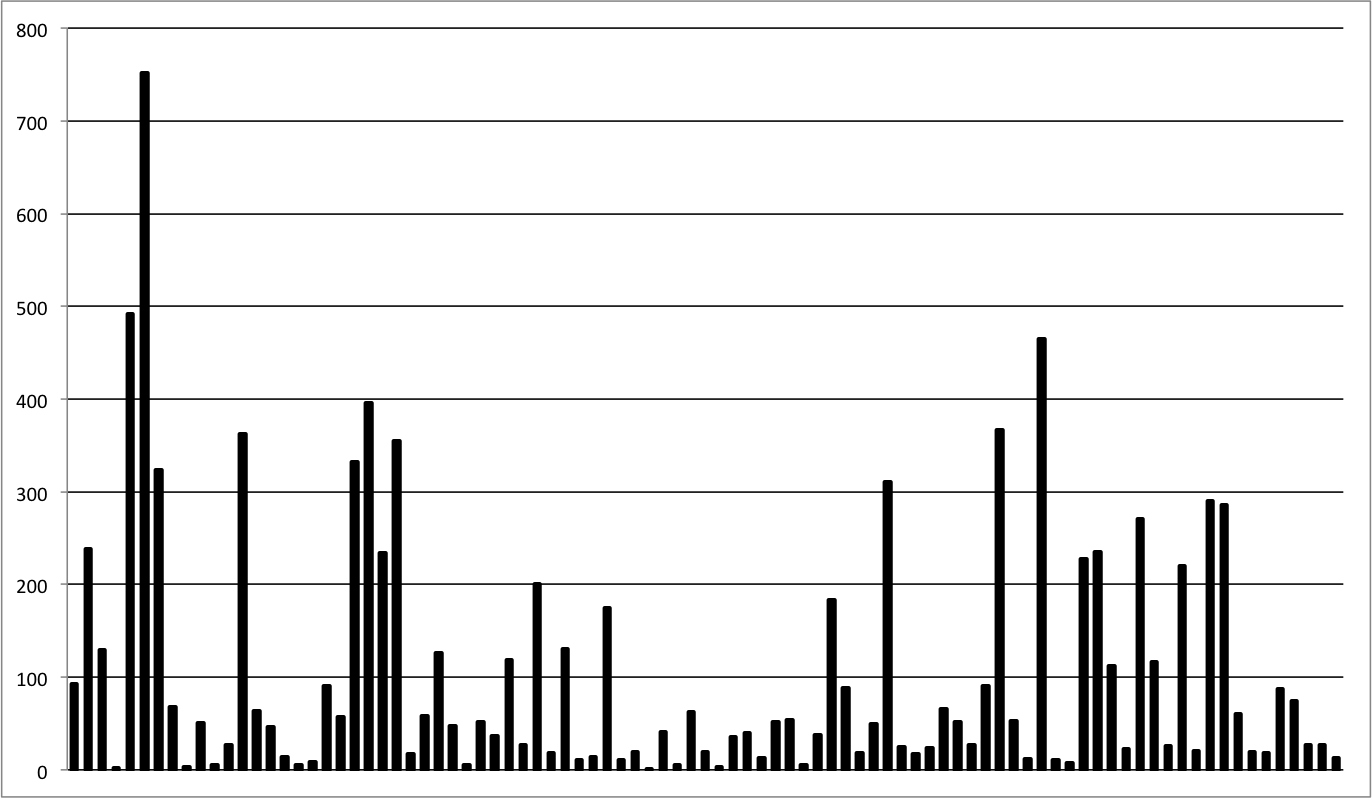
\includegraphics[width=1.00\textwidth]{imgs/ChartCampaignsRecipients.png}
	\caption[Campaigns and Their Number of Recipients in Myriad]{Campaigns and Their Number of Recipients in Myriad}
	\label{fig:ChartCampaignsRecipients}
\end{figure}

\paragraph{Myriad Users and Their Number of Campaigns} Figure \ref{fig:ChartUsersCampaigns} shows Myriad's total number of users\footnote{Users' names are removed due to privacy reasons.}, and the number of campaigns that they created with Myriad. There are a total 96 campaigns, after the ones created for test purposes were ignored. The average was 3.92 campaigns per user. While the maximum amount of campaigns created by one user was 13, the minimum amount was one campaign.

\begin{figure}[htbp]
	\centering
	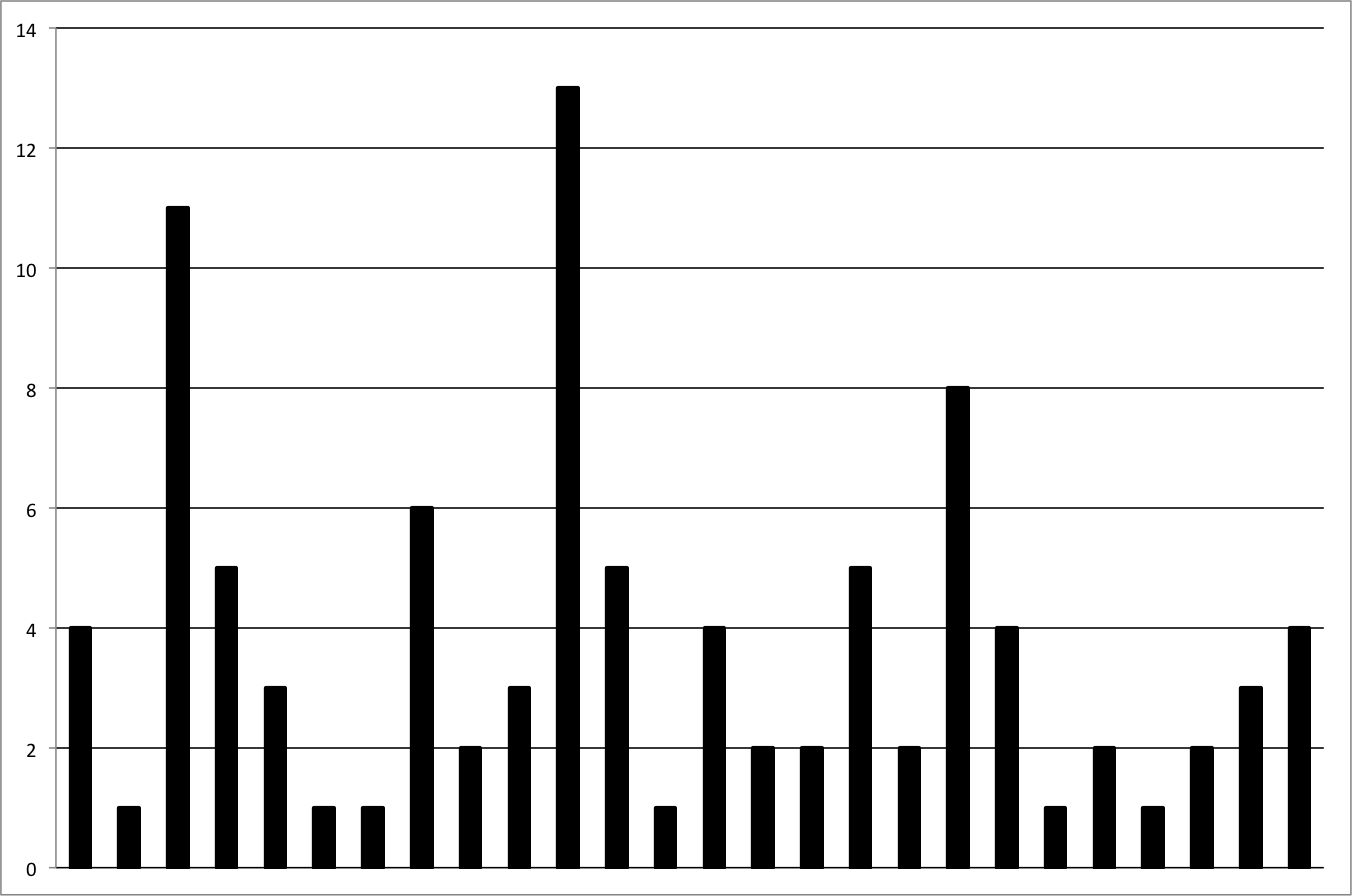
\includegraphics[width=0.85\textwidth]{imgs/ChartUsersCampaigns.png}
	\caption[Myriad Users and Their Number of Campaigns]{Myriad Users and Their Number of Campaigns}
	\label{fig:ChartUsersCampaigns}
\end{figure}

\paragraph{The Number of Campaigns per Month} Figure \ref{fig:ChartCampaignsMonths} shows the ratio of created campaigns per month. 35 campaigns out of 96 were created in April 2013, as the highest amount compared to other months. It might be because it is the middle of spring quarter at Stanford University, where lecturers and organizations need to reach their recipients more often. There were an average of 15.5 campaigns created per month if the launched month January is ignored.

\begin{figure}[htbp]
	\centering
	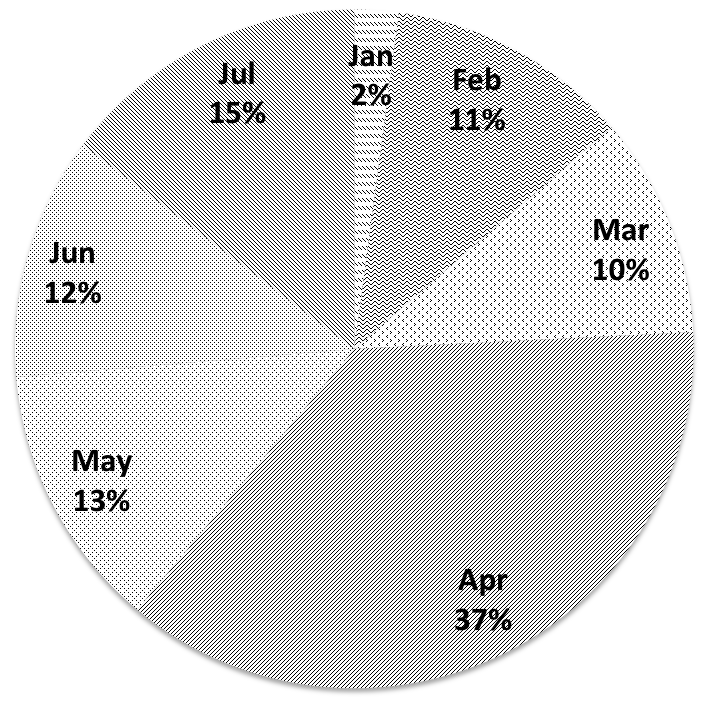
\includegraphics[width=0.50\textwidth]{imgs/ChartCampaignsMonths.png}
	\caption[The Number of Campaigns per Month]{The Number of Campaigns per Month}
	\label{fig:ChartCampaignsMonths}
\end{figure}

\subsection{User Testimonials}
\label{subsec:5.4.2:UserTest}

In this section, testimonials from the very active users of Myriad will be evaluated. Users were asked to evaluate Myriad, keeping the following four questions in mind:

\begin{compactenum}
	\item What are the scenarios you use Myriad for?
	\item What were you using before Myriad?
	\item How satisfied are you with Myriad?
	\item How regularly do you use Myriad?
\end{compactenum}
\vspace{1cm}

Testimonials written in listing \ref{lst:Testimonial1} and \ref{lst:Testimonial2} belongs to lecturers from the Stanford \ac{HCI} group. The last testimonial belongs to a Stanford organization who performs mass email communication very often to reach their community.

\vspace{1cm}

\lstset {
 basicstyle=,
 frame=shadowbox,
 rulesepcolor=\color{black},
 showspaces=false,showtabs=false,tabsize=4,
 numberstyle=\tiny,
 captionpos=b,
 xleftmargin=0.7cm, xrightmargin=0.5cm,
 lineskip=-0.1em,
 abovecaptionskip=1\baselineskip
}

\begin{lstlisting}[language=, caption={[User Testimonial about Myriad \#1]User Testimonial about Myriad \#1}, label={lst:Testimonial1}]

My main use: handling a special issue. Several hundred emails (literally) meant that an email view was impossible. Myriad's structured view makes everything a whole lot easier. It still needs some polishing to be ready for prime time (like it's workflow emphasis is a little constrained, and it needs better handing of formatting and attachments), but as a first draft, it's amazing. I hope it continues so I can use it more!

- Prof. Scott R. Klemmer, Stanford HCI Group
\end{lstlisting}

\vspace{1cm}

\begin{lstlisting}[language=, caption={[User Testimonial about Myriad \#2]User Testimonial about Myriad \#2}, label={lst:Testimonial2}]

I use Myriad to manage a large volume of emails about the courses that I'm teaching. I tag the email with the campaign, and the system+assistant help me respond with one of a number of common responses.

- Prof. Michael S. Bernstein, Stanford HCI Group
\end{lstlisting}

\clearpage

\begin{lstlisting}[language=, caption={[User Testimonial about Myriad \#3]User Testimonial about Myriad \#3}, label={lst:Testimonial3}]

I use Myriad when I'm mass-mailing a group of people and want to personalize the email. Before, I was using Mailchimp or BCC everyone. It's a great tool to send personalized emails to the network! I use Myriad whenever I need to email more than 10 people and want to personalize the emails. For less than 10, the set up for Myriad may take longer than sending out the emails individually (this was discovered through trial and error).
\end{lstlisting}

\section{Conclusion}
\label{sec:5.5:Conc}

In this section, the final solution, Myriad, for personalized mass email communication was investigated. We first investigated the improved requirements, comparing them with the initial requirements, and the ones already applied to the initial prototype. Enabling assistant support, using \ac{KVP}s as dynamic variables in the email, importing recipients list from a Google Spreadsheet, the ability to import email from Gmail's inbox by annotating emails using Myriad's campaign labels, and automated decision-making through previously applied search filters were some of the main improvements done in Myriad.
\vspace{1cm}

Previous sections continued showing how those features were applied for Myriad's \ac{UI}, followed by introducing its architecture on how it was possible to enable the said features in support for mass email communication.
\vspace{1cm}

Finally, user and campaign statistics were given to show how actively Myriad was used during its beta stage, and the section was followed by testimonials from the active users of Myriad.
\vspace{1cm}

After discussing what Myriad is, its features, and users' testimonials, let us see how these features fit into a personalized mass email communication. A personalized mass email communication can be illustrated as shown in figure \ref{fig:drawingStatesOfEmailCommunication}.
\vspace{1cm}

\begin{figure}[htbp]
	\centering
	\begin{pdfpic}
	    %LaTeX with PSTricks extensions
%%Creator: inkscape 0.48.2
%%Please note this file requires PSTricks extensions
\psset{xunit=.5pt,yunit=.5pt,runit=.5pt}
\begin{pspicture}(744.09448242,1052.36218262)
{
\newrgbcolor{curcolor}{1 1 1}
\pscustom[linestyle=none,fillstyle=solid,fillcolor=curcolor]
{
\newpath
\moveto(97.28740472,803.6705408)
\curveto(97.28740472,793.27704029)(90.76308552,784.85144338)(82.71492993,784.85144338)
\curveto(74.66677433,784.85144338)(68.14245513,793.27704029)(68.14245513,803.6705408)
\curveto(68.14245513,814.06404132)(74.66677433,822.48963823)(82.71492993,822.48963823)
\curveto(90.76308552,822.48963823)(97.28740472,814.06404132)(97.28740472,803.6705408)
\closepath
}
}
{
\newrgbcolor{curcolor}{0 0 0}
\pscustom[linewidth=0.88329015,linecolor=curcolor]
{
\newpath
\moveto(97.28740472,803.6705408)
\curveto(97.28740472,793.27704029)(90.76308552,784.85144338)(82.71492993,784.85144338)
\curveto(74.66677433,784.85144338)(68.14245513,793.27704029)(68.14245513,803.6705408)
\curveto(68.14245513,814.06404132)(74.66677433,822.48963823)(82.71492993,822.48963823)
\curveto(90.76308552,822.48963823)(97.28740472,814.06404132)(97.28740472,803.6705408)
\closepath
}
}
{
\newrgbcolor{curcolor}{0 0 0}
\pscustom[linewidth=1.01820959,linecolor=curcolor]
{
\newpath
\moveto(82.69688954,784.93184091)
\lineto(82.09555619,716.9047674)
}
}
{
\newrgbcolor{curcolor}{0 0 0}
\pscustom[linewidth=1.38009903,linecolor=curcolor]
{
\newpath
\moveto(82.69688954,783.37935355)
\lineto(108.55425018,758.53932063)
}
}
{
\newrgbcolor{curcolor}{0 0 0}
\pscustom[linewidth=1.44034747,linecolor=curcolor]
{
\newpath
\moveto(56.23819554,756.32316606)
\lineto(82.09555497,783.37933787)
}
}
{
\newrgbcolor{curcolor}{0 0 0}
\pscustom[linewidth=1.38009903,linecolor=curcolor]
{
\newpath
\moveto(82.09555862,718.17430437)
\lineto(107.95292048,693.33427145)
}
}
{
\newrgbcolor{curcolor}{0 0 0}
\pscustom[linewidth=1.44034747,linecolor=curcolor]
{
\newpath
\moveto(56.23819554,691.89435271)
\lineto(82.09555497,718.95052453)
}
}
{
\newrgbcolor{curcolor}{1 1 1}
\pscustom[linestyle=none,fillstyle=solid,fillcolor=curcolor]
{
\newpath
\moveto(178.63246872,927.2600828)
\curveto(178.63246872,916.86658229)(172.10814952,908.44098538)(164.05999393,908.44098538)
\curveto(156.01183833,908.44098538)(149.48751913,916.86658229)(149.48751913,927.2600828)
\curveto(149.48751913,937.65358332)(156.01183833,946.07918023)(164.05999393,946.07918023)
\curveto(172.10814952,946.07918023)(178.63246872,937.65358332)(178.63246872,927.2600828)
\closepath
}
}
{
\newrgbcolor{curcolor}{0 0 0}
\pscustom[linewidth=0.88329015,linecolor=curcolor]
{
\newpath
\moveto(178.63246872,927.2600828)
\curveto(178.63246872,916.86658229)(172.10814952,908.44098538)(164.05999393,908.44098538)
\curveto(156.01183833,908.44098538)(149.48751913,916.86658229)(149.48751913,927.2600828)
\curveto(149.48751913,937.65358332)(156.01183833,946.07918023)(164.05999393,946.07918023)
\curveto(172.10814952,946.07918023)(178.63246872,937.65358332)(178.63246872,927.2600828)
\closepath
}
}
{
\newrgbcolor{curcolor}{0 0 0}
\pscustom[linewidth=1.01820959,linecolor=curcolor]
{
\newpath
\moveto(164.04195354,908.52138291)
\lineto(163.44062019,840.4943094)
}
}
{
\newrgbcolor{curcolor}{0 0 0}
\pscustom[linewidth=1.38009903,linecolor=curcolor]
{
\newpath
\moveto(164.04195354,906.96889555)
\lineto(189.89931418,882.12886263)
}
}
{
\newrgbcolor{curcolor}{0 0 0}
\pscustom[linewidth=1.44034747,linecolor=curcolor]
{
\newpath
\moveto(137.58325954,879.91270806)
\lineto(163.44061897,906.96887987)
}
}
{
\newrgbcolor{curcolor}{0 0 0}
\pscustom[linewidth=1.38009903,linecolor=curcolor]
{
\newpath
\moveto(163.44062262,841.76384637)
\lineto(189.29798448,816.92381345)
}
}
{
\newrgbcolor{curcolor}{0 0 0}
\pscustom[linewidth=1.44034747,linecolor=curcolor]
{
\newpath
\moveto(137.58325954,815.48389471)
\lineto(163.44061897,842.54006653)
}
}
{
\newrgbcolor{curcolor}{1 1 1}
\pscustom[linestyle=none,fillstyle=solid,fillcolor=curcolor]
{
\newpath
\moveto(180.22745972,685.6987448)
\curveto(180.22745972,675.30524429)(173.70314052,666.87964738)(165.65498493,666.87964738)
\curveto(157.60682933,666.87964738)(151.08251013,675.30524429)(151.08251013,685.6987448)
\curveto(151.08251013,696.09224532)(157.60682933,704.51784223)(165.65498493,704.51784223)
\curveto(173.70314052,704.51784223)(180.22745972,696.09224532)(180.22745972,685.6987448)
\closepath
}
}
{
\newrgbcolor{curcolor}{0 0 0}
\pscustom[linewidth=0.88329015,linecolor=curcolor]
{
\newpath
\moveto(180.22745972,685.6987448)
\curveto(180.22745972,675.30524429)(173.70314052,666.87964738)(165.65498493,666.87964738)
\curveto(157.60682933,666.87964738)(151.08251013,675.30524429)(151.08251013,685.6987448)
\curveto(151.08251013,696.09224532)(157.60682933,704.51784223)(165.65498493,704.51784223)
\curveto(173.70314052,704.51784223)(180.22745972,696.09224532)(180.22745972,685.6987448)
\closepath
}
}
{
\newrgbcolor{curcolor}{0 0 0}
\pscustom[linewidth=1.01820959,linecolor=curcolor]
{
\newpath
\moveto(165.63694454,666.96004491)
\lineto(165.03561119,598.9329714)
}
}
{
\newrgbcolor{curcolor}{0 0 0}
\pscustom[linewidth=1.38009903,linecolor=curcolor]
{
\newpath
\moveto(165.63694454,665.40755755)
\lineto(191.49430518,640.56752463)
}
}
{
\newrgbcolor{curcolor}{0 0 0}
\pscustom[linewidth=1.44034747,linecolor=curcolor]
{
\newpath
\moveto(139.17825054,638.35137006)
\lineto(165.03560997,665.40754187)
}
}
{
\newrgbcolor{curcolor}{0 0 0}
\pscustom[linewidth=1.38009903,linecolor=curcolor]
{
\newpath
\moveto(165.03561362,600.20250837)
\lineto(190.89297548,575.36247545)
}
}
{
\newrgbcolor{curcolor}{0 0 0}
\pscustom[linewidth=1.44034747,linecolor=curcolor]
{
\newpath
\moveto(139.17825054,573.92255671)
\lineto(165.03560997,600.97872853)
}
}
{
\newrgbcolor{curcolor}{0 0 0}
\pscustom[linewidth=1.98745421,linecolor=curcolor]
{
\newpath
\moveto(393.33032186,773.22187148)
\curveto(393.33032186,716.34138031)(384.76104564,670.23063157)(374.19030772,670.23063157)
\curveto(363.6195698,670.23063157)(355.05029358,716.34138031)(355.05029358,773.22187148)
\curveto(355.05029358,830.10236264)(363.6195698,876.21311138)(374.19030772,876.21311138)
\curveto(384.76104564,876.21311138)(393.33032186,830.10236264)(393.33032186,773.22187148)
\closepath
}
}
{
\newrgbcolor{curcolor}{0 0 0}
\pscustom[linewidth=1.98745425,linecolor=curcolor]
{
\newpath
\moveto(374.19030588,876.21309029)
\lineto(468.29537325,814.41834763)
\lineto(536.88042669,814.41834763)
\lineto(536.88042669,747.00590109)
\lineto(471.4853686,748.87846905)
\lineto(377.38031402,672.10316739)
}
}
{
\newrgbcolor{curcolor}{0 0 0}
\pscustom[linewidth=1.17573655,linecolor=curcolor]
{
\newpath
\moveto(196.47594,878.55306262)
\lineto(310.38827,823.92326262)
}
}
{
\newrgbcolor{curcolor}{0 0 0}
\pscustom[linestyle=none,fillstyle=solid,fillcolor=curcolor]
{
\newpath
\moveto(301.31091269,834.06233684)
\lineto(311.80509536,823.2667535)
\lineto(296.81704938,824.69187709)
\curveto(300.17913394,826.48185581)(301.98240688,830.27206431)(301.31091269,834.06233684)
\closepath
}
}
{
\newrgbcolor{curcolor}{0 0 0}
\pscustom[linewidth=1.17321301,linecolor=curcolor]
{
\newpath
\moveto(111.91755,755.93626262)
\lineto(308.68429,754.52521262)
}
}
{
\newrgbcolor{curcolor}{0 0 0}
\pscustom[linestyle=none,fillstyle=solid,fillcolor=curcolor]
{
\newpath
\moveto(296.1797714,759.8206923)
\lineto(310.24244665,754.53470498)
\lineto(296.10540728,749.45094408)
\curveto(298.37992696,752.49593777)(298.39698182,756.68421158)(296.1797714,759.8206923)
\closepath
}
}
{
\newrgbcolor{curcolor}{0 0 0}
\pscustom[linewidth=1.17902207,linecolor=curcolor]
{
\newpath
\moveto(196.09019,640.54195262)
\lineto(324.02591,715.67676262)
}
}
{
\newrgbcolor{curcolor}{0 0 0}
\pscustom[linestyle=none,fillstyle=solid,fillcolor=curcolor]
{
\newpath
\moveto(310.50808167,713.80484856)
\lineto(325.36553761,716.4875913)
\lineto(315.78557941,704.81859319)
\curveto(316.17970156,708.61773769)(314.03695398,712.24054132)(310.50808167,713.80484856)
\closepath
}
}
{
\newrgbcolor{curcolor}{1 1 1}
\pscustom[linestyle=none,fillstyle=solid,fillcolor=curcolor]
{
\newpath
\moveto(709.12200872,837.6294918)
\curveto(709.12200872,827.23599129)(702.59768952,818.81039438)(694.54953393,818.81039438)
\curveto(686.50137833,818.81039438)(679.97705913,827.23599129)(679.97705913,837.6294918)
\curveto(679.97705913,848.02299232)(686.50137833,856.44858923)(694.54953393,856.44858923)
\curveto(702.59768952,856.44858923)(709.12200872,848.02299232)(709.12200872,837.6294918)
\closepath
}
}
{
\newrgbcolor{curcolor}{0 0 0}
\pscustom[linewidth=0.88329015,linecolor=curcolor]
{
\newpath
\moveto(709.12200872,837.6294918)
\curveto(709.12200872,827.23599129)(702.59768952,818.81039438)(694.54953393,818.81039438)
\curveto(686.50137833,818.81039438)(679.97705913,827.23599129)(679.97705913,837.6294918)
\curveto(679.97705913,848.02299232)(686.50137833,856.44858923)(694.54953393,856.44858923)
\curveto(702.59768952,856.44858923)(709.12200872,848.02299232)(709.12200872,837.6294918)
\closepath
}
}
{
\newrgbcolor{curcolor}{0 0 0}
\pscustom[linewidth=1.01820959,linecolor=curcolor]
{
\newpath
\moveto(694.53149354,818.89079191)
\lineto(693.93016019,750.8637184)
}
}
{
\newrgbcolor{curcolor}{0 0 0}
\pscustom[linewidth=1.38009903,linecolor=curcolor]
{
\newpath
\moveto(694.53149354,817.33830455)
\lineto(720.38885418,792.49827163)
}
}
{
\newrgbcolor{curcolor}{0 0 0}
\pscustom[linewidth=1.44034747,linecolor=curcolor]
{
\newpath
\moveto(668.07279954,790.28211706)
\lineto(693.93015897,817.33828887)
}
}
{
\newrgbcolor{curcolor}{0 0 0}
\pscustom[linewidth=1.38009903,linecolor=curcolor]
{
\newpath
\moveto(693.93016262,752.13325537)
\lineto(719.78752448,727.29322245)
}
}
{
\newrgbcolor{curcolor}{0 0 0}
\pscustom[linewidth=1.44034747,linecolor=curcolor]
{
\newpath
\moveto(668.07279954,725.85330371)
\lineto(693.93015897,752.90947553)
}
}
{
\newrgbcolor{curcolor}{0 0 0}
\pscustom[linewidth=1.02203012,linecolor=curcolor]
{
\newpath
\moveto(722.89553,793.42997262)
\lineto(783.62888,880.34816262)
}
}
{
\newrgbcolor{curcolor}{0 0 0}
\pscustom[linestyle=none,fillstyle=solid,fillcolor=curcolor]
{
\newpath
\moveto(773.65352352,873.98940702)
\lineto(784.391529,881.47105425)
\lineto(781.05860312,868.81516947)
\curveto(779.99659841,871.95117088)(776.99932492,874.03169648)(773.65352352,873.98940702)
\closepath
}
}
{
\newrgbcolor{curcolor}{0 0 0}
\pscustom[linewidth=1.01625431,linecolor=curcolor]
{
\newpath
\moveto(724.31018,792.21185262)
\lineto(787.39081,794.77510262)
}
}
{
\newrgbcolor{curcolor}{0 0 0}
\pscustom[linestyle=none,fillstyle=solid,fillcolor=curcolor]
{
\newpath
\moveto(776.35247656,798.83951748)
\lineto(788.73857484,794.84778404)
\lineto(776.7171808,789.86426529)
\curveto(778.55916836,792.59298063)(778.40063578,796.21748951)(776.35247656,798.83951748)
\closepath
}
}
{
\newrgbcolor{curcolor}{0 0 0}
\pscustom[linewidth=0.95299476,linecolor=curcolor]
{
\newpath
\moveto(721.70083,790.09977262)
\lineto(784.69102,715.87594262)
}
}
{
\newrgbcolor{curcolor}{0 0 0}
\pscustom[linestyle=none,fillstyle=solid,fillcolor=curcolor]
{
\newpath
\moveto(781.32293447,726.37978361)
\lineto(785.52272375,714.92185645)
\lineto(774.90046092,720.92934043)
\curveto(777.98034564,721.14318896)(780.56746102,723.35257748)(781.32293447,726.37978361)
\closepath
}
}
{
\newrgbcolor{curcolor}{1 1 1}
\pscustom[linestyle=none,fillstyle=solid,fillcolor=curcolor]
{
\newpath
\moveto(324.56238738,870.13326608)
\lineto(357.39147353,889.0852063)
\lineto(378.89218415,837.75050106)
\lineto(346.063098,818.79856085)
\closepath
}
}
{
\newrgbcolor{curcolor}{0 0 0}
\pscustom[linewidth=0.71264592,linecolor=curcolor]
{
\newpath
\moveto(324.56238738,870.13326608)
\lineto(357.39147353,889.0852063)
\lineto(378.89218415,837.75050106)
\lineto(346.063098,818.79856085)
\closepath
}
}
{
\newrgbcolor{curcolor}{0 0 0}
\pscustom[linewidth=0.71966339,linecolor=curcolor]
{
\newpath
\moveto(332.75870489,857.7099982)
\curveto(360.6687383,874.2031123)(361.17868456,874.11660035)(361.17868456,874.11660035)
}
}
{
\newrgbcolor{curcolor}{0 0 0}
\pscustom[linewidth=0.71966339,linecolor=curcolor]
{
\newpath
\moveto(334.77488335,852.71622948)
\curveto(362.68491676,869.20934358)(363.19486302,869.12283163)(363.19486302,869.12283163)
}
}
{
\newrgbcolor{curcolor}{0 0 0}
\pscustom[linewidth=0.71966339,linecolor=curcolor]
{
\newpath
\moveto(336.79106806,847.72244586)
\curveto(364.70110147,864.21555996)(365.21104773,864.12904801)(365.21104773,864.12904801)
}
}
{
\newrgbcolor{curcolor}{0 0 0}
\pscustom[linewidth=0.71966339,linecolor=curcolor]
{
\newpath
\moveto(339.23218589,842.97395386)
\curveto(367.1422193,859.46706796)(367.65216214,859.38055404)(367.65216214,859.38055404)
}
}
{
\newrgbcolor{curcolor}{0 0 0}
\pscustom[linewidth=0.71966339,linecolor=curcolor]
{
\newpath
\moveto(341.24837342,837.98015336)
\curveto(369.15840891,854.47326249)(369.66834967,854.38675354)(369.66834967,854.38675354)
}
}
{
\newrgbcolor{curcolor}{0 0 0}
\pscustom[linewidth=0.71966339,linecolor=curcolor]
{
\newpath
\moveto(343.26455813,832.98636973)
\curveto(371.17459362,849.47947887)(371.68453438,849.39296991)(371.68453438,849.39296991)
}
}
{
\newrgbcolor{curcolor}{0 0 0}
\pscustom[linewidth=0.37680256,linecolor=curcolor]
{
\newpath
\moveto(345.15312183,827.91891781)
\curveto(352.71106309,832.66294966)(352.94411249,832.4165876)(352.94411249,832.4165876)
}
}
{
\newrgbcolor{curcolor}{0 0 0}
\pscustom[linewidth=0.37680256,linecolor=curcolor]
{
\newpath
\moveto(330.92149927,862.61798149)
\curveto(338.47944054,867.36201334)(338.71248993,867.11565129)(338.71248993,867.11565129)
}
}
{
\newrgbcolor{curcolor}{1 1 1}
\pscustom[linestyle=none,fillstyle=solid,fillcolor=curcolor]
{
\newpath
\moveto(317.13503459,756.98482481)
\lineto(328.95341269,797.63150548)
\lineto(375.06649955,779.15115866)
\lineto(363.24812145,738.50447799)
\closepath
}
}
{
\newrgbcolor{curcolor}{0 0 0}
\pscustom[linewidth=0.71264592,linecolor=curcolor]
{
\newpath
\moveto(317.13503459,756.98482481)
\lineto(328.95341269,797.63150548)
\lineto(375.06649955,779.15115866)
\lineto(363.24812145,738.50447799)
\closepath
}
}
{
\newrgbcolor{curcolor}{0 0 0}
\pscustom[linewidth=0.71966339,linecolor=curcolor]
{
\newpath
\moveto(330.41221934,754.99579026)
\curveto(340.23046723,789.82153051)(340.64333159,790.18342335)(340.64333159,790.18342335)
}
}
{
\newrgbcolor{curcolor}{0 0 0}
\pscustom[linewidth=0.71966339,linecolor=curcolor]
{
\newpath
\moveto(334.84470427,753.13550474)
\curveto(344.66295216,787.96124499)(345.07581652,788.32313784)(345.07581652,788.32313784)
}
}
{
\newrgbcolor{curcolor}{0 0 0}
\pscustom[linewidth=0.71966339,linecolor=curcolor]
{
\newpath
\moveto(339.27720258,751.27521385)
\curveto(349.09545047,786.10095411)(349.50831483,786.46284695)(349.50831483,786.46284695)
}
}
{
\newrgbcolor{curcolor}{0 0 0}
\pscustom[linewidth=0.71966339,linecolor=curcolor]
{
\newpath
\moveto(343.86268676,749.94103238)
\curveto(353.68093465,784.76677264)(354.09379778,785.12866125)(354.09379778,785.12866125)
}
}
{
\newrgbcolor{curcolor}{0 0 0}
\pscustom[linewidth=0.71966339,linecolor=curcolor]
{
\newpath
\moveto(348.29519724,748.0807319)
\curveto(358.11344959,782.90647037)(358.52630825,783.26836076)(358.52630825,783.26836076)
}
}
{
\newrgbcolor{curcolor}{0 0 0}
\pscustom[linewidth=0.71966339,linecolor=curcolor]
{
\newpath
\moveto(352.72769555,746.22044101)
\curveto(362.54594791,781.04617948)(362.95880657,781.40806988)(362.95880657,781.40806988)
}
}
{
\newrgbcolor{curcolor}{0 0 0}
\pscustom[linewidth=0.37680256,linecolor=curcolor]
{
\newpath
\moveto(357.11424695,744.20214308)
\curveto(359.60579927,753.82934487)(359.91898154,753.84840336)(359.91898154,753.84840336)
}
}
{
\newrgbcolor{curcolor}{0 0 0}
\pscustom[linewidth=0.37680256,linecolor=curcolor]
{
\newpath
\moveto(326.15799716,756.94387543)
\curveto(328.64954948,766.57107721)(328.96273175,766.59013571)(328.96273175,766.59013571)
}
}
{
\newrgbcolor{curcolor}{1 1 1}
\pscustom[linestyle=none,fillstyle=solid,fillcolor=curcolor]
{
\newpath
\moveto(329.39229051,685.2904872)
\lineto(334.89598907,727.75127868)
\lineto(383.06716017,719.14516908)
\lineto(377.56346161,676.68437759)
\closepath
}
}
{
\newrgbcolor{curcolor}{0 0 0}
\pscustom[linewidth=0.71264589,linecolor=curcolor]
{
\newpath
\moveto(329.39229051,685.2904872)
\lineto(334.89598907,727.75127868)
\lineto(383.06716017,719.14516908)
\lineto(377.56346161,676.68437759)
\closepath
}
}
{
\newrgbcolor{curcolor}{0 0 0}
\pscustom[linewidth=0.71966336,linecolor=curcolor]
{
\newpath
\moveto(342.75971296,686.09189893)
\curveto(347.17245302,722.4080256)(347.52423794,722.8499989)(347.52423794,722.8499989)
}
}
{
\newrgbcolor{curcolor}{0 0 0}
\pscustom[linewidth=0.71966336,linecolor=curcolor]
{
\newpath
\moveto(347.40267681,685.18207042)
\curveto(351.81541688,721.4981971)(352.1672018,721.94017039)(352.1672018,721.94017039)
}
}
{
\newrgbcolor{curcolor}{0 0 0}
\pscustom[linewidth=0.71966336,linecolor=curcolor]
{
\newpath
\moveto(352.04565465,684.27223942)
\curveto(356.45839472,720.5883661)(356.81017964,721.03033939)(356.81017964,721.03033939)
}
}
{
\newrgbcolor{curcolor}{0 0 0}
\pscustom[linewidth=0.71966336,linecolor=curcolor]
{
\newpath
\moveto(356.7598842,683.91200184)
\curveto(361.17262427,720.22812852)(361.52440862,720.67009739)(361.52440862,720.67009739)
}
}
{
\newrgbcolor{curcolor}{0 0 0}
\pscustom[linewidth=0.71966336,linecolor=curcolor]
{
\newpath
\moveto(361.40287546,683.00216392)
\curveto(365.81562018,719.31828976)(366.16739987,719.76025947)(366.16739987,719.76025947)
}
}
{
\newrgbcolor{curcolor}{0 0 0}
\pscustom[linewidth=0.71966336,linecolor=curcolor]
{
\newpath
\moveto(366.04585329,682.09233292)
\curveto(370.45859802,718.40845876)(370.8103777,718.85042847)(370.8103777,718.85042847)
}
}
{
\newrgbcolor{curcolor}{0 0 0}
\pscustom[linewidth=0.37680254,linecolor=curcolor]
{
\newpath
\moveto(370.66743154,681.01744179)
\curveto(371.66820394,691.01038857)(371.97356793,691.0942264)(371.97356793,691.0942264)
}
}
{
\newrgbcolor{curcolor}{0 0 0}
\pscustom[linewidth=0.37680254,linecolor=curcolor]
{
\newpath
\moveto(338.27896014,687.12518434)
\curveto(339.27973254,697.11813112)(339.58509653,697.20196895)(339.58509653,697.20196895)
}
}
{
\newrgbcolor{curcolor}{1 1 1}
\pscustom[linestyle=none,fillstyle=solid,fillcolor=curcolor]
{
\newpath
\moveto(330.14086178,701.46307564)
\lineto(318.23714202,742.07541628)
\lineto(364.31127092,760.68921383)
\lineto(376.21499068,720.07687319)
\closepath
}
}
{
\newrgbcolor{curcolor}{0 0 0}
\pscustom[linewidth=0.71264592,linecolor=curcolor]
{
\newpath
\moveto(330.14086178,701.46307564)
\lineto(318.23714202,742.07541628)
\lineto(364.31127092,760.68921383)
\lineto(376.21499068,720.07687319)
\closepath
}
}
{
\newrgbcolor{curcolor}{0 0 0}
\pscustom[linewidth=0.71966339,linecolor=curcolor]
{
\newpath
\moveto(341.66592432,709.45392964)
\curveto(331.22395254,744.02869653)(331.36093222,744.61183474)(331.36093222,744.61183474)
}
}
{
\newrgbcolor{curcolor}{0 0 0}
\pscustom[linewidth=0.71966339,linecolor=curcolor]
{
\newpath
\moveto(346.13850994,711.17685216)
\curveto(335.69653816,745.75161905)(335.83351784,746.33475726)(335.83351784,746.33475726)
}
}
{
\newrgbcolor{curcolor}{0 0 0}
\pscustom[linewidth=0.71966339,linecolor=curcolor]
{
\newpath
\moveto(350.61110894,712.89978008)
\curveto(340.16913715,747.47454698)(340.30611683,748.05768518)(340.30611683,748.05768518)
}
}
{
\newrgbcolor{curcolor}{0 0 0}
\pscustom[linewidth=0.71966339,linecolor=curcolor]
{
\newpath
\moveto(354.92964421,715.14838371)
\curveto(344.48767242,749.7231506)(344.62465334,750.30628457)(344.62465334,750.30628457)
}
}
{
\newrgbcolor{curcolor}{0 0 0}
\pscustom[linewidth=0.71966339,linecolor=curcolor]
{
\newpath
\moveto(359.40225782,716.8713128)
\curveto(348.96029049,751.4460815)(349.09726695,752.02921367)(349.09726695,752.02921367)
}
}
{
\newrgbcolor{curcolor}{0 0 0}
\pscustom[linewidth=0.71966339,linecolor=curcolor]
{
\newpath
\moveto(363.87485681,718.59424073)
\curveto(353.43288948,753.16900942)(353.56986595,753.7521416)(353.56986595,753.7521416)
}
}
{
\newrgbcolor{curcolor}{0 0 0}
\pscustom[linewidth=0.37680256,linecolor=curcolor]
{
\newpath
\moveto(368.39372556,720.15929151)
\curveto(365.33135612,729.55680872)(365.56873771,729.79740222)(365.56873771,729.79740222)
}
}
{
\newrgbcolor{curcolor}{0 0 0}
\pscustom[linewidth=0.37680256,linecolor=curcolor]
{
\newpath
\moveto(337.28824952,707.92872591)
\curveto(334.22588009,717.32624313)(334.46326167,717.56683662)(334.46326167,717.56683662)
}
}
{
\newrgbcolor{curcolor}{1 1 1}
\pscustom[linestyle=none,fillstyle=solid,fillcolor=curcolor]
{
\newpath
\moveto(320.20563984,778.27465474)
\lineto(314.80207307,820.75317172)
\lineto(362.99335091,829.20270753)
\lineto(368.39691768,786.72419055)
\closepath
}
}
{
\newrgbcolor{curcolor}{0 0 0}
\pscustom[linewidth=0.71264592,linecolor=curcolor]
{
\newpath
\moveto(320.20563984,778.27465474)
\lineto(314.80207307,820.75317172)
\lineto(362.99335091,829.20270753)
\lineto(368.39691768,786.72419055)
\closepath
}
}
{
\newrgbcolor{curcolor}{0 0 0}
\pscustom[linewidth=0.71966339,linecolor=curcolor]
{
\newpath
\moveto(332.77767936,783.66721468)
\curveto(327.87467585,819.89656961)(328.09983798,820.44065952)(328.09983798,820.44065952)
}
}
{
\newrgbcolor{curcolor}{0 0 0}
\pscustom[linewidth=0.71966339,linecolor=curcolor]
{
\newpath
\moveto(337.44275376,784.40485986)
\curveto(332.53975026,820.6342148)(332.76491238,821.17830471)(332.76491238,821.17830471)
}
}
{
\newrgbcolor{curcolor}{0 0 0}
\pscustom[linewidth=0.71966339,linecolor=curcolor]
{
\newpath
\moveto(342.10784216,785.14250751)
\curveto(337.20483865,821.37186244)(337.43000078,821.91595235)(337.43000078,821.91595235)
}
}
{
\newrgbcolor{curcolor}{0 0 0}
\pscustom[linewidth=0.71966339,linecolor=curcolor]
{
\newpath
\moveto(346.70300289,786.42998296)
\curveto(341.79999938,822.65933789)(342.02516207,823.20342338)(342.02516207,823.20342338)
}
}
{
\newrgbcolor{curcolor}{0 0 0}
\pscustom[linewidth=0.71966339,linecolor=curcolor]
{
\newpath
\moveto(351.36810584,787.16762863)
\curveto(346.46510699,823.39698438)(346.69026502,823.94106905)(346.69026502,823.94106905)
}
}
{
\newrgbcolor{curcolor}{0 0 0}
\pscustom[linewidth=0.71966339,linecolor=curcolor]
{
\newpath
\moveto(356.03319423,787.90527627)
\curveto(351.13019539,824.13463202)(351.35535341,824.67871669)(351.35535341,824.67871669)
}
}
{
\newrgbcolor{curcolor}{0 0 0}
\pscustom[linewidth=0.37680256,linecolor=curcolor]
{
\newpath
\moveto(360.71928365,788.47779322)
\curveto(359.16617201,798.3729795)(359.43691051,798.55878444)(359.43691051,798.55878444)
}
}
{
\newrgbcolor{curcolor}{0 0 0}
\pscustom[linewidth=0.37680256,linecolor=curcolor]
{
\newpath
\moveto(328.2366041,783.1036841)
\curveto(326.68349246,792.99887038)(326.95423096,793.18467532)(326.95423096,793.18467532)
}
}
{
\newrgbcolor{curcolor}{1 1 1}
\pscustom[linestyle=none,fillstyle=solid,fillcolor=curcolor]
{
\newpath
\moveto(550.61999016,848.19510017)
\lineto(587.20327572,848.19510017)
\lineto(587.20327572,790.98996905)
\lineto(550.61999016,790.98996905)
\closepath
}
}
{
\newrgbcolor{curcolor}{0 0 0}
\pscustom[linewidth=0.71264592,linecolor=curcolor]
{
\newpath
\moveto(550.61999016,848.19510017)
\lineto(587.20327572,848.19510017)
\lineto(587.20327572,790.98996905)
\lineto(550.61999016,790.98996905)
\closepath
}
}
{
\newrgbcolor{curcolor}{0 0 0}
\pscustom[linewidth=0.71966339,linecolor=curcolor]
{
\newpath
\moveto(553.30587608,832.80062032)
\curveto(584.55074836,833.14243159)(584.97584786,832.80062032)(584.97584786,832.80062032)
}
}
{
\newrgbcolor{curcolor}{0 0 0}
\pscustom[linewidth=0.71966339,linecolor=curcolor]
{
\newpath
\moveto(553.23823094,827.27483568)
\curveto(584.48310322,827.61664695)(584.90820272,827.27483568)(584.90820272,827.27483568)
}
}
{
\newrgbcolor{curcolor}{0 0 0}
\pscustom[linewidth=0.71966339,linecolor=curcolor]
{
\newpath
\moveto(553.1705858,821.74903442)
\curveto(584.41545808,822.09084569)(584.84055758,821.74903442)(584.84055758,821.74903442)
}
}
{
\newrgbcolor{curcolor}{0 0 0}
\pscustom[linewidth=0.71966339,linecolor=curcolor]
{
\newpath
\moveto(553.57646045,816.22321656)
\curveto(584.82133272,816.56502783)(585.24642841,816.22321656)(585.24642841,816.22321656)
}
}
{
\newrgbcolor{curcolor}{0 0 0}
\pscustom[linewidth=0.71966339,linecolor=curcolor]
{
\newpath
\moveto(553.5088115,810.6973987)
\curveto(584.75368377,811.03920444)(585.17877946,810.6973987)(585.17877946,810.6973987)
}
}
{
\newrgbcolor{curcolor}{0 0 0}
\pscustom[linewidth=0.71966339,linecolor=curcolor]
{
\newpath
\moveto(553.44116636,805.17159745)
\curveto(584.68603864,805.51340319)(585.11113432,805.17159745)(585.11113432,805.17159745)
}
}
{
\newrgbcolor{curcolor}{0 0 0}
\pscustom[linewidth=0.37680256,linecolor=curcolor]
{
\newpath
\moveto(553.23130832,799.64580174)
\curveto(561.79670682,799.98761301)(561.91324467,799.64580174)(561.91324467,799.64580174)
}
}
{
\newrgbcolor{curcolor}{0 0 0}
\pscustom[linewidth=0.37680256,linecolor=curcolor]
{
\newpath
\moveto(553.50188506,838.15670616)
\curveto(562.06728356,838.49851744)(562.18382141,838.15670616)(562.18382141,838.15670616)
}
}
{
\newrgbcolor{curcolor}{1 1 1}
\pscustom[linestyle=none,fillstyle=solid,fillcolor=curcolor]
{
\newpath
\moveto(561.31041016,833.00197917)
\lineto(597.89369572,833.00197917)
\lineto(597.89369572,775.79684805)
\lineto(561.31041016,775.79684805)
\closepath
}
}
{
\newrgbcolor{curcolor}{0 0 0}
\pscustom[linewidth=0.71264592,linecolor=curcolor]
{
\newpath
\moveto(561.31041016,833.00197917)
\lineto(597.89369572,833.00197917)
\lineto(597.89369572,775.79684805)
\lineto(561.31041016,775.79684805)
\closepath
}
}
{
\newrgbcolor{curcolor}{0 0 0}
\pscustom[linewidth=0.71966339,linecolor=curcolor]
{
\newpath
\moveto(563.99629608,817.60749932)
\curveto(595.24116836,817.94931059)(595.66626786,817.60749932)(595.66626786,817.60749932)
}
}
{
\newrgbcolor{curcolor}{0 0 0}
\pscustom[linewidth=0.71966339,linecolor=curcolor]
{
\newpath
\moveto(563.92865094,812.08171468)
\curveto(595.17352322,812.42352595)(595.59862272,812.08171468)(595.59862272,812.08171468)
}
}
{
\newrgbcolor{curcolor}{0 0 0}
\pscustom[linewidth=0.71966339,linecolor=curcolor]
{
\newpath
\moveto(563.8610058,806.55591342)
\curveto(595.10587808,806.89772469)(595.53097758,806.55591342)(595.53097758,806.55591342)
}
}
{
\newrgbcolor{curcolor}{0 0 0}
\pscustom[linewidth=0.71966339,linecolor=curcolor]
{
\newpath
\moveto(564.26688045,801.03009556)
\curveto(595.51175272,801.37190683)(595.93684841,801.03009556)(595.93684841,801.03009556)
}
}
{
\newrgbcolor{curcolor}{0 0 0}
\pscustom[linewidth=0.71966339,linecolor=curcolor]
{
\newpath
\moveto(564.1992315,795.5042777)
\curveto(595.44410377,795.84608344)(595.86919946,795.5042777)(595.86919946,795.5042777)
}
}
{
\newrgbcolor{curcolor}{0 0 0}
\pscustom[linewidth=0.71966339,linecolor=curcolor]
{
\newpath
\moveto(564.13158636,789.97847645)
\curveto(595.37645864,790.32028219)(595.80155432,789.97847645)(595.80155432,789.97847645)
}
}
{
\newrgbcolor{curcolor}{0 0 0}
\pscustom[linewidth=0.37680256,linecolor=curcolor]
{
\newpath
\moveto(563.92172832,784.45268074)
\curveto(572.48712682,784.79449201)(572.60366467,784.45268074)(572.60366467,784.45268074)
}
}
{
\newrgbcolor{curcolor}{0 0 0}
\pscustom[linewidth=0.37680256,linecolor=curcolor]
{
\newpath
\moveto(564.19230506,822.96358516)
\curveto(572.75770356,823.30539644)(572.87424141,822.96358516)(572.87424141,822.96358516)
}
}
{
\newrgbcolor{curcolor}{1 1 1}
\pscustom[linestyle=none,fillstyle=solid,fillcolor=curcolor]
{
\newpath
\moveto(572.00081016,817.80885717)
\lineto(608.58409572,817.80885717)
\lineto(608.58409572,760.60372605)
\lineto(572.00081016,760.60372605)
\closepath
}
}
{
\newrgbcolor{curcolor}{0 0 0}
\pscustom[linewidth=0.71264592,linecolor=curcolor]
{
\newpath
\moveto(572.00081016,817.80885717)
\lineto(608.58409572,817.80885717)
\lineto(608.58409572,760.60372605)
\lineto(572.00081016,760.60372605)
\closepath
}
}
{
\newrgbcolor{curcolor}{0 0 0}
\pscustom[linewidth=0.71966339,linecolor=curcolor]
{
\newpath
\moveto(574.68669608,802.41437732)
\curveto(605.93156836,802.75618859)(606.35666786,802.41437732)(606.35666786,802.41437732)
}
}
{
\newrgbcolor{curcolor}{0 0 0}
\pscustom[linewidth=0.71966339,linecolor=curcolor]
{
\newpath
\moveto(574.61905094,796.88859268)
\curveto(605.86392322,797.23040395)(606.28902272,796.88859268)(606.28902272,796.88859268)
}
}
{
\newrgbcolor{curcolor}{0 0 0}
\pscustom[linewidth=0.71966339,linecolor=curcolor]
{
\newpath
\moveto(574.5514058,791.36279142)
\curveto(605.79627808,791.70460269)(606.22137758,791.36279142)(606.22137758,791.36279142)
}
}
{
\newrgbcolor{curcolor}{0 0 0}
\pscustom[linewidth=0.71966339,linecolor=curcolor]
{
\newpath
\moveto(574.95728045,785.83697356)
\curveto(606.20215272,786.17878483)(606.62724841,785.83697356)(606.62724841,785.83697356)
}
}
{
\newrgbcolor{curcolor}{0 0 0}
\pscustom[linewidth=0.71966339,linecolor=curcolor]
{
\newpath
\moveto(574.8896315,780.3111557)
\curveto(606.13450377,780.65296144)(606.55959946,780.3111557)(606.55959946,780.3111557)
}
}
{
\newrgbcolor{curcolor}{0 0 0}
\pscustom[linewidth=0.71966339,linecolor=curcolor]
{
\newpath
\moveto(574.82198636,774.78535445)
\curveto(606.06685864,775.12716019)(606.49195432,774.78535445)(606.49195432,774.78535445)
}
}
{
\newrgbcolor{curcolor}{0 0 0}
\pscustom[linewidth=0.37680256,linecolor=curcolor]
{
\newpath
\moveto(574.61212832,769.25955874)
\curveto(583.17752682,769.60137001)(583.29406467,769.25955874)(583.29406467,769.25955874)
}
}
{
\newrgbcolor{curcolor}{0 0 0}
\pscustom[linewidth=0.37680256,linecolor=curcolor]
{
\newpath
\moveto(574.88270506,807.77046316)
\curveto(583.44810356,808.11227444)(583.56464141,807.77046316)(583.56464141,807.77046316)
}
}
{
\newrgbcolor{curcolor}{1 1 1}
\pscustom[linestyle=none,fillstyle=solid,fillcolor=curcolor]
{
\newpath
\moveto(582.69124016,802.61573517)
\lineto(619.27452572,802.61573517)
\lineto(619.27452572,745.41060405)
\lineto(582.69124016,745.41060405)
\closepath
}
}
{
\newrgbcolor{curcolor}{0 0 0}
\pscustom[linewidth=0.71264592,linecolor=curcolor]
{
\newpath
\moveto(582.69124016,802.61573517)
\lineto(619.27452572,802.61573517)
\lineto(619.27452572,745.41060405)
\lineto(582.69124016,745.41060405)
\closepath
}
}
{
\newrgbcolor{curcolor}{0 0 0}
\pscustom[linewidth=0.71966339,linecolor=curcolor]
{
\newpath
\moveto(585.37712608,787.22125532)
\curveto(616.62199836,787.56306659)(617.04709786,787.22125532)(617.04709786,787.22125532)
}
}
{
\newrgbcolor{curcolor}{0 0 0}
\pscustom[linewidth=0.71966339,linecolor=curcolor]
{
\newpath
\moveto(585.30948094,781.69547068)
\curveto(616.55435322,782.03728195)(616.97945272,781.69547068)(616.97945272,781.69547068)
}
}
{
\newrgbcolor{curcolor}{0 0 0}
\pscustom[linewidth=0.71966339,linecolor=curcolor]
{
\newpath
\moveto(585.2418358,776.16966942)
\curveto(616.48670808,776.51148069)(616.91180758,776.16966942)(616.91180758,776.16966942)
}
}
{
\newrgbcolor{curcolor}{0 0 0}
\pscustom[linewidth=0.71966339,linecolor=curcolor]
{
\newpath
\moveto(585.64771045,770.64385156)
\curveto(616.89258272,770.98566283)(617.31767841,770.64385156)(617.31767841,770.64385156)
}
}
{
\newrgbcolor{curcolor}{0 0 0}
\pscustom[linewidth=0.71966339,linecolor=curcolor]
{
\newpath
\moveto(585.5800615,765.1180337)
\curveto(616.82493377,765.45983944)(617.25002946,765.1180337)(617.25002946,765.1180337)
}
}
{
\newrgbcolor{curcolor}{0 0 0}
\pscustom[linewidth=0.71966339,linecolor=curcolor]
{
\newpath
\moveto(585.51241636,759.59223245)
\curveto(616.75728864,759.93403819)(617.18238432,759.59223245)(617.18238432,759.59223245)
}
}
{
\newrgbcolor{curcolor}{0 0 0}
\pscustom[linewidth=0.37680256,linecolor=curcolor]
{
\newpath
\moveto(585.30255832,754.06643674)
\curveto(593.86795682,754.40824801)(593.98449467,754.06643674)(593.98449467,754.06643674)
}
}
{
\newrgbcolor{curcolor}{0 0 0}
\pscustom[linewidth=0.37680256,linecolor=curcolor]
{
\newpath
\moveto(585.57313506,792.57734116)
\curveto(594.13853356,792.91915244)(594.25507141,792.57734116)(594.25507141,792.57734116)
}
}
{
\newrgbcolor{curcolor}{1 1 1}
\pscustom[linestyle=none,fillstyle=solid,fillcolor=curcolor]
{
\newpath
\moveto(593.38165016,787.42261617)
\lineto(629.96493572,787.42261617)
\lineto(629.96493572,730.21748505)
\lineto(593.38165016,730.21748505)
\closepath
}
}
{
\newrgbcolor{curcolor}{0 0 0}
\pscustom[linewidth=0.71264592,linecolor=curcolor]
{
\newpath
\moveto(593.38165016,787.42261617)
\lineto(629.96493572,787.42261617)
\lineto(629.96493572,730.21748505)
\lineto(593.38165016,730.21748505)
\closepath
}
}
{
\newrgbcolor{curcolor}{0 0 0}
\pscustom[linewidth=0.71966339,linecolor=curcolor]
{
\newpath
\moveto(596.06753608,772.02813632)
\curveto(627.31240836,772.36994759)(627.73750786,772.02813632)(627.73750786,772.02813632)
}
}
{
\newrgbcolor{curcolor}{0 0 0}
\pscustom[linewidth=0.71966339,linecolor=curcolor]
{
\newpath
\moveto(595.99989094,766.50235168)
\curveto(627.24476322,766.84416295)(627.66986272,766.50235168)(627.66986272,766.50235168)
}
}
{
\newrgbcolor{curcolor}{0 0 0}
\pscustom[linewidth=0.71966339,linecolor=curcolor]
{
\newpath
\moveto(595.9322458,760.97655042)
\curveto(627.17711808,761.31836169)(627.60221758,760.97655042)(627.60221758,760.97655042)
}
}
{
\newrgbcolor{curcolor}{0 0 0}
\pscustom[linewidth=0.71966339,linecolor=curcolor]
{
\newpath
\moveto(596.33812045,755.45073256)
\curveto(627.58299272,755.79254383)(628.00808841,755.45073256)(628.00808841,755.45073256)
}
}
{
\newrgbcolor{curcolor}{0 0 0}
\pscustom[linewidth=0.71966339,linecolor=curcolor]
{
\newpath
\moveto(596.2704715,749.9249147)
\curveto(627.51534377,750.26672044)(627.94043946,749.9249147)(627.94043946,749.9249147)
}
}
{
\newrgbcolor{curcolor}{0 0 0}
\pscustom[linewidth=0.71966339,linecolor=curcolor]
{
\newpath
\moveto(596.20282636,744.39911345)
\curveto(627.44769864,744.74091919)(627.87279432,744.39911345)(627.87279432,744.39911345)
}
}
{
\newrgbcolor{curcolor}{0 0 0}
\pscustom[linewidth=0.37680256,linecolor=curcolor]
{
\newpath
\moveto(595.99296832,738.87331774)
\curveto(604.55836682,739.21512901)(604.67490467,738.87331774)(604.67490467,738.87331774)
}
}
{
\newrgbcolor{curcolor}{0 0 0}
\pscustom[linewidth=0.37680256,linecolor=curcolor]
{
\newpath
\moveto(596.26354506,777.38422216)
\curveto(604.82894356,777.72603344)(604.94548141,777.38422216)(604.94548141,777.38422216)
}
}
{
\newrgbcolor{curcolor}{1 1 1}
\pscustom[linestyle=none,fillstyle=solid,fillcolor=curcolor]
{
\newpath
\moveto(788.66618016,916.44415717)
\lineto(825.24946572,916.44415717)
\lineto(825.24946572,859.23902605)
\lineto(788.66618016,859.23902605)
\closepath
}
}
{
\newrgbcolor{curcolor}{0 0 0}
\pscustom[linewidth=0.71264592,linecolor=curcolor]
{
\newpath
\moveto(788.66618016,916.44415717)
\lineto(825.24946572,916.44415717)
\lineto(825.24946572,859.23902605)
\lineto(788.66618016,859.23902605)
\closepath
}
}
{
\newrgbcolor{curcolor}{0 0 0}
\pscustom[linewidth=0.71966339,linecolor=curcolor]
{
\newpath
\moveto(791.35206608,901.04967732)
\curveto(822.59693836,901.39148859)(823.02203786,901.04967732)(823.02203786,901.04967732)
}
}
{
\newrgbcolor{curcolor}{0 0 0}
\pscustom[linewidth=0.71966339,linecolor=curcolor]
{
\newpath
\moveto(791.28442094,895.52389268)
\curveto(822.52929322,895.86570395)(822.95439272,895.52389268)(822.95439272,895.52389268)
}
}
{
\newrgbcolor{curcolor}{0 0 0}
\pscustom[linewidth=0.71966339,linecolor=curcolor]
{
\newpath
\moveto(791.2167758,889.99809142)
\curveto(822.46164808,890.33990269)(822.88674758,889.99809142)(822.88674758,889.99809142)
}
}
{
\newrgbcolor{curcolor}{0 0 0}
\pscustom[linewidth=0.71966339,linecolor=curcolor]
{
\newpath
\moveto(791.62265045,884.47227356)
\curveto(822.86752272,884.81408483)(823.29261841,884.47227356)(823.29261841,884.47227356)
}
}
{
\newrgbcolor{curcolor}{0 0 0}
\pscustom[linewidth=0.71966339,linecolor=curcolor]
{
\newpath
\moveto(791.5550015,878.9464557)
\curveto(822.79987377,879.28826144)(823.22496946,878.9464557)(823.22496946,878.9464557)
}
}
{
\newrgbcolor{curcolor}{0 0 0}
\pscustom[linewidth=0.71966339,linecolor=curcolor]
{
\newpath
\moveto(791.48735636,873.42065445)
\curveto(822.73222864,873.76246019)(823.15732432,873.42065445)(823.15732432,873.42065445)
}
}
{
\newrgbcolor{curcolor}{0 0 0}
\pscustom[linewidth=0.37680256,linecolor=curcolor]
{
\newpath
\moveto(791.27749832,867.89485874)
\curveto(799.84289682,868.23667001)(799.95943467,867.89485874)(799.95943467,867.89485874)
}
}
{
\newrgbcolor{curcolor}{0 0 0}
\pscustom[linewidth=0.37680256,linecolor=curcolor]
{
\newpath
\moveto(791.54807506,906.40576316)
\curveto(800.11347356,906.74757444)(800.23001141,906.40576316)(800.23001141,906.40576316)
}
}
{
\newrgbcolor{curcolor}{1 1 1}
\pscustom[linestyle=none,fillstyle=solid,fillcolor=curcolor]
{
\newpath
\moveto(790.24743652,826.87167358)
\lineto(826.83071899,826.87167358)
\lineto(826.83071899,769.66654587)
\lineto(790.24743652,769.66654587)
\closepath
}
}
{
\newrgbcolor{curcolor}{0 0 0}
\pscustom[linewidth=0.71264595,linecolor=curcolor]
{
\newpath
\moveto(790.24743652,826.87167358)
\lineto(826.83071899,826.87167358)
\lineto(826.83071899,769.66654587)
\lineto(790.24743652,769.66654587)
\closepath
}
}
{
\newrgbcolor{curcolor}{0 0 0}
\pscustom[linewidth=0.71966332,linecolor=curcolor]
{
\newpath
\moveto(792.9333,811.47718262)
\curveto(824.17817,811.81901262)(824.60325,811.47718262)(824.60325,811.47718262)
}
}
{
\newrgbcolor{curcolor}{0 0 0}
\pscustom[linewidth=0.71966332,linecolor=curcolor]
{
\newpath
\moveto(792.86564,805.95140262)
\curveto(824.11053,806.29322262)(824.53562,805.95140262)(824.53562,805.95140262)
}
}
{
\newrgbcolor{curcolor}{0 0 0}
\pscustom[linewidth=0.71966332,linecolor=curcolor]
{
\newpath
\moveto(793.23002,794.89978262)
\curveto(824.47488,795.24158262)(824.89999,794.89978262)(824.89999,794.89978262)
}
}
{
\newrgbcolor{curcolor}{0 0 0}
\pscustom[linewidth=0.71966332,linecolor=curcolor]
{
\newpath
\moveto(793.04784,789.53485262)
\curveto(824.2927,789.87666262)(824.7178,789.53485262)(824.7178,789.53485262)
}
}
{
\newrgbcolor{curcolor}{0 0 0}
\pscustom[linewidth=0.37680256,linecolor=curcolor]
{
\newpath
\moveto(793.25405,784.35574262)
\curveto(801.81943,784.69754262)(801.93598,784.35574262)(801.93598,784.35574262)
}
}
{
\newrgbcolor{curcolor}{0 0 0}
\pscustom[linewidth=0.37680256,linecolor=curcolor]
{
\newpath
\moveto(793.12929,816.83327262)
\curveto(801.69471,817.17506262)(801.81124,816.83327262)(801.81124,816.83327262)
}
}
{
\newrgbcolor{curcolor}{1 1 1}
\pscustom[linestyle=none,fillstyle=solid,fillcolor=curcolor]
{
\newpath
\moveto(789.45678711,737.2991333)
\lineto(826.04006958,737.2991333)
\lineto(826.04006958,680.09400558)
\lineto(789.45678711,680.09400558)
\closepath
}
}
{
\newrgbcolor{curcolor}{0 0 0}
\pscustom[linewidth=0.71264595,linecolor=curcolor]
{
\newpath
\moveto(789.45678711,737.2991333)
\lineto(826.04006958,737.2991333)
\lineto(826.04006958,680.09400558)
\lineto(789.45678711,680.09400558)
\closepath
}
}
{
\newrgbcolor{curcolor}{0 0 0}
\pscustom[linewidth=0.71966332,linecolor=curcolor]
{
\newpath
\moveto(792.01138,715.93973262)
\curveto(823.25626,716.28154262)(823.68135,715.93973262)(823.68135,715.93973262)
}
}
{
\newrgbcolor{curcolor}{0 0 0}
\pscustom[linewidth=0.71966332,linecolor=curcolor]
{
\newpath
\moveto(791.92117,710.83783262)
\curveto(823.16605,711.17963262)(823.59115,710.83783262)(823.59115,710.83783262)
}
}
{
\newrgbcolor{curcolor}{0 0 0}
\pscustom[linewidth=0.37680256,linecolor=curcolor]
{
\newpath
\moveto(791.6728,705.92178262)
\curveto(800.23818,706.26358262)(800.35473,705.92178262)(800.35473,705.92178262)
}
}
{
\newrgbcolor{curcolor}{0 0 0}
\pscustom[linewidth=0.37680256,linecolor=curcolor]
{
\newpath
\moveto(791.94336,721.22735262)
\curveto(800.50878,721.56919262)(800.62531,721.22735262)(800.62531,721.22735262)
}
}
{
\newrgbcolor{curcolor}{0 0 0}
\pscustom[linewidth=1.40023422,linecolor=curcolor]
{
\newpath
\moveto(50,934.00000262)
\lineto(50,964.66666662)
\lineto(535.90164,964.66666662)
\lineto(535.90164,934.00000262)
\lineto(535.90164,934.00000262)
}
}
{
\newrgbcolor{curcolor}{0 0 0}
\pscustom[linewidth=1.40023422,linecolor=curcolor]
{
\newpath
\moveto(548.68852,934.00000262)
\lineto(548.68852,964.66666662)
\lineto(830,964.66666662)
\lineto(830,934.00000262)
\lineto(830,934.00000262)
\lineto(830,934.00000262)
\lineto(830,934.00000262)
\lineto(830,934.00000262)
}
}
{
\newrgbcolor{curcolor}{0 0 0}
\pscustom[linestyle=none,fillstyle=solid,fillcolor=curcolor]
{
\newpath
\moveto(217.86095677,994.53147838)
\lineto(219.50052521,994.53147838)
\lineto(219.50052521,980.0000004)
\lineto(217.86095677,980.0000004)
\lineto(217.86095677,994.53147838)
}
}
{
\newrgbcolor{curcolor}{0 0 0}
\pscustom[linestyle=none,fillstyle=solid,fillcolor=curcolor]
{
\newpath
\moveto(230.25511993,986.57955774)
\lineto(230.25511993,980.0000004)
\lineto(228.76165165,980.0000004)
\lineto(228.76165165,986.5211593)
\curveto(228.76164402,987.55285749)(228.59389957,988.32501384)(228.25841778,988.83763068)
\curveto(227.92292174,989.35022984)(227.41968836,989.60653384)(226.74871615,989.60654345)
\curveto(225.94245492,989.60653384)(225.30664931,989.29832017)(224.84129743,988.68190151)
\curveto(224.37593813,988.06546549)(224.14326033,987.22517769)(224.14326334,986.1610356)
\lineto(224.14326334,980.0000004)
\lineto(222.64167839,980.0000004)
\lineto(222.64167839,990.90104215)
\lineto(224.14326334,990.90104215)
\lineto(224.14326334,989.20748745)
\curveto(224.50039369,989.86283784)(224.91975484,990.35273536)(225.40134803,990.67718148)
\curveto(225.8883438,991.00160624)(226.44839384,991.16382396)(227.08149984,991.16383513)
\curveto(228.12583842,991.16382396)(228.9158607,990.77450143)(229.45156906,989.99586637)
\curveto(229.98726078,989.22370002)(230.2551108,988.08493162)(230.25511993,986.57955774)
}
}
{
\newrgbcolor{curcolor}{0 0 0}
\pscustom[linestyle=none,fillstyle=solid,fillcolor=curcolor]
{
\newpath
\moveto(239.79221381,990.48252002)
\lineto(239.79221381,988.80843146)
\curveto(239.37013901,989.08743713)(238.94536675,989.29507581)(238.51789578,989.43134813)
\curveto(238.09582224,989.57409029)(237.66834443,989.64546609)(237.23546106,989.64547574)
\curveto(236.26686654,989.64546609)(235.51472204,989.27560969)(234.9790253,988.53590542)
\curveto(234.44332196,987.80267278)(234.17547194,986.77096807)(234.17547443,985.4407882)
\curveto(234.17547194,984.11059745)(234.44332196,983.07564839)(234.9790253,982.33593791)
\curveto(235.51472204,981.60271148)(236.26686654,981.23609943)(237.23546106,981.23610067)
\curveto(237.66834443,981.23609943)(238.09582224,981.30423087)(238.51789578,981.4404952)
\curveto(238.94536675,981.58324535)(239.37013901,981.79412839)(239.79221381,982.07314494)
\lineto(239.79221381,980.41852253)
\curveto(239.37555012,980.1849286)(238.9426612,980.00973346)(238.49354575,979.89293659)
\curveto(238.04982779,979.77613994)(237.57635553,979.71774156)(237.07312755,979.71774128)
\curveto(235.70411095,979.71774156)(234.61647753,980.23359391)(233.81022404,981.26529988)
\curveto(233.00396629,982.29700333)(232.60083848,983.68883137)(232.6008394,985.4407882)
\curveto(232.60083848,987.21868898)(233.00667185,988.61700574)(233.81834071,989.63574266)
\curveto(234.63541642,990.65446032)(235.75281095,991.16382396)(237.17052766,991.16383513)
\curveto(237.63046665,991.16382396)(238.07958891,991.10542558)(238.51789578,990.98863981)
\curveto(238.95618897,990.87832077)(239.38096123,990.70961434)(239.79221381,990.48252002)
}
}
{
\newrgbcolor{curcolor}{0 0 0}
\pscustom[linestyle=none,fillstyle=solid,fillcolor=curcolor]
{
\newpath
\moveto(245.92842066,989.64547574)
\curveto(245.12757106,989.64546609)(244.49447101,989.26912098)(244.02911861,988.51643927)
\curveto(243.56375983,987.77022924)(243.33108203,986.74501324)(243.33108452,985.4407882)
\curveto(243.33108203,984.13655228)(243.56105427,983.10809193)(244.02100193,982.35540406)
\curveto(244.48635434,981.60920019)(245.12215995,981.23609943)(245.92842066,981.23610067)
\curveto(246.72384896,981.23609943)(247.35424346,981.61244454)(247.81960603,982.36513713)
\curveto(248.28495464,983.11782499)(248.51763243,984.14304099)(248.51764011,985.4407882)
\curveto(248.51763243,986.73203582)(248.28495464,987.75400746)(247.81960603,988.5067062)
\curveto(247.35424346,989.26587662)(246.72384896,989.64546609)(245.92842066,989.64547574)
\moveto(245.92842066,991.16383513)
\curveto(247.22708233,991.16382396)(248.24707686,990.65770467)(248.98840729,989.64547574)
\curveto(249.72972142,988.63322751)(250.10038256,987.2316664)(250.10039182,985.4407882)
\curveto(250.10038256,983.65638783)(249.72972142,982.25482672)(248.98840729,981.23610067)
\curveto(248.24707686,980.22386085)(247.22708233,979.71774156)(245.92842066,979.71774128)
\curveto(244.62433769,979.71774156)(243.60163761,980.22386085)(242.86031735,981.23610067)
\curveto(242.12440416,982.25482672)(241.75644858,983.65638783)(241.7564495,985.4407882)
\curveto(241.75644858,987.2316664)(242.12440416,988.63322751)(242.86031735,989.64547574)
\curveto(243.60163761,990.65770467)(244.62433769,991.16382396)(245.92842066,991.16383513)
}
}
{
\newrgbcolor{curcolor}{0 0 0}
\pscustom[linestyle=none,fillstyle=solid,fillcolor=curcolor]
{
\newpath
\moveto(259.64560154,988.80843146)
\curveto(260.01895959,989.61302255)(260.46537629,990.20673941)(260.98485298,990.58958382)
\curveto(261.5043097,990.97240705)(262.1157653,991.16382396)(262.81922162,991.16383513)
\curveto(263.76615432,991.16382396)(264.49665438,990.76476837)(265.01072398,989.96666715)
\curveto(265.52476557,989.1750347)(265.78179337,988.04599936)(265.78180815,986.57955774)
\lineto(265.78180815,980.0000004)
\lineto(264.2802232,980.0000004)
\lineto(264.2802232,986.5211593)
\curveto(264.28020992,987.56583491)(264.12599324,988.34123561)(263.8175727,988.84736375)
\curveto(263.50912652,989.35347419)(263.03835982,989.60653384)(262.40527118,989.60654345)
\curveto(261.63147082,989.60653384)(261.02001522,989.29832017)(260.57090253,988.68190151)
\curveto(260.12177071,988.06546549)(259.89720958,987.22517769)(259.89721847,986.1610356)
\lineto(259.89721847,980.0000004)
\lineto(258.39563352,980.0000004)
\lineto(258.39563352,986.5211593)
\curveto(258.39562613,987.57232362)(258.24140945,988.34772432)(257.93298302,988.84736375)
\curveto(257.62454274,989.35347419)(257.14836492,989.60653384)(256.50444815,989.60654345)
\curveto(255.74147592,989.60653384)(255.13543143,989.29507581)(254.68631286,988.67216844)
\curveto(254.23718692,988.05573243)(254.01262579,987.21868898)(254.0126288,986.1610356)
\lineto(254.0126288,980.0000004)
\lineto(252.51104385,980.0000004)
\lineto(252.51104385,990.90104215)
\lineto(254.0126288,990.90104215)
\lineto(254.0126288,989.20748745)
\curveto(254.35352582,989.87581526)(254.76206474,990.36895713)(255.23824679,990.68691455)
\curveto(255.71442037,991.0048506)(256.27988152,991.16382396)(256.93463195,991.16383513)
\curveto(257.59478162,991.16382396)(258.15483167,990.96267399)(258.61478376,990.5603846)
\curveto(259.08013174,990.15807409)(259.42373732,989.57409029)(259.64560154,988.80843146)
}
}
{
\newrgbcolor{curcolor}{0 0 0}
\pscustom[linestyle=none,fillstyle=solid,fillcolor=curcolor]
{
\newpath
\moveto(268.76874632,990.90104215)
\lineto(270.2622146,990.90104215)
\lineto(270.2622146,980.0000004)
\lineto(268.76874632,980.0000004)
\lineto(268.76874632,990.90104215)
\moveto(268.76874632,995.14466198)
\lineto(270.2622146,995.14466198)
\lineto(270.2622146,992.87685597)
\lineto(268.76874632,992.87685597)
\lineto(268.76874632,995.14466198)
}
}
{
\newrgbcolor{curcolor}{0 0 0}
\pscustom[linestyle=none,fillstyle=solid,fillcolor=curcolor]
{
\newpath
\moveto(280.93564215,986.57955774)
\lineto(280.93564215,980.0000004)
\lineto(279.44217388,980.0000004)
\lineto(279.44217388,986.5211593)
\curveto(279.44216625,987.55285749)(279.27442179,988.32501384)(278.93894,988.83763068)
\curveto(278.60344396,989.35022984)(278.10021059,989.60653384)(277.42923837,989.60654345)
\curveto(276.62297714,989.60653384)(275.98717154,989.29832017)(275.52181965,988.68190151)
\curveto(275.05646035,988.06546549)(274.82378256,987.22517769)(274.82378557,986.1610356)
\lineto(274.82378557,980.0000004)
\lineto(273.32220062,980.0000004)
\lineto(273.32220062,990.90104215)
\lineto(274.82378557,990.90104215)
\lineto(274.82378557,989.20748745)
\curveto(275.18091592,989.86283784)(275.60027706,990.35273536)(276.08187026,990.67718148)
\curveto(276.56886602,991.00160624)(277.12891607,991.16382396)(277.76202207,991.16383513)
\curveto(278.80636064,991.16382396)(279.59638293,990.77450143)(280.13209129,989.99586637)
\curveto(280.66778301,989.22370002)(280.93563303,988.08493162)(280.93564215,986.57955774)
}
}
{
\newrgbcolor{curcolor}{0 0 0}
\pscustom[linestyle=none,fillstyle=solid,fillcolor=curcolor]
{
\newpath
\moveto(289.91268282,985.57705122)
\curveto(289.91267527,986.87478742)(289.68811415,987.88053729)(289.23899876,988.59430385)
\curveto(288.79528074,989.30805323)(288.17029736,989.66493222)(287.36404674,989.66494188)
\curveto(286.56319724,989.66493222)(285.93821386,989.30805323)(285.48909472,988.59430385)
\curveto(285.04538045,987.88053729)(284.82352488,986.87478742)(284.82352734,985.57705122)
\curveto(284.82352488,984.28579259)(285.04538045,983.28328707)(285.48909472,982.56953167)
\curveto(285.93821386,981.85577112)(286.56319724,981.49889214)(287.36404674,981.49889364)
\curveto(288.17029736,981.49889214)(288.79528074,981.85577112)(289.23899876,982.56953167)
\curveto(289.68811415,983.28328707)(289.91267527,984.28579259)(289.91268282,985.57705122)
\moveto(291.4061511,981.35289754)
\curveto(291.40614206,979.49712546)(291.06253647,978.11827483)(290.37533332,977.21634152)
\curveto(289.68811415,976.30792506)(288.63565295,975.85371544)(287.21794659,975.8537113)
\curveto(286.69306391,975.85371544)(286.19794721,975.90238076)(285.73259499,975.99970739)
\curveto(285.26723603,976.09055332)(284.81540821,976.23330491)(284.37711019,976.4279626)
\lineto(284.37711019,978.17018267)
\curveto(284.81540821,977.88468131)(285.24829714,977.67379827)(285.67577826,977.53753293)
\curveto(286.10325276,977.4012725)(286.53884724,977.33314106)(286.982563,977.33313839)
\curveto(287.96196957,977.33314106)(288.69517518,977.64135473)(289.18218204,978.25778033)
\curveto(289.66917526,978.8677207)(289.91267527,979.79236171)(289.91268282,981.03170613)
\lineto(289.91268282,981.91741578)
\curveto(289.60424192,981.27503168)(289.20923078,980.79486723)(288.72764821,980.47692097)
\curveto(288.24605292,980.15897376)(287.66976955,980.0000004)(286.99879635,980.0000004)
\curveto(285.88410274,980.0000004)(284.98585823,980.50936404)(284.30406011,981.52809286)
\curveto(283.62225812,982.54681862)(283.28135809,983.89647006)(283.28135901,985.57705122)
\curveto(283.28135809,987.26410995)(283.62225812,988.61700574)(284.30406011,989.63574266)
\curveto(284.98585823,990.65446032)(285.88410274,991.16382396)(286.99879635,991.16383513)
\curveto(287.66976955,991.16382396)(288.24605292,991.0048506)(288.72764821,990.68691455)
\curveto(289.20923078,990.36895713)(289.60424192,989.88879267)(289.91268282,989.24641974)
\lineto(289.91268282,990.90104215)
\lineto(291.4061511,990.90104215)
\lineto(291.4061511,981.35289754)
}
}
{
\newrgbcolor{curcolor}{0 0 0}
\pscustom[linestyle=none,fillstyle=solid,fillcolor=curcolor]
{
}
}
{
\newrgbcolor{curcolor}{0 0 0}
\pscustom[linestyle=none,fillstyle=solid,fillcolor=curcolor]
{
\newpath
\moveto(299.8393769,994.53147838)
\lineto(307.50151849,994.53147838)
\lineto(307.50151849,992.87685597)
\lineto(301.47894534,992.87685597)
\lineto(301.47894534,988.57483771)
\lineto(307.24990155,988.57483771)
\lineto(307.24990155,986.9202153)
\lineto(301.47894534,986.9202153)
\lineto(301.47894534,981.6546228)
\lineto(307.64761865,981.6546228)
\lineto(307.64761865,980.0000004)
\lineto(299.8393769,980.0000004)
\lineto(299.8393769,994.53147838)
}
}
{
\newrgbcolor{curcolor}{0 0 0}
\pscustom[linestyle=none,fillstyle=solid,fillcolor=curcolor]
{
\newpath
\moveto(317.37140028,988.80843146)
\curveto(317.74475833,989.61302255)(318.19117503,990.20673941)(318.71065172,990.58958382)
\curveto(319.23010845,990.97240705)(319.84156405,991.16382396)(320.54502037,991.16383513)
\curveto(321.49195307,991.16382396)(322.22245312,990.76476837)(322.73652273,989.96666715)
\curveto(323.25056431,989.1750347)(323.50759211,988.04599936)(323.50760689,986.57955774)
\lineto(323.50760689,980.0000004)
\lineto(322.00602194,980.0000004)
\lineto(322.00602194,986.5211593)
\curveto(322.00600866,987.56583491)(321.85179198,988.34123561)(321.54337144,988.84736375)
\curveto(321.23492527,989.35347419)(320.76415857,989.60653384)(320.13106992,989.60654345)
\curveto(319.35726957,989.60653384)(318.74581397,989.29832017)(318.29670128,988.68190151)
\curveto(317.84756945,988.06546549)(317.62300832,987.22517769)(317.62301722,986.1610356)
\lineto(317.62301722,980.0000004)
\lineto(316.12143227,980.0000004)
\lineto(316.12143227,986.5211593)
\curveto(316.12142487,987.57232362)(315.9672082,988.34772432)(315.65878177,988.84736375)
\curveto(315.35034148,989.35347419)(314.87416367,989.60653384)(314.2302469,989.60654345)
\curveto(313.46727467,989.60653384)(312.86123018,989.29507581)(312.41211161,988.67216844)
\curveto(311.96298566,988.05573243)(311.73842454,987.21868898)(311.73842755,986.1610356)
\lineto(311.73842755,980.0000004)
\lineto(310.2368426,980.0000004)
\lineto(310.2368426,990.90104215)
\lineto(311.73842755,990.90104215)
\lineto(311.73842755,989.20748745)
\curveto(312.07932456,989.87581526)(312.48786348,990.36895713)(312.96404553,990.68691455)
\curveto(313.44021911,991.0048506)(314.00568027,991.16382396)(314.66043069,991.16383513)
\curveto(315.32058037,991.16382396)(315.88063041,990.96267399)(316.3405825,990.5603846)
\curveto(316.80593048,990.15807409)(317.14953606,989.57409029)(317.37140028,988.80843146)
}
}
{
\newrgbcolor{curcolor}{0 0 0}
\pscustom[linestyle=none,fillstyle=solid,fillcolor=curcolor]
{
\newpath
\moveto(330.62593285,985.47972049)
\curveto(329.41924928,985.47971501)(328.58323255,985.31425294)(328.11788015,984.98333377)
\curveto(327.65252137,984.65240464)(327.41984357,984.08788697)(327.41984607,983.28977907)
\curveto(327.41984357,982.65388231)(327.59299914,982.14776302)(327.93931329,981.77141968)
\curveto(328.29103253,981.40156151)(328.76721035,981.2166333)(329.36784817,981.21663452)
\curveto(330.19574379,981.2166333)(330.85860495,981.56702358)(331.35643364,982.2678064)
\curveto(331.85966058,982.9750734)(332.11127727,983.91269183)(332.11128445,985.0806645)
\lineto(332.11128445,985.47972049)
\lineto(330.62593285,985.47972049)
\moveto(333.60475273,986.21943404)
\lineto(333.60475273,980.0000004)
\lineto(332.11128445,980.0000004)
\lineto(332.11128445,981.6546228)
\curveto(331.77037724,980.99277285)(331.34560499,980.50287533)(330.83696641,980.18492878)
\curveto(330.32831602,979.87347057)(329.7060382,979.71774156)(328.97013107,979.71774128)
\curveto(328.03941584,979.71774156)(327.29809357,980.02919958)(326.74616201,980.65211629)
\curveto(326.19963792,981.28152039)(325.92637679,982.12180819)(325.92637779,983.17298219)
\curveto(325.92637679,984.39934499)(326.26727682,985.323986)(326.94907889,985.946908)
\curveto(327.63628804,986.5698181)(328.65898811,986.88127612)(330.0171822,986.88128301)
\lineto(332.11128445,986.88128301)
\lineto(332.11128445,987.05647832)
\curveto(332.11127727,987.88053729)(331.88401059,988.51643075)(331.42948372,988.96416063)
\curveto(330.98035496,989.41836128)(330.34725491,989.64546609)(329.53018167,989.64547574)
\curveto(329.01071036,989.64546609)(328.50477144,989.57084594)(328.01236337,989.42161506)
\curveto(327.51994914,989.27236533)(327.04647688,989.04850488)(326.59194517,988.75003302)
\lineto(326.59194517,990.40465543)
\curveto(327.13846578,990.65770467)(327.66875471,990.84587723)(328.18281356,990.96917367)
\curveto(328.6968659,991.09893687)(329.19739371,991.16382396)(329.68439851,991.16383513)
\curveto(330.99929385,991.16382396)(331.98141059,990.7550353)(332.63075168,989.93746793)
\curveto(333.28007736,989.11988068)(333.60474405,987.88053729)(333.60475273,986.21943404)
}
}
{
\newrgbcolor{curcolor}{0 0 0}
\pscustom[linestyle=none,fillstyle=solid,fillcolor=curcolor]
{
\newpath
\moveto(336.68907851,990.90104215)
\lineto(338.18254679,990.90104215)
\lineto(338.18254679,980.0000004)
\lineto(336.68907851,980.0000004)
\lineto(336.68907851,990.90104215)
\moveto(336.68907851,995.14466198)
\lineto(338.18254679,995.14466198)
\lineto(338.18254679,992.87685597)
\lineto(336.68907851,992.87685597)
\lineto(336.68907851,995.14466198)
}
}
{
\newrgbcolor{curcolor}{0 0 0}
\pscustom[linestyle=none,fillstyle=solid,fillcolor=curcolor]
{
\newpath
\moveto(341.2993565,995.14466198)
\lineto(342.79282478,995.14466198)
\lineto(342.79282478,980.0000004)
\lineto(341.2993565,980.0000004)
\lineto(341.2993565,995.14466198)
}
}
{
\newrgbcolor{curcolor}{0 0 0}
\pscustom[linestyle=none,fillstyle=solid,fillcolor=curcolor]
{
\newpath
\moveto(351.70494073,990.57985075)
\lineto(351.70494073,988.88629604)
\curveto(351.28286667,989.14583551)(350.84456664,989.34049678)(350.39003932,989.47028042)
\curveto(349.9354999,989.60004513)(349.4647332,989.66493222)(348.97773779,989.66494188)
\curveto(348.23641088,989.66493222)(347.67906639,989.52866933)(347.30570266,989.25615282)
\curveto(346.93774411,988.98361779)(346.75376632,988.57482913)(346.75376873,988.02978562)
\curveto(346.75376632,987.61450022)(346.88633855,987.28682043)(347.15148583,987.04674525)
\curveto(347.41662748,986.81314468)(347.94962197,986.58928423)(348.75047088,986.37516321)
\lineto(349.26182143,986.23890019)
\curveto(350.32239437,985.96636818)(351.07453888,985.58029)(351.5182572,985.0806645)
\curveto(351.96737228,984.58751755)(352.19193341,983.89647006)(352.19194126,983.00751995)
\curveto(352.19193341,981.99527836)(351.85644449,981.19392282)(351.18547351,980.60345092)
\curveto(350.51989995,980.01297781)(349.60271654,979.71774156)(348.43392054,979.71774128)
\curveto(347.94691641,979.71774156)(347.43827193,979.77613994)(346.90798556,979.89293659)
\curveto(346.38310518,980.00324475)(345.82846625,980.17195118)(345.24406711,980.39905639)
\lineto(345.24406711,982.24834026)
\curveto(345.79599958,981.90443644)(346.33981629,981.64488809)(346.87551886,981.46969442)
\curveto(347.41121637,981.30098652)(347.9415053,981.2166333)(348.46638724,981.21663452)
\curveto(349.16982762,981.2166333)(349.71093877,981.3593849)(350.08972233,981.64488973)
\curveto(350.46849439,981.93687999)(350.65788329,982.34566864)(350.6578896,982.87125693)
\curveto(350.65788329,983.35790722)(350.51989995,983.73100798)(350.24393916,983.99056032)
\curveto(349.97337768,984.25010469)(349.37544986,984.49991998)(348.45015389,984.74000695)
\lineto(347.93068667,984.88600304)
\curveto(347.00538301,985.11959167)(346.33711073,985.47647066)(345.92586784,985.95664107)
\curveto(345.51462178,986.44328828)(345.30899954,987.10838093)(345.30900051,987.95192104)
\curveto(345.30899954,988.97712908)(345.61202179,989.76875156)(346.21806815,990.32679085)
\curveto(346.82411077,990.88480948)(347.6844775,991.16382396)(348.79917094,991.16383513)
\curveto(349.35109986,991.16382396)(349.87056656,991.11515865)(350.35757261,991.01783903)
\curveto(350.84456664,990.92049738)(351.29368889,990.77450143)(351.70494073,990.57985075)
}
}
{
\newrgbcolor{curcolor}{0 0 0}
\pscustom[linestyle=none,fillstyle=solid,fillcolor=curcolor]
{
\newpath
\moveto(619.17309384,993.19804738)
\curveto(617.98264276,993.19803418)(617.03569824,992.66596006)(616.33225745,991.60182341)
\curveto(615.63422035,990.53766356)(615.28520366,989.08743713)(615.28520632,987.25113978)
\curveto(615.28520366,985.42131663)(615.63422035,983.97433456)(616.33225745,982.91018922)
\curveto(617.03569824,981.84603806)(617.98264276,981.31396394)(619.17309384,981.31396525)
\curveto(620.36353183,981.31396394)(621.30506524,981.84603806)(621.99769689,982.91018922)
\curveto(622.6957209,983.97433456)(623.04473759,985.42131663)(623.04474802,987.25113978)
\curveto(623.04473759,989.08743713)(622.6957209,990.53766356)(621.99769689,991.60182341)
\curveto(621.30506524,992.66596006)(620.36353183,993.19803418)(619.17309384,993.19804738)
\moveto(619.17309384,994.79427135)
\curveto(620.87217632,994.79425656)(622.23036531,994.10969778)(623.2476649,992.74059295)
\curveto(624.26494324,991.37795135)(624.77358773,989.54813546)(624.77359988,987.25113978)
\curveto(624.77358773,984.96061831)(624.26494324,983.13080241)(623.2476649,981.76168661)
\curveto(622.23036531,980.39905599)(620.87217632,979.71774156)(619.17309384,979.71774128)
\curveto(617.46858716,979.71774156)(616.10498706,980.39905599)(615.08228944,981.76168661)
\curveto(614.06499801,983.1243137)(613.55635353,984.9541296)(613.55635446,987.25113978)
\curveto(613.55635353,989.54813546)(614.06499801,991.37795135)(615.08228944,992.74059295)
\curveto(616.10498706,994.10969778)(617.46858716,994.79425656)(619.17309384,994.79427135)
}
}
{
\newrgbcolor{curcolor}{0 0 0}
\pscustom[linestyle=none,fillstyle=solid,fillcolor=curcolor]
{
\newpath
\moveto(627.11931917,984.30201866)
\lineto(627.11931917,990.90104215)
\lineto(628.61278745,990.90104215)
\lineto(628.61278745,984.37015017)
\curveto(628.61278454,983.3384411)(628.780529,982.56304039)(629.11602133,982.04394572)
\curveto(629.45150683,981.53133568)(629.9547402,981.27503168)(630.62572295,981.27503296)
\curveto(631.43197365,981.27503168)(632.06777926,981.58324535)(632.53314167,982.19967489)
\curveto(633.00390155,982.81610003)(633.2392849,983.65638783)(633.23929243,984.7205408)
\lineto(633.23929243,990.90104215)
\lineto(634.73276071,990.90104215)
\lineto(634.73276071,980.0000004)
\lineto(633.23929243,980.0000004)
\lineto(633.23929243,981.67408895)
\curveto(632.87674043,981.01223897)(632.45467373,980.5190971)(631.97309107,980.19466186)
\curveto(631.49690699,979.87671493)(630.94226806,979.71774156)(630.30917261,979.71774128)
\curveto(629.26482348,979.71774156)(628.47209564,980.10706409)(627.93098672,980.88571004)
\curveto(627.38987334,981.66435421)(627.11931776,982.80312262)(627.11931917,984.30201866)
}
}
{
\newrgbcolor{curcolor}{0 0 0}
\pscustom[linestyle=none,fillstyle=solid,fillcolor=curcolor]
{
\newpath
\moveto(639.30244837,993.99615937)
\lineto(639.30244837,990.90104215)
\lineto(642.37866835,990.90104215)
\lineto(642.37866835,989.50921272)
\lineto(639.30244837,989.50921272)
\lineto(639.30244837,983.59150433)
\curveto(639.30244533,982.70254763)(639.40255089,982.13154125)(639.60276536,981.87848348)
\curveto(639.80838426,981.62542196)(640.22233429,981.49889214)(640.8446167,981.49889364)
\lineto(642.37866835,981.49889364)
\lineto(642.37866835,980.0000004)
\lineto(640.8446167,980.0000004)
\curveto(639.69204536,980.0000004)(638.89661197,980.25630439)(638.45831413,980.76891316)
\curveto(638.0200119,981.2880091)(637.80086188,982.22887188)(637.80086342,983.59150433)
\lineto(637.80086342,989.50921272)
\lineto(636.70511224,989.50921272)
\lineto(636.70511224,990.90104215)
\lineto(637.80086342,990.90104215)
\lineto(637.80086342,993.99615937)
\lineto(639.30244837,993.99615937)
}
}
{
\newrgbcolor{curcolor}{0 0 0}
\pscustom[linestyle=none,fillstyle=solid,fillcolor=curcolor]
{
\newpath
\moveto(650.33301111,985.57705122)
\curveto(650.33300356,986.87478742)(650.10844243,987.88053729)(649.65932705,988.59430385)
\curveto(649.21560903,989.30805323)(648.59062565,989.66493222)(647.78437503,989.66494188)
\curveto(646.98352552,989.66493222)(646.35854214,989.30805323)(645.90942301,988.59430385)
\curveto(645.46570874,987.88053729)(645.24385317,986.87478742)(645.24385562,985.57705122)
\curveto(645.24385317,984.28579259)(645.46570874,983.28328707)(645.90942301,982.56953167)
\curveto(646.35854214,981.85577112)(646.98352552,981.49889214)(647.78437503,981.49889364)
\curveto(648.59062565,981.49889214)(649.21560903,981.85577112)(649.65932705,982.56953167)
\curveto(650.10844243,983.28328707)(650.33300356,984.28579259)(650.33301111,985.57705122)
\moveto(651.82647938,981.35289754)
\curveto(651.82647034,979.49712546)(651.48286476,978.11827483)(650.79566161,977.21634152)
\curveto(650.10844243,976.30792506)(649.05598124,975.85371544)(647.63827487,975.8537113)
\curveto(647.1133922,975.85371544)(646.61827549,975.90238076)(646.15292327,975.99970739)
\curveto(645.68756431,976.09055332)(645.2357365,976.23330491)(644.79743848,976.4279626)
\lineto(644.79743848,978.17018267)
\curveto(645.2357365,977.88468131)(645.66862542,977.67379827)(646.09610654,977.53753293)
\curveto(646.52358104,977.4012725)(646.95917552,977.33314106)(647.40289128,977.33313839)
\curveto(648.38229785,977.33314106)(649.11550346,977.64135473)(649.60251032,978.25778033)
\curveto(650.08950354,978.8677207)(650.33300356,979.79236171)(650.33301111,981.03170613)
\lineto(650.33301111,981.91741578)
\curveto(650.0245702,981.27503168)(649.62955906,980.79486723)(649.1479765,980.47692097)
\curveto(648.66638121,980.15897376)(648.09009783,980.0000004)(647.41912463,980.0000004)
\curveto(646.30443103,980.0000004)(645.40618651,980.50936404)(644.7243884,981.52809286)
\curveto(644.04258641,982.54681862)(643.70168638,983.89647006)(643.7016873,985.57705122)
\curveto(643.70168638,987.26410995)(644.04258641,988.61700574)(644.7243884,989.63574266)
\curveto(645.40618651,990.65446032)(646.30443103,991.16382396)(647.41912463,991.16383513)
\curveto(648.09009783,991.16382396)(648.66638121,991.0048506)(649.1479765,990.68691455)
\curveto(649.62955906,990.36895713)(650.0245702,989.88879267)(650.33301111,989.24641974)
\lineto(650.33301111,990.90104215)
\lineto(651.82647938,990.90104215)
\lineto(651.82647938,981.35289754)
}
}
{
\newrgbcolor{curcolor}{0 0 0}
\pscustom[linestyle=none,fillstyle=solid,fillcolor=curcolor]
{
\newpath
\moveto(658.42533764,989.64547574)
\curveto(657.62448805,989.64546609)(656.991388,989.26912098)(656.5260356,988.51643927)
\curveto(656.06067681,987.77022924)(655.82799902,986.74501324)(655.82800151,985.4407882)
\curveto(655.82799902,984.13655228)(656.05797126,983.10809193)(656.51791892,982.35540406)
\curveto(656.98327133,981.60920019)(657.61907693,981.23609943)(658.42533764,981.23610067)
\curveto(659.22076595,981.23609943)(659.85116044,981.61244454)(660.31652301,982.36513713)
\curveto(660.78187162,983.11782499)(661.01454942,984.14304099)(661.0145571,985.4407882)
\curveto(661.01454942,986.73203582)(660.78187162,987.75400746)(660.31652301,988.5067062)
\curveto(659.85116044,989.26587662)(659.22076595,989.64546609)(658.42533764,989.64547574)
\moveto(658.42533764,991.16383513)
\curveto(659.72399932,991.16382396)(660.74399384,990.65770467)(661.48532427,989.64547574)
\curveto(662.2266384,988.63322751)(662.59729954,987.2316664)(662.5973088,985.4407882)
\curveto(662.59729954,983.65638783)(662.2266384,982.25482672)(661.48532427,981.23610067)
\curveto(660.74399384,980.22386085)(659.72399932,979.71774156)(658.42533764,979.71774128)
\curveto(657.12125467,979.71774156)(656.09855459,980.22386085)(655.35723434,981.23610067)
\curveto(654.62132115,982.25482672)(654.25336556,983.65638783)(654.25336648,985.4407882)
\curveto(654.25336556,987.2316664)(654.62132115,988.63322751)(655.35723434,989.64547574)
\curveto(656.09855459,990.65770467)(657.12125467,991.16382396)(658.42533764,991.16383513)
}
}
{
\newrgbcolor{curcolor}{0 0 0}
\pscustom[linestyle=none,fillstyle=solid,fillcolor=curcolor]
{
\newpath
\moveto(665.06477756,990.90104215)
\lineto(666.55824584,990.90104215)
\lineto(666.55824584,980.0000004)
\lineto(665.06477756,980.0000004)
\lineto(665.06477756,990.90104215)
\moveto(665.06477756,995.14466198)
\lineto(666.55824584,995.14466198)
\lineto(666.55824584,992.87685597)
\lineto(665.06477756,992.87685597)
\lineto(665.06477756,995.14466198)
}
}
{
\newrgbcolor{curcolor}{0 0 0}
\pscustom[linestyle=none,fillstyle=solid,fillcolor=curcolor]
{
\newpath
\moveto(677.23167339,986.57955774)
\lineto(677.23167339,980.0000004)
\lineto(675.73820512,980.0000004)
\lineto(675.73820512,986.5211593)
\curveto(675.73819749,987.55285749)(675.57045303,988.32501384)(675.23497124,988.83763068)
\curveto(674.8994752,989.35022984)(674.39624183,989.60653384)(673.72526961,989.60654345)
\curveto(672.91900838,989.60653384)(672.28320277,989.29832017)(671.81785089,988.68190151)
\curveto(671.35249159,988.06546549)(671.1198138,987.22517769)(671.11981681,986.1610356)
\lineto(671.11981681,980.0000004)
\lineto(669.61823186,980.0000004)
\lineto(669.61823186,990.90104215)
\lineto(671.11981681,990.90104215)
\lineto(671.11981681,989.20748745)
\curveto(671.47694716,989.86283784)(671.8963083,990.35273536)(672.3779015,990.67718148)
\curveto(672.86489726,991.00160624)(673.42494731,991.16382396)(674.05805331,991.16383513)
\curveto(675.10239188,991.16382396)(675.89241416,990.77450143)(676.42812253,989.99586637)
\curveto(676.96381425,989.22370002)(677.23166427,988.08493162)(677.23167339,986.57955774)
}
}
{
\newrgbcolor{curcolor}{0 0 0}
\pscustom[linestyle=none,fillstyle=solid,fillcolor=curcolor]
{
\newpath
\moveto(686.20871406,985.57705122)
\curveto(686.20870651,986.87478742)(685.98414538,987.88053729)(685.53503,988.59430385)
\curveto(685.09131198,989.30805323)(684.4663286,989.66493222)(683.66007798,989.66494188)
\curveto(682.85922848,989.66493222)(682.2342451,989.30805323)(681.78512596,988.59430385)
\curveto(681.34141169,987.88053729)(681.11955612,986.87478742)(681.11955858,985.57705122)
\curveto(681.11955612,984.28579259)(681.34141169,983.28328707)(681.78512596,982.56953167)
\curveto(682.2342451,981.85577112)(682.85922848,981.49889214)(683.66007798,981.49889364)
\curveto(684.4663286,981.49889214)(685.09131198,981.85577112)(685.53503,982.56953167)
\curveto(685.98414538,983.28328707)(686.20870651,984.28579259)(686.20871406,985.57705122)
\moveto(687.70218234,981.35289754)
\curveto(687.7021733,979.49712546)(687.35856771,978.11827483)(686.67136456,977.21634152)
\curveto(685.98414538,976.30792506)(684.93168419,975.85371544)(683.51397783,975.8537113)
\curveto(682.98909515,975.85371544)(682.49397845,975.90238076)(682.02862623,975.99970739)
\curveto(681.56326727,976.09055332)(681.11143945,976.23330491)(680.67314143,976.4279626)
\lineto(680.67314143,978.17018267)
\curveto(681.11143945,977.88468131)(681.54432838,977.67379827)(681.9718095,977.53753293)
\curveto(682.399284,977.4012725)(682.83487847,977.33314106)(683.27859424,977.33313839)
\curveto(684.25800081,977.33314106)(684.99120642,977.64135473)(685.47821327,978.25778033)
\curveto(685.96520649,978.8677207)(686.20870651,979.79236171)(686.20871406,981.03170613)
\lineto(686.20871406,981.91741578)
\curveto(685.90027316,981.27503168)(685.50526201,980.79486723)(685.02367945,980.47692097)
\curveto(684.54208416,980.15897376)(683.96580078,980.0000004)(683.29482759,980.0000004)
\curveto(682.18013398,980.0000004)(681.28188947,980.50936404)(680.60009135,981.52809286)
\curveto(679.91828936,982.54681862)(679.57738933,983.89647006)(679.57739025,985.57705122)
\curveto(679.57738933,987.26410995)(679.91828936,988.61700574)(680.60009135,989.63574266)
\curveto(681.28188947,990.65446032)(682.18013398,991.16382396)(683.29482759,991.16383513)
\curveto(683.96580078,991.16382396)(684.54208416,991.0048506)(685.02367945,990.68691455)
\curveto(685.50526201,990.36895713)(685.90027316,989.88879267)(686.20871406,989.24641974)
\lineto(686.20871406,990.90104215)
\lineto(687.70218234,990.90104215)
\lineto(687.70218234,981.35289754)
}
}
{
\newrgbcolor{curcolor}{0 0 0}
\pscustom[linestyle=none,fillstyle=solid,fillcolor=curcolor]
{
}
}
{
\newrgbcolor{curcolor}{0 0 0}
\pscustom[linestyle=none,fillstyle=solid,fillcolor=curcolor]
{
\newpath
\moveto(696.13540814,994.53147838)
\lineto(703.79754973,994.53147838)
\lineto(703.79754973,992.87685597)
\lineto(697.77497658,992.87685597)
\lineto(697.77497658,988.57483771)
\lineto(703.54593279,988.57483771)
\lineto(703.54593279,986.9202153)
\lineto(697.77497658,986.9202153)
\lineto(697.77497658,981.6546228)
\lineto(703.94364989,981.6546228)
\lineto(703.94364989,980.0000004)
\lineto(696.13540814,980.0000004)
\lineto(696.13540814,994.53147838)
}
}
{
\newrgbcolor{curcolor}{0 0 0}
\pscustom[linestyle=none,fillstyle=solid,fillcolor=curcolor]
{
\newpath
\moveto(713.66743152,988.80843146)
\curveto(714.04078957,989.61302255)(714.48720627,990.20673941)(715.00668296,990.58958382)
\curveto(715.52613969,990.97240705)(716.13759529,991.16382396)(716.84105161,991.16383513)
\curveto(717.78798431,991.16382396)(718.51848436,990.76476837)(719.03255397,989.96666715)
\curveto(719.54659555,989.1750347)(719.80362335,988.04599936)(719.80363813,986.57955774)
\lineto(719.80363813,980.0000004)
\lineto(718.30205318,980.0000004)
\lineto(718.30205318,986.5211593)
\curveto(718.3020399,987.56583491)(718.14782322,988.34123561)(717.83940268,988.84736375)
\curveto(717.53095651,989.35347419)(717.06018981,989.60653384)(716.42710116,989.60654345)
\curveto(715.65330081,989.60653384)(715.04184521,989.29832017)(714.59273252,988.68190151)
\curveto(714.14360069,988.06546549)(713.91903956,987.22517769)(713.91904846,986.1610356)
\lineto(713.91904846,980.0000004)
\lineto(712.41746351,980.0000004)
\lineto(712.41746351,986.5211593)
\curveto(712.41745611,987.57232362)(712.26323944,988.34772432)(711.95481301,988.84736375)
\curveto(711.64637272,989.35347419)(711.17019491,989.60653384)(710.52627814,989.60654345)
\curveto(709.76330591,989.60653384)(709.15726142,989.29507581)(708.70814285,988.67216844)
\curveto(708.2590169,988.05573243)(708.03445578,987.21868898)(708.03445879,986.1610356)
\lineto(708.03445879,980.0000004)
\lineto(706.53287384,980.0000004)
\lineto(706.53287384,990.90104215)
\lineto(708.03445879,990.90104215)
\lineto(708.03445879,989.20748745)
\curveto(708.3753558,989.87581526)(708.78389472,990.36895713)(709.26007677,990.68691455)
\curveto(709.73625035,991.0048506)(710.30171151,991.16382396)(710.95646193,991.16383513)
\curveto(711.61661161,991.16382396)(712.17666165,990.96267399)(712.63661374,990.5603846)
\curveto(713.10196172,990.15807409)(713.4455673,989.57409029)(713.66743152,988.80843146)
}
}
{
\newrgbcolor{curcolor}{0 0 0}
\pscustom[linestyle=none,fillstyle=solid,fillcolor=curcolor]
{
\newpath
\moveto(726.92196409,985.47972049)
\curveto(725.71528052,985.47971501)(724.87926379,985.31425294)(724.41391139,984.98333377)
\curveto(723.94855261,984.65240464)(723.71587481,984.08788697)(723.71587731,983.28977907)
\curveto(723.71587481,982.65388231)(723.88903038,982.14776302)(724.23534453,981.77141968)
\curveto(724.58706377,981.40156151)(725.06324159,981.2166333)(725.6638794,981.21663452)
\curveto(726.49177503,981.2166333)(727.15463619,981.56702358)(727.65246488,982.2678064)
\curveto(728.15569182,982.9750734)(728.40730851,983.91269183)(728.40731569,985.0806645)
\lineto(728.40731569,985.47972049)
\lineto(726.92196409,985.47972049)
\moveto(729.90078397,986.21943404)
\lineto(729.90078397,980.0000004)
\lineto(728.40731569,980.0000004)
\lineto(728.40731569,981.6546228)
\curveto(728.06640848,980.99277285)(727.64163623,980.50287533)(727.13299765,980.18492878)
\curveto(726.62434726,979.87347057)(726.00206944,979.71774156)(725.26616231,979.71774128)
\curveto(724.33544708,979.71774156)(723.5941248,980.02919958)(723.04219325,980.65211629)
\curveto(722.49566916,981.28152039)(722.22240803,982.12180819)(722.22240903,983.17298219)
\curveto(722.22240803,984.39934499)(722.56330806,985.323986)(723.24511013,985.946908)
\curveto(723.93231928,986.5698181)(724.95501935,986.88127612)(726.31321344,986.88128301)
\lineto(728.40731569,986.88128301)
\lineto(728.40731569,987.05647832)
\curveto(728.40730851,987.88053729)(728.18004183,988.51643075)(727.72551496,988.96416063)
\curveto(727.2763862,989.41836128)(726.64328615,989.64546609)(725.82621291,989.64547574)
\curveto(725.3067416,989.64546609)(724.80080268,989.57084594)(724.30839461,989.42161506)
\curveto(723.81598038,989.27236533)(723.34250812,989.04850488)(722.88797641,988.75003302)
\lineto(722.88797641,990.40465543)
\curveto(723.43449701,990.65770467)(723.96478594,990.84587723)(724.47884479,990.96917367)
\curveto(724.99289714,991.09893687)(725.49342495,991.16382396)(725.98042975,991.16383513)
\curveto(727.29532509,991.16382396)(728.27744183,990.7550353)(728.92678292,989.93746793)
\curveto(729.5761086,989.11988068)(729.90077529,987.88053729)(729.90078397,986.21943404)
}
}
{
\newrgbcolor{curcolor}{0 0 0}
\pscustom[linestyle=none,fillstyle=solid,fillcolor=curcolor]
{
\newpath
\moveto(732.98512369,990.90104215)
\lineto(734.47859196,990.90104215)
\lineto(734.47859196,980.0000004)
\lineto(732.98512369,980.0000004)
\lineto(732.98512369,990.90104215)
\moveto(732.98512369,995.14466198)
\lineto(734.47859196,995.14466198)
\lineto(734.47859196,992.87685597)
\lineto(732.98512369,992.87685597)
\lineto(732.98512369,995.14466198)
}
}
{
\newrgbcolor{curcolor}{0 0 0}
\pscustom[linestyle=none,fillstyle=solid,fillcolor=curcolor]
{
\newpath
\moveto(737.59538774,995.14466198)
\lineto(739.08885602,995.14466198)
\lineto(739.08885602,980.0000004)
\lineto(737.59538774,980.0000004)
\lineto(737.59538774,995.14466198)
}
}
{
\newrgbcolor{curcolor}{0 0 0}
\pscustom[linestyle=none,fillstyle=solid,fillcolor=curcolor]
{
\newpath
\moveto(748.00097197,990.57985075)
\lineto(748.00097197,988.88629604)
\curveto(747.57889791,989.14583551)(747.14059788,989.34049678)(746.68607056,989.47028042)
\curveto(746.23153114,989.60004513)(745.76076444,989.66493222)(745.27376903,989.66494188)
\curveto(744.53244212,989.66493222)(743.97509763,989.52866933)(743.6017339,989.25615282)
\curveto(743.23377535,988.98361779)(743.04979756,988.57482913)(743.04979997,988.02978562)
\curveto(743.04979756,987.61450022)(743.18236979,987.28682043)(743.44751707,987.04674525)
\curveto(743.71265872,986.81314468)(744.24565321,986.58928423)(745.04650212,986.37516321)
\lineto(745.55785267,986.23890019)
\curveto(746.61842561,985.96636818)(747.37057012,985.58029)(747.81428844,985.0806645)
\curveto(748.26340352,984.58751755)(748.48796465,983.89647006)(748.4879725,983.00751995)
\curveto(748.48796465,981.99527836)(748.15247573,981.19392282)(747.48150475,980.60345092)
\curveto(746.81593119,980.01297781)(745.89874778,979.71774156)(744.72995178,979.71774128)
\curveto(744.24294765,979.71774156)(743.73430317,979.77613994)(743.2040168,979.89293659)
\curveto(742.67913642,980.00324475)(742.12449749,980.17195118)(741.54009835,980.39905639)
\lineto(741.54009835,982.24834026)
\curveto(742.09203082,981.90443644)(742.63584753,981.64488809)(743.1715501,981.46969442)
\curveto(743.70724761,981.30098652)(744.23753654,981.2166333)(744.76241848,981.21663452)
\curveto(745.46585886,981.2166333)(746.00697001,981.3593849)(746.38575357,981.64488973)
\curveto(746.76452563,981.93687999)(746.95391453,982.34566864)(746.95392084,982.87125693)
\curveto(746.95391453,983.35790722)(746.81593119,983.73100798)(746.5399704,983.99056032)
\curveto(746.26940892,984.25010469)(745.6714811,984.49991998)(744.74618513,984.74000695)
\lineto(744.22671791,984.88600304)
\curveto(743.30141425,985.11959167)(742.63314197,985.47647066)(742.22189908,985.95664107)
\curveto(741.81065302,986.44328828)(741.60503078,987.10838093)(741.60503175,987.95192104)
\curveto(741.60503078,988.97712908)(741.90805303,989.76875156)(742.51409939,990.32679085)
\curveto(743.12014201,990.88480948)(743.98050874,991.16382396)(745.09520217,991.16383513)
\curveto(745.64713109,991.16382396)(746.1665978,991.11515865)(746.65360385,991.01783903)
\curveto(747.14059788,990.92049738)(747.58972013,990.77450143)(748.00097197,990.57985075)
}
}
{
\newrgbcolor{curcolor}{0 0 0}
\pscustom[linewidth=1.40023422,linecolor=curcolor]
{
\newpath
\moveto(50,581.33334262)
\lineto(50,550.66667262)
\lineto(331.31148,550.66667262)
\lineto(331.31148,581.33334262)
\lineto(331.31148,581.33334262)
}
}
{
\newrgbcolor{curcolor}{0 0 0}
\pscustom[linewidth=1.71492958,linecolor=curcolor]
{
\newpath
\moveto(344.09836,581.33334262)
\lineto(344.09836,550.66667262)
\lineto(650.98361,550.66667262)
\lineto(650.98361,581.33334262)
}
}
{
\newrgbcolor{curcolor}{0 0 0}
\pscustom[linewidth=1.40023422,linecolor=curcolor]
{
\newpath
\moveto(663.77049,581.33334262)
\lineto(663.77049,550.66667262)
\lineto(830,550.66667262)
\lineto(830,581.33334262)
}
}
{
\newrgbcolor{curcolor}{0 0 0}
\pscustom[linestyle=none,fillstyle=solid,fillcolor=curcolor]
{
\newpath
\moveto(95.73871423,526.81316428)
\curveto(96.0904291,526.67040588)(96.43132913,526.36543656)(96.76141533,525.89825542)
\curveto(97.09689585,525.43106249)(97.43238476,524.78868031)(97.76788308,523.97110697)
\lineto(99.43180154,520.00001318)
\lineto(97.67048298,520.00001318)
\lineto(96.12019797,523.72778014)
\curveto(95.71976796,524.70108274)(95.33016793,525.34670927)(94.95139671,525.66466167)
\curveto(94.57802343,525.98260274)(94.06667339,526.14157611)(93.41734506,526.14158225)
\lineto(91.63167647,526.14158225)
\lineto(91.63167647,520.00001318)
\lineto(89.99210804,520.00001318)
\lineto(89.99210804,534.53149117)
\lineto(93.69331203,534.53149117)
\curveto(95.07855124,534.53147664)(96.11207355,534.18433072)(96.79388203,533.49005236)
\curveto(97.47567365,532.79574703)(97.81657368,531.74782055)(97.81658313,530.34626978)
\curveto(97.81657368,529.43135149)(97.638007,528.67217255)(97.28088256,528.0687307)
\curveto(96.92915139,527.46527271)(96.41509579,527.04675099)(95.73871423,526.81316428)
\moveto(91.63167647,532.91580105)
\lineto(91.63167647,527.75727236)
\lineto(93.69331203,527.75727236)
\curveto(94.48332898,527.75726461)(95.07855124,527.97463635)(95.47898062,528.40938826)
\curveto(95.88480686,528.85061205)(96.08772355,529.49623858)(96.08773127,530.34626978)
\curveto(96.08772355,531.1962803)(95.88480686,531.83541812)(95.47898062,532.26368516)
\curveto(95.07855124,532.69841639)(94.48332898,532.91578814)(93.69331203,532.91580105)
\lineto(91.63167647,532.91580105)
}
}
{
\newrgbcolor{curcolor}{0 0 0}
\pscustom[linestyle=none,fillstyle=solid,fillcolor=curcolor]
{
\newpath
\moveto(108.51436101,525.89825542)
\lineto(108.51436101,525.02227885)
\lineto(101.64765361,525.02227885)
\curveto(101.71258447,523.78941915)(102.02101783,522.84855637)(102.57295461,522.19968768)
\curveto(103.13029569,521.55730331)(103.90408464,521.23611222)(104.89432377,521.23611346)
\curveto(105.46789587,521.23611222)(106.0225348,521.32046543)(106.55824223,521.48917335)
\curveto(107.099346,521.65787829)(107.63504604,521.91093794)(108.16534396,522.24835305)
\lineto(108.16534396,520.55479835)
\curveto(107.62963493,520.28227202)(107.08040711,520.07463334)(106.51765886,519.93188167)
\curveto(105.95489591,519.78913015)(105.38402364,519.71775435)(104.80504034,519.71775407)
\curveto(103.35485682,519.71775435)(102.20499562,520.22387364)(101.35545329,521.23611346)
\curveto(100.51131771,522.2483508)(100.08925101,523.61746836)(100.08925193,525.34347026)
\curveto(100.08925101,527.12785985)(100.48967327,528.54239838)(101.29051989,529.58709009)
\curveto(102.09677339,530.63825133)(103.18170125,531.16383675)(104.54530673,531.16384791)
\curveto(105.76821256,531.16383675)(106.73409597,530.69016101)(107.44295985,529.74281926)
\curveto(108.1572183,528.80194673)(108.51435166,527.52042673)(108.51436101,525.89825542)
\moveto(107.02089273,526.42384136)
\curveto(107.01006266,527.40362998)(106.78009042,528.18551939)(106.33097532,528.76951196)
\curveto(105.88725702,529.35348698)(105.29744586,529.64547888)(104.56154008,529.64548853)
\curveto(103.72822352,529.64547888)(103.05995124,529.36322005)(102.55672125,528.79871118)
\curveto(102.05889561,528.23418471)(101.7721067,527.43931787)(101.69635366,526.41410829)
\lineto(107.02089273,526.42384136)
}
}
{
\newrgbcolor{curcolor}{0 0 0}
\pscustom[linestyle=none,fillstyle=solid,fillcolor=curcolor]
{
\newpath
\moveto(117.50763621,530.4825328)
\lineto(117.50763621,528.80844425)
\curveto(117.0855614,529.08744992)(116.66078915,529.2950886)(116.23331817,529.43136092)
\curveto(115.81124464,529.57410308)(115.38376683,529.64547888)(114.95088346,529.64548853)
\curveto(113.98228894,529.64547888)(113.23014444,529.27562248)(112.69444769,528.5359182)
\curveto(112.15874436,527.80268557)(111.89089434,526.77098086)(111.89089683,525.44080099)
\curveto(111.89089434,524.11061024)(112.15874436,523.07566118)(112.69444769,522.3359507)
\curveto(113.23014444,521.60272427)(113.98228894,521.23611222)(114.95088346,521.23611346)
\curveto(115.38376683,521.23611222)(115.81124464,521.30424366)(116.23331817,521.44050799)
\curveto(116.66078915,521.58325814)(117.0855614,521.79414118)(117.50763621,522.07315773)
\lineto(117.50763621,520.41853532)
\curveto(117.09097252,520.18494139)(116.65808359,520.00974625)(116.20896815,519.89294938)
\curveto(115.76525019,519.77615273)(115.29177793,519.71775435)(114.78854995,519.71775407)
\curveto(113.41953334,519.71775435)(112.33189993,520.2336067)(111.52564643,521.26531267)
\curveto(110.71938869,522.29701612)(110.31626088,523.68884416)(110.3162618,525.44080099)
\curveto(110.31626088,527.21870177)(110.72209425,528.61701853)(111.53376311,529.63575545)
\curveto(112.35083882,530.65447311)(113.46823335,531.16383675)(114.88595005,531.16384791)
\curveto(115.34588905,531.16383675)(115.7950113,531.10543837)(116.23331817,530.9886526)
\curveto(116.67161137,530.87833356)(117.09638363,530.70962713)(117.50763621,530.4825328)
}
}
{
\newrgbcolor{curcolor}{0 0 0}
\pscustom[linestyle=none,fillstyle=solid,fillcolor=curcolor]
{
\newpath
\moveto(120.12120767,530.90105494)
\lineto(121.61467594,530.90105494)
\lineto(121.61467594,520.00001318)
\lineto(120.12120767,520.00001318)
\lineto(120.12120767,530.90105494)
\moveto(120.12120767,535.14467477)
\lineto(121.61467594,535.14467477)
\lineto(121.61467594,532.87686876)
\lineto(120.12120767,532.87686876)
\lineto(120.12120767,535.14467477)
}
}
{
\newrgbcolor{curcolor}{0 0 0}
\pscustom[linestyle=none,fillstyle=solid,fillcolor=curcolor]
{
\newpath
\moveto(126.17624691,521.63516945)
\lineto(126.17624691,515.85372409)
\lineto(124.67466196,515.85372409)
\lineto(124.67466196,530.90105494)
\lineto(126.17624691,530.90105494)
\lineto(126.17624691,529.24643253)
\curveto(126.49008837,529.89529417)(126.88509951,530.37545863)(127.36128152,530.68692734)
\curveto(127.84286625,531.00486338)(128.41644407,531.16383675)(129.08201671,531.16384791)
\curveto(130.18587754,531.16383675)(131.0814165,530.63825133)(131.76863627,529.58709009)
\curveto(132.46124994,528.53590967)(132.80756108,527.15381469)(132.80757072,525.44080099)
\curveto(132.80756108,523.72777642)(132.46124994,522.34568143)(131.76863627,521.29451189)
\curveto(131.0814165,520.24333977)(130.18587754,519.71775435)(129.08201671,519.71775407)
\curveto(128.41644407,519.71775435)(127.84286625,519.87348336)(127.36128152,520.18494157)
\curveto(126.88509951,520.50288812)(126.49008837,520.98629693)(126.17624691,521.63516945)
\moveto(131.25728572,525.44080099)
\curveto(131.25727763,526.75800345)(131.03001094,527.78970815)(130.57548498,528.5359182)
\curveto(130.12635532,529.28859989)(129.50678305,529.66494501)(128.71676631,529.66495467)
\curveto(127.92673848,529.66494501)(127.30446065,529.28859989)(126.84993097,528.5359182)
\curveto(126.40080503,527.78970815)(126.1762439,526.75800345)(126.17624691,525.44080099)
\curveto(126.1762439,524.12358765)(126.40080503,523.08863859)(126.84993097,522.3359507)
\curveto(127.30446065,521.58974685)(127.92673848,521.21664609)(128.71676631,521.21664731)
\curveto(129.50678305,521.21664609)(130.12635532,521.58974685)(130.57548498,522.3359507)
\curveto(131.03001094,523.08863859)(131.25727763,524.12358765)(131.25728572,525.44080099)
}
}
{
\newrgbcolor{curcolor}{0 0 0}
\pscustom[linestyle=none,fillstyle=solid,fillcolor=curcolor]
{
\newpath
\moveto(135.28315787,530.90105494)
\lineto(136.77662615,530.90105494)
\lineto(136.77662615,520.00001318)
\lineto(135.28315787,520.00001318)
\lineto(135.28315787,530.90105494)
\moveto(135.28315787,535.14467477)
\lineto(136.77662615,535.14467477)
\lineto(136.77662615,532.87686876)
\lineto(135.28315787,532.87686876)
\lineto(135.28315787,535.14467477)
}
}
{
\newrgbcolor{curcolor}{0 0 0}
\pscustom[linestyle=none,fillstyle=solid,fillcolor=curcolor]
{
\newpath
\moveto(147.66920394,525.89825542)
\lineto(147.66920394,525.02227885)
\lineto(140.80249654,525.02227885)
\curveto(140.8674274,523.78941915)(141.17586076,522.84855637)(141.72779754,522.19968768)
\curveto(142.28513862,521.55730331)(143.05892757,521.23611222)(144.0491667,521.23611346)
\curveto(144.6227388,521.23611222)(145.17737773,521.32046543)(145.71308516,521.48917335)
\curveto(146.25418893,521.65787829)(146.78988897,521.91093794)(147.32018689,522.24835305)
\lineto(147.32018689,520.55479835)
\curveto(146.78447786,520.28227202)(146.23525004,520.07463334)(145.67250179,519.93188167)
\curveto(145.10973884,519.78913015)(144.53886657,519.71775435)(143.95988327,519.71775407)
\curveto(142.50969975,519.71775435)(141.35983855,520.22387364)(140.51029622,521.23611346)
\curveto(139.66616064,522.2483508)(139.24409394,523.61746836)(139.24409486,525.34347026)
\curveto(139.24409394,527.12785985)(139.6445162,528.54239838)(140.44536282,529.58709009)
\curveto(141.25161632,530.63825133)(142.33654418,531.16383675)(143.70014966,531.16384791)
\curveto(144.92305549,531.16383675)(145.8889389,530.69016101)(146.59780278,529.74281926)
\curveto(147.31206123,528.80194673)(147.66919459,527.52042673)(147.66920394,525.89825542)
\moveto(146.17573566,526.42384136)
\curveto(146.16490559,527.40362998)(145.93493335,528.18551939)(145.48581825,528.76951196)
\curveto(145.04209995,529.35348698)(144.45228879,529.64547888)(143.71638301,529.64548853)
\curveto(142.88306645,529.64547888)(142.21479417,529.36322005)(141.71156418,528.79871118)
\curveto(141.21373854,528.23418471)(140.92694963,527.43931787)(140.85119659,526.41410829)
\lineto(146.17573566,526.42384136)
}
}
{
\newrgbcolor{curcolor}{0 0 0}
\pscustom[linestyle=none,fillstyle=solid,fillcolor=curcolor]
{
\newpath
\moveto(157.67706444,526.57957053)
\lineto(157.67706444,520.00001318)
\lineto(156.18359616,520.00001318)
\lineto(156.18359616,526.52117209)
\curveto(156.18358853,527.55287028)(156.01584408,528.32502663)(155.68036229,528.83764347)
\curveto(155.34486625,529.35024263)(154.84163287,529.60654663)(154.17066066,529.60655623)
\curveto(153.36439943,529.60654663)(152.72859382,529.29833296)(152.26324194,528.6819143)
\curveto(151.79788264,528.06547828)(151.56520484,527.22519048)(151.56520785,526.16104839)
\lineto(151.56520785,520.00001318)
\lineto(150.0636229,520.00001318)
\lineto(150.0636229,530.90105494)
\lineto(151.56520785,530.90105494)
\lineto(151.56520785,529.20750024)
\curveto(151.9223382,529.86285063)(152.34169935,530.35274815)(152.82329254,530.67719426)
\curveto(153.31028831,531.00161903)(153.87033835,531.16383675)(154.50344435,531.16384791)
\curveto(155.54778293,531.16383675)(156.33780521,530.77451422)(156.87351357,529.99587915)
\curveto(157.40920529,529.22371281)(157.67705532,528.0849444)(157.67706444,526.57957053)
}
}
{
\newrgbcolor{curcolor}{0 0 0}
\pscustom[linestyle=none,fillstyle=solid,fillcolor=curcolor]
{
\newpath
\moveto(162.14935026,533.99617216)
\lineto(162.14935026,530.90105494)
\lineto(165.22557024,530.90105494)
\lineto(165.22557024,529.5092255)
\lineto(162.14935026,529.5092255)
\lineto(162.14935026,523.59151712)
\curveto(162.14934721,522.70256042)(162.24945278,522.13155404)(162.44966725,521.87849627)
\curveto(162.65528614,521.62543475)(163.06923617,521.49890493)(163.69151858,521.49890643)
\lineto(165.22557024,521.49890643)
\lineto(165.22557024,520.00001318)
\lineto(163.69151858,520.00001318)
\curveto(162.53894724,520.00001318)(161.74351385,520.25631718)(161.30521601,520.76892595)
\curveto(160.86691378,521.28802189)(160.64776376,522.22888467)(160.64776531,523.59151712)
\lineto(160.64776531,529.5092255)
\lineto(159.55201412,529.5092255)
\lineto(159.55201412,530.90105494)
\lineto(160.64776531,530.90105494)
\lineto(160.64776531,533.99617216)
\lineto(162.14935026,533.99617216)
}
}
{
\newrgbcolor{curcolor}{0 0 0}
\pscustom[linestyle=none,fillstyle=solid,fillcolor=curcolor]
{
\newpath
\moveto(172.99322946,530.57986353)
\lineto(172.99322946,528.88630883)
\curveto(172.57115539,529.1458483)(172.13285536,529.34050957)(171.67832804,529.47029321)
\curveto(171.22378862,529.60005792)(170.75302192,529.66494501)(170.26602652,529.66495467)
\curveto(169.5246996,529.66494501)(168.96735512,529.52868212)(168.59399138,529.25616561)
\curveto(168.22603284,528.98363058)(168.04205504,528.57484192)(168.04205745,528.02979841)
\curveto(168.04205504,527.61451301)(168.17462728,527.28683322)(168.43977455,527.04675804)
\curveto(168.70491621,526.81315747)(169.23791069,526.58929702)(170.03875961,526.375176)
\lineto(170.55011016,526.23891298)
\curveto(171.6106831,525.96638097)(172.3628276,525.58030279)(172.80654592,525.08067729)
\curveto(173.255661,524.58753034)(173.48022213,523.89648285)(173.48022998,523.00753274)
\curveto(173.48022213,521.99529115)(173.14473322,521.19393561)(172.47376223,520.60346371)
\curveto(171.80818867,520.0129906)(170.89100526,519.71775435)(169.72220926,519.71775407)
\curveto(169.23520514,519.71775435)(168.72656065,519.77615273)(168.19627429,519.89294938)
\curveto(167.6713939,520.00325754)(167.11675497,520.17196397)(166.53235583,520.39906918)
\lineto(166.53235583,522.24835305)
\curveto(167.0842883,521.90444923)(167.62810501,521.64490088)(168.16380759,521.46970721)
\curveto(168.69950509,521.30099931)(169.22979402,521.21664609)(169.75467597,521.21664731)
\curveto(170.45811634,521.21664609)(170.99922749,521.35939769)(171.37801105,521.64490252)
\curveto(171.75678311,521.93689277)(171.94617201,522.34568143)(171.94617833,522.87126972)
\curveto(171.94617201,523.35792001)(171.80818867,523.73102077)(171.53222788,523.99057311)
\curveto(171.2616664,524.25011748)(170.66373858,524.49993277)(169.73844262,524.74001974)
\lineto(169.21897539,524.88601583)
\curveto(168.29367173,525.11960446)(167.62539946,525.47648345)(167.21415656,525.95665386)
\curveto(166.8029105,526.44330107)(166.59728827,527.10839372)(166.59728923,527.95193382)
\curveto(166.59728827,528.97714187)(166.90031051,529.76876435)(167.50635688,530.32680364)
\curveto(168.11239949,530.88482227)(168.97276623,531.16383675)(170.08745966,531.16384791)
\curveto(170.63938858,531.16383675)(171.15885529,531.11517143)(171.64586134,531.01785182)
\curveto(172.13285536,530.92051017)(172.58197762,530.77451422)(172.99322946,530.57986353)
}
}
{
\newrgbcolor{curcolor}{0 0 0}
\pscustom[linestyle=none,fillstyle=solid,fillcolor=curcolor]
{
\newpath
\moveto(177.27883739,534.53149117)
\lineto(177.27883739,529.12963566)
\lineto(175.89900257,529.12963566)
\lineto(175.89900257,534.53149117)
\lineto(177.27883739,534.53149117)
}
}
{
\newrgbcolor{curcolor}{0 0 0}
\pscustom[linestyle=none,fillstyle=solid,fillcolor=curcolor]
{
}
}
{
\newrgbcolor{curcolor}{0 0 0}
\pscustom[linestyle=none,fillstyle=solid,fillcolor=curcolor]
{
\newpath
\moveto(185.80134123,534.53149117)
\lineto(193.46348282,534.53149117)
\lineto(193.46348282,532.87686876)
\lineto(187.44090967,532.87686876)
\lineto(187.44090967,528.5748505)
\lineto(193.21186588,528.5748505)
\lineto(193.21186588,526.92022809)
\lineto(187.44090967,526.92022809)
\lineto(187.44090967,521.65463559)
\lineto(193.60958298,521.65463559)
\lineto(193.60958298,520.00001318)
\lineto(185.80134123,520.00001318)
\lineto(185.80134123,534.53149117)
}
}
{
\newrgbcolor{curcolor}{0 0 0}
\pscustom[linestyle=none,fillstyle=solid,fillcolor=curcolor]
{
\newpath
\moveto(203.33336461,528.80844425)
\curveto(203.70672266,529.61303534)(204.15313936,530.2067522)(204.67261605,530.58959661)
\curveto(205.19207278,530.97241984)(205.80352838,531.16383675)(206.5069847,531.16384791)
\curveto(207.4539174,531.16383675)(208.18441745,530.76478116)(208.69848706,529.96667994)
\curveto(209.21252864,529.17504749)(209.46955644,528.04601215)(209.46957122,526.57957053)
\lineto(209.46957122,520.00001318)
\lineto(207.96798627,520.00001318)
\lineto(207.96798627,526.52117209)
\curveto(207.96797299,527.5658477)(207.81375631,528.3412484)(207.50533577,528.84737654)
\curveto(207.1968896,529.35348698)(206.7261229,529.60654663)(206.09303425,529.60655623)
\curveto(205.3192339,529.60654663)(204.70777829,529.29833296)(204.25866561,528.6819143)
\curveto(203.80953378,528.06547828)(203.58497265,527.22519048)(203.58498155,526.16104839)
\lineto(203.58498155,520.00001318)
\lineto(202.0833966,520.00001318)
\lineto(202.0833966,526.52117209)
\curveto(202.0833892,527.57233641)(201.92917252,528.34773711)(201.6207461,528.84737654)
\curveto(201.31230581,529.35348698)(200.836128,529.60654663)(200.19221123,529.60655623)
\curveto(199.429239,529.60654663)(198.82319451,529.2950886)(198.37407593,528.67218123)
\curveto(197.92494999,528.05574521)(197.70038886,527.21870177)(197.70039188,526.16104839)
\lineto(197.70039188,520.00001318)
\lineto(196.19880692,520.00001318)
\lineto(196.19880692,530.90105494)
\lineto(197.70039188,530.90105494)
\lineto(197.70039188,529.20750024)
\curveto(198.04128889,529.87582805)(198.44982781,530.36896992)(198.92600986,530.68692734)
\curveto(199.40218344,531.00486338)(199.96764459,531.16383675)(200.62239502,531.16384791)
\curveto(201.2825447,531.16383675)(201.84259474,530.96268678)(202.30254683,530.56039739)
\curveto(202.76789481,530.15808688)(203.11150039,529.57410308)(203.33336461,528.80844425)
}
}
{
\newrgbcolor{curcolor}{0 0 0}
\pscustom[linestyle=none,fillstyle=solid,fillcolor=curcolor]
{
\newpath
\moveto(216.58789022,525.47973328)
\curveto(215.38120665,525.4797278)(214.54518991,525.31426573)(214.07983751,524.98334656)
\curveto(213.61447873,524.65241743)(213.38180094,524.08789976)(213.38180343,523.28979186)
\curveto(213.38180094,522.6538951)(213.55495651,522.14777581)(213.90127065,521.77143247)
\curveto(214.25298989,521.40157429)(214.72916771,521.21664609)(215.32980553,521.21664731)
\curveto(216.15770115,521.21664609)(216.82056231,521.56703637)(217.318391,522.26781919)
\curveto(217.82161795,522.97508619)(218.07323463,523.91270462)(218.07324182,525.08067729)
\lineto(218.07324182,525.47973328)
\lineto(216.58789022,525.47973328)
\moveto(219.56671009,526.21944683)
\lineto(219.56671009,520.00001318)
\lineto(218.07324182,520.00001318)
\lineto(218.07324182,521.65463559)
\curveto(217.73233461,520.99278564)(217.30756235,520.50288812)(216.79892378,520.18494157)
\curveto(216.29027338,519.87348336)(215.66799556,519.71775435)(214.93208843,519.71775407)
\curveto(214.00137321,519.71775435)(213.26005093,520.02921237)(212.70811937,520.65212908)
\curveto(212.16159529,521.28153318)(211.88833415,522.12182098)(211.88833515,523.17299498)
\curveto(211.88833415,524.39935778)(212.22923418,525.32399879)(212.91103625,525.94692079)
\curveto(213.5982454,526.56983089)(214.62094548,526.88128891)(215.97913956,526.88129579)
\lineto(218.07324182,526.88129579)
\lineto(218.07324182,527.05649111)
\curveto(218.07323463,527.88055008)(217.84596795,528.51644354)(217.39144108,528.96417342)
\curveto(216.94231232,529.41837407)(216.30921227,529.64547888)(215.49213903,529.64548853)
\curveto(214.97266773,529.64547888)(214.4667288,529.57085873)(213.97432073,529.42162785)
\curveto(213.4819065,529.27237812)(213.00843424,529.04851767)(212.55390254,528.75004581)
\lineto(212.55390254,530.40466822)
\curveto(213.10042314,530.65771746)(213.63071207,530.84589002)(214.14477092,530.96918645)
\curveto(214.65882326,531.09894966)(215.15935107,531.16383675)(215.64635587,531.16384791)
\curveto(216.96125121,531.16383675)(217.94336796,530.75504809)(218.59270904,529.93748072)
\curveto(219.24203472,529.11989346)(219.56670141,527.88055008)(219.56671009,526.21944683)
}
}
{
\newrgbcolor{curcolor}{0 0 0}
\pscustom[linestyle=none,fillstyle=solid,fillcolor=curcolor]
{
\newpath
\moveto(222.65104981,530.90105494)
\lineto(224.14451808,530.90105494)
\lineto(224.14451808,520.00001318)
\lineto(222.65104981,520.00001318)
\lineto(222.65104981,530.90105494)
\moveto(222.65104981,535.14467477)
\lineto(224.14451808,535.14467477)
\lineto(224.14451808,532.87686876)
\lineto(222.65104981,532.87686876)
\lineto(222.65104981,535.14467477)
}
}
{
\newrgbcolor{curcolor}{0 0 0}
\pscustom[linestyle=none,fillstyle=solid,fillcolor=curcolor]
{
\newpath
\moveto(227.2613278,535.14467477)
\lineto(228.75479607,535.14467477)
\lineto(228.75479607,520.00001318)
\lineto(227.2613278,520.00001318)
\lineto(227.2613278,535.14467477)
}
}
{
\newrgbcolor{curcolor}{0 0 0}
\pscustom[linestyle=none,fillstyle=solid,fillcolor=curcolor]
{
\newpath
\moveto(237.66689809,530.57986353)
\lineto(237.66689809,528.88630883)
\curveto(237.24482403,529.1458483)(236.806524,529.34050957)(236.35199668,529.47029321)
\curveto(235.89745726,529.60005792)(235.42669056,529.66494501)(234.93969516,529.66495467)
\curveto(234.19836824,529.66494501)(233.64102375,529.52868212)(233.26766002,529.25616561)
\curveto(232.89970147,528.98363058)(232.71572368,528.57484192)(232.71572609,528.02979841)
\curveto(232.71572368,527.61451301)(232.84829592,527.28683322)(233.11344319,527.04675804)
\curveto(233.37858485,526.81315747)(233.91157933,526.58929702)(234.71242824,526.375176)
\lineto(235.2237788,526.23891298)
\curveto(236.28435174,525.96638097)(237.03649624,525.58030279)(237.48021456,525.08067729)
\curveto(237.92932964,524.58753034)(238.15389077,523.89648285)(238.15389862,523.00753274)
\curveto(238.15389077,521.99529115)(237.81840185,521.19393561)(237.14743087,520.60346371)
\curveto(236.48185731,520.0129906)(235.5646739,519.71775435)(234.3958779,519.71775407)
\curveto(233.90887377,519.71775435)(233.40022929,519.77615273)(232.86994293,519.89294938)
\curveto(232.34506254,520.00325754)(231.79042361,520.17196397)(231.20602447,520.39906918)
\lineto(231.20602447,522.24835305)
\curveto(231.75795694,521.90444923)(232.30177365,521.64490088)(232.83747622,521.46970721)
\curveto(233.37317373,521.30099931)(233.90346266,521.21664609)(234.42834461,521.21664731)
\curveto(235.13178498,521.21664609)(235.67289613,521.35939769)(236.05167969,521.64490252)
\curveto(236.43045175,521.93689277)(236.61984065,522.34568143)(236.61984697,522.87126972)
\curveto(236.61984065,523.35792001)(236.48185731,523.73102077)(236.20589652,523.99057311)
\curveto(235.93533504,524.25011748)(235.33740722,524.49993277)(234.41211125,524.74001974)
\lineto(233.89264403,524.88601583)
\curveto(232.96734037,525.11960446)(232.29906809,525.47648345)(231.8878252,525.95665386)
\curveto(231.47657914,526.44330107)(231.2709569,527.10839372)(231.27095787,527.95193382)
\curveto(231.2709569,528.97714187)(231.57397915,529.76876435)(232.18002552,530.32680364)
\curveto(232.78606813,530.88482227)(233.64643487,531.16383675)(234.7611283,531.16384791)
\curveto(235.31305722,531.16383675)(235.83252392,531.11517143)(236.31952998,531.01785182)
\curveto(236.806524,530.92051017)(237.25564626,530.77451422)(237.66689809,530.57986353)
}
}
{
\newrgbcolor{curcolor}{0 0 0}
\pscustom[linestyle=none,fillstyle=solid,fillcolor=curcolor]
{
\newpath
\moveto(409.66424729,534.53149117)
\lineto(411.30381573,534.53149117)
\lineto(411.30381573,520.00001318)
\lineto(409.66424729,520.00001318)
\lineto(409.66424729,534.53149117)
}
}
{
\newrgbcolor{curcolor}{0 0 0}
\pscustom[linestyle=none,fillstyle=solid,fillcolor=curcolor]
{
\newpath
\moveto(422.05841045,526.57957053)
\lineto(422.05841045,520.00001318)
\lineto(420.56494217,520.00001318)
\lineto(420.56494217,526.52117209)
\curveto(420.56493454,527.55287028)(420.39719008,528.32502663)(420.0617083,528.83764347)
\curveto(419.72621225,529.35024263)(419.22297888,529.60654663)(418.55200667,529.60655623)
\curveto(417.74574544,529.60654663)(417.10993983,529.29833296)(416.64458795,528.6819143)
\curveto(416.17922865,528.06547828)(415.94655085,527.22519048)(415.94655386,526.16104839)
\lineto(415.94655386,520.00001318)
\lineto(414.44496891,520.00001318)
\lineto(414.44496891,530.90105494)
\lineto(415.94655386,530.90105494)
\lineto(415.94655386,529.20750024)
\curveto(416.30368421,529.86285063)(416.72304536,530.35274815)(417.20463855,530.67719426)
\curveto(417.69163432,531.00161903)(418.25168436,531.16383675)(418.88479036,531.16384791)
\curveto(419.92912894,531.16383675)(420.71915122,530.77451422)(421.25485958,529.99587915)
\curveto(421.7905513,529.22371281)(422.05840132,528.0849444)(422.05841045,526.57957053)
}
}
{
\newrgbcolor{curcolor}{0 0 0}
\pscustom[linestyle=none,fillstyle=solid,fillcolor=curcolor]
{
\newpath
\moveto(429.65561891,535.14467477)
\lineto(429.65561891,533.6555146)
\lineto(428.22708404,533.6555146)
\curveto(427.69137926,533.65550095)(427.31801256,533.52572677)(427.10698283,533.26619168)
\curveto(426.90135697,533.00663006)(426.79854585,532.53944303)(426.79854917,531.86462917)
\lineto(426.79854917,530.90105494)
\lineto(429.25790182,530.90105494)
\lineto(429.25790182,529.5092255)
\lineto(426.79854917,529.5092255)
\lineto(426.79854917,520.00001318)
\lineto(425.29696422,520.00001318)
\lineto(425.29696422,529.5092255)
\lineto(423.86842934,529.5092255)
\lineto(423.86842934,530.90105494)
\lineto(425.29696422,530.90105494)
\lineto(425.29696422,531.66023464)
\curveto(425.29696241,532.87361153)(425.53234576,533.75607593)(426.00311498,534.30763049)
\curveto(426.47387916,534.86564515)(427.22061255,535.14465963)(428.24331739,535.14467477)
\lineto(429.65561891,535.14467477)
}
}
{
\newrgbcolor{curcolor}{0 0 0}
\pscustom[linestyle=none,fillstyle=solid,fillcolor=curcolor]
{
\newpath
\moveto(434.42010697,529.64548853)
\curveto(433.61925737,529.64547888)(432.98615732,529.26913377)(432.52080492,528.51645206)
\curveto(432.05544614,527.77024203)(431.82276835,526.74502603)(431.82277084,525.44080099)
\curveto(431.82276835,524.13656507)(432.05274059,523.10810472)(432.51268825,522.35541685)
\curveto(432.97804066,521.60921298)(433.61384626,521.23611222)(434.42010697,521.23611346)
\curveto(435.21553527,521.23611222)(435.84592977,521.61245733)(436.31129234,522.36514992)
\curveto(436.77664095,523.11783778)(437.00931875,524.14305378)(437.00932642,525.44080099)
\curveto(437.00931875,526.73204861)(436.77664095,527.75402025)(436.31129234,528.50671899)
\curveto(435.84592977,529.26588941)(435.21553527,529.64547888)(434.42010697,529.64548853)
\moveto(434.42010697,531.16384791)
\curveto(435.71876865,531.16383675)(436.73876317,530.65771746)(437.4800936,529.64548853)
\curveto(438.22140773,528.6332403)(438.59206887,527.23167919)(438.59207813,525.44080099)
\curveto(438.59206887,523.65640062)(438.22140773,522.25483951)(437.4800936,521.23611346)
\curveto(436.73876317,520.22387364)(435.71876865,519.71775435)(434.42010697,519.71775407)
\curveto(433.116024,519.71775435)(432.09332392,520.22387364)(431.35200366,521.23611346)
\curveto(430.61609047,522.25483951)(430.24813489,523.65640062)(430.24813581,525.44080099)
\curveto(430.24813489,527.23167919)(430.61609047,528.6332403)(431.35200366,529.64548853)
\curveto(432.09332392,530.65771746)(433.116024,531.16383675)(434.42010697,531.16384791)
}
}
{
\newrgbcolor{curcolor}{0 0 0}
\pscustom[linestyle=none,fillstyle=solid,fillcolor=curcolor]
{
\newpath
\moveto(446.32726923,529.22696639)
\curveto(446.15951794,529.34375392)(445.97554015,529.42810714)(445.7753353,529.48002629)
\curveto(445.58052901,529.53841519)(445.36408454,529.56761438)(445.12600127,529.56762394)
\curveto(444.28186224,529.56761438)(443.63252886,529.23669022)(443.17799917,528.5748505)
\curveto(442.72887323,527.91948233)(442.5043121,526.97537519)(442.50431511,525.74252625)
\lineto(442.50431511,520.00001318)
\lineto(441.00273016,520.00001318)
\lineto(441.00273016,530.90105494)
\lineto(442.50431511,530.90105494)
\lineto(442.50431511,529.20750024)
\curveto(442.81815657,529.86933934)(443.22669549,530.35923685)(443.7299331,530.67719426)
\curveto(444.23316224,531.00161903)(444.84461784,531.16383675)(445.56430174,531.16384791)
\curveto(445.66710679,531.16383675)(445.78074013,531.15410369)(445.90520211,531.1346487)
\curveto(446.02965126,531.12166014)(446.16763461,531.09894966)(446.31915256,531.06651718)
\lineto(446.32726923,529.22696639)
}
}
{
\newrgbcolor{curcolor}{0 0 0}
\pscustom[linestyle=none,fillstyle=solid,fillcolor=curcolor]
{
\newpath
\moveto(454.69556257,528.80844425)
\curveto(455.06892062,529.61303534)(455.51533733,530.2067522)(456.03481402,530.58959661)
\curveto(456.55427074,530.97241984)(457.16572634,531.16383675)(457.86918266,531.16384791)
\curveto(458.81611536,531.16383675)(459.54661541,530.76478116)(460.06068502,529.96667994)
\curveto(460.57472661,529.17504749)(460.8317544,528.04601215)(460.83176918,526.57957053)
\lineto(460.83176918,520.00001318)
\lineto(459.33018423,520.00001318)
\lineto(459.33018423,526.52117209)
\curveto(459.33017095,527.5658477)(459.17595428,528.3412484)(458.86753373,528.84737654)
\curveto(458.55908756,529.35348698)(458.08832086,529.60654663)(457.45523221,529.60655623)
\curveto(456.68143186,529.60654663)(456.06997626,529.29833296)(455.62086357,528.6819143)
\curveto(455.17173174,528.06547828)(454.94717061,527.22519048)(454.94717951,526.16104839)
\lineto(454.94717951,520.00001318)
\lineto(453.44559456,520.00001318)
\lineto(453.44559456,526.52117209)
\curveto(453.44558717,527.57233641)(453.29137049,528.34773711)(452.98294406,528.84737654)
\curveto(452.67450377,529.35348698)(452.19832596,529.60654663)(451.55440919,529.60655623)
\curveto(450.79143696,529.60654663)(450.18539247,529.2950886)(449.7362739,528.67218123)
\curveto(449.28714796,528.05574521)(449.06258683,527.21870177)(449.06258984,526.16104839)
\lineto(449.06258984,520.00001318)
\lineto(447.56100489,520.00001318)
\lineto(447.56100489,530.90105494)
\lineto(449.06258984,530.90105494)
\lineto(449.06258984,529.20750024)
\curveto(449.40348685,529.87582805)(449.81202577,530.36896992)(450.28820783,530.68692734)
\curveto(450.7643814,531.00486338)(451.32984256,531.16383675)(451.98459299,531.16384791)
\curveto(452.64474266,531.16383675)(453.2047927,530.96268678)(453.6647448,530.56039739)
\curveto(454.13009277,530.15808688)(454.47369836,529.57410308)(454.69556257,528.80844425)
}
}
{
\newrgbcolor{curcolor}{0 0 0}
\pscustom[linestyle=none,fillstyle=solid,fillcolor=curcolor]
{
\newpath
\moveto(467.95009514,525.47973328)
\curveto(466.74341158,525.4797278)(465.90739484,525.31426573)(465.44204244,524.98334656)
\curveto(464.97668366,524.65241743)(464.74400587,524.08789976)(464.74400836,523.28979186)
\curveto(464.74400587,522.6538951)(464.91716143,522.14777581)(465.26347558,521.77143247)
\curveto(465.61519482,521.40157429)(466.09137264,521.21664609)(466.69201046,521.21664731)
\curveto(467.51990608,521.21664609)(468.18276724,521.56703637)(468.68059593,522.26781919)
\curveto(469.18382288,522.97508619)(469.43543956,523.91270462)(469.43544675,525.08067729)
\lineto(469.43544675,525.47973328)
\lineto(467.95009514,525.47973328)
\moveto(470.92891502,526.21944683)
\lineto(470.92891502,520.00001318)
\lineto(469.43544675,520.00001318)
\lineto(469.43544675,521.65463559)
\curveto(469.09453954,520.99278564)(468.66976728,520.50288812)(468.16112871,520.18494157)
\curveto(467.65247831,519.87348336)(467.03020049,519.71775435)(466.29429336,519.71775407)
\curveto(465.36357814,519.71775435)(464.62225586,520.02921237)(464.0703243,520.65212908)
\curveto(463.52380022,521.28153318)(463.25053908,522.12182098)(463.25054008,523.17299498)
\curveto(463.25053908,524.39935778)(463.59143911,525.32399879)(464.27324118,525.94692079)
\curveto(464.96045033,526.56983089)(465.98315041,526.88128891)(467.34134449,526.88129579)
\lineto(469.43544675,526.88129579)
\lineto(469.43544675,527.05649111)
\curveto(469.43543956,527.88055008)(469.20817288,528.51644354)(468.75364601,528.96417342)
\curveto(468.30451725,529.41837407)(467.6714172,529.64547888)(466.85434396,529.64548853)
\curveto(466.33487266,529.64547888)(465.82893373,529.57085873)(465.33652566,529.42162785)
\curveto(464.84411143,529.27237812)(464.37063917,529.04851767)(463.91610747,528.75004581)
\lineto(463.91610747,530.40466822)
\curveto(464.46262807,530.65771746)(464.992917,530.84589002)(465.50697585,530.96918645)
\curveto(466.02102819,531.09894966)(466.521556,531.16383675)(467.0085608,531.16384791)
\curveto(468.32345614,531.16383675)(469.30557289,530.75504809)(469.95491397,529.93748072)
\curveto(470.60423965,529.11989346)(470.92890634,527.88055008)(470.92891502,526.21944683)
}
}
{
\newrgbcolor{curcolor}{0 0 0}
\pscustom[linestyle=none,fillstyle=solid,fillcolor=curcolor]
{
\newpath
\moveto(475.4904827,533.99617216)
\lineto(475.4904827,530.90105494)
\lineto(478.56670268,530.90105494)
\lineto(478.56670268,529.5092255)
\lineto(475.4904827,529.5092255)
\lineto(475.4904827,523.59151712)
\curveto(475.49047965,522.70256042)(475.59058522,522.13155404)(475.79079969,521.87849627)
\curveto(475.99641858,521.62543475)(476.41036861,521.49890493)(477.03265102,521.49890643)
\lineto(478.56670268,521.49890643)
\lineto(478.56670268,520.00001318)
\lineto(477.03265102,520.00001318)
\curveto(475.88007968,520.00001318)(475.08464629,520.25631718)(474.64634845,520.76892595)
\curveto(474.20804622,521.28802189)(473.9888962,522.22888467)(473.98889775,523.59151712)
\lineto(473.98889775,529.5092255)
\lineto(472.89314656,529.5092255)
\lineto(472.89314656,530.90105494)
\lineto(473.98889775,530.90105494)
\lineto(473.98889775,533.99617216)
\lineto(475.4904827,533.99617216)
}
}
{
\newrgbcolor{curcolor}{0 0 0}
\pscustom[linestyle=none,fillstyle=solid,fillcolor=curcolor]
{
\newpath
\moveto(480.53905565,530.90105494)
\lineto(482.03252393,530.90105494)
\lineto(482.03252393,520.00001318)
\lineto(480.53905565,520.00001318)
\lineto(480.53905565,530.90105494)
\moveto(480.53905565,535.14467477)
\lineto(482.03252393,535.14467477)
\lineto(482.03252393,532.87686876)
\lineto(480.53905565,532.87686876)
\lineto(480.53905565,535.14467477)
}
}
{
\newrgbcolor{curcolor}{0 0 0}
\pscustom[linestyle=none,fillstyle=solid,fillcolor=curcolor]
{
\newpath
\moveto(488.6719638,529.64548853)
\curveto(487.87111421,529.64547888)(487.23801416,529.26913377)(486.77266176,528.51645206)
\curveto(486.30730297,527.77024203)(486.07462518,526.74502603)(486.07462767,525.44080099)
\curveto(486.07462518,524.13656507)(486.30459742,523.10810472)(486.76454508,522.35541685)
\curveto(487.22989749,521.60921298)(487.86570309,521.23611222)(488.6719638,521.23611346)
\curveto(489.46739211,521.23611222)(490.0977866,521.61245733)(490.56314917,522.36514992)
\curveto(491.02849778,523.11783778)(491.26117558,524.14305378)(491.26118326,525.44080099)
\curveto(491.26117558,526.73204861)(491.02849778,527.75402025)(490.56314917,528.50671899)
\curveto(490.0977866,529.26588941)(489.46739211,529.64547888)(488.6719638,529.64548853)
\moveto(488.6719638,531.16384791)
\curveto(489.97062548,531.16383675)(490.99062,530.65771746)(491.73195043,529.64548853)
\curveto(492.47326456,528.6332403)(492.8439257,527.23167919)(492.84393496,525.44080099)
\curveto(492.8439257,523.65640062)(492.47326456,522.25483951)(491.73195043,521.23611346)
\curveto(490.99062,520.22387364)(489.97062548,519.71775435)(488.6719638,519.71775407)
\curveto(487.36788083,519.71775435)(486.34518075,520.22387364)(485.6038605,521.23611346)
\curveto(484.86794731,522.25483951)(484.49999172,523.65640062)(484.49999264,525.44080099)
\curveto(484.49999172,527.23167919)(484.86794731,528.6332403)(485.6038605,529.64548853)
\curveto(486.34518075,530.65771746)(487.36788083,531.16383675)(488.6719638,531.16384791)
}
}
{
\newrgbcolor{curcolor}{0 0 0}
\pscustom[linestyle=none,fillstyle=solid,fillcolor=curcolor]
{
\newpath
\moveto(502.86803201,526.57957053)
\lineto(502.86803201,520.00001318)
\lineto(501.37456374,520.00001318)
\lineto(501.37456374,526.52117209)
\curveto(501.37455611,527.55287028)(501.20681165,528.32502663)(500.87132986,528.83764347)
\curveto(500.53583382,529.35024263)(500.03260045,529.60654663)(499.36162824,529.60655623)
\curveto(498.555367,529.60654663)(497.9195614,529.29833296)(497.45420951,528.6819143)
\curveto(496.98885021,528.06547828)(496.75617242,527.22519048)(496.75617543,526.16104839)
\lineto(496.75617543,520.00001318)
\lineto(495.25459048,520.00001318)
\lineto(495.25459048,530.90105494)
\lineto(496.75617543,530.90105494)
\lineto(496.75617543,529.20750024)
\curveto(497.11330578,529.86285063)(497.53266692,530.35274815)(498.01426012,530.67719426)
\curveto(498.50125589,531.00161903)(499.06130593,531.16383675)(499.69441193,531.16384791)
\curveto(500.7387505,531.16383675)(501.52877279,530.77451422)(502.06448115,529.99587915)
\curveto(502.60017287,529.22371281)(502.86802289,528.0849444)(502.86803201,526.57957053)
}
}
{
\newrgbcolor{curcolor}{0 0 0}
\pscustom[linestyle=none,fillstyle=solid,fillcolor=curcolor]
{
}
}
{
\newrgbcolor{curcolor}{0 0 0}
\pscustom[linestyle=none,fillstyle=solid,fillcolor=curcolor]
{
\newpath
\moveto(511.22009107,534.53149117)
\lineto(518.88223265,534.53149117)
\lineto(518.88223265,532.87686876)
\lineto(512.8596595,532.87686876)
\lineto(512.8596595,528.5748505)
\lineto(518.63061572,528.5748505)
\lineto(518.63061572,526.92022809)
\lineto(512.8596595,526.92022809)
\lineto(512.8596595,521.65463559)
\lineto(519.02833281,521.65463559)
\lineto(519.02833281,520.00001318)
\lineto(511.22009107,520.00001318)
\lineto(511.22009107,534.53149117)
}
}
{
\newrgbcolor{curcolor}{0 0 0}
\pscustom[linestyle=none,fillstyle=solid,fillcolor=curcolor]
{
\newpath
\moveto(529.23099133,530.90105494)
\lineto(525.94373778,525.59653016)
\lineto(529.40144151,520.00001318)
\lineto(527.64012294,520.00001318)
\lineto(524.99408676,524.2825653)
\lineto(522.34805058,520.00001318)
\lineto(520.58673201,520.00001318)
\lineto(524.11748582,525.70359396)
\lineto(520.887049,530.90105494)
\lineto(522.64836757,530.90105494)
\lineto(525.05902016,527.01755882)
\lineto(527.46967276,530.90105494)
\lineto(529.23099133,530.90105494)
}
}
{
\newrgbcolor{curcolor}{0 0 0}
\pscustom[linestyle=none,fillstyle=solid,fillcolor=curcolor]
{
\newpath
\moveto(532.9890205,533.99617216)
\lineto(532.9890205,530.90105494)
\lineto(536.06524048,530.90105494)
\lineto(536.06524048,529.5092255)
\lineto(532.9890205,529.5092255)
\lineto(532.9890205,523.59151712)
\curveto(532.98901745,522.70256042)(533.08912302,522.13155404)(533.28933749,521.87849627)
\curveto(533.49495638,521.62543475)(533.90890641,521.49890493)(534.53118883,521.49890643)
\lineto(536.06524048,521.49890643)
\lineto(536.06524048,520.00001318)
\lineto(534.53118883,520.00001318)
\curveto(533.37861748,520.00001318)(532.58318409,520.25631718)(532.14488626,520.76892595)
\curveto(531.70658402,521.28802189)(531.487434,522.22888467)(531.48743555,523.59151712)
\lineto(531.48743555,529.5092255)
\lineto(530.39168437,529.5092255)
\lineto(530.39168437,530.90105494)
\lineto(531.48743555,530.90105494)
\lineto(531.48743555,533.99617216)
\lineto(532.9890205,533.99617216)
}
}
{
\newrgbcolor{curcolor}{0 0 0}
\pscustom[linestyle=none,fillstyle=solid,fillcolor=curcolor]
{
\newpath
\moveto(543.30530186,529.22696639)
\curveto(543.13755057,529.34375392)(542.95357278,529.42810714)(542.75336793,529.48002629)
\curveto(542.55856164,529.53841519)(542.34211717,529.56761438)(542.1040339,529.56762394)
\curveto(541.25989487,529.56761438)(540.61056149,529.23669022)(540.1560318,528.5748505)
\curveto(539.70690586,527.91948233)(539.48234473,526.97537519)(539.48234774,525.74252625)
\lineto(539.48234774,520.00001318)
\lineto(537.98076279,520.00001318)
\lineto(537.98076279,530.90105494)
\lineto(539.48234774,530.90105494)
\lineto(539.48234774,529.20750024)
\curveto(539.7961892,529.86933934)(540.20472812,530.35923685)(540.70796573,530.67719426)
\curveto(541.21119486,531.00161903)(541.82265047,531.16383675)(542.54233437,531.16384791)
\curveto(542.64513942,531.16383675)(542.75877276,531.15410369)(542.88323474,531.1346487)
\curveto(543.00768389,531.12166014)(543.14566724,531.09894966)(543.29718519,531.06651718)
\lineto(543.30530186,529.22696639)
}
}
{
\newrgbcolor{curcolor}{0 0 0}
\pscustom[linestyle=none,fillstyle=solid,fillcolor=curcolor]
{
\newpath
\moveto(549.01944363,525.47973328)
\curveto(547.81276006,525.4797278)(546.97674333,525.31426573)(546.51139093,524.98334656)
\curveto(546.04603215,524.65241743)(545.81335435,524.08789976)(545.81335684,523.28979186)
\curveto(545.81335435,522.6538951)(545.98650992,522.14777581)(546.33282407,521.77143247)
\curveto(546.68454331,521.40157429)(547.16072112,521.21664609)(547.76135894,521.21664731)
\curveto(548.58925457,521.21664609)(549.25211573,521.56703637)(549.74994442,522.26781919)
\curveto(550.25317136,522.97508619)(550.50478805,523.91270462)(550.50479523,525.08067729)
\lineto(550.50479523,525.47973328)
\lineto(549.01944363,525.47973328)
\moveto(551.99826351,526.21944683)
\lineto(551.99826351,520.00001318)
\lineto(550.50479523,520.00001318)
\lineto(550.50479523,521.65463559)
\curveto(550.16388802,520.99278564)(549.73911577,520.50288812)(549.23047719,520.18494157)
\curveto(548.7218268,519.87348336)(548.09954897,519.71775435)(547.36364185,519.71775407)
\curveto(546.43292662,519.71775435)(545.69160434,520.02921237)(545.13967278,520.65212908)
\curveto(544.5931487,521.28153318)(544.31988757,522.12182098)(544.31988857,523.17299498)
\curveto(544.31988757,524.39935778)(544.66078759,525.32399879)(545.34258967,525.94692079)
\curveto(546.02979881,526.56983089)(547.05249889,526.88128891)(548.41069297,526.88129579)
\lineto(550.50479523,526.88129579)
\lineto(550.50479523,527.05649111)
\curveto(550.50478805,527.88055008)(550.27752136,528.51644354)(549.8229945,528.96417342)
\curveto(549.37386574,529.41837407)(548.74076569,529.64547888)(547.92369245,529.64548853)
\curveto(547.40422114,529.64547888)(546.89828221,529.57085873)(546.40587415,529.42162785)
\curveto(545.91345991,529.27237812)(545.43998765,529.04851767)(544.98545595,528.75004581)
\lineto(544.98545595,530.40466822)
\curveto(545.53197655,530.65771746)(546.06226548,530.84589002)(546.57632433,530.96918645)
\curveto(547.09037667,531.09894966)(547.59090449,531.16383675)(548.07790928,531.16384791)
\curveto(549.39280463,531.16383675)(550.37492137,530.75504809)(551.02426246,529.93748072)
\curveto(551.67358814,529.11989346)(551.99825483,527.88055008)(551.99826351,526.21944683)
}
}
{
\newrgbcolor{curcolor}{0 0 0}
\pscustom[linestyle=none,fillstyle=solid,fillcolor=curcolor]
{
\newpath
\moveto(561.6246436,530.4825328)
\lineto(561.6246436,528.80844425)
\curveto(561.2025688,529.08744992)(560.77779654,529.2950886)(560.35032556,529.43136092)
\curveto(559.92825203,529.57410308)(559.50077422,529.64547888)(559.06789085,529.64548853)
\curveto(558.09929633,529.64547888)(557.34715183,529.27562248)(556.81145509,528.5359182)
\curveto(556.27575175,527.80268557)(556.00790173,526.77098086)(556.00790422,525.44080099)
\curveto(556.00790173,524.11061024)(556.27575175,523.07566118)(556.81145509,522.3359507)
\curveto(557.34715183,521.60272427)(558.09929633,521.23611222)(559.06789085,521.23611346)
\curveto(559.50077422,521.23611222)(559.92825203,521.30424366)(560.35032556,521.44050799)
\curveto(560.77779654,521.58325814)(561.2025688,521.79414118)(561.6246436,522.07315773)
\lineto(561.6246436,520.41853532)
\curveto(561.20797991,520.18494139)(560.77509099,520.00974625)(560.32597554,519.89294938)
\curveto(559.88225758,519.77615273)(559.40878532,519.71775435)(558.90555734,519.71775407)
\curveto(557.53654074,519.71775435)(556.44890732,520.2336067)(555.64265383,521.26531267)
\curveto(554.83639608,522.29701612)(554.43326827,523.68884416)(554.43326919,525.44080099)
\curveto(554.43326827,527.21870177)(554.83910164,528.61701853)(555.6507705,529.63575545)
\curveto(556.46784621,530.65447311)(557.58524074,531.16383675)(559.00295745,531.16384791)
\curveto(559.46289644,531.16383675)(559.9120187,531.10543837)(560.35032556,530.9886526)
\curveto(560.78861876,530.87833356)(561.21339102,530.70962713)(561.6246436,530.4825328)
}
}
{
\newrgbcolor{curcolor}{0 0 0}
\pscustom[linestyle=none,fillstyle=solid,fillcolor=curcolor]
{
\newpath
\moveto(565.7154465,533.99617216)
\lineto(565.7154465,530.90105494)
\lineto(568.79166648,530.90105494)
\lineto(568.79166648,529.5092255)
\lineto(565.7154465,529.5092255)
\lineto(565.7154465,523.59151712)
\curveto(565.71544346,522.70256042)(565.81554902,522.13155404)(566.01576349,521.87849627)
\curveto(566.22138238,521.62543475)(566.63533242,521.49890493)(567.25761483,521.49890643)
\lineto(568.79166648,521.49890643)
\lineto(568.79166648,520.00001318)
\lineto(567.25761483,520.00001318)
\curveto(566.10504349,520.00001318)(565.30961009,520.25631718)(564.87131226,520.76892595)
\curveto(564.43301002,521.28802189)(564.21386001,522.22888467)(564.21386155,523.59151712)
\lineto(564.21386155,529.5092255)
\lineto(563.11811037,529.5092255)
\lineto(563.11811037,530.90105494)
\lineto(564.21386155,530.90105494)
\lineto(564.21386155,533.99617216)
\lineto(565.7154465,533.99617216)
}
}
{
\newrgbcolor{curcolor}{0 0 0}
\pscustom[linestyle=none,fillstyle=solid,fillcolor=curcolor]
{
\newpath
\moveto(570.76401946,530.90105494)
\lineto(572.25748773,530.90105494)
\lineto(572.25748773,520.00001318)
\lineto(570.76401946,520.00001318)
\lineto(570.76401946,530.90105494)
\moveto(570.76401946,535.14467477)
\lineto(572.25748773,535.14467477)
\lineto(572.25748773,532.87686876)
\lineto(570.76401946,532.87686876)
\lineto(570.76401946,535.14467477)
}
}
{
\newrgbcolor{curcolor}{0 0 0}
\pscustom[linestyle=none,fillstyle=solid,fillcolor=curcolor]
{
\newpath
\moveto(578.89693457,529.64548853)
\curveto(578.09608498,529.64547888)(577.46298493,529.26913377)(576.99763253,528.51645206)
\curveto(576.53227375,527.77024203)(576.29959595,526.74502603)(576.29959844,525.44080099)
\curveto(576.29959595,524.13656507)(576.52956819,523.10810472)(576.98951585,522.35541685)
\curveto(577.45486826,521.60921298)(578.09067387,521.23611222)(578.89693457,521.23611346)
\curveto(579.69236288,521.23611222)(580.32275737,521.61245733)(580.78811994,522.36514992)
\curveto(581.25346855,523.11783778)(581.48614635,524.14305378)(581.48615403,525.44080099)
\curveto(581.48614635,526.73204861)(581.25346855,527.75402025)(580.78811994,528.50671899)
\curveto(580.32275737,529.26588941)(579.69236288,529.64547888)(578.89693457,529.64548853)
\moveto(578.89693457,531.16384791)
\curveto(580.19559625,531.16383675)(581.21559077,530.65771746)(581.9569212,529.64548853)
\curveto(582.69823533,528.6332403)(583.06889647,527.23167919)(583.06890573,525.44080099)
\curveto(583.06889647,523.65640062)(582.69823533,522.25483951)(581.9569212,521.23611346)
\curveto(581.21559077,520.22387364)(580.19559625,519.71775435)(578.89693457,519.71775407)
\curveto(577.59285161,519.71775435)(576.57015153,520.22387364)(575.82883127,521.23611346)
\curveto(575.09291808,522.25483951)(574.72496249,523.65640062)(574.72496341,525.44080099)
\curveto(574.72496249,527.23167919)(575.09291808,528.6332403)(575.82883127,529.64548853)
\curveto(576.57015153,530.65771746)(577.59285161,531.16383675)(578.89693457,531.16384791)
}
}
{
\newrgbcolor{curcolor}{0 0 0}
\pscustom[linestyle=none,fillstyle=solid,fillcolor=curcolor]
{
\newpath
\moveto(593.09298885,526.57957053)
\lineto(593.09298885,520.00001318)
\lineto(591.59952058,520.00001318)
\lineto(591.59952058,526.52117209)
\curveto(591.59951295,527.55287028)(591.43176849,528.32502663)(591.0962867,528.83764347)
\curveto(590.76079066,529.35024263)(590.25755729,529.60654663)(589.58658507,529.60655623)
\curveto(588.78032384,529.60654663)(588.14451823,529.29833296)(587.67916635,528.6819143)
\curveto(587.21380705,528.06547828)(586.98112926,527.22519048)(586.98113227,526.16104839)
\lineto(586.98113227,520.00001318)
\lineto(585.47954732,520.00001318)
\lineto(585.47954732,530.90105494)
\lineto(586.98113227,530.90105494)
\lineto(586.98113227,529.20750024)
\curveto(587.33826262,529.86285063)(587.75762376,530.35274815)(588.23921696,530.67719426)
\curveto(588.72621272,531.00161903)(589.28626277,531.16383675)(589.91936877,531.16384791)
\curveto(590.96370734,531.16383675)(591.75372962,530.77451422)(592.28943799,529.99587915)
\curveto(592.82512971,529.22371281)(593.09297973,528.0849444)(593.09298885,526.57957053)
}
}
{
\newrgbcolor{curcolor}{0 0 0}
\pscustom[linestyle=none,fillstyle=solid,fillcolor=curcolor]
{
\newpath
\moveto(667.04147139,532.91580105)
\lineto(667.04147139,527.4555471)
\lineto(669.10310695,527.4555471)
\curveto(669.86606834,527.45553965)(670.4558795,527.69237752)(670.87254218,528.16606143)
\curveto(671.28919067,528.63972901)(671.49751846,529.31455473)(671.49752619,530.19054061)
\curveto(671.49751846,531.06001741)(671.28919067,531.73159877)(670.87254218,532.20528673)
\curveto(670.4558795,532.67895027)(669.86606834,532.91578814)(669.10310695,532.91580105)
\lineto(667.04147139,532.91580105)
\moveto(665.40190296,534.53149117)
\lineto(669.10310695,534.53149117)
\curveto(670.46129061,534.53147664)(671.48669624,534.16162024)(672.17932693,533.42192085)
\curveto(672.8773519,532.68868333)(673.2263686,531.61155766)(673.22637805,530.19054061)
\curveto(673.2263686,528.75652577)(672.8773519,527.67291139)(672.17932693,526.93969423)
\curveto(671.48669624,526.20646319)(670.46129061,525.83985114)(669.10310695,525.83985698)
\lineto(667.04147139,525.83985698)
\lineto(667.04147139,520.00001318)
\lineto(665.40190296,520.00001318)
\lineto(665.40190296,534.53149117)
}
}
{
\newrgbcolor{curcolor}{0 0 0}
\pscustom[linestyle=none,fillstyle=solid,fillcolor=curcolor]
{
\newpath
\moveto(682.56055455,525.89825542)
\lineto(682.56055455,525.02227885)
\lineto(675.69384715,525.02227885)
\curveto(675.75877802,523.78941915)(676.06721137,522.84855637)(676.61914815,522.19968768)
\curveto(677.17648924,521.55730331)(677.95027819,521.23611222)(678.94051732,521.23611346)
\curveto(679.51408942,521.23611222)(680.06872835,521.32046543)(680.60443578,521.48917335)
\curveto(681.14553954,521.65787829)(681.68123959,521.91093794)(682.21153751,522.24835305)
\lineto(682.21153751,520.55479835)
\curveto(681.67582847,520.28227202)(681.12660065,520.07463334)(680.5638524,519.93188167)
\curveto(680.00108946,519.78913015)(679.43021719,519.71775435)(678.85123389,519.71775407)
\curveto(677.40105037,519.71775435)(676.25118917,520.22387364)(675.40164684,521.23611346)
\curveto(674.55751126,522.2483508)(674.13544456,523.61746836)(674.13544548,525.34347026)
\curveto(674.13544456,527.12785985)(674.53586681,528.54239838)(675.33671344,529.58709009)
\curveto(676.14296694,530.63825133)(677.2278948,531.16383675)(678.59150028,531.16384791)
\curveto(679.81440611,531.16383675)(680.78028952,530.69016101)(681.4891534,529.74281926)
\curveto(682.20341185,528.80194673)(682.56054521,527.52042673)(682.56055455,525.89825542)
\moveto(681.06708628,526.42384136)
\curveto(681.0562562,527.40362998)(680.82628396,528.18551939)(680.37716887,528.76951196)
\curveto(679.93345056,529.35348698)(679.34363941,529.64547888)(678.60773363,529.64548853)
\curveto(677.77441706,529.64547888)(677.10614479,529.36322005)(676.6029148,528.79871118)
\curveto(676.10508916,528.23418471)(675.81830024,527.43931787)(675.74254721,526.41410829)
\lineto(681.06708628,526.42384136)
}
}
{
\newrgbcolor{curcolor}{0 0 0}
\pscustom[linestyle=none,fillstyle=solid,fillcolor=curcolor]
{
\newpath
\moveto(690.27951259,529.22696639)
\curveto(690.1117613,529.34375392)(689.9277835,529.42810714)(689.72757866,529.48002629)
\curveto(689.53277236,529.53841519)(689.3163279,529.56761438)(689.07824463,529.56762394)
\curveto(688.2341056,529.56761438)(687.58477221,529.23669022)(687.13024253,528.5748505)
\curveto(686.68111659,527.91948233)(686.45655546,526.97537519)(686.45655847,525.74252625)
\lineto(686.45655847,520.00001318)
\lineto(684.95497352,520.00001318)
\lineto(684.95497352,530.90105494)
\lineto(686.45655847,530.90105494)
\lineto(686.45655847,529.20750024)
\curveto(686.77039993,529.86933934)(687.17893885,530.35923685)(687.68217646,530.67719426)
\curveto(688.18540559,531.00161903)(688.7968612,531.16383675)(689.5165451,531.16384791)
\curveto(689.61935015,531.16383675)(689.73298349,531.15410369)(689.85744547,531.1346487)
\curveto(689.98189462,531.12166014)(690.11987796,531.09894966)(690.27139591,531.06651718)
\lineto(690.27951259,529.22696639)
}
}
{
\newrgbcolor{curcolor}{0 0 0}
\pscustom[linestyle=none,fillstyle=solid,fillcolor=curcolor]
{
\newpath
\moveto(697.65757107,530.57986353)
\lineto(697.65757107,528.88630883)
\curveto(697.23549701,529.1458483)(696.79719698,529.34050957)(696.34266966,529.47029321)
\curveto(695.88813024,529.60005792)(695.41736354,529.66494501)(694.93036814,529.66495467)
\curveto(694.18904122,529.66494501)(693.63169673,529.52868212)(693.258333,529.25616561)
\curveto(692.89037446,528.98363058)(692.70639666,528.57484192)(692.70639907,528.02979841)
\curveto(692.70639666,527.61451301)(692.8389689,527.28683322)(693.10411617,527.04675804)
\curveto(693.36925783,526.81315747)(693.90225231,526.58929702)(694.70310122,526.375176)
\lineto(695.21445178,526.23891298)
\curveto(696.27502472,525.96638097)(697.02716922,525.58030279)(697.47088754,525.08067729)
\curveto(697.92000262,524.58753034)(698.14456375,523.89648285)(698.1445716,523.00753274)
\curveto(698.14456375,521.99529115)(697.80907484,521.19393561)(697.13810385,520.60346371)
\curveto(696.47253029,520.0129906)(695.55534688,519.71775435)(694.38655088,519.71775407)
\curveto(693.89954676,519.71775435)(693.39090227,519.77615273)(692.86061591,519.89294938)
\curveto(692.33573552,520.00325754)(691.78109659,520.17196397)(691.19669745,520.39906918)
\lineto(691.19669745,522.24835305)
\curveto(691.74862992,521.90444923)(692.29244663,521.64490088)(692.82814921,521.46970721)
\curveto(693.36384671,521.30099931)(693.89413564,521.21664609)(694.41901759,521.21664731)
\curveto(695.12245796,521.21664609)(695.66356911,521.35939769)(696.04235267,521.64490252)
\curveto(696.42112473,521.93689277)(696.61051363,522.34568143)(696.61051995,522.87126972)
\curveto(696.61051363,523.35792001)(696.47253029,523.73102077)(696.1965695,523.99057311)
\curveto(695.92600802,524.25011748)(695.3280802,524.49993277)(694.40278423,524.74001974)
\lineto(693.88331701,524.88601583)
\curveto(692.95801335,525.11960446)(692.28974108,525.47648345)(691.87849818,525.95665386)
\curveto(691.46725212,526.44330107)(691.26162988,527.10839372)(691.26163085,527.95193382)
\curveto(691.26162988,528.97714187)(691.56465213,529.76876435)(692.1706985,530.32680364)
\curveto(692.77674111,530.88482227)(693.63710785,531.16383675)(694.75180128,531.16384791)
\curveto(695.3037302,531.16383675)(695.8231969,531.11517143)(696.31020296,531.01785182)
\curveto(696.79719698,530.92051017)(697.24631924,530.77451422)(697.65757107,530.57986353)
}
}
{
\newrgbcolor{curcolor}{0 0 0}
\pscustom[linestyle=none,fillstyle=solid,fillcolor=curcolor]
{
\newpath
\moveto(704.05350939,529.64548853)
\curveto(703.25265979,529.64547888)(702.61955974,529.26913377)(702.15420734,528.51645206)
\curveto(701.68884856,527.77024203)(701.45617076,526.74502603)(701.45617325,525.44080099)
\curveto(701.45617076,524.13656507)(701.686143,523.10810472)(702.14609066,522.35541685)
\curveto(702.61144307,521.60921298)(703.24724868,521.23611222)(704.05350939,521.23611346)
\curveto(704.84893769,521.23611222)(705.47933219,521.61245733)(705.94469476,522.36514992)
\curveto(706.41004337,523.11783778)(706.64272116,524.14305378)(706.64272884,525.44080099)
\curveto(706.64272116,526.73204861)(706.41004337,527.75402025)(705.94469476,528.50671899)
\curveto(705.47933219,529.26588941)(704.84893769,529.64547888)(704.05350939,529.64548853)
\moveto(704.05350939,531.16384791)
\curveto(705.35217106,531.16383675)(706.37216559,530.65771746)(707.11349602,529.64548853)
\curveto(707.85481015,528.6332403)(708.22547129,527.23167919)(708.22548055,525.44080099)
\curveto(708.22547129,523.65640062)(707.85481015,522.25483951)(707.11349602,521.23611346)
\curveto(706.37216559,520.22387364)(705.35217106,519.71775435)(704.05350939,519.71775407)
\curveto(702.74942642,519.71775435)(701.72672634,520.22387364)(700.98540608,521.23611346)
\curveto(700.24949289,522.25483951)(699.88153731,523.65640062)(699.88153823,525.44080099)
\curveto(699.88153731,527.23167919)(700.24949289,528.6332403)(700.98540608,529.64548853)
\curveto(701.72672634,530.65771746)(702.74942642,531.16383675)(704.05350939,531.16384791)
}
}
{
\newrgbcolor{curcolor}{0 0 0}
\pscustom[linestyle=none,fillstyle=solid,fillcolor=curcolor]
{
\newpath
\moveto(718.2495776,526.57957053)
\lineto(718.2495776,520.00001318)
\lineto(716.75610932,520.00001318)
\lineto(716.75610932,526.52117209)
\curveto(716.75610169,527.55287028)(716.58835724,528.32502663)(716.25287545,528.83764347)
\curveto(715.91737941,529.35024263)(715.41414603,529.60654663)(714.74317382,529.60655623)
\curveto(713.93691259,529.60654663)(713.30110698,529.29833296)(712.8357551,528.6819143)
\curveto(712.3703958,528.06547828)(712.137718,527.22519048)(712.13772101,526.16104839)
\lineto(712.13772101,520.00001318)
\lineto(710.63613606,520.00001318)
\lineto(710.63613606,530.90105494)
\lineto(712.13772101,530.90105494)
\lineto(712.13772101,529.20750024)
\curveto(712.49485136,529.86285063)(712.91421251,530.35274815)(713.3958057,530.67719426)
\curveto(713.88280147,531.00161903)(714.44285151,531.16383675)(715.07595751,531.16384791)
\curveto(716.12029609,531.16383675)(716.91031837,530.77451422)(717.44602673,529.99587915)
\curveto(717.98171845,529.22371281)(718.24956848,528.0849444)(718.2495776,526.57957053)
}
}
{
\newrgbcolor{curcolor}{0 0 0}
\pscustom[linestyle=none,fillstyle=solid,fillcolor=curcolor]
{
\newpath
\moveto(725.37601628,525.47973328)
\curveto(724.16933271,525.4797278)(723.33331598,525.31426573)(722.86796357,524.98334656)
\curveto(722.40260479,524.65241743)(722.169927,524.08789976)(722.16992949,523.28979186)
\curveto(722.169927,522.6538951)(722.34308257,522.14777581)(722.68939671,521.77143247)
\curveto(723.04111595,521.40157429)(723.51729377,521.21664609)(724.11793159,521.21664731)
\curveto(724.94582721,521.21664609)(725.60868837,521.56703637)(726.10651706,522.26781919)
\curveto(726.60974401,522.97508619)(726.86136069,523.91270462)(726.86136788,525.08067729)
\lineto(726.86136788,525.47973328)
\lineto(725.37601628,525.47973328)
\moveto(728.35483615,526.21944683)
\lineto(728.35483615,520.00001318)
\lineto(726.86136788,520.00001318)
\lineto(726.86136788,521.65463559)
\curveto(726.52046067,520.99278564)(726.09568841,520.50288812)(725.58704984,520.18494157)
\curveto(725.07839944,519.87348336)(724.45612162,519.71775435)(723.72021449,519.71775407)
\curveto(722.78949927,519.71775435)(722.04817699,520.02921237)(721.49624543,520.65212908)
\curveto(720.94972135,521.28153318)(720.67646021,522.12182098)(720.67646121,523.17299498)
\curveto(720.67646021,524.39935778)(721.01736024,525.32399879)(721.69916231,525.94692079)
\curveto(722.38637146,526.56983089)(723.40907154,526.88128891)(724.76726562,526.88129579)
\lineto(726.86136788,526.88129579)
\lineto(726.86136788,527.05649111)
\curveto(726.86136069,527.88055008)(726.63409401,528.51644354)(726.17956714,528.96417342)
\curveto(725.73043838,529.41837407)(725.09733833,529.64547888)(724.28026509,529.64548853)
\curveto(723.76079379,529.64547888)(723.25485486,529.57085873)(722.76244679,529.42162785)
\curveto(722.27003256,529.27237812)(721.7965603,529.04851767)(721.3420286,528.75004581)
\lineto(721.3420286,530.40466822)
\curveto(721.8885492,530.65771746)(722.41883813,530.84589002)(722.93289698,530.96918645)
\curveto(723.44694932,531.09894966)(723.94747713,531.16383675)(724.43448193,531.16384791)
\curveto(725.74937727,531.16383675)(726.73149402,530.75504809)(727.3808351,529.93748072)
\curveto(728.03016078,529.11989346)(728.35482747,527.88055008)(728.35483615,526.21944683)
}
}
{
\newrgbcolor{curcolor}{0 0 0}
\pscustom[linestyle=none,fillstyle=solid,fillcolor=curcolor]
{
\newpath
\moveto(731.43917239,535.14467477)
\lineto(732.93264066,535.14467477)
\lineto(732.93264066,520.00001318)
\lineto(731.43917239,520.00001318)
\lineto(731.43917239,535.14467477)
}
}
{
\newrgbcolor{curcolor}{0 0 0}
\pscustom[linestyle=none,fillstyle=solid,fillcolor=curcolor]
{
\newpath
\moveto(736.04944341,530.90105494)
\lineto(737.54291168,530.90105494)
\lineto(737.54291168,520.00001318)
\lineto(736.04944341,520.00001318)
\lineto(736.04944341,530.90105494)
\moveto(736.04944341,535.14467477)
\lineto(737.54291168,535.14467477)
\lineto(737.54291168,532.87686876)
\lineto(736.04944341,532.87686876)
\lineto(736.04944341,535.14467477)
}
}
{
\newrgbcolor{curcolor}{0 0 0}
\pscustom[linestyle=none,fillstyle=solid,fillcolor=curcolor]
{
\newpath
\moveto(740.01038039,530.90105494)
\lineto(747.1043547,530.90105494)
\lineto(747.1043547,529.26589868)
\lineto(741.48761532,521.43077492)
\lineto(747.1043547,521.43077492)
\lineto(747.1043547,520.00001318)
\lineto(739.80746351,520.00001318)
\lineto(739.80746351,521.63516945)
\lineto(745.42420289,529.47029321)
\lineto(740.01038039,529.47029321)
\lineto(740.01038039,530.90105494)
}
}
{
\newrgbcolor{curcolor}{0 0 0}
\pscustom[linestyle=none,fillstyle=solid,fillcolor=curcolor]
{
\newpath
\moveto(757.16903581,525.89825542)
\lineto(757.16903581,525.02227885)
\lineto(750.30232841,525.02227885)
\curveto(750.36725928,523.78941915)(750.67569263,522.84855637)(751.22762941,522.19968768)
\curveto(751.7849705,521.55730331)(752.55875945,521.23611222)(753.54899858,521.23611346)
\curveto(754.12257068,521.23611222)(754.67720961,521.32046543)(755.21291704,521.48917335)
\curveto(755.7540208,521.65787829)(756.28972085,521.91093794)(756.82001877,522.24835305)
\lineto(756.82001877,520.55479835)
\curveto(756.28430973,520.28227202)(755.73508191,520.07463334)(755.17233366,519.93188167)
\curveto(754.60957072,519.78913015)(754.03869845,519.71775435)(753.45971515,519.71775407)
\curveto(752.00953163,519.71775435)(750.85967043,520.22387364)(750.0101281,521.23611346)
\curveto(749.16599252,522.2483508)(748.74392582,523.61746836)(748.74392674,525.34347026)
\curveto(748.74392582,527.12785985)(749.14434807,528.54239838)(749.9451947,529.58709009)
\curveto(750.7514482,530.63825133)(751.83637606,531.16383675)(753.19998154,531.16384791)
\curveto(754.42288737,531.16383675)(755.38877078,530.69016101)(756.09763466,529.74281926)
\curveto(756.81189311,528.80194673)(757.16902647,527.52042673)(757.16903581,525.89825542)
\moveto(755.67556754,526.42384136)
\curveto(755.66473746,527.40362998)(755.43476522,528.18551939)(754.98565013,528.76951196)
\curveto(754.54193182,529.35348698)(753.95212067,529.64547888)(753.21621489,529.64548853)
\curveto(752.38289832,529.64547888)(751.71462605,529.36322005)(751.21139606,528.79871118)
\curveto(750.71357042,528.23418471)(750.4267815,527.43931787)(750.35102847,526.41410829)
\lineto(755.67556754,526.42384136)
}
}
{
\newrgbcolor{curcolor}{0 0 0}
\pscustom[linestyle=none,fillstyle=solid,fillcolor=curcolor]
{
\newpath
\moveto(765.6022578,529.24643253)
\lineto(765.6022578,535.14467477)
\lineto(767.09572608,535.14467477)
\lineto(767.09572608,520.00001318)
\lineto(765.6022578,520.00001318)
\lineto(765.6022578,521.63516945)
\curveto(765.28840578,520.98629693)(764.89068909,520.50288812)(764.40910652,520.18494157)
\curveto(763.93292235,519.87348336)(763.35934452,519.71775435)(762.68837133,519.71775407)
\curveto(761.58991105,519.71775435)(760.6943721,520.24333977)(760.00175177,521.29451189)
\curveto(759.31453866,522.34568143)(758.97093307,523.72777642)(758.97093399,525.44080099)
\curveto(758.97093307,527.15381469)(759.31453866,528.53590967)(760.00175177,529.58709009)
\curveto(760.6943721,530.63825133)(761.58991105,531.16383675)(762.68837133,531.16384791)
\curveto(763.35934452,531.16383675)(763.93292235,531.00486338)(764.40910652,530.68692734)
\curveto(764.89068909,530.37545863)(765.28840578,529.89529417)(765.6022578,529.24643253)
\moveto(760.51310232,525.44080099)
\curveto(760.51309986,524.12358765)(760.73766099,523.08863859)(761.18678638,522.3359507)
\curveto(761.64131661,521.58974685)(762.26359444,521.21664609)(763.05362172,521.21664731)
\curveto(763.84363901,521.21664609)(764.46591683,521.58974685)(764.92045707,522.3359507)
\curveto(765.37498357,523.08863859)(765.60225025,524.12358765)(765.6022578,525.44080099)
\curveto(765.60225025,526.75800345)(765.37498357,527.78970815)(764.92045707,528.5359182)
\curveto(764.46591683,529.28859989)(763.84363901,529.66494501)(763.05362172,529.66495467)
\curveto(762.26359444,529.66494501)(761.64131661,529.28859989)(761.18678638,528.5359182)
\curveto(760.73766099,527.78970815)(760.51309986,526.75800345)(760.51310232,525.44080099)
}
}
{
\newrgbcolor{curcolor}{0 0 0}
\pscustom[linestyle=none,fillstyle=solid,fillcolor=curcolor]
{
}
}
{
\newrgbcolor{curcolor}{0 0 0}
\pscustom[linestyle=none,fillstyle=solid,fillcolor=curcolor]
{
\newpath
\moveto(775.52895188,534.53149117)
\lineto(783.19109347,534.53149117)
\lineto(783.19109347,532.87686876)
\lineto(777.16852032,532.87686876)
\lineto(777.16852032,528.5748505)
\lineto(782.93947653,528.5748505)
\lineto(782.93947653,526.92022809)
\lineto(777.16852032,526.92022809)
\lineto(777.16852032,521.65463559)
\lineto(783.33719363,521.65463559)
\lineto(783.33719363,520.00001318)
\lineto(775.52895188,520.00001318)
\lineto(775.52895188,534.53149117)
}
}
{
\newrgbcolor{curcolor}{0 0 0}
\pscustom[linestyle=none,fillstyle=solid,fillcolor=curcolor]
{
\newpath
\moveto(793.06097526,528.80844425)
\curveto(793.43433331,529.61303534)(793.88075001,530.2067522)(794.4002267,530.58959661)
\curveto(794.91968343,530.97241984)(795.53113903,531.16383675)(796.23459535,531.16384791)
\curveto(797.18152805,531.16383675)(797.9120281,530.76478116)(798.42609771,529.96667994)
\curveto(798.94013929,529.17504749)(799.19716709,528.04601215)(799.19718187,526.57957053)
\lineto(799.19718187,520.00001318)
\lineto(797.69559692,520.00001318)
\lineto(797.69559692,526.52117209)
\curveto(797.69558364,527.5658477)(797.54136696,528.3412484)(797.23294642,528.84737654)
\curveto(796.92450025,529.35348698)(796.45373355,529.60654663)(795.8206449,529.60655623)
\curveto(795.04684455,529.60654663)(794.43538894,529.29833296)(793.98627626,528.6819143)
\curveto(793.53714443,528.06547828)(793.3125833,527.22519048)(793.3125922,526.16104839)
\lineto(793.3125922,520.00001318)
\lineto(791.81100725,520.00001318)
\lineto(791.81100725,526.52117209)
\curveto(791.81099985,527.57233641)(791.65678317,528.34773711)(791.34835675,528.84737654)
\curveto(791.03991646,529.35348698)(790.56373865,529.60654663)(789.91982188,529.60655623)
\curveto(789.15684965,529.60654663)(788.55080516,529.2950886)(788.10168658,528.67218123)
\curveto(787.65256064,528.05574521)(787.42799951,527.21870177)(787.42800253,526.16104839)
\lineto(787.42800253,520.00001318)
\lineto(785.92641757,520.00001318)
\lineto(785.92641757,530.90105494)
\lineto(787.42800253,530.90105494)
\lineto(787.42800253,529.20750024)
\curveto(787.76889954,529.87582805)(788.17743846,530.36896992)(788.65362051,530.68692734)
\curveto(789.12979409,531.00486338)(789.69525525,531.16383675)(790.35000567,531.16384791)
\curveto(791.01015535,531.16383675)(791.57020539,530.96268678)(792.03015748,530.56039739)
\curveto(792.49550546,530.15808688)(792.83911104,529.57410308)(793.06097526,528.80844425)
}
}
{
\newrgbcolor{curcolor}{0 0 0}
\pscustom[linestyle=none,fillstyle=solid,fillcolor=curcolor]
{
\newpath
\moveto(806.31550783,525.47973328)
\curveto(805.10882426,525.4797278)(804.27280753,525.31426573)(803.80745513,524.98334656)
\curveto(803.34209635,524.65241743)(803.10941855,524.08789976)(803.10942105,523.28979186)
\curveto(803.10941855,522.6538951)(803.28257412,522.14777581)(803.62888827,521.77143247)
\curveto(803.98060751,521.40157429)(804.45678532,521.21664609)(805.05742314,521.21664731)
\curveto(805.88531877,521.21664609)(806.54817993,521.56703637)(807.04600862,522.26781919)
\curveto(807.54923556,522.97508619)(807.80085225,523.91270462)(807.80085943,525.08067729)
\lineto(807.80085943,525.47973328)
\lineto(806.31550783,525.47973328)
\moveto(809.29432771,526.21944683)
\lineto(809.29432771,520.00001318)
\lineto(807.80085943,520.00001318)
\lineto(807.80085943,521.65463559)
\curveto(807.45995222,520.99278564)(807.03517997,520.50288812)(806.52654139,520.18494157)
\curveto(806.017891,519.87348336)(805.39561317,519.71775435)(804.65970605,519.71775407)
\curveto(803.72899082,519.71775435)(802.98766854,520.02921237)(802.43573699,520.65212908)
\curveto(801.8892129,521.28153318)(801.61595177,522.12182098)(801.61595277,523.17299498)
\curveto(801.61595177,524.39935778)(801.9568518,525.32399879)(802.63865387,525.94692079)
\curveto(803.32586301,526.56983089)(804.34856309,526.88128891)(805.70675718,526.88129579)
\lineto(807.80085943,526.88129579)
\lineto(807.80085943,527.05649111)
\curveto(807.80085225,527.88055008)(807.57358557,528.51644354)(807.1190587,528.96417342)
\curveto(806.66992994,529.41837407)(806.03682989,529.64547888)(805.21975665,529.64548853)
\curveto(804.70028534,529.64547888)(804.19434642,529.57085873)(803.70193835,529.42162785)
\curveto(803.20952412,529.27237812)(802.73605186,529.04851767)(802.28152015,528.75004581)
\lineto(802.28152015,530.40466822)
\curveto(802.82804075,530.65771746)(803.35832968,530.84589002)(803.87238853,530.96918645)
\curveto(804.38644087,531.09894966)(804.88696869,531.16383675)(805.37397348,531.16384791)
\curveto(806.68886883,531.16383675)(807.67098557,530.75504809)(808.32032666,529.93748072)
\curveto(808.96965234,529.11989346)(809.29431903,527.88055008)(809.29432771,526.21944683)
}
}
{
\newrgbcolor{curcolor}{0 0 0}
\pscustom[linestyle=none,fillstyle=solid,fillcolor=curcolor]
{
\newpath
\moveto(812.37866743,530.90105494)
\lineto(813.8721357,530.90105494)
\lineto(813.8721357,520.00001318)
\lineto(812.37866743,520.00001318)
\lineto(812.37866743,530.90105494)
\moveto(812.37866743,535.14467477)
\lineto(813.8721357,535.14467477)
\lineto(813.8721357,532.87686876)
\lineto(812.37866743,532.87686876)
\lineto(812.37866743,535.14467477)
}
}
{
\newrgbcolor{curcolor}{0 0 0}
\pscustom[linestyle=none,fillstyle=solid,fillcolor=curcolor]
{
\newpath
\moveto(816.98893148,535.14467477)
\lineto(818.48239976,535.14467477)
\lineto(818.48239976,520.00001318)
\lineto(816.98893148,520.00001318)
\lineto(816.98893148,535.14467477)
}
}
{
\newrgbcolor{curcolor}{0 0 0}
\pscustom[linestyle=none,fillstyle=solid,fillcolor=curcolor]
{
\newpath
\moveto(827.39451571,530.57986353)
\lineto(827.39451571,528.88630883)
\curveto(826.97244165,529.1458483)(826.53414162,529.34050957)(826.07961429,529.47029321)
\curveto(825.62507488,529.60005792)(825.15430818,529.66494501)(824.66731277,529.66495467)
\curveto(823.92598586,529.66494501)(823.36864137,529.52868212)(822.99527764,529.25616561)
\curveto(822.62731909,528.98363058)(822.4433413,528.57484192)(822.44334371,528.02979841)
\curveto(822.4433413,527.61451301)(822.57591353,527.28683322)(822.84106081,527.04675804)
\curveto(823.10620246,526.81315747)(823.63919695,526.58929702)(824.44004586,526.375176)
\lineto(824.95139641,526.23891298)
\curveto(826.01196935,525.96638097)(826.76411386,525.58030279)(827.20783218,525.08067729)
\curveto(827.65694726,524.58753034)(827.88150839,523.89648285)(827.88151624,523.00753274)
\curveto(827.88150839,521.99529115)(827.54601947,521.19393561)(826.87504848,520.60346371)
\curveto(826.20947492,520.0129906)(825.29229152,519.71775435)(824.12349552,519.71775407)
\curveto(823.63649139,519.71775435)(823.12784691,519.77615273)(822.59756054,519.89294938)
\curveto(822.07268016,520.00325754)(821.51804123,520.17196397)(820.93364208,520.39906918)
\lineto(820.93364208,522.24835305)
\curveto(821.48557456,521.90444923)(822.02939127,521.64490088)(822.56509384,521.46970721)
\curveto(823.10079135,521.30099931)(823.63108028,521.21664609)(824.15596222,521.21664731)
\curveto(824.8594026,521.21664609)(825.40051375,521.35939769)(825.7792973,521.64490252)
\curveto(826.15806936,521.93689277)(826.34745827,522.34568143)(826.34746458,522.87126972)
\curveto(826.34745827,523.35792001)(826.20947492,523.73102077)(825.93351414,523.99057311)
\curveto(825.66295266,524.25011748)(825.06502484,524.49993277)(824.13972887,524.74001974)
\lineto(823.62026165,524.88601583)
\curveto(822.69495799,525.11960446)(822.02668571,525.47648345)(821.61544282,525.95665386)
\curveto(821.20419676,526.44330107)(820.99857452,527.10839372)(820.99857549,527.95193382)
\curveto(820.99857452,528.97714187)(821.30159677,529.76876435)(821.90764313,530.32680364)
\curveto(822.51368575,530.88482227)(823.37405248,531.16383675)(824.48874591,531.16384791)
\curveto(825.04067483,531.16383675)(825.56014154,531.11517143)(826.04714759,531.01785182)
\curveto(826.53414162,530.92051017)(826.98326387,530.77451422)(827.39451571,530.57986353)
}
}
\end{pspicture}

	\end{pdfpic}
	\caption[Illustration of a Personalized Mass Email Communication]{Illustration of a Personalized Mass Email Communication}
	\label{fig:drawingStatesOfEmailCommunication}
\end{figure}

The information will be extracted from the recipients' emails and then a researcher will compose personalized emails for each recipient, according to the extracted information. Therefore, the discussed features of Myriad and their benefits can be grouped under the handling of the incoming emails and the outgoing email as follows:

\paragraph{Handling The Incoming Emails} \mbox{}\\

Myriad has a campaign inbox view to avoid cluttering of unrelated messages in the inbox, fetching only the campaign related emails from the user's email account by ignoring private emails, and grouping each email according to the campaign it belongs to.
\vspace{1cm}

As a researcher reads the incoming emails, he or she can also record the extracted information from those emails into \ac{KVP}s at the same time. This avoids the need on using a third-party application like a spreadsheet. However, if a researcher prefers a traditional way in recording information like a spreadsheet, Myriad still offers an option in synchronizing those \ac{KVP}s with a Google Spreadsheet.
\vspace{1cm}

Assistants can help a researcher with appropriate given permission on extraction of information from incoming emails.

\paragraph{Handling The Outgoing Emails} \mbox{}\\

Myriad provides a threaded view of all the email conversations of a recipient in a campaign letting researchers consider the earlier conversations with a recipient, without having the need to browse through other views. This saves time and helps on getting a quick overview of the conversation history to get a better context on personalizing the succeeding new messages.
\vspace{1cm}

The researchers can continue on using his or her own Gmail's account on answering or initiating a conversation. Myriad offers Gmail label synchronization to import those emails into a campaign, and make them more manageable along with other campaign emails.
\vspace{1cm}

The researchers can opt to reuse previously written emails as a template in composing new emails. The provided template tree also gives a direct visualization of the current campaign state and flow to let the researcher easily go through earlier given answers.
\vspace{1cm}

The researchers can use the recorded \ac{KVP}s to personalize the outgoing emails. Since personalization has been addressed as an important factor in increasing response rates, the initiated campaign will end up with better results compared to non-personalized emails.
\vspace{1cm}

Myriad records the previous actions of a user as a rule in the system to notify the automation of the email sending process with the matching conditions of a group of recipients. This helps to save time and increase awareness of the researcher to previously taken actions for repeated or similar situations.
\vspace{1cm}

Assigned assistants can also help the primary researcher in composing emails or proofreading the composed emails before they get sent out to their respective recipients.
\vspace{1cm}

In the next section, we will see the conclusion of this study and the possible extensions on the requirements of Myriad as a future work.

\clearemptydoublepage

\begin{comment}

-- type of the campaigns
-- date vs number of campaign
-- date vs number of users
-- campaign Vs number of recipients
- ignore test campaigns but mention it

--> Gmail labellari ni anlatirken, diger urunlerde import nasil email forwardingle yapiliyordu onu anlat kesin.


However, we still needs to supply a system, where it offers a workflow to make it happen. satisfy these 

distribution of the work

initial idea is reducing effort as we disscussed


Requirements'dan once urunu tanit screenshot'larla cunku cok zaman kaybedecen


write first about the revised requirements,
then describe the product with pictures,
then some technical details


-------------
chapter 6 Conclusion and Future Work
-------------
Evaluation
- Experiences
- Statistics
- Conclusion

\end{comment}
